\documentclass[twoside]{book}

% Packages required by doxygen
\usepackage{calc}
\usepackage{doxygen}
\usepackage{graphicx}
\usepackage[utf8]{inputenc}
\usepackage{makeidx}
\usepackage{multicol}
\usepackage{multirow}
\usepackage{textcomp}
\usepackage[table]{xcolor}

% Font selection
\usepackage[T1]{fontenc}
\usepackage{mathptmx}
\usepackage[scaled=.90]{helvet}
\usepackage{courier}
\usepackage{amssymb}
\usepackage{sectsty}
\renewcommand{\familydefault}{\sfdefault}
\allsectionsfont{%
  \fontseries{bc}\selectfont%
  \color{darkgray}%
}
\renewcommand{\DoxyLabelFont}{%
  \fontseries{bc}\selectfont%
  \color{darkgray}%
}

% Page & text layout
\usepackage{geometry}
\geometry{%
  a4paper,%
  top=2.5cm,%
  bottom=2.5cm,%
  left=2.5cm,%
  right=2.5cm%
}
\tolerance=750
\hfuzz=15pt
\hbadness=750
\setlength{\emergencystretch}{15pt}
\setlength{\parindent}{0cm}
\setlength{\parskip}{0.2cm}
\makeatletter
\renewcommand{\paragraph}{%
  \@startsection{paragraph}{4}{0ex}{-1.0ex}{1.0ex}{%
    \normalfont\normalsize\bfseries\SS@parafont%
  }%
}
\renewcommand{\subparagraph}{%
  \@startsection{subparagraph}{5}{0ex}{-1.0ex}{1.0ex}{%
    \normalfont\normalsize\bfseries\SS@subparafont%
  }%
}
\makeatother

% Headers & footers
\usepackage{fancyhdr}
\pagestyle{fancyplain}
\fancyhead[LE]{\fancyplain{}{\bfseries\thepage}}
\fancyhead[CE]{\fancyplain{}{}}
\fancyhead[RE]{\fancyplain{}{\bfseries\leftmark}}
\fancyhead[LO]{\fancyplain{}{\bfseries\rightmark}}
\fancyhead[CO]{\fancyplain{}{}}
\fancyhead[RO]{\fancyplain{}{\bfseries\thepage}}
\fancyfoot[LE]{\fancyplain{}{}}
\fancyfoot[CE]{\fancyplain{}{}}
\fancyfoot[RE]{\fancyplain{}{\bfseries\scriptsize Generated on Sat Jul 19 2014 18\-:20\-:30 for C\-A\-R\-I\-B\-O\-U R\-T\-O\-S by Doxygen }}
\fancyfoot[LO]{\fancyplain{}{\bfseries\scriptsize Generated on Sat Jul 19 2014 18\-:20\-:30 for C\-A\-R\-I\-B\-O\-U R\-T\-O\-S by Doxygen }}
\fancyfoot[CO]{\fancyplain{}{}}
\fancyfoot[RO]{\fancyplain{}{}}
\renewcommand{\footrulewidth}{0.4pt}
\renewcommand{\chaptermark}[1]{%
  \markboth{#1}{}%
}
\renewcommand{\sectionmark}[1]{%
  \markright{\thesection\ #1}%
}

% Indices & bibliography
\usepackage{natbib}
\usepackage[titles]{tocloft}
\setcounter{tocdepth}{3}
\setcounter{secnumdepth}{5}
\makeindex

% Hyperlinks (required, but should be loaded last)
\usepackage{ifpdf}
\ifpdf
  \usepackage[pdftex,pagebackref=true]{hyperref}
\else
  \usepackage[ps2pdf,pagebackref=true]{hyperref}
\fi
\hypersetup{%
  colorlinks=true,%
  linkcolor=blue,%
  citecolor=blue,%
  unicode%
}

% Custom commands
\newcommand{\clearemptydoublepage}{%
  \newpage{\pagestyle{empty}\cleardoublepage}%
}


%===== C O N T E N T S =====

\begin{document}

% Titlepage & ToC
\hypersetup{pageanchor=false}
\pagenumbering{roman}
\begin{titlepage}
\vspace*{7cm}
\begin{center}%
{\Large C\-A\-R\-I\-B\-O\-U R\-T\-O\-S \\[1ex]\large 0.\-9 }\\
\vspace*{1cm}
{\large Generated by Doxygen 1.8.6}\\
\vspace*{0.5cm}
{\small Sat Jul 19 2014 18:20:30}\\
\end{center}
\end{titlepage}
\clearemptydoublepage
\tableofcontents
\clearemptydoublepage
\pagenumbering{arabic}
\hypersetup{pageanchor=true}

%--- Begin generated contents ---
\chapter{Data Structure Index}
\section{Class List}
Here are the classes, structs, unions and interfaces with brief descriptions\-:\begin{DoxyCompactList}
\item\contentsline{section}{{\bf C\-A\-R\-I\-B\-O\-U\-::\-C\-Abstract\-Socket} \\*Base functionality common to all socket types }{\pageref{class_c_a_r_i_b_o_u_1_1_c_abstract_socket}}{}
\item\contentsline{section}{{\bf C\-A\-R\-I\-B\-O\-U\-::\-C\-Base64} }{\pageref{class_c_a_r_i_b_o_u_1_1_c_base64}}{}
\item\contentsline{section}{{\bf C\-A\-R\-I\-B\-O\-U\-::\-C\-Bitmap} \\*Defines a generic bitmap storage class }{\pageref{class_c_a_r_i_b_o_u_1_1_c_bitmap}}{}
\item\contentsline{section}{{\bf C\-A\-R\-I\-B\-O\-U\-::\-C\-Byte\-Array} }{\pageref{class_c_a_r_i_b_o_u_1_1_c_byte_array}}{}
\item\contentsline{section}{{\bf C\-A\-R\-I\-B\-O\-U\-::\-C\-Caribou\-Main\-Thread} }{\pageref{class_c_a_r_i_b_o_u_1_1_c_caribou_main_thread}}{}
\item\contentsline{section}{{\bf C\-A\-R\-I\-B\-O\-U\-::\-C\-Char} }{\pageref{class_c_a_r_i_b_o_u_1_1_c_char}}{}
\item\contentsline{section}{{\bf C\-A\-R\-I\-B\-O\-U\-::\-C\-Date\-Time} \\*Implements a date time object }{\pageref{class_c_a_r_i_b_o_u_1_1_c_date_time}}{}
\item\contentsline{section}{{\bf C\-A\-R\-I\-B\-O\-U\-::\-C\-Demo\-Thread} }{\pageref{class_c_a_r_i_b_o_u_1_1_c_demo_thread}}{}
\item\contentsline{section}{{\bf C\-A\-R\-I\-B\-O\-U\-::\-C\-Event} \\*Implements an event object }{\pageref{class_c_a_r_i_b_o_u_1_1_c_event}}{}
\item\contentsline{section}{{\bf C\-A\-R\-I\-B\-O\-U\-::\-C\-File} }{\pageref{class_c_a_r_i_b_o_u_1_1_c_file}}{}
\item\contentsline{section}{{\bf C\-A\-R\-I\-B\-O\-U\-::\-C\-G\-P\-I\-O} }{\pageref{class_c_a_r_i_b_o_u_1_1_c_g_p_i_o}}{}
\item\contentsline{section}{{\bf C\-A\-R\-I\-B\-O\-U\-::\-C\-List$<$ T $>$} \\*List template class }{\pageref{class_c_a_r_i_b_o_u_1_1_c_list}}{}
\item\contentsline{section}{{\bf C\-A\-R\-I\-B\-O\-U\-::\-C\-Map$<$ K, T $>$} \\*Keys must implement the =, ==, $>$, $<$ operators }{\pageref{class_c_a_r_i_b_o_u_1_1_c_map}}{}
\item\contentsline{section}{{\bf C\-A\-R\-I\-B\-O\-U\-::\-C\-M\-D5} }{\pageref{class_c_a_r_i_b_o_u_1_1_c_m_d5}}{}
\item\contentsline{section}{{\bf C\-A\-R\-I\-B\-O\-U\-::\-C\-Message\-Event} }{\pageref{class_c_a_r_i_b_o_u_1_1_c_message_event}}{}
\item\contentsline{section}{{\bf C\-A\-R\-I\-B\-O\-U\-::\-C\-Mutex} \\*Implements a mutex data structure }{\pageref{class_c_a_r_i_b_o_u_1_1_c_mutex}}{}
\item\contentsline{section}{{\bf C\-A\-R\-I\-B\-O\-U\-::\-C\-Mutex\-Locker} }{\pageref{class_c_a_r_i_b_o_u_1_1_c_mutex_locker}}{}
\item\contentsline{section}{{\bf C\-A\-R\-I\-B\-O\-U\-::\-C\-Object} }{\pageref{class_c_a_r_i_b_o_u_1_1_c_object}}{}
\item\contentsline{section}{{\bf C\-A\-R\-I\-B\-O\-U\-::\-C\-Object\-List} \\*Implements a list of object pointers }{\pageref{class_c_a_r_i_b_o_u_1_1_c_object_list}}{}
\item\contentsline{section}{{\bf C\-A\-R\-I\-B\-O\-U\-::\-C\-Object\-Queue} \\*Reimplements a \doxyref{C\-Object\-List}{p.}{class_c_a_r_i_b_o_u_1_1_c_object_list} as a F\-I\-F\-O queue }{\pageref{class_c_a_r_i_b_o_u_1_1_c_object_queue}}{}
\item\contentsline{section}{{\bf C\-A\-R\-I\-B\-O\-U\-::\-C\-Pixmap} \\*Defines X\-Pixmap storage class }{\pageref{class_c_a_r_i_b_o_u_1_1_c_pixmap}}{}
\item\contentsline{section}{{\bf C\-A\-R\-I\-B\-O\-U\-::\-C\-Point} }{\pageref{class_c_a_r_i_b_o_u_1_1_c_point}}{}
\item\contentsline{section}{{\bf C\-A\-R\-I\-B\-O\-U\-::\-C\-Rect} }{\pageref{class_c_a_r_i_b_o_u_1_1_c_rect}}{}
\item\contentsline{section}{{\bf C\-A\-R\-I\-B\-O\-U\-::\-C\-Region} \\*Region is sequence of rectangles }{\pageref{class_c_a_r_i_b_o_u_1_1_c_region}}{}
\item\contentsline{section}{{\bf C\-A\-R\-I\-B\-O\-U\-::\-C\-Ring\-Buffer} \\*Implements a ring buffer of bytes }{\pageref{class_c_a_r_i_b_o_u_1_1_c_ring_buffer}}{}
\item\contentsline{section}{{\bf C\-A\-R\-I\-B\-O\-U\-::\-C\-Semaphore} }{\pageref{class_c_a_r_i_b_o_u_1_1_c_semaphore}}{}
\item\contentsline{section}{{\bf C\-A\-R\-I\-B\-O\-U\-::\-C\-S\-H\-A1} }{\pageref{class_c_a_r_i_b_o_u_1_1_c_s_h_a1}}{}
\item\contentsline{section}{{\bf C\-A\-R\-I\-B\-O\-U\-::\-C\-Size} }{\pageref{class_c_a_r_i_b_o_u_1_1_c_size}}{}
\item\contentsline{section}{{\bf C\-A\-R\-I\-B\-O\-U\-::\-C\-Spin\-Lock} \\*Implements a spinlock }{\pageref{class_c_a_r_i_b_o_u_1_1_c_spin_lock}}{}
\item\contentsline{section}{{\bf C\-A\-R\-I\-B\-O\-U\-::\-C\-String} }{\pageref{class_c_a_r_i_b_o_u_1_1_c_string}}{}
\item\contentsline{section}{{\bf C\-A\-R\-I\-B\-O\-U\-::\-C\-Tcp\-Server} \\*The tcp server object }{\pageref{class_c_a_r_i_b_o_u_1_1_c_tcp_server}}{}
\item\contentsline{section}{{\bf C\-A\-R\-I\-B\-O\-U\-::\-C\-Tcp\-Session} }{\pageref{class_c_a_r_i_b_o_u_1_1_c_tcp_session}}{}
\item\contentsline{section}{{\bf C\-A\-R\-I\-B\-O\-U\-::\-C\-Tcp\-Socket} \\*T\-C\-P socket }{\pageref{class_c_a_r_i_b_o_u_1_1_c_tcp_socket}}{}
\item\contentsline{section}{{\bf C\-A\-R\-I\-B\-O\-U\-::\-C\-Tcp\-Thread\-Event} }{\pageref{class_c_a_r_i_b_o_u_1_1_c_tcp_thread_event}}{}
\item\contentsline{section}{{\bf C\-A\-R\-I\-B\-O\-U\-::\-C\-Thread} }{\pageref{class_c_a_r_i_b_o_u_1_1_c_thread}}{}
\item\contentsline{section}{{\bf C\-A\-R\-I\-B\-O\-U\-::\-C\-Timer\-Event} }{\pageref{class_c_a_r_i_b_o_u_1_1_c_timer_event}}{}
\item\contentsline{section}{{\bf C\-A\-R\-I\-B\-O\-U\-::\-C\-Udp\-Server} }{\pageref{class_c_a_r_i_b_o_u_1_1_c_udp_server}}{}
\item\contentsline{section}{{\bf C\-A\-R\-I\-B\-O\-U\-::\-C\-Udp\-Session} }{\pageref{class_c_a_r_i_b_o_u_1_1_c_udp_session}}{}
\item\contentsline{section}{{\bf C\-A\-R\-I\-B\-O\-U\-::\-C\-Udp\-Socket} \\*T\-C\-P socket }{\pageref{class_c_a_r_i_b_o_u_1_1_c_udp_socket}}{}
\item\contentsline{section}{{\bf C\-A\-R\-I\-B\-O\-U\-::\-C\-Web\-Socket} \\*Web/\-T\-C\-P socket }{\pageref{class_c_a_r_i_b_o_u_1_1_c_web_socket}}{}
\item\contentsline{section}{{\bf C\-A\-R\-I\-B\-O\-U\-::\-C\-Web\-Socket\-Server} \\*The web/tcp server object }{\pageref{class_c_a_r_i_b_o_u_1_1_c_web_socket_server}}{}
\item\contentsline{section}{{\bf C\-A\-R\-I\-B\-O\-U\-::\-C\-Web\-Socket\-Session} }{\pageref{class_c_a_r_i_b_o_u_1_1_c_web_socket_session}}{}
\item\contentsline{section}{{\bf C\-A\-R\-I\-B\-O\-U\-::\-C\-Map$<$ K, T $>$\-::map\-\_\-t} }{\pageref{struct_c_a_r_i_b_o_u_1_1_c_map_1_1map__t}}{}
\end{DoxyCompactList}

\chapter{File Index}
\section{File List}
Here is a list of all files with brief descriptions\-:\begin{DoxyCompactList}
\item\contentsline{section}{include/\hyperlink{caribou_8h}{caribou.\-h} }{\pageref{caribou_8h}}{}
\item\contentsline{section}{include/caribou/dev/\hyperlink{adc_8h}{adc.\-h} }{\pageref{adc_8h}}{}
\item\contentsline{section}{include/caribou/dev/\hyperlink{gpio_8h}{gpio.\-h} }{\pageref{gpio_8h}}{}
\item\contentsline{section}{include/caribou/dev/\hyperlink{i2c_8h}{i2c.\-h} }{\pageref{i2c_8h}}{}
\item\contentsline{section}{include/caribou/dev/\hyperlink{i2s_8h}{i2s.\-h} }{\pageref{i2s_8h}}{}
\item\contentsline{section}{include/caribou/dev/\hyperlink{spi_8h}{spi.\-h} }{\pageref{spi_8h}}{}
\item\contentsline{section}{include/caribou/dev/\hyperlink{uart_8h}{uart.\-h} }{\pageref{uart_8h}}{}
\item\contentsline{section}{include/caribou/kernel/\hyperlink{interrupt_8h}{interrupt.\-h} }{\pageref{interrupt_8h}}{}
\item\contentsline{section}{include/caribou/kernel/\hyperlink{thread_8h}{thread.\-h} }{\pageref{thread_8h}}{}
\item\contentsline{section}{include/caribou/kernel/\hyperlink{timer_8h}{timer.\-h} }{\pageref{timer_8h}}{}
\item\contentsline{section}{include/caribou/kernel/\hyperlink{types_8h}{types.\-h} }{\pageref{types_8h}}{}
\item\contentsline{section}{include/caribou/lib/\hyperlink{bitmap__heap_8h}{bitmap\-\_\-heap.\-h} }{\pageref{bitmap__heap_8h}}{}
\item\contentsline{section}{include/caribou/lib/\hyperlink{bytequeue_8h}{bytequeue.\-h} }{\pageref{bytequeue_8h}}{}
\item\contentsline{section}{include/caribou/lib/\hyperlink{cbmath_8h}{cbmath.\-h} }{\pageref{cbmath_8h}}{}
\item\contentsline{section}{include/caribou/lib/\hyperlink{errno_8h}{errno.\-h} }{\pageref{errno_8h}}{}
\item\contentsline{section}{include/caribou/lib/\hyperlink{fault_8h}{fault.\-h} }{\pageref{fault_8h}}{}
\item\contentsline{section}{include/caribou/lib/\hyperlink{heap_8h}{heap.\-h} }{\pageref{heap_8h}}{}
\item\contentsline{section}{include/caribou/lib/\hyperlink{math__private_8h}{math\-\_\-private.\-h} }{\pageref{math__private_8h}}{}
\item\contentsline{section}{include/caribou/lib/\hyperlink{mutex_8h}{mutex.\-h} }{\pageref{mutex_8h}}{}
\item\contentsline{section}{include/caribou/lib/\hyperlink{nova__heap_8h}{nova\-\_\-heap.\-h} }{\pageref{nova__heap_8h}}{}
\item\contentsline{section}{include/caribou/lib/\hyperlink{qsort_8h}{qsort.\-h} }{\pageref{qsort_8h}}{}
\item\contentsline{section}{include/caribou/lib/\hyperlink{queue_8h}{queue.\-h} }{\pageref{queue_8h}}{}
\item\contentsline{section}{include/caribou/lib/\hyperlink{rand_8h}{rand.\-h} }{\pageref{rand_8h}}{}
\item\contentsline{section}{include/caribou/lib/\hyperlink{semaphore_8h}{semaphore.\-h} }{\pageref{semaphore_8h}}{}
\item\contentsline{section}{include/caribou/lib/\hyperlink{spinlock_8h}{spinlock.\-h} }{\pageref{spinlock_8h}}{}
\item\contentsline{section}{include/caribou/lib/\hyperlink{stdarg_8h}{stdarg.\-h} }{\pageref{stdarg_8h}}{}
\item\contentsline{section}{include/caribou/lib/\hyperlink{stddef_8h}{stddef.\-h} }{\pageref{stddef_8h}}{}
\item\contentsline{section}{include/caribou/lib/\hyperlink{stdint_8h}{stdint.\-h} }{\pageref{stdint_8h}}{}
\item\contentsline{section}{include/caribou/lib/\hyperlink{stdio_8h}{stdio.\-h} }{\pageref{stdio_8h}}{}
\item\contentsline{section}{include/caribou/lib/\hyperlink{string_8h}{string.\-h} }{\pageref{string_8h}}{}
\item\contentsline{section}{src/dev/\hyperlink{adc_8c}{adc.\-c} }{\pageref{adc_8c}}{}
\item\contentsline{section}{src/dev/\hyperlink{gpio_8c}{gpio.\-c} }{\pageref{gpio_8c}}{}
\item\contentsline{section}{src/dev/\hyperlink{i2c_8c}{i2c.\-c} }{\pageref{i2c_8c}}{}
\item\contentsline{section}{src/dev/\hyperlink{i2s_8c}{i2s.\-c} }{\pageref{i2s_8c}}{}
\item\contentsline{section}{src/dev/\hyperlink{spi_8c}{spi.\-c} }{\pageref{spi_8c}}{}
\item\contentsline{section}{src/dev/\hyperlink{uart_8c}{uart.\-c} }{\pageref{uart_8c}}{}
\item\contentsline{section}{src/kernel/\hyperlink{caribou_8c}{caribou.\-c} }{\pageref{caribou_8c}}{}
\item\contentsline{section}{src/kernel/\hyperlink{interrupt_8c}{interrupt.\-c} }{\pageref{interrupt_8c}}{}
\item\contentsline{section}{src/kernel/\hyperlink{thread_8c}{thread.\-c} }{\pageref{thread_8c}}{}
\item\contentsline{section}{src/kernel/\hyperlink{timer_8c}{timer.\-c} }{\pageref{timer_8c}}{}
\item\contentsline{section}{src/lib/\hyperlink{bitmap__heap_8c}{bitmap\-\_\-heap.\-c} }{\pageref{bitmap__heap_8c}}{}
\item\contentsline{section}{src/lib/\hyperlink{bytequeue_8c}{bytequeue.\-c} }{\pageref{bytequeue_8c}}{}
\item\contentsline{section}{src/lib/\hyperlink{cbmath_8c}{cbmath.\-c} }{\pageref{cbmath_8c}}{}
\item\contentsline{section}{src/lib/\hyperlink{errno_8c}{errno.\-c} }{\pageref{errno_8c}}{}
\item\contentsline{section}{src/lib/\hyperlink{heap_8c}{heap.\-c} }{\pageref{heap_8c}}{}
\item\contentsline{section}{src/lib/\hyperlink{mutex_8c}{mutex.\-c} }{\pageref{mutex_8c}}{}
\item\contentsline{section}{src/lib/\hyperlink{nova__heap_8c}{nova\-\_\-heap.\-c} }{\pageref{nova__heap_8c}}{}
\item\contentsline{section}{src/lib/\hyperlink{qsort_8c}{qsort.\-c} }{\pageref{qsort_8c}}{}
\item\contentsline{section}{src/lib/\hyperlink{queue_8c}{queue.\-c} }{\pageref{queue_8c}}{}
\item\contentsline{section}{src/lib/\hyperlink{rand_8c}{rand.\-c} }{\pageref{rand_8c}}{}
\item\contentsline{section}{src/lib/\hyperlink{semaphore_8c}{semaphore.\-c} }{\pageref{semaphore_8c}}{}
\item\contentsline{section}{src/lib/\hyperlink{spinlock_8c}{spinlock.\-c} }{\pageref{spinlock_8c}}{}
\item\contentsline{section}{src/lib/\hyperlink{stdio_8c}{stdio.\-c} }{\pageref{stdio_8c}}{}
\item\contentsline{section}{src/lib/\hyperlink{string_8c}{string.\-c} }{\pageref{string_8c}}{}
\end{DoxyCompactList}

\chapter{Data Structure Documentation}
\hypertarget{struct__caribou__queue__t}{\section{\-\_\-caribou\-\_\-queue\-\_\-t Struct Reference}
\label{struct__caribou__queue__t}\index{\-\_\-caribou\-\_\-queue\-\_\-t@{\-\_\-caribou\-\_\-queue\-\_\-t}}
}


{\ttfamily \#include $<$queue.\-h$>$}

\subsection*{Data Fields}
\begin{DoxyCompactItemize}
\item 
int \hyperlink{struct__caribou__queue__t_a36561a93d0a9633ac57652fccf226a0d}{depth}
\item 
int \hyperlink{struct__caribou__queue__t_ad2ba7b33d5fc10a0e1e9a69c5980f76d}{count}
\item 
\hyperlink{queue_8h_aa9897960939163cc502ee337bd73256d}{caribou\-\_\-queue\-\_\-msg\-\_\-t} $\ast$$\ast$ \hyperlink{struct__caribou__queue__t_ab8bca88f308064d85e3984e7309a60a3}{msgs}
\end{DoxyCompactItemize}


\subsection{Detailed Description}


Definition at line 32 of file queue.\-h.



\subsection{Field Documentation}
\hypertarget{struct__caribou__queue__t_ad2ba7b33d5fc10a0e1e9a69c5980f76d}{\index{\-\_\-caribou\-\_\-queue\-\_\-t@{\-\_\-caribou\-\_\-queue\-\_\-t}!count@{count}}
\index{count@{count}!_caribou_queue_t@{\-\_\-caribou\-\_\-queue\-\_\-t}}
\subsubsection[{count}]{\setlength{\rightskip}{0pt plus 5cm}int \-\_\-caribou\-\_\-queue\-\_\-t\-::count}}\label{struct__caribou__queue__t_ad2ba7b33d5fc10a0e1e9a69c5980f76d}


Definition at line 35 of file queue.\-h.

\hypertarget{struct__caribou__queue__t_a36561a93d0a9633ac57652fccf226a0d}{\index{\-\_\-caribou\-\_\-queue\-\_\-t@{\-\_\-caribou\-\_\-queue\-\_\-t}!depth@{depth}}
\index{depth@{depth}!_caribou_queue_t@{\-\_\-caribou\-\_\-queue\-\_\-t}}
\subsubsection[{depth}]{\setlength{\rightskip}{0pt plus 5cm}int \-\_\-caribou\-\_\-queue\-\_\-t\-::depth}}\label{struct__caribou__queue__t_a36561a93d0a9633ac57652fccf226a0d}


Definition at line 34 of file queue.\-h.

\hypertarget{struct__caribou__queue__t_ab8bca88f308064d85e3984e7309a60a3}{\index{\-\_\-caribou\-\_\-queue\-\_\-t@{\-\_\-caribou\-\_\-queue\-\_\-t}!msgs@{msgs}}
\index{msgs@{msgs}!_caribou_queue_t@{\-\_\-caribou\-\_\-queue\-\_\-t}}
\subsubsection[{msgs}]{\setlength{\rightskip}{0pt plus 5cm}{\bf caribou\-\_\-queue\-\_\-msg\-\_\-t}$\ast$$\ast$ \-\_\-caribou\-\_\-queue\-\_\-t\-::msgs}}\label{struct__caribou__queue__t_ab8bca88f308064d85e3984e7309a60a3}


Definition at line 36 of file queue.\-h.



The documentation for this struct was generated from the following file\-:\begin{DoxyCompactItemize}
\item 
include/caribou/lib/\hyperlink{queue_8h}{queue.\-h}\end{DoxyCompactItemize}

\hypertarget{struct__caribou__semaphore__t}{\section{\-\_\-caribou\-\_\-semaphore\-\_\-t Struct Reference}
\label{struct__caribou__semaphore__t}\index{\-\_\-caribou\-\_\-semaphore\-\_\-t@{\-\_\-caribou\-\_\-semaphore\-\_\-t}}
}


{\ttfamily \#include $<$semaphore.\-h$>$}

\subsection*{Data Fields}
\begin{DoxyCompactItemize}
\item 
int \hyperlink{struct__caribou__semaphore__t_ac20e6280acd9c0aadb09d81b55c6eb22}{count}
\end{DoxyCompactItemize}


\subsection{Detailed Description}


Definition at line 27 of file semaphore.\-h.



\subsection{Field Documentation}
\hypertarget{struct__caribou__semaphore__t_ac20e6280acd9c0aadb09d81b55c6eb22}{\index{\-\_\-caribou\-\_\-semaphore\-\_\-t@{\-\_\-caribou\-\_\-semaphore\-\_\-t}!count@{count}}
\index{count@{count}!_caribou_semaphore_t@{\-\_\-caribou\-\_\-semaphore\-\_\-t}}
\subsubsection[{count}]{\setlength{\rightskip}{0pt plus 5cm}int \-\_\-caribou\-\_\-semaphore\-\_\-t\-::count}}\label{struct__caribou__semaphore__t_ac20e6280acd9c0aadb09d81b55c6eb22}


Definition at line 29 of file semaphore.\-h.



The documentation for this struct was generated from the following file\-:\begin{DoxyCompactItemize}
\item 
include/caribou/lib/\hyperlink{semaphore_8h}{semaphore.\-h}\end{DoxyCompactItemize}

\hypertarget{struct__caribou__thread__t}{\section{\-\_\-caribou\-\_\-thread\-\_\-t Struct Reference}
\label{struct__caribou__thread__t}\index{\-\_\-caribou\-\_\-thread\-\_\-t@{\-\_\-caribou\-\_\-thread\-\_\-t}}
}


The definition of a thread structure. An instance of such a structure exists for each currently running thread.  




{\ttfamily \#include $<$thread.\-h$>$}



Collaboration diagram for \-\_\-caribou\-\_\-thread\-\_\-t\-:\nopagebreak
\begin{figure}[H]
\begin{center}
\leavevmode
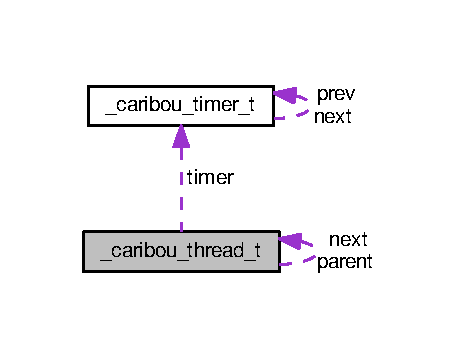
\includegraphics[width=220pt]{struct__caribou__thread__t__coll__graph}
\end{center}
\end{figure}
\subsection*{Data Fields}
\begin{DoxyCompactItemize}
\item 
struct \hyperlink{struct__caribou__thread__t}{\-\_\-caribou\-\_\-thread\-\_\-t} $\ast$ \hyperlink{struct__caribou__thread__t_a584ef536a58df0aa0e097add451a66e4}{next}
\begin{DoxyCompactList}\small\item\em Pointer to the next thread in the linked list. \end{DoxyCompactList}\item 
struct \hyperlink{struct__caribou__thread__t}{\-\_\-caribou\-\_\-thread\-\_\-t} $\ast$ \hyperlink{struct__caribou__thread__t_a1ecb216e2a946081e642ad98bbbbd9e7}{parent}
\begin{DoxyCompactList}\small\item\em Pointer to the parent thread of this thread. \end{DoxyCompactList}\item 
void $\ast$ \hyperlink{struct__caribou__thread__t_aceaf2820170f1252157576769bf04672}{sp}
\begin{DoxyCompactList}\small\item\em The stack pointer of this thread at the last entry point to the scheduler. \end{DoxyCompactList}\item 
void $\ast$ \hyperlink{struct__caribou__thread__t_af4ac7e484b60887e54aeff966cf366da}{stack\-\_\-usage}
\begin{DoxyCompactList}\small\item\em The \char`\"{}high-\/water\char`\"{} mark indicating the most stack used by the thread. \end{DoxyCompactList}\item 
void $\ast$ \hyperlink{struct__caribou__thread__t_a09703c14662151cf8b073626e9144279}{stack\-\_\-low}
\begin{DoxyCompactList}\small\item\em The \char`\"{}low-\/water\char`\"{} point at which free stack level is dangerously low. \end{DoxyCompactList}\item 
void $\ast$ \hyperlink{struct__caribou__thread__t_a82a114a6b3fb2c733159562ba9442eca}{stack\-\_\-top}
\begin{DoxyCompactList}\small\item\em Pointer to the top word of the thread's stack. \end{DoxyCompactList}\item 
void $\ast$ \hyperlink{struct__caribou__thread__t_a6e316e784c771be57958edcd9e95b8d9}{stack\-\_\-base}
\begin{DoxyCompactList}\small\item\em Pointer to the bottom of the thread's stack. \end{DoxyCompactList}\item 
uint16\-\_\-t \hyperlink{struct__caribou__thread__t_a9896ce34d6cb9832eca2456d281b2eec}{state}
\begin{DoxyCompactList}\small\item\em Flags to indicate the current state of the thread. \end{DoxyCompactList}\item 
int16\-\_\-t \hyperlink{struct__caribou__thread__t_a91f8936a0a3a5c21c4ffcbe1045c34ee}{prio}
\begin{DoxyCompactList}\small\item\em Thread priority -\/ currently implemented as a number of jiffies of run time -\/ higher number = more jiffies. \end{DoxyCompactList}\item 
const char $\ast$ \hyperlink{struct__caribou__thread__t_af6982a95fce8e2c99023a803d903707b}{name}
\begin{DoxyCompactList}\small\item\em A Pointer to the '\textbackslash{}0' terminated A\-S\-C\-I\-I name of the tread or N\-U\-L\-L. \end{DoxyCompactList}\item 
void $\ast$ \hyperlink{struct__caribou__thread__t_a35f2bbe0ed40746c1505382dbb5cd865}{arg}
\begin{DoxyCompactList}\small\item\em An optional argument pointer passed during the creation of the thread. \end{DoxyCompactList}\item 
uint64\-\_\-t \hyperlink{struct__caribou__thread__t_a942c87c4803e79dabc7fd0b5e24afb63}{runtime}
\begin{DoxyCompactList}\small\item\em The total run time of the thread expressed in jiffies. \end{DoxyCompactList}\item 
int16\-\_\-t \hyperlink{struct__caribou__thread__t_a3f291721c2674ea6c5776d014357144b}{lock}
\begin{DoxyCompactList}\small\item\em Thread lock count incremented on \hyperlink{thread_8h_a81ec8b7e5f2accca0c462337830fbdf5}{caribou\-\_\-thread\-\_\-lock()}, decremented on \hyperlink{thread_8h_a0b4d0cd341028e7713f6f0f60a018529}{caribou\-\_\-thread\-\_\-unlock()} \end{DoxyCompactList}\item 
void($\ast$ \hyperlink{struct__caribou__thread__t_abf99478d61f893fa11b938c562a9ef20}{finishfn} )(void $\ast$)
\begin{DoxyCompactList}\small\item\em Callback function pointer which is called just pror to the thread being terminated, can be N\-U\-L\-L. \end{DoxyCompactList}\item 
\hyperlink{timer_8h_a83310ffb8b0e689ad504298d2b80ead7}{caribou\-\_\-timer\-\_\-t} $\ast$ \hyperlink{struct__caribou__thread__t_a0b044d7f5d93f8d457ff985f0f7e4bd3}{timer}
\begin{DoxyCompactList}\small\item\em A linked list of timers belong to this thread. \end{DoxyCompactList}\item 
\hyperlink{errno_8h_a46a037236862ac1a534efbe605c10f42}{errno\-\_\-t} \hyperlink{struct__caribou__thread__t_a4a14ec3ec88fb5528f43e53686271828}{errno}
\begin{DoxyCompactList}\small\item\em A copy of the global errno variable, preserved here on each context switch. \end{DoxyCompactList}\item 
int16\-\_\-t \hyperlink{struct__caribou__thread__t_a4a4746a8fede65c362fb46c80469509f}{sleep}
\begin{DoxyCompactList}\small\item\em The current sleep state ($<$=0\-: wakeup), ($>$0\-: sleep state). \end{DoxyCompactList}\end{DoxyCompactItemize}


\subsection{Detailed Description}
The definition of a thread structure. An instance of such a structure exists for each currently running thread. 

Definition at line 31 of file thread.\-h.



\subsection{Field Documentation}
\hypertarget{struct__caribou__thread__t_a35f2bbe0ed40746c1505382dbb5cd865}{\index{\-\_\-caribou\-\_\-thread\-\_\-t@{\-\_\-caribou\-\_\-thread\-\_\-t}!arg@{arg}}
\index{arg@{arg}!_caribou_thread_t@{\-\_\-caribou\-\_\-thread\-\_\-t}}
\subsubsection[{arg}]{\setlength{\rightskip}{0pt plus 5cm}void$\ast$ \-\_\-caribou\-\_\-thread\-\_\-t\-::arg}}\label{struct__caribou__thread__t_a35f2bbe0ed40746c1505382dbb5cd865}


An optional argument pointer passed during the creation of the thread. 



Definition at line 64 of file thread.\-h.

\hypertarget{struct__caribou__thread__t_a4a14ec3ec88fb5528f43e53686271828}{\index{\-\_\-caribou\-\_\-thread\-\_\-t@{\-\_\-caribou\-\_\-thread\-\_\-t}!errno@{errno}}
\index{errno@{errno}!_caribou_thread_t@{\-\_\-caribou\-\_\-thread\-\_\-t}}
\subsubsection[{errno}]{\setlength{\rightskip}{0pt plus 5cm}{\bf errno\-\_\-t} \-\_\-caribou\-\_\-thread\-\_\-t\-::errno}}\label{struct__caribou__thread__t_a4a14ec3ec88fb5528f43e53686271828}


A copy of the global errno variable, preserved here on each context switch. 



Definition at line 79 of file thread.\-h.

\hypertarget{struct__caribou__thread__t_abf99478d61f893fa11b938c562a9ef20}{\index{\-\_\-caribou\-\_\-thread\-\_\-t@{\-\_\-caribou\-\_\-thread\-\_\-t}!finishfn@{finishfn}}
\index{finishfn@{finishfn}!_caribou_thread_t@{\-\_\-caribou\-\_\-thread\-\_\-t}}
\subsubsection[{finishfn}]{\setlength{\rightskip}{0pt plus 5cm}void($\ast$ \-\_\-caribou\-\_\-thread\-\_\-t\-::finishfn)(void $\ast$)}}\label{struct__caribou__thread__t_abf99478d61f893fa11b938c562a9ef20}


Callback function pointer which is called just pror to the thread being terminated, can be N\-U\-L\-L. 



Definition at line 73 of file thread.\-h.

\hypertarget{struct__caribou__thread__t_a3f291721c2674ea6c5776d014357144b}{\index{\-\_\-caribou\-\_\-thread\-\_\-t@{\-\_\-caribou\-\_\-thread\-\_\-t}!lock@{lock}}
\index{lock@{lock}!_caribou_thread_t@{\-\_\-caribou\-\_\-thread\-\_\-t}}
\subsubsection[{lock}]{\setlength{\rightskip}{0pt plus 5cm}int16\-\_\-t \-\_\-caribou\-\_\-thread\-\_\-t\-::lock}}\label{struct__caribou__thread__t_a3f291721c2674ea6c5776d014357144b}


Thread lock count incremented on \hyperlink{thread_8h_a81ec8b7e5f2accca0c462337830fbdf5}{caribou\-\_\-thread\-\_\-lock()}, decremented on \hyperlink{thread_8h_a0b4d0cd341028e7713f6f0f60a018529}{caribou\-\_\-thread\-\_\-unlock()} 



Definition at line 70 of file thread.\-h.

\hypertarget{struct__caribou__thread__t_af6982a95fce8e2c99023a803d903707b}{\index{\-\_\-caribou\-\_\-thread\-\_\-t@{\-\_\-caribou\-\_\-thread\-\_\-t}!name@{name}}
\index{name@{name}!_caribou_thread_t@{\-\_\-caribou\-\_\-thread\-\_\-t}}
\subsubsection[{name}]{\setlength{\rightskip}{0pt plus 5cm}const char$\ast$ \-\_\-caribou\-\_\-thread\-\_\-t\-::name}}\label{struct__caribou__thread__t_af6982a95fce8e2c99023a803d903707b}


A Pointer to the '\textbackslash{}0' terminated A\-S\-C\-I\-I name of the tread or N\-U\-L\-L. 



Definition at line 61 of file thread.\-h.

\hypertarget{struct__caribou__thread__t_a584ef536a58df0aa0e097add451a66e4}{\index{\-\_\-caribou\-\_\-thread\-\_\-t@{\-\_\-caribou\-\_\-thread\-\_\-t}!next@{next}}
\index{next@{next}!_caribou_thread_t@{\-\_\-caribou\-\_\-thread\-\_\-t}}
\subsubsection[{next}]{\setlength{\rightskip}{0pt plus 5cm}struct {\bf \-\_\-caribou\-\_\-thread\-\_\-t}$\ast$ \-\_\-caribou\-\_\-thread\-\_\-t\-::next}}\label{struct__caribou__thread__t_a584ef536a58df0aa0e097add451a66e4}


Pointer to the next thread in the linked list. 



Definition at line 34 of file thread.\-h.

\hypertarget{struct__caribou__thread__t_a1ecb216e2a946081e642ad98bbbbd9e7}{\index{\-\_\-caribou\-\_\-thread\-\_\-t@{\-\_\-caribou\-\_\-thread\-\_\-t}!parent@{parent}}
\index{parent@{parent}!_caribou_thread_t@{\-\_\-caribou\-\_\-thread\-\_\-t}}
\subsubsection[{parent}]{\setlength{\rightskip}{0pt plus 5cm}struct {\bf \-\_\-caribou\-\_\-thread\-\_\-t}$\ast$ \-\_\-caribou\-\_\-thread\-\_\-t\-::parent}}\label{struct__caribou__thread__t_a1ecb216e2a946081e642ad98bbbbd9e7}


Pointer to the parent thread of this thread. 



Definition at line 37 of file thread.\-h.

\hypertarget{struct__caribou__thread__t_a91f8936a0a3a5c21c4ffcbe1045c34ee}{\index{\-\_\-caribou\-\_\-thread\-\_\-t@{\-\_\-caribou\-\_\-thread\-\_\-t}!prio@{prio}}
\index{prio@{prio}!_caribou_thread_t@{\-\_\-caribou\-\_\-thread\-\_\-t}}
\subsubsection[{prio}]{\setlength{\rightskip}{0pt plus 5cm}int16\-\_\-t \-\_\-caribou\-\_\-thread\-\_\-t\-::prio}}\label{struct__caribou__thread__t_a91f8936a0a3a5c21c4ffcbe1045c34ee}


Thread priority -\/ currently implemented as a number of jiffies of run time -\/ higher number = more jiffies. 



Definition at line 58 of file thread.\-h.

\hypertarget{struct__caribou__thread__t_a942c87c4803e79dabc7fd0b5e24afb63}{\index{\-\_\-caribou\-\_\-thread\-\_\-t@{\-\_\-caribou\-\_\-thread\-\_\-t}!runtime@{runtime}}
\index{runtime@{runtime}!_caribou_thread_t@{\-\_\-caribou\-\_\-thread\-\_\-t}}
\subsubsection[{runtime}]{\setlength{\rightskip}{0pt plus 5cm}uint64\-\_\-t \-\_\-caribou\-\_\-thread\-\_\-t\-::runtime}}\label{struct__caribou__thread__t_a942c87c4803e79dabc7fd0b5e24afb63}


The total run time of the thread expressed in jiffies. 



Definition at line 67 of file thread.\-h.

\hypertarget{struct__caribou__thread__t_a4a4746a8fede65c362fb46c80469509f}{\index{\-\_\-caribou\-\_\-thread\-\_\-t@{\-\_\-caribou\-\_\-thread\-\_\-t}!sleep@{sleep}}
\index{sleep@{sleep}!_caribou_thread_t@{\-\_\-caribou\-\_\-thread\-\_\-t}}
\subsubsection[{sleep}]{\setlength{\rightskip}{0pt plus 5cm}int16\-\_\-t \-\_\-caribou\-\_\-thread\-\_\-t\-::sleep}}\label{struct__caribou__thread__t_a4a4746a8fede65c362fb46c80469509f}


The current sleep state ($<$=0\-: wakeup), ($>$0\-: sleep state). 

\begin{DoxyNote}{Note}
The main thread can never sleep. 
\end{DoxyNote}


Definition at line 82 of file thread.\-h.

\hypertarget{struct__caribou__thread__t_aceaf2820170f1252157576769bf04672}{\index{\-\_\-caribou\-\_\-thread\-\_\-t@{\-\_\-caribou\-\_\-thread\-\_\-t}!sp@{sp}}
\index{sp@{sp}!_caribou_thread_t@{\-\_\-caribou\-\_\-thread\-\_\-t}}
\subsubsection[{sp}]{\setlength{\rightskip}{0pt plus 5cm}void$\ast$ \-\_\-caribou\-\_\-thread\-\_\-t\-::sp}}\label{struct__caribou__thread__t_aceaf2820170f1252157576769bf04672}


The stack pointer of this thread at the last entry point to the scheduler. 



Definition at line 40 of file thread.\-h.

\hypertarget{struct__caribou__thread__t_a6e316e784c771be57958edcd9e95b8d9}{\index{\-\_\-caribou\-\_\-thread\-\_\-t@{\-\_\-caribou\-\_\-thread\-\_\-t}!stack\-\_\-base@{stack\-\_\-base}}
\index{stack\-\_\-base@{stack\-\_\-base}!_caribou_thread_t@{\-\_\-caribou\-\_\-thread\-\_\-t}}
\subsubsection[{stack\-\_\-base}]{\setlength{\rightskip}{0pt plus 5cm}void$\ast$ \-\_\-caribou\-\_\-thread\-\_\-t\-::stack\-\_\-base}}\label{struct__caribou__thread__t_a6e316e784c771be57958edcd9e95b8d9}


Pointer to the bottom of the thread's stack. 



Definition at line 52 of file thread.\-h.

\hypertarget{struct__caribou__thread__t_a09703c14662151cf8b073626e9144279}{\index{\-\_\-caribou\-\_\-thread\-\_\-t@{\-\_\-caribou\-\_\-thread\-\_\-t}!stack\-\_\-low@{stack\-\_\-low}}
\index{stack\-\_\-low@{stack\-\_\-low}!_caribou_thread_t@{\-\_\-caribou\-\_\-thread\-\_\-t}}
\subsubsection[{stack\-\_\-low}]{\setlength{\rightskip}{0pt plus 5cm}void$\ast$ \-\_\-caribou\-\_\-thread\-\_\-t\-::stack\-\_\-low}}\label{struct__caribou__thread__t_a09703c14662151cf8b073626e9144279}


The \char`\"{}low-\/water\char`\"{} point at which free stack level is dangerously low. 



Definition at line 46 of file thread.\-h.

\hypertarget{struct__caribou__thread__t_a82a114a6b3fb2c733159562ba9442eca}{\index{\-\_\-caribou\-\_\-thread\-\_\-t@{\-\_\-caribou\-\_\-thread\-\_\-t}!stack\-\_\-top@{stack\-\_\-top}}
\index{stack\-\_\-top@{stack\-\_\-top}!_caribou_thread_t@{\-\_\-caribou\-\_\-thread\-\_\-t}}
\subsubsection[{stack\-\_\-top}]{\setlength{\rightskip}{0pt plus 5cm}void$\ast$ \-\_\-caribou\-\_\-thread\-\_\-t\-::stack\-\_\-top}}\label{struct__caribou__thread__t_a82a114a6b3fb2c733159562ba9442eca}


Pointer to the top word of the thread's stack. 



Definition at line 49 of file thread.\-h.

\hypertarget{struct__caribou__thread__t_af4ac7e484b60887e54aeff966cf366da}{\index{\-\_\-caribou\-\_\-thread\-\_\-t@{\-\_\-caribou\-\_\-thread\-\_\-t}!stack\-\_\-usage@{stack\-\_\-usage}}
\index{stack\-\_\-usage@{stack\-\_\-usage}!_caribou_thread_t@{\-\_\-caribou\-\_\-thread\-\_\-t}}
\subsubsection[{stack\-\_\-usage}]{\setlength{\rightskip}{0pt plus 5cm}void$\ast$ \-\_\-caribou\-\_\-thread\-\_\-t\-::stack\-\_\-usage}}\label{struct__caribou__thread__t_af4ac7e484b60887e54aeff966cf366da}


The \char`\"{}high-\/water\char`\"{} mark indicating the most stack used by the thread. 



Definition at line 43 of file thread.\-h.

\hypertarget{struct__caribou__thread__t_a9896ce34d6cb9832eca2456d281b2eec}{\index{\-\_\-caribou\-\_\-thread\-\_\-t@{\-\_\-caribou\-\_\-thread\-\_\-t}!state@{state}}
\index{state@{state}!_caribou_thread_t@{\-\_\-caribou\-\_\-thread\-\_\-t}}
\subsubsection[{state}]{\setlength{\rightskip}{0pt plus 5cm}uint16\-\_\-t \-\_\-caribou\-\_\-thread\-\_\-t\-::state}}\label{struct__caribou__thread__t_a9896ce34d6cb9832eca2456d281b2eec}


Flags to indicate the current state of the thread. 



Definition at line 55 of file thread.\-h.

\hypertarget{struct__caribou__thread__t_a0b044d7f5d93f8d457ff985f0f7e4bd3}{\index{\-\_\-caribou\-\_\-thread\-\_\-t@{\-\_\-caribou\-\_\-thread\-\_\-t}!timer@{timer}}
\index{timer@{timer}!_caribou_thread_t@{\-\_\-caribou\-\_\-thread\-\_\-t}}
\subsubsection[{timer}]{\setlength{\rightskip}{0pt plus 5cm}{\bf caribou\-\_\-timer\-\_\-t}$\ast$ \-\_\-caribou\-\_\-thread\-\_\-t\-::timer}}\label{struct__caribou__thread__t_a0b044d7f5d93f8d457ff985f0f7e4bd3}


A linked list of timers belong to this thread. 



Definition at line 76 of file thread.\-h.



The documentation for this struct was generated from the following file\-:\begin{DoxyCompactItemize}
\item 
include/caribou/kernel/\hyperlink{thread_8h}{thread.\-h}\end{DoxyCompactItemize}

\hypertarget{struct__caribou__timer__t}{\section{\-\_\-caribou\-\_\-timer\-\_\-t Struct Reference}
\label{struct__caribou__timer__t}\index{\-\_\-caribou\-\_\-timer\-\_\-t@{\-\_\-caribou\-\_\-timer\-\_\-t}}
}


The caribou\-\_\-timer\-\_\-t structure defines the data structure used by C\-A\-R\-I\-B\-O\-U to maintain timers and sleep periods.  




{\ttfamily \#include $<$timer.\-h$>$}



Collaboration diagram for \-\_\-caribou\-\_\-timer\-\_\-t\-:\nopagebreak
\begin{figure}[H]
\begin{center}
\leavevmode
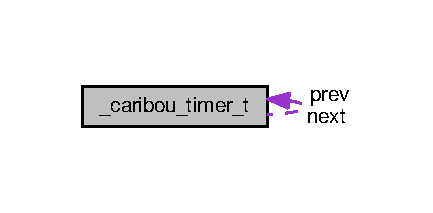
\includegraphics[width=208pt]{struct__caribou__timer__t__coll__graph}
\end{center}
\end{figure}
\subsection*{Data Fields}
\begin{DoxyCompactItemize}
\item 
struct \hyperlink{struct__caribou__timer__t}{\-\_\-caribou\-\_\-timer\-\_\-t} $\ast$ \hyperlink{struct__caribou__timer__t_a711f3f84b0ef799261b12d7c0a6d4132}{prev}
\begin{DoxyCompactList}\small\item\em A pointer to the previous caribou\-\_\-timer\-\_\-t in the linked list. \end{DoxyCompactList}\item 
struct \hyperlink{struct__caribou__timer__t}{\-\_\-caribou\-\_\-timer\-\_\-t} $\ast$ \hyperlink{struct__caribou__timer__t_a922fab9a09a701c3ac7273c9548a4afa}{next}
\begin{DoxyCompactList}\small\item\em A pointer to the next caribou\-\_\-timer\-\_\-t in the linked list. \end{DoxyCompactList}\item 
\hyperlink{timer_8h_af991f5bbba685d64fd4a78090140228b}{caribou\-\_\-timer\-\_\-callback\-\_\-fn} $\ast$ \hyperlink{struct__caribou__timer__t_a036d01df45a585775dd0ef585f90eb7a}{timerfn}
\begin{DoxyCompactList}\small\item\em Optional timer notification callback function. \end{DoxyCompactList}\item 
void $\ast$ \hyperlink{struct__caribou__timer__t_a9276b37ed4a76264b1f8570b678abe42}{fnarg}
\begin{DoxyCompactList}\small\item\em Optional timer notification callback function argument. \end{DoxyCompactList}\item 
uint32\-\_\-t \hyperlink{struct__caribou__timer__t_a94c03a7c23a27aa378b861389b6ee0c8}{ticks}
\begin{DoxyCompactList}\small\item\em The remaining ticks (iffies) before the timer is due to expire. \end{DoxyCompactList}\item 
uint32\-\_\-t \hyperlink{struct__caribou__timer__t_a1b66f8c7abf7e00efa3d0adc916b0ecd}{reloadticks}
\begin{DoxyCompactList}\small\item\em The tick count to re-\/load in order to re-\/start the timer period. \end{DoxyCompactList}\item 
uint8\-\_\-t \hyperlink{struct__caribou__timer__t_a492a012c1141298c40a781c09ca86aed}{flags}
\begin{DoxyCompactList}\small\item\em The lags which control various timer operations. \end{DoxyCompactList}\end{DoxyCompactItemize}


\subsection{Detailed Description}
The caribou\-\_\-timer\-\_\-t structure defines the data structure used by C\-A\-R\-I\-B\-O\-U to maintain timers and sleep periods. 

\begin{DoxyNote}{Note}
The structure elements should not be manipulated by the application program, and are subject to change in future releases. 
\end{DoxyNote}


Definition at line 56 of file timer.\-h.



\subsection{Field Documentation}
\hypertarget{struct__caribou__timer__t_a492a012c1141298c40a781c09ca86aed}{\index{\-\_\-caribou\-\_\-timer\-\_\-t@{\-\_\-caribou\-\_\-timer\-\_\-t}!flags@{flags}}
\index{flags@{flags}!_caribou_timer_t@{\-\_\-caribou\-\_\-timer\-\_\-t}}
\subsubsection[{flags}]{\setlength{\rightskip}{0pt plus 5cm}uint8\-\_\-t \-\_\-caribou\-\_\-timer\-\_\-t\-::flags}}\label{struct__caribou__timer__t_a492a012c1141298c40a781c09ca86aed}


The lags which control various timer operations. 



Definition at line 71 of file timer.\-h.

\hypertarget{struct__caribou__timer__t_a9276b37ed4a76264b1f8570b678abe42}{\index{\-\_\-caribou\-\_\-timer\-\_\-t@{\-\_\-caribou\-\_\-timer\-\_\-t}!fnarg@{fnarg}}
\index{fnarg@{fnarg}!_caribou_timer_t@{\-\_\-caribou\-\_\-timer\-\_\-t}}
\subsubsection[{fnarg}]{\setlength{\rightskip}{0pt plus 5cm}void$\ast$ \-\_\-caribou\-\_\-timer\-\_\-t\-::fnarg}}\label{struct__caribou__timer__t_a9276b37ed4a76264b1f8570b678abe42}


Optional timer notification callback function argument. 



Definition at line 65 of file timer.\-h.

\hypertarget{struct__caribou__timer__t_a922fab9a09a701c3ac7273c9548a4afa}{\index{\-\_\-caribou\-\_\-timer\-\_\-t@{\-\_\-caribou\-\_\-timer\-\_\-t}!next@{next}}
\index{next@{next}!_caribou_timer_t@{\-\_\-caribou\-\_\-timer\-\_\-t}}
\subsubsection[{next}]{\setlength{\rightskip}{0pt plus 5cm}struct {\bf \-\_\-caribou\-\_\-timer\-\_\-t}$\ast$ \-\_\-caribou\-\_\-timer\-\_\-t\-::next}}\label{struct__caribou__timer__t_a922fab9a09a701c3ac7273c9548a4afa}


A pointer to the next caribou\-\_\-timer\-\_\-t in the linked list. 



Definition at line 61 of file timer.\-h.

\hypertarget{struct__caribou__timer__t_a711f3f84b0ef799261b12d7c0a6d4132}{\index{\-\_\-caribou\-\_\-timer\-\_\-t@{\-\_\-caribou\-\_\-timer\-\_\-t}!prev@{prev}}
\index{prev@{prev}!_caribou_timer_t@{\-\_\-caribou\-\_\-timer\-\_\-t}}
\subsubsection[{prev}]{\setlength{\rightskip}{0pt plus 5cm}struct {\bf \-\_\-caribou\-\_\-timer\-\_\-t}$\ast$ \-\_\-caribou\-\_\-timer\-\_\-t\-::prev}}\label{struct__caribou__timer__t_a711f3f84b0ef799261b12d7c0a6d4132}


A pointer to the previous caribou\-\_\-timer\-\_\-t in the linked list. 



Definition at line 59 of file timer.\-h.

\hypertarget{struct__caribou__timer__t_a1b66f8c7abf7e00efa3d0adc916b0ecd}{\index{\-\_\-caribou\-\_\-timer\-\_\-t@{\-\_\-caribou\-\_\-timer\-\_\-t}!reloadticks@{reloadticks}}
\index{reloadticks@{reloadticks}!_caribou_timer_t@{\-\_\-caribou\-\_\-timer\-\_\-t}}
\subsubsection[{reloadticks}]{\setlength{\rightskip}{0pt plus 5cm}uint32\-\_\-t \-\_\-caribou\-\_\-timer\-\_\-t\-::reloadticks}}\label{struct__caribou__timer__t_a1b66f8c7abf7e00efa3d0adc916b0ecd}


The tick count to re-\/load in order to re-\/start the timer period. 



Definition at line 69 of file timer.\-h.

\hypertarget{struct__caribou__timer__t_a94c03a7c23a27aa378b861389b6ee0c8}{\index{\-\_\-caribou\-\_\-timer\-\_\-t@{\-\_\-caribou\-\_\-timer\-\_\-t}!ticks@{ticks}}
\index{ticks@{ticks}!_caribou_timer_t@{\-\_\-caribou\-\_\-timer\-\_\-t}}
\subsubsection[{ticks}]{\setlength{\rightskip}{0pt plus 5cm}uint32\-\_\-t \-\_\-caribou\-\_\-timer\-\_\-t\-::ticks}}\label{struct__caribou__timer__t_a94c03a7c23a27aa378b861389b6ee0c8}


The remaining ticks (iffies) before the timer is due to expire. 



Definition at line 67 of file timer.\-h.

\hypertarget{struct__caribou__timer__t_a036d01df45a585775dd0ef585f90eb7a}{\index{\-\_\-caribou\-\_\-timer\-\_\-t@{\-\_\-caribou\-\_\-timer\-\_\-t}!timerfn@{timerfn}}
\index{timerfn@{timerfn}!_caribou_timer_t@{\-\_\-caribou\-\_\-timer\-\_\-t}}
\subsubsection[{timerfn}]{\setlength{\rightskip}{0pt plus 5cm}{\bf caribou\-\_\-timer\-\_\-callback\-\_\-fn}$\ast$ \-\_\-caribou\-\_\-timer\-\_\-t\-::timerfn}}\label{struct__caribou__timer__t_a036d01df45a585775dd0ef585f90eb7a}


Optional timer notification callback function. 



Definition at line 63 of file timer.\-h.



The documentation for this struct was generated from the following file\-:\begin{DoxyCompactItemize}
\item 
include/caribou/kernel/\hyperlink{timer_8h}{timer.\-h}\end{DoxyCompactItemize}

\hypertarget{struct__stdio__t}{\section{\-\_\-stdio\-\_\-t Struct Reference}
\label{struct__stdio__t}\index{\-\_\-stdio\-\_\-t@{\-\_\-stdio\-\_\-t}}
}


{\ttfamily \#include $<$stdio.\-h$>$}

\subsection*{Data Fields}
\begin{DoxyCompactItemize}
\item 
void $\ast$ \hyperlink{struct__stdio__t_abe889179e50490e5eb8d2a3592166638}{device\-\_\-private}
\item 
int($\ast$ \hyperlink{struct__stdio__t_a3698bb7d1020290bd662cf2e31c9d2c9}{readfn} )(struct \hyperlink{struct__stdio__t}{\-\_\-stdio\-\_\-t} $\ast$, void $\ast$, int)
\begin{DoxyCompactList}\small\item\em Device Driver private data. \end{DoxyCompactList}\item 
int($\ast$ \hyperlink{struct__stdio__t_aa50ed1df960be87cd28e05a1df7e9ddd}{writefn} )(struct \hyperlink{struct__stdio__t}{\-\_\-stdio\-\_\-t} $\ast$, void $\ast$, int)
\begin{DoxyCompactList}\small\item\em Device Driver read-\/data function. \end{DoxyCompactList}\item 
int($\ast$ \hyperlink{struct__stdio__t_a302b5c7d886e2ad5831e7fb40129d10e}{readqueuefn} )(struct \hyperlink{struct__stdio__t}{\-\_\-stdio\-\_\-t} $\ast$)
\begin{DoxyCompactList}\small\item\em Device Driver write-\/data function. \end{DoxyCompactList}\item 
int($\ast$ \hyperlink{struct__stdio__t_ae78e9d8689c33c835ac7551504937851}{writequeuefn} )(struct \hyperlink{struct__stdio__t}{\-\_\-stdio\-\_\-t} $\ast$)
\begin{DoxyCompactList}\small\item\em Device Driver read-\/data available function. \end{DoxyCompactList}\item 
int($\ast$ \hyperlink{struct__stdio__t_ac2642f9c5da1a64df85c6d67783a75e2}{statefn} )(struct \hyperlink{struct__stdio__t}{\-\_\-stdio\-\_\-t} $\ast$)
\begin{DoxyCompactList}\small\item\em Device Driver write-\/data pending. \end{DoxyCompactList}\end{DoxyCompactItemize}


\subsection{Detailed Description}


Definition at line 32 of file stdio.\-h.



\subsection{Field Documentation}
\hypertarget{struct__stdio__t_abe889179e50490e5eb8d2a3592166638}{\index{\-\_\-stdio\-\_\-t@{\-\_\-stdio\-\_\-t}!device\-\_\-private@{device\-\_\-private}}
\index{device\-\_\-private@{device\-\_\-private}!_stdio_t@{\-\_\-stdio\-\_\-t}}
\subsubsection[{device\-\_\-private}]{\setlength{\rightskip}{0pt plus 5cm}void$\ast$ \-\_\-stdio\-\_\-t\-::device\-\_\-private}}\label{struct__stdio__t_abe889179e50490e5eb8d2a3592166638}


Definition at line 34 of file stdio.\-h.

\hypertarget{struct__stdio__t_a3698bb7d1020290bd662cf2e31c9d2c9}{\index{\-\_\-stdio\-\_\-t@{\-\_\-stdio\-\_\-t}!readfn@{readfn}}
\index{readfn@{readfn}!_stdio_t@{\-\_\-stdio\-\_\-t}}
\subsubsection[{readfn}]{\setlength{\rightskip}{0pt plus 5cm}int($\ast$ \-\_\-stdio\-\_\-t\-::readfn)(struct {\bf \-\_\-stdio\-\_\-t} $\ast$, void $\ast$, int)}}\label{struct__stdio__t_a3698bb7d1020290bd662cf2e31c9d2c9}


Device Driver private data. 



Definition at line 35 of file stdio.\-h.

\hypertarget{struct__stdio__t_a302b5c7d886e2ad5831e7fb40129d10e}{\index{\-\_\-stdio\-\_\-t@{\-\_\-stdio\-\_\-t}!readqueuefn@{readqueuefn}}
\index{readqueuefn@{readqueuefn}!_stdio_t@{\-\_\-stdio\-\_\-t}}
\subsubsection[{readqueuefn}]{\setlength{\rightskip}{0pt plus 5cm}int($\ast$ \-\_\-stdio\-\_\-t\-::readqueuefn)(struct {\bf \-\_\-stdio\-\_\-t} $\ast$)}}\label{struct__stdio__t_a302b5c7d886e2ad5831e7fb40129d10e}


Device Driver write-\/data function. 



Definition at line 37 of file stdio.\-h.

\hypertarget{struct__stdio__t_ac2642f9c5da1a64df85c6d67783a75e2}{\index{\-\_\-stdio\-\_\-t@{\-\_\-stdio\-\_\-t}!statefn@{statefn}}
\index{statefn@{statefn}!_stdio_t@{\-\_\-stdio\-\_\-t}}
\subsubsection[{statefn}]{\setlength{\rightskip}{0pt plus 5cm}int($\ast$ \-\_\-stdio\-\_\-t\-::statefn)(struct {\bf \-\_\-stdio\-\_\-t} $\ast$)}}\label{struct__stdio__t_ac2642f9c5da1a64df85c6d67783a75e2}


Device Driver write-\/data pending. 



Definition at line 39 of file stdio.\-h.

\hypertarget{struct__stdio__t_aa50ed1df960be87cd28e05a1df7e9ddd}{\index{\-\_\-stdio\-\_\-t@{\-\_\-stdio\-\_\-t}!writefn@{writefn}}
\index{writefn@{writefn}!_stdio_t@{\-\_\-stdio\-\_\-t}}
\subsubsection[{writefn}]{\setlength{\rightskip}{0pt plus 5cm}int($\ast$ \-\_\-stdio\-\_\-t\-::writefn)(struct {\bf \-\_\-stdio\-\_\-t} $\ast$, void $\ast$, int)}}\label{struct__stdio__t_aa50ed1df960be87cd28e05a1df7e9ddd}


Device Driver read-\/data function. 



Definition at line 36 of file stdio.\-h.

\hypertarget{struct__stdio__t_ae78e9d8689c33c835ac7551504937851}{\index{\-\_\-stdio\-\_\-t@{\-\_\-stdio\-\_\-t}!writequeuefn@{writequeuefn}}
\index{writequeuefn@{writequeuefn}!_stdio_t@{\-\_\-stdio\-\_\-t}}
\subsubsection[{writequeuefn}]{\setlength{\rightskip}{0pt plus 5cm}int($\ast$ \-\_\-stdio\-\_\-t\-::writequeuefn)(struct {\bf \-\_\-stdio\-\_\-t} $\ast$)}}\label{struct__stdio__t_ae78e9d8689c33c835ac7551504937851}


Device Driver read-\/data available function. 



Definition at line 38 of file stdio.\-h.



The documentation for this struct was generated from the following file\-:\begin{DoxyCompactItemize}
\item 
include/caribou/lib/\hyperlink{stdio_8h}{stdio.\-h}\end{DoxyCompactItemize}

\hypertarget{structcaribou__adc__t}{\section{caribou\-\_\-adc\-\_\-t Struct Reference}
\label{structcaribou__adc__t}\index{caribou\-\_\-adc\-\_\-t@{caribou\-\_\-adc\-\_\-t}}
}


{\ttfamily \#include $<$adc.\-h$>$}

\subsection*{Data Fields}
\begin{DoxyCompactItemize}
\item 
chip\-\_\-adc\-\_\-port\-\_\-t \hyperlink{structcaribou__adc__t_a81d68d4d24e7fd693a001d92a96a2e52}{port}
\item 
chip\-\_\-adc\-\_\-channel\-\_\-t \hyperlink{structcaribou__adc__t_ad7e1d6b340173ec1b982221bfd888a4c}{channel}
\end{DoxyCompactItemize}


\subsection{Detailed Description}


Definition at line 32 of file adc.\-h.



\subsection{Field Documentation}
\hypertarget{structcaribou__adc__t_ad7e1d6b340173ec1b982221bfd888a4c}{\index{caribou\-\_\-adc\-\_\-t@{caribou\-\_\-adc\-\_\-t}!channel@{channel}}
\index{channel@{channel}!caribou_adc_t@{caribou\-\_\-adc\-\_\-t}}
\subsubsection[{channel}]{\setlength{\rightskip}{0pt plus 5cm}chip\-\_\-adc\-\_\-channel\-\_\-t caribou\-\_\-adc\-\_\-t\-::channel}}\label{structcaribou__adc__t_ad7e1d6b340173ec1b982221bfd888a4c}


Definition at line 35 of file adc.\-h.

\hypertarget{structcaribou__adc__t_a81d68d4d24e7fd693a001d92a96a2e52}{\index{caribou\-\_\-adc\-\_\-t@{caribou\-\_\-adc\-\_\-t}!port@{port}}
\index{port@{port}!caribou_adc_t@{caribou\-\_\-adc\-\_\-t}}
\subsubsection[{port}]{\setlength{\rightskip}{0pt plus 5cm}chip\-\_\-adc\-\_\-port\-\_\-t caribou\-\_\-adc\-\_\-t\-::port}}\label{structcaribou__adc__t_a81d68d4d24e7fd693a001d92a96a2e52}


Definition at line 34 of file adc.\-h.



The documentation for this struct was generated from the following file\-:\begin{DoxyCompactItemize}
\item 
include/caribou/dev/\hyperlink{adc_8h}{adc.\-h}\end{DoxyCompactItemize}

\hypertarget{structcaribou__bytequeue__t}{\section{caribou\-\_\-bytequeue\-\_\-t Struct Reference}
\label{structcaribou__bytequeue__t}\index{caribou\-\_\-bytequeue\-\_\-t@{caribou\-\_\-bytequeue\-\_\-t}}
}


{\ttfamily \#include $<$bytequeue.\-h$>$}

\subsection*{Data Fields}
\begin{DoxyCompactItemize}
\item 
uint8\-\_\-t $\ast$ \hyperlink{structcaribou__bytequeue__t_a4a4aa3f8ed5e7e7e66f7da7a2cb7720e}{queue}
\item 
uint16\-\_\-t \hyperlink{structcaribou__bytequeue__t_a0f88b0ee081def2ac171173e3e520980}{size}
\begin{DoxyCompactList}\small\item\em The receive buffer. \end{DoxyCompactList}\item 
uint16\-\_\-t \hyperlink{structcaribou__bytequeue__t_a5dc9b7ce1ee37c0ca3dc5cb37650aa4b}{head}
\begin{DoxyCompactList}\small\item\em The receive buffer size. \end{DoxyCompactList}\item 
uint16\-\_\-t \hyperlink{structcaribou__bytequeue__t_a566eaeca029373cd7f187cc2e622b3f8}{tail}
\begin{DoxyCompactList}\small\item\em The receive buffer head pointer. \end{DoxyCompactList}\end{DoxyCompactItemize}


\subsection{Detailed Description}
Byte queues. 

Definition at line 29 of file bytequeue.\-h.



\subsection{Field Documentation}
\hypertarget{structcaribou__bytequeue__t_a5dc9b7ce1ee37c0ca3dc5cb37650aa4b}{\index{caribou\-\_\-bytequeue\-\_\-t@{caribou\-\_\-bytequeue\-\_\-t}!head@{head}}
\index{head@{head}!caribou_bytequeue_t@{caribou\-\_\-bytequeue\-\_\-t}}
\subsubsection[{head}]{\setlength{\rightskip}{0pt plus 5cm}uint16\-\_\-t caribou\-\_\-bytequeue\-\_\-t\-::head}}\label{structcaribou__bytequeue__t_a5dc9b7ce1ee37c0ca3dc5cb37650aa4b}


The receive buffer size. 



Definition at line 33 of file bytequeue.\-h.

\hypertarget{structcaribou__bytequeue__t_a4a4aa3f8ed5e7e7e66f7da7a2cb7720e}{\index{caribou\-\_\-bytequeue\-\_\-t@{caribou\-\_\-bytequeue\-\_\-t}!queue@{queue}}
\index{queue@{queue}!caribou_bytequeue_t@{caribou\-\_\-bytequeue\-\_\-t}}
\subsubsection[{queue}]{\setlength{\rightskip}{0pt plus 5cm}uint8\-\_\-t$\ast$ caribou\-\_\-bytequeue\-\_\-t\-::queue}}\label{structcaribou__bytequeue__t_a4a4aa3f8ed5e7e7e66f7da7a2cb7720e}


Definition at line 31 of file bytequeue.\-h.

\hypertarget{structcaribou__bytequeue__t_a0f88b0ee081def2ac171173e3e520980}{\index{caribou\-\_\-bytequeue\-\_\-t@{caribou\-\_\-bytequeue\-\_\-t}!size@{size}}
\index{size@{size}!caribou_bytequeue_t@{caribou\-\_\-bytequeue\-\_\-t}}
\subsubsection[{size}]{\setlength{\rightskip}{0pt plus 5cm}uint16\-\_\-t caribou\-\_\-bytequeue\-\_\-t\-::size}}\label{structcaribou__bytequeue__t_a0f88b0ee081def2ac171173e3e520980}


The receive buffer. 



Definition at line 32 of file bytequeue.\-h.

\hypertarget{structcaribou__bytequeue__t_a566eaeca029373cd7f187cc2e622b3f8}{\index{caribou\-\_\-bytequeue\-\_\-t@{caribou\-\_\-bytequeue\-\_\-t}!tail@{tail}}
\index{tail@{tail}!caribou_bytequeue_t@{caribou\-\_\-bytequeue\-\_\-t}}
\subsubsection[{tail}]{\setlength{\rightskip}{0pt plus 5cm}uint16\-\_\-t caribou\-\_\-bytequeue\-\_\-t\-::tail}}\label{structcaribou__bytequeue__t_a566eaeca029373cd7f187cc2e622b3f8}


The receive buffer head pointer. 



Definition at line 34 of file bytequeue.\-h.



The documentation for this struct was generated from the following file\-:\begin{DoxyCompactItemize}
\item 
include/caribou/lib/\hyperlink{bytequeue_8h}{bytequeue.\-h}\end{DoxyCompactItemize}

\hypertarget{structcaribou__gpio__t}{\section{caribou\-\_\-gpio\-\_\-t Struct Reference}
\label{structcaribou__gpio__t}\index{caribou\-\_\-gpio\-\_\-t@{caribou\-\_\-gpio\-\_\-t}}
}


{\ttfamily \#include $<$gpio.\-h$>$}

\subsection*{Data Fields}
\begin{DoxyCompactItemize}
\item 
chip\-\_\-gpio\-\_\-port\-\_\-t \hyperlink{structcaribou__gpio__t_ab474b09a256ab1cb97f704a5233f143b}{port}
\item 
chip\-\_\-gpio\-\_\-pinmask\-\_\-t \hyperlink{structcaribou__gpio__t_a176db98ba5783d4842ffd1b475d5bae2}{pinmask}
\end{DoxyCompactItemize}


\subsection{Detailed Description}


Definition at line 26 of file gpio.\-h.



\subsection{Field Documentation}
\hypertarget{structcaribou__gpio__t_a176db98ba5783d4842ffd1b475d5bae2}{\index{caribou\-\_\-gpio\-\_\-t@{caribou\-\_\-gpio\-\_\-t}!pinmask@{pinmask}}
\index{pinmask@{pinmask}!caribou_gpio_t@{caribou\-\_\-gpio\-\_\-t}}
\subsubsection[{pinmask}]{\setlength{\rightskip}{0pt plus 5cm}chip\-\_\-gpio\-\_\-pinmask\-\_\-t caribou\-\_\-gpio\-\_\-t\-::pinmask}}\label{structcaribou__gpio__t_a176db98ba5783d4842ffd1b475d5bae2}


Definition at line 29 of file gpio.\-h.

\hypertarget{structcaribou__gpio__t_ab474b09a256ab1cb97f704a5233f143b}{\index{caribou\-\_\-gpio\-\_\-t@{caribou\-\_\-gpio\-\_\-t}!port@{port}}
\index{port@{port}!caribou_gpio_t@{caribou\-\_\-gpio\-\_\-t}}
\subsubsection[{port}]{\setlength{\rightskip}{0pt plus 5cm}chip\-\_\-gpio\-\_\-port\-\_\-t caribou\-\_\-gpio\-\_\-t\-::port}}\label{structcaribou__gpio__t_ab474b09a256ab1cb97f704a5233f143b}


Definition at line 28 of file gpio.\-h.



The documentation for this struct was generated from the following file\-:\begin{DoxyCompactItemize}
\item 
include/caribou/dev/\hyperlink{gpio_8h}{gpio.\-h}\end{DoxyCompactItemize}

\hypertarget{structcaribou__i2c__t}{\section{caribou\-\_\-i2c\-\_\-t Struct Reference}
\label{structcaribou__i2c__t}\index{caribou\-\_\-i2c\-\_\-t@{caribou\-\_\-i2c\-\_\-t}}
}


{\ttfamily \#include $<$i2c.\-h$>$}

\subsection*{Data Fields}
\begin{DoxyCompactItemize}
\item 
chip\-\_\-i2c\-\_\-port\-\_\-t \hyperlink{structcaribou__i2c__t_af3ea37eae556cf758bc347d1dd6274b0}{port}
\item 
uint8\-\_\-t \hyperlink{structcaribou__i2c__t_a6231ff9a19bc1e0abef8f6d036ccef7f}{device\-\_\-address}
\end{DoxyCompactItemize}


\subsection{Detailed Description}


Definition at line 26 of file i2c.\-h.



\subsection{Field Documentation}
\hypertarget{structcaribou__i2c__t_a6231ff9a19bc1e0abef8f6d036ccef7f}{\index{caribou\-\_\-i2c\-\_\-t@{caribou\-\_\-i2c\-\_\-t}!device\-\_\-address@{device\-\_\-address}}
\index{device\-\_\-address@{device\-\_\-address}!caribou_i2c_t@{caribou\-\_\-i2c\-\_\-t}}
\subsubsection[{device\-\_\-address}]{\setlength{\rightskip}{0pt plus 5cm}uint8\-\_\-t caribou\-\_\-i2c\-\_\-t\-::device\-\_\-address}}\label{structcaribou__i2c__t_a6231ff9a19bc1e0abef8f6d036ccef7f}


Definition at line 29 of file i2c.\-h.

\hypertarget{structcaribou__i2c__t_af3ea37eae556cf758bc347d1dd6274b0}{\index{caribou\-\_\-i2c\-\_\-t@{caribou\-\_\-i2c\-\_\-t}!port@{port}}
\index{port@{port}!caribou_i2c_t@{caribou\-\_\-i2c\-\_\-t}}
\subsubsection[{port}]{\setlength{\rightskip}{0pt plus 5cm}chip\-\_\-i2c\-\_\-port\-\_\-t caribou\-\_\-i2c\-\_\-t\-::port}}\label{structcaribou__i2c__t_af3ea37eae556cf758bc347d1dd6274b0}


Definition at line 28 of file i2c.\-h.



The documentation for this struct was generated from the following file\-:\begin{DoxyCompactItemize}
\item 
include/caribou/dev/\hyperlink{i2c_8h}{i2c.\-h}\end{DoxyCompactItemize}

\hypertarget{structcaribou__i2s__t}{\section{caribou\-\_\-i2s\-\_\-t Struct Reference}
\label{structcaribou__i2s__t}\index{caribou\-\_\-i2s\-\_\-t@{caribou\-\_\-i2s\-\_\-t}}
}


{\ttfamily \#include $<$i2s.\-h$>$}

\subsection*{Data Fields}
\begin{DoxyCompactItemize}
\item 
chip\-\_\-i2s\-\_\-port\-\_\-t \hyperlink{structcaribou__i2s__t_a19ef2c09b1cbef9acbb9092b54243a76}{port}
\end{DoxyCompactItemize}


\subsection{Detailed Description}


Definition at line 26 of file i2s.\-h.



\subsection{Field Documentation}
\hypertarget{structcaribou__i2s__t_a19ef2c09b1cbef9acbb9092b54243a76}{\index{caribou\-\_\-i2s\-\_\-t@{caribou\-\_\-i2s\-\_\-t}!port@{port}}
\index{port@{port}!caribou_i2s_t@{caribou\-\_\-i2s\-\_\-t}}
\subsubsection[{port}]{\setlength{\rightskip}{0pt plus 5cm}chip\-\_\-i2s\-\_\-port\-\_\-t caribou\-\_\-i2s\-\_\-t\-::port}}\label{structcaribou__i2s__t_a19ef2c09b1cbef9acbb9092b54243a76}


Definition at line 28 of file i2s.\-h.



The documentation for this struct was generated from the following file\-:\begin{DoxyCompactItemize}
\item 
include/caribou/dev/\hyperlink{i2s_8h}{i2s.\-h}\end{DoxyCompactItemize}

\hypertarget{structcaribou__interrupt__handler__s}{\section{caribou\-\_\-interrupt\-\_\-handler\-\_\-s Struct Reference}
\label{structcaribou__interrupt__handler__s}\index{caribou\-\_\-interrupt\-\_\-handler\-\_\-s@{caribou\-\_\-interrupt\-\_\-handler\-\_\-s}}
}


Collaboration diagram for caribou\-\_\-interrupt\-\_\-handler\-\_\-s\-:\nopagebreak
\begin{figure}[H]
\begin{center}
\leavevmode
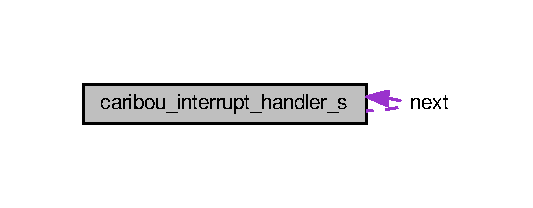
\includegraphics[width=256pt]{structcaribou__interrupt__handler__s__coll__graph}
\end{center}
\end{figure}
\subsection*{Data Fields}
\begin{DoxyCompactItemize}
\item 
\hyperlink{interrupt_8h_af609f1916308a4ac8148b51cad03f620}{caribou\-\_\-isr\-\_\-t} \hyperlink{structcaribou__interrupt__handler__s_aecb54a9629094e45d0de339021c6a1a0}{isr}
\item 
void $\ast$ \hyperlink{structcaribou__interrupt__handler__s_aefaec04418af509f17589f6e3ed6ff0e}{arg}
\item 
struct \\*
\hyperlink{structcaribou__interrupt__handler__s}{caribou\-\_\-interrupt\-\_\-handler\-\_\-s} $\ast$ \hyperlink{structcaribou__interrupt__handler__s_a0d58e1ee1f99080457360177c803b034}{next}
\end{DoxyCompactItemize}


\subsection{Detailed Description}


Definition at line 18 of file interrupt.\-c.



\subsection{Field Documentation}
\hypertarget{structcaribou__interrupt__handler__s_aefaec04418af509f17589f6e3ed6ff0e}{\index{caribou\-\_\-interrupt\-\_\-handler\-\_\-s@{caribou\-\_\-interrupt\-\_\-handler\-\_\-s}!arg@{arg}}
\index{arg@{arg}!caribou_interrupt_handler_s@{caribou\-\_\-interrupt\-\_\-handler\-\_\-s}}
\subsubsection[{arg}]{\setlength{\rightskip}{0pt plus 5cm}void$\ast$ caribou\-\_\-interrupt\-\_\-handler\-\_\-s\-::arg}}\label{structcaribou__interrupt__handler__s_aefaec04418af509f17589f6e3ed6ff0e}


Definition at line 21 of file interrupt.\-c.

\hypertarget{structcaribou__interrupt__handler__s_aecb54a9629094e45d0de339021c6a1a0}{\index{caribou\-\_\-interrupt\-\_\-handler\-\_\-s@{caribou\-\_\-interrupt\-\_\-handler\-\_\-s}!isr@{isr}}
\index{isr@{isr}!caribou_interrupt_handler_s@{caribou\-\_\-interrupt\-\_\-handler\-\_\-s}}
\subsubsection[{isr}]{\setlength{\rightskip}{0pt plus 5cm}{\bf caribou\-\_\-isr\-\_\-t} caribou\-\_\-interrupt\-\_\-handler\-\_\-s\-::isr}}\label{structcaribou__interrupt__handler__s_aecb54a9629094e45d0de339021c6a1a0}


Definition at line 20 of file interrupt.\-c.

\hypertarget{structcaribou__interrupt__handler__s_a0d58e1ee1f99080457360177c803b034}{\index{caribou\-\_\-interrupt\-\_\-handler\-\_\-s@{caribou\-\_\-interrupt\-\_\-handler\-\_\-s}!next@{next}}
\index{next@{next}!caribou_interrupt_handler_s@{caribou\-\_\-interrupt\-\_\-handler\-\_\-s}}
\subsubsection[{next}]{\setlength{\rightskip}{0pt plus 5cm}struct {\bf caribou\-\_\-interrupt\-\_\-handler\-\_\-s}$\ast$ caribou\-\_\-interrupt\-\_\-handler\-\_\-s\-::next}}\label{structcaribou__interrupt__handler__s_a0d58e1ee1f99080457360177c803b034}


Definition at line 22 of file interrupt.\-c.



The documentation for this struct was generated from the following file\-:\begin{DoxyCompactItemize}
\item 
src/kernel/\hyperlink{interrupt_8c}{interrupt.\-c}\end{DoxyCompactItemize}

\hypertarget{structcaribou__mutex__t}{\section{caribou\-\_\-mutex\-\_\-t Struct Reference}
\label{structcaribou__mutex__t}\index{caribou\-\_\-mutex\-\_\-t@{caribou\-\_\-mutex\-\_\-t}}
}


{\ttfamily \#include $<$mutex.\-h$>$}

\subsection*{Data Fields}
\begin{DoxyCompactItemize}
\item 
void $\ast$ \hyperlink{structcaribou__mutex__t_aa286035f1540359f0cd4f0de4a127304}{thread}
\item 
uint16\-\_\-t \hyperlink{structcaribou__mutex__t_ab4553f4d515724806d7f1bc90f8a0872}{locks}
\item 
uint8\-\_\-t \hyperlink{structcaribou__mutex__t_aa263fae88561085ee83fde049b400351}{flags}
\item 
uint8\-\_\-t \hyperlink{structcaribou__mutex__t_a58c4476d2113705569509e239501ae86}{blocking}
\end{DoxyCompactItemize}


\subsection{Detailed Description}


Definition at line 30 of file mutex.\-h.



\subsection{Field Documentation}
\hypertarget{structcaribou__mutex__t_a58c4476d2113705569509e239501ae86}{\index{caribou\-\_\-mutex\-\_\-t@{caribou\-\_\-mutex\-\_\-t}!blocking@{blocking}}
\index{blocking@{blocking}!caribou_mutex_t@{caribou\-\_\-mutex\-\_\-t}}
\subsubsection[{blocking}]{\setlength{\rightskip}{0pt plus 5cm}uint8\-\_\-t caribou\-\_\-mutex\-\_\-t\-::blocking}}\label{structcaribou__mutex__t_a58c4476d2113705569509e239501ae86}


Definition at line 35 of file mutex.\-h.

\hypertarget{structcaribou__mutex__t_aa263fae88561085ee83fde049b400351}{\index{caribou\-\_\-mutex\-\_\-t@{caribou\-\_\-mutex\-\_\-t}!flags@{flags}}
\index{flags@{flags}!caribou_mutex_t@{caribou\-\_\-mutex\-\_\-t}}
\subsubsection[{flags}]{\setlength{\rightskip}{0pt plus 5cm}uint8\-\_\-t caribou\-\_\-mutex\-\_\-t\-::flags}}\label{structcaribou__mutex__t_aa263fae88561085ee83fde049b400351}


Definition at line 34 of file mutex.\-h.

\hypertarget{structcaribou__mutex__t_ab4553f4d515724806d7f1bc90f8a0872}{\index{caribou\-\_\-mutex\-\_\-t@{caribou\-\_\-mutex\-\_\-t}!locks@{locks}}
\index{locks@{locks}!caribou_mutex_t@{caribou\-\_\-mutex\-\_\-t}}
\subsubsection[{locks}]{\setlength{\rightskip}{0pt plus 5cm}uint16\-\_\-t caribou\-\_\-mutex\-\_\-t\-::locks}}\label{structcaribou__mutex__t_ab4553f4d515724806d7f1bc90f8a0872}


Definition at line 33 of file mutex.\-h.

\hypertarget{structcaribou__mutex__t_aa286035f1540359f0cd4f0de4a127304}{\index{caribou\-\_\-mutex\-\_\-t@{caribou\-\_\-mutex\-\_\-t}!thread@{thread}}
\index{thread@{thread}!caribou_mutex_t@{caribou\-\_\-mutex\-\_\-t}}
\subsubsection[{thread}]{\setlength{\rightskip}{0pt plus 5cm}void$\ast$ caribou\-\_\-mutex\-\_\-t\-::thread}}\label{structcaribou__mutex__t_aa286035f1540359f0cd4f0de4a127304}


Definition at line 32 of file mutex.\-h.



The documentation for this struct was generated from the following file\-:\begin{DoxyCompactItemize}
\item 
include/caribou/lib/\hyperlink{mutex_8h}{mutex.\-h}\end{DoxyCompactItemize}

\hypertarget{structcaribou__spi__t}{\section{caribou\-\_\-spi\-\_\-t Struct Reference}
\label{structcaribou__spi__t}\index{caribou\-\_\-spi\-\_\-t@{caribou\-\_\-spi\-\_\-t}}
}


{\ttfamily \#include $<$spi.\-h$>$}

\subsection*{Data Fields}
\begin{DoxyCompactItemize}
\item 
chip\-\_\-spi\-\_\-port\-\_\-t \hyperlink{structcaribou__spi__t_ae1a7630daa892755a8a38a6e9cc8061c}{port}
\end{DoxyCompactItemize}


\subsection{Detailed Description}


Definition at line 26 of file spi.\-h.



\subsection{Field Documentation}
\hypertarget{structcaribou__spi__t_ae1a7630daa892755a8a38a6e9cc8061c}{\index{caribou\-\_\-spi\-\_\-t@{caribou\-\_\-spi\-\_\-t}!port@{port}}
\index{port@{port}!caribou_spi_t@{caribou\-\_\-spi\-\_\-t}}
\subsubsection[{port}]{\setlength{\rightskip}{0pt plus 5cm}chip\-\_\-spi\-\_\-port\-\_\-t caribou\-\_\-spi\-\_\-t\-::port}}\label{structcaribou__spi__t_ae1a7630daa892755a8a38a6e9cc8061c}


Definition at line 28 of file spi.\-h.



The documentation for this struct was generated from the following file\-:\begin{DoxyCompactItemize}
\item 
include/caribou/dev/\hyperlink{spi_8h}{spi.\-h}\end{DoxyCompactItemize}

\hypertarget{structcaribou__uart__config__t}{\section{caribou\-\_\-uart\-\_\-config\-\_\-t Struct Reference}
\label{structcaribou__uart__config__t}\index{caribou\-\_\-uart\-\_\-config\-\_\-t@{caribou\-\_\-uart\-\_\-config\-\_\-t}}
}


{\ttfamily \#include $<$uart.\-h$>$}

\subsection*{Data Fields}
\begin{DoxyCompactItemize}
\item 
\hyperlink{uart_8h_afef1566c0e2499ac54d03f9840e67367}{caribou\-\_\-uart\-\_\-baud\-\_\-t} \hyperlink{structcaribou__uart__config__t_a6138aeea535f2b07ffe791cf77805e78}{baud\-\_\-rate}
\item 
\hyperlink{uart_8h_a9a6df27e70711dcf554553bcd934cdf9}{caribou\-\_\-uart\-\_\-word\-\_\-t} \hyperlink{structcaribou__uart__config__t_a89d25d0eefe1f3856ccc6568026e00b1}{word\-\_\-size}
\item 
\hyperlink{uart_8h_a8a7a8a9e91ed00784943f12dd2b3825e}{caribou\-\_\-uart\-\_\-stop\-\_\-t} \hyperlink{structcaribou__uart__config__t_a9489f3e6667476da945ac8b99543e9c0}{stop\-\_\-bits}
\item 
\hyperlink{uart_8h_a21331436e5b880d78970abb6dbfad09b}{caribou\-\_\-uart\-\_\-parity\-\_\-t} \hyperlink{structcaribou__uart__config__t_aeb5a0f9cc2e23070859bcb7033777e14}{parity\-\_\-bits}
\item 
\hyperlink{uart_8h_a54948edc934015197b158136f30a074d}{caribou\-\_\-uart\-\_\-flow\-\_\-t} \hyperlink{structcaribou__uart__config__t_a94d7122367d7664b02df609cbae278c2}{flow\-\_\-control}
\item 
\hyperlink{uart_8h_abc83350727ee87e6056c52670ef81707}{caribou\-\_\-uart\-\_\-dma\-\_\-t} \hyperlink{structcaribou__uart__config__t_a257b346e7b980b0f2b089f27cc54569d}{dma\-\_\-mode}
\end{DoxyCompactItemize}


\subsection{Detailed Description}


Definition at line 127 of file uart.\-h.



\subsection{Field Documentation}
\hypertarget{structcaribou__uart__config__t_a6138aeea535f2b07ffe791cf77805e78}{\index{caribou\-\_\-uart\-\_\-config\-\_\-t@{caribou\-\_\-uart\-\_\-config\-\_\-t}!baud\-\_\-rate@{baud\-\_\-rate}}
\index{baud\-\_\-rate@{baud\-\_\-rate}!caribou_uart_config_t@{caribou\-\_\-uart\-\_\-config\-\_\-t}}
\subsubsection[{baud\-\_\-rate}]{\setlength{\rightskip}{0pt plus 5cm}{\bf caribou\-\_\-uart\-\_\-baud\-\_\-t} caribou\-\_\-uart\-\_\-config\-\_\-t\-::baud\-\_\-rate}}\label{structcaribou__uart__config__t_a6138aeea535f2b07ffe791cf77805e78}


Definition at line 129 of file uart.\-h.

\hypertarget{structcaribou__uart__config__t_a257b346e7b980b0f2b089f27cc54569d}{\index{caribou\-\_\-uart\-\_\-config\-\_\-t@{caribou\-\_\-uart\-\_\-config\-\_\-t}!dma\-\_\-mode@{dma\-\_\-mode}}
\index{dma\-\_\-mode@{dma\-\_\-mode}!caribou_uart_config_t@{caribou\-\_\-uart\-\_\-config\-\_\-t}}
\subsubsection[{dma\-\_\-mode}]{\setlength{\rightskip}{0pt plus 5cm}{\bf caribou\-\_\-uart\-\_\-dma\-\_\-t} caribou\-\_\-uart\-\_\-config\-\_\-t\-::dma\-\_\-mode}}\label{structcaribou__uart__config__t_a257b346e7b980b0f2b089f27cc54569d}


Definition at line 134 of file uart.\-h.

\hypertarget{structcaribou__uart__config__t_a94d7122367d7664b02df609cbae278c2}{\index{caribou\-\_\-uart\-\_\-config\-\_\-t@{caribou\-\_\-uart\-\_\-config\-\_\-t}!flow\-\_\-control@{flow\-\_\-control}}
\index{flow\-\_\-control@{flow\-\_\-control}!caribou_uart_config_t@{caribou\-\_\-uart\-\_\-config\-\_\-t}}
\subsubsection[{flow\-\_\-control}]{\setlength{\rightskip}{0pt plus 5cm}{\bf caribou\-\_\-uart\-\_\-flow\-\_\-t} caribou\-\_\-uart\-\_\-config\-\_\-t\-::flow\-\_\-control}}\label{structcaribou__uart__config__t_a94d7122367d7664b02df609cbae278c2}


Definition at line 133 of file uart.\-h.

\hypertarget{structcaribou__uart__config__t_aeb5a0f9cc2e23070859bcb7033777e14}{\index{caribou\-\_\-uart\-\_\-config\-\_\-t@{caribou\-\_\-uart\-\_\-config\-\_\-t}!parity\-\_\-bits@{parity\-\_\-bits}}
\index{parity\-\_\-bits@{parity\-\_\-bits}!caribou_uart_config_t@{caribou\-\_\-uart\-\_\-config\-\_\-t}}
\subsubsection[{parity\-\_\-bits}]{\setlength{\rightskip}{0pt plus 5cm}{\bf caribou\-\_\-uart\-\_\-parity\-\_\-t} caribou\-\_\-uart\-\_\-config\-\_\-t\-::parity\-\_\-bits}}\label{structcaribou__uart__config__t_aeb5a0f9cc2e23070859bcb7033777e14}


Definition at line 132 of file uart.\-h.

\hypertarget{structcaribou__uart__config__t_a9489f3e6667476da945ac8b99543e9c0}{\index{caribou\-\_\-uart\-\_\-config\-\_\-t@{caribou\-\_\-uart\-\_\-config\-\_\-t}!stop\-\_\-bits@{stop\-\_\-bits}}
\index{stop\-\_\-bits@{stop\-\_\-bits}!caribou_uart_config_t@{caribou\-\_\-uart\-\_\-config\-\_\-t}}
\subsubsection[{stop\-\_\-bits}]{\setlength{\rightskip}{0pt plus 5cm}{\bf caribou\-\_\-uart\-\_\-stop\-\_\-t} caribou\-\_\-uart\-\_\-config\-\_\-t\-::stop\-\_\-bits}}\label{structcaribou__uart__config__t_a9489f3e6667476da945ac8b99543e9c0}


Definition at line 131 of file uart.\-h.

\hypertarget{structcaribou__uart__config__t_a89d25d0eefe1f3856ccc6568026e00b1}{\index{caribou\-\_\-uart\-\_\-config\-\_\-t@{caribou\-\_\-uart\-\_\-config\-\_\-t}!word\-\_\-size@{word\-\_\-size}}
\index{word\-\_\-size@{word\-\_\-size}!caribou_uart_config_t@{caribou\-\_\-uart\-\_\-config\-\_\-t}}
\subsubsection[{word\-\_\-size}]{\setlength{\rightskip}{0pt plus 5cm}{\bf caribou\-\_\-uart\-\_\-word\-\_\-t} caribou\-\_\-uart\-\_\-config\-\_\-t\-::word\-\_\-size}}\label{structcaribou__uart__config__t_a89d25d0eefe1f3856ccc6568026e00b1}


Definition at line 130 of file uart.\-h.



The documentation for this struct was generated from the following file\-:\begin{DoxyCompactItemize}
\item 
include/caribou/dev/\hyperlink{uart_8h}{uart.\-h}\end{DoxyCompactItemize}

\hypertarget{structheap__tag}{\section{heap\-\_\-tag Struct Reference}
\label{structheap__tag}\index{heap\-\_\-tag@{heap\-\_\-tag}}
}


Collaboration diagram for heap\-\_\-tag\-:
\nopagebreak
\begin{figure}[H]
\begin{center}
\leavevmode
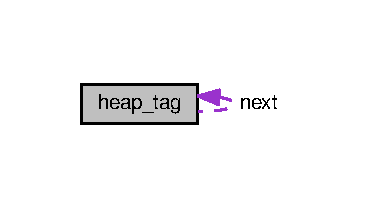
\includegraphics[width=175pt]{structheap__tag__coll__graph}
\end{center}
\end{figure}
\subsection*{Data Fields}
\begin{DoxyCompactItemize}
\item 
struct \hyperlink{structheap__tag}{heap\-\_\-tag} $\ast$ \hyperlink{structheap__tag_ae0e42d810512a9636393bab081921a7c}{next}
\item 
size\-\_\-t \hyperlink{structheap__tag_aa492677962c3d48df0880c9dacea3564}{size}
\end{DoxyCompactItemize}


\subsection{Detailed Description}


Definition at line 19 of file nova\-\_\-heap.\-c.



\subsection{Field Documentation}
\hypertarget{structheap__tag_ae0e42d810512a9636393bab081921a7c}{\index{heap\-\_\-tag@{heap\-\_\-tag}!next@{next}}
\index{next@{next}!heap_tag@{heap\-\_\-tag}}
\subsubsection[{next}]{\setlength{\rightskip}{0pt plus 5cm}struct {\bf heap\-\_\-tag}$\ast$ heap\-\_\-tag\-::next}}\label{structheap__tag_ae0e42d810512a9636393bab081921a7c}


Definition at line 21 of file nova\-\_\-heap.\-c.

\hypertarget{structheap__tag_aa492677962c3d48df0880c9dacea3564}{\index{heap\-\_\-tag@{heap\-\_\-tag}!size@{size}}
\index{size@{size}!heap_tag@{heap\-\_\-tag}}
\subsubsection[{size}]{\setlength{\rightskip}{0pt plus 5cm}size\-\_\-t heap\-\_\-tag\-::size}}\label{structheap__tag_aa492677962c3d48df0880c9dacea3564}


Definition at line 22 of file nova\-\_\-heap.\-c.



The documentation for this struct was generated from the following file\-:\begin{DoxyCompactItemize}
\item 
src/lib/\hyperlink{nova__heap_8c}{nova\-\_\-heap.\-c}\end{DoxyCompactItemize}

\hypertarget{unionieee__double__shape__type}{\section{ieee\-\_\-double\-\_\-shape\-\_\-type Union Reference}
\label{unionieee__double__shape__type}\index{ieee\-\_\-double\-\_\-shape\-\_\-type@{ieee\-\_\-double\-\_\-shape\-\_\-type}}
}


{\ttfamily \#include $<$math\-\_\-private.\-h$>$}

\subsection*{Data Fields}
\begin{DoxyCompactItemize}
\item 
double \hyperlink{unionieee__double__shape__type_a2d9c4cab9e3fa74e4be6d72f798a145b}{value}
\item 
\begin{tabbing}
xx\=xx\=xx\=xx\=xx\=xx\=xx\=xx\=xx\=\kill
struct \{\\
\>uint32\_t \hyperlink{unionieee__double__shape__type_a887ac49e741cafa9c74aa397a6fa04a5}{msw}\\
\>uint32\_t \hyperlink{unionieee__double__shape__type_a31323ff275e4b9f21d1f0dac6ed02a97}{lsw}\\
\} \hyperlink{unionieee__double__shape__type_a56d56a067ef071ada93836397ea0050a}{parts}\\

\end{tabbing}\item 
\begin{tabbing}
xx\=xx\=xx\=xx\=xx\=xx\=xx\=xx\=xx\=\kill
struct \{\\
\>uint32\_t \hyperlink{unionieee__double__shape__type_a31323ff275e4b9f21d1f0dac6ed02a97}{lsw}\\
\>uint32\_t \hyperlink{unionieee__double__shape__type_a887ac49e741cafa9c74aa397a6fa04a5}{msw}\\
\} \hyperlink{unionieee__double__shape__type_a14b6183c096c0f76d6596e3c737d3c9b}{parts}\\

\end{tabbing}\end{DoxyCompactItemize}


\subsection{Detailed Description}


Definition at line 20 of file math\-\_\-private.\-h.



\subsection{Field Documentation}
\hypertarget{unionieee__double__shape__type_a31323ff275e4b9f21d1f0dac6ed02a97}{\index{ieee\-\_\-double\-\_\-shape\-\_\-type@{ieee\-\_\-double\-\_\-shape\-\_\-type}!lsw@{lsw}}
\index{lsw@{lsw}!ieee_double_shape_type@{ieee\-\_\-double\-\_\-shape\-\_\-type}}
\subsubsection[{lsw}]{\setlength{\rightskip}{0pt plus 5cm}uint32\-\_\-t ieee\-\_\-double\-\_\-shape\-\_\-type\-::lsw}}\label{unionieee__double__shape__type_a31323ff275e4b9f21d1f0dac6ed02a97}


Definition at line 26 of file math\-\_\-private.\-h.

\hypertarget{unionieee__double__shape__type_a887ac49e741cafa9c74aa397a6fa04a5}{\index{ieee\-\_\-double\-\_\-shape\-\_\-type@{ieee\-\_\-double\-\_\-shape\-\_\-type}!msw@{msw}}
\index{msw@{msw}!ieee_double_shape_type@{ieee\-\_\-double\-\_\-shape\-\_\-type}}
\subsubsection[{msw}]{\setlength{\rightskip}{0pt plus 5cm}uint32\-\_\-t ieee\-\_\-double\-\_\-shape\-\_\-type\-::msw}}\label{unionieee__double__shape__type_a887ac49e741cafa9c74aa397a6fa04a5}


Definition at line 25 of file math\-\_\-private.\-h.

\hypertarget{unionieee__double__shape__type_a56d56a067ef071ada93836397ea0050a}{\index{ieee\-\_\-double\-\_\-shape\-\_\-type@{ieee\-\_\-double\-\_\-shape\-\_\-type}!parts@{parts}}
\index{parts@{parts}!ieee_double_shape_type@{ieee\-\_\-double\-\_\-shape\-\_\-type}}
\subsubsection[{parts}]{\setlength{\rightskip}{0pt plus 5cm}struct \{ ... \}   ieee\-\_\-double\-\_\-shape\-\_\-type\-::parts}}\label{unionieee__double__shape__type_a56d56a067ef071ada93836397ea0050a}
\hypertarget{unionieee__double__shape__type_a14b6183c096c0f76d6596e3c737d3c9b}{\index{ieee\-\_\-double\-\_\-shape\-\_\-type@{ieee\-\_\-double\-\_\-shape\-\_\-type}!parts@{parts}}
\index{parts@{parts}!ieee_double_shape_type@{ieee\-\_\-double\-\_\-shape\-\_\-type}}
\subsubsection[{parts}]{\setlength{\rightskip}{0pt plus 5cm}struct \{ ... \}   ieee\-\_\-double\-\_\-shape\-\_\-type\-::parts}}\label{unionieee__double__shape__type_a14b6183c096c0f76d6596e3c737d3c9b}
\hypertarget{unionieee__double__shape__type_a2d9c4cab9e3fa74e4be6d72f798a145b}{\index{ieee\-\_\-double\-\_\-shape\-\_\-type@{ieee\-\_\-double\-\_\-shape\-\_\-type}!value@{value}}
\index{value@{value}!ieee_double_shape_type@{ieee\-\_\-double\-\_\-shape\-\_\-type}}
\subsubsection[{value}]{\setlength{\rightskip}{0pt plus 5cm}double ieee\-\_\-double\-\_\-shape\-\_\-type\-::value}}\label{unionieee__double__shape__type_a2d9c4cab9e3fa74e4be6d72f798a145b}


Definition at line 22 of file math\-\_\-private.\-h.



The documentation for this union was generated from the following file\-:\begin{DoxyCompactItemize}
\item 
include/caribou/lib/\hyperlink{math__private_8h}{math\-\_\-private.\-h}\end{DoxyCompactItemize}

\hypertarget{unionieee__float__shape__type}{\section{ieee\-\_\-float\-\_\-shape\-\_\-type Union Reference}
\label{unionieee__float__shape__type}\index{ieee\-\_\-float\-\_\-shape\-\_\-type@{ieee\-\_\-float\-\_\-shape\-\_\-type}}
}


{\ttfamily \#include $<$math\-\_\-private.\-h$>$}

\subsection*{Data Fields}
\begin{DoxyCompactItemize}
\item 
float \hyperlink{unionieee__float__shape__type_aa0c47451f1b974421cbb9e2833ddb68e}{value}
\item 
uint32\-\_\-t \hyperlink{unionieee__float__shape__type_adb70a477cb0179659bb95dc6b1870b80}{word}
\end{DoxyCompactItemize}


\subsection{Detailed Description}


Definition at line 109 of file math\-\_\-private.\-h.



\subsection{Field Documentation}
\hypertarget{unionieee__float__shape__type_aa0c47451f1b974421cbb9e2833ddb68e}{\index{ieee\-\_\-float\-\_\-shape\-\_\-type@{ieee\-\_\-float\-\_\-shape\-\_\-type}!value@{value}}
\index{value@{value}!ieee_float_shape_type@{ieee\-\_\-float\-\_\-shape\-\_\-type}}
\subsubsection[{value}]{\setlength{\rightskip}{0pt plus 5cm}float ieee\-\_\-float\-\_\-shape\-\_\-type\-::value}}\label{unionieee__float__shape__type_aa0c47451f1b974421cbb9e2833ddb68e}


Definition at line 111 of file math\-\_\-private.\-h.

\hypertarget{unionieee__float__shape__type_adb70a477cb0179659bb95dc6b1870b80}{\index{ieee\-\_\-float\-\_\-shape\-\_\-type@{ieee\-\_\-float\-\_\-shape\-\_\-type}!word@{word}}
\index{word@{word}!ieee_float_shape_type@{ieee\-\_\-float\-\_\-shape\-\_\-type}}
\subsubsection[{word}]{\setlength{\rightskip}{0pt plus 5cm}uint32\-\_\-t ieee\-\_\-float\-\_\-shape\-\_\-type\-::word}}\label{unionieee__float__shape__type_adb70a477cb0179659bb95dc6b1870b80}


Definition at line 112 of file math\-\_\-private.\-h.



The documentation for this union was generated from the following file\-:\begin{DoxyCompactItemize}
\item 
include/caribou/lib/\hyperlink{math__private_8h}{math\-\_\-private.\-h}\end{DoxyCompactItemize}

\chapter{File Documentation}
\hypertarget{caribou_8h}{\section{include/caribou.h File Reference}
\label{caribou_8h}\index{include/caribou.\-h@{include/caribou.\-h}}
}
{\ttfamily \#include $<$caribou\-\_\-config.\-h$>$}\\*
{\ttfamily \#include $<$board.\-h$>$}\\*
{\ttfamily \#include $<$caribou/kernel/types.\-h$>$}\\*
{\ttfamily \#include $<$caribou/kernel/timer.\-h$>$}\\*
{\ttfamily \#include $<$caribou/kernel/thread.\-h$>$}\\*
{\ttfamily \#include $<$caribou/kernel/interrupt.\-h$>$}\\*
{\ttfamily \#include $<$caribou/lib/bytequeue.\-h$>$}\\*
{\ttfamily \#include $<$caribou/lib/cbmath.\-h$>$}\\*
{\ttfamily \#include $<$caribou/lib/errno.\-h$>$}\\*
{\ttfamily \#include $<$caribou/lib/fault.\-h$>$}\\*
{\ttfamily \#include $<$caribou/lib/heap.\-h$>$}\\*
{\ttfamily \#include $<$caribou/lib/mutex.\-h$>$}\\*
{\ttfamily \#include $<$caribou/lib/qsort.\-h$>$}\\*
{\ttfamily \#include $<$caribou/lib/queue.\-h$>$}\\*
{\ttfamily \#include $<$caribou/lib/rand.\-h$>$}\\*
{\ttfamily \#include $<$caribou/lib/semaphore.\-h$>$}\\*
{\ttfamily \#include $<$caribou/lib/spinlock.\-h$>$}\\*
{\ttfamily \#include $<$caribou/lib/stdarg.\-h$>$}\\*
{\ttfamily \#include $<$caribou/lib/stddef.\-h$>$}\\*
{\ttfamily \#include $<$caribou/lib/stdint.\-h$>$}\\*
{\ttfamily \#include $<$caribou/lib/stdio.\-h$>$}\\*
{\ttfamily \#include $<$caribou/lib/string.\-h$>$}\\*
{\ttfamily \#include $<$caribou/dev/adc.\-h$>$}\\*
{\ttfamily \#include $<$caribou/dev/gpio.\-h$>$}\\*
{\ttfamily \#include $<$caribou/dev/i2c.\-h$>$}\\*
{\ttfamily \#include $<$caribou/dev/i2s.\-h$>$}\\*
{\ttfamily \#include $<$caribou/dev/spi.\-h$>$}\\*
{\ttfamily \#include $<$caribou/dev/uart.\-h$>$}\\*
Include dependency graph for caribou.\-h\-:
\nopagebreak
\begin{figure}[H]
\begin{center}
\leavevmode
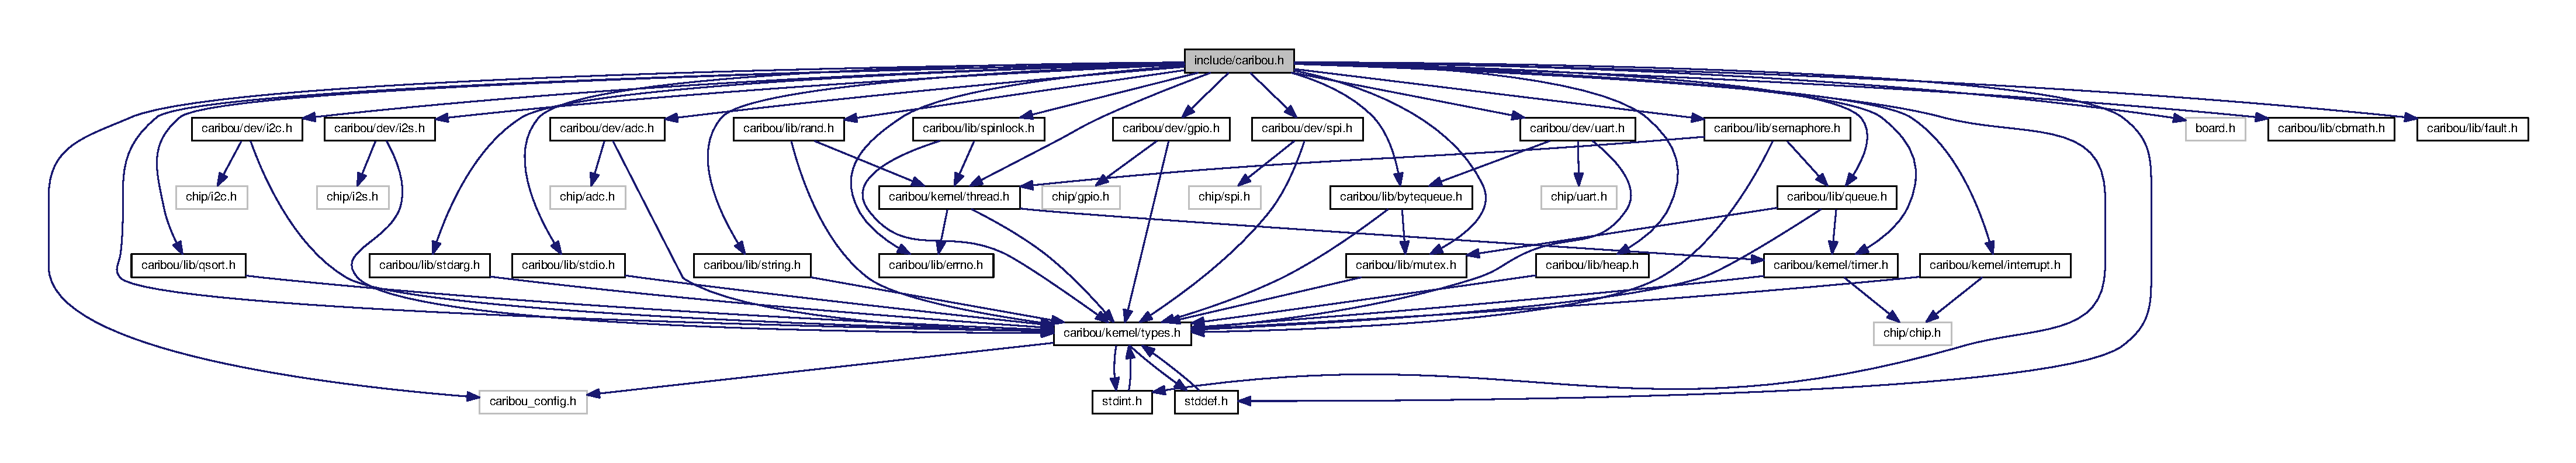
\includegraphics[width=350pt]{caribou_8h__incl}
\end{center}
\end{figure}
This graph shows which files directly or indirectly include this file\-:\nopagebreak
\begin{figure}[H]
\begin{center}
\leavevmode
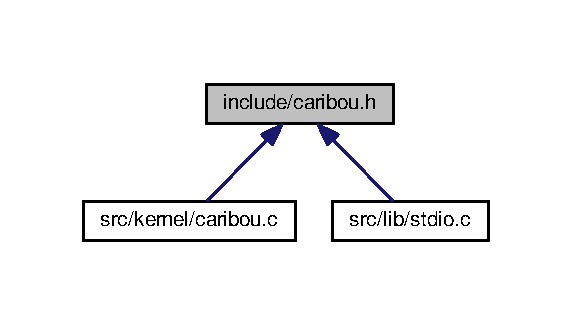
\includegraphics[width=274pt]{caribou_8h__dep__incl}
\end{center}
\end{figure}
\subsection*{Macros}
\begin{DoxyCompactItemize}
\item 
\#define \hyperlink{caribou_8h_a03be0a0963032234feb3085823fe242f}{\-\_\-\-\_\-\-C\-A\-R\-I\-B\-O\-U\-\_\-\-R\-T\-O\-S\-\_\-\-\_\-}
\item 
\#define \hyperlink{caribou_8h_a71f641a08d4d7a6a12e4f686d30fc1ad}{C\-A\-R\-I\-B\-O\-U\-\_\-\-V\-E\-R\-S\-I\-O\-N}~\char`\"{}0.\-9.\-5\char`\"{}
\end{DoxyCompactItemize}
\subsection*{Functions}
\begin{DoxyCompactItemize}
\item 
int \hyperlink{caribou_8h_ae9efd2bf2874e10d63a5cf40bf33802c}{caribou\-\_\-lock\-\_\-state} ()
\begin{DoxyCompactList}\small\item\em Test the state of the C\-A\-R\-I\-B\-O\-U scheduler lock. \end{DoxyCompactList}\item 
int \hyperlink{caribou_8h_a3f6b11e983ac91165a6fd14d35aed51f}{caribou\-\_\-lock} ()
\begin{DoxyCompactList}\small\item\em Lock the C\-A\-R\-I\-B\-O\-U scheduler onto current thread. \end{DoxyCompactList}\item 
int \hyperlink{caribou_8h_ae6fc3a012fed78adc9a36933057c857f}{caribou\-\_\-unlock} ()
\begin{DoxyCompactList}\small\item\em Unlock the C\-A\-R\-I\-B\-O\-U scheduler. \end{DoxyCompactList}\item 
void \hyperlink{caribou_8h_aa8627675e0c04813d45817fda119c5dc}{caribou\-\_\-lock\-\_\-set} (int state)
\begin{DoxyCompactList}\small\item\em Set the C\-A\-R\-I\-B\-O\-U scheduler lock state. \end{DoxyCompactList}\item 
void \hyperlink{caribou_8h_a8c39159ad641e81210c3307ab7d64227}{caribou\-\_\-preempt} ()
\begin{DoxyCompactList}\small\item\em Force scheduler to perform a context switch. \end{DoxyCompactList}\item 
void \hyperlink{caribou_8h_a9a6ffa8babf5f0ea286bda1e464d7623}{caribou\-\_\-exec} (void)
\begin{DoxyCompactList}\small\item\em The C\-A\-R\-I\-B\-O\-U main thread loop. \hyperlink{caribou_8c_a9a6ffa8babf5f0ea286bda1e464d7623}{caribou\-\_\-exec()} does not return. \end{DoxyCompactList}\item 
void \hyperlink{caribou_8h_a2d4f021763a6e4c2918ef9f4285d9585}{caribou\-\_\-init\-\_\-clock} ()
\begin{DoxyCompactList}\small\item\em Initialize the clock such that jiffies start ticking. \end{DoxyCompactList}\item 
void \hyperlink{caribou_8h_a586f22d1e2495896b4345fa5652e06c9}{caribou\-\_\-init} (int8\-\_\-t priority)
\begin{DoxyCompactList}\small\item\em Initialize the C\-A\-R\-I\-B\-O\-U main thread. \end{DoxyCompactList}\item 
const char $\ast$ \hyperlink{caribou_8h_a2eb1e1c5f0f424d820818c92cf3ea0a1}{caribou\-\_\-version} ()
\item 
void \hyperlink{caribou_8h_a1a217e5e2edbe64ce64925d387a49c63}{caribou\-\_\-early\-\_\-init} (void)
\begin{DoxyCompactList}\small\item\em A hook to perform early board initialization. Static stacks are initialized, B\-S\-S is {\itshape N\-O\-T} initialized at this stage. \end{DoxyCompactList}\item 
void \hyperlink{caribou_8h_af0bfafa240382bfab4ee9c3279b75b8c}{caribou\-\_\-late\-\_\-init} (void)
\begin{DoxyCompactList}\small\item\em A hook to perform late initialization. Static stacks, B\-S\-S, heap, and static contructors are all initialized at this stage. \end{DoxyCompactList}\end{DoxyCompactItemize}


\subsection{Detailed Description}




\begin{DoxyAuthor}{Author}
Mike Sharkey \href{mailto:mike@pikeaero.com}{\tt mike@pikeaero.\-com}. 
\end{DoxyAuthor}
\begin{DoxyCopyright}{Copyright}
© 2005-\/2013 by Pike Aerospace Research Corporation 

© 2014-\/2015 by Mike Sharkey
\end{DoxyCopyright}
This file is part of C\-A\-R\-I\-B\-O\-U R\-T\-O\-S C\-A\-R\-I\-B\-O\-U R\-T\-O\-S is free software\-: you can redistribute it and/or modify it under the terms of the Beerware License Version 43. \char`\"{}\-T\-H\-E B\-E\-E\-R-\/\-W\-A\-R\-E L\-I\-C\-E\-N\-S\-E\char`\"{} (Revision 43)\-: Mike Sharkey \href{mailto:mike@pikeaero.com}{\tt mike@pikeaero.\-com} wrote this file. As long as you retain this notice you can do whatever you want with this stuff. If we meet some day, and you think this stuff is worth it, you can buy me a beer in return $\sim$ Mike Sharkey 

Definition in file \hyperlink{caribou_8h_source}{caribou.\-h}.



\subsection{Macro Definition Documentation}
\hypertarget{caribou_8h_a03be0a0963032234feb3085823fe242f}{\index{caribou.\-h@{caribou.\-h}!\-\_\-\-\_\-\-C\-A\-R\-I\-B\-O\-U\-\_\-\-R\-T\-O\-S\-\_\-\-\_\-@{\-\_\-\-\_\-\-C\-A\-R\-I\-B\-O\-U\-\_\-\-R\-T\-O\-S\-\_\-\-\_\-}}
\index{\-\_\-\-\_\-\-C\-A\-R\-I\-B\-O\-U\-\_\-\-R\-T\-O\-S\-\_\-\-\_\-@{\-\_\-\-\_\-\-C\-A\-R\-I\-B\-O\-U\-\_\-\-R\-T\-O\-S\-\_\-\-\_\-}!caribou.h@{caribou.\-h}}
\subsubsection[{\-\_\-\-\_\-\-C\-A\-R\-I\-B\-O\-U\-\_\-\-R\-T\-O\-S\-\_\-\-\_\-}]{\setlength{\rightskip}{0pt plus 5cm}\#define \-\_\-\-\_\-\-C\-A\-R\-I\-B\-O\-U\-\_\-\-R\-T\-O\-S\-\_\-\-\_\-}}\label{caribou_8h_a03be0a0963032234feb3085823fe242f}


Definition at line 57 of file caribou.\-h.

\hypertarget{caribou_8h_a71f641a08d4d7a6a12e4f686d30fc1ad}{\index{caribou.\-h@{caribou.\-h}!C\-A\-R\-I\-B\-O\-U\-\_\-\-V\-E\-R\-S\-I\-O\-N@{C\-A\-R\-I\-B\-O\-U\-\_\-\-V\-E\-R\-S\-I\-O\-N}}
\index{C\-A\-R\-I\-B\-O\-U\-\_\-\-V\-E\-R\-S\-I\-O\-N@{C\-A\-R\-I\-B\-O\-U\-\_\-\-V\-E\-R\-S\-I\-O\-N}!caribou.h@{caribou.\-h}}
\subsubsection[{C\-A\-R\-I\-B\-O\-U\-\_\-\-V\-E\-R\-S\-I\-O\-N}]{\setlength{\rightskip}{0pt plus 5cm}\#define C\-A\-R\-I\-B\-O\-U\-\_\-\-V\-E\-R\-S\-I\-O\-N~\char`\"{}0.\-9.\-5\char`\"{}}}\label{caribou_8h_a71f641a08d4d7a6a12e4f686d30fc1ad}


Definition at line 60 of file caribou.\-h.



\subsection{Function Documentation}
\hypertarget{caribou_8h_a1a217e5e2edbe64ce64925d387a49c63}{\index{caribou.\-h@{caribou.\-h}!caribou\-\_\-early\-\_\-init@{caribou\-\_\-early\-\_\-init}}
\index{caribou\-\_\-early\-\_\-init@{caribou\-\_\-early\-\_\-init}!caribou.h@{caribou.\-h}}
\subsubsection[{caribou\-\_\-early\-\_\-init}]{\setlength{\rightskip}{0pt plus 5cm}void caribou\-\_\-early\-\_\-init (
\begin{DoxyParamCaption}
\item[{void}]{}
\end{DoxyParamCaption}
)}}\label{caribou_8h_a1a217e5e2edbe64ce64925d387a49c63}


A hook to perform early board initialization. Static stacks are initialized, B\-S\-S is {\itshape N\-O\-T} initialized at this stage. 

\hypertarget{caribou_8h_a9a6ffa8babf5f0ea286bda1e464d7623}{\index{caribou.\-h@{caribou.\-h}!caribou\-\_\-exec@{caribou\-\_\-exec}}
\index{caribou\-\_\-exec@{caribou\-\_\-exec}!caribou.h@{caribou.\-h}}
\subsubsection[{caribou\-\_\-exec}]{\setlength{\rightskip}{0pt plus 5cm}void caribou\-\_\-exec (
\begin{DoxyParamCaption}
\item[{void}]{}
\end{DoxyParamCaption}
)}}\label{caribou_8h_a9a6ffa8babf5f0ea286bda1e464d7623}


The C\-A\-R\-I\-B\-O\-U main thread loop. \hyperlink{caribou_8c_a9a6ffa8babf5f0ea286bda1e464d7623}{caribou\-\_\-exec()} does not return. 

\begin{DoxyNote}{Note}
If it is desired to run some application code from the main thread, then it is recommended that the application code implement the main\-\_\-idle() function which is callback from the main thread idle loop, and will be called after each cycle of C\-A\-R\-I\-B\-O\-U house keeping. 
\end{DoxyNote}
never to return. 

Definition at line 90 of file caribou.\-c.



Here is the call graph for this function\-:
\nopagebreak
\begin{figure}[H]
\begin{center}
\leavevmode
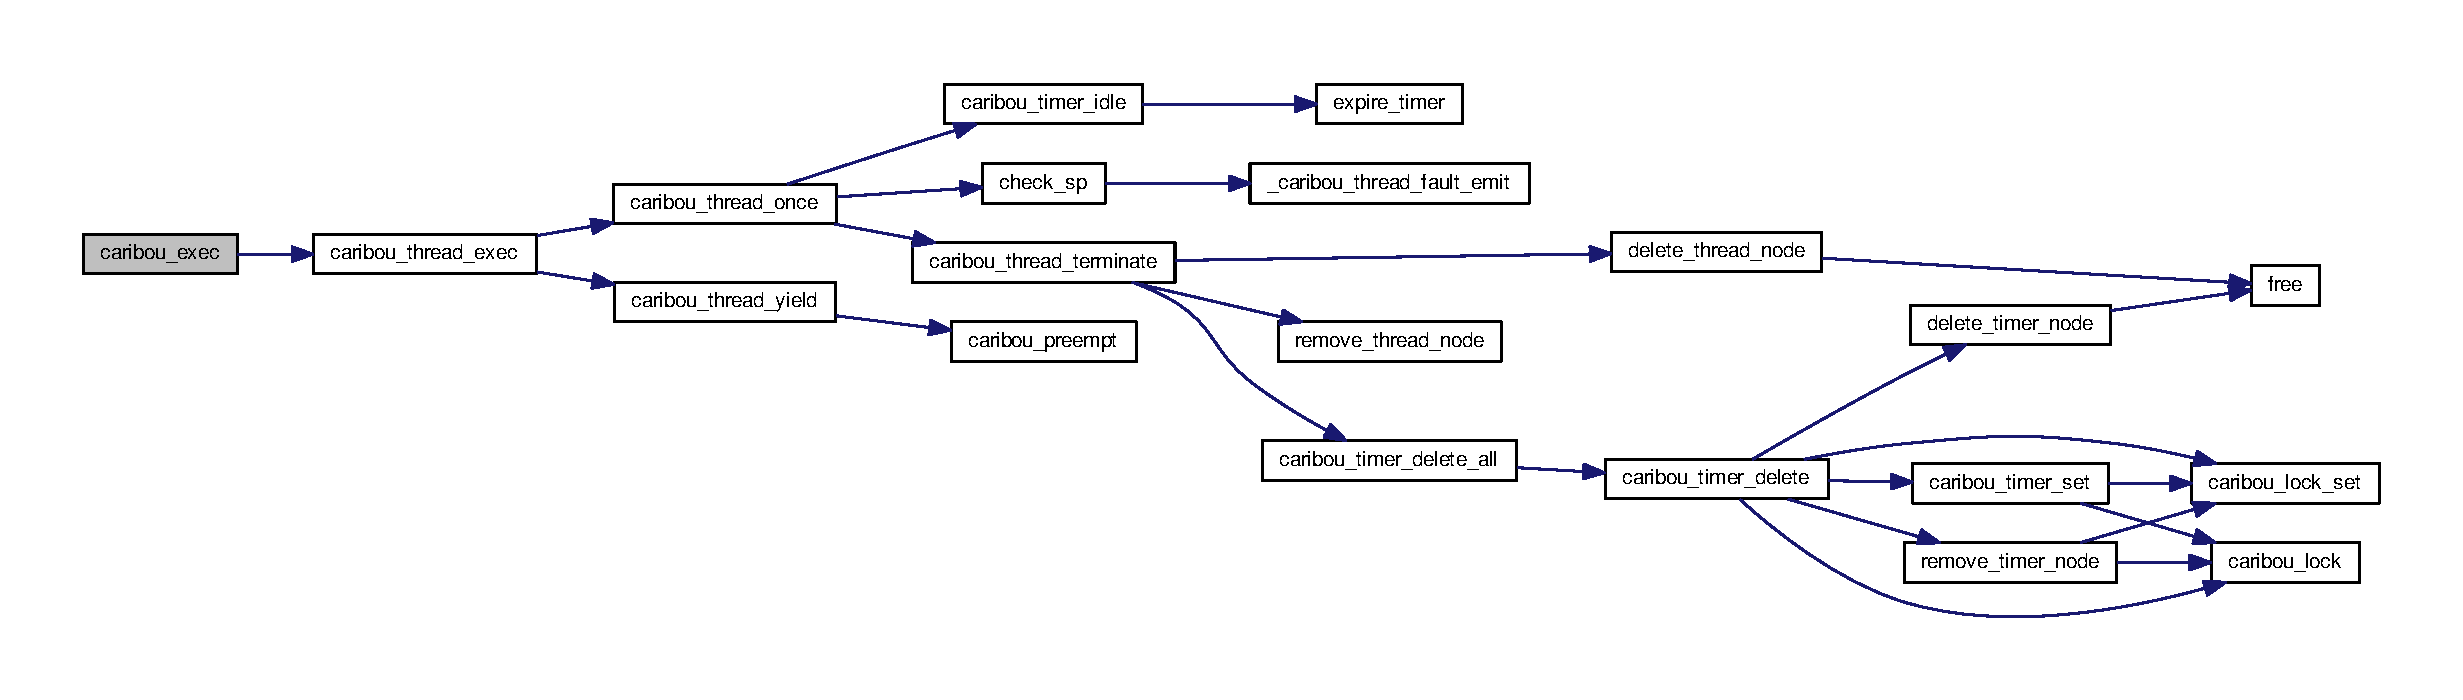
\includegraphics[width=350pt]{caribou_8h_a9a6ffa8babf5f0ea286bda1e464d7623_cgraph}
\end{center}
\end{figure}


\hypertarget{caribou_8h_a586f22d1e2495896b4345fa5652e06c9}{\index{caribou.\-h@{caribou.\-h}!caribou\-\_\-init@{caribou\-\_\-init}}
\index{caribou\-\_\-init@{caribou\-\_\-init}!caribou.h@{caribou.\-h}}
\subsubsection[{caribou\-\_\-init}]{\setlength{\rightskip}{0pt plus 5cm}void caribou\-\_\-init (
\begin{DoxyParamCaption}
\item[{int8\-\_\-t}]{priority}
\end{DoxyParamCaption}
)}}\label{caribou_8h_a586f22d1e2495896b4345fa5652e06c9}


Initialize the C\-A\-R\-I\-B\-O\-U main thread. 


\begin{DoxyParams}{Parameters}
{\em priority} & The priority to assign to the main thread. \\
\hline
\end{DoxyParams}
\begin{DoxyNote}{Note}
Interrupts are disabled for the duration of this function. 

\hyperlink{caribou_8c_a586f22d1e2495896b4345fa5652e06c9}{caribou\-\_\-init()} must be called before any other C\-A\-R\-I\-B\-O\-U threads are created. 
\end{DoxyNote}


Definition at line 115 of file caribou.\-c.



Here is the call graph for this function\-:
\nopagebreak
\begin{figure}[H]
\begin{center}
\leavevmode
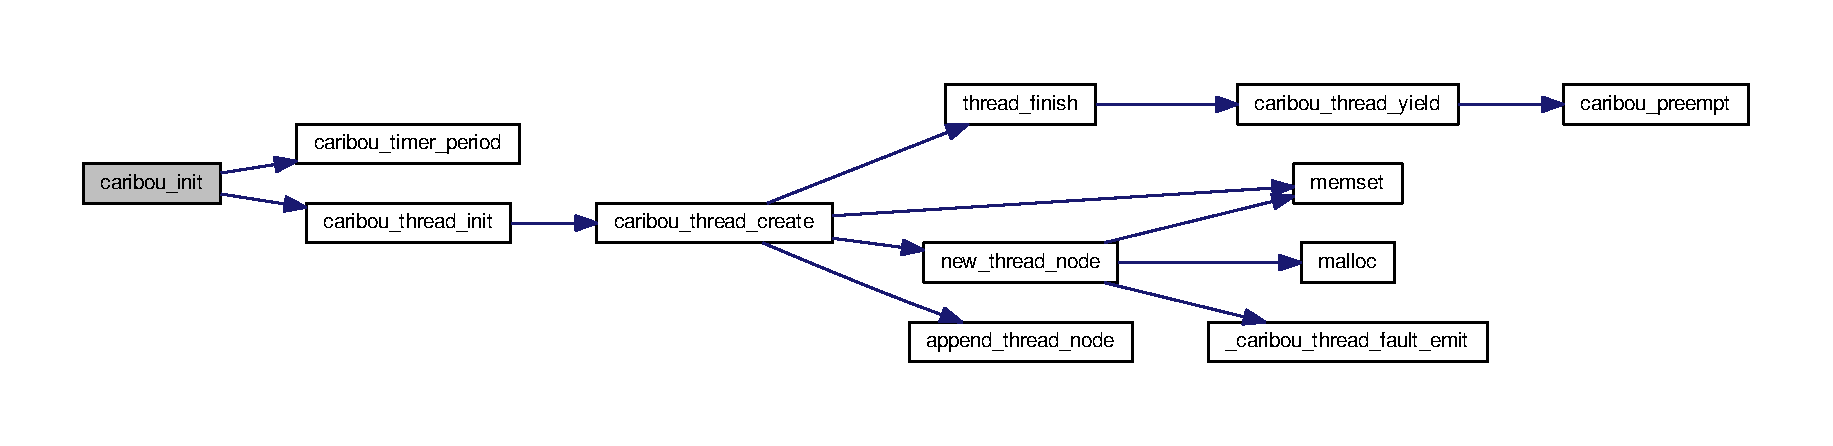
\includegraphics[width=350pt]{caribou_8h_a586f22d1e2495896b4345fa5652e06c9_cgraph}
\end{center}
\end{figure}


\hypertarget{caribou_8h_a2d4f021763a6e4c2918ef9f4285d9585}{\index{caribou.\-h@{caribou.\-h}!caribou\-\_\-init\-\_\-clock@{caribou\-\_\-init\-\_\-clock}}
\index{caribou\-\_\-init\-\_\-clock@{caribou\-\_\-init\-\_\-clock}!caribou.h@{caribou.\-h}}
\subsubsection[{caribou\-\_\-init\-\_\-clock}]{\setlength{\rightskip}{0pt plus 5cm}void caribou\-\_\-init\-\_\-clock (
\begin{DoxyParamCaption}
{}
\end{DoxyParamCaption}
)}}\label{caribou_8h_a2d4f021763a6e4c2918ef9f4285d9585}


Initialize the clock such that jiffies start ticking. 



Definition at line 98 of file caribou.\-c.



Here is the caller graph for this function\-:
\nopagebreak
\begin{figure}[H]
\begin{center}
\leavevmode
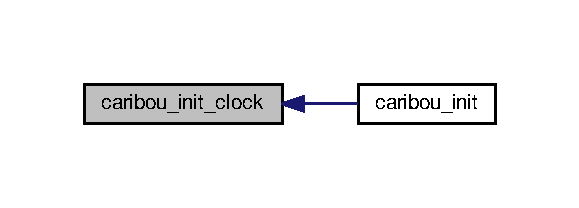
\includegraphics[width=278pt]{caribou_8h_a2d4f021763a6e4c2918ef9f4285d9585_icgraph}
\end{center}
\end{figure}


\hypertarget{caribou_8h_af0bfafa240382bfab4ee9c3279b75b8c}{\index{caribou.\-h@{caribou.\-h}!caribou\-\_\-late\-\_\-init@{caribou\-\_\-late\-\_\-init}}
\index{caribou\-\_\-late\-\_\-init@{caribou\-\_\-late\-\_\-init}!caribou.h@{caribou.\-h}}
\subsubsection[{caribou\-\_\-late\-\_\-init}]{\setlength{\rightskip}{0pt plus 5cm}void caribou\-\_\-late\-\_\-init (
\begin{DoxyParamCaption}
\item[{void}]{}
\end{DoxyParamCaption}
)}}\label{caribou_8h_af0bfafa240382bfab4ee9c3279b75b8c}


A hook to perform late initialization. Static stacks, B\-S\-S, heap, and static contructors are all initialized at this stage. 

\hypertarget{caribou_8h_a3f6b11e983ac91165a6fd14d35aed51f}{\index{caribou.\-h@{caribou.\-h}!caribou\-\_\-lock@{caribou\-\_\-lock}}
\index{caribou\-\_\-lock@{caribou\-\_\-lock}!caribou.h@{caribou.\-h}}
\subsubsection[{caribou\-\_\-lock}]{\setlength{\rightskip}{0pt plus 5cm}int caribou\-\_\-lock (
\begin{DoxyParamCaption}
{}
\end{DoxyParamCaption}
)}}\label{caribou_8h_a3f6b11e983ac91165a6fd14d35aed51f}


Lock the C\-A\-R\-I\-B\-O\-U scheduler onto current thread. 



 

Definition at line 40 of file caribou.\-c.

\hypertarget{caribou_8h_aa8627675e0c04813d45817fda119c5dc}{\index{caribou.\-h@{caribou.\-h}!caribou\-\_\-lock\-\_\-set@{caribou\-\_\-lock\-\_\-set}}
\index{caribou\-\_\-lock\-\_\-set@{caribou\-\_\-lock\-\_\-set}!caribou.h@{caribou.\-h}}
\subsubsection[{caribou\-\_\-lock\-\_\-set}]{\setlength{\rightskip}{0pt plus 5cm}void caribou\-\_\-lock\-\_\-set (
\begin{DoxyParamCaption}
\item[{int}]{state}
\end{DoxyParamCaption}
)}}\label{caribou_8h_aa8627675e0c04813d45817fda119c5dc}


Set the C\-A\-R\-I\-B\-O\-U scheduler lock state. 



 

Definition at line 56 of file caribou.\-c.

\hypertarget{caribou_8h_ae9efd2bf2874e10d63a5cf40bf33802c}{\index{caribou.\-h@{caribou.\-h}!caribou\-\_\-lock\-\_\-state@{caribou\-\_\-lock\-\_\-state}}
\index{caribou\-\_\-lock\-\_\-state@{caribou\-\_\-lock\-\_\-state}!caribou.h@{caribou.\-h}}
\subsubsection[{caribou\-\_\-lock\-\_\-state}]{\setlength{\rightskip}{0pt plus 5cm}int caribou\-\_\-lock\-\_\-state (
\begin{DoxyParamCaption}
{}
\end{DoxyParamCaption}
)}}\label{caribou_8h_ae9efd2bf2874e10d63a5cf40bf33802c}


Test the state of the C\-A\-R\-I\-B\-O\-U scheduler lock. 



 \begin{DoxyReturn}{Returns}
The number of lock state 
\end{DoxyReturn}


Definition at line 32 of file caribou.\-c.

\hypertarget{caribou_8h_a8c39159ad641e81210c3307ab7d64227}{\index{caribou.\-h@{caribou.\-h}!caribou\-\_\-preempt@{caribou\-\_\-preempt}}
\index{caribou\-\_\-preempt@{caribou\-\_\-preempt}!caribou.h@{caribou.\-h}}
\subsubsection[{caribou\-\_\-preempt}]{\setlength{\rightskip}{0pt plus 5cm}void caribou\-\_\-preempt (
\begin{DoxyParamCaption}
{}
\end{DoxyParamCaption}
)}}\label{caribou_8h_a8c39159ad641e81210c3307ab7d64227}


Force scheduler to perform a context switch. 



 

Definition at line 64 of file caribou.\-c.



Here is the caller graph for this function\-:
\nopagebreak
\begin{figure}[H]
\begin{center}
\leavevmode
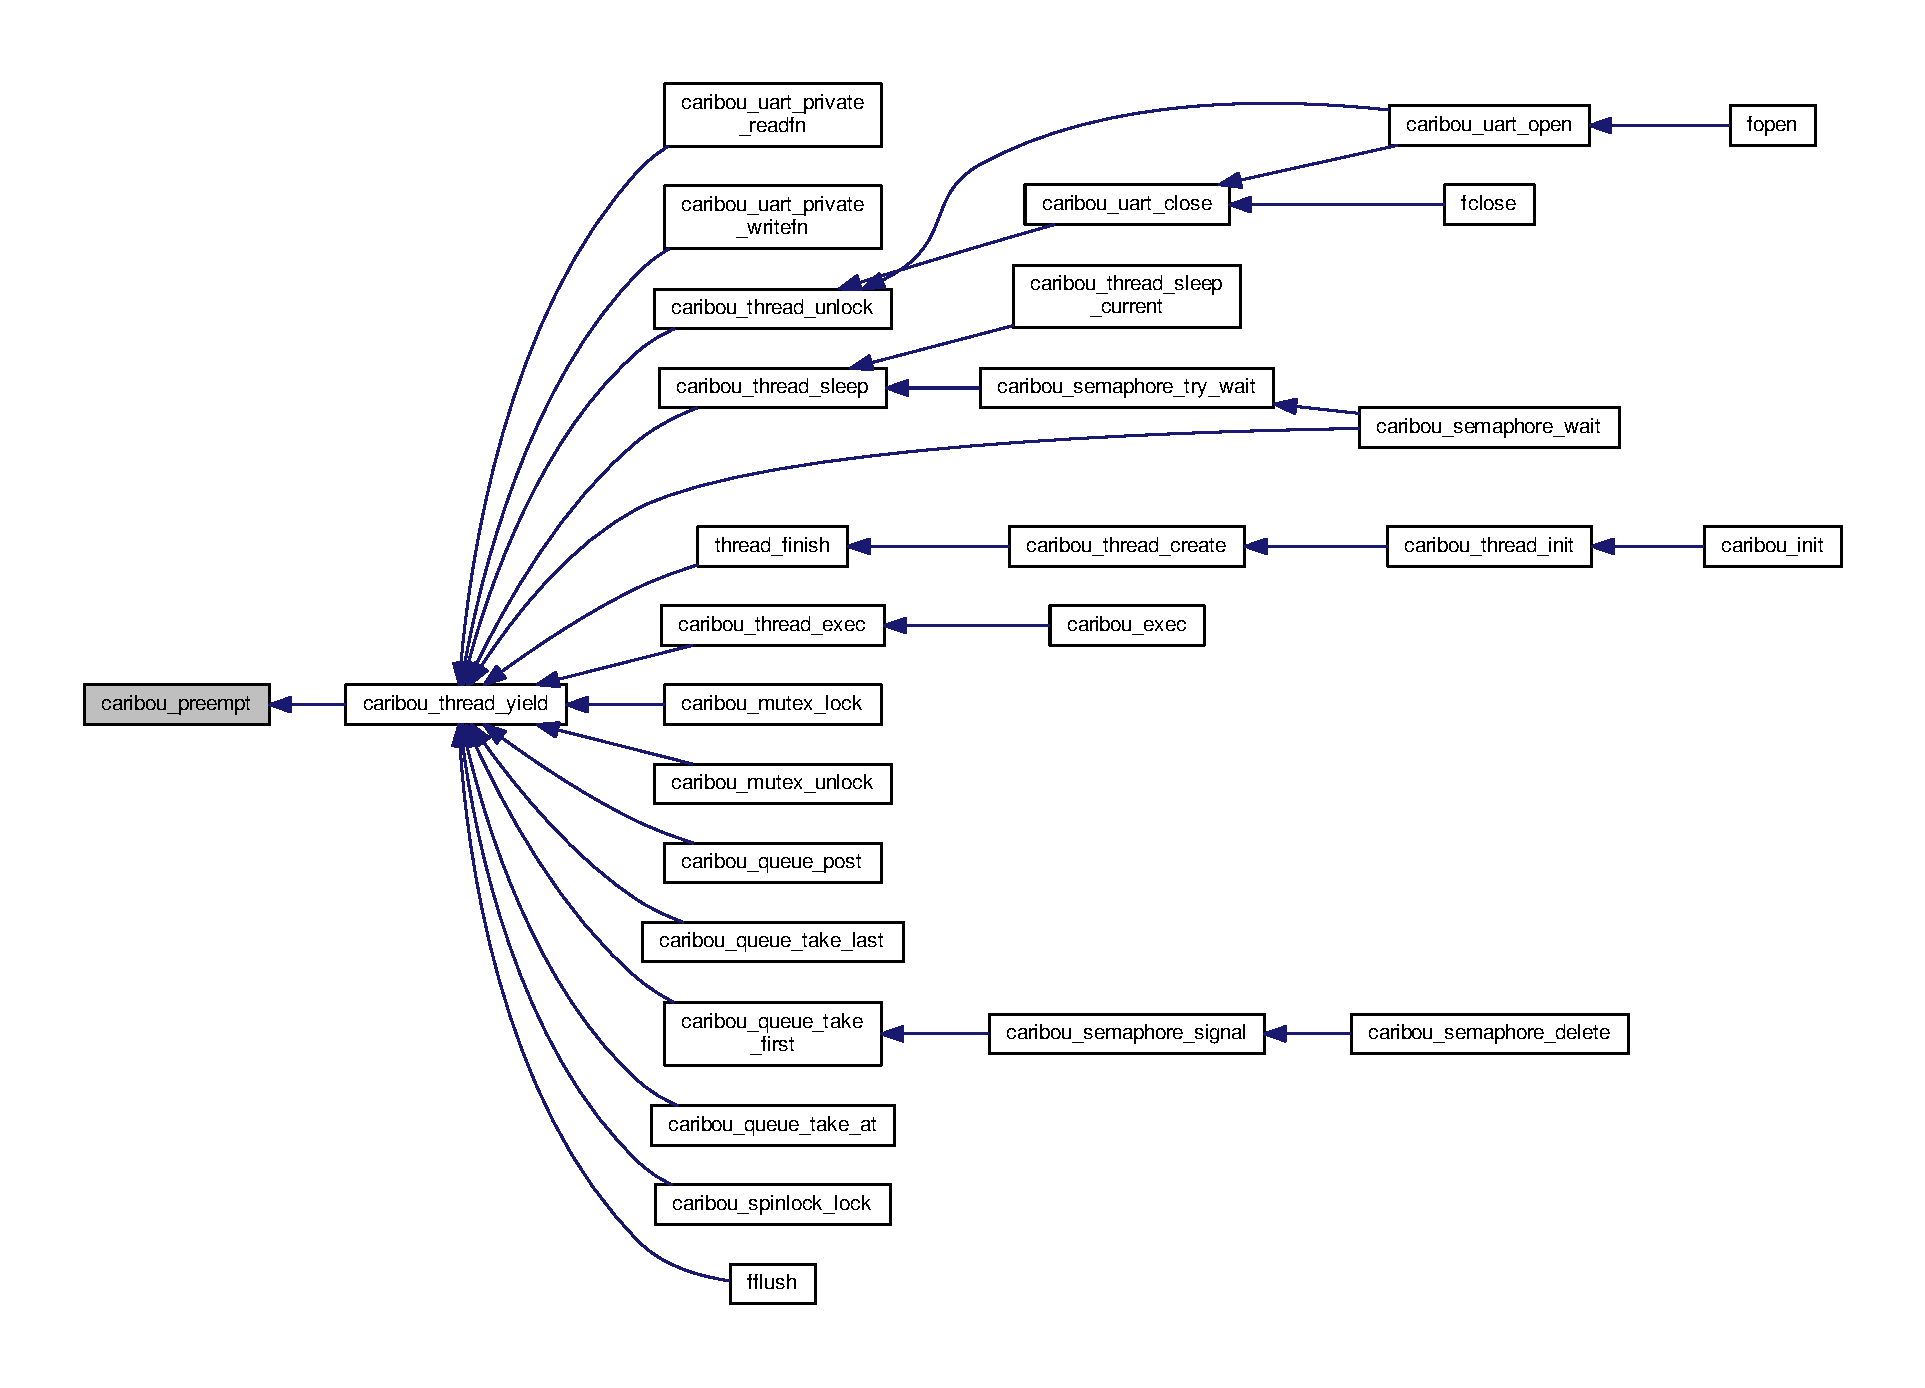
\includegraphics[width=350pt]{caribou_8h_a8c39159ad641e81210c3307ab7d64227_icgraph}
\end{center}
\end{figure}


\hypertarget{caribou_8h_ae6fc3a012fed78adc9a36933057c857f}{\index{caribou.\-h@{caribou.\-h}!caribou\-\_\-unlock@{caribou\-\_\-unlock}}
\index{caribou\-\_\-unlock@{caribou\-\_\-unlock}!caribou.h@{caribou.\-h}}
\subsubsection[{caribou\-\_\-unlock}]{\setlength{\rightskip}{0pt plus 5cm}int caribou\-\_\-unlock (
\begin{DoxyParamCaption}
{}
\end{DoxyParamCaption}
)}}\label{caribou_8h_ae6fc3a012fed78adc9a36933057c857f}


Unlock the C\-A\-R\-I\-B\-O\-U scheduler. 



 

Definition at line 48 of file caribou.\-c.

\hypertarget{caribou_8h_a2eb1e1c5f0f424d820818c92cf3ea0a1}{\index{caribou.\-h@{caribou.\-h}!caribou\-\_\-version@{caribou\-\_\-version}}
\index{caribou\-\_\-version@{caribou\-\_\-version}!caribou.h@{caribou.\-h}}
\subsubsection[{caribou\-\_\-version}]{\setlength{\rightskip}{0pt plus 5cm}const char$\ast$ caribou\-\_\-version (
\begin{DoxyParamCaption}
{}
\end{DoxyParamCaption}
)}}\label{caribou_8h_a2eb1e1c5f0f424d820818c92cf3ea0a1}


 \begin{DoxyReturn}{Returns}
The Caribou Version. 
\end{DoxyReturn}


Definition at line 21 of file caribou.\-c.


\hypertarget{adc_8h}{\section{include/caribou/dev/adc.h File Reference}
\label{adc_8h}\index{include/caribou/dev/adc.\-h@{include/caribou/dev/adc.\-h}}
}
{\ttfamily \#include $<$caribou/kernel/types.\-h$>$}\\*
{\ttfamily \#include $<$chip/adc.\-h$>$}\\*
Include dependency graph for adc.\-h\-:\nopagebreak
\begin{figure}[H]
\begin{center}
\leavevmode
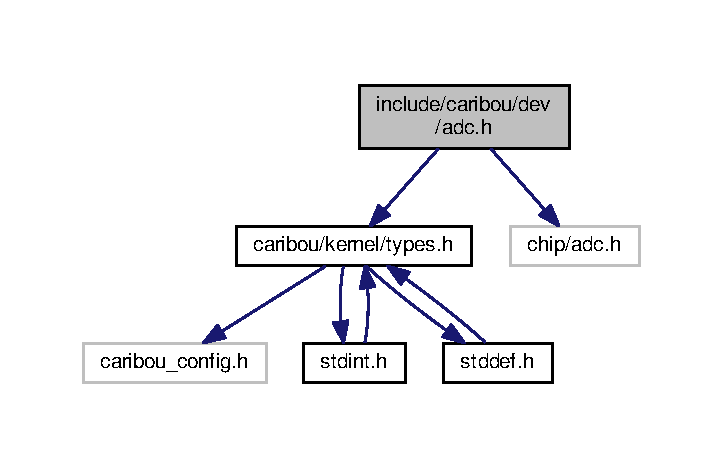
\includegraphics[width=347pt]{adc_8h__incl}
\end{center}
\end{figure}
This graph shows which files directly or indirectly include this file\-:\nopagebreak
\begin{figure}[H]
\begin{center}
\leavevmode
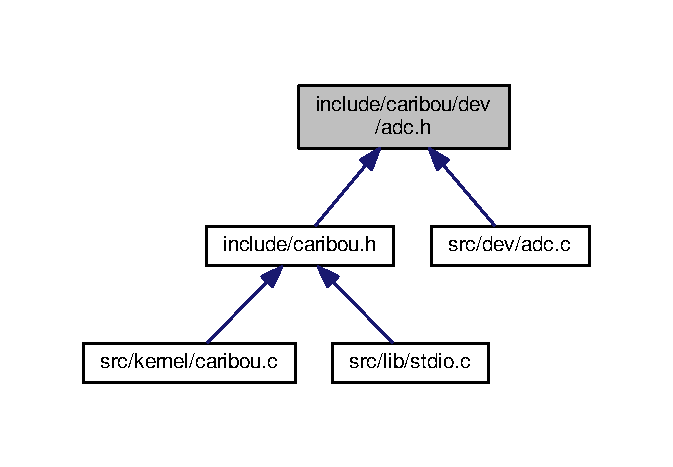
\includegraphics[width=323pt]{adc_8h__dep__incl}
\end{center}
\end{figure}
\subsection*{Data Structures}
\begin{DoxyCompactItemize}
\item 
struct \hyperlink{structcaribou__adc__t}{caribou\-\_\-adc\-\_\-t}
\end{DoxyCompactItemize}
\subsection*{Macros}
\begin{DoxyCompactItemize}
\item 
\#define \hyperlink{adc_8h_a94bc0f69b6be46a97ab75a24a1dde626}{C\-A\-R\-I\-B\-O\-U\-\_\-\-A\-D\-C\-\_\-\-I\-N\-I\-T}(port, channel)~\{port,channel\}
\item 
\#define \hyperlink{adc_8h_a23289bae8c4913b0948093b08a62cb60}{C\-A\-R\-I\-B\-O\-U\-\_\-\-A\-D\-C\-\_\-\-Channel\-\_\-0}~((uint8\-\_\-t)0x00)
\item 
\#define \hyperlink{adc_8h_aa134a8517ec2b40012865fa9fc193549}{C\-A\-R\-I\-B\-O\-U\-\_\-\-A\-D\-C\-\_\-\-Channel\-\_\-1}~((uint8\-\_\-t)0x01)
\item 
\#define \hyperlink{adc_8h_ace3d6ba86c2696520a3a87a5cee7a362}{C\-A\-R\-I\-B\-O\-U\-\_\-\-A\-D\-C\-\_\-\-Channel\-\_\-2}~((uint8\-\_\-t)0x02)
\item 
\#define \hyperlink{adc_8h_a225e31433df02a0b0d3a0154c28baad7}{C\-A\-R\-I\-B\-O\-U\-\_\-\-A\-D\-C\-\_\-\-Channel\-\_\-3}~((uint8\-\_\-t)0x03)
\item 
\#define \hyperlink{adc_8h_a7b30a494dbdf5e8005e32f8b59ca9021}{C\-A\-R\-I\-B\-O\-U\-\_\-\-A\-D\-C\-\_\-\-Channel\-\_\-4}~((uint8\-\_\-t)0x04)
\item 
\#define \hyperlink{adc_8h_aca4b03b7746f40b100f3a3c04c8553d8}{C\-A\-R\-I\-B\-O\-U\-\_\-\-A\-D\-C\-\_\-\-Channel\-\_\-5}~((uint8\-\_\-t)0x05)
\item 
\#define \hyperlink{adc_8h_a4b58443ba4993746ecf65c4bcb7a192f}{C\-A\-R\-I\-B\-O\-U\-\_\-\-A\-D\-C\-\_\-\-Channel\-\_\-6}~((uint8\-\_\-t)0x06)
\item 
\#define \hyperlink{adc_8h_a5eddd2400dfd8cde6b895038daaa47a2}{C\-A\-R\-I\-B\-O\-U\-\_\-\-A\-D\-C\-\_\-\-Channel\-\_\-7}~((uint8\-\_\-t)0x07)
\item 
\#define \hyperlink{adc_8h_ae74f7928d516b4ce391268da1d7cdd91}{C\-A\-R\-I\-B\-O\-U\-\_\-\-A\-D\-C\-\_\-\-Channel\-\_\-8}~((uint8\-\_\-t)0x08)
\item 
\#define \hyperlink{adc_8h_a6493af0066b31d3eb3950f32b178b189}{C\-A\-R\-I\-B\-O\-U\-\_\-\-A\-D\-C\-\_\-\-Channel\-\_\-9}~((uint8\-\_\-t)0x09)
\item 
\#define \hyperlink{adc_8h_a51d41de1a383da9df23ef064f5ee041c}{C\-A\-R\-I\-B\-O\-U\-\_\-\-A\-D\-C\-\_\-\-Channel\-\_\-10}~((uint8\-\_\-t)0x0\-A)
\item 
\#define \hyperlink{adc_8h_adf7a4859e1cbfef6d7e9b47d3ca4c422}{C\-A\-R\-I\-B\-O\-U\-\_\-\-A\-D\-C\-\_\-\-Channel\-\_\-11}~((uint8\-\_\-t)0x0\-B)
\item 
\#define \hyperlink{adc_8h_a5d39430f0889b6166b6af3bfc9e3d87d}{C\-A\-R\-I\-B\-O\-U\-\_\-\-A\-D\-C\-\_\-\-Channel\-\_\-12}~((uint8\-\_\-t)0x0\-C)
\item 
\#define \hyperlink{adc_8h_a91cbea079148956903dd625908142b9c}{C\-A\-R\-I\-B\-O\-U\-\_\-\-A\-D\-C\-\_\-\-Channel\-\_\-13}~((uint8\-\_\-t)0x0\-D)
\item 
\#define \hyperlink{adc_8h_aeb7a4ff29b840c888024c9079e998670}{C\-A\-R\-I\-B\-O\-U\-\_\-\-A\-D\-C\-\_\-\-Channel\-\_\-14}~((uint8\-\_\-t)0x0\-E)
\item 
\#define \hyperlink{adc_8h_ae36ce9557228952741e64a30b93fdd00}{C\-A\-R\-I\-B\-O\-U\-\_\-\-A\-D\-C\-\_\-\-Channel\-\_\-15}~((uint8\-\_\-t)0x0\-F)
\item 
\#define \hyperlink{adc_8h_a9581b87b1aa0aef28f885fc665470110}{C\-A\-R\-I\-B\-O\-U\-\_\-\-A\-D\-C\-\_\-\-Channel\-\_\-16}~((uint8\-\_\-t)0x10)
\item 
\#define \hyperlink{adc_8h_a4f777509d9c116dc7b4d0f2774cf8ec2}{C\-A\-R\-I\-B\-O\-U\-\_\-\-A\-D\-C\-\_\-\-Channel\-\_\-17}~((uint8\-\_\-t)0x11)
\item 
\#define \hyperlink{adc_8h_afa90aa804c4b286808f63c3d415b8264}{C\-A\-R\-I\-B\-O\-U\-\_\-\-A\-D\-C\-\_\-\-Channel\-\_\-18}~((uint8\-\_\-t)0x12)
\item 
\#define \hyperlink{adc_8h_a09aa7d2ec82468968ae85012543ce33c}{C\-A\-R\-I\-B\-O\-U\-\_\-\-A\-D\-C\-\_\-\-Channel\-\_\-19}~((uint8\-\_\-t)0x13)
\item 
\#define \hyperlink{adc_8h_a32e99bcbdd5dbbd40180bac6c9151b15}{C\-A\-R\-I\-B\-O\-U\-\_\-\-A\-D\-C\-\_\-\-Channel\-\_\-20}~((uint8\-\_\-t)0x14)
\item 
\#define \hyperlink{adc_8h_a09524382c423c5d8672176dd381f0a89}{C\-A\-R\-I\-B\-O\-U\-\_\-\-A\-D\-C\-\_\-\-Channel\-\_\-21}~((uint8\-\_\-t)0x15)
\item 
\#define \hyperlink{adc_8h_ac70d54911038ecadab33ad7511aee990}{C\-A\-R\-I\-B\-O\-U\-\_\-\-A\-D\-C\-\_\-\-Channel\-\_\-22}~((uint8\-\_\-t)0x16)
\item 
\#define \hyperlink{adc_8h_a21a19b71176d01fc9a3d98d874245171}{C\-A\-R\-I\-B\-O\-U\-\_\-\-A\-D\-C\-\_\-\-Channel\-\_\-23}~((uint8\-\_\-t)0x17)
\item 
\#define \hyperlink{adc_8h_aadcde700fcb88d66c7d87e55ad2953f1}{C\-A\-R\-I\-B\-O\-U\-\_\-\-A\-D\-C\-\_\-\-Channel\-\_\-24}~((uint8\-\_\-t)0x18)
\item 
\#define \hyperlink{adc_8h_a0a74b7caf78e4886411e63d4659488a0}{C\-A\-R\-I\-B\-O\-U\-\_\-\-A\-D\-C\-\_\-\-Channel\-\_\-25}~((uint8\-\_\-t)0x19)
\item 
\#define \hyperlink{adc_8h_a872d4a36ea129d9928badd79f45bef79}{C\-A\-R\-I\-B\-O\-U\-\_\-\-A\-D\-C\-\_\-\-Channel\-\_\-26}~((uint8\-\_\-t)0x1\-A)
\item 
\#define \hyperlink{adc_8h_a2065271b48a9b3d45d3546a17b5a6548}{C\-A\-R\-I\-B\-O\-U\-\_\-\-A\-D\-C\-\_\-\-Channel\-\_\-27}~((uint8\-\_\-t)0x1\-B)
\item 
\#define \hyperlink{adc_8h_a7741ee36f31e6d41c78bd54c06a84dc2}{C\-A\-R\-I\-B\-O\-U\-\_\-\-A\-D\-C\-\_\-\-Channel\-\_\-28}~((uint8\-\_\-t)0x1\-C)
\item 
\#define \hyperlink{adc_8h_a853ab3e662663606d521be48bf0331ba}{C\-A\-R\-I\-B\-O\-U\-\_\-\-A\-D\-C\-\_\-\-Channel\-\_\-29}~((uint8\-\_\-t)0x1\-D)
\item 
\#define \hyperlink{adc_8h_ac2604b1fff6d8c7f5e2c888e5f5c2733}{C\-A\-R\-I\-B\-O\-U\-\_\-\-A\-D\-C\-\_\-\-Channel\-\_\-30}~((uint8\-\_\-t)0x1\-E)
\item 
\#define \hyperlink{adc_8h_a885c5af367f06d336ead915a3ee69b0a}{C\-A\-R\-I\-B\-O\-U\-\_\-\-A\-D\-C\-\_\-\-Channel\-\_\-31}~((uint8\-\_\-t)0x1\-F)
\end{DoxyCompactItemize}
\subsection*{Functions}
\begin{DoxyCompactItemize}
\item 
int \hyperlink{adc_8h_a8224a5acfc20ae7c16a3b61dd9bfd389}{caribou\-\_\-adc\-\_\-start} (\hyperlink{structcaribou__adc__t}{caribou\-\_\-adc\-\_\-t} $\ast$gpio)
\item 
int \hyperlink{adc_8h_a8ce7be8ab6ba94115f3def188299cd3e}{caribou\-\_\-adc\-\_\-ready} (\hyperlink{structcaribou__adc__t}{caribou\-\_\-adc\-\_\-t} $\ast$gpio)
\item 
chip\-\_\-adc\-\_\-value\-\_\-t \hyperlink{adc_8h_ac8b918555060395b580ce43fcde8ed6f}{caribou\-\_\-adc\-\_\-value} (\hyperlink{structcaribou__adc__t}{caribou\-\_\-adc\-\_\-t} $\ast$gpio)
\end{DoxyCompactItemize}


\subsection{Detailed Description}




\begin{DoxyAuthor}{Author}
Mike Sharkey \href{mailto:mike@pikeaero.com}{\tt mike@pikeaero.\-com}. 
\end{DoxyAuthor}
\begin{DoxyCopyright}{Copyright}
© 2005-\/2013 by Pike Aerospace Research Corporation 

© 2014-\/2015 by Mike Sharkey
\end{DoxyCopyright}
This file is part of C\-A\-R\-I\-B\-O\-U R\-T\-O\-S C\-A\-R\-I\-B\-O\-U R\-T\-O\-S is free software\-: you can redistribute it and/or modify it under the terms of the Beerware License Version 43. \char`\"{}\-T\-H\-E B\-E\-E\-R-\/\-W\-A\-R\-E L\-I\-C\-E\-N\-S\-E\char`\"{} (Revision 43)\-: Mike Sharkey \href{mailto:mike@pikeaero.com}{\tt mike@pikeaero.\-com} wrote this file. As long as you retain this notice you can do whatever you want with this stuff. If we meet some day, and you think this stuff is worth it, you can buy me a beer in return $\sim$ Mike Sharkey 

Definition in file \hyperlink{adc_8h_source}{adc.\-h}.



\subsection{Macro Definition Documentation}
\hypertarget{adc_8h_a23289bae8c4913b0948093b08a62cb60}{\index{adc.\-h@{adc.\-h}!C\-A\-R\-I\-B\-O\-U\-\_\-\-A\-D\-C\-\_\-\-Channel\-\_\-0@{C\-A\-R\-I\-B\-O\-U\-\_\-\-A\-D\-C\-\_\-\-Channel\-\_\-0}}
\index{C\-A\-R\-I\-B\-O\-U\-\_\-\-A\-D\-C\-\_\-\-Channel\-\_\-0@{C\-A\-R\-I\-B\-O\-U\-\_\-\-A\-D\-C\-\_\-\-Channel\-\_\-0}!adc.h@{adc.\-h}}
\subsubsection[{C\-A\-R\-I\-B\-O\-U\-\_\-\-A\-D\-C\-\_\-\-Channel\-\_\-0}]{\setlength{\rightskip}{0pt plus 5cm}\#define C\-A\-R\-I\-B\-O\-U\-\_\-\-A\-D\-C\-\_\-\-Channel\-\_\-0~((uint8\-\_\-t)0x00)}}\label{adc_8h_a23289bae8c4913b0948093b08a62cb60}


Definition at line 34 of file adc.\-h.

\hypertarget{adc_8h_aa134a8517ec2b40012865fa9fc193549}{\index{adc.\-h@{adc.\-h}!C\-A\-R\-I\-B\-O\-U\-\_\-\-A\-D\-C\-\_\-\-Channel\-\_\-1@{C\-A\-R\-I\-B\-O\-U\-\_\-\-A\-D\-C\-\_\-\-Channel\-\_\-1}}
\index{C\-A\-R\-I\-B\-O\-U\-\_\-\-A\-D\-C\-\_\-\-Channel\-\_\-1@{C\-A\-R\-I\-B\-O\-U\-\_\-\-A\-D\-C\-\_\-\-Channel\-\_\-1}!adc.h@{adc.\-h}}
\subsubsection[{C\-A\-R\-I\-B\-O\-U\-\_\-\-A\-D\-C\-\_\-\-Channel\-\_\-1}]{\setlength{\rightskip}{0pt plus 5cm}\#define C\-A\-R\-I\-B\-O\-U\-\_\-\-A\-D\-C\-\_\-\-Channel\-\_\-1~((uint8\-\_\-t)0x01)}}\label{adc_8h_aa134a8517ec2b40012865fa9fc193549}


Definition at line 35 of file adc.\-h.

\hypertarget{adc_8h_a51d41de1a383da9df23ef064f5ee041c}{\index{adc.\-h@{adc.\-h}!C\-A\-R\-I\-B\-O\-U\-\_\-\-A\-D\-C\-\_\-\-Channel\-\_\-10@{C\-A\-R\-I\-B\-O\-U\-\_\-\-A\-D\-C\-\_\-\-Channel\-\_\-10}}
\index{C\-A\-R\-I\-B\-O\-U\-\_\-\-A\-D\-C\-\_\-\-Channel\-\_\-10@{C\-A\-R\-I\-B\-O\-U\-\_\-\-A\-D\-C\-\_\-\-Channel\-\_\-10}!adc.h@{adc.\-h}}
\subsubsection[{C\-A\-R\-I\-B\-O\-U\-\_\-\-A\-D\-C\-\_\-\-Channel\-\_\-10}]{\setlength{\rightskip}{0pt plus 5cm}\#define C\-A\-R\-I\-B\-O\-U\-\_\-\-A\-D\-C\-\_\-\-Channel\-\_\-10~((uint8\-\_\-t)0x0\-A)}}\label{adc_8h_a51d41de1a383da9df23ef064f5ee041c}


Definition at line 44 of file adc.\-h.

\hypertarget{adc_8h_adf7a4859e1cbfef6d7e9b47d3ca4c422}{\index{adc.\-h@{adc.\-h}!C\-A\-R\-I\-B\-O\-U\-\_\-\-A\-D\-C\-\_\-\-Channel\-\_\-11@{C\-A\-R\-I\-B\-O\-U\-\_\-\-A\-D\-C\-\_\-\-Channel\-\_\-11}}
\index{C\-A\-R\-I\-B\-O\-U\-\_\-\-A\-D\-C\-\_\-\-Channel\-\_\-11@{C\-A\-R\-I\-B\-O\-U\-\_\-\-A\-D\-C\-\_\-\-Channel\-\_\-11}!adc.h@{adc.\-h}}
\subsubsection[{C\-A\-R\-I\-B\-O\-U\-\_\-\-A\-D\-C\-\_\-\-Channel\-\_\-11}]{\setlength{\rightskip}{0pt plus 5cm}\#define C\-A\-R\-I\-B\-O\-U\-\_\-\-A\-D\-C\-\_\-\-Channel\-\_\-11~((uint8\-\_\-t)0x0\-B)}}\label{adc_8h_adf7a4859e1cbfef6d7e9b47d3ca4c422}


Definition at line 45 of file adc.\-h.

\hypertarget{adc_8h_a5d39430f0889b6166b6af3bfc9e3d87d}{\index{adc.\-h@{adc.\-h}!C\-A\-R\-I\-B\-O\-U\-\_\-\-A\-D\-C\-\_\-\-Channel\-\_\-12@{C\-A\-R\-I\-B\-O\-U\-\_\-\-A\-D\-C\-\_\-\-Channel\-\_\-12}}
\index{C\-A\-R\-I\-B\-O\-U\-\_\-\-A\-D\-C\-\_\-\-Channel\-\_\-12@{C\-A\-R\-I\-B\-O\-U\-\_\-\-A\-D\-C\-\_\-\-Channel\-\_\-12}!adc.h@{adc.\-h}}
\subsubsection[{C\-A\-R\-I\-B\-O\-U\-\_\-\-A\-D\-C\-\_\-\-Channel\-\_\-12}]{\setlength{\rightskip}{0pt plus 5cm}\#define C\-A\-R\-I\-B\-O\-U\-\_\-\-A\-D\-C\-\_\-\-Channel\-\_\-12~((uint8\-\_\-t)0x0\-C)}}\label{adc_8h_a5d39430f0889b6166b6af3bfc9e3d87d}


Definition at line 46 of file adc.\-h.

\hypertarget{adc_8h_a91cbea079148956903dd625908142b9c}{\index{adc.\-h@{adc.\-h}!C\-A\-R\-I\-B\-O\-U\-\_\-\-A\-D\-C\-\_\-\-Channel\-\_\-13@{C\-A\-R\-I\-B\-O\-U\-\_\-\-A\-D\-C\-\_\-\-Channel\-\_\-13}}
\index{C\-A\-R\-I\-B\-O\-U\-\_\-\-A\-D\-C\-\_\-\-Channel\-\_\-13@{C\-A\-R\-I\-B\-O\-U\-\_\-\-A\-D\-C\-\_\-\-Channel\-\_\-13}!adc.h@{adc.\-h}}
\subsubsection[{C\-A\-R\-I\-B\-O\-U\-\_\-\-A\-D\-C\-\_\-\-Channel\-\_\-13}]{\setlength{\rightskip}{0pt plus 5cm}\#define C\-A\-R\-I\-B\-O\-U\-\_\-\-A\-D\-C\-\_\-\-Channel\-\_\-13~((uint8\-\_\-t)0x0\-D)}}\label{adc_8h_a91cbea079148956903dd625908142b9c}


Definition at line 47 of file adc.\-h.

\hypertarget{adc_8h_aeb7a4ff29b840c888024c9079e998670}{\index{adc.\-h@{adc.\-h}!C\-A\-R\-I\-B\-O\-U\-\_\-\-A\-D\-C\-\_\-\-Channel\-\_\-14@{C\-A\-R\-I\-B\-O\-U\-\_\-\-A\-D\-C\-\_\-\-Channel\-\_\-14}}
\index{C\-A\-R\-I\-B\-O\-U\-\_\-\-A\-D\-C\-\_\-\-Channel\-\_\-14@{C\-A\-R\-I\-B\-O\-U\-\_\-\-A\-D\-C\-\_\-\-Channel\-\_\-14}!adc.h@{adc.\-h}}
\subsubsection[{C\-A\-R\-I\-B\-O\-U\-\_\-\-A\-D\-C\-\_\-\-Channel\-\_\-14}]{\setlength{\rightskip}{0pt plus 5cm}\#define C\-A\-R\-I\-B\-O\-U\-\_\-\-A\-D\-C\-\_\-\-Channel\-\_\-14~((uint8\-\_\-t)0x0\-E)}}\label{adc_8h_aeb7a4ff29b840c888024c9079e998670}


Definition at line 48 of file adc.\-h.

\hypertarget{adc_8h_ae36ce9557228952741e64a30b93fdd00}{\index{adc.\-h@{adc.\-h}!C\-A\-R\-I\-B\-O\-U\-\_\-\-A\-D\-C\-\_\-\-Channel\-\_\-15@{C\-A\-R\-I\-B\-O\-U\-\_\-\-A\-D\-C\-\_\-\-Channel\-\_\-15}}
\index{C\-A\-R\-I\-B\-O\-U\-\_\-\-A\-D\-C\-\_\-\-Channel\-\_\-15@{C\-A\-R\-I\-B\-O\-U\-\_\-\-A\-D\-C\-\_\-\-Channel\-\_\-15}!adc.h@{adc.\-h}}
\subsubsection[{C\-A\-R\-I\-B\-O\-U\-\_\-\-A\-D\-C\-\_\-\-Channel\-\_\-15}]{\setlength{\rightskip}{0pt plus 5cm}\#define C\-A\-R\-I\-B\-O\-U\-\_\-\-A\-D\-C\-\_\-\-Channel\-\_\-15~((uint8\-\_\-t)0x0\-F)}}\label{adc_8h_ae36ce9557228952741e64a30b93fdd00}


Definition at line 49 of file adc.\-h.

\hypertarget{adc_8h_a9581b87b1aa0aef28f885fc665470110}{\index{adc.\-h@{adc.\-h}!C\-A\-R\-I\-B\-O\-U\-\_\-\-A\-D\-C\-\_\-\-Channel\-\_\-16@{C\-A\-R\-I\-B\-O\-U\-\_\-\-A\-D\-C\-\_\-\-Channel\-\_\-16}}
\index{C\-A\-R\-I\-B\-O\-U\-\_\-\-A\-D\-C\-\_\-\-Channel\-\_\-16@{C\-A\-R\-I\-B\-O\-U\-\_\-\-A\-D\-C\-\_\-\-Channel\-\_\-16}!adc.h@{adc.\-h}}
\subsubsection[{C\-A\-R\-I\-B\-O\-U\-\_\-\-A\-D\-C\-\_\-\-Channel\-\_\-16}]{\setlength{\rightskip}{0pt plus 5cm}\#define C\-A\-R\-I\-B\-O\-U\-\_\-\-A\-D\-C\-\_\-\-Channel\-\_\-16~((uint8\-\_\-t)0x10)}}\label{adc_8h_a9581b87b1aa0aef28f885fc665470110}


Definition at line 50 of file adc.\-h.

\hypertarget{adc_8h_a4f777509d9c116dc7b4d0f2774cf8ec2}{\index{adc.\-h@{adc.\-h}!C\-A\-R\-I\-B\-O\-U\-\_\-\-A\-D\-C\-\_\-\-Channel\-\_\-17@{C\-A\-R\-I\-B\-O\-U\-\_\-\-A\-D\-C\-\_\-\-Channel\-\_\-17}}
\index{C\-A\-R\-I\-B\-O\-U\-\_\-\-A\-D\-C\-\_\-\-Channel\-\_\-17@{C\-A\-R\-I\-B\-O\-U\-\_\-\-A\-D\-C\-\_\-\-Channel\-\_\-17}!adc.h@{adc.\-h}}
\subsubsection[{C\-A\-R\-I\-B\-O\-U\-\_\-\-A\-D\-C\-\_\-\-Channel\-\_\-17}]{\setlength{\rightskip}{0pt plus 5cm}\#define C\-A\-R\-I\-B\-O\-U\-\_\-\-A\-D\-C\-\_\-\-Channel\-\_\-17~((uint8\-\_\-t)0x11)}}\label{adc_8h_a4f777509d9c116dc7b4d0f2774cf8ec2}


Definition at line 51 of file adc.\-h.

\hypertarget{adc_8h_afa90aa804c4b286808f63c3d415b8264}{\index{adc.\-h@{adc.\-h}!C\-A\-R\-I\-B\-O\-U\-\_\-\-A\-D\-C\-\_\-\-Channel\-\_\-18@{C\-A\-R\-I\-B\-O\-U\-\_\-\-A\-D\-C\-\_\-\-Channel\-\_\-18}}
\index{C\-A\-R\-I\-B\-O\-U\-\_\-\-A\-D\-C\-\_\-\-Channel\-\_\-18@{C\-A\-R\-I\-B\-O\-U\-\_\-\-A\-D\-C\-\_\-\-Channel\-\_\-18}!adc.h@{adc.\-h}}
\subsubsection[{C\-A\-R\-I\-B\-O\-U\-\_\-\-A\-D\-C\-\_\-\-Channel\-\_\-18}]{\setlength{\rightskip}{0pt plus 5cm}\#define C\-A\-R\-I\-B\-O\-U\-\_\-\-A\-D\-C\-\_\-\-Channel\-\_\-18~((uint8\-\_\-t)0x12)}}\label{adc_8h_afa90aa804c4b286808f63c3d415b8264}


Definition at line 52 of file adc.\-h.

\hypertarget{adc_8h_a09aa7d2ec82468968ae85012543ce33c}{\index{adc.\-h@{adc.\-h}!C\-A\-R\-I\-B\-O\-U\-\_\-\-A\-D\-C\-\_\-\-Channel\-\_\-19@{C\-A\-R\-I\-B\-O\-U\-\_\-\-A\-D\-C\-\_\-\-Channel\-\_\-19}}
\index{C\-A\-R\-I\-B\-O\-U\-\_\-\-A\-D\-C\-\_\-\-Channel\-\_\-19@{C\-A\-R\-I\-B\-O\-U\-\_\-\-A\-D\-C\-\_\-\-Channel\-\_\-19}!adc.h@{adc.\-h}}
\subsubsection[{C\-A\-R\-I\-B\-O\-U\-\_\-\-A\-D\-C\-\_\-\-Channel\-\_\-19}]{\setlength{\rightskip}{0pt plus 5cm}\#define C\-A\-R\-I\-B\-O\-U\-\_\-\-A\-D\-C\-\_\-\-Channel\-\_\-19~((uint8\-\_\-t)0x13)}}\label{adc_8h_a09aa7d2ec82468968ae85012543ce33c}


Definition at line 53 of file adc.\-h.

\hypertarget{adc_8h_ace3d6ba86c2696520a3a87a5cee7a362}{\index{adc.\-h@{adc.\-h}!C\-A\-R\-I\-B\-O\-U\-\_\-\-A\-D\-C\-\_\-\-Channel\-\_\-2@{C\-A\-R\-I\-B\-O\-U\-\_\-\-A\-D\-C\-\_\-\-Channel\-\_\-2}}
\index{C\-A\-R\-I\-B\-O\-U\-\_\-\-A\-D\-C\-\_\-\-Channel\-\_\-2@{C\-A\-R\-I\-B\-O\-U\-\_\-\-A\-D\-C\-\_\-\-Channel\-\_\-2}!adc.h@{adc.\-h}}
\subsubsection[{C\-A\-R\-I\-B\-O\-U\-\_\-\-A\-D\-C\-\_\-\-Channel\-\_\-2}]{\setlength{\rightskip}{0pt plus 5cm}\#define C\-A\-R\-I\-B\-O\-U\-\_\-\-A\-D\-C\-\_\-\-Channel\-\_\-2~((uint8\-\_\-t)0x02)}}\label{adc_8h_ace3d6ba86c2696520a3a87a5cee7a362}


Definition at line 36 of file adc.\-h.

\hypertarget{adc_8h_a32e99bcbdd5dbbd40180bac6c9151b15}{\index{adc.\-h@{adc.\-h}!C\-A\-R\-I\-B\-O\-U\-\_\-\-A\-D\-C\-\_\-\-Channel\-\_\-20@{C\-A\-R\-I\-B\-O\-U\-\_\-\-A\-D\-C\-\_\-\-Channel\-\_\-20}}
\index{C\-A\-R\-I\-B\-O\-U\-\_\-\-A\-D\-C\-\_\-\-Channel\-\_\-20@{C\-A\-R\-I\-B\-O\-U\-\_\-\-A\-D\-C\-\_\-\-Channel\-\_\-20}!adc.h@{adc.\-h}}
\subsubsection[{C\-A\-R\-I\-B\-O\-U\-\_\-\-A\-D\-C\-\_\-\-Channel\-\_\-20}]{\setlength{\rightskip}{0pt plus 5cm}\#define C\-A\-R\-I\-B\-O\-U\-\_\-\-A\-D\-C\-\_\-\-Channel\-\_\-20~((uint8\-\_\-t)0x14)}}\label{adc_8h_a32e99bcbdd5dbbd40180bac6c9151b15}


Definition at line 54 of file adc.\-h.

\hypertarget{adc_8h_a09524382c423c5d8672176dd381f0a89}{\index{adc.\-h@{adc.\-h}!C\-A\-R\-I\-B\-O\-U\-\_\-\-A\-D\-C\-\_\-\-Channel\-\_\-21@{C\-A\-R\-I\-B\-O\-U\-\_\-\-A\-D\-C\-\_\-\-Channel\-\_\-21}}
\index{C\-A\-R\-I\-B\-O\-U\-\_\-\-A\-D\-C\-\_\-\-Channel\-\_\-21@{C\-A\-R\-I\-B\-O\-U\-\_\-\-A\-D\-C\-\_\-\-Channel\-\_\-21}!adc.h@{adc.\-h}}
\subsubsection[{C\-A\-R\-I\-B\-O\-U\-\_\-\-A\-D\-C\-\_\-\-Channel\-\_\-21}]{\setlength{\rightskip}{0pt plus 5cm}\#define C\-A\-R\-I\-B\-O\-U\-\_\-\-A\-D\-C\-\_\-\-Channel\-\_\-21~((uint8\-\_\-t)0x15)}}\label{adc_8h_a09524382c423c5d8672176dd381f0a89}


Definition at line 55 of file adc.\-h.

\hypertarget{adc_8h_ac70d54911038ecadab33ad7511aee990}{\index{adc.\-h@{adc.\-h}!C\-A\-R\-I\-B\-O\-U\-\_\-\-A\-D\-C\-\_\-\-Channel\-\_\-22@{C\-A\-R\-I\-B\-O\-U\-\_\-\-A\-D\-C\-\_\-\-Channel\-\_\-22}}
\index{C\-A\-R\-I\-B\-O\-U\-\_\-\-A\-D\-C\-\_\-\-Channel\-\_\-22@{C\-A\-R\-I\-B\-O\-U\-\_\-\-A\-D\-C\-\_\-\-Channel\-\_\-22}!adc.h@{adc.\-h}}
\subsubsection[{C\-A\-R\-I\-B\-O\-U\-\_\-\-A\-D\-C\-\_\-\-Channel\-\_\-22}]{\setlength{\rightskip}{0pt plus 5cm}\#define C\-A\-R\-I\-B\-O\-U\-\_\-\-A\-D\-C\-\_\-\-Channel\-\_\-22~((uint8\-\_\-t)0x16)}}\label{adc_8h_ac70d54911038ecadab33ad7511aee990}


Definition at line 56 of file adc.\-h.

\hypertarget{adc_8h_a21a19b71176d01fc9a3d98d874245171}{\index{adc.\-h@{adc.\-h}!C\-A\-R\-I\-B\-O\-U\-\_\-\-A\-D\-C\-\_\-\-Channel\-\_\-23@{C\-A\-R\-I\-B\-O\-U\-\_\-\-A\-D\-C\-\_\-\-Channel\-\_\-23}}
\index{C\-A\-R\-I\-B\-O\-U\-\_\-\-A\-D\-C\-\_\-\-Channel\-\_\-23@{C\-A\-R\-I\-B\-O\-U\-\_\-\-A\-D\-C\-\_\-\-Channel\-\_\-23}!adc.h@{adc.\-h}}
\subsubsection[{C\-A\-R\-I\-B\-O\-U\-\_\-\-A\-D\-C\-\_\-\-Channel\-\_\-23}]{\setlength{\rightskip}{0pt plus 5cm}\#define C\-A\-R\-I\-B\-O\-U\-\_\-\-A\-D\-C\-\_\-\-Channel\-\_\-23~((uint8\-\_\-t)0x17)}}\label{adc_8h_a21a19b71176d01fc9a3d98d874245171}


Definition at line 57 of file adc.\-h.

\hypertarget{adc_8h_aadcde700fcb88d66c7d87e55ad2953f1}{\index{adc.\-h@{adc.\-h}!C\-A\-R\-I\-B\-O\-U\-\_\-\-A\-D\-C\-\_\-\-Channel\-\_\-24@{C\-A\-R\-I\-B\-O\-U\-\_\-\-A\-D\-C\-\_\-\-Channel\-\_\-24}}
\index{C\-A\-R\-I\-B\-O\-U\-\_\-\-A\-D\-C\-\_\-\-Channel\-\_\-24@{C\-A\-R\-I\-B\-O\-U\-\_\-\-A\-D\-C\-\_\-\-Channel\-\_\-24}!adc.h@{adc.\-h}}
\subsubsection[{C\-A\-R\-I\-B\-O\-U\-\_\-\-A\-D\-C\-\_\-\-Channel\-\_\-24}]{\setlength{\rightskip}{0pt plus 5cm}\#define C\-A\-R\-I\-B\-O\-U\-\_\-\-A\-D\-C\-\_\-\-Channel\-\_\-24~((uint8\-\_\-t)0x18)}}\label{adc_8h_aadcde700fcb88d66c7d87e55ad2953f1}


Definition at line 58 of file adc.\-h.

\hypertarget{adc_8h_a0a74b7caf78e4886411e63d4659488a0}{\index{adc.\-h@{adc.\-h}!C\-A\-R\-I\-B\-O\-U\-\_\-\-A\-D\-C\-\_\-\-Channel\-\_\-25@{C\-A\-R\-I\-B\-O\-U\-\_\-\-A\-D\-C\-\_\-\-Channel\-\_\-25}}
\index{C\-A\-R\-I\-B\-O\-U\-\_\-\-A\-D\-C\-\_\-\-Channel\-\_\-25@{C\-A\-R\-I\-B\-O\-U\-\_\-\-A\-D\-C\-\_\-\-Channel\-\_\-25}!adc.h@{adc.\-h}}
\subsubsection[{C\-A\-R\-I\-B\-O\-U\-\_\-\-A\-D\-C\-\_\-\-Channel\-\_\-25}]{\setlength{\rightskip}{0pt plus 5cm}\#define C\-A\-R\-I\-B\-O\-U\-\_\-\-A\-D\-C\-\_\-\-Channel\-\_\-25~((uint8\-\_\-t)0x19)}}\label{adc_8h_a0a74b7caf78e4886411e63d4659488a0}


Definition at line 59 of file adc.\-h.

\hypertarget{adc_8h_a872d4a36ea129d9928badd79f45bef79}{\index{adc.\-h@{adc.\-h}!C\-A\-R\-I\-B\-O\-U\-\_\-\-A\-D\-C\-\_\-\-Channel\-\_\-26@{C\-A\-R\-I\-B\-O\-U\-\_\-\-A\-D\-C\-\_\-\-Channel\-\_\-26}}
\index{C\-A\-R\-I\-B\-O\-U\-\_\-\-A\-D\-C\-\_\-\-Channel\-\_\-26@{C\-A\-R\-I\-B\-O\-U\-\_\-\-A\-D\-C\-\_\-\-Channel\-\_\-26}!adc.h@{adc.\-h}}
\subsubsection[{C\-A\-R\-I\-B\-O\-U\-\_\-\-A\-D\-C\-\_\-\-Channel\-\_\-26}]{\setlength{\rightskip}{0pt plus 5cm}\#define C\-A\-R\-I\-B\-O\-U\-\_\-\-A\-D\-C\-\_\-\-Channel\-\_\-26~((uint8\-\_\-t)0x1\-A)}}\label{adc_8h_a872d4a36ea129d9928badd79f45bef79}


Definition at line 60 of file adc.\-h.

\hypertarget{adc_8h_a2065271b48a9b3d45d3546a17b5a6548}{\index{adc.\-h@{adc.\-h}!C\-A\-R\-I\-B\-O\-U\-\_\-\-A\-D\-C\-\_\-\-Channel\-\_\-27@{C\-A\-R\-I\-B\-O\-U\-\_\-\-A\-D\-C\-\_\-\-Channel\-\_\-27}}
\index{C\-A\-R\-I\-B\-O\-U\-\_\-\-A\-D\-C\-\_\-\-Channel\-\_\-27@{C\-A\-R\-I\-B\-O\-U\-\_\-\-A\-D\-C\-\_\-\-Channel\-\_\-27}!adc.h@{adc.\-h}}
\subsubsection[{C\-A\-R\-I\-B\-O\-U\-\_\-\-A\-D\-C\-\_\-\-Channel\-\_\-27}]{\setlength{\rightskip}{0pt plus 5cm}\#define C\-A\-R\-I\-B\-O\-U\-\_\-\-A\-D\-C\-\_\-\-Channel\-\_\-27~((uint8\-\_\-t)0x1\-B)}}\label{adc_8h_a2065271b48a9b3d45d3546a17b5a6548}


Definition at line 61 of file adc.\-h.

\hypertarget{adc_8h_a7741ee36f31e6d41c78bd54c06a84dc2}{\index{adc.\-h@{adc.\-h}!C\-A\-R\-I\-B\-O\-U\-\_\-\-A\-D\-C\-\_\-\-Channel\-\_\-28@{C\-A\-R\-I\-B\-O\-U\-\_\-\-A\-D\-C\-\_\-\-Channel\-\_\-28}}
\index{C\-A\-R\-I\-B\-O\-U\-\_\-\-A\-D\-C\-\_\-\-Channel\-\_\-28@{C\-A\-R\-I\-B\-O\-U\-\_\-\-A\-D\-C\-\_\-\-Channel\-\_\-28}!adc.h@{adc.\-h}}
\subsubsection[{C\-A\-R\-I\-B\-O\-U\-\_\-\-A\-D\-C\-\_\-\-Channel\-\_\-28}]{\setlength{\rightskip}{0pt plus 5cm}\#define C\-A\-R\-I\-B\-O\-U\-\_\-\-A\-D\-C\-\_\-\-Channel\-\_\-28~((uint8\-\_\-t)0x1\-C)}}\label{adc_8h_a7741ee36f31e6d41c78bd54c06a84dc2}


Definition at line 62 of file adc.\-h.

\hypertarget{adc_8h_a853ab3e662663606d521be48bf0331ba}{\index{adc.\-h@{adc.\-h}!C\-A\-R\-I\-B\-O\-U\-\_\-\-A\-D\-C\-\_\-\-Channel\-\_\-29@{C\-A\-R\-I\-B\-O\-U\-\_\-\-A\-D\-C\-\_\-\-Channel\-\_\-29}}
\index{C\-A\-R\-I\-B\-O\-U\-\_\-\-A\-D\-C\-\_\-\-Channel\-\_\-29@{C\-A\-R\-I\-B\-O\-U\-\_\-\-A\-D\-C\-\_\-\-Channel\-\_\-29}!adc.h@{adc.\-h}}
\subsubsection[{C\-A\-R\-I\-B\-O\-U\-\_\-\-A\-D\-C\-\_\-\-Channel\-\_\-29}]{\setlength{\rightskip}{0pt plus 5cm}\#define C\-A\-R\-I\-B\-O\-U\-\_\-\-A\-D\-C\-\_\-\-Channel\-\_\-29~((uint8\-\_\-t)0x1\-D)}}\label{adc_8h_a853ab3e662663606d521be48bf0331ba}


Definition at line 63 of file adc.\-h.

\hypertarget{adc_8h_a225e31433df02a0b0d3a0154c28baad7}{\index{adc.\-h@{adc.\-h}!C\-A\-R\-I\-B\-O\-U\-\_\-\-A\-D\-C\-\_\-\-Channel\-\_\-3@{C\-A\-R\-I\-B\-O\-U\-\_\-\-A\-D\-C\-\_\-\-Channel\-\_\-3}}
\index{C\-A\-R\-I\-B\-O\-U\-\_\-\-A\-D\-C\-\_\-\-Channel\-\_\-3@{C\-A\-R\-I\-B\-O\-U\-\_\-\-A\-D\-C\-\_\-\-Channel\-\_\-3}!adc.h@{adc.\-h}}
\subsubsection[{C\-A\-R\-I\-B\-O\-U\-\_\-\-A\-D\-C\-\_\-\-Channel\-\_\-3}]{\setlength{\rightskip}{0pt plus 5cm}\#define C\-A\-R\-I\-B\-O\-U\-\_\-\-A\-D\-C\-\_\-\-Channel\-\_\-3~((uint8\-\_\-t)0x03)}}\label{adc_8h_a225e31433df02a0b0d3a0154c28baad7}


Definition at line 37 of file adc.\-h.

\hypertarget{adc_8h_ac2604b1fff6d8c7f5e2c888e5f5c2733}{\index{adc.\-h@{adc.\-h}!C\-A\-R\-I\-B\-O\-U\-\_\-\-A\-D\-C\-\_\-\-Channel\-\_\-30@{C\-A\-R\-I\-B\-O\-U\-\_\-\-A\-D\-C\-\_\-\-Channel\-\_\-30}}
\index{C\-A\-R\-I\-B\-O\-U\-\_\-\-A\-D\-C\-\_\-\-Channel\-\_\-30@{C\-A\-R\-I\-B\-O\-U\-\_\-\-A\-D\-C\-\_\-\-Channel\-\_\-30}!adc.h@{adc.\-h}}
\subsubsection[{C\-A\-R\-I\-B\-O\-U\-\_\-\-A\-D\-C\-\_\-\-Channel\-\_\-30}]{\setlength{\rightskip}{0pt plus 5cm}\#define C\-A\-R\-I\-B\-O\-U\-\_\-\-A\-D\-C\-\_\-\-Channel\-\_\-30~((uint8\-\_\-t)0x1\-E)}}\label{adc_8h_ac2604b1fff6d8c7f5e2c888e5f5c2733}


Definition at line 64 of file adc.\-h.

\hypertarget{adc_8h_a885c5af367f06d336ead915a3ee69b0a}{\index{adc.\-h@{adc.\-h}!C\-A\-R\-I\-B\-O\-U\-\_\-\-A\-D\-C\-\_\-\-Channel\-\_\-31@{C\-A\-R\-I\-B\-O\-U\-\_\-\-A\-D\-C\-\_\-\-Channel\-\_\-31}}
\index{C\-A\-R\-I\-B\-O\-U\-\_\-\-A\-D\-C\-\_\-\-Channel\-\_\-31@{C\-A\-R\-I\-B\-O\-U\-\_\-\-A\-D\-C\-\_\-\-Channel\-\_\-31}!adc.h@{adc.\-h}}
\subsubsection[{C\-A\-R\-I\-B\-O\-U\-\_\-\-A\-D\-C\-\_\-\-Channel\-\_\-31}]{\setlength{\rightskip}{0pt plus 5cm}\#define C\-A\-R\-I\-B\-O\-U\-\_\-\-A\-D\-C\-\_\-\-Channel\-\_\-31~((uint8\-\_\-t)0x1\-F)}}\label{adc_8h_a885c5af367f06d336ead915a3ee69b0a}


Definition at line 65 of file adc.\-h.

\hypertarget{adc_8h_a7b30a494dbdf5e8005e32f8b59ca9021}{\index{adc.\-h@{adc.\-h}!C\-A\-R\-I\-B\-O\-U\-\_\-\-A\-D\-C\-\_\-\-Channel\-\_\-4@{C\-A\-R\-I\-B\-O\-U\-\_\-\-A\-D\-C\-\_\-\-Channel\-\_\-4}}
\index{C\-A\-R\-I\-B\-O\-U\-\_\-\-A\-D\-C\-\_\-\-Channel\-\_\-4@{C\-A\-R\-I\-B\-O\-U\-\_\-\-A\-D\-C\-\_\-\-Channel\-\_\-4}!adc.h@{adc.\-h}}
\subsubsection[{C\-A\-R\-I\-B\-O\-U\-\_\-\-A\-D\-C\-\_\-\-Channel\-\_\-4}]{\setlength{\rightskip}{0pt plus 5cm}\#define C\-A\-R\-I\-B\-O\-U\-\_\-\-A\-D\-C\-\_\-\-Channel\-\_\-4~((uint8\-\_\-t)0x04)}}\label{adc_8h_a7b30a494dbdf5e8005e32f8b59ca9021}


Definition at line 38 of file adc.\-h.

\hypertarget{adc_8h_aca4b03b7746f40b100f3a3c04c8553d8}{\index{adc.\-h@{adc.\-h}!C\-A\-R\-I\-B\-O\-U\-\_\-\-A\-D\-C\-\_\-\-Channel\-\_\-5@{C\-A\-R\-I\-B\-O\-U\-\_\-\-A\-D\-C\-\_\-\-Channel\-\_\-5}}
\index{C\-A\-R\-I\-B\-O\-U\-\_\-\-A\-D\-C\-\_\-\-Channel\-\_\-5@{C\-A\-R\-I\-B\-O\-U\-\_\-\-A\-D\-C\-\_\-\-Channel\-\_\-5}!adc.h@{adc.\-h}}
\subsubsection[{C\-A\-R\-I\-B\-O\-U\-\_\-\-A\-D\-C\-\_\-\-Channel\-\_\-5}]{\setlength{\rightskip}{0pt plus 5cm}\#define C\-A\-R\-I\-B\-O\-U\-\_\-\-A\-D\-C\-\_\-\-Channel\-\_\-5~((uint8\-\_\-t)0x05)}}\label{adc_8h_aca4b03b7746f40b100f3a3c04c8553d8}


Definition at line 39 of file adc.\-h.

\hypertarget{adc_8h_a4b58443ba4993746ecf65c4bcb7a192f}{\index{adc.\-h@{adc.\-h}!C\-A\-R\-I\-B\-O\-U\-\_\-\-A\-D\-C\-\_\-\-Channel\-\_\-6@{C\-A\-R\-I\-B\-O\-U\-\_\-\-A\-D\-C\-\_\-\-Channel\-\_\-6}}
\index{C\-A\-R\-I\-B\-O\-U\-\_\-\-A\-D\-C\-\_\-\-Channel\-\_\-6@{C\-A\-R\-I\-B\-O\-U\-\_\-\-A\-D\-C\-\_\-\-Channel\-\_\-6}!adc.h@{adc.\-h}}
\subsubsection[{C\-A\-R\-I\-B\-O\-U\-\_\-\-A\-D\-C\-\_\-\-Channel\-\_\-6}]{\setlength{\rightskip}{0pt plus 5cm}\#define C\-A\-R\-I\-B\-O\-U\-\_\-\-A\-D\-C\-\_\-\-Channel\-\_\-6~((uint8\-\_\-t)0x06)}}\label{adc_8h_a4b58443ba4993746ecf65c4bcb7a192f}


Definition at line 40 of file adc.\-h.

\hypertarget{adc_8h_a5eddd2400dfd8cde6b895038daaa47a2}{\index{adc.\-h@{adc.\-h}!C\-A\-R\-I\-B\-O\-U\-\_\-\-A\-D\-C\-\_\-\-Channel\-\_\-7@{C\-A\-R\-I\-B\-O\-U\-\_\-\-A\-D\-C\-\_\-\-Channel\-\_\-7}}
\index{C\-A\-R\-I\-B\-O\-U\-\_\-\-A\-D\-C\-\_\-\-Channel\-\_\-7@{C\-A\-R\-I\-B\-O\-U\-\_\-\-A\-D\-C\-\_\-\-Channel\-\_\-7}!adc.h@{adc.\-h}}
\subsubsection[{C\-A\-R\-I\-B\-O\-U\-\_\-\-A\-D\-C\-\_\-\-Channel\-\_\-7}]{\setlength{\rightskip}{0pt plus 5cm}\#define C\-A\-R\-I\-B\-O\-U\-\_\-\-A\-D\-C\-\_\-\-Channel\-\_\-7~((uint8\-\_\-t)0x07)}}\label{adc_8h_a5eddd2400dfd8cde6b895038daaa47a2}


Definition at line 41 of file adc.\-h.

\hypertarget{adc_8h_ae74f7928d516b4ce391268da1d7cdd91}{\index{adc.\-h@{adc.\-h}!C\-A\-R\-I\-B\-O\-U\-\_\-\-A\-D\-C\-\_\-\-Channel\-\_\-8@{C\-A\-R\-I\-B\-O\-U\-\_\-\-A\-D\-C\-\_\-\-Channel\-\_\-8}}
\index{C\-A\-R\-I\-B\-O\-U\-\_\-\-A\-D\-C\-\_\-\-Channel\-\_\-8@{C\-A\-R\-I\-B\-O\-U\-\_\-\-A\-D\-C\-\_\-\-Channel\-\_\-8}!adc.h@{adc.\-h}}
\subsubsection[{C\-A\-R\-I\-B\-O\-U\-\_\-\-A\-D\-C\-\_\-\-Channel\-\_\-8}]{\setlength{\rightskip}{0pt plus 5cm}\#define C\-A\-R\-I\-B\-O\-U\-\_\-\-A\-D\-C\-\_\-\-Channel\-\_\-8~((uint8\-\_\-t)0x08)}}\label{adc_8h_ae74f7928d516b4ce391268da1d7cdd91}


Definition at line 42 of file adc.\-h.

\hypertarget{adc_8h_a6493af0066b31d3eb3950f32b178b189}{\index{adc.\-h@{adc.\-h}!C\-A\-R\-I\-B\-O\-U\-\_\-\-A\-D\-C\-\_\-\-Channel\-\_\-9@{C\-A\-R\-I\-B\-O\-U\-\_\-\-A\-D\-C\-\_\-\-Channel\-\_\-9}}
\index{C\-A\-R\-I\-B\-O\-U\-\_\-\-A\-D\-C\-\_\-\-Channel\-\_\-9@{C\-A\-R\-I\-B\-O\-U\-\_\-\-A\-D\-C\-\_\-\-Channel\-\_\-9}!adc.h@{adc.\-h}}
\subsubsection[{C\-A\-R\-I\-B\-O\-U\-\_\-\-A\-D\-C\-\_\-\-Channel\-\_\-9}]{\setlength{\rightskip}{0pt plus 5cm}\#define C\-A\-R\-I\-B\-O\-U\-\_\-\-A\-D\-C\-\_\-\-Channel\-\_\-9~((uint8\-\_\-t)0x09)}}\label{adc_8h_a6493af0066b31d3eb3950f32b178b189}


Definition at line 43 of file adc.\-h.

\hypertarget{adc_8h_a94bc0f69b6be46a97ab75a24a1dde626}{\index{adc.\-h@{adc.\-h}!C\-A\-R\-I\-B\-O\-U\-\_\-\-A\-D\-C\-\_\-\-I\-N\-I\-T@{C\-A\-R\-I\-B\-O\-U\-\_\-\-A\-D\-C\-\_\-\-I\-N\-I\-T}}
\index{C\-A\-R\-I\-B\-O\-U\-\_\-\-A\-D\-C\-\_\-\-I\-N\-I\-T@{C\-A\-R\-I\-B\-O\-U\-\_\-\-A\-D\-C\-\_\-\-I\-N\-I\-T}!adc.h@{adc.\-h}}
\subsubsection[{C\-A\-R\-I\-B\-O\-U\-\_\-\-A\-D\-C\-\_\-\-I\-N\-I\-T}]{\setlength{\rightskip}{0pt plus 5cm}\#define C\-A\-R\-I\-B\-O\-U\-\_\-\-A\-D\-C\-\_\-\-I\-N\-I\-T(
\begin{DoxyParamCaption}
\item[{}]{port, }
\item[{}]{channel}
\end{DoxyParamCaption}
)~\{port,channel\}}}\label{adc_8h_a94bc0f69b6be46a97ab75a24a1dde626}


Definition at line 32 of file adc.\-h.



\subsection{Function Documentation}
\hypertarget{adc_8h_a8ce7be8ab6ba94115f3def188299cd3e}{\index{adc.\-h@{adc.\-h}!caribou\-\_\-adc\-\_\-ready@{caribou\-\_\-adc\-\_\-ready}}
\index{caribou\-\_\-adc\-\_\-ready@{caribou\-\_\-adc\-\_\-ready}!adc.h@{adc.\-h}}
\subsubsection[{caribou\-\_\-adc\-\_\-ready}]{\setlength{\rightskip}{0pt plus 5cm}int caribou\-\_\-adc\-\_\-ready (
\begin{DoxyParamCaption}
\item[{{\bf caribou\-\_\-adc\-\_\-t} $\ast$}]{gpio}
\end{DoxyParamCaption}
)}}\label{adc_8h_a8ce7be8ab6ba94115f3def188299cd3e}


Definition at line 22 of file adc.\-c.

\hypertarget{adc_8h_a8224a5acfc20ae7c16a3b61dd9bfd389}{\index{adc.\-h@{adc.\-h}!caribou\-\_\-adc\-\_\-start@{caribou\-\_\-adc\-\_\-start}}
\index{caribou\-\_\-adc\-\_\-start@{caribou\-\_\-adc\-\_\-start}!adc.h@{adc.\-h}}
\subsubsection[{caribou\-\_\-adc\-\_\-start}]{\setlength{\rightskip}{0pt plus 5cm}int caribou\-\_\-adc\-\_\-start (
\begin{DoxyParamCaption}
\item[{{\bf caribou\-\_\-adc\-\_\-t} $\ast$}]{gpio}
\end{DoxyParamCaption}
)}}\label{adc_8h_a8224a5acfc20ae7c16a3b61dd9bfd389}


Definition at line 17 of file adc.\-c.

\hypertarget{adc_8h_ac8b918555060395b580ce43fcde8ed6f}{\index{adc.\-h@{adc.\-h}!caribou\-\_\-adc\-\_\-value@{caribou\-\_\-adc\-\_\-value}}
\index{caribou\-\_\-adc\-\_\-value@{caribou\-\_\-adc\-\_\-value}!adc.h@{adc.\-h}}
\subsubsection[{caribou\-\_\-adc\-\_\-value}]{\setlength{\rightskip}{0pt plus 5cm}chip\-\_\-adc\-\_\-value\-\_\-t caribou\-\_\-adc\-\_\-value (
\begin{DoxyParamCaption}
\item[{{\bf caribou\-\_\-adc\-\_\-t} $\ast$}]{gpio}
\end{DoxyParamCaption}
)}}\label{adc_8h_ac8b918555060395b580ce43fcde8ed6f}


Definition at line 27 of file adc.\-c.


\hypertarget{gpio_8h}{\section{include/caribou/dev/gpio.h File Reference}
\label{gpio_8h}\index{include/caribou/dev/gpio.\-h@{include/caribou/dev/gpio.\-h}}
}
{\ttfamily \#include $<$caribou/kernel/types.\-h$>$}\\*
{\ttfamily \#include $<$chip/gpio.\-h$>$}\\*
Include dependency graph for gpio.\-h\-:
\nopagebreak
\begin{figure}[H]
\begin{center}
\leavevmode
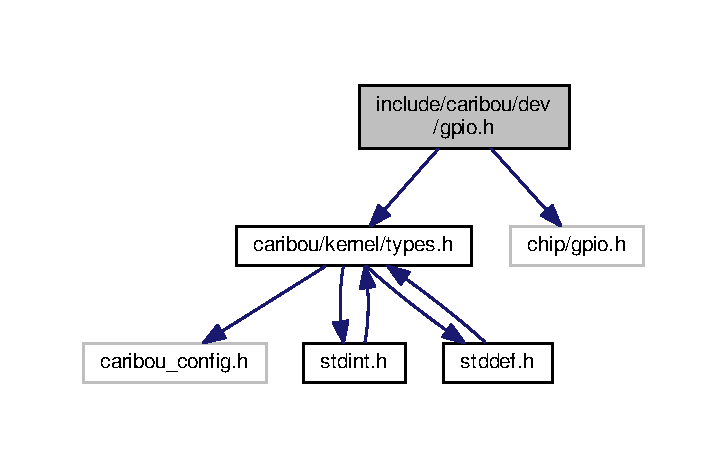
\includegraphics[width=349pt]{gpio_8h__incl}
\end{center}
\end{figure}
This graph shows which files directly or indirectly include this file\-:
\nopagebreak
\begin{figure}[H]
\begin{center}
\leavevmode
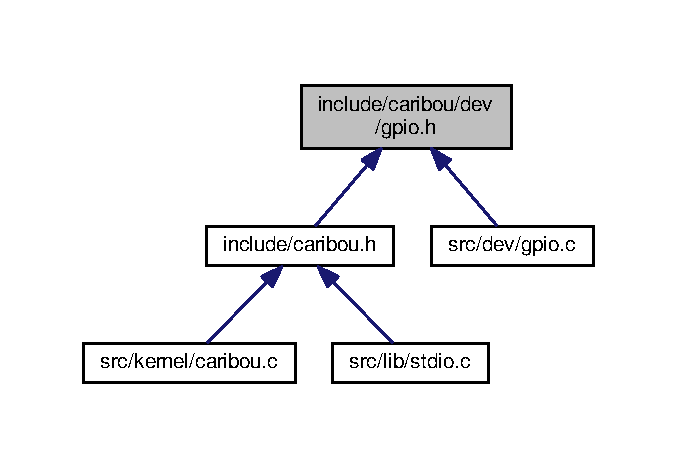
\includegraphics[width=325pt]{gpio_8h__dep__incl}
\end{center}
\end{figure}
\subsection*{Data Structures}
\begin{DoxyCompactItemize}
\item 
struct \hyperlink{structcaribou__gpio__t}{caribou\-\_\-gpio\-\_\-t}
\end{DoxyCompactItemize}
\subsection*{Macros}
\begin{DoxyCompactItemize}
\item 
\#define \hyperlink{gpio_8h_a81205bf9142cd9955e4e3e02b1719288}{C\-A\-R\-I\-B\-O\-U\-\_\-\-G\-P\-I\-O\-\_\-\-I\-N\-I\-T}(port, pinmask)~\{port,pinmask\}
\item 
\#define \hyperlink{gpio_8h_ad1a6f9e2b79ddceb0d3b7bf58df33ab6}{C\-A\-R\-I\-B\-O\-U\-\_\-\-G\-P\-I\-O\-\_\-\-P\-I\-N\-\_\-0}~(1$<$$<$0)
\item 
\#define \hyperlink{gpio_8h_aaa345cfee2350e67e64439e8bff747cb}{C\-A\-R\-I\-B\-O\-U\-\_\-\-G\-P\-I\-O\-\_\-\-P\-I\-N\-\_\-1}~(1$<$$<$1)
\item 
\#define \hyperlink{gpio_8h_a85963cf2bf8b880acc623e3e3abe8694}{C\-A\-R\-I\-B\-O\-U\-\_\-\-G\-P\-I\-O\-\_\-\-P\-I\-N\-\_\-2}~(1$<$$<$2)
\item 
\#define \hyperlink{gpio_8h_aa9f542bfb47bc3f4135c94918c93df49}{C\-A\-R\-I\-B\-O\-U\-\_\-\-G\-P\-I\-O\-\_\-\-P\-I\-N\-\_\-3}~(1$<$$<$3)
\item 
\#define \hyperlink{gpio_8h_a1fa6e7cf838ef5722b79d2f7f9945daf}{C\-A\-R\-I\-B\-O\-U\-\_\-\-G\-P\-I\-O\-\_\-\-P\-I\-N\-\_\-4}~(1$<$$<$4)
\item 
\#define \hyperlink{gpio_8h_a21329aefd750c07707e48f9db8b90846}{C\-A\-R\-I\-B\-O\-U\-\_\-\-G\-P\-I\-O\-\_\-\-P\-I\-N\-\_\-5}~(1$<$$<$5)
\item 
\#define \hyperlink{gpio_8h_adce602370438a2b3a2e7f373fb826ba3}{C\-A\-R\-I\-B\-O\-U\-\_\-\-G\-P\-I\-O\-\_\-\-P\-I\-N\-\_\-6}~(1$<$$<$6)
\item 
\#define \hyperlink{gpio_8h_a86bf2efe483758639beb576246ac8142}{C\-A\-R\-I\-B\-O\-U\-\_\-\-G\-P\-I\-O\-\_\-\-P\-I\-N\-\_\-7}~(1$<$$<$7)
\item 
\#define \hyperlink{gpio_8h_a204f2032e95d5cf5164adbecafdeab22}{C\-A\-R\-I\-B\-O\-U\-\_\-\-G\-P\-I\-O\-\_\-\-P\-I\-N\-\_\-8}~(1$<$$<$8)
\item 
\#define \hyperlink{gpio_8h_ae25a870938bbb69fdfe571ba457a8d53}{C\-A\-R\-I\-B\-O\-U\-\_\-\-G\-P\-I\-O\-\_\-\-P\-I\-N\-\_\-9}~(1$<$$<$9)
\item 
\#define \hyperlink{gpio_8h_adab24c51bc6ea2d8a034313031a48f7c}{C\-A\-R\-I\-B\-O\-U\-\_\-\-G\-P\-I\-O\-\_\-\-P\-I\-N\-\_\-10}~(1$<$$<$10)
\item 
\#define \hyperlink{gpio_8h_abd09dc00df08645daf0416603cd8c97b}{C\-A\-R\-I\-B\-O\-U\-\_\-\-G\-P\-I\-O\-\_\-\-P\-I\-N\-\_\-11}~(1$<$$<$11)
\item 
\#define \hyperlink{gpio_8h_a80d3c31e223c62c9032a153001b24886}{C\-A\-R\-I\-B\-O\-U\-\_\-\-G\-P\-I\-O\-\_\-\-P\-I\-N\-\_\-12}~(1$<$$<$12)
\item 
\#define \hyperlink{gpio_8h_a1f675dd1e5b8a8129d4556c1cd0293d5}{C\-A\-R\-I\-B\-O\-U\-\_\-\-G\-P\-I\-O\-\_\-\-P\-I\-N\-\_\-13}~(1$<$$<$13)
\item 
\#define \hyperlink{gpio_8h_a4f1454ee7c6614237f6233dfc2c4ae22}{C\-A\-R\-I\-B\-O\-U\-\_\-\-G\-P\-I\-O\-\_\-\-P\-I\-N\-\_\-14}~(1$<$$<$14)
\item 
\#define \hyperlink{gpio_8h_a036a87986ebf8280fa1c4a170b235d99}{C\-A\-R\-I\-B\-O\-U\-\_\-\-G\-P\-I\-O\-\_\-\-P\-I\-N\-\_\-15}~(1$<$$<$15)
\item 
\#define \hyperlink{gpio_8h_aff1fc762caf78e50d39d4a5e6c0a968e}{C\-A\-R\-I\-B\-O\-U\-\_\-\-G\-P\-I\-O\-\_\-\-P\-I\-N\-\_\-16}~(1$<$$<$16)
\item 
\#define \hyperlink{gpio_8h_ae715c3f03b87b1c96794ae41a72a0254}{C\-A\-R\-I\-B\-O\-U\-\_\-\-G\-P\-I\-O\-\_\-\-P\-I\-N\-\_\-17}~(1$<$$<$17)
\item 
\#define \hyperlink{gpio_8h_a3e01020b5a7f9c313d82debe634f2009}{C\-A\-R\-I\-B\-O\-U\-\_\-\-G\-P\-I\-O\-\_\-\-P\-I\-N\-\_\-18}~(1$<$$<$18)
\item 
\#define \hyperlink{gpio_8h_adf9be064223b858b92ffbdb13bd9bb94}{C\-A\-R\-I\-B\-O\-U\-\_\-\-G\-P\-I\-O\-\_\-\-P\-I\-N\-\_\-19}~(1$<$$<$19)
\item 
\#define \hyperlink{gpio_8h_ab653fff4366370d92ad0afff109c9518}{C\-A\-R\-I\-B\-O\-U\-\_\-\-G\-P\-I\-O\-\_\-\-P\-I\-N\-\_\-20}~(1$<$$<$20)
\item 
\#define \hyperlink{gpio_8h_a109664fee1dacb8095c3073e48642e6b}{C\-A\-R\-I\-B\-O\-U\-\_\-\-G\-P\-I\-O\-\_\-\-P\-I\-N\-\_\-21}~(1$<$$<$21)
\item 
\#define \hyperlink{gpio_8h_a57ff48e119e5df82a3cbb7653d73f39a}{C\-A\-R\-I\-B\-O\-U\-\_\-\-G\-P\-I\-O\-\_\-\-P\-I\-N\-\_\-22}~(1$<$$<$22)
\item 
\#define \hyperlink{gpio_8h_aea3e11069680b985bdd6d19344e69f56}{C\-A\-R\-I\-B\-O\-U\-\_\-\-G\-P\-I\-O\-\_\-\-P\-I\-N\-\_\-23}~(1$<$$<$23)
\item 
\#define \hyperlink{gpio_8h_a7b23993f1a4f6595075b8bb5b4bb9a2a}{C\-A\-R\-I\-B\-O\-U\-\_\-\-G\-P\-I\-O\-\_\-\-P\-I\-N\-\_\-24}~(1$<$$<$24)
\item 
\#define \hyperlink{gpio_8h_a08541bbf3cbf2d0590f6878f98c5fafe}{C\-A\-R\-I\-B\-O\-U\-\_\-\-G\-P\-I\-O\-\_\-\-P\-I\-N\-\_\-25}~(1$<$$<$25)
\item 
\#define \hyperlink{gpio_8h_a6266a262744f70766b35dc54019acc18}{C\-A\-R\-I\-B\-O\-U\-\_\-\-G\-P\-I\-O\-\_\-\-P\-I\-N\-\_\-26}~(1$<$$<$26)
\item 
\#define \hyperlink{gpio_8h_a76c95839a5171c991f97dbb40b50398f}{C\-A\-R\-I\-B\-O\-U\-\_\-\-G\-P\-I\-O\-\_\-\-P\-I\-N\-\_\-27}~(1$<$$<$27)
\item 
\#define \hyperlink{gpio_8h_acc9651f59d3f9c5b6f00099cd2cef61e}{C\-A\-R\-I\-B\-O\-U\-\_\-\-G\-P\-I\-O\-\_\-\-P\-I\-N\-\_\-28}~(1$<$$<$28)
\item 
\#define \hyperlink{gpio_8h_aa49a7b612ef12d7593ccd3283e36c3e8}{C\-A\-R\-I\-B\-O\-U\-\_\-\-G\-P\-I\-O\-\_\-\-P\-I\-N\-\_\-29}~(1$<$$<$29)
\item 
\#define \hyperlink{gpio_8h_ab1570342948b69d9e9ba71ca51cd1fbf}{C\-A\-R\-I\-B\-O\-U\-\_\-\-G\-P\-I\-O\-\_\-\-P\-I\-N\-\_\-30}~(1$<$$<$30)
\item 
\#define \hyperlink{gpio_8h_a92ba6576f3a52a003466ab4f17ec535e}{C\-A\-R\-I\-B\-O\-U\-\_\-\-G\-P\-I\-O\-\_\-\-P\-I\-N\-\_\-31}~(1$<$$<$31)
\item 
\#define \hyperlink{gpio_8h_a9bfb187f104d8baada074cf98e19a490}{caribou\-\_\-gpio\-\_\-set\-\_\-output}(gpio)~chip\-\_\-gpio\-\_\-set\-\_\-output((gpio)-\/$>$port,(gpio)-\/$>$pinmask)
\item 
\#define \hyperlink{gpio_8h_a2195f9d13d0405be84597e3e854891b8}{caribou\-\_\-gpio\-\_\-set\-\_\-input}(gpio)~chip\-\_\-gpio\-\_\-set\-\_\-input((gpio)-\/$>$port,(gpio)-\/$>$pinmask)
\item 
\#define \hyperlink{gpio_8h_a88a9d0c91683277e5c9c24f00d0081ea}{caribou\-\_\-gpio\-\_\-set\-\_\-pullup}(gpio)~chip\-\_\-gpio\-\_\-set\-\_\-pullup((gpio)-\/$>$port,(gpio)-\/$>$pinmask)
\item 
\#define \hyperlink{gpio_8h_a08747a61214148c83cd465e78b520b76}{caribou\-\_\-gpio\-\_\-set\-\_\-pulldown}(gpio)~chip\-\_\-gpio\-\_\-set\-\_\-pulldown((gpio)-\/$>$port,(gpio)-\/$>$pinmask)
\item 
\#define \hyperlink{gpio_8h_aac1d060cdfc0858a63941aadaae56e1e}{caribou\-\_\-gpio\-\_\-toggle}(gpio)~chip\-\_\-gpio\-\_\-toggle((gpio)-\/$>$port,(gpio)-\/$>$pinmask)
\item 
\#define \hyperlink{gpio_8h_ada242efca3020303e6d1013f14834e46}{caribou\-\_\-gpio\-\_\-set}(gpio)~chip\-\_\-gpio\-\_\-set((gpio)-\/$>$port,(gpio)-\/$>$pinmask)
\item 
\#define \hyperlink{gpio_8h_ad20de6fc6a359380043ad94e5cd69f50}{caribou\-\_\-gpio\-\_\-reset}(gpio)~chip\-\_\-gpio\-\_\-reset((gpio)-\/$>$port,(gpio)-\/$>$pinmask)
\item 
\#define \hyperlink{gpio_8h_a1a8c9abf6fd9ea13d6615be3611e3573}{caribou\-\_\-gpio\-\_\-pinstate}(gpio)~chip\-\_\-gpio\-\_\-pinstate((gpio)-\/$>$port,(gpio)-\/$>$pinmask)
\item 
\#define \hyperlink{gpio_8h_a913a8e70279db2746c55bdf54f3d0dd1}{caribou\-\_\-gpio\-\_\-pinmask}(gpio)~((gpio)-\/$>$pinmask)
\item 
\#define \hyperlink{gpio_8h_aaa8b61c2396d91f5b2a7f8b7e725a326}{caribou\-\_\-gpio\-\_\-write}(gpio, state)~\{if(state) \hyperlink{gpio_8h_ada242efca3020303e6d1013f14834e46}{caribou\-\_\-gpio\-\_\-set}(gpio); else \hyperlink{gpio_8h_ad20de6fc6a359380043ad94e5cd69f50}{caribou\-\_\-gpio\-\_\-reset}(gpio);\}
\end{DoxyCompactItemize}


\subsection{Macro Definition Documentation}
\hypertarget{gpio_8h_a81205bf9142cd9955e4e3e02b1719288}{\index{gpio.\-h@{gpio.\-h}!C\-A\-R\-I\-B\-O\-U\-\_\-\-G\-P\-I\-O\-\_\-\-I\-N\-I\-T@{C\-A\-R\-I\-B\-O\-U\-\_\-\-G\-P\-I\-O\-\_\-\-I\-N\-I\-T}}
\index{C\-A\-R\-I\-B\-O\-U\-\_\-\-G\-P\-I\-O\-\_\-\-I\-N\-I\-T@{C\-A\-R\-I\-B\-O\-U\-\_\-\-G\-P\-I\-O\-\_\-\-I\-N\-I\-T}!gpio.h@{gpio.\-h}}
\subsubsection[{C\-A\-R\-I\-B\-O\-U\-\_\-\-G\-P\-I\-O\-\_\-\-I\-N\-I\-T}]{\setlength{\rightskip}{0pt plus 5cm}\#define C\-A\-R\-I\-B\-O\-U\-\_\-\-G\-P\-I\-O\-\_\-\-I\-N\-I\-T(
\begin{DoxyParamCaption}
\item[{}]{port, }
\item[{}]{pinmask}
\end{DoxyParamCaption}
)~\{port,pinmask\}}}\label{gpio_8h_a81205bf9142cd9955e4e3e02b1719288}


Definition at line 42 of file gpio.\-h.

\hypertarget{gpio_8h_ad1a6f9e2b79ddceb0d3b7bf58df33ab6}{\index{gpio.\-h@{gpio.\-h}!C\-A\-R\-I\-B\-O\-U\-\_\-\-G\-P\-I\-O\-\_\-\-P\-I\-N\-\_\-0@{C\-A\-R\-I\-B\-O\-U\-\_\-\-G\-P\-I\-O\-\_\-\-P\-I\-N\-\_\-0}}
\index{C\-A\-R\-I\-B\-O\-U\-\_\-\-G\-P\-I\-O\-\_\-\-P\-I\-N\-\_\-0@{C\-A\-R\-I\-B\-O\-U\-\_\-\-G\-P\-I\-O\-\_\-\-P\-I\-N\-\_\-0}!gpio.h@{gpio.\-h}}
\subsubsection[{C\-A\-R\-I\-B\-O\-U\-\_\-\-G\-P\-I\-O\-\_\-\-P\-I\-N\-\_\-0}]{\setlength{\rightskip}{0pt plus 5cm}\#define C\-A\-R\-I\-B\-O\-U\-\_\-\-G\-P\-I\-O\-\_\-\-P\-I\-N\-\_\-0~(1$<$$<$0)}}\label{gpio_8h_ad1a6f9e2b79ddceb0d3b7bf58df33ab6}


Definition at line 44 of file gpio.\-h.

\hypertarget{gpio_8h_aaa345cfee2350e67e64439e8bff747cb}{\index{gpio.\-h@{gpio.\-h}!C\-A\-R\-I\-B\-O\-U\-\_\-\-G\-P\-I\-O\-\_\-\-P\-I\-N\-\_\-1@{C\-A\-R\-I\-B\-O\-U\-\_\-\-G\-P\-I\-O\-\_\-\-P\-I\-N\-\_\-1}}
\index{C\-A\-R\-I\-B\-O\-U\-\_\-\-G\-P\-I\-O\-\_\-\-P\-I\-N\-\_\-1@{C\-A\-R\-I\-B\-O\-U\-\_\-\-G\-P\-I\-O\-\_\-\-P\-I\-N\-\_\-1}!gpio.h@{gpio.\-h}}
\subsubsection[{C\-A\-R\-I\-B\-O\-U\-\_\-\-G\-P\-I\-O\-\_\-\-P\-I\-N\-\_\-1}]{\setlength{\rightskip}{0pt plus 5cm}\#define C\-A\-R\-I\-B\-O\-U\-\_\-\-G\-P\-I\-O\-\_\-\-P\-I\-N\-\_\-1~(1$<$$<$1)}}\label{gpio_8h_aaa345cfee2350e67e64439e8bff747cb}


Definition at line 45 of file gpio.\-h.

\hypertarget{gpio_8h_adab24c51bc6ea2d8a034313031a48f7c}{\index{gpio.\-h@{gpio.\-h}!C\-A\-R\-I\-B\-O\-U\-\_\-\-G\-P\-I\-O\-\_\-\-P\-I\-N\-\_\-10@{C\-A\-R\-I\-B\-O\-U\-\_\-\-G\-P\-I\-O\-\_\-\-P\-I\-N\-\_\-10}}
\index{C\-A\-R\-I\-B\-O\-U\-\_\-\-G\-P\-I\-O\-\_\-\-P\-I\-N\-\_\-10@{C\-A\-R\-I\-B\-O\-U\-\_\-\-G\-P\-I\-O\-\_\-\-P\-I\-N\-\_\-10}!gpio.h@{gpio.\-h}}
\subsubsection[{C\-A\-R\-I\-B\-O\-U\-\_\-\-G\-P\-I\-O\-\_\-\-P\-I\-N\-\_\-10}]{\setlength{\rightskip}{0pt plus 5cm}\#define C\-A\-R\-I\-B\-O\-U\-\_\-\-G\-P\-I\-O\-\_\-\-P\-I\-N\-\_\-10~(1$<$$<$10)}}\label{gpio_8h_adab24c51bc6ea2d8a034313031a48f7c}


Definition at line 54 of file gpio.\-h.

\hypertarget{gpio_8h_abd09dc00df08645daf0416603cd8c97b}{\index{gpio.\-h@{gpio.\-h}!C\-A\-R\-I\-B\-O\-U\-\_\-\-G\-P\-I\-O\-\_\-\-P\-I\-N\-\_\-11@{C\-A\-R\-I\-B\-O\-U\-\_\-\-G\-P\-I\-O\-\_\-\-P\-I\-N\-\_\-11}}
\index{C\-A\-R\-I\-B\-O\-U\-\_\-\-G\-P\-I\-O\-\_\-\-P\-I\-N\-\_\-11@{C\-A\-R\-I\-B\-O\-U\-\_\-\-G\-P\-I\-O\-\_\-\-P\-I\-N\-\_\-11}!gpio.h@{gpio.\-h}}
\subsubsection[{C\-A\-R\-I\-B\-O\-U\-\_\-\-G\-P\-I\-O\-\_\-\-P\-I\-N\-\_\-11}]{\setlength{\rightskip}{0pt plus 5cm}\#define C\-A\-R\-I\-B\-O\-U\-\_\-\-G\-P\-I\-O\-\_\-\-P\-I\-N\-\_\-11~(1$<$$<$11)}}\label{gpio_8h_abd09dc00df08645daf0416603cd8c97b}


Definition at line 55 of file gpio.\-h.

\hypertarget{gpio_8h_a80d3c31e223c62c9032a153001b24886}{\index{gpio.\-h@{gpio.\-h}!C\-A\-R\-I\-B\-O\-U\-\_\-\-G\-P\-I\-O\-\_\-\-P\-I\-N\-\_\-12@{C\-A\-R\-I\-B\-O\-U\-\_\-\-G\-P\-I\-O\-\_\-\-P\-I\-N\-\_\-12}}
\index{C\-A\-R\-I\-B\-O\-U\-\_\-\-G\-P\-I\-O\-\_\-\-P\-I\-N\-\_\-12@{C\-A\-R\-I\-B\-O\-U\-\_\-\-G\-P\-I\-O\-\_\-\-P\-I\-N\-\_\-12}!gpio.h@{gpio.\-h}}
\subsubsection[{C\-A\-R\-I\-B\-O\-U\-\_\-\-G\-P\-I\-O\-\_\-\-P\-I\-N\-\_\-12}]{\setlength{\rightskip}{0pt plus 5cm}\#define C\-A\-R\-I\-B\-O\-U\-\_\-\-G\-P\-I\-O\-\_\-\-P\-I\-N\-\_\-12~(1$<$$<$12)}}\label{gpio_8h_a80d3c31e223c62c9032a153001b24886}


Definition at line 56 of file gpio.\-h.

\hypertarget{gpio_8h_a1f675dd1e5b8a8129d4556c1cd0293d5}{\index{gpio.\-h@{gpio.\-h}!C\-A\-R\-I\-B\-O\-U\-\_\-\-G\-P\-I\-O\-\_\-\-P\-I\-N\-\_\-13@{C\-A\-R\-I\-B\-O\-U\-\_\-\-G\-P\-I\-O\-\_\-\-P\-I\-N\-\_\-13}}
\index{C\-A\-R\-I\-B\-O\-U\-\_\-\-G\-P\-I\-O\-\_\-\-P\-I\-N\-\_\-13@{C\-A\-R\-I\-B\-O\-U\-\_\-\-G\-P\-I\-O\-\_\-\-P\-I\-N\-\_\-13}!gpio.h@{gpio.\-h}}
\subsubsection[{C\-A\-R\-I\-B\-O\-U\-\_\-\-G\-P\-I\-O\-\_\-\-P\-I\-N\-\_\-13}]{\setlength{\rightskip}{0pt plus 5cm}\#define C\-A\-R\-I\-B\-O\-U\-\_\-\-G\-P\-I\-O\-\_\-\-P\-I\-N\-\_\-13~(1$<$$<$13)}}\label{gpio_8h_a1f675dd1e5b8a8129d4556c1cd0293d5}


Definition at line 57 of file gpio.\-h.

\hypertarget{gpio_8h_a4f1454ee7c6614237f6233dfc2c4ae22}{\index{gpio.\-h@{gpio.\-h}!C\-A\-R\-I\-B\-O\-U\-\_\-\-G\-P\-I\-O\-\_\-\-P\-I\-N\-\_\-14@{C\-A\-R\-I\-B\-O\-U\-\_\-\-G\-P\-I\-O\-\_\-\-P\-I\-N\-\_\-14}}
\index{C\-A\-R\-I\-B\-O\-U\-\_\-\-G\-P\-I\-O\-\_\-\-P\-I\-N\-\_\-14@{C\-A\-R\-I\-B\-O\-U\-\_\-\-G\-P\-I\-O\-\_\-\-P\-I\-N\-\_\-14}!gpio.h@{gpio.\-h}}
\subsubsection[{C\-A\-R\-I\-B\-O\-U\-\_\-\-G\-P\-I\-O\-\_\-\-P\-I\-N\-\_\-14}]{\setlength{\rightskip}{0pt plus 5cm}\#define C\-A\-R\-I\-B\-O\-U\-\_\-\-G\-P\-I\-O\-\_\-\-P\-I\-N\-\_\-14~(1$<$$<$14)}}\label{gpio_8h_a4f1454ee7c6614237f6233dfc2c4ae22}


Definition at line 58 of file gpio.\-h.

\hypertarget{gpio_8h_a036a87986ebf8280fa1c4a170b235d99}{\index{gpio.\-h@{gpio.\-h}!C\-A\-R\-I\-B\-O\-U\-\_\-\-G\-P\-I\-O\-\_\-\-P\-I\-N\-\_\-15@{C\-A\-R\-I\-B\-O\-U\-\_\-\-G\-P\-I\-O\-\_\-\-P\-I\-N\-\_\-15}}
\index{C\-A\-R\-I\-B\-O\-U\-\_\-\-G\-P\-I\-O\-\_\-\-P\-I\-N\-\_\-15@{C\-A\-R\-I\-B\-O\-U\-\_\-\-G\-P\-I\-O\-\_\-\-P\-I\-N\-\_\-15}!gpio.h@{gpio.\-h}}
\subsubsection[{C\-A\-R\-I\-B\-O\-U\-\_\-\-G\-P\-I\-O\-\_\-\-P\-I\-N\-\_\-15}]{\setlength{\rightskip}{0pt plus 5cm}\#define C\-A\-R\-I\-B\-O\-U\-\_\-\-G\-P\-I\-O\-\_\-\-P\-I\-N\-\_\-15~(1$<$$<$15)}}\label{gpio_8h_a036a87986ebf8280fa1c4a170b235d99}


Definition at line 59 of file gpio.\-h.

\hypertarget{gpio_8h_aff1fc762caf78e50d39d4a5e6c0a968e}{\index{gpio.\-h@{gpio.\-h}!C\-A\-R\-I\-B\-O\-U\-\_\-\-G\-P\-I\-O\-\_\-\-P\-I\-N\-\_\-16@{C\-A\-R\-I\-B\-O\-U\-\_\-\-G\-P\-I\-O\-\_\-\-P\-I\-N\-\_\-16}}
\index{C\-A\-R\-I\-B\-O\-U\-\_\-\-G\-P\-I\-O\-\_\-\-P\-I\-N\-\_\-16@{C\-A\-R\-I\-B\-O\-U\-\_\-\-G\-P\-I\-O\-\_\-\-P\-I\-N\-\_\-16}!gpio.h@{gpio.\-h}}
\subsubsection[{C\-A\-R\-I\-B\-O\-U\-\_\-\-G\-P\-I\-O\-\_\-\-P\-I\-N\-\_\-16}]{\setlength{\rightskip}{0pt plus 5cm}\#define C\-A\-R\-I\-B\-O\-U\-\_\-\-G\-P\-I\-O\-\_\-\-P\-I\-N\-\_\-16~(1$<$$<$16)}}\label{gpio_8h_aff1fc762caf78e50d39d4a5e6c0a968e}


Definition at line 60 of file gpio.\-h.

\hypertarget{gpio_8h_ae715c3f03b87b1c96794ae41a72a0254}{\index{gpio.\-h@{gpio.\-h}!C\-A\-R\-I\-B\-O\-U\-\_\-\-G\-P\-I\-O\-\_\-\-P\-I\-N\-\_\-17@{C\-A\-R\-I\-B\-O\-U\-\_\-\-G\-P\-I\-O\-\_\-\-P\-I\-N\-\_\-17}}
\index{C\-A\-R\-I\-B\-O\-U\-\_\-\-G\-P\-I\-O\-\_\-\-P\-I\-N\-\_\-17@{C\-A\-R\-I\-B\-O\-U\-\_\-\-G\-P\-I\-O\-\_\-\-P\-I\-N\-\_\-17}!gpio.h@{gpio.\-h}}
\subsubsection[{C\-A\-R\-I\-B\-O\-U\-\_\-\-G\-P\-I\-O\-\_\-\-P\-I\-N\-\_\-17}]{\setlength{\rightskip}{0pt plus 5cm}\#define C\-A\-R\-I\-B\-O\-U\-\_\-\-G\-P\-I\-O\-\_\-\-P\-I\-N\-\_\-17~(1$<$$<$17)}}\label{gpio_8h_ae715c3f03b87b1c96794ae41a72a0254}


Definition at line 61 of file gpio.\-h.

\hypertarget{gpio_8h_a3e01020b5a7f9c313d82debe634f2009}{\index{gpio.\-h@{gpio.\-h}!C\-A\-R\-I\-B\-O\-U\-\_\-\-G\-P\-I\-O\-\_\-\-P\-I\-N\-\_\-18@{C\-A\-R\-I\-B\-O\-U\-\_\-\-G\-P\-I\-O\-\_\-\-P\-I\-N\-\_\-18}}
\index{C\-A\-R\-I\-B\-O\-U\-\_\-\-G\-P\-I\-O\-\_\-\-P\-I\-N\-\_\-18@{C\-A\-R\-I\-B\-O\-U\-\_\-\-G\-P\-I\-O\-\_\-\-P\-I\-N\-\_\-18}!gpio.h@{gpio.\-h}}
\subsubsection[{C\-A\-R\-I\-B\-O\-U\-\_\-\-G\-P\-I\-O\-\_\-\-P\-I\-N\-\_\-18}]{\setlength{\rightskip}{0pt plus 5cm}\#define C\-A\-R\-I\-B\-O\-U\-\_\-\-G\-P\-I\-O\-\_\-\-P\-I\-N\-\_\-18~(1$<$$<$18)}}\label{gpio_8h_a3e01020b5a7f9c313d82debe634f2009}


Definition at line 62 of file gpio.\-h.

\hypertarget{gpio_8h_adf9be064223b858b92ffbdb13bd9bb94}{\index{gpio.\-h@{gpio.\-h}!C\-A\-R\-I\-B\-O\-U\-\_\-\-G\-P\-I\-O\-\_\-\-P\-I\-N\-\_\-19@{C\-A\-R\-I\-B\-O\-U\-\_\-\-G\-P\-I\-O\-\_\-\-P\-I\-N\-\_\-19}}
\index{C\-A\-R\-I\-B\-O\-U\-\_\-\-G\-P\-I\-O\-\_\-\-P\-I\-N\-\_\-19@{C\-A\-R\-I\-B\-O\-U\-\_\-\-G\-P\-I\-O\-\_\-\-P\-I\-N\-\_\-19}!gpio.h@{gpio.\-h}}
\subsubsection[{C\-A\-R\-I\-B\-O\-U\-\_\-\-G\-P\-I\-O\-\_\-\-P\-I\-N\-\_\-19}]{\setlength{\rightskip}{0pt plus 5cm}\#define C\-A\-R\-I\-B\-O\-U\-\_\-\-G\-P\-I\-O\-\_\-\-P\-I\-N\-\_\-19~(1$<$$<$19)}}\label{gpio_8h_adf9be064223b858b92ffbdb13bd9bb94}


Definition at line 63 of file gpio.\-h.

\hypertarget{gpio_8h_a85963cf2bf8b880acc623e3e3abe8694}{\index{gpio.\-h@{gpio.\-h}!C\-A\-R\-I\-B\-O\-U\-\_\-\-G\-P\-I\-O\-\_\-\-P\-I\-N\-\_\-2@{C\-A\-R\-I\-B\-O\-U\-\_\-\-G\-P\-I\-O\-\_\-\-P\-I\-N\-\_\-2}}
\index{C\-A\-R\-I\-B\-O\-U\-\_\-\-G\-P\-I\-O\-\_\-\-P\-I\-N\-\_\-2@{C\-A\-R\-I\-B\-O\-U\-\_\-\-G\-P\-I\-O\-\_\-\-P\-I\-N\-\_\-2}!gpio.h@{gpio.\-h}}
\subsubsection[{C\-A\-R\-I\-B\-O\-U\-\_\-\-G\-P\-I\-O\-\_\-\-P\-I\-N\-\_\-2}]{\setlength{\rightskip}{0pt plus 5cm}\#define C\-A\-R\-I\-B\-O\-U\-\_\-\-G\-P\-I\-O\-\_\-\-P\-I\-N\-\_\-2~(1$<$$<$2)}}\label{gpio_8h_a85963cf2bf8b880acc623e3e3abe8694}


Definition at line 46 of file gpio.\-h.

\hypertarget{gpio_8h_ab653fff4366370d92ad0afff109c9518}{\index{gpio.\-h@{gpio.\-h}!C\-A\-R\-I\-B\-O\-U\-\_\-\-G\-P\-I\-O\-\_\-\-P\-I\-N\-\_\-20@{C\-A\-R\-I\-B\-O\-U\-\_\-\-G\-P\-I\-O\-\_\-\-P\-I\-N\-\_\-20}}
\index{C\-A\-R\-I\-B\-O\-U\-\_\-\-G\-P\-I\-O\-\_\-\-P\-I\-N\-\_\-20@{C\-A\-R\-I\-B\-O\-U\-\_\-\-G\-P\-I\-O\-\_\-\-P\-I\-N\-\_\-20}!gpio.h@{gpio.\-h}}
\subsubsection[{C\-A\-R\-I\-B\-O\-U\-\_\-\-G\-P\-I\-O\-\_\-\-P\-I\-N\-\_\-20}]{\setlength{\rightskip}{0pt plus 5cm}\#define C\-A\-R\-I\-B\-O\-U\-\_\-\-G\-P\-I\-O\-\_\-\-P\-I\-N\-\_\-20~(1$<$$<$20)}}\label{gpio_8h_ab653fff4366370d92ad0afff109c9518}


Definition at line 64 of file gpio.\-h.

\hypertarget{gpio_8h_a109664fee1dacb8095c3073e48642e6b}{\index{gpio.\-h@{gpio.\-h}!C\-A\-R\-I\-B\-O\-U\-\_\-\-G\-P\-I\-O\-\_\-\-P\-I\-N\-\_\-21@{C\-A\-R\-I\-B\-O\-U\-\_\-\-G\-P\-I\-O\-\_\-\-P\-I\-N\-\_\-21}}
\index{C\-A\-R\-I\-B\-O\-U\-\_\-\-G\-P\-I\-O\-\_\-\-P\-I\-N\-\_\-21@{C\-A\-R\-I\-B\-O\-U\-\_\-\-G\-P\-I\-O\-\_\-\-P\-I\-N\-\_\-21}!gpio.h@{gpio.\-h}}
\subsubsection[{C\-A\-R\-I\-B\-O\-U\-\_\-\-G\-P\-I\-O\-\_\-\-P\-I\-N\-\_\-21}]{\setlength{\rightskip}{0pt plus 5cm}\#define C\-A\-R\-I\-B\-O\-U\-\_\-\-G\-P\-I\-O\-\_\-\-P\-I\-N\-\_\-21~(1$<$$<$21)}}\label{gpio_8h_a109664fee1dacb8095c3073e48642e6b}


Definition at line 65 of file gpio.\-h.

\hypertarget{gpio_8h_a57ff48e119e5df82a3cbb7653d73f39a}{\index{gpio.\-h@{gpio.\-h}!C\-A\-R\-I\-B\-O\-U\-\_\-\-G\-P\-I\-O\-\_\-\-P\-I\-N\-\_\-22@{C\-A\-R\-I\-B\-O\-U\-\_\-\-G\-P\-I\-O\-\_\-\-P\-I\-N\-\_\-22}}
\index{C\-A\-R\-I\-B\-O\-U\-\_\-\-G\-P\-I\-O\-\_\-\-P\-I\-N\-\_\-22@{C\-A\-R\-I\-B\-O\-U\-\_\-\-G\-P\-I\-O\-\_\-\-P\-I\-N\-\_\-22}!gpio.h@{gpio.\-h}}
\subsubsection[{C\-A\-R\-I\-B\-O\-U\-\_\-\-G\-P\-I\-O\-\_\-\-P\-I\-N\-\_\-22}]{\setlength{\rightskip}{0pt plus 5cm}\#define C\-A\-R\-I\-B\-O\-U\-\_\-\-G\-P\-I\-O\-\_\-\-P\-I\-N\-\_\-22~(1$<$$<$22)}}\label{gpio_8h_a57ff48e119e5df82a3cbb7653d73f39a}


Definition at line 66 of file gpio.\-h.

\hypertarget{gpio_8h_aea3e11069680b985bdd6d19344e69f56}{\index{gpio.\-h@{gpio.\-h}!C\-A\-R\-I\-B\-O\-U\-\_\-\-G\-P\-I\-O\-\_\-\-P\-I\-N\-\_\-23@{C\-A\-R\-I\-B\-O\-U\-\_\-\-G\-P\-I\-O\-\_\-\-P\-I\-N\-\_\-23}}
\index{C\-A\-R\-I\-B\-O\-U\-\_\-\-G\-P\-I\-O\-\_\-\-P\-I\-N\-\_\-23@{C\-A\-R\-I\-B\-O\-U\-\_\-\-G\-P\-I\-O\-\_\-\-P\-I\-N\-\_\-23}!gpio.h@{gpio.\-h}}
\subsubsection[{C\-A\-R\-I\-B\-O\-U\-\_\-\-G\-P\-I\-O\-\_\-\-P\-I\-N\-\_\-23}]{\setlength{\rightskip}{0pt plus 5cm}\#define C\-A\-R\-I\-B\-O\-U\-\_\-\-G\-P\-I\-O\-\_\-\-P\-I\-N\-\_\-23~(1$<$$<$23)}}\label{gpio_8h_aea3e11069680b985bdd6d19344e69f56}


Definition at line 67 of file gpio.\-h.

\hypertarget{gpio_8h_a7b23993f1a4f6595075b8bb5b4bb9a2a}{\index{gpio.\-h@{gpio.\-h}!C\-A\-R\-I\-B\-O\-U\-\_\-\-G\-P\-I\-O\-\_\-\-P\-I\-N\-\_\-24@{C\-A\-R\-I\-B\-O\-U\-\_\-\-G\-P\-I\-O\-\_\-\-P\-I\-N\-\_\-24}}
\index{C\-A\-R\-I\-B\-O\-U\-\_\-\-G\-P\-I\-O\-\_\-\-P\-I\-N\-\_\-24@{C\-A\-R\-I\-B\-O\-U\-\_\-\-G\-P\-I\-O\-\_\-\-P\-I\-N\-\_\-24}!gpio.h@{gpio.\-h}}
\subsubsection[{C\-A\-R\-I\-B\-O\-U\-\_\-\-G\-P\-I\-O\-\_\-\-P\-I\-N\-\_\-24}]{\setlength{\rightskip}{0pt plus 5cm}\#define C\-A\-R\-I\-B\-O\-U\-\_\-\-G\-P\-I\-O\-\_\-\-P\-I\-N\-\_\-24~(1$<$$<$24)}}\label{gpio_8h_a7b23993f1a4f6595075b8bb5b4bb9a2a}


Definition at line 68 of file gpio.\-h.

\hypertarget{gpio_8h_a08541bbf3cbf2d0590f6878f98c5fafe}{\index{gpio.\-h@{gpio.\-h}!C\-A\-R\-I\-B\-O\-U\-\_\-\-G\-P\-I\-O\-\_\-\-P\-I\-N\-\_\-25@{C\-A\-R\-I\-B\-O\-U\-\_\-\-G\-P\-I\-O\-\_\-\-P\-I\-N\-\_\-25}}
\index{C\-A\-R\-I\-B\-O\-U\-\_\-\-G\-P\-I\-O\-\_\-\-P\-I\-N\-\_\-25@{C\-A\-R\-I\-B\-O\-U\-\_\-\-G\-P\-I\-O\-\_\-\-P\-I\-N\-\_\-25}!gpio.h@{gpio.\-h}}
\subsubsection[{C\-A\-R\-I\-B\-O\-U\-\_\-\-G\-P\-I\-O\-\_\-\-P\-I\-N\-\_\-25}]{\setlength{\rightskip}{0pt plus 5cm}\#define C\-A\-R\-I\-B\-O\-U\-\_\-\-G\-P\-I\-O\-\_\-\-P\-I\-N\-\_\-25~(1$<$$<$25)}}\label{gpio_8h_a08541bbf3cbf2d0590f6878f98c5fafe}


Definition at line 69 of file gpio.\-h.

\hypertarget{gpio_8h_a6266a262744f70766b35dc54019acc18}{\index{gpio.\-h@{gpio.\-h}!C\-A\-R\-I\-B\-O\-U\-\_\-\-G\-P\-I\-O\-\_\-\-P\-I\-N\-\_\-26@{C\-A\-R\-I\-B\-O\-U\-\_\-\-G\-P\-I\-O\-\_\-\-P\-I\-N\-\_\-26}}
\index{C\-A\-R\-I\-B\-O\-U\-\_\-\-G\-P\-I\-O\-\_\-\-P\-I\-N\-\_\-26@{C\-A\-R\-I\-B\-O\-U\-\_\-\-G\-P\-I\-O\-\_\-\-P\-I\-N\-\_\-26}!gpio.h@{gpio.\-h}}
\subsubsection[{C\-A\-R\-I\-B\-O\-U\-\_\-\-G\-P\-I\-O\-\_\-\-P\-I\-N\-\_\-26}]{\setlength{\rightskip}{0pt plus 5cm}\#define C\-A\-R\-I\-B\-O\-U\-\_\-\-G\-P\-I\-O\-\_\-\-P\-I\-N\-\_\-26~(1$<$$<$26)}}\label{gpio_8h_a6266a262744f70766b35dc54019acc18}


Definition at line 70 of file gpio.\-h.

\hypertarget{gpio_8h_a76c95839a5171c991f97dbb40b50398f}{\index{gpio.\-h@{gpio.\-h}!C\-A\-R\-I\-B\-O\-U\-\_\-\-G\-P\-I\-O\-\_\-\-P\-I\-N\-\_\-27@{C\-A\-R\-I\-B\-O\-U\-\_\-\-G\-P\-I\-O\-\_\-\-P\-I\-N\-\_\-27}}
\index{C\-A\-R\-I\-B\-O\-U\-\_\-\-G\-P\-I\-O\-\_\-\-P\-I\-N\-\_\-27@{C\-A\-R\-I\-B\-O\-U\-\_\-\-G\-P\-I\-O\-\_\-\-P\-I\-N\-\_\-27}!gpio.h@{gpio.\-h}}
\subsubsection[{C\-A\-R\-I\-B\-O\-U\-\_\-\-G\-P\-I\-O\-\_\-\-P\-I\-N\-\_\-27}]{\setlength{\rightskip}{0pt plus 5cm}\#define C\-A\-R\-I\-B\-O\-U\-\_\-\-G\-P\-I\-O\-\_\-\-P\-I\-N\-\_\-27~(1$<$$<$27)}}\label{gpio_8h_a76c95839a5171c991f97dbb40b50398f}


Definition at line 71 of file gpio.\-h.

\hypertarget{gpio_8h_acc9651f59d3f9c5b6f00099cd2cef61e}{\index{gpio.\-h@{gpio.\-h}!C\-A\-R\-I\-B\-O\-U\-\_\-\-G\-P\-I\-O\-\_\-\-P\-I\-N\-\_\-28@{C\-A\-R\-I\-B\-O\-U\-\_\-\-G\-P\-I\-O\-\_\-\-P\-I\-N\-\_\-28}}
\index{C\-A\-R\-I\-B\-O\-U\-\_\-\-G\-P\-I\-O\-\_\-\-P\-I\-N\-\_\-28@{C\-A\-R\-I\-B\-O\-U\-\_\-\-G\-P\-I\-O\-\_\-\-P\-I\-N\-\_\-28}!gpio.h@{gpio.\-h}}
\subsubsection[{C\-A\-R\-I\-B\-O\-U\-\_\-\-G\-P\-I\-O\-\_\-\-P\-I\-N\-\_\-28}]{\setlength{\rightskip}{0pt plus 5cm}\#define C\-A\-R\-I\-B\-O\-U\-\_\-\-G\-P\-I\-O\-\_\-\-P\-I\-N\-\_\-28~(1$<$$<$28)}}\label{gpio_8h_acc9651f59d3f9c5b6f00099cd2cef61e}


Definition at line 72 of file gpio.\-h.

\hypertarget{gpio_8h_aa49a7b612ef12d7593ccd3283e36c3e8}{\index{gpio.\-h@{gpio.\-h}!C\-A\-R\-I\-B\-O\-U\-\_\-\-G\-P\-I\-O\-\_\-\-P\-I\-N\-\_\-29@{C\-A\-R\-I\-B\-O\-U\-\_\-\-G\-P\-I\-O\-\_\-\-P\-I\-N\-\_\-29}}
\index{C\-A\-R\-I\-B\-O\-U\-\_\-\-G\-P\-I\-O\-\_\-\-P\-I\-N\-\_\-29@{C\-A\-R\-I\-B\-O\-U\-\_\-\-G\-P\-I\-O\-\_\-\-P\-I\-N\-\_\-29}!gpio.h@{gpio.\-h}}
\subsubsection[{C\-A\-R\-I\-B\-O\-U\-\_\-\-G\-P\-I\-O\-\_\-\-P\-I\-N\-\_\-29}]{\setlength{\rightskip}{0pt plus 5cm}\#define C\-A\-R\-I\-B\-O\-U\-\_\-\-G\-P\-I\-O\-\_\-\-P\-I\-N\-\_\-29~(1$<$$<$29)}}\label{gpio_8h_aa49a7b612ef12d7593ccd3283e36c3e8}


Definition at line 73 of file gpio.\-h.

\hypertarget{gpio_8h_aa9f542bfb47bc3f4135c94918c93df49}{\index{gpio.\-h@{gpio.\-h}!C\-A\-R\-I\-B\-O\-U\-\_\-\-G\-P\-I\-O\-\_\-\-P\-I\-N\-\_\-3@{C\-A\-R\-I\-B\-O\-U\-\_\-\-G\-P\-I\-O\-\_\-\-P\-I\-N\-\_\-3}}
\index{C\-A\-R\-I\-B\-O\-U\-\_\-\-G\-P\-I\-O\-\_\-\-P\-I\-N\-\_\-3@{C\-A\-R\-I\-B\-O\-U\-\_\-\-G\-P\-I\-O\-\_\-\-P\-I\-N\-\_\-3}!gpio.h@{gpio.\-h}}
\subsubsection[{C\-A\-R\-I\-B\-O\-U\-\_\-\-G\-P\-I\-O\-\_\-\-P\-I\-N\-\_\-3}]{\setlength{\rightskip}{0pt plus 5cm}\#define C\-A\-R\-I\-B\-O\-U\-\_\-\-G\-P\-I\-O\-\_\-\-P\-I\-N\-\_\-3~(1$<$$<$3)}}\label{gpio_8h_aa9f542bfb47bc3f4135c94918c93df49}


Definition at line 47 of file gpio.\-h.

\hypertarget{gpio_8h_ab1570342948b69d9e9ba71ca51cd1fbf}{\index{gpio.\-h@{gpio.\-h}!C\-A\-R\-I\-B\-O\-U\-\_\-\-G\-P\-I\-O\-\_\-\-P\-I\-N\-\_\-30@{C\-A\-R\-I\-B\-O\-U\-\_\-\-G\-P\-I\-O\-\_\-\-P\-I\-N\-\_\-30}}
\index{C\-A\-R\-I\-B\-O\-U\-\_\-\-G\-P\-I\-O\-\_\-\-P\-I\-N\-\_\-30@{C\-A\-R\-I\-B\-O\-U\-\_\-\-G\-P\-I\-O\-\_\-\-P\-I\-N\-\_\-30}!gpio.h@{gpio.\-h}}
\subsubsection[{C\-A\-R\-I\-B\-O\-U\-\_\-\-G\-P\-I\-O\-\_\-\-P\-I\-N\-\_\-30}]{\setlength{\rightskip}{0pt plus 5cm}\#define C\-A\-R\-I\-B\-O\-U\-\_\-\-G\-P\-I\-O\-\_\-\-P\-I\-N\-\_\-30~(1$<$$<$30)}}\label{gpio_8h_ab1570342948b69d9e9ba71ca51cd1fbf}


Definition at line 74 of file gpio.\-h.

\hypertarget{gpio_8h_a92ba6576f3a52a003466ab4f17ec535e}{\index{gpio.\-h@{gpio.\-h}!C\-A\-R\-I\-B\-O\-U\-\_\-\-G\-P\-I\-O\-\_\-\-P\-I\-N\-\_\-31@{C\-A\-R\-I\-B\-O\-U\-\_\-\-G\-P\-I\-O\-\_\-\-P\-I\-N\-\_\-31}}
\index{C\-A\-R\-I\-B\-O\-U\-\_\-\-G\-P\-I\-O\-\_\-\-P\-I\-N\-\_\-31@{C\-A\-R\-I\-B\-O\-U\-\_\-\-G\-P\-I\-O\-\_\-\-P\-I\-N\-\_\-31}!gpio.h@{gpio.\-h}}
\subsubsection[{C\-A\-R\-I\-B\-O\-U\-\_\-\-G\-P\-I\-O\-\_\-\-P\-I\-N\-\_\-31}]{\setlength{\rightskip}{0pt plus 5cm}\#define C\-A\-R\-I\-B\-O\-U\-\_\-\-G\-P\-I\-O\-\_\-\-P\-I\-N\-\_\-31~(1$<$$<$31)}}\label{gpio_8h_a92ba6576f3a52a003466ab4f17ec535e}


Definition at line 75 of file gpio.\-h.

\hypertarget{gpio_8h_a1fa6e7cf838ef5722b79d2f7f9945daf}{\index{gpio.\-h@{gpio.\-h}!C\-A\-R\-I\-B\-O\-U\-\_\-\-G\-P\-I\-O\-\_\-\-P\-I\-N\-\_\-4@{C\-A\-R\-I\-B\-O\-U\-\_\-\-G\-P\-I\-O\-\_\-\-P\-I\-N\-\_\-4}}
\index{C\-A\-R\-I\-B\-O\-U\-\_\-\-G\-P\-I\-O\-\_\-\-P\-I\-N\-\_\-4@{C\-A\-R\-I\-B\-O\-U\-\_\-\-G\-P\-I\-O\-\_\-\-P\-I\-N\-\_\-4}!gpio.h@{gpio.\-h}}
\subsubsection[{C\-A\-R\-I\-B\-O\-U\-\_\-\-G\-P\-I\-O\-\_\-\-P\-I\-N\-\_\-4}]{\setlength{\rightskip}{0pt plus 5cm}\#define C\-A\-R\-I\-B\-O\-U\-\_\-\-G\-P\-I\-O\-\_\-\-P\-I\-N\-\_\-4~(1$<$$<$4)}}\label{gpio_8h_a1fa6e7cf838ef5722b79d2f7f9945daf}


Definition at line 48 of file gpio.\-h.

\hypertarget{gpio_8h_a21329aefd750c07707e48f9db8b90846}{\index{gpio.\-h@{gpio.\-h}!C\-A\-R\-I\-B\-O\-U\-\_\-\-G\-P\-I\-O\-\_\-\-P\-I\-N\-\_\-5@{C\-A\-R\-I\-B\-O\-U\-\_\-\-G\-P\-I\-O\-\_\-\-P\-I\-N\-\_\-5}}
\index{C\-A\-R\-I\-B\-O\-U\-\_\-\-G\-P\-I\-O\-\_\-\-P\-I\-N\-\_\-5@{C\-A\-R\-I\-B\-O\-U\-\_\-\-G\-P\-I\-O\-\_\-\-P\-I\-N\-\_\-5}!gpio.h@{gpio.\-h}}
\subsubsection[{C\-A\-R\-I\-B\-O\-U\-\_\-\-G\-P\-I\-O\-\_\-\-P\-I\-N\-\_\-5}]{\setlength{\rightskip}{0pt plus 5cm}\#define C\-A\-R\-I\-B\-O\-U\-\_\-\-G\-P\-I\-O\-\_\-\-P\-I\-N\-\_\-5~(1$<$$<$5)}}\label{gpio_8h_a21329aefd750c07707e48f9db8b90846}


Definition at line 49 of file gpio.\-h.

\hypertarget{gpio_8h_adce602370438a2b3a2e7f373fb826ba3}{\index{gpio.\-h@{gpio.\-h}!C\-A\-R\-I\-B\-O\-U\-\_\-\-G\-P\-I\-O\-\_\-\-P\-I\-N\-\_\-6@{C\-A\-R\-I\-B\-O\-U\-\_\-\-G\-P\-I\-O\-\_\-\-P\-I\-N\-\_\-6}}
\index{C\-A\-R\-I\-B\-O\-U\-\_\-\-G\-P\-I\-O\-\_\-\-P\-I\-N\-\_\-6@{C\-A\-R\-I\-B\-O\-U\-\_\-\-G\-P\-I\-O\-\_\-\-P\-I\-N\-\_\-6}!gpio.h@{gpio.\-h}}
\subsubsection[{C\-A\-R\-I\-B\-O\-U\-\_\-\-G\-P\-I\-O\-\_\-\-P\-I\-N\-\_\-6}]{\setlength{\rightskip}{0pt plus 5cm}\#define C\-A\-R\-I\-B\-O\-U\-\_\-\-G\-P\-I\-O\-\_\-\-P\-I\-N\-\_\-6~(1$<$$<$6)}}\label{gpio_8h_adce602370438a2b3a2e7f373fb826ba3}


Definition at line 50 of file gpio.\-h.

\hypertarget{gpio_8h_a86bf2efe483758639beb576246ac8142}{\index{gpio.\-h@{gpio.\-h}!C\-A\-R\-I\-B\-O\-U\-\_\-\-G\-P\-I\-O\-\_\-\-P\-I\-N\-\_\-7@{C\-A\-R\-I\-B\-O\-U\-\_\-\-G\-P\-I\-O\-\_\-\-P\-I\-N\-\_\-7}}
\index{C\-A\-R\-I\-B\-O\-U\-\_\-\-G\-P\-I\-O\-\_\-\-P\-I\-N\-\_\-7@{C\-A\-R\-I\-B\-O\-U\-\_\-\-G\-P\-I\-O\-\_\-\-P\-I\-N\-\_\-7}!gpio.h@{gpio.\-h}}
\subsubsection[{C\-A\-R\-I\-B\-O\-U\-\_\-\-G\-P\-I\-O\-\_\-\-P\-I\-N\-\_\-7}]{\setlength{\rightskip}{0pt plus 5cm}\#define C\-A\-R\-I\-B\-O\-U\-\_\-\-G\-P\-I\-O\-\_\-\-P\-I\-N\-\_\-7~(1$<$$<$7)}}\label{gpio_8h_a86bf2efe483758639beb576246ac8142}


Definition at line 51 of file gpio.\-h.

\hypertarget{gpio_8h_a204f2032e95d5cf5164adbecafdeab22}{\index{gpio.\-h@{gpio.\-h}!C\-A\-R\-I\-B\-O\-U\-\_\-\-G\-P\-I\-O\-\_\-\-P\-I\-N\-\_\-8@{C\-A\-R\-I\-B\-O\-U\-\_\-\-G\-P\-I\-O\-\_\-\-P\-I\-N\-\_\-8}}
\index{C\-A\-R\-I\-B\-O\-U\-\_\-\-G\-P\-I\-O\-\_\-\-P\-I\-N\-\_\-8@{C\-A\-R\-I\-B\-O\-U\-\_\-\-G\-P\-I\-O\-\_\-\-P\-I\-N\-\_\-8}!gpio.h@{gpio.\-h}}
\subsubsection[{C\-A\-R\-I\-B\-O\-U\-\_\-\-G\-P\-I\-O\-\_\-\-P\-I\-N\-\_\-8}]{\setlength{\rightskip}{0pt plus 5cm}\#define C\-A\-R\-I\-B\-O\-U\-\_\-\-G\-P\-I\-O\-\_\-\-P\-I\-N\-\_\-8~(1$<$$<$8)}}\label{gpio_8h_a204f2032e95d5cf5164adbecafdeab22}


Definition at line 52 of file gpio.\-h.

\hypertarget{gpio_8h_ae25a870938bbb69fdfe571ba457a8d53}{\index{gpio.\-h@{gpio.\-h}!C\-A\-R\-I\-B\-O\-U\-\_\-\-G\-P\-I\-O\-\_\-\-P\-I\-N\-\_\-9@{C\-A\-R\-I\-B\-O\-U\-\_\-\-G\-P\-I\-O\-\_\-\-P\-I\-N\-\_\-9}}
\index{C\-A\-R\-I\-B\-O\-U\-\_\-\-G\-P\-I\-O\-\_\-\-P\-I\-N\-\_\-9@{C\-A\-R\-I\-B\-O\-U\-\_\-\-G\-P\-I\-O\-\_\-\-P\-I\-N\-\_\-9}!gpio.h@{gpio.\-h}}
\subsubsection[{C\-A\-R\-I\-B\-O\-U\-\_\-\-G\-P\-I\-O\-\_\-\-P\-I\-N\-\_\-9}]{\setlength{\rightskip}{0pt plus 5cm}\#define C\-A\-R\-I\-B\-O\-U\-\_\-\-G\-P\-I\-O\-\_\-\-P\-I\-N\-\_\-9~(1$<$$<$9)}}\label{gpio_8h_ae25a870938bbb69fdfe571ba457a8d53}


Definition at line 53 of file gpio.\-h.

\hypertarget{gpio_8h_a913a8e70279db2746c55bdf54f3d0dd1}{\index{gpio.\-h@{gpio.\-h}!caribou\-\_\-gpio\-\_\-pinmask@{caribou\-\_\-gpio\-\_\-pinmask}}
\index{caribou\-\_\-gpio\-\_\-pinmask@{caribou\-\_\-gpio\-\_\-pinmask}!gpio.h@{gpio.\-h}}
\subsubsection[{caribou\-\_\-gpio\-\_\-pinmask}]{\setlength{\rightskip}{0pt plus 5cm}\#define caribou\-\_\-gpio\-\_\-pinmask(
\begin{DoxyParamCaption}
\item[{}]{gpio}
\end{DoxyParamCaption}
)~((gpio)-\/$>$pinmask)}}\label{gpio_8h_a913a8e70279db2746c55bdf54f3d0dd1}


Definition at line 85 of file gpio.\-h.

\hypertarget{gpio_8h_a1a8c9abf6fd9ea13d6615be3611e3573}{\index{gpio.\-h@{gpio.\-h}!caribou\-\_\-gpio\-\_\-pinstate@{caribou\-\_\-gpio\-\_\-pinstate}}
\index{caribou\-\_\-gpio\-\_\-pinstate@{caribou\-\_\-gpio\-\_\-pinstate}!gpio.h@{gpio.\-h}}
\subsubsection[{caribou\-\_\-gpio\-\_\-pinstate}]{\setlength{\rightskip}{0pt plus 5cm}\#define caribou\-\_\-gpio\-\_\-pinstate(
\begin{DoxyParamCaption}
\item[{}]{gpio}
\end{DoxyParamCaption}
)~chip\-\_\-gpio\-\_\-pinstate((gpio)-\/$>$port,(gpio)-\/$>$pinmask)}}\label{gpio_8h_a1a8c9abf6fd9ea13d6615be3611e3573}


Definition at line 84 of file gpio.\-h.

\hypertarget{gpio_8h_ad20de6fc6a359380043ad94e5cd69f50}{\index{gpio.\-h@{gpio.\-h}!caribou\-\_\-gpio\-\_\-reset@{caribou\-\_\-gpio\-\_\-reset}}
\index{caribou\-\_\-gpio\-\_\-reset@{caribou\-\_\-gpio\-\_\-reset}!gpio.h@{gpio.\-h}}
\subsubsection[{caribou\-\_\-gpio\-\_\-reset}]{\setlength{\rightskip}{0pt plus 5cm}\#define caribou\-\_\-gpio\-\_\-reset(
\begin{DoxyParamCaption}
\item[{}]{gpio}
\end{DoxyParamCaption}
)~chip\-\_\-gpio\-\_\-reset((gpio)-\/$>$port,(gpio)-\/$>$pinmask)}}\label{gpio_8h_ad20de6fc6a359380043ad94e5cd69f50}


Definition at line 83 of file gpio.\-h.

\hypertarget{gpio_8h_ada242efca3020303e6d1013f14834e46}{\index{gpio.\-h@{gpio.\-h}!caribou\-\_\-gpio\-\_\-set@{caribou\-\_\-gpio\-\_\-set}}
\index{caribou\-\_\-gpio\-\_\-set@{caribou\-\_\-gpio\-\_\-set}!gpio.h@{gpio.\-h}}
\subsubsection[{caribou\-\_\-gpio\-\_\-set}]{\setlength{\rightskip}{0pt plus 5cm}\#define caribou\-\_\-gpio\-\_\-set(
\begin{DoxyParamCaption}
\item[{}]{gpio}
\end{DoxyParamCaption}
)~chip\-\_\-gpio\-\_\-set((gpio)-\/$>$port,(gpio)-\/$>$pinmask)}}\label{gpio_8h_ada242efca3020303e6d1013f14834e46}


Definition at line 82 of file gpio.\-h.

\hypertarget{gpio_8h_a2195f9d13d0405be84597e3e854891b8}{\index{gpio.\-h@{gpio.\-h}!caribou\-\_\-gpio\-\_\-set\-\_\-input@{caribou\-\_\-gpio\-\_\-set\-\_\-input}}
\index{caribou\-\_\-gpio\-\_\-set\-\_\-input@{caribou\-\_\-gpio\-\_\-set\-\_\-input}!gpio.h@{gpio.\-h}}
\subsubsection[{caribou\-\_\-gpio\-\_\-set\-\_\-input}]{\setlength{\rightskip}{0pt plus 5cm}\#define caribou\-\_\-gpio\-\_\-set\-\_\-input(
\begin{DoxyParamCaption}
\item[{}]{gpio}
\end{DoxyParamCaption}
)~chip\-\_\-gpio\-\_\-set\-\_\-input((gpio)-\/$>$port,(gpio)-\/$>$pinmask)}}\label{gpio_8h_a2195f9d13d0405be84597e3e854891b8}


Definition at line 78 of file gpio.\-h.

\hypertarget{gpio_8h_a9bfb187f104d8baada074cf98e19a490}{\index{gpio.\-h@{gpio.\-h}!caribou\-\_\-gpio\-\_\-set\-\_\-output@{caribou\-\_\-gpio\-\_\-set\-\_\-output}}
\index{caribou\-\_\-gpio\-\_\-set\-\_\-output@{caribou\-\_\-gpio\-\_\-set\-\_\-output}!gpio.h@{gpio.\-h}}
\subsubsection[{caribou\-\_\-gpio\-\_\-set\-\_\-output}]{\setlength{\rightskip}{0pt plus 5cm}\#define caribou\-\_\-gpio\-\_\-set\-\_\-output(
\begin{DoxyParamCaption}
\item[{}]{gpio}
\end{DoxyParamCaption}
)~chip\-\_\-gpio\-\_\-set\-\_\-output((gpio)-\/$>$port,(gpio)-\/$>$pinmask)}}\label{gpio_8h_a9bfb187f104d8baada074cf98e19a490}


Definition at line 77 of file gpio.\-h.

\hypertarget{gpio_8h_a08747a61214148c83cd465e78b520b76}{\index{gpio.\-h@{gpio.\-h}!caribou\-\_\-gpio\-\_\-set\-\_\-pulldown@{caribou\-\_\-gpio\-\_\-set\-\_\-pulldown}}
\index{caribou\-\_\-gpio\-\_\-set\-\_\-pulldown@{caribou\-\_\-gpio\-\_\-set\-\_\-pulldown}!gpio.h@{gpio.\-h}}
\subsubsection[{caribou\-\_\-gpio\-\_\-set\-\_\-pulldown}]{\setlength{\rightskip}{0pt plus 5cm}\#define caribou\-\_\-gpio\-\_\-set\-\_\-pulldown(
\begin{DoxyParamCaption}
\item[{}]{gpio}
\end{DoxyParamCaption}
)~chip\-\_\-gpio\-\_\-set\-\_\-pulldown((gpio)-\/$>$port,(gpio)-\/$>$pinmask)}}\label{gpio_8h_a08747a61214148c83cd465e78b520b76}


Definition at line 80 of file gpio.\-h.

\hypertarget{gpio_8h_a88a9d0c91683277e5c9c24f00d0081ea}{\index{gpio.\-h@{gpio.\-h}!caribou\-\_\-gpio\-\_\-set\-\_\-pullup@{caribou\-\_\-gpio\-\_\-set\-\_\-pullup}}
\index{caribou\-\_\-gpio\-\_\-set\-\_\-pullup@{caribou\-\_\-gpio\-\_\-set\-\_\-pullup}!gpio.h@{gpio.\-h}}
\subsubsection[{caribou\-\_\-gpio\-\_\-set\-\_\-pullup}]{\setlength{\rightskip}{0pt plus 5cm}\#define caribou\-\_\-gpio\-\_\-set\-\_\-pullup(
\begin{DoxyParamCaption}
\item[{}]{gpio}
\end{DoxyParamCaption}
)~chip\-\_\-gpio\-\_\-set\-\_\-pullup((gpio)-\/$>$port,(gpio)-\/$>$pinmask)}}\label{gpio_8h_a88a9d0c91683277e5c9c24f00d0081ea}


Definition at line 79 of file gpio.\-h.

\hypertarget{gpio_8h_aac1d060cdfc0858a63941aadaae56e1e}{\index{gpio.\-h@{gpio.\-h}!caribou\-\_\-gpio\-\_\-toggle@{caribou\-\_\-gpio\-\_\-toggle}}
\index{caribou\-\_\-gpio\-\_\-toggle@{caribou\-\_\-gpio\-\_\-toggle}!gpio.h@{gpio.\-h}}
\subsubsection[{caribou\-\_\-gpio\-\_\-toggle}]{\setlength{\rightskip}{0pt plus 5cm}\#define caribou\-\_\-gpio\-\_\-toggle(
\begin{DoxyParamCaption}
\item[{}]{gpio}
\end{DoxyParamCaption}
)~chip\-\_\-gpio\-\_\-toggle((gpio)-\/$>$port,(gpio)-\/$>$pinmask)}}\label{gpio_8h_aac1d060cdfc0858a63941aadaae56e1e}


Definition at line 81 of file gpio.\-h.

\hypertarget{gpio_8h_aaa8b61c2396d91f5b2a7f8b7e725a326}{\index{gpio.\-h@{gpio.\-h}!caribou\-\_\-gpio\-\_\-write@{caribou\-\_\-gpio\-\_\-write}}
\index{caribou\-\_\-gpio\-\_\-write@{caribou\-\_\-gpio\-\_\-write}!gpio.h@{gpio.\-h}}
\subsubsection[{caribou\-\_\-gpio\-\_\-write}]{\setlength{\rightskip}{0pt plus 5cm}\#define caribou\-\_\-gpio\-\_\-write(
\begin{DoxyParamCaption}
\item[{}]{gpio, }
\item[{}]{state}
\end{DoxyParamCaption}
)~\{if(state) {\bf caribou\-\_\-gpio\-\_\-set}(gpio); else {\bf caribou\-\_\-gpio\-\_\-reset}(gpio);\}}}\label{gpio_8h_aaa8b61c2396d91f5b2a7f8b7e725a326}


Definition at line 86 of file gpio.\-h.


\hypertarget{i2c_8h}{\section{include/caribou/dev/i2c.h File Reference}
\label{i2c_8h}\index{include/caribou/dev/i2c.\-h@{include/caribou/dev/i2c.\-h}}
}
{\ttfamily \#include $<$caribou/kernel/types.\-h$>$}\\*
{\ttfamily \#include $<$chip/i2c.\-h$>$}\\*
Include dependency graph for i2c.\-h\-:\nopagebreak
\begin{figure}[H]
\begin{center}
\leavevmode
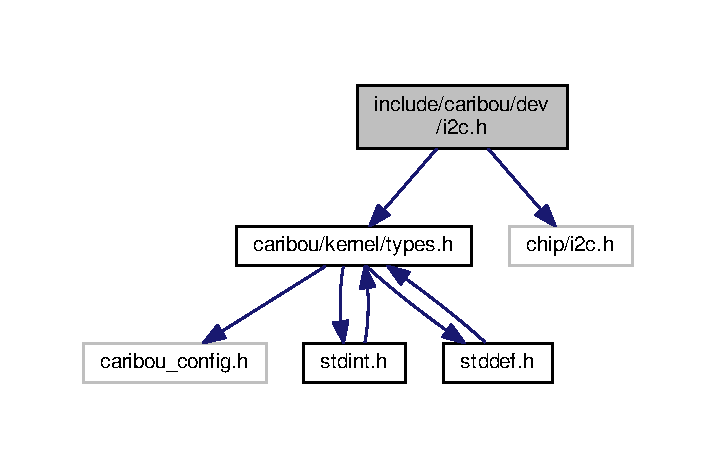
\includegraphics[width=343pt]{i2c_8h__incl}
\end{center}
\end{figure}
This graph shows which files directly or indirectly include this file\-:\nopagebreak
\begin{figure}[H]
\begin{center}
\leavevmode
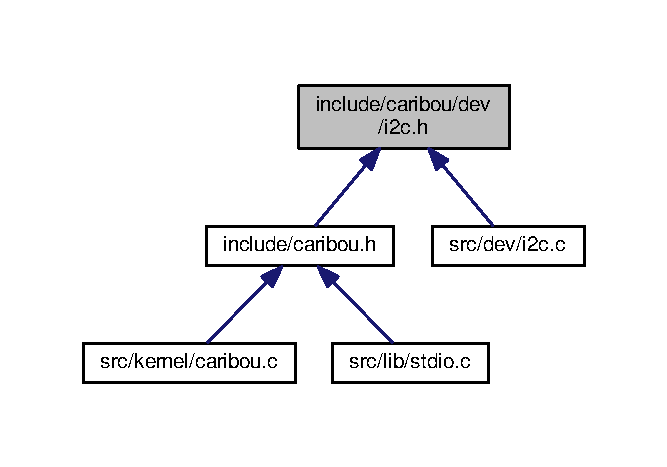
\includegraphics[width=320pt]{i2c_8h__dep__incl}
\end{center}
\end{figure}
\subsection*{Data Structures}
\begin{DoxyCompactItemize}
\item 
struct \hyperlink{structcaribou__i2c__t}{caribou\-\_\-i2c\-\_\-t}
\end{DoxyCompactItemize}
\subsection*{Macros}
\begin{DoxyCompactItemize}
\item 
\#define \hyperlink{i2c_8h_a8ddcbb76f4d8f72464369e33255e81ac}{C\-A\-R\-I\-B\-O\-U\-\_\-\-I2\-C\-\_\-\-I\-N\-I\-T}(port, device\-\_\-address)~\{port,device\-\_\-address\}
\end{DoxyCompactItemize}
\subsection*{Functions}
\begin{DoxyCompactItemize}
\item 
int \hyperlink{i2c_8h_a8f04bf0692d21ae6d8e5c754c677d623}{caribou\-\_\-i2c\-\_\-reset} (\hyperlink{structcaribou__i2c__t}{caribou\-\_\-i2c\-\_\-t} $\ast$i2c)
\item 
int \hyperlink{i2c_8h_ad32ddae7b49ac76182c529b3099c34ca}{caribou\-\_\-i2c\-\_\-tx} (\hyperlink{structcaribou__i2c__t}{caribou\-\_\-i2c\-\_\-t} $\ast$i2c, uint8\-\_\-t $\ast$data, uint8\-\_\-t length)
\begin{DoxyCompactList}\small\item\em Writes a buffer of byte to a specific I2\-C register. \end{DoxyCompactList}\item 
int \hyperlink{i2c_8h_a7e9773a963bd5a08e31d571021244ec3}{caribou\-\_\-i2c\-\_\-rx} (\hyperlink{structcaribou__i2c__t}{caribou\-\_\-i2c\-\_\-t} $\ast$i2c, uint8\-\_\-t $\ast$data, uint8\-\_\-t length)
\begin{DoxyCompactList}\small\item\em Receive a buffer of byte to a specific I2\-C register. \end{DoxyCompactList}\end{DoxyCompactItemize}


\subsection{Detailed Description}




\begin{DoxyAuthor}{Author}
Mike Sharkey \href{mailto:mike@pikeaero.com}{\tt mike@pikeaero.\-com}. 
\end{DoxyAuthor}
\begin{DoxyCopyright}{Copyright}
© 2005-\/2013 by Pike Aerospace Research Corporation 

© 2014-\/2015 by Mike Sharkey
\end{DoxyCopyright}
This file is part of C\-A\-R\-I\-B\-O\-U R\-T\-O\-S C\-A\-R\-I\-B\-O\-U R\-T\-O\-S is free software\-: you can redistribute it and/or modify it under the terms of the Beerware License Version 43. \char`\"{}\-T\-H\-E B\-E\-E\-R-\/\-W\-A\-R\-E L\-I\-C\-E\-N\-S\-E\char`\"{} (Revision 43)\-: Mike Sharkey \href{mailto:mike@pikeaero.com}{\tt mike@pikeaero.\-com} wrote this file. As long as you retain this notice you can do whatever you want with this stuff. If we meet some day, and you think this stuff is worth it, you can buy me a beer in return $\sim$ Mike Sharkey 

Definition in file \hyperlink{i2c_8h_source}{i2c.\-h}.



\subsection{Macro Definition Documentation}
\hypertarget{i2c_8h_a8ddcbb76f4d8f72464369e33255e81ac}{\index{i2c.\-h@{i2c.\-h}!C\-A\-R\-I\-B\-O\-U\-\_\-\-I2\-C\-\_\-\-I\-N\-I\-T@{C\-A\-R\-I\-B\-O\-U\-\_\-\-I2\-C\-\_\-\-I\-N\-I\-T}}
\index{C\-A\-R\-I\-B\-O\-U\-\_\-\-I2\-C\-\_\-\-I\-N\-I\-T@{C\-A\-R\-I\-B\-O\-U\-\_\-\-I2\-C\-\_\-\-I\-N\-I\-T}!i2c.h@{i2c.\-h}}
\subsubsection[{C\-A\-R\-I\-B\-O\-U\-\_\-\-I2\-C\-\_\-\-I\-N\-I\-T}]{\setlength{\rightskip}{0pt plus 5cm}\#define C\-A\-R\-I\-B\-O\-U\-\_\-\-I2\-C\-\_\-\-I\-N\-I\-T(
\begin{DoxyParamCaption}
\item[{}]{port, }
\item[{}]{device\-\_\-address}
\end{DoxyParamCaption}
)~\{port,device\-\_\-address\}}}\label{i2c_8h_a8ddcbb76f4d8f72464369e33255e81ac}


Definition at line 32 of file i2c.\-h.



\subsection{Function Documentation}
\hypertarget{i2c_8h_a8f04bf0692d21ae6d8e5c754c677d623}{\index{i2c.\-h@{i2c.\-h}!caribou\-\_\-i2c\-\_\-reset@{caribou\-\_\-i2c\-\_\-reset}}
\index{caribou\-\_\-i2c\-\_\-reset@{caribou\-\_\-i2c\-\_\-reset}!i2c.h@{i2c.\-h}}
\subsubsection[{caribou\-\_\-i2c\-\_\-reset}]{\setlength{\rightskip}{0pt plus 5cm}int caribou\-\_\-i2c\-\_\-reset (
\begin{DoxyParamCaption}
\item[{{\bf caribou\-\_\-i2c\-\_\-t} $\ast$}]{i2c}
\end{DoxyParamCaption}
)}}\label{i2c_8h_a8f04bf0692d21ae6d8e5c754c677d623}


Definition at line 18 of file i2c.\-c.

\hypertarget{i2c_8h_a7e9773a963bd5a08e31d571021244ec3}{\index{i2c.\-h@{i2c.\-h}!caribou\-\_\-i2c\-\_\-rx@{caribou\-\_\-i2c\-\_\-rx}}
\index{caribou\-\_\-i2c\-\_\-rx@{caribou\-\_\-i2c\-\_\-rx}!i2c.h@{i2c.\-h}}
\subsubsection[{caribou\-\_\-i2c\-\_\-rx}]{\setlength{\rightskip}{0pt plus 5cm}int caribou\-\_\-i2c\-\_\-rx (
\begin{DoxyParamCaption}
\item[{{\bf caribou\-\_\-i2c\-\_\-t} $\ast$}]{i2c, }
\item[{uint8\-\_\-t $\ast$}]{data, }
\item[{uint8\-\_\-t}]{length}
\end{DoxyParamCaption}
)}}\label{i2c_8h_a7e9773a963bd5a08e31d571021244ec3}


Receive a buffer of byte to a specific I2\-C register. 


\begin{DoxyParams}{Parameters}
{\em i2c} & I2\-C device and address. \\
\hline
{\em data} & data to be written to the specific register \\
\hline
{\em length} & data to be written to the specific register \\
\hline
\end{DoxyParams}

\begin{DoxyRetVals}{Return values}
{\em 0x00} & if write operation is O\-K. 0x\-F\-F if timeout condition occured (device not connected or bus error). \\
\hline
\end{DoxyRetVals}


Definition at line 44 of file i2c.\-c.

\hypertarget{i2c_8h_ad32ddae7b49ac76182c529b3099c34ca}{\index{i2c.\-h@{i2c.\-h}!caribou\-\_\-i2c\-\_\-tx@{caribou\-\_\-i2c\-\_\-tx}}
\index{caribou\-\_\-i2c\-\_\-tx@{caribou\-\_\-i2c\-\_\-tx}!i2c.h@{i2c.\-h}}
\subsubsection[{caribou\-\_\-i2c\-\_\-tx}]{\setlength{\rightskip}{0pt plus 5cm}int caribou\-\_\-i2c\-\_\-tx (
\begin{DoxyParamCaption}
\item[{{\bf caribou\-\_\-i2c\-\_\-t} $\ast$}]{i2c, }
\item[{uint8\-\_\-t $\ast$}]{data, }
\item[{uint8\-\_\-t}]{length}
\end{DoxyParamCaption}
)}}\label{i2c_8h_ad32ddae7b49ac76182c529b3099c34ca}


Writes a buffer of byte to a specific I2\-C register. 


\begin{DoxyParams}{Parameters}
{\em i2c} & I2\-C device and address. \\
\hline
{\em data} & data to be written to the specific register \\
\hline
{\em length} & data to be written to the specific register \\
\hline
\end{DoxyParams}

\begin{DoxyRetVals}{Return values}
{\em 0x00} & if write operation is O\-K. 0x\-F\-F if timeout condition occured (device not connected or bus error). \\
\hline
\end{DoxyRetVals}


Definition at line 31 of file i2c.\-c.


\hypertarget{i2s_8h}{\section{include/caribou/dev/i2s.h File Reference}
\label{i2s_8h}\index{include/caribou/dev/i2s.\-h@{include/caribou/dev/i2s.\-h}}
}
{\ttfamily \#include $<$caribou/kernel/types.\-h$>$}\\*
{\ttfamily \#include $<$chip/i2s.\-h$>$}\\*
Include dependency graph for i2s.\-h\-:
\nopagebreak
\begin{figure}[H]
\begin{center}
\leavevmode
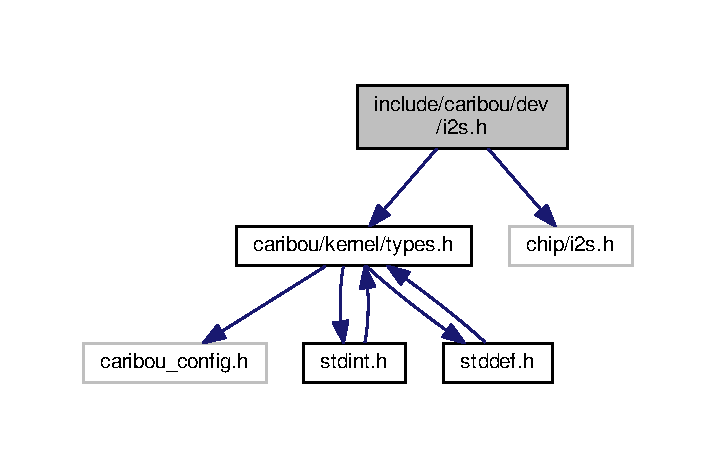
\includegraphics[width=343pt]{i2s_8h__incl}
\end{center}
\end{figure}
This graph shows which files directly or indirectly include this file\-:
\nopagebreak
\begin{figure}[H]
\begin{center}
\leavevmode
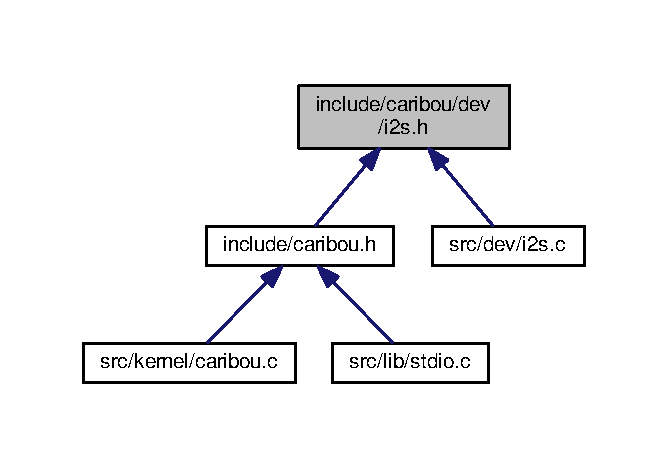
\includegraphics[width=320pt]{i2s_8h__dep__incl}
\end{center}
\end{figure}
\subsection*{Data Structures}
\begin{DoxyCompactItemize}
\item 
struct \hyperlink{structcaribou__i2s__t}{caribou\-\_\-i2s\-\_\-t}
\end{DoxyCompactItemize}
\subsection*{Functions}
\begin{DoxyCompactItemize}
\item 
\hyperlink{types_8h_abb452686968e48b67397da5f97445f5b}{bool} \hyperlink{i2s_8h_ade994a85305aec3403bfe464b5babb09}{caribou\-\_\-i2s\-\_\-rx\-\_\-ready} (\hyperlink{structcaribou__i2s__t}{caribou\-\_\-i2s\-\_\-t} $\ast$i2s)
\item 
chip\-\_\-i2s\-\_\-word\-\_\-t \hyperlink{i2s_8h_a9f20c2cacfd75ff27ac9f99d9b3d772f}{caribou\-\_\-i2s\-\_\-rx} (\hyperlink{structcaribou__i2s__t}{caribou\-\_\-i2s\-\_\-t} $\ast$i2s)
\item 
\hyperlink{types_8h_abb452686968e48b67397da5f97445f5b}{bool} \hyperlink{i2s_8h_a2cec04c7a5e066c24dd50fdda98b44c8}{caribou\-\_\-i2s\-\_\-tx\-\_\-ready} (\hyperlink{structcaribou__i2s__t}{caribou\-\_\-i2s\-\_\-t} $\ast$i2s)
\item 
void \hyperlink{i2s_8h_a0850471149a12ebf5c9ba93a011b8584}{caribou\-\_\-i2s\-\_\-tx} (\hyperlink{structcaribou__i2s__t}{caribou\-\_\-i2s\-\_\-t} $\ast$i2s, chip\-\_\-i2s\-\_\-word\-\_\-t word)
\end{DoxyCompactItemize}


\subsection{Function Documentation}
\hypertarget{i2s_8h_a9f20c2cacfd75ff27ac9f99d9b3d772f}{\index{i2s.\-h@{i2s.\-h}!caribou\-\_\-i2s\-\_\-rx@{caribou\-\_\-i2s\-\_\-rx}}
\index{caribou\-\_\-i2s\-\_\-rx@{caribou\-\_\-i2s\-\_\-rx}!i2s.h@{i2s.\-h}}
\subsubsection[{caribou\-\_\-i2s\-\_\-rx}]{\setlength{\rightskip}{0pt plus 5cm}chip\-\_\-i2s\-\_\-word\-\_\-t caribou\-\_\-i2s\-\_\-rx (
\begin{DoxyParamCaption}
\item[{{\bf caribou\-\_\-i2s\-\_\-t} $\ast$}]{i2s}
\end{DoxyParamCaption}
)}}\label{i2s_8h_a9f20c2cacfd75ff27ac9f99d9b3d772f}


Definition at line 24 of file i2s.\-c.

\hypertarget{i2s_8h_ade994a85305aec3403bfe464b5babb09}{\index{i2s.\-h@{i2s.\-h}!caribou\-\_\-i2s\-\_\-rx\-\_\-ready@{caribou\-\_\-i2s\-\_\-rx\-\_\-ready}}
\index{caribou\-\_\-i2s\-\_\-rx\-\_\-ready@{caribou\-\_\-i2s\-\_\-rx\-\_\-ready}!i2s.h@{i2s.\-h}}
\subsubsection[{caribou\-\_\-i2s\-\_\-rx\-\_\-ready}]{\setlength{\rightskip}{0pt plus 5cm}{\bf bool} caribou\-\_\-i2s\-\_\-rx\-\_\-ready (
\begin{DoxyParamCaption}
\item[{{\bf caribou\-\_\-i2s\-\_\-t} $\ast$}]{i2s}
\end{DoxyParamCaption}
)}}\label{i2s_8h_ade994a85305aec3403bfe464b5babb09}


Definition at line 19 of file i2s.\-c.

\hypertarget{i2s_8h_a0850471149a12ebf5c9ba93a011b8584}{\index{i2s.\-h@{i2s.\-h}!caribou\-\_\-i2s\-\_\-tx@{caribou\-\_\-i2s\-\_\-tx}}
\index{caribou\-\_\-i2s\-\_\-tx@{caribou\-\_\-i2s\-\_\-tx}!i2s.h@{i2s.\-h}}
\subsubsection[{caribou\-\_\-i2s\-\_\-tx}]{\setlength{\rightskip}{0pt plus 5cm}void caribou\-\_\-i2s\-\_\-tx (
\begin{DoxyParamCaption}
\item[{{\bf caribou\-\_\-i2s\-\_\-t} $\ast$}]{i2s, }
\item[{chip\-\_\-i2s\-\_\-word\-\_\-t}]{word}
\end{DoxyParamCaption}
)}}\label{i2s_8h_a0850471149a12ebf5c9ba93a011b8584}


Definition at line 34 of file i2s.\-c.

\hypertarget{i2s_8h_a2cec04c7a5e066c24dd50fdda98b44c8}{\index{i2s.\-h@{i2s.\-h}!caribou\-\_\-i2s\-\_\-tx\-\_\-ready@{caribou\-\_\-i2s\-\_\-tx\-\_\-ready}}
\index{caribou\-\_\-i2s\-\_\-tx\-\_\-ready@{caribou\-\_\-i2s\-\_\-tx\-\_\-ready}!i2s.h@{i2s.\-h}}
\subsubsection[{caribou\-\_\-i2s\-\_\-tx\-\_\-ready}]{\setlength{\rightskip}{0pt plus 5cm}{\bf bool} caribou\-\_\-i2s\-\_\-tx\-\_\-ready (
\begin{DoxyParamCaption}
\item[{{\bf caribou\-\_\-i2s\-\_\-t} $\ast$}]{i2s}
\end{DoxyParamCaption}
)}}\label{i2s_8h_a2cec04c7a5e066c24dd50fdda98b44c8}


Definition at line 29 of file i2s.\-c.


\hypertarget{spi_8h}{\section{include/caribou/dev/spi.h File Reference}
\label{spi_8h}\index{include/caribou/dev/spi.\-h@{include/caribou/dev/spi.\-h}}
}
{\ttfamily \#include $<$caribou/kernel/types.\-h$>$}\\*
{\ttfamily \#include $<$chip/spi.\-h$>$}\\*
Include dependency graph for spi.\-h\-:\nopagebreak
\begin{figure}[H]
\begin{center}
\leavevmode
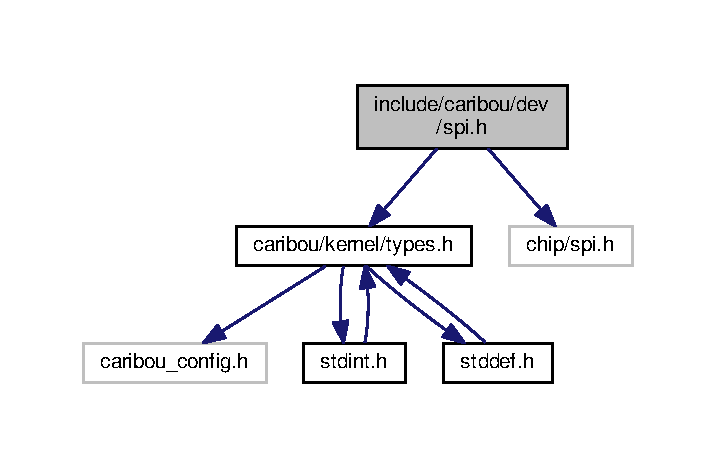
\includegraphics[width=343pt]{spi_8h__incl}
\end{center}
\end{figure}
This graph shows which files directly or indirectly include this file\-:\nopagebreak
\begin{figure}[H]
\begin{center}
\leavevmode
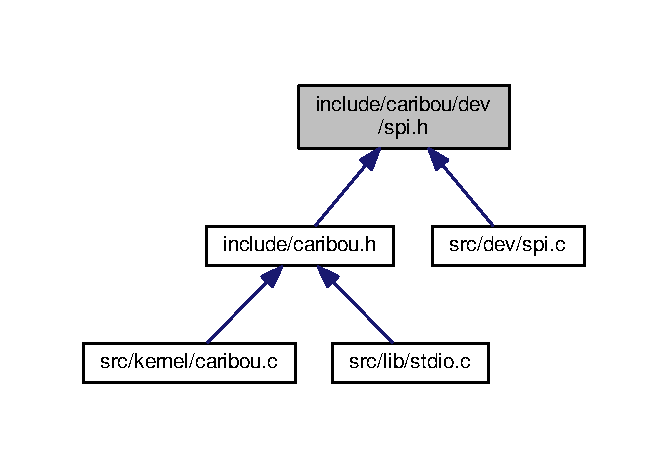
\includegraphics[width=320pt]{spi_8h__dep__incl}
\end{center}
\end{figure}
\subsection*{Data Structures}
\begin{DoxyCompactItemize}
\item 
struct \hyperlink{structcaribou__spi__t}{caribou\-\_\-spi\-\_\-t}
\end{DoxyCompactItemize}
\subsection*{Functions}
\begin{DoxyCompactItemize}
\item 
chip\-\_\-spi\-\_\-word\-\_\-t \hyperlink{spi_8h_a4f479b801ba2ca98458a9033098f00be}{caribou\-\_\-spi\-\_\-exchange} (\hyperlink{structcaribou__spi__t}{caribou\-\_\-spi\-\_\-t} $\ast$spi, chip\-\_\-spi\-\_\-word\-\_\-t word)
\item 
\hyperlink{types_8h_abb452686968e48b67397da5f97445f5b}{bool} \hyperlink{spi_8h_a709caa76439395307b1dbaa74cc2597f}{caribou\-\_\-spi\-\_\-rx\-\_\-ready} (\hyperlink{structcaribou__spi__t}{caribou\-\_\-spi\-\_\-t} $\ast$spi)
\item 
chip\-\_\-spi\-\_\-word\-\_\-t \hyperlink{spi_8h_a1b2aed9c97be43d42062c8ad79e44736}{caribou\-\_\-spi\-\_\-rx} (\hyperlink{structcaribou__spi__t}{caribou\-\_\-spi\-\_\-t} $\ast$spi)
\item 
\hyperlink{types_8h_abb452686968e48b67397da5f97445f5b}{bool} \hyperlink{spi_8h_af33014b48278ba73e4956048b997c6e4}{caribou\-\_\-spi\-\_\-tx\-\_\-ready} (\hyperlink{structcaribou__spi__t}{caribou\-\_\-spi\-\_\-t} $\ast$spi)
\item 
void \hyperlink{spi_8h_a43c558788ae22342f9dbce1dafd89a62}{caribou\-\_\-spi\-\_\-tx} (\hyperlink{structcaribou__spi__t}{caribou\-\_\-spi\-\_\-t} $\ast$spi, chip\-\_\-spi\-\_\-word\-\_\-t word)
\end{DoxyCompactItemize}


\subsection{Detailed Description}




\begin{DoxyAuthor}{Author}
Mike Sharkey \href{mailto:mike@pikeaero.com}{\tt mike@pikeaero.\-com}. 
\end{DoxyAuthor}
\begin{DoxyCopyright}{Copyright}
© 2005-\/2013 by Pike Aerospace Research Corporation 

© 2014-\/2015 by Mike Sharkey
\end{DoxyCopyright}
This file is part of C\-A\-R\-I\-B\-O\-U R\-T\-O\-S C\-A\-R\-I\-B\-O\-U R\-T\-O\-S is free software\-: you can redistribute it and/or modify it under the terms of the Beerware License Version 43. \char`\"{}\-T\-H\-E B\-E\-E\-R-\/\-W\-A\-R\-E L\-I\-C\-E\-N\-S\-E\char`\"{} (Revision 43)\-: Mike Sharkey \href{mailto:mike@pikeaero.com}{\tt mike@pikeaero.\-com} wrote this file. As long as you retain this notice you can do whatever you want with this stuff. If we meet some day, and you think this stuff is worth it, you can buy me a beer in return $\sim$ Mike Sharkey 

Definition in file \hyperlink{spi_8h_source}{spi.\-h}.



\subsection{Function Documentation}
\hypertarget{spi_8h_a4f479b801ba2ca98458a9033098f00be}{\index{spi.\-h@{spi.\-h}!caribou\-\_\-spi\-\_\-exchange@{caribou\-\_\-spi\-\_\-exchange}}
\index{caribou\-\_\-spi\-\_\-exchange@{caribou\-\_\-spi\-\_\-exchange}!spi.h@{spi.\-h}}
\subsubsection[{caribou\-\_\-spi\-\_\-exchange}]{\setlength{\rightskip}{0pt plus 5cm}chip\-\_\-spi\-\_\-word\-\_\-t caribou\-\_\-spi\-\_\-exchange (
\begin{DoxyParamCaption}
\item[{{\bf caribou\-\_\-spi\-\_\-t} $\ast$}]{spi, }
\item[{chip\-\_\-spi\-\_\-word\-\_\-t}]{word}
\end{DoxyParamCaption}
)}}\label{spi_8h_a4f479b801ba2ca98458a9033098f00be}


Definition at line 17 of file spi.\-c.

\hypertarget{spi_8h_a1b2aed9c97be43d42062c8ad79e44736}{\index{spi.\-h@{spi.\-h}!caribou\-\_\-spi\-\_\-rx@{caribou\-\_\-spi\-\_\-rx}}
\index{caribou\-\_\-spi\-\_\-rx@{caribou\-\_\-spi\-\_\-rx}!spi.h@{spi.\-h}}
\subsubsection[{caribou\-\_\-spi\-\_\-rx}]{\setlength{\rightskip}{0pt plus 5cm}chip\-\_\-spi\-\_\-word\-\_\-t caribou\-\_\-spi\-\_\-rx (
\begin{DoxyParamCaption}
\item[{{\bf caribou\-\_\-spi\-\_\-t} $\ast$}]{spi}
\end{DoxyParamCaption}
)}}\label{spi_8h_a1b2aed9c97be43d42062c8ad79e44736}


Definition at line 27 of file spi.\-c.

\hypertarget{spi_8h_a709caa76439395307b1dbaa74cc2597f}{\index{spi.\-h@{spi.\-h}!caribou\-\_\-spi\-\_\-rx\-\_\-ready@{caribou\-\_\-spi\-\_\-rx\-\_\-ready}}
\index{caribou\-\_\-spi\-\_\-rx\-\_\-ready@{caribou\-\_\-spi\-\_\-rx\-\_\-ready}!spi.h@{spi.\-h}}
\subsubsection[{caribou\-\_\-spi\-\_\-rx\-\_\-ready}]{\setlength{\rightskip}{0pt plus 5cm}{\bf bool} caribou\-\_\-spi\-\_\-rx\-\_\-ready (
\begin{DoxyParamCaption}
\item[{{\bf caribou\-\_\-spi\-\_\-t} $\ast$}]{spi}
\end{DoxyParamCaption}
)}}\label{spi_8h_a709caa76439395307b1dbaa74cc2597f}


Definition at line 22 of file spi.\-c.

\hypertarget{spi_8h_a43c558788ae22342f9dbce1dafd89a62}{\index{spi.\-h@{spi.\-h}!caribou\-\_\-spi\-\_\-tx@{caribou\-\_\-spi\-\_\-tx}}
\index{caribou\-\_\-spi\-\_\-tx@{caribou\-\_\-spi\-\_\-tx}!spi.h@{spi.\-h}}
\subsubsection[{caribou\-\_\-spi\-\_\-tx}]{\setlength{\rightskip}{0pt plus 5cm}void caribou\-\_\-spi\-\_\-tx (
\begin{DoxyParamCaption}
\item[{{\bf caribou\-\_\-spi\-\_\-t} $\ast$}]{spi, }
\item[{chip\-\_\-spi\-\_\-word\-\_\-t}]{word}
\end{DoxyParamCaption}
)}}\label{spi_8h_a43c558788ae22342f9dbce1dafd89a62}


Definition at line 37 of file spi.\-c.

\hypertarget{spi_8h_af33014b48278ba73e4956048b997c6e4}{\index{spi.\-h@{spi.\-h}!caribou\-\_\-spi\-\_\-tx\-\_\-ready@{caribou\-\_\-spi\-\_\-tx\-\_\-ready}}
\index{caribou\-\_\-spi\-\_\-tx\-\_\-ready@{caribou\-\_\-spi\-\_\-tx\-\_\-ready}!spi.h@{spi.\-h}}
\subsubsection[{caribou\-\_\-spi\-\_\-tx\-\_\-ready}]{\setlength{\rightskip}{0pt plus 5cm}{\bf bool} caribou\-\_\-spi\-\_\-tx\-\_\-ready (
\begin{DoxyParamCaption}
\item[{{\bf caribou\-\_\-spi\-\_\-t} $\ast$}]{spi}
\end{DoxyParamCaption}
)}}\label{spi_8h_af33014b48278ba73e4956048b997c6e4}


Definition at line 32 of file spi.\-c.


\hypertarget{uart_8h}{\section{include/caribou/dev/uart.h File Reference}
\label{uart_8h}\index{include/caribou/dev/uart.\-h@{include/caribou/dev/uart.\-h}}
}
{\ttfamily \#include $<$caribou/kernel/types.\-h$>$}\\*
{\ttfamily \#include $<$caribou/lib/bytequeue.\-h$>$}\\*
{\ttfamily \#include $<$chip/uart.\-h$>$}\\*
Include dependency graph for uart.\-h\-:
\nopagebreak
\begin{figure}[H]
\begin{center}
\leavevmode
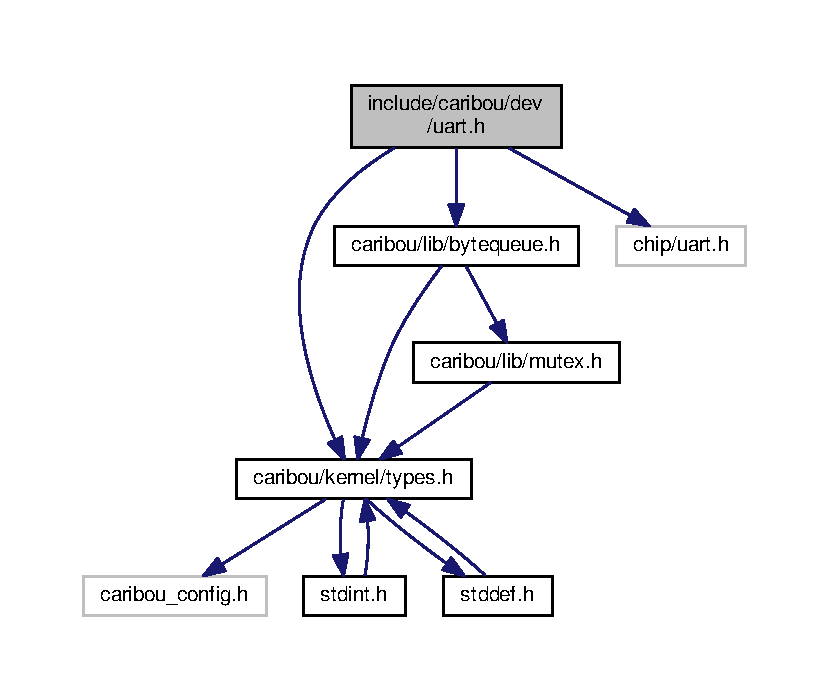
\includegraphics[width=350pt]{uart_8h__incl}
\end{center}
\end{figure}
This graph shows which files directly or indirectly include this file\-:
\nopagebreak
\begin{figure}[H]
\begin{center}
\leavevmode
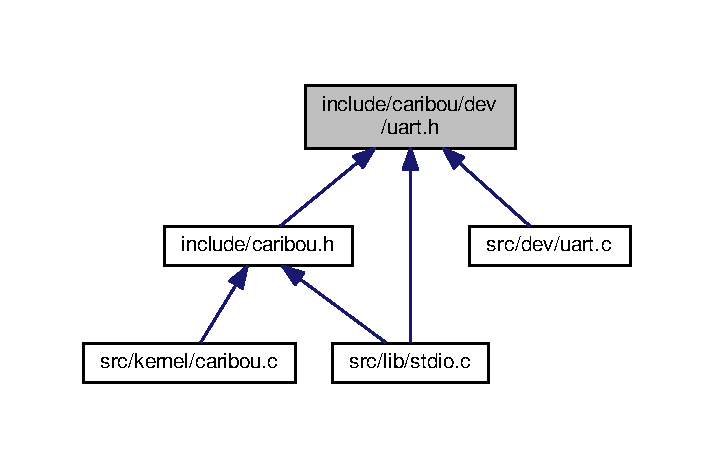
\includegraphics[width=342pt]{uart_8h__dep__incl}
\end{center}
\end{figure}
\subsection*{Data Structures}
\begin{DoxyCompactItemize}
\item 
struct \hyperlink{structcaribou__uart__config__t}{caribou\-\_\-uart\-\_\-config\-\_\-t}
\end{DoxyCompactItemize}
\subsection*{Macros}
\begin{DoxyCompactItemize}
\item 
\#define \hyperlink{uart_8h_a87464c2386112c114242554dc2d50a59}{C\-A\-R\-I\-B\-O\-U\-\_\-\-U\-A\-R\-T\-\_\-\-C\-O\-N\-F\-I\-G\-\_\-\-I\-N\-I\-T}
\end{DoxyCompactItemize}
\subsection*{Enumerations}
\begin{DoxyCompactItemize}
\item 
enum \hyperlink{uart_8h_afef1566c0e2499ac54d03f9840e67367}{caribou\-\_\-uart\-\_\-baud\-\_\-t} \{ \\*
\hyperlink{uart_8h_afef1566c0e2499ac54d03f9840e67367a7c7aa50563352ad101cd967943773708}{C\-A\-R\-I\-B\-O\-U\-\_\-\-U\-A\-R\-T\-\_\-\-B\-A\-U\-D\-\_\-\-R\-A\-T\-E\-\_\-110} =110, 
\hyperlink{uart_8h_afef1566c0e2499ac54d03f9840e67367a2bac6d98eadc4832fe7a25a64eaa6d59}{C\-A\-R\-I\-B\-O\-U\-\_\-\-U\-A\-R\-T\-\_\-\-B\-A\-U\-D\-\_\-\-R\-A\-T\-E\-\_\-300} =300, 
\hyperlink{uart_8h_afef1566c0e2499ac54d03f9840e67367ab9b3dab63db80d5ed9f1715adb299e81}{C\-A\-R\-I\-B\-O\-U\-\_\-\-U\-A\-R\-T\-\_\-\-B\-A\-U\-D\-\_\-\-R\-A\-T\-E\-\_\-600} =600, 
\hyperlink{uart_8h_afef1566c0e2499ac54d03f9840e67367aed69f4a9228e9117d94c4d1a2a893a8d}{C\-A\-R\-I\-B\-O\-U\-\_\-\-U\-A\-R\-T\-\_\-\-B\-A\-U\-D\-\_\-\-R\-A\-T\-E\-\_\-1200} =1200, 
\\*
\hyperlink{uart_8h_afef1566c0e2499ac54d03f9840e67367ac2cbc9a189c9f7b4d55d0e638f3033cc}{C\-A\-R\-I\-B\-O\-U\-\_\-\-U\-A\-R\-T\-\_\-\-B\-A\-U\-D\-\_\-\-R\-A\-T\-E\-\_\-2400} =2400, 
\hyperlink{uart_8h_afef1566c0e2499ac54d03f9840e67367a0f967e0b954be3870b61f1721b97f779}{C\-A\-R\-I\-B\-O\-U\-\_\-\-U\-A\-R\-T\-\_\-\-B\-A\-U\-D\-\_\-\-R\-A\-T\-E\-\_\-4800} =4800, 
\hyperlink{uart_8h_afef1566c0e2499ac54d03f9840e67367a862e692083ac7312721985f91a5b731e}{C\-A\-R\-I\-B\-O\-U\-\_\-\-U\-A\-R\-T\-\_\-\-B\-A\-U\-D\-\_\-\-R\-A\-T\-E\-\_\-9600} =9600, 
\hyperlink{uart_8h_afef1566c0e2499ac54d03f9840e67367a3f9fa370672d8e25f28747b5153abffa}{C\-A\-R\-I\-B\-O\-U\-\_\-\-U\-A\-R\-T\-\_\-\-B\-A\-U\-D\-\_\-\-R\-A\-T\-E\-\_\-19200} =19200, 
\\*
\hyperlink{uart_8h_afef1566c0e2499ac54d03f9840e67367abb9dc1d19a17d9648fc20abf42323eb1}{C\-A\-R\-I\-B\-O\-U\-\_\-\-U\-A\-R\-T\-\_\-\-B\-A\-U\-D\-\_\-\-R\-A\-T\-E\-\_\-28800} =28800, 
\hyperlink{uart_8h_afef1566c0e2499ac54d03f9840e67367ab1794f1c7b8352bcdd8546dd219c580e}{C\-A\-R\-I\-B\-O\-U\-\_\-\-U\-A\-R\-T\-\_\-\-B\-A\-U\-D\-\_\-\-R\-A\-T\-E\-\_\-38400} =38400, 
\hyperlink{uart_8h_afef1566c0e2499ac54d03f9840e67367ab32258b3765fa22110a5fbd5775a2d9a}{C\-A\-R\-I\-B\-O\-U\-\_\-\-U\-A\-R\-T\-\_\-\-B\-A\-U\-D\-\_\-\-R\-A\-T\-E\-\_\-56000} =56000, 
\hyperlink{uart_8h_afef1566c0e2499ac54d03f9840e67367a3c41f810ccb201769b65335fcc13dac5}{C\-A\-R\-I\-B\-O\-U\-\_\-\-U\-A\-R\-T\-\_\-\-B\-A\-U\-D\-\_\-\-R\-A\-T\-E\-\_\-57600} =57600, 
\\*
\hyperlink{uart_8h_afef1566c0e2499ac54d03f9840e67367a3e04c055b1b9abb15892394e9cf5fb23}{C\-A\-R\-I\-B\-O\-U\-\_\-\-U\-A\-R\-T\-\_\-\-B\-A\-U\-D\-\_\-\-R\-A\-T\-E\-\_\-115200} =115200, 
\hyperlink{uart_8h_afef1566c0e2499ac54d03f9840e67367a8757741e77d96d0b3ef5af9d6c3533f4}{C\-A\-R\-I\-B\-O\-U\-\_\-\-U\-A\-R\-T\-\_\-\-B\-A\-U\-D\-\_\-\-R\-A\-T\-E\-\_\-128000} =128000, 
\hyperlink{uart_8h_afef1566c0e2499ac54d03f9840e67367a7d7f1723764e254106f84e5e75115c8c}{C\-A\-R\-I\-B\-O\-U\-\_\-\-U\-A\-R\-T\-\_\-\-B\-A\-U\-D\-\_\-\-R\-A\-T\-E\-\_\-153600} =153600, 
\hyperlink{uart_8h_afef1566c0e2499ac54d03f9840e67367a870b99daf9141d33c9c3d9bde9d3bd62}{C\-A\-R\-I\-B\-O\-U\-\_\-\-U\-A\-R\-T\-\_\-\-B\-A\-U\-D\-\_\-\-R\-A\-T\-E\-\_\-230400} =230400, 
\\*
\hyperlink{uart_8h_afef1566c0e2499ac54d03f9840e67367a6e7f4c98e362827d072ba2b33e95e647}{C\-A\-R\-I\-B\-O\-U\-\_\-\-U\-A\-R\-T\-\_\-\-B\-A\-U\-D\-\_\-\-R\-A\-T\-E\-\_\-256000} =256000, 
\hyperlink{uart_8h_afef1566c0e2499ac54d03f9840e67367af0d78e4b80403f7fd62302e81140e2e9}{C\-A\-R\-I\-B\-O\-U\-\_\-\-U\-A\-R\-T\-\_\-\-B\-A\-U\-D\-\_\-\-R\-A\-T\-E\-\_\-460800} =460800, 
\hyperlink{uart_8h_afef1566c0e2499ac54d03f9840e67367a6ccf6b4a1da8cc0f91f59471ab27e8c8}{C\-A\-R\-I\-B\-O\-U\-\_\-\-U\-A\-R\-T\-\_\-\-B\-A\-U\-D\-\_\-\-R\-A\-T\-E\-\_\-921600} =921600, 
\hyperlink{uart_8h_afef1566c0e2499ac54d03f9840e67367a4a1422b187fbcfcd5c9aa320b608fb16}{C\-A\-R\-I\-B\-O\-U\-\_\-\-U\-A\-R\-T\-\_\-\-B\-A\-U\-D\-\_\-\-R\-A\-T\-E\-\_\-1792000} =1792000, 
\\*
\hyperlink{uart_8h_afef1566c0e2499ac54d03f9840e67367a2b37069e6577cad01ecafbe2e18659d4}{C\-A\-R\-I\-B\-O\-U\-\_\-\-U\-A\-R\-T\-\_\-\-B\-A\-U\-D\-\_\-\-R\-A\-T\-E\-\_\-1843200} =1843200, 
\hyperlink{uart_8h_afef1566c0e2499ac54d03f9840e67367abb429b0ba93c818098f1e5c9d700cea1}{C\-A\-R\-I\-B\-O\-U\-\_\-\-U\-A\-R\-T\-\_\-\-B\-A\-U\-D\-\_\-\-R\-A\-T\-E\-\_\-3584000} =3584000, 
\hyperlink{uart_8h_afef1566c0e2499ac54d03f9840e67367a53fedd8a1f89e06584e0633ed617f615}{C\-A\-R\-I\-B\-O\-U\-\_\-\-U\-A\-R\-T\-\_\-\-B\-A\-U\-D\-\_\-\-R\-A\-T\-E\-\_\-3686400} =3686400, 
\hyperlink{uart_8h_afef1566c0e2499ac54d03f9840e67367a9f18d401efa38d01abdfa6c788772ee3}{C\-A\-R\-I\-B\-O\-U\-\_\-\-U\-A\-R\-T\-\_\-\-B\-A\-U\-D\-\_\-\-R\-A\-T\-E\-\_\-7168000} =7168000, 
\\*
\hyperlink{uart_8h_afef1566c0e2499ac54d03f9840e67367a2cf083a934a14c297f2a1477d9df1c76}{C\-A\-R\-I\-B\-O\-U\-\_\-\-U\-A\-R\-T\-\_\-\-B\-A\-U\-D\-\_\-\-R\-A\-T\-E\-\_\-7372800} =7372800, 
\hyperlink{uart_8h_afef1566c0e2499ac54d03f9840e67367a3fbb897f644c7ce208ab82dd9e16109f}{C\-A\-R\-I\-B\-O\-U\-\_\-\-U\-A\-R\-T\-\_\-\-B\-A\-U\-D\-\_\-\-R\-A\-T\-E\-\_\-9000000} =9000000, 
\hyperlink{uart_8h_afef1566c0e2499ac54d03f9840e67367a7e20810091b10ecf78e1d7f0796d3a3a}{C\-A\-R\-I\-B\-O\-U\-\_\-\-U\-A\-R\-T\-\_\-\-B\-A\-U\-D\-\_\-\-R\-A\-T\-E\-\_\-10500000} =10500000
 \}
\item 
enum \hyperlink{uart_8h_a9a6df27e70711dcf554553bcd934cdf9}{caribou\-\_\-uart\-\_\-word\-\_\-t} \{ \\*
\hyperlink{uart_8h_a9a6df27e70711dcf554553bcd934cdf9a816d7d1206a07f1d7121c5460555646d}{C\-A\-R\-I\-B\-O\-U\-\_\-\-U\-A\-R\-T\-\_\-\-W\-O\-R\-D\-S\-I\-Z\-E\-\_\-5} =5, 
\hyperlink{uart_8h_a9a6df27e70711dcf554553bcd934cdf9a8796a9fc8b686991b70d65ff407c5b0c}{C\-A\-R\-I\-B\-O\-U\-\_\-\-U\-A\-R\-T\-\_\-\-W\-O\-R\-D\-S\-I\-Z\-E\-\_\-6} =6, 
\hyperlink{uart_8h_a9a6df27e70711dcf554553bcd934cdf9aeb24d5063eced3c39691e98c0d78e7b5}{C\-A\-R\-I\-B\-O\-U\-\_\-\-U\-A\-R\-T\-\_\-\-W\-O\-R\-D\-S\-I\-Z\-E\-\_\-7} =7, 
\hyperlink{uart_8h_a9a6df27e70711dcf554553bcd934cdf9ab93799ce8ae17c9a474e6b4d514cbdbe}{C\-A\-R\-I\-B\-O\-U\-\_\-\-U\-A\-R\-T\-\_\-\-W\-O\-R\-D\-S\-I\-Z\-E\-\_\-8} =8, 
\\*
\hyperlink{uart_8h_a9a6df27e70711dcf554553bcd934cdf9a7c29af0b17c3b27f5f9eb6d6edb65ae6}{C\-A\-R\-I\-B\-O\-U\-\_\-\-U\-A\-R\-T\-\_\-\-W\-O\-R\-D\-S\-I\-Z\-E\-\_\-9} =9
 \}
\item 
enum \hyperlink{uart_8h_a8a7a8a9e91ed00784943f12dd2b3825e}{caribou\-\_\-uart\-\_\-stop\-\_\-t} \{ \hyperlink{uart_8h_a8a7a8a9e91ed00784943f12dd2b3825ea396168b624f7764f870e269bf665b64a}{C\-A\-R\-I\-B\-O\-U\-\_\-\-U\-A\-R\-T\-\_\-\-S\-T\-O\-P\-B\-I\-T\-S\-\_\-05}, 
\hyperlink{uart_8h_a8a7a8a9e91ed00784943f12dd2b3825ea3f1bb393a6e4b9f3e4777533706fe655}{C\-A\-R\-I\-B\-O\-U\-\_\-\-U\-A\-R\-T\-\_\-\-S\-T\-O\-P\-B\-I\-T\-S\-\_\-1}, 
\hyperlink{uart_8h_a8a7a8a9e91ed00784943f12dd2b3825ea840d9501b273f7adf6d8ffa529742637}{C\-A\-R\-I\-B\-O\-U\-\_\-\-U\-A\-R\-T\-\_\-\-S\-T\-O\-P\-B\-I\-T\-S\-\_\-15}, 
\hyperlink{uart_8h_a8a7a8a9e91ed00784943f12dd2b3825ea9f339a88fcf6eb31c013936286f70082}{C\-A\-R\-I\-B\-O\-U\-\_\-\-U\-A\-R\-T\-\_\-\-S\-T\-O\-P\-B\-I\-T\-S\-\_\-2}
 \}
\item 
enum \hyperlink{uart_8h_a21331436e5b880d78970abb6dbfad09b}{caribou\-\_\-uart\-\_\-parity\-\_\-t} \{ \hyperlink{uart_8h_a21331436e5b880d78970abb6dbfad09baaa486a3921a625c92c05227e5bcaecfe}{C\-A\-R\-I\-B\-O\-U\-\_\-\-U\-A\-R\-T\-\_\-\-P\-A\-R\-I\-T\-Y\-\_\-\-N\-O\-N\-E}, 
\hyperlink{uart_8h_a21331436e5b880d78970abb6dbfad09ba4d5381188947235ed8c90bfb6f8b21ab}{C\-A\-R\-I\-B\-O\-U\-\_\-\-U\-A\-R\-T\-\_\-\-P\-A\-R\-I\-T\-Y\-\_\-\-E\-V\-E\-N}, 
\hyperlink{uart_8h_a21331436e5b880d78970abb6dbfad09ba2d3593c77b7123eaa57622965f06c55d}{C\-A\-R\-I\-B\-O\-U\-\_\-\-U\-A\-R\-T\-\_\-\-P\-A\-R\-I\-T\-Y\-\_\-\-O\-D\-D}
 \}
\item 
enum \hyperlink{uart_8h_a54948edc934015197b158136f30a074d}{caribou\-\_\-uart\-\_\-flow\-\_\-t} \{ \hyperlink{uart_8h_a54948edc934015197b158136f30a074da8ece57db197db532d5a1dfc0102af287}{C\-A\-R\-I\-B\-O\-U\-\_\-\-U\-A\-R\-T\-\_\-\-F\-L\-O\-W\-\_\-\-N\-O\-N\-E} =0, 
\hyperlink{uart_8h_a54948edc934015197b158136f30a074da15308d60d2a73f978580f98ecc4d4e87}{C\-A\-R\-I\-B\-O\-U\-\_\-\-U\-A\-R\-T\-\_\-\-F\-L\-O\-W\-\_\-\-R\-T\-S} =0x01, 
\hyperlink{uart_8h_a54948edc934015197b158136f30a074da289fce8620ee5505b4a008e740b0d18d}{C\-A\-R\-I\-B\-O\-U\-\_\-\-U\-A\-R\-T\-\_\-\-F\-L\-O\-W\-\_\-\-C\-T\-S} =0x02, 
\hyperlink{uart_8h_a54948edc934015197b158136f30a074dab3756cab6d0d063f95cda3b4a5c41aaf}{C\-A\-R\-I\-B\-O\-U\-\_\-\-U\-A\-R\-T\-\_\-\-F\-L\-O\-W\-\_\-\-R\-T\-S\-\_\-\-C\-T\-S} =0x03
 \}
\end{DoxyCompactItemize}
\subsection*{Functions}
\begin{DoxyCompactItemize}
\item 
int \hyperlink{uart_8h_a9a85b0c56dbc7199c9608979903272ab}{caribou\-\_\-uart\-\_\-open} (int devicenum, \hyperlink{structcaribou__uart__config__t}{caribou\-\_\-uart\-\_\-config\-\_\-t} $\ast$config)
\begin{DoxyCompactList}\small\item\em Open a U\-A\-R\-T device for subsequent use. \end{DoxyCompactList}\item 
void \hyperlink{uart_8h_a93b1a50c466b5579ee6080cd378114b6}{caribou\-\_\-uart\-\_\-init\-\_\-config} (\hyperlink{structcaribou__uart__config__t}{caribou\-\_\-uart\-\_\-config\-\_\-t} $\ast$config)
\begin{DoxyCompactList}\small\item\em Initialize the config record to contain sane values. \end{DoxyCompactList}\item 
int \hyperlink{uart_8h_a95be81c80a3d8d897177069628a7b18f}{caribou\-\_\-uart\-\_\-set\-\_\-config} (int fd, \hyperlink{structcaribou__uart__config__t}{caribou\-\_\-uart\-\_\-config\-\_\-t} $\ast$config)
\begin{DoxyCompactList}\small\item\em Set the U\-A\-R\-T configuration. \end{DoxyCompactList}\item 
int \hyperlink{uart_8h_a69c58ec3847a900168737c43dec3fcbc}{caribou\-\_\-uart\-\_\-close} (int fd)
\begin{DoxyCompactList}\small\item\em Close a previously opened U\-A\-R\-T. \end{DoxyCompactList}\item 
int \hyperlink{uart_8h_a64d85da5442a9faeeae387fc7f971412}{caribou\-\_\-uart\-\_\-int\-\_\-enable} (int fd)
\begin{DoxyCompactList}\small\item\em Enable U\-A\-R\-T interrupts. \end{DoxyCompactList}\item 
int \hyperlink{uart_8h_a5fb29fdb37419d5e8f37beafe6075322}{caribou\-\_\-uart\-\_\-int\-\_\-disable} (int fd)
\begin{DoxyCompactList}\small\item\em Disable U\-A\-R\-T interrupts. \end{DoxyCompactList}\item 
int \hyperlink{uart_8h_a6a4f7e52bda927444a0b0fa1af205651}{caribou\-\_\-uart\-\_\-int\-\_\-enabled} (int fd)
\begin{DoxyCompactList}\small\item\em Determine if the U\-A\-R\-T interrupts are enabled. \end{DoxyCompactList}\item 
int \hyperlink{uart_8h_a022166fd5acba50d49188e433eca93e0}{caribou\-\_\-uart\-\_\-int\-\_\-set} (int fd, int state)
\begin{DoxyCompactList}\small\item\em Set the U\-A\-R\-T interrupt state. \end{DoxyCompactList}\item 
\hyperlink{structcaribou__bytequeue__t}{caribou\-\_\-bytequeue\-\_\-t} $\ast$ \hyperlink{uart_8h_a8b7d4543a230f68ca97188aa64da2ad1}{caribou\-\_\-uart\-\_\-rx\-\_\-queue} (int fd)
\item 
\hyperlink{structcaribou__bytequeue__t}{caribou\-\_\-bytequeue\-\_\-t} $\ast$ \hyperlink{uart_8h_a6b2993300e7c152eb6cc992feaf98c9a}{caribou\-\_\-uart\-\_\-tx\-\_\-queue} (int fd)
\item 
void \hyperlink{uart_8h_ac60f61b823d817b68cf858a7404980ea}{caribou\-\_\-uart\-\_\-enable} (int fd)
\item 
void \hyperlink{uart_8h_a52579b7ba4ba9c9b36f770e12d26de65}{caribou\-\_\-uart\-\_\-disable} (int fd)
\item 
int \hyperlink{uart_8h_a297914e4527fd034ffbf95c740d2f37f}{caribou\-\_\-uart\-\_\-queue\-\_\-tx\-\_\-sz} ()
\item 
int \hyperlink{uart_8h_a351e35bbfed47860d7f40fb1fba387be}{caribou\-\_\-uart\-\_\-queue\-\_\-rx\-\_\-sz} ()
\item 
int \hyperlink{uart_8h_ad763845504097b6d6debe7ec52f60fb3}{caribou\-\_\-uart\-\_\-tx\-\_\-data} (int fd, int ch)
\begin{DoxyCompactList}\small\item\em Place a byte into the U\-A\-R\-T transmit buffer. \end{DoxyCompactList}\item 
int \hyperlink{uart_8h_a0a8cbc25e619395ae7c4de7895da3a41}{caribou\-\_\-uart\-\_\-rx\-\_\-data} (int fd)
\begin{DoxyCompactList}\small\item\em Retrieve a byte from the U\-A\-R\-T holding register. \end{DoxyCompactList}\item 
\hyperlink{types_8h_abb452686968e48b67397da5f97445f5b}{bool} \hyperlink{uart_8h_ac598aa7ccb4824abe80296502d27ec86}{caribou\-\_\-uart\-\_\-tx\-\_\-busy} (int fd)
\begin{DoxyCompactList}\small\item\em Determine of the U\-A\-R\-T transmitter is busy. \end{DoxyCompactList}\item 
\hyperlink{types_8h_abb452686968e48b67397da5f97445f5b}{bool} \hyperlink{uart_8h_af3210bdc9cd62075c0143b639c581772}{caribou\-\_\-uart\-\_\-tx\-\_\-ready} (int fd)
\begin{DoxyCompactList}\small\item\em Determine of the U\-A\-R\-T transmitter is ready to accept a byte. \end{DoxyCompactList}\item 
\hyperlink{types_8h_abb452686968e48b67397da5f97445f5b}{bool} \hyperlink{uart_8h_aa82184396ed62090414e5bd4f3d3ab0c}{caribou\-\_\-uart\-\_\-rx\-\_\-ready} (int fd)
\begin{DoxyCompactList}\small\item\em Determine of receiver has data ready. \end{DoxyCompactList}\item 
int \hyperlink{uart_8h_afaed2785671eb5acc7df6c3efe1c1515}{caribou\-\_\-uart\-\_\-private\-\_\-readfn} (\hyperlink{stdio_8h_a137c2fc14236952cafc759ada2bb2d8a}{stdio\-\_\-t} $\ast$io, void $\ast$data, int count)
\begin{DoxyCompactList}\small\item\em F\-I\-X\-M\-E make really private declarations. \end{DoxyCompactList}\item 
int \hyperlink{uart_8h_a5f7ddc5c012cb9967d9053f3b5b3c8a3}{caribou\-\_\-uart\-\_\-private\-\_\-writefn} (\hyperlink{stdio_8h_a137c2fc14236952cafc759ada2bb2d8a}{stdio\-\_\-t} $\ast$io, void $\ast$data, int count)
\begin{DoxyCompactList}\small\item\em Device Driver read-\/data function. \end{DoxyCompactList}\item 
int \hyperlink{uart_8h_a104d19d00c26c184eb6b352539b146a8}{caribou\-\_\-uart\-\_\-private\-\_\-readqueuefn} (\hyperlink{stdio_8h_a137c2fc14236952cafc759ada2bb2d8a}{stdio\-\_\-t} $\ast$io)
\begin{DoxyCompactList}\small\item\em Device Driver write-\/data function. \end{DoxyCompactList}\item 
int \hyperlink{uart_8h_a133b9c5413db93d9d99fefc550dbd2ab}{caribou\-\_\-uart\-\_\-private\-\_\-writequeuefn} (\hyperlink{stdio_8h_a137c2fc14236952cafc759ada2bb2d8a}{stdio\-\_\-t} $\ast$io)
\begin{DoxyCompactList}\small\item\em Device Driver read-\/data available function. \end{DoxyCompactList}\item 
int \hyperlink{uart_8h_ad888daa7223dda1848704a8ddf83df5d}{caribou\-\_\-uart\-\_\-private\-\_\-statefn} (\hyperlink{stdio_8h_a137c2fc14236952cafc759ada2bb2d8a}{stdio\-\_\-t} $\ast$io)
\begin{DoxyCompactList}\small\item\em Device Driver write-\/data pending. \end{DoxyCompactList}\end{DoxyCompactItemize}


\subsection{Macro Definition Documentation}
\hypertarget{uart_8h_a87464c2386112c114242554dc2d50a59}{\index{uart.\-h@{uart.\-h}!C\-A\-R\-I\-B\-O\-U\-\_\-\-U\-A\-R\-T\-\_\-\-C\-O\-N\-F\-I\-G\-\_\-\-I\-N\-I\-T@{C\-A\-R\-I\-B\-O\-U\-\_\-\-U\-A\-R\-T\-\_\-\-C\-O\-N\-F\-I\-G\-\_\-\-I\-N\-I\-T}}
\index{C\-A\-R\-I\-B\-O\-U\-\_\-\-U\-A\-R\-T\-\_\-\-C\-O\-N\-F\-I\-G\-\_\-\-I\-N\-I\-T@{C\-A\-R\-I\-B\-O\-U\-\_\-\-U\-A\-R\-T\-\_\-\-C\-O\-N\-F\-I\-G\-\_\-\-I\-N\-I\-T}!uart.h@{uart.\-h}}
\subsubsection[{C\-A\-R\-I\-B\-O\-U\-\_\-\-U\-A\-R\-T\-\_\-\-C\-O\-N\-F\-I\-G\-\_\-\-I\-N\-I\-T}]{\setlength{\rightskip}{0pt plus 5cm}\#define C\-A\-R\-I\-B\-O\-U\-\_\-\-U\-A\-R\-T\-\_\-\-C\-O\-N\-F\-I\-G\-\_\-\-I\-N\-I\-T}}\label{uart_8h_a87464c2386112c114242554dc2d50a59}
{\bfseries Value\-:}
\begin{DoxyCode}
\{ \hyperlink{uart_8h_afef1566c0e2499ac54d03f9840e67367a862e692083ac7312721985f91a5b731e}{CARIBOU\_UART\_BAUD\_RATE\_9600}, \hyperlink{uart_8h_a9a6df27e70711dcf554553bcd934cdf9ab93799ce8ae17c9a474e6b4d514cbdbe}{\(\backslash\)}
\hyperlink{uart_8h_a9a6df27e70711dcf554553bcd934cdf9ab93799ce8ae17c9a474e6b4d514cbdbe}{                                   CARIBOU\_UART\_WORDSIZE\_8},       
      \hyperlink{uart_8h_a8a7a8a9e91ed00784943f12dd2b3825ea3f1bb393a6e4b9f3e4777533706fe655}{\(\backslash\)}
\hyperlink{uart_8h_a8a7a8a9e91ed00784943f12dd2b3825ea3f1bb393a6e4b9f3e4777533706fe655}{                                   CARIBOU\_UART\_STOPBITS\_1},       
      \hyperlink{uart_8h_a21331436e5b880d78970abb6dbfad09baaa486a3921a625c92c05227e5bcaecfe}{\(\backslash\)}
\hyperlink{uart_8h_a21331436e5b880d78970abb6dbfad09baaa486a3921a625c92c05227e5bcaecfe}{                                   CARIBOU\_UART\_PARITY\_NONE}, 
      \hyperlink{uart_8h_a54948edc934015197b158136f30a074da8ece57db197db532d5a1dfc0102af287}{\(\backslash\)}
\hyperlink{uart_8h_a54948edc934015197b158136f30a074da8ece57db197db532d5a1dfc0102af287}{                                   CARIBOU\_UART\_FLOW\_NONE}  \}
\end{DoxyCode}


Definition at line 114 of file uart.\-h.



\subsection{Enumeration Type Documentation}
\hypertarget{uart_8h_afef1566c0e2499ac54d03f9840e67367}{\index{uart.\-h@{uart.\-h}!caribou\-\_\-uart\-\_\-baud\-\_\-t@{caribou\-\_\-uart\-\_\-baud\-\_\-t}}
\index{caribou\-\_\-uart\-\_\-baud\-\_\-t@{caribou\-\_\-uart\-\_\-baud\-\_\-t}!uart.h@{uart.\-h}}
\subsubsection[{caribou\-\_\-uart\-\_\-baud\-\_\-t}]{\setlength{\rightskip}{0pt plus 5cm}enum {\bf caribou\-\_\-uart\-\_\-baud\-\_\-t}}}\label{uart_8h_afef1566c0e2499ac54d03f9840e67367}
Defines the U\-A\-R\-T baud rates. Not all baud rates are supported on all platforms. The measured baud rate will be dependent upon the hardware clock and U\-A\-R\-T clock divisor. \begin{Desc}
\item[Enumerator]\par
\begin{description}
\index{C\-A\-R\-I\-B\-O\-U\-\_\-\-U\-A\-R\-T\-\_\-\-B\-A\-U\-D\-\_\-\-R\-A\-T\-E\-\_\-110@{C\-A\-R\-I\-B\-O\-U\-\_\-\-U\-A\-R\-T\-\_\-\-B\-A\-U\-D\-\_\-\-R\-A\-T\-E\-\_\-110}!uart.\-h@{uart.\-h}}\index{uart.\-h@{uart.\-h}!C\-A\-R\-I\-B\-O\-U\-\_\-\-U\-A\-R\-T\-\_\-\-B\-A\-U\-D\-\_\-\-R\-A\-T\-E\-\_\-110@{C\-A\-R\-I\-B\-O\-U\-\_\-\-U\-A\-R\-T\-\_\-\-B\-A\-U\-D\-\_\-\-R\-A\-T\-E\-\_\-110}}\item[{\em 
\hypertarget{uart_8h_afef1566c0e2499ac54d03f9840e67367a7c7aa50563352ad101cd967943773708}{C\-A\-R\-I\-B\-O\-U\-\_\-\-U\-A\-R\-T\-\_\-\-B\-A\-U\-D\-\_\-\-R\-A\-T\-E\-\_\-110}\label{uart_8h_afef1566c0e2499ac54d03f9840e67367a7c7aa50563352ad101cd967943773708}
}]\index{C\-A\-R\-I\-B\-O\-U\-\_\-\-U\-A\-R\-T\-\_\-\-B\-A\-U\-D\-\_\-\-R\-A\-T\-E\-\_\-300@{C\-A\-R\-I\-B\-O\-U\-\_\-\-U\-A\-R\-T\-\_\-\-B\-A\-U\-D\-\_\-\-R\-A\-T\-E\-\_\-300}!uart.\-h@{uart.\-h}}\index{uart.\-h@{uart.\-h}!C\-A\-R\-I\-B\-O\-U\-\_\-\-U\-A\-R\-T\-\_\-\-B\-A\-U\-D\-\_\-\-R\-A\-T\-E\-\_\-300@{C\-A\-R\-I\-B\-O\-U\-\_\-\-U\-A\-R\-T\-\_\-\-B\-A\-U\-D\-\_\-\-R\-A\-T\-E\-\_\-300}}\item[{\em 
\hypertarget{uart_8h_afef1566c0e2499ac54d03f9840e67367a2bac6d98eadc4832fe7a25a64eaa6d59}{C\-A\-R\-I\-B\-O\-U\-\_\-\-U\-A\-R\-T\-\_\-\-B\-A\-U\-D\-\_\-\-R\-A\-T\-E\-\_\-300}\label{uart_8h_afef1566c0e2499ac54d03f9840e67367a2bac6d98eadc4832fe7a25a64eaa6d59}
}]110 Baud \index{C\-A\-R\-I\-B\-O\-U\-\_\-\-U\-A\-R\-T\-\_\-\-B\-A\-U\-D\-\_\-\-R\-A\-T\-E\-\_\-600@{C\-A\-R\-I\-B\-O\-U\-\_\-\-U\-A\-R\-T\-\_\-\-B\-A\-U\-D\-\_\-\-R\-A\-T\-E\-\_\-600}!uart.\-h@{uart.\-h}}\index{uart.\-h@{uart.\-h}!C\-A\-R\-I\-B\-O\-U\-\_\-\-U\-A\-R\-T\-\_\-\-B\-A\-U\-D\-\_\-\-R\-A\-T\-E\-\_\-600@{C\-A\-R\-I\-B\-O\-U\-\_\-\-U\-A\-R\-T\-\_\-\-B\-A\-U\-D\-\_\-\-R\-A\-T\-E\-\_\-600}}\item[{\em 
\hypertarget{uart_8h_afef1566c0e2499ac54d03f9840e67367ab9b3dab63db80d5ed9f1715adb299e81}{C\-A\-R\-I\-B\-O\-U\-\_\-\-U\-A\-R\-T\-\_\-\-B\-A\-U\-D\-\_\-\-R\-A\-T\-E\-\_\-600}\label{uart_8h_afef1566c0e2499ac54d03f9840e67367ab9b3dab63db80d5ed9f1715adb299e81}
}]300 Baud \index{C\-A\-R\-I\-B\-O\-U\-\_\-\-U\-A\-R\-T\-\_\-\-B\-A\-U\-D\-\_\-\-R\-A\-T\-E\-\_\-1200@{C\-A\-R\-I\-B\-O\-U\-\_\-\-U\-A\-R\-T\-\_\-\-B\-A\-U\-D\-\_\-\-R\-A\-T\-E\-\_\-1200}!uart.\-h@{uart.\-h}}\index{uart.\-h@{uart.\-h}!C\-A\-R\-I\-B\-O\-U\-\_\-\-U\-A\-R\-T\-\_\-\-B\-A\-U\-D\-\_\-\-R\-A\-T\-E\-\_\-1200@{C\-A\-R\-I\-B\-O\-U\-\_\-\-U\-A\-R\-T\-\_\-\-B\-A\-U\-D\-\_\-\-R\-A\-T\-E\-\_\-1200}}\item[{\em 
\hypertarget{uart_8h_afef1566c0e2499ac54d03f9840e67367aed69f4a9228e9117d94c4d1a2a893a8d}{C\-A\-R\-I\-B\-O\-U\-\_\-\-U\-A\-R\-T\-\_\-\-B\-A\-U\-D\-\_\-\-R\-A\-T\-E\-\_\-1200}\label{uart_8h_afef1566c0e2499ac54d03f9840e67367aed69f4a9228e9117d94c4d1a2a893a8d}
}]600 Baud \index{C\-A\-R\-I\-B\-O\-U\-\_\-\-U\-A\-R\-T\-\_\-\-B\-A\-U\-D\-\_\-\-R\-A\-T\-E\-\_\-2400@{C\-A\-R\-I\-B\-O\-U\-\_\-\-U\-A\-R\-T\-\_\-\-B\-A\-U\-D\-\_\-\-R\-A\-T\-E\-\_\-2400}!uart.\-h@{uart.\-h}}\index{uart.\-h@{uart.\-h}!C\-A\-R\-I\-B\-O\-U\-\_\-\-U\-A\-R\-T\-\_\-\-B\-A\-U\-D\-\_\-\-R\-A\-T\-E\-\_\-2400@{C\-A\-R\-I\-B\-O\-U\-\_\-\-U\-A\-R\-T\-\_\-\-B\-A\-U\-D\-\_\-\-R\-A\-T\-E\-\_\-2400}}\item[{\em 
\hypertarget{uart_8h_afef1566c0e2499ac54d03f9840e67367ac2cbc9a189c9f7b4d55d0e638f3033cc}{C\-A\-R\-I\-B\-O\-U\-\_\-\-U\-A\-R\-T\-\_\-\-B\-A\-U\-D\-\_\-\-R\-A\-T\-E\-\_\-2400}\label{uart_8h_afef1566c0e2499ac54d03f9840e67367ac2cbc9a189c9f7b4d55d0e638f3033cc}
}]1200 Baud \index{C\-A\-R\-I\-B\-O\-U\-\_\-\-U\-A\-R\-T\-\_\-\-B\-A\-U\-D\-\_\-\-R\-A\-T\-E\-\_\-4800@{C\-A\-R\-I\-B\-O\-U\-\_\-\-U\-A\-R\-T\-\_\-\-B\-A\-U\-D\-\_\-\-R\-A\-T\-E\-\_\-4800}!uart.\-h@{uart.\-h}}\index{uart.\-h@{uart.\-h}!C\-A\-R\-I\-B\-O\-U\-\_\-\-U\-A\-R\-T\-\_\-\-B\-A\-U\-D\-\_\-\-R\-A\-T\-E\-\_\-4800@{C\-A\-R\-I\-B\-O\-U\-\_\-\-U\-A\-R\-T\-\_\-\-B\-A\-U\-D\-\_\-\-R\-A\-T\-E\-\_\-4800}}\item[{\em 
\hypertarget{uart_8h_afef1566c0e2499ac54d03f9840e67367a0f967e0b954be3870b61f1721b97f779}{C\-A\-R\-I\-B\-O\-U\-\_\-\-U\-A\-R\-T\-\_\-\-B\-A\-U\-D\-\_\-\-R\-A\-T\-E\-\_\-4800}\label{uart_8h_afef1566c0e2499ac54d03f9840e67367a0f967e0b954be3870b61f1721b97f779}
}]2400 Baud \index{C\-A\-R\-I\-B\-O\-U\-\_\-\-U\-A\-R\-T\-\_\-\-B\-A\-U\-D\-\_\-\-R\-A\-T\-E\-\_\-9600@{C\-A\-R\-I\-B\-O\-U\-\_\-\-U\-A\-R\-T\-\_\-\-B\-A\-U\-D\-\_\-\-R\-A\-T\-E\-\_\-9600}!uart.\-h@{uart.\-h}}\index{uart.\-h@{uart.\-h}!C\-A\-R\-I\-B\-O\-U\-\_\-\-U\-A\-R\-T\-\_\-\-B\-A\-U\-D\-\_\-\-R\-A\-T\-E\-\_\-9600@{C\-A\-R\-I\-B\-O\-U\-\_\-\-U\-A\-R\-T\-\_\-\-B\-A\-U\-D\-\_\-\-R\-A\-T\-E\-\_\-9600}}\item[{\em 
\hypertarget{uart_8h_afef1566c0e2499ac54d03f9840e67367a862e692083ac7312721985f91a5b731e}{C\-A\-R\-I\-B\-O\-U\-\_\-\-U\-A\-R\-T\-\_\-\-B\-A\-U\-D\-\_\-\-R\-A\-T\-E\-\_\-9600}\label{uart_8h_afef1566c0e2499ac54d03f9840e67367a862e692083ac7312721985f91a5b731e}
}]4800 Baud \index{C\-A\-R\-I\-B\-O\-U\-\_\-\-U\-A\-R\-T\-\_\-\-B\-A\-U\-D\-\_\-\-R\-A\-T\-E\-\_\-19200@{C\-A\-R\-I\-B\-O\-U\-\_\-\-U\-A\-R\-T\-\_\-\-B\-A\-U\-D\-\_\-\-R\-A\-T\-E\-\_\-19200}!uart.\-h@{uart.\-h}}\index{uart.\-h@{uart.\-h}!C\-A\-R\-I\-B\-O\-U\-\_\-\-U\-A\-R\-T\-\_\-\-B\-A\-U\-D\-\_\-\-R\-A\-T\-E\-\_\-19200@{C\-A\-R\-I\-B\-O\-U\-\_\-\-U\-A\-R\-T\-\_\-\-B\-A\-U\-D\-\_\-\-R\-A\-T\-E\-\_\-19200}}\item[{\em 
\hypertarget{uart_8h_afef1566c0e2499ac54d03f9840e67367a3f9fa370672d8e25f28747b5153abffa}{C\-A\-R\-I\-B\-O\-U\-\_\-\-U\-A\-R\-T\-\_\-\-B\-A\-U\-D\-\_\-\-R\-A\-T\-E\-\_\-19200}\label{uart_8h_afef1566c0e2499ac54d03f9840e67367a3f9fa370672d8e25f28747b5153abffa}
}]9600 Baud \index{C\-A\-R\-I\-B\-O\-U\-\_\-\-U\-A\-R\-T\-\_\-\-B\-A\-U\-D\-\_\-\-R\-A\-T\-E\-\_\-28800@{C\-A\-R\-I\-B\-O\-U\-\_\-\-U\-A\-R\-T\-\_\-\-B\-A\-U\-D\-\_\-\-R\-A\-T\-E\-\_\-28800}!uart.\-h@{uart.\-h}}\index{uart.\-h@{uart.\-h}!C\-A\-R\-I\-B\-O\-U\-\_\-\-U\-A\-R\-T\-\_\-\-B\-A\-U\-D\-\_\-\-R\-A\-T\-E\-\_\-28800@{C\-A\-R\-I\-B\-O\-U\-\_\-\-U\-A\-R\-T\-\_\-\-B\-A\-U\-D\-\_\-\-R\-A\-T\-E\-\_\-28800}}\item[{\em 
\hypertarget{uart_8h_afef1566c0e2499ac54d03f9840e67367abb9dc1d19a17d9648fc20abf42323eb1}{C\-A\-R\-I\-B\-O\-U\-\_\-\-U\-A\-R\-T\-\_\-\-B\-A\-U\-D\-\_\-\-R\-A\-T\-E\-\_\-28800}\label{uart_8h_afef1566c0e2499ac54d03f9840e67367abb9dc1d19a17d9648fc20abf42323eb1}
}]19200 Baud \index{C\-A\-R\-I\-B\-O\-U\-\_\-\-U\-A\-R\-T\-\_\-\-B\-A\-U\-D\-\_\-\-R\-A\-T\-E\-\_\-38400@{C\-A\-R\-I\-B\-O\-U\-\_\-\-U\-A\-R\-T\-\_\-\-B\-A\-U\-D\-\_\-\-R\-A\-T\-E\-\_\-38400}!uart.\-h@{uart.\-h}}\index{uart.\-h@{uart.\-h}!C\-A\-R\-I\-B\-O\-U\-\_\-\-U\-A\-R\-T\-\_\-\-B\-A\-U\-D\-\_\-\-R\-A\-T\-E\-\_\-38400@{C\-A\-R\-I\-B\-O\-U\-\_\-\-U\-A\-R\-T\-\_\-\-B\-A\-U\-D\-\_\-\-R\-A\-T\-E\-\_\-38400}}\item[{\em 
\hypertarget{uart_8h_afef1566c0e2499ac54d03f9840e67367ab1794f1c7b8352bcdd8546dd219c580e}{C\-A\-R\-I\-B\-O\-U\-\_\-\-U\-A\-R\-T\-\_\-\-B\-A\-U\-D\-\_\-\-R\-A\-T\-E\-\_\-38400}\label{uart_8h_afef1566c0e2499ac54d03f9840e67367ab1794f1c7b8352bcdd8546dd219c580e}
}]28800 Baud \index{C\-A\-R\-I\-B\-O\-U\-\_\-\-U\-A\-R\-T\-\_\-\-B\-A\-U\-D\-\_\-\-R\-A\-T\-E\-\_\-56000@{C\-A\-R\-I\-B\-O\-U\-\_\-\-U\-A\-R\-T\-\_\-\-B\-A\-U\-D\-\_\-\-R\-A\-T\-E\-\_\-56000}!uart.\-h@{uart.\-h}}\index{uart.\-h@{uart.\-h}!C\-A\-R\-I\-B\-O\-U\-\_\-\-U\-A\-R\-T\-\_\-\-B\-A\-U\-D\-\_\-\-R\-A\-T\-E\-\_\-56000@{C\-A\-R\-I\-B\-O\-U\-\_\-\-U\-A\-R\-T\-\_\-\-B\-A\-U\-D\-\_\-\-R\-A\-T\-E\-\_\-56000}}\item[{\em 
\hypertarget{uart_8h_afef1566c0e2499ac54d03f9840e67367ab32258b3765fa22110a5fbd5775a2d9a}{C\-A\-R\-I\-B\-O\-U\-\_\-\-U\-A\-R\-T\-\_\-\-B\-A\-U\-D\-\_\-\-R\-A\-T\-E\-\_\-56000}\label{uart_8h_afef1566c0e2499ac54d03f9840e67367ab32258b3765fa22110a5fbd5775a2d9a}
}]38400 Baud \index{C\-A\-R\-I\-B\-O\-U\-\_\-\-U\-A\-R\-T\-\_\-\-B\-A\-U\-D\-\_\-\-R\-A\-T\-E\-\_\-57600@{C\-A\-R\-I\-B\-O\-U\-\_\-\-U\-A\-R\-T\-\_\-\-B\-A\-U\-D\-\_\-\-R\-A\-T\-E\-\_\-57600}!uart.\-h@{uart.\-h}}\index{uart.\-h@{uart.\-h}!C\-A\-R\-I\-B\-O\-U\-\_\-\-U\-A\-R\-T\-\_\-\-B\-A\-U\-D\-\_\-\-R\-A\-T\-E\-\_\-57600@{C\-A\-R\-I\-B\-O\-U\-\_\-\-U\-A\-R\-T\-\_\-\-B\-A\-U\-D\-\_\-\-R\-A\-T\-E\-\_\-57600}}\item[{\em 
\hypertarget{uart_8h_afef1566c0e2499ac54d03f9840e67367a3c41f810ccb201769b65335fcc13dac5}{C\-A\-R\-I\-B\-O\-U\-\_\-\-U\-A\-R\-T\-\_\-\-B\-A\-U\-D\-\_\-\-R\-A\-T\-E\-\_\-57600}\label{uart_8h_afef1566c0e2499ac54d03f9840e67367a3c41f810ccb201769b65335fcc13dac5}
}]56000 Baud \index{C\-A\-R\-I\-B\-O\-U\-\_\-\-U\-A\-R\-T\-\_\-\-B\-A\-U\-D\-\_\-\-R\-A\-T\-E\-\_\-115200@{C\-A\-R\-I\-B\-O\-U\-\_\-\-U\-A\-R\-T\-\_\-\-B\-A\-U\-D\-\_\-\-R\-A\-T\-E\-\_\-115200}!uart.\-h@{uart.\-h}}\index{uart.\-h@{uart.\-h}!C\-A\-R\-I\-B\-O\-U\-\_\-\-U\-A\-R\-T\-\_\-\-B\-A\-U\-D\-\_\-\-R\-A\-T\-E\-\_\-115200@{C\-A\-R\-I\-B\-O\-U\-\_\-\-U\-A\-R\-T\-\_\-\-B\-A\-U\-D\-\_\-\-R\-A\-T\-E\-\_\-115200}}\item[{\em 
\hypertarget{uart_8h_afef1566c0e2499ac54d03f9840e67367a3e04c055b1b9abb15892394e9cf5fb23}{C\-A\-R\-I\-B\-O\-U\-\_\-\-U\-A\-R\-T\-\_\-\-B\-A\-U\-D\-\_\-\-R\-A\-T\-E\-\_\-115200}\label{uart_8h_afef1566c0e2499ac54d03f9840e67367a3e04c055b1b9abb15892394e9cf5fb23}
}]57600 Baud \index{C\-A\-R\-I\-B\-O\-U\-\_\-\-U\-A\-R\-T\-\_\-\-B\-A\-U\-D\-\_\-\-R\-A\-T\-E\-\_\-128000@{C\-A\-R\-I\-B\-O\-U\-\_\-\-U\-A\-R\-T\-\_\-\-B\-A\-U\-D\-\_\-\-R\-A\-T\-E\-\_\-128000}!uart.\-h@{uart.\-h}}\index{uart.\-h@{uart.\-h}!C\-A\-R\-I\-B\-O\-U\-\_\-\-U\-A\-R\-T\-\_\-\-B\-A\-U\-D\-\_\-\-R\-A\-T\-E\-\_\-128000@{C\-A\-R\-I\-B\-O\-U\-\_\-\-U\-A\-R\-T\-\_\-\-B\-A\-U\-D\-\_\-\-R\-A\-T\-E\-\_\-128000}}\item[{\em 
\hypertarget{uart_8h_afef1566c0e2499ac54d03f9840e67367a8757741e77d96d0b3ef5af9d6c3533f4}{C\-A\-R\-I\-B\-O\-U\-\_\-\-U\-A\-R\-T\-\_\-\-B\-A\-U\-D\-\_\-\-R\-A\-T\-E\-\_\-128000}\label{uart_8h_afef1566c0e2499ac54d03f9840e67367a8757741e77d96d0b3ef5af9d6c3533f4}
}]115200 Baud \index{C\-A\-R\-I\-B\-O\-U\-\_\-\-U\-A\-R\-T\-\_\-\-B\-A\-U\-D\-\_\-\-R\-A\-T\-E\-\_\-153600@{C\-A\-R\-I\-B\-O\-U\-\_\-\-U\-A\-R\-T\-\_\-\-B\-A\-U\-D\-\_\-\-R\-A\-T\-E\-\_\-153600}!uart.\-h@{uart.\-h}}\index{uart.\-h@{uart.\-h}!C\-A\-R\-I\-B\-O\-U\-\_\-\-U\-A\-R\-T\-\_\-\-B\-A\-U\-D\-\_\-\-R\-A\-T\-E\-\_\-153600@{C\-A\-R\-I\-B\-O\-U\-\_\-\-U\-A\-R\-T\-\_\-\-B\-A\-U\-D\-\_\-\-R\-A\-T\-E\-\_\-153600}}\item[{\em 
\hypertarget{uart_8h_afef1566c0e2499ac54d03f9840e67367a7d7f1723764e254106f84e5e75115c8c}{C\-A\-R\-I\-B\-O\-U\-\_\-\-U\-A\-R\-T\-\_\-\-B\-A\-U\-D\-\_\-\-R\-A\-T\-E\-\_\-153600}\label{uart_8h_afef1566c0e2499ac54d03f9840e67367a7d7f1723764e254106f84e5e75115c8c}
}]128000 Baud \index{C\-A\-R\-I\-B\-O\-U\-\_\-\-U\-A\-R\-T\-\_\-\-B\-A\-U\-D\-\_\-\-R\-A\-T\-E\-\_\-230400@{C\-A\-R\-I\-B\-O\-U\-\_\-\-U\-A\-R\-T\-\_\-\-B\-A\-U\-D\-\_\-\-R\-A\-T\-E\-\_\-230400}!uart.\-h@{uart.\-h}}\index{uart.\-h@{uart.\-h}!C\-A\-R\-I\-B\-O\-U\-\_\-\-U\-A\-R\-T\-\_\-\-B\-A\-U\-D\-\_\-\-R\-A\-T\-E\-\_\-230400@{C\-A\-R\-I\-B\-O\-U\-\_\-\-U\-A\-R\-T\-\_\-\-B\-A\-U\-D\-\_\-\-R\-A\-T\-E\-\_\-230400}}\item[{\em 
\hypertarget{uart_8h_afef1566c0e2499ac54d03f9840e67367a870b99daf9141d33c9c3d9bde9d3bd62}{C\-A\-R\-I\-B\-O\-U\-\_\-\-U\-A\-R\-T\-\_\-\-B\-A\-U\-D\-\_\-\-R\-A\-T\-E\-\_\-230400}\label{uart_8h_afef1566c0e2499ac54d03f9840e67367a870b99daf9141d33c9c3d9bde9d3bd62}
}]153600 Baud \index{C\-A\-R\-I\-B\-O\-U\-\_\-\-U\-A\-R\-T\-\_\-\-B\-A\-U\-D\-\_\-\-R\-A\-T\-E\-\_\-256000@{C\-A\-R\-I\-B\-O\-U\-\_\-\-U\-A\-R\-T\-\_\-\-B\-A\-U\-D\-\_\-\-R\-A\-T\-E\-\_\-256000}!uart.\-h@{uart.\-h}}\index{uart.\-h@{uart.\-h}!C\-A\-R\-I\-B\-O\-U\-\_\-\-U\-A\-R\-T\-\_\-\-B\-A\-U\-D\-\_\-\-R\-A\-T\-E\-\_\-256000@{C\-A\-R\-I\-B\-O\-U\-\_\-\-U\-A\-R\-T\-\_\-\-B\-A\-U\-D\-\_\-\-R\-A\-T\-E\-\_\-256000}}\item[{\em 
\hypertarget{uart_8h_afef1566c0e2499ac54d03f9840e67367a6e7f4c98e362827d072ba2b33e95e647}{C\-A\-R\-I\-B\-O\-U\-\_\-\-U\-A\-R\-T\-\_\-\-B\-A\-U\-D\-\_\-\-R\-A\-T\-E\-\_\-256000}\label{uart_8h_afef1566c0e2499ac54d03f9840e67367a6e7f4c98e362827d072ba2b33e95e647}
}]230400 Baud \index{C\-A\-R\-I\-B\-O\-U\-\_\-\-U\-A\-R\-T\-\_\-\-B\-A\-U\-D\-\_\-\-R\-A\-T\-E\-\_\-460800@{C\-A\-R\-I\-B\-O\-U\-\_\-\-U\-A\-R\-T\-\_\-\-B\-A\-U\-D\-\_\-\-R\-A\-T\-E\-\_\-460800}!uart.\-h@{uart.\-h}}\index{uart.\-h@{uart.\-h}!C\-A\-R\-I\-B\-O\-U\-\_\-\-U\-A\-R\-T\-\_\-\-B\-A\-U\-D\-\_\-\-R\-A\-T\-E\-\_\-460800@{C\-A\-R\-I\-B\-O\-U\-\_\-\-U\-A\-R\-T\-\_\-\-B\-A\-U\-D\-\_\-\-R\-A\-T\-E\-\_\-460800}}\item[{\em 
\hypertarget{uart_8h_afef1566c0e2499ac54d03f9840e67367af0d78e4b80403f7fd62302e81140e2e9}{C\-A\-R\-I\-B\-O\-U\-\_\-\-U\-A\-R\-T\-\_\-\-B\-A\-U\-D\-\_\-\-R\-A\-T\-E\-\_\-460800}\label{uart_8h_afef1566c0e2499ac54d03f9840e67367af0d78e4b80403f7fd62302e81140e2e9}
}]256000 Baud \index{C\-A\-R\-I\-B\-O\-U\-\_\-\-U\-A\-R\-T\-\_\-\-B\-A\-U\-D\-\_\-\-R\-A\-T\-E\-\_\-921600@{C\-A\-R\-I\-B\-O\-U\-\_\-\-U\-A\-R\-T\-\_\-\-B\-A\-U\-D\-\_\-\-R\-A\-T\-E\-\_\-921600}!uart.\-h@{uart.\-h}}\index{uart.\-h@{uart.\-h}!C\-A\-R\-I\-B\-O\-U\-\_\-\-U\-A\-R\-T\-\_\-\-B\-A\-U\-D\-\_\-\-R\-A\-T\-E\-\_\-921600@{C\-A\-R\-I\-B\-O\-U\-\_\-\-U\-A\-R\-T\-\_\-\-B\-A\-U\-D\-\_\-\-R\-A\-T\-E\-\_\-921600}}\item[{\em 
\hypertarget{uart_8h_afef1566c0e2499ac54d03f9840e67367a6ccf6b4a1da8cc0f91f59471ab27e8c8}{C\-A\-R\-I\-B\-O\-U\-\_\-\-U\-A\-R\-T\-\_\-\-B\-A\-U\-D\-\_\-\-R\-A\-T\-E\-\_\-921600}\label{uart_8h_afef1566c0e2499ac54d03f9840e67367a6ccf6b4a1da8cc0f91f59471ab27e8c8}
}]460800 Baud \index{C\-A\-R\-I\-B\-O\-U\-\_\-\-U\-A\-R\-T\-\_\-\-B\-A\-U\-D\-\_\-\-R\-A\-T\-E\-\_\-1792000@{C\-A\-R\-I\-B\-O\-U\-\_\-\-U\-A\-R\-T\-\_\-\-B\-A\-U\-D\-\_\-\-R\-A\-T\-E\-\_\-1792000}!uart.\-h@{uart.\-h}}\index{uart.\-h@{uart.\-h}!C\-A\-R\-I\-B\-O\-U\-\_\-\-U\-A\-R\-T\-\_\-\-B\-A\-U\-D\-\_\-\-R\-A\-T\-E\-\_\-1792000@{C\-A\-R\-I\-B\-O\-U\-\_\-\-U\-A\-R\-T\-\_\-\-B\-A\-U\-D\-\_\-\-R\-A\-T\-E\-\_\-1792000}}\item[{\em 
\hypertarget{uart_8h_afef1566c0e2499ac54d03f9840e67367a4a1422b187fbcfcd5c9aa320b608fb16}{C\-A\-R\-I\-B\-O\-U\-\_\-\-U\-A\-R\-T\-\_\-\-B\-A\-U\-D\-\_\-\-R\-A\-T\-E\-\_\-1792000}\label{uart_8h_afef1566c0e2499ac54d03f9840e67367a4a1422b187fbcfcd5c9aa320b608fb16}
}]921600 Baud \index{C\-A\-R\-I\-B\-O\-U\-\_\-\-U\-A\-R\-T\-\_\-\-B\-A\-U\-D\-\_\-\-R\-A\-T\-E\-\_\-1843200@{C\-A\-R\-I\-B\-O\-U\-\_\-\-U\-A\-R\-T\-\_\-\-B\-A\-U\-D\-\_\-\-R\-A\-T\-E\-\_\-1843200}!uart.\-h@{uart.\-h}}\index{uart.\-h@{uart.\-h}!C\-A\-R\-I\-B\-O\-U\-\_\-\-U\-A\-R\-T\-\_\-\-B\-A\-U\-D\-\_\-\-R\-A\-T\-E\-\_\-1843200@{C\-A\-R\-I\-B\-O\-U\-\_\-\-U\-A\-R\-T\-\_\-\-B\-A\-U\-D\-\_\-\-R\-A\-T\-E\-\_\-1843200}}\item[{\em 
\hypertarget{uart_8h_afef1566c0e2499ac54d03f9840e67367a2b37069e6577cad01ecafbe2e18659d4}{C\-A\-R\-I\-B\-O\-U\-\_\-\-U\-A\-R\-T\-\_\-\-B\-A\-U\-D\-\_\-\-R\-A\-T\-E\-\_\-1843200}\label{uart_8h_afef1566c0e2499ac54d03f9840e67367a2b37069e6577cad01ecafbe2e18659d4}
}]1792000 Baud \index{C\-A\-R\-I\-B\-O\-U\-\_\-\-U\-A\-R\-T\-\_\-\-B\-A\-U\-D\-\_\-\-R\-A\-T\-E\-\_\-3584000@{C\-A\-R\-I\-B\-O\-U\-\_\-\-U\-A\-R\-T\-\_\-\-B\-A\-U\-D\-\_\-\-R\-A\-T\-E\-\_\-3584000}!uart.\-h@{uart.\-h}}\index{uart.\-h@{uart.\-h}!C\-A\-R\-I\-B\-O\-U\-\_\-\-U\-A\-R\-T\-\_\-\-B\-A\-U\-D\-\_\-\-R\-A\-T\-E\-\_\-3584000@{C\-A\-R\-I\-B\-O\-U\-\_\-\-U\-A\-R\-T\-\_\-\-B\-A\-U\-D\-\_\-\-R\-A\-T\-E\-\_\-3584000}}\item[{\em 
\hypertarget{uart_8h_afef1566c0e2499ac54d03f9840e67367abb429b0ba93c818098f1e5c9d700cea1}{C\-A\-R\-I\-B\-O\-U\-\_\-\-U\-A\-R\-T\-\_\-\-B\-A\-U\-D\-\_\-\-R\-A\-T\-E\-\_\-3584000}\label{uart_8h_afef1566c0e2499ac54d03f9840e67367abb429b0ba93c818098f1e5c9d700cea1}
}]1843200 Baud \index{C\-A\-R\-I\-B\-O\-U\-\_\-\-U\-A\-R\-T\-\_\-\-B\-A\-U\-D\-\_\-\-R\-A\-T\-E\-\_\-3686400@{C\-A\-R\-I\-B\-O\-U\-\_\-\-U\-A\-R\-T\-\_\-\-B\-A\-U\-D\-\_\-\-R\-A\-T\-E\-\_\-3686400}!uart.\-h@{uart.\-h}}\index{uart.\-h@{uart.\-h}!C\-A\-R\-I\-B\-O\-U\-\_\-\-U\-A\-R\-T\-\_\-\-B\-A\-U\-D\-\_\-\-R\-A\-T\-E\-\_\-3686400@{C\-A\-R\-I\-B\-O\-U\-\_\-\-U\-A\-R\-T\-\_\-\-B\-A\-U\-D\-\_\-\-R\-A\-T\-E\-\_\-3686400}}\item[{\em 
\hypertarget{uart_8h_afef1566c0e2499ac54d03f9840e67367a53fedd8a1f89e06584e0633ed617f615}{C\-A\-R\-I\-B\-O\-U\-\_\-\-U\-A\-R\-T\-\_\-\-B\-A\-U\-D\-\_\-\-R\-A\-T\-E\-\_\-3686400}\label{uart_8h_afef1566c0e2499ac54d03f9840e67367a53fedd8a1f89e06584e0633ed617f615}
}]3584000 Baud \index{C\-A\-R\-I\-B\-O\-U\-\_\-\-U\-A\-R\-T\-\_\-\-B\-A\-U\-D\-\_\-\-R\-A\-T\-E\-\_\-7168000@{C\-A\-R\-I\-B\-O\-U\-\_\-\-U\-A\-R\-T\-\_\-\-B\-A\-U\-D\-\_\-\-R\-A\-T\-E\-\_\-7168000}!uart.\-h@{uart.\-h}}\index{uart.\-h@{uart.\-h}!C\-A\-R\-I\-B\-O\-U\-\_\-\-U\-A\-R\-T\-\_\-\-B\-A\-U\-D\-\_\-\-R\-A\-T\-E\-\_\-7168000@{C\-A\-R\-I\-B\-O\-U\-\_\-\-U\-A\-R\-T\-\_\-\-B\-A\-U\-D\-\_\-\-R\-A\-T\-E\-\_\-7168000}}\item[{\em 
\hypertarget{uart_8h_afef1566c0e2499ac54d03f9840e67367a9f18d401efa38d01abdfa6c788772ee3}{C\-A\-R\-I\-B\-O\-U\-\_\-\-U\-A\-R\-T\-\_\-\-B\-A\-U\-D\-\_\-\-R\-A\-T\-E\-\_\-7168000}\label{uart_8h_afef1566c0e2499ac54d03f9840e67367a9f18d401efa38d01abdfa6c788772ee3}
}]3686400 Baud \index{C\-A\-R\-I\-B\-O\-U\-\_\-\-U\-A\-R\-T\-\_\-\-B\-A\-U\-D\-\_\-\-R\-A\-T\-E\-\_\-7372800@{C\-A\-R\-I\-B\-O\-U\-\_\-\-U\-A\-R\-T\-\_\-\-B\-A\-U\-D\-\_\-\-R\-A\-T\-E\-\_\-7372800}!uart.\-h@{uart.\-h}}\index{uart.\-h@{uart.\-h}!C\-A\-R\-I\-B\-O\-U\-\_\-\-U\-A\-R\-T\-\_\-\-B\-A\-U\-D\-\_\-\-R\-A\-T\-E\-\_\-7372800@{C\-A\-R\-I\-B\-O\-U\-\_\-\-U\-A\-R\-T\-\_\-\-B\-A\-U\-D\-\_\-\-R\-A\-T\-E\-\_\-7372800}}\item[{\em 
\hypertarget{uart_8h_afef1566c0e2499ac54d03f9840e67367a2cf083a934a14c297f2a1477d9df1c76}{C\-A\-R\-I\-B\-O\-U\-\_\-\-U\-A\-R\-T\-\_\-\-B\-A\-U\-D\-\_\-\-R\-A\-T\-E\-\_\-7372800}\label{uart_8h_afef1566c0e2499ac54d03f9840e67367a2cf083a934a14c297f2a1477d9df1c76}
}]7168000 Baud \index{C\-A\-R\-I\-B\-O\-U\-\_\-\-U\-A\-R\-T\-\_\-\-B\-A\-U\-D\-\_\-\-R\-A\-T\-E\-\_\-9000000@{C\-A\-R\-I\-B\-O\-U\-\_\-\-U\-A\-R\-T\-\_\-\-B\-A\-U\-D\-\_\-\-R\-A\-T\-E\-\_\-9000000}!uart.\-h@{uart.\-h}}\index{uart.\-h@{uart.\-h}!C\-A\-R\-I\-B\-O\-U\-\_\-\-U\-A\-R\-T\-\_\-\-B\-A\-U\-D\-\_\-\-R\-A\-T\-E\-\_\-9000000@{C\-A\-R\-I\-B\-O\-U\-\_\-\-U\-A\-R\-T\-\_\-\-B\-A\-U\-D\-\_\-\-R\-A\-T\-E\-\_\-9000000}}\item[{\em 
\hypertarget{uart_8h_afef1566c0e2499ac54d03f9840e67367a3fbb897f644c7ce208ab82dd9e16109f}{C\-A\-R\-I\-B\-O\-U\-\_\-\-U\-A\-R\-T\-\_\-\-B\-A\-U\-D\-\_\-\-R\-A\-T\-E\-\_\-9000000}\label{uart_8h_afef1566c0e2499ac54d03f9840e67367a3fbb897f644c7ce208ab82dd9e16109f}
}]7372800 Baud \index{C\-A\-R\-I\-B\-O\-U\-\_\-\-U\-A\-R\-T\-\_\-\-B\-A\-U\-D\-\_\-\-R\-A\-T\-E\-\_\-10500000@{C\-A\-R\-I\-B\-O\-U\-\_\-\-U\-A\-R\-T\-\_\-\-B\-A\-U\-D\-\_\-\-R\-A\-T\-E\-\_\-10500000}!uart.\-h@{uart.\-h}}\index{uart.\-h@{uart.\-h}!C\-A\-R\-I\-B\-O\-U\-\_\-\-U\-A\-R\-T\-\_\-\-B\-A\-U\-D\-\_\-\-R\-A\-T\-E\-\_\-10500000@{C\-A\-R\-I\-B\-O\-U\-\_\-\-U\-A\-R\-T\-\_\-\-B\-A\-U\-D\-\_\-\-R\-A\-T\-E\-\_\-10500000}}\item[{\em 
\hypertarget{uart_8h_afef1566c0e2499ac54d03f9840e67367a7e20810091b10ecf78e1d7f0796d3a3a}{C\-A\-R\-I\-B\-O\-U\-\_\-\-U\-A\-R\-T\-\_\-\-B\-A\-U\-D\-\_\-\-R\-A\-T\-E\-\_\-10500000}\label{uart_8h_afef1566c0e2499ac54d03f9840e67367a7e20810091b10ecf78e1d7f0796d3a3a}
}]9000000 Baud \end{description}
\end{Desc}


Definition at line 37 of file uart.\-h.

\hypertarget{uart_8h_a54948edc934015197b158136f30a074d}{\index{uart.\-h@{uart.\-h}!caribou\-\_\-uart\-\_\-flow\-\_\-t@{caribou\-\_\-uart\-\_\-flow\-\_\-t}}
\index{caribou\-\_\-uart\-\_\-flow\-\_\-t@{caribou\-\_\-uart\-\_\-flow\-\_\-t}!uart.h@{uart.\-h}}
\subsubsection[{caribou\-\_\-uart\-\_\-flow\-\_\-t}]{\setlength{\rightskip}{0pt plus 5cm}enum {\bf caribou\-\_\-uart\-\_\-flow\-\_\-t}}}\label{uart_8h_a54948edc934015197b158136f30a074d}
Defines the U\-A\-R\-T flow control type \begin{Desc}
\item[Enumerator]\par
\begin{description}
\index{C\-A\-R\-I\-B\-O\-U\-\_\-\-U\-A\-R\-T\-\_\-\-F\-L\-O\-W\-\_\-\-N\-O\-N\-E@{C\-A\-R\-I\-B\-O\-U\-\_\-\-U\-A\-R\-T\-\_\-\-F\-L\-O\-W\-\_\-\-N\-O\-N\-E}!uart.\-h@{uart.\-h}}\index{uart.\-h@{uart.\-h}!C\-A\-R\-I\-B\-O\-U\-\_\-\-U\-A\-R\-T\-\_\-\-F\-L\-O\-W\-\_\-\-N\-O\-N\-E@{C\-A\-R\-I\-B\-O\-U\-\_\-\-U\-A\-R\-T\-\_\-\-F\-L\-O\-W\-\_\-\-N\-O\-N\-E}}\item[{\em 
\hypertarget{uart_8h_a54948edc934015197b158136f30a074da8ece57db197db532d5a1dfc0102af287}{C\-A\-R\-I\-B\-O\-U\-\_\-\-U\-A\-R\-T\-\_\-\-F\-L\-O\-W\-\_\-\-N\-O\-N\-E}\label{uart_8h_a54948edc934015197b158136f30a074da8ece57db197db532d5a1dfc0102af287}
}]\index{C\-A\-R\-I\-B\-O\-U\-\_\-\-U\-A\-R\-T\-\_\-\-F\-L\-O\-W\-\_\-\-R\-T\-S@{C\-A\-R\-I\-B\-O\-U\-\_\-\-U\-A\-R\-T\-\_\-\-F\-L\-O\-W\-\_\-\-R\-T\-S}!uart.\-h@{uart.\-h}}\index{uart.\-h@{uart.\-h}!C\-A\-R\-I\-B\-O\-U\-\_\-\-U\-A\-R\-T\-\_\-\-F\-L\-O\-W\-\_\-\-R\-T\-S@{C\-A\-R\-I\-B\-O\-U\-\_\-\-U\-A\-R\-T\-\_\-\-F\-L\-O\-W\-\_\-\-R\-T\-S}}\item[{\em 
\hypertarget{uart_8h_a54948edc934015197b158136f30a074da15308d60d2a73f978580f98ecc4d4e87}{C\-A\-R\-I\-B\-O\-U\-\_\-\-U\-A\-R\-T\-\_\-\-F\-L\-O\-W\-\_\-\-R\-T\-S}\label{uart_8h_a54948edc934015197b158136f30a074da15308d60d2a73f978580f98ecc4d4e87}
}]\index{C\-A\-R\-I\-B\-O\-U\-\_\-\-U\-A\-R\-T\-\_\-\-F\-L\-O\-W\-\_\-\-C\-T\-S@{C\-A\-R\-I\-B\-O\-U\-\_\-\-U\-A\-R\-T\-\_\-\-F\-L\-O\-W\-\_\-\-C\-T\-S}!uart.\-h@{uart.\-h}}\index{uart.\-h@{uart.\-h}!C\-A\-R\-I\-B\-O\-U\-\_\-\-U\-A\-R\-T\-\_\-\-F\-L\-O\-W\-\_\-\-C\-T\-S@{C\-A\-R\-I\-B\-O\-U\-\_\-\-U\-A\-R\-T\-\_\-\-F\-L\-O\-W\-\_\-\-C\-T\-S}}\item[{\em 
\hypertarget{uart_8h_a54948edc934015197b158136f30a074da289fce8620ee5505b4a008e740b0d18d}{C\-A\-R\-I\-B\-O\-U\-\_\-\-U\-A\-R\-T\-\_\-\-F\-L\-O\-W\-\_\-\-C\-T\-S}\label{uart_8h_a54948edc934015197b158136f30a074da289fce8620ee5505b4a008e740b0d18d}
}]\index{C\-A\-R\-I\-B\-O\-U\-\_\-\-U\-A\-R\-T\-\_\-\-F\-L\-O\-W\-\_\-\-R\-T\-S\-\_\-\-C\-T\-S@{C\-A\-R\-I\-B\-O\-U\-\_\-\-U\-A\-R\-T\-\_\-\-F\-L\-O\-W\-\_\-\-R\-T\-S\-\_\-\-C\-T\-S}!uart.\-h@{uart.\-h}}\index{uart.\-h@{uart.\-h}!C\-A\-R\-I\-B\-O\-U\-\_\-\-U\-A\-R\-T\-\_\-\-F\-L\-O\-W\-\_\-\-R\-T\-S\-\_\-\-C\-T\-S@{C\-A\-R\-I\-B\-O\-U\-\_\-\-U\-A\-R\-T\-\_\-\-F\-L\-O\-W\-\_\-\-R\-T\-S\-\_\-\-C\-T\-S}}\item[{\em 
\hypertarget{uart_8h_a54948edc934015197b158136f30a074dab3756cab6d0d063f95cda3b4a5c41aaf}{C\-A\-R\-I\-B\-O\-U\-\_\-\-U\-A\-R\-T\-\_\-\-F\-L\-O\-W\-\_\-\-R\-T\-S\-\_\-\-C\-T\-S}\label{uart_8h_a54948edc934015197b158136f30a074dab3756cab6d0d063f95cda3b4a5c41aaf}
}]\end{description}
\end{Desc}


Definition at line 97 of file uart.\-h.

\hypertarget{uart_8h_a21331436e5b880d78970abb6dbfad09b}{\index{uart.\-h@{uart.\-h}!caribou\-\_\-uart\-\_\-parity\-\_\-t@{caribou\-\_\-uart\-\_\-parity\-\_\-t}}
\index{caribou\-\_\-uart\-\_\-parity\-\_\-t@{caribou\-\_\-uart\-\_\-parity\-\_\-t}!uart.h@{uart.\-h}}
\subsubsection[{caribou\-\_\-uart\-\_\-parity\-\_\-t}]{\setlength{\rightskip}{0pt plus 5cm}enum {\bf caribou\-\_\-uart\-\_\-parity\-\_\-t}}}\label{uart_8h_a21331436e5b880d78970abb6dbfad09b}
Defines the U\-A\-R\-T word parity bit \begin{Desc}
\item[Enumerator]\par
\begin{description}
\index{C\-A\-R\-I\-B\-O\-U\-\_\-\-U\-A\-R\-T\-\_\-\-P\-A\-R\-I\-T\-Y\-\_\-\-N\-O\-N\-E@{C\-A\-R\-I\-B\-O\-U\-\_\-\-U\-A\-R\-T\-\_\-\-P\-A\-R\-I\-T\-Y\-\_\-\-N\-O\-N\-E}!uart.\-h@{uart.\-h}}\index{uart.\-h@{uart.\-h}!C\-A\-R\-I\-B\-O\-U\-\_\-\-U\-A\-R\-T\-\_\-\-P\-A\-R\-I\-T\-Y\-\_\-\-N\-O\-N\-E@{C\-A\-R\-I\-B\-O\-U\-\_\-\-U\-A\-R\-T\-\_\-\-P\-A\-R\-I\-T\-Y\-\_\-\-N\-O\-N\-E}}\item[{\em 
\hypertarget{uart_8h_a21331436e5b880d78970abb6dbfad09baaa486a3921a625c92c05227e5bcaecfe}{C\-A\-R\-I\-B\-O\-U\-\_\-\-U\-A\-R\-T\-\_\-\-P\-A\-R\-I\-T\-Y\-\_\-\-N\-O\-N\-E}\label{uart_8h_a21331436e5b880d78970abb6dbfad09baaa486a3921a625c92c05227e5bcaecfe}
}]\index{C\-A\-R\-I\-B\-O\-U\-\_\-\-U\-A\-R\-T\-\_\-\-P\-A\-R\-I\-T\-Y\-\_\-\-E\-V\-E\-N@{C\-A\-R\-I\-B\-O\-U\-\_\-\-U\-A\-R\-T\-\_\-\-P\-A\-R\-I\-T\-Y\-\_\-\-E\-V\-E\-N}!uart.\-h@{uart.\-h}}\index{uart.\-h@{uart.\-h}!C\-A\-R\-I\-B\-O\-U\-\_\-\-U\-A\-R\-T\-\_\-\-P\-A\-R\-I\-T\-Y\-\_\-\-E\-V\-E\-N@{C\-A\-R\-I\-B\-O\-U\-\_\-\-U\-A\-R\-T\-\_\-\-P\-A\-R\-I\-T\-Y\-\_\-\-E\-V\-E\-N}}\item[{\em 
\hypertarget{uart_8h_a21331436e5b880d78970abb6dbfad09ba4d5381188947235ed8c90bfb6f8b21ab}{C\-A\-R\-I\-B\-O\-U\-\_\-\-U\-A\-R\-T\-\_\-\-P\-A\-R\-I\-T\-Y\-\_\-\-E\-V\-E\-N}\label{uart_8h_a21331436e5b880d78970abb6dbfad09ba4d5381188947235ed8c90bfb6f8b21ab}
}]\index{C\-A\-R\-I\-B\-O\-U\-\_\-\-U\-A\-R\-T\-\_\-\-P\-A\-R\-I\-T\-Y\-\_\-\-O\-D\-D@{C\-A\-R\-I\-B\-O\-U\-\_\-\-U\-A\-R\-T\-\_\-\-P\-A\-R\-I\-T\-Y\-\_\-\-O\-D\-D}!uart.\-h@{uart.\-h}}\index{uart.\-h@{uart.\-h}!C\-A\-R\-I\-B\-O\-U\-\_\-\-U\-A\-R\-T\-\_\-\-P\-A\-R\-I\-T\-Y\-\_\-\-O\-D\-D@{C\-A\-R\-I\-B\-O\-U\-\_\-\-U\-A\-R\-T\-\_\-\-P\-A\-R\-I\-T\-Y\-\_\-\-O\-D\-D}}\item[{\em 
\hypertarget{uart_8h_a21331436e5b880d78970abb6dbfad09ba2d3593c77b7123eaa57622965f06c55d}{C\-A\-R\-I\-B\-O\-U\-\_\-\-U\-A\-R\-T\-\_\-\-P\-A\-R\-I\-T\-Y\-\_\-\-O\-D\-D}\label{uart_8h_a21331436e5b880d78970abb6dbfad09ba2d3593c77b7123eaa57622965f06c55d}
}]\end{description}
\end{Desc}


Definition at line 89 of file uart.\-h.

\hypertarget{uart_8h_a8a7a8a9e91ed00784943f12dd2b3825e}{\index{uart.\-h@{uart.\-h}!caribou\-\_\-uart\-\_\-stop\-\_\-t@{caribou\-\_\-uart\-\_\-stop\-\_\-t}}
\index{caribou\-\_\-uart\-\_\-stop\-\_\-t@{caribou\-\_\-uart\-\_\-stop\-\_\-t}!uart.h@{uart.\-h}}
\subsubsection[{caribou\-\_\-uart\-\_\-stop\-\_\-t}]{\setlength{\rightskip}{0pt plus 5cm}enum {\bf caribou\-\_\-uart\-\_\-stop\-\_\-t}}}\label{uart_8h_a8a7a8a9e91ed00784943f12dd2b3825e}
Defines the U\-A\-R\-T stop bit size. Not all are supported on all platforms. \begin{Desc}
\item[Enumerator]\par
\begin{description}
\index{C\-A\-R\-I\-B\-O\-U\-\_\-\-U\-A\-R\-T\-\_\-\-S\-T\-O\-P\-B\-I\-T\-S\-\_\-05@{C\-A\-R\-I\-B\-O\-U\-\_\-\-U\-A\-R\-T\-\_\-\-S\-T\-O\-P\-B\-I\-T\-S\-\_\-05}!uart.\-h@{uart.\-h}}\index{uart.\-h@{uart.\-h}!C\-A\-R\-I\-B\-O\-U\-\_\-\-U\-A\-R\-T\-\_\-\-S\-T\-O\-P\-B\-I\-T\-S\-\_\-05@{C\-A\-R\-I\-B\-O\-U\-\_\-\-U\-A\-R\-T\-\_\-\-S\-T\-O\-P\-B\-I\-T\-S\-\_\-05}}\item[{\em 
\hypertarget{uart_8h_a8a7a8a9e91ed00784943f12dd2b3825ea396168b624f7764f870e269bf665b64a}{C\-A\-R\-I\-B\-O\-U\-\_\-\-U\-A\-R\-T\-\_\-\-S\-T\-O\-P\-B\-I\-T\-S\-\_\-05}\label{uart_8h_a8a7a8a9e91ed00784943f12dd2b3825ea396168b624f7764f870e269bf665b64a}
}]\index{C\-A\-R\-I\-B\-O\-U\-\_\-\-U\-A\-R\-T\-\_\-\-S\-T\-O\-P\-B\-I\-T\-S\-\_\-1@{C\-A\-R\-I\-B\-O\-U\-\_\-\-U\-A\-R\-T\-\_\-\-S\-T\-O\-P\-B\-I\-T\-S\-\_\-1}!uart.\-h@{uart.\-h}}\index{uart.\-h@{uart.\-h}!C\-A\-R\-I\-B\-O\-U\-\_\-\-U\-A\-R\-T\-\_\-\-S\-T\-O\-P\-B\-I\-T\-S\-\_\-1@{C\-A\-R\-I\-B\-O\-U\-\_\-\-U\-A\-R\-T\-\_\-\-S\-T\-O\-P\-B\-I\-T\-S\-\_\-1}}\item[{\em 
\hypertarget{uart_8h_a8a7a8a9e91ed00784943f12dd2b3825ea3f1bb393a6e4b9f3e4777533706fe655}{C\-A\-R\-I\-B\-O\-U\-\_\-\-U\-A\-R\-T\-\_\-\-S\-T\-O\-P\-B\-I\-T\-S\-\_\-1}\label{uart_8h_a8a7a8a9e91ed00784943f12dd2b3825ea3f1bb393a6e4b9f3e4777533706fe655}
}]\index{C\-A\-R\-I\-B\-O\-U\-\_\-\-U\-A\-R\-T\-\_\-\-S\-T\-O\-P\-B\-I\-T\-S\-\_\-15@{C\-A\-R\-I\-B\-O\-U\-\_\-\-U\-A\-R\-T\-\_\-\-S\-T\-O\-P\-B\-I\-T\-S\-\_\-15}!uart.\-h@{uart.\-h}}\index{uart.\-h@{uart.\-h}!C\-A\-R\-I\-B\-O\-U\-\_\-\-U\-A\-R\-T\-\_\-\-S\-T\-O\-P\-B\-I\-T\-S\-\_\-15@{C\-A\-R\-I\-B\-O\-U\-\_\-\-U\-A\-R\-T\-\_\-\-S\-T\-O\-P\-B\-I\-T\-S\-\_\-15}}\item[{\em 
\hypertarget{uart_8h_a8a7a8a9e91ed00784943f12dd2b3825ea840d9501b273f7adf6d8ffa529742637}{C\-A\-R\-I\-B\-O\-U\-\_\-\-U\-A\-R\-T\-\_\-\-S\-T\-O\-P\-B\-I\-T\-S\-\_\-15}\label{uart_8h_a8a7a8a9e91ed00784943f12dd2b3825ea840d9501b273f7adf6d8ffa529742637}
}]\index{C\-A\-R\-I\-B\-O\-U\-\_\-\-U\-A\-R\-T\-\_\-\-S\-T\-O\-P\-B\-I\-T\-S\-\_\-2@{C\-A\-R\-I\-B\-O\-U\-\_\-\-U\-A\-R\-T\-\_\-\-S\-T\-O\-P\-B\-I\-T\-S\-\_\-2}!uart.\-h@{uart.\-h}}\index{uart.\-h@{uart.\-h}!C\-A\-R\-I\-B\-O\-U\-\_\-\-U\-A\-R\-T\-\_\-\-S\-T\-O\-P\-B\-I\-T\-S\-\_\-2@{C\-A\-R\-I\-B\-O\-U\-\_\-\-U\-A\-R\-T\-\_\-\-S\-T\-O\-P\-B\-I\-T\-S\-\_\-2}}\item[{\em 
\hypertarget{uart_8h_a8a7a8a9e91ed00784943f12dd2b3825ea9f339a88fcf6eb31c013936286f70082}{C\-A\-R\-I\-B\-O\-U\-\_\-\-U\-A\-R\-T\-\_\-\-S\-T\-O\-P\-B\-I\-T\-S\-\_\-2}\label{uart_8h_a8a7a8a9e91ed00784943f12dd2b3825ea9f339a88fcf6eb31c013936286f70082}
}]\end{description}
\end{Desc}


Definition at line 80 of file uart.\-h.

\hypertarget{uart_8h_a9a6df27e70711dcf554553bcd934cdf9}{\index{uart.\-h@{uart.\-h}!caribou\-\_\-uart\-\_\-word\-\_\-t@{caribou\-\_\-uart\-\_\-word\-\_\-t}}
\index{caribou\-\_\-uart\-\_\-word\-\_\-t@{caribou\-\_\-uart\-\_\-word\-\_\-t}!uart.h@{uart.\-h}}
\subsubsection[{caribou\-\_\-uart\-\_\-word\-\_\-t}]{\setlength{\rightskip}{0pt plus 5cm}enum {\bf caribou\-\_\-uart\-\_\-word\-\_\-t}}}\label{uart_8h_a9a6df27e70711dcf554553bcd934cdf9}
Defines the U\-A\-R\-T word sizes. Not all word sizes are supported on all platforms. \begin{Desc}
\item[Enumerator]\par
\begin{description}
\index{C\-A\-R\-I\-B\-O\-U\-\_\-\-U\-A\-R\-T\-\_\-\-W\-O\-R\-D\-S\-I\-Z\-E\-\_\-5@{C\-A\-R\-I\-B\-O\-U\-\_\-\-U\-A\-R\-T\-\_\-\-W\-O\-R\-D\-S\-I\-Z\-E\-\_\-5}!uart.\-h@{uart.\-h}}\index{uart.\-h@{uart.\-h}!C\-A\-R\-I\-B\-O\-U\-\_\-\-U\-A\-R\-T\-\_\-\-W\-O\-R\-D\-S\-I\-Z\-E\-\_\-5@{C\-A\-R\-I\-B\-O\-U\-\_\-\-U\-A\-R\-T\-\_\-\-W\-O\-R\-D\-S\-I\-Z\-E\-\_\-5}}\item[{\em 
\hypertarget{uart_8h_a9a6df27e70711dcf554553bcd934cdf9a816d7d1206a07f1d7121c5460555646d}{C\-A\-R\-I\-B\-O\-U\-\_\-\-U\-A\-R\-T\-\_\-\-W\-O\-R\-D\-S\-I\-Z\-E\-\_\-5}\label{uart_8h_a9a6df27e70711dcf554553bcd934cdf9a816d7d1206a07f1d7121c5460555646d}
}]\index{C\-A\-R\-I\-B\-O\-U\-\_\-\-U\-A\-R\-T\-\_\-\-W\-O\-R\-D\-S\-I\-Z\-E\-\_\-6@{C\-A\-R\-I\-B\-O\-U\-\_\-\-U\-A\-R\-T\-\_\-\-W\-O\-R\-D\-S\-I\-Z\-E\-\_\-6}!uart.\-h@{uart.\-h}}\index{uart.\-h@{uart.\-h}!C\-A\-R\-I\-B\-O\-U\-\_\-\-U\-A\-R\-T\-\_\-\-W\-O\-R\-D\-S\-I\-Z\-E\-\_\-6@{C\-A\-R\-I\-B\-O\-U\-\_\-\-U\-A\-R\-T\-\_\-\-W\-O\-R\-D\-S\-I\-Z\-E\-\_\-6}}\item[{\em 
\hypertarget{uart_8h_a9a6df27e70711dcf554553bcd934cdf9a8796a9fc8b686991b70d65ff407c5b0c}{C\-A\-R\-I\-B\-O\-U\-\_\-\-U\-A\-R\-T\-\_\-\-W\-O\-R\-D\-S\-I\-Z\-E\-\_\-6}\label{uart_8h_a9a6df27e70711dcf554553bcd934cdf9a8796a9fc8b686991b70d65ff407c5b0c}
}]\index{C\-A\-R\-I\-B\-O\-U\-\_\-\-U\-A\-R\-T\-\_\-\-W\-O\-R\-D\-S\-I\-Z\-E\-\_\-7@{C\-A\-R\-I\-B\-O\-U\-\_\-\-U\-A\-R\-T\-\_\-\-W\-O\-R\-D\-S\-I\-Z\-E\-\_\-7}!uart.\-h@{uart.\-h}}\index{uart.\-h@{uart.\-h}!C\-A\-R\-I\-B\-O\-U\-\_\-\-U\-A\-R\-T\-\_\-\-W\-O\-R\-D\-S\-I\-Z\-E\-\_\-7@{C\-A\-R\-I\-B\-O\-U\-\_\-\-U\-A\-R\-T\-\_\-\-W\-O\-R\-D\-S\-I\-Z\-E\-\_\-7}}\item[{\em 
\hypertarget{uart_8h_a9a6df27e70711dcf554553bcd934cdf9aeb24d5063eced3c39691e98c0d78e7b5}{C\-A\-R\-I\-B\-O\-U\-\_\-\-U\-A\-R\-T\-\_\-\-W\-O\-R\-D\-S\-I\-Z\-E\-\_\-7}\label{uart_8h_a9a6df27e70711dcf554553bcd934cdf9aeb24d5063eced3c39691e98c0d78e7b5}
}]\index{C\-A\-R\-I\-B\-O\-U\-\_\-\-U\-A\-R\-T\-\_\-\-W\-O\-R\-D\-S\-I\-Z\-E\-\_\-8@{C\-A\-R\-I\-B\-O\-U\-\_\-\-U\-A\-R\-T\-\_\-\-W\-O\-R\-D\-S\-I\-Z\-E\-\_\-8}!uart.\-h@{uart.\-h}}\index{uart.\-h@{uart.\-h}!C\-A\-R\-I\-B\-O\-U\-\_\-\-U\-A\-R\-T\-\_\-\-W\-O\-R\-D\-S\-I\-Z\-E\-\_\-8@{C\-A\-R\-I\-B\-O\-U\-\_\-\-U\-A\-R\-T\-\_\-\-W\-O\-R\-D\-S\-I\-Z\-E\-\_\-8}}\item[{\em 
\hypertarget{uart_8h_a9a6df27e70711dcf554553bcd934cdf9ab93799ce8ae17c9a474e6b4d514cbdbe}{C\-A\-R\-I\-B\-O\-U\-\_\-\-U\-A\-R\-T\-\_\-\-W\-O\-R\-D\-S\-I\-Z\-E\-\_\-8}\label{uart_8h_a9a6df27e70711dcf554553bcd934cdf9ab93799ce8ae17c9a474e6b4d514cbdbe}
}]\index{C\-A\-R\-I\-B\-O\-U\-\_\-\-U\-A\-R\-T\-\_\-\-W\-O\-R\-D\-S\-I\-Z\-E\-\_\-9@{C\-A\-R\-I\-B\-O\-U\-\_\-\-U\-A\-R\-T\-\_\-\-W\-O\-R\-D\-S\-I\-Z\-E\-\_\-9}!uart.\-h@{uart.\-h}}\index{uart.\-h@{uart.\-h}!C\-A\-R\-I\-B\-O\-U\-\_\-\-U\-A\-R\-T\-\_\-\-W\-O\-R\-D\-S\-I\-Z\-E\-\_\-9@{C\-A\-R\-I\-B\-O\-U\-\_\-\-U\-A\-R\-T\-\_\-\-W\-O\-R\-D\-S\-I\-Z\-E\-\_\-9}}\item[{\em 
\hypertarget{uart_8h_a9a6df27e70711dcf554553bcd934cdf9a7c29af0b17c3b27f5f9eb6d6edb65ae6}{C\-A\-R\-I\-B\-O\-U\-\_\-\-U\-A\-R\-T\-\_\-\-W\-O\-R\-D\-S\-I\-Z\-E\-\_\-9}\label{uart_8h_a9a6df27e70711dcf554553bcd934cdf9a7c29af0b17c3b27f5f9eb6d6edb65ae6}
}]\end{description}
\end{Desc}


Definition at line 70 of file uart.\-h.



\subsection{Function Documentation}
\hypertarget{uart_8h_a69c58ec3847a900168737c43dec3fcbc}{\index{uart.\-h@{uart.\-h}!caribou\-\_\-uart\-\_\-close@{caribou\-\_\-uart\-\_\-close}}
\index{caribou\-\_\-uart\-\_\-close@{caribou\-\_\-uart\-\_\-close}!uart.h@{uart.\-h}}
\subsubsection[{caribou\-\_\-uart\-\_\-close}]{\setlength{\rightskip}{0pt plus 5cm}int caribou\-\_\-uart\-\_\-close (
\begin{DoxyParamCaption}
\item[{int}]{fd}
\end{DoxyParamCaption}
)}}\label{uart_8h_a69c58ec3847a900168737c43dec3fcbc}


Close a previously opened U\-A\-R\-T. 


\begin{DoxyParams}{Parameters}
{\em fd} & The opened U\-A\-R\-T file descriptor. \\
\hline
\end{DoxyParams}
\begin{DoxyReturn}{Returns}
$<$ 0 on error. 
\end{DoxyReturn}


Definition at line 96 of file uart.\-c.



Here is the call graph for this function\-:
\nopagebreak
\begin{figure}[H]
\begin{center}
\leavevmode
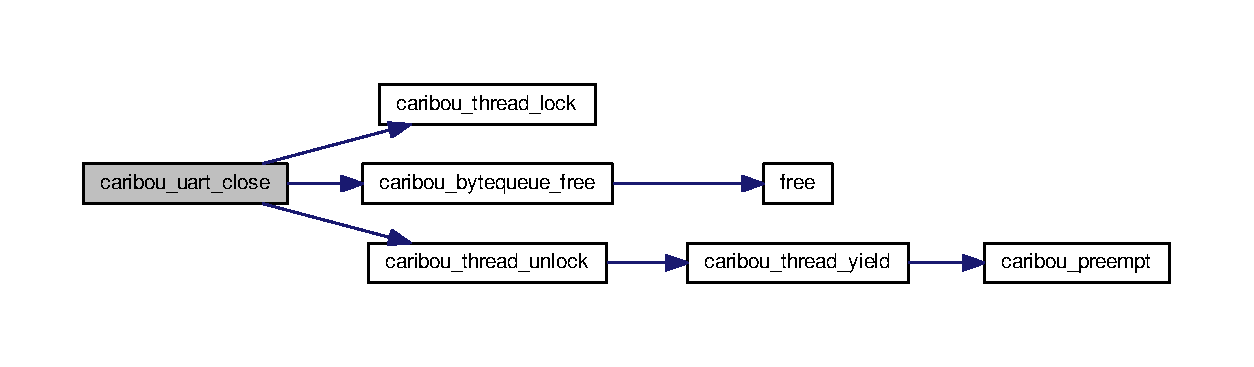
\includegraphics[width=350pt]{uart_8h_a69c58ec3847a900168737c43dec3fcbc_cgraph}
\end{center}
\end{figure}




Here is the caller graph for this function\-:
\nopagebreak
\begin{figure}[H]
\begin{center}
\leavevmode
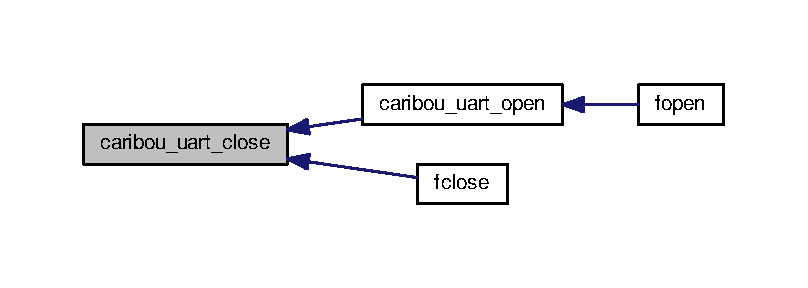
\includegraphics[width=350pt]{uart_8h_a69c58ec3847a900168737c43dec3fcbc_icgraph}
\end{center}
\end{figure}


\hypertarget{uart_8h_a52579b7ba4ba9c9b36f770e12d26de65}{\index{uart.\-h@{uart.\-h}!caribou\-\_\-uart\-\_\-disable@{caribou\-\_\-uart\-\_\-disable}}
\index{caribou\-\_\-uart\-\_\-disable@{caribou\-\_\-uart\-\_\-disable}!uart.h@{uart.\-h}}
\subsubsection[{caribou\-\_\-uart\-\_\-disable}]{\setlength{\rightskip}{0pt plus 5cm}void caribou\-\_\-uart\-\_\-disable (
\begin{DoxyParamCaption}
\item[{int}]{fd}
\end{DoxyParamCaption}
)}}\label{uart_8h_a52579b7ba4ba9c9b36f770e12d26de65}


Definition at line 257 of file uart.\-c.



Here is the call graph for this function\-:
\nopagebreak
\begin{figure}[H]
\begin{center}
\leavevmode
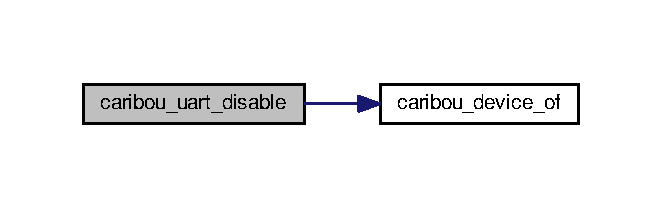
\includegraphics[width=318pt]{uart_8h_a52579b7ba4ba9c9b36f770e12d26de65_cgraph}
\end{center}
\end{figure}


\hypertarget{uart_8h_ac60f61b823d817b68cf858a7404980ea}{\index{uart.\-h@{uart.\-h}!caribou\-\_\-uart\-\_\-enable@{caribou\-\_\-uart\-\_\-enable}}
\index{caribou\-\_\-uart\-\_\-enable@{caribou\-\_\-uart\-\_\-enable}!uart.h@{uart.\-h}}
\subsubsection[{caribou\-\_\-uart\-\_\-enable}]{\setlength{\rightskip}{0pt plus 5cm}void caribou\-\_\-uart\-\_\-enable (
\begin{DoxyParamCaption}
\item[{int}]{fd}
\end{DoxyParamCaption}
)}}\label{uart_8h_ac60f61b823d817b68cf858a7404980ea}


Definition at line 252 of file uart.\-c.



Here is the call graph for this function\-:
\nopagebreak
\begin{figure}[H]
\begin{center}
\leavevmode
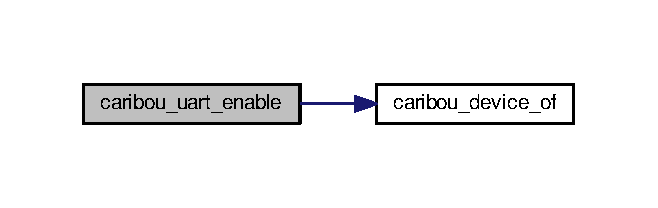
\includegraphics[width=316pt]{uart_8h_ac60f61b823d817b68cf858a7404980ea_cgraph}
\end{center}
\end{figure}


\hypertarget{uart_8h_a93b1a50c466b5579ee6080cd378114b6}{\index{uart.\-h@{uart.\-h}!caribou\-\_\-uart\-\_\-init\-\_\-config@{caribou\-\_\-uart\-\_\-init\-\_\-config}}
\index{caribou\-\_\-uart\-\_\-init\-\_\-config@{caribou\-\_\-uart\-\_\-init\-\_\-config}!uart.h@{uart.\-h}}
\subsubsection[{caribou\-\_\-uart\-\_\-init\-\_\-config}]{\setlength{\rightskip}{0pt plus 5cm}void caribou\-\_\-uart\-\_\-init\-\_\-config (
\begin{DoxyParamCaption}
\item[{{\bf caribou\-\_\-uart\-\_\-config\-\_\-t} $\ast$}]{config}
\end{DoxyParamCaption}
)}}\label{uart_8h_a93b1a50c466b5579ee6080cd378114b6}


Initialize the config record to contain sane values. 



Definition at line 117 of file uart.\-c.



Here is the call graph for this function\-:
\nopagebreak
\begin{figure}[H]
\begin{center}
\leavevmode
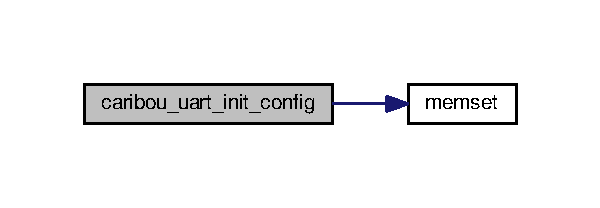
\includegraphics[width=288pt]{uart_8h_a93b1a50c466b5579ee6080cd378114b6_cgraph}
\end{center}
\end{figure}


\hypertarget{uart_8h_a5fb29fdb37419d5e8f37beafe6075322}{\index{uart.\-h@{uart.\-h}!caribou\-\_\-uart\-\_\-int\-\_\-disable@{caribou\-\_\-uart\-\_\-int\-\_\-disable}}
\index{caribou\-\_\-uart\-\_\-int\-\_\-disable@{caribou\-\_\-uart\-\_\-int\-\_\-disable}!uart.h@{uart.\-h}}
\subsubsection[{caribou\-\_\-uart\-\_\-int\-\_\-disable}]{\setlength{\rightskip}{0pt plus 5cm}int caribou\-\_\-uart\-\_\-int\-\_\-disable (
\begin{DoxyParamCaption}
\item[{int}]{fd}
\end{DoxyParamCaption}
)}}\label{uart_8h_a5fb29fdb37419d5e8f37beafe6075322}


Disable U\-A\-R\-T interrupts. 


\begin{DoxyParams}{Parameters}
{\em fd} & The open U\-A\-R\-T file descriptor. \\
\hline
\end{DoxyParams}
\begin{DoxyReturn}{Returns}
The previous interrupt state. 
\end{DoxyReturn}


Definition at line 183 of file uart.\-c.



Here is the call graph for this function\-:
\nopagebreak
\begin{figure}[H]
\begin{center}
\leavevmode
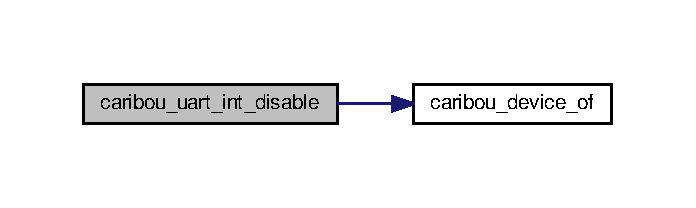
\includegraphics[width=334pt]{uart_8h_a5fb29fdb37419d5e8f37beafe6075322_cgraph}
\end{center}
\end{figure}


\hypertarget{uart_8h_a64d85da5442a9faeeae387fc7f971412}{\index{uart.\-h@{uart.\-h}!caribou\-\_\-uart\-\_\-int\-\_\-enable@{caribou\-\_\-uart\-\_\-int\-\_\-enable}}
\index{caribou\-\_\-uart\-\_\-int\-\_\-enable@{caribou\-\_\-uart\-\_\-int\-\_\-enable}!uart.h@{uart.\-h}}
\subsubsection[{caribou\-\_\-uart\-\_\-int\-\_\-enable}]{\setlength{\rightskip}{0pt plus 5cm}int caribou\-\_\-uart\-\_\-int\-\_\-enable (
\begin{DoxyParamCaption}
\item[{int}]{fd}
\end{DoxyParamCaption}
)}}\label{uart_8h_a64d85da5442a9faeeae387fc7f971412}


Enable U\-A\-R\-T interrupts. 


\begin{DoxyParams}{Parameters}
{\em fd} & The open U\-A\-R\-T file descriptor. \\
\hline
\end{DoxyParams}
\begin{DoxyReturn}{Returns}
The previous interrupt state. 
\end{DoxyReturn}


Definition at line 172 of file uart.\-c.



Here is the call graph for this function\-:
\nopagebreak
\begin{figure}[H]
\begin{center}
\leavevmode
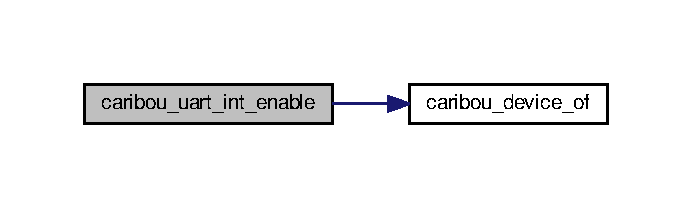
\includegraphics[width=332pt]{uart_8h_a64d85da5442a9faeeae387fc7f971412_cgraph}
\end{center}
\end{figure}


\hypertarget{uart_8h_a6a4f7e52bda927444a0b0fa1af205651}{\index{uart.\-h@{uart.\-h}!caribou\-\_\-uart\-\_\-int\-\_\-enabled@{caribou\-\_\-uart\-\_\-int\-\_\-enabled}}
\index{caribou\-\_\-uart\-\_\-int\-\_\-enabled@{caribou\-\_\-uart\-\_\-int\-\_\-enabled}!uart.h@{uart.\-h}}
\subsubsection[{caribou\-\_\-uart\-\_\-int\-\_\-enabled}]{\setlength{\rightskip}{0pt plus 5cm}int caribou\-\_\-uart\-\_\-int\-\_\-enabled (
\begin{DoxyParamCaption}
\item[{int}]{fd}
\end{DoxyParamCaption}
)}}\label{uart_8h_a6a4f7e52bda927444a0b0fa1af205651}


Determine if the U\-A\-R\-T interrupts are enabled. 


\begin{DoxyParams}{Parameters}
{\em fd} & The open U\-A\-R\-T file descriptor. \\
\hline
\end{DoxyParams}
\begin{DoxyReturn}{Returns}
The current interrupt state. 
\end{DoxyReturn}


Definition at line 194 of file uart.\-c.



Here is the call graph for this function\-:
\nopagebreak
\begin{figure}[H]
\begin{center}
\leavevmode
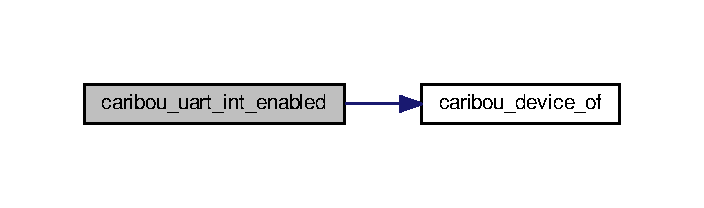
\includegraphics[width=338pt]{uart_8h_a6a4f7e52bda927444a0b0fa1af205651_cgraph}
\end{center}
\end{figure}


\hypertarget{uart_8h_a022166fd5acba50d49188e433eca93e0}{\index{uart.\-h@{uart.\-h}!caribou\-\_\-uart\-\_\-int\-\_\-set@{caribou\-\_\-uart\-\_\-int\-\_\-set}}
\index{caribou\-\_\-uart\-\_\-int\-\_\-set@{caribou\-\_\-uart\-\_\-int\-\_\-set}!uart.h@{uart.\-h}}
\subsubsection[{caribou\-\_\-uart\-\_\-int\-\_\-set}]{\setlength{\rightskip}{0pt plus 5cm}int caribou\-\_\-uart\-\_\-int\-\_\-set (
\begin{DoxyParamCaption}
\item[{int}]{fd, }
\item[{int}]{state}
\end{DoxyParamCaption}
)}}\label{uart_8h_a022166fd5acba50d49188e433eca93e0}


Set the U\-A\-R\-T interrupt state. 


\begin{DoxyParams}{Parameters}
{\em fd} & The U\-A\-R\-T file descriptor. \\
\hline
\end{DoxyParams}
\begin{DoxyReturn}{Returns}
void 
\end{DoxyReturn}


Definition at line 205 of file uart.\-c.



Here is the call graph for this function\-:
\nopagebreak
\begin{figure}[H]
\begin{center}
\leavevmode
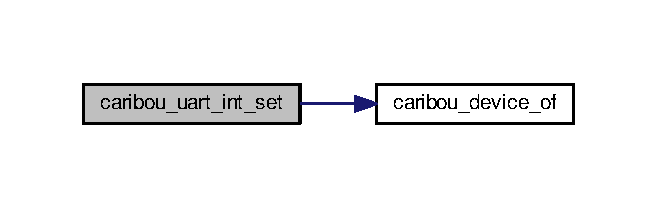
\includegraphics[width=316pt]{uart_8h_a022166fd5acba50d49188e433eca93e0_cgraph}
\end{center}
\end{figure}


\hypertarget{uart_8h_a9a85b0c56dbc7199c9608979903272ab}{\index{uart.\-h@{uart.\-h}!caribou\-\_\-uart\-\_\-open@{caribou\-\_\-uart\-\_\-open}}
\index{caribou\-\_\-uart\-\_\-open@{caribou\-\_\-uart\-\_\-open}!uart.h@{uart.\-h}}
\subsubsection[{caribou\-\_\-uart\-\_\-open}]{\setlength{\rightskip}{0pt plus 5cm}int caribou\-\_\-uart\-\_\-open (
\begin{DoxyParamCaption}
\item[{int}]{ndev, }
\item[{{\bf caribou\-\_\-uart\-\_\-config\-\_\-t} $\ast$}]{config}
\end{DoxyParamCaption}
)}}\label{uart_8h_a9a85b0c56dbc7199c9608979903272ab}


Open a U\-A\-R\-T device for subsequent use. 


\begin{DoxyParams}{Parameters}
{\em devicenum} & Specifies the device number to use. \\
\hline
\end{DoxyParams}
\begin{DoxyReturn}{Returns}
The file descriptor or $<$ 0 on error. 
\end{DoxyReturn}


Definition at line 44 of file uart.\-c.



Here is the call graph for this function\-:
\nopagebreak
\begin{figure}[H]
\begin{center}
\leavevmode
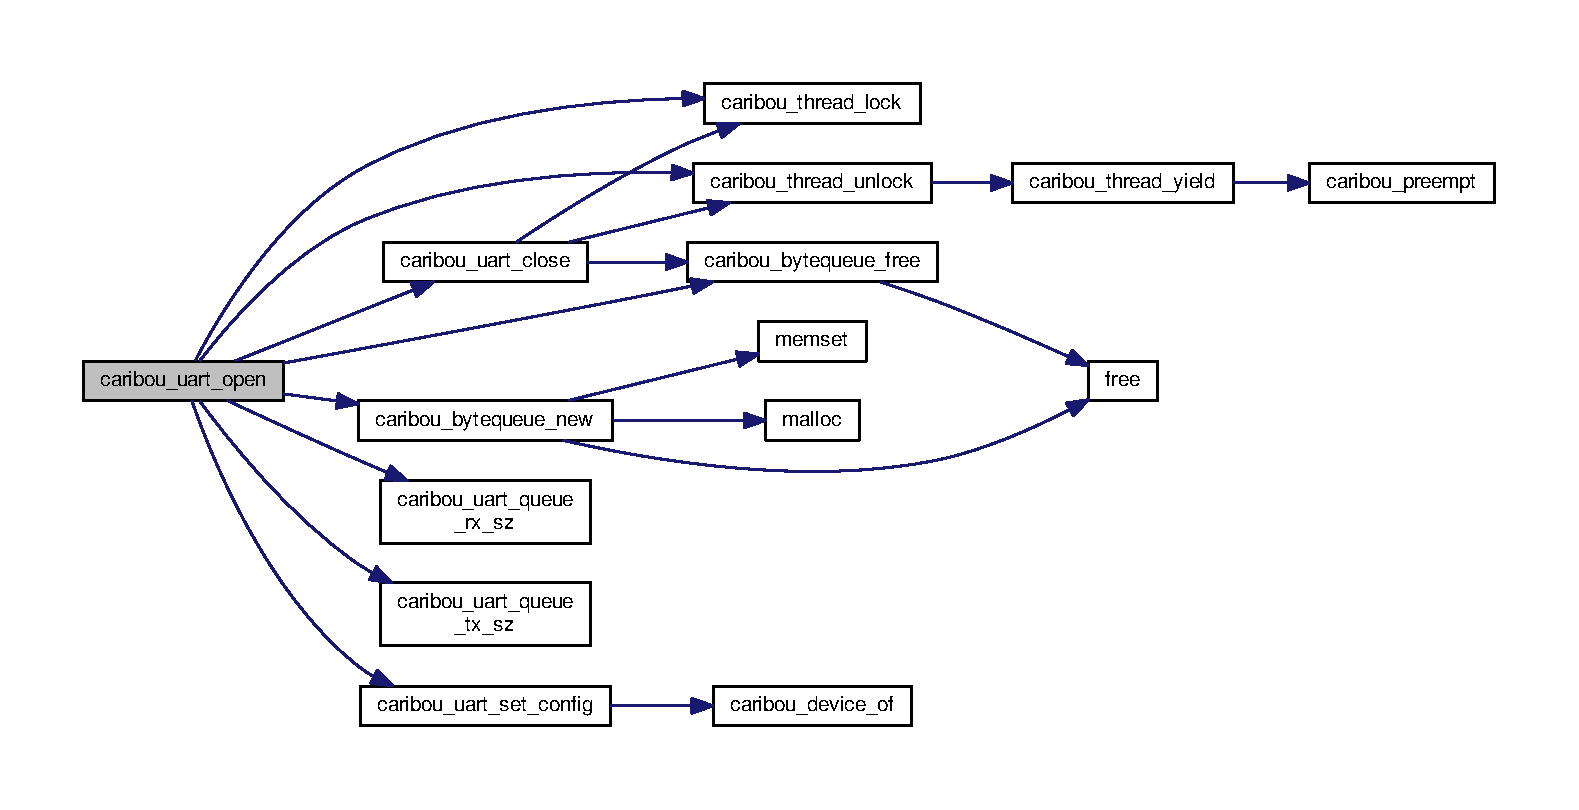
\includegraphics[width=350pt]{uart_8h_a9a85b0c56dbc7199c9608979903272ab_cgraph}
\end{center}
\end{figure}




Here is the caller graph for this function\-:
\nopagebreak
\begin{figure}[H]
\begin{center}
\leavevmode
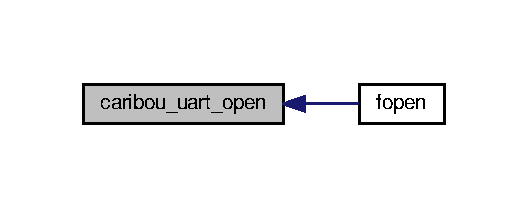
\includegraphics[width=254pt]{uart_8h_a9a85b0c56dbc7199c9608979903272ab_icgraph}
\end{center}
\end{figure}


\hypertarget{uart_8h_afaed2785671eb5acc7df6c3efe1c1515}{\index{uart.\-h@{uart.\-h}!caribou\-\_\-uart\-\_\-private\-\_\-readfn@{caribou\-\_\-uart\-\_\-private\-\_\-readfn}}
\index{caribou\-\_\-uart\-\_\-private\-\_\-readfn@{caribou\-\_\-uart\-\_\-private\-\_\-readfn}!uart.h@{uart.\-h}}
\subsubsection[{caribou\-\_\-uart\-\_\-private\-\_\-readfn}]{\setlength{\rightskip}{0pt plus 5cm}int caribou\-\_\-uart\-\_\-private\-\_\-readfn (
\begin{DoxyParamCaption}
\item[{{\bf stdio\-\_\-t} $\ast$}]{io, }
\item[{void $\ast$}]{data, }
\item[{int}]{count}
\end{DoxyParamCaption}
)}}\label{uart_8h_afaed2785671eb5acc7df6c3efe1c1515}


F\-I\-X\-M\-E make really private declarations. 

Device Driver read-\/data function. \begin{DoxyReturn}{Returns}
number of bytes read, or $<$ 0 + errno 
\end{DoxyReturn}


Definition at line 264 of file uart.\-c.



Here is the call graph for this function\-:
\nopagebreak
\begin{figure}[H]
\begin{center}
\leavevmode
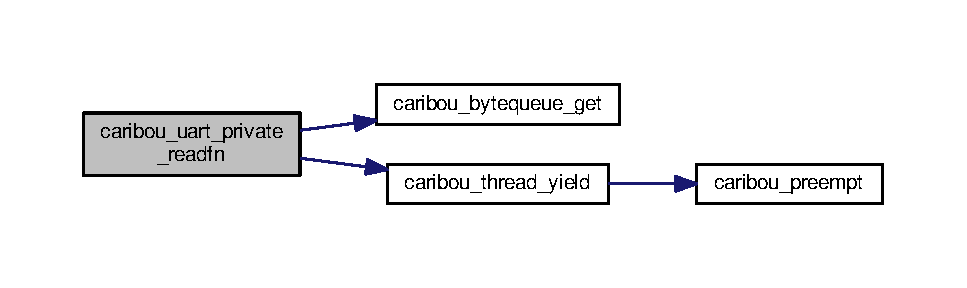
\includegraphics[width=350pt]{uart_8h_afaed2785671eb5acc7df6c3efe1c1515_cgraph}
\end{center}
\end{figure}


\hypertarget{uart_8h_a104d19d00c26c184eb6b352539b146a8}{\index{uart.\-h@{uart.\-h}!caribou\-\_\-uart\-\_\-private\-\_\-readqueuefn@{caribou\-\_\-uart\-\_\-private\-\_\-readqueuefn}}
\index{caribou\-\_\-uart\-\_\-private\-\_\-readqueuefn@{caribou\-\_\-uart\-\_\-private\-\_\-readqueuefn}!uart.h@{uart.\-h}}
\subsubsection[{caribou\-\_\-uart\-\_\-private\-\_\-readqueuefn}]{\setlength{\rightskip}{0pt plus 5cm}int caribou\-\_\-uart\-\_\-private\-\_\-readqueuefn (
\begin{DoxyParamCaption}
\item[{{\bf stdio\-\_\-t} $\ast$}]{io}
\end{DoxyParamCaption}
)}}\label{uart_8h_a104d19d00c26c184eb6b352539b146a8}


Device Driver write-\/data function. 

Device Driver write-\/data function. 

Definition at line 308 of file uart.\-c.



Here is the call graph for this function\-:
\nopagebreak
\begin{figure}[H]
\begin{center}
\leavevmode
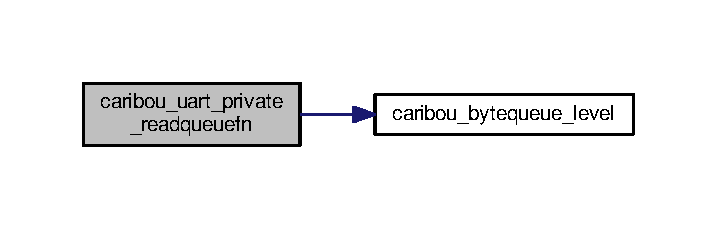
\includegraphics[width=344pt]{uart_8h_a104d19d00c26c184eb6b352539b146a8_cgraph}
\end{center}
\end{figure}


\hypertarget{uart_8h_ad888daa7223dda1848704a8ddf83df5d}{\index{uart.\-h@{uart.\-h}!caribou\-\_\-uart\-\_\-private\-\_\-statefn@{caribou\-\_\-uart\-\_\-private\-\_\-statefn}}
\index{caribou\-\_\-uart\-\_\-private\-\_\-statefn@{caribou\-\_\-uart\-\_\-private\-\_\-statefn}!uart.h@{uart.\-h}}
\subsubsection[{caribou\-\_\-uart\-\_\-private\-\_\-statefn}]{\setlength{\rightskip}{0pt plus 5cm}int caribou\-\_\-uart\-\_\-private\-\_\-statefn (
\begin{DoxyParamCaption}
\item[{{\bf stdio\-\_\-t} $\ast$}]{io}
\end{DoxyParamCaption}
)}}\label{uart_8h_ad888daa7223dda1848704a8ddf83df5d}


Device Driver write-\/data pending. 

Device Driver write-\/data pending. 

Definition at line 320 of file uart.\-c.

\hypertarget{uart_8h_a5f7ddc5c012cb9967d9053f3b5b3c8a3}{\index{uart.\-h@{uart.\-h}!caribou\-\_\-uart\-\_\-private\-\_\-writefn@{caribou\-\_\-uart\-\_\-private\-\_\-writefn}}
\index{caribou\-\_\-uart\-\_\-private\-\_\-writefn@{caribou\-\_\-uart\-\_\-private\-\_\-writefn}!uart.h@{uart.\-h}}
\subsubsection[{caribou\-\_\-uart\-\_\-private\-\_\-writefn}]{\setlength{\rightskip}{0pt plus 5cm}int caribou\-\_\-uart\-\_\-private\-\_\-writefn (
\begin{DoxyParamCaption}
\item[{{\bf stdio\-\_\-t} $\ast$}]{io, }
\item[{void $\ast$}]{data, }
\item[{int}]{count}
\end{DoxyParamCaption}
)}}\label{uart_8h_a5f7ddc5c012cb9967d9053f3b5b3c8a3}


Device Driver read-\/data function. 

Device Driver read-\/data function. 

Definition at line 285 of file uart.\-c.



Here is the call graph for this function\-:
\nopagebreak
\begin{figure}[H]
\begin{center}
\leavevmode
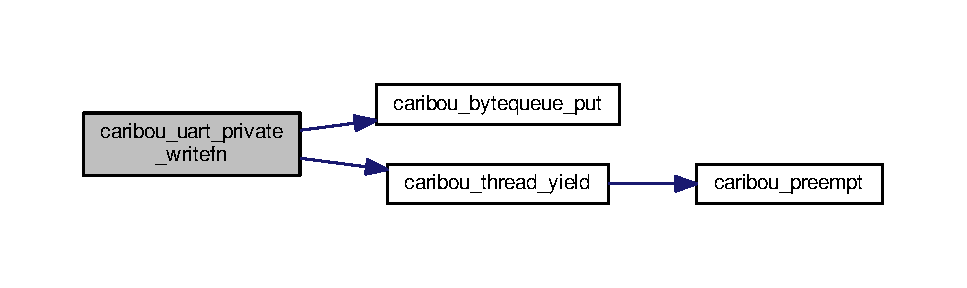
\includegraphics[width=350pt]{uart_8h_a5f7ddc5c012cb9967d9053f3b5b3c8a3_cgraph}
\end{center}
\end{figure}


\hypertarget{uart_8h_a133b9c5413db93d9d99fefc550dbd2ab}{\index{uart.\-h@{uart.\-h}!caribou\-\_\-uart\-\_\-private\-\_\-writequeuefn@{caribou\-\_\-uart\-\_\-private\-\_\-writequeuefn}}
\index{caribou\-\_\-uart\-\_\-private\-\_\-writequeuefn@{caribou\-\_\-uart\-\_\-private\-\_\-writequeuefn}!uart.h@{uart.\-h}}
\subsubsection[{caribou\-\_\-uart\-\_\-private\-\_\-writequeuefn}]{\setlength{\rightskip}{0pt plus 5cm}int caribou\-\_\-uart\-\_\-private\-\_\-writequeuefn (
\begin{DoxyParamCaption}
\item[{{\bf stdio\-\_\-t} $\ast$}]{io}
\end{DoxyParamCaption}
)}}\label{uart_8h_a133b9c5413db93d9d99fefc550dbd2ab}


Device Driver read-\/data available function. 

Device Driver read-\/data available function. 

Definition at line 314 of file uart.\-c.



Here is the call graph for this function\-:
\nopagebreak
\begin{figure}[H]
\begin{center}
\leavevmode
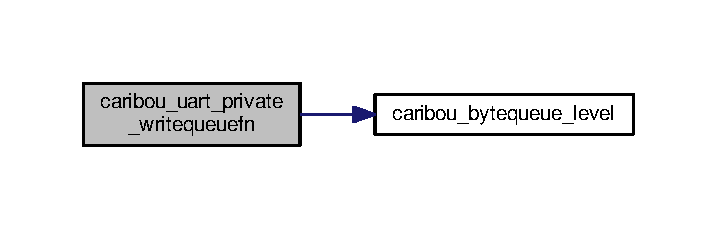
\includegraphics[width=344pt]{uart_8h_a133b9c5413db93d9d99fefc550dbd2ab_cgraph}
\end{center}
\end{figure}


\hypertarget{uart_8h_a351e35bbfed47860d7f40fb1fba387be}{\index{uart.\-h@{uart.\-h}!caribou\-\_\-uart\-\_\-queue\-\_\-rx\-\_\-sz@{caribou\-\_\-uart\-\_\-queue\-\_\-rx\-\_\-sz}}
\index{caribou\-\_\-uart\-\_\-queue\-\_\-rx\-\_\-sz@{caribou\-\_\-uart\-\_\-queue\-\_\-rx\-\_\-sz}!uart.h@{uart.\-h}}
\subsubsection[{caribou\-\_\-uart\-\_\-queue\-\_\-rx\-\_\-sz}]{\setlength{\rightskip}{0pt plus 5cm}int caribou\-\_\-uart\-\_\-queue\-\_\-rx\-\_\-sz (
\begin{DoxyParamCaption}
{}
\end{DoxyParamCaption}
)}}\label{uart_8h_a351e35bbfed47860d7f40fb1fba387be}
\begin{DoxyReturn}{Returns}
The standard receiver queue size in bytes. 
\end{DoxyReturn}


Definition at line 152 of file uart.\-c.



Here is the caller graph for this function\-:
\nopagebreak
\begin{figure}[H]
\begin{center}
\leavevmode
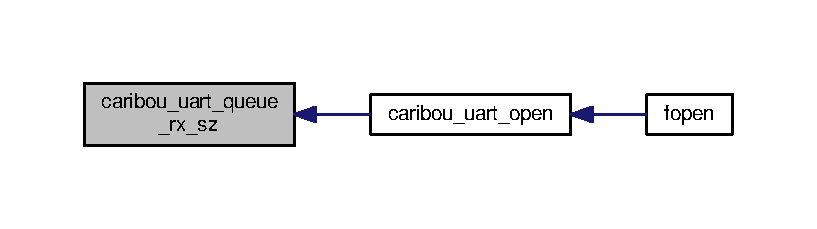
\includegraphics[width=350pt]{uart_8h_a351e35bbfed47860d7f40fb1fba387be_icgraph}
\end{center}
\end{figure}


\hypertarget{uart_8h_a297914e4527fd034ffbf95c740d2f37f}{\index{uart.\-h@{uart.\-h}!caribou\-\_\-uart\-\_\-queue\-\_\-tx\-\_\-sz@{caribou\-\_\-uart\-\_\-queue\-\_\-tx\-\_\-sz}}
\index{caribou\-\_\-uart\-\_\-queue\-\_\-tx\-\_\-sz@{caribou\-\_\-uart\-\_\-queue\-\_\-tx\-\_\-sz}!uart.h@{uart.\-h}}
\subsubsection[{caribou\-\_\-uart\-\_\-queue\-\_\-tx\-\_\-sz}]{\setlength{\rightskip}{0pt plus 5cm}int caribou\-\_\-uart\-\_\-queue\-\_\-tx\-\_\-sz (
\begin{DoxyParamCaption}
{}
\end{DoxyParamCaption}
)}}\label{uart_8h_a297914e4527fd034ffbf95c740d2f37f}
\begin{DoxyReturn}{Returns}
The standard transmitter queue size in bytes. 
\end{DoxyReturn}


Definition at line 144 of file uart.\-c.



Here is the caller graph for this function\-:
\nopagebreak
\begin{figure}[H]
\begin{center}
\leavevmode
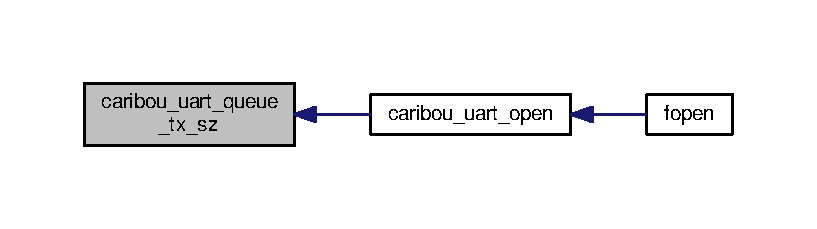
\includegraphics[width=350pt]{uart_8h_a297914e4527fd034ffbf95c740d2f37f_icgraph}
\end{center}
\end{figure}


\hypertarget{uart_8h_a0a8cbc25e619395ae7c4de7895da3a41}{\index{uart.\-h@{uart.\-h}!caribou\-\_\-uart\-\_\-rx\-\_\-data@{caribou\-\_\-uart\-\_\-rx\-\_\-data}}
\index{caribou\-\_\-uart\-\_\-rx\-\_\-data@{caribou\-\_\-uart\-\_\-rx\-\_\-data}!uart.h@{uart.\-h}}
\subsubsection[{caribou\-\_\-uart\-\_\-rx\-\_\-data}]{\setlength{\rightskip}{0pt plus 5cm}int caribou\-\_\-uart\-\_\-rx\-\_\-data (
\begin{DoxyParamCaption}
\item[{int}]{fd}
\end{DoxyParamCaption}
)}}\label{uart_8h_a0a8cbc25e619395ae7c4de7895da3a41}


Retrieve a byte from the U\-A\-R\-T holding register. 



Definition at line 223 of file uart.\-c.



Here is the call graph for this function\-:
\nopagebreak
\begin{figure}[H]
\begin{center}
\leavevmode
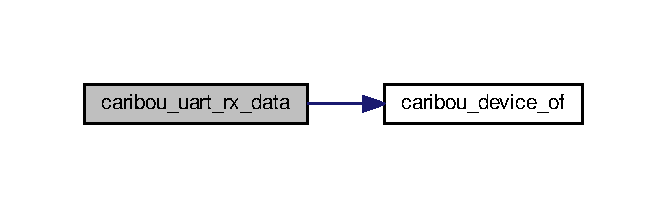
\includegraphics[width=320pt]{uart_8h_a0a8cbc25e619395ae7c4de7895da3a41_cgraph}
\end{center}
\end{figure}


\hypertarget{uart_8h_a8b7d4543a230f68ca97188aa64da2ad1}{\index{uart.\-h@{uart.\-h}!caribou\-\_\-uart\-\_\-rx\-\_\-queue@{caribou\-\_\-uart\-\_\-rx\-\_\-queue}}
\index{caribou\-\_\-uart\-\_\-rx\-\_\-queue@{caribou\-\_\-uart\-\_\-rx\-\_\-queue}!uart.h@{uart.\-h}}
\subsubsection[{caribou\-\_\-uart\-\_\-rx\-\_\-queue}]{\setlength{\rightskip}{0pt plus 5cm}{\bf caribou\-\_\-bytequeue\-\_\-t}$\ast$ caribou\-\_\-uart\-\_\-rx\-\_\-queue (
\begin{DoxyParamCaption}
\item[{int}]{fd}
\end{DoxyParamCaption}
)}}\label{uart_8h_a8b7d4543a230f68ca97188aa64da2ad1}


Definition at line 157 of file uart.\-c.



Here is the call graph for this function\-:
\nopagebreak
\begin{figure}[H]
\begin{center}
\leavevmode
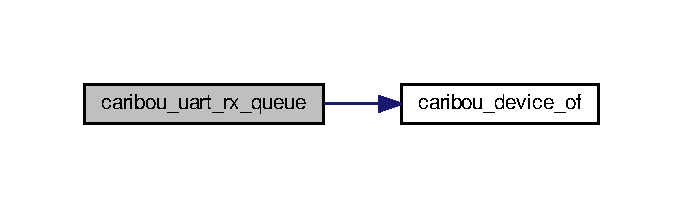
\includegraphics[width=328pt]{uart_8h_a8b7d4543a230f68ca97188aa64da2ad1_cgraph}
\end{center}
\end{figure}


\hypertarget{uart_8h_aa82184396ed62090414e5bd4f3d3ab0c}{\index{uart.\-h@{uart.\-h}!caribou\-\_\-uart\-\_\-rx\-\_\-ready@{caribou\-\_\-uart\-\_\-rx\-\_\-ready}}
\index{caribou\-\_\-uart\-\_\-rx\-\_\-ready@{caribou\-\_\-uart\-\_\-rx\-\_\-ready}!uart.h@{uart.\-h}}
\subsubsection[{caribou\-\_\-uart\-\_\-rx\-\_\-ready}]{\setlength{\rightskip}{0pt plus 5cm}{\bf bool} caribou\-\_\-uart\-\_\-rx\-\_\-ready (
\begin{DoxyParamCaption}
\item[{int}]{fd}
\end{DoxyParamCaption}
)}}\label{uart_8h_aa82184396ed62090414e5bd4f3d3ab0c}


Determine of receiver has data ready. 



Definition at line 247 of file uart.\-c.



Here is the call graph for this function\-:
\nopagebreak
\begin{figure}[H]
\begin{center}
\leavevmode
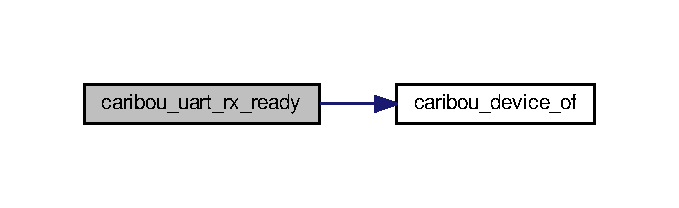
\includegraphics[width=326pt]{uart_8h_aa82184396ed62090414e5bd4f3d3ab0c_cgraph}
\end{center}
\end{figure}


\hypertarget{uart_8h_a95be81c80a3d8d897177069628a7b18f}{\index{uart.\-h@{uart.\-h}!caribou\-\_\-uart\-\_\-set\-\_\-config@{caribou\-\_\-uart\-\_\-set\-\_\-config}}
\index{caribou\-\_\-uart\-\_\-set\-\_\-config@{caribou\-\_\-uart\-\_\-set\-\_\-config}!uart.h@{uart.\-h}}
\subsubsection[{caribou\-\_\-uart\-\_\-set\-\_\-config}]{\setlength{\rightskip}{0pt plus 5cm}int caribou\-\_\-uart\-\_\-set\-\_\-config (
\begin{DoxyParamCaption}
\item[{int}]{fd, }
\item[{{\bf caribou\-\_\-uart\-\_\-config\-\_\-t} $\ast$}]{config}
\end{DoxyParamCaption}
)}}\label{uart_8h_a95be81c80a3d8d897177069628a7b18f}


Set the U\-A\-R\-T configuration. 


\begin{DoxyParams}{Parameters}
{\em fd} & The opened U\-A\-R\-T file descriptor. \\
\hline
\end{DoxyParams}
\begin{DoxyReturn}{Returns}
$<$ 0 on error. 
\end{DoxyReturn}


Definition at line 135 of file uart.\-c.



Here is the call graph for this function\-:
\nopagebreak
\begin{figure}[H]
\begin{center}
\leavevmode
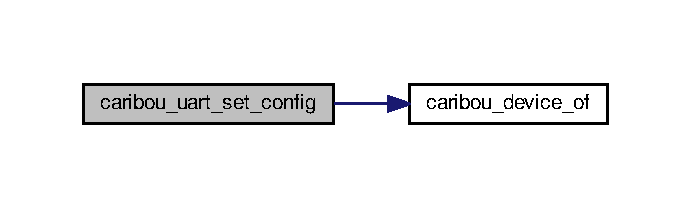
\includegraphics[width=332pt]{uart_8h_a95be81c80a3d8d897177069628a7b18f_cgraph}
\end{center}
\end{figure}




Here is the caller graph for this function\-:
\nopagebreak
\begin{figure}[H]
\begin{center}
\leavevmode
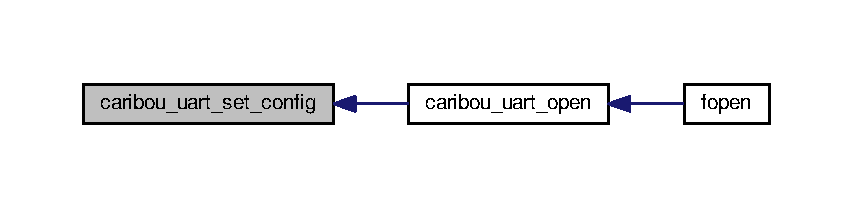
\includegraphics[width=350pt]{uart_8h_a95be81c80a3d8d897177069628a7b18f_icgraph}
\end{center}
\end{figure}


\hypertarget{uart_8h_ac598aa7ccb4824abe80296502d27ec86}{\index{uart.\-h@{uart.\-h}!caribou\-\_\-uart\-\_\-tx\-\_\-busy@{caribou\-\_\-uart\-\_\-tx\-\_\-busy}}
\index{caribou\-\_\-uart\-\_\-tx\-\_\-busy@{caribou\-\_\-uart\-\_\-tx\-\_\-busy}!uart.h@{uart.\-h}}
\subsubsection[{caribou\-\_\-uart\-\_\-tx\-\_\-busy}]{\setlength{\rightskip}{0pt plus 5cm}{\bf bool} caribou\-\_\-uart\-\_\-tx\-\_\-busy (
\begin{DoxyParamCaption}
\item[{int}]{fd}
\end{DoxyParamCaption}
)}}\label{uart_8h_ac598aa7ccb4824abe80296502d27ec86}


Determine of the U\-A\-R\-T transmitter is busy. 



Definition at line 231 of file uart.\-c.



Here is the call graph for this function\-:
\nopagebreak
\begin{figure}[H]
\begin{center}
\leavevmode
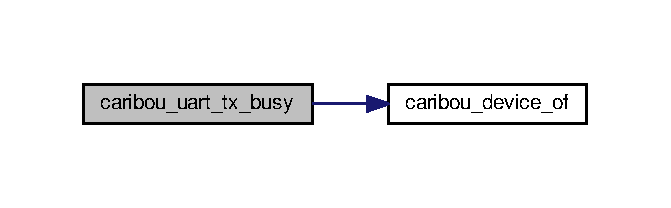
\includegraphics[width=322pt]{uart_8h_ac598aa7ccb4824abe80296502d27ec86_cgraph}
\end{center}
\end{figure}


\hypertarget{uart_8h_ad763845504097b6d6debe7ec52f60fb3}{\index{uart.\-h@{uart.\-h}!caribou\-\_\-uart\-\_\-tx\-\_\-data@{caribou\-\_\-uart\-\_\-tx\-\_\-data}}
\index{caribou\-\_\-uart\-\_\-tx\-\_\-data@{caribou\-\_\-uart\-\_\-tx\-\_\-data}!uart.h@{uart.\-h}}
\subsubsection[{caribou\-\_\-uart\-\_\-tx\-\_\-data}]{\setlength{\rightskip}{0pt plus 5cm}int caribou\-\_\-uart\-\_\-tx\-\_\-data (
\begin{DoxyParamCaption}
\item[{int}]{fd, }
\item[{int}]{ch}
\end{DoxyParamCaption}
)}}\label{uart_8h_ad763845504097b6d6debe7ec52f60fb3}


Place a byte into the U\-A\-R\-T transmit buffer. 

\begin{DoxyReturn}{Returns}
the byte., 
\end{DoxyReturn}


Definition at line 215 of file uart.\-c.



Here is the call graph for this function\-:
\nopagebreak
\begin{figure}[H]
\begin{center}
\leavevmode
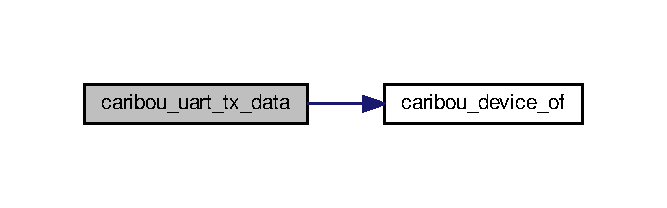
\includegraphics[width=320pt]{uart_8h_ad763845504097b6d6debe7ec52f60fb3_cgraph}
\end{center}
\end{figure}


\hypertarget{uart_8h_a6b2993300e7c152eb6cc992feaf98c9a}{\index{uart.\-h@{uart.\-h}!caribou\-\_\-uart\-\_\-tx\-\_\-queue@{caribou\-\_\-uart\-\_\-tx\-\_\-queue}}
\index{caribou\-\_\-uart\-\_\-tx\-\_\-queue@{caribou\-\_\-uart\-\_\-tx\-\_\-queue}!uart.h@{uart.\-h}}
\subsubsection[{caribou\-\_\-uart\-\_\-tx\-\_\-queue}]{\setlength{\rightskip}{0pt plus 5cm}{\bf caribou\-\_\-bytequeue\-\_\-t}$\ast$ caribou\-\_\-uart\-\_\-tx\-\_\-queue (
\begin{DoxyParamCaption}
\item[{int}]{fd}
\end{DoxyParamCaption}
)}}\label{uart_8h_a6b2993300e7c152eb6cc992feaf98c9a}


Definition at line 162 of file uart.\-c.



Here is the call graph for this function\-:
\nopagebreak
\begin{figure}[H]
\begin{center}
\leavevmode
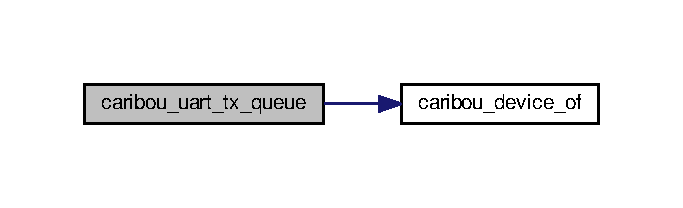
\includegraphics[width=328pt]{uart_8h_a6b2993300e7c152eb6cc992feaf98c9a_cgraph}
\end{center}
\end{figure}


\hypertarget{uart_8h_af3210bdc9cd62075c0143b639c581772}{\index{uart.\-h@{uart.\-h}!caribou\-\_\-uart\-\_\-tx\-\_\-ready@{caribou\-\_\-uart\-\_\-tx\-\_\-ready}}
\index{caribou\-\_\-uart\-\_\-tx\-\_\-ready@{caribou\-\_\-uart\-\_\-tx\-\_\-ready}!uart.h@{uart.\-h}}
\subsubsection[{caribou\-\_\-uart\-\_\-tx\-\_\-ready}]{\setlength{\rightskip}{0pt plus 5cm}{\bf bool} caribou\-\_\-uart\-\_\-tx\-\_\-ready (
\begin{DoxyParamCaption}
\item[{int}]{fd}
\end{DoxyParamCaption}
)}}\label{uart_8h_af3210bdc9cd62075c0143b639c581772}


Determine of the U\-A\-R\-T transmitter is ready to accept a byte. 



Definition at line 239 of file uart.\-c.



Here is the call graph for this function\-:
\nopagebreak
\begin{figure}[H]
\begin{center}
\leavevmode
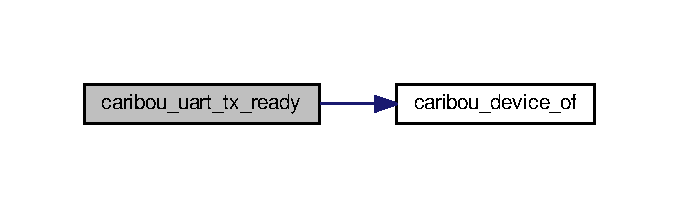
\includegraphics[width=326pt]{uart_8h_af3210bdc9cd62075c0143b639c581772_cgraph}
\end{center}
\end{figure}



\hypertarget{interrupt_8h}{\section{include/caribou/kernel/interrupt.h File Reference}
\label{interrupt_8h}\index{include/caribou/kernel/interrupt.\-h@{include/caribou/kernel/interrupt.\-h}}
}
{\ttfamily \#include $<$caribou/kernel/types.\-h$>$}\\*
{\ttfamily \#include $<$chip/chip.\-h$>$}\\*
Include dependency graph for interrupt.\-h\-:
\nopagebreak
\begin{figure}[H]
\begin{center}
\leavevmode
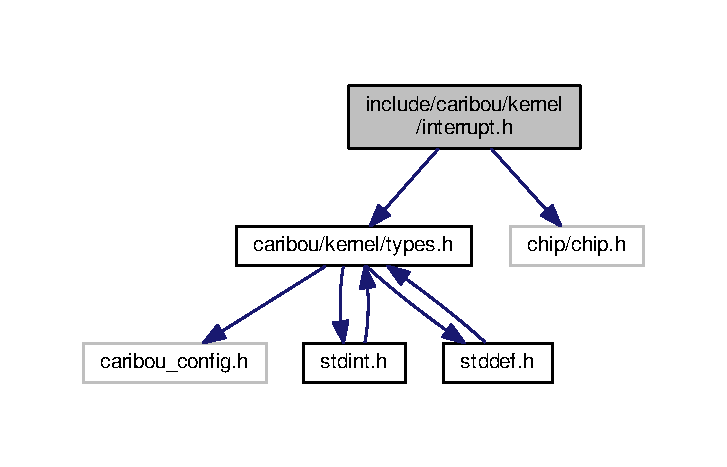
\includegraphics[width=349pt]{interrupt_8h__incl}
\end{center}
\end{figure}
This graph shows which files directly or indirectly include this file\-:
\nopagebreak
\begin{figure}[H]
\begin{center}
\leavevmode
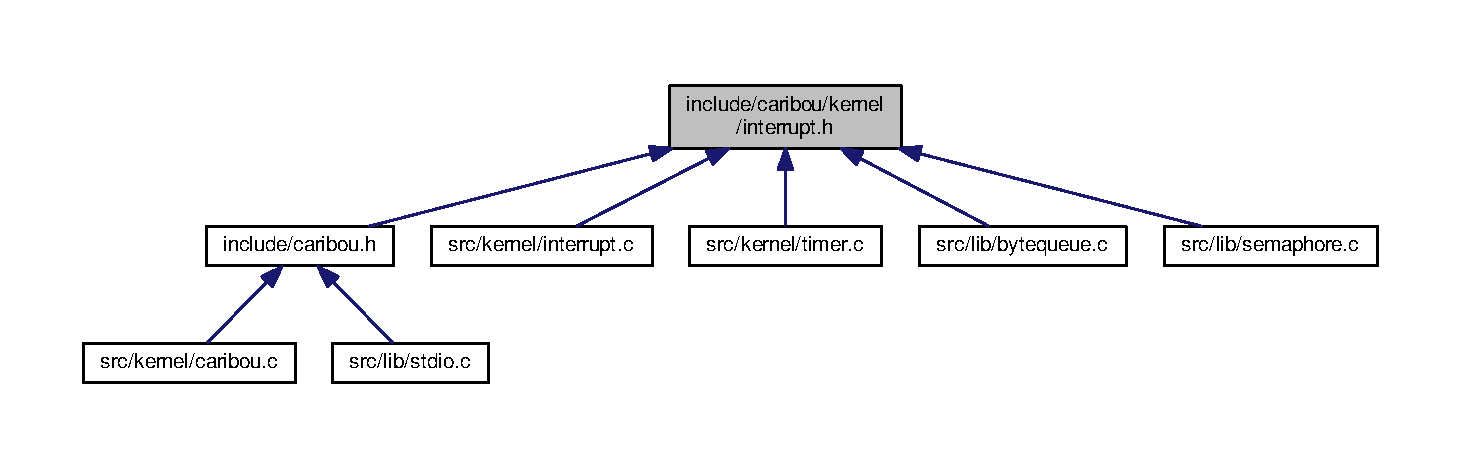
\includegraphics[width=350pt]{interrupt_8h__dep__incl}
\end{center}
\end{figure}
\subsection*{Macros}
\begin{DoxyCompactItemize}
\item 
\#define \hyperlink{interrupt_8h_a7e61ccc131c02ac007f3d4847383c736}{caribou\-\_\-wfi}()~chip\-\_\-wfi()
\item 
\#define \hyperlink{interrupt_8h_ae1c94738b236fe499580ae3c2eb20cda}{caribou\-\_\-interrupts\-\_\-enable}()~chip\-\_\-interrupts\-\_\-enable()
\item 
\#define \hyperlink{interrupt_8h_a803372faeae4e031dbee6565159c1d65}{caribou\-\_\-interrupts\-\_\-disable}()~chip\-\_\-interrupts\-\_\-disable()
\item 
\#define \hyperlink{interrupt_8h_ab78a9174a95d94c477b4e53484b0e6b2}{caribou\-\_\-interrupts\-\_\-enabled}()~chip\-\_\-interrupts\-\_\-enabled()
\item 
\#define \hyperlink{interrupt_8h_a899ab89cfa70bb3da17d6d45c1e7bce6}{caribou\-\_\-interrupts\-\_\-set}(enable)~chip\-\_\-interrupts\-\_\-set(enable)
\item 
\#define \hyperlink{interrupt_8h_a464eb81f4680c0f0bd6796a8da21ac86}{caribou\-\_\-interrupt\-\_\-level}()~chip\-\_\-interrupt\-\_\-level()
\item 
\#define \hyperlink{interrupt_8h_ac4280f2157daf0c7a8b42559c75f18b7}{caribou\-\_\-vector\-\_\-enabled}(vector)~chip\-\_\-vector\-\_\-enabled(vector)
\item 
\#define \hyperlink{interrupt_8h_a704371d60aa845579fd1c489a39b58d1}{caribou\-\_\-vector\-\_\-enable}(vector)~chip\-\_\-vector\-\_\-enable(vector)
\item 
\#define \hyperlink{interrupt_8h_a8f1fe14114236722183e8414d8413439}{caribou\-\_\-vector\-\_\-disable}(vector)~chip\-\_\-vector\-\_\-disable(vector)
\item 
\#define \hyperlink{interrupt_8h_a0dc04153e29a5bc2c292a3711282bf15}{caribou\-\_\-vector\-\_\-pending}(vector)~chip\-\_\-vector\-\_\-pending(vector)
\item 
\#define \hyperlink{interrupt_8h_a44a3cfdf9dbf2fe8e6be42deb1a0160c}{caribou\-\_\-vector\-\_\-pend}(vector)~chip\-\_\-vector\-\_\-pend(vector)
\item 
\#define \hyperlink{interrupt_8h_a7e3b9078d0e163fb06a1422d9d4690f3}{caribou\-\_\-vector\-\_\-unpend}(vector)~chip\-\_\-vector\-\_\-unpend(vector)
\end{DoxyCompactItemize}
\subsection*{Typedefs}
\begin{DoxyCompactItemize}
\item 
typedef void($\ast$ \hyperlink{interrupt_8h_af609f1916308a4ac8148b51cad03f620}{caribou\-\_\-isr\-\_\-t} )(Interrupt\-Vector, void $\ast$)
\end{DoxyCompactItemize}
\subsection*{Functions}
\begin{DoxyCompactItemize}
\item 
void \hyperlink{interrupt_8h_a6761fd317200918e7db518f96fa0a99f}{caribou\-\_\-interrupt\-\_\-service} (Interrupt\-Vector vector)
\begin{DoxyCompactList}\small\item\em User-\/land Interrupt Service Routine entry point. \end{DoxyCompactList}\item 
int \hyperlink{interrupt_8h_a8a407a6df21907345b1d77629693ed02}{caribou\-\_\-vector\-\_\-installed} (Interrupt\-Vector vector, \hyperlink{interrupt_8h_af609f1916308a4ac8148b51cad03f620}{caribou\-\_\-isr\-\_\-t} isr, void $\ast$arg)
\begin{DoxyCompactList}\small\item\em Determine if a vector is already installed. \end{DoxyCompactList}\item 
int \hyperlink{interrupt_8h_a4a1c34144794c0d656c0bf6462f5de45}{caribou\-\_\-vector\-\_\-install} (Interrupt\-Vector vector, \hyperlink{interrupt_8h_af609f1916308a4ac8148b51cad03f620}{caribou\-\_\-isr\-\_\-t} isr, void $\ast$arg)
\begin{DoxyCompactList}\small\item\em Install the vector into the isr\-\_\-map chain. \end{DoxyCompactList}\item 
int \hyperlink{interrupt_8h_a6638f6163ea849bf37e8347a1b0b18ef}{caribou\-\_\-vector\-\_\-remove} (Interrupt\-Vector vector, \hyperlink{interrupt_8h_af609f1916308a4ac8148b51cad03f620}{caribou\-\_\-isr\-\_\-t} isr)
\begin{DoxyCompactList}\small\item\em Install the vector into the isr\-\_\-map chain. \end{DoxyCompactList}\item 
int \hyperlink{interrupt_8h_ac84f7bf1366a9195f7a6a0692bb07711}{caribou\-\_\-vector\-\_\-remove\-\_\-all} (void $\ast$arg)
\begin{DoxyCompactList}\small\item\em Remove all vectors associated with arg. \end{DoxyCompactList}\end{DoxyCompactItemize}


\subsection{Macro Definition Documentation}
\hypertarget{interrupt_8h_a464eb81f4680c0f0bd6796a8da21ac86}{\index{interrupt.\-h@{interrupt.\-h}!caribou\-\_\-interrupt\-\_\-level@{caribou\-\_\-interrupt\-\_\-level}}
\index{caribou\-\_\-interrupt\-\_\-level@{caribou\-\_\-interrupt\-\_\-level}!interrupt.h@{interrupt.\-h}}
\subsubsection[{caribou\-\_\-interrupt\-\_\-level}]{\setlength{\rightskip}{0pt plus 5cm}\#define caribou\-\_\-interrupt\-\_\-level(
\begin{DoxyParamCaption}
{}
\end{DoxyParamCaption}
)~chip\-\_\-interrupt\-\_\-level()}}\label{interrupt_8h_a464eb81f4680c0f0bd6796a8da21ac86}


Definition at line 35 of file interrupt.\-h.

\hypertarget{interrupt_8h_a803372faeae4e031dbee6565159c1d65}{\index{interrupt.\-h@{interrupt.\-h}!caribou\-\_\-interrupts\-\_\-disable@{caribou\-\_\-interrupts\-\_\-disable}}
\index{caribou\-\_\-interrupts\-\_\-disable@{caribou\-\_\-interrupts\-\_\-disable}!interrupt.h@{interrupt.\-h}}
\subsubsection[{caribou\-\_\-interrupts\-\_\-disable}]{\setlength{\rightskip}{0pt plus 5cm}\#define caribou\-\_\-interrupts\-\_\-disable(
\begin{DoxyParamCaption}
{}
\end{DoxyParamCaption}
)~chip\-\_\-interrupts\-\_\-disable()}}\label{interrupt_8h_a803372faeae4e031dbee6565159c1d65}


Definition at line 32 of file interrupt.\-h.

\hypertarget{interrupt_8h_ae1c94738b236fe499580ae3c2eb20cda}{\index{interrupt.\-h@{interrupt.\-h}!caribou\-\_\-interrupts\-\_\-enable@{caribou\-\_\-interrupts\-\_\-enable}}
\index{caribou\-\_\-interrupts\-\_\-enable@{caribou\-\_\-interrupts\-\_\-enable}!interrupt.h@{interrupt.\-h}}
\subsubsection[{caribou\-\_\-interrupts\-\_\-enable}]{\setlength{\rightskip}{0pt plus 5cm}\#define caribou\-\_\-interrupts\-\_\-enable(
\begin{DoxyParamCaption}
{}
\end{DoxyParamCaption}
)~chip\-\_\-interrupts\-\_\-enable()}}\label{interrupt_8h_ae1c94738b236fe499580ae3c2eb20cda}


Definition at line 31 of file interrupt.\-h.

\hypertarget{interrupt_8h_ab78a9174a95d94c477b4e53484b0e6b2}{\index{interrupt.\-h@{interrupt.\-h}!caribou\-\_\-interrupts\-\_\-enabled@{caribou\-\_\-interrupts\-\_\-enabled}}
\index{caribou\-\_\-interrupts\-\_\-enabled@{caribou\-\_\-interrupts\-\_\-enabled}!interrupt.h@{interrupt.\-h}}
\subsubsection[{caribou\-\_\-interrupts\-\_\-enabled}]{\setlength{\rightskip}{0pt plus 5cm}\#define caribou\-\_\-interrupts\-\_\-enabled(
\begin{DoxyParamCaption}
{}
\end{DoxyParamCaption}
)~chip\-\_\-interrupts\-\_\-enabled()}}\label{interrupt_8h_ab78a9174a95d94c477b4e53484b0e6b2}


Definition at line 33 of file interrupt.\-h.

\hypertarget{interrupt_8h_a899ab89cfa70bb3da17d6d45c1e7bce6}{\index{interrupt.\-h@{interrupt.\-h}!caribou\-\_\-interrupts\-\_\-set@{caribou\-\_\-interrupts\-\_\-set}}
\index{caribou\-\_\-interrupts\-\_\-set@{caribou\-\_\-interrupts\-\_\-set}!interrupt.h@{interrupt.\-h}}
\subsubsection[{caribou\-\_\-interrupts\-\_\-set}]{\setlength{\rightskip}{0pt plus 5cm}\#define caribou\-\_\-interrupts\-\_\-set(
\begin{DoxyParamCaption}
\item[{}]{enable}
\end{DoxyParamCaption}
)~chip\-\_\-interrupts\-\_\-set(enable)}}\label{interrupt_8h_a899ab89cfa70bb3da17d6d45c1e7bce6}


Definition at line 34 of file interrupt.\-h.

\hypertarget{interrupt_8h_a8f1fe14114236722183e8414d8413439}{\index{interrupt.\-h@{interrupt.\-h}!caribou\-\_\-vector\-\_\-disable@{caribou\-\_\-vector\-\_\-disable}}
\index{caribou\-\_\-vector\-\_\-disable@{caribou\-\_\-vector\-\_\-disable}!interrupt.h@{interrupt.\-h}}
\subsubsection[{caribou\-\_\-vector\-\_\-disable}]{\setlength{\rightskip}{0pt plus 5cm}\#define caribou\-\_\-vector\-\_\-disable(
\begin{DoxyParamCaption}
\item[{}]{vector}
\end{DoxyParamCaption}
)~chip\-\_\-vector\-\_\-disable(vector)}}\label{interrupt_8h_a8f1fe14114236722183e8414d8413439}


Definition at line 38 of file interrupt.\-h.

\hypertarget{interrupt_8h_a704371d60aa845579fd1c489a39b58d1}{\index{interrupt.\-h@{interrupt.\-h}!caribou\-\_\-vector\-\_\-enable@{caribou\-\_\-vector\-\_\-enable}}
\index{caribou\-\_\-vector\-\_\-enable@{caribou\-\_\-vector\-\_\-enable}!interrupt.h@{interrupt.\-h}}
\subsubsection[{caribou\-\_\-vector\-\_\-enable}]{\setlength{\rightskip}{0pt plus 5cm}\#define caribou\-\_\-vector\-\_\-enable(
\begin{DoxyParamCaption}
\item[{}]{vector}
\end{DoxyParamCaption}
)~chip\-\_\-vector\-\_\-enable(vector)}}\label{interrupt_8h_a704371d60aa845579fd1c489a39b58d1}


Definition at line 37 of file interrupt.\-h.

\hypertarget{interrupt_8h_ac4280f2157daf0c7a8b42559c75f18b7}{\index{interrupt.\-h@{interrupt.\-h}!caribou\-\_\-vector\-\_\-enabled@{caribou\-\_\-vector\-\_\-enabled}}
\index{caribou\-\_\-vector\-\_\-enabled@{caribou\-\_\-vector\-\_\-enabled}!interrupt.h@{interrupt.\-h}}
\subsubsection[{caribou\-\_\-vector\-\_\-enabled}]{\setlength{\rightskip}{0pt plus 5cm}\#define caribou\-\_\-vector\-\_\-enabled(
\begin{DoxyParamCaption}
\item[{}]{vector}
\end{DoxyParamCaption}
)~chip\-\_\-vector\-\_\-enabled(vector)}}\label{interrupt_8h_ac4280f2157daf0c7a8b42559c75f18b7}


Definition at line 36 of file interrupt.\-h.

\hypertarget{interrupt_8h_a44a3cfdf9dbf2fe8e6be42deb1a0160c}{\index{interrupt.\-h@{interrupt.\-h}!caribou\-\_\-vector\-\_\-pend@{caribou\-\_\-vector\-\_\-pend}}
\index{caribou\-\_\-vector\-\_\-pend@{caribou\-\_\-vector\-\_\-pend}!interrupt.h@{interrupt.\-h}}
\subsubsection[{caribou\-\_\-vector\-\_\-pend}]{\setlength{\rightskip}{0pt plus 5cm}\#define caribou\-\_\-vector\-\_\-pend(
\begin{DoxyParamCaption}
\item[{}]{vector}
\end{DoxyParamCaption}
)~chip\-\_\-vector\-\_\-pend(vector)}}\label{interrupt_8h_a44a3cfdf9dbf2fe8e6be42deb1a0160c}


Definition at line 40 of file interrupt.\-h.

\hypertarget{interrupt_8h_a0dc04153e29a5bc2c292a3711282bf15}{\index{interrupt.\-h@{interrupt.\-h}!caribou\-\_\-vector\-\_\-pending@{caribou\-\_\-vector\-\_\-pending}}
\index{caribou\-\_\-vector\-\_\-pending@{caribou\-\_\-vector\-\_\-pending}!interrupt.h@{interrupt.\-h}}
\subsubsection[{caribou\-\_\-vector\-\_\-pending}]{\setlength{\rightskip}{0pt plus 5cm}\#define caribou\-\_\-vector\-\_\-pending(
\begin{DoxyParamCaption}
\item[{}]{vector}
\end{DoxyParamCaption}
)~chip\-\_\-vector\-\_\-pending(vector)}}\label{interrupt_8h_a0dc04153e29a5bc2c292a3711282bf15}


Definition at line 39 of file interrupt.\-h.

\hypertarget{interrupt_8h_a7e3b9078d0e163fb06a1422d9d4690f3}{\index{interrupt.\-h@{interrupt.\-h}!caribou\-\_\-vector\-\_\-unpend@{caribou\-\_\-vector\-\_\-unpend}}
\index{caribou\-\_\-vector\-\_\-unpend@{caribou\-\_\-vector\-\_\-unpend}!interrupt.h@{interrupt.\-h}}
\subsubsection[{caribou\-\_\-vector\-\_\-unpend}]{\setlength{\rightskip}{0pt plus 5cm}\#define caribou\-\_\-vector\-\_\-unpend(
\begin{DoxyParamCaption}
\item[{}]{vector}
\end{DoxyParamCaption}
)~chip\-\_\-vector\-\_\-unpend(vector)}}\label{interrupt_8h_a7e3b9078d0e163fb06a1422d9d4690f3}


Definition at line 41 of file interrupt.\-h.

\hypertarget{interrupt_8h_a7e61ccc131c02ac007f3d4847383c736}{\index{interrupt.\-h@{interrupt.\-h}!caribou\-\_\-wfi@{caribou\-\_\-wfi}}
\index{caribou\-\_\-wfi@{caribou\-\_\-wfi}!interrupt.h@{interrupt.\-h}}
\subsubsection[{caribou\-\_\-wfi}]{\setlength{\rightskip}{0pt plus 5cm}\#define caribou\-\_\-wfi(
\begin{DoxyParamCaption}
{}
\end{DoxyParamCaption}
)~chip\-\_\-wfi()}}\label{interrupt_8h_a7e61ccc131c02ac007f3d4847383c736}


Definition at line 30 of file interrupt.\-h.



\subsection{Typedef Documentation}
\hypertarget{interrupt_8h_af609f1916308a4ac8148b51cad03f620}{\index{interrupt.\-h@{interrupt.\-h}!caribou\-\_\-isr\-\_\-t@{caribou\-\_\-isr\-\_\-t}}
\index{caribou\-\_\-isr\-\_\-t@{caribou\-\_\-isr\-\_\-t}!interrupt.h@{interrupt.\-h}}
\subsubsection[{caribou\-\_\-isr\-\_\-t}]{\setlength{\rightskip}{0pt plus 5cm}typedef void($\ast$ caribou\-\_\-isr\-\_\-t)(Interrupt\-Vector, void $\ast$)}}\label{interrupt_8h_af609f1916308a4ac8148b51cad03f620}


Definition at line 28 of file interrupt.\-h.



\subsection{Function Documentation}
\hypertarget{interrupt_8h_a6761fd317200918e7db518f96fa0a99f}{\index{interrupt.\-h@{interrupt.\-h}!caribou\-\_\-interrupt\-\_\-service@{caribou\-\_\-interrupt\-\_\-service}}
\index{caribou\-\_\-interrupt\-\_\-service@{caribou\-\_\-interrupt\-\_\-service}!interrupt.h@{interrupt.\-h}}
\subsubsection[{caribou\-\_\-interrupt\-\_\-service}]{\setlength{\rightskip}{0pt plus 5cm}void caribou\-\_\-interrupt\-\_\-service (
\begin{DoxyParamCaption}
\item[{Interrupt\-Vector}]{vector}
\end{DoxyParamCaption}
)}}\label{interrupt_8h_a6761fd317200918e7db518f96fa0a99f}


User-\/land Interrupt Service Routine entry point. 

\hypertarget{interrupt_8h_a4a1c34144794c0d656c0bf6462f5de45}{\index{interrupt.\-h@{interrupt.\-h}!caribou\-\_\-vector\-\_\-install@{caribou\-\_\-vector\-\_\-install}}
\index{caribou\-\_\-vector\-\_\-install@{caribou\-\_\-vector\-\_\-install}!interrupt.h@{interrupt.\-h}}
\subsubsection[{caribou\-\_\-vector\-\_\-install}]{\setlength{\rightskip}{0pt plus 5cm}int caribou\-\_\-vector\-\_\-install (
\begin{DoxyParamCaption}
\item[{Interrupt\-Vector}]{vector, }
\item[{{\bf caribou\-\_\-isr\-\_\-t}}]{isr, }
\item[{void $\ast$}]{arg}
\end{DoxyParamCaption}
)}}\label{interrupt_8h_a4a1c34144794c0d656c0bf6462f5de45}


Install the vector into the isr\-\_\-map chain. 


\begin{DoxyParams}{Parameters}
{\em vector} & The device specific interrupt vector number. \\
\hline
{\em isr} & A pointer to the interrupt service routing for the vector. \\
\hline
{\em arg} & An optional argument to pass to the interrupt handler. \\
\hline
\end{DoxyParams}
\begin{DoxyReturn}{Returns}
The vector number or $<$ 0 on failure. 
\end{DoxyReturn}


Definition at line 84 of file interrupt.\-c.



Here is the call graph for this function\-:
\nopagebreak
\begin{figure}[H]
\begin{center}
\leavevmode
\includegraphics[width=350pt]{interrupt_8h_a4a1c34144794c0d656c0bf6462f5de45_cgraph}
\end{center}
\end{figure}


\hypertarget{interrupt_8h_a8a407a6df21907345b1d77629693ed02}{\index{interrupt.\-h@{interrupt.\-h}!caribou\-\_\-vector\-\_\-installed@{caribou\-\_\-vector\-\_\-installed}}
\index{caribou\-\_\-vector\-\_\-installed@{caribou\-\_\-vector\-\_\-installed}!interrupt.h@{interrupt.\-h}}
\subsubsection[{caribou\-\_\-vector\-\_\-installed}]{\setlength{\rightskip}{0pt plus 5cm}int caribou\-\_\-vector\-\_\-installed (
\begin{DoxyParamCaption}
\item[{Interrupt\-Vector}]{vector, }
\item[{{\bf caribou\-\_\-isr\-\_\-t}}]{isr, }
\item[{void $\ast$}]{arg}
\end{DoxyParamCaption}
)}}\label{interrupt_8h_a8a407a6df21907345b1d77629693ed02}


Determine if a vector is already installed. 


\begin{DoxyParams}{Parameters}
{\em vector} & The device specific interrupt vector number. \\
\hline
{\em isr} & A pointer to the interrupt service routing for the vector. \\
\hline
{\em arg} & An optional argument to pass to the interrupt handler. \\
\hline
\end{DoxyParams}
\begin{DoxyReturn}{Returns}
non-\/zero if vector is installed. 
\end{DoxyReturn}


Definition at line 56 of file interrupt.\-c.



Here is the caller graph for this function\-:
\nopagebreak
\begin{figure}[H]
\begin{center}
\leavevmode
\includegraphics[width=350pt]{interrupt_8h_a8a407a6df21907345b1d77629693ed02_icgraph}
\end{center}
\end{figure}


\hypertarget{interrupt_8h_a6638f6163ea849bf37e8347a1b0b18ef}{\index{interrupt.\-h@{interrupt.\-h}!caribou\-\_\-vector\-\_\-remove@{caribou\-\_\-vector\-\_\-remove}}
\index{caribou\-\_\-vector\-\_\-remove@{caribou\-\_\-vector\-\_\-remove}!interrupt.h@{interrupt.\-h}}
\subsubsection[{caribou\-\_\-vector\-\_\-remove}]{\setlength{\rightskip}{0pt plus 5cm}int caribou\-\_\-vector\-\_\-remove (
\begin{DoxyParamCaption}
\item[{Interrupt\-Vector}]{vector, }
\item[{{\bf caribou\-\_\-isr\-\_\-t}}]{isr}
\end{DoxyParamCaption}
)}}\label{interrupt_8h_a6638f6163ea849bf37e8347a1b0b18ef}


Install the vector into the isr\-\_\-map chain. 


\begin{DoxyParams}{Parameters}
{\em vector} & The device specific interrupt vector number. \\
\hline
{\em isr} & A pointer to the interrupt service routing for the vector. \\
\hline
\end{DoxyParams}
\begin{DoxyReturn}{Returns}
The vector number or $<$ 0 on failure. 
\end{DoxyReturn}


Definition at line 121 of file interrupt.\-c.



Here is the call graph for this function\-:
\nopagebreak
\begin{figure}[H]
\begin{center}
\leavevmode
\includegraphics[width=268pt]{interrupt_8h_a6638f6163ea849bf37e8347a1b0b18ef_cgraph}
\end{center}
\end{figure}


\hypertarget{interrupt_8h_ac84f7bf1366a9195f7a6a0692bb07711}{\index{interrupt.\-h@{interrupt.\-h}!caribou\-\_\-vector\-\_\-remove\-\_\-all@{caribou\-\_\-vector\-\_\-remove\-\_\-all}}
\index{caribou\-\_\-vector\-\_\-remove\-\_\-all@{caribou\-\_\-vector\-\_\-remove\-\_\-all}!interrupt.h@{interrupt.\-h}}
\subsubsection[{caribou\-\_\-vector\-\_\-remove\-\_\-all}]{\setlength{\rightskip}{0pt plus 5cm}int caribou\-\_\-vector\-\_\-remove\-\_\-all (
\begin{DoxyParamCaption}
\item[{void $\ast$}]{arg}
\end{DoxyParamCaption}
)}}\label{interrupt_8h_ac84f7bf1366a9195f7a6a0692bb07711}


Remove all vectors associated with arg. 


\begin{DoxyParams}{Parameters}
{\em vector} & The device specific interrupt vector number. \\
\hline
{\em arg} & A pointer to the arg \\
\hline
\end{DoxyParams}
\begin{DoxyReturn}{Returns}
The vector number or $<$ 0 on failure. 
\end{DoxyReturn}


Definition at line 154 of file interrupt.\-c.



Here is the call graph for this function\-:
\nopagebreak
\begin{figure}[H]
\begin{center}
\leavevmode
\includegraphics[width=284pt]{interrupt_8h_ac84f7bf1366a9195f7a6a0692bb07711_cgraph}
\end{center}
\end{figure}



\hypertarget{thread_8h}{\section{include/caribou/kernel/thread.h File Reference}
\label{thread_8h}\index{include/caribou/kernel/thread.\-h@{include/caribou/kernel/thread.\-h}}
}
{\ttfamily \#include $<$caribou/kernel/types.\-h$>$}\\*
{\ttfamily \#include $<$caribou/kernel/timer.\-h$>$}\\*
{\ttfamily \#include $<$caribou/lib/errno.\-h$>$}\\*
Include dependency graph for thread.\-h\-:\nopagebreak
\begin{figure}[H]
\begin{center}
\leavevmode
\includegraphics[width=350pt]{thread_8h__incl}
\end{center}
\end{figure}
This graph shows which files directly or indirectly include this file\-:
\nopagebreak
\begin{figure}[H]
\begin{center}
\leavevmode
\includegraphics[width=350pt]{thread_8h__dep__incl}
\end{center}
\end{figure}
\subsection*{Data Structures}
\begin{DoxyCompactItemize}
\item 
struct \hyperlink{struct__caribou__thread__t}{\-\_\-caribou\-\_\-thread\-\_\-t}
\begin{DoxyCompactList}\small\item\em The definition of a thread structure. An instance of such a structure exists for each currently running thread. \end{DoxyCompactList}\item 
struct \hyperlink{structcaribou__state__t}{caribou\-\_\-state\-\_\-t}
\end{DoxyCompactItemize}
\subsection*{Macros}
\begin{DoxyCompactItemize}
\item 
\#define \hyperlink{thread_8h_a0568ef176a40c3b0954d8b5ce9ac1fe4}{C\-A\-R\-I\-B\-O\-U\-\_\-\-M\-A\-I\-N\-\_\-\-T\-H\-R\-E\-A\-D\-\_\-\-N\-A\-M\-E}~\char`\"{}C\-A\-R\-I\-B\-O\-U\char`\"{}
\begin{DoxyCompactList}\small\item\em The name of the main thread. \end{DoxyCompactList}\item 
\#define \hyperlink{thread_8h_a8e3158c8ad53835ca62e33b5393275ee}{C\-A\-R\-I\-B\-O\-U\-\_\-\-T\-H\-R\-E\-A\-D\-\_\-\-D\-E\-F\-\_\-\-S\-T\-K\-S\-Z}~1024
\begin{DoxyCompactList}\small\item\em A convenience proprocessor directive to establish a default thread stack size. \end{DoxyCompactList}\item 
\#define \hyperlink{thread_8h_aab0fbef985003daaf9080ef62cc0b451}{C\-A\-R\-I\-B\-O\-U\-\_\-\-T\-H\-R\-E\-A\-D\-\_\-\-L\-O\-W\-P\-R\-I\-O}~0
\begin{DoxyCompactList}\small\item\em A convenience preprocessor directive which specifies the lowest thread priority. Threads running at priority zero (0), get no scheduled run time, and are presumed to be primarily interrupt, timer, or event driven. All normal thread services such as timers and so forth are available. \end{DoxyCompactList}\item 
\#define \hyperlink{thread_8h_a47ceb7ce6fa2c31129a59a5650665b8e}{C\-A\-R\-I\-B\-O\-U\-\_\-\-T\-H\-R\-E\-A\-D\-\_\-\-N\-O\-R\-M\-A\-L\-P\-R\-I\-O}~1
\begin{DoxyCompactList}\small\item\em A convenience preprocessor directive which specifies a normal pririty thread, one which has a run period of one jiffy. \end{DoxyCompactList}\item 
\#define \hyperlink{thread_8h_a4fd9345b5fbf0455abbbe1eab4f1ad93}{C\-A\-R\-I\-B\-O\-U\-\_\-\-T\-H\-R\-E\-A\-D\-\_\-\-H\-I\-G\-H\-P\-R\-I\-O}~2
\begin{DoxyCompactList}\small\item\em A convenience preprocessor directive which specifies a high priority thread, one which has a run period of two jiffies. \end{DoxyCompactList}\item 
\#define \hyperlink{thread_8h_ac71fd26af6a1f2aa6b5eadde9632bdc6}{C\-A\-R\-I\-B\-O\-U\-\_\-\-T\-H\-R\-E\-A\-D\-\_\-\-D\-E\-F\-\_\-\-P\-R\-I\-O}~\hyperlink{thread_8h_aab0fbef985003daaf9080ef62cc0b451}{C\-A\-R\-I\-B\-O\-U\-\_\-\-T\-H\-R\-E\-A\-D\-\_\-\-L\-O\-W\-P\-R\-I\-O}
\begin{DoxyCompactList}\small\item\em A convenience preprocessor directive which specifies the default thread priority. \end{DoxyCompactList}\item 
\#define \hyperlink{thread_8h_a1e26aa2377b4a6a4c8658586817df295}{C\-A\-R\-I\-B\-O\-U\-\_\-\-T\-H\-R\-E\-A\-D\-\_\-\-F\-\_\-\-Y\-I\-E\-L\-D}~0x0002
\begin{DoxyCompactList}\small\item\em A thread flag which signifies that the thread is in the yield state. \end{DoxyCompactList}\item 
\#define \hyperlink{thread_8h_a3912d15feb0c240fec26a649d8c89abb}{C\-A\-R\-I\-B\-O\-U\-\_\-\-T\-H\-R\-E\-A\-D\-\_\-\-F\-\_\-\-T\-E\-R\-M\-I\-N\-A\-T\-E\-D}~0x0004
\begin{DoxyCompactList}\small\item\em A thread flag which signifies that the thread is in the termination state. \end{DoxyCompactList}\item 
\#define \hyperlink{thread_8h_af8a8cccb25f4f9e279d5053eb2cfabd8}{C\-A\-R\-I\-B\-O\-U\-\_\-\-T\-H\-R\-E\-A\-D\-\_\-\-F\-\_\-\-I\-D\-L\-E\-\_\-\-M\-A\-S\-K}~(\hyperlink{thread_8h_a1e26aa2377b4a6a4c8658586817df295}{C\-A\-R\-I\-B\-O\-U\-\_\-\-T\-H\-R\-E\-A\-D\-\_\-\-F\-\_\-\-Y\-I\-E\-L\-D} $\vert$ \hyperlink{thread_8h_a3912d15feb0c240fec26a649d8c89abb}{C\-A\-R\-I\-B\-O\-U\-\_\-\-T\-H\-R\-E\-A\-D\-\_\-\-F\-\_\-\-T\-E\-R\-M\-I\-N\-A\-T\-E\-D})
\item 
\#define \hyperlink{thread_8h_a494c435bcf0f5cf9fb6f9d6fb066af12}{T\-H\-R\-E\-A\-D\-\_\-\-F\-A\-U\-L\-T\-\_\-\-S\-T\-A\-C\-K\-\_\-\-L\-O\-W}~0x0001
\item 
\#define \hyperlink{thread_8h_abfeffe72bbea68ae02a2e4c019b2ad4f}{T\-H\-R\-E\-A\-D\-\_\-\-F\-A\-U\-L\-T\-\_\-\-S\-T\-A\-C\-K\-\_\-\-U\-N\-D\-E\-R\-F\-L\-O\-W}~0x0002
\item 
\#define \hyperlink{thread_8h_ae25c3e875c182e0d0687e2042a9a1ed9}{T\-H\-R\-E\-A\-D\-\_\-\-F\-A\-U\-L\-T\-\_\-\-S\-T\-A\-C\-K\-\_\-\-O\-V\-E\-R\-F\-L\-O\-W}~0x0004
\item 
\#define \hyperlink{thread_8h_aa2f7af16804cd0d790e8fb9b8e291f9c}{T\-H\-R\-E\-A\-D\-\_\-\-F\-A\-U\-L\-T\-\_\-\-A\-L\-L\-O\-C\-\_\-\-F\-A\-I\-L\-U\-R\-E}~0x0008
\item 
\#define \hyperlink{thread_8h_a2b2136d3af813bdeddb99e0a7d66e570}{T\-H\-R\-E\-A\-D\-\_\-\-F\-A\-U\-L\-T\-\_\-\-H\-E\-A\-P\-\_\-\-C\-O\-R\-R\-U\-P\-T}~0x0010
\item 
\#define \hyperlink{thread_8h_a69889c008d3fd4cc0cf199941eb01019}{caribou\-\_\-thread\-\_\-yield\-\_\-while}(e)~while(e) \hyperlink{thread_8c_a09bcca24ab734199ef4456405771e2ad}{caribou\-\_\-thread\-\_\-yield}()
\end{DoxyCompactItemize}
\subsection*{Typedefs}
\begin{DoxyCompactItemize}
\item 
typedef struct \hyperlink{struct__caribou__thread__t}{\-\_\-caribou\-\_\-thread\-\_\-t} \hyperlink{thread_8h_a0e341ab77bd872b9b57b065b0f8e9a8e}{caribou\-\_\-thread\-\_\-t}
\begin{DoxyCompactList}\small\item\em The definition of a thread structure. An instance of such a structure exists for each currently running thread. \end{DoxyCompactList}\end{DoxyCompactItemize}
\subsection*{Functions}
\begin{DoxyCompactItemize}
\item 
\hyperlink{thread_8h_a0e341ab77bd872b9b57b065b0f8e9a8e}{caribou\-\_\-thread\-\_\-t} $\ast$ \hyperlink{thread_8h_aff2beb27359679c25e9a01c1d0bf0f88}{caribou\-\_\-thread\-\_\-init} (int16\-\_\-t priority)
\begin{DoxyCompactList}\small\item\em Initialize the thread system with priority of main thread, this creates the main 'caribou' thread. \end{DoxyCompactList}\item 
void \hyperlink{thread_8h_a38170ad74ec44557654ee5f3996e10f5}{caribou\-\_\-thread\-\_\-fault\-\_\-set} (void $\ast$($\ast$fn)(int, void $\ast$), void $\ast$arg)
\begin{DoxyCompactList}\small\item\em set the thread fault callback handler \end{DoxyCompactList}\item 
\hyperlink{thread_8h_a0e341ab77bd872b9b57b065b0f8e9a8e}{caribou\-\_\-thread\-\_\-t} $\ast$ \hyperlink{thread_8h_a1a176f9b6f0b652714102398843d51ef}{caribou\-\_\-thread\-\_\-create} (const char $\ast$name, void($\ast$run)(void $\ast$), void($\ast$finish)(void $\ast$), void $\ast$arg, void $\ast$stackaddr, int stack\-\_\-size, int16\-\_\-t priority)
\item 
void \hyperlink{thread_8h_a9b3b10f8ca47a633b1bd70416d5a6565}{caribou\-\_\-thread\-\_\-set\-\_\-priority} (\hyperlink{thread_8h_a0e341ab77bd872b9b57b065b0f8e9a8e}{caribou\-\_\-thread\-\_\-t} $\ast$thread, int16\-\_\-t priority)
\begin{DoxyCompactList}\small\item\em Set the priority of the current thread. \end{DoxyCompactList}\item 
void \hyperlink{thread_8h_a09bcca24ab734199ef4456405771e2ad}{caribou\-\_\-thread\-\_\-yield} (void)
\begin{DoxyCompactList}\small\item\em The remainder of the scheduled time slots for the current thread are disposed and the next runnable thread in the queue is scheduled. \end{DoxyCompactList}\item 
void \hyperlink{thread_8h_a7f2532309676b9ba290fde5cf89ac966}{caribou\-\_\-thread\-\_\-finish} (void)
\item 
void \hyperlink{thread_8h_a005298b8a4907a4f4523925d7ed1a8f4}{caribou\-\_\-thread\-\_\-terminate} (\hyperlink{thread_8h_a0e341ab77bd872b9b57b065b0f8e9a8e}{caribou\-\_\-thread\-\_\-t} $\ast$thread)
\begin{DoxyCompactList}\small\item\em Schedules a thread to be terminate upon the next execution of the main thread idle loop. The thread's finish callback is executed, in which case the thread is responsible for releasing any resources it may have allocated. Thread timers will automatically be stopped and disposed. \end{DoxyCompactList}\item 
\hyperlink{thread_8h_a0e341ab77bd872b9b57b065b0f8e9a8e}{caribou\-\_\-thread\-\_\-t} $\ast$ \hyperlink{thread_8h_a1697829758e997aa744256133717a13f}{caribou\-\_\-thread\-\_\-root} (void)
\item 
\hyperlink{thread_8h_a0e341ab77bd872b9b57b065b0f8e9a8e}{caribou\-\_\-thread\-\_\-t} $\ast$ \hyperlink{thread_8h_a57862b2b48ff010a38d00f9138ff9696}{caribou\-\_\-thread\-\_\-current} (void)
\item 
void $\ast$ \hyperlink{thread_8h_a36874085bf0027e821273e0b80e34f0d}{caribou\-\_\-thread\-\_\-current\-\_\-arg} (void)
\begin{DoxyCompactList}\small\item\em return current thread arg \end{DoxyCompactList}\item 
\hyperlink{thread_8h_a0e341ab77bd872b9b57b065b0f8e9a8e}{caribou\-\_\-thread\-\_\-t} $\ast$ \hyperlink{thread_8h_a0699ae479cf385b908f07e667cde6644}{caribou\-\_\-thread\-\_\-parent} (\hyperlink{thread_8h_a0e341ab77bd872b9b57b065b0f8e9a8e}{caribou\-\_\-thread\-\_\-t} $\ast$thread)
\begin{DoxyCompactList}\small\item\em return the parent thread \end{DoxyCompactList}\item 
\hyperlink{thread_8h_a0e341ab77bd872b9b57b065b0f8e9a8e}{caribou\-\_\-thread\-\_\-t} $\ast$ \hyperlink{thread_8h_a82b0c80119cc0a82b8dbfed125a4200d}{caribou\-\_\-thread\-\_\-first} (void)
\item 
int \hyperlink{thread_8h_a3e559395679fbb90fbfa03477e56c2e5}{caribou\-\_\-thread\-\_\-count} (void)
\item 
void \hyperlink{thread_8h_a6880536f791e0362675c3b11a9f2d2fb}{caribou\-\_\-thread\-\_\-schedule} (\hyperlink{thread_8h_a0e341ab77bd872b9b57b065b0f8e9a8e}{caribou\-\_\-thread\-\_\-t} $\ast$thread)
\begin{DoxyCompactList}\small\item\em Schedule a thread to run next. The specified thread will be queued to run on the next context switch. If it is desired to schedule the thread to run immediately, then follow the \hyperlink{thread_8c_a6880536f791e0362675c3b11a9f2d2fb}{caribou\-\_\-thread\-\_\-schedule()} call with a call to \hyperlink{thread_8c_a09bcca24ab734199ef4456405771e2ad}{caribou\-\_\-thread\-\_\-yield()}. \end{DoxyCompactList}\item 
const char $\ast$ \hyperlink{thread_8h_a951b092d28660f5e3a9893d671c4c6a6}{caribou\-\_\-thread\-\_\-set\-\_\-name} (\hyperlink{thread_8h_a0e341ab77bd872b9b57b065b0f8e9a8e}{caribou\-\_\-thread\-\_\-t} $\ast$thread, const char $\ast$name)
\begin{DoxyCompactList}\small\item\em Set a pointer to the thread's name. \end{DoxyCompactList}\item 
const char $\ast$ \hyperlink{thread_8h_a7844554aa2275022d4376aafe8e55133}{caribou\-\_\-thread\-\_\-name} (\hyperlink{thread_8h_a0e341ab77bd872b9b57b065b0f8e9a8e}{caribou\-\_\-thread\-\_\-t} $\ast$thread)
\begin{DoxyCompactList}\small\item\em return the thread name pointer \end{DoxyCompactList}\item 
uint64\-\_\-t \hyperlink{thread_8h_a90c760a6e205cfb112f2f9cef25da878}{caribou\-\_\-thread\-\_\-runtime} (\hyperlink{thread_8h_a0e341ab77bd872b9b57b065b0f8e9a8e}{caribou\-\_\-thread\-\_\-t} $\ast$thread)
\begin{DoxyCompactList}\small\item\em return the thread's runtime in jiffies \end{DoxyCompactList}\item 
uint32\-\_\-t \hyperlink{thread_8h_a9f72098ff907a9804be262770df5983f}{caribou\-\_\-thread\-\_\-stacksize} (\hyperlink{thread_8h_a0e341ab77bd872b9b57b065b0f8e9a8e}{caribou\-\_\-thread\-\_\-t} $\ast$thread)
\begin{DoxyCompactList}\small\item\em return the thread's stack size in bytes. \end{DoxyCompactList}\item 
uint32\-\_\-t \hyperlink{thread_8h_a793c0c72a1bb908848ef2e3353167768}{caribou\-\_\-thread\-\_\-stackusage} (\hyperlink{thread_8h_a0e341ab77bd872b9b57b065b0f8e9a8e}{caribou\-\_\-thread\-\_\-t} $\ast$thread)
\begin{DoxyCompactList}\small\item\em return the task's stack usage in bytes. \end{DoxyCompactList}\item 
int16\-\_\-t \hyperlink{thread_8h_ad54c3c302155c7e96aea192b84ac9849}{caribou\-\_\-thread\-\_\-priority} (\hyperlink{thread_8h_a0e341ab77bd872b9b57b065b0f8e9a8e}{caribou\-\_\-thread\-\_\-t} $\ast$thread)
\item 
uint16\-\_\-t \hyperlink{thread_8h_aa035cea6301e74d288e0d3f37d6759a2}{caribou\-\_\-thread\-\_\-state} (\hyperlink{thread_8h_a0e341ab77bd872b9b57b065b0f8e9a8e}{caribou\-\_\-thread\-\_\-t} $\ast$thread)
\begin{DoxyCompactList}\small\item\em return the task's state \end{DoxyCompactList}\item 
int \hyperlink{thread_8h_a81ec8b7e5f2accca0c462337830fbdf5}{caribou\-\_\-thread\-\_\-lock} (void)
\begin{DoxyCompactList}\small\item\em Lock the current thread such that it will not yield C\-P\-U time until such time that the thread is unlocked by \hyperlink{thread_8c_a0b4d0cd341028e7713f6f0f60a018529}{caribou\-\_\-thread\-\_\-unlock()}. Needless to say this should generally be used sparingly. \end{DoxyCompactList}\item 
int \hyperlink{thread_8h_a0b4d0cd341028e7713f6f0f60a018529}{caribou\-\_\-thread\-\_\-unlock} (void)
\begin{DoxyCompactList}\small\item\em Unlock a thread which has been previously been locked with \hyperlink{thread_8c_a81ec8b7e5f2accca0c462337830fbdf5}{caribou\-\_\-thread\-\_\-lock()} \end{DoxyCompactList}\item 
int \hyperlink{thread_8h_a013385b5f8859b297532a624c53e3425}{caribou\-\_\-thread\-\_\-locked} (\hyperlink{thread_8h_a0e341ab77bd872b9b57b065b0f8e9a8e}{caribou\-\_\-thread\-\_\-t} $\ast$thread)
\begin{DoxyCompactList}\small\item\em Determine of the current thread is locked? \end{DoxyCompactList}\item 
void \hyperlink{thread_8h_a8ec8d3ea7e7b5f2e9af43bdec60e2e00}{caribou\-\_\-thread\-\_\-sleep\-\_\-current} (\hyperlink{timer_8h_a905a26361b93888fedb5a0bf658e50e8}{caribou\-\_\-tick\-\_\-t} ticks)
\item 
void \hyperlink{thread_8h_a58f74a5d00bc66769898ee8ea9df8c4e}{caribou\-\_\-thread\-\_\-sleep} (\hyperlink{thread_8h_a0e341ab77bd872b9b57b065b0f8e9a8e}{caribou\-\_\-thread\-\_\-t} $\ast$thread, \hyperlink{timer_8h_a905a26361b93888fedb5a0bf658e50e8}{caribou\-\_\-tick\-\_\-t} ticks)
\item 
void \hyperlink{thread_8h_ac48bcd661762d85fe2197d29f65b20b7}{caribou\-\_\-thread\-\_\-wakeup} (\hyperlink{thread_8h_a0e341ab77bd872b9b57b065b0f8e9a8e}{caribou\-\_\-thread\-\_\-t} $\ast$thread)
\item 
void \hyperlink{thread_8h_ad0596139a6bb38fc3c12be06a9180c4d}{caribou\-\_\-thread\-\_\-dump} ()
\item 
void \hyperlink{thread_8h_a148dbcc4c04bf688168d217bc97730a2}{caribou\-\_\-thread\-\_\-wfi} ()
\begin{DoxyCompactList}\small\item\em for debugging, dump the thread list to stdout \end{DoxyCompactList}\item 
void \hyperlink{thread_8h_aa85093539f7bb9e2c7124a2011e60279}{caribou\-\_\-thread\-\_\-once} ()
\begin{DoxyCompactList}\small\item\em wait for interrupt \end{DoxyCompactList}\item 
void \hyperlink{thread_8h_aee74a4ed56dec09a5acd9ce8b57de9d8}{caribou\-\_\-thread\-\_\-exec} ()
\begin{DoxyCompactList}\small\item\em main thread exec loop -\/ used by C\-A\-R\-I\-B\-O\-U \end{DoxyCompactList}\item 
int \hyperlink{thread_8h_ada2788a909d6faf0397671cf9f775e01}{caribou\-\_\-timer\-\_\-idle} (\hyperlink{thread_8h_a0e341ab77bd872b9b57b065b0f8e9a8e}{caribou\-\_\-thread\-\_\-t} $\ast$thread)
\begin{DoxyCompactList}\small\item\em main thread exec loop -\/ used by C\-A\-R\-I\-B\-O\-U \end{DoxyCompactList}\end{DoxyCompactItemize}
\subsection*{Variables}
\begin{DoxyCompactItemize}
\item 
\hyperlink{structcaribou__state__t}{caribou\-\_\-state\-\_\-t} \hyperlink{thread_8h_a3c2ea18e6c8d46571011cf28be234e15}{caribou\-\_\-state}
\begin{DoxyCompactList}\small\item\em An instance o the current thread state. \end{DoxyCompactList}\end{DoxyCompactItemize}


\subsection{Detailed Description}




\begin{DoxyAuthor}{Author}
Mike Sharkey \href{mailto:mike@pikeaero.com}{\tt mike@pikeaero.\-com}. 
\end{DoxyAuthor}
\begin{DoxyCopyright}{Copyright}
© 2005-\/2013 by Pike Aerospace Research Corporation 

© 2014-\/2015 by Mike Sharkey
\end{DoxyCopyright}
This file is part of C\-A\-R\-I\-B\-O\-U R\-T\-O\-S C\-A\-R\-I\-B\-O\-U R\-T\-O\-S is free software\-: you can redistribute it and/or modify it under the terms of the Beerware License Version 43. \char`\"{}\-T\-H\-E B\-E\-E\-R-\/\-W\-A\-R\-E L\-I\-C\-E\-N\-S\-E\char`\"{} (Revision 43)\-: Mike Sharkey \href{mailto:mike@pikeaero.com}{\tt mike@pikeaero.\-com} wrote this file. As long as you retain this notice you can do whatever you want with this stuff. If we meet some day, and you think this stuff is worth it, you can buy me a beer in return $\sim$ Mike Sharkey 

Definition in file \hyperlink{thread_8h_source}{thread.\-h}.



\subsection{Macro Definition Documentation}
\hypertarget{thread_8h_a0568ef176a40c3b0954d8b5ce9ac1fe4}{\index{thread.\-h@{thread.\-h}!C\-A\-R\-I\-B\-O\-U\-\_\-\-M\-A\-I\-N\-\_\-\-T\-H\-R\-E\-A\-D\-\_\-\-N\-A\-M\-E@{C\-A\-R\-I\-B\-O\-U\-\_\-\-M\-A\-I\-N\-\_\-\-T\-H\-R\-E\-A\-D\-\_\-\-N\-A\-M\-E}}
\index{C\-A\-R\-I\-B\-O\-U\-\_\-\-M\-A\-I\-N\-\_\-\-T\-H\-R\-E\-A\-D\-\_\-\-N\-A\-M\-E@{C\-A\-R\-I\-B\-O\-U\-\_\-\-M\-A\-I\-N\-\_\-\-T\-H\-R\-E\-A\-D\-\_\-\-N\-A\-M\-E}!thread.h@{thread.\-h}}
\subsubsection[{C\-A\-R\-I\-B\-O\-U\-\_\-\-M\-A\-I\-N\-\_\-\-T\-H\-R\-E\-A\-D\-\_\-\-N\-A\-M\-E}]{\setlength{\rightskip}{0pt plus 5cm}\#define C\-A\-R\-I\-B\-O\-U\-\_\-\-M\-A\-I\-N\-\_\-\-T\-H\-R\-E\-A\-D\-\_\-\-N\-A\-M\-E~\char`\"{}C\-A\-R\-I\-B\-O\-U\char`\"{}}}\label{thread_8h_a0568ef176a40c3b0954d8b5ce9ac1fe4}


The name of the main thread. 

Uncomment the following line in order to support dumping threads on a kernel crash 

Definition at line 128 of file thread.\-h.

\hypertarget{thread_8h_ac71fd26af6a1f2aa6b5eadde9632bdc6}{\index{thread.\-h@{thread.\-h}!C\-A\-R\-I\-B\-O\-U\-\_\-\-T\-H\-R\-E\-A\-D\-\_\-\-D\-E\-F\-\_\-\-P\-R\-I\-O@{C\-A\-R\-I\-B\-O\-U\-\_\-\-T\-H\-R\-E\-A\-D\-\_\-\-D\-E\-F\-\_\-\-P\-R\-I\-O}}
\index{C\-A\-R\-I\-B\-O\-U\-\_\-\-T\-H\-R\-E\-A\-D\-\_\-\-D\-E\-F\-\_\-\-P\-R\-I\-O@{C\-A\-R\-I\-B\-O\-U\-\_\-\-T\-H\-R\-E\-A\-D\-\_\-\-D\-E\-F\-\_\-\-P\-R\-I\-O}!thread.h@{thread.\-h}}
\subsubsection[{C\-A\-R\-I\-B\-O\-U\-\_\-\-T\-H\-R\-E\-A\-D\-\_\-\-D\-E\-F\-\_\-\-P\-R\-I\-O}]{\setlength{\rightskip}{0pt plus 5cm}\#define C\-A\-R\-I\-B\-O\-U\-\_\-\-T\-H\-R\-E\-A\-D\-\_\-\-D\-E\-F\-\_\-\-P\-R\-I\-O~{\bf C\-A\-R\-I\-B\-O\-U\-\_\-\-T\-H\-R\-E\-A\-D\-\_\-\-L\-O\-W\-P\-R\-I\-O}}}\label{thread_8h_ac71fd26af6a1f2aa6b5eadde9632bdc6}


A convenience preprocessor directive which specifies the default thread priority. 



Definition at line 167 of file thread.\-h.

\hypertarget{thread_8h_a8e3158c8ad53835ca62e33b5393275ee}{\index{thread.\-h@{thread.\-h}!C\-A\-R\-I\-B\-O\-U\-\_\-\-T\-H\-R\-E\-A\-D\-\_\-\-D\-E\-F\-\_\-\-S\-T\-K\-S\-Z@{C\-A\-R\-I\-B\-O\-U\-\_\-\-T\-H\-R\-E\-A\-D\-\_\-\-D\-E\-F\-\_\-\-S\-T\-K\-S\-Z}}
\index{C\-A\-R\-I\-B\-O\-U\-\_\-\-T\-H\-R\-E\-A\-D\-\_\-\-D\-E\-F\-\_\-\-S\-T\-K\-S\-Z@{C\-A\-R\-I\-B\-O\-U\-\_\-\-T\-H\-R\-E\-A\-D\-\_\-\-D\-E\-F\-\_\-\-S\-T\-K\-S\-Z}!thread.h@{thread.\-h}}
\subsubsection[{C\-A\-R\-I\-B\-O\-U\-\_\-\-T\-H\-R\-E\-A\-D\-\_\-\-D\-E\-F\-\_\-\-S\-T\-K\-S\-Z}]{\setlength{\rightskip}{0pt plus 5cm}\#define C\-A\-R\-I\-B\-O\-U\-\_\-\-T\-H\-R\-E\-A\-D\-\_\-\-D\-E\-F\-\_\-\-S\-T\-K\-S\-Z~1024}}\label{thread_8h_a8e3158c8ad53835ca62e33b5393275ee}


A convenience proprocessor directive to establish a default thread stack size. 



Definition at line 135 of file thread.\-h.

\hypertarget{thread_8h_af8a8cccb25f4f9e279d5053eb2cfabd8}{\index{thread.\-h@{thread.\-h}!C\-A\-R\-I\-B\-O\-U\-\_\-\-T\-H\-R\-E\-A\-D\-\_\-\-F\-\_\-\-I\-D\-L\-E\-\_\-\-M\-A\-S\-K@{C\-A\-R\-I\-B\-O\-U\-\_\-\-T\-H\-R\-E\-A\-D\-\_\-\-F\-\_\-\-I\-D\-L\-E\-\_\-\-M\-A\-S\-K}}
\index{C\-A\-R\-I\-B\-O\-U\-\_\-\-T\-H\-R\-E\-A\-D\-\_\-\-F\-\_\-\-I\-D\-L\-E\-\_\-\-M\-A\-S\-K@{C\-A\-R\-I\-B\-O\-U\-\_\-\-T\-H\-R\-E\-A\-D\-\_\-\-F\-\_\-\-I\-D\-L\-E\-\_\-\-M\-A\-S\-K}!thread.h@{thread.\-h}}
\subsubsection[{C\-A\-R\-I\-B\-O\-U\-\_\-\-T\-H\-R\-E\-A\-D\-\_\-\-F\-\_\-\-I\-D\-L\-E\-\_\-\-M\-A\-S\-K}]{\setlength{\rightskip}{0pt plus 5cm}\#define C\-A\-R\-I\-B\-O\-U\-\_\-\-T\-H\-R\-E\-A\-D\-\_\-\-F\-\_\-\-I\-D\-L\-E\-\_\-\-M\-A\-S\-K~({\bf C\-A\-R\-I\-B\-O\-U\-\_\-\-T\-H\-R\-E\-A\-D\-\_\-\-F\-\_\-\-Y\-I\-E\-L\-D} $\vert$ {\bf C\-A\-R\-I\-B\-O\-U\-\_\-\-T\-H\-R\-E\-A\-D\-\_\-\-F\-\_\-\-T\-E\-R\-M\-I\-N\-A\-T\-E\-D})}}\label{thread_8h_af8a8cccb25f4f9e279d5053eb2cfabd8}


Definition at line 175 of file thread.\-h.

\hypertarget{thread_8h_a3912d15feb0c240fec26a649d8c89abb}{\index{thread.\-h@{thread.\-h}!C\-A\-R\-I\-B\-O\-U\-\_\-\-T\-H\-R\-E\-A\-D\-\_\-\-F\-\_\-\-T\-E\-R\-M\-I\-N\-A\-T\-E\-D@{C\-A\-R\-I\-B\-O\-U\-\_\-\-T\-H\-R\-E\-A\-D\-\_\-\-F\-\_\-\-T\-E\-R\-M\-I\-N\-A\-T\-E\-D}}
\index{C\-A\-R\-I\-B\-O\-U\-\_\-\-T\-H\-R\-E\-A\-D\-\_\-\-F\-\_\-\-T\-E\-R\-M\-I\-N\-A\-T\-E\-D@{C\-A\-R\-I\-B\-O\-U\-\_\-\-T\-H\-R\-E\-A\-D\-\_\-\-F\-\_\-\-T\-E\-R\-M\-I\-N\-A\-T\-E\-D}!thread.h@{thread.\-h}}
\subsubsection[{C\-A\-R\-I\-B\-O\-U\-\_\-\-T\-H\-R\-E\-A\-D\-\_\-\-F\-\_\-\-T\-E\-R\-M\-I\-N\-A\-T\-E\-D}]{\setlength{\rightskip}{0pt plus 5cm}\#define C\-A\-R\-I\-B\-O\-U\-\_\-\-T\-H\-R\-E\-A\-D\-\_\-\-F\-\_\-\-T\-E\-R\-M\-I\-N\-A\-T\-E\-D~0x0004}}\label{thread_8h_a3912d15feb0c240fec26a649d8c89abb}


A thread flag which signifies that the thread is in the termination state. 



Definition at line 173 of file thread.\-h.

\hypertarget{thread_8h_a1e26aa2377b4a6a4c8658586817df295}{\index{thread.\-h@{thread.\-h}!C\-A\-R\-I\-B\-O\-U\-\_\-\-T\-H\-R\-E\-A\-D\-\_\-\-F\-\_\-\-Y\-I\-E\-L\-D@{C\-A\-R\-I\-B\-O\-U\-\_\-\-T\-H\-R\-E\-A\-D\-\_\-\-F\-\_\-\-Y\-I\-E\-L\-D}}
\index{C\-A\-R\-I\-B\-O\-U\-\_\-\-T\-H\-R\-E\-A\-D\-\_\-\-F\-\_\-\-Y\-I\-E\-L\-D@{C\-A\-R\-I\-B\-O\-U\-\_\-\-T\-H\-R\-E\-A\-D\-\_\-\-F\-\_\-\-Y\-I\-E\-L\-D}!thread.h@{thread.\-h}}
\subsubsection[{C\-A\-R\-I\-B\-O\-U\-\_\-\-T\-H\-R\-E\-A\-D\-\_\-\-F\-\_\-\-Y\-I\-E\-L\-D}]{\setlength{\rightskip}{0pt plus 5cm}\#define C\-A\-R\-I\-B\-O\-U\-\_\-\-T\-H\-R\-E\-A\-D\-\_\-\-F\-\_\-\-Y\-I\-E\-L\-D~0x0002}}\label{thread_8h_a1e26aa2377b4a6a4c8658586817df295}


A thread flag which signifies that the thread is in the yield state. 



Definition at line 171 of file thread.\-h.

\hypertarget{thread_8h_a4fd9345b5fbf0455abbbe1eab4f1ad93}{\index{thread.\-h@{thread.\-h}!C\-A\-R\-I\-B\-O\-U\-\_\-\-T\-H\-R\-E\-A\-D\-\_\-\-H\-I\-G\-H\-P\-R\-I\-O@{C\-A\-R\-I\-B\-O\-U\-\_\-\-T\-H\-R\-E\-A\-D\-\_\-\-H\-I\-G\-H\-P\-R\-I\-O}}
\index{C\-A\-R\-I\-B\-O\-U\-\_\-\-T\-H\-R\-E\-A\-D\-\_\-\-H\-I\-G\-H\-P\-R\-I\-O@{C\-A\-R\-I\-B\-O\-U\-\_\-\-T\-H\-R\-E\-A\-D\-\_\-\-H\-I\-G\-H\-P\-R\-I\-O}!thread.h@{thread.\-h}}
\subsubsection[{C\-A\-R\-I\-B\-O\-U\-\_\-\-T\-H\-R\-E\-A\-D\-\_\-\-H\-I\-G\-H\-P\-R\-I\-O}]{\setlength{\rightskip}{0pt plus 5cm}\#define C\-A\-R\-I\-B\-O\-U\-\_\-\-T\-H\-R\-E\-A\-D\-\_\-\-H\-I\-G\-H\-P\-R\-I\-O~2}}\label{thread_8h_a4fd9345b5fbf0455abbbe1eab4f1ad93}


A convenience preprocessor directive which specifies a high priority thread, one which has a run period of two jiffies. 



Definition at line 159 of file thread.\-h.

\hypertarget{thread_8h_aab0fbef985003daaf9080ef62cc0b451}{\index{thread.\-h@{thread.\-h}!C\-A\-R\-I\-B\-O\-U\-\_\-\-T\-H\-R\-E\-A\-D\-\_\-\-L\-O\-W\-P\-R\-I\-O@{C\-A\-R\-I\-B\-O\-U\-\_\-\-T\-H\-R\-E\-A\-D\-\_\-\-L\-O\-W\-P\-R\-I\-O}}
\index{C\-A\-R\-I\-B\-O\-U\-\_\-\-T\-H\-R\-E\-A\-D\-\_\-\-L\-O\-W\-P\-R\-I\-O@{C\-A\-R\-I\-B\-O\-U\-\_\-\-T\-H\-R\-E\-A\-D\-\_\-\-L\-O\-W\-P\-R\-I\-O}!thread.h@{thread.\-h}}
\subsubsection[{C\-A\-R\-I\-B\-O\-U\-\_\-\-T\-H\-R\-E\-A\-D\-\_\-\-L\-O\-W\-P\-R\-I\-O}]{\setlength{\rightskip}{0pt plus 5cm}\#define C\-A\-R\-I\-B\-O\-U\-\_\-\-T\-H\-R\-E\-A\-D\-\_\-\-L\-O\-W\-P\-R\-I\-O~0}}\label{thread_8h_aab0fbef985003daaf9080ef62cc0b451}


A convenience preprocessor directive which specifies the lowest thread priority. Threads running at priority zero (0), get no scheduled run time, and are presumed to be primarily interrupt, timer, or event driven. All normal thread services such as timers and so forth are available. 



Definition at line 144 of file thread.\-h.

\hypertarget{thread_8h_a47ceb7ce6fa2c31129a59a5650665b8e}{\index{thread.\-h@{thread.\-h}!C\-A\-R\-I\-B\-O\-U\-\_\-\-T\-H\-R\-E\-A\-D\-\_\-\-N\-O\-R\-M\-A\-L\-P\-R\-I\-O@{C\-A\-R\-I\-B\-O\-U\-\_\-\-T\-H\-R\-E\-A\-D\-\_\-\-N\-O\-R\-M\-A\-L\-P\-R\-I\-O}}
\index{C\-A\-R\-I\-B\-O\-U\-\_\-\-T\-H\-R\-E\-A\-D\-\_\-\-N\-O\-R\-M\-A\-L\-P\-R\-I\-O@{C\-A\-R\-I\-B\-O\-U\-\_\-\-T\-H\-R\-E\-A\-D\-\_\-\-N\-O\-R\-M\-A\-L\-P\-R\-I\-O}!thread.h@{thread.\-h}}
\subsubsection[{C\-A\-R\-I\-B\-O\-U\-\_\-\-T\-H\-R\-E\-A\-D\-\_\-\-N\-O\-R\-M\-A\-L\-P\-R\-I\-O}]{\setlength{\rightskip}{0pt plus 5cm}\#define C\-A\-R\-I\-B\-O\-U\-\_\-\-T\-H\-R\-E\-A\-D\-\_\-\-N\-O\-R\-M\-A\-L\-P\-R\-I\-O~1}}\label{thread_8h_a47ceb7ce6fa2c31129a59a5650665b8e}


A convenience preprocessor directive which specifies a normal pririty thread, one which has a run period of one jiffy. 



Definition at line 151 of file thread.\-h.

\hypertarget{thread_8h_a69889c008d3fd4cc0cf199941eb01019}{\index{thread.\-h@{thread.\-h}!caribou\-\_\-thread\-\_\-yield\-\_\-while@{caribou\-\_\-thread\-\_\-yield\-\_\-while}}
\index{caribou\-\_\-thread\-\_\-yield\-\_\-while@{caribou\-\_\-thread\-\_\-yield\-\_\-while}!thread.h@{thread.\-h}}
\subsubsection[{caribou\-\_\-thread\-\_\-yield\-\_\-while}]{\setlength{\rightskip}{0pt plus 5cm}\#define caribou\-\_\-thread\-\_\-yield\-\_\-while(
\begin{DoxyParamCaption}
\item[{}]{e}
\end{DoxyParamCaption}
)~while(e) {\bf caribou\-\_\-thread\-\_\-yield}()}}\label{thread_8h_a69889c008d3fd4cc0cf199941eb01019}


Definition at line 184 of file thread.\-h.

\hypertarget{thread_8h_aa2f7af16804cd0d790e8fb9b8e291f9c}{\index{thread.\-h@{thread.\-h}!T\-H\-R\-E\-A\-D\-\_\-\-F\-A\-U\-L\-T\-\_\-\-A\-L\-L\-O\-C\-\_\-\-F\-A\-I\-L\-U\-R\-E@{T\-H\-R\-E\-A\-D\-\_\-\-F\-A\-U\-L\-T\-\_\-\-A\-L\-L\-O\-C\-\_\-\-F\-A\-I\-L\-U\-R\-E}}
\index{T\-H\-R\-E\-A\-D\-\_\-\-F\-A\-U\-L\-T\-\_\-\-A\-L\-L\-O\-C\-\_\-\-F\-A\-I\-L\-U\-R\-E@{T\-H\-R\-E\-A\-D\-\_\-\-F\-A\-U\-L\-T\-\_\-\-A\-L\-L\-O\-C\-\_\-\-F\-A\-I\-L\-U\-R\-E}!thread.h@{thread.\-h}}
\subsubsection[{T\-H\-R\-E\-A\-D\-\_\-\-F\-A\-U\-L\-T\-\_\-\-A\-L\-L\-O\-C\-\_\-\-F\-A\-I\-L\-U\-R\-E}]{\setlength{\rightskip}{0pt plus 5cm}\#define T\-H\-R\-E\-A\-D\-\_\-\-F\-A\-U\-L\-T\-\_\-\-A\-L\-L\-O\-C\-\_\-\-F\-A\-I\-L\-U\-R\-E~0x0008}}\label{thread_8h_aa2f7af16804cd0d790e8fb9b8e291f9c}


Definition at line 180 of file thread.\-h.

\hypertarget{thread_8h_a2b2136d3af813bdeddb99e0a7d66e570}{\index{thread.\-h@{thread.\-h}!T\-H\-R\-E\-A\-D\-\_\-\-F\-A\-U\-L\-T\-\_\-\-H\-E\-A\-P\-\_\-\-C\-O\-R\-R\-U\-P\-T@{T\-H\-R\-E\-A\-D\-\_\-\-F\-A\-U\-L\-T\-\_\-\-H\-E\-A\-P\-\_\-\-C\-O\-R\-R\-U\-P\-T}}
\index{T\-H\-R\-E\-A\-D\-\_\-\-F\-A\-U\-L\-T\-\_\-\-H\-E\-A\-P\-\_\-\-C\-O\-R\-R\-U\-P\-T@{T\-H\-R\-E\-A\-D\-\_\-\-F\-A\-U\-L\-T\-\_\-\-H\-E\-A\-P\-\_\-\-C\-O\-R\-R\-U\-P\-T}!thread.h@{thread.\-h}}
\subsubsection[{T\-H\-R\-E\-A\-D\-\_\-\-F\-A\-U\-L\-T\-\_\-\-H\-E\-A\-P\-\_\-\-C\-O\-R\-R\-U\-P\-T}]{\setlength{\rightskip}{0pt plus 5cm}\#define T\-H\-R\-E\-A\-D\-\_\-\-F\-A\-U\-L\-T\-\_\-\-H\-E\-A\-P\-\_\-\-C\-O\-R\-R\-U\-P\-T~0x0010}}\label{thread_8h_a2b2136d3af813bdeddb99e0a7d66e570}


Definition at line 181 of file thread.\-h.

\hypertarget{thread_8h_a494c435bcf0f5cf9fb6f9d6fb066af12}{\index{thread.\-h@{thread.\-h}!T\-H\-R\-E\-A\-D\-\_\-\-F\-A\-U\-L\-T\-\_\-\-S\-T\-A\-C\-K\-\_\-\-L\-O\-W@{T\-H\-R\-E\-A\-D\-\_\-\-F\-A\-U\-L\-T\-\_\-\-S\-T\-A\-C\-K\-\_\-\-L\-O\-W}}
\index{T\-H\-R\-E\-A\-D\-\_\-\-F\-A\-U\-L\-T\-\_\-\-S\-T\-A\-C\-K\-\_\-\-L\-O\-W@{T\-H\-R\-E\-A\-D\-\_\-\-F\-A\-U\-L\-T\-\_\-\-S\-T\-A\-C\-K\-\_\-\-L\-O\-W}!thread.h@{thread.\-h}}
\subsubsection[{T\-H\-R\-E\-A\-D\-\_\-\-F\-A\-U\-L\-T\-\_\-\-S\-T\-A\-C\-K\-\_\-\-L\-O\-W}]{\setlength{\rightskip}{0pt plus 5cm}\#define T\-H\-R\-E\-A\-D\-\_\-\-F\-A\-U\-L\-T\-\_\-\-S\-T\-A\-C\-K\-\_\-\-L\-O\-W~0x0001}}\label{thread_8h_a494c435bcf0f5cf9fb6f9d6fb066af12}


Definition at line 177 of file thread.\-h.

\hypertarget{thread_8h_ae25c3e875c182e0d0687e2042a9a1ed9}{\index{thread.\-h@{thread.\-h}!T\-H\-R\-E\-A\-D\-\_\-\-F\-A\-U\-L\-T\-\_\-\-S\-T\-A\-C\-K\-\_\-\-O\-V\-E\-R\-F\-L\-O\-W@{T\-H\-R\-E\-A\-D\-\_\-\-F\-A\-U\-L\-T\-\_\-\-S\-T\-A\-C\-K\-\_\-\-O\-V\-E\-R\-F\-L\-O\-W}}
\index{T\-H\-R\-E\-A\-D\-\_\-\-F\-A\-U\-L\-T\-\_\-\-S\-T\-A\-C\-K\-\_\-\-O\-V\-E\-R\-F\-L\-O\-W@{T\-H\-R\-E\-A\-D\-\_\-\-F\-A\-U\-L\-T\-\_\-\-S\-T\-A\-C\-K\-\_\-\-O\-V\-E\-R\-F\-L\-O\-W}!thread.h@{thread.\-h}}
\subsubsection[{T\-H\-R\-E\-A\-D\-\_\-\-F\-A\-U\-L\-T\-\_\-\-S\-T\-A\-C\-K\-\_\-\-O\-V\-E\-R\-F\-L\-O\-W}]{\setlength{\rightskip}{0pt plus 5cm}\#define T\-H\-R\-E\-A\-D\-\_\-\-F\-A\-U\-L\-T\-\_\-\-S\-T\-A\-C\-K\-\_\-\-O\-V\-E\-R\-F\-L\-O\-W~0x0004}}\label{thread_8h_ae25c3e875c182e0d0687e2042a9a1ed9}


Definition at line 179 of file thread.\-h.

\hypertarget{thread_8h_abfeffe72bbea68ae02a2e4c019b2ad4f}{\index{thread.\-h@{thread.\-h}!T\-H\-R\-E\-A\-D\-\_\-\-F\-A\-U\-L\-T\-\_\-\-S\-T\-A\-C\-K\-\_\-\-U\-N\-D\-E\-R\-F\-L\-O\-W@{T\-H\-R\-E\-A\-D\-\_\-\-F\-A\-U\-L\-T\-\_\-\-S\-T\-A\-C\-K\-\_\-\-U\-N\-D\-E\-R\-F\-L\-O\-W}}
\index{T\-H\-R\-E\-A\-D\-\_\-\-F\-A\-U\-L\-T\-\_\-\-S\-T\-A\-C\-K\-\_\-\-U\-N\-D\-E\-R\-F\-L\-O\-W@{T\-H\-R\-E\-A\-D\-\_\-\-F\-A\-U\-L\-T\-\_\-\-S\-T\-A\-C\-K\-\_\-\-U\-N\-D\-E\-R\-F\-L\-O\-W}!thread.h@{thread.\-h}}
\subsubsection[{T\-H\-R\-E\-A\-D\-\_\-\-F\-A\-U\-L\-T\-\_\-\-S\-T\-A\-C\-K\-\_\-\-U\-N\-D\-E\-R\-F\-L\-O\-W}]{\setlength{\rightskip}{0pt plus 5cm}\#define T\-H\-R\-E\-A\-D\-\_\-\-F\-A\-U\-L\-T\-\_\-\-S\-T\-A\-C\-K\-\_\-\-U\-N\-D\-E\-R\-F\-L\-O\-W~0x0002}}\label{thread_8h_abfeffe72bbea68ae02a2e4c019b2ad4f}


Definition at line 178 of file thread.\-h.



\subsection{Typedef Documentation}
\hypertarget{thread_8h_a0e341ab77bd872b9b57b065b0f8e9a8e}{\index{thread.\-h@{thread.\-h}!caribou\-\_\-thread\-\_\-t@{caribou\-\_\-thread\-\_\-t}}
\index{caribou\-\_\-thread\-\_\-t@{caribou\-\_\-thread\-\_\-t}!thread.h@{thread.\-h}}
\subsubsection[{caribou\-\_\-thread\-\_\-t}]{\setlength{\rightskip}{0pt plus 5cm}typedef struct {\bf \-\_\-caribou\-\_\-thread\-\_\-t}  {\bf caribou\-\_\-thread\-\_\-t}}}\label{thread_8h_a0e341ab77bd872b9b57b065b0f8e9a8e}


The definition of a thread structure. An instance of such a structure exists for each currently running thread. 



\subsection{Function Documentation}
\hypertarget{thread_8h_a3e559395679fbb90fbfa03477e56c2e5}{\index{thread.\-h@{thread.\-h}!caribou\-\_\-thread\-\_\-count@{caribou\-\_\-thread\-\_\-count}}
\index{caribou\-\_\-thread\-\_\-count@{caribou\-\_\-thread\-\_\-count}!thread.h@{thread.\-h}}
\subsubsection[{caribou\-\_\-thread\-\_\-count}]{\setlength{\rightskip}{0pt plus 5cm}int caribou\-\_\-thread\-\_\-count (
\begin{DoxyParamCaption}
\item[{void}]{}
\end{DoxyParamCaption}
)}}\label{thread_8h_a3e559395679fbb90fbfa03477e56c2e5}
\hypertarget{thread_8h_a1a176f9b6f0b652714102398843d51ef}{\index{thread.\-h@{thread.\-h}!caribou\-\_\-thread\-\_\-create@{caribou\-\_\-thread\-\_\-create}}
\index{caribou\-\_\-thread\-\_\-create@{caribou\-\_\-thread\-\_\-create}!thread.h@{thread.\-h}}
\subsubsection[{caribou\-\_\-thread\-\_\-create}]{\setlength{\rightskip}{0pt plus 5cm}{\bf caribou\-\_\-thread\-\_\-t}$\ast$ caribou\-\_\-thread\-\_\-create (
\begin{DoxyParamCaption}
\item[{const char $\ast$}]{name, }
\item[{void($\ast$)(void $\ast$)}]{run, }
\item[{void($\ast$)(void $\ast$)}]{finish, }
\item[{void $\ast$}]{arg, }
\item[{void $\ast$}]{stackaddr, }
\item[{int}]{stack\-\_\-size, }
\item[{int16\-\_\-t}]{priority}
\end{DoxyParamCaption}
)}}\label{thread_8h_a1a176f9b6f0b652714102398843d51ef}
Create a new instance of a C\-A\-R\-I\-B\-O\-U thread. 
\begin{DoxyParams}{Parameters}
{\em name} & The ascii name of the thread. This pointer must remain valid for the life span of the thread instance. \\
\hline
{\em run} & A Pointer to the entry point function of the thread. Note the entry point function must accept a void$\ast$ pointer even if it is not used. \\
\hline
{\em finish} & A function which is called up thread termination. \\
\hline
{\em arg} & An argument pointer which is passed to the thread entry point function run. \\
\hline
{\em stackaddr} & A pointer to bottom of the program stack associated with this thread. \\
\hline
{\em stack\-\_\-size} & The size of the stack belonging to this thread. \\
\hline
{\em priority} & The priority of the thread. \\
\hline
\end{DoxyParams}
\begin{DoxyReturn}{Returns}
A pointer to the newly created thread or N\-U\-L\-L if something failed. 
\end{DoxyReturn}


Definition at line 473 of file thread.\-c.



Here is the call graph for this function\-:
\nopagebreak
\begin{figure}[H]
\begin{center}
\leavevmode
\includegraphics[width=350pt]{thread_8h_a1a176f9b6f0b652714102398843d51ef_cgraph}
\end{center}
\end{figure}




Here is the caller graph for this function\-:
\nopagebreak
\begin{figure}[H]
\begin{center}
\leavevmode
\includegraphics[width=350pt]{thread_8h_a1a176f9b6f0b652714102398843d51ef_icgraph}
\end{center}
\end{figure}


\hypertarget{thread_8h_a57862b2b48ff010a38d00f9138ff9696}{\index{thread.\-h@{thread.\-h}!caribou\-\_\-thread\-\_\-current@{caribou\-\_\-thread\-\_\-current}}
\index{caribou\-\_\-thread\-\_\-current@{caribou\-\_\-thread\-\_\-current}!thread.h@{thread.\-h}}
\subsubsection[{caribou\-\_\-thread\-\_\-current}]{\setlength{\rightskip}{0pt plus 5cm}{\bf caribou\-\_\-thread\-\_\-t}$\ast$ caribou\-\_\-thread\-\_\-current (
\begin{DoxyParamCaption}
\item[{void}]{}
\end{DoxyParamCaption}
)}}\label{thread_8h_a57862b2b48ff010a38d00f9138ff9696}
\begin{DoxyReturn}{Returns}
A pointer to the currently running thread structure. 
\end{DoxyReturn}


Definition at line 553 of file thread.\-c.



Here is the caller graph for this function\-:
\nopagebreak
\begin{figure}[H]
\begin{center}
\leavevmode
\includegraphics[width=350pt]{thread_8h_a57862b2b48ff010a38d00f9138ff9696_icgraph}
\end{center}
\end{figure}


\hypertarget{thread_8h_a36874085bf0027e821273e0b80e34f0d}{\index{thread.\-h@{thread.\-h}!caribou\-\_\-thread\-\_\-current\-\_\-arg@{caribou\-\_\-thread\-\_\-current\-\_\-arg}}
\index{caribou\-\_\-thread\-\_\-current\-\_\-arg@{caribou\-\_\-thread\-\_\-current\-\_\-arg}!thread.h@{thread.\-h}}
\subsubsection[{caribou\-\_\-thread\-\_\-current\-\_\-arg}]{\setlength{\rightskip}{0pt plus 5cm}void$\ast$ caribou\-\_\-thread\-\_\-current\-\_\-arg (
\begin{DoxyParamCaption}
\item[{void}]{}
\end{DoxyParamCaption}
)}}\label{thread_8h_a36874085bf0027e821273e0b80e34f0d}


return current thread arg 



Definition at line 567 of file thread.\-c.

\hypertarget{thread_8h_ad0596139a6bb38fc3c12be06a9180c4d}{\index{thread.\-h@{thread.\-h}!caribou\-\_\-thread\-\_\-dump@{caribou\-\_\-thread\-\_\-dump}}
\index{caribou\-\_\-thread\-\_\-dump@{caribou\-\_\-thread\-\_\-dump}!thread.h@{thread.\-h}}
\subsubsection[{caribou\-\_\-thread\-\_\-dump}]{\setlength{\rightskip}{0pt plus 5cm}void caribou\-\_\-thread\-\_\-dump (
\begin{DoxyParamCaption}
{}
\end{DoxyParamCaption}
)}}\label{thread_8h_ad0596139a6bb38fc3c12be06a9180c4d}


Definition at line 135 of file thread.\-c.



Here is the caller graph for this function\-:\nopagebreak
\begin{figure}[H]
\begin{center}
\leavevmode
\includegraphics[width=300pt]{thread_8h_ad0596139a6bb38fc3c12be06a9180c4d_icgraph}
\end{center}
\end{figure}


\hypertarget{thread_8h_aee74a4ed56dec09a5acd9ce8b57de9d8}{\index{thread.\-h@{thread.\-h}!caribou\-\_\-thread\-\_\-exec@{caribou\-\_\-thread\-\_\-exec}}
\index{caribou\-\_\-thread\-\_\-exec@{caribou\-\_\-thread\-\_\-exec}!thread.h@{thread.\-h}}
\subsubsection[{caribou\-\_\-thread\-\_\-exec}]{\setlength{\rightskip}{0pt plus 5cm}void caribou\-\_\-thread\-\_\-exec (
\begin{DoxyParamCaption}
{}
\end{DoxyParamCaption}
)}}\label{thread_8h_aee74a4ed56dec09a5acd9ce8b57de9d8}


main thread exec loop -\/ used by C\-A\-R\-I\-B\-O\-U 

main thread exec loop -\/ used by C\-A\-R\-I\-B\-O\-U 

Definition at line 707 of file thread.\-c.



Here is the call graph for this function\-:
\nopagebreak
\begin{figure}[H]
\begin{center}
\leavevmode
\includegraphics[width=350pt]{thread_8h_aee74a4ed56dec09a5acd9ce8b57de9d8_cgraph}
\end{center}
\end{figure}




Here is the caller graph for this function\-:
\nopagebreak
\begin{figure}[H]
\begin{center}
\leavevmode
\includegraphics[width=298pt]{thread_8h_aee74a4ed56dec09a5acd9ce8b57de9d8_icgraph}
\end{center}
\end{figure}


\hypertarget{thread_8h_a38170ad74ec44557654ee5f3996e10f5}{\index{thread.\-h@{thread.\-h}!caribou\-\_\-thread\-\_\-fault\-\_\-set@{caribou\-\_\-thread\-\_\-fault\-\_\-set}}
\index{caribou\-\_\-thread\-\_\-fault\-\_\-set@{caribou\-\_\-thread\-\_\-fault\-\_\-set}!thread.h@{thread.\-h}}
\subsubsection[{caribou\-\_\-thread\-\_\-fault\-\_\-set}]{\setlength{\rightskip}{0pt plus 5cm}void caribou\-\_\-thread\-\_\-fault\-\_\-set (
\begin{DoxyParamCaption}
\item[{void $\ast$($\ast$)(int, void $\ast$)}]{fn, }
\item[{void $\ast$}]{arg}
\end{DoxyParamCaption}
)}}\label{thread_8h_a38170ad74ec44557654ee5f3996e10f5}


set the thread fault callback handler 



Definition at line 535 of file thread.\-c.

\hypertarget{thread_8h_a7f2532309676b9ba290fde5cf89ac966}{\index{thread.\-h@{thread.\-h}!caribou\-\_\-thread\-\_\-finish@{caribou\-\_\-thread\-\_\-finish}}
\index{caribou\-\_\-thread\-\_\-finish@{caribou\-\_\-thread\-\_\-finish}!thread.h@{thread.\-h}}
\subsubsection[{caribou\-\_\-thread\-\_\-finish}]{\setlength{\rightskip}{0pt plus 5cm}void caribou\-\_\-thread\-\_\-finish (
\begin{DoxyParamCaption}
\item[{void}]{}
\end{DoxyParamCaption}
)}}\label{thread_8h_a7f2532309676b9ba290fde5cf89ac966}
\hypertarget{thread_8h_a82b0c80119cc0a82b8dbfed125a4200d}{\index{thread.\-h@{thread.\-h}!caribou\-\_\-thread\-\_\-first@{caribou\-\_\-thread\-\_\-first}}
\index{caribou\-\_\-thread\-\_\-first@{caribou\-\_\-thread\-\_\-first}!thread.h@{thread.\-h}}
\subsubsection[{caribou\-\_\-thread\-\_\-first}]{\setlength{\rightskip}{0pt plus 5cm}{\bf caribou\-\_\-thread\-\_\-t}$\ast$ caribou\-\_\-thread\-\_\-first (
\begin{DoxyParamCaption}
\item[{void}]{}
\end{DoxyParamCaption}
)}}\label{thread_8h_a82b0c80119cc0a82b8dbfed125a4200d}
\begin{DoxyReturn}{Returns}
first thread. 
\end{DoxyReturn}


Definition at line 561 of file thread.\-c.

\hypertarget{thread_8h_aff2beb27359679c25e9a01c1d0bf0f88}{\index{thread.\-h@{thread.\-h}!caribou\-\_\-thread\-\_\-init@{caribou\-\_\-thread\-\_\-init}}
\index{caribou\-\_\-thread\-\_\-init@{caribou\-\_\-thread\-\_\-init}!thread.h@{thread.\-h}}
\subsubsection[{caribou\-\_\-thread\-\_\-init}]{\setlength{\rightskip}{0pt plus 5cm}{\bf caribou\-\_\-thread\-\_\-t}$\ast$ caribou\-\_\-thread\-\_\-init (
\begin{DoxyParamCaption}
\item[{int16\-\_\-t}]{priority}
\end{DoxyParamCaption}
)}}\label{thread_8h_aff2beb27359679c25e9a01c1d0bf0f88}


Initialize the thread system with priority of main thread, this creates the main 'caribou' thread. 



Definition at line 599 of file thread.\-c.



Here is the call graph for this function\-:
\nopagebreak
\begin{figure}[H]
\begin{center}
\leavevmode
\includegraphics[width=350pt]{thread_8h_aff2beb27359679c25e9a01c1d0bf0f88_cgraph}
\end{center}
\end{figure}




Here is the caller graph for this function\-:
\nopagebreak
\begin{figure}[H]
\begin{center}
\leavevmode
\includegraphics[width=280pt]{thread_8h_aff2beb27359679c25e9a01c1d0bf0f88_icgraph}
\end{center}
\end{figure}


\hypertarget{thread_8h_a81ec8b7e5f2accca0c462337830fbdf5}{\index{thread.\-h@{thread.\-h}!caribou\-\_\-thread\-\_\-lock@{caribou\-\_\-thread\-\_\-lock}}
\index{caribou\-\_\-thread\-\_\-lock@{caribou\-\_\-thread\-\_\-lock}!thread.h@{thread.\-h}}
\subsubsection[{caribou\-\_\-thread\-\_\-lock}]{\setlength{\rightskip}{0pt plus 5cm}int caribou\-\_\-thread\-\_\-lock (
\begin{DoxyParamCaption}
\item[{void}]{}
\end{DoxyParamCaption}
)}}\label{thread_8h_a81ec8b7e5f2accca0c462337830fbdf5}


Lock the current thread such that it will not yield C\-P\-U time until such time that the thread is unlocked by \hyperlink{thread_8c_a0b4d0cd341028e7713f6f0f60a018529}{caribou\-\_\-thread\-\_\-unlock()}. Needless to say this should generally be used sparingly. 

\begin{DoxyReturn}{Returns}
The current state of the lock. 
\end{DoxyReturn}


Definition at line 265 of file thread.\-c.



Here is the caller graph for this function\-:
\nopagebreak
\begin{figure}[H]
\begin{center}
\leavevmode
\includegraphics[width=350pt]{thread_8h_a81ec8b7e5f2accca0c462337830fbdf5_icgraph}
\end{center}
\end{figure}


\hypertarget{thread_8h_a013385b5f8859b297532a624c53e3425}{\index{thread.\-h@{thread.\-h}!caribou\-\_\-thread\-\_\-locked@{caribou\-\_\-thread\-\_\-locked}}
\index{caribou\-\_\-thread\-\_\-locked@{caribou\-\_\-thread\-\_\-locked}!thread.h@{thread.\-h}}
\subsubsection[{caribou\-\_\-thread\-\_\-locked}]{\setlength{\rightskip}{0pt plus 5cm}int caribou\-\_\-thread\-\_\-locked (
\begin{DoxyParamCaption}
\item[{{\bf caribou\-\_\-thread\-\_\-t} $\ast$}]{thread}
\end{DoxyParamCaption}
)}}\label{thread_8h_a013385b5f8859b297532a624c53e3425}


Determine of the current thread is locked? 

\begin{DoxyReturn}{Returns}
The current state of the lock. 
\end{DoxyReturn}


Definition at line 308 of file thread.\-c.

\hypertarget{thread_8h_a7844554aa2275022d4376aafe8e55133}{\index{thread.\-h@{thread.\-h}!caribou\-\_\-thread\-\_\-name@{caribou\-\_\-thread\-\_\-name}}
\index{caribou\-\_\-thread\-\_\-name@{caribou\-\_\-thread\-\_\-name}!thread.h@{thread.\-h}}
\subsubsection[{caribou\-\_\-thread\-\_\-name}]{\setlength{\rightskip}{0pt plus 5cm}const char$\ast$ caribou\-\_\-thread\-\_\-name (
\begin{DoxyParamCaption}
\item[{{\bf caribou\-\_\-thread\-\_\-t} $\ast$}]{thread}
\end{DoxyParamCaption}
)}}\label{thread_8h_a7844554aa2275022d4376aafe8e55133}


return the thread name pointer 



Definition at line 373 of file thread.\-c.

\hypertarget{thread_8h_aa85093539f7bb9e2c7124a2011e60279}{\index{thread.\-h@{thread.\-h}!caribou\-\_\-thread\-\_\-once@{caribou\-\_\-thread\-\_\-once}}
\index{caribou\-\_\-thread\-\_\-once@{caribou\-\_\-thread\-\_\-once}!thread.h@{thread.\-h}}
\subsubsection[{caribou\-\_\-thread\-\_\-once}]{\setlength{\rightskip}{0pt plus 5cm}void caribou\-\_\-thread\-\_\-once (
\begin{DoxyParamCaption}
{}
\end{DoxyParamCaption}
)}}\label{thread_8h_aa85093539f7bb9e2c7124a2011e60279}


wait for interrupt 



Definition at line 681 of file thread.\-c.



Here is the call graph for this function\-:
\nopagebreak
\begin{figure}[H]
\begin{center}
\leavevmode
\includegraphics[width=350pt]{thread_8h_aa85093539f7bb9e2c7124a2011e60279_cgraph}
\end{center}
\end{figure}




Here is the caller graph for this function\-:
\nopagebreak
\begin{figure}[H]
\begin{center}
\leavevmode
\includegraphics[width=350pt]{thread_8h_aa85093539f7bb9e2c7124a2011e60279_icgraph}
\end{center}
\end{figure}


\hypertarget{thread_8h_a0699ae479cf385b908f07e667cde6644}{\index{thread.\-h@{thread.\-h}!caribou\-\_\-thread\-\_\-parent@{caribou\-\_\-thread\-\_\-parent}}
\index{caribou\-\_\-thread\-\_\-parent@{caribou\-\_\-thread\-\_\-parent}!thread.h@{thread.\-h}}
\subsubsection[{caribou\-\_\-thread\-\_\-parent}]{\setlength{\rightskip}{0pt plus 5cm}{\bf caribou\-\_\-thread\-\_\-t}$\ast$ caribou\-\_\-thread\-\_\-parent (
\begin{DoxyParamCaption}
\item[{{\bf caribou\-\_\-thread\-\_\-t} $\ast$}]{thread}
\end{DoxyParamCaption}
)}}\label{thread_8h_a0699ae479cf385b908f07e667cde6644}


return the parent thread 



Definition at line 403 of file thread.\-c.

\hypertarget{thread_8h_ad54c3c302155c7e96aea192b84ac9849}{\index{thread.\-h@{thread.\-h}!caribou\-\_\-thread\-\_\-priority@{caribou\-\_\-thread\-\_\-priority}}
\index{caribou\-\_\-thread\-\_\-priority@{caribou\-\_\-thread\-\_\-priority}!thread.h@{thread.\-h}}
\subsubsection[{caribou\-\_\-thread\-\_\-priority}]{\setlength{\rightskip}{0pt plus 5cm}int16\-\_\-t caribou\-\_\-thread\-\_\-priority (
\begin{DoxyParamCaption}
\item[{{\bf caribou\-\_\-thread\-\_\-t} $\ast$}]{thread}
\end{DoxyParamCaption}
)}}\label{thread_8h_ad54c3c302155c7e96aea192b84ac9849}
\begin{DoxyReturn}{Returns}
The thread priority of the current thread. 
\end{DoxyReturn}


Definition at line 590 of file thread.\-c.

\hypertarget{thread_8h_a1697829758e997aa744256133717a13f}{\index{thread.\-h@{thread.\-h}!caribou\-\_\-thread\-\_\-root@{caribou\-\_\-thread\-\_\-root}}
\index{caribou\-\_\-thread\-\_\-root@{caribou\-\_\-thread\-\_\-root}!thread.h@{thread.\-h}}
\subsubsection[{caribou\-\_\-thread\-\_\-root}]{\setlength{\rightskip}{0pt plus 5cm}{\bf caribou\-\_\-thread\-\_\-t}$\ast$ caribou\-\_\-thread\-\_\-root (
\begin{DoxyParamCaption}
\item[{void}]{}
\end{DoxyParamCaption}
)}}\label{thread_8h_a1697829758e997aa744256133717a13f}
\begin{DoxyReturn}{Returns}
a pointer to the root thread, normally the 'caribou' thread. 
\end{DoxyReturn}


Definition at line 545 of file thread.\-c.

\hypertarget{thread_8h_a90c760a6e205cfb112f2f9cef25da878}{\index{thread.\-h@{thread.\-h}!caribou\-\_\-thread\-\_\-runtime@{caribou\-\_\-thread\-\_\-runtime}}
\index{caribou\-\_\-thread\-\_\-runtime@{caribou\-\_\-thread\-\_\-runtime}!thread.h@{thread.\-h}}
\subsubsection[{caribou\-\_\-thread\-\_\-runtime}]{\setlength{\rightskip}{0pt plus 5cm}uint64\-\_\-t caribou\-\_\-thread\-\_\-runtime (
\begin{DoxyParamCaption}
\item[{{\bf caribou\-\_\-thread\-\_\-t} $\ast$}]{thread}
\end{DoxyParamCaption}
)}}\label{thread_8h_a90c760a6e205cfb112f2f9cef25da878}


return the thread's runtime in jiffies 



Definition at line 379 of file thread.\-c.

\hypertarget{thread_8h_a6880536f791e0362675c3b11a9f2d2fb}{\index{thread.\-h@{thread.\-h}!caribou\-\_\-thread\-\_\-schedule@{caribou\-\_\-thread\-\_\-schedule}}
\index{caribou\-\_\-thread\-\_\-schedule@{caribou\-\_\-thread\-\_\-schedule}!thread.h@{thread.\-h}}
\subsubsection[{caribou\-\_\-thread\-\_\-schedule}]{\setlength{\rightskip}{0pt plus 5cm}void caribou\-\_\-thread\-\_\-schedule (
\begin{DoxyParamCaption}
\item[{{\bf caribou\-\_\-thread\-\_\-t} $\ast$}]{thread}
\end{DoxyParamCaption}
)}}\label{thread_8h_a6880536f791e0362675c3b11a9f2d2fb}


Schedule a thread to run next. The specified thread will be queued to run on the next context switch. If it is desired to schedule the thread to run immediately, then follow the \hyperlink{thread_8c_a6880536f791e0362675c3b11a9f2d2fb}{caribou\-\_\-thread\-\_\-schedule()} call with a call to \hyperlink{thread_8c_a09bcca24ab734199ef4456405771e2ad}{caribou\-\_\-thread\-\_\-yield()}. 


\begin{DoxyParams}{Parameters}
{\em thread} & The thread to schedule to run next. \\
\hline
\end{DoxyParams}


Definition at line 616 of file thread.\-c.



Here is the call graph for this function\-:\nopagebreak
\begin{figure}[H]
\begin{center}
\leavevmode
\includegraphics[width=350pt]{thread_8h_a6880536f791e0362675c3b11a9f2d2fb_cgraph}
\end{center}
\end{figure}


\hypertarget{thread_8h_a951b092d28660f5e3a9893d671c4c6a6}{\index{thread.\-h@{thread.\-h}!caribou\-\_\-thread\-\_\-set\-\_\-name@{caribou\-\_\-thread\-\_\-set\-\_\-name}}
\index{caribou\-\_\-thread\-\_\-set\-\_\-name@{caribou\-\_\-thread\-\_\-set\-\_\-name}!thread.h@{thread.\-h}}
\subsubsection[{caribou\-\_\-thread\-\_\-set\-\_\-name}]{\setlength{\rightskip}{0pt plus 5cm}const char$\ast$ caribou\-\_\-thread\-\_\-set\-\_\-name (
\begin{DoxyParamCaption}
\item[{{\bf caribou\-\_\-thread\-\_\-t} $\ast$}]{thread, }
\item[{const char $\ast$}]{name}
\end{DoxyParamCaption}
)}}\label{thread_8h_a951b092d28660f5e3a9893d671c4c6a6}


Set a pointer to the thread's name. 



Definition at line 366 of file thread.\-c.

\hypertarget{thread_8h_a9b3b10f8ca47a633b1bd70416d5a6565}{\index{thread.\-h@{thread.\-h}!caribou\-\_\-thread\-\_\-set\-\_\-priority@{caribou\-\_\-thread\-\_\-set\-\_\-priority}}
\index{caribou\-\_\-thread\-\_\-set\-\_\-priority@{caribou\-\_\-thread\-\_\-set\-\_\-priority}!thread.h@{thread.\-h}}
\subsubsection[{caribou\-\_\-thread\-\_\-set\-\_\-priority}]{\setlength{\rightskip}{0pt plus 5cm}void caribou\-\_\-thread\-\_\-set\-\_\-priority (
\begin{DoxyParamCaption}
\item[{{\bf caribou\-\_\-thread\-\_\-t} $\ast$}]{thread, }
\item[{int16\-\_\-t}]{prio}
\end{DoxyParamCaption}
)}}\label{thread_8h_a9b3b10f8ca47a633b1bd70416d5a6565}


Set the priority of the current thread. 


\begin{DoxyParams}{Parameters}
{\em thread} & A pointer to the target thread. \\
\hline
{\em prio} & The priority to assign to the thread in terms of additional scheduling slots assigned to the thread. For instance, 0 means to perform a switch the thread upon the next context switch interrupt, and 1 means to add one additional context cycle to the thread's run-\/time. \\
\hline
\end{DoxyParams}


Definition at line 580 of file thread.\-c.

\hypertarget{thread_8h_a58f74a5d00bc66769898ee8ea9df8c4e}{\index{thread.\-h@{thread.\-h}!caribou\-\_\-thread\-\_\-sleep@{caribou\-\_\-thread\-\_\-sleep}}
\index{caribou\-\_\-thread\-\_\-sleep@{caribou\-\_\-thread\-\_\-sleep}!thread.h@{thread.\-h}}
\subsubsection[{caribou\-\_\-thread\-\_\-sleep}]{\setlength{\rightskip}{0pt plus 5cm}void caribou\-\_\-thread\-\_\-sleep (
\begin{DoxyParamCaption}
\item[{{\bf caribou\-\_\-thread\-\_\-t} $\ast$}]{thread, }
\item[{{\bf caribou\-\_\-tick\-\_\-t}}]{ticks}
\end{DoxyParamCaption}
)}}\label{thread_8h_a58f74a5d00bc66769898ee8ea9df8c4e}
Sleep another thread for a number of clock ticks. 
\begin{DoxyParams}{Parameters}
{\em thread} & The thread to put to sleep. \\
\hline
{\em ticks} & Number of jiffies to sleep for. A zero (0) value indicates forever or until woken up the \hyperlink{thread_8c_ac48bcd661762d85fe2197d29f65b20b7}{caribou\-\_\-thread\-\_\-wakeup()} function. \\
\hline
\end{DoxyParams}


Definition at line 326 of file thread.\-c.



Here is the call graph for this function\-:
\nopagebreak
\begin{figure}[H]
\begin{center}
\leavevmode
\includegraphics[width=350pt]{thread_8h_a58f74a5d00bc66769898ee8ea9df8c4e_cgraph}
\end{center}
\end{figure}




Here is the caller graph for this function\-:
\nopagebreak
\begin{figure}[H]
\begin{center}
\leavevmode
\includegraphics[width=336pt]{thread_8h_a58f74a5d00bc66769898ee8ea9df8c4e_icgraph}
\end{center}
\end{figure}


\hypertarget{thread_8h_a8ec8d3ea7e7b5f2e9af43bdec60e2e00}{\index{thread.\-h@{thread.\-h}!caribou\-\_\-thread\-\_\-sleep\-\_\-current@{caribou\-\_\-thread\-\_\-sleep\-\_\-current}}
\index{caribou\-\_\-thread\-\_\-sleep\-\_\-current@{caribou\-\_\-thread\-\_\-sleep\-\_\-current}!thread.h@{thread.\-h}}
\subsubsection[{caribou\-\_\-thread\-\_\-sleep\-\_\-current}]{\setlength{\rightskip}{0pt plus 5cm}void caribou\-\_\-thread\-\_\-sleep\-\_\-current (
\begin{DoxyParamCaption}
\item[{{\bf caribou\-\_\-tick\-\_\-t}}]{ticks}
\end{DoxyParamCaption}
)}}\label{thread_8h_a8ec8d3ea7e7b5f2e9af43bdec60e2e00}
Sleep the current thread for a number of clock ticks. 
\begin{DoxyParams}{Parameters}
{\em thread} & The thread to put to sleep. A zero (0) value indicates forever or until woken up the \hyperlink{thread_8c_ac48bcd661762d85fe2197d29f65b20b7}{caribou\-\_\-thread\-\_\-wakeup()} function. \\
\hline
{\em ticks} & Number of jiffies to sleep for. Forever or until woken up if ticks==0. \\
\hline
\end{DoxyParams}


Definition at line 351 of file thread.\-c.



Here is the call graph for this function\-:
\nopagebreak
\begin{figure}[H]
\begin{center}
\leavevmode
\includegraphics[width=350pt]{thread_8h_a8ec8d3ea7e7b5f2e9af43bdec60e2e00_cgraph}
\end{center}
\end{figure}


\hypertarget{thread_8h_a9f72098ff907a9804be262770df5983f}{\index{thread.\-h@{thread.\-h}!caribou\-\_\-thread\-\_\-stacksize@{caribou\-\_\-thread\-\_\-stacksize}}
\index{caribou\-\_\-thread\-\_\-stacksize@{caribou\-\_\-thread\-\_\-stacksize}!thread.h@{thread.\-h}}
\subsubsection[{caribou\-\_\-thread\-\_\-stacksize}]{\setlength{\rightskip}{0pt plus 5cm}uint32\-\_\-t caribou\-\_\-thread\-\_\-stacksize (
\begin{DoxyParamCaption}
\item[{{\bf caribou\-\_\-thread\-\_\-t} $\ast$}]{thread}
\end{DoxyParamCaption}
)}}\label{thread_8h_a9f72098ff907a9804be262770df5983f}


return the thread's stack size in bytes. 



Definition at line 385 of file thread.\-c.

\hypertarget{thread_8h_a793c0c72a1bb908848ef2e3353167768}{\index{thread.\-h@{thread.\-h}!caribou\-\_\-thread\-\_\-stackusage@{caribou\-\_\-thread\-\_\-stackusage}}
\index{caribou\-\_\-thread\-\_\-stackusage@{caribou\-\_\-thread\-\_\-stackusage}!thread.h@{thread.\-h}}
\subsubsection[{caribou\-\_\-thread\-\_\-stackusage}]{\setlength{\rightskip}{0pt plus 5cm}uint32\-\_\-t caribou\-\_\-thread\-\_\-stackusage (
\begin{DoxyParamCaption}
\item[{{\bf caribou\-\_\-thread\-\_\-t} $\ast$}]{thread}
\end{DoxyParamCaption}
)}}\label{thread_8h_a793c0c72a1bb908848ef2e3353167768}


return the task's stack usage in bytes. 



Definition at line 391 of file thread.\-c.

\hypertarget{thread_8h_aa035cea6301e74d288e0d3f37d6759a2}{\index{thread.\-h@{thread.\-h}!caribou\-\_\-thread\-\_\-state@{caribou\-\_\-thread\-\_\-state}}
\index{caribou\-\_\-thread\-\_\-state@{caribou\-\_\-thread\-\_\-state}!thread.h@{thread.\-h}}
\subsubsection[{caribou\-\_\-thread\-\_\-state}]{\setlength{\rightskip}{0pt plus 5cm}uint16\-\_\-t caribou\-\_\-thread\-\_\-state (
\begin{DoxyParamCaption}
\item[{{\bf caribou\-\_\-thread\-\_\-t} $\ast$}]{thread}
\end{DoxyParamCaption}
)}}\label{thread_8h_aa035cea6301e74d288e0d3f37d6759a2}


return the task's state 



Definition at line 397 of file thread.\-c.

\hypertarget{thread_8h_a005298b8a4907a4f4523925d7ed1a8f4}{\index{thread.\-h@{thread.\-h}!caribou\-\_\-thread\-\_\-terminate@{caribou\-\_\-thread\-\_\-terminate}}
\index{caribou\-\_\-thread\-\_\-terminate@{caribou\-\_\-thread\-\_\-terminate}!thread.h@{thread.\-h}}
\subsubsection[{caribou\-\_\-thread\-\_\-terminate}]{\setlength{\rightskip}{0pt plus 5cm}void caribou\-\_\-thread\-\_\-terminate (
\begin{DoxyParamCaption}
\item[{{\bf caribou\-\_\-thread\-\_\-t} $\ast$}]{thread}
\end{DoxyParamCaption}
)}}\label{thread_8h_a005298b8a4907a4f4523925d7ed1a8f4}


Schedules a thread to be terminate upon the next execution of the main thread idle loop. The thread's finish callback is executed, in which case the thread is responsible for releasing any resources it may have allocated. Thread timers will automatically be stopped and disposed. 


\begin{DoxyParams}{Parameters}
{\em thread} & The thread to be scheduled for termination. \\
\hline
\end{DoxyParams}


Definition at line 432 of file thread.\-c.



Here is the call graph for this function\-:
\nopagebreak
\begin{figure}[H]
\begin{center}
\leavevmode
\includegraphics[width=350pt]{thread_8h_a005298b8a4907a4f4523925d7ed1a8f4_cgraph}
\end{center}
\end{figure}




Here is the caller graph for this function\-:
\nopagebreak
\begin{figure}[H]
\begin{center}
\leavevmode
\includegraphics[width=350pt]{thread_8h_a005298b8a4907a4f4523925d7ed1a8f4_icgraph}
\end{center}
\end{figure}


\hypertarget{thread_8h_a0b4d0cd341028e7713f6f0f60a018529}{\index{thread.\-h@{thread.\-h}!caribou\-\_\-thread\-\_\-unlock@{caribou\-\_\-thread\-\_\-unlock}}
\index{caribou\-\_\-thread\-\_\-unlock@{caribou\-\_\-thread\-\_\-unlock}!thread.h@{thread.\-h}}
\subsubsection[{caribou\-\_\-thread\-\_\-unlock}]{\setlength{\rightskip}{0pt plus 5cm}int caribou\-\_\-thread\-\_\-unlock (
\begin{DoxyParamCaption}
\item[{void}]{}
\end{DoxyParamCaption}
)}}\label{thread_8h_a0b4d0cd341028e7713f6f0f60a018529}


Unlock a thread which has been previously been locked with \hyperlink{thread_8c_a81ec8b7e5f2accca0c462337830fbdf5}{caribou\-\_\-thread\-\_\-lock()} 

\begin{DoxyReturn}{Returns}
The current state of the lock. 
\end{DoxyReturn}


Definition at line 282 of file thread.\-c.



Here is the call graph for this function\-:
\nopagebreak
\begin{figure}[H]
\begin{center}
\leavevmode
\includegraphics[width=350pt]{thread_8h_a0b4d0cd341028e7713f6f0f60a018529_cgraph}
\end{center}
\end{figure}




Here is the caller graph for this function\-:
\nopagebreak
\begin{figure}[H]
\begin{center}
\leavevmode
\includegraphics[width=350pt]{thread_8h_a0b4d0cd341028e7713f6f0f60a018529_icgraph}
\end{center}
\end{figure}


\hypertarget{thread_8h_ac48bcd661762d85fe2197d29f65b20b7}{\index{thread.\-h@{thread.\-h}!caribou\-\_\-thread\-\_\-wakeup@{caribou\-\_\-thread\-\_\-wakeup}}
\index{caribou\-\_\-thread\-\_\-wakeup@{caribou\-\_\-thread\-\_\-wakeup}!thread.h@{thread.\-h}}
\subsubsection[{caribou\-\_\-thread\-\_\-wakeup}]{\setlength{\rightskip}{0pt plus 5cm}void caribou\-\_\-thread\-\_\-wakeup (
\begin{DoxyParamCaption}
\item[{{\bf caribou\-\_\-thread\-\_\-t} $\ast$}]{thread}
\end{DoxyParamCaption}
)}}\label{thread_8h_ac48bcd661762d85fe2197d29f65b20b7}
Wake a thread previously put to sleep with \hyperlink{thread_8c_a58f74a5d00bc66769898ee8ea9df8c4e}{caribou\-\_\-thread\-\_\-sleep()}. 
\begin{DoxyParams}{Parameters}
{\em thread} & The thread to wake up. \\
\hline
\end{DoxyParams}


Definition at line 358 of file thread.\-c.



Here is the call graph for this function\-:
\nopagebreak
\begin{figure}[H]
\begin{center}
\leavevmode
\includegraphics[width=350pt]{thread_8h_ac48bcd661762d85fe2197d29f65b20b7_cgraph}
\end{center}
\end{figure}


\hypertarget{thread_8h_a148dbcc4c04bf688168d217bc97730a2}{\index{thread.\-h@{thread.\-h}!caribou\-\_\-thread\-\_\-wfi@{caribou\-\_\-thread\-\_\-wfi}}
\index{caribou\-\_\-thread\-\_\-wfi@{caribou\-\_\-thread\-\_\-wfi}!thread.h@{thread.\-h}}
\subsubsection[{caribou\-\_\-thread\-\_\-wfi}]{\setlength{\rightskip}{0pt plus 5cm}void caribou\-\_\-thread\-\_\-wfi (
\begin{DoxyParamCaption}
{}
\end{DoxyParamCaption}
)}}\label{thread_8h_a148dbcc4c04bf688168d217bc97730a2}


for debugging, dump the thread list to stdout 

for debugging, dump the thread list to stdout 

Definition at line 411 of file thread.\-c.

\hypertarget{thread_8h_a09bcca24ab734199ef4456405771e2ad}{\index{thread.\-h@{thread.\-h}!caribou\-\_\-thread\-\_\-yield@{caribou\-\_\-thread\-\_\-yield}}
\index{caribou\-\_\-thread\-\_\-yield@{caribou\-\_\-thread\-\_\-yield}!thread.h@{thread.\-h}}
\subsubsection[{caribou\-\_\-thread\-\_\-yield}]{\setlength{\rightskip}{0pt plus 5cm}void caribou\-\_\-thread\-\_\-yield (
\begin{DoxyParamCaption}
\item[{void}]{}
\end{DoxyParamCaption}
)}}\label{thread_8h_a09bcca24ab734199ef4456405771e2ad}


The remainder of the scheduled time slots for the current thread are disposed and the next runnable thread in the queue is scheduled. 



Definition at line 420 of file thread.\-c.



Here is the call graph for this function\-:
\nopagebreak
\begin{figure}[H]
\begin{center}
\leavevmode
\includegraphics[width=312pt]{thread_8h_a09bcca24ab734199ef4456405771e2ad_cgraph}
\end{center}
\end{figure}




Here is the caller graph for this function\-:
\nopagebreak
\begin{figure}[H]
\begin{center}
\leavevmode
\includegraphics[width=350pt]{thread_8h_a09bcca24ab734199ef4456405771e2ad_icgraph}
\end{center}
\end{figure}


\hypertarget{thread_8h_ada2788a909d6faf0397671cf9f775e01}{\index{thread.\-h@{thread.\-h}!caribou\-\_\-timer\-\_\-idle@{caribou\-\_\-timer\-\_\-idle}}
\index{caribou\-\_\-timer\-\_\-idle@{caribou\-\_\-timer\-\_\-idle}!thread.h@{thread.\-h}}
\subsubsection[{caribou\-\_\-timer\-\_\-idle}]{\setlength{\rightskip}{0pt plus 5cm}int caribou\-\_\-timer\-\_\-idle (
\begin{DoxyParamCaption}
\item[{{\bf caribou\-\_\-thread\-\_\-t} $\ast$}]{thread}
\end{DoxyParamCaption}
)}}\label{thread_8h_ada2788a909d6faf0397671cf9f775e01}


main thread exec loop -\/ used by C\-A\-R\-I\-B\-O\-U 

main thread exec loop -\/ used by C\-A\-R\-I\-B\-O\-U

\begin{DoxyReturn}{Returns}
number of timers expired 
\end{DoxyReturn}
expire timers... 

Definition at line 286 of file timer.\-c.



Here is the call graph for this function\-:
\nopagebreak
\begin{figure}[H]
\begin{center}
\leavevmode
\includegraphics[width=350pt]{thread_8h_ada2788a909d6faf0397671cf9f775e01_cgraph}
\end{center}
\end{figure}




Here is the caller graph for this function\-:
\nopagebreak
\begin{figure}[H]
\begin{center}
\leavevmode
\includegraphics[width=350pt]{thread_8h_ada2788a909d6faf0397671cf9f775e01_icgraph}
\end{center}
\end{figure}




\subsection{Variable Documentation}
\hypertarget{thread_8h_a3c2ea18e6c8d46571011cf28be234e15}{\index{thread.\-h@{thread.\-h}!caribou\-\_\-state@{caribou\-\_\-state}}
\index{caribou\-\_\-state@{caribou\-\_\-state}!thread.h@{thread.\-h}}
\subsubsection[{caribou\-\_\-state}]{\setlength{\rightskip}{0pt plus 5cm}{\bf caribou\-\_\-state\-\_\-t} caribou\-\_\-state}}\label{thread_8h_a3c2ea18e6c8d46571011cf28be234e15}


An instance o the current thread state. 

An instance o the current thread state. 

Definition at line 29 of file thread.\-c.


\hypertarget{timer_8h}{\section{include/caribou/kernel/timer.h File Reference}
\label{timer_8h}\index{include/caribou/kernel/timer.\-h@{include/caribou/kernel/timer.\-h}}
}
{\ttfamily \#include $<$caribou/kernel/types.\-h$>$}\\*
{\ttfamily \#include $<$chip/chip.\-h$>$}\\*
Include dependency graph for timer.\-h\-:
\nopagebreak
\begin{figure}[H]
\begin{center}
\leavevmode
\includegraphics[width=349pt]{timer_8h__incl}
\end{center}
\end{figure}
This graph shows which files directly or indirectly include this file\-:
\nopagebreak
\begin{figure}[H]
\begin{center}
\leavevmode
\includegraphics[width=350pt]{timer_8h__dep__incl}
\end{center}
\end{figure}
\subsection*{Data Structures}
\begin{DoxyCompactItemize}
\item 
struct \hyperlink{struct__caribou__timer__t}{\-\_\-caribou\-\_\-timer\-\_\-t}
\begin{DoxyCompactList}\small\item\em The caribou\-\_\-timer\-\_\-t structure defines the data structure used by C\-A\-R\-I\-B\-O\-U to maintain timers and sleep periods. The structure elements should not me manipulated by the application program, and are subject to change in future releases. \end{DoxyCompactList}\end{DoxyCompactItemize}
\subsection*{Macros}
\begin{DoxyCompactItemize}
\item 
\#define \hyperlink{timer_8h_aa46365ee9a215f73eb64836fd0e0f16a}{C\-A\-R\-I\-B\-O\-U\-\_\-\-T\-I\-M\-E\-R\-\_\-\-F\-\_\-\-D\-Y\-N\-A\-M\-I\-C}~0x01
\begin{DoxyCompactList}\small\item\em If the C\-A\-R\-I\-B\-O\-U\-\_\-\-T\-I\-M\-E\-R\-\_\-\-F\-\_\-\-D\-Y\-N\-A\-M\-I\-C flag is set, then it indicates that the timer was dynamically allocated on the heap with \hyperlink{timer_8h_ace2850a12ae1873a6707e74692f1526e}{caribou\-\_\-timer\-\_\-create()}, and so will be disposed of properly by \hyperlink{timer_8h_ab4d53bf750af4477abae9e82f0419265}{caribou\-\_\-timer\-\_\-delete()}. Otherwise, if the C\-A\-R\-I\-B\-O\-U\-\_\-\-T\-I\-M\-E\-R\-\_\-\-F\-\_\-\-D\-Y\-N\-A\-M\-I\-C is not set, then it is assumed that it is a statically allocated, or stack allocated instance of a caribou\-\_\-timer\-\_\-t structure, and so \hyperlink{timer_8h_ab4d53bf750af4477abae9e82f0419265}{caribou\-\_\-timer\-\_\-delete()} will make no attempt to de-\/allocate the memory associated with the timer structure. \end{DoxyCompactList}\item 
\#define \hyperlink{timer_8h_acaa411bda0f9b6f2197755ba2ea767e3}{C\-A\-R\-I\-B\-O\-U\-\_\-\-T\-I\-M\-E\-R\-\_\-\-F\-\_\-\-O\-N\-E\-S\-H\-O\-T}~0x02
\begin{DoxyCompactList}\small\item\em Normally a caribou\-\_\-timer\-\_\-t will trigger a timeout callback upon the termination of the timeout period, and once the callback is serviced, the period counter is then reloaded and the timer restarted, such that the timer will repeat automatically at the specified period. If the C\-A\-R\-I\-B\-O\-U\-\_\-\-T\-I\-M\-E\-R\-\_\-\-F\-\_\-\-O\-N\-E\-S\-H\-O\-T flag is set, then the timer callback is called exactly once at the first expiration of the period counter. In either case, calling \hyperlink{timer_8h_ae91992e348922aa6cad60eaed72ffb33}{caribou\-\_\-timer\-\_\-reset()} will re-\/load the period counter and start the timer again. \end{DoxyCompactList}\item 
\#define \hyperlink{timer_8h_ad8b3b5bf41af0b0d8ea1bb952fd8faa2}{from\-\_\-ms}(msec)~(msec/J\-I\-F\-F\-I\-E\-S)
\begin{DoxyCompactList}\small\item\em The \hyperlink{timer_8h_ad8b3b5bf41af0b0d8ea1bb952fd8faa2}{from\-\_\-ms(msec)} macro convert from milliseconds to native clock ticks. \end{DoxyCompactList}\item 
\#define \hyperlink{timer_8h_ad1f4980db70ae03a492086ad94c21d45}{to\-\_\-ms}(ticks)~(ticks$\ast$J\-I\-F\-F\-I\-E\-S)
\begin{DoxyCompactList}\small\item\em The \hyperlink{timer_8h_ad1f4980db70ae03a492086ad94c21d45}{to\-\_\-ms(ticks)} macro converts from native clock ticks to milliseconds. \end{DoxyCompactList}\item 
\#define \hyperlink{timer_8h_aca6e8644c807a4f3954d492db38195fa}{T\-I\-M\-E\-O\-U\-T\-\_\-\-I\-N\-F\-I\-N\-I\-T\-E}~0
\begin{DoxyCompactList}\small\item\em Several C\-A\-R\-I\-B\-O\-U functions take a timeout value as a parameter. In those cases, The T\-I\-M\-E\-O\-U\-T\-\_\-\-I\-N\-F\-I\-N\-I\-T\-E constant may be used to indicate that the timeout period should be infinite. \end{DoxyCompactList}\item 
\#define \hyperlink{timer_8h_a11fe7f6fa66d469035362e8b9d65208a}{T\-I\-M\-E\-O\-U\-T\-\_\-\-I\-M\-M\-E\-D\-I\-A\-T\-E}~-\/1
\begin{DoxyCompactList}\small\item\em Several C\-A\-R\-I\-B\-O\-U functions take a timeout value as a parameter. In those cases, The T\-I\-M\-E\-O\-U\-T\-\_\-\-I\-M\-M\-E\-D\-I\-A\-T\-E constant may be used to indicate that the timeout period should be immediate, such that the function call always returns immediately. \end{DoxyCompactList}\item 
\#define \hyperlink{timer_8h_a905a26361b93888fedb5a0bf658e50e8}{caribou\-\_\-tick\-\_\-t}~int64\-\_\-t
\begin{DoxyCompactList}\small\item\em The caribou\-\_\-tick\-\_\-t macro should be used at the data type whenever referring to the native tick (J\-I\-F\-F\-Y) counter data type. In some cases it may be desirable to make it a 64 bit value, and in others 32 bit for instance. \end{DoxyCompactList}\end{DoxyCompactItemize}
\subsection*{Typedefs}
\begin{DoxyCompactItemize}
\item 
typedef void $\ast$( \hyperlink{timer_8h_af991f5bbba685d64fd4a78090140228b}{caribou\-\_\-timer\-\_\-callback\-\_\-fn} )(void $\ast$thread, struct \hyperlink{struct__caribou__timer__t}{\-\_\-caribou\-\_\-timer\-\_\-t} $\ast$timer, void $\ast$arg)
\item 
typedef struct \hyperlink{struct__caribou__timer__t}{\-\_\-caribou\-\_\-timer\-\_\-t} \hyperlink{timer_8h_a83310ffb8b0e689ad504298d2b80ead7}{caribou\-\_\-timer\-\_\-t}
\begin{DoxyCompactList}\small\item\em The caribou\-\_\-timer\-\_\-t structure defines the data structure used by C\-A\-R\-I\-B\-O\-U to maintain timers and sleep periods. The structure elements should not me manipulated by the application program, and are subject to change in future releases. \end{DoxyCompactList}\end{DoxyCompactItemize}
\subsection*{Functions}
\begin{DoxyCompactItemize}
\item 
int \hyperlink{timer_8h_a7c36856ed5dc5d4ffa6b51c70c31b103}{caribou\-\_\-timer\-\_\-period} (void)
\item 
\hyperlink{timer_8h_a905a26361b93888fedb5a0bf658e50e8}{caribou\-\_\-tick\-\_\-t} \hyperlink{timer_8h_af4de79ca10bf334bc040c617748a09b5}{caribou\-\_\-timer\-\_\-ticks} (void)
\item 
\hyperlink{types_8h_abb452686968e48b67397da5f97445f5b}{bool} \hyperlink{timer_8h_aa9bf47c9bda777efccc41168d8597a99}{caribou\-\_\-timer\-\_\-ticks\-\_\-timeout} (\hyperlink{timer_8h_a905a26361b93888fedb5a0bf658e50e8}{caribou\-\_\-tick\-\_\-t} start, \hyperlink{timer_8h_a905a26361b93888fedb5a0bf658e50e8}{caribou\-\_\-tick\-\_\-t} timeout)
\begin{DoxyCompactList}\small\item\em Determine of the timeout period has expired in relationn to the start time. \end{DoxyCompactList}\item 
\hyperlink{timer_8h_a83310ffb8b0e689ad504298d2b80ead7}{caribou\-\_\-timer\-\_\-t} $\ast$ \hyperlink{timer_8h_ace2850a12ae1873a6707e74692f1526e}{caribou\-\_\-timer\-\_\-create} (\hyperlink{timer_8h_af991f5bbba685d64fd4a78090140228b}{caribou\-\_\-timer\-\_\-callback\-\_\-fn} $\ast$timerfn, void $\ast$arg, uint8\-\_\-t flags)
\begin{DoxyCompactList}\small\item\em Instantiate a new timer on the heap memory, and associate it with the current thread.  timerfn The timer callback function. \end{DoxyCompactList}\item 
\hyperlink{timer_8h_a83310ffb8b0e689ad504298d2b80ead7}{caribou\-\_\-timer\-\_\-t} $\ast$ \hyperlink{timer_8h_a53167bc3176eb8b8558960022da4b347}{caribou\-\_\-timer\-\_\-init} (\hyperlink{timer_8h_a83310ffb8b0e689ad504298d2b80ead7}{caribou\-\_\-timer\-\_\-t} $\ast$timer, \hyperlink{timer_8h_af991f5bbba685d64fd4a78090140228b}{caribou\-\_\-timer\-\_\-callback\-\_\-fn} $\ast$timerfn, void $\ast$arg, uint8\-\_\-t flags)
\item 
\hyperlink{timer_8h_a83310ffb8b0e689ad504298d2b80ead7}{caribou\-\_\-timer\-\_\-t} $\ast$ \hyperlink{timer_8h_ae91992e348922aa6cad60eaed72ffb33}{caribou\-\_\-timer\-\_\-reset} (\hyperlink{timer_8h_a83310ffb8b0e689ad504298d2b80ead7}{caribou\-\_\-timer\-\_\-t} $\ast$timer)
\item 
\hyperlink{timer_8h_a83310ffb8b0e689ad504298d2b80ead7}{caribou\-\_\-timer\-\_\-t} $\ast$ \hyperlink{timer_8h_aae6ec887f8433688572e15aa31358cad}{caribou\-\_\-timer\-\_\-set} (\hyperlink{timer_8h_a83310ffb8b0e689ad504298d2b80ead7}{caribou\-\_\-timer\-\_\-t} $\ast$timer, uint32\-\_\-t ticks)
\item 
\hyperlink{types_8h_abb452686968e48b67397da5f97445f5b}{bool} \hyperlink{timer_8h_ab84793cb51da82b84f9bcf0f3e2d8a38}{caribou\-\_\-timer\-\_\-expired} (\hyperlink{timer_8h_a83310ffb8b0e689ad504298d2b80ead7}{caribou\-\_\-timer\-\_\-t} $\ast$timer)
\begin{DoxyCompactList}\small\item\em The \hyperlink{timer_8c_ab84793cb51da82b84f9bcf0f3e2d8a38}{caribou\-\_\-timer\-\_\-expired()} function is used to determine if a timer has expired. \end{DoxyCompactList}\item 
void \hyperlink{timer_8h_ab4d53bf750af4477abae9e82f0419265}{caribou\-\_\-timer\-\_\-delete} (void $\ast$thread, \hyperlink{timer_8h_a83310ffb8b0e689ad504298d2b80ead7}{caribou\-\_\-timer\-\_\-t} $\ast$timer)
\item 
void \hyperlink{timer_8h_a2fb2be42014552a26baec4de547fbbb3}{caribou\-\_\-timer\-\_\-delete\-\_\-all} (void $\ast$thread)
\item 
void \hyperlink{timer_8h_ae34fe410deb6119c6feed5e0eda80e4c}{caribou\-\_\-timer\-\_\-usec\-\_\-delay} (uint32\-\_\-t usecs)
\begin{DoxyCompactList}\small\item\em microsecond delay \end{DoxyCompactList}\end{DoxyCompactItemize}


\subsection{Macro Definition Documentation}
\hypertarget{timer_8h_a905a26361b93888fedb5a0bf658e50e8}{\index{timer.\-h@{timer.\-h}!caribou\-\_\-tick\-\_\-t@{caribou\-\_\-tick\-\_\-t}}
\index{caribou\-\_\-tick\-\_\-t@{caribou\-\_\-tick\-\_\-t}!timer.h@{timer.\-h}}
\subsubsection[{caribou\-\_\-tick\-\_\-t}]{\setlength{\rightskip}{0pt plus 5cm}\#define caribou\-\_\-tick\-\_\-t~int64\-\_\-t}}\label{timer_8h_a905a26361b93888fedb5a0bf658e50e8}


The caribou\-\_\-tick\-\_\-t macro should be used at the data type whenever referring to the native tick (J\-I\-F\-F\-Y) counter data type. In some cases it may be desirable to make it a 64 bit value, and in others 32 bit for instance. 



Definition at line 97 of file timer.\-h.

\hypertarget{timer_8h_aa46365ee9a215f73eb64836fd0e0f16a}{\index{timer.\-h@{timer.\-h}!C\-A\-R\-I\-B\-O\-U\-\_\-\-T\-I\-M\-E\-R\-\_\-\-F\-\_\-\-D\-Y\-N\-A\-M\-I\-C@{C\-A\-R\-I\-B\-O\-U\-\_\-\-T\-I\-M\-E\-R\-\_\-\-F\-\_\-\-D\-Y\-N\-A\-M\-I\-C}}
\index{C\-A\-R\-I\-B\-O\-U\-\_\-\-T\-I\-M\-E\-R\-\_\-\-F\-\_\-\-D\-Y\-N\-A\-M\-I\-C@{C\-A\-R\-I\-B\-O\-U\-\_\-\-T\-I\-M\-E\-R\-\_\-\-F\-\_\-\-D\-Y\-N\-A\-M\-I\-C}!timer.h@{timer.\-h}}
\subsubsection[{C\-A\-R\-I\-B\-O\-U\-\_\-\-T\-I\-M\-E\-R\-\_\-\-F\-\_\-\-D\-Y\-N\-A\-M\-I\-C}]{\setlength{\rightskip}{0pt plus 5cm}\#define C\-A\-R\-I\-B\-O\-U\-\_\-\-T\-I\-M\-E\-R\-\_\-\-F\-\_\-\-D\-Y\-N\-A\-M\-I\-C~0x01}}\label{timer_8h_aa46365ee9a215f73eb64836fd0e0f16a}


If the C\-A\-R\-I\-B\-O\-U\-\_\-\-T\-I\-M\-E\-R\-\_\-\-F\-\_\-\-D\-Y\-N\-A\-M\-I\-C flag is set, then it indicates that the timer was dynamically allocated on the heap with \hyperlink{timer_8h_ace2850a12ae1873a6707e74692f1526e}{caribou\-\_\-timer\-\_\-create()}, and so will be disposed of properly by \hyperlink{timer_8h_ab4d53bf750af4477abae9e82f0419265}{caribou\-\_\-timer\-\_\-delete()}. Otherwise, if the C\-A\-R\-I\-B\-O\-U\-\_\-\-T\-I\-M\-E\-R\-\_\-\-F\-\_\-\-D\-Y\-N\-A\-M\-I\-C is not set, then it is assumed that it is a statically allocated, or stack allocated instance of a caribou\-\_\-timer\-\_\-t structure, and so \hyperlink{timer_8h_ab4d53bf750af4477abae9e82f0419265}{caribou\-\_\-timer\-\_\-delete()} will make no attempt to de-\/allocate the memory associated with the timer structure. 



Definition at line 37 of file timer.\-h.

\hypertarget{timer_8h_acaa411bda0f9b6f2197755ba2ea767e3}{\index{timer.\-h@{timer.\-h}!C\-A\-R\-I\-B\-O\-U\-\_\-\-T\-I\-M\-E\-R\-\_\-\-F\-\_\-\-O\-N\-E\-S\-H\-O\-T@{C\-A\-R\-I\-B\-O\-U\-\_\-\-T\-I\-M\-E\-R\-\_\-\-F\-\_\-\-O\-N\-E\-S\-H\-O\-T}}
\index{C\-A\-R\-I\-B\-O\-U\-\_\-\-T\-I\-M\-E\-R\-\_\-\-F\-\_\-\-O\-N\-E\-S\-H\-O\-T@{C\-A\-R\-I\-B\-O\-U\-\_\-\-T\-I\-M\-E\-R\-\_\-\-F\-\_\-\-O\-N\-E\-S\-H\-O\-T}!timer.h@{timer.\-h}}
\subsubsection[{C\-A\-R\-I\-B\-O\-U\-\_\-\-T\-I\-M\-E\-R\-\_\-\-F\-\_\-\-O\-N\-E\-S\-H\-O\-T}]{\setlength{\rightskip}{0pt plus 5cm}\#define C\-A\-R\-I\-B\-O\-U\-\_\-\-T\-I\-M\-E\-R\-\_\-\-F\-\_\-\-O\-N\-E\-S\-H\-O\-T~0x02}}\label{timer_8h_acaa411bda0f9b6f2197755ba2ea767e3}


Normally a caribou\-\_\-timer\-\_\-t will trigger a timeout callback upon the termination of the timeout period, and once the callback is serviced, the period counter is then reloaded and the timer restarted, such that the timer will repeat automatically at the specified period. If the C\-A\-R\-I\-B\-O\-U\-\_\-\-T\-I\-M\-E\-R\-\_\-\-F\-\_\-\-O\-N\-E\-S\-H\-O\-T flag is set, then the timer callback is called exactly once at the first expiration of the period counter. In either case, calling \hyperlink{timer_8h_ae91992e348922aa6cad60eaed72ffb33}{caribou\-\_\-timer\-\_\-reset()} will re-\/load the period counter and start the timer again. 



Definition at line 47 of file timer.\-h.

\hypertarget{timer_8h_ad8b3b5bf41af0b0d8ea1bb952fd8faa2}{\index{timer.\-h@{timer.\-h}!from\-\_\-ms@{from\-\_\-ms}}
\index{from\-\_\-ms@{from\-\_\-ms}!timer.h@{timer.\-h}}
\subsubsection[{from\-\_\-ms}]{\setlength{\rightskip}{0pt plus 5cm}\#define from\-\_\-ms(
\begin{DoxyParamCaption}
\item[{}]{msec}
\end{DoxyParamCaption}
)~(msec/J\-I\-F\-F\-I\-E\-S)}}\label{timer_8h_ad8b3b5bf41af0b0d8ea1bb952fd8faa2}


The \hyperlink{timer_8h_ad8b3b5bf41af0b0d8ea1bb952fd8faa2}{from\-\_\-ms(msec)} macro convert from milliseconds to native clock ticks. 



Definition at line 71 of file timer.\-h.

\hypertarget{timer_8h_a11fe7f6fa66d469035362e8b9d65208a}{\index{timer.\-h@{timer.\-h}!T\-I\-M\-E\-O\-U\-T\-\_\-\-I\-M\-M\-E\-D\-I\-A\-T\-E@{T\-I\-M\-E\-O\-U\-T\-\_\-\-I\-M\-M\-E\-D\-I\-A\-T\-E}}
\index{T\-I\-M\-E\-O\-U\-T\-\_\-\-I\-M\-M\-E\-D\-I\-A\-T\-E@{T\-I\-M\-E\-O\-U\-T\-\_\-\-I\-M\-M\-E\-D\-I\-A\-T\-E}!timer.h@{timer.\-h}}
\subsubsection[{T\-I\-M\-E\-O\-U\-T\-\_\-\-I\-M\-M\-E\-D\-I\-A\-T\-E}]{\setlength{\rightskip}{0pt plus 5cm}\#define T\-I\-M\-E\-O\-U\-T\-\_\-\-I\-M\-M\-E\-D\-I\-A\-T\-E~-\/1}}\label{timer_8h_a11fe7f6fa66d469035362e8b9d65208a}


Several C\-A\-R\-I\-B\-O\-U functions take a timeout value as a parameter. In those cases, The T\-I\-M\-E\-O\-U\-T\-\_\-\-I\-M\-M\-E\-D\-I\-A\-T\-E constant may be used to indicate that the timeout period should be immediate, such that the function call always returns immediately. 



Definition at line 89 of file timer.\-h.

\hypertarget{timer_8h_aca6e8644c807a4f3954d492db38195fa}{\index{timer.\-h@{timer.\-h}!T\-I\-M\-E\-O\-U\-T\-\_\-\-I\-N\-F\-I\-N\-I\-T\-E@{T\-I\-M\-E\-O\-U\-T\-\_\-\-I\-N\-F\-I\-N\-I\-T\-E}}
\index{T\-I\-M\-E\-O\-U\-T\-\_\-\-I\-N\-F\-I\-N\-I\-T\-E@{T\-I\-M\-E\-O\-U\-T\-\_\-\-I\-N\-F\-I\-N\-I\-T\-E}!timer.h@{timer.\-h}}
\subsubsection[{T\-I\-M\-E\-O\-U\-T\-\_\-\-I\-N\-F\-I\-N\-I\-T\-E}]{\setlength{\rightskip}{0pt plus 5cm}\#define T\-I\-M\-E\-O\-U\-T\-\_\-\-I\-N\-F\-I\-N\-I\-T\-E~0}}\label{timer_8h_aca6e8644c807a4f3954d492db38195fa}


Several C\-A\-R\-I\-B\-O\-U functions take a timeout value as a parameter. In those cases, The T\-I\-M\-E\-O\-U\-T\-\_\-\-I\-N\-F\-I\-N\-I\-T\-E constant may be used to indicate that the timeout period should be infinite. 



Definition at line 82 of file timer.\-h.

\hypertarget{timer_8h_ad1f4980db70ae03a492086ad94c21d45}{\index{timer.\-h@{timer.\-h}!to\-\_\-ms@{to\-\_\-ms}}
\index{to\-\_\-ms@{to\-\_\-ms}!timer.h@{timer.\-h}}
\subsubsection[{to\-\_\-ms}]{\setlength{\rightskip}{0pt plus 5cm}\#define to\-\_\-ms(
\begin{DoxyParamCaption}
\item[{}]{ticks}
\end{DoxyParamCaption}
)~(ticks$\ast$J\-I\-F\-F\-I\-E\-S)}}\label{timer_8h_ad1f4980db70ae03a492086ad94c21d45}


The \hyperlink{timer_8h_ad1f4980db70ae03a492086ad94c21d45}{to\-\_\-ms(ticks)} macro converts from native clock ticks to milliseconds. 



Definition at line 75 of file timer.\-h.



\subsection{Typedef Documentation}
\hypertarget{timer_8h_af991f5bbba685d64fd4a78090140228b}{\index{timer.\-h@{timer.\-h}!caribou\-\_\-timer\-\_\-callback\-\_\-fn@{caribou\-\_\-timer\-\_\-callback\-\_\-fn}}
\index{caribou\-\_\-timer\-\_\-callback\-\_\-fn@{caribou\-\_\-timer\-\_\-callback\-\_\-fn}!timer.h@{timer.\-h}}
\subsubsection[{caribou\-\_\-timer\-\_\-callback\-\_\-fn}]{\setlength{\rightskip}{0pt plus 5cm}typedef void$\ast$( caribou\-\_\-timer\-\_\-callback\-\_\-fn)(void $\ast$thread, struct {\bf \-\_\-caribou\-\_\-timer\-\_\-t} $\ast$timer, void $\ast$arg)}}\label{timer_8h_af991f5bbba685d64fd4a78090140228b}


Definition at line 49 of file timer.\-h.

\hypertarget{timer_8h_a83310ffb8b0e689ad504298d2b80ead7}{\index{timer.\-h@{timer.\-h}!caribou\-\_\-timer\-\_\-t@{caribou\-\_\-timer\-\_\-t}}
\index{caribou\-\_\-timer\-\_\-t@{caribou\-\_\-timer\-\_\-t}!timer.h@{timer.\-h}}
\subsubsection[{caribou\-\_\-timer\-\_\-t}]{\setlength{\rightskip}{0pt plus 5cm}typedef struct {\bf \-\_\-caribou\-\_\-timer\-\_\-t}  {\bf caribou\-\_\-timer\-\_\-t}}}\label{timer_8h_a83310ffb8b0e689ad504298d2b80ead7}


The caribou\-\_\-timer\-\_\-t structure defines the data structure used by C\-A\-R\-I\-B\-O\-U to maintain timers and sleep periods. The structure elements should not me manipulated by the application program, and are subject to change in future releases. 



\subsection{Function Documentation}
\hypertarget{timer_8h_ace2850a12ae1873a6707e74692f1526e}{\index{timer.\-h@{timer.\-h}!caribou\-\_\-timer\-\_\-create@{caribou\-\_\-timer\-\_\-create}}
\index{caribou\-\_\-timer\-\_\-create@{caribou\-\_\-timer\-\_\-create}!timer.h@{timer.\-h}}
\subsubsection[{caribou\-\_\-timer\-\_\-create}]{\setlength{\rightskip}{0pt plus 5cm}{\bf caribou\-\_\-timer\-\_\-t}$\ast$ caribou\-\_\-timer\-\_\-create (
\begin{DoxyParamCaption}
\item[{{\bf caribou\-\_\-timer\-\_\-callback\-\_\-fn} $\ast$}]{timerfn, }
\item[{void $\ast$}]{arg, }
\item[{uint8\-\_\-t}]{flags}
\end{DoxyParamCaption}
)}}\label{timer_8h_ace2850a12ae1873a6707e74692f1526e}


Instantiate a new timer on the heap memory, and associate it with the current thread.  timerfn The timer callback function. 


\begin{DoxyParams}{Parameters}
{\em arg} & Arguments to pass to the callback function \\
\hline
{\em flags} & Timer flags \\
\hline
\end{DoxyParams}
\begin{DoxyReturn}{Returns}
A pointer to the newly allocated caribou\-\_\-timer\-\_\-t$\ast$ structure instance, or N\-U\-L\-L if a problem was encountered. 
\end{DoxyReturn}


Definition at line 126 of file timer.\-c.



Here is the call graph for this function\-:
\nopagebreak
\begin{figure}[H]
\begin{center}
\leavevmode
\includegraphics[width=350pt]{timer_8h_ace2850a12ae1873a6707e74692f1526e_cgraph}
\end{center}
\end{figure}


\hypertarget{timer_8h_ab4d53bf750af4477abae9e82f0419265}{\index{timer.\-h@{timer.\-h}!caribou\-\_\-timer\-\_\-delete@{caribou\-\_\-timer\-\_\-delete}}
\index{caribou\-\_\-timer\-\_\-delete@{caribou\-\_\-timer\-\_\-delete}!timer.h@{timer.\-h}}
\subsubsection[{caribou\-\_\-timer\-\_\-delete}]{\setlength{\rightskip}{0pt plus 5cm}void caribou\-\_\-timer\-\_\-delete (
\begin{DoxyParamCaption}
\item[{void $\ast$}]{thread, }
\item[{{\bf caribou\-\_\-timer\-\_\-t} $\ast$}]{timer}
\end{DoxyParamCaption}
)}}\label{timer_8h_ab4d53bf750af4477abae9e82f0419265}


Definition at line 202 of file timer.\-c.



Here is the call graph for this function\-:
\nopagebreak
\begin{figure}[H]
\begin{center}
\leavevmode
\includegraphics[width=350pt]{timer_8h_ab4d53bf750af4477abae9e82f0419265_cgraph}
\end{center}
\end{figure}




Here is the caller graph for this function\-:
\nopagebreak
\begin{figure}[H]
\begin{center}
\leavevmode
\includegraphics[width=350pt]{timer_8h_ab4d53bf750af4477abae9e82f0419265_icgraph}
\end{center}
\end{figure}


\hypertarget{timer_8h_a2fb2be42014552a26baec4de547fbbb3}{\index{timer.\-h@{timer.\-h}!caribou\-\_\-timer\-\_\-delete\-\_\-all@{caribou\-\_\-timer\-\_\-delete\-\_\-all}}
\index{caribou\-\_\-timer\-\_\-delete\-\_\-all@{caribou\-\_\-timer\-\_\-delete\-\_\-all}!timer.h@{timer.\-h}}
\subsubsection[{caribou\-\_\-timer\-\_\-delete\-\_\-all}]{\setlength{\rightskip}{0pt plus 5cm}void caribou\-\_\-timer\-\_\-delete\-\_\-all (
\begin{DoxyParamCaption}
\item[{void $\ast$}]{thread}
\end{DoxyParamCaption}
)}}\label{timer_8h_a2fb2be42014552a26baec4de547fbbb3}


Definition at line 211 of file timer.\-c.



Here is the call graph for this function\-:
\nopagebreak
\begin{figure}[H]
\begin{center}
\leavevmode
\includegraphics[width=350pt]{timer_8h_a2fb2be42014552a26baec4de547fbbb3_cgraph}
\end{center}
\end{figure}




Here is the caller graph for this function\-:
\nopagebreak
\begin{figure}[H]
\begin{center}
\leavevmode
\includegraphics[width=350pt]{timer_8h_a2fb2be42014552a26baec4de547fbbb3_icgraph}
\end{center}
\end{figure}


\hypertarget{timer_8h_ab84793cb51da82b84f9bcf0f3e2d8a38}{\index{timer.\-h@{timer.\-h}!caribou\-\_\-timer\-\_\-expired@{caribou\-\_\-timer\-\_\-expired}}
\index{caribou\-\_\-timer\-\_\-expired@{caribou\-\_\-timer\-\_\-expired}!timer.h@{timer.\-h}}
\subsubsection[{caribou\-\_\-timer\-\_\-expired}]{\setlength{\rightskip}{0pt plus 5cm}{\bf bool} caribou\-\_\-timer\-\_\-expired (
\begin{DoxyParamCaption}
\item[{{\bf caribou\-\_\-timer\-\_\-t} $\ast$}]{timer}
\end{DoxyParamCaption}
)}}\label{timer_8h_ab84793cb51da82b84f9bcf0f3e2d8a38}


The \hyperlink{timer_8c_ab84793cb51da82b84f9bcf0f3e2d8a38}{caribou\-\_\-timer\-\_\-expired()} function is used to determine if a timer has expired. 


\begin{DoxyParams}{Parameters}
{\em time} & A pointer to a previously initialized caribou\-\_\-timer\-\_\-t instance. \\
\hline
\end{DoxyParams}
\begin{DoxyReturn}{Returns}
true if the timer has expired, or false if the timer has yet to expire. 
\end{DoxyReturn}


Definition at line 40 of file timer.\-c.



Here is the caller graph for this function\-:
\nopagebreak
\begin{figure}[H]
\begin{center}
\leavevmode
\includegraphics[width=332pt]{timer_8h_ab84793cb51da82b84f9bcf0f3e2d8a38_icgraph}
\end{center}
\end{figure}


\hypertarget{timer_8h_a53167bc3176eb8b8558960022da4b347}{\index{timer.\-h@{timer.\-h}!caribou\-\_\-timer\-\_\-init@{caribou\-\_\-timer\-\_\-init}}
\index{caribou\-\_\-timer\-\_\-init@{caribou\-\_\-timer\-\_\-init}!timer.h@{timer.\-h}}
\subsubsection[{caribou\-\_\-timer\-\_\-init}]{\setlength{\rightskip}{0pt plus 5cm}{\bf caribou\-\_\-timer\-\_\-t}$\ast$ caribou\-\_\-timer\-\_\-init (
\begin{DoxyParamCaption}
\item[{{\bf caribou\-\_\-timer\-\_\-t} $\ast$}]{timer, }
\item[{{\bf caribou\-\_\-timer\-\_\-callback\-\_\-fn} $\ast$}]{timerfn, }
\item[{void $\ast$}]{arg, }
\item[{uint8\-\_\-t}]{flags}
\end{DoxyParamCaption}
)}}\label{timer_8h_a53167bc3176eb8b8558960022da4b347}

\begin{DoxyParams}{Parameters}
{\em tmer} & A pointer to the timer  timerfn The timer callback function \\
\hline
{\em arg} & Arguments to pass to the callback function \\
\hline
{\em flags} & Timer flags \\
\hline
\end{DoxyParams}
\begin{DoxyReturn}{Returns}
A pointer to the timer or N\-U\-L\-L if a problem was encountered. 
\end{DoxyReturn}


Definition at line 148 of file timer.\-c.



Here is the call graph for this function\-:
\nopagebreak
\begin{figure}[H]
\begin{center}
\leavevmode
\includegraphics[width=350pt]{timer_8h_a53167bc3176eb8b8558960022da4b347_cgraph}
\end{center}
\end{figure}




Here is the caller graph for this function\-:
\nopagebreak
\begin{figure}[H]
\begin{center}
\leavevmode
\includegraphics[width=314pt]{timer_8h_a53167bc3176eb8b8558960022da4b347_icgraph}
\end{center}
\end{figure}


\hypertarget{timer_8h_a7c36856ed5dc5d4ffa6b51c70c31b103}{\index{timer.\-h@{timer.\-h}!caribou\-\_\-timer\-\_\-period@{caribou\-\_\-timer\-\_\-period}}
\index{caribou\-\_\-timer\-\_\-period@{caribou\-\_\-timer\-\_\-period}!timer.h@{timer.\-h}}
\subsubsection[{caribou\-\_\-timer\-\_\-period}]{\setlength{\rightskip}{0pt plus 5cm}int caribou\-\_\-timer\-\_\-period (
\begin{DoxyParamCaption}
\item[{void}]{}
\end{DoxyParamCaption}
)}}\label{timer_8h_a7c36856ed5dc5d4ffa6b51c70c31b103}
\begin{DoxyReturn}{Returns}
The number of microseconds per native clock tick (J\-I\-F\-F\-I\-E\-S). 
\end{DoxyReturn}


Definition at line 220 of file timer.\-c.



Here is the caller graph for this function\-:
\nopagebreak
\begin{figure}[H]
\begin{center}
\leavevmode
\includegraphics[width=290pt]{timer_8h_a7c36856ed5dc5d4ffa6b51c70c31b103_icgraph}
\end{center}
\end{figure}


\hypertarget{timer_8h_ae91992e348922aa6cad60eaed72ffb33}{\index{timer.\-h@{timer.\-h}!caribou\-\_\-timer\-\_\-reset@{caribou\-\_\-timer\-\_\-reset}}
\index{caribou\-\_\-timer\-\_\-reset@{caribou\-\_\-timer\-\_\-reset}!timer.h@{timer.\-h}}
\subsubsection[{caribou\-\_\-timer\-\_\-reset}]{\setlength{\rightskip}{0pt plus 5cm}{\bf caribou\-\_\-timer\-\_\-t}$\ast$ caribou\-\_\-timer\-\_\-reset (
\begin{DoxyParamCaption}
\item[{{\bf caribou\-\_\-timer\-\_\-t} $\ast$}]{timer}
\end{DoxyParamCaption}
)}}\label{timer_8h_ae91992e348922aa6cad60eaed72ffb33}


Definition at line 194 of file timer.\-c.



Here is the call graph for this function\-:
\nopagebreak
\begin{figure}[H]
\begin{center}
\leavevmode
\includegraphics[width=308pt]{timer_8h_ae91992e348922aa6cad60eaed72ffb33_cgraph}
\end{center}
\end{figure}


\hypertarget{timer_8h_aae6ec887f8433688572e15aa31358cad}{\index{timer.\-h@{timer.\-h}!caribou\-\_\-timer\-\_\-set@{caribou\-\_\-timer\-\_\-set}}
\index{caribou\-\_\-timer\-\_\-set@{caribou\-\_\-timer\-\_\-set}!timer.h@{timer.\-h}}
\subsubsection[{caribou\-\_\-timer\-\_\-set}]{\setlength{\rightskip}{0pt plus 5cm}{\bf caribou\-\_\-timer\-\_\-t}$\ast$ caribou\-\_\-timer\-\_\-set (
\begin{DoxyParamCaption}
\item[{{\bf caribou\-\_\-timer\-\_\-t} $\ast$}]{timer, }
\item[{uint32\-\_\-t}]{ticks}
\end{DoxyParamCaption}
)}}\label{timer_8h_aae6ec887f8433688572e15aa31358cad}


Definition at line 185 of file timer.\-c.



Here is the call graph for this function\-:
\nopagebreak
\begin{figure}[H]
\begin{center}
\leavevmode
\includegraphics[width=300pt]{timer_8h_aae6ec887f8433688572e15aa31358cad_cgraph}
\end{center}
\end{figure}




Here is the caller graph for this function\-:
\nopagebreak
\begin{figure}[H]
\begin{center}
\leavevmode
\includegraphics[width=350pt]{timer_8h_aae6ec887f8433688572e15aa31358cad_icgraph}
\end{center}
\end{figure}


\hypertarget{timer_8h_af4de79ca10bf334bc040c617748a09b5}{\index{timer.\-h@{timer.\-h}!caribou\-\_\-timer\-\_\-ticks@{caribou\-\_\-timer\-\_\-ticks}}
\index{caribou\-\_\-timer\-\_\-ticks@{caribou\-\_\-timer\-\_\-ticks}!timer.h@{timer.\-h}}
\subsubsection[{caribou\-\_\-timer\-\_\-ticks}]{\setlength{\rightskip}{0pt plus 5cm}{\bf caribou\-\_\-tick\-\_\-t} caribou\-\_\-timer\-\_\-ticks (
\begin{DoxyParamCaption}
\item[{void}]{}
\end{DoxyParamCaption}
)}}\label{timer_8h_af4de79ca10bf334bc040c617748a09b5}
\begin{DoxyReturn}{Returns}
The number of native clock ticks (J\-I\-F\-F\-I\-E\-S) per millisecond. 
\end{DoxyReturn}


Definition at line 228 of file timer.\-c.



Here is the caller graph for this function\-:
\nopagebreak
\begin{figure}[H]
\begin{center}
\leavevmode
\includegraphics[width=350pt]{timer_8h_af4de79ca10bf334bc040c617748a09b5_icgraph}
\end{center}
\end{figure}


\hypertarget{timer_8h_aa9bf47c9bda777efccc41168d8597a99}{\index{timer.\-h@{timer.\-h}!caribou\-\_\-timer\-\_\-ticks\-\_\-timeout@{caribou\-\_\-timer\-\_\-ticks\-\_\-timeout}}
\index{caribou\-\_\-timer\-\_\-ticks\-\_\-timeout@{caribou\-\_\-timer\-\_\-ticks\-\_\-timeout}!timer.h@{timer.\-h}}
\subsubsection[{caribou\-\_\-timer\-\_\-ticks\-\_\-timeout}]{\setlength{\rightskip}{0pt plus 5cm}{\bf bool} caribou\-\_\-timer\-\_\-ticks\-\_\-timeout (
\begin{DoxyParamCaption}
\item[{{\bf caribou\-\_\-tick\-\_\-t}}]{start, }
\item[{{\bf caribou\-\_\-tick\-\_\-t}}]{timeout}
\end{DoxyParamCaption}
)}}\label{timer_8h_aa9bf47c9bda777efccc41168d8597a99}


Determine of the timeout period has expired in relationn to the start time. 


\begin{DoxyParams}{Parameters}
{\em start} & The time from which the timeout period should have started. \\
\hline
{\em timeout} & The timeout period, T\-I\-M\-E\-O\-U\-T\-\_\-\-I\-N\-F\-I\-N\-A\-T\-E wait forever, T\-I\-M\-E\-O\-U\-T\-\_\-\-I\-M\-M\-E\-D\-I\-A\-T\-E, wait never. \\
\hline
\end{DoxyParams}
\begin{DoxyReturn}{Returns}
true if the timeout has expired. 
\end{DoxyReturn}


Definition at line 168 of file timer.\-c.



Here is the call graph for this function\-:
\nopagebreak
\begin{figure}[H]
\begin{center}
\leavevmode
\includegraphics[width=320pt]{timer_8h_aa9bf47c9bda777efccc41168d8597a99_cgraph}
\end{center}
\end{figure}




Here is the caller graph for this function\-:
\nopagebreak
\begin{figure}[H]
\begin{center}
\leavevmode
\includegraphics[width=350pt]{timer_8h_aa9bf47c9bda777efccc41168d8597a99_icgraph}
\end{center}
\end{figure}


\hypertarget{timer_8h_ae34fe410deb6119c6feed5e0eda80e4c}{\index{timer.\-h@{timer.\-h}!caribou\-\_\-timer\-\_\-usec\-\_\-delay@{caribou\-\_\-timer\-\_\-usec\-\_\-delay}}
\index{caribou\-\_\-timer\-\_\-usec\-\_\-delay@{caribou\-\_\-timer\-\_\-usec\-\_\-delay}!timer.h@{timer.\-h}}
\subsubsection[{caribou\-\_\-timer\-\_\-usec\-\_\-delay}]{\setlength{\rightskip}{0pt plus 5cm}void caribou\-\_\-timer\-\_\-usec\-\_\-delay (
\begin{DoxyParamCaption}
\item[{uint32\-\_\-t}]{usecs}
\end{DoxyParamCaption}
)}}\label{timer_8h_ae34fe410deb6119c6feed5e0eda80e4c}


microsecond delay 



Definition at line 289 of file timer.\-c.


\hypertarget{types_8h}{\section{include/caribou/kernel/types.h File Reference}
\label{types_8h}\index{include/caribou/kernel/types.\-h@{include/caribou/kernel/types.\-h}}
}
{\ttfamily \#include $<$caribou\-\_\-config.\-h$>$}\\*
{\ttfamily \#include $<$stdint.\-h$>$}\\*
{\ttfamily \#include $<$stddef.\-h$>$}\\*
Include dependency graph for types.\-h\-:\nopagebreak
\begin{figure}[H]
\begin{center}
\leavevmode
\includegraphics[width=305pt]{types_8h__incl}
\end{center}
\end{figure}
This graph shows which files directly or indirectly include this file\-:
\nopagebreak
\begin{figure}[H]
\begin{center}
\leavevmode
\includegraphics[width=350pt]{types_8h__dep__incl}
\end{center}
\end{figure}
\subsection*{Macros}
\begin{DoxyCompactItemize}
\item 
\#define \hyperlink{types_8h_a070d2ce7b6bb7e5c05602aa8c308d0c4}{N\-U\-L\-L}~(0)
\item 
\#define \hyperlink{types_8h_abb452686968e48b67397da5f97445f5b}{bool}~char
\item 
\#define \hyperlink{types_8h_a41f9c5fb8b08eb5dc3edce4dcb37fee7}{true}~((\hyperlink{types_8h_abb452686968e48b67397da5f97445f5b}{bool})1)
\item 
\#define \hyperlink{types_8h_a65e9886d74aaee76545e83dd09011727}{false}~((\hyperlink{types_8h_abb452686968e48b67397da5f97445f5b}{bool})0)
\item 
\#define \hyperlink{types_8h_affe776513b24d84b39af8ab0930fef7f}{max}(a, b)~(((a) $>$ (b)) ? (a) \-: (b))
\item 
\#define \hyperlink{types_8h_ac6afabdc09a49a433ee19d8a9486056d}{min}(a, b)~(((a) $<$ (b)) ? (a) \-: (b))
\item 
\#define \hyperlink{types_8h_ae8a44c5a7436466221e0f3859d02420f}{L\-O\-N\-G\-\_\-\-M\-I\-N}~(0x8000000000000000)
\item 
\#define \hyperlink{types_8h_a50fece4db74f09568b2938db583c5655}{L\-O\-N\-G\-\_\-\-M\-A\-X}~(0x7\-F\-F\-F\-F\-F\-F\-F\-F\-F\-F\-F\-F\-F\-F\-F)
\item 
\#define \hyperlink{types_8h_a21658776274b3d146c674318b635a334}{I\-N\-T\-\_\-\-M\-I\-N}~(0x80000000)
\item 
\#define \hyperlink{types_8h_a9ec306f36d50c7375e74f0d1c55a3a67}{I\-N\-T\-\_\-\-M\-A\-X}~(0x7\-F\-F\-F\-F\-F\-F\-F)
\item 
\#define \hyperlink{types_8h_aca68c0d4ac8df0838e209fb5300f7be3}{A\-S\-S\-E\-R\-T}(x)
\end{DoxyCompactItemize}


\subsection{Detailed Description}




\begin{DoxyAuthor}{Author}
Mike Sharkey \href{mailto:mike@pikeaero.com}{\tt mike@pikeaero.\-com}. 
\end{DoxyAuthor}
\begin{DoxyCopyright}{Copyright}
© 2005-\/2013 by Pike Aerospace Research Corporation 

© 2014-\/2015 by Mike Sharkey
\end{DoxyCopyright}
This file is part of C\-A\-R\-I\-B\-O\-U R\-T\-O\-S C\-A\-R\-I\-B\-O\-U R\-T\-O\-S is free software\-: you can redistribute it and/or modify it under the terms of the Beerware License Version 43. \char`\"{}\-T\-H\-E B\-E\-E\-R-\/\-W\-A\-R\-E L\-I\-C\-E\-N\-S\-E\char`\"{} (Revision 43)\-: Mike Sharkey \href{mailto:mike@pikeaero.com}{\tt mike@pikeaero.\-com} wrote this file. As long as you retain this notice you can do whatever you want with this stuff. If we meet some day, and you think this stuff is worth it, you can buy me a beer in return $\sim$ Mike Sharkey 

Definition in file \hyperlink{types_8h_source}{types.\-h}.



\subsection{Macro Definition Documentation}
\hypertarget{types_8h_aca68c0d4ac8df0838e209fb5300f7be3}{\index{types.\-h@{types.\-h}!A\-S\-S\-E\-R\-T@{A\-S\-S\-E\-R\-T}}
\index{A\-S\-S\-E\-R\-T@{A\-S\-S\-E\-R\-T}!types.h@{types.\-h}}
\subsubsection[{A\-S\-S\-E\-R\-T}]{\setlength{\rightskip}{0pt plus 5cm}\#define A\-S\-S\-E\-R\-T(
\begin{DoxyParamCaption}
\item[{}]{x}
\end{DoxyParamCaption}
)}}\label{types_8h_aca68c0d4ac8df0838e209fb5300f7be3}


Definition at line 102 of file types.\-h.

\hypertarget{types_8h_abb452686968e48b67397da5f97445f5b}{\index{types.\-h@{types.\-h}!bool@{bool}}
\index{bool@{bool}!types.h@{types.\-h}}
\subsubsection[{bool}]{\setlength{\rightskip}{0pt plus 5cm}\#define bool~char}}\label{types_8h_abb452686968e48b67397da5f97445f5b}


Definition at line 46 of file types.\-h.

\hypertarget{types_8h_a65e9886d74aaee76545e83dd09011727}{\index{types.\-h@{types.\-h}!false@{false}}
\index{false@{false}!types.h@{types.\-h}}
\subsubsection[{false}]{\setlength{\rightskip}{0pt plus 5cm}\#define false~(({\bf bool})0)}}\label{types_8h_a65e9886d74aaee76545e83dd09011727}


Definition at line 54 of file types.\-h.

\hypertarget{types_8h_a9ec306f36d50c7375e74f0d1c55a3a67}{\index{types.\-h@{types.\-h}!I\-N\-T\-\_\-\-M\-A\-X@{I\-N\-T\-\_\-\-M\-A\-X}}
\index{I\-N\-T\-\_\-\-M\-A\-X@{I\-N\-T\-\_\-\-M\-A\-X}!types.h@{types.\-h}}
\subsubsection[{I\-N\-T\-\_\-\-M\-A\-X}]{\setlength{\rightskip}{0pt plus 5cm}\#define I\-N\-T\-\_\-\-M\-A\-X~(0x7\-F\-F\-F\-F\-F\-F\-F)}}\label{types_8h_a9ec306f36d50c7375e74f0d1c55a3a67}


Definition at line 77 of file types.\-h.

\hypertarget{types_8h_a21658776274b3d146c674318b635a334}{\index{types.\-h@{types.\-h}!I\-N\-T\-\_\-\-M\-I\-N@{I\-N\-T\-\_\-\-M\-I\-N}}
\index{I\-N\-T\-\_\-\-M\-I\-N@{I\-N\-T\-\_\-\-M\-I\-N}!types.h@{types.\-h}}
\subsubsection[{I\-N\-T\-\_\-\-M\-I\-N}]{\setlength{\rightskip}{0pt plus 5cm}\#define I\-N\-T\-\_\-\-M\-I\-N~(0x80000000)}}\label{types_8h_a21658776274b3d146c674318b635a334}


Definition at line 73 of file types.\-h.

\hypertarget{types_8h_a50fece4db74f09568b2938db583c5655}{\index{types.\-h@{types.\-h}!L\-O\-N\-G\-\_\-\-M\-A\-X@{L\-O\-N\-G\-\_\-\-M\-A\-X}}
\index{L\-O\-N\-G\-\_\-\-M\-A\-X@{L\-O\-N\-G\-\_\-\-M\-A\-X}!types.h@{types.\-h}}
\subsubsection[{L\-O\-N\-G\-\_\-\-M\-A\-X}]{\setlength{\rightskip}{0pt plus 5cm}\#define L\-O\-N\-G\-\_\-\-M\-A\-X~(0x7\-F\-F\-F\-F\-F\-F\-F\-F\-F\-F\-F\-F\-F\-F\-F)}}\label{types_8h_a50fece4db74f09568b2938db583c5655}


Definition at line 69 of file types.\-h.

\hypertarget{types_8h_ae8a44c5a7436466221e0f3859d02420f}{\index{types.\-h@{types.\-h}!L\-O\-N\-G\-\_\-\-M\-I\-N@{L\-O\-N\-G\-\_\-\-M\-I\-N}}
\index{L\-O\-N\-G\-\_\-\-M\-I\-N@{L\-O\-N\-G\-\_\-\-M\-I\-N}!types.h@{types.\-h}}
\subsubsection[{L\-O\-N\-G\-\_\-\-M\-I\-N}]{\setlength{\rightskip}{0pt plus 5cm}\#define L\-O\-N\-G\-\_\-\-M\-I\-N~(0x8000000000000000)}}\label{types_8h_ae8a44c5a7436466221e0f3859d02420f}


Definition at line 65 of file types.\-h.

\hypertarget{types_8h_affe776513b24d84b39af8ab0930fef7f}{\index{types.\-h@{types.\-h}!max@{max}}
\index{max@{max}!types.h@{types.\-h}}
\subsubsection[{max}]{\setlength{\rightskip}{0pt plus 5cm}\#define max(
\begin{DoxyParamCaption}
\item[{}]{a, }
\item[{}]{b}
\end{DoxyParamCaption}
)~(((a) $>$ (b)) ? (a) \-: (b))}}\label{types_8h_affe776513b24d84b39af8ab0930fef7f}


Definition at line 58 of file types.\-h.

\hypertarget{types_8h_ac6afabdc09a49a433ee19d8a9486056d}{\index{types.\-h@{types.\-h}!min@{min}}
\index{min@{min}!types.h@{types.\-h}}
\subsubsection[{min}]{\setlength{\rightskip}{0pt plus 5cm}\#define min(
\begin{DoxyParamCaption}
\item[{}]{a, }
\item[{}]{b}
\end{DoxyParamCaption}
)~(((a) $<$ (b)) ? (a) \-: (b))}}\label{types_8h_ac6afabdc09a49a433ee19d8a9486056d}


Definition at line 61 of file types.\-h.

\hypertarget{types_8h_a070d2ce7b6bb7e5c05602aa8c308d0c4}{\index{types.\-h@{types.\-h}!N\-U\-L\-L@{N\-U\-L\-L}}
\index{N\-U\-L\-L@{N\-U\-L\-L}!types.h@{types.\-h}}
\subsubsection[{N\-U\-L\-L}]{\setlength{\rightskip}{0pt plus 5cm}\#define N\-U\-L\-L~(0)}}\label{types_8h_a070d2ce7b6bb7e5c05602aa8c308d0c4}


Definition at line 42 of file types.\-h.

\hypertarget{types_8h_a41f9c5fb8b08eb5dc3edce4dcb37fee7}{\index{types.\-h@{types.\-h}!true@{true}}
\index{true@{true}!types.h@{types.\-h}}
\subsubsection[{true}]{\setlength{\rightskip}{0pt plus 5cm}\#define true~(({\bf bool})1)}}\label{types_8h_a41f9c5fb8b08eb5dc3edce4dcb37fee7}


Definition at line 50 of file types.\-h.


\hypertarget{bitmap__heap_8h}{\section{include/caribou/lib/bitmap\-\_\-heap.h File Reference}
\label{bitmap__heap_8h}\index{include/caribou/lib/bitmap\-\_\-heap.\-h@{include/caribou/lib/bitmap\-\_\-heap.\-h}}
}
{\ttfamily \#include $<$caribou/kernel/types.\-h$>$}\\*
Include dependency graph for bitmap\-\_\-heap.\-h\-:
\nopagebreak
\begin{figure}[H]
\begin{center}
\leavevmode
\includegraphics[width=305pt]{bitmap__heap_8h__incl}
\end{center}
\end{figure}
This graph shows which files directly or indirectly include this file\-:
\nopagebreak
\begin{figure}[H]
\begin{center}
\leavevmode
\includegraphics[width=190pt]{bitmap__heap_8h__dep__incl}
\end{center}
\end{figure}
\subsection*{Functions}
\begin{DoxyCompactItemize}
\item 
void $\ast$ \hyperlink{bitmap__heap_8h_aa799d32911d2d45f222d761f50a48e7c}{bitmap\-\_\-heap\-\_\-malloc} (size\-\_\-t sz)
\item 
void $\ast$ \hyperlink{bitmap__heap_8h_a71693c17197ee6772a3a2569e5fe71ba}{bitmap\-\_\-heap\-\_\-realloc} (void $\ast$p, size\-\_\-t sz)
\item 
void $\ast$ \hyperlink{bitmap__heap_8h_a372bec8746c12db5f5bc025132545a5c}{bitmap\-\_\-heap\-\_\-calloc} (size\-\_\-t nmemb, size\-\_\-t size)
\item 
void \hyperlink{bitmap__heap_8h_a73e7b757a8fea6cfb1e0b14869df10f8}{bitmap\-\_\-heap\-\_\-free} (void $\ast$p)
\item 
void \hyperlink{bitmap__heap_8h_a08777b2b8d18a810225369fa1c671765}{bitmap\-\_\-heap\-\_\-init} (void $\ast$heap\-\_\-base, void $\ast$heap\-\_\-end)
\begin{DoxyCompactList}\small\item\em Initialize memory. \end{DoxyCompactList}\item 
int16\-\_\-t \hyperlink{bitmap__heap_8h_af316f1d937e202c4e659f757d31457b2}{bitmap\-\_\-heap\-\_\-block\-\_\-size} (void)
\begin{DoxyCompactList}\small\item\em the number of bytes per block \end{DoxyCompactList}\item 
int16\-\_\-t \hyperlink{bitmap__heap_8h_ae9bce8129abf7a002cea5a3015ee2c05}{bitmap\-\_\-heap\-\_\-blocks\-\_\-allocated} (void)
\begin{DoxyCompactList}\small\item\em total up all the blocks used. \end{DoxyCompactList}\item 
int32\-\_\-t \hyperlink{bitmap__heap_8h_a88a349c0b9812ff8d834b1697494f51d}{bitmap\-\_\-heap\-\_\-bytes\-\_\-used} (void)
\item 
int32\-\_\-t \hyperlink{bitmap__heap_8h_ab67e99142a21de81d68e00a1259ba7b1}{bitmap\-\_\-heap\-\_\-bytes\-\_\-free} (void)
\end{DoxyCompactItemize}


\subsection{Function Documentation}
\hypertarget{bitmap__heap_8h_af316f1d937e202c4e659f757d31457b2}{\index{bitmap\-\_\-heap.\-h@{bitmap\-\_\-heap.\-h}!bitmap\-\_\-heap\-\_\-block\-\_\-size@{bitmap\-\_\-heap\-\_\-block\-\_\-size}}
\index{bitmap\-\_\-heap\-\_\-block\-\_\-size@{bitmap\-\_\-heap\-\_\-block\-\_\-size}!bitmap_heap.h@{bitmap\-\_\-heap.\-h}}
\subsubsection[{bitmap\-\_\-heap\-\_\-block\-\_\-size}]{\setlength{\rightskip}{0pt plus 5cm}int16\-\_\-t bitmap\-\_\-heap\-\_\-block\-\_\-size (
\begin{DoxyParamCaption}
\item[{void}]{}
\end{DoxyParamCaption}
)}}\label{bitmap__heap_8h_af316f1d937e202c4e659f757d31457b2}


the number of bytes per block 



Definition at line 137 of file bitmap\-\_\-heap.\-c.

\hypertarget{bitmap__heap_8h_ae9bce8129abf7a002cea5a3015ee2c05}{\index{bitmap\-\_\-heap.\-h@{bitmap\-\_\-heap.\-h}!bitmap\-\_\-heap\-\_\-blocks\-\_\-allocated@{bitmap\-\_\-heap\-\_\-blocks\-\_\-allocated}}
\index{bitmap\-\_\-heap\-\_\-blocks\-\_\-allocated@{bitmap\-\_\-heap\-\_\-blocks\-\_\-allocated}!bitmap_heap.h@{bitmap\-\_\-heap.\-h}}
\subsubsection[{bitmap\-\_\-heap\-\_\-blocks\-\_\-allocated}]{\setlength{\rightskip}{0pt plus 5cm}int16\-\_\-t bitmap\-\_\-heap\-\_\-blocks\-\_\-allocated (
\begin{DoxyParamCaption}
\item[{void}]{}
\end{DoxyParamCaption}
)}}\label{bitmap__heap_8h_ae9bce8129abf7a002cea5a3015ee2c05}


total up all the blocks used. 



Definition at line 145 of file bitmap\-\_\-heap.\-c.

\hypertarget{bitmap__heap_8h_ab67e99142a21de81d68e00a1259ba7b1}{\index{bitmap\-\_\-heap.\-h@{bitmap\-\_\-heap.\-h}!bitmap\-\_\-heap\-\_\-bytes\-\_\-free@{bitmap\-\_\-heap\-\_\-bytes\-\_\-free}}
\index{bitmap\-\_\-heap\-\_\-bytes\-\_\-free@{bitmap\-\_\-heap\-\_\-bytes\-\_\-free}!bitmap_heap.h@{bitmap\-\_\-heap.\-h}}
\subsubsection[{bitmap\-\_\-heap\-\_\-bytes\-\_\-free}]{\setlength{\rightskip}{0pt plus 5cm}int32\-\_\-t bitmap\-\_\-heap\-\_\-bytes\-\_\-free (
\begin{DoxyParamCaption}
\item[{void}]{}
\end{DoxyParamCaption}
)}}\label{bitmap__heap_8h_ab67e99142a21de81d68e00a1259ba7b1}


Definition at line 174 of file bitmap\-\_\-heap.\-c.



Here is the call graph for this function\-:
\nopagebreak
\begin{figure}[H]
\begin{center}
\leavevmode
\includegraphics[width=350pt]{bitmap__heap_8h_ab67e99142a21de81d68e00a1259ba7b1_cgraph}
\end{center}
\end{figure}


\hypertarget{bitmap__heap_8h_a88a349c0b9812ff8d834b1697494f51d}{\index{bitmap\-\_\-heap.\-h@{bitmap\-\_\-heap.\-h}!bitmap\-\_\-heap\-\_\-bytes\-\_\-used@{bitmap\-\_\-heap\-\_\-bytes\-\_\-used}}
\index{bitmap\-\_\-heap\-\_\-bytes\-\_\-used@{bitmap\-\_\-heap\-\_\-bytes\-\_\-used}!bitmap_heap.h@{bitmap\-\_\-heap.\-h}}
\subsubsection[{bitmap\-\_\-heap\-\_\-bytes\-\_\-used}]{\setlength{\rightskip}{0pt plus 5cm}int32\-\_\-t bitmap\-\_\-heap\-\_\-bytes\-\_\-used (
\begin{DoxyParamCaption}
\item[{void}]{}
\end{DoxyParamCaption}
)}}\label{bitmap__heap_8h_a88a349c0b9812ff8d834b1697494f51d}


Definition at line 169 of file bitmap\-\_\-heap.\-c.



Here is the call graph for this function\-:
\nopagebreak
\begin{figure}[H]
\begin{center}
\leavevmode
\includegraphics[width=350pt]{bitmap__heap_8h_a88a349c0b9812ff8d834b1697494f51d_cgraph}
\end{center}
\end{figure}


\hypertarget{bitmap__heap_8h_a372bec8746c12db5f5bc025132545a5c}{\index{bitmap\-\_\-heap.\-h@{bitmap\-\_\-heap.\-h}!bitmap\-\_\-heap\-\_\-calloc@{bitmap\-\_\-heap\-\_\-calloc}}
\index{bitmap\-\_\-heap\-\_\-calloc@{bitmap\-\_\-heap\-\_\-calloc}!bitmap_heap.h@{bitmap\-\_\-heap.\-h}}
\subsubsection[{bitmap\-\_\-heap\-\_\-calloc}]{\setlength{\rightskip}{0pt plus 5cm}void$\ast$ bitmap\-\_\-heap\-\_\-calloc (
\begin{DoxyParamCaption}
\item[{size\-\_\-t}]{nmemb, }
\item[{size\-\_\-t}]{size}
\end{DoxyParamCaption}
)}}\label{bitmap__heap_8h_a372bec8746c12db5f5bc025132545a5c}
The \hyperlink{heap_8h_a62b7798461bd461da64c5f9d35feddf7}{calloc()} function allocates memory for an array of nmemb elements of size bytes each and returns a pointer to the allocated memory. The memory is set to zero. If nmemb or size is 0, then \hyperlink{heap_8h_a62b7798461bd461da64c5f9d35feddf7}{calloc()} returns either N\-U\-L\-L, or a unique pointer value that can later be successfully passed to \hyperlink{heap_8h_a9f850d0608418aea291e4c0fdab93826}{free()}. 

Definition at line 504 of file bitmap\-\_\-heap.\-c.



Here is the call graph for this function\-:
\nopagebreak
\begin{figure}[H]
\begin{center}
\leavevmode
\includegraphics[width=350pt]{bitmap__heap_8h_a372bec8746c12db5f5bc025132545a5c_cgraph}
\end{center}
\end{figure}


\hypertarget{bitmap__heap_8h_a73e7b757a8fea6cfb1e0b14869df10f8}{\index{bitmap\-\_\-heap.\-h@{bitmap\-\_\-heap.\-h}!bitmap\-\_\-heap\-\_\-free@{bitmap\-\_\-heap\-\_\-free}}
\index{bitmap\-\_\-heap\-\_\-free@{bitmap\-\_\-heap\-\_\-free}!bitmap_heap.h@{bitmap\-\_\-heap.\-h}}
\subsubsection[{bitmap\-\_\-heap\-\_\-free}]{\setlength{\rightskip}{0pt plus 5cm}void bitmap\-\_\-heap\-\_\-free (
\begin{DoxyParamCaption}
\item[{void $\ast$}]{pointer}
\end{DoxyParamCaption}
)}}\label{bitmap__heap_8h_a73e7b757a8fea6cfb1e0b14869df10f8}
\hyperlink{heap_8h_a9f850d0608418aea291e4c0fdab93826}{free()} frees the memory space pointed to by ptr, which must have been returned by a previous call to \hyperlink{heap_8h_a3b4debdfb967b69d84804fba8012bfcd}{malloc()} or \hyperlink{heap_8h_a8b28fcc0fffd2bddc380dd4b59468cef}{realloc()}. Otherwise, or if free(ptr) has already been called before, undefined behavior occurs. If ptr is N\-U\-L\-L, no opera‐ tion is performed. 

Definition at line 515 of file bitmap\-\_\-heap.\-c.



Here is the call graph for this function\-:
\nopagebreak
\begin{figure}[H]
\begin{center}
\leavevmode
\includegraphics[width=282pt]{bitmap__heap_8h_a73e7b757a8fea6cfb1e0b14869df10f8_cgraph}
\end{center}
\end{figure}




Here is the caller graph for this function\-:
\nopagebreak
\begin{figure}[H]
\begin{center}
\leavevmode
\includegraphics[width=316pt]{bitmap__heap_8h_a73e7b757a8fea6cfb1e0b14869df10f8_icgraph}
\end{center}
\end{figure}


\hypertarget{bitmap__heap_8h_a08777b2b8d18a810225369fa1c671765}{\index{bitmap\-\_\-heap.\-h@{bitmap\-\_\-heap.\-h}!bitmap\-\_\-heap\-\_\-init@{bitmap\-\_\-heap\-\_\-init}}
\index{bitmap\-\_\-heap\-\_\-init@{bitmap\-\_\-heap\-\_\-init}!bitmap_heap.h@{bitmap\-\_\-heap.\-h}}
\subsubsection[{bitmap\-\_\-heap\-\_\-init}]{\setlength{\rightskip}{0pt plus 5cm}void bitmap\-\_\-heap\-\_\-init (
\begin{DoxyParamCaption}
\item[{void $\ast$}]{heap\-\_\-base, }
\item[{void $\ast$}]{heap\-\_\-end}
\end{DoxyParamCaption}
)}}\label{bitmap__heap_8h_a08777b2b8d18a810225369fa1c671765}


Initialize memory. 

bitmap marking last contiguouos block Initialize the parameters based on the linkage map 

Definition at line 118 of file bitmap\-\_\-heap.\-c.



Here is the call graph for this function\-:
\nopagebreak
\begin{figure}[H]
\begin{center}
\leavevmode
\includegraphics[width=258pt]{bitmap__heap_8h_a08777b2b8d18a810225369fa1c671765_cgraph}
\end{center}
\end{figure}


\hypertarget{bitmap__heap_8h_aa799d32911d2d45f222d761f50a48e7c}{\index{bitmap\-\_\-heap.\-h@{bitmap\-\_\-heap.\-h}!bitmap\-\_\-heap\-\_\-malloc@{bitmap\-\_\-heap\-\_\-malloc}}
\index{bitmap\-\_\-heap\-\_\-malloc@{bitmap\-\_\-heap\-\_\-malloc}!bitmap_heap.h@{bitmap\-\_\-heap.\-h}}
\subsubsection[{bitmap\-\_\-heap\-\_\-malloc}]{\setlength{\rightskip}{0pt plus 5cm}void$\ast$ bitmap\-\_\-heap\-\_\-malloc (
\begin{DoxyParamCaption}
\item[{size\-\_\-t}]{size}
\end{DoxyParamCaption}
)}}\label{bitmap__heap_8h_aa799d32911d2d45f222d761f50a48e7c}
\hyperlink{heap_8h_a3b4debdfb967b69d84804fba8012bfcd}{malloc()} allocates size bytes and returns a pointer to the allocated memory. The memory is not cleared. If size is 0, then \hyperlink{heap_8h_a3b4debdfb967b69d84804fba8012bfcd}{malloc()} returns either N\-U\-L\-L, or a unique pointer value that can later be successfully passed to \hyperlink{heap_8h_a9f850d0608418aea291e4c0fdab93826}{free()}. 

Definition at line 408 of file bitmap\-\_\-heap.\-c.



Here is the call graph for this function\-:
\nopagebreak
\begin{figure}[H]
\begin{center}
\leavevmode
\includegraphics[width=350pt]{bitmap__heap_8h_aa799d32911d2d45f222d761f50a48e7c_cgraph}
\end{center}
\end{figure}




Here is the caller graph for this function\-:
\nopagebreak
\begin{figure}[H]
\begin{center}
\leavevmode
\includegraphics[width=328pt]{bitmap__heap_8h_aa799d32911d2d45f222d761f50a48e7c_icgraph}
\end{center}
\end{figure}


\hypertarget{bitmap__heap_8h_a71693c17197ee6772a3a2569e5fe71ba}{\index{bitmap\-\_\-heap.\-h@{bitmap\-\_\-heap.\-h}!bitmap\-\_\-heap\-\_\-realloc@{bitmap\-\_\-heap\-\_\-realloc}}
\index{bitmap\-\_\-heap\-\_\-realloc@{bitmap\-\_\-heap\-\_\-realloc}!bitmap_heap.h@{bitmap\-\_\-heap.\-h}}
\subsubsection[{bitmap\-\_\-heap\-\_\-realloc}]{\setlength{\rightskip}{0pt plus 5cm}void$\ast$ bitmap\-\_\-heap\-\_\-realloc (
\begin{DoxyParamCaption}
\item[{void $\ast$}]{pointer, }
\item[{size\-\_\-t}]{size}
\end{DoxyParamCaption}
)}}\label{bitmap__heap_8h_a71693c17197ee6772a3a2569e5fe71ba}
\hyperlink{heap_8h_a8b28fcc0fffd2bddc380dd4b59468cef}{realloc()} changes the size of the memory block pointed to by ptr to size bytes. The contents will be unchanged to the minimum of the old and new sizes; newly allocated memory will be uninitialized. If ptr is N\-U\-L\-L, then the call is equivalent to mal‐ loc(size), for all values of size; if size is equal to zero, and ptr is not N\-U\-L\-L, then the call is equivalent to free(ptr). Unless ptr is N\-U\-L\-L, it must have been returned by an earlier call to \hyperlink{heap_8h_a3b4debdfb967b69d84804fba8012bfcd}{malloc()} or \hyperlink{heap_8h_a8b28fcc0fffd2bddc380dd4b59468cef}{realloc()}. If the area pointed to was moved, a free(ptr) is done. 

Definition at line 440 of file bitmap\-\_\-heap.\-c.



Here is the call graph for this function\-:
\nopagebreak
\begin{figure}[H]
\begin{center}
\leavevmode
\includegraphics[width=350pt]{bitmap__heap_8h_a71693c17197ee6772a3a2569e5fe71ba_cgraph}
\end{center}
\end{figure}



\hypertarget{bytequeue_8h}{\section{include/caribou/lib/bytequeue.h File Reference}
\label{bytequeue_8h}\index{include/caribou/lib/bytequeue.\-h@{include/caribou/lib/bytequeue.\-h}}
}
{\ttfamily \#include $<$caribou/kernel/types.\-h$>$}\\*
{\ttfamily \#include $<$caribou/lib/mutex.\-h$>$}\\*
Include dependency graph for bytequeue.\-h\-:
\nopagebreak
\begin{figure}[H]
\begin{center}
\leavevmode
\includegraphics[width=305pt]{bytequeue_8h__incl}
\end{center}
\end{figure}
This graph shows which files directly or indirectly include this file\-:
\nopagebreak
\begin{figure}[H]
\begin{center}
\leavevmode
\includegraphics[width=350pt]{bytequeue_8h__dep__incl}
\end{center}
\end{figure}
\subsection*{Data Structures}
\begin{DoxyCompactItemize}
\item 
struct \hyperlink{structcaribou__bytequeue__t}{caribou\-\_\-bytequeue\-\_\-t}
\end{DoxyCompactItemize}
\subsection*{Macros}
\begin{DoxyCompactItemize}
\item 
\#define \hyperlink{bytequeue_8h_a2ce67662c82c373157411cecae66be1d}{C\-A\-R\-I\-B\-O\-U\-\_\-\-B\-Y\-T\-E\-Q\-U\-E\-U\-E\-\_\-\-I\-N\-I\-T}~\{0,0,0,0\}
\end{DoxyCompactItemize}
\subsection*{Functions}
\begin{DoxyCompactItemize}
\item 
\hyperlink{structcaribou__bytequeue__t}{caribou\-\_\-bytequeue\-\_\-t} $\ast$ \hyperlink{bytequeue_8h_a4c9d5aebbb76a82c1aa261fadb01199a}{caribou\-\_\-bytequeue\-\_\-new} (uint16\-\_\-t size)
\begin{DoxyCompactList}\small\item\em Allocate a new bytequeue struct and initialize it. \end{DoxyCompactList}\item 
\hyperlink{types_8h_abb452686968e48b67397da5f97445f5b}{bool} \hyperlink{bytequeue_8h_a6cc3dfc3fb2403c1547d5ef833163ca1}{caribou\-\_\-bytequeue\-\_\-free} (\hyperlink{structcaribou__bytequeue__t}{caribou\-\_\-bytequeue\-\_\-t} $\ast$queue)
\begin{DoxyCompactList}\small\item\em Free a \hyperlink{structcaribou__bytequeue__t}{caribou\-\_\-bytequeue\-\_\-t} structure, previously allocated by \hyperlink{bytequeue_8c_a4c9d5aebbb76a82c1aa261fadb01199a}{caribou\-\_\-bytequeue\-\_\-new()}. \end{DoxyCompactList}\item 
\hyperlink{types_8h_abb452686968e48b67397da5f97445f5b}{bool} \hyperlink{bytequeue_8h_aef4a75cfc351dc24f30ec60fb47699c5}{caribou\-\_\-bytequeue\-\_\-init} (\hyperlink{structcaribou__bytequeue__t}{caribou\-\_\-bytequeue\-\_\-t} $\ast$queue, void $\ast$buf, uint16\-\_\-t size)
\begin{DoxyCompactList}\small\item\em Initialize a \hyperlink{structcaribou__bytequeue__t}{caribou\-\_\-bytequeue\-\_\-t} structure, using a pre-\/existing buffer area. \end{DoxyCompactList}\item 
\hyperlink{types_8h_abb452686968e48b67397da5f97445f5b}{bool} \hyperlink{bytequeue_8h_a03aca8e4ce26cd530aa6f1c625afb474}{caribou\-\_\-bytequeue\-\_\-full} (\hyperlink{structcaribou__bytequeue__t}{caribou\-\_\-bytequeue\-\_\-t} $\ast$queue)
\begin{DoxyCompactList}\small\item\em Determine of the queue is full;. \end{DoxyCompactList}\item 
\hyperlink{types_8h_abb452686968e48b67397da5f97445f5b}{bool} \hyperlink{bytequeue_8h_a5d1b691435ee0eedfc46de0c67eb801a}{caribou\-\_\-bytequeue\-\_\-empty} (\hyperlink{structcaribou__bytequeue__t}{caribou\-\_\-bytequeue\-\_\-t} $\ast$queue)
\begin{DoxyCompactList}\small\item\em Determine of the queue is empty. \end{DoxyCompactList}\item 
\hyperlink{types_8h_abb452686968e48b67397da5f97445f5b}{bool} \hyperlink{bytequeue_8h_a1056ee0bc8216672f2bdb6d2d1d969e2}{caribou\-\_\-bytequeue\-\_\-put} (\hyperlink{structcaribou__bytequeue__t}{caribou\-\_\-bytequeue\-\_\-t} $\ast$queue, uint8\-\_\-t c)
\begin{DoxyCompactList}\small\item\em Put a byte into the queue. \end{DoxyCompactList}\item 
int \hyperlink{bytequeue_8h_ac27079a7eaa70ff677102f68990d36d3}{caribou\-\_\-bytequeue\-\_\-puts} (\hyperlink{structcaribou__bytequeue__t}{caribou\-\_\-bytequeue\-\_\-t} $\ast$queue, uint8\-\_\-t $\ast$buf, int sz)
\begin{DoxyCompactList}\small\item\em Put a sequence of bytes into the queue. \end{DoxyCompactList}\item 
int \hyperlink{bytequeue_8h_a8dc0f329d936c5019aac2457178bcc51}{caribou\-\_\-bytequeue\-\_\-get} (\hyperlink{structcaribou__bytequeue__t}{caribou\-\_\-bytequeue\-\_\-t} $\ast$queue)
\begin{DoxyCompactList}\small\item\em Get a bytes from the queue. \end{DoxyCompactList}\item 
int \hyperlink{bytequeue_8h_a6a3653d657c23397180ac308ed838df2}{caribou\-\_\-bytequeue\-\_\-gets} (\hyperlink{structcaribou__bytequeue__t}{caribou\-\_\-bytequeue\-\_\-t} $\ast$queue, uint8\-\_\-t $\ast$buf, int sz)
\begin{DoxyCompactList}\small\item\em Get a sequence of bytes from the queue. \end{DoxyCompactList}\item 
int \hyperlink{bytequeue_8h_a40b00d8f77f4e5e6832b043c4e8a03a6}{caribou\-\_\-bytequeue\-\_\-level} (\hyperlink{structcaribou__bytequeue__t}{caribou\-\_\-bytequeue\-\_\-t} $\ast$queue)
\begin{DoxyCompactList}\small\item\em Calculate the current fill level of the queue. \end{DoxyCompactList}\item 
\hyperlink{types_8h_abb452686968e48b67397da5f97445f5b}{bool} \hyperlink{bytequeue_8h_a09757f7ee9346b9848329b46de1ab67b}{caribou\-\_\-bytequeue\-\_\-half\-\_\-full} (\hyperlink{structcaribou__bytequeue__t}{caribou\-\_\-bytequeue\-\_\-t} $\ast$queue)
\begin{DoxyCompactList}\small\item\em Determine if the fill-\/level of the queue is at least half full. \end{DoxyCompactList}\item 
int \hyperlink{bytequeue_8h_a7990789628c9667704b6abe2d96a3284}{caribou\-\_\-bytequeue\-\_\-size} (\hyperlink{structcaribou__bytequeue__t}{caribou\-\_\-bytequeue\-\_\-t} $\ast$queue)
\begin{DoxyCompactList}\small\item\em Retrieve the current size of the queue. \end{DoxyCompactList}\item 
void \hyperlink{bytequeue_8h_a6db5a12a4d238a4158a233ffd4001596}{caribou\-\_\-bytequeue\-\_\-clear} (\hyperlink{structcaribou__bytequeue__t}{caribou\-\_\-bytequeue\-\_\-t} $\ast$queue)
\begin{DoxyCompactList}\small\item\em Empty the bytequeue. \end{DoxyCompactList}\end{DoxyCompactItemize}


\subsection{Macro Definition Documentation}
\hypertarget{bytequeue_8h_a2ce67662c82c373157411cecae66be1d}{\index{bytequeue.\-h@{bytequeue.\-h}!C\-A\-R\-I\-B\-O\-U\-\_\-\-B\-Y\-T\-E\-Q\-U\-E\-U\-E\-\_\-\-I\-N\-I\-T@{C\-A\-R\-I\-B\-O\-U\-\_\-\-B\-Y\-T\-E\-Q\-U\-E\-U\-E\-\_\-\-I\-N\-I\-T}}
\index{C\-A\-R\-I\-B\-O\-U\-\_\-\-B\-Y\-T\-E\-Q\-U\-E\-U\-E\-\_\-\-I\-N\-I\-T@{C\-A\-R\-I\-B\-O\-U\-\_\-\-B\-Y\-T\-E\-Q\-U\-E\-U\-E\-\_\-\-I\-N\-I\-T}!bytequeue.h@{bytequeue.\-h}}
\subsubsection[{C\-A\-R\-I\-B\-O\-U\-\_\-\-B\-Y\-T\-E\-Q\-U\-E\-U\-E\-\_\-\-I\-N\-I\-T}]{\setlength{\rightskip}{0pt plus 5cm}\#define C\-A\-R\-I\-B\-O\-U\-\_\-\-B\-Y\-T\-E\-Q\-U\-E\-U\-E\-\_\-\-I\-N\-I\-T~\{0,0,0,0\}}}\label{bytequeue_8h_a2ce67662c82c373157411cecae66be1d}


Definition at line 38 of file bytequeue.\-h.



\subsection{Function Documentation}
\hypertarget{bytequeue_8h_a6db5a12a4d238a4158a233ffd4001596}{\index{bytequeue.\-h@{bytequeue.\-h}!caribou\-\_\-bytequeue\-\_\-clear@{caribou\-\_\-bytequeue\-\_\-clear}}
\index{caribou\-\_\-bytequeue\-\_\-clear@{caribou\-\_\-bytequeue\-\_\-clear}!bytequeue.h@{bytequeue.\-h}}
\subsubsection[{caribou\-\_\-bytequeue\-\_\-clear}]{\setlength{\rightskip}{0pt plus 5cm}void caribou\-\_\-bytequeue\-\_\-clear (
\begin{DoxyParamCaption}
\item[{{\bf caribou\-\_\-bytequeue\-\_\-t} $\ast$}]{queue}
\end{DoxyParamCaption}
)}}\label{bytequeue_8h_a6db5a12a4d238a4158a233ffd4001596}


Empty the bytequeue. 


\begin{DoxyParams}{Parameters}
{\em queue} & Pointer to a previously initialized \hyperlink{structcaribou__bytequeue__t}{caribou\-\_\-bytequeue\-\_\-t} structure. \\
\hline
\end{DoxyParams}


Definition at line 127 of file bytequeue.\-c.

\hypertarget{bytequeue_8h_a5d1b691435ee0eedfc46de0c67eb801a}{\index{bytequeue.\-h@{bytequeue.\-h}!caribou\-\_\-bytequeue\-\_\-empty@{caribou\-\_\-bytequeue\-\_\-empty}}
\index{caribou\-\_\-bytequeue\-\_\-empty@{caribou\-\_\-bytequeue\-\_\-empty}!bytequeue.h@{bytequeue.\-h}}
\subsubsection[{caribou\-\_\-bytequeue\-\_\-empty}]{\setlength{\rightskip}{0pt plus 5cm}{\bf bool} caribou\-\_\-bytequeue\-\_\-empty (
\begin{DoxyParamCaption}
\item[{{\bf caribou\-\_\-bytequeue\-\_\-t} $\ast$}]{queue}
\end{DoxyParamCaption}
)}}\label{bytequeue_8h_a5d1b691435ee0eedfc46de0c67eb801a}


Determine of the queue is empty. 


\begin{DoxyParams}{Parameters}
{\em queue} & Pointer to a previously initialized \hyperlink{structcaribou__bytequeue__t}{caribou\-\_\-bytequeue\-\_\-t} structure. \\
\hline
\end{DoxyParams}
\begin{DoxyReturn}{Returns}
Return true if the queue is empty, else false (queue full). 
\end{DoxyReturn}


Definition at line 114 of file bytequeue.\-c.

\hypertarget{bytequeue_8h_a6cc3dfc3fb2403c1547d5ef833163ca1}{\index{bytequeue.\-h@{bytequeue.\-h}!caribou\-\_\-bytequeue\-\_\-free@{caribou\-\_\-bytequeue\-\_\-free}}
\index{caribou\-\_\-bytequeue\-\_\-free@{caribou\-\_\-bytequeue\-\_\-free}!bytequeue.h@{bytequeue.\-h}}
\subsubsection[{caribou\-\_\-bytequeue\-\_\-free}]{\setlength{\rightskip}{0pt plus 5cm}{\bf bool} caribou\-\_\-bytequeue\-\_\-free (
\begin{DoxyParamCaption}
\item[{{\bf caribou\-\_\-bytequeue\-\_\-t} $\ast$}]{queue}
\end{DoxyParamCaption}
)}}\label{bytequeue_8h_a6cc3dfc3fb2403c1547d5ef833163ca1}


Free a \hyperlink{structcaribou__bytequeue__t}{caribou\-\_\-bytequeue\-\_\-t} structure, previously allocated by \hyperlink{bytequeue_8c_a4c9d5aebbb76a82c1aa261fadb01199a}{caribou\-\_\-bytequeue\-\_\-new()}. 


\begin{DoxyParams}{Parameters}
{\em queue} & Pointer to a previously allocated \hyperlink{structcaribou__bytequeue__t}{caribou\-\_\-bytequeue\-\_\-t} structure. \\
\hline
\end{DoxyParams}
\begin{DoxyReturn}{Returns}
Return true if freed, else false. 
\end{DoxyReturn}


Definition at line 61 of file bytequeue.\-c.



Here is the call graph for this function\-:
\nopagebreak
\begin{figure}[H]
\begin{center}
\leavevmode
\includegraphics[width=270pt]{bytequeue_8h_a6cc3dfc3fb2403c1547d5ef833163ca1_cgraph}
\end{center}
\end{figure}




Here is the caller graph for this function\-:
\nopagebreak
\begin{figure}[H]
\begin{center}
\leavevmode
\includegraphics[width=350pt]{bytequeue_8h_a6cc3dfc3fb2403c1547d5ef833163ca1_icgraph}
\end{center}
\end{figure}


\hypertarget{bytequeue_8h_a03aca8e4ce26cd530aa6f1c625afb474}{\index{bytequeue.\-h@{bytequeue.\-h}!caribou\-\_\-bytequeue\-\_\-full@{caribou\-\_\-bytequeue\-\_\-full}}
\index{caribou\-\_\-bytequeue\-\_\-full@{caribou\-\_\-bytequeue\-\_\-full}!bytequeue.h@{bytequeue.\-h}}
\subsubsection[{caribou\-\_\-bytequeue\-\_\-full}]{\setlength{\rightskip}{0pt plus 5cm}{\bf bool} caribou\-\_\-bytequeue\-\_\-full (
\begin{DoxyParamCaption}
\item[{{\bf caribou\-\_\-bytequeue\-\_\-t} $\ast$}]{queue}
\end{DoxyParamCaption}
)}}\label{bytequeue_8h_a03aca8e4ce26cd530aa6f1c625afb474}


Determine of the queue is full;. 


\begin{DoxyParams}{Parameters}
{\em queue} & Pointer to a previously initialized \hyperlink{structcaribou__bytequeue__t}{caribou\-\_\-bytequeue\-\_\-t} structure. \\
\hline
\end{DoxyParams}
\begin{DoxyReturn}{Returns}
Return true if the queue is full, else false (queue full). 
\end{DoxyReturn}


Definition at line 101 of file bytequeue.\-c.

\hypertarget{bytequeue_8h_a8dc0f329d936c5019aac2457178bcc51}{\index{bytequeue.\-h@{bytequeue.\-h}!caribou\-\_\-bytequeue\-\_\-get@{caribou\-\_\-bytequeue\-\_\-get}}
\index{caribou\-\_\-bytequeue\-\_\-get@{caribou\-\_\-bytequeue\-\_\-get}!bytequeue.h@{bytequeue.\-h}}
\subsubsection[{caribou\-\_\-bytequeue\-\_\-get}]{\setlength{\rightskip}{0pt plus 5cm}int caribou\-\_\-bytequeue\-\_\-get (
\begin{DoxyParamCaption}
\item[{{\bf caribou\-\_\-bytequeue\-\_\-t} $\ast$}]{queue}
\end{DoxyParamCaption}
)}}\label{bytequeue_8h_a8dc0f329d936c5019aac2457178bcc51}


Get a bytes from the queue. 


\begin{DoxyParams}{Parameters}
{\em queue} & Pointer to a previously initialized \hyperlink{structcaribou__bytequeue__t}{caribou\-\_\-bytequeue\-\_\-t} structure. \\
\hline
\end{DoxyParams}
\begin{DoxyReturn}{Returns}
The next byte in the queue, or -\/1 if queue is empty. 
\end{DoxyReturn}


Definition at line 219 of file bytequeue.\-c.



Here is the caller graph for this function\-:
\nopagebreak
\begin{figure}[H]
\begin{center}
\leavevmode
\includegraphics[width=338pt]{bytequeue_8h_a8dc0f329d936c5019aac2457178bcc51_icgraph}
\end{center}
\end{figure}


\hypertarget{bytequeue_8h_a6a3653d657c23397180ac308ed838df2}{\index{bytequeue.\-h@{bytequeue.\-h}!caribou\-\_\-bytequeue\-\_\-gets@{caribou\-\_\-bytequeue\-\_\-gets}}
\index{caribou\-\_\-bytequeue\-\_\-gets@{caribou\-\_\-bytequeue\-\_\-gets}!bytequeue.h@{bytequeue.\-h}}
\subsubsection[{caribou\-\_\-bytequeue\-\_\-gets}]{\setlength{\rightskip}{0pt plus 5cm}int caribou\-\_\-bytequeue\-\_\-gets (
\begin{DoxyParamCaption}
\item[{{\bf caribou\-\_\-bytequeue\-\_\-t} $\ast$}]{queue, }
\item[{uint8\-\_\-t $\ast$}]{buf, }
\item[{int}]{sz}
\end{DoxyParamCaption}
)}}\label{bytequeue_8h_a6a3653d657c23397180ac308ed838df2}


Get a sequence of bytes from the queue. 


\begin{DoxyParams}{Parameters}
{\em queue} & Pointer to a previously initialized \hyperlink{structcaribou__bytequeue__t}{caribou\-\_\-bytequeue\-\_\-t} structure. \\
\hline
{\em buf} & The buffer to where the bytes will be stored. \\
\hline
{\em sz} & The maximum number of bytes to get from the queue, buf must be at least this large. \\
\hline
\end{DoxyParams}
\begin{DoxyReturn}{Returns}
The number of bytes retrieved. 
\end{DoxyReturn}


Definition at line 240 of file bytequeue.\-c.

\hypertarget{bytequeue_8h_a09757f7ee9346b9848329b46de1ab67b}{\index{bytequeue.\-h@{bytequeue.\-h}!caribou\-\_\-bytequeue\-\_\-half\-\_\-full@{caribou\-\_\-bytequeue\-\_\-half\-\_\-full}}
\index{caribou\-\_\-bytequeue\-\_\-half\-\_\-full@{caribou\-\_\-bytequeue\-\_\-half\-\_\-full}!bytequeue.h@{bytequeue.\-h}}
\subsubsection[{caribou\-\_\-bytequeue\-\_\-half\-\_\-full}]{\setlength{\rightskip}{0pt plus 5cm}{\bf bool} caribou\-\_\-bytequeue\-\_\-half\-\_\-full (
\begin{DoxyParamCaption}
\item[{{\bf caribou\-\_\-bytequeue\-\_\-t} $\ast$}]{queue}
\end{DoxyParamCaption}
)}}\label{bytequeue_8h_a09757f7ee9346b9848329b46de1ab67b}


Determine if the fill-\/level of the queue is at least half full. 


\begin{DoxyParams}{Parameters}
{\em queue} & Pointer to a previously initialized \hyperlink{structcaribou__bytequeue__t}{caribou\-\_\-bytequeue\-\_\-t} structure. \\
\hline
\end{DoxyParams}
\begin{DoxyReturn}{Returns}
true of the queue is at least half full, else false. 
\end{DoxyReturn}


Definition at line 168 of file bytequeue.\-c.



Here is the call graph for this function\-:
\nopagebreak
\begin{figure}[H]
\begin{center}
\leavevmode
\includegraphics[width=350pt]{bytequeue_8h_a09757f7ee9346b9848329b46de1ab67b_cgraph}
\end{center}
\end{figure}


\hypertarget{bytequeue_8h_aef4a75cfc351dc24f30ec60fb47699c5}{\index{bytequeue.\-h@{bytequeue.\-h}!caribou\-\_\-bytequeue\-\_\-init@{caribou\-\_\-bytequeue\-\_\-init}}
\index{caribou\-\_\-bytequeue\-\_\-init@{caribou\-\_\-bytequeue\-\_\-init}!bytequeue.h@{bytequeue.\-h}}
\subsubsection[{caribou\-\_\-bytequeue\-\_\-init}]{\setlength{\rightskip}{0pt plus 5cm}{\bf bool} caribou\-\_\-bytequeue\-\_\-init (
\begin{DoxyParamCaption}
\item[{{\bf caribou\-\_\-bytequeue\-\_\-t} $\ast$}]{queue, }
\item[{void $\ast$}]{buf, }
\item[{uint16\-\_\-t}]{size}
\end{DoxyParamCaption}
)}}\label{bytequeue_8h_aef4a75cfc351dc24f30ec60fb47699c5}


Initialize a \hyperlink{structcaribou__bytequeue__t}{caribou\-\_\-bytequeue\-\_\-t} structure, using a pre-\/existing buffer area. 


\begin{DoxyParams}{Parameters}
{\em queue} & Pointer to a previously uninitialized \hyperlink{structcaribou__bytequeue__t}{caribou\-\_\-bytequeue\-\_\-t} structure. \\
\hline
{\em buf} & The buffer to be usaed as the byte storage area for the queue. \\
\hline
{\em sz} & The maximum number of bytes the queue may store, buf must be at least this large. \\
\hline
\end{DoxyParams}
\begin{DoxyReturn}{Returns}
Return true if initialized, else false. 
\end{DoxyReturn}


Definition at line 83 of file bytequeue.\-c.



Here is the call graph for this function\-:
\nopagebreak
\begin{figure}[H]
\begin{center}
\leavevmode
\includegraphics[width=284pt]{bytequeue_8h_aef4a75cfc351dc24f30ec60fb47699c5_cgraph}
\end{center}
\end{figure}


\hypertarget{bytequeue_8h_a40b00d8f77f4e5e6832b043c4e8a03a6}{\index{bytequeue.\-h@{bytequeue.\-h}!caribou\-\_\-bytequeue\-\_\-level@{caribou\-\_\-bytequeue\-\_\-level}}
\index{caribou\-\_\-bytequeue\-\_\-level@{caribou\-\_\-bytequeue\-\_\-level}!bytequeue.h@{bytequeue.\-h}}
\subsubsection[{caribou\-\_\-bytequeue\-\_\-level}]{\setlength{\rightskip}{0pt plus 5cm}int caribou\-\_\-bytequeue\-\_\-level (
\begin{DoxyParamCaption}
\item[{{\bf caribou\-\_\-bytequeue\-\_\-t} $\ast$}]{queue}
\end{DoxyParamCaption}
)}}\label{bytequeue_8h_a40b00d8f77f4e5e6832b043c4e8a03a6}


Calculate the current fill level of the queue. 


\begin{DoxyParams}{Parameters}
{\em queue} & Pointer to a previously initialized \hyperlink{structcaribou__bytequeue__t}{caribou\-\_\-bytequeue\-\_\-t} structure. \\
\hline
\end{DoxyParams}
\begin{DoxyReturn}{Returns}
The queue fill-\/level expressed as the difference in number of bytes between the head and tail pointers. 
\end{DoxyReturn}


Definition at line 141 of file bytequeue.\-c.



Here is the caller graph for this function\-:
\nopagebreak
\begin{figure}[H]
\begin{center}
\leavevmode
\includegraphics[width=350pt]{bytequeue_8h_a40b00d8f77f4e5e6832b043c4e8a03a6_icgraph}
\end{center}
\end{figure}


\hypertarget{bytequeue_8h_a4c9d5aebbb76a82c1aa261fadb01199a}{\index{bytequeue.\-h@{bytequeue.\-h}!caribou\-\_\-bytequeue\-\_\-new@{caribou\-\_\-bytequeue\-\_\-new}}
\index{caribou\-\_\-bytequeue\-\_\-new@{caribou\-\_\-bytequeue\-\_\-new}!bytequeue.h@{bytequeue.\-h}}
\subsubsection[{caribou\-\_\-bytequeue\-\_\-new}]{\setlength{\rightskip}{0pt plus 5cm}{\bf caribou\-\_\-bytequeue\-\_\-t}$\ast$ caribou\-\_\-bytequeue\-\_\-new (
\begin{DoxyParamCaption}
\item[{uint16\-\_\-t}]{size}
\end{DoxyParamCaption}
)}}\label{bytequeue_8h_a4c9d5aebbb76a82c1aa261fadb01199a}


Allocate a new bytequeue struct and initialize it. 


\begin{DoxyParams}{Parameters}
{\em size} & The size of the queue storage in bytes \\
\hline
\end{DoxyParams}
\begin{DoxyReturn}{Returns}
A pointer to the new \hyperlink{structcaribou__bytequeue__t}{caribou\-\_\-bytequeue\-\_\-t} struct. 
\end{DoxyReturn}


Definition at line 36 of file bytequeue.\-c.



Here is the call graph for this function\-:
\nopagebreak
\begin{figure}[H]
\begin{center}
\leavevmode
\includegraphics[width=290pt]{bytequeue_8h_a4c9d5aebbb76a82c1aa261fadb01199a_cgraph}
\end{center}
\end{figure}




Here is the caller graph for this function\-:
\nopagebreak
\begin{figure}[H]
\begin{center}
\leavevmode
\includegraphics[width=350pt]{bytequeue_8h_a4c9d5aebbb76a82c1aa261fadb01199a_icgraph}
\end{center}
\end{figure}


\hypertarget{bytequeue_8h_a1056ee0bc8216672f2bdb6d2d1d969e2}{\index{bytequeue.\-h@{bytequeue.\-h}!caribou\-\_\-bytequeue\-\_\-put@{caribou\-\_\-bytequeue\-\_\-put}}
\index{caribou\-\_\-bytequeue\-\_\-put@{caribou\-\_\-bytequeue\-\_\-put}!bytequeue.h@{bytequeue.\-h}}
\subsubsection[{caribou\-\_\-bytequeue\-\_\-put}]{\setlength{\rightskip}{0pt plus 5cm}{\bf bool} caribou\-\_\-bytequeue\-\_\-put (
\begin{DoxyParamCaption}
\item[{{\bf caribou\-\_\-bytequeue\-\_\-t} $\ast$}]{queue, }
\item[{uint8\-\_\-t}]{c}
\end{DoxyParamCaption}
)}}\label{bytequeue_8h_a1056ee0bc8216672f2bdb6d2d1d969e2}


Put a byte into the queue. 


\begin{DoxyParams}{Parameters}
{\em queue} & Pointer to a previously initialized \hyperlink{structcaribou__bytequeue__t}{caribou\-\_\-bytequeue\-\_\-t} structure. \\
\hline
{\em c} & The byte to place on the queue. \\
\hline
\end{DoxyParams}
\begin{DoxyReturn}{Returns}
Return true if the byte was stored, else false (queue full). 
\end{DoxyReturn}


Definition at line 179 of file bytequeue.\-c.



Here is the caller graph for this function\-:
\nopagebreak
\begin{figure}[H]
\begin{center}
\leavevmode
\includegraphics[width=338pt]{bytequeue_8h_a1056ee0bc8216672f2bdb6d2d1d969e2_icgraph}
\end{center}
\end{figure}


\hypertarget{bytequeue_8h_ac27079a7eaa70ff677102f68990d36d3}{\index{bytequeue.\-h@{bytequeue.\-h}!caribou\-\_\-bytequeue\-\_\-puts@{caribou\-\_\-bytequeue\-\_\-puts}}
\index{caribou\-\_\-bytequeue\-\_\-puts@{caribou\-\_\-bytequeue\-\_\-puts}!bytequeue.h@{bytequeue.\-h}}
\subsubsection[{caribou\-\_\-bytequeue\-\_\-puts}]{\setlength{\rightskip}{0pt plus 5cm}int caribou\-\_\-bytequeue\-\_\-puts (
\begin{DoxyParamCaption}
\item[{{\bf caribou\-\_\-bytequeue\-\_\-t} $\ast$}]{queue, }
\item[{uint8\-\_\-t $\ast$}]{c, }
\item[{int}]{sz}
\end{DoxyParamCaption}
)}}\label{bytequeue_8h_ac27079a7eaa70ff677102f68990d36d3}


Put a sequence of bytes into the queue. 


\begin{DoxyParams}{Parameters}
{\em queue} & Pointer to a previously initialized \hyperlink{structcaribou__bytequeue__t}{caribou\-\_\-bytequeue\-\_\-t} structure. \\
\hline
{\em buf} & The buffer from where the bytes will be retrieved. \\
\hline
{\em sz} & The maximum number of bytes to put from the buffer, buf must be at least this large. \\
\hline
\end{DoxyParams}
\begin{DoxyReturn}{Returns}
The number of bytes stored may not equal the input sz if the queue was filled before all bytes stored. 
\end{DoxyReturn}


Definition at line 200 of file bytequeue.\-c.

\hypertarget{bytequeue_8h_a7990789628c9667704b6abe2d96a3284}{\index{bytequeue.\-h@{bytequeue.\-h}!caribou\-\_\-bytequeue\-\_\-size@{caribou\-\_\-bytequeue\-\_\-size}}
\index{caribou\-\_\-bytequeue\-\_\-size@{caribou\-\_\-bytequeue\-\_\-size}!bytequeue.h@{bytequeue.\-h}}
\subsubsection[{caribou\-\_\-bytequeue\-\_\-size}]{\setlength{\rightskip}{0pt plus 5cm}int caribou\-\_\-bytequeue\-\_\-size (
\begin{DoxyParamCaption}
\item[{{\bf caribou\-\_\-bytequeue\-\_\-t} $\ast$}]{queue}
\end{DoxyParamCaption}
)}}\label{bytequeue_8h_a7990789628c9667704b6abe2d96a3284}


Retrieve the current size of the queue. 


\begin{DoxyParams}{Parameters}
{\em queue} & Pointer to a previously initialized \hyperlink{structcaribou__bytequeue__t}{caribou\-\_\-bytequeue\-\_\-t} structure. \\
\hline
\end{DoxyParams}
\begin{DoxyReturn}{Returns}
The total of the queue in bytes. 
\end{DoxyReturn}


Definition at line 158 of file bytequeue.\-c.



Here is the caller graph for this function\-:
\nopagebreak
\begin{figure}[H]
\begin{center}
\leavevmode
\includegraphics[width=350pt]{bytequeue_8h_a7990789628c9667704b6abe2d96a3284_icgraph}
\end{center}
\end{figure}



\hypertarget{cbmath_8h}{\section{include/caribou/lib/cbmath.h File Reference}
\label{cbmath_8h}\index{include/caribou/lib/cbmath.\-h@{include/caribou/lib/cbmath.\-h}}
}
This graph shows which files directly or indirectly include this file\-:
\nopagebreak
\begin{figure}[H]
\begin{center}
\leavevmode
\includegraphics[width=333pt]{cbmath_8h__dep__incl}
\end{center}
\end{figure}
\subsection*{Macros}
\begin{DoxyCompactItemize}
\item 
\#define \hyperlink{cbmath_8h_a598a3330b3c21701223ee0ca14316eca}{P\-I}~3.\-14159265358979324		/$\ast$ pi				$\ast$/
\item 
\#define \hyperlink{cbmath_8h_ae3ec3219e4eee3b0992bfd59c2e2bc42}{H\-A\-L\-F\-\_\-\-P\-I}~1.\-57079632679489662	/$\ast$ pi/2				$\ast$/
\item 
\#define \hyperlink{cbmath_8h_af89ded6afcd81f5947988ae85ab382bd}{R\-E\-C\-\_\-\-P\-I}~0.\-318309886183790672	/$\ast$ 1/pi				$\ast$/
\item 
\#define \hyperlink{cbmath_8h_a6d168cfbe7ec7e8733b0dfc5bb799fcb}{R\-P\-I\-B\-Y2}~0.\-636619772367581343	/$\ast$ reciprocal of pi/2		$\ast$/
\item 
\#define \hyperlink{cbmath_8h_a07484107e6d9fdf38b53edf631d6511d}{E}~2.\-718281828459045235		/$\ast$ e				$\ast$/
\item 
\#define \hyperlink{cbmath_8h_aa4aa27e591174c559a8324c4f60af137}{L\-O\-G\-B\-E2}~0.\-69314718055994530942	/$\ast$ \hyperlink{cbmath_8c_adb302c9aafbaa5e180d9f60ee954bb82}{log} of 2 to base e		$\ast$/
\item 
\#define \hyperlink{cbmath_8h_a7a22ae1e6758f1ba4bfdf4d10c773eb1}{L\-O\-G\-B2\-E}~1.\-44269504088896341	/$\ast$ \hyperlink{cbmath_8c_adb302c9aafbaa5e180d9f60ee954bb82}{log} of e to base 2		$\ast$/
\item 
\#define \hyperlink{cbmath_8h_a28eee0343f5815994c1d0d28840cbd24}{R\-O\-O\-T\-\_\-2}~1.\-4142135623730950488	/$\ast$ square root of 2		$\ast$/
\item 
\#define \hyperlink{cbmath_8h_ab982032cd8fcc026536e564cfa82cef4}{R\-O\-O\-T\-\_\-3}~1.\-732050807568877293	/$\ast$ square root of 3		$\ast$/
\item 
\#define \hyperlink{cbmath_8h_a70f26306fc91b243b83e7241b25c30e3}{P\-I\-\_\-\-B\-Y\-\_\-2}~1.\-57079632679489662	/$\ast$ pi/2				$\ast$/
\item 
\#define \hyperlink{cbmath_8h_a1cbd8a499e9278fb16f62651bbd2dd50}{P\-I\-\_\-\-B\-Y\-\_\-4}~0.\-785398163397448310	/$\ast$ pi/4				$\ast$/
\item 
\#define \hyperlink{cbmath_8h_a945133390fdaba69abb91e0e38c92c74}{L\-O\-G\-B10\-E}~0.\-434294481903251828	/$\ast$ \hyperlink{cbmath_8c_adb302c9aafbaa5e180d9f60ee954bb82}{log} of e to base 10		$\ast$/
\item 
\#define \hyperlink{cbmath_8h_aff3704190a3033376d85f2d2dc4a2283}{R\-O\-O\-T\-\_\-05}~0.\-70710678118654752440	/$\ast$ square root of 0.\-5		$\ast$/
\item 
\#define \hyperlink{cbmath_8h_acf1c38f71f39386356edb151a131ad11}{T\-I\-N\-Y}~0.\-293873587705571877\-E-\/38	/$\ast$ smallest no = 2$\ast$$\ast$-\/128	$\ast$/
\item 
\#define \hyperlink{cbmath_8h_a5f3d17bf39f78da3422ca52e475d7724}{H\-U\-G\-E}~0.\-170141183460469230\-E+39	/$\ast$ largest no = 2$\ast$$\ast$+127		$\ast$/
\item 
\#define \hyperlink{cbmath_8h_acbcd5fc3620bbaa80cad16f9b9f4bc5a}{L\-O\-G\-\_\-\-H\-U\-G\-E}~0.\-880296919311130543\-E+02	/$\ast$ log of H\-U\-G\-E		$\ast$/
\item 
\#define \hyperlink{cbmath_8h_a8708eaaef303c0e8c8a604ed459e1a74}{L\-O\-G\-\_\-\-T\-I\-N\-Y}~-\/0.\-887228391116729997\-E+02	/$\ast$ log of T\-I\-N\-Y		$\ast$/
\item 
\#define \hyperlink{cbmath_8h_a7df7879b8a01f36b50c36c526d20e81e}{M\-I\-N\-\_\-\-E\-X\-P}~-\/128			/$\ast$ minimum base 2 exponent	$\ast$/
\item 
\#define \hyperlink{cbmath_8h_aca29a1e29b43877403defc1a4dbce1cc}{M\-A\-X\-\_\-\-E\-X\-P}~127			/$\ast$ maximum base 2 exponent	$\ast$/
\item 
\#define \hyperlink{cbmath_8h_a752d616044833da0057d8632524423a4}{M\-A\-X\-L\-O\-N\-G}~017777777777\-L		/$\ast$ largest long integer		$\ast$/
\item 
\#define \hyperlink{cbmath_8h_af1f952c71c795fb3b11fc916665fe2dc}{S\-I\-G\-F\-I\-G\-S}~18			/$\ast$ \hyperlink{types_8h_affe776513b24d84b39af8ab0930fef7f}{max} no useful digits in \hyperlink{cbmath_8c_a10a97df24303e2b503950a3b98ee1121}{dtoa}	$\ast$/
\item 
\#define \hyperlink{cbmath_8h_ac88ad8334377066093b0ff0d58c07644}{T\-R\-I\-G\-\_\-\-M\-A\-X}~3.\-1415926535897932385e12/$\ast$ arg limit for trig functions$\ast$/
\item 
\#define \hyperlink{cbmath_8h_ae9ef67ed2251facb87176af4f79cfb24}{R\-O\-O\-T\-\_\-\-E\-P\-S}~0.\-372529029846191406e-\/8	/$\ast$ 2$\ast$$\ast$-\/(t/2), t = 56	$\ast$/
\item 
\#define \hyperlink{cbmath_8h_a55224caba59b6bc3650891b99220feda}{R\-E\-C\-\_\-\-H\-U\-G\-E}~0.\-587747175411143754\-E-\/38/$\ast$ 2$\ast$$\ast$-\/127 = 1 / H\-U\-G\-E		$\ast$/
\item 
\#define \hyperlink{cbmath_8h_a72b0ba3bac81b9af394496c168011dfb}{F\-P\-\_\-\-O\-P\-E\-R}~1		/$\ast$ F\-P\-U op code error			$\ast$/
\item 
\#define \hyperlink{cbmath_8h_aadf1b60071e3cfcb6a7a9d2bf3989632}{F\-P\-\_\-\-Z\-D\-I\-V}~2		/$\ast$ F\-P\-U divide by \hyperlink{cbmath_8c_a554f7b66b1ba49443447eb746978c268}{zero}			$\ast$/
\item 
\#define \hyperlink{cbmath_8h_ade613649167e10fe87d020cbacd35c66}{F\-P\-\_\-\-F\-T\-O\-I}~3		/$\ast$ F\-P\-U float to integer conv error	$\ast$/
\item 
\#define \hyperlink{cbmath_8h_ab4da07aec823cc315b994a2eb61f4d72}{F\-P\-\_\-\-O\-F\-L\-O}~4		/$\ast$ F\-P\-U overflow				$\ast$/
\item 
\#define \hyperlink{cbmath_8h_a449c6cf8d1176a3606a59ac55df9242a}{F\-P\-\_\-\-U\-F\-L\-O}~5		/$\ast$ F\-P\-U underflow			$\ast$/
\item 
\#define \hyperlink{cbmath_8h_af5b94506522253170ef671d105fa05d9}{F\-P\-\_\-\-U\-D\-E\-F}~6		/$\ast$ F\-P\-U undefined variable (-\/0)		$\ast$/
\item 
\#define \hyperlink{cbmath_8h_ac6d7d30ec74c78b287b0441281395807}{F\-P\-\_\-\-B\-I\-G\-I}~7		/$\ast$ Atof input too large			$\ast$/
\item 
\#define \hyperlink{cbmath_8h_af1c71db9c9272c1e30cb766b05bee4e2}{F\-P\-\_\-\-B\-A\-D\-C}~8		/$\ast$ Bad character in \hyperlink{cbmath_8c_aedca42ebd2562ffb0fbd66ef77f01fa1}{atof} input string	$\ast$/
\item 
\#define \hyperlink{cbmath_8h_ad01b5b5f2271020815808ec5075911e7}{F\-P\-\_\-\-N\-E\-S\-Q}~9		/$\ast$ Square root of negative number	$\ast$/
\item 
\#define \hyperlink{cbmath_8h_a30e7dd24da5fc390bf0a54f4db202cf2}{F\-P\-\_\-\-L\-E\-X\-P}~10		/$\ast$ Exp argument too large		$\ast$/
\item 
\#define \hyperlink{cbmath_8h_abd74ad343d3ce975d1d35149bb82dde1}{F\-P\-\_\-\-S\-E\-X\-P}~11		/$\ast$ Exp argument too small		$\ast$/
\item 
\#define \hyperlink{cbmath_8h_a2ba8f5534f9c93aaf0d49c65944e3d14}{F\-P\-\_\-\-N\-L\-O\-G}~12		/$\ast$ Log argument \hyperlink{cbmath_8c_a554f7b66b1ba49443447eb746978c268}{zero} or negative	$\ast$/
\item 
\#define \hyperlink{cbmath_8h_a1219d0a7a4b60c6e089fc14f7e5d7cc1}{F\-P\-\_\-\-T\-A\-N\-E}~13		/$\ast$ Argument of tan too large		$\ast$/
\item 
\#define \hyperlink{cbmath_8h_a0e4126811d7e6dffc74879b1bf5ebd0d}{F\-P\-\_\-\-T\-R\-I\-G}~14		/$\ast$ Argument of sin/cos too large	$\ast$/
\item 
\#define \hyperlink{cbmath_8h_af617d3277f06930859092f5bb4646ed5}{F\-P\-\_\-\-A\-T\-A\-N}~15		/$\ast$ Atan2 arguments both \hyperlink{cbmath_8c_a554f7b66b1ba49443447eb746978c268}{zero}		$\ast$/
\item 
\#define \hyperlink{cbmath_8h_a9a5c265dc212a7982f9c0e56bbfad04a}{F\-P\-\_\-\-C\-O\-T\-E}~16		/$\ast$ Argument of cotan too small		$\ast$/
\item 
\#define \hyperlink{cbmath_8h_a27eeadf3b16739fcb6c12e6271e8d4bd}{F\-P\-\_\-\-A\-R\-S\-C}~17		/$\ast$ Bad argument for asin/acos		$\ast$/
\item 
\#define \hyperlink{cbmath_8h_a0fdb0d837e00144c5c6c6995e9c24749}{F\-P\-\_\-\-S\-I\-N\-H}~18		/$\ast$ Argument of sinh too large		$\ast$/
\item 
\#define \hyperlink{cbmath_8h_a2cdc2fe57c605e2cc3bb6f73266be12e}{F\-P\-\_\-\-C\-O\-S\-H}~19		/$\ast$ Argument of cosh too large		$\ast$/
\item 
\#define \hyperlink{cbmath_8h_a7f2cc599aff599e3fd254531cda2b2b6}{F\-P\-\_\-\-P\-O\-W\-N}~20		/$\ast$ Negative argument in pow		$\ast$/
\item 
\#define \hyperlink{cbmath_8h_a9d70a22bdb6b2401ddf9605fd15c5af6}{F\-P\-\_\-\-P\-O\-W\-O}~21		/$\ast$ Result of pow overflows		$\ast$/
\item 
\#define \hyperlink{cbmath_8h_a1c48b761a62580ad94b3ae58a028a464}{F\-P\-\_\-\-P\-O\-W\-U}~22		/$\ast$ Result of pow underflows		$\ast$/
\item 
\#define \hyperlink{cbmath_8h_af6910b68e8e5d401d31242b234fcb913}{F\-P\-\_\-\-N\-F\-P\-U}~6		/$\ast$ No of F\-P\-U generated errors		$\ast$/
\item 
\#define \hyperlink{cbmath_8h_a7fdd73d844bec916cc133c289f8e7d2c}{F\-P\-\_\-\-N\-S\-T\-R}~2		/$\ast$ No of string argument errors		$\ast$/
\item 
\#define \hyperlink{cbmath_8h_a7ee32ff3a318e4d916607d51b0b4c68c}{F\-P\-\_\-\-N\-M\-A\-R}~14		/$\ast$ No of math routine double arg errors	$\ast$/
\item 
\#define \hyperlink{cbmath_8h_a7fbba29aec3e4a8daae12935299df92d}{S\-I\-G\-F\-P\-E}~108	/$\ast$ floating point exception error		$\ast$/
\item 
\#define \hyperlink{cbmath_8h_a5fe247e079b591a68e0fdbf7caec5b70}{E\-D\-O\-M}~133	/$\ast$ domain error (input argument inadmissable)	$\ast$/
\item 
\#define \hyperlink{cbmath_8h_aa1591a4f3a86360108de5b9ba34980ca}{E\-R\-A\-N\-G\-E}~134	/$\ast$ range error (result too large or small)	$\ast$/
\end{DoxyCompactItemize}
\subsection*{Functions}
\begin{DoxyCompactItemize}
\item 
double \hyperlink{cbmath_8h_afcfe25b77e975450988866fea9d3c9f0}{modf} (double x, double $\ast$iptr)
\item 
double \hyperlink{cbmath_8h_a6572e82a4891917a9ba7fb2a964f8182}{log10} (double x)
\item 
double \hyperlink{cbmath_8h_adb302c9aafbaa5e180d9f60ee954bb82}{log} (double x)
\item 
double \hyperlink{cbmath_8h_a9c2d88921b9aebd7e691240fa313e6b9}{dtoa} (char $\ast$buff, char conv, int bsize, int dplace, double value)
\item 
double \hyperlink{cbmath_8h_aedca42ebd2562ffb0fbd66ef77f01fa1}{atof} (const char $\ast$s)
\begin{DoxyCompactList}\small\item\em convert a string to double \end{DoxyCompactList}\end{DoxyCompactItemize}


\subsection{Macro Definition Documentation}
\hypertarget{cbmath_8h_a07484107e6d9fdf38b53edf631d6511d}{\index{cbmath.\-h@{cbmath.\-h}!E@{E}}
\index{E@{E}!cbmath.h@{cbmath.\-h}}
\subsubsection[{E}]{\setlength{\rightskip}{0pt plus 5cm}\#define E~2.\-718281828459045235		/$\ast$ e				$\ast$/}}\label{cbmath_8h_a07484107e6d9fdf38b53edf631d6511d}


Definition at line 28 of file cbmath.\-h.

\hypertarget{cbmath_8h_a5fe247e079b591a68e0fdbf7caec5b70}{\index{cbmath.\-h@{cbmath.\-h}!E\-D\-O\-M@{E\-D\-O\-M}}
\index{E\-D\-O\-M@{E\-D\-O\-M}!cbmath.h@{cbmath.\-h}}
\subsubsection[{E\-D\-O\-M}]{\setlength{\rightskip}{0pt plus 5cm}\#define E\-D\-O\-M~133	/$\ast$ domain error (input argument inadmissable)	$\ast$/}}\label{cbmath_8h_a5fe247e079b591a68e0fdbf7caec5b70}


Definition at line 103 of file cbmath.\-h.

\hypertarget{cbmath_8h_aa1591a4f3a86360108de5b9ba34980ca}{\index{cbmath.\-h@{cbmath.\-h}!E\-R\-A\-N\-G\-E@{E\-R\-A\-N\-G\-E}}
\index{E\-R\-A\-N\-G\-E@{E\-R\-A\-N\-G\-E}!cbmath.h@{cbmath.\-h}}
\subsubsection[{E\-R\-A\-N\-G\-E}]{\setlength{\rightskip}{0pt plus 5cm}\#define E\-R\-A\-N\-G\-E~134	/$\ast$ range error (result too large or small)	$\ast$/}}\label{cbmath_8h_aa1591a4f3a86360108de5b9ba34980ca}


Definition at line 106 of file cbmath.\-h.

\hypertarget{cbmath_8h_a27eeadf3b16739fcb6c12e6271e8d4bd}{\index{cbmath.\-h@{cbmath.\-h}!F\-P\-\_\-\-A\-R\-S\-C@{F\-P\-\_\-\-A\-R\-S\-C}}
\index{F\-P\-\_\-\-A\-R\-S\-C@{F\-P\-\_\-\-A\-R\-S\-C}!cbmath.h@{cbmath.\-h}}
\subsubsection[{F\-P\-\_\-\-A\-R\-S\-C}]{\setlength{\rightskip}{0pt plus 5cm}\#define F\-P\-\_\-\-A\-R\-S\-C~17		/$\ast$ Bad argument for asin/acos		$\ast$/}}\label{cbmath_8h_a27eeadf3b16739fcb6c12e6271e8d4bd}


Definition at line 79 of file cbmath.\-h.

\hypertarget{cbmath_8h_af617d3277f06930859092f5bb4646ed5}{\index{cbmath.\-h@{cbmath.\-h}!F\-P\-\_\-\-A\-T\-A\-N@{F\-P\-\_\-\-A\-T\-A\-N}}
\index{F\-P\-\_\-\-A\-T\-A\-N@{F\-P\-\_\-\-A\-T\-A\-N}!cbmath.h@{cbmath.\-h}}
\subsubsection[{F\-P\-\_\-\-A\-T\-A\-N}]{\setlength{\rightskip}{0pt plus 5cm}\#define F\-P\-\_\-\-A\-T\-A\-N~15		/$\ast$ Atan2 arguments both {\bf zero}		$\ast$/}}\label{cbmath_8h_af617d3277f06930859092f5bb4646ed5}


Definition at line 77 of file cbmath.\-h.

\hypertarget{cbmath_8h_af1c71db9c9272c1e30cb766b05bee4e2}{\index{cbmath.\-h@{cbmath.\-h}!F\-P\-\_\-\-B\-A\-D\-C@{F\-P\-\_\-\-B\-A\-D\-C}}
\index{F\-P\-\_\-\-B\-A\-D\-C@{F\-P\-\_\-\-B\-A\-D\-C}!cbmath.h@{cbmath.\-h}}
\subsubsection[{F\-P\-\_\-\-B\-A\-D\-C}]{\setlength{\rightskip}{0pt plus 5cm}\#define F\-P\-\_\-\-B\-A\-D\-C~8		/$\ast$ Bad character in {\bf atof} input string	$\ast$/}}\label{cbmath_8h_af1c71db9c9272c1e30cb766b05bee4e2}


Definition at line 70 of file cbmath.\-h.

\hypertarget{cbmath_8h_ac6d7d30ec74c78b287b0441281395807}{\index{cbmath.\-h@{cbmath.\-h}!F\-P\-\_\-\-B\-I\-G\-I@{F\-P\-\_\-\-B\-I\-G\-I}}
\index{F\-P\-\_\-\-B\-I\-G\-I@{F\-P\-\_\-\-B\-I\-G\-I}!cbmath.h@{cbmath.\-h}}
\subsubsection[{F\-P\-\_\-\-B\-I\-G\-I}]{\setlength{\rightskip}{0pt plus 5cm}\#define F\-P\-\_\-\-B\-I\-G\-I~7		/$\ast$ Atof input too large			$\ast$/}}\label{cbmath_8h_ac6d7d30ec74c78b287b0441281395807}


Definition at line 69 of file cbmath.\-h.

\hypertarget{cbmath_8h_a2cdc2fe57c605e2cc3bb6f73266be12e}{\index{cbmath.\-h@{cbmath.\-h}!F\-P\-\_\-\-C\-O\-S\-H@{F\-P\-\_\-\-C\-O\-S\-H}}
\index{F\-P\-\_\-\-C\-O\-S\-H@{F\-P\-\_\-\-C\-O\-S\-H}!cbmath.h@{cbmath.\-h}}
\subsubsection[{F\-P\-\_\-\-C\-O\-S\-H}]{\setlength{\rightskip}{0pt plus 5cm}\#define F\-P\-\_\-\-C\-O\-S\-H~19		/$\ast$ Argument of cosh too large		$\ast$/}}\label{cbmath_8h_a2cdc2fe57c605e2cc3bb6f73266be12e}


Definition at line 81 of file cbmath.\-h.

\hypertarget{cbmath_8h_a9a5c265dc212a7982f9c0e56bbfad04a}{\index{cbmath.\-h@{cbmath.\-h}!F\-P\-\_\-\-C\-O\-T\-E@{F\-P\-\_\-\-C\-O\-T\-E}}
\index{F\-P\-\_\-\-C\-O\-T\-E@{F\-P\-\_\-\-C\-O\-T\-E}!cbmath.h@{cbmath.\-h}}
\subsubsection[{F\-P\-\_\-\-C\-O\-T\-E}]{\setlength{\rightskip}{0pt plus 5cm}\#define F\-P\-\_\-\-C\-O\-T\-E~16		/$\ast$ Argument of cotan too small		$\ast$/}}\label{cbmath_8h_a9a5c265dc212a7982f9c0e56bbfad04a}


Definition at line 78 of file cbmath.\-h.

\hypertarget{cbmath_8h_ade613649167e10fe87d020cbacd35c66}{\index{cbmath.\-h@{cbmath.\-h}!F\-P\-\_\-\-F\-T\-O\-I@{F\-P\-\_\-\-F\-T\-O\-I}}
\index{F\-P\-\_\-\-F\-T\-O\-I@{F\-P\-\_\-\-F\-T\-O\-I}!cbmath.h@{cbmath.\-h}}
\subsubsection[{F\-P\-\_\-\-F\-T\-O\-I}]{\setlength{\rightskip}{0pt plus 5cm}\#define F\-P\-\_\-\-F\-T\-O\-I~3		/$\ast$ F\-P\-U float to integer conv error	$\ast$/}}\label{cbmath_8h_ade613649167e10fe87d020cbacd35c66}


Definition at line 65 of file cbmath.\-h.

\hypertarget{cbmath_8h_a30e7dd24da5fc390bf0a54f4db202cf2}{\index{cbmath.\-h@{cbmath.\-h}!F\-P\-\_\-\-L\-E\-X\-P@{F\-P\-\_\-\-L\-E\-X\-P}}
\index{F\-P\-\_\-\-L\-E\-X\-P@{F\-P\-\_\-\-L\-E\-X\-P}!cbmath.h@{cbmath.\-h}}
\subsubsection[{F\-P\-\_\-\-L\-E\-X\-P}]{\setlength{\rightskip}{0pt plus 5cm}\#define F\-P\-\_\-\-L\-E\-X\-P~10		/$\ast$ Exp argument too large		$\ast$/}}\label{cbmath_8h_a30e7dd24da5fc390bf0a54f4db202cf2}


Definition at line 72 of file cbmath.\-h.

\hypertarget{cbmath_8h_ad01b5b5f2271020815808ec5075911e7}{\index{cbmath.\-h@{cbmath.\-h}!F\-P\-\_\-\-N\-E\-S\-Q@{F\-P\-\_\-\-N\-E\-S\-Q}}
\index{F\-P\-\_\-\-N\-E\-S\-Q@{F\-P\-\_\-\-N\-E\-S\-Q}!cbmath.h@{cbmath.\-h}}
\subsubsection[{F\-P\-\_\-\-N\-E\-S\-Q}]{\setlength{\rightskip}{0pt plus 5cm}\#define F\-P\-\_\-\-N\-E\-S\-Q~9		/$\ast$ Square root of negative number	$\ast$/}}\label{cbmath_8h_ad01b5b5f2271020815808ec5075911e7}


Definition at line 71 of file cbmath.\-h.

\hypertarget{cbmath_8h_af6910b68e8e5d401d31242b234fcb913}{\index{cbmath.\-h@{cbmath.\-h}!F\-P\-\_\-\-N\-F\-P\-U@{F\-P\-\_\-\-N\-F\-P\-U}}
\index{F\-P\-\_\-\-N\-F\-P\-U@{F\-P\-\_\-\-N\-F\-P\-U}!cbmath.h@{cbmath.\-h}}
\subsubsection[{F\-P\-\_\-\-N\-F\-P\-U}]{\setlength{\rightskip}{0pt plus 5cm}\#define F\-P\-\_\-\-N\-F\-P\-U~6		/$\ast$ No of F\-P\-U generated errors		$\ast$/}}\label{cbmath_8h_af6910b68e8e5d401d31242b234fcb913}


Definition at line 88 of file cbmath.\-h.

\hypertarget{cbmath_8h_a2ba8f5534f9c93aaf0d49c65944e3d14}{\index{cbmath.\-h@{cbmath.\-h}!F\-P\-\_\-\-N\-L\-O\-G@{F\-P\-\_\-\-N\-L\-O\-G}}
\index{F\-P\-\_\-\-N\-L\-O\-G@{F\-P\-\_\-\-N\-L\-O\-G}!cbmath.h@{cbmath.\-h}}
\subsubsection[{F\-P\-\_\-\-N\-L\-O\-G}]{\setlength{\rightskip}{0pt plus 5cm}\#define F\-P\-\_\-\-N\-L\-O\-G~12		/$\ast$ Log argument {\bf zero} or negative	$\ast$/}}\label{cbmath_8h_a2ba8f5534f9c93aaf0d49c65944e3d14}


Definition at line 74 of file cbmath.\-h.

\hypertarget{cbmath_8h_a7ee32ff3a318e4d916607d51b0b4c68c}{\index{cbmath.\-h@{cbmath.\-h}!F\-P\-\_\-\-N\-M\-A\-R@{F\-P\-\_\-\-N\-M\-A\-R}}
\index{F\-P\-\_\-\-N\-M\-A\-R@{F\-P\-\_\-\-N\-M\-A\-R}!cbmath.h@{cbmath.\-h}}
\subsubsection[{F\-P\-\_\-\-N\-M\-A\-R}]{\setlength{\rightskip}{0pt plus 5cm}\#define F\-P\-\_\-\-N\-M\-A\-R~14		/$\ast$ No of math routine double arg errors	$\ast$/}}\label{cbmath_8h_a7ee32ff3a318e4d916607d51b0b4c68c}


Definition at line 90 of file cbmath.\-h.

\hypertarget{cbmath_8h_a7fdd73d844bec916cc133c289f8e7d2c}{\index{cbmath.\-h@{cbmath.\-h}!F\-P\-\_\-\-N\-S\-T\-R@{F\-P\-\_\-\-N\-S\-T\-R}}
\index{F\-P\-\_\-\-N\-S\-T\-R@{F\-P\-\_\-\-N\-S\-T\-R}!cbmath.h@{cbmath.\-h}}
\subsubsection[{F\-P\-\_\-\-N\-S\-T\-R}]{\setlength{\rightskip}{0pt plus 5cm}\#define F\-P\-\_\-\-N\-S\-T\-R~2		/$\ast$ No of string argument errors		$\ast$/}}\label{cbmath_8h_a7fdd73d844bec916cc133c289f8e7d2c}


Definition at line 89 of file cbmath.\-h.

\hypertarget{cbmath_8h_ab4da07aec823cc315b994a2eb61f4d72}{\index{cbmath.\-h@{cbmath.\-h}!F\-P\-\_\-\-O\-F\-L\-O@{F\-P\-\_\-\-O\-F\-L\-O}}
\index{F\-P\-\_\-\-O\-F\-L\-O@{F\-P\-\_\-\-O\-F\-L\-O}!cbmath.h@{cbmath.\-h}}
\subsubsection[{F\-P\-\_\-\-O\-F\-L\-O}]{\setlength{\rightskip}{0pt plus 5cm}\#define F\-P\-\_\-\-O\-F\-L\-O~4		/$\ast$ F\-P\-U overflow				$\ast$/}}\label{cbmath_8h_ab4da07aec823cc315b994a2eb61f4d72}


Definition at line 66 of file cbmath.\-h.

\hypertarget{cbmath_8h_a72b0ba3bac81b9af394496c168011dfb}{\index{cbmath.\-h@{cbmath.\-h}!F\-P\-\_\-\-O\-P\-E\-R@{F\-P\-\_\-\-O\-P\-E\-R}}
\index{F\-P\-\_\-\-O\-P\-E\-R@{F\-P\-\_\-\-O\-P\-E\-R}!cbmath.h@{cbmath.\-h}}
\subsubsection[{F\-P\-\_\-\-O\-P\-E\-R}]{\setlength{\rightskip}{0pt plus 5cm}\#define F\-P\-\_\-\-O\-P\-E\-R~1		/$\ast$ F\-P\-U op code error			$\ast$/}}\label{cbmath_8h_a72b0ba3bac81b9af394496c168011dfb}


Definition at line 63 of file cbmath.\-h.

\hypertarget{cbmath_8h_a7f2cc599aff599e3fd254531cda2b2b6}{\index{cbmath.\-h@{cbmath.\-h}!F\-P\-\_\-\-P\-O\-W\-N@{F\-P\-\_\-\-P\-O\-W\-N}}
\index{F\-P\-\_\-\-P\-O\-W\-N@{F\-P\-\_\-\-P\-O\-W\-N}!cbmath.h@{cbmath.\-h}}
\subsubsection[{F\-P\-\_\-\-P\-O\-W\-N}]{\setlength{\rightskip}{0pt plus 5cm}\#define F\-P\-\_\-\-P\-O\-W\-N~20		/$\ast$ Negative argument in pow		$\ast$/}}\label{cbmath_8h_a7f2cc599aff599e3fd254531cda2b2b6}


Definition at line 82 of file cbmath.\-h.

\hypertarget{cbmath_8h_a9d70a22bdb6b2401ddf9605fd15c5af6}{\index{cbmath.\-h@{cbmath.\-h}!F\-P\-\_\-\-P\-O\-W\-O@{F\-P\-\_\-\-P\-O\-W\-O}}
\index{F\-P\-\_\-\-P\-O\-W\-O@{F\-P\-\_\-\-P\-O\-W\-O}!cbmath.h@{cbmath.\-h}}
\subsubsection[{F\-P\-\_\-\-P\-O\-W\-O}]{\setlength{\rightskip}{0pt plus 5cm}\#define F\-P\-\_\-\-P\-O\-W\-O~21		/$\ast$ Result of pow overflows		$\ast$/}}\label{cbmath_8h_a9d70a22bdb6b2401ddf9605fd15c5af6}


Definition at line 83 of file cbmath.\-h.

\hypertarget{cbmath_8h_a1c48b761a62580ad94b3ae58a028a464}{\index{cbmath.\-h@{cbmath.\-h}!F\-P\-\_\-\-P\-O\-W\-U@{F\-P\-\_\-\-P\-O\-W\-U}}
\index{F\-P\-\_\-\-P\-O\-W\-U@{F\-P\-\_\-\-P\-O\-W\-U}!cbmath.h@{cbmath.\-h}}
\subsubsection[{F\-P\-\_\-\-P\-O\-W\-U}]{\setlength{\rightskip}{0pt plus 5cm}\#define F\-P\-\_\-\-P\-O\-W\-U~22		/$\ast$ Result of pow underflows		$\ast$/}}\label{cbmath_8h_a1c48b761a62580ad94b3ae58a028a464}


Definition at line 84 of file cbmath.\-h.

\hypertarget{cbmath_8h_abd74ad343d3ce975d1d35149bb82dde1}{\index{cbmath.\-h@{cbmath.\-h}!F\-P\-\_\-\-S\-E\-X\-P@{F\-P\-\_\-\-S\-E\-X\-P}}
\index{F\-P\-\_\-\-S\-E\-X\-P@{F\-P\-\_\-\-S\-E\-X\-P}!cbmath.h@{cbmath.\-h}}
\subsubsection[{F\-P\-\_\-\-S\-E\-X\-P}]{\setlength{\rightskip}{0pt plus 5cm}\#define F\-P\-\_\-\-S\-E\-X\-P~11		/$\ast$ Exp argument too small		$\ast$/}}\label{cbmath_8h_abd74ad343d3ce975d1d35149bb82dde1}


Definition at line 73 of file cbmath.\-h.

\hypertarget{cbmath_8h_a0fdb0d837e00144c5c6c6995e9c24749}{\index{cbmath.\-h@{cbmath.\-h}!F\-P\-\_\-\-S\-I\-N\-H@{F\-P\-\_\-\-S\-I\-N\-H}}
\index{F\-P\-\_\-\-S\-I\-N\-H@{F\-P\-\_\-\-S\-I\-N\-H}!cbmath.h@{cbmath.\-h}}
\subsubsection[{F\-P\-\_\-\-S\-I\-N\-H}]{\setlength{\rightskip}{0pt plus 5cm}\#define F\-P\-\_\-\-S\-I\-N\-H~18		/$\ast$ Argument of sinh too large		$\ast$/}}\label{cbmath_8h_a0fdb0d837e00144c5c6c6995e9c24749}


Definition at line 80 of file cbmath.\-h.

\hypertarget{cbmath_8h_a1219d0a7a4b60c6e089fc14f7e5d7cc1}{\index{cbmath.\-h@{cbmath.\-h}!F\-P\-\_\-\-T\-A\-N\-E@{F\-P\-\_\-\-T\-A\-N\-E}}
\index{F\-P\-\_\-\-T\-A\-N\-E@{F\-P\-\_\-\-T\-A\-N\-E}!cbmath.h@{cbmath.\-h}}
\subsubsection[{F\-P\-\_\-\-T\-A\-N\-E}]{\setlength{\rightskip}{0pt plus 5cm}\#define F\-P\-\_\-\-T\-A\-N\-E~13		/$\ast$ Argument of tan too large		$\ast$/}}\label{cbmath_8h_a1219d0a7a4b60c6e089fc14f7e5d7cc1}


Definition at line 75 of file cbmath.\-h.

\hypertarget{cbmath_8h_a0e4126811d7e6dffc74879b1bf5ebd0d}{\index{cbmath.\-h@{cbmath.\-h}!F\-P\-\_\-\-T\-R\-I\-G@{F\-P\-\_\-\-T\-R\-I\-G}}
\index{F\-P\-\_\-\-T\-R\-I\-G@{F\-P\-\_\-\-T\-R\-I\-G}!cbmath.h@{cbmath.\-h}}
\subsubsection[{F\-P\-\_\-\-T\-R\-I\-G}]{\setlength{\rightskip}{0pt plus 5cm}\#define F\-P\-\_\-\-T\-R\-I\-G~14		/$\ast$ Argument of sin/cos too large	$\ast$/}}\label{cbmath_8h_a0e4126811d7e6dffc74879b1bf5ebd0d}


Definition at line 76 of file cbmath.\-h.

\hypertarget{cbmath_8h_af5b94506522253170ef671d105fa05d9}{\index{cbmath.\-h@{cbmath.\-h}!F\-P\-\_\-\-U\-D\-E\-F@{F\-P\-\_\-\-U\-D\-E\-F}}
\index{F\-P\-\_\-\-U\-D\-E\-F@{F\-P\-\_\-\-U\-D\-E\-F}!cbmath.h@{cbmath.\-h}}
\subsubsection[{F\-P\-\_\-\-U\-D\-E\-F}]{\setlength{\rightskip}{0pt plus 5cm}\#define F\-P\-\_\-\-U\-D\-E\-F~6		/$\ast$ F\-P\-U undefined variable (-\/0)		$\ast$/}}\label{cbmath_8h_af5b94506522253170ef671d105fa05d9}


Definition at line 68 of file cbmath.\-h.

\hypertarget{cbmath_8h_a449c6cf8d1176a3606a59ac55df9242a}{\index{cbmath.\-h@{cbmath.\-h}!F\-P\-\_\-\-U\-F\-L\-O@{F\-P\-\_\-\-U\-F\-L\-O}}
\index{F\-P\-\_\-\-U\-F\-L\-O@{F\-P\-\_\-\-U\-F\-L\-O}!cbmath.h@{cbmath.\-h}}
\subsubsection[{F\-P\-\_\-\-U\-F\-L\-O}]{\setlength{\rightskip}{0pt plus 5cm}\#define F\-P\-\_\-\-U\-F\-L\-O~5		/$\ast$ F\-P\-U underflow			$\ast$/}}\label{cbmath_8h_a449c6cf8d1176a3606a59ac55df9242a}


Definition at line 67 of file cbmath.\-h.

\hypertarget{cbmath_8h_aadf1b60071e3cfcb6a7a9d2bf3989632}{\index{cbmath.\-h@{cbmath.\-h}!F\-P\-\_\-\-Z\-D\-I\-V@{F\-P\-\_\-\-Z\-D\-I\-V}}
\index{F\-P\-\_\-\-Z\-D\-I\-V@{F\-P\-\_\-\-Z\-D\-I\-V}!cbmath.h@{cbmath.\-h}}
\subsubsection[{F\-P\-\_\-\-Z\-D\-I\-V}]{\setlength{\rightskip}{0pt plus 5cm}\#define F\-P\-\_\-\-Z\-D\-I\-V~2		/$\ast$ F\-P\-U divide by {\bf zero}			$\ast$/}}\label{cbmath_8h_aadf1b60071e3cfcb6a7a9d2bf3989632}


Definition at line 64 of file cbmath.\-h.

\hypertarget{cbmath_8h_ae3ec3219e4eee3b0992bfd59c2e2bc42}{\index{cbmath.\-h@{cbmath.\-h}!H\-A\-L\-F\-\_\-\-P\-I@{H\-A\-L\-F\-\_\-\-P\-I}}
\index{H\-A\-L\-F\-\_\-\-P\-I@{H\-A\-L\-F\-\_\-\-P\-I}!cbmath.h@{cbmath.\-h}}
\subsubsection[{H\-A\-L\-F\-\_\-\-P\-I}]{\setlength{\rightskip}{0pt plus 5cm}\#define H\-A\-L\-F\-\_\-\-P\-I~1.\-57079632679489662	/$\ast$ pi/2				$\ast$/}}\label{cbmath_8h_ae3ec3219e4eee3b0992bfd59c2e2bc42}


Definition at line 25 of file cbmath.\-h.

\hypertarget{cbmath_8h_a5f3d17bf39f78da3422ca52e475d7724}{\index{cbmath.\-h@{cbmath.\-h}!H\-U\-G\-E@{H\-U\-G\-E}}
\index{H\-U\-G\-E@{H\-U\-G\-E}!cbmath.h@{cbmath.\-h}}
\subsubsection[{H\-U\-G\-E}]{\setlength{\rightskip}{0pt plus 5cm}\#define H\-U\-G\-E~0.\-170141183460469230\-E+39	/$\ast$ largest no = 2$\ast$$\ast$+127		$\ast$/}}\label{cbmath_8h_a5f3d17bf39f78da3422ca52e475d7724}


Definition at line 48 of file cbmath.\-h.

\hypertarget{cbmath_8h_acbcd5fc3620bbaa80cad16f9b9f4bc5a}{\index{cbmath.\-h@{cbmath.\-h}!L\-O\-G\-\_\-\-H\-U\-G\-E@{L\-O\-G\-\_\-\-H\-U\-G\-E}}
\index{L\-O\-G\-\_\-\-H\-U\-G\-E@{L\-O\-G\-\_\-\-H\-U\-G\-E}!cbmath.h@{cbmath.\-h}}
\subsubsection[{L\-O\-G\-\_\-\-H\-U\-G\-E}]{\setlength{\rightskip}{0pt plus 5cm}\#define L\-O\-G\-\_\-\-H\-U\-G\-E~0.\-880296919311130543\-E+02	/$\ast$ log of H\-U\-G\-E		$\ast$/}}\label{cbmath_8h_acbcd5fc3620bbaa80cad16f9b9f4bc5a}


Definition at line 49 of file cbmath.\-h.

\hypertarget{cbmath_8h_a8708eaaef303c0e8c8a604ed459e1a74}{\index{cbmath.\-h@{cbmath.\-h}!L\-O\-G\-\_\-\-T\-I\-N\-Y@{L\-O\-G\-\_\-\-T\-I\-N\-Y}}
\index{L\-O\-G\-\_\-\-T\-I\-N\-Y@{L\-O\-G\-\_\-\-T\-I\-N\-Y}!cbmath.h@{cbmath.\-h}}
\subsubsection[{L\-O\-G\-\_\-\-T\-I\-N\-Y}]{\setlength{\rightskip}{0pt plus 5cm}\#define L\-O\-G\-\_\-\-T\-I\-N\-Y~-\/0.\-887228391116729997\-E+02	/$\ast$ log of T\-I\-N\-Y		$\ast$/}}\label{cbmath_8h_a8708eaaef303c0e8c8a604ed459e1a74}


Definition at line 50 of file cbmath.\-h.

\hypertarget{cbmath_8h_a945133390fdaba69abb91e0e38c92c74}{\index{cbmath.\-h@{cbmath.\-h}!L\-O\-G\-B10\-E@{L\-O\-G\-B10\-E}}
\index{L\-O\-G\-B10\-E@{L\-O\-G\-B10\-E}!cbmath.h@{cbmath.\-h}}
\subsubsection[{L\-O\-G\-B10\-E}]{\setlength{\rightskip}{0pt plus 5cm}\#define L\-O\-G\-B10\-E~0.\-434294481903251828	/$\ast$ {\bf log} of e to base 10		$\ast$/}}\label{cbmath_8h_a945133390fdaba69abb91e0e38c92c74}


Definition at line 40 of file cbmath.\-h.

\hypertarget{cbmath_8h_a7a22ae1e6758f1ba4bfdf4d10c773eb1}{\index{cbmath.\-h@{cbmath.\-h}!L\-O\-G\-B2\-E@{L\-O\-G\-B2\-E}}
\index{L\-O\-G\-B2\-E@{L\-O\-G\-B2\-E}!cbmath.h@{cbmath.\-h}}
\subsubsection[{L\-O\-G\-B2\-E}]{\setlength{\rightskip}{0pt plus 5cm}\#define L\-O\-G\-B2\-E~1.\-44269504088896341	/$\ast$ {\bf log} of e to base 2		$\ast$/}}\label{cbmath_8h_a7a22ae1e6758f1ba4bfdf4d10c773eb1}


Definition at line 30 of file cbmath.\-h.

\hypertarget{cbmath_8h_aa4aa27e591174c559a8324c4f60af137}{\index{cbmath.\-h@{cbmath.\-h}!L\-O\-G\-B\-E2@{L\-O\-G\-B\-E2}}
\index{L\-O\-G\-B\-E2@{L\-O\-G\-B\-E2}!cbmath.h@{cbmath.\-h}}
\subsubsection[{L\-O\-G\-B\-E2}]{\setlength{\rightskip}{0pt plus 5cm}\#define L\-O\-G\-B\-E2~0.\-69314718055994530942	/$\ast$ {\bf log} of 2 to base e		$\ast$/}}\label{cbmath_8h_aa4aa27e591174c559a8324c4f60af137}


Definition at line 29 of file cbmath.\-h.

\hypertarget{cbmath_8h_aca29a1e29b43877403defc1a4dbce1cc}{\index{cbmath.\-h@{cbmath.\-h}!M\-A\-X\-\_\-\-E\-X\-P@{M\-A\-X\-\_\-\-E\-X\-P}}
\index{M\-A\-X\-\_\-\-E\-X\-P@{M\-A\-X\-\_\-\-E\-X\-P}!cbmath.h@{cbmath.\-h}}
\subsubsection[{M\-A\-X\-\_\-\-E\-X\-P}]{\setlength{\rightskip}{0pt plus 5cm}\#define M\-A\-X\-\_\-\-E\-X\-P~127			/$\ast$ maximum base 2 exponent	$\ast$/}}\label{cbmath_8h_aca29a1e29b43877403defc1a4dbce1cc}


Definition at line 52 of file cbmath.\-h.

\hypertarget{cbmath_8h_a752d616044833da0057d8632524423a4}{\index{cbmath.\-h@{cbmath.\-h}!M\-A\-X\-L\-O\-N\-G@{M\-A\-X\-L\-O\-N\-G}}
\index{M\-A\-X\-L\-O\-N\-G@{M\-A\-X\-L\-O\-N\-G}!cbmath.h@{cbmath.\-h}}
\subsubsection[{M\-A\-X\-L\-O\-N\-G}]{\setlength{\rightskip}{0pt plus 5cm}\#define M\-A\-X\-L\-O\-N\-G~017777777777\-L		/$\ast$ largest long integer		$\ast$/}}\label{cbmath_8h_a752d616044833da0057d8632524423a4}


Definition at line 53 of file cbmath.\-h.

\hypertarget{cbmath_8h_a7df7879b8a01f36b50c36c526d20e81e}{\index{cbmath.\-h@{cbmath.\-h}!M\-I\-N\-\_\-\-E\-X\-P@{M\-I\-N\-\_\-\-E\-X\-P}}
\index{M\-I\-N\-\_\-\-E\-X\-P@{M\-I\-N\-\_\-\-E\-X\-P}!cbmath.h@{cbmath.\-h}}
\subsubsection[{M\-I\-N\-\_\-\-E\-X\-P}]{\setlength{\rightskip}{0pt plus 5cm}\#define M\-I\-N\-\_\-\-E\-X\-P~-\/128			/$\ast$ minimum base 2 exponent	$\ast$/}}\label{cbmath_8h_a7df7879b8a01f36b50c36c526d20e81e}


Definition at line 51 of file cbmath.\-h.

\hypertarget{cbmath_8h_a598a3330b3c21701223ee0ca14316eca}{\index{cbmath.\-h@{cbmath.\-h}!P\-I@{P\-I}}
\index{P\-I@{P\-I}!cbmath.h@{cbmath.\-h}}
\subsubsection[{P\-I}]{\setlength{\rightskip}{0pt plus 5cm}\#define P\-I~3.\-14159265358979324		/$\ast$ pi				$\ast$/}}\label{cbmath_8h_a598a3330b3c21701223ee0ca14316eca}


Definition at line 24 of file cbmath.\-h.

\hypertarget{cbmath_8h_a70f26306fc91b243b83e7241b25c30e3}{\index{cbmath.\-h@{cbmath.\-h}!P\-I\-\_\-\-B\-Y\-\_\-2@{P\-I\-\_\-\-B\-Y\-\_\-2}}
\index{P\-I\-\_\-\-B\-Y\-\_\-2@{P\-I\-\_\-\-B\-Y\-\_\-2}!cbmath.h@{cbmath.\-h}}
\subsubsection[{P\-I\-\_\-\-B\-Y\-\_\-2}]{\setlength{\rightskip}{0pt plus 5cm}\#define P\-I\-\_\-\-B\-Y\-\_\-2~1.\-57079632679489662	/$\ast$ pi/2				$\ast$/}}\label{cbmath_8h_a70f26306fc91b243b83e7241b25c30e3}


Definition at line 38 of file cbmath.\-h.

\hypertarget{cbmath_8h_a1cbd8a499e9278fb16f62651bbd2dd50}{\index{cbmath.\-h@{cbmath.\-h}!P\-I\-\_\-\-B\-Y\-\_\-4@{P\-I\-\_\-\-B\-Y\-\_\-4}}
\index{P\-I\-\_\-\-B\-Y\-\_\-4@{P\-I\-\_\-\-B\-Y\-\_\-4}!cbmath.h@{cbmath.\-h}}
\subsubsection[{P\-I\-\_\-\-B\-Y\-\_\-4}]{\setlength{\rightskip}{0pt plus 5cm}\#define P\-I\-\_\-\-B\-Y\-\_\-4~0.\-785398163397448310	/$\ast$ pi/4				$\ast$/}}\label{cbmath_8h_a1cbd8a499e9278fb16f62651bbd2dd50}


Definition at line 39 of file cbmath.\-h.

\hypertarget{cbmath_8h_a55224caba59b6bc3650891b99220feda}{\index{cbmath.\-h@{cbmath.\-h}!R\-E\-C\-\_\-\-H\-U\-G\-E@{R\-E\-C\-\_\-\-H\-U\-G\-E}}
\index{R\-E\-C\-\_\-\-H\-U\-G\-E@{R\-E\-C\-\_\-\-H\-U\-G\-E}!cbmath.h@{cbmath.\-h}}
\subsubsection[{R\-E\-C\-\_\-\-H\-U\-G\-E}]{\setlength{\rightskip}{0pt plus 5cm}\#define R\-E\-C\-\_\-\-H\-U\-G\-E~0.\-587747175411143754\-E-\/38/$\ast$ 2$\ast$$\ast$-\/127 = 1 / H\-U\-G\-E		$\ast$/}}\label{cbmath_8h_a55224caba59b6bc3650891b99220feda}


Definition at line 57 of file cbmath.\-h.

\hypertarget{cbmath_8h_af89ded6afcd81f5947988ae85ab382bd}{\index{cbmath.\-h@{cbmath.\-h}!R\-E\-C\-\_\-\-P\-I@{R\-E\-C\-\_\-\-P\-I}}
\index{R\-E\-C\-\_\-\-P\-I@{R\-E\-C\-\_\-\-P\-I}!cbmath.h@{cbmath.\-h}}
\subsubsection[{R\-E\-C\-\_\-\-P\-I}]{\setlength{\rightskip}{0pt plus 5cm}\#define R\-E\-C\-\_\-\-P\-I~0.\-318309886183790672	/$\ast$ 1/pi				$\ast$/}}\label{cbmath_8h_af89ded6afcd81f5947988ae85ab382bd}


Definition at line 26 of file cbmath.\-h.

\hypertarget{cbmath_8h_aff3704190a3033376d85f2d2dc4a2283}{\index{cbmath.\-h@{cbmath.\-h}!R\-O\-O\-T\-\_\-05@{R\-O\-O\-T\-\_\-05}}
\index{R\-O\-O\-T\-\_\-05@{R\-O\-O\-T\-\_\-05}!cbmath.h@{cbmath.\-h}}
\subsubsection[{R\-O\-O\-T\-\_\-05}]{\setlength{\rightskip}{0pt plus 5cm}\#define R\-O\-O\-T\-\_\-05~0.\-70710678118654752440	/$\ast$ square root of 0.\-5		$\ast$/}}\label{cbmath_8h_aff3704190a3033376d85f2d2dc4a2283}


Definition at line 41 of file cbmath.\-h.

\hypertarget{cbmath_8h_a28eee0343f5815994c1d0d28840cbd24}{\index{cbmath.\-h@{cbmath.\-h}!R\-O\-O\-T\-\_\-2@{R\-O\-O\-T\-\_\-2}}
\index{R\-O\-O\-T\-\_\-2@{R\-O\-O\-T\-\_\-2}!cbmath.h@{cbmath.\-h}}
\subsubsection[{R\-O\-O\-T\-\_\-2}]{\setlength{\rightskip}{0pt plus 5cm}\#define R\-O\-O\-T\-\_\-2~1.\-4142135623730950488	/$\ast$ square root of 2		$\ast$/}}\label{cbmath_8h_a28eee0343f5815994c1d0d28840cbd24}


Definition at line 31 of file cbmath.\-h.

\hypertarget{cbmath_8h_ab982032cd8fcc026536e564cfa82cef4}{\index{cbmath.\-h@{cbmath.\-h}!R\-O\-O\-T\-\_\-3@{R\-O\-O\-T\-\_\-3}}
\index{R\-O\-O\-T\-\_\-3@{R\-O\-O\-T\-\_\-3}!cbmath.h@{cbmath.\-h}}
\subsubsection[{R\-O\-O\-T\-\_\-3}]{\setlength{\rightskip}{0pt plus 5cm}\#define R\-O\-O\-T\-\_\-3~1.\-732050807568877293	/$\ast$ square root of 3		$\ast$/}}\label{cbmath_8h_ab982032cd8fcc026536e564cfa82cef4}


Definition at line 32 of file cbmath.\-h.

\hypertarget{cbmath_8h_ae9ef67ed2251facb87176af4f79cfb24}{\index{cbmath.\-h@{cbmath.\-h}!R\-O\-O\-T\-\_\-\-E\-P\-S@{R\-O\-O\-T\-\_\-\-E\-P\-S}}
\index{R\-O\-O\-T\-\_\-\-E\-P\-S@{R\-O\-O\-T\-\_\-\-E\-P\-S}!cbmath.h@{cbmath.\-h}}
\subsubsection[{R\-O\-O\-T\-\_\-\-E\-P\-S}]{\setlength{\rightskip}{0pt plus 5cm}\#define R\-O\-O\-T\-\_\-\-E\-P\-S~0.\-372529029846191406e-\/8	/$\ast$ 2$\ast$$\ast$-\/(t/2), t = 56	$\ast$/}}\label{cbmath_8h_ae9ef67ed2251facb87176af4f79cfb24}


Definition at line 56 of file cbmath.\-h.

\hypertarget{cbmath_8h_a6d168cfbe7ec7e8733b0dfc5bb799fcb}{\index{cbmath.\-h@{cbmath.\-h}!R\-P\-I\-B\-Y2@{R\-P\-I\-B\-Y2}}
\index{R\-P\-I\-B\-Y2@{R\-P\-I\-B\-Y2}!cbmath.h@{cbmath.\-h}}
\subsubsection[{R\-P\-I\-B\-Y2}]{\setlength{\rightskip}{0pt plus 5cm}\#define R\-P\-I\-B\-Y2~0.\-636619772367581343	/$\ast$ reciprocal of pi/2		$\ast$/}}\label{cbmath_8h_a6d168cfbe7ec7e8733b0dfc5bb799fcb}


Definition at line 27 of file cbmath.\-h.

\hypertarget{cbmath_8h_af1f952c71c795fb3b11fc916665fe2dc}{\index{cbmath.\-h@{cbmath.\-h}!S\-I\-G\-F\-I\-G\-S@{S\-I\-G\-F\-I\-G\-S}}
\index{S\-I\-G\-F\-I\-G\-S@{S\-I\-G\-F\-I\-G\-S}!cbmath.h@{cbmath.\-h}}
\subsubsection[{S\-I\-G\-F\-I\-G\-S}]{\setlength{\rightskip}{0pt plus 5cm}\#define S\-I\-G\-F\-I\-G\-S~18			/$\ast$ {\bf max} no useful digits in {\bf dtoa}	$\ast$/}}\label{cbmath_8h_af1f952c71c795fb3b11fc916665fe2dc}


Definition at line 54 of file cbmath.\-h.

\hypertarget{cbmath_8h_a7fbba29aec3e4a8daae12935299df92d}{\index{cbmath.\-h@{cbmath.\-h}!S\-I\-G\-F\-P\-E@{S\-I\-G\-F\-P\-E}}
\index{S\-I\-G\-F\-P\-E@{S\-I\-G\-F\-P\-E}!cbmath.h@{cbmath.\-h}}
\subsubsection[{S\-I\-G\-F\-P\-E}]{\setlength{\rightskip}{0pt plus 5cm}\#define S\-I\-G\-F\-P\-E~108	/$\ast$ floating point exception error		$\ast$/}}\label{cbmath_8h_a7fbba29aec3e4a8daae12935299df92d}


Definition at line 100 of file cbmath.\-h.

\hypertarget{cbmath_8h_acf1c38f71f39386356edb151a131ad11}{\index{cbmath.\-h@{cbmath.\-h}!T\-I\-N\-Y@{T\-I\-N\-Y}}
\index{T\-I\-N\-Y@{T\-I\-N\-Y}!cbmath.h@{cbmath.\-h}}
\subsubsection[{T\-I\-N\-Y}]{\setlength{\rightskip}{0pt plus 5cm}\#define T\-I\-N\-Y~0.\-293873587705571877\-E-\/38	/$\ast$ smallest no = 2$\ast$$\ast$-\/128	$\ast$/}}\label{cbmath_8h_acf1c38f71f39386356edb151a131ad11}


Definition at line 47 of file cbmath.\-h.

\hypertarget{cbmath_8h_ac88ad8334377066093b0ff0d58c07644}{\index{cbmath.\-h@{cbmath.\-h}!T\-R\-I\-G\-\_\-\-M\-A\-X@{T\-R\-I\-G\-\_\-\-M\-A\-X}}
\index{T\-R\-I\-G\-\_\-\-M\-A\-X@{T\-R\-I\-G\-\_\-\-M\-A\-X}!cbmath.h@{cbmath.\-h}}
\subsubsection[{T\-R\-I\-G\-\_\-\-M\-A\-X}]{\setlength{\rightskip}{0pt plus 5cm}\#define T\-R\-I\-G\-\_\-\-M\-A\-X~3.\-1415926535897932385e12/$\ast$ arg limit for trig functions$\ast$/}}\label{cbmath_8h_ac88ad8334377066093b0ff0d58c07644}


Definition at line 55 of file cbmath.\-h.



\subsection{Function Documentation}
\hypertarget{cbmath_8h_aedca42ebd2562ffb0fbd66ef77f01fa1}{\index{cbmath.\-h@{cbmath.\-h}!atof@{atof}}
\index{atof@{atof}!cbmath.h@{cbmath.\-h}}
\subsubsection[{atof}]{\setlength{\rightskip}{0pt plus 5cm}double atof (
\begin{DoxyParamCaption}
\item[{const char $\ast$}]{s}
\end{DoxyParamCaption}
)}}\label{cbmath_8h_aedca42ebd2562ffb0fbd66ef77f01fa1}


convert a string to double 

\begin{DoxyReturn}{Returns}
resulting double 
\end{DoxyReturn}


Definition at line 173 of file cbmath.\-c.

\hypertarget{cbmath_8h_a9c2d88921b9aebd7e691240fa313e6b9}{\index{cbmath.\-h@{cbmath.\-h}!dtoa@{dtoa}}
\index{dtoa@{dtoa}!cbmath.h@{cbmath.\-h}}
\subsubsection[{dtoa}]{\setlength{\rightskip}{0pt plus 5cm}double dtoa (
\begin{DoxyParamCaption}
\item[{char $\ast$}]{buff, }
\item[{char}]{conv, }
\item[{int}]{bsize, }
\item[{int}]{dplace, }
\item[{double}]{value}
\end{DoxyParamCaption}
)}}\label{cbmath_8h_a9c2d88921b9aebd7e691240fa313e6b9}


Here is the caller graph for this function\-:
\nopagebreak
\begin{figure}[H]
\begin{center}
\leavevmode
\includegraphics[width=350pt]{cbmath_8h_a9c2d88921b9aebd7e691240fa313e6b9_icgraph}
\end{center}
\end{figure}


\hypertarget{cbmath_8h_adb302c9aafbaa5e180d9f60ee954bb82}{\index{cbmath.\-h@{cbmath.\-h}!log@{log}}
\index{log@{log}!cbmath.h@{cbmath.\-h}}
\subsubsection[{log}]{\setlength{\rightskip}{0pt plus 5cm}double log (
\begin{DoxyParamCaption}
\item[{double}]{x}
\end{DoxyParamCaption}
)}}\label{cbmath_8h_adb302c9aafbaa5e180d9f60ee954bb82}


Definition at line 347 of file cbmath.\-c.



Here is the caller graph for this function\-:
\nopagebreak
\begin{figure}[H]
\begin{center}
\leavevmode
\includegraphics[width=186pt]{cbmath_8h_adb302c9aafbaa5e180d9f60ee954bb82_icgraph}
\end{center}
\end{figure}


\hypertarget{cbmath_8h_a6572e82a4891917a9ba7fb2a964f8182}{\index{cbmath.\-h@{cbmath.\-h}!log10@{log10}}
\index{log10@{log10}!cbmath.h@{cbmath.\-h}}
\subsubsection[{log10}]{\setlength{\rightskip}{0pt plus 5cm}double log10 (
\begin{DoxyParamCaption}
\item[{double}]{x}
\end{DoxyParamCaption}
)}}\label{cbmath_8h_a6572e82a4891917a9ba7fb2a964f8182}


Definition at line 269 of file cbmath.\-c.



Here is the call graph for this function\-:
\nopagebreak
\begin{figure}[H]
\begin{center}
\leavevmode
\includegraphics[width=186pt]{cbmath_8h_a6572e82a4891917a9ba7fb2a964f8182_cgraph}
\end{center}
\end{figure}


\hypertarget{cbmath_8h_afcfe25b77e975450988866fea9d3c9f0}{\index{cbmath.\-h@{cbmath.\-h}!modf@{modf}}
\index{modf@{modf}!cbmath.h@{cbmath.\-h}}
\subsubsection[{modf}]{\setlength{\rightskip}{0pt plus 5cm}double modf (
\begin{DoxyParamCaption}
\item[{double}]{x, }
\item[{double $\ast$}]{iptr}
\end{DoxyParamCaption}
)}}\label{cbmath_8h_afcfe25b77e975450988866fea9d3c9f0}


Here is the caller graph for this function\-:
\nopagebreak
\begin{figure}[H]
\begin{center}
\leavevmode
\includegraphics[width=190pt]{cbmath_8h_afcfe25b77e975450988866fea9d3c9f0_icgraph}
\end{center}
\end{figure}



\hypertarget{errno_8h}{\section{include/caribou/lib/errno.h File Reference}
\label{errno_8h}\index{include/caribou/lib/errno.\-h@{include/caribou/lib/errno.\-h}}
}
This graph shows which files directly or indirectly include this file\-:
\nopagebreak
\begin{figure}[H]
\begin{center}
\leavevmode
\includegraphics[width=350pt]{errno_8h__dep__incl}
\end{center}
\end{figure}
\subsection*{Macros}
\begin{DoxyCompactItemize}
\item 
\#define \hyperlink{errno_8h_a5fe247e079b591a68e0fdbf7caec5b70}{E\-D\-O\-M}~0x01
\item 
\#define \hyperlink{errno_8h_ac6c071293826a4e66a717bb38db7794d}{E\-I\-L\-S\-E\-Q}~0x02
\item 
\#define \hyperlink{errno_8h_aa1591a4f3a86360108de5b9ba34980ca}{E\-R\-A\-N\-G\-E}~0x03
\item 
\#define \hyperlink{errno_8h_a401e159a26a45e7cbd2a60da47d0e25d}{E\-H\-E\-A\-P}~0x04
\item 
\#define \hyperlink{errno_8h_a6a05c923dad0c1208043e9c20a58c8e5}{E\-N\-O\-M\-E\-M}~0x05
\begin{DoxyCompactList}\small\item\em No memory available \textbackslash{}

{\bfseries }  -\/ no memory can be allocated by a function in the library. Note that {\bfseries malloc}, {\bfseries calloc}, and {\bfseries realloc} do not set {\bfseries errno} to {\bfseries E\-N\-O\-M\-E\-M} on failure, but other library routines (such as {\bfseries duplocale}) may set {\bfseries errno} to {\bfseries E\-N\-O\-M\-E\-M} when memory allocation fails. \end{DoxyCompactList}\item 
\#define \hyperlink{errno_8h_a2d1678d5a7cc8ce499643f3b8957def4}{E\-I\-N\-V\-A\-L}~0x06
\begin{DoxyCompactList}\small\item\em Invalid argument \textbackslash{}

{\bfseries }  -\/ An argument was invalid, or a combination of arguments was invalid. \end{DoxyCompactList}\item 
\#define \hyperlink{errno_8h_ab03f640d90fbc5bcb75285d08a0f25ed}{errno}~($\ast$\hyperlink{errno_8h_a543582b6ac5cde4bef96c2c6dc7b505c}{\-\_\-\-\_\-errno}())
\item 
\#define \hyperlink{errno_8h_acb5134860cbbf45eb665e3558a1cc2fb}{E\-O\-K\-A\-Y}~0  /$\ast$ No error $\ast$/
\item 
\#define \hyperlink{errno_8h_add669d31505a077f769cff8e66c780b3}{E\-P\-E\-R\-M}~1	/$\ast$ Operation not permitted $\ast$/
\item 
\#define \hyperlink{errno_8h_a03e689f378f643d16ea7537918528a48}{E\-N\-O\-E\-N\-T}~2	/$\ast$ No such file or directory $\ast$/
\item 
\#define \hyperlink{errno_8h_a462e47a8af6288232a5df548221ada4c}{E\-S\-R\-C\-H}~3	/$\ast$ No such process $\ast$/
\item 
\#define \hyperlink{errno_8h_a46b83d9f6c23b1b65a8cecfd775ddaed}{E\-I\-N\-T\-R}~4	/$\ast$ Interrupted system call $\ast$/
\item 
\#define \hyperlink{errno_8h_a70979f50f9c83e5aebab3d6a1bd4cf35}{E\-I\-O}~5	/$\ast$ I/O error $\ast$/
\item 
\#define \hyperlink{errno_8h_a2b3884b11e4932bd372bb6d899d6fbfe}{E\-N\-X\-I\-O}~6	/$\ast$ No such device or address $\ast$/
\item 
\#define \hyperlink{errno_8h_aba8481985c201ff726f349d7f2d09895}{E2\-B\-I\-G}~7	/$\ast$ Argument list too long $\ast$/
\item 
\#define \hyperlink{errno_8h_a4d0b1b435ec441e7d50a430b83df5832}{E\-N\-O\-E\-X\-E\-C}~8	/$\ast$ Exec format error $\ast$/
\item 
\#define \hyperlink{errno_8h_ac54507d66b43ad12f9356257323c0018}{E\-B\-A\-D\-F}~9	/$\ast$ Bad file number $\ast$/
\item 
\#define \hyperlink{errno_8h_a47b42c351e0e011a048058d224205c0f}{E\-C\-H\-I\-L\-D}~10	/$\ast$ No child processes $\ast$/
\item 
\#define \hyperlink{errno_8h_af0fac1cea1165b4debec7f686edf3313}{E\-A\-G\-A\-I\-N}~11	/$\ast$ Try again $\ast$/
\item 
\#define \hyperlink{errno_8h_a6a05c923dad0c1208043e9c20a58c8e5}{E\-N\-O\-M\-E\-M}~12	/$\ast$ Out of memory $\ast$/
\begin{DoxyCompactList}\small\item\em No memory available \textbackslash{}

{\bfseries }  -\/ no memory can be allocated by a function in the library. Note that {\bfseries malloc}, {\bfseries calloc}, and {\bfseries realloc} do not set {\bfseries errno} to {\bfseries E\-N\-O\-M\-E\-M} on failure, but other library routines (such as {\bfseries duplocale}) may set {\bfseries errno} to {\bfseries E\-N\-O\-M\-E\-M} when memory allocation fails. \end{DoxyCompactList}\item 
\#define \hyperlink{errno_8h_ac2a2e9fa555401f94478f74e01868032}{E\-A\-C\-C\-E\-S}~13	/$\ast$ Permission denied $\ast$/
\item 
\#define \hyperlink{errno_8h_a3f317946e043623f9d6b93dbf60e6316}{E\-F\-A\-U\-L\-T}~14	/$\ast$ Bad address $\ast$/
\item 
\#define \hyperlink{errno_8h_aa0a4b0e307e83f52be51099f01156936}{E\-N\-O\-T\-B\-L\-K}~15	/$\ast$ Block device required $\ast$/
\item 
\#define \hyperlink{errno_8h_a8368025077a0385849d6817b2007c095}{E\-B\-U\-S\-Y}~16	/$\ast$ Device or resource busy $\ast$/
\item 
\#define \hyperlink{errno_8h_a0a3bef9e5c47e42917692b5dae3b5498}{E\-E\-X\-I\-S\-T}~17	/$\ast$ File exists $\ast$/
\item 
\#define \hyperlink{errno_8h_a3396cf9fb0ff5af3a18dd2a2bbdb21e1}{E\-X\-D\-E\-V}~18	/$\ast$ Cross-\/device link $\ast$/
\item 
\#define \hyperlink{errno_8h_ab9b8cc17d1947160d13faaba7a18d6d1}{E\-N\-O\-D\-E\-V}~19	/$\ast$ No such device $\ast$/
\item 
\#define \hyperlink{errno_8h_a9262fb92f7ef662d0bdd577912a5b101}{E\-N\-O\-T\-D\-I\-R}~20	/$\ast$ Not a directory $\ast$/
\item 
\#define \hyperlink{errno_8h_ae22c3a1e0a38f3896de238cc30d0e19b}{E\-I\-S\-D\-I\-R}~21	/$\ast$ Is a directory $\ast$/
\item 
\#define \hyperlink{errno_8h_a2d1678d5a7cc8ce499643f3b8957def4}{E\-I\-N\-V\-A\-L}~22	/$\ast$ Invalid argument $\ast$/
\begin{DoxyCompactList}\small\item\em Invalid argument \textbackslash{}

{\bfseries }  -\/ An argument was invalid, or a combination of arguments was invalid. \end{DoxyCompactList}\item 
\#define \hyperlink{errno_8h_a5554094b3fb4bb6ebeb0157cb3f82a55}{E\-N\-F\-I\-L\-E}~23	/$\ast$ File table overflow $\ast$/
\item 
\#define \hyperlink{errno_8h_a64a75c174882ddbfa726c7fd040f87a1}{E\-M\-F\-I\-L\-E}~24	/$\ast$ Too many open files $\ast$/
\item 
\#define \hyperlink{errno_8h_ac3daf409082bb528032f4452a81e1034}{E\-N\-O\-T\-T\-Y}~25	/$\ast$ Not a typewriter $\ast$/
\item 
\#define \hyperlink{errno_8h_aaed12e82224923d599b6f1939c8e0971}{E\-T\-X\-T\-B\-S\-Y}~26	/$\ast$ Text file busy $\ast$/
\item 
\#define \hyperlink{errno_8h_af5401a500939ed1812c04ca200b95eef}{E\-F\-B\-I\-G}~27	/$\ast$ File too large $\ast$/
\item 
\#define \hyperlink{errno_8h_a088abe8bad2df798edad3053d719b937}{E\-N\-O\-S\-P\-C}~28	/$\ast$ No space left on device $\ast$/
\item 
\#define \hyperlink{errno_8h_a0e42d4f9fecdcf5fcca2b333252173c3}{E\-S\-P\-I\-P\-E}~29	/$\ast$ Illegal seek $\ast$/
\item 
\#define \hyperlink{errno_8h_acb02bb67dddd7ca8cf82634a0781d58d}{E\-R\-O\-F\-S}~30	/$\ast$ Read-\/only file system $\ast$/
\item 
\#define \hyperlink{errno_8h_a97f59fa1a5a2f61b792c1b9dfc218072}{E\-M\-L\-I\-N\-K}~31	/$\ast$ Too many links $\ast$/
\item 
\#define \hyperlink{errno_8h_a5f8d33deb08fa27c04897b278ac7f965}{E\-P\-I\-P\-E}~32	/$\ast$ Broken pipe $\ast$/
\item 
\#define \hyperlink{errno_8h_a5fe247e079b591a68e0fdbf7caec5b70}{E\-D\-O\-M}~33	/$\ast$ Math argument out of domain of func $\ast$/
\item 
\#define \hyperlink{errno_8h_aa1591a4f3a86360108de5b9ba34980ca}{E\-R\-A\-N\-G\-E}~34	/$\ast$ Math result not representable $\ast$/
\item 
\#define \hyperlink{errno_8h_a55cc70ce0ba661298f3c412095dfeeb6}{E\-D\-E\-A\-D\-L\-K}~35	/$\ast$ Resource deadlock would occur $\ast$/
\item 
\#define \hyperlink{errno_8h_a41d5ab3a8a05f9c5eab536c9cfba305b}{E\-N\-A\-M\-E\-T\-O\-O\-L\-O\-N\-G}~36	/$\ast$ File name too long $\ast$/
\item 
\#define \hyperlink{errno_8h_a65e1a7bda392be276a701988d0604e63}{E\-N\-O\-L\-C\-K}~37	/$\ast$ No record locks available $\ast$/
\item 
\#define \hyperlink{errno_8h_a43785b9969e0bd1af532dbde06c5540b}{E\-N\-O\-S\-Y\-S}~38	/$\ast$ Function not implemented $\ast$/
\item 
\#define \hyperlink{errno_8h_aa0f602f3fd369a6fede82190710b9c5c}{E\-N\-O\-T\-E\-M\-P\-T\-Y}~39	/$\ast$ Directory not empty $\ast$/
\item 
\#define \hyperlink{errno_8h_a2f78c246352d2bf2f19dc5d43da2f0c9}{E\-L\-O\-O\-P}~40	/$\ast$ Too many symbolic links encountered $\ast$/
\item 
\#define \hyperlink{errno_8h_a4a3a0b3605fd3b2336455062ee8e25f0}{E\-W\-O\-U\-L\-D\-B\-L\-O\-C\-K}~\hyperlink{errno_8h_af0fac1cea1165b4debec7f686edf3313}{E\-A\-G\-A\-I\-N}	/$\ast$ Operation would block $\ast$/
\item 
\#define \hyperlink{errno_8h_ae40596feaa3f66f5440b485bf7c1c2d1}{E\-N\-O\-M\-S\-G}~42	/$\ast$ No message of desired type $\ast$/
\item 
\#define \hyperlink{errno_8h_ad9913290fef890d46a6b7e8b4bfb1c29}{E\-I\-D\-R\-M}~43	/$\ast$ Identifier removed $\ast$/
\item 
\#define \hyperlink{errno_8h_a15d68f826dc2f784d7d3627311e916c1}{E\-C\-H\-R\-N\-G}~44	/$\ast$ Channel number out of range $\ast$/
\item 
\#define \hyperlink{errno_8h_acdf97ac22e88c3988c28c9c8f7d14c5e}{E\-L2\-N\-S\-Y\-N\-C}~45	/$\ast$ Level 2 not synchronized $\ast$/
\item 
\#define \hyperlink{errno_8h_a2e4efb348b873846645cd56144b0ea1e}{E\-L3\-H\-L\-T}~46	/$\ast$ Level 3 halted $\ast$/
\item 
\#define \hyperlink{errno_8h_a5117695086a9942c77befdbd650910cf}{E\-L3\-R\-S\-T}~47	/$\ast$ Level 3 \hyperlink{bitmap__heap_8c_ae8d66353d1e743a9320bca5014877942}{reset} $\ast$/
\item 
\#define \hyperlink{errno_8h_a059ed0ab5dab96dfe00ffca40b35155f}{E\-L\-N\-R\-N\-G}~48	/$\ast$ Link number out of range $\ast$/
\item 
\#define \hyperlink{errno_8h_ac71878d33a396ae1a4e3fe16489f00a9}{E\-U\-N\-A\-T\-C\-H}~49	/$\ast$ Protocol driver not attached $\ast$/
\item 
\#define \hyperlink{errno_8h_a2f1893e03a904a500dcb95ff8e35889b}{E\-N\-O\-C\-S\-I}~50	/$\ast$ No C\-S\-I structure available $\ast$/
\item 
\#define \hyperlink{errno_8h_a81a4a94e4d7d996ad5d2a9137539e392}{E\-L2\-H\-L\-T}~51	/$\ast$ Level 2 halted $\ast$/
\item 
\#define \hyperlink{errno_8h_a0c17130b2933edfec68b2c70a2cd0a7f}{E\-B\-A\-D\-E}~52	/$\ast$ Invalid exchange $\ast$/
\item 
\#define \hyperlink{errno_8h_aca1e9da0ef95864e910f550467d475fa}{E\-B\-A\-D\-R}~53	/$\ast$ Invalid request descriptor $\ast$/
\item 
\#define \hyperlink{errno_8h_a69aa360ec60f24c128556361f7729e48}{E\-X\-F\-U\-L\-L}~54	/$\ast$ Exchange full $\ast$/
\item 
\#define \hyperlink{errno_8h_a7eb46ddb59ec78bac0de2d45ce2a5053}{E\-N\-O\-A\-N\-O}~55	/$\ast$ No anode $\ast$/
\item 
\#define \hyperlink{errno_8h_abe200466dc512a9e314b9cc7d081c1ac}{E\-B\-A\-D\-R\-Q\-C}~56	/$\ast$ Invalid request code $\ast$/
\item 
\#define \hyperlink{errno_8h_a45d8c9818d0bf75ad33ebab50631276a}{E\-B\-A\-D\-S\-L\-T}~57	/$\ast$ Invalid slot $\ast$/
\item 
\#define \hyperlink{errno_8h_acfea92d35e42dd807a7e9beb1e394e4c}{E\-D\-E\-A\-D\-L\-O\-C\-K}~\hyperlink{errno_8h_a55cc70ce0ba661298f3c412095dfeeb6}{E\-D\-E\-A\-D\-L\-K}
\item 
\#define \hyperlink{errno_8h_ae4d80808cd12a64d14a3da0d39cad443}{E\-B\-F\-O\-N\-T}~59	/$\ast$ Bad font file format $\ast$/
\item 
\#define \hyperlink{errno_8h_a7cea86ddbdacae0b391674e680f17bdb}{E\-N\-O\-S\-T\-R}~60	/$\ast$ Device not a stream $\ast$/
\item 
\#define \hyperlink{errno_8h_a0030614bc864d1b24eaedd71585acc27}{E\-N\-O\-D\-A\-T\-A}~61	/$\ast$ No data available $\ast$/
\item 
\#define \hyperlink{errno_8h_ab59cf3c65eaf836d5c647fa2a24ca649}{E\-T\-I\-M\-E}~62	/$\ast$ Timer expired $\ast$/
\item 
\#define \hyperlink{errno_8h_ad88bc6ea94ec1a5e91d3651677d85c00}{E\-N\-O\-S\-R}~63	/$\ast$ Out of streams resources $\ast$/
\item 
\#define \hyperlink{errno_8h_a4a49ca5a72811f9950d2773806eaa641}{E\-N\-O\-N\-E\-T}~64	/$\ast$ Machine is not on the network $\ast$/
\item 
\#define \hyperlink{errno_8h_a63fb0df2a890ace70f5093b26cbf7065}{E\-N\-O\-P\-K\-G}~65	/$\ast$ Package not installed $\ast$/
\item 
\#define \hyperlink{errno_8h_a5e1edba49c18fc631dbf54ff53702d4a}{E\-R\-E\-M\-O\-T\-E}~66	/$\ast$ Object is remote $\ast$/
\item 
\#define \hyperlink{errno_8h_add4408349a756880be9d91efadb8aed0}{E\-N\-O\-L\-I\-N\-K}~67	/$\ast$ Link has been severed $\ast$/
\item 
\#define \hyperlink{errno_8h_a7ef87d37bfaf88d1ad1de1b531330a42}{E\-A\-D\-V}~68	/$\ast$ Advertise error $\ast$/
\item 
\#define \hyperlink{errno_8h_ae7df13cc989ed4b6921455a6eff3c249}{E\-S\-R\-M\-N\-T}~69	/$\ast$ Srmount error $\ast$/
\item 
\#define \hyperlink{errno_8h_ad9e159536fe852a5679a99a0b8191d69}{E\-C\-O\-M\-M}~70	/$\ast$ Communication error on send $\ast$/
\item 
\#define \hyperlink{errno_8h_a5a92de56e8ebe19cbd8a2ce8c80ad03e}{E\-P\-R\-O\-T\-O}~71	/$\ast$ Protocol error $\ast$/
\item 
\#define \hyperlink{errno_8h_a4d7b69d7ce0dfa0a9b998403b4ffe226}{E\-M\-U\-L\-T\-I\-H\-O\-P}~72	/$\ast$ Multihop attempted $\ast$/
\item 
\#define \hyperlink{errno_8h_a66443788a7b1b20f15ac1a67b106f20d}{E\-D\-O\-T\-D\-O\-T}~73	/$\ast$ R\-F\-S specific error $\ast$/
\item 
\#define \hyperlink{errno_8h_a251e9b536ed96ccb16aa28ca2d5bd656}{E\-B\-A\-D\-M\-S\-G}~74	/$\ast$ Not a data message $\ast$/
\item 
\#define \hyperlink{errno_8h_a888552a5e3c78b5883904cf5d55244ab}{E\-O\-V\-E\-R\-F\-L\-O\-W}~75	/$\ast$ Value too large for defined data type $\ast$/
\item 
\#define \hyperlink{errno_8h_afb498fa12135b33c784f3dc4445ce30f}{E\-N\-O\-T\-U\-N\-I\-Q}~76	/$\ast$ Name not unique on network $\ast$/
\item 
\#define \hyperlink{errno_8h_ae9284c9860c0064da7dd8cba12c1f90f}{E\-B\-A\-D\-F\-D}~77	/$\ast$ File descriptor in bad state $\ast$/
\item 
\#define \hyperlink{errno_8h_aa8fa21a58da5282010753ae1bed331af}{E\-R\-E\-M\-C\-H\-G}~78	/$\ast$ Remote address changed $\ast$/
\item 
\#define \hyperlink{errno_8h_a438fa452772ae90a9ccef5d3711bd752}{E\-L\-I\-B\-A\-C\-C}~79	/$\ast$ Can not access a needed shared library $\ast$/
\item 
\#define \hyperlink{errno_8h_a6c0c4ad172a62cde82900773c875e259}{E\-L\-I\-B\-B\-A\-D}~80	/$\ast$ Accessing a corrupted shared library $\ast$/
\item 
\#define \hyperlink{errno_8h_af208def3c8b59e39e6fe3d3d97d71a86}{E\-L\-I\-B\-S\-C\-N}~81	/$\ast$ .lib section in a.\-out corrupted $\ast$/
\item 
\#define \hyperlink{errno_8h_ad2084b03b9e1c7467ab1b8bdbdfc2fe6}{E\-L\-I\-B\-M\-A\-X}~82	/$\ast$ Attempting to link in too many shared libraries $\ast$/
\item 
\#define \hyperlink{errno_8h_a95774ff58533d1e67961890ed30f87b2}{E\-L\-I\-B\-E\-X\-E\-C}~83	/$\ast$ Cannot exec a shared library directly $\ast$/
\item 
\#define \hyperlink{errno_8h_ac6c071293826a4e66a717bb38db7794d}{E\-I\-L\-S\-E\-Q}~84	/$\ast$ Illegal byte sequence $\ast$/
\item 
\#define \hyperlink{errno_8h_a0e5993319c80d5a93ed10b6253878ae5}{E\-R\-E\-S\-T\-A\-R\-T}~85	/$\ast$ Interrupted system call should be restarted $\ast$/
\item 
\#define \hyperlink{errno_8h_a07773d22c3eb7a4d4ea0696ee5f49841}{E\-S\-T\-R\-P\-I\-P\-E}~86	/$\ast$ Streams pipe error $\ast$/
\item 
\#define \hyperlink{errno_8h_a9b153104ed38c8579f009f81bc7b2dc9}{E\-U\-S\-E\-R\-S}~87	/$\ast$ Too many users $\ast$/
\item 
\#define \hyperlink{errno_8h_ae34fa7a550ac1c415daa2e114a1c0f38}{E\-N\-O\-T\-S\-O\-C\-K}~88	/$\ast$ Socket operation on non-\/socket $\ast$/
\item 
\#define \hyperlink{errno_8h_a0e416d3478cf030e37e90c55d68ad97a}{E\-D\-E\-S\-T\-A\-D\-D\-R\-R\-E\-Q}~89	/$\ast$ Destination address required $\ast$/
\item 
\#define \hyperlink{errno_8h_ae37becfaa095a9df5c5c788bce5aa06f}{E\-M\-S\-G\-S\-I\-Z\-E}~90	/$\ast$ Message too long $\ast$/
\item 
\#define \hyperlink{errno_8h_ae6014faa948366b8321d755204acf755}{E\-P\-R\-O\-T\-O\-T\-Y\-P\-E}~91	/$\ast$ Protocol wrong type for socket $\ast$/
\item 
\#define \hyperlink{errno_8h_acd570f8ab92198653b4459773dc3bca3}{E\-N\-O\-P\-R\-O\-T\-O\-O\-P\-T}~92	/$\ast$ Protocol not available $\ast$/
\item 
\#define \hyperlink{errno_8h_ad581c46fdd4dee9419f60eaff40415e7}{E\-P\-R\-O\-T\-O\-N\-O\-S\-U\-P\-P\-O\-R\-T}~93	/$\ast$ Protocol not supported $\ast$/
\item 
\#define \hyperlink{errno_8h_a891103a0628442461b41d4d85fb6d945}{E\-S\-O\-C\-K\-T\-N\-O\-S\-U\-P\-P\-O\-R\-T}~94	/$\ast$ Socket type not supported $\ast$/
\item 
\#define \hyperlink{errno_8h_a4b807895c74cea4d0302bf27725d4b9d}{E\-O\-P\-N\-O\-T\-S\-U\-P\-P}~95	/$\ast$ Operation not supported on transport endpoint $\ast$/
\item 
\#define \hyperlink{errno_8h_a871b9fabb281dbc2d3b81cb79c163c20}{E\-P\-F\-N\-O\-S\-U\-P\-P\-O\-R\-T}~96	/$\ast$ Protocol family not supported $\ast$/
\item 
\#define \hyperlink{errno_8h_a4c3a793b4d51cb7dd020af92e536fe21}{E\-A\-F\-N\-O\-S\-U\-P\-P\-O\-R\-T}~97	/$\ast$ Address family not supported by protocol $\ast$/
\item 
\#define \hyperlink{errno_8h_a61676e39b42371c65c3b960a91887b03}{E\-A\-D\-D\-R\-I\-N\-U\-S\-E}~98	/$\ast$ Address already in use $\ast$/
\item 
\#define \hyperlink{errno_8h_a556612e55358838192165684c971a44f}{E\-A\-D\-D\-R\-N\-O\-T\-A\-V\-A\-I\-L}~99	/$\ast$ Cannot assign requested address $\ast$/
\item 
\#define \hyperlink{errno_8h_aac51995026fa19cdd0ad84a272304af0}{E\-N\-E\-T\-D\-O\-W\-N}~100	/$\ast$ Network is down $\ast$/
\item 
\#define \hyperlink{errno_8h_a3f91f1ad503432783c7a5d1481b45419}{E\-N\-E\-T\-U\-N\-R\-E\-A\-C\-H}~101	/$\ast$ Network is unreachable $\ast$/
\item 
\#define \hyperlink{errno_8h_a92750db73ff8e83591c977bbb3a5bea1}{E\-N\-E\-T\-R\-E\-S\-E\-T}~102	/$\ast$ Network dropped connection because of \hyperlink{bitmap__heap_8c_ae8d66353d1e743a9320bca5014877942}{reset} $\ast$/
\item 
\#define \hyperlink{errno_8h_a45342991e001e28bbf87916d92b7e09a}{E\-C\-O\-N\-N\-A\-B\-O\-R\-T\-E\-D}~103	/$\ast$ Software caused connection abort $\ast$/
\item 
\#define \hyperlink{errno_8h_add4258b08af02fbe4590fbaae7260037}{E\-C\-O\-N\-N\-R\-E\-S\-E\-T}~104	/$\ast$ Connection \hyperlink{bitmap__heap_8c_ae8d66353d1e743a9320bca5014877942}{reset} by peer $\ast$/
\item 
\#define \hyperlink{errno_8h_a9e655f47bfd914a1174f281fc31cf63d}{E\-N\-O\-B\-U\-F\-S}~105	/$\ast$ No buffer space available $\ast$/
\item 
\#define \hyperlink{errno_8h_a164ca8549da7a385e2fe1cba823b9eaf}{E\-I\-S\-C\-O\-N\-N}~106	/$\ast$ Transport endpoint is already connected $\ast$/
\item 
\#define \hyperlink{errno_8h_af23e48762a0676f49d480db91cfd5e4b}{E\-N\-O\-T\-C\-O\-N\-N}~107	/$\ast$ Transport endpoint is not connected $\ast$/
\item 
\#define \hyperlink{errno_8h_a2a55c5dd8b54ff5aace6c274c6726d68}{E\-S\-H\-U\-T\-D\-O\-W\-N}~108	/$\ast$ Cannot send after transport endpoint shutdown $\ast$/
\item 
\#define \hyperlink{errno_8h_a10426080250efba47f4aaf254036ff00}{E\-T\-O\-O\-M\-A\-N\-Y\-R\-E\-F\-S}~109	/$\ast$ Too many references\-: cannot splice $\ast$/
\item 
\#define \hyperlink{errno_8h_a597718e59a8fc9c4d4ab63f5a34e28b1}{E\-T\-I\-M\-E\-D\-O\-U\-T}~110	/$\ast$ Connection timed out $\ast$/
\item 
\#define \hyperlink{errno_8h_aad88020b394ef1aa4af2f4ef9b4c8b39}{E\-C\-O\-N\-N\-R\-E\-F\-U\-S\-E\-D}~111	/$\ast$ Connection refused $\ast$/
\item 
\#define \hyperlink{errno_8h_aa92bcaf70544db6998f4c503026359c5}{E\-H\-O\-S\-T\-D\-O\-W\-N}~112	/$\ast$ Host is down $\ast$/
\item 
\#define \hyperlink{errno_8h_a53e186028fc992c3341ccb0d4d239b24}{E\-H\-O\-S\-T\-U\-N\-R\-E\-A\-C\-H}~113	/$\ast$ No route to host $\ast$/
\item 
\#define \hyperlink{errno_8h_aa4ccb54aa806de3e41a8515f06db85d4}{E\-A\-L\-R\-E\-A\-D\-Y}~114	/$\ast$ Operation already in progress $\ast$/
\item 
\#define \hyperlink{errno_8h_a6c045d5be06e715cc335784a7320714e}{E\-I\-N\-P\-R\-O\-G\-R\-E\-S\-S}~115	/$\ast$ Operation now in progress $\ast$/
\item 
\#define \hyperlink{errno_8h_a09e189d2214d9fe2847d27bf270ca1d7}{E\-S\-T\-A\-L\-E}~116	/$\ast$ Stale N\-F\-S file handle $\ast$/
\item 
\#define \hyperlink{errno_8h_a909dbec1577dd4de42e3de940449d991}{E\-U\-C\-L\-E\-A\-N}~117	/$\ast$ Structure needs cleaning $\ast$/
\item 
\#define \hyperlink{errno_8h_a604c754d9cff19a3f842f263939744ed}{E\-N\-O\-T\-N\-A\-M}~118	/$\ast$ Not a X\-E\-N\-I\-X named type file $\ast$/
\item 
\#define \hyperlink{errno_8h_a4df8882de9228023855dc31287c1728c}{E\-N\-A\-V\-A\-I\-L}~119	/$\ast$ No X\-E\-N\-I\-X semaphores available $\ast$/
\item 
\#define \hyperlink{errno_8h_ab43dd11ce0541c2bc2bdbd36cbcbd6b7}{E\-I\-S\-N\-A\-M}~120	/$\ast$ Is a named type file $\ast$/
\item 
\#define \hyperlink{errno_8h_aa206a5818e8b3666cd46274d71ab7c45}{E\-R\-E\-M\-O\-T\-E\-I\-O}~121	/$\ast$ Remote I/O error $\ast$/
\item 
\#define \hyperlink{errno_8h_aa5a48566b00cf9062d9deeeb0682cdaf}{E\-D\-Q\-U\-O\-T}~122	/$\ast$ Quota exceeded $\ast$/
\item 
\#define \hyperlink{errno_8h_a434a80cd2a94a829078d50b61ebd277d}{E\-N\-O\-M\-E\-D\-I\-U\-M}~123	/$\ast$ No medium found $\ast$/
\item 
\#define \hyperlink{errno_8h_a3431fd1c9d585b39b0089ebc0b97450f}{E\-M\-E\-D\-I\-U\-M\-T\-Y\-P\-E}~124	/$\ast$ Wrong medium type $\ast$/
\item 
\#define \hyperlink{errno_8h_a9532d840ef91fd8e1ecc5d7ca7cbf212}{E\-C\-A\-N\-C\-E\-L\-E\-D}~125	/$\ast$ Operation Canceled $\ast$/
\item 
\#define \hyperlink{errno_8h_a21e1aad43086cf76131101b31ca391cc}{E\-N\-O\-K\-E\-Y}~126	/$\ast$ Required key not available $\ast$/
\item 
\#define \hyperlink{errno_8h_ac1eb981061f0b7e10a3460b48490e1e2}{E\-K\-E\-Y\-E\-X\-P\-I\-R\-E\-D}~127	/$\ast$ Key has expired $\ast$/
\item 
\#define \hyperlink{errno_8h_a4dc832fdf410d2f441ce364a7f6d768a}{E\-K\-E\-Y\-R\-E\-V\-O\-K\-E\-D}~128	/$\ast$ Key has been revoked $\ast$/
\item 
\#define \hyperlink{errno_8h_addb68626b2a7ebc047c14180b51a5d95}{E\-K\-E\-Y\-R\-E\-J\-E\-C\-T\-E\-D}~129	/$\ast$ Key was rejected by service $\ast$/
\item 
\#define \hyperlink{errno_8h_af3f021d87caf24b44761036578c7beae}{E\-O\-W\-N\-E\-R\-D\-E\-A\-D}~130	/$\ast$ Owner died $\ast$/
\item 
\#define \hyperlink{errno_8h_ac69acb8e9e296867cc3f9fdf4223d05d}{E\-N\-O\-T\-R\-E\-C\-O\-V\-E\-R\-A\-B\-L\-E}~131	/$\ast$ State not recoverable $\ast$/
\item 
\#define \hyperlink{errno_8h_a1ef2e2afa19fd790ef00003c23fc90dd}{E\-R\-F\-K\-I\-L\-L}~132	/$\ast$ Operation not possible due to R\-F-\/kill $\ast$/
\item 
\#define \hyperlink{errno_8h_a7ac6735b364cb147c6ce8b887506a281}{E\-H\-W\-P\-O\-I\-S\-O\-N}~133	/$\ast$ Memory page has hardware error $\ast$/
\item 
\#define \hyperlink{errno_8h_ab03f640d90fbc5bcb75285d08a0f25ed}{errno}~\hyperlink{errno_8h_a543582b6ac5cde4bef96c2c6dc7b505c}{\-\_\-\-\_\-errno}
\end{DoxyCompactItemize}
\subsection*{Typedefs}
\begin{DoxyCompactItemize}
\item 
typedef int \hyperlink{errno_8h_a46a037236862ac1a534efbe605c10f42}{errno\-\_\-t}
\end{DoxyCompactItemize}
\subsection*{Functions}
\begin{DoxyCompactItemize}
\item 
volatile int $\ast$ \hyperlink{errno_8h_a543582b6ac5cde4bef96c2c6dc7b505c}{\-\_\-\-\_\-errno} (void)
\item 
void \hyperlink{errno_8h_a01a54ddbbc6ab18e4853ba0427329aca}{perror} (char $\ast$s)
\end{DoxyCompactItemize}
\subsection*{Variables}
\begin{DoxyCompactItemize}
\item 
\hyperlink{errno_8h_a46a037236862ac1a534efbe605c10f42}{errno\-\_\-t} \hyperlink{errno_8h_a4dfa3bc090cab696ad80be483bdb0494}{\-\_\-\-\_\-errno}
\end{DoxyCompactItemize}


\subsection{Macro Definition Documentation}
\hypertarget{errno_8h_aba8481985c201ff726f349d7f2d09895}{\index{errno.\-h@{errno.\-h}!E2\-B\-I\-G@{E2\-B\-I\-G}}
\index{E2\-B\-I\-G@{E2\-B\-I\-G}!errno.h@{errno.\-h}}
\subsubsection[{E2\-B\-I\-G}]{\setlength{\rightskip}{0pt plus 5cm}\#define E2\-B\-I\-G~7	/$\ast$ Argument list too long $\ast$/}}\label{errno_8h_aba8481985c201ff726f349d7f2d09895}


Definition at line 131 of file errno.\-h.

\hypertarget{errno_8h_ac2a2e9fa555401f94478f74e01868032}{\index{errno.\-h@{errno.\-h}!E\-A\-C\-C\-E\-S@{E\-A\-C\-C\-E\-S}}
\index{E\-A\-C\-C\-E\-S@{E\-A\-C\-C\-E\-S}!errno.h@{errno.\-h}}
\subsubsection[{E\-A\-C\-C\-E\-S}]{\setlength{\rightskip}{0pt plus 5cm}\#define E\-A\-C\-C\-E\-S~13	/$\ast$ Permission denied $\ast$/}}\label{errno_8h_ac2a2e9fa555401f94478f74e01868032}


Definition at line 137 of file errno.\-h.

\hypertarget{errno_8h_a61676e39b42371c65c3b960a91887b03}{\index{errno.\-h@{errno.\-h}!E\-A\-D\-D\-R\-I\-N\-U\-S\-E@{E\-A\-D\-D\-R\-I\-N\-U\-S\-E}}
\index{E\-A\-D\-D\-R\-I\-N\-U\-S\-E@{E\-A\-D\-D\-R\-I\-N\-U\-S\-E}!errno.h@{errno.\-h}}
\subsubsection[{E\-A\-D\-D\-R\-I\-N\-U\-S\-E}]{\setlength{\rightskip}{0pt plus 5cm}\#define E\-A\-D\-D\-R\-I\-N\-U\-S\-E~98	/$\ast$ Address already in use $\ast$/}}\label{errno_8h_a61676e39b42371c65c3b960a91887b03}


Definition at line 224 of file errno.\-h.

\hypertarget{errno_8h_a556612e55358838192165684c971a44f}{\index{errno.\-h@{errno.\-h}!E\-A\-D\-D\-R\-N\-O\-T\-A\-V\-A\-I\-L@{E\-A\-D\-D\-R\-N\-O\-T\-A\-V\-A\-I\-L}}
\index{E\-A\-D\-D\-R\-N\-O\-T\-A\-V\-A\-I\-L@{E\-A\-D\-D\-R\-N\-O\-T\-A\-V\-A\-I\-L}!errno.h@{errno.\-h}}
\subsubsection[{E\-A\-D\-D\-R\-N\-O\-T\-A\-V\-A\-I\-L}]{\setlength{\rightskip}{0pt plus 5cm}\#define E\-A\-D\-D\-R\-N\-O\-T\-A\-V\-A\-I\-L~99	/$\ast$ Cannot assign requested address $\ast$/}}\label{errno_8h_a556612e55358838192165684c971a44f}


Definition at line 225 of file errno.\-h.

\hypertarget{errno_8h_a7ef87d37bfaf88d1ad1de1b531330a42}{\index{errno.\-h@{errno.\-h}!E\-A\-D\-V@{E\-A\-D\-V}}
\index{E\-A\-D\-V@{E\-A\-D\-V}!errno.h@{errno.\-h}}
\subsubsection[{E\-A\-D\-V}]{\setlength{\rightskip}{0pt plus 5cm}\#define E\-A\-D\-V~68	/$\ast$ Advertise error $\ast$/}}\label{errno_8h_a7ef87d37bfaf88d1ad1de1b531330a42}


Definition at line 194 of file errno.\-h.

\hypertarget{errno_8h_a4c3a793b4d51cb7dd020af92e536fe21}{\index{errno.\-h@{errno.\-h}!E\-A\-F\-N\-O\-S\-U\-P\-P\-O\-R\-T@{E\-A\-F\-N\-O\-S\-U\-P\-P\-O\-R\-T}}
\index{E\-A\-F\-N\-O\-S\-U\-P\-P\-O\-R\-T@{E\-A\-F\-N\-O\-S\-U\-P\-P\-O\-R\-T}!errno.h@{errno.\-h}}
\subsubsection[{E\-A\-F\-N\-O\-S\-U\-P\-P\-O\-R\-T}]{\setlength{\rightskip}{0pt plus 5cm}\#define E\-A\-F\-N\-O\-S\-U\-P\-P\-O\-R\-T~97	/$\ast$ Address family not supported by protocol $\ast$/}}\label{errno_8h_a4c3a793b4d51cb7dd020af92e536fe21}


Definition at line 223 of file errno.\-h.

\hypertarget{errno_8h_af0fac1cea1165b4debec7f686edf3313}{\index{errno.\-h@{errno.\-h}!E\-A\-G\-A\-I\-N@{E\-A\-G\-A\-I\-N}}
\index{E\-A\-G\-A\-I\-N@{E\-A\-G\-A\-I\-N}!errno.h@{errno.\-h}}
\subsubsection[{E\-A\-G\-A\-I\-N}]{\setlength{\rightskip}{0pt plus 5cm}\#define E\-A\-G\-A\-I\-N~11	/$\ast$ Try again $\ast$/}}\label{errno_8h_af0fac1cea1165b4debec7f686edf3313}


Definition at line 135 of file errno.\-h.

\hypertarget{errno_8h_aa4ccb54aa806de3e41a8515f06db85d4}{\index{errno.\-h@{errno.\-h}!E\-A\-L\-R\-E\-A\-D\-Y@{E\-A\-L\-R\-E\-A\-D\-Y}}
\index{E\-A\-L\-R\-E\-A\-D\-Y@{E\-A\-L\-R\-E\-A\-D\-Y}!errno.h@{errno.\-h}}
\subsubsection[{E\-A\-L\-R\-E\-A\-D\-Y}]{\setlength{\rightskip}{0pt plus 5cm}\#define E\-A\-L\-R\-E\-A\-D\-Y~114	/$\ast$ Operation already in progress $\ast$/}}\label{errno_8h_aa4ccb54aa806de3e41a8515f06db85d4}


Definition at line 240 of file errno.\-h.

\hypertarget{errno_8h_a0c17130b2933edfec68b2c70a2cd0a7f}{\index{errno.\-h@{errno.\-h}!E\-B\-A\-D\-E@{E\-B\-A\-D\-E}}
\index{E\-B\-A\-D\-E@{E\-B\-A\-D\-E}!errno.h@{errno.\-h}}
\subsubsection[{E\-B\-A\-D\-E}]{\setlength{\rightskip}{0pt plus 5cm}\#define E\-B\-A\-D\-E~52	/$\ast$ Invalid exchange $\ast$/}}\label{errno_8h_a0c17130b2933edfec68b2c70a2cd0a7f}


Definition at line 176 of file errno.\-h.

\hypertarget{errno_8h_ac54507d66b43ad12f9356257323c0018}{\index{errno.\-h@{errno.\-h}!E\-B\-A\-D\-F@{E\-B\-A\-D\-F}}
\index{E\-B\-A\-D\-F@{E\-B\-A\-D\-F}!errno.h@{errno.\-h}}
\subsubsection[{E\-B\-A\-D\-F}]{\setlength{\rightskip}{0pt plus 5cm}\#define E\-B\-A\-D\-F~9	/$\ast$ Bad file number $\ast$/}}\label{errno_8h_ac54507d66b43ad12f9356257323c0018}


Definition at line 133 of file errno.\-h.

\hypertarget{errno_8h_ae9284c9860c0064da7dd8cba12c1f90f}{\index{errno.\-h@{errno.\-h}!E\-B\-A\-D\-F\-D@{E\-B\-A\-D\-F\-D}}
\index{E\-B\-A\-D\-F\-D@{E\-B\-A\-D\-F\-D}!errno.h@{errno.\-h}}
\subsubsection[{E\-B\-A\-D\-F\-D}]{\setlength{\rightskip}{0pt plus 5cm}\#define E\-B\-A\-D\-F\-D~77	/$\ast$ File descriptor in bad state $\ast$/}}\label{errno_8h_ae9284c9860c0064da7dd8cba12c1f90f}


Definition at line 203 of file errno.\-h.

\hypertarget{errno_8h_a251e9b536ed96ccb16aa28ca2d5bd656}{\index{errno.\-h@{errno.\-h}!E\-B\-A\-D\-M\-S\-G@{E\-B\-A\-D\-M\-S\-G}}
\index{E\-B\-A\-D\-M\-S\-G@{E\-B\-A\-D\-M\-S\-G}!errno.h@{errno.\-h}}
\subsubsection[{E\-B\-A\-D\-M\-S\-G}]{\setlength{\rightskip}{0pt plus 5cm}\#define E\-B\-A\-D\-M\-S\-G~74	/$\ast$ Not a data message $\ast$/}}\label{errno_8h_a251e9b536ed96ccb16aa28ca2d5bd656}


Definition at line 200 of file errno.\-h.

\hypertarget{errno_8h_aca1e9da0ef95864e910f550467d475fa}{\index{errno.\-h@{errno.\-h}!E\-B\-A\-D\-R@{E\-B\-A\-D\-R}}
\index{E\-B\-A\-D\-R@{E\-B\-A\-D\-R}!errno.h@{errno.\-h}}
\subsubsection[{E\-B\-A\-D\-R}]{\setlength{\rightskip}{0pt plus 5cm}\#define E\-B\-A\-D\-R~53	/$\ast$ Invalid request descriptor $\ast$/}}\label{errno_8h_aca1e9da0ef95864e910f550467d475fa}


Definition at line 177 of file errno.\-h.

\hypertarget{errno_8h_abe200466dc512a9e314b9cc7d081c1ac}{\index{errno.\-h@{errno.\-h}!E\-B\-A\-D\-R\-Q\-C@{E\-B\-A\-D\-R\-Q\-C}}
\index{E\-B\-A\-D\-R\-Q\-C@{E\-B\-A\-D\-R\-Q\-C}!errno.h@{errno.\-h}}
\subsubsection[{E\-B\-A\-D\-R\-Q\-C}]{\setlength{\rightskip}{0pt plus 5cm}\#define E\-B\-A\-D\-R\-Q\-C~56	/$\ast$ Invalid request code $\ast$/}}\label{errno_8h_abe200466dc512a9e314b9cc7d081c1ac}


Definition at line 180 of file errno.\-h.

\hypertarget{errno_8h_a45d8c9818d0bf75ad33ebab50631276a}{\index{errno.\-h@{errno.\-h}!E\-B\-A\-D\-S\-L\-T@{E\-B\-A\-D\-S\-L\-T}}
\index{E\-B\-A\-D\-S\-L\-T@{E\-B\-A\-D\-S\-L\-T}!errno.h@{errno.\-h}}
\subsubsection[{E\-B\-A\-D\-S\-L\-T}]{\setlength{\rightskip}{0pt plus 5cm}\#define E\-B\-A\-D\-S\-L\-T~57	/$\ast$ Invalid slot $\ast$/}}\label{errno_8h_a45d8c9818d0bf75ad33ebab50631276a}


Definition at line 181 of file errno.\-h.

\hypertarget{errno_8h_ae4d80808cd12a64d14a3da0d39cad443}{\index{errno.\-h@{errno.\-h}!E\-B\-F\-O\-N\-T@{E\-B\-F\-O\-N\-T}}
\index{E\-B\-F\-O\-N\-T@{E\-B\-F\-O\-N\-T}!errno.h@{errno.\-h}}
\subsubsection[{E\-B\-F\-O\-N\-T}]{\setlength{\rightskip}{0pt plus 5cm}\#define E\-B\-F\-O\-N\-T~59	/$\ast$ Bad font file format $\ast$/}}\label{errno_8h_ae4d80808cd12a64d14a3da0d39cad443}


Definition at line 185 of file errno.\-h.

\hypertarget{errno_8h_a8368025077a0385849d6817b2007c095}{\index{errno.\-h@{errno.\-h}!E\-B\-U\-S\-Y@{E\-B\-U\-S\-Y}}
\index{E\-B\-U\-S\-Y@{E\-B\-U\-S\-Y}!errno.h@{errno.\-h}}
\subsubsection[{E\-B\-U\-S\-Y}]{\setlength{\rightskip}{0pt plus 5cm}\#define E\-B\-U\-S\-Y~16	/$\ast$ Device or resource busy $\ast$/}}\label{errno_8h_a8368025077a0385849d6817b2007c095}


Definition at line 140 of file errno.\-h.

\hypertarget{errno_8h_a9532d840ef91fd8e1ecc5d7ca7cbf212}{\index{errno.\-h@{errno.\-h}!E\-C\-A\-N\-C\-E\-L\-E\-D@{E\-C\-A\-N\-C\-E\-L\-E\-D}}
\index{E\-C\-A\-N\-C\-E\-L\-E\-D@{E\-C\-A\-N\-C\-E\-L\-E\-D}!errno.h@{errno.\-h}}
\subsubsection[{E\-C\-A\-N\-C\-E\-L\-E\-D}]{\setlength{\rightskip}{0pt plus 5cm}\#define E\-C\-A\-N\-C\-E\-L\-E\-D~125	/$\ast$ Operation Canceled $\ast$/}}\label{errno_8h_a9532d840ef91fd8e1ecc5d7ca7cbf212}


Definition at line 252 of file errno.\-h.

\hypertarget{errno_8h_a47b42c351e0e011a048058d224205c0f}{\index{errno.\-h@{errno.\-h}!E\-C\-H\-I\-L\-D@{E\-C\-H\-I\-L\-D}}
\index{E\-C\-H\-I\-L\-D@{E\-C\-H\-I\-L\-D}!errno.h@{errno.\-h}}
\subsubsection[{E\-C\-H\-I\-L\-D}]{\setlength{\rightskip}{0pt plus 5cm}\#define E\-C\-H\-I\-L\-D~10	/$\ast$ No child processes $\ast$/}}\label{errno_8h_a47b42c351e0e011a048058d224205c0f}


Definition at line 134 of file errno.\-h.

\hypertarget{errno_8h_a15d68f826dc2f784d7d3627311e916c1}{\index{errno.\-h@{errno.\-h}!E\-C\-H\-R\-N\-G@{E\-C\-H\-R\-N\-G}}
\index{E\-C\-H\-R\-N\-G@{E\-C\-H\-R\-N\-G}!errno.h@{errno.\-h}}
\subsubsection[{E\-C\-H\-R\-N\-G}]{\setlength{\rightskip}{0pt plus 5cm}\#define E\-C\-H\-R\-N\-G~44	/$\ast$ Channel number out of range $\ast$/}}\label{errno_8h_a15d68f826dc2f784d7d3627311e916c1}


Definition at line 168 of file errno.\-h.

\hypertarget{errno_8h_ad9e159536fe852a5679a99a0b8191d69}{\index{errno.\-h@{errno.\-h}!E\-C\-O\-M\-M@{E\-C\-O\-M\-M}}
\index{E\-C\-O\-M\-M@{E\-C\-O\-M\-M}!errno.h@{errno.\-h}}
\subsubsection[{E\-C\-O\-M\-M}]{\setlength{\rightskip}{0pt plus 5cm}\#define E\-C\-O\-M\-M~70	/$\ast$ Communication error on send $\ast$/}}\label{errno_8h_ad9e159536fe852a5679a99a0b8191d69}


Definition at line 196 of file errno.\-h.

\hypertarget{errno_8h_a45342991e001e28bbf87916d92b7e09a}{\index{errno.\-h@{errno.\-h}!E\-C\-O\-N\-N\-A\-B\-O\-R\-T\-E\-D@{E\-C\-O\-N\-N\-A\-B\-O\-R\-T\-E\-D}}
\index{E\-C\-O\-N\-N\-A\-B\-O\-R\-T\-E\-D@{E\-C\-O\-N\-N\-A\-B\-O\-R\-T\-E\-D}!errno.h@{errno.\-h}}
\subsubsection[{E\-C\-O\-N\-N\-A\-B\-O\-R\-T\-E\-D}]{\setlength{\rightskip}{0pt plus 5cm}\#define E\-C\-O\-N\-N\-A\-B\-O\-R\-T\-E\-D~103	/$\ast$ Software caused connection abort $\ast$/}}\label{errno_8h_a45342991e001e28bbf87916d92b7e09a}


Definition at line 229 of file errno.\-h.

\hypertarget{errno_8h_aad88020b394ef1aa4af2f4ef9b4c8b39}{\index{errno.\-h@{errno.\-h}!E\-C\-O\-N\-N\-R\-E\-F\-U\-S\-E\-D@{E\-C\-O\-N\-N\-R\-E\-F\-U\-S\-E\-D}}
\index{E\-C\-O\-N\-N\-R\-E\-F\-U\-S\-E\-D@{E\-C\-O\-N\-N\-R\-E\-F\-U\-S\-E\-D}!errno.h@{errno.\-h}}
\subsubsection[{E\-C\-O\-N\-N\-R\-E\-F\-U\-S\-E\-D}]{\setlength{\rightskip}{0pt plus 5cm}\#define E\-C\-O\-N\-N\-R\-E\-F\-U\-S\-E\-D~111	/$\ast$ Connection refused $\ast$/}}\label{errno_8h_aad88020b394ef1aa4af2f4ef9b4c8b39}


Definition at line 237 of file errno.\-h.

\hypertarget{errno_8h_add4258b08af02fbe4590fbaae7260037}{\index{errno.\-h@{errno.\-h}!E\-C\-O\-N\-N\-R\-E\-S\-E\-T@{E\-C\-O\-N\-N\-R\-E\-S\-E\-T}}
\index{E\-C\-O\-N\-N\-R\-E\-S\-E\-T@{E\-C\-O\-N\-N\-R\-E\-S\-E\-T}!errno.h@{errno.\-h}}
\subsubsection[{E\-C\-O\-N\-N\-R\-E\-S\-E\-T}]{\setlength{\rightskip}{0pt plus 5cm}\#define E\-C\-O\-N\-N\-R\-E\-S\-E\-T~104	/$\ast$ Connection {\bf reset} by peer $\ast$/}}\label{errno_8h_add4258b08af02fbe4590fbaae7260037}


Definition at line 230 of file errno.\-h.

\hypertarget{errno_8h_a55cc70ce0ba661298f3c412095dfeeb6}{\index{errno.\-h@{errno.\-h}!E\-D\-E\-A\-D\-L\-K@{E\-D\-E\-A\-D\-L\-K}}
\index{E\-D\-E\-A\-D\-L\-K@{E\-D\-E\-A\-D\-L\-K}!errno.h@{errno.\-h}}
\subsubsection[{E\-D\-E\-A\-D\-L\-K}]{\setlength{\rightskip}{0pt plus 5cm}\#define E\-D\-E\-A\-D\-L\-K~35	/$\ast$ Resource deadlock would occur $\ast$/}}\label{errno_8h_a55cc70ce0ba661298f3c412095dfeeb6}


Definition at line 159 of file errno.\-h.

\hypertarget{errno_8h_acfea92d35e42dd807a7e9beb1e394e4c}{\index{errno.\-h@{errno.\-h}!E\-D\-E\-A\-D\-L\-O\-C\-K@{E\-D\-E\-A\-D\-L\-O\-C\-K}}
\index{E\-D\-E\-A\-D\-L\-O\-C\-K@{E\-D\-E\-A\-D\-L\-O\-C\-K}!errno.h@{errno.\-h}}
\subsubsection[{E\-D\-E\-A\-D\-L\-O\-C\-K}]{\setlength{\rightskip}{0pt plus 5cm}\#define E\-D\-E\-A\-D\-L\-O\-C\-K~{\bf E\-D\-E\-A\-D\-L\-K}}}\label{errno_8h_acfea92d35e42dd807a7e9beb1e394e4c}


Definition at line 183 of file errno.\-h.

\hypertarget{errno_8h_a0e416d3478cf030e37e90c55d68ad97a}{\index{errno.\-h@{errno.\-h}!E\-D\-E\-S\-T\-A\-D\-D\-R\-R\-E\-Q@{E\-D\-E\-S\-T\-A\-D\-D\-R\-R\-E\-Q}}
\index{E\-D\-E\-S\-T\-A\-D\-D\-R\-R\-E\-Q@{E\-D\-E\-S\-T\-A\-D\-D\-R\-R\-E\-Q}!errno.h@{errno.\-h}}
\subsubsection[{E\-D\-E\-S\-T\-A\-D\-D\-R\-R\-E\-Q}]{\setlength{\rightskip}{0pt plus 5cm}\#define E\-D\-E\-S\-T\-A\-D\-D\-R\-R\-E\-Q~89	/$\ast$ Destination address required $\ast$/}}\label{errno_8h_a0e416d3478cf030e37e90c55d68ad97a}


Definition at line 215 of file errno.\-h.

\hypertarget{errno_8h_a5fe247e079b591a68e0fdbf7caec5b70}{\index{errno.\-h@{errno.\-h}!E\-D\-O\-M@{E\-D\-O\-M}}
\index{E\-D\-O\-M@{E\-D\-O\-M}!errno.h@{errno.\-h}}
\subsubsection[{E\-D\-O\-M}]{\setlength{\rightskip}{0pt plus 5cm}\#define E\-D\-O\-M~0x01}}\label{errno_8h_a5fe247e079b591a68e0fdbf7caec5b70}


Definition at line 157 of file errno.\-h.

\hypertarget{errno_8h_a5fe247e079b591a68e0fdbf7caec5b70}{\index{errno.\-h@{errno.\-h}!E\-D\-O\-M@{E\-D\-O\-M}}
\index{E\-D\-O\-M@{E\-D\-O\-M}!errno.h@{errno.\-h}}
\subsubsection[{E\-D\-O\-M}]{\setlength{\rightskip}{0pt plus 5cm}\#define E\-D\-O\-M~33	/$\ast$ Math argument out of domain of func $\ast$/}}\label{errno_8h_a5fe247e079b591a68e0fdbf7caec5b70}


Definition at line 157 of file errno.\-h.

\hypertarget{errno_8h_a66443788a7b1b20f15ac1a67b106f20d}{\index{errno.\-h@{errno.\-h}!E\-D\-O\-T\-D\-O\-T@{E\-D\-O\-T\-D\-O\-T}}
\index{E\-D\-O\-T\-D\-O\-T@{E\-D\-O\-T\-D\-O\-T}!errno.h@{errno.\-h}}
\subsubsection[{E\-D\-O\-T\-D\-O\-T}]{\setlength{\rightskip}{0pt plus 5cm}\#define E\-D\-O\-T\-D\-O\-T~73	/$\ast$ R\-F\-S specific error $\ast$/}}\label{errno_8h_a66443788a7b1b20f15ac1a67b106f20d}


Definition at line 199 of file errno.\-h.

\hypertarget{errno_8h_aa5a48566b00cf9062d9deeeb0682cdaf}{\index{errno.\-h@{errno.\-h}!E\-D\-Q\-U\-O\-T@{E\-D\-Q\-U\-O\-T}}
\index{E\-D\-Q\-U\-O\-T@{E\-D\-Q\-U\-O\-T}!errno.h@{errno.\-h}}
\subsubsection[{E\-D\-Q\-U\-O\-T}]{\setlength{\rightskip}{0pt plus 5cm}\#define E\-D\-Q\-U\-O\-T~122	/$\ast$ Quota exceeded $\ast$/}}\label{errno_8h_aa5a48566b00cf9062d9deeeb0682cdaf}


Definition at line 248 of file errno.\-h.

\hypertarget{errno_8h_a0a3bef9e5c47e42917692b5dae3b5498}{\index{errno.\-h@{errno.\-h}!E\-E\-X\-I\-S\-T@{E\-E\-X\-I\-S\-T}}
\index{E\-E\-X\-I\-S\-T@{E\-E\-X\-I\-S\-T}!errno.h@{errno.\-h}}
\subsubsection[{E\-E\-X\-I\-S\-T}]{\setlength{\rightskip}{0pt plus 5cm}\#define E\-E\-X\-I\-S\-T~17	/$\ast$ File exists $\ast$/}}\label{errno_8h_a0a3bef9e5c47e42917692b5dae3b5498}


Definition at line 141 of file errno.\-h.

\hypertarget{errno_8h_a3f317946e043623f9d6b93dbf60e6316}{\index{errno.\-h@{errno.\-h}!E\-F\-A\-U\-L\-T@{E\-F\-A\-U\-L\-T}}
\index{E\-F\-A\-U\-L\-T@{E\-F\-A\-U\-L\-T}!errno.h@{errno.\-h}}
\subsubsection[{E\-F\-A\-U\-L\-T}]{\setlength{\rightskip}{0pt plus 5cm}\#define E\-F\-A\-U\-L\-T~14	/$\ast$ Bad address $\ast$/}}\label{errno_8h_a3f317946e043623f9d6b93dbf60e6316}


Definition at line 138 of file errno.\-h.

\hypertarget{errno_8h_af5401a500939ed1812c04ca200b95eef}{\index{errno.\-h@{errno.\-h}!E\-F\-B\-I\-G@{E\-F\-B\-I\-G}}
\index{E\-F\-B\-I\-G@{E\-F\-B\-I\-G}!errno.h@{errno.\-h}}
\subsubsection[{E\-F\-B\-I\-G}]{\setlength{\rightskip}{0pt plus 5cm}\#define E\-F\-B\-I\-G~27	/$\ast$ File too large $\ast$/}}\label{errno_8h_af5401a500939ed1812c04ca200b95eef}


Definition at line 151 of file errno.\-h.

\hypertarget{errno_8h_a401e159a26a45e7cbd2a60da47d0e25d}{\index{errno.\-h@{errno.\-h}!E\-H\-E\-A\-P@{E\-H\-E\-A\-P}}
\index{E\-H\-E\-A\-P@{E\-H\-E\-A\-P}!errno.h@{errno.\-h}}
\subsubsection[{E\-H\-E\-A\-P}]{\setlength{\rightskip}{0pt plus 5cm}\#define E\-H\-E\-A\-P~0x04}}\label{errno_8h_a401e159a26a45e7cbd2a60da47d0e25d}


Definition at line 41 of file errno.\-h.

\hypertarget{errno_8h_aa92bcaf70544db6998f4c503026359c5}{\index{errno.\-h@{errno.\-h}!E\-H\-O\-S\-T\-D\-O\-W\-N@{E\-H\-O\-S\-T\-D\-O\-W\-N}}
\index{E\-H\-O\-S\-T\-D\-O\-W\-N@{E\-H\-O\-S\-T\-D\-O\-W\-N}!errno.h@{errno.\-h}}
\subsubsection[{E\-H\-O\-S\-T\-D\-O\-W\-N}]{\setlength{\rightskip}{0pt plus 5cm}\#define E\-H\-O\-S\-T\-D\-O\-W\-N~112	/$\ast$ Host is down $\ast$/}}\label{errno_8h_aa92bcaf70544db6998f4c503026359c5}


Definition at line 238 of file errno.\-h.

\hypertarget{errno_8h_a53e186028fc992c3341ccb0d4d239b24}{\index{errno.\-h@{errno.\-h}!E\-H\-O\-S\-T\-U\-N\-R\-E\-A\-C\-H@{E\-H\-O\-S\-T\-U\-N\-R\-E\-A\-C\-H}}
\index{E\-H\-O\-S\-T\-U\-N\-R\-E\-A\-C\-H@{E\-H\-O\-S\-T\-U\-N\-R\-E\-A\-C\-H}!errno.h@{errno.\-h}}
\subsubsection[{E\-H\-O\-S\-T\-U\-N\-R\-E\-A\-C\-H}]{\setlength{\rightskip}{0pt plus 5cm}\#define E\-H\-O\-S\-T\-U\-N\-R\-E\-A\-C\-H~113	/$\ast$ No route to host $\ast$/}}\label{errno_8h_a53e186028fc992c3341ccb0d4d239b24}


Definition at line 239 of file errno.\-h.

\hypertarget{errno_8h_a7ac6735b364cb147c6ce8b887506a281}{\index{errno.\-h@{errno.\-h}!E\-H\-W\-P\-O\-I\-S\-O\-N@{E\-H\-W\-P\-O\-I\-S\-O\-N}}
\index{E\-H\-W\-P\-O\-I\-S\-O\-N@{E\-H\-W\-P\-O\-I\-S\-O\-N}!errno.h@{errno.\-h}}
\subsubsection[{E\-H\-W\-P\-O\-I\-S\-O\-N}]{\setlength{\rightskip}{0pt plus 5cm}\#define E\-H\-W\-P\-O\-I\-S\-O\-N~133	/$\ast$ Memory page has hardware error $\ast$/}}\label{errno_8h_a7ac6735b364cb147c6ce8b887506a281}


Definition at line 264 of file errno.\-h.

\hypertarget{errno_8h_ad9913290fef890d46a6b7e8b4bfb1c29}{\index{errno.\-h@{errno.\-h}!E\-I\-D\-R\-M@{E\-I\-D\-R\-M}}
\index{E\-I\-D\-R\-M@{E\-I\-D\-R\-M}!errno.h@{errno.\-h}}
\subsubsection[{E\-I\-D\-R\-M}]{\setlength{\rightskip}{0pt plus 5cm}\#define E\-I\-D\-R\-M~43	/$\ast$ Identifier removed $\ast$/}}\label{errno_8h_ad9913290fef890d46a6b7e8b4bfb1c29}


Definition at line 167 of file errno.\-h.

\hypertarget{errno_8h_ac6c071293826a4e66a717bb38db7794d}{\index{errno.\-h@{errno.\-h}!E\-I\-L\-S\-E\-Q@{E\-I\-L\-S\-E\-Q}}
\index{E\-I\-L\-S\-E\-Q@{E\-I\-L\-S\-E\-Q}!errno.h@{errno.\-h}}
\subsubsection[{E\-I\-L\-S\-E\-Q}]{\setlength{\rightskip}{0pt plus 5cm}\#define E\-I\-L\-S\-E\-Q~0x02}}\label{errno_8h_ac6c071293826a4e66a717bb38db7794d}


Definition at line 210 of file errno.\-h.

\hypertarget{errno_8h_ac6c071293826a4e66a717bb38db7794d}{\index{errno.\-h@{errno.\-h}!E\-I\-L\-S\-E\-Q@{E\-I\-L\-S\-E\-Q}}
\index{E\-I\-L\-S\-E\-Q@{E\-I\-L\-S\-E\-Q}!errno.h@{errno.\-h}}
\subsubsection[{E\-I\-L\-S\-E\-Q}]{\setlength{\rightskip}{0pt plus 5cm}\#define E\-I\-L\-S\-E\-Q~84	/$\ast$ Illegal byte sequence $\ast$/}}\label{errno_8h_ac6c071293826a4e66a717bb38db7794d}


Definition at line 210 of file errno.\-h.

\hypertarget{errno_8h_a6c045d5be06e715cc335784a7320714e}{\index{errno.\-h@{errno.\-h}!E\-I\-N\-P\-R\-O\-G\-R\-E\-S\-S@{E\-I\-N\-P\-R\-O\-G\-R\-E\-S\-S}}
\index{E\-I\-N\-P\-R\-O\-G\-R\-E\-S\-S@{E\-I\-N\-P\-R\-O\-G\-R\-E\-S\-S}!errno.h@{errno.\-h}}
\subsubsection[{E\-I\-N\-P\-R\-O\-G\-R\-E\-S\-S}]{\setlength{\rightskip}{0pt plus 5cm}\#define E\-I\-N\-P\-R\-O\-G\-R\-E\-S\-S~115	/$\ast$ Operation now in progress $\ast$/}}\label{errno_8h_a6c045d5be06e715cc335784a7320714e}


Definition at line 241 of file errno.\-h.

\hypertarget{errno_8h_a46b83d9f6c23b1b65a8cecfd775ddaed}{\index{errno.\-h@{errno.\-h}!E\-I\-N\-T\-R@{E\-I\-N\-T\-R}}
\index{E\-I\-N\-T\-R@{E\-I\-N\-T\-R}!errno.h@{errno.\-h}}
\subsubsection[{E\-I\-N\-T\-R}]{\setlength{\rightskip}{0pt plus 5cm}\#define E\-I\-N\-T\-R~4	/$\ast$ Interrupted system call $\ast$/}}\label{errno_8h_a46b83d9f6c23b1b65a8cecfd775ddaed}


Definition at line 128 of file errno.\-h.

\hypertarget{errno_8h_a2d1678d5a7cc8ce499643f3b8957def4}{\index{errno.\-h@{errno.\-h}!E\-I\-N\-V\-A\-L@{E\-I\-N\-V\-A\-L}}
\index{E\-I\-N\-V\-A\-L@{E\-I\-N\-V\-A\-L}!errno.h@{errno.\-h}}
\subsubsection[{E\-I\-N\-V\-A\-L}]{\setlength{\rightskip}{0pt plus 5cm}\#define E\-I\-N\-V\-A\-L~0x06}}\label{errno_8h_a2d1678d5a7cc8ce499643f3b8957def4}


Invalid argument \textbackslash{}

{\bfseries }  -\/ An argument was invalid, or a combination of arguments was invalid. 



Definition at line 146 of file errno.\-h.

\hypertarget{errno_8h_a2d1678d5a7cc8ce499643f3b8957def4}{\index{errno.\-h@{errno.\-h}!E\-I\-N\-V\-A\-L@{E\-I\-N\-V\-A\-L}}
\index{E\-I\-N\-V\-A\-L@{E\-I\-N\-V\-A\-L}!errno.h@{errno.\-h}}
\subsubsection[{E\-I\-N\-V\-A\-L}]{\setlength{\rightskip}{0pt plus 5cm}\#define E\-I\-N\-V\-A\-L~22	/$\ast$ Invalid argument $\ast$/}}\label{errno_8h_a2d1678d5a7cc8ce499643f3b8957def4}


Invalid argument \textbackslash{}

{\bfseries }  -\/ An argument was invalid, or a combination of arguments was invalid. 



Definition at line 146 of file errno.\-h.

\hypertarget{errno_8h_a70979f50f9c83e5aebab3d6a1bd4cf35}{\index{errno.\-h@{errno.\-h}!E\-I\-O@{E\-I\-O}}
\index{E\-I\-O@{E\-I\-O}!errno.h@{errno.\-h}}
\subsubsection[{E\-I\-O}]{\setlength{\rightskip}{0pt plus 5cm}\#define E\-I\-O~5	/$\ast$ I/O error $\ast$/}}\label{errno_8h_a70979f50f9c83e5aebab3d6a1bd4cf35}


Definition at line 129 of file errno.\-h.

\hypertarget{errno_8h_a164ca8549da7a385e2fe1cba823b9eaf}{\index{errno.\-h@{errno.\-h}!E\-I\-S\-C\-O\-N\-N@{E\-I\-S\-C\-O\-N\-N}}
\index{E\-I\-S\-C\-O\-N\-N@{E\-I\-S\-C\-O\-N\-N}!errno.h@{errno.\-h}}
\subsubsection[{E\-I\-S\-C\-O\-N\-N}]{\setlength{\rightskip}{0pt plus 5cm}\#define E\-I\-S\-C\-O\-N\-N~106	/$\ast$ Transport endpoint is already connected $\ast$/}}\label{errno_8h_a164ca8549da7a385e2fe1cba823b9eaf}


Definition at line 232 of file errno.\-h.

\hypertarget{errno_8h_ae22c3a1e0a38f3896de238cc30d0e19b}{\index{errno.\-h@{errno.\-h}!E\-I\-S\-D\-I\-R@{E\-I\-S\-D\-I\-R}}
\index{E\-I\-S\-D\-I\-R@{E\-I\-S\-D\-I\-R}!errno.h@{errno.\-h}}
\subsubsection[{E\-I\-S\-D\-I\-R}]{\setlength{\rightskip}{0pt plus 5cm}\#define E\-I\-S\-D\-I\-R~21	/$\ast$ Is a directory $\ast$/}}\label{errno_8h_ae22c3a1e0a38f3896de238cc30d0e19b}


Definition at line 145 of file errno.\-h.

\hypertarget{errno_8h_ab43dd11ce0541c2bc2bdbd36cbcbd6b7}{\index{errno.\-h@{errno.\-h}!E\-I\-S\-N\-A\-M@{E\-I\-S\-N\-A\-M}}
\index{E\-I\-S\-N\-A\-M@{E\-I\-S\-N\-A\-M}!errno.h@{errno.\-h}}
\subsubsection[{E\-I\-S\-N\-A\-M}]{\setlength{\rightskip}{0pt plus 5cm}\#define E\-I\-S\-N\-A\-M~120	/$\ast$ Is a named type file $\ast$/}}\label{errno_8h_ab43dd11ce0541c2bc2bdbd36cbcbd6b7}


Definition at line 246 of file errno.\-h.

\hypertarget{errno_8h_ac1eb981061f0b7e10a3460b48490e1e2}{\index{errno.\-h@{errno.\-h}!E\-K\-E\-Y\-E\-X\-P\-I\-R\-E\-D@{E\-K\-E\-Y\-E\-X\-P\-I\-R\-E\-D}}
\index{E\-K\-E\-Y\-E\-X\-P\-I\-R\-E\-D@{E\-K\-E\-Y\-E\-X\-P\-I\-R\-E\-D}!errno.h@{errno.\-h}}
\subsubsection[{E\-K\-E\-Y\-E\-X\-P\-I\-R\-E\-D}]{\setlength{\rightskip}{0pt plus 5cm}\#define E\-K\-E\-Y\-E\-X\-P\-I\-R\-E\-D~127	/$\ast$ Key has expired $\ast$/}}\label{errno_8h_ac1eb981061f0b7e10a3460b48490e1e2}


Definition at line 254 of file errno.\-h.

\hypertarget{errno_8h_addb68626b2a7ebc047c14180b51a5d95}{\index{errno.\-h@{errno.\-h}!E\-K\-E\-Y\-R\-E\-J\-E\-C\-T\-E\-D@{E\-K\-E\-Y\-R\-E\-J\-E\-C\-T\-E\-D}}
\index{E\-K\-E\-Y\-R\-E\-J\-E\-C\-T\-E\-D@{E\-K\-E\-Y\-R\-E\-J\-E\-C\-T\-E\-D}!errno.h@{errno.\-h}}
\subsubsection[{E\-K\-E\-Y\-R\-E\-J\-E\-C\-T\-E\-D}]{\setlength{\rightskip}{0pt plus 5cm}\#define E\-K\-E\-Y\-R\-E\-J\-E\-C\-T\-E\-D~129	/$\ast$ Key was rejected by service $\ast$/}}\label{errno_8h_addb68626b2a7ebc047c14180b51a5d95}


Definition at line 256 of file errno.\-h.

\hypertarget{errno_8h_a4dc832fdf410d2f441ce364a7f6d768a}{\index{errno.\-h@{errno.\-h}!E\-K\-E\-Y\-R\-E\-V\-O\-K\-E\-D@{E\-K\-E\-Y\-R\-E\-V\-O\-K\-E\-D}}
\index{E\-K\-E\-Y\-R\-E\-V\-O\-K\-E\-D@{E\-K\-E\-Y\-R\-E\-V\-O\-K\-E\-D}!errno.h@{errno.\-h}}
\subsubsection[{E\-K\-E\-Y\-R\-E\-V\-O\-K\-E\-D}]{\setlength{\rightskip}{0pt plus 5cm}\#define E\-K\-E\-Y\-R\-E\-V\-O\-K\-E\-D~128	/$\ast$ Key has been revoked $\ast$/}}\label{errno_8h_a4dc832fdf410d2f441ce364a7f6d768a}


Definition at line 255 of file errno.\-h.

\hypertarget{errno_8h_a81a4a94e4d7d996ad5d2a9137539e392}{\index{errno.\-h@{errno.\-h}!E\-L2\-H\-L\-T@{E\-L2\-H\-L\-T}}
\index{E\-L2\-H\-L\-T@{E\-L2\-H\-L\-T}!errno.h@{errno.\-h}}
\subsubsection[{E\-L2\-H\-L\-T}]{\setlength{\rightskip}{0pt plus 5cm}\#define E\-L2\-H\-L\-T~51	/$\ast$ Level 2 halted $\ast$/}}\label{errno_8h_a81a4a94e4d7d996ad5d2a9137539e392}


Definition at line 175 of file errno.\-h.

\hypertarget{errno_8h_acdf97ac22e88c3988c28c9c8f7d14c5e}{\index{errno.\-h@{errno.\-h}!E\-L2\-N\-S\-Y\-N\-C@{E\-L2\-N\-S\-Y\-N\-C}}
\index{E\-L2\-N\-S\-Y\-N\-C@{E\-L2\-N\-S\-Y\-N\-C}!errno.h@{errno.\-h}}
\subsubsection[{E\-L2\-N\-S\-Y\-N\-C}]{\setlength{\rightskip}{0pt plus 5cm}\#define E\-L2\-N\-S\-Y\-N\-C~45	/$\ast$ Level 2 not synchronized $\ast$/}}\label{errno_8h_acdf97ac22e88c3988c28c9c8f7d14c5e}


Definition at line 169 of file errno.\-h.

\hypertarget{errno_8h_a2e4efb348b873846645cd56144b0ea1e}{\index{errno.\-h@{errno.\-h}!E\-L3\-H\-L\-T@{E\-L3\-H\-L\-T}}
\index{E\-L3\-H\-L\-T@{E\-L3\-H\-L\-T}!errno.h@{errno.\-h}}
\subsubsection[{E\-L3\-H\-L\-T}]{\setlength{\rightskip}{0pt plus 5cm}\#define E\-L3\-H\-L\-T~46	/$\ast$ Level 3 halted $\ast$/}}\label{errno_8h_a2e4efb348b873846645cd56144b0ea1e}


Definition at line 170 of file errno.\-h.

\hypertarget{errno_8h_a5117695086a9942c77befdbd650910cf}{\index{errno.\-h@{errno.\-h}!E\-L3\-R\-S\-T@{E\-L3\-R\-S\-T}}
\index{E\-L3\-R\-S\-T@{E\-L3\-R\-S\-T}!errno.h@{errno.\-h}}
\subsubsection[{E\-L3\-R\-S\-T}]{\setlength{\rightskip}{0pt plus 5cm}\#define E\-L3\-R\-S\-T~47	/$\ast$ Level 3 {\bf reset} $\ast$/}}\label{errno_8h_a5117695086a9942c77befdbd650910cf}


Definition at line 171 of file errno.\-h.

\hypertarget{errno_8h_a438fa452772ae90a9ccef5d3711bd752}{\index{errno.\-h@{errno.\-h}!E\-L\-I\-B\-A\-C\-C@{E\-L\-I\-B\-A\-C\-C}}
\index{E\-L\-I\-B\-A\-C\-C@{E\-L\-I\-B\-A\-C\-C}!errno.h@{errno.\-h}}
\subsubsection[{E\-L\-I\-B\-A\-C\-C}]{\setlength{\rightskip}{0pt plus 5cm}\#define E\-L\-I\-B\-A\-C\-C~79	/$\ast$ Can not access a needed shared library $\ast$/}}\label{errno_8h_a438fa452772ae90a9ccef5d3711bd752}


Definition at line 205 of file errno.\-h.

\hypertarget{errno_8h_a6c0c4ad172a62cde82900773c875e259}{\index{errno.\-h@{errno.\-h}!E\-L\-I\-B\-B\-A\-D@{E\-L\-I\-B\-B\-A\-D}}
\index{E\-L\-I\-B\-B\-A\-D@{E\-L\-I\-B\-B\-A\-D}!errno.h@{errno.\-h}}
\subsubsection[{E\-L\-I\-B\-B\-A\-D}]{\setlength{\rightskip}{0pt plus 5cm}\#define E\-L\-I\-B\-B\-A\-D~80	/$\ast$ Accessing a corrupted shared library $\ast$/}}\label{errno_8h_a6c0c4ad172a62cde82900773c875e259}


Definition at line 206 of file errno.\-h.

\hypertarget{errno_8h_a95774ff58533d1e67961890ed30f87b2}{\index{errno.\-h@{errno.\-h}!E\-L\-I\-B\-E\-X\-E\-C@{E\-L\-I\-B\-E\-X\-E\-C}}
\index{E\-L\-I\-B\-E\-X\-E\-C@{E\-L\-I\-B\-E\-X\-E\-C}!errno.h@{errno.\-h}}
\subsubsection[{E\-L\-I\-B\-E\-X\-E\-C}]{\setlength{\rightskip}{0pt plus 5cm}\#define E\-L\-I\-B\-E\-X\-E\-C~83	/$\ast$ Cannot exec a shared library directly $\ast$/}}\label{errno_8h_a95774ff58533d1e67961890ed30f87b2}


Definition at line 209 of file errno.\-h.

\hypertarget{errno_8h_ad2084b03b9e1c7467ab1b8bdbdfc2fe6}{\index{errno.\-h@{errno.\-h}!E\-L\-I\-B\-M\-A\-X@{E\-L\-I\-B\-M\-A\-X}}
\index{E\-L\-I\-B\-M\-A\-X@{E\-L\-I\-B\-M\-A\-X}!errno.h@{errno.\-h}}
\subsubsection[{E\-L\-I\-B\-M\-A\-X}]{\setlength{\rightskip}{0pt plus 5cm}\#define E\-L\-I\-B\-M\-A\-X~82	/$\ast$ Attempting to link in too many shared libraries $\ast$/}}\label{errno_8h_ad2084b03b9e1c7467ab1b8bdbdfc2fe6}


Definition at line 208 of file errno.\-h.

\hypertarget{errno_8h_af208def3c8b59e39e6fe3d3d97d71a86}{\index{errno.\-h@{errno.\-h}!E\-L\-I\-B\-S\-C\-N@{E\-L\-I\-B\-S\-C\-N}}
\index{E\-L\-I\-B\-S\-C\-N@{E\-L\-I\-B\-S\-C\-N}!errno.h@{errno.\-h}}
\subsubsection[{E\-L\-I\-B\-S\-C\-N}]{\setlength{\rightskip}{0pt plus 5cm}\#define E\-L\-I\-B\-S\-C\-N~81	/$\ast$ .lib section in a.\-out corrupted $\ast$/}}\label{errno_8h_af208def3c8b59e39e6fe3d3d97d71a86}


Definition at line 207 of file errno.\-h.

\hypertarget{errno_8h_a059ed0ab5dab96dfe00ffca40b35155f}{\index{errno.\-h@{errno.\-h}!E\-L\-N\-R\-N\-G@{E\-L\-N\-R\-N\-G}}
\index{E\-L\-N\-R\-N\-G@{E\-L\-N\-R\-N\-G}!errno.h@{errno.\-h}}
\subsubsection[{E\-L\-N\-R\-N\-G}]{\setlength{\rightskip}{0pt plus 5cm}\#define E\-L\-N\-R\-N\-G~48	/$\ast$ Link number out of range $\ast$/}}\label{errno_8h_a059ed0ab5dab96dfe00ffca40b35155f}


Definition at line 172 of file errno.\-h.

\hypertarget{errno_8h_a2f78c246352d2bf2f19dc5d43da2f0c9}{\index{errno.\-h@{errno.\-h}!E\-L\-O\-O\-P@{E\-L\-O\-O\-P}}
\index{E\-L\-O\-O\-P@{E\-L\-O\-O\-P}!errno.h@{errno.\-h}}
\subsubsection[{E\-L\-O\-O\-P}]{\setlength{\rightskip}{0pt plus 5cm}\#define E\-L\-O\-O\-P~40	/$\ast$ Too many symbolic links encountered $\ast$/}}\label{errno_8h_a2f78c246352d2bf2f19dc5d43da2f0c9}


Definition at line 164 of file errno.\-h.

\hypertarget{errno_8h_a3431fd1c9d585b39b0089ebc0b97450f}{\index{errno.\-h@{errno.\-h}!E\-M\-E\-D\-I\-U\-M\-T\-Y\-P\-E@{E\-M\-E\-D\-I\-U\-M\-T\-Y\-P\-E}}
\index{E\-M\-E\-D\-I\-U\-M\-T\-Y\-P\-E@{E\-M\-E\-D\-I\-U\-M\-T\-Y\-P\-E}!errno.h@{errno.\-h}}
\subsubsection[{E\-M\-E\-D\-I\-U\-M\-T\-Y\-P\-E}]{\setlength{\rightskip}{0pt plus 5cm}\#define E\-M\-E\-D\-I\-U\-M\-T\-Y\-P\-E~124	/$\ast$ Wrong medium type $\ast$/}}\label{errno_8h_a3431fd1c9d585b39b0089ebc0b97450f}


Definition at line 251 of file errno.\-h.

\hypertarget{errno_8h_a64a75c174882ddbfa726c7fd040f87a1}{\index{errno.\-h@{errno.\-h}!E\-M\-F\-I\-L\-E@{E\-M\-F\-I\-L\-E}}
\index{E\-M\-F\-I\-L\-E@{E\-M\-F\-I\-L\-E}!errno.h@{errno.\-h}}
\subsubsection[{E\-M\-F\-I\-L\-E}]{\setlength{\rightskip}{0pt plus 5cm}\#define E\-M\-F\-I\-L\-E~24	/$\ast$ Too many open files $\ast$/}}\label{errno_8h_a64a75c174882ddbfa726c7fd040f87a1}


Definition at line 148 of file errno.\-h.

\hypertarget{errno_8h_a97f59fa1a5a2f61b792c1b9dfc218072}{\index{errno.\-h@{errno.\-h}!E\-M\-L\-I\-N\-K@{E\-M\-L\-I\-N\-K}}
\index{E\-M\-L\-I\-N\-K@{E\-M\-L\-I\-N\-K}!errno.h@{errno.\-h}}
\subsubsection[{E\-M\-L\-I\-N\-K}]{\setlength{\rightskip}{0pt plus 5cm}\#define E\-M\-L\-I\-N\-K~31	/$\ast$ Too many links $\ast$/}}\label{errno_8h_a97f59fa1a5a2f61b792c1b9dfc218072}


Definition at line 155 of file errno.\-h.

\hypertarget{errno_8h_ae37becfaa095a9df5c5c788bce5aa06f}{\index{errno.\-h@{errno.\-h}!E\-M\-S\-G\-S\-I\-Z\-E@{E\-M\-S\-G\-S\-I\-Z\-E}}
\index{E\-M\-S\-G\-S\-I\-Z\-E@{E\-M\-S\-G\-S\-I\-Z\-E}!errno.h@{errno.\-h}}
\subsubsection[{E\-M\-S\-G\-S\-I\-Z\-E}]{\setlength{\rightskip}{0pt plus 5cm}\#define E\-M\-S\-G\-S\-I\-Z\-E~90	/$\ast$ Message too long $\ast$/}}\label{errno_8h_ae37becfaa095a9df5c5c788bce5aa06f}


Definition at line 216 of file errno.\-h.

\hypertarget{errno_8h_a4d7b69d7ce0dfa0a9b998403b4ffe226}{\index{errno.\-h@{errno.\-h}!E\-M\-U\-L\-T\-I\-H\-O\-P@{E\-M\-U\-L\-T\-I\-H\-O\-P}}
\index{E\-M\-U\-L\-T\-I\-H\-O\-P@{E\-M\-U\-L\-T\-I\-H\-O\-P}!errno.h@{errno.\-h}}
\subsubsection[{E\-M\-U\-L\-T\-I\-H\-O\-P}]{\setlength{\rightskip}{0pt plus 5cm}\#define E\-M\-U\-L\-T\-I\-H\-O\-P~72	/$\ast$ Multihop attempted $\ast$/}}\label{errno_8h_a4d7b69d7ce0dfa0a9b998403b4ffe226}


Definition at line 198 of file errno.\-h.

\hypertarget{errno_8h_a41d5ab3a8a05f9c5eab536c9cfba305b}{\index{errno.\-h@{errno.\-h}!E\-N\-A\-M\-E\-T\-O\-O\-L\-O\-N\-G@{E\-N\-A\-M\-E\-T\-O\-O\-L\-O\-N\-G}}
\index{E\-N\-A\-M\-E\-T\-O\-O\-L\-O\-N\-G@{E\-N\-A\-M\-E\-T\-O\-O\-L\-O\-N\-G}!errno.h@{errno.\-h}}
\subsubsection[{E\-N\-A\-M\-E\-T\-O\-O\-L\-O\-N\-G}]{\setlength{\rightskip}{0pt plus 5cm}\#define E\-N\-A\-M\-E\-T\-O\-O\-L\-O\-N\-G~36	/$\ast$ File name too long $\ast$/}}\label{errno_8h_a41d5ab3a8a05f9c5eab536c9cfba305b}


Definition at line 160 of file errno.\-h.

\hypertarget{errno_8h_a4df8882de9228023855dc31287c1728c}{\index{errno.\-h@{errno.\-h}!E\-N\-A\-V\-A\-I\-L@{E\-N\-A\-V\-A\-I\-L}}
\index{E\-N\-A\-V\-A\-I\-L@{E\-N\-A\-V\-A\-I\-L}!errno.h@{errno.\-h}}
\subsubsection[{E\-N\-A\-V\-A\-I\-L}]{\setlength{\rightskip}{0pt plus 5cm}\#define E\-N\-A\-V\-A\-I\-L~119	/$\ast$ No X\-E\-N\-I\-X semaphores available $\ast$/}}\label{errno_8h_a4df8882de9228023855dc31287c1728c}


Definition at line 245 of file errno.\-h.

\hypertarget{errno_8h_aac51995026fa19cdd0ad84a272304af0}{\index{errno.\-h@{errno.\-h}!E\-N\-E\-T\-D\-O\-W\-N@{E\-N\-E\-T\-D\-O\-W\-N}}
\index{E\-N\-E\-T\-D\-O\-W\-N@{E\-N\-E\-T\-D\-O\-W\-N}!errno.h@{errno.\-h}}
\subsubsection[{E\-N\-E\-T\-D\-O\-W\-N}]{\setlength{\rightskip}{0pt plus 5cm}\#define E\-N\-E\-T\-D\-O\-W\-N~100	/$\ast$ Network is down $\ast$/}}\label{errno_8h_aac51995026fa19cdd0ad84a272304af0}


Definition at line 226 of file errno.\-h.

\hypertarget{errno_8h_a92750db73ff8e83591c977bbb3a5bea1}{\index{errno.\-h@{errno.\-h}!E\-N\-E\-T\-R\-E\-S\-E\-T@{E\-N\-E\-T\-R\-E\-S\-E\-T}}
\index{E\-N\-E\-T\-R\-E\-S\-E\-T@{E\-N\-E\-T\-R\-E\-S\-E\-T}!errno.h@{errno.\-h}}
\subsubsection[{E\-N\-E\-T\-R\-E\-S\-E\-T}]{\setlength{\rightskip}{0pt plus 5cm}\#define E\-N\-E\-T\-R\-E\-S\-E\-T~102	/$\ast$ Network dropped connection because of {\bf reset} $\ast$/}}\label{errno_8h_a92750db73ff8e83591c977bbb3a5bea1}


Definition at line 228 of file errno.\-h.

\hypertarget{errno_8h_a3f91f1ad503432783c7a5d1481b45419}{\index{errno.\-h@{errno.\-h}!E\-N\-E\-T\-U\-N\-R\-E\-A\-C\-H@{E\-N\-E\-T\-U\-N\-R\-E\-A\-C\-H}}
\index{E\-N\-E\-T\-U\-N\-R\-E\-A\-C\-H@{E\-N\-E\-T\-U\-N\-R\-E\-A\-C\-H}!errno.h@{errno.\-h}}
\subsubsection[{E\-N\-E\-T\-U\-N\-R\-E\-A\-C\-H}]{\setlength{\rightskip}{0pt plus 5cm}\#define E\-N\-E\-T\-U\-N\-R\-E\-A\-C\-H~101	/$\ast$ Network is unreachable $\ast$/}}\label{errno_8h_a3f91f1ad503432783c7a5d1481b45419}


Definition at line 227 of file errno.\-h.

\hypertarget{errno_8h_a5554094b3fb4bb6ebeb0157cb3f82a55}{\index{errno.\-h@{errno.\-h}!E\-N\-F\-I\-L\-E@{E\-N\-F\-I\-L\-E}}
\index{E\-N\-F\-I\-L\-E@{E\-N\-F\-I\-L\-E}!errno.h@{errno.\-h}}
\subsubsection[{E\-N\-F\-I\-L\-E}]{\setlength{\rightskip}{0pt plus 5cm}\#define E\-N\-F\-I\-L\-E~23	/$\ast$ File table overflow $\ast$/}}\label{errno_8h_a5554094b3fb4bb6ebeb0157cb3f82a55}


Definition at line 147 of file errno.\-h.

\hypertarget{errno_8h_a7eb46ddb59ec78bac0de2d45ce2a5053}{\index{errno.\-h@{errno.\-h}!E\-N\-O\-A\-N\-O@{E\-N\-O\-A\-N\-O}}
\index{E\-N\-O\-A\-N\-O@{E\-N\-O\-A\-N\-O}!errno.h@{errno.\-h}}
\subsubsection[{E\-N\-O\-A\-N\-O}]{\setlength{\rightskip}{0pt plus 5cm}\#define E\-N\-O\-A\-N\-O~55	/$\ast$ No anode $\ast$/}}\label{errno_8h_a7eb46ddb59ec78bac0de2d45ce2a5053}


Definition at line 179 of file errno.\-h.

\hypertarget{errno_8h_a9e655f47bfd914a1174f281fc31cf63d}{\index{errno.\-h@{errno.\-h}!E\-N\-O\-B\-U\-F\-S@{E\-N\-O\-B\-U\-F\-S}}
\index{E\-N\-O\-B\-U\-F\-S@{E\-N\-O\-B\-U\-F\-S}!errno.h@{errno.\-h}}
\subsubsection[{E\-N\-O\-B\-U\-F\-S}]{\setlength{\rightskip}{0pt plus 5cm}\#define E\-N\-O\-B\-U\-F\-S~105	/$\ast$ No buffer space available $\ast$/}}\label{errno_8h_a9e655f47bfd914a1174f281fc31cf63d}


Definition at line 231 of file errno.\-h.

\hypertarget{errno_8h_a2f1893e03a904a500dcb95ff8e35889b}{\index{errno.\-h@{errno.\-h}!E\-N\-O\-C\-S\-I@{E\-N\-O\-C\-S\-I}}
\index{E\-N\-O\-C\-S\-I@{E\-N\-O\-C\-S\-I}!errno.h@{errno.\-h}}
\subsubsection[{E\-N\-O\-C\-S\-I}]{\setlength{\rightskip}{0pt plus 5cm}\#define E\-N\-O\-C\-S\-I~50	/$\ast$ No C\-S\-I structure available $\ast$/}}\label{errno_8h_a2f1893e03a904a500dcb95ff8e35889b}


Definition at line 174 of file errno.\-h.

\hypertarget{errno_8h_a0030614bc864d1b24eaedd71585acc27}{\index{errno.\-h@{errno.\-h}!E\-N\-O\-D\-A\-T\-A@{E\-N\-O\-D\-A\-T\-A}}
\index{E\-N\-O\-D\-A\-T\-A@{E\-N\-O\-D\-A\-T\-A}!errno.h@{errno.\-h}}
\subsubsection[{E\-N\-O\-D\-A\-T\-A}]{\setlength{\rightskip}{0pt plus 5cm}\#define E\-N\-O\-D\-A\-T\-A~61	/$\ast$ No data available $\ast$/}}\label{errno_8h_a0030614bc864d1b24eaedd71585acc27}


Definition at line 187 of file errno.\-h.

\hypertarget{errno_8h_ab9b8cc17d1947160d13faaba7a18d6d1}{\index{errno.\-h@{errno.\-h}!E\-N\-O\-D\-E\-V@{E\-N\-O\-D\-E\-V}}
\index{E\-N\-O\-D\-E\-V@{E\-N\-O\-D\-E\-V}!errno.h@{errno.\-h}}
\subsubsection[{E\-N\-O\-D\-E\-V}]{\setlength{\rightskip}{0pt plus 5cm}\#define E\-N\-O\-D\-E\-V~19	/$\ast$ No such device $\ast$/}}\label{errno_8h_ab9b8cc17d1947160d13faaba7a18d6d1}


Definition at line 143 of file errno.\-h.

\hypertarget{errno_8h_a03e689f378f643d16ea7537918528a48}{\index{errno.\-h@{errno.\-h}!E\-N\-O\-E\-N\-T@{E\-N\-O\-E\-N\-T}}
\index{E\-N\-O\-E\-N\-T@{E\-N\-O\-E\-N\-T}!errno.h@{errno.\-h}}
\subsubsection[{E\-N\-O\-E\-N\-T}]{\setlength{\rightskip}{0pt plus 5cm}\#define E\-N\-O\-E\-N\-T~2	/$\ast$ No such file or directory $\ast$/}}\label{errno_8h_a03e689f378f643d16ea7537918528a48}


Definition at line 126 of file errno.\-h.

\hypertarget{errno_8h_a4d0b1b435ec441e7d50a430b83df5832}{\index{errno.\-h@{errno.\-h}!E\-N\-O\-E\-X\-E\-C@{E\-N\-O\-E\-X\-E\-C}}
\index{E\-N\-O\-E\-X\-E\-C@{E\-N\-O\-E\-X\-E\-C}!errno.h@{errno.\-h}}
\subsubsection[{E\-N\-O\-E\-X\-E\-C}]{\setlength{\rightskip}{0pt plus 5cm}\#define E\-N\-O\-E\-X\-E\-C~8	/$\ast$ Exec format error $\ast$/}}\label{errno_8h_a4d0b1b435ec441e7d50a430b83df5832}


Definition at line 132 of file errno.\-h.

\hypertarget{errno_8h_a21e1aad43086cf76131101b31ca391cc}{\index{errno.\-h@{errno.\-h}!E\-N\-O\-K\-E\-Y@{E\-N\-O\-K\-E\-Y}}
\index{E\-N\-O\-K\-E\-Y@{E\-N\-O\-K\-E\-Y}!errno.h@{errno.\-h}}
\subsubsection[{E\-N\-O\-K\-E\-Y}]{\setlength{\rightskip}{0pt plus 5cm}\#define E\-N\-O\-K\-E\-Y~126	/$\ast$ Required key not available $\ast$/}}\label{errno_8h_a21e1aad43086cf76131101b31ca391cc}


Definition at line 253 of file errno.\-h.

\hypertarget{errno_8h_a65e1a7bda392be276a701988d0604e63}{\index{errno.\-h@{errno.\-h}!E\-N\-O\-L\-C\-K@{E\-N\-O\-L\-C\-K}}
\index{E\-N\-O\-L\-C\-K@{E\-N\-O\-L\-C\-K}!errno.h@{errno.\-h}}
\subsubsection[{E\-N\-O\-L\-C\-K}]{\setlength{\rightskip}{0pt plus 5cm}\#define E\-N\-O\-L\-C\-K~37	/$\ast$ No record locks available $\ast$/}}\label{errno_8h_a65e1a7bda392be276a701988d0604e63}


Definition at line 161 of file errno.\-h.

\hypertarget{errno_8h_add4408349a756880be9d91efadb8aed0}{\index{errno.\-h@{errno.\-h}!E\-N\-O\-L\-I\-N\-K@{E\-N\-O\-L\-I\-N\-K}}
\index{E\-N\-O\-L\-I\-N\-K@{E\-N\-O\-L\-I\-N\-K}!errno.h@{errno.\-h}}
\subsubsection[{E\-N\-O\-L\-I\-N\-K}]{\setlength{\rightskip}{0pt plus 5cm}\#define E\-N\-O\-L\-I\-N\-K~67	/$\ast$ Link has been severed $\ast$/}}\label{errno_8h_add4408349a756880be9d91efadb8aed0}


Definition at line 193 of file errno.\-h.

\hypertarget{errno_8h_a434a80cd2a94a829078d50b61ebd277d}{\index{errno.\-h@{errno.\-h}!E\-N\-O\-M\-E\-D\-I\-U\-M@{E\-N\-O\-M\-E\-D\-I\-U\-M}}
\index{E\-N\-O\-M\-E\-D\-I\-U\-M@{E\-N\-O\-M\-E\-D\-I\-U\-M}!errno.h@{errno.\-h}}
\subsubsection[{E\-N\-O\-M\-E\-D\-I\-U\-M}]{\setlength{\rightskip}{0pt plus 5cm}\#define E\-N\-O\-M\-E\-D\-I\-U\-M~123	/$\ast$ No medium found $\ast$/}}\label{errno_8h_a434a80cd2a94a829078d50b61ebd277d}


Definition at line 250 of file errno.\-h.

\hypertarget{errno_8h_a6a05c923dad0c1208043e9c20a58c8e5}{\index{errno.\-h@{errno.\-h}!E\-N\-O\-M\-E\-M@{E\-N\-O\-M\-E\-M}}
\index{E\-N\-O\-M\-E\-M@{E\-N\-O\-M\-E\-M}!errno.h@{errno.\-h}}
\subsubsection[{E\-N\-O\-M\-E\-M}]{\setlength{\rightskip}{0pt plus 5cm}\#define E\-N\-O\-M\-E\-M~0x05}}\label{errno_8h_a6a05c923dad0c1208043e9c20a58c8e5}


No memory available \textbackslash{}

{\bfseries }  -\/ no memory can be allocated by a function in the library. Note that {\bfseries malloc}, {\bfseries calloc}, and {\bfseries realloc} do not set {\bfseries errno} to {\bfseries E\-N\-O\-M\-E\-M} on failure, but other library routines (such as {\bfseries duplocale}) may set {\bfseries errno} to {\bfseries E\-N\-O\-M\-E\-M} when memory allocation fails. 



Definition at line 136 of file errno.\-h.

\hypertarget{errno_8h_a6a05c923dad0c1208043e9c20a58c8e5}{\index{errno.\-h@{errno.\-h}!E\-N\-O\-M\-E\-M@{E\-N\-O\-M\-E\-M}}
\index{E\-N\-O\-M\-E\-M@{E\-N\-O\-M\-E\-M}!errno.h@{errno.\-h}}
\subsubsection[{E\-N\-O\-M\-E\-M}]{\setlength{\rightskip}{0pt plus 5cm}\#define E\-N\-O\-M\-E\-M~12	/$\ast$ Out of memory $\ast$/}}\label{errno_8h_a6a05c923dad0c1208043e9c20a58c8e5}


No memory available \textbackslash{}

{\bfseries }  -\/ no memory can be allocated by a function in the library. Note that {\bfseries malloc}, {\bfseries calloc}, and {\bfseries realloc} do not set {\bfseries errno} to {\bfseries E\-N\-O\-M\-E\-M} on failure, but other library routines (such as {\bfseries duplocale}) may set {\bfseries errno} to {\bfseries E\-N\-O\-M\-E\-M} when memory allocation fails. 



Definition at line 136 of file errno.\-h.

\hypertarget{errno_8h_ae40596feaa3f66f5440b485bf7c1c2d1}{\index{errno.\-h@{errno.\-h}!E\-N\-O\-M\-S\-G@{E\-N\-O\-M\-S\-G}}
\index{E\-N\-O\-M\-S\-G@{E\-N\-O\-M\-S\-G}!errno.h@{errno.\-h}}
\subsubsection[{E\-N\-O\-M\-S\-G}]{\setlength{\rightskip}{0pt plus 5cm}\#define E\-N\-O\-M\-S\-G~42	/$\ast$ No message of desired type $\ast$/}}\label{errno_8h_ae40596feaa3f66f5440b485bf7c1c2d1}


Definition at line 166 of file errno.\-h.

\hypertarget{errno_8h_a4a49ca5a72811f9950d2773806eaa641}{\index{errno.\-h@{errno.\-h}!E\-N\-O\-N\-E\-T@{E\-N\-O\-N\-E\-T}}
\index{E\-N\-O\-N\-E\-T@{E\-N\-O\-N\-E\-T}!errno.h@{errno.\-h}}
\subsubsection[{E\-N\-O\-N\-E\-T}]{\setlength{\rightskip}{0pt plus 5cm}\#define E\-N\-O\-N\-E\-T~64	/$\ast$ Machine is not on the network $\ast$/}}\label{errno_8h_a4a49ca5a72811f9950d2773806eaa641}


Definition at line 190 of file errno.\-h.

\hypertarget{errno_8h_a63fb0df2a890ace70f5093b26cbf7065}{\index{errno.\-h@{errno.\-h}!E\-N\-O\-P\-K\-G@{E\-N\-O\-P\-K\-G}}
\index{E\-N\-O\-P\-K\-G@{E\-N\-O\-P\-K\-G}!errno.h@{errno.\-h}}
\subsubsection[{E\-N\-O\-P\-K\-G}]{\setlength{\rightskip}{0pt plus 5cm}\#define E\-N\-O\-P\-K\-G~65	/$\ast$ Package not installed $\ast$/}}\label{errno_8h_a63fb0df2a890ace70f5093b26cbf7065}


Definition at line 191 of file errno.\-h.

\hypertarget{errno_8h_acd570f8ab92198653b4459773dc3bca3}{\index{errno.\-h@{errno.\-h}!E\-N\-O\-P\-R\-O\-T\-O\-O\-P\-T@{E\-N\-O\-P\-R\-O\-T\-O\-O\-P\-T}}
\index{E\-N\-O\-P\-R\-O\-T\-O\-O\-P\-T@{E\-N\-O\-P\-R\-O\-T\-O\-O\-P\-T}!errno.h@{errno.\-h}}
\subsubsection[{E\-N\-O\-P\-R\-O\-T\-O\-O\-P\-T}]{\setlength{\rightskip}{0pt plus 5cm}\#define E\-N\-O\-P\-R\-O\-T\-O\-O\-P\-T~92	/$\ast$ Protocol not available $\ast$/}}\label{errno_8h_acd570f8ab92198653b4459773dc3bca3}


Definition at line 218 of file errno.\-h.

\hypertarget{errno_8h_a088abe8bad2df798edad3053d719b937}{\index{errno.\-h@{errno.\-h}!E\-N\-O\-S\-P\-C@{E\-N\-O\-S\-P\-C}}
\index{E\-N\-O\-S\-P\-C@{E\-N\-O\-S\-P\-C}!errno.h@{errno.\-h}}
\subsubsection[{E\-N\-O\-S\-P\-C}]{\setlength{\rightskip}{0pt plus 5cm}\#define E\-N\-O\-S\-P\-C~28	/$\ast$ No space left on device $\ast$/}}\label{errno_8h_a088abe8bad2df798edad3053d719b937}


Definition at line 152 of file errno.\-h.

\hypertarget{errno_8h_ad88bc6ea94ec1a5e91d3651677d85c00}{\index{errno.\-h@{errno.\-h}!E\-N\-O\-S\-R@{E\-N\-O\-S\-R}}
\index{E\-N\-O\-S\-R@{E\-N\-O\-S\-R}!errno.h@{errno.\-h}}
\subsubsection[{E\-N\-O\-S\-R}]{\setlength{\rightskip}{0pt plus 5cm}\#define E\-N\-O\-S\-R~63	/$\ast$ Out of streams resources $\ast$/}}\label{errno_8h_ad88bc6ea94ec1a5e91d3651677d85c00}


Definition at line 189 of file errno.\-h.

\hypertarget{errno_8h_a7cea86ddbdacae0b391674e680f17bdb}{\index{errno.\-h@{errno.\-h}!E\-N\-O\-S\-T\-R@{E\-N\-O\-S\-T\-R}}
\index{E\-N\-O\-S\-T\-R@{E\-N\-O\-S\-T\-R}!errno.h@{errno.\-h}}
\subsubsection[{E\-N\-O\-S\-T\-R}]{\setlength{\rightskip}{0pt plus 5cm}\#define E\-N\-O\-S\-T\-R~60	/$\ast$ Device not a stream $\ast$/}}\label{errno_8h_a7cea86ddbdacae0b391674e680f17bdb}


Definition at line 186 of file errno.\-h.

\hypertarget{errno_8h_a43785b9969e0bd1af532dbde06c5540b}{\index{errno.\-h@{errno.\-h}!E\-N\-O\-S\-Y\-S@{E\-N\-O\-S\-Y\-S}}
\index{E\-N\-O\-S\-Y\-S@{E\-N\-O\-S\-Y\-S}!errno.h@{errno.\-h}}
\subsubsection[{E\-N\-O\-S\-Y\-S}]{\setlength{\rightskip}{0pt plus 5cm}\#define E\-N\-O\-S\-Y\-S~38	/$\ast$ Function not implemented $\ast$/}}\label{errno_8h_a43785b9969e0bd1af532dbde06c5540b}


Definition at line 162 of file errno.\-h.

\hypertarget{errno_8h_aa0a4b0e307e83f52be51099f01156936}{\index{errno.\-h@{errno.\-h}!E\-N\-O\-T\-B\-L\-K@{E\-N\-O\-T\-B\-L\-K}}
\index{E\-N\-O\-T\-B\-L\-K@{E\-N\-O\-T\-B\-L\-K}!errno.h@{errno.\-h}}
\subsubsection[{E\-N\-O\-T\-B\-L\-K}]{\setlength{\rightskip}{0pt plus 5cm}\#define E\-N\-O\-T\-B\-L\-K~15	/$\ast$ Block device required $\ast$/}}\label{errno_8h_aa0a4b0e307e83f52be51099f01156936}


Definition at line 139 of file errno.\-h.

\hypertarget{errno_8h_af23e48762a0676f49d480db91cfd5e4b}{\index{errno.\-h@{errno.\-h}!E\-N\-O\-T\-C\-O\-N\-N@{E\-N\-O\-T\-C\-O\-N\-N}}
\index{E\-N\-O\-T\-C\-O\-N\-N@{E\-N\-O\-T\-C\-O\-N\-N}!errno.h@{errno.\-h}}
\subsubsection[{E\-N\-O\-T\-C\-O\-N\-N}]{\setlength{\rightskip}{0pt plus 5cm}\#define E\-N\-O\-T\-C\-O\-N\-N~107	/$\ast$ Transport endpoint is not connected $\ast$/}}\label{errno_8h_af23e48762a0676f49d480db91cfd5e4b}


Definition at line 233 of file errno.\-h.

\hypertarget{errno_8h_a9262fb92f7ef662d0bdd577912a5b101}{\index{errno.\-h@{errno.\-h}!E\-N\-O\-T\-D\-I\-R@{E\-N\-O\-T\-D\-I\-R}}
\index{E\-N\-O\-T\-D\-I\-R@{E\-N\-O\-T\-D\-I\-R}!errno.h@{errno.\-h}}
\subsubsection[{E\-N\-O\-T\-D\-I\-R}]{\setlength{\rightskip}{0pt plus 5cm}\#define E\-N\-O\-T\-D\-I\-R~20	/$\ast$ Not a directory $\ast$/}}\label{errno_8h_a9262fb92f7ef662d0bdd577912a5b101}


Definition at line 144 of file errno.\-h.

\hypertarget{errno_8h_aa0f602f3fd369a6fede82190710b9c5c}{\index{errno.\-h@{errno.\-h}!E\-N\-O\-T\-E\-M\-P\-T\-Y@{E\-N\-O\-T\-E\-M\-P\-T\-Y}}
\index{E\-N\-O\-T\-E\-M\-P\-T\-Y@{E\-N\-O\-T\-E\-M\-P\-T\-Y}!errno.h@{errno.\-h}}
\subsubsection[{E\-N\-O\-T\-E\-M\-P\-T\-Y}]{\setlength{\rightskip}{0pt plus 5cm}\#define E\-N\-O\-T\-E\-M\-P\-T\-Y~39	/$\ast$ Directory not empty $\ast$/}}\label{errno_8h_aa0f602f3fd369a6fede82190710b9c5c}


Definition at line 163 of file errno.\-h.

\hypertarget{errno_8h_a604c754d9cff19a3f842f263939744ed}{\index{errno.\-h@{errno.\-h}!E\-N\-O\-T\-N\-A\-M@{E\-N\-O\-T\-N\-A\-M}}
\index{E\-N\-O\-T\-N\-A\-M@{E\-N\-O\-T\-N\-A\-M}!errno.h@{errno.\-h}}
\subsubsection[{E\-N\-O\-T\-N\-A\-M}]{\setlength{\rightskip}{0pt plus 5cm}\#define E\-N\-O\-T\-N\-A\-M~118	/$\ast$ Not a X\-E\-N\-I\-X named type file $\ast$/}}\label{errno_8h_a604c754d9cff19a3f842f263939744ed}


Definition at line 244 of file errno.\-h.

\hypertarget{errno_8h_ac69acb8e9e296867cc3f9fdf4223d05d}{\index{errno.\-h@{errno.\-h}!E\-N\-O\-T\-R\-E\-C\-O\-V\-E\-R\-A\-B\-L\-E@{E\-N\-O\-T\-R\-E\-C\-O\-V\-E\-R\-A\-B\-L\-E}}
\index{E\-N\-O\-T\-R\-E\-C\-O\-V\-E\-R\-A\-B\-L\-E@{E\-N\-O\-T\-R\-E\-C\-O\-V\-E\-R\-A\-B\-L\-E}!errno.h@{errno.\-h}}
\subsubsection[{E\-N\-O\-T\-R\-E\-C\-O\-V\-E\-R\-A\-B\-L\-E}]{\setlength{\rightskip}{0pt plus 5cm}\#define E\-N\-O\-T\-R\-E\-C\-O\-V\-E\-R\-A\-B\-L\-E~131	/$\ast$ State not recoverable $\ast$/}}\label{errno_8h_ac69acb8e9e296867cc3f9fdf4223d05d}


Definition at line 260 of file errno.\-h.

\hypertarget{errno_8h_ae34fa7a550ac1c415daa2e114a1c0f38}{\index{errno.\-h@{errno.\-h}!E\-N\-O\-T\-S\-O\-C\-K@{E\-N\-O\-T\-S\-O\-C\-K}}
\index{E\-N\-O\-T\-S\-O\-C\-K@{E\-N\-O\-T\-S\-O\-C\-K}!errno.h@{errno.\-h}}
\subsubsection[{E\-N\-O\-T\-S\-O\-C\-K}]{\setlength{\rightskip}{0pt plus 5cm}\#define E\-N\-O\-T\-S\-O\-C\-K~88	/$\ast$ Socket operation on non-\/socket $\ast$/}}\label{errno_8h_ae34fa7a550ac1c415daa2e114a1c0f38}


Definition at line 214 of file errno.\-h.

\hypertarget{errno_8h_ac3daf409082bb528032f4452a81e1034}{\index{errno.\-h@{errno.\-h}!E\-N\-O\-T\-T\-Y@{E\-N\-O\-T\-T\-Y}}
\index{E\-N\-O\-T\-T\-Y@{E\-N\-O\-T\-T\-Y}!errno.h@{errno.\-h}}
\subsubsection[{E\-N\-O\-T\-T\-Y}]{\setlength{\rightskip}{0pt plus 5cm}\#define E\-N\-O\-T\-T\-Y~25	/$\ast$ Not a typewriter $\ast$/}}\label{errno_8h_ac3daf409082bb528032f4452a81e1034}


Definition at line 149 of file errno.\-h.

\hypertarget{errno_8h_afb498fa12135b33c784f3dc4445ce30f}{\index{errno.\-h@{errno.\-h}!E\-N\-O\-T\-U\-N\-I\-Q@{E\-N\-O\-T\-U\-N\-I\-Q}}
\index{E\-N\-O\-T\-U\-N\-I\-Q@{E\-N\-O\-T\-U\-N\-I\-Q}!errno.h@{errno.\-h}}
\subsubsection[{E\-N\-O\-T\-U\-N\-I\-Q}]{\setlength{\rightskip}{0pt plus 5cm}\#define E\-N\-O\-T\-U\-N\-I\-Q~76	/$\ast$ Name not unique on network $\ast$/}}\label{errno_8h_afb498fa12135b33c784f3dc4445ce30f}


Definition at line 202 of file errno.\-h.

\hypertarget{errno_8h_a2b3884b11e4932bd372bb6d899d6fbfe}{\index{errno.\-h@{errno.\-h}!E\-N\-X\-I\-O@{E\-N\-X\-I\-O}}
\index{E\-N\-X\-I\-O@{E\-N\-X\-I\-O}!errno.h@{errno.\-h}}
\subsubsection[{E\-N\-X\-I\-O}]{\setlength{\rightskip}{0pt plus 5cm}\#define E\-N\-X\-I\-O~6	/$\ast$ No such device or address $\ast$/}}\label{errno_8h_a2b3884b11e4932bd372bb6d899d6fbfe}


Definition at line 130 of file errno.\-h.

\hypertarget{errno_8h_acb5134860cbbf45eb665e3558a1cc2fb}{\index{errno.\-h@{errno.\-h}!E\-O\-K\-A\-Y@{E\-O\-K\-A\-Y}}
\index{E\-O\-K\-A\-Y@{E\-O\-K\-A\-Y}!errno.h@{errno.\-h}}
\subsubsection[{E\-O\-K\-A\-Y}]{\setlength{\rightskip}{0pt plus 5cm}\#define E\-O\-K\-A\-Y~0  /$\ast$ No error $\ast$/}}\label{errno_8h_acb5134860cbbf45eb665e3558a1cc2fb}


Definition at line 124 of file errno.\-h.

\hypertarget{errno_8h_a4b807895c74cea4d0302bf27725d4b9d}{\index{errno.\-h@{errno.\-h}!E\-O\-P\-N\-O\-T\-S\-U\-P\-P@{E\-O\-P\-N\-O\-T\-S\-U\-P\-P}}
\index{E\-O\-P\-N\-O\-T\-S\-U\-P\-P@{E\-O\-P\-N\-O\-T\-S\-U\-P\-P}!errno.h@{errno.\-h}}
\subsubsection[{E\-O\-P\-N\-O\-T\-S\-U\-P\-P}]{\setlength{\rightskip}{0pt plus 5cm}\#define E\-O\-P\-N\-O\-T\-S\-U\-P\-P~95	/$\ast$ Operation not supported on transport endpoint $\ast$/}}\label{errno_8h_a4b807895c74cea4d0302bf27725d4b9d}


Definition at line 221 of file errno.\-h.

\hypertarget{errno_8h_a888552a5e3c78b5883904cf5d55244ab}{\index{errno.\-h@{errno.\-h}!E\-O\-V\-E\-R\-F\-L\-O\-W@{E\-O\-V\-E\-R\-F\-L\-O\-W}}
\index{E\-O\-V\-E\-R\-F\-L\-O\-W@{E\-O\-V\-E\-R\-F\-L\-O\-W}!errno.h@{errno.\-h}}
\subsubsection[{E\-O\-V\-E\-R\-F\-L\-O\-W}]{\setlength{\rightskip}{0pt plus 5cm}\#define E\-O\-V\-E\-R\-F\-L\-O\-W~75	/$\ast$ Value too large for defined data type $\ast$/}}\label{errno_8h_a888552a5e3c78b5883904cf5d55244ab}


Definition at line 201 of file errno.\-h.

\hypertarget{errno_8h_af3f021d87caf24b44761036578c7beae}{\index{errno.\-h@{errno.\-h}!E\-O\-W\-N\-E\-R\-D\-E\-A\-D@{E\-O\-W\-N\-E\-R\-D\-E\-A\-D}}
\index{E\-O\-W\-N\-E\-R\-D\-E\-A\-D@{E\-O\-W\-N\-E\-R\-D\-E\-A\-D}!errno.h@{errno.\-h}}
\subsubsection[{E\-O\-W\-N\-E\-R\-D\-E\-A\-D}]{\setlength{\rightskip}{0pt plus 5cm}\#define E\-O\-W\-N\-E\-R\-D\-E\-A\-D~130	/$\ast$ Owner died $\ast$/}}\label{errno_8h_af3f021d87caf24b44761036578c7beae}


Definition at line 259 of file errno.\-h.

\hypertarget{errno_8h_add669d31505a077f769cff8e66c780b3}{\index{errno.\-h@{errno.\-h}!E\-P\-E\-R\-M@{E\-P\-E\-R\-M}}
\index{E\-P\-E\-R\-M@{E\-P\-E\-R\-M}!errno.h@{errno.\-h}}
\subsubsection[{E\-P\-E\-R\-M}]{\setlength{\rightskip}{0pt plus 5cm}\#define E\-P\-E\-R\-M~1	/$\ast$ Operation not permitted $\ast$/}}\label{errno_8h_add669d31505a077f769cff8e66c780b3}


Definition at line 125 of file errno.\-h.

\hypertarget{errno_8h_a871b9fabb281dbc2d3b81cb79c163c20}{\index{errno.\-h@{errno.\-h}!E\-P\-F\-N\-O\-S\-U\-P\-P\-O\-R\-T@{E\-P\-F\-N\-O\-S\-U\-P\-P\-O\-R\-T}}
\index{E\-P\-F\-N\-O\-S\-U\-P\-P\-O\-R\-T@{E\-P\-F\-N\-O\-S\-U\-P\-P\-O\-R\-T}!errno.h@{errno.\-h}}
\subsubsection[{E\-P\-F\-N\-O\-S\-U\-P\-P\-O\-R\-T}]{\setlength{\rightskip}{0pt plus 5cm}\#define E\-P\-F\-N\-O\-S\-U\-P\-P\-O\-R\-T~96	/$\ast$ Protocol family not supported $\ast$/}}\label{errno_8h_a871b9fabb281dbc2d3b81cb79c163c20}


Definition at line 222 of file errno.\-h.

\hypertarget{errno_8h_a5f8d33deb08fa27c04897b278ac7f965}{\index{errno.\-h@{errno.\-h}!E\-P\-I\-P\-E@{E\-P\-I\-P\-E}}
\index{E\-P\-I\-P\-E@{E\-P\-I\-P\-E}!errno.h@{errno.\-h}}
\subsubsection[{E\-P\-I\-P\-E}]{\setlength{\rightskip}{0pt plus 5cm}\#define E\-P\-I\-P\-E~32	/$\ast$ Broken pipe $\ast$/}}\label{errno_8h_a5f8d33deb08fa27c04897b278ac7f965}


Definition at line 156 of file errno.\-h.

\hypertarget{errno_8h_a5a92de56e8ebe19cbd8a2ce8c80ad03e}{\index{errno.\-h@{errno.\-h}!E\-P\-R\-O\-T\-O@{E\-P\-R\-O\-T\-O}}
\index{E\-P\-R\-O\-T\-O@{E\-P\-R\-O\-T\-O}!errno.h@{errno.\-h}}
\subsubsection[{E\-P\-R\-O\-T\-O}]{\setlength{\rightskip}{0pt plus 5cm}\#define E\-P\-R\-O\-T\-O~71	/$\ast$ Protocol error $\ast$/}}\label{errno_8h_a5a92de56e8ebe19cbd8a2ce8c80ad03e}


Definition at line 197 of file errno.\-h.

\hypertarget{errno_8h_ad581c46fdd4dee9419f60eaff40415e7}{\index{errno.\-h@{errno.\-h}!E\-P\-R\-O\-T\-O\-N\-O\-S\-U\-P\-P\-O\-R\-T@{E\-P\-R\-O\-T\-O\-N\-O\-S\-U\-P\-P\-O\-R\-T}}
\index{E\-P\-R\-O\-T\-O\-N\-O\-S\-U\-P\-P\-O\-R\-T@{E\-P\-R\-O\-T\-O\-N\-O\-S\-U\-P\-P\-O\-R\-T}!errno.h@{errno.\-h}}
\subsubsection[{E\-P\-R\-O\-T\-O\-N\-O\-S\-U\-P\-P\-O\-R\-T}]{\setlength{\rightskip}{0pt plus 5cm}\#define E\-P\-R\-O\-T\-O\-N\-O\-S\-U\-P\-P\-O\-R\-T~93	/$\ast$ Protocol not supported $\ast$/}}\label{errno_8h_ad581c46fdd4dee9419f60eaff40415e7}


Definition at line 219 of file errno.\-h.

\hypertarget{errno_8h_ae6014faa948366b8321d755204acf755}{\index{errno.\-h@{errno.\-h}!E\-P\-R\-O\-T\-O\-T\-Y\-P\-E@{E\-P\-R\-O\-T\-O\-T\-Y\-P\-E}}
\index{E\-P\-R\-O\-T\-O\-T\-Y\-P\-E@{E\-P\-R\-O\-T\-O\-T\-Y\-P\-E}!errno.h@{errno.\-h}}
\subsubsection[{E\-P\-R\-O\-T\-O\-T\-Y\-P\-E}]{\setlength{\rightskip}{0pt plus 5cm}\#define E\-P\-R\-O\-T\-O\-T\-Y\-P\-E~91	/$\ast$ Protocol wrong type for socket $\ast$/}}\label{errno_8h_ae6014faa948366b8321d755204acf755}


Definition at line 217 of file errno.\-h.

\hypertarget{errno_8h_aa1591a4f3a86360108de5b9ba34980ca}{\index{errno.\-h@{errno.\-h}!E\-R\-A\-N\-G\-E@{E\-R\-A\-N\-G\-E}}
\index{E\-R\-A\-N\-G\-E@{E\-R\-A\-N\-G\-E}!errno.h@{errno.\-h}}
\subsubsection[{E\-R\-A\-N\-G\-E}]{\setlength{\rightskip}{0pt plus 5cm}\#define E\-R\-A\-N\-G\-E~0x03}}\label{errno_8h_aa1591a4f3a86360108de5b9ba34980ca}


Definition at line 158 of file errno.\-h.

\hypertarget{errno_8h_aa1591a4f3a86360108de5b9ba34980ca}{\index{errno.\-h@{errno.\-h}!E\-R\-A\-N\-G\-E@{E\-R\-A\-N\-G\-E}}
\index{E\-R\-A\-N\-G\-E@{E\-R\-A\-N\-G\-E}!errno.h@{errno.\-h}}
\subsubsection[{E\-R\-A\-N\-G\-E}]{\setlength{\rightskip}{0pt plus 5cm}\#define E\-R\-A\-N\-G\-E~34	/$\ast$ Math result not representable $\ast$/}}\label{errno_8h_aa1591a4f3a86360108de5b9ba34980ca}


Definition at line 158 of file errno.\-h.

\hypertarget{errno_8h_aa8fa21a58da5282010753ae1bed331af}{\index{errno.\-h@{errno.\-h}!E\-R\-E\-M\-C\-H\-G@{E\-R\-E\-M\-C\-H\-G}}
\index{E\-R\-E\-M\-C\-H\-G@{E\-R\-E\-M\-C\-H\-G}!errno.h@{errno.\-h}}
\subsubsection[{E\-R\-E\-M\-C\-H\-G}]{\setlength{\rightskip}{0pt plus 5cm}\#define E\-R\-E\-M\-C\-H\-G~78	/$\ast$ Remote address changed $\ast$/}}\label{errno_8h_aa8fa21a58da5282010753ae1bed331af}


Definition at line 204 of file errno.\-h.

\hypertarget{errno_8h_a5e1edba49c18fc631dbf54ff53702d4a}{\index{errno.\-h@{errno.\-h}!E\-R\-E\-M\-O\-T\-E@{E\-R\-E\-M\-O\-T\-E}}
\index{E\-R\-E\-M\-O\-T\-E@{E\-R\-E\-M\-O\-T\-E}!errno.h@{errno.\-h}}
\subsubsection[{E\-R\-E\-M\-O\-T\-E}]{\setlength{\rightskip}{0pt plus 5cm}\#define E\-R\-E\-M\-O\-T\-E~66	/$\ast$ Object is remote $\ast$/}}\label{errno_8h_a5e1edba49c18fc631dbf54ff53702d4a}


Definition at line 192 of file errno.\-h.

\hypertarget{errno_8h_aa206a5818e8b3666cd46274d71ab7c45}{\index{errno.\-h@{errno.\-h}!E\-R\-E\-M\-O\-T\-E\-I\-O@{E\-R\-E\-M\-O\-T\-E\-I\-O}}
\index{E\-R\-E\-M\-O\-T\-E\-I\-O@{E\-R\-E\-M\-O\-T\-E\-I\-O}!errno.h@{errno.\-h}}
\subsubsection[{E\-R\-E\-M\-O\-T\-E\-I\-O}]{\setlength{\rightskip}{0pt plus 5cm}\#define E\-R\-E\-M\-O\-T\-E\-I\-O~121	/$\ast$ Remote I/O error $\ast$/}}\label{errno_8h_aa206a5818e8b3666cd46274d71ab7c45}


Definition at line 247 of file errno.\-h.

\hypertarget{errno_8h_a0e5993319c80d5a93ed10b6253878ae5}{\index{errno.\-h@{errno.\-h}!E\-R\-E\-S\-T\-A\-R\-T@{E\-R\-E\-S\-T\-A\-R\-T}}
\index{E\-R\-E\-S\-T\-A\-R\-T@{E\-R\-E\-S\-T\-A\-R\-T}!errno.h@{errno.\-h}}
\subsubsection[{E\-R\-E\-S\-T\-A\-R\-T}]{\setlength{\rightskip}{0pt plus 5cm}\#define E\-R\-E\-S\-T\-A\-R\-T~85	/$\ast$ Interrupted system call should be restarted $\ast$/}}\label{errno_8h_a0e5993319c80d5a93ed10b6253878ae5}


Definition at line 211 of file errno.\-h.

\hypertarget{errno_8h_a1ef2e2afa19fd790ef00003c23fc90dd}{\index{errno.\-h@{errno.\-h}!E\-R\-F\-K\-I\-L\-L@{E\-R\-F\-K\-I\-L\-L}}
\index{E\-R\-F\-K\-I\-L\-L@{E\-R\-F\-K\-I\-L\-L}!errno.h@{errno.\-h}}
\subsubsection[{E\-R\-F\-K\-I\-L\-L}]{\setlength{\rightskip}{0pt plus 5cm}\#define E\-R\-F\-K\-I\-L\-L~132	/$\ast$ Operation not possible due to R\-F-\/kill $\ast$/}}\label{errno_8h_a1ef2e2afa19fd790ef00003c23fc90dd}


Definition at line 262 of file errno.\-h.

\hypertarget{errno_8h_acb02bb67dddd7ca8cf82634a0781d58d}{\index{errno.\-h@{errno.\-h}!E\-R\-O\-F\-S@{E\-R\-O\-F\-S}}
\index{E\-R\-O\-F\-S@{E\-R\-O\-F\-S}!errno.h@{errno.\-h}}
\subsubsection[{E\-R\-O\-F\-S}]{\setlength{\rightskip}{0pt plus 5cm}\#define E\-R\-O\-F\-S~30	/$\ast$ Read-\/only file system $\ast$/}}\label{errno_8h_acb02bb67dddd7ca8cf82634a0781d58d}


Definition at line 154 of file errno.\-h.

\hypertarget{errno_8h_ab03f640d90fbc5bcb75285d08a0f25ed}{\index{errno.\-h@{errno.\-h}!errno@{errno}}
\index{errno@{errno}!errno.h@{errno.\-h}}
\subsubsection[{errno}]{\setlength{\rightskip}{0pt plus 5cm}\#define errno~($\ast${\bf \-\_\-\-\_\-errno}())}}\label{errno_8h_ab03f640d90fbc5bcb75285d08a0f25ed}


Definition at line 268 of file errno.\-h.

\hypertarget{errno_8h_ab03f640d90fbc5bcb75285d08a0f25ed}{\index{errno.\-h@{errno.\-h}!errno@{errno}}
\index{errno@{errno}!errno.h@{errno.\-h}}
\subsubsection[{errno}]{\setlength{\rightskip}{0pt plus 5cm}\#define errno~{\bf \-\_\-\-\_\-errno}}}\label{errno_8h_ab03f640d90fbc5bcb75285d08a0f25ed}


Definition at line 268 of file errno.\-h.

\hypertarget{errno_8h_a2a55c5dd8b54ff5aace6c274c6726d68}{\index{errno.\-h@{errno.\-h}!E\-S\-H\-U\-T\-D\-O\-W\-N@{E\-S\-H\-U\-T\-D\-O\-W\-N}}
\index{E\-S\-H\-U\-T\-D\-O\-W\-N@{E\-S\-H\-U\-T\-D\-O\-W\-N}!errno.h@{errno.\-h}}
\subsubsection[{E\-S\-H\-U\-T\-D\-O\-W\-N}]{\setlength{\rightskip}{0pt plus 5cm}\#define E\-S\-H\-U\-T\-D\-O\-W\-N~108	/$\ast$ Cannot send after transport endpoint shutdown $\ast$/}}\label{errno_8h_a2a55c5dd8b54ff5aace6c274c6726d68}


Definition at line 234 of file errno.\-h.

\hypertarget{errno_8h_a891103a0628442461b41d4d85fb6d945}{\index{errno.\-h@{errno.\-h}!E\-S\-O\-C\-K\-T\-N\-O\-S\-U\-P\-P\-O\-R\-T@{E\-S\-O\-C\-K\-T\-N\-O\-S\-U\-P\-P\-O\-R\-T}}
\index{E\-S\-O\-C\-K\-T\-N\-O\-S\-U\-P\-P\-O\-R\-T@{E\-S\-O\-C\-K\-T\-N\-O\-S\-U\-P\-P\-O\-R\-T}!errno.h@{errno.\-h}}
\subsubsection[{E\-S\-O\-C\-K\-T\-N\-O\-S\-U\-P\-P\-O\-R\-T}]{\setlength{\rightskip}{0pt plus 5cm}\#define E\-S\-O\-C\-K\-T\-N\-O\-S\-U\-P\-P\-O\-R\-T~94	/$\ast$ Socket type not supported $\ast$/}}\label{errno_8h_a891103a0628442461b41d4d85fb6d945}


Definition at line 220 of file errno.\-h.

\hypertarget{errno_8h_a0e42d4f9fecdcf5fcca2b333252173c3}{\index{errno.\-h@{errno.\-h}!E\-S\-P\-I\-P\-E@{E\-S\-P\-I\-P\-E}}
\index{E\-S\-P\-I\-P\-E@{E\-S\-P\-I\-P\-E}!errno.h@{errno.\-h}}
\subsubsection[{E\-S\-P\-I\-P\-E}]{\setlength{\rightskip}{0pt plus 5cm}\#define E\-S\-P\-I\-P\-E~29	/$\ast$ Illegal seek $\ast$/}}\label{errno_8h_a0e42d4f9fecdcf5fcca2b333252173c3}


Definition at line 153 of file errno.\-h.

\hypertarget{errno_8h_a462e47a8af6288232a5df548221ada4c}{\index{errno.\-h@{errno.\-h}!E\-S\-R\-C\-H@{E\-S\-R\-C\-H}}
\index{E\-S\-R\-C\-H@{E\-S\-R\-C\-H}!errno.h@{errno.\-h}}
\subsubsection[{E\-S\-R\-C\-H}]{\setlength{\rightskip}{0pt plus 5cm}\#define E\-S\-R\-C\-H~3	/$\ast$ No such process $\ast$/}}\label{errno_8h_a462e47a8af6288232a5df548221ada4c}


Definition at line 127 of file errno.\-h.

\hypertarget{errno_8h_ae7df13cc989ed4b6921455a6eff3c249}{\index{errno.\-h@{errno.\-h}!E\-S\-R\-M\-N\-T@{E\-S\-R\-M\-N\-T}}
\index{E\-S\-R\-M\-N\-T@{E\-S\-R\-M\-N\-T}!errno.h@{errno.\-h}}
\subsubsection[{E\-S\-R\-M\-N\-T}]{\setlength{\rightskip}{0pt plus 5cm}\#define E\-S\-R\-M\-N\-T~69	/$\ast$ Srmount error $\ast$/}}\label{errno_8h_ae7df13cc989ed4b6921455a6eff3c249}


Definition at line 195 of file errno.\-h.

\hypertarget{errno_8h_a09e189d2214d9fe2847d27bf270ca1d7}{\index{errno.\-h@{errno.\-h}!E\-S\-T\-A\-L\-E@{E\-S\-T\-A\-L\-E}}
\index{E\-S\-T\-A\-L\-E@{E\-S\-T\-A\-L\-E}!errno.h@{errno.\-h}}
\subsubsection[{E\-S\-T\-A\-L\-E}]{\setlength{\rightskip}{0pt plus 5cm}\#define E\-S\-T\-A\-L\-E~116	/$\ast$ Stale N\-F\-S file handle $\ast$/}}\label{errno_8h_a09e189d2214d9fe2847d27bf270ca1d7}


Definition at line 242 of file errno.\-h.

\hypertarget{errno_8h_a07773d22c3eb7a4d4ea0696ee5f49841}{\index{errno.\-h@{errno.\-h}!E\-S\-T\-R\-P\-I\-P\-E@{E\-S\-T\-R\-P\-I\-P\-E}}
\index{E\-S\-T\-R\-P\-I\-P\-E@{E\-S\-T\-R\-P\-I\-P\-E}!errno.h@{errno.\-h}}
\subsubsection[{E\-S\-T\-R\-P\-I\-P\-E}]{\setlength{\rightskip}{0pt plus 5cm}\#define E\-S\-T\-R\-P\-I\-P\-E~86	/$\ast$ Streams pipe error $\ast$/}}\label{errno_8h_a07773d22c3eb7a4d4ea0696ee5f49841}


Definition at line 212 of file errno.\-h.

\hypertarget{errno_8h_ab59cf3c65eaf836d5c647fa2a24ca649}{\index{errno.\-h@{errno.\-h}!E\-T\-I\-M\-E@{E\-T\-I\-M\-E}}
\index{E\-T\-I\-M\-E@{E\-T\-I\-M\-E}!errno.h@{errno.\-h}}
\subsubsection[{E\-T\-I\-M\-E}]{\setlength{\rightskip}{0pt plus 5cm}\#define E\-T\-I\-M\-E~62	/$\ast$ Timer expired $\ast$/}}\label{errno_8h_ab59cf3c65eaf836d5c647fa2a24ca649}


Definition at line 188 of file errno.\-h.

\hypertarget{errno_8h_a597718e59a8fc9c4d4ab63f5a34e28b1}{\index{errno.\-h@{errno.\-h}!E\-T\-I\-M\-E\-D\-O\-U\-T@{E\-T\-I\-M\-E\-D\-O\-U\-T}}
\index{E\-T\-I\-M\-E\-D\-O\-U\-T@{E\-T\-I\-M\-E\-D\-O\-U\-T}!errno.h@{errno.\-h}}
\subsubsection[{E\-T\-I\-M\-E\-D\-O\-U\-T}]{\setlength{\rightskip}{0pt plus 5cm}\#define E\-T\-I\-M\-E\-D\-O\-U\-T~110	/$\ast$ Connection timed out $\ast$/}}\label{errno_8h_a597718e59a8fc9c4d4ab63f5a34e28b1}


Definition at line 236 of file errno.\-h.

\hypertarget{errno_8h_a10426080250efba47f4aaf254036ff00}{\index{errno.\-h@{errno.\-h}!E\-T\-O\-O\-M\-A\-N\-Y\-R\-E\-F\-S@{E\-T\-O\-O\-M\-A\-N\-Y\-R\-E\-F\-S}}
\index{E\-T\-O\-O\-M\-A\-N\-Y\-R\-E\-F\-S@{E\-T\-O\-O\-M\-A\-N\-Y\-R\-E\-F\-S}!errno.h@{errno.\-h}}
\subsubsection[{E\-T\-O\-O\-M\-A\-N\-Y\-R\-E\-F\-S}]{\setlength{\rightskip}{0pt plus 5cm}\#define E\-T\-O\-O\-M\-A\-N\-Y\-R\-E\-F\-S~109	/$\ast$ Too many references\-: cannot splice $\ast$/}}\label{errno_8h_a10426080250efba47f4aaf254036ff00}


Definition at line 235 of file errno.\-h.

\hypertarget{errno_8h_aaed12e82224923d599b6f1939c8e0971}{\index{errno.\-h@{errno.\-h}!E\-T\-X\-T\-B\-S\-Y@{E\-T\-X\-T\-B\-S\-Y}}
\index{E\-T\-X\-T\-B\-S\-Y@{E\-T\-X\-T\-B\-S\-Y}!errno.h@{errno.\-h}}
\subsubsection[{E\-T\-X\-T\-B\-S\-Y}]{\setlength{\rightskip}{0pt plus 5cm}\#define E\-T\-X\-T\-B\-S\-Y~26	/$\ast$ Text file busy $\ast$/}}\label{errno_8h_aaed12e82224923d599b6f1939c8e0971}


Definition at line 150 of file errno.\-h.

\hypertarget{errno_8h_a909dbec1577dd4de42e3de940449d991}{\index{errno.\-h@{errno.\-h}!E\-U\-C\-L\-E\-A\-N@{E\-U\-C\-L\-E\-A\-N}}
\index{E\-U\-C\-L\-E\-A\-N@{E\-U\-C\-L\-E\-A\-N}!errno.h@{errno.\-h}}
\subsubsection[{E\-U\-C\-L\-E\-A\-N}]{\setlength{\rightskip}{0pt plus 5cm}\#define E\-U\-C\-L\-E\-A\-N~117	/$\ast$ Structure needs cleaning $\ast$/}}\label{errno_8h_a909dbec1577dd4de42e3de940449d991}


Definition at line 243 of file errno.\-h.

\hypertarget{errno_8h_ac71878d33a396ae1a4e3fe16489f00a9}{\index{errno.\-h@{errno.\-h}!E\-U\-N\-A\-T\-C\-H@{E\-U\-N\-A\-T\-C\-H}}
\index{E\-U\-N\-A\-T\-C\-H@{E\-U\-N\-A\-T\-C\-H}!errno.h@{errno.\-h}}
\subsubsection[{E\-U\-N\-A\-T\-C\-H}]{\setlength{\rightskip}{0pt plus 5cm}\#define E\-U\-N\-A\-T\-C\-H~49	/$\ast$ Protocol driver not attached $\ast$/}}\label{errno_8h_ac71878d33a396ae1a4e3fe16489f00a9}


Definition at line 173 of file errno.\-h.

\hypertarget{errno_8h_a9b153104ed38c8579f009f81bc7b2dc9}{\index{errno.\-h@{errno.\-h}!E\-U\-S\-E\-R\-S@{E\-U\-S\-E\-R\-S}}
\index{E\-U\-S\-E\-R\-S@{E\-U\-S\-E\-R\-S}!errno.h@{errno.\-h}}
\subsubsection[{E\-U\-S\-E\-R\-S}]{\setlength{\rightskip}{0pt plus 5cm}\#define E\-U\-S\-E\-R\-S~87	/$\ast$ Too many users $\ast$/}}\label{errno_8h_a9b153104ed38c8579f009f81bc7b2dc9}


Definition at line 213 of file errno.\-h.

\hypertarget{errno_8h_a4a3a0b3605fd3b2336455062ee8e25f0}{\index{errno.\-h@{errno.\-h}!E\-W\-O\-U\-L\-D\-B\-L\-O\-C\-K@{E\-W\-O\-U\-L\-D\-B\-L\-O\-C\-K}}
\index{E\-W\-O\-U\-L\-D\-B\-L\-O\-C\-K@{E\-W\-O\-U\-L\-D\-B\-L\-O\-C\-K}!errno.h@{errno.\-h}}
\subsubsection[{E\-W\-O\-U\-L\-D\-B\-L\-O\-C\-K}]{\setlength{\rightskip}{0pt plus 5cm}\#define E\-W\-O\-U\-L\-D\-B\-L\-O\-C\-K~{\bf E\-A\-G\-A\-I\-N}	/$\ast$ Operation would block $\ast$/}}\label{errno_8h_a4a3a0b3605fd3b2336455062ee8e25f0}


Definition at line 165 of file errno.\-h.

\hypertarget{errno_8h_a3396cf9fb0ff5af3a18dd2a2bbdb21e1}{\index{errno.\-h@{errno.\-h}!E\-X\-D\-E\-V@{E\-X\-D\-E\-V}}
\index{E\-X\-D\-E\-V@{E\-X\-D\-E\-V}!errno.h@{errno.\-h}}
\subsubsection[{E\-X\-D\-E\-V}]{\setlength{\rightskip}{0pt plus 5cm}\#define E\-X\-D\-E\-V~18	/$\ast$ Cross-\/device link $\ast$/}}\label{errno_8h_a3396cf9fb0ff5af3a18dd2a2bbdb21e1}


Definition at line 142 of file errno.\-h.

\hypertarget{errno_8h_a69aa360ec60f24c128556361f7729e48}{\index{errno.\-h@{errno.\-h}!E\-X\-F\-U\-L\-L@{E\-X\-F\-U\-L\-L}}
\index{E\-X\-F\-U\-L\-L@{E\-X\-F\-U\-L\-L}!errno.h@{errno.\-h}}
\subsubsection[{E\-X\-F\-U\-L\-L}]{\setlength{\rightskip}{0pt plus 5cm}\#define E\-X\-F\-U\-L\-L~54	/$\ast$ Exchange full $\ast$/}}\label{errno_8h_a69aa360ec60f24c128556361f7729e48}


Definition at line 178 of file errno.\-h.



\subsection{Typedef Documentation}
\hypertarget{errno_8h_a46a037236862ac1a534efbe605c10f42}{\index{errno.\-h@{errno.\-h}!errno\-\_\-t@{errno\-\_\-t}}
\index{errno\-\_\-t@{errno\-\_\-t}!errno.h@{errno.\-h}}
\subsubsection[{errno\-\_\-t}]{\setlength{\rightskip}{0pt plus 5cm}typedef int {\bf errno\-\_\-t}}}\label{errno_8h_a46a037236862ac1a534efbe605c10f42}


Definition at line 266 of file errno.\-h.



\subsection{Function Documentation}
\hypertarget{errno_8h_a543582b6ac5cde4bef96c2c6dc7b505c}{\index{errno.\-h@{errno.\-h}!\-\_\-\-\_\-errno@{\-\_\-\-\_\-errno}}
\index{\-\_\-\-\_\-errno@{\-\_\-\-\_\-errno}!errno.h@{errno.\-h}}
\subsubsection[{\-\_\-\-\_\-errno}]{\setlength{\rightskip}{0pt plus 5cm}volatile int$\ast$ \-\_\-\-\_\-errno (
\begin{DoxyParamCaption}
\item[{void}]{}
\end{DoxyParamCaption}
)}}\label{errno_8h_a543582b6ac5cde4bef96c2c6dc7b505c}
\hypertarget{errno_8h_a01a54ddbbc6ab18e4853ba0427329aca}{\index{errno.\-h@{errno.\-h}!perror@{perror}}
\index{perror@{perror}!errno.h@{errno.\-h}}
\subsubsection[{perror}]{\setlength{\rightskip}{0pt plus 5cm}void perror (
\begin{DoxyParamCaption}
\item[{char $\ast$}]{s}
\end{DoxyParamCaption}
)}}\label{errno_8h_a01a54ddbbc6ab18e4853ba0427329aca}


Definition at line 33 of file errno.\-c.



Here is the call graph for this function\-:
\nopagebreak
\begin{figure}[H]
\begin{center}
\leavevmode
\includegraphics[width=350pt]{errno_8h_a01a54ddbbc6ab18e4853ba0427329aca_cgraph}
\end{center}
\end{figure}




\subsection{Variable Documentation}
\hypertarget{errno_8h_a4dfa3bc090cab696ad80be483bdb0494}{\index{errno.\-h@{errno.\-h}!\-\_\-\-\_\-errno@{\-\_\-\-\_\-errno}}
\index{\-\_\-\-\_\-errno@{\-\_\-\-\_\-errno}!errno.h@{errno.\-h}}
\subsubsection[{\-\_\-\-\_\-errno}]{\setlength{\rightskip}{0pt plus 5cm}{\bf errno\-\_\-t} \-\_\-\-\_\-errno}}\label{errno_8h_a4dfa3bc090cab696ad80be483bdb0494}

\hypertarget{fault_8h}{\section{include/caribou/lib/fault.h File Reference}
\label{fault_8h}\index{include/caribou/lib/fault.\-h@{include/caribou/lib/fault.\-h}}
}
This graph shows which files directly or indirectly include this file\-:
\nopagebreak
\begin{figure}[H]
\begin{center}
\leavevmode
\includegraphics[width=274pt]{fault_8h__dep__incl}
\end{center}
\end{figure}
\subsection*{Functions}
\begin{DoxyCompactItemize}
\item 
\hyperlink{fault_8h_a343be3828511c3b62f2c8769dc1ca0cc}{\-\_\-\-\_\-attribute\-\_\-\-\_\-} ((naked)) void \-\_\-hard\-\_\-fault(void)
\begin{DoxyCompactList}\small\item\em The tick interrupt handler (jiffy counting) \end{DoxyCompactList}\end{DoxyCompactItemize}


\subsection{Function Documentation}
\hypertarget{fault_8h_a343be3828511c3b62f2c8769dc1ca0cc}{\index{fault.\-h@{fault.\-h}!\-\_\-\-\_\-attribute\-\_\-\-\_\-@{\-\_\-\-\_\-attribute\-\_\-\-\_\-}}
\index{\-\_\-\-\_\-attribute\-\_\-\-\_\-@{\-\_\-\-\_\-attribute\-\_\-\-\_\-}!fault.h@{fault.\-h}}
\subsubsection[{\-\_\-\-\_\-attribute\-\_\-\-\_\-}]{\setlength{\rightskip}{0pt plus 5cm}void \-\_\-\-\_\-attribute\-\_\-\-\_\- (
\begin{DoxyParamCaption}
\item[{(naked)}]{}
\end{DoxyParamCaption}
)}}\label{fault_8h_a343be3828511c3b62f2c8769dc1ca0cc}


The tick interrupt handler (jiffy counting) 

The tick interrupt handler (jiffy counting) 

Definition at line 681 of file thread.\-c.



Here is the call graph for this function\-:
\nopagebreak
\begin{figure}[H]
\begin{center}
\leavevmode
\includegraphics[width=350pt]{fault_8h_a343be3828511c3b62f2c8769dc1ca0cc_cgraph}
\end{center}
\end{figure}



\hypertarget{heap_8h}{\section{include/caribou/lib/heap.h File Reference}
\label{heap_8h}\index{include/caribou/lib/heap.\-h@{include/caribou/lib/heap.\-h}}
}
{\ttfamily \#include $<$caribou/kernel/thread.\-h$>$}\\*
{\ttfamily \#include $<$caribou/kernel/types.\-h$>$}\\*
Include dependency graph for heap.\-h\-:
\nopagebreak
\begin{figure}[H]
\begin{center}
\leavevmode
\includegraphics[width=350pt]{heap_8h__incl}
\end{center}
\end{figure}
This graph shows which files directly or indirectly include this file\-:
\nopagebreak
\begin{figure}[H]
\begin{center}
\leavevmode
\includegraphics[width=350pt]{heap_8h__dep__incl}
\end{center}
\end{figure}
\subsection*{Macros}
\begin{DoxyCompactItemize}
\item 
\#define \hyperlink{heap_8h_a6816ffe2f6320079075ab4de1139c5aa}{C\-A\-R\-I\-B\-O\-U\-\_\-\-B\-I\-T\-M\-A\-P\-\_\-\-H\-E\-A\-P}
\end{DoxyCompactItemize}
\subsection*{Functions}
\begin{DoxyCompactItemize}
\item 
void $\ast$ \hyperlink{heap_8h_a3b4debdfb967b69d84804fba8012bfcd}{malloc} (size\-\_\-t sz)
\item 
void $\ast$ \hyperlink{heap_8h_a8b28fcc0fffd2bddc380dd4b59468cef}{realloc} (void $\ast$p, size\-\_\-t sz)
\item 
void $\ast$ \hyperlink{heap_8h_a62b7798461bd461da64c5f9d35feddf7}{calloc} (size\-\_\-t nmemb, size\-\_\-t size)
\item 
void \hyperlink{heap_8h_a9f850d0608418aea291e4c0fdab93826}{free} (void $\ast$p)
\item 
void \hyperlink{heap_8h_af50bdf5542fa0191f84e75165f30e31c}{heap\-\_\-init} (void $\ast$heap\-\_\-base, void $\ast$heap\-\_\-end)
\begin{DoxyCompactList}\small\item\em Initialize memory. \end{DoxyCompactList}\item 
int32\-\_\-t \hyperlink{heap_8h_a191a66cd739812a97016ce951c6e9a31}{heap\-\_\-block\-\_\-size} (void)
\begin{DoxyCompactList}\small\item\em the number of bytes per block \end{DoxyCompactList}\item 
int32\-\_\-t \hyperlink{heap_8h_a6a7229c49c4dc134a4aa194388e788e7}{heap\-\_\-blocks\-\_\-allocated} (void)
\begin{DoxyCompactList}\small\item\em total up all the blocks used. \end{DoxyCompactList}\item 
int32\-\_\-t \hyperlink{heap_8h_a09918b4c9caa42eab54ed781d850dbd5}{heap\-\_\-bytes\-\_\-used} (void)
\item 
int32\-\_\-t \hyperlink{heap_8h_a54f1f421d687119523d9c158b2a02ad3}{heap\-\_\-bytes\-\_\-free} (void)
\item 
size\-\_\-t \hyperlink{heap_8h_a31cdf1d086da7f958cdbd1bc8637db4b}{heap\-\_\-sizeof} (void $\ast$p)
\end{DoxyCompactItemize}


\subsection{Detailed Description}




\begin{DoxyAuthor}{Author}
Mike Sharkey \href{mailto:mike@pikeaero.com}{\tt mike@pikeaero.\-com}. 
\end{DoxyAuthor}
\begin{DoxyCopyright}{Copyright}
© 2005-\/2013 by Pike Aerospace Research Corporation 

© 2014-\/2015 by Mike Sharkey
\end{DoxyCopyright}
This file is part of C\-A\-R\-I\-B\-O\-U R\-T\-O\-S C\-A\-R\-I\-B\-O\-U R\-T\-O\-S is free software\-: you can redistribute it and/or modify it under the terms of the Beerware License Version 43. \char`\"{}\-T\-H\-E B\-E\-E\-R-\/\-W\-A\-R\-E L\-I\-C\-E\-N\-S\-E\char`\"{} (Revision 43)\-: Mike Sharkey \href{mailto:mike@pikeaero.com}{\tt mike@pikeaero.\-com} wrote this file. As long as you retain this notice you can do whatever you want with this stuff. If we meet some day, and you think this stuff is worth it, you can buy me a beer in return $\sim$ Mike Sharkey 

Definition in file \hyperlink{heap_8h_source}{heap.\-h}.



\subsection{Macro Definition Documentation}
\hypertarget{heap_8h_a6816ffe2f6320079075ab4de1139c5aa}{\index{heap.\-h@{heap.\-h}!C\-A\-R\-I\-B\-O\-U\-\_\-\-B\-I\-T\-M\-A\-P\-\_\-\-H\-E\-A\-P@{C\-A\-R\-I\-B\-O\-U\-\_\-\-B\-I\-T\-M\-A\-P\-\_\-\-H\-E\-A\-P}}
\index{C\-A\-R\-I\-B\-O\-U\-\_\-\-B\-I\-T\-M\-A\-P\-\_\-\-H\-E\-A\-P@{C\-A\-R\-I\-B\-O\-U\-\_\-\-B\-I\-T\-M\-A\-P\-\_\-\-H\-E\-A\-P}!heap.h@{heap.\-h}}
\subsubsection[{C\-A\-R\-I\-B\-O\-U\-\_\-\-B\-I\-T\-M\-A\-P\-\_\-\-H\-E\-A\-P}]{\setlength{\rightskip}{0pt plus 5cm}\#define C\-A\-R\-I\-B\-O\-U\-\_\-\-B\-I\-T\-M\-A\-P\-\_\-\-H\-E\-A\-P}}\label{heap_8h_a6816ffe2f6320079075ab4de1139c5aa}


Definition at line 21 of file heap.\-h.



\subsection{Function Documentation}
\hypertarget{heap_8h_a62b7798461bd461da64c5f9d35feddf7}{\index{heap.\-h@{heap.\-h}!calloc@{calloc}}
\index{calloc@{calloc}!heap.h@{heap.\-h}}
\subsubsection[{calloc}]{\setlength{\rightskip}{0pt plus 5cm}void$\ast$ calloc (
\begin{DoxyParamCaption}
\item[{size\-\_\-t}]{nmemb, }
\item[{size\-\_\-t}]{size}
\end{DoxyParamCaption}
)}}\label{heap_8h_a62b7798461bd461da64c5f9d35feddf7}
The \hyperlink{heap_8c_a62b7798461bd461da64c5f9d35feddf7}{calloc()} function allocates memory for an array of nmemb elements of size bytes each and returns a pointer to the allocated memory. The memory is set to zero. If nmemb or size is 0, then \hyperlink{heap_8c_a62b7798461bd461da64c5f9d35feddf7}{calloc()} returns either N\-U\-L\-L, or a unique pointer value that can later be successfully passed to \hyperlink{heap_8c_a019c98a43fec3993d2260e84c11341fd}{free()}. 

Definition at line 216 of file heap.\-c.



Here is the caller graph for this function\-:
\nopagebreak
\begin{figure}[H]
\begin{center}
\leavevmode
\includegraphics[width=350pt]{heap_8h_a62b7798461bd461da64c5f9d35feddf7_icgraph}
\end{center}
\end{figure}


\hypertarget{heap_8h_a9f850d0608418aea291e4c0fdab93826}{\index{heap.\-h@{heap.\-h}!free@{free}}
\index{free@{free}!heap.h@{heap.\-h}}
\subsubsection[{free}]{\setlength{\rightskip}{0pt plus 5cm}void free (
\begin{DoxyParamCaption}
\item[{void $\ast$}]{pointer}
\end{DoxyParamCaption}
)}}\label{heap_8h_a9f850d0608418aea291e4c0fdab93826}
\hyperlink{heap_8c_a019c98a43fec3993d2260e84c11341fd}{free()} frees the memory space pointed to by ptr, which must have been returned by a previous call to \hyperlink{heap_8c_a7ac38fce3243a7dcf448301ee9ffd392}{malloc()} or \hyperlink{heap_8c_aa3cfaf307c4cdf46df247dcd3a0416f5}{realloc()}. Otherwise, or if free(ptr) has already been called before, undefined behavior occurs. If ptr is N\-U\-L\-L, no opera‐ tion is performed. 

Definition at line 226 of file heap.\-c.



Here is the caller graph for this function\-:
\nopagebreak
\begin{figure}[H]
\begin{center}
\leavevmode
\includegraphics[width=350pt]{heap_8h_a9f850d0608418aea291e4c0fdab93826_icgraph}
\end{center}
\end{figure}


\hypertarget{heap_8h_a191a66cd739812a97016ce951c6e9a31}{\index{heap.\-h@{heap.\-h}!heap\-\_\-block\-\_\-size@{heap\-\_\-block\-\_\-size}}
\index{heap\-\_\-block\-\_\-size@{heap\-\_\-block\-\_\-size}!heap.h@{heap.\-h}}
\subsubsection[{heap\-\_\-block\-\_\-size}]{\setlength{\rightskip}{0pt plus 5cm}int32\-\_\-t heap\-\_\-block\-\_\-size (
\begin{DoxyParamCaption}
\item[{void}]{}
\end{DoxyParamCaption}
)}}\label{heap_8h_a191a66cd739812a97016ce951c6e9a31}


the number of bytes per block 



Definition at line 161 of file heap.\-c.

\hypertarget{heap_8h_a6a7229c49c4dc134a4aa194388e788e7}{\index{heap.\-h@{heap.\-h}!heap\-\_\-blocks\-\_\-allocated@{heap\-\_\-blocks\-\_\-allocated}}
\index{heap\-\_\-blocks\-\_\-allocated@{heap\-\_\-blocks\-\_\-allocated}!heap.h@{heap.\-h}}
\subsubsection[{heap\-\_\-blocks\-\_\-allocated}]{\setlength{\rightskip}{0pt plus 5cm}int32\-\_\-t heap\-\_\-blocks\-\_\-allocated (
\begin{DoxyParamCaption}
\item[{void}]{}
\end{DoxyParamCaption}
)}}\label{heap_8h_a6a7229c49c4dc134a4aa194388e788e7}


total up all the blocks used. 



Definition at line 169 of file heap.\-c.

\hypertarget{heap_8h_a54f1f421d687119523d9c158b2a02ad3}{\index{heap.\-h@{heap.\-h}!heap\-\_\-bytes\-\_\-free@{heap\-\_\-bytes\-\_\-free}}
\index{heap\-\_\-bytes\-\_\-free@{heap\-\_\-bytes\-\_\-free}!heap.h@{heap.\-h}}
\subsubsection[{heap\-\_\-bytes\-\_\-free}]{\setlength{\rightskip}{0pt plus 5cm}int32\-\_\-t heap\-\_\-bytes\-\_\-free (
\begin{DoxyParamCaption}
\item[{void}]{}
\end{DoxyParamCaption}
)}}\label{heap_8h_a54f1f421d687119523d9c158b2a02ad3}


Definition at line 179 of file heap.\-c.

\hypertarget{heap_8h_a09918b4c9caa42eab54ed781d850dbd5}{\index{heap.\-h@{heap.\-h}!heap\-\_\-bytes\-\_\-used@{heap\-\_\-bytes\-\_\-used}}
\index{heap\-\_\-bytes\-\_\-used@{heap\-\_\-bytes\-\_\-used}!heap.h@{heap.\-h}}
\subsubsection[{heap\-\_\-bytes\-\_\-used}]{\setlength{\rightskip}{0pt plus 5cm}int32\-\_\-t heap\-\_\-bytes\-\_\-used (
\begin{DoxyParamCaption}
\item[{void}]{}
\end{DoxyParamCaption}
)}}\label{heap_8h_a09918b4c9caa42eab54ed781d850dbd5}


Definition at line 174 of file heap.\-c.

\hypertarget{heap_8h_af50bdf5542fa0191f84e75165f30e31c}{\index{heap.\-h@{heap.\-h}!heap\-\_\-init@{heap\-\_\-init}}
\index{heap\-\_\-init@{heap\-\_\-init}!heap.h@{heap.\-h}}
\subsubsection[{heap\-\_\-init}]{\setlength{\rightskip}{0pt plus 5cm}void heap\-\_\-init (
\begin{DoxyParamCaption}
\item[{void $\ast$}]{heap\-\_\-base, }
\item[{void $\ast$}]{heap\-\_\-end}
\end{DoxyParamCaption}
)}}\label{heap_8h_af50bdf5542fa0191f84e75165f30e31c}


Initialize memory. 



Definition at line 153 of file heap.\-c.

\hypertarget{heap_8h_a31cdf1d086da7f958cdbd1bc8637db4b}{\index{heap.\-h@{heap.\-h}!heap\-\_\-sizeof@{heap\-\_\-sizeof}}
\index{heap\-\_\-sizeof@{heap\-\_\-sizeof}!heap.h@{heap.\-h}}
\subsubsection[{heap\-\_\-sizeof}]{\setlength{\rightskip}{0pt plus 5cm}size\-\_\-t heap\-\_\-sizeof (
\begin{DoxyParamCaption}
\item[{void $\ast$}]{p}
\end{DoxyParamCaption}
)}}\label{heap_8h_a31cdf1d086da7f958cdbd1bc8637db4b}


Definition at line 185 of file heap.\-c.

\hypertarget{heap_8h_a3b4debdfb967b69d84804fba8012bfcd}{\index{heap.\-h@{heap.\-h}!malloc@{malloc}}
\index{malloc@{malloc}!heap.h@{heap.\-h}}
\subsubsection[{malloc}]{\setlength{\rightskip}{0pt plus 5cm}void$\ast$ malloc (
\begin{DoxyParamCaption}
\item[{size\-\_\-t}]{size}
\end{DoxyParamCaption}
)}}\label{heap_8h_a3b4debdfb967b69d84804fba8012bfcd}
\hyperlink{heap_8c_a7ac38fce3243a7dcf448301ee9ffd392}{malloc()} allocates size bytes and returns a pointer to the allocated memory. The memory is not cleared. If size is 0, then \hyperlink{heap_8c_a7ac38fce3243a7dcf448301ee9ffd392}{malloc()} returns either N\-U\-L\-L, or a unique pointer value that can later be successfully passed to \hyperlink{heap_8c_a019c98a43fec3993d2260e84c11341fd}{free()}. 

Definition at line 194 of file heap.\-c.



Here is the caller graph for this function\-:
\nopagebreak
\begin{figure}[H]
\begin{center}
\leavevmode
\includegraphics[width=350pt]{heap_8h_a3b4debdfb967b69d84804fba8012bfcd_icgraph}
\end{center}
\end{figure}


\hypertarget{heap_8h_a8b28fcc0fffd2bddc380dd4b59468cef}{\index{heap.\-h@{heap.\-h}!realloc@{realloc}}
\index{realloc@{realloc}!heap.h@{heap.\-h}}
\subsubsection[{realloc}]{\setlength{\rightskip}{0pt plus 5cm}void$\ast$ realloc (
\begin{DoxyParamCaption}
\item[{void $\ast$}]{pointer, }
\item[{size\-\_\-t}]{size}
\end{DoxyParamCaption}
)}}\label{heap_8h_a8b28fcc0fffd2bddc380dd4b59468cef}
\hyperlink{heap_8c_aa3cfaf307c4cdf46df247dcd3a0416f5}{realloc()} changes the size of the memory block pointed to by ptr to size bytes. The contents will be unchanged to the minimum of the old and new sizes; newly allocated memory will be uninitialized. If ptr is N\-U\-L\-L, then the call is equivalent to mal‐ loc(size), for all values of size; if size is equal to zero, and ptr is not N\-U\-L\-L, then the call is equivalent to free(ptr). Unless ptr is N\-U\-L\-L, it must have been returned by an earlier call to \hyperlink{heap_8c_a7ac38fce3243a7dcf448301ee9ffd392}{malloc()} or \hyperlink{heap_8c_aa3cfaf307c4cdf46df247dcd3a0416f5}{realloc()}. If the area pointed to was moved, a free(ptr) is done. 

Definition at line 206 of file heap.\-c.



Here is the caller graph for this function\-:
\nopagebreak
\begin{figure}[H]
\begin{center}
\leavevmode
\includegraphics[width=350pt]{heap_8h_a8b28fcc0fffd2bddc380dd4b59468cef_icgraph}
\end{center}
\end{figure}



\hypertarget{math__private_8h}{\section{include/caribou/lib/math\-\_\-private.h File Reference}
\label{math__private_8h}\index{include/caribou/lib/math\-\_\-private.\-h@{include/caribou/lib/math\-\_\-private.\-h}}
}
This graph shows which files directly or indirectly include this file\-:
\nopagebreak
\begin{figure}[H]
\begin{center}
\leavevmode
\includegraphics[width=174pt]{math__private_8h__dep__incl}
\end{center}
\end{figure}
\subsection*{Data Structures}
\begin{DoxyCompactItemize}
\item 
union \hyperlink{unionieee__double__shape__type}{ieee\-\_\-double\-\_\-shape\-\_\-type}
\item 
union \hyperlink{unionieee__double__shape__type}{ieee\-\_\-double\-\_\-shape\-\_\-type}
\item 
union \hyperlink{unionieee__float__shape__type}{ieee\-\_\-float\-\_\-shape\-\_\-type}
\end{DoxyCompactItemize}
\subsection*{Macros}
\begin{DoxyCompactItemize}
\item 
\#define \hyperlink{math__private_8h_a6dadc713499e14ba3088a55409a18983}{E\-X\-T\-R\-A\-C\-T\-\_\-\-W\-O\-R\-D\-S}(ix0, ix1, d)
\item 
\#define \hyperlink{math__private_8h_ae62ee08d06ab4cc06d61dc1246b73195}{G\-E\-T\-\_\-\-H\-I\-G\-H\-\_\-\-W\-O\-R\-D}(i, d)
\item 
\#define \hyperlink{math__private_8h_adee023704c856ea8f310e8e3fd765a22}{G\-E\-T\-\_\-\-L\-O\-W\-\_\-\-W\-O\-R\-D}(i, d)
\item 
\#define \hyperlink{math__private_8h_a7f681b987a25d4692229be4e0be0cdf1}{I\-N\-S\-E\-R\-T\-\_\-\-W\-O\-R\-D\-S}(d, ix0, ix1)
\item 
\#define \hyperlink{math__private_8h_a6ca54776127e20149f84c290bf52f89e}{S\-E\-T\-\_\-\-H\-I\-G\-H\-\_\-\-W\-O\-R\-D}(d, v)
\item 
\#define \hyperlink{math__private_8h_af4776e0b45c17da39fce08bc7b211a03}{S\-E\-T\-\_\-\-L\-O\-W\-\_\-\-W\-O\-R\-D}(d, v)
\item 
\#define \hyperlink{math__private_8h_a0ff03e3dfff0c616f9e742d122ffcf43}{G\-E\-T\-\_\-\-F\-L\-O\-A\-T\-\_\-\-W\-O\-R\-D}(i, d)
\item 
\#define \hyperlink{math__private_8h_a89f7a53fda08f0e3a5c55bc882a1b250}{S\-E\-T\-\_\-\-F\-L\-O\-A\-T\-\_\-\-W\-O\-R\-D}(d, i)
\end{DoxyCompactItemize}


\subsection{Macro Definition Documentation}
\hypertarget{math__private_8h_a6dadc713499e14ba3088a55409a18983}{\index{math\-\_\-private.\-h@{math\-\_\-private.\-h}!E\-X\-T\-R\-A\-C\-T\-\_\-\-W\-O\-R\-D\-S@{E\-X\-T\-R\-A\-C\-T\-\_\-\-W\-O\-R\-D\-S}}
\index{E\-X\-T\-R\-A\-C\-T\-\_\-\-W\-O\-R\-D\-S@{E\-X\-T\-R\-A\-C\-T\-\_\-\-W\-O\-R\-D\-S}!math_private.h@{math\-\_\-private.\-h}}
\subsubsection[{E\-X\-T\-R\-A\-C\-T\-\_\-\-W\-O\-R\-D\-S}]{\setlength{\rightskip}{0pt plus 5cm}\#define E\-X\-T\-R\-A\-C\-T\-\_\-\-W\-O\-R\-D\-S(
\begin{DoxyParamCaption}
\item[{}]{ix0, }
\item[{}]{ix1, }
\item[{}]{d}
\end{DoxyParamCaption}
)}}\label{math__private_8h_a6dadc713499e14ba3088a55409a18983}
{\bfseries Value\-:}
\begin{DoxyCode}
\textcolor{keywordflow}{do} \{                                \(\backslash\)
  ieee\_double\_shape\_type ew\_u;                  \(\backslash\)
  ew\_u.value = (d);                     \(\backslash\)
  (ix0) = ew\_u.parts.msw;                   \(\backslash\)
  (ix1) = ew\_u.parts.lsw;                   \(\backslash\)
\} \textcolor{keywordflow}{while} (0)
\end{DoxyCode}


Definition at line 50 of file math\-\_\-private.\-h.

\hypertarget{math__private_8h_a0ff03e3dfff0c616f9e742d122ffcf43}{\index{math\-\_\-private.\-h@{math\-\_\-private.\-h}!G\-E\-T\-\_\-\-F\-L\-O\-A\-T\-\_\-\-W\-O\-R\-D@{G\-E\-T\-\_\-\-F\-L\-O\-A\-T\-\_\-\-W\-O\-R\-D}}
\index{G\-E\-T\-\_\-\-F\-L\-O\-A\-T\-\_\-\-W\-O\-R\-D@{G\-E\-T\-\_\-\-F\-L\-O\-A\-T\-\_\-\-W\-O\-R\-D}!math_private.h@{math\-\_\-private.\-h}}
\subsubsection[{G\-E\-T\-\_\-\-F\-L\-O\-A\-T\-\_\-\-W\-O\-R\-D}]{\setlength{\rightskip}{0pt plus 5cm}\#define G\-E\-T\-\_\-\-F\-L\-O\-A\-T\-\_\-\-W\-O\-R\-D(
\begin{DoxyParamCaption}
\item[{}]{i, }
\item[{}]{d}
\end{DoxyParamCaption}
)}}\label{math__private_8h_a0ff03e3dfff0c616f9e742d122ffcf43}
{\bfseries Value\-:}
\begin{DoxyCode}
\textcolor{keywordflow}{do} \{                                \(\backslash\)
  ieee\_float\_shape\_type gf\_u;                   \(\backslash\)
  gf\_u.value = (d);                     \(\backslash\)
  (i) = gf\_u.word;                      \(\backslash\)
\} \textcolor{keywordflow}{while} (0)
\end{DoxyCode}


Definition at line 117 of file math\-\_\-private.\-h.

\hypertarget{math__private_8h_ae62ee08d06ab4cc06d61dc1246b73195}{\index{math\-\_\-private.\-h@{math\-\_\-private.\-h}!G\-E\-T\-\_\-\-H\-I\-G\-H\-\_\-\-W\-O\-R\-D@{G\-E\-T\-\_\-\-H\-I\-G\-H\-\_\-\-W\-O\-R\-D}}
\index{G\-E\-T\-\_\-\-H\-I\-G\-H\-\_\-\-W\-O\-R\-D@{G\-E\-T\-\_\-\-H\-I\-G\-H\-\_\-\-W\-O\-R\-D}!math_private.h@{math\-\_\-private.\-h}}
\subsubsection[{G\-E\-T\-\_\-\-H\-I\-G\-H\-\_\-\-W\-O\-R\-D}]{\setlength{\rightskip}{0pt plus 5cm}\#define G\-E\-T\-\_\-\-H\-I\-G\-H\-\_\-\-W\-O\-R\-D(
\begin{DoxyParamCaption}
\item[{}]{i, }
\item[{}]{d}
\end{DoxyParamCaption}
)}}\label{math__private_8h_ae62ee08d06ab4cc06d61dc1246b73195}
{\bfseries Value\-:}
\begin{DoxyCode}
\textcolor{keywordflow}{do} \{                                \(\backslash\)
  ieee\_double\_shape\_type gh\_u;                  \(\backslash\)
  gh\_u.value = (d);                     \(\backslash\)
  (i) = gh\_u.parts.msw;                     \(\backslash\)
\} \textcolor{keywordflow}{while} (0)
\end{DoxyCode}


Definition at line 60 of file math\-\_\-private.\-h.

\hypertarget{math__private_8h_adee023704c856ea8f310e8e3fd765a22}{\index{math\-\_\-private.\-h@{math\-\_\-private.\-h}!G\-E\-T\-\_\-\-L\-O\-W\-\_\-\-W\-O\-R\-D@{G\-E\-T\-\_\-\-L\-O\-W\-\_\-\-W\-O\-R\-D}}
\index{G\-E\-T\-\_\-\-L\-O\-W\-\_\-\-W\-O\-R\-D@{G\-E\-T\-\_\-\-L\-O\-W\-\_\-\-W\-O\-R\-D}!math_private.h@{math\-\_\-private.\-h}}
\subsubsection[{G\-E\-T\-\_\-\-L\-O\-W\-\_\-\-W\-O\-R\-D}]{\setlength{\rightskip}{0pt plus 5cm}\#define G\-E\-T\-\_\-\-L\-O\-W\-\_\-\-W\-O\-R\-D(
\begin{DoxyParamCaption}
\item[{}]{i, }
\item[{}]{d}
\end{DoxyParamCaption}
)}}\label{math__private_8h_adee023704c856ea8f310e8e3fd765a22}
{\bfseries Value\-:}
\begin{DoxyCode}
\textcolor{keywordflow}{do} \{                                \(\backslash\)
  ieee\_double\_shape\_type gl\_u;                  \(\backslash\)
  gl\_u.value = (d);                     \(\backslash\)
  (i) = gl\_u.parts.lsw;                     \(\backslash\)
\} \textcolor{keywordflow}{while} (0)
\end{DoxyCode}


Definition at line 69 of file math\-\_\-private.\-h.

\hypertarget{math__private_8h_a7f681b987a25d4692229be4e0be0cdf1}{\index{math\-\_\-private.\-h@{math\-\_\-private.\-h}!I\-N\-S\-E\-R\-T\-\_\-\-W\-O\-R\-D\-S@{I\-N\-S\-E\-R\-T\-\_\-\-W\-O\-R\-D\-S}}
\index{I\-N\-S\-E\-R\-T\-\_\-\-W\-O\-R\-D\-S@{I\-N\-S\-E\-R\-T\-\_\-\-W\-O\-R\-D\-S}!math_private.h@{math\-\_\-private.\-h}}
\subsubsection[{I\-N\-S\-E\-R\-T\-\_\-\-W\-O\-R\-D\-S}]{\setlength{\rightskip}{0pt plus 5cm}\#define I\-N\-S\-E\-R\-T\-\_\-\-W\-O\-R\-D\-S(
\begin{DoxyParamCaption}
\item[{}]{d, }
\item[{}]{ix0, }
\item[{}]{ix1}
\end{DoxyParamCaption}
)}}\label{math__private_8h_a7f681b987a25d4692229be4e0be0cdf1}
{\bfseries Value\-:}
\begin{DoxyCode}
\textcolor{keywordflow}{do} \{                                \(\backslash\)
  ieee\_double\_shape\_type iw\_u;                  \(\backslash\)
  iw\_u.parts.msw = (ix0);                   \(\backslash\)
  iw\_u.parts.lsw = (ix1);                   \(\backslash\)
  (d) = iw\_u.value;                     \(\backslash\)
\} \textcolor{keywordflow}{while} (0)
\end{DoxyCode}


Definition at line 78 of file math\-\_\-private.\-h.

\hypertarget{math__private_8h_a89f7a53fda08f0e3a5c55bc882a1b250}{\index{math\-\_\-private.\-h@{math\-\_\-private.\-h}!S\-E\-T\-\_\-\-F\-L\-O\-A\-T\-\_\-\-W\-O\-R\-D@{S\-E\-T\-\_\-\-F\-L\-O\-A\-T\-\_\-\-W\-O\-R\-D}}
\index{S\-E\-T\-\_\-\-F\-L\-O\-A\-T\-\_\-\-W\-O\-R\-D@{S\-E\-T\-\_\-\-F\-L\-O\-A\-T\-\_\-\-W\-O\-R\-D}!math_private.h@{math\-\_\-private.\-h}}
\subsubsection[{S\-E\-T\-\_\-\-F\-L\-O\-A\-T\-\_\-\-W\-O\-R\-D}]{\setlength{\rightskip}{0pt plus 5cm}\#define S\-E\-T\-\_\-\-F\-L\-O\-A\-T\-\_\-\-W\-O\-R\-D(
\begin{DoxyParamCaption}
\item[{}]{d, }
\item[{}]{i}
\end{DoxyParamCaption}
)}}\label{math__private_8h_a89f7a53fda08f0e3a5c55bc882a1b250}
{\bfseries Value\-:}
\begin{DoxyCode}
\textcolor{keywordflow}{do} \{                                \(\backslash\)
  ieee\_float\_shape\_type sf\_u;                   \(\backslash\)
  sf\_u.word = (i);                      \(\backslash\)
  (d) = sf\_u.value;                     \(\backslash\)
\} \textcolor{keywordflow}{while} (0)
\end{DoxyCode}


Definition at line 126 of file math\-\_\-private.\-h.

\hypertarget{math__private_8h_a6ca54776127e20149f84c290bf52f89e}{\index{math\-\_\-private.\-h@{math\-\_\-private.\-h}!S\-E\-T\-\_\-\-H\-I\-G\-H\-\_\-\-W\-O\-R\-D@{S\-E\-T\-\_\-\-H\-I\-G\-H\-\_\-\-W\-O\-R\-D}}
\index{S\-E\-T\-\_\-\-H\-I\-G\-H\-\_\-\-W\-O\-R\-D@{S\-E\-T\-\_\-\-H\-I\-G\-H\-\_\-\-W\-O\-R\-D}!math_private.h@{math\-\_\-private.\-h}}
\subsubsection[{S\-E\-T\-\_\-\-H\-I\-G\-H\-\_\-\-W\-O\-R\-D}]{\setlength{\rightskip}{0pt plus 5cm}\#define S\-E\-T\-\_\-\-H\-I\-G\-H\-\_\-\-W\-O\-R\-D(
\begin{DoxyParamCaption}
\item[{}]{d, }
\item[{}]{v}
\end{DoxyParamCaption}
)}}\label{math__private_8h_a6ca54776127e20149f84c290bf52f89e}
{\bfseries Value\-:}
\begin{DoxyCode}
\textcolor{keywordflow}{do} \{                                \(\backslash\)
  ieee\_double\_shape\_type sh\_u;                  \(\backslash\)
  sh\_u.value = (d);                     \(\backslash\)
  sh\_u.parts.msw = (v);                     \(\backslash\)
  (d) = sh\_u.value;                     \(\backslash\)
\} \textcolor{keywordflow}{while} (0)
\end{DoxyCode}


Definition at line 88 of file math\-\_\-private.\-h.

\hypertarget{math__private_8h_af4776e0b45c17da39fce08bc7b211a03}{\index{math\-\_\-private.\-h@{math\-\_\-private.\-h}!S\-E\-T\-\_\-\-L\-O\-W\-\_\-\-W\-O\-R\-D@{S\-E\-T\-\_\-\-L\-O\-W\-\_\-\-W\-O\-R\-D}}
\index{S\-E\-T\-\_\-\-L\-O\-W\-\_\-\-W\-O\-R\-D@{S\-E\-T\-\_\-\-L\-O\-W\-\_\-\-W\-O\-R\-D}!math_private.h@{math\-\_\-private.\-h}}
\subsubsection[{S\-E\-T\-\_\-\-L\-O\-W\-\_\-\-W\-O\-R\-D}]{\setlength{\rightskip}{0pt plus 5cm}\#define S\-E\-T\-\_\-\-L\-O\-W\-\_\-\-W\-O\-R\-D(
\begin{DoxyParamCaption}
\item[{}]{d, }
\item[{}]{v}
\end{DoxyParamCaption}
)}}\label{math__private_8h_af4776e0b45c17da39fce08bc7b211a03}
{\bfseries Value\-:}
\begin{DoxyCode}
\textcolor{keywordflow}{do} \{                                \(\backslash\)
  ieee\_double\_shape\_type sl\_u;                  \(\backslash\)
  sl\_u.value = (d);                     \(\backslash\)
  sl\_u.parts.lsw = (v);                     \(\backslash\)
  (d) = sl\_u.value;                     \(\backslash\)
\} \textcolor{keywordflow}{while} (0)
\end{DoxyCode}


Definition at line 98 of file math\-\_\-private.\-h.


\hypertarget{mutex_8h}{\section{include/caribou/lib/mutex.h File Reference}
\label{mutex_8h}\index{include/caribou/lib/mutex.\-h@{include/caribou/lib/mutex.\-h}}
}
{\ttfamily \#include $<$caribou/kernel/types.\-h$>$}\\*
Include dependency graph for mutex.\-h\-:
\nopagebreak
\begin{figure}[H]
\begin{center}
\leavevmode
\includegraphics[width=305pt]{mutex_8h__incl}
\end{center}
\end{figure}
This graph shows which files directly or indirectly include this file\-:
\nopagebreak
\begin{figure}[H]
\begin{center}
\leavevmode
\includegraphics[width=350pt]{mutex_8h__dep__incl}
\end{center}
\end{figure}
\subsection*{Data Structures}
\begin{DoxyCompactItemize}
\item 
struct \hyperlink{structcaribou__mutex__t}{caribou\-\_\-mutex\-\_\-t}
\end{DoxyCompactItemize}
\subsection*{Macros}
\begin{DoxyCompactItemize}
\item 
\#define \hyperlink{mutex_8h_a29451c2d92fc86a4892d64ee00f4ce93}{C\-A\-R\-I\-B\-O\-U\-\_\-\-M\-U\-T\-E\-X\-\_\-\-F\-\_\-\-N\-O\-Y\-I\-E\-L\-D}~0x01	/$\ast$ disable mutex yield on lock wait $\ast$/
\item 
\#define \hyperlink{mutex_8h_ae94c03ed1f2097292b627c9451de0da3}{C\-A\-R\-I\-B\-O\-U\-\_\-\-M\-U\-T\-E\-X\-\_\-\-F\-\_\-\-R\-E\-C\-U\-R\-S\-I\-V\-E}~0x02	/$\ast$ the mutex is recursive within it's owner's thread $\ast$/
\item 
\#define \hyperlink{mutex_8h_a7df848c2b34e8f32d7090550bf247746}{C\-A\-R\-I\-B\-O\-U\-\_\-\-M\-U\-T\-E\-X\-\_\-\-D\-E\-C\-L}(x)~static \hyperlink{structcaribou__mutex__t}{caribou\-\_\-mutex\-\_\-t} x=\{\hyperlink{types_8h_a070d2ce7b6bb7e5c05602aa8c308d0c4}{N\-U\-L\-L},0,0,0\}
\item 
\#define \hyperlink{mutex_8h_afde0756e467d45f547c1436609ef92de}{C\-A\-R\-I\-B\-O\-U\-\_\-\-M\-U\-T\-E\-X\-\_\-\-I\-N\-I\-T}(thread, flags)~\{thread,0,flags,0\}
\end{DoxyCompactItemize}
\subsection*{Typedefs}
\begin{DoxyCompactItemize}
\item 
typedef uint8\-\_\-t \hyperlink{mutex_8h_ae1a96416877281401ea8b95f5fff742f}{spinlock\-\_\-t}
\end{DoxyCompactItemize}
\subsection*{Functions}
\begin{DoxyCompactItemize}
\item 
\hyperlink{structcaribou__mutex__t}{caribou\-\_\-mutex\-\_\-t} $\ast$ \hyperlink{mutex_8h_a4682d0d134a29405ae9097a3fbd9f7f8}{caribou\-\_\-mutex\-\_\-new} (uint8\-\_\-t flags)
\item 
void \hyperlink{mutex_8h_a8674565c4d669d4f7aad15d9f95e05a8}{caribou\-\_\-mutex\-\_\-init} (\hyperlink{structcaribou__mutex__t}{caribou\-\_\-mutex\-\_\-t} $\ast$mutex, uint8\-\_\-t flags)
\item 
void \hyperlink{mutex_8h_ae5a15f0353e9e7b7760f7b3dad701dcb}{caribou\-\_\-mutex\-\_\-free} (\hyperlink{structcaribou__mutex__t}{caribou\-\_\-mutex\-\_\-t} $\ast$mutex)
\begin{DoxyCompactList}\small\item\em Free a mutex that has been allocated on the heap. \end{DoxyCompactList}\item 
\hyperlink{types_8h_abb452686968e48b67397da5f97445f5b}{bool} \hyperlink{mutex_8h_a6c6e7d0d0ef0f6ab7f7f6ca023e248e1}{caribou\-\_\-mutex\-\_\-lock} (\hyperlink{structcaribou__mutex__t}{caribou\-\_\-mutex\-\_\-t} $\ast$mutex, uint32\-\_\-t timeout)
\item 
\hyperlink{types_8h_abb452686968e48b67397da5f97445f5b}{bool} \hyperlink{mutex_8h_a77dcbdc680c9e99c03da48358518c66f}{caribou\-\_\-mutex\-\_\-trylock} (\hyperlink{structcaribou__mutex__t}{caribou\-\_\-mutex\-\_\-t} $\ast$mutex)
\item 
\hyperlink{types_8h_abb452686968e48b67397da5f97445f5b}{bool} \hyperlink{mutex_8h_a06b95526e1ffc3189a1c781dd09a823b}{caribou\-\_\-mutex\-\_\-unlock} (\hyperlink{structcaribou__mutex__t}{caribou\-\_\-mutex\-\_\-t} $\ast$mutex)
\begin{DoxyCompactList}\small\item\em Unlock a mutex previously acquired with thread\-\_\-mutex\-\_\-lock() or thread\-\_\-caribou\-\_\-mutex\-\_\-trylock() If there are theads blocking on the mutex, then yield after releasing the mutex, otherwise if there are no other threads blocking on the mutex, then continue without yielding. \end{DoxyCompactList}\item 
uint8\-\_\-t \hyperlink{mutex_8h_a7952991c91c05b614ed4003ceb3e666e}{caribou\-\_\-mutex\-\_\-flags} (\hyperlink{structcaribou__mutex__t}{caribou\-\_\-mutex\-\_\-t} $\ast$mutex)
\item 
void \hyperlink{mutex_8h_ac7c354e198a8c2357ce22d49000f2aa5}{caribou\-\_\-mutex\-\_\-set\-\_\-flags} (\hyperlink{structcaribou__mutex__t}{caribou\-\_\-mutex\-\_\-t} $\ast$mutex, uint8\-\_\-t flags)
\begin{DoxyCompactList}\small\item\em Set the flags of the mutex. \end{DoxyCompactList}\end{DoxyCompactItemize}


\subsection{Macro Definition Documentation}
\hypertarget{mutex_8h_a7df848c2b34e8f32d7090550bf247746}{\index{mutex.\-h@{mutex.\-h}!C\-A\-R\-I\-B\-O\-U\-\_\-\-M\-U\-T\-E\-X\-\_\-\-D\-E\-C\-L@{C\-A\-R\-I\-B\-O\-U\-\_\-\-M\-U\-T\-E\-X\-\_\-\-D\-E\-C\-L}}
\index{C\-A\-R\-I\-B\-O\-U\-\_\-\-M\-U\-T\-E\-X\-\_\-\-D\-E\-C\-L@{C\-A\-R\-I\-B\-O\-U\-\_\-\-M\-U\-T\-E\-X\-\_\-\-D\-E\-C\-L}!mutex.h@{mutex.\-h}}
\subsubsection[{C\-A\-R\-I\-B\-O\-U\-\_\-\-M\-U\-T\-E\-X\-\_\-\-D\-E\-C\-L}]{\setlength{\rightskip}{0pt plus 5cm}\#define C\-A\-R\-I\-B\-O\-U\-\_\-\-M\-U\-T\-E\-X\-\_\-\-D\-E\-C\-L(
\begin{DoxyParamCaption}
\item[{}]{x}
\end{DoxyParamCaption}
)~static {\bf caribou\-\_\-mutex\-\_\-t} x=\{{\bf N\-U\-L\-L},0,0,0\}}}\label{mutex_8h_a7df848c2b34e8f32d7090550bf247746}


Definition at line 41 of file mutex.\-h.

\hypertarget{mutex_8h_a29451c2d92fc86a4892d64ee00f4ce93}{\index{mutex.\-h@{mutex.\-h}!C\-A\-R\-I\-B\-O\-U\-\_\-\-M\-U\-T\-E\-X\-\_\-\-F\-\_\-\-N\-O\-Y\-I\-E\-L\-D@{C\-A\-R\-I\-B\-O\-U\-\_\-\-M\-U\-T\-E\-X\-\_\-\-F\-\_\-\-N\-O\-Y\-I\-E\-L\-D}}
\index{C\-A\-R\-I\-B\-O\-U\-\_\-\-M\-U\-T\-E\-X\-\_\-\-F\-\_\-\-N\-O\-Y\-I\-E\-L\-D@{C\-A\-R\-I\-B\-O\-U\-\_\-\-M\-U\-T\-E\-X\-\_\-\-F\-\_\-\-N\-O\-Y\-I\-E\-L\-D}!mutex.h@{mutex.\-h}}
\subsubsection[{C\-A\-R\-I\-B\-O\-U\-\_\-\-M\-U\-T\-E\-X\-\_\-\-F\-\_\-\-N\-O\-Y\-I\-E\-L\-D}]{\setlength{\rightskip}{0pt plus 5cm}\#define C\-A\-R\-I\-B\-O\-U\-\_\-\-M\-U\-T\-E\-X\-\_\-\-F\-\_\-\-N\-O\-Y\-I\-E\-L\-D~0x01	/$\ast$ disable mutex yield on lock wait $\ast$/}}\label{mutex_8h_a29451c2d92fc86a4892d64ee00f4ce93}


Definition at line 30 of file mutex.\-h.

\hypertarget{mutex_8h_ae94c03ed1f2097292b627c9451de0da3}{\index{mutex.\-h@{mutex.\-h}!C\-A\-R\-I\-B\-O\-U\-\_\-\-M\-U\-T\-E\-X\-\_\-\-F\-\_\-\-R\-E\-C\-U\-R\-S\-I\-V\-E@{C\-A\-R\-I\-B\-O\-U\-\_\-\-M\-U\-T\-E\-X\-\_\-\-F\-\_\-\-R\-E\-C\-U\-R\-S\-I\-V\-E}}
\index{C\-A\-R\-I\-B\-O\-U\-\_\-\-M\-U\-T\-E\-X\-\_\-\-F\-\_\-\-R\-E\-C\-U\-R\-S\-I\-V\-E@{C\-A\-R\-I\-B\-O\-U\-\_\-\-M\-U\-T\-E\-X\-\_\-\-F\-\_\-\-R\-E\-C\-U\-R\-S\-I\-V\-E}!mutex.h@{mutex.\-h}}
\subsubsection[{C\-A\-R\-I\-B\-O\-U\-\_\-\-M\-U\-T\-E\-X\-\_\-\-F\-\_\-\-R\-E\-C\-U\-R\-S\-I\-V\-E}]{\setlength{\rightskip}{0pt plus 5cm}\#define C\-A\-R\-I\-B\-O\-U\-\_\-\-M\-U\-T\-E\-X\-\_\-\-F\-\_\-\-R\-E\-C\-U\-R\-S\-I\-V\-E~0x02	/$\ast$ the mutex is recursive within it's owner's thread $\ast$/}}\label{mutex_8h_ae94c03ed1f2097292b627c9451de0da3}


Definition at line 31 of file mutex.\-h.

\hypertarget{mutex_8h_afde0756e467d45f547c1436609ef92de}{\index{mutex.\-h@{mutex.\-h}!C\-A\-R\-I\-B\-O\-U\-\_\-\-M\-U\-T\-E\-X\-\_\-\-I\-N\-I\-T@{C\-A\-R\-I\-B\-O\-U\-\_\-\-M\-U\-T\-E\-X\-\_\-\-I\-N\-I\-T}}
\index{C\-A\-R\-I\-B\-O\-U\-\_\-\-M\-U\-T\-E\-X\-\_\-\-I\-N\-I\-T@{C\-A\-R\-I\-B\-O\-U\-\_\-\-M\-U\-T\-E\-X\-\_\-\-I\-N\-I\-T}!mutex.h@{mutex.\-h}}
\subsubsection[{C\-A\-R\-I\-B\-O\-U\-\_\-\-M\-U\-T\-E\-X\-\_\-\-I\-N\-I\-T}]{\setlength{\rightskip}{0pt plus 5cm}\#define C\-A\-R\-I\-B\-O\-U\-\_\-\-M\-U\-T\-E\-X\-\_\-\-I\-N\-I\-T(
\begin{DoxyParamCaption}
\item[{}]{thread, }
\item[{}]{flags}
\end{DoxyParamCaption}
)~\{thread,0,flags,0\}}}\label{mutex_8h_afde0756e467d45f547c1436609ef92de}


Definition at line 42 of file mutex.\-h.



\subsection{Typedef Documentation}
\hypertarget{mutex_8h_ae1a96416877281401ea8b95f5fff742f}{\index{mutex.\-h@{mutex.\-h}!spinlock\-\_\-t@{spinlock\-\_\-t}}
\index{spinlock\-\_\-t@{spinlock\-\_\-t}!mutex.h@{mutex.\-h}}
\subsubsection[{spinlock\-\_\-t}]{\setlength{\rightskip}{0pt plus 5cm}typedef uint8\-\_\-t {\bf spinlock\-\_\-t}}}\label{mutex_8h_ae1a96416877281401ea8b95f5fff742f}


Definition at line 28 of file mutex.\-h.



\subsection{Function Documentation}
\hypertarget{mutex_8h_a7952991c91c05b614ed4003ceb3e666e}{\index{mutex.\-h@{mutex.\-h}!caribou\-\_\-mutex\-\_\-flags@{caribou\-\_\-mutex\-\_\-flags}}
\index{caribou\-\_\-mutex\-\_\-flags@{caribou\-\_\-mutex\-\_\-flags}!mutex.h@{mutex.\-h}}
\subsubsection[{caribou\-\_\-mutex\-\_\-flags}]{\setlength{\rightskip}{0pt plus 5cm}uint8\-\_\-t caribou\-\_\-mutex\-\_\-flags (
\begin{DoxyParamCaption}
\item[{{\bf caribou\-\_\-mutex\-\_\-t} $\ast$}]{mutex}
\end{DoxyParamCaption}
)}}\label{mutex_8h_a7952991c91c05b614ed4003ceb3e666e}
\begin{DoxyReturn}{Returns}
The flags of the mutex. 
\end{DoxyReturn}


Definition at line 150 of file mutex.\-c.



Here is the call graph for this function\-:
\nopagebreak
\begin{figure}[H]
\begin{center}
\leavevmode
\includegraphics[width=314pt]{mutex_8h_a7952991c91c05b614ed4003ceb3e666e_cgraph}
\end{center}
\end{figure}


\hypertarget{mutex_8h_ae5a15f0353e9e7b7760f7b3dad701dcb}{\index{mutex.\-h@{mutex.\-h}!caribou\-\_\-mutex\-\_\-free@{caribou\-\_\-mutex\-\_\-free}}
\index{caribou\-\_\-mutex\-\_\-free@{caribou\-\_\-mutex\-\_\-free}!mutex.h@{mutex.\-h}}
\subsubsection[{caribou\-\_\-mutex\-\_\-free}]{\setlength{\rightskip}{0pt plus 5cm}void caribou\-\_\-mutex\-\_\-free (
\begin{DoxyParamCaption}
\item[{{\bf caribou\-\_\-mutex\-\_\-t} $\ast$}]{mutex}
\end{DoxyParamCaption}
)}}\label{mutex_8h_ae5a15f0353e9e7b7760f7b3dad701dcb}


Free a mutex that has been allocated on the heap. 



Definition at line 50 of file mutex.\-c.



Here is the call graph for this function\-:
\nopagebreak
\begin{figure}[H]
\begin{center}
\leavevmode
\includegraphics[width=252pt]{mutex_8h_ae5a15f0353e9e7b7760f7b3dad701dcb_cgraph}
\end{center}
\end{figure}


\hypertarget{mutex_8h_a8674565c4d669d4f7aad15d9f95e05a8}{\index{mutex.\-h@{mutex.\-h}!caribou\-\_\-mutex\-\_\-init@{caribou\-\_\-mutex\-\_\-init}}
\index{caribou\-\_\-mutex\-\_\-init@{caribou\-\_\-mutex\-\_\-init}!mutex.h@{mutex.\-h}}
\subsubsection[{caribou\-\_\-mutex\-\_\-init}]{\setlength{\rightskip}{0pt plus 5cm}void caribou\-\_\-mutex\-\_\-init (
\begin{DoxyParamCaption}
\item[{{\bf caribou\-\_\-mutex\-\_\-t} $\ast$}]{mutex, }
\item[{uint8\-\_\-t}]{flags}
\end{DoxyParamCaption}
)}}\label{mutex_8h_a8674565c4d669d4f7aad15d9f95e05a8}
Initialize a mutex struct 
\begin{DoxyParams}{Parameters}
{\em ointer} & to the \hyperlink{structcaribou__mutex__t}{caribou\-\_\-mutex\-\_\-t} to initialize. \\
\hline
\end{DoxyParams}


Definition at line 60 of file mutex.\-c.



Here is the call graph for this function\-:
\nopagebreak
\begin{figure}[H]
\begin{center}
\leavevmode
\includegraphics[width=266pt]{mutex_8h_a8674565c4d669d4f7aad15d9f95e05a8_cgraph}
\end{center}
\end{figure}




Here is the caller graph for this function\-:
\nopagebreak
\begin{figure}[H]
\begin{center}
\leavevmode
\includegraphics[width=318pt]{mutex_8h_a8674565c4d669d4f7aad15d9f95e05a8_icgraph}
\end{center}
\end{figure}


\hypertarget{mutex_8h_a6c6e7d0d0ef0f6ab7f7f6ca023e248e1}{\index{mutex.\-h@{mutex.\-h}!caribou\-\_\-mutex\-\_\-lock@{caribou\-\_\-mutex\-\_\-lock}}
\index{caribou\-\_\-mutex\-\_\-lock@{caribou\-\_\-mutex\-\_\-lock}!mutex.h@{mutex.\-h}}
\subsubsection[{caribou\-\_\-mutex\-\_\-lock}]{\setlength{\rightskip}{0pt plus 5cm}{\bf bool} caribou\-\_\-mutex\-\_\-lock (
\begin{DoxyParamCaption}
\item[{{\bf caribou\-\_\-mutex\-\_\-t} $\ast$}]{mutex, }
\item[{uint32\-\_\-t}]{timeout}
\end{DoxyParamCaption}
)}}\label{mutex_8h_a6c6e7d0d0ef0f6ab7f7f6ca023e248e1}
Try to acquire lock. If the mutex is currently held, the calling thread will block unless the current thread is the holder of the current lock. 
\begin{DoxyParams}{Parameters}
{\em mutex} & A pointer to the \hyperlink{structcaribou__mutex__t}{caribou\-\_\-mutex\-\_\-t} struct. \\
\hline
{\em timeout} & The timeout to wait in milliseconds, or forever if zero. \\
\hline
\end{DoxyParams}
\begin{DoxyReturn}{Returns}
true if the lock was acquired. 
\end{DoxyReturn}


Definition at line 71 of file mutex.\-c.



Here is the call graph for this function\-:
\nopagebreak
\begin{figure}[H]
\begin{center}
\leavevmode
\includegraphics[width=350pt]{mutex_8h_a6c6e7d0d0ef0f6ab7f7f6ca023e248e1_cgraph}
\end{center}
\end{figure}


\hypertarget{mutex_8h_a4682d0d134a29405ae9097a3fbd9f7f8}{\index{mutex.\-h@{mutex.\-h}!caribou\-\_\-mutex\-\_\-new@{caribou\-\_\-mutex\-\_\-new}}
\index{caribou\-\_\-mutex\-\_\-new@{caribou\-\_\-mutex\-\_\-new}!mutex.h@{mutex.\-h}}
\subsubsection[{caribou\-\_\-mutex\-\_\-new}]{\setlength{\rightskip}{0pt plus 5cm}{\bf caribou\-\_\-mutex\-\_\-t}$\ast$ caribou\-\_\-mutex\-\_\-new (
\begin{DoxyParamCaption}
\item[{uint8\-\_\-t}]{flags}
\end{DoxyParamCaption}
)}}\label{mutex_8h_a4682d0d134a29405ae9097a3fbd9f7f8}
Allocates and initialize a new mutex on the heap. \begin{DoxyReturn}{Returns}
Pointer to newly allocated mutex or N\-U\-L\-L + errno is there was a problem. 
\end{DoxyReturn}


Definition at line 34 of file mutex.\-c.



Here is the call graph for this function\-:
\nopagebreak
\begin{figure}[H]
\begin{center}
\leavevmode
\includegraphics[width=350pt]{mutex_8h_a4682d0d134a29405ae9097a3fbd9f7f8_cgraph}
\end{center}
\end{figure}


\hypertarget{mutex_8h_ac7c354e198a8c2357ce22d49000f2aa5}{\index{mutex.\-h@{mutex.\-h}!caribou\-\_\-mutex\-\_\-set\-\_\-flags@{caribou\-\_\-mutex\-\_\-set\-\_\-flags}}
\index{caribou\-\_\-mutex\-\_\-set\-\_\-flags@{caribou\-\_\-mutex\-\_\-set\-\_\-flags}!mutex.h@{mutex.\-h}}
\subsubsection[{caribou\-\_\-mutex\-\_\-set\-\_\-flags}]{\setlength{\rightskip}{0pt plus 5cm}void caribou\-\_\-mutex\-\_\-set\-\_\-flags (
\begin{DoxyParamCaption}
\item[{{\bf caribou\-\_\-mutex\-\_\-t} $\ast$}]{mutex, }
\item[{uint8\-\_\-t}]{flags}
\end{DoxyParamCaption}
)}}\label{mutex_8h_ac7c354e198a8c2357ce22d49000f2aa5}


Set the flags of the mutex. 



Definition at line 160 of file mutex.\-c.



Here is the call graph for this function\-:
\nopagebreak
\begin{figure}[H]
\begin{center}
\leavevmode
\includegraphics[width=332pt]{mutex_8h_ac7c354e198a8c2357ce22d49000f2aa5_cgraph}
\end{center}
\end{figure}


\hypertarget{mutex_8h_a77dcbdc680c9e99c03da48358518c66f}{\index{mutex.\-h@{mutex.\-h}!caribou\-\_\-mutex\-\_\-trylock@{caribou\-\_\-mutex\-\_\-trylock}}
\index{caribou\-\_\-mutex\-\_\-trylock@{caribou\-\_\-mutex\-\_\-trylock}!mutex.h@{mutex.\-h}}
\subsubsection[{caribou\-\_\-mutex\-\_\-trylock}]{\setlength{\rightskip}{0pt plus 5cm}{\bf bool} caribou\-\_\-mutex\-\_\-trylock (
\begin{DoxyParamCaption}
\item[{{\bf caribou\-\_\-mutex\-\_\-t} $\ast$}]{mutex}
\end{DoxyParamCaption}
)}}\label{mutex_8h_a77dcbdc680c9e99c03da48358518c66f}
Try to acquire a mutex lock. If the mutex is currently held, the calling thread will not block, but \hyperlink{mutex_8c_a77dcbdc680c9e99c03da48358518c66f}{caribou\-\_\-mutex\-\_\-trylock()} will return false. 
\begin{DoxyParams}{Parameters}
{\em A} & pointer to the \hyperlink{structcaribou__mutex__t}{caribou\-\_\-mutex\-\_\-t} struct. \\
\hline
\end{DoxyParams}
\begin{DoxyReturn}{Returns}
true if the lock was acquired. 
\end{DoxyReturn}


Definition at line 99 of file mutex.\-c.



Here is the call graph for this function\-:
\nopagebreak
\begin{figure}[H]
\begin{center}
\leavevmode
\includegraphics[width=348pt]{mutex_8h_a77dcbdc680c9e99c03da48358518c66f_cgraph}
\end{center}
\end{figure}




Here is the caller graph for this function\-:
\nopagebreak
\begin{figure}[H]
\begin{center}
\leavevmode
\includegraphics[width=336pt]{mutex_8h_a77dcbdc680c9e99c03da48358518c66f_icgraph}
\end{center}
\end{figure}


\hypertarget{mutex_8h_a06b95526e1ffc3189a1c781dd09a823b}{\index{mutex.\-h@{mutex.\-h}!caribou\-\_\-mutex\-\_\-unlock@{caribou\-\_\-mutex\-\_\-unlock}}
\index{caribou\-\_\-mutex\-\_\-unlock@{caribou\-\_\-mutex\-\_\-unlock}!mutex.h@{mutex.\-h}}
\subsubsection[{caribou\-\_\-mutex\-\_\-unlock}]{\setlength{\rightskip}{0pt plus 5cm}{\bf bool} caribou\-\_\-mutex\-\_\-unlock (
\begin{DoxyParamCaption}
\item[{{\bf caribou\-\_\-mutex\-\_\-t} $\ast$}]{mutex}
\end{DoxyParamCaption}
)}}\label{mutex_8h_a06b95526e1ffc3189a1c781dd09a823b}


Unlock a mutex previously acquired with thread\-\_\-mutex\-\_\-lock() or thread\-\_\-caribou\-\_\-mutex\-\_\-trylock() If there are theads blocking on the mutex, then yield after releasing the mutex, otherwise if there are no other threads blocking on the mutex, then continue without yielding. 



Definition at line 123 of file mutex.\-c.



Here is the call graph for this function\-:
\nopagebreak
\begin{figure}[H]
\begin{center}
\leavevmode
\includegraphics[width=350pt]{mutex_8h_a06b95526e1ffc3189a1c781dd09a823b_cgraph}
\end{center}
\end{figure}



\hypertarget{nova__heap_8h}{\section{include/caribou/lib/nova\-\_\-heap.h File Reference}
\label{nova__heap_8h}\index{include/caribou/lib/nova\-\_\-heap.\-h@{include/caribou/lib/nova\-\_\-heap.\-h}}
}
{\ttfamily \#include $<$caribou/kernel/types.\-h$>$}\\*
Include dependency graph for nova\-\_\-heap.\-h\-:
\nopagebreak
\begin{figure}[H]
\begin{center}
\leavevmode
\includegraphics[width=305pt]{nova__heap_8h__incl}
\end{center}
\end{figure}
\subsection*{Functions}
\begin{DoxyCompactItemize}
\item 
void $\ast$ \hyperlink{nova__heap_8h_ad9b78f774a26fba6519412030f28f78a}{nova\-\_\-heap\-\_\-malloc} (size\-\_\-t sz)
\item 
void $\ast$ \hyperlink{nova__heap_8h_a7f12e0aafbd6e95446887cdac5bbb69a}{nova\-\_\-heap\-\_\-realloc} (void $\ast$p, size\-\_\-t sz)
\item 
void $\ast$ \hyperlink{nova__heap_8h_a9b30a94e8a5318025972871358937770}{nova\-\_\-heap\-\_\-calloc} (size\-\_\-t nmemb, size\-\_\-t size)
\item 
void \hyperlink{nova__heap_8h_a64830ee98a1ffe46e22a033b4ab29b68}{nova\-\_\-heap\-\_\-free} (void $\ast$p)
\item 
void \hyperlink{nova__heap_8h_a8038c1ab330e938a5ec2337476e0b5b1}{nova\-\_\-heap\-\_\-init} (void $\ast$heap\-\_\-base, void $\ast$heap\-\_\-end)
\begin{DoxyCompactList}\small\item\em Initialize memory. \end{DoxyCompactList}\item 
int16\-\_\-t \hyperlink{nova__heap_8h_aaae3f7706cd0640d9745fd4b292ace52}{nova\-\_\-heap\-\_\-block\-\_\-size} (void)
\item 
int16\-\_\-t \hyperlink{nova__heap_8h_a23d8599af064c7fd520a7c1b316c0aad}{nova\-\_\-heap\-\_\-blocks\-\_\-allocated} (void)
\item 
int32\-\_\-t \hyperlink{nova__heap_8h_a8da66361bfc18032c0294e26465029db}{nova\-\_\-heap\-\_\-bytes\-\_\-used} (void)
\item 
int32\-\_\-t \hyperlink{nova__heap_8h_a0554fc33450e5f5a0b1a0274f4d28e71}{nova\-\_\-heap\-\_\-bytes\-\_\-free} (void)
\end{DoxyCompactItemize}


\subsection{Function Documentation}
\hypertarget{nova__heap_8h_aaae3f7706cd0640d9745fd4b292ace52}{\index{nova\-\_\-heap.\-h@{nova\-\_\-heap.\-h}!nova\-\_\-heap\-\_\-block\-\_\-size@{nova\-\_\-heap\-\_\-block\-\_\-size}}
\index{nova\-\_\-heap\-\_\-block\-\_\-size@{nova\-\_\-heap\-\_\-block\-\_\-size}!nova_heap.h@{nova\-\_\-heap.\-h}}
\subsubsection[{nova\-\_\-heap\-\_\-block\-\_\-size}]{\setlength{\rightskip}{0pt plus 5cm}int16\-\_\-t nova\-\_\-heap\-\_\-block\-\_\-size (
\begin{DoxyParamCaption}
\item[{void}]{}
\end{DoxyParamCaption}
)}}\label{nova__heap_8h_aaae3f7706cd0640d9745fd4b292ace52}
\hypertarget{nova__heap_8h_a23d8599af064c7fd520a7c1b316c0aad}{\index{nova\-\_\-heap.\-h@{nova\-\_\-heap.\-h}!nova\-\_\-heap\-\_\-blocks\-\_\-allocated@{nova\-\_\-heap\-\_\-blocks\-\_\-allocated}}
\index{nova\-\_\-heap\-\_\-blocks\-\_\-allocated@{nova\-\_\-heap\-\_\-blocks\-\_\-allocated}!nova_heap.h@{nova\-\_\-heap.\-h}}
\subsubsection[{nova\-\_\-heap\-\_\-blocks\-\_\-allocated}]{\setlength{\rightskip}{0pt plus 5cm}int16\-\_\-t nova\-\_\-heap\-\_\-blocks\-\_\-allocated (
\begin{DoxyParamCaption}
\item[{void}]{}
\end{DoxyParamCaption}
)}}\label{nova__heap_8h_a23d8599af064c7fd520a7c1b316c0aad}
\hypertarget{nova__heap_8h_a0554fc33450e5f5a0b1a0274f4d28e71}{\index{nova\-\_\-heap.\-h@{nova\-\_\-heap.\-h}!nova\-\_\-heap\-\_\-bytes\-\_\-free@{nova\-\_\-heap\-\_\-bytes\-\_\-free}}
\index{nova\-\_\-heap\-\_\-bytes\-\_\-free@{nova\-\_\-heap\-\_\-bytes\-\_\-free}!nova_heap.h@{nova\-\_\-heap.\-h}}
\subsubsection[{nova\-\_\-heap\-\_\-bytes\-\_\-free}]{\setlength{\rightskip}{0pt plus 5cm}int32\-\_\-t nova\-\_\-heap\-\_\-bytes\-\_\-free (
\begin{DoxyParamCaption}
\item[{void}]{}
\end{DoxyParamCaption}
)}}\label{nova__heap_8h_a0554fc33450e5f5a0b1a0274f4d28e71}
\hypertarget{nova__heap_8h_a8da66361bfc18032c0294e26465029db}{\index{nova\-\_\-heap.\-h@{nova\-\_\-heap.\-h}!nova\-\_\-heap\-\_\-bytes\-\_\-used@{nova\-\_\-heap\-\_\-bytes\-\_\-used}}
\index{nova\-\_\-heap\-\_\-bytes\-\_\-used@{nova\-\_\-heap\-\_\-bytes\-\_\-used}!nova_heap.h@{nova\-\_\-heap.\-h}}
\subsubsection[{nova\-\_\-heap\-\_\-bytes\-\_\-used}]{\setlength{\rightskip}{0pt plus 5cm}int32\-\_\-t nova\-\_\-heap\-\_\-bytes\-\_\-used (
\begin{DoxyParamCaption}
\item[{void}]{}
\end{DoxyParamCaption}
)}}\label{nova__heap_8h_a8da66361bfc18032c0294e26465029db}
\hypertarget{nova__heap_8h_a9b30a94e8a5318025972871358937770}{\index{nova\-\_\-heap.\-h@{nova\-\_\-heap.\-h}!nova\-\_\-heap\-\_\-calloc@{nova\-\_\-heap\-\_\-calloc}}
\index{nova\-\_\-heap\-\_\-calloc@{nova\-\_\-heap\-\_\-calloc}!nova_heap.h@{nova\-\_\-heap.\-h}}
\subsubsection[{nova\-\_\-heap\-\_\-calloc}]{\setlength{\rightskip}{0pt plus 5cm}void$\ast$ nova\-\_\-heap\-\_\-calloc (
\begin{DoxyParamCaption}
\item[{size\-\_\-t}]{nmemb, }
\item[{size\-\_\-t}]{size}
\end{DoxyParamCaption}
)}}\label{nova__heap_8h_a9b30a94e8a5318025972871358937770}
The \hyperlink{heap_8h_a62b7798461bd461da64c5f9d35feddf7}{calloc()} function allocates memory for an array of nmemb elements of size bytes each and returns a pointer to the allocated memory. The memory is set to zero. If nmemb or size is 0, then \hyperlink{heap_8h_a62b7798461bd461da64c5f9d35feddf7}{calloc()} returns either N\-U\-L\-L, or a unique pointer value that can later be successfully passed to \hyperlink{heap_8h_a9f850d0608418aea291e4c0fdab93826}{free()}. 

Definition at line 45 of file nova\-\_\-heap.\-c.



Here is the call graph for this function\-:
\nopagebreak
\begin{figure}[H]
\begin{center}
\leavevmode
\includegraphics[width=258pt]{nova__heap_8h_a9b30a94e8a5318025972871358937770_cgraph}
\end{center}
\end{figure}


\hypertarget{nova__heap_8h_a64830ee98a1ffe46e22a033b4ab29b68}{\index{nova\-\_\-heap.\-h@{nova\-\_\-heap.\-h}!nova\-\_\-heap\-\_\-free@{nova\-\_\-heap\-\_\-free}}
\index{nova\-\_\-heap\-\_\-free@{nova\-\_\-heap\-\_\-free}!nova_heap.h@{nova\-\_\-heap.\-h}}
\subsubsection[{nova\-\_\-heap\-\_\-free}]{\setlength{\rightskip}{0pt plus 5cm}void nova\-\_\-heap\-\_\-free (
\begin{DoxyParamCaption}
\item[{void $\ast$}]{addr}
\end{DoxyParamCaption}
)}}\label{nova__heap_8h_a64830ee98a1ffe46e22a033b4ab29b68}
\hyperlink{heap_8h_a9f850d0608418aea291e4c0fdab93826}{free()} frees the memory space pointed to by ptr, which must have been returned by a previous call to \hyperlink{heap_8h_a3b4debdfb967b69d84804fba8012bfcd}{malloc()} or \hyperlink{heap_8h_a8b28fcc0fffd2bddc380dd4b59468cef}{realloc()}. Otherwise, or if free(ptr) has already been called before, undefined behavior occurs. If ptr is N\-U\-L\-L, no opera‐ tion is performed. 

Definition at line 116 of file nova\-\_\-heap.\-c.

\hypertarget{nova__heap_8h_a8038c1ab330e938a5ec2337476e0b5b1}{\index{nova\-\_\-heap.\-h@{nova\-\_\-heap.\-h}!nova\-\_\-heap\-\_\-init@{nova\-\_\-heap\-\_\-init}}
\index{nova\-\_\-heap\-\_\-init@{nova\-\_\-heap\-\_\-init}!nova_heap.h@{nova\-\_\-heap.\-h}}
\subsubsection[{nova\-\_\-heap\-\_\-init}]{\setlength{\rightskip}{0pt plus 5cm}void nova\-\_\-heap\-\_\-init (
\begin{DoxyParamCaption}
\item[{void $\ast$}]{heap\-\_\-base, }
\item[{void $\ast$}]{heap\-\_\-end}
\end{DoxyParamCaption}
)}}\label{nova__heap_8h_a8038c1ab330e938a5ec2337476e0b5b1}


Initialize memory. 



Definition at line 33 of file nova\-\_\-heap.\-c.

\hypertarget{nova__heap_8h_ad9b78f774a26fba6519412030f28f78a}{\index{nova\-\_\-heap.\-h@{nova\-\_\-heap.\-h}!nova\-\_\-heap\-\_\-malloc@{nova\-\_\-heap\-\_\-malloc}}
\index{nova\-\_\-heap\-\_\-malloc@{nova\-\_\-heap\-\_\-malloc}!nova_heap.h@{nova\-\_\-heap.\-h}}
\subsubsection[{nova\-\_\-heap\-\_\-malloc}]{\setlength{\rightskip}{0pt plus 5cm}void$\ast$ nova\-\_\-heap\-\_\-malloc (
\begin{DoxyParamCaption}
\item[{size\-\_\-t}]{size}
\end{DoxyParamCaption}
)}}\label{nova__heap_8h_ad9b78f774a26fba6519412030f28f78a}
\hyperlink{heap_8h_a3b4debdfb967b69d84804fba8012bfcd}{malloc()} allocates size bytes and returns a pointer to the allocated memory. The memory is not cleared. If size is 0, then \hyperlink{heap_8h_a3b4debdfb967b69d84804fba8012bfcd}{malloc()} returns either N\-U\-L\-L, or a unique pointer value that can later be successfully passed to \hyperlink{heap_8h_a9f850d0608418aea291e4c0fdab93826}{free()}. 

Definition at line 55 of file nova\-\_\-heap.\-c.

\hypertarget{nova__heap_8h_a7f12e0aafbd6e95446887cdac5bbb69a}{\index{nova\-\_\-heap.\-h@{nova\-\_\-heap.\-h}!nova\-\_\-heap\-\_\-realloc@{nova\-\_\-heap\-\_\-realloc}}
\index{nova\-\_\-heap\-\_\-realloc@{nova\-\_\-heap\-\_\-realloc}!nova_heap.h@{nova\-\_\-heap.\-h}}
\subsubsection[{nova\-\_\-heap\-\_\-realloc}]{\setlength{\rightskip}{0pt plus 5cm}void$\ast$ nova\-\_\-heap\-\_\-realloc (
\begin{DoxyParamCaption}
\item[{void $\ast$}]{p, }
\item[{size\-\_\-t}]{size}
\end{DoxyParamCaption}
)}}\label{nova__heap_8h_a7f12e0aafbd6e95446887cdac5bbb69a}
\hyperlink{heap_8h_a8b28fcc0fffd2bddc380dd4b59468cef}{realloc()} changes the size of the memory block pointed to by ptr to size bytes. The contents will be unchanged to the minimum of the old and new sizes; newly allocated memory will be uninitialized. If ptr is N\-U\-L\-L, then the call is equivalent to mal‐ loc(size), for all values of size; if size is equal to zero, and ptr is not N\-U\-L\-L, then the call is equivalent to free(ptr). Unless ptr is N\-U\-L\-L, it must have been returned by an earlier call to \hyperlink{heap_8h_a3b4debdfb967b69d84804fba8012bfcd}{malloc()} or \hyperlink{heap_8h_a8b28fcc0fffd2bddc380dd4b59468cef}{realloc()}. If the area pointed to was moved, a free(ptr) is done. 

Definition at line 186 of file nova\-\_\-heap.\-c.



Here is the call graph for this function\-:
\nopagebreak
\begin{figure}[H]
\begin{center}
\leavevmode
\includegraphics[width=268pt]{nova__heap_8h_a7f12e0aafbd6e95446887cdac5bbb69a_cgraph}
\end{center}
\end{figure}



\hypertarget{qsort_8h}{\section{include/caribou/lib/qsort.h File Reference}
\label{qsort_8h}\index{include/caribou/lib/qsort.\-h@{include/caribou/lib/qsort.\-h}}
}
{\ttfamily \#include $<$caribou/kernel/types.\-h$>$}\\*
Include dependency graph for qsort.\-h\-:
\nopagebreak
\begin{figure}[H]
\begin{center}
\leavevmode
\includegraphics[width=305pt]{qsort_8h__incl}
\end{center}
\end{figure}
This graph shows which files directly or indirectly include this file\-:
\nopagebreak
\begin{figure}[H]
\begin{center}
\leavevmode
\includegraphics[width=323pt]{qsort_8h__dep__incl}
\end{center}
\end{figure}
\subsection*{Functions}
\begin{DoxyCompactItemize}
\item 
void \hyperlink{qsort_8h_a216aaec88b41d3e2f8502a5b3365ea81}{qsort} (void $\ast$base, size\-\_\-t nmemb, size\-\_\-t size, int($\ast$compar)(const void $\ast$, const void $\ast$))
\begin{DoxyCompactList}\small\item\em qsort is not quicksort. \end{DoxyCompactList}\item 
void \hyperlink{qsort_8h_a108744e70f6e2ca952e88277145d5346}{qsort\-\_\-r} (void $\ast$base, size\-\_\-t nmemb, size\-\_\-t size, int($\ast$compar)(const void $\ast$, const void $\ast$, void $\ast$), void $\ast$arg)
\begin{DoxyCompactList}\small\item\em qsort is not quicksort, thread-\/safe-\/argument-\/passing version. \end{DoxyCompactList}\end{DoxyCompactItemize}


\subsection{Function Documentation}
\hypertarget{qsort_8h_a216aaec88b41d3e2f8502a5b3365ea81}{\index{qsort.\-h@{qsort.\-h}!qsort@{qsort}}
\index{qsort@{qsort}!qsort.h@{qsort.\-h}}
\subsubsection[{qsort}]{\setlength{\rightskip}{0pt plus 5cm}void qsort (
\begin{DoxyParamCaption}
\item[{void $\ast$}]{base, }
\item[{size\-\_\-t}]{nmemb, }
\item[{size\-\_\-t}]{size, }
\item[{int($\ast$)(const void $\ast$, const void $\ast$)}]{compar}
\end{DoxyParamCaption}
)}}\label{qsort_8h_a216aaec88b41d3e2f8502a5b3365ea81}


qsort is not quicksort. 

The \hyperlink{qsort_8c_a216aaec88b41d3e2f8502a5b3365ea81}{qsort()} function sorts an array with nmemb elements of size size. The base argument points to the start of the array. The contents of the array are sorted in ascending order according to a comparison function pointed to by compar, which is called with two arguments that point to the objects being compared. The comparison function must return an integer less than, equal to, or greater than zero if the first argument is considered to be respectively less than, equal to, or greater than the second. If two members compare as equal, their order in the sorted array is undefined. The \hyperlink{qsort_8c_a108744e70f6e2ca952e88277145d5346}{qsort\-\_\-r()} function is identical to \hyperlink{qsort_8c_a216aaec88b41d3e2f8502a5b3365ea81}{qsort()} except that the comparison function compar takes a third argument. A pointer is passed to the comparison function via arg. In this way, the comparison function does not need to use global variables to pass through arbitrary arguments, and is therefore reentrant and safe to use in threads.


\begin{DoxyParams}{Parameters}
{\em base} & The base address of the list of objects to be sorted. \\
\hline
{\em nmemb} & The number of members to be sorted. \\
\hline
{\em size} & The size of each member to be sorted. \\
\hline
{\em compar} & The function to compare two members. \\
\hline
\end{DoxyParams}


Definition at line 43 of file qsort.\-c.



Here is the call graph for this function\-:
\nopagebreak
\begin{figure}[H]
\begin{center}
\leavevmode
\includegraphics[width=194pt]{qsort_8h_a216aaec88b41d3e2f8502a5b3365ea81_cgraph}
\end{center}
\end{figure}


\hypertarget{qsort_8h_a108744e70f6e2ca952e88277145d5346}{\index{qsort.\-h@{qsort.\-h}!qsort\-\_\-r@{qsort\-\_\-r}}
\index{qsort\-\_\-r@{qsort\-\_\-r}!qsort.h@{qsort.\-h}}
\subsubsection[{qsort\-\_\-r}]{\setlength{\rightskip}{0pt plus 5cm}void qsort\-\_\-r (
\begin{DoxyParamCaption}
\item[{void $\ast$}]{base, }
\item[{size\-\_\-t}]{nmemb, }
\item[{size\-\_\-t}]{size, }
\item[{int($\ast$)(const void $\ast$, const void $\ast$, void $\ast$)}]{compar, }
\item[{void $\ast$}]{arg}
\end{DoxyParamCaption}
)}}\label{qsort_8h_a108744e70f6e2ca952e88277145d5346}


qsort is not quicksort, thread-\/safe-\/argument-\/passing version. 


\begin{DoxyParams}{Parameters}
{\em base} & The base address of the list of objects to be sorted. \\
\hline
{\em nmemb} & The number of members to be sorted. \\
\hline
{\em size} & The size of each member to be sorted. \\
\hline
{\em compar} & The function to compare two members. \\
\hline
\end{DoxyParams}


Definition at line 71 of file qsort.\-c.



Here is the call graph for this function\-:
\nopagebreak
\begin{figure}[H]
\begin{center}
\leavevmode
\includegraphics[width=204pt]{qsort_8h_a108744e70f6e2ca952e88277145d5346_cgraph}
\end{center}
\end{figure}



\hypertarget{queue_8h}{\section{include/caribou/lib/queue.h File Reference}
\label{queue_8h}\index{include/caribou/lib/queue.\-h@{include/caribou/lib/queue.\-h}}
}
{\ttfamily \#include $<$caribou/kernel/types.\-h$>$}\\*
{\ttfamily \#include $<$caribou/lib/mutex.\-h$>$}\\*
{\ttfamily \#include $<$caribou/kernel/timer.\-h$>$}\\*
Include dependency graph for queue.\-h\-:
\nopagebreak
\begin{figure}[H]
\begin{center}
\leavevmode
\includegraphics[width=350pt]{queue_8h__incl}
\end{center}
\end{figure}
This graph shows which files directly or indirectly include this file\-:
\nopagebreak
\begin{figure}[H]
\begin{center}
\leavevmode
\includegraphics[width=350pt]{queue_8h__dep__incl}
\end{center}
\end{figure}
\subsection*{Data Structures}
\begin{DoxyCompactItemize}
\item 
struct \hyperlink{struct__caribou__queue__t}{\-\_\-caribou\-\_\-queue\-\_\-t}
\end{DoxyCompactItemize}
\subsection*{Macros}
\begin{DoxyCompactItemize}
\item 
\#define \hyperlink{queue_8h_aa163ae2c1f3f241b581737c08f8c47f7}{C\-A\-R\-I\-B\-O\-U\-\_\-\-Q\-U\-E\-U\-E}(D\-E\-P\-T\-H, M\-S\-G\-S)~\{D\-E\-P\-T\-H,0,M\-S\-G\-S\}
\begin{DoxyCompactList}\small\item\em A caribou\-\_\-queue\-\_\-t structure initializer. \end{DoxyCompactList}\item 
\#define \hyperlink{queue_8h_abd9a28666f13806edfd3654b4d98ffce}{D\-E\-C\-L\-\_\-\-C\-A\-R\-I\-B\-O\-U\-\_\-\-Q\-U\-E\-U\-E}(Q\-U\-E\-U\-E, D\-E\-P\-T\-H)
\begin{DoxyCompactList}\small\item\em Declare a queue of a specified depth and allocate the required storage. \end{DoxyCompactList}\item 
\#define \hyperlink{queue_8h_a1bdb3db330302bedc2e49f12c3d1c2d8}{D\-E\-C\-L\-\_\-\-S\-T\-A\-T\-I\-C\-\_\-\-C\-A\-R\-I\-B\-O\-U\-\_\-\-Q\-U\-E\-U\-E}(Q\-U\-E\-U\-E, D\-E\-P\-T\-H)
\item 
\#define \hyperlink{queue_8h_a782bbec1fd60250f3c5049c69b56ef2e}{Q\-U\-E\-U\-E\-\_\-\-D\-E\-P\-T\-H\-\_\-\-D\-Y\-N\-A\-M\-I\-C}~-\/1
\item 
\#define \hyperlink{queue_8h_a3386ce68489269596dd2291d49ee437c}{caribou\-\_\-queue\-\_\-lock}()~\hyperlink{types_8h_a577550adfe949bffa2fc41b6276794fc}{caribou\-\_\-lib\-\_\-lock}()
\item 
\#define \hyperlink{queue_8h_a630a0fddd32b8135592830e050b69194}{caribou\-\_\-queue\-\_\-lock\-\_\-restore}(lvl)~\hyperlink{types_8h_ac2d273edcdf5f507bd30d6297517b274}{caribou\-\_\-lib\-\_\-lock\-\_\-restore}(lvl)
\end{DoxyCompactItemize}
\subsection*{Typedefs}
\begin{DoxyCompactItemize}
\item 
typedef void \hyperlink{queue_8h_aa9897960939163cc502ee337bd73256d}{caribou\-\_\-queue\-\_\-msg\-\_\-t}
\item 
typedef struct \hyperlink{struct__caribou__queue__t}{\-\_\-caribou\-\_\-queue\-\_\-t} \hyperlink{queue_8h_a4f0b560adcb67d9f889225d932d36070}{caribou\-\_\-queue\-\_\-t}
\end{DoxyCompactItemize}
\subsection*{Functions}
\begin{DoxyCompactItemize}
\item 
\hyperlink{queue_8h_a4f0b560adcb67d9f889225d932d36070}{caribou\-\_\-queue\-\_\-t} $\ast$ \hyperlink{queue_8h_aa2495b52103af4527f2cfb7ac1fc080e}{caribou\-\_\-queue\-\_\-new} (int depth)
\begin{DoxyCompactList}\small\item\em Allocate and initialize a new queue on the stack. \end{DoxyCompactList}\item 
void \hyperlink{queue_8h_ae24737e87b9ca788bd1c56c52d146cde}{caribou\-\_\-queue\-\_\-delete} (\hyperlink{queue_8h_a4f0b560adcb67d9f889225d932d36070}{caribou\-\_\-queue\-\_\-t} $\ast$queue)
\begin{DoxyCompactList}\small\item\em Delete a queue previously created with \hyperlink{queue_8c_aa2495b52103af4527f2cfb7ac1fc080e}{caribou\-\_\-queue\-\_\-new()}. \end{DoxyCompactList}\item 
\hyperlink{queue_8h_a4f0b560adcb67d9f889225d932d36070}{caribou\-\_\-queue\-\_\-t} $\ast$ \hyperlink{queue_8h_ab19a1aac47b36114dd36d4df87a52e48}{caribou\-\_\-queue\-\_\-init} (\hyperlink{queue_8h_a4f0b560adcb67d9f889225d932d36070}{caribou\-\_\-queue\-\_\-t} $\ast$queue, int depth, \hyperlink{queue_8h_aa9897960939163cc502ee337bd73256d}{caribou\-\_\-queue\-\_\-msg\-\_\-t} $\ast$$\ast$msg)
\begin{DoxyCompactList}\small\item\em initialize a queue where storage has been pre-\/allocated. \end{DoxyCompactList}\item 
int \hyperlink{queue_8h_a92ad89bd2f4416b144c8a415401d2921}{caribou\-\_\-queue\-\_\-depth} (\hyperlink{queue_8h_a4f0b560adcb67d9f889225d932d36070}{caribou\-\_\-queue\-\_\-t} $\ast$queue)
\item 
int \hyperlink{queue_8h_ad555a996c1f39af1f9866ee02cce5eef}{caribou\-\_\-queue\-\_\-count} (\hyperlink{queue_8h_a4f0b560adcb67d9f889225d932d36070}{caribou\-\_\-queue\-\_\-t} $\ast$queue)
\item 
\hyperlink{types_8h_abb452686968e48b67397da5f97445f5b}{bool} \hyperlink{queue_8h_a20fa2e6641e882a77337c0a80df25ebf}{caribou\-\_\-queue\-\_\-empty} (\hyperlink{queue_8h_a4f0b560adcb67d9f889225d932d36070}{caribou\-\_\-queue\-\_\-t} $\ast$queue)
\begin{DoxyCompactList}\small\item\em Determin if the queue is empty (count == 0 ). \end{DoxyCompactList}\item 
\hyperlink{types_8h_abb452686968e48b67397da5f97445f5b}{bool} \hyperlink{queue_8h_aeedb036f330a95543e5d81b11f6538e5}{caribou\-\_\-queue\-\_\-full} (\hyperlink{queue_8h_a4f0b560adcb67d9f889225d932d36070}{caribou\-\_\-queue\-\_\-t} $\ast$queue)
\begin{DoxyCompactList}\small\item\em Determine if the queue is full, meaning count has reached depth. \end{DoxyCompactList}\item 
\hyperlink{types_8h_abb452686968e48b67397da5f97445f5b}{bool} \hyperlink{queue_8h_acf810b7a80cecc731fec74c95fbfaaf5}{caribou\-\_\-queue\-\_\-post} (\hyperlink{queue_8h_a4f0b560adcb67d9f889225d932d36070}{caribou\-\_\-queue\-\_\-t} $\ast$queue, \hyperlink{queue_8h_aa9897960939163cc502ee337bd73256d}{caribou\-\_\-queue\-\_\-msg\-\_\-t} $\ast$msg, \hyperlink{timer_8h_a905a26361b93888fedb5a0bf658e50e8}{caribou\-\_\-tick\-\_\-t} timeout)
\begin{DoxyCompactList}\small\item\em Post a message to the queue and block while there is no space in the queue. \end{DoxyCompactList}\item 
\hyperlink{queue_8h_aa9897960939163cc502ee337bd73256d}{caribou\-\_\-queue\-\_\-msg\-\_\-t} $\ast$ \hyperlink{queue_8h_a31fd6a3e814d22360eca137f9130220d}{caribou\-\_\-queue\-\_\-last} (\hyperlink{queue_8h_a4f0b560adcb67d9f889225d932d36070}{caribou\-\_\-queue\-\_\-t} $\ast$queue)
\begin{DoxyCompactList}\small\item\em Peek at the last message in the queue. \end{DoxyCompactList}\item 
\hyperlink{queue_8h_aa9897960939163cc502ee337bd73256d}{caribou\-\_\-queue\-\_\-msg\-\_\-t} $\ast$ \hyperlink{queue_8h_a09ef8e27cb7bba8a157f58a4fbbecedb}{caribou\-\_\-queue\-\_\-first} (\hyperlink{queue_8h_a4f0b560adcb67d9f889225d932d36070}{caribou\-\_\-queue\-\_\-t} $\ast$queue)
\begin{DoxyCompactList}\small\item\em Peek at the last message in the queue. \end{DoxyCompactList}\item 
\hyperlink{queue_8h_aa9897960939163cc502ee337bd73256d}{caribou\-\_\-queue\-\_\-msg\-\_\-t} $\ast$ \hyperlink{queue_8h_a728c667fc5ae7cc728cdd8a062187fbb}{caribou\-\_\-queue\-\_\-take\-\_\-last} (\hyperlink{queue_8h_a4f0b560adcb67d9f889225d932d36070}{caribou\-\_\-queue\-\_\-t} $\ast$queue, \hyperlink{timer_8h_a905a26361b93888fedb5a0bf658e50e8}{caribou\-\_\-tick\-\_\-t} timeout)
\begin{DoxyCompactList}\small\item\em Fetch last message from the queue. \end{DoxyCompactList}\item 
\hyperlink{queue_8h_aa9897960939163cc502ee337bd73256d}{caribou\-\_\-queue\-\_\-msg\-\_\-t} $\ast$ \hyperlink{queue_8h_aced5c0ffbab2af7b6570dd1f8503fa89}{caribou\-\_\-queue\-\_\-take\-\_\-first} (\hyperlink{queue_8h_a4f0b560adcb67d9f889225d932d36070}{caribou\-\_\-queue\-\_\-t} $\ast$queue, \hyperlink{timer_8h_a905a26361b93888fedb5a0bf658e50e8}{caribou\-\_\-tick\-\_\-t} timeout)
\begin{DoxyCompactList}\small\item\em Fetch first message from the queue, or wait. \end{DoxyCompactList}\item 
\hyperlink{types_8h_abb452686968e48b67397da5f97445f5b}{bool} \hyperlink{queue_8h_ae2a7e44ef2c1c2f2b2387381eb39401e}{caribou\-\_\-queue\-\_\-try\-\_\-post} (\hyperlink{queue_8h_a4f0b560adcb67d9f889225d932d36070}{caribou\-\_\-queue\-\_\-t} $\ast$queue, \hyperlink{queue_8h_aa9897960939163cc502ee337bd73256d}{caribou\-\_\-queue\-\_\-msg\-\_\-t} $\ast$msg)
\begin{DoxyCompactList}\small\item\em Post a message to the queue and don't block if there is no space in the queue. \end{DoxyCompactList}\item 
\hyperlink{queue_8h_aa9897960939163cc502ee337bd73256d}{caribou\-\_\-queue\-\_\-msg\-\_\-t} $\ast$ \hyperlink{queue_8h_a59f9704c4f0e348d58243de5c5b3d5d5}{caribou\-\_\-queue\-\_\-try\-\_\-take\-\_\-last} (\hyperlink{queue_8h_a4f0b560adcb67d9f889225d932d36070}{caribou\-\_\-queue\-\_\-t} $\ast$queue)
\begin{DoxyCompactList}\small\item\em Fetch last message from the queue. \end{DoxyCompactList}\item 
\hyperlink{queue_8h_aa9897960939163cc502ee337bd73256d}{caribou\-\_\-queue\-\_\-msg\-\_\-t} $\ast$ \hyperlink{queue_8h_acf51b3f725a47ee554804e737439d64f}{caribou\-\_\-queue\-\_\-try\-\_\-take\-\_\-first} (\hyperlink{queue_8h_a4f0b560adcb67d9f889225d932d36070}{caribou\-\_\-queue\-\_\-t} $\ast$queue)
\begin{DoxyCompactList}\small\item\em Fetch first message from the queue. \end{DoxyCompactList}\item 
int \hyperlink{queue_8h_aef004beab1d7cfa37819a0b42911802d}{caribou\-\_\-queue\-\_\-index\-\_\-of} (\hyperlink{queue_8h_a4f0b560adcb67d9f889225d932d36070}{caribou\-\_\-queue\-\_\-t} $\ast$queue, \hyperlink{queue_8h_aa9897960939163cc502ee337bd73256d}{caribou\-\_\-queue\-\_\-msg\-\_\-t} $\ast$msg)
\begin{DoxyCompactList}\small\item\em Return the index of a particular message in the queue. \end{DoxyCompactList}\item 
\hyperlink{queue_8h_aa9897960939163cc502ee337bd73256d}{caribou\-\_\-queue\-\_\-msg\-\_\-t} $\ast$ \hyperlink{queue_8h_a75ecd456ece45fa3df294376c5439a30}{caribou\-\_\-queue\-\_\-swap} (\hyperlink{queue_8h_a4f0b560adcb67d9f889225d932d36070}{caribou\-\_\-queue\-\_\-t} $\ast$queue, int a, int b)
\begin{DoxyCompactList}\small\item\em Swap two messages in the queue. \end{DoxyCompactList}\item 
\hyperlink{queue_8h_aa9897960939163cc502ee337bd73256d}{caribou\-\_\-queue\-\_\-msg\-\_\-t} $\ast$ \hyperlink{queue_8h_aad9aa6d2e39a5024ff4162e7604b6c58}{caribou\-\_\-queue\-\_\-rotate} (\hyperlink{queue_8h_a4f0b560adcb67d9f889225d932d36070}{caribou\-\_\-queue\-\_\-t} $\ast$queue)
\begin{DoxyCompactList}\small\item\em Rotate the messages in the queue, first-\/$>$last. \end{DoxyCompactList}\item 
\hyperlink{queue_8h_aa9897960939163cc502ee337bd73256d}{caribou\-\_\-queue\-\_\-msg\-\_\-t} $\ast$ \hyperlink{queue_8h_a8d7a08efe96eeec4c021856517537815}{caribou\-\_\-queue\-\_\-take\-\_\-at} (\hyperlink{queue_8h_a4f0b560adcb67d9f889225d932d36070}{caribou\-\_\-queue\-\_\-t} $\ast$queue, int index, \hyperlink{timer_8h_a905a26361b93888fedb5a0bf658e50e8}{caribou\-\_\-tick\-\_\-t} timeout)
\begin{DoxyCompactList}\small\item\em Take a message our of the queue at an index. \end{DoxyCompactList}\item 
\hyperlink{queue_8h_aa9897960939163cc502ee337bd73256d}{caribou\-\_\-queue\-\_\-msg\-\_\-t} $\ast$ \hyperlink{queue_8h_a3ee03ca408c01171beed3ae7d6fa02d2}{caribou\-\_\-queue\-\_\-try\-\_\-take\-\_\-at} (\hyperlink{queue_8h_a4f0b560adcb67d9f889225d932d36070}{caribou\-\_\-queue\-\_\-t} $\ast$queue, int index)
\begin{DoxyCompactList}\small\item\em Take a message our of the queue at an index. \end{DoxyCompactList}\item 
\hyperlink{queue_8h_aa9897960939163cc502ee337bd73256d}{caribou\-\_\-queue\-\_\-msg\-\_\-t} $\ast$ \hyperlink{queue_8h_a3b330cb93ed55042f62ef232e5c8f387}{caribou\-\_\-queue\-\_\-at} (\hyperlink{queue_8h_a4f0b560adcb67d9f889225d932d36070}{caribou\-\_\-queue\-\_\-t} $\ast$queue, int index)
\begin{DoxyCompactList}\small\item\em Find a message in the queue at an index. \end{DoxyCompactList}\end{DoxyCompactItemize}


\subsection{Macro Definition Documentation}
\hypertarget{queue_8h_aa163ae2c1f3f241b581737c08f8c47f7}{\index{queue.\-h@{queue.\-h}!C\-A\-R\-I\-B\-O\-U\-\_\-\-Q\-U\-E\-U\-E@{C\-A\-R\-I\-B\-O\-U\-\_\-\-Q\-U\-E\-U\-E}}
\index{C\-A\-R\-I\-B\-O\-U\-\_\-\-Q\-U\-E\-U\-E@{C\-A\-R\-I\-B\-O\-U\-\_\-\-Q\-U\-E\-U\-E}!queue.h@{queue.\-h}}
\subsubsection[{C\-A\-R\-I\-B\-O\-U\-\_\-\-Q\-U\-E\-U\-E}]{\setlength{\rightskip}{0pt plus 5cm}\#define C\-A\-R\-I\-B\-O\-U\-\_\-\-Q\-U\-E\-U\-E(
\begin{DoxyParamCaption}
\item[{}]{D\-E\-P\-T\-H, }
\item[{}]{M\-S\-G\-S}
\end{DoxyParamCaption}
)~\{D\-E\-P\-T\-H,0,M\-S\-G\-S\}}}\label{queue_8h_aa163ae2c1f3f241b581737c08f8c47f7}


A caribou\-\_\-queue\-\_\-t structure initializer. 


\begin{DoxyParams}{Parameters}
{\em D\-E\-P\-T\-H} & The depth of the queue. \\
\hline
{\em M\-S\-G\-S} & The storage space for messages. ( Must be at least D\-E\-P\-T\-H$\ast$sizeof(void$\ast$) ). \\
\hline
\end{DoxyParams}


Definition at line 46 of file queue.\-h.

\hypertarget{queue_8h_a3386ce68489269596dd2291d49ee437c}{\index{queue.\-h@{queue.\-h}!caribou\-\_\-queue\-\_\-lock@{caribou\-\_\-queue\-\_\-lock}}
\index{caribou\-\_\-queue\-\_\-lock@{caribou\-\_\-queue\-\_\-lock}!queue.h@{queue.\-h}}
\subsubsection[{caribou\-\_\-queue\-\_\-lock}]{\setlength{\rightskip}{0pt plus 5cm}\#define caribou\-\_\-queue\-\_\-lock(
\begin{DoxyParamCaption}
{}
\end{DoxyParamCaption}
)~{\bf caribou\-\_\-lib\-\_\-lock}()}}\label{queue_8h_a3386ce68489269596dd2291d49ee437c}


Definition at line 69 of file queue.\-h.

\hypertarget{queue_8h_a630a0fddd32b8135592830e050b69194}{\index{queue.\-h@{queue.\-h}!caribou\-\_\-queue\-\_\-lock\-\_\-restore@{caribou\-\_\-queue\-\_\-lock\-\_\-restore}}
\index{caribou\-\_\-queue\-\_\-lock\-\_\-restore@{caribou\-\_\-queue\-\_\-lock\-\_\-restore}!queue.h@{queue.\-h}}
\subsubsection[{caribou\-\_\-queue\-\_\-lock\-\_\-restore}]{\setlength{\rightskip}{0pt plus 5cm}\#define caribou\-\_\-queue\-\_\-lock\-\_\-restore(
\begin{DoxyParamCaption}
\item[{}]{lvl}
\end{DoxyParamCaption}
)~{\bf caribou\-\_\-lib\-\_\-lock\-\_\-restore}(lvl)}}\label{queue_8h_a630a0fddd32b8135592830e050b69194}


Definition at line 70 of file queue.\-h.

\hypertarget{queue_8h_abd9a28666f13806edfd3654b4d98ffce}{\index{queue.\-h@{queue.\-h}!D\-E\-C\-L\-\_\-\-C\-A\-R\-I\-B\-O\-U\-\_\-\-Q\-U\-E\-U\-E@{D\-E\-C\-L\-\_\-\-C\-A\-R\-I\-B\-O\-U\-\_\-\-Q\-U\-E\-U\-E}}
\index{D\-E\-C\-L\-\_\-\-C\-A\-R\-I\-B\-O\-U\-\_\-\-Q\-U\-E\-U\-E@{D\-E\-C\-L\-\_\-\-C\-A\-R\-I\-B\-O\-U\-\_\-\-Q\-U\-E\-U\-E}!queue.h@{queue.\-h}}
\subsubsection[{D\-E\-C\-L\-\_\-\-C\-A\-R\-I\-B\-O\-U\-\_\-\-Q\-U\-E\-U\-E}]{\setlength{\rightskip}{0pt plus 5cm}\#define D\-E\-C\-L\-\_\-\-C\-A\-R\-I\-B\-O\-U\-\_\-\-Q\-U\-E\-U\-E(
\begin{DoxyParamCaption}
\item[{}]{Q\-U\-E\-U\-E, }
\item[{}]{D\-E\-P\-T\-H}
\end{DoxyParamCaption}
)}}\label{queue_8h_abd9a28666f13806edfd3654b4d98ffce}
{\bfseries Value\-:}
\begin{DoxyCode}
\textcolor{keywordtype}{void}* QUEUE ## msgs[DEPTH]; \hyperlink{queue_8h_a4f0b560adcb67d9f889225d932d36070}{\(\backslash\)}
\hyperlink{queue_8h_a4f0b560adcb67d9f889225d932d36070}{        caribou\_queue\_t} QUEUE = \hyperlink{queue_8h_aa163ae2c1f3f241b581737c08f8c47f7}{CARIBOU\_QUEUE}(DEPTH,QUEUE ## msgs)
\end{DoxyCode}


Declare a queue of a specified depth and allocate the required storage. 


\begin{DoxyParams}{Parameters}
{\em Q\-U\-E\-U\-E} & The queue to operate on. \\
\hline
{\em D\-E\-P\-T\-H} & The depth of the queue in terms of number of message pointers. \\
\hline
\end{DoxyParams}


Definition at line 53 of file queue.\-h.

\hypertarget{queue_8h_a1bdb3db330302bedc2e49f12c3d1c2d8}{\index{queue.\-h@{queue.\-h}!D\-E\-C\-L\-\_\-\-S\-T\-A\-T\-I\-C\-\_\-\-C\-A\-R\-I\-B\-O\-U\-\_\-\-Q\-U\-E\-U\-E@{D\-E\-C\-L\-\_\-\-S\-T\-A\-T\-I\-C\-\_\-\-C\-A\-R\-I\-B\-O\-U\-\_\-\-Q\-U\-E\-U\-E}}
\index{D\-E\-C\-L\-\_\-\-S\-T\-A\-T\-I\-C\-\_\-\-C\-A\-R\-I\-B\-O\-U\-\_\-\-Q\-U\-E\-U\-E@{D\-E\-C\-L\-\_\-\-S\-T\-A\-T\-I\-C\-\_\-\-C\-A\-R\-I\-B\-O\-U\-\_\-\-Q\-U\-E\-U\-E}!queue.h@{queue.\-h}}
\subsubsection[{D\-E\-C\-L\-\_\-\-S\-T\-A\-T\-I\-C\-\_\-\-C\-A\-R\-I\-B\-O\-U\-\_\-\-Q\-U\-E\-U\-E}]{\setlength{\rightskip}{0pt plus 5cm}\#define D\-E\-C\-L\-\_\-\-S\-T\-A\-T\-I\-C\-\_\-\-C\-A\-R\-I\-B\-O\-U\-\_\-\-Q\-U\-E\-U\-E(
\begin{DoxyParamCaption}
\item[{}]{Q\-U\-E\-U\-E, }
\item[{}]{D\-E\-P\-T\-H}
\end{DoxyParamCaption}
)}}\label{queue_8h_a1bdb3db330302bedc2e49f12c3d1c2d8}
{\bfseries Value\-:}
\begin{DoxyCode}
\textcolor{keyword}{static} \textcolor{keywordtype}{void}* QUEUE ## msgs[DEPTH];  \(\backslash\)
        static \hyperlink{struct__caribou__queue__t}{caribou\_queue\_t} QUEUE = \hyperlink{queue_8h_aa163ae2c1f3f241b581737c08f8c47f7}{CARIBOU\_QUEUE}(DEPTH,QUEUE ## msgs)
\end{DoxyCode}


Definition at line 57 of file queue.\-h.

\hypertarget{queue_8h_a782bbec1fd60250f3c5049c69b56ef2e}{\index{queue.\-h@{queue.\-h}!Q\-U\-E\-U\-E\-\_\-\-D\-E\-P\-T\-H\-\_\-\-D\-Y\-N\-A\-M\-I\-C@{Q\-U\-E\-U\-E\-\_\-\-D\-E\-P\-T\-H\-\_\-\-D\-Y\-N\-A\-M\-I\-C}}
\index{Q\-U\-E\-U\-E\-\_\-\-D\-E\-P\-T\-H\-\_\-\-D\-Y\-N\-A\-M\-I\-C@{Q\-U\-E\-U\-E\-\_\-\-D\-E\-P\-T\-H\-\_\-\-D\-Y\-N\-A\-M\-I\-C}!queue.h@{queue.\-h}}
\subsubsection[{Q\-U\-E\-U\-E\-\_\-\-D\-E\-P\-T\-H\-\_\-\-D\-Y\-N\-A\-M\-I\-C}]{\setlength{\rightskip}{0pt plus 5cm}\#define Q\-U\-E\-U\-E\-\_\-\-D\-E\-P\-T\-H\-\_\-\-D\-Y\-N\-A\-M\-I\-C~-\/1}}\label{queue_8h_a782bbec1fd60250f3c5049c69b56ef2e}


Definition at line 64 of file queue.\-h.



\subsection{Typedef Documentation}
\hypertarget{queue_8h_aa9897960939163cc502ee337bd73256d}{\index{queue.\-h@{queue.\-h}!caribou\-\_\-queue\-\_\-msg\-\_\-t@{caribou\-\_\-queue\-\_\-msg\-\_\-t}}
\index{caribou\-\_\-queue\-\_\-msg\-\_\-t@{caribou\-\_\-queue\-\_\-msg\-\_\-t}!queue.h@{queue.\-h}}
\subsubsection[{caribou\-\_\-queue\-\_\-msg\-\_\-t}]{\setlength{\rightskip}{0pt plus 5cm}typedef void {\bf caribou\-\_\-queue\-\_\-msg\-\_\-t}}}\label{queue_8h_aa9897960939163cc502ee337bd73256d}
Message queues. F\-I\-X\-M\-E -\/ caribou\-\_\-queue\-\_\-msg\-\_\-t to linked list item for linked list queues. 

Definition at line 32 of file queue.\-h.

\hypertarget{queue_8h_a4f0b560adcb67d9f889225d932d36070}{\index{queue.\-h@{queue.\-h}!caribou\-\_\-queue\-\_\-t@{caribou\-\_\-queue\-\_\-t}}
\index{caribou\-\_\-queue\-\_\-t@{caribou\-\_\-queue\-\_\-t}!queue.h@{queue.\-h}}
\subsubsection[{caribou\-\_\-queue\-\_\-t}]{\setlength{\rightskip}{0pt plus 5cm}typedef struct {\bf \-\_\-caribou\-\_\-queue\-\_\-t}  {\bf caribou\-\_\-queue\-\_\-t}}}\label{queue_8h_a4f0b560adcb67d9f889225d932d36070}


\subsection{Function Documentation}
\hypertarget{queue_8h_a3b330cb93ed55042f62ef232e5c8f387}{\index{queue.\-h@{queue.\-h}!caribou\-\_\-queue\-\_\-at@{caribou\-\_\-queue\-\_\-at}}
\index{caribou\-\_\-queue\-\_\-at@{caribou\-\_\-queue\-\_\-at}!queue.h@{queue.\-h}}
\subsubsection[{caribou\-\_\-queue\-\_\-at}]{\setlength{\rightskip}{0pt plus 5cm}{\bf caribou\-\_\-queue\-\_\-msg\-\_\-t}$\ast$ caribou\-\_\-queue\-\_\-at (
\begin{DoxyParamCaption}
\item[{{\bf caribou\-\_\-queue\-\_\-t} $\ast$}]{queue, }
\item[{int}]{index}
\end{DoxyParamCaption}
)}}\label{queue_8h_a3b330cb93ed55042f62ef232e5c8f387}


Find a message in the queue at an index. 



 
\begin{DoxyParams}{Parameters}
{\em queue} & The queue to operate on. \\
\hline
{\em index} & The index if the message to take. \\
\hline
{\em timeout} & \\
\hline
\end{DoxyParams}
\begin{DoxyReturn}{Returns}
The first item in the queue or N\-U\-L\-L. 
\end{DoxyReturn}


Definition at line 395 of file queue.\-c.

\hypertarget{queue_8h_ad555a996c1f39af1f9866ee02cce5eef}{\index{queue.\-h@{queue.\-h}!caribou\-\_\-queue\-\_\-count@{caribou\-\_\-queue\-\_\-count}}
\index{caribou\-\_\-queue\-\_\-count@{caribou\-\_\-queue\-\_\-count}!queue.h@{queue.\-h}}
\subsubsection[{caribou\-\_\-queue\-\_\-count}]{\setlength{\rightskip}{0pt plus 5cm}int caribou\-\_\-queue\-\_\-count (
\begin{DoxyParamCaption}
\item[{{\bf caribou\-\_\-queue\-\_\-t} $\ast$}]{queue}
\end{DoxyParamCaption}
)}}\label{queue_8h_ad555a996c1f39af1f9866ee02cce5eef}


  the number of occupied elements of the queue 

Definition at line 130 of file queue.\-c.

\hypertarget{queue_8h_ae24737e87b9ca788bd1c56c52d146cde}{\index{queue.\-h@{queue.\-h}!caribou\-\_\-queue\-\_\-delete@{caribou\-\_\-queue\-\_\-delete}}
\index{caribou\-\_\-queue\-\_\-delete@{caribou\-\_\-queue\-\_\-delete}!queue.h@{queue.\-h}}
\subsubsection[{caribou\-\_\-queue\-\_\-delete}]{\setlength{\rightskip}{0pt plus 5cm}void caribou\-\_\-queue\-\_\-delete (
\begin{DoxyParamCaption}
\item[{{\bf caribou\-\_\-queue\-\_\-t} $\ast$}]{queue}
\end{DoxyParamCaption}
)}}\label{queue_8h_ae24737e87b9ca788bd1c56c52d146cde}


Delete a queue previously created with \hyperlink{queue_8c_aa2495b52103af4527f2cfb7ac1fc080e}{caribou\-\_\-queue\-\_\-new()}. 



 
\begin{DoxyParams}{Parameters}
{\em queue} & A pointver to the queue to delete. \\
\hline
\end{DoxyParams}


Definition at line 65 of file queue.\-c.



Here is the call graph for this function\-:
\nopagebreak
\begin{figure}[H]
\begin{center}
\leavevmode
\includegraphics[width=262pt]{queue_8h_ae24737e87b9ca788bd1c56c52d146cde_cgraph}
\end{center}
\end{figure}




Here is the caller graph for this function\-:
\nopagebreak
\begin{figure}[H]
\begin{center}
\leavevmode
\includegraphics[width=350pt]{queue_8h_ae24737e87b9ca788bd1c56c52d146cde_icgraph}
\end{center}
\end{figure}


\hypertarget{queue_8h_a92ad89bd2f4416b144c8a415401d2921}{\index{queue.\-h@{queue.\-h}!caribou\-\_\-queue\-\_\-depth@{caribou\-\_\-queue\-\_\-depth}}
\index{caribou\-\_\-queue\-\_\-depth@{caribou\-\_\-queue\-\_\-depth}!queue.h@{queue.\-h}}
\subsubsection[{caribou\-\_\-queue\-\_\-depth}]{\setlength{\rightskip}{0pt plus 5cm}int caribou\-\_\-queue\-\_\-depth (
\begin{DoxyParamCaption}
\item[{{\bf caribou\-\_\-queue\-\_\-t} $\ast$}]{queue}
\end{DoxyParamCaption}
)}}\label{queue_8h_a92ad89bd2f4416b144c8a415401d2921}


 
\begin{DoxyParams}{Parameters}
{\em queue} & The queue in question. \\
\hline
\end{DoxyParams}
\begin{DoxyReturn}{Returns}
The depth of the queue in terms of object capacity. 
\end{DoxyReturn}


Definition at line 119 of file queue.\-c.

\hypertarget{queue_8h_a20fa2e6641e882a77337c0a80df25ebf}{\index{queue.\-h@{queue.\-h}!caribou\-\_\-queue\-\_\-empty@{caribou\-\_\-queue\-\_\-empty}}
\index{caribou\-\_\-queue\-\_\-empty@{caribou\-\_\-queue\-\_\-empty}!queue.h@{queue.\-h}}
\subsubsection[{caribou\-\_\-queue\-\_\-empty}]{\setlength{\rightskip}{0pt plus 5cm}{\bf bool} caribou\-\_\-queue\-\_\-empty (
\begin{DoxyParamCaption}
\item[{{\bf caribou\-\_\-queue\-\_\-t} $\ast$}]{queue}
\end{DoxyParamCaption}
)}}\label{queue_8h_a20fa2e6641e882a77337c0a80df25ebf}


Determin if the queue is empty (count == 0 ). 



 
\begin{DoxyParams}{Parameters}
{\em The} & queue in question. \\
\hline
\end{DoxyParams}
\begin{DoxyReturn}{Returns}
true if the queue is empty. 
\end{DoxyReturn}


Definition at line 107 of file queue.\-c.

\hypertarget{queue_8h_a09ef8e27cb7bba8a157f58a4fbbecedb}{\index{queue.\-h@{queue.\-h}!caribou\-\_\-queue\-\_\-first@{caribou\-\_\-queue\-\_\-first}}
\index{caribou\-\_\-queue\-\_\-first@{caribou\-\_\-queue\-\_\-first}!queue.h@{queue.\-h}}
\subsubsection[{caribou\-\_\-queue\-\_\-first}]{\setlength{\rightskip}{0pt plus 5cm}{\bf caribou\-\_\-queue\-\_\-msg\-\_\-t}$\ast$ caribou\-\_\-queue\-\_\-first (
\begin{DoxyParamCaption}
\item[{{\bf caribou\-\_\-queue\-\_\-t} $\ast$}]{queue}
\end{DoxyParamCaption}
)}}\label{queue_8h_a09ef8e27cb7bba8a157f58a4fbbecedb}


Peek at the last message in the queue. 



 
\begin{DoxyParams}{Parameters}
{\em queue} & The queue to operate on. \\
\hline
\end{DoxyParams}
\begin{DoxyReturn}{Returns}
Return the message pointer or N\-U\-L\-L. 
\end{DoxyReturn}


Definition at line 176 of file queue.\-c.

\hypertarget{queue_8h_aeedb036f330a95543e5d81b11f6538e5}{\index{queue.\-h@{queue.\-h}!caribou\-\_\-queue\-\_\-full@{caribou\-\_\-queue\-\_\-full}}
\index{caribou\-\_\-queue\-\_\-full@{caribou\-\_\-queue\-\_\-full}!queue.h@{queue.\-h}}
\subsubsection[{caribou\-\_\-queue\-\_\-full}]{\setlength{\rightskip}{0pt plus 5cm}{\bf bool} caribou\-\_\-queue\-\_\-full (
\begin{DoxyParamCaption}
\item[{{\bf caribou\-\_\-queue\-\_\-t} $\ast$}]{queue}
\end{DoxyParamCaption}
)}}\label{queue_8h_aeedb036f330a95543e5d81b11f6538e5}


Determine if the queue is full, meaning count has reached depth. 



 
\begin{DoxyParams}{Parameters}
{\em queue} & The queue in question. \\
\hline
\end{DoxyParams}
\begin{DoxyReturn}{Returns}
true if the queue is full. 
\end{DoxyReturn}


Definition at line 94 of file queue.\-c.

\hypertarget{queue_8h_aef004beab1d7cfa37819a0b42911802d}{\index{queue.\-h@{queue.\-h}!caribou\-\_\-queue\-\_\-index\-\_\-of@{caribou\-\_\-queue\-\_\-index\-\_\-of}}
\index{caribou\-\_\-queue\-\_\-index\-\_\-of@{caribou\-\_\-queue\-\_\-index\-\_\-of}!queue.h@{queue.\-h}}
\subsubsection[{caribou\-\_\-queue\-\_\-index\-\_\-of}]{\setlength{\rightskip}{0pt plus 5cm}int caribou\-\_\-queue\-\_\-index\-\_\-of (
\begin{DoxyParamCaption}
\item[{{\bf caribou\-\_\-queue\-\_\-t} $\ast$}]{queue, }
\item[{{\bf caribou\-\_\-queue\-\_\-msg\-\_\-t} $\ast$}]{msg}
\end{DoxyParamCaption}
)}}\label{queue_8h_aef004beab1d7cfa37819a0b42911802d}


Return the index of a particular message in the queue. 



 
\begin{DoxyParams}{Parameters}
{\em queue} & The queue to operate on. \\
\hline
{\em msg} & A pointer to a message. \\
\hline
\end{DoxyParams}
\begin{DoxyReturn}{Returns}
Return the message index or -\/1. 
\end{DoxyReturn}


Definition at line 288 of file queue.\-c.

\hypertarget{queue_8h_ab19a1aac47b36114dd36d4df87a52e48}{\index{queue.\-h@{queue.\-h}!caribou\-\_\-queue\-\_\-init@{caribou\-\_\-queue\-\_\-init}}
\index{caribou\-\_\-queue\-\_\-init@{caribou\-\_\-queue\-\_\-init}!queue.h@{queue.\-h}}
\subsubsection[{caribou\-\_\-queue\-\_\-init}]{\setlength{\rightskip}{0pt plus 5cm}{\bf caribou\-\_\-queue\-\_\-t}$\ast$ caribou\-\_\-queue\-\_\-init (
\begin{DoxyParamCaption}
\item[{{\bf caribou\-\_\-queue\-\_\-t} $\ast$}]{queue, }
\item[{int}]{depth, }
\item[{{\bf caribou\-\_\-queue\-\_\-msg\-\_\-t} $\ast$$\ast$}]{msgs}
\end{DoxyParamCaption}
)}}\label{queue_8h_ab19a1aac47b36114dd36d4df87a52e48}


initialize a queue where storage has been pre-\/allocated. 



 
\begin{DoxyParams}{Parameters}
{\em queue} & A pointer to the queue to initialize. \\
\hline
{\em depth} & The depth of the queue in terms of number of pointers. \\
\hline
\end{DoxyParams}


Definition at line 80 of file queue.\-c.

\hypertarget{queue_8h_a31fd6a3e814d22360eca137f9130220d}{\index{queue.\-h@{queue.\-h}!caribou\-\_\-queue\-\_\-last@{caribou\-\_\-queue\-\_\-last}}
\index{caribou\-\_\-queue\-\_\-last@{caribou\-\_\-queue\-\_\-last}!queue.h@{queue.\-h}}
\subsubsection[{caribou\-\_\-queue\-\_\-last}]{\setlength{\rightskip}{0pt plus 5cm}{\bf caribou\-\_\-queue\-\_\-msg\-\_\-t}$\ast$ caribou\-\_\-queue\-\_\-last (
\begin{DoxyParamCaption}
\item[{{\bf caribou\-\_\-queue\-\_\-t} $\ast$}]{queue}
\end{DoxyParamCaption}
)}}\label{queue_8h_a31fd6a3e814d22360eca137f9130220d}


Peek at the last message in the queue. 



 
\begin{DoxyParams}{Parameters}
{\em queue} & The queue to operate on. \\
\hline
\end{DoxyParams}
\begin{DoxyReturn}{Returns}
Return the message pointer or N\-U\-L\-L. 
\end{DoxyReturn}


Definition at line 159 of file queue.\-c.

\hypertarget{queue_8h_aa2495b52103af4527f2cfb7ac1fc080e}{\index{queue.\-h@{queue.\-h}!caribou\-\_\-queue\-\_\-new@{caribou\-\_\-queue\-\_\-new}}
\index{caribou\-\_\-queue\-\_\-new@{caribou\-\_\-queue\-\_\-new}!queue.h@{queue.\-h}}
\subsubsection[{caribou\-\_\-queue\-\_\-new}]{\setlength{\rightskip}{0pt plus 5cm}{\bf caribou\-\_\-queue\-\_\-t}$\ast$ caribou\-\_\-queue\-\_\-new (
\begin{DoxyParamCaption}
\item[{int}]{depth}
\end{DoxyParamCaption}
)}}\label{queue_8h_aa2495b52103af4527f2cfb7ac1fc080e}


Allocate and initialize a new queue on the stack. 



 
\begin{DoxyParams}{Parameters}
{\em depth} & The depth of the queue expressed in the number of pointers. \\
\hline
\end{DoxyParams}
\begin{DoxyReturn}{Returns}
A pointer to the new queue or N\-U\-L\-L if allocation failed. 
\end{DoxyReturn}


Definition at line 30 of file queue.\-c.



Here is the call graph for this function\-:
\nopagebreak
\begin{figure}[H]
\begin{center}
\leavevmode
\includegraphics[width=272pt]{queue_8h_aa2495b52103af4527f2cfb7ac1fc080e_cgraph}
\end{center}
\end{figure}




Here is the caller graph for this function\-:
\nopagebreak
\begin{figure}[H]
\begin{center}
\leavevmode
\includegraphics[width=346pt]{queue_8h_aa2495b52103af4527f2cfb7ac1fc080e_icgraph}
\end{center}
\end{figure}


\hypertarget{queue_8h_acf810b7a80cecc731fec74c95fbfaaf5}{\index{queue.\-h@{queue.\-h}!caribou\-\_\-queue\-\_\-post@{caribou\-\_\-queue\-\_\-post}}
\index{caribou\-\_\-queue\-\_\-post@{caribou\-\_\-queue\-\_\-post}!queue.h@{queue.\-h}}
\subsubsection[{caribou\-\_\-queue\-\_\-post}]{\setlength{\rightskip}{0pt plus 5cm}{\bf bool} caribou\-\_\-queue\-\_\-post (
\begin{DoxyParamCaption}
\item[{{\bf caribou\-\_\-queue\-\_\-t} $\ast$}]{queue, }
\item[{{\bf caribou\-\_\-queue\-\_\-msg\-\_\-t} $\ast$}]{msg, }
\item[{{\bf caribou\-\_\-tick\-\_\-t}}]{timeout}
\end{DoxyParamCaption}
)}}\label{queue_8h_acf810b7a80cecc731fec74c95fbfaaf5}


Post a message to the queue and block while there is no space in the queue. 



 
\begin{DoxyParams}{Parameters}
{\em queue} & The queue to operate on. \\
\hline
{\em msg} & A pointer to the message to insert. \\
\hline
\end{DoxyParams}
\begin{DoxyReturn}{Returns}
If the message was posted return true. 
\end{DoxyReturn}


Definition at line 145 of file queue.\-c.



Here is the call graph for this function\-:
\nopagebreak
\begin{figure}[H]
\begin{center}
\leavevmode
\includegraphics[width=350pt]{queue_8h_acf810b7a80cecc731fec74c95fbfaaf5_cgraph}
\end{center}
\end{figure}


\hypertarget{queue_8h_aad9aa6d2e39a5024ff4162e7604b6c58}{\index{queue.\-h@{queue.\-h}!caribou\-\_\-queue\-\_\-rotate@{caribou\-\_\-queue\-\_\-rotate}}
\index{caribou\-\_\-queue\-\_\-rotate@{caribou\-\_\-queue\-\_\-rotate}!queue.h@{queue.\-h}}
\subsubsection[{caribou\-\_\-queue\-\_\-rotate}]{\setlength{\rightskip}{0pt plus 5cm}{\bf caribou\-\_\-queue\-\_\-msg\-\_\-t}$\ast$ caribou\-\_\-queue\-\_\-rotate (
\begin{DoxyParamCaption}
\item[{{\bf caribou\-\_\-queue\-\_\-t} $\ast$}]{queue}
\end{DoxyParamCaption}
)}}\label{queue_8h_aad9aa6d2e39a5024ff4162e7604b6c58}


Rotate the messages in the queue, first-\/$>$last. 



 
\begin{DoxyParams}{Parameters}
{\em queue} & The queue to operate on. \\
\hline
\end{DoxyParams}
\begin{DoxyReturn}{Returns}
The first item in the queue or N\-U\-L\-L. 
\end{DoxyReturn}


Definition at line 331 of file queue.\-c.

\hypertarget{queue_8h_a75ecd456ece45fa3df294376c5439a30}{\index{queue.\-h@{queue.\-h}!caribou\-\_\-queue\-\_\-swap@{caribou\-\_\-queue\-\_\-swap}}
\index{caribou\-\_\-queue\-\_\-swap@{caribou\-\_\-queue\-\_\-swap}!queue.h@{queue.\-h}}
\subsubsection[{caribou\-\_\-queue\-\_\-swap}]{\setlength{\rightskip}{0pt plus 5cm}{\bf caribou\-\_\-queue\-\_\-msg\-\_\-t}$\ast$ caribou\-\_\-queue\-\_\-swap (
\begin{DoxyParamCaption}
\item[{{\bf caribou\-\_\-queue\-\_\-t} $\ast$}]{queue, }
\item[{int}]{a, }
\item[{int}]{b}
\end{DoxyParamCaption}
)}}\label{queue_8h_a75ecd456ece45fa3df294376c5439a30}


Swap two messages in the queue. 



 
\begin{DoxyParams}{Parameters}
{\em queue} & The queue to operate on. \\
\hline
{\em a} & message A \\
\hline
{\em b} & message B \\
\hline
\end{DoxyParams}
\begin{DoxyReturn}{Returns}
The first item in the queue or N\-U\-L\-L. 
\end{DoxyReturn}


Definition at line 311 of file queue.\-c.

\hypertarget{queue_8h_a8d7a08efe96eeec4c021856517537815}{\index{queue.\-h@{queue.\-h}!caribou\-\_\-queue\-\_\-take\-\_\-at@{caribou\-\_\-queue\-\_\-take\-\_\-at}}
\index{caribou\-\_\-queue\-\_\-take\-\_\-at@{caribou\-\_\-queue\-\_\-take\-\_\-at}!queue.h@{queue.\-h}}
\subsubsection[{caribou\-\_\-queue\-\_\-take\-\_\-at}]{\setlength{\rightskip}{0pt plus 5cm}{\bf caribou\-\_\-queue\-\_\-msg\-\_\-t}$\ast$ caribou\-\_\-queue\-\_\-take\-\_\-at (
\begin{DoxyParamCaption}
\item[{{\bf caribou\-\_\-queue\-\_\-t} $\ast$}]{queue, }
\item[{int}]{index, }
\item[{{\bf caribou\-\_\-tick\-\_\-t}}]{timeout}
\end{DoxyParamCaption}
)}}\label{queue_8h_a8d7a08efe96eeec4c021856517537815}


Take a message our of the queue at an index. 



 
\begin{DoxyParams}{Parameters}
{\em queue} & The queue to operate on. \\
\hline
{\em index} & The index if the message to take. \\
\hline
{\em timeout} & \\
\hline
\end{DoxyParams}
\begin{DoxyReturn}{Returns}
The first item in the queue or N\-U\-L\-L. 
\end{DoxyReturn}


Definition at line 357 of file queue.\-c.



Here is the call graph for this function\-:
\nopagebreak
\begin{figure}[H]
\begin{center}
\leavevmode
\includegraphics[width=350pt]{queue_8h_a8d7a08efe96eeec4c021856517537815_cgraph}
\end{center}
\end{figure}


\hypertarget{queue_8h_aced5c0ffbab2af7b6570dd1f8503fa89}{\index{queue.\-h@{queue.\-h}!caribou\-\_\-queue\-\_\-take\-\_\-first@{caribou\-\_\-queue\-\_\-take\-\_\-first}}
\index{caribou\-\_\-queue\-\_\-take\-\_\-first@{caribou\-\_\-queue\-\_\-take\-\_\-first}!queue.h@{queue.\-h}}
\subsubsection[{caribou\-\_\-queue\-\_\-take\-\_\-first}]{\setlength{\rightskip}{0pt plus 5cm}{\bf caribou\-\_\-queue\-\_\-msg\-\_\-t}$\ast$ caribou\-\_\-queue\-\_\-take\-\_\-first (
\begin{DoxyParamCaption}
\item[{{\bf caribou\-\_\-queue\-\_\-t} $\ast$}]{queue, }
\item[{{\bf caribou\-\_\-tick\-\_\-t}}]{timeout}
\end{DoxyParamCaption}
)}}\label{queue_8h_aced5c0ffbab2af7b6570dd1f8503fa89}


Fetch first message from the queue, or wait. 



 
\begin{DoxyParams}{Parameters}
{\em queue} & The queue to operate on. \\
\hline
\end{DoxyParams}
\begin{DoxyReturn}{Returns}
Return the message pointer or N\-U\-L\-L. 
\end{DoxyReturn}


Definition at line 207 of file queue.\-c.



Here is the call graph for this function\-:
\nopagebreak
\begin{figure}[H]
\begin{center}
\leavevmode
\includegraphics[width=350pt]{queue_8h_aced5c0ffbab2af7b6570dd1f8503fa89_cgraph}
\end{center}
\end{figure}




Here is the caller graph for this function\-:
\nopagebreak
\begin{figure}[H]
\begin{center}
\leavevmode
\includegraphics[width=350pt]{queue_8h_aced5c0ffbab2af7b6570dd1f8503fa89_icgraph}
\end{center}
\end{figure}


\hypertarget{queue_8h_a728c667fc5ae7cc728cdd8a062187fbb}{\index{queue.\-h@{queue.\-h}!caribou\-\_\-queue\-\_\-take\-\_\-last@{caribou\-\_\-queue\-\_\-take\-\_\-last}}
\index{caribou\-\_\-queue\-\_\-take\-\_\-last@{caribou\-\_\-queue\-\_\-take\-\_\-last}!queue.h@{queue.\-h}}
\subsubsection[{caribou\-\_\-queue\-\_\-take\-\_\-last}]{\setlength{\rightskip}{0pt plus 5cm}{\bf caribou\-\_\-queue\-\_\-msg\-\_\-t}$\ast$ caribou\-\_\-queue\-\_\-take\-\_\-last (
\begin{DoxyParamCaption}
\item[{{\bf caribou\-\_\-queue\-\_\-t} $\ast$}]{queue, }
\item[{{\bf caribou\-\_\-tick\-\_\-t}}]{timeout}
\end{DoxyParamCaption}
)}}\label{queue_8h_a728c667fc5ae7cc728cdd8a062187fbb}


Fetch last message from the queue. 



 
\begin{DoxyParams}{Parameters}
{\em queue} & The queue to operate on. \\
\hline
\end{DoxyParams}
\begin{DoxyReturn}{Returns}
Return the message pointer or N\-U\-L\-L. 
\end{DoxyReturn}


Definition at line 193 of file queue.\-c.



Here is the call graph for this function\-:
\nopagebreak
\begin{figure}[H]
\begin{center}
\leavevmode
\includegraphics[width=350pt]{queue_8h_a728c667fc5ae7cc728cdd8a062187fbb_cgraph}
\end{center}
\end{figure}


\hypertarget{queue_8h_ae2a7e44ef2c1c2f2b2387381eb39401e}{\index{queue.\-h@{queue.\-h}!caribou\-\_\-queue\-\_\-try\-\_\-post@{caribou\-\_\-queue\-\_\-try\-\_\-post}}
\index{caribou\-\_\-queue\-\_\-try\-\_\-post@{caribou\-\_\-queue\-\_\-try\-\_\-post}!queue.h@{queue.\-h}}
\subsubsection[{caribou\-\_\-queue\-\_\-try\-\_\-post}]{\setlength{\rightskip}{0pt plus 5cm}{\bf bool} caribou\-\_\-queue\-\_\-try\-\_\-post (
\begin{DoxyParamCaption}
\item[{{\bf caribou\-\_\-queue\-\_\-t} $\ast$}]{queue, }
\item[{{\bf caribou\-\_\-queue\-\_\-msg\-\_\-t} $\ast$}]{msg}
\end{DoxyParamCaption}
)}}\label{queue_8h_ae2a7e44ef2c1c2f2b2387381eb39401e}


Post a message to the queue and don't block if there is no space in the queue. 



 
\begin{DoxyParams}{Parameters}
{\em queue} & The queue to operate on. \\
\hline
{\em msg} & he message to insert. \\
\hline
\end{DoxyParams}
\begin{DoxyReturn}{Returns}
true if message was posted 
\end{DoxyReturn}


Definition at line 223 of file queue.\-c.



Here is the call graph for this function\-:
\nopagebreak
\begin{figure}[H]
\begin{center}
\leavevmode
\includegraphics[width=282pt]{queue_8h_ae2a7e44ef2c1c2f2b2387381eb39401e_cgraph}
\end{center}
\end{figure}




Here is the caller graph for this function\-:
\nopagebreak
\begin{figure}[H]
\begin{center}
\leavevmode
\includegraphics[width=350pt]{queue_8h_ae2a7e44ef2c1c2f2b2387381eb39401e_icgraph}
\end{center}
\end{figure}


\hypertarget{queue_8h_a3ee03ca408c01171beed3ae7d6fa02d2}{\index{queue.\-h@{queue.\-h}!caribou\-\_\-queue\-\_\-try\-\_\-take\-\_\-at@{caribou\-\_\-queue\-\_\-try\-\_\-take\-\_\-at}}
\index{caribou\-\_\-queue\-\_\-try\-\_\-take\-\_\-at@{caribou\-\_\-queue\-\_\-try\-\_\-take\-\_\-at}!queue.h@{queue.\-h}}
\subsubsection[{caribou\-\_\-queue\-\_\-try\-\_\-take\-\_\-at}]{\setlength{\rightskip}{0pt plus 5cm}{\bf caribou\-\_\-queue\-\_\-msg\-\_\-t}$\ast$ caribou\-\_\-queue\-\_\-try\-\_\-take\-\_\-at (
\begin{DoxyParamCaption}
\item[{{\bf caribou\-\_\-queue\-\_\-t} $\ast$}]{queue, }
\item[{int}]{index}
\end{DoxyParamCaption}
)}}\label{queue_8h_a3ee03ca408c01171beed3ae7d6fa02d2}


Take a message our of the queue at an index. 



 
\begin{DoxyParams}{Parameters}
{\em queue} & The queue to operate on. \\
\hline
{\em index} & The index if the message to take. \\
\hline
{\em timeout} & \\
\hline
\end{DoxyParams}
\begin{DoxyReturn}{Returns}
The first item in the queue or N\-U\-L\-L. 
\end{DoxyReturn}


Definition at line 374 of file queue.\-c.



Here is the call graph for this function\-:
\nopagebreak
\begin{figure}[H]
\begin{center}
\leavevmode
\includegraphics[width=312pt]{queue_8h_a3ee03ca408c01171beed3ae7d6fa02d2_cgraph}
\end{center}
\end{figure}




Here is the caller graph for this function\-:
\nopagebreak
\begin{figure}[H]
\begin{center}
\leavevmode
\includegraphics[width=350pt]{queue_8h_a3ee03ca408c01171beed3ae7d6fa02d2_icgraph}
\end{center}
\end{figure}


\hypertarget{queue_8h_acf51b3f725a47ee554804e737439d64f}{\index{queue.\-h@{queue.\-h}!caribou\-\_\-queue\-\_\-try\-\_\-take\-\_\-first@{caribou\-\_\-queue\-\_\-try\-\_\-take\-\_\-first}}
\index{caribou\-\_\-queue\-\_\-try\-\_\-take\-\_\-first@{caribou\-\_\-queue\-\_\-try\-\_\-take\-\_\-first}!queue.h@{queue.\-h}}
\subsubsection[{caribou\-\_\-queue\-\_\-try\-\_\-take\-\_\-first}]{\setlength{\rightskip}{0pt plus 5cm}{\bf caribou\-\_\-queue\-\_\-msg\-\_\-t}$\ast$ caribou\-\_\-queue\-\_\-try\-\_\-take\-\_\-first (
\begin{DoxyParamCaption}
\item[{{\bf caribou\-\_\-queue\-\_\-t} $\ast$}]{queue}
\end{DoxyParamCaption}
)}}\label{queue_8h_acf51b3f725a47ee554804e737439d64f}


Fetch first message from the queue. 



 
\begin{DoxyParams}{Parameters}
{\em queue} & The queue to operate on. \\
\hline
\end{DoxyParams}
\begin{DoxyReturn}{Returns}
Return the message pointer or N\-U\-L\-L. 
\end{DoxyReturn}


Definition at line 268 of file queue.\-c.



Here is the call graph for this function\-:
\nopagebreak
\begin{figure}[H]
\begin{center}
\leavevmode
\includegraphics[width=298pt]{queue_8h_acf51b3f725a47ee554804e737439d64f_cgraph}
\end{center}
\end{figure}




Here is the caller graph for this function\-:
\nopagebreak
\begin{figure}[H]
\begin{center}
\leavevmode
\includegraphics[width=350pt]{queue_8h_acf51b3f725a47ee554804e737439d64f_icgraph}
\end{center}
\end{figure}


\hypertarget{queue_8h_a59f9704c4f0e348d58243de5c5b3d5d5}{\index{queue.\-h@{queue.\-h}!caribou\-\_\-queue\-\_\-try\-\_\-take\-\_\-last@{caribou\-\_\-queue\-\_\-try\-\_\-take\-\_\-last}}
\index{caribou\-\_\-queue\-\_\-try\-\_\-take\-\_\-last@{caribou\-\_\-queue\-\_\-try\-\_\-take\-\_\-last}!queue.h@{queue.\-h}}
\subsubsection[{caribou\-\_\-queue\-\_\-try\-\_\-take\-\_\-last}]{\setlength{\rightskip}{0pt plus 5cm}{\bf caribou\-\_\-queue\-\_\-msg\-\_\-t}$\ast$ caribou\-\_\-queue\-\_\-try\-\_\-take\-\_\-last (
\begin{DoxyParamCaption}
\item[{{\bf caribou\-\_\-queue\-\_\-t} $\ast$}]{queue}
\end{DoxyParamCaption}
)}}\label{queue_8h_a59f9704c4f0e348d58243de5c5b3d5d5}


Fetch last message from the queue. 



 
\begin{DoxyParams}{Parameters}
{\em queue} & The queue to operate on. \\
\hline
\end{DoxyParams}
\begin{DoxyReturn}{Returns}
Return the message pointer or N\-U\-L\-L. 
\end{DoxyReturn}


Definition at line 251 of file queue.\-c.



Here is the caller graph for this function\-:
\nopagebreak
\begin{figure}[H]
\begin{center}
\leavevmode
\includegraphics[width=350pt]{queue_8h_a59f9704c4f0e348d58243de5c5b3d5d5_icgraph}
\end{center}
\end{figure}



\hypertarget{rand_8h}{\section{include/caribou/lib/rand.h File Reference}
\label{rand_8h}\index{include/caribou/lib/rand.\-h@{include/caribou/lib/rand.\-h}}
}
{\ttfamily \#include $<$caribou/kernel/types.\-h$>$}\\*
{\ttfamily \#include $<$caribou/kernel/thread.\-h$>$}\\*
Include dependency graph for rand.\-h\-:\nopagebreak
\begin{figure}[H]
\begin{center}
\leavevmode
\includegraphics[width=350pt]{rand_8h__incl}
\end{center}
\end{figure}
This graph shows which files directly or indirectly include this file\-:\nopagebreak
\begin{figure}[H]
\begin{center}
\leavevmode
\includegraphics[width=274pt]{rand_8h__dep__incl}
\end{center}
\end{figure}
\subsection*{Functions}
\begin{DoxyCompactItemize}
\item 
void \hyperlink{rand_8h_af46ab524338d5ac94367544b085930dd}{srand} (uint32\-\_\-t seed)
\item 
int \hyperlink{rand_8h_a20e50ab9d6b10af0e2940d9419448f42}{rand} ()
\end{DoxyCompactItemize}


\subsection{Detailed Description}




\begin{DoxyAuthor}{Author}
Mike Sharkey \href{mailto:mike@pikeaero.com}{\tt mike@pikeaero.\-com}. 
\end{DoxyAuthor}
\begin{DoxyCopyright}{Copyright}
© 2005-\/2013 by Pike Aerospace Research Corporation 

© 2014-\/2015 by Mike Sharkey
\end{DoxyCopyright}
This file is part of C\-A\-R\-I\-B\-O\-U R\-T\-O\-S C\-A\-R\-I\-B\-O\-U R\-T\-O\-S is free software\-: you can redistribute it and/or modify it under the terms of the Beerware License Version 43. \char`\"{}\-T\-H\-E B\-E\-E\-R-\/\-W\-A\-R\-E L\-I\-C\-E\-N\-S\-E\char`\"{} (Revision 43)\-: Mike Sharkey \href{mailto:mike@pikeaero.com}{\tt mike@pikeaero.\-com} wrote this file. As long as you retain this notice you can do whatever you want with this stuff. If we meet some day, and you think this stuff is worth it, you can buy me a beer in return $\sim$ Mike Sharkey 

Definition in file \hyperlink{rand_8h_source}{rand.\-h}.



\subsection{Function Documentation}
\hypertarget{rand_8h_a20e50ab9d6b10af0e2940d9419448f42}{\index{rand.\-h@{rand.\-h}!rand@{rand}}
\index{rand@{rand}!rand.h@{rand.\-h}}
\subsubsection[{rand}]{\setlength{\rightskip}{0pt plus 5cm}int rand (
\begin{DoxyParamCaption}
{}
\end{DoxyParamCaption}
)}}\label{rand_8h_a20e50ab9d6b10af0e2940d9419448f42}


Definition at line 30 of file rand.\-c.

\hypertarget{rand_8h_af46ab524338d5ac94367544b085930dd}{\index{rand.\-h@{rand.\-h}!srand@{srand}}
\index{srand@{srand}!rand.h@{rand.\-h}}
\subsubsection[{srand}]{\setlength{\rightskip}{0pt plus 5cm}void srand (
\begin{DoxyParamCaption}
\item[{uint32\-\_\-t}]{seed}
\end{DoxyParamCaption}
)}}\label{rand_8h_af46ab524338d5ac94367544b085930dd}


Definition at line 25 of file rand.\-c.


\hypertarget{semaphore_8h}{\section{include/caribou/lib/semaphore.h File Reference}
\label{semaphore_8h}\index{include/caribou/lib/semaphore.\-h@{include/caribou/lib/semaphore.\-h}}
}
{\ttfamily \#include $<$caribou/kernel/types.\-h$>$}\\*
{\ttfamily \#include $<$caribou/kernel/thread.\-h$>$}\\*
{\ttfamily \#include $<$caribou/lib/queue.\-h$>$}\\*
Include dependency graph for semaphore.\-h\-:\nopagebreak
\begin{figure}[H]
\begin{center}
\leavevmode
\includegraphics[width=350pt]{semaphore_8h__incl}
\end{center}
\end{figure}
This graph shows which files directly or indirectly include this file\-:\nopagebreak
\begin{figure}[H]
\begin{center}
\leavevmode
\includegraphics[width=349pt]{semaphore_8h__dep__incl}
\end{center}
\end{figure}
\subsection*{Data Structures}
\begin{DoxyCompactItemize}
\item 
struct \hyperlink{struct__caribou__semaphore__t}{\-\_\-caribou\-\_\-semaphore\-\_\-t}
\end{DoxyCompactItemize}
\subsection*{Macros}
\begin{DoxyCompactItemize}
\item 
\#define \hyperlink{semaphore_8h_a9aca0d89777447ac024b5b363fe9d511}{D\-E\-C\-L\-\_\-\-C\-A\-R\-I\-B\-O\-U\-\_\-\-S\-E\-M\-A\-P\-H\-O\-R\-E}(S\-E\-M\-A\-P\-H\-O\-R\-E, C\-O\-U\-N\-T)
\begin{DoxyCompactList}\small\item\em Declare a semaphore with a thread queue depth and initial count. \end{DoxyCompactList}\item 
\#define \hyperlink{semaphore_8h_af3822f53885a56a4bd25ed1ab50bd5e8}{D\-E\-C\-L\-\_\-\-S\-T\-A\-T\-I\-C\-\_\-\-C\-A\-R\-I\-B\-O\-U\-\_\-\-S\-E\-M\-A\-P\-H\-O\-R\-E}(S\-E\-M\-A\-P\-H\-O\-R\-E, C\-O\-U\-N\-T)
\item 
\#define \hyperlink{semaphore_8h_a496439a7d9a15e698a7a58415c155f4f}{D\-E\-C\-L\-\_\-\-C\-A\-R\-I\-B\-O\-U\-\_\-\-B\-I\-N\-A\-R\-Y\-\_\-\-S\-E\-M\-A\-P\-H\-O\-R\-E}(S\-E\-M\-A\-P\-H\-O\-R\-E)~\hyperlink{semaphore_8h_ae113c5b6ac8221ed7e91cd0fe2a5c9ee}{caribou\-\_\-semaphore\-\_\-t} S\-E\-M\-A\-P\-H\-O\-R\-E=\{1\}
\item 
\#define \hyperlink{semaphore_8h_a74f2a8c7e95dae40ed84fdba1d78ba5f}{C\-A\-R\-I\-B\-O\-U\-\_\-\-S\-E\-M\-A\-P\-H\-O\-R\-E}(C\-O\-U\-N\-T, D\-E\-P\-T\-H, T\-H\-R\-E\-A\-D\-S)~\{C\-O\-U\-N\-T,C\-A\-R\-A\-B\-O\-U\-\_\-\-Q\-U\-E\-U\-E\-\_\-\-I\-N\-I\-T(D\-E\-P\-T\-H,T\-H\-R\-E\-A\-D\-S)\}
\begin{DoxyCompactList}\small\item\em Static initializer with a pre-\/existing message queue storage. \end{DoxyCompactList}\end{DoxyCompactItemize}
\subsection*{Typedefs}
\begin{DoxyCompactItemize}
\item 
typedef struct \hyperlink{struct__caribou__semaphore__t}{\-\_\-caribou\-\_\-semaphore\-\_\-t} \hyperlink{semaphore_8h_ae113c5b6ac8221ed7e91cd0fe2a5c9ee}{caribou\-\_\-semaphore\-\_\-t}
\end{DoxyCompactItemize}
\subsection*{Functions}
\begin{DoxyCompactItemize}
\item 
\hyperlink{semaphore_8h_ae113c5b6ac8221ed7e91cd0fe2a5c9ee}{caribou\-\_\-semaphore\-\_\-t} $\ast$ \hyperlink{semaphore_8h_aa69e51ae42bde0ea04c6ca646a92dfa5}{caribou\-\_\-semaphore\-\_\-new} (int count)
\begin{DoxyCompactList}\small\item\em Allocate and initialize a new semaphore on the heap. \end{DoxyCompactList}\item 
void \hyperlink{semaphore_8h_aa3c929c9378394cf694e18d4b3d94a2b}{caribou\-\_\-semaphore\-\_\-delete} (\hyperlink{semaphore_8h_ae113c5b6ac8221ed7e91cd0fe2a5c9ee}{caribou\-\_\-semaphore\-\_\-t} $\ast$semaphore)
\item 
\hyperlink{semaphore_8h_ae113c5b6ac8221ed7e91cd0fe2a5c9ee}{caribou\-\_\-semaphore\-\_\-t} $\ast$ \hyperlink{semaphore_8h_a06033d05e807c3eb22faaa2dbe5798c8}{caribou\-\_\-semaphore\-\_\-init} (\hyperlink{semaphore_8h_ae113c5b6ac8221ed7e91cd0fe2a5c9ee}{caribou\-\_\-semaphore\-\_\-t} $\ast$semaphore, int count)
\item 
\hyperlink{types_8h_abb452686968e48b67397da5f97445f5b}{bool} \hyperlink{semaphore_8h_aa7f7d598cb498003f0dcb5bed70df47d}{caribou\-\_\-semaphore\-\_\-signal} (\hyperlink{semaphore_8h_ae113c5b6ac8221ed7e91cd0fe2a5c9ee}{caribou\-\_\-semaphore\-\_\-t} $\ast$semaphore)
\begin{DoxyCompactList}\small\item\em This operation atomically increment the semaphore counter. \end{DoxyCompactList}\item 
\hyperlink{types_8h_abb452686968e48b67397da5f97445f5b}{bool} \hyperlink{semaphore_8h_a43b2a6ceea574eaf6363d3071be24901}{caribou\-\_\-semaphore\-\_\-wait} (\hyperlink{semaphore_8h_ae113c5b6ac8221ed7e91cd0fe2a5c9ee}{caribou\-\_\-semaphore\-\_\-t} $\ast$semaphore, \hyperlink{timer_8h_a905a26361b93888fedb5a0bf658e50e8}{caribou\-\_\-tick\-\_\-t} timeout)
\begin{DoxyCompactList}\small\item\em This operation atomically decreases the semaphore counter. \end{DoxyCompactList}\item 
\hyperlink{types_8h_abb452686968e48b67397da5f97445f5b}{bool} \hyperlink{semaphore_8h_a1635c84bee0dd09c227e76e764cc0b81}{caribou\-\_\-semaphore\-\_\-try\-\_\-wait} (\hyperlink{semaphore_8h_ae113c5b6ac8221ed7e91cd0fe2a5c9ee}{caribou\-\_\-semaphore\-\_\-t} $\ast$semaphore)
\begin{DoxyCompactList}\small\item\em This operation decreases the semaphore counter. \end{DoxyCompactList}\end{DoxyCompactItemize}


\subsection{Detailed Description}




\begin{DoxyAuthor}{Author}
Mike Sharkey \href{mailto:mike@pikeaero.com}{\tt mike@pikeaero.\-com}. 
\end{DoxyAuthor}
\begin{DoxyCopyright}{Copyright}
© 2005-\/2013 by Pike Aerospace Research Corporation 

© 2014-\/2015 by Mike Sharkey
\end{DoxyCopyright}
This file is part of C\-A\-R\-I\-B\-O\-U R\-T\-O\-S C\-A\-R\-I\-B\-O\-U R\-T\-O\-S is free software\-: you can redistribute it and/or modify it under the terms of the Beerware License Version 43. \char`\"{}\-T\-H\-E B\-E\-E\-R-\/\-W\-A\-R\-E L\-I\-C\-E\-N\-S\-E\char`\"{} (Revision 43)\-: Mike Sharkey \href{mailto:mike@pikeaero.com}{\tt mike@pikeaero.\-com} wrote this file. As long as you retain this notice you can do whatever you want with this stuff. If we meet some day, and you think this stuff is worth it, you can buy me a beer in return $\sim$ Mike Sharkey 

Definition in file \hyperlink{semaphore_8h_source}{semaphore.\-h}.



\subsection{Macro Definition Documentation}
\hypertarget{semaphore_8h_a74f2a8c7e95dae40ed84fdba1d78ba5f}{\index{semaphore.\-h@{semaphore.\-h}!C\-A\-R\-I\-B\-O\-U\-\_\-\-S\-E\-M\-A\-P\-H\-O\-R\-E@{C\-A\-R\-I\-B\-O\-U\-\_\-\-S\-E\-M\-A\-P\-H\-O\-R\-E}}
\index{C\-A\-R\-I\-B\-O\-U\-\_\-\-S\-E\-M\-A\-P\-H\-O\-R\-E@{C\-A\-R\-I\-B\-O\-U\-\_\-\-S\-E\-M\-A\-P\-H\-O\-R\-E}!semaphore.h@{semaphore.\-h}}
\subsubsection[{C\-A\-R\-I\-B\-O\-U\-\_\-\-S\-E\-M\-A\-P\-H\-O\-R\-E}]{\setlength{\rightskip}{0pt plus 5cm}\#define C\-A\-R\-I\-B\-O\-U\-\_\-\-S\-E\-M\-A\-P\-H\-O\-R\-E(
\begin{DoxyParamCaption}
\item[{}]{C\-O\-U\-N\-T, }
\item[{}]{D\-E\-P\-T\-H, }
\item[{}]{T\-H\-R\-E\-A\-D\-S}
\end{DoxyParamCaption}
)~\{C\-O\-U\-N\-T,C\-A\-R\-A\-B\-O\-U\-\_\-\-Q\-U\-E\-U\-E\-\_\-\-I\-N\-I\-T(D\-E\-P\-T\-H,T\-H\-R\-E\-A\-D\-S)\}}}\label{semaphore_8h_a74f2a8c7e95dae40ed84fdba1d78ba5f}


Static initializer with a pre-\/existing message queue storage. 


\begin{DoxyParams}{Parameters}
{\em C\-O\-U\-N\-T} & The initial semaphore count. \\
\hline
{\em D\-E\-P\-T\-H} & The depth of the threads storage. \\
\hline
{\em T\-H\-R\-E\-A\-D\-S} & The pre-\/allocate threads storage. \\
\hline
\end{DoxyParams}
\begin{DoxyReturn}{Returns}
A caribou\-\_\-semaphore\-\_\-t initializer. 
\end{DoxyReturn}


Definition at line 56 of file semaphore.\-h.

\hypertarget{semaphore_8h_a496439a7d9a15e698a7a58415c155f4f}{\index{semaphore.\-h@{semaphore.\-h}!D\-E\-C\-L\-\_\-\-C\-A\-R\-I\-B\-O\-U\-\_\-\-B\-I\-N\-A\-R\-Y\-\_\-\-S\-E\-M\-A\-P\-H\-O\-R\-E@{D\-E\-C\-L\-\_\-\-C\-A\-R\-I\-B\-O\-U\-\_\-\-B\-I\-N\-A\-R\-Y\-\_\-\-S\-E\-M\-A\-P\-H\-O\-R\-E}}
\index{D\-E\-C\-L\-\_\-\-C\-A\-R\-I\-B\-O\-U\-\_\-\-B\-I\-N\-A\-R\-Y\-\_\-\-S\-E\-M\-A\-P\-H\-O\-R\-E@{D\-E\-C\-L\-\_\-\-C\-A\-R\-I\-B\-O\-U\-\_\-\-B\-I\-N\-A\-R\-Y\-\_\-\-S\-E\-M\-A\-P\-H\-O\-R\-E}!semaphore.h@{semaphore.\-h}}
\subsubsection[{D\-E\-C\-L\-\_\-\-C\-A\-R\-I\-B\-O\-U\-\_\-\-B\-I\-N\-A\-R\-Y\-\_\-\-S\-E\-M\-A\-P\-H\-O\-R\-E}]{\setlength{\rightskip}{0pt plus 5cm}\#define D\-E\-C\-L\-\_\-\-C\-A\-R\-I\-B\-O\-U\-\_\-\-B\-I\-N\-A\-R\-Y\-\_\-\-S\-E\-M\-A\-P\-H\-O\-R\-E(
\begin{DoxyParamCaption}
\item[{}]{S\-E\-M\-A\-P\-H\-O\-R\-E}
\end{DoxyParamCaption}
)~{\bf caribou\-\_\-semaphore\-\_\-t} S\-E\-M\-A\-P\-H\-O\-R\-E=\{1\}}}\label{semaphore_8h_a496439a7d9a15e698a7a58415c155f4f}


Definition at line 47 of file semaphore.\-h.

\hypertarget{semaphore_8h_a9aca0d89777447ac024b5b363fe9d511}{\index{semaphore.\-h@{semaphore.\-h}!D\-E\-C\-L\-\_\-\-C\-A\-R\-I\-B\-O\-U\-\_\-\-S\-E\-M\-A\-P\-H\-O\-R\-E@{D\-E\-C\-L\-\_\-\-C\-A\-R\-I\-B\-O\-U\-\_\-\-S\-E\-M\-A\-P\-H\-O\-R\-E}}
\index{D\-E\-C\-L\-\_\-\-C\-A\-R\-I\-B\-O\-U\-\_\-\-S\-E\-M\-A\-P\-H\-O\-R\-E@{D\-E\-C\-L\-\_\-\-C\-A\-R\-I\-B\-O\-U\-\_\-\-S\-E\-M\-A\-P\-H\-O\-R\-E}!semaphore.h@{semaphore.\-h}}
\subsubsection[{D\-E\-C\-L\-\_\-\-C\-A\-R\-I\-B\-O\-U\-\_\-\-S\-E\-M\-A\-P\-H\-O\-R\-E}]{\setlength{\rightskip}{0pt plus 5cm}\#define D\-E\-C\-L\-\_\-\-C\-A\-R\-I\-B\-O\-U\-\_\-\-S\-E\-M\-A\-P\-H\-O\-R\-E(
\begin{DoxyParamCaption}
\item[{}]{S\-E\-M\-A\-P\-H\-O\-R\-E, }
\item[{}]{C\-O\-U\-N\-T}
\end{DoxyParamCaption}
)}}\label{semaphore_8h_a9aca0d89777447ac024b5b363fe9d511}
{\bfseries Value\-:}
\begin{DoxyCode}
\hyperlink{queue_8h_abd9a28666f13806edfd3654b4d98ffce}{DECL\_CARIBOU\_QUEUE}(SEMAPHORE ## queue);                   \hyperlink{semaphore_8h_ae113c5b6ac8221ed7e91cd0fe2a5c9ee}{\(\backslash\)}
\hyperlink{semaphore_8h_ae113c5b6ac8221ed7e91cd0fe2a5c9ee}{            caribou\_semaphore\_t} SEMAPHORE=\{COUNT,&SEMAPHORE ## queue\}
\end{DoxyCode}


Declare a semaphore with a thread queue depth and initial count. 


\begin{DoxyParams}{Parameters}
{\em S\-E\-M\-A\-P\-H\-O\-R\-E} & The semaphore name to declare. \\
\hline
{\em D\-E\-P\-T\-H} & The maximum depth of queued threads. \\
\hline
{\em C\-O\-U\-N\-T} & The initial semaphore count (must be $>$= 0). \\
\hline
\end{DoxyParams}


Definition at line 39 of file semaphore.\-h.

\hypertarget{semaphore_8h_af3822f53885a56a4bd25ed1ab50bd5e8}{\index{semaphore.\-h@{semaphore.\-h}!D\-E\-C\-L\-\_\-\-S\-T\-A\-T\-I\-C\-\_\-\-C\-A\-R\-I\-B\-O\-U\-\_\-\-S\-E\-M\-A\-P\-H\-O\-R\-E@{D\-E\-C\-L\-\_\-\-S\-T\-A\-T\-I\-C\-\_\-\-C\-A\-R\-I\-B\-O\-U\-\_\-\-S\-E\-M\-A\-P\-H\-O\-R\-E}}
\index{D\-E\-C\-L\-\_\-\-S\-T\-A\-T\-I\-C\-\_\-\-C\-A\-R\-I\-B\-O\-U\-\_\-\-S\-E\-M\-A\-P\-H\-O\-R\-E@{D\-E\-C\-L\-\_\-\-S\-T\-A\-T\-I\-C\-\_\-\-C\-A\-R\-I\-B\-O\-U\-\_\-\-S\-E\-M\-A\-P\-H\-O\-R\-E}!semaphore.h@{semaphore.\-h}}
\subsubsection[{D\-E\-C\-L\-\_\-\-S\-T\-A\-T\-I\-C\-\_\-\-C\-A\-R\-I\-B\-O\-U\-\_\-\-S\-E\-M\-A\-P\-H\-O\-R\-E}]{\setlength{\rightskip}{0pt plus 5cm}\#define D\-E\-C\-L\-\_\-\-S\-T\-A\-T\-I\-C\-\_\-\-C\-A\-R\-I\-B\-O\-U\-\_\-\-S\-E\-M\-A\-P\-H\-O\-R\-E(
\begin{DoxyParamCaption}
\item[{}]{S\-E\-M\-A\-P\-H\-O\-R\-E, }
\item[{}]{C\-O\-U\-N\-T}
\end{DoxyParamCaption}
)}}\label{semaphore_8h_af3822f53885a56a4bd25ed1ab50bd5e8}
{\bfseries Value\-:}
\begin{DoxyCode}
\hyperlink{queue_8h_a1bdb3db330302bedc2e49f12c3d1c2d8}{DECL\_STATIC\_CARIBOU\_QUEUE}(SEMAPHORE ## queue);         \(\backslash\)
            static \hyperlink{struct__caribou__semaphore__t}{caribou\_semaphore\_t} SEMAPHORE=\{COUNT,&SEMAPHORE ## queue\}
\end{DoxyCode}


Definition at line 43 of file semaphore.\-h.



\subsection{Typedef Documentation}
\hypertarget{semaphore_8h_ae113c5b6ac8221ed7e91cd0fe2a5c9ee}{\index{semaphore.\-h@{semaphore.\-h}!caribou\-\_\-semaphore\-\_\-t@{caribou\-\_\-semaphore\-\_\-t}}
\index{caribou\-\_\-semaphore\-\_\-t@{caribou\-\_\-semaphore\-\_\-t}!semaphore.h@{semaphore.\-h}}
\subsubsection[{caribou\-\_\-semaphore\-\_\-t}]{\setlength{\rightskip}{0pt plus 5cm}typedef struct {\bf \-\_\-caribou\-\_\-semaphore\-\_\-t}  {\bf caribou\-\_\-semaphore\-\_\-t}}}\label{semaphore_8h_ae113c5b6ac8221ed7e91cd0fe2a5c9ee}


\subsection{Function Documentation}
\hypertarget{semaphore_8h_aa3c929c9378394cf694e18d4b3d94a2b}{\index{semaphore.\-h@{semaphore.\-h}!caribou\-\_\-semaphore\-\_\-delete@{caribou\-\_\-semaphore\-\_\-delete}}
\index{caribou\-\_\-semaphore\-\_\-delete@{caribou\-\_\-semaphore\-\_\-delete}!semaphore.h@{semaphore.\-h}}
\subsubsection[{caribou\-\_\-semaphore\-\_\-delete}]{\setlength{\rightskip}{0pt plus 5cm}void caribou\-\_\-semaphore\-\_\-delete (
\begin{DoxyParamCaption}
\item[{{\bf caribou\-\_\-semaphore\-\_\-t} $\ast$}]{semaphore}
\end{DoxyParamCaption}
)}}\label{semaphore_8h_aa3c929c9378394cf694e18d4b3d94a2b}


Definition at line 37 of file semaphore.\-c.



Here is the call graph for this function\-:
\nopagebreak
\begin{figure}[H]
\begin{center}
\leavevmode
\includegraphics[width=284pt]{semaphore_8h_aa3c929c9378394cf694e18d4b3d94a2b_cgraph}
\end{center}
\end{figure}


\hypertarget{semaphore_8h_a06033d05e807c3eb22faaa2dbe5798c8}{\index{semaphore.\-h@{semaphore.\-h}!caribou\-\_\-semaphore\-\_\-init@{caribou\-\_\-semaphore\-\_\-init}}
\index{caribou\-\_\-semaphore\-\_\-init@{caribou\-\_\-semaphore\-\_\-init}!semaphore.h@{semaphore.\-h}}
\subsubsection[{caribou\-\_\-semaphore\-\_\-init}]{\setlength{\rightskip}{0pt plus 5cm}{\bf caribou\-\_\-semaphore\-\_\-t}$\ast$ caribou\-\_\-semaphore\-\_\-init (
\begin{DoxyParamCaption}
\item[{{\bf caribou\-\_\-semaphore\-\_\-t} $\ast$}]{semaphore, }
\item[{int}]{count}
\end{DoxyParamCaption}
)}}\label{semaphore_8h_a06033d05e807c3eb22faaa2dbe5798c8}


Definition at line 45 of file semaphore.\-c.

\hypertarget{semaphore_8h_aa69e51ae42bde0ea04c6ca646a92dfa5}{\index{semaphore.\-h@{semaphore.\-h}!caribou\-\_\-semaphore\-\_\-new@{caribou\-\_\-semaphore\-\_\-new}}
\index{caribou\-\_\-semaphore\-\_\-new@{caribou\-\_\-semaphore\-\_\-new}!semaphore.h@{semaphore.\-h}}
\subsubsection[{caribou\-\_\-semaphore\-\_\-new}]{\setlength{\rightskip}{0pt plus 5cm}{\bf caribou\-\_\-semaphore\-\_\-t}$\ast$ caribou\-\_\-semaphore\-\_\-new (
\begin{DoxyParamCaption}
\item[{int}]{count}
\end{DoxyParamCaption}
)}}\label{semaphore_8h_aa69e51ae42bde0ea04c6ca646a92dfa5}


Allocate and initialize a new semaphore on the heap. 



 
\begin{DoxyParams}{Parameters}
{\em depth} & The depth of the thread queue (max number of waiting threads). \\
\hline
{\em count} & The initial semaphore count. \\
\hline
\end{DoxyParams}


Definition at line 27 of file semaphore.\-c.



Here is the call graph for this function\-:
\nopagebreak
\begin{figure}[H]
\begin{center}
\leavevmode
\includegraphics[width=288pt]{semaphore_8h_aa69e51ae42bde0ea04c6ca646a92dfa5_cgraph}
\end{center}
\end{figure}


\hypertarget{semaphore_8h_aa7f7d598cb498003f0dcb5bed70df47d}{\index{semaphore.\-h@{semaphore.\-h}!caribou\-\_\-semaphore\-\_\-signal@{caribou\-\_\-semaphore\-\_\-signal}}
\index{caribou\-\_\-semaphore\-\_\-signal@{caribou\-\_\-semaphore\-\_\-signal}!semaphore.h@{semaphore.\-h}}
\subsubsection[{caribou\-\_\-semaphore\-\_\-signal}]{\setlength{\rightskip}{0pt plus 5cm}{\bf bool} caribou\-\_\-semaphore\-\_\-signal (
\begin{DoxyParamCaption}
\item[{{\bf caribou\-\_\-semaphore\-\_\-t} $\ast$}]{semaphore}
\end{DoxyParamCaption}
)}}\label{semaphore_8h_aa7f7d598cb498003f0dcb5bed70df47d}


This operation atomically increment the semaphore counter. 



 
\begin{DoxyParams}{Parameters}
{\em semaphore} & The semaphore to operate on. \\
\hline
\end{DoxyParams}
\begin{DoxyReturn}{Returns}
true if the semaphore was released. 
\end{DoxyReturn}


Definition at line 58 of file semaphore.\-c.

\hypertarget{semaphore_8h_a1635c84bee0dd09c227e76e764cc0b81}{\index{semaphore.\-h@{semaphore.\-h}!caribou\-\_\-semaphore\-\_\-try\-\_\-wait@{caribou\-\_\-semaphore\-\_\-try\-\_\-wait}}
\index{caribou\-\_\-semaphore\-\_\-try\-\_\-wait@{caribou\-\_\-semaphore\-\_\-try\-\_\-wait}!semaphore.h@{semaphore.\-h}}
\subsubsection[{caribou\-\_\-semaphore\-\_\-try\-\_\-wait}]{\setlength{\rightskip}{0pt plus 5cm}{\bf bool} caribou\-\_\-semaphore\-\_\-try\-\_\-wait (
\begin{DoxyParamCaption}
\item[{{\bf caribou\-\_\-semaphore\-\_\-t} $\ast$}]{semaphore}
\end{DoxyParamCaption}
)}}\label{semaphore_8h_a1635c84bee0dd09c227e76e764cc0b81}


This operation decreases the semaphore counter. 



 
\begin{DoxyParams}{Parameters}
{\em semaphore} & The semaphore to operate on. \\
\hline
\end{DoxyParams}
\begin{DoxyReturn}{Returns}
true if the semaphore was released. 
\end{DoxyReturn}


Definition at line 92 of file semaphore.\-c.



Here is the caller graph for this function\-:
\nopagebreak
\begin{figure}[H]
\begin{center}
\leavevmode
\includegraphics[width=350pt]{semaphore_8h_a1635c84bee0dd09c227e76e764cc0b81_icgraph}
\end{center}
\end{figure}


\hypertarget{semaphore_8h_a43b2a6ceea574eaf6363d3071be24901}{\index{semaphore.\-h@{semaphore.\-h}!caribou\-\_\-semaphore\-\_\-wait@{caribou\-\_\-semaphore\-\_\-wait}}
\index{caribou\-\_\-semaphore\-\_\-wait@{caribou\-\_\-semaphore\-\_\-wait}!semaphore.h@{semaphore.\-h}}
\subsubsection[{caribou\-\_\-semaphore\-\_\-wait}]{\setlength{\rightskip}{0pt plus 5cm}{\bf bool} caribou\-\_\-semaphore\-\_\-wait (
\begin{DoxyParamCaption}
\item[{{\bf caribou\-\_\-semaphore\-\_\-t} $\ast$}]{semaphore, }
\item[{{\bf caribou\-\_\-tick\-\_\-t}}]{timeout}
\end{DoxyParamCaption}
)}}\label{semaphore_8h_a43b2a6ceea574eaf6363d3071be24901}


This operation atomically decreases the semaphore counter. 



 
\begin{DoxyParams}{Parameters}
{\em semaphore} & The semaphore to operate on. \\
\hline
\end{DoxyParams}
\begin{DoxyReturn}{Returns}
true of the semaphore was released. 
\end{DoxyReturn}


Definition at line 71 of file semaphore.\-c.



Here is the call graph for this function\-:
\nopagebreak
\begin{figure}[H]
\begin{center}
\leavevmode
\includegraphics[width=350pt]{semaphore_8h_a43b2a6ceea574eaf6363d3071be24901_cgraph}
\end{center}
\end{figure}



\hypertarget{spinlock_8h}{\section{include/caribou/lib/spinlock.h File Reference}
\label{spinlock_8h}\index{include/caribou/lib/spinlock.\-h@{include/caribou/lib/spinlock.\-h}}
}
{\ttfamily \#include $<$caribou/kernel/thread.\-h$>$}\\*
{\ttfamily \#include $<$caribou/kernel/types.\-h$>$}\\*
Include dependency graph for spinlock.\-h\-:\nopagebreak
\begin{figure}[H]
\begin{center}
\leavevmode
\includegraphics[width=350pt]{spinlock_8h__incl}
\end{center}
\end{figure}
This graph shows which files directly or indirectly include this file\-:\nopagebreak
\begin{figure}[H]
\begin{center}
\leavevmode
\includegraphics[width=337pt]{spinlock_8h__dep__incl}
\end{center}
\end{figure}
\subsection*{Typedefs}
\begin{DoxyCompactItemize}
\item 
typedef \hyperlink{thread_8h_a0e341ab77bd872b9b57b065b0f8e9a8e}{caribou\-\_\-thread\-\_\-t} $\ast$ \hyperlink{spinlock_8h_a9de1642c996cdc99f7ddef02962830ab}{caribou\-\_\-spinlock\-\_\-t}
\end{DoxyCompactItemize}
\subsection*{Functions}
\begin{DoxyCompactItemize}
\item 
void \hyperlink{spinlock_8h_aa7b499f528785e0575fc01f073dc6183}{caribou\-\_\-spinlock\-\_\-init} (\hyperlink{spinlock_8h_a9de1642c996cdc99f7ddef02962830ab}{caribou\-\_\-spinlock\-\_\-t} $\ast$spinlock)
\begin{DoxyCompactList}\small\item\em initialize a spinlock struct \end{DoxyCompactList}\item 
\hyperlink{types_8h_abb452686968e48b67397da5f97445f5b}{bool} \hyperlink{spinlock_8h_a92f77f7d8a439a18334f8fc764fb17ef}{caribou\-\_\-spinlock\-\_\-lock} (\hyperlink{spinlock_8h_a9de1642c996cdc99f7ddef02962830ab}{caribou\-\_\-spinlock\-\_\-t} $\ast$spinlock)
\begin{DoxyCompactList}\small\item\em try to acquire lock -\/ blocking \end{DoxyCompactList}\item 
\hyperlink{types_8h_abb452686968e48b67397da5f97445f5b}{bool} \hyperlink{spinlock_8h_acd0cdb96719269c9332af44456ae2d24}{caribou\-\_\-spinlock\-\_\-trylock} (\hyperlink{spinlock_8h_a9de1642c996cdc99f7ddef02962830ab}{caribou\-\_\-spinlock\-\_\-t} $\ast$spinlock)
\begin{DoxyCompactList}\small\item\em try to acquire a lock -\/ non-\/blocking, return true of lock was acquired. \end{DoxyCompactList}\item 
\hyperlink{types_8h_abb452686968e48b67397da5f97445f5b}{bool} \hyperlink{spinlock_8h_a69dbc0605135cf2a582ad8f37c10c6e6}{caribou\-\_\-spinlock\-\_\-unlock} (\hyperlink{spinlock_8h_a9de1642c996cdc99f7ddef02962830ab}{caribou\-\_\-spinlock\-\_\-t} $\ast$spinlock)
\begin{DoxyCompactList}\small\item\em unlock a spinlock \end{DoxyCompactList}\end{DoxyCompactItemize}


\subsection{Detailed Description}




\begin{DoxyAuthor}{Author}
Mike Sharkey \href{mailto:mike@pikeaero.com}{\tt mike@pikeaero.\-com}. 
\end{DoxyAuthor}
\begin{DoxyCopyright}{Copyright}
© 2005-\/2013 by Pike Aerospace Research Corporation 

© 2014-\/2015 by Mike Sharkey
\end{DoxyCopyright}
This file is part of C\-A\-R\-I\-B\-O\-U R\-T\-O\-S C\-A\-R\-I\-B\-O\-U R\-T\-O\-S is free software\-: you can redistribute it and/or modify it under the terms of the Beerware License Version 43. \char`\"{}\-T\-H\-E B\-E\-E\-R-\/\-W\-A\-R\-E L\-I\-C\-E\-N\-S\-E\char`\"{} (Revision 43)\-: Mike Sharkey \href{mailto:mike@pikeaero.com}{\tt mike@pikeaero.\-com} wrote this file. As long as you retain this notice you can do whatever you want with this stuff. If we meet some day, and you think this stuff is worth it, you can buy me a beer in return $\sim$ Mike Sharkey 

Definition in file \hyperlink{spinlock_8h_source}{spinlock.\-h}.



\subsection{Typedef Documentation}
\hypertarget{spinlock_8h_a9de1642c996cdc99f7ddef02962830ab}{\index{spinlock.\-h@{spinlock.\-h}!caribou\-\_\-spinlock\-\_\-t@{caribou\-\_\-spinlock\-\_\-t}}
\index{caribou\-\_\-spinlock\-\_\-t@{caribou\-\_\-spinlock\-\_\-t}!spinlock.h@{spinlock.\-h}}
\subsubsection[{caribou\-\_\-spinlock\-\_\-t}]{\setlength{\rightskip}{0pt plus 5cm}typedef {\bf caribou\-\_\-thread\-\_\-t}$\ast$ {\bf caribou\-\_\-spinlock\-\_\-t}}}\label{spinlock_8h_a9de1642c996cdc99f7ddef02962830ab}


Definition at line 26 of file spinlock.\-h.



\subsection{Function Documentation}
\hypertarget{spinlock_8h_aa7b499f528785e0575fc01f073dc6183}{\index{spinlock.\-h@{spinlock.\-h}!caribou\-\_\-spinlock\-\_\-init@{caribou\-\_\-spinlock\-\_\-init}}
\index{caribou\-\_\-spinlock\-\_\-init@{caribou\-\_\-spinlock\-\_\-init}!spinlock.h@{spinlock.\-h}}
\subsubsection[{caribou\-\_\-spinlock\-\_\-init}]{\setlength{\rightskip}{0pt plus 5cm}void caribou\-\_\-spinlock\-\_\-init (
\begin{DoxyParamCaption}
\item[{{\bf caribou\-\_\-spinlock\-\_\-t} $\ast$}]{spinlock}
\end{DoxyParamCaption}
)}}\label{spinlock_8h_aa7b499f528785e0575fc01f073dc6183}


initialize a spinlock struct 



Definition at line 24 of file spinlock.\-c.

\hypertarget{spinlock_8h_a92f77f7d8a439a18334f8fc764fb17ef}{\index{spinlock.\-h@{spinlock.\-h}!caribou\-\_\-spinlock\-\_\-lock@{caribou\-\_\-spinlock\-\_\-lock}}
\index{caribou\-\_\-spinlock\-\_\-lock@{caribou\-\_\-spinlock\-\_\-lock}!spinlock.h@{spinlock.\-h}}
\subsubsection[{caribou\-\_\-spinlock\-\_\-lock}]{\setlength{\rightskip}{0pt plus 5cm}{\bf bool} caribou\-\_\-spinlock\-\_\-lock (
\begin{DoxyParamCaption}
\item[{{\bf caribou\-\_\-spinlock\-\_\-t} $\ast$}]{spinlock}
\end{DoxyParamCaption}
)}}\label{spinlock_8h_a92f77f7d8a439a18334f8fc764fb17ef}


try to acquire lock -\/ blocking 



Definition at line 30 of file spinlock.\-c.



Here is the call graph for this function\-:
\nopagebreak
\begin{figure}[H]
\begin{center}
\leavevmode
\includegraphics[width=350pt]{spinlock_8h_a92f77f7d8a439a18334f8fc764fb17ef_cgraph}
\end{center}
\end{figure}


\hypertarget{spinlock_8h_acd0cdb96719269c9332af44456ae2d24}{\index{spinlock.\-h@{spinlock.\-h}!caribou\-\_\-spinlock\-\_\-trylock@{caribou\-\_\-spinlock\-\_\-trylock}}
\index{caribou\-\_\-spinlock\-\_\-trylock@{caribou\-\_\-spinlock\-\_\-trylock}!spinlock.h@{spinlock.\-h}}
\subsubsection[{caribou\-\_\-spinlock\-\_\-trylock}]{\setlength{\rightskip}{0pt plus 5cm}{\bf bool} caribou\-\_\-spinlock\-\_\-trylock (
\begin{DoxyParamCaption}
\item[{{\bf caribou\-\_\-spinlock\-\_\-t} $\ast$}]{spinlock}
\end{DoxyParamCaption}
)}}\label{spinlock_8h_acd0cdb96719269c9332af44456ae2d24}


try to acquire a lock -\/ non-\/blocking, return true of lock was acquired. 



Definition at line 38 of file spinlock.\-c.



Here is the call graph for this function\-:\nopagebreak
\begin{figure}[H]
\begin{center}
\leavevmode
\includegraphics[width=350pt]{spinlock_8h_acd0cdb96719269c9332af44456ae2d24_cgraph}
\end{center}
\end{figure}




Here is the caller graph for this function\-:\nopagebreak
\begin{figure}[H]
\begin{center}
\leavevmode
\includegraphics[width=350pt]{spinlock_8h_acd0cdb96719269c9332af44456ae2d24_icgraph}
\end{center}
\end{figure}


\hypertarget{spinlock_8h_a69dbc0605135cf2a582ad8f37c10c6e6}{\index{spinlock.\-h@{spinlock.\-h}!caribou\-\_\-spinlock\-\_\-unlock@{caribou\-\_\-spinlock\-\_\-unlock}}
\index{caribou\-\_\-spinlock\-\_\-unlock@{caribou\-\_\-spinlock\-\_\-unlock}!spinlock.h@{spinlock.\-h}}
\subsubsection[{caribou\-\_\-spinlock\-\_\-unlock}]{\setlength{\rightskip}{0pt plus 5cm}{\bf bool} caribou\-\_\-spinlock\-\_\-unlock (
\begin{DoxyParamCaption}
\item[{{\bf caribou\-\_\-spinlock\-\_\-t} $\ast$}]{spinlock}
\end{DoxyParamCaption}
)}}\label{spinlock_8h_a69dbc0605135cf2a582ad8f37c10c6e6}


unlock a spinlock 



Definition at line 50 of file spinlock.\-c.


\hypertarget{stdarg_8h}{\section{include/caribou/lib/stdarg.h File Reference}
\label{stdarg_8h}\index{include/caribou/lib/stdarg.\-h@{include/caribou/lib/stdarg.\-h}}
}
{\ttfamily \#include $<$caribou/kernel/types.\-h$>$}\\*
Include dependency graph for stdarg.\-h\-:\nopagebreak
\begin{figure}[H]
\begin{center}
\leavevmode
\includegraphics[width=305pt]{stdarg_8h__incl}
\end{center}
\end{figure}
This graph shows which files directly or indirectly include this file\-:
\nopagebreak
\begin{figure}[H]
\begin{center}
\leavevmode
\includegraphics[width=350pt]{stdarg_8h__dep__incl}
\end{center}
\end{figure}
\subsection*{Macros}
\begin{DoxyCompactItemize}
\item 
\#define \hyperlink{stdarg_8h_a376e13838181a2011d684b7efac99c8a}{\-\_\-\-I\-N\-T\-S\-I\-Z\-E\-O\-F}(n)~( (sizeof(n) + sizeof(int) -\/ 1) \& $\sim$(sizeof(int) -\/ 1) )
\item 
\#define \hyperlink{stdarg_8h_aab2fdb7b45868b2622028377c750dad9}{va\-\_\-start}(ap, v)~(ap=(\hyperlink{stdarg_8h_abaefbc6cabb217bf0138d4f9c94d4775}{va\-\_\-list})\&v+\hyperlink{stdarg_8h_a376e13838181a2011d684b7efac99c8a}{\-\_\-\-I\-N\-T\-S\-I\-Z\-E\-O\-F}(v))
\item 
\#define \hyperlink{stdarg_8h_afeb46f660b756eb161fb4aa8969925c7}{va\-\_\-arg}(ap, t)~($\ast$(t$\ast$)((ap +=\hyperlink{stdarg_8h_a376e13838181a2011d684b7efac99c8a}{\-\_\-\-I\-N\-T\-S\-I\-Z\-E\-O\-F}(t))-\/\hyperlink{stdarg_8h_a376e13838181a2011d684b7efac99c8a}{\-\_\-\-I\-N\-T\-S\-I\-Z\-E\-O\-F}(t)))
\item 
\#define \hyperlink{stdarg_8h_acd9b3b9085ec072324c5fdac2b40304e}{va\-\_\-end}(ap)~( ap = (\hyperlink{stdarg_8h_abaefbc6cabb217bf0138d4f9c94d4775}{va\-\_\-list})0)
\end{DoxyCompactItemize}
\subsection*{Typedefs}
\begin{DoxyCompactItemize}
\item 
typedef char $\ast$ \hyperlink{stdarg_8h_abaefbc6cabb217bf0138d4f9c94d4775}{va\-\_\-list}
\end{DoxyCompactItemize}


\subsection{Detailed Description}




\begin{DoxyAuthor}{Author}
Mike Sharkey \href{mailto:mike@pikeaero.com}{\tt mike@pikeaero.\-com}. 
\end{DoxyAuthor}
\begin{DoxyCopyright}{Copyright}
© 2005-\/2013 by Pike Aerospace Research Corporation 

© 2014-\/2015 by Mike Sharkey
\end{DoxyCopyright}
This file is part of C\-A\-R\-I\-B\-O\-U R\-T\-O\-S C\-A\-R\-I\-B\-O\-U R\-T\-O\-S is free software\-: you can redistribute it and/or modify it under the terms of the Beerware License Version 43. \char`\"{}\-T\-H\-E B\-E\-E\-R-\/\-W\-A\-R\-E L\-I\-C\-E\-N\-S\-E\char`\"{} (Revision 43)\-: Mike Sharkey \href{mailto:mike@pikeaero.com}{\tt mike@pikeaero.\-com} wrote this file. As long as you retain this notice you can do whatever you want with this stuff. If we meet some day, and you think this stuff is worth it, you can buy me a beer in return $\sim$ Mike Sharkey 

Definition in file \hyperlink{stdarg_8h_source}{stdarg.\-h}.



\subsection{Macro Definition Documentation}
\hypertarget{stdarg_8h_a376e13838181a2011d684b7efac99c8a}{\index{stdarg.\-h@{stdarg.\-h}!\-\_\-\-I\-N\-T\-S\-I\-Z\-E\-O\-F@{\-\_\-\-I\-N\-T\-S\-I\-Z\-E\-O\-F}}
\index{\-\_\-\-I\-N\-T\-S\-I\-Z\-E\-O\-F@{\-\_\-\-I\-N\-T\-S\-I\-Z\-E\-O\-F}!stdarg.h@{stdarg.\-h}}
\subsubsection[{\-\_\-\-I\-N\-T\-S\-I\-Z\-E\-O\-F}]{\setlength{\rightskip}{0pt plus 5cm}\#define \-\_\-\-I\-N\-T\-S\-I\-Z\-E\-O\-F(
\begin{DoxyParamCaption}
\item[{}]{n}
\end{DoxyParamCaption}
)~( (sizeof(n) + sizeof(int) -\/ 1) \& $\sim$(sizeof(int) -\/ 1) )}}\label{stdarg_8h_a376e13838181a2011d684b7efac99c8a}


Definition at line 30 of file stdarg.\-h.

\hypertarget{stdarg_8h_afeb46f660b756eb161fb4aa8969925c7}{\index{stdarg.\-h@{stdarg.\-h}!va\-\_\-arg@{va\-\_\-arg}}
\index{va\-\_\-arg@{va\-\_\-arg}!stdarg.h@{stdarg.\-h}}
\subsubsection[{va\-\_\-arg}]{\setlength{\rightskip}{0pt plus 5cm}\#define va\-\_\-arg(
\begin{DoxyParamCaption}
\item[{}]{ap, }
\item[{}]{t}
\end{DoxyParamCaption}
)~($\ast$(t$\ast$)((ap +={\bf \-\_\-\-I\-N\-T\-S\-I\-Z\-E\-O\-F}(t))-\/{\bf \-\_\-\-I\-N\-T\-S\-I\-Z\-E\-O\-F}(t)))}}\label{stdarg_8h_afeb46f660b756eb161fb4aa8969925c7}


Definition at line 32 of file stdarg.\-h.

\hypertarget{stdarg_8h_acd9b3b9085ec072324c5fdac2b40304e}{\index{stdarg.\-h@{stdarg.\-h}!va\-\_\-end@{va\-\_\-end}}
\index{va\-\_\-end@{va\-\_\-end}!stdarg.h@{stdarg.\-h}}
\subsubsection[{va\-\_\-end}]{\setlength{\rightskip}{0pt plus 5cm}\#define va\-\_\-end(
\begin{DoxyParamCaption}
\item[{}]{ap}
\end{DoxyParamCaption}
)~( ap = ({\bf va\-\_\-list})0)}}\label{stdarg_8h_acd9b3b9085ec072324c5fdac2b40304e}


Definition at line 33 of file stdarg.\-h.

\hypertarget{stdarg_8h_aab2fdb7b45868b2622028377c750dad9}{\index{stdarg.\-h@{stdarg.\-h}!va\-\_\-start@{va\-\_\-start}}
\index{va\-\_\-start@{va\-\_\-start}!stdarg.h@{stdarg.\-h}}
\subsubsection[{va\-\_\-start}]{\setlength{\rightskip}{0pt plus 5cm}\#define va\-\_\-start(
\begin{DoxyParamCaption}
\item[{}]{ap, }
\item[{}]{v}
\end{DoxyParamCaption}
)~(ap=({\bf va\-\_\-list})\&v+{\bf \-\_\-\-I\-N\-T\-S\-I\-Z\-E\-O\-F}(v))}}\label{stdarg_8h_aab2fdb7b45868b2622028377c750dad9}


Definition at line 31 of file stdarg.\-h.



\subsection{Typedef Documentation}
\hypertarget{stdarg_8h_abaefbc6cabb217bf0138d4f9c94d4775}{\index{stdarg.\-h@{stdarg.\-h}!va\-\_\-list@{va\-\_\-list}}
\index{va\-\_\-list@{va\-\_\-list}!stdarg.h@{stdarg.\-h}}
\subsubsection[{va\-\_\-list}]{\setlength{\rightskip}{0pt plus 5cm}typedef char$\ast$ {\bf va\-\_\-list}}}\label{stdarg_8h_abaefbc6cabb217bf0138d4f9c94d4775}


Definition at line 29 of file stdarg.\-h.


\hypertarget{stddef_8h}{\section{include/caribou/lib/stddef.h File Reference}
\label{stddef_8h}\index{include/caribou/lib/stddef.\-h@{include/caribou/lib/stddef.\-h}}
}
{\ttfamily \#include $<$caribou/kernel/types.\-h$>$}\\*
Include dependency graph for stddef.\-h\-:
\nopagebreak
\begin{figure}[H]
\begin{center}
\leavevmode
\includegraphics[width=266pt]{stddef_8h__incl}
\end{center}
\end{figure}
This graph shows which files directly or indirectly include this file\-:
\nopagebreak
\begin{figure}[H]
\begin{center}
\leavevmode
\includegraphics[width=350pt]{stddef_8h__dep__incl}
\end{center}
\end{figure}

\hypertarget{stdint_8h}{\section{include/caribou/lib/stdint.h File Reference}
\label{stdint_8h}\index{include/caribou/lib/stdint.\-h@{include/caribou/lib/stdint.\-h}}
}
{\ttfamily \#include $<$caribou/kernel/types.\-h$>$}\\*
Include dependency graph for stdint.\-h\-:\nopagebreak
\begin{figure}[H]
\begin{center}
\leavevmode
\includegraphics[width=268pt]{stdint_8h__incl}
\end{center}
\end{figure}
This graph shows which files directly or indirectly include this file\-:
\nopagebreak
\begin{figure}[H]
\begin{center}
\leavevmode
\includegraphics[width=350pt]{stdint_8h__dep__incl}
\end{center}
\end{figure}

\hypertarget{stdio_8h}{\section{include/caribou/lib/stdio.h File Reference}
\label{stdio_8h}\index{include/caribou/lib/stdio.\-h@{include/caribou/lib/stdio.\-h}}
}
{\ttfamily \#include $<$caribou/kernel/types.\-h$>$}\\*
Include dependency graph for stdio.\-h\-:
\nopagebreak
\begin{figure}[H]
\begin{center}
\leavevmode
\includegraphics[width=305pt]{stdio_8h__incl}
\end{center}
\end{figure}
This graph shows which files directly or indirectly include this file\-:
\nopagebreak
\begin{figure}[H]
\begin{center}
\leavevmode
\includegraphics[width=350pt]{stdio_8h__dep__incl}
\end{center}
\end{figure}
\subsection*{Data Structures}
\begin{DoxyCompactItemize}
\item 
struct \hyperlink{struct__stdio__t}{\-\_\-stdio\-\_\-t}
\end{DoxyCompactItemize}
\subsection*{Macros}
\begin{DoxyCompactItemize}
\item 
\#define \hyperlink{stdio_8h_a01756fdd714163b3c3bd2d8e14d2d8a6}{S\-T\-D\-I\-O\-\_\-\-S\-T\-A\-T\-E\-\_\-\-R\-X\-\_\-\-P\-E\-N\-D\-I\-N\-G}~0x00000001
\item 
\#define \hyperlink{stdio_8h_a9ae00177e8f5778999bc61c7830422d2}{S\-T\-D\-I\-O\-\_\-\-S\-T\-A\-T\-E\-\_\-\-T\-X\-\_\-\-E\-M\-P\-T\-Y}~0x00000002
\item 
\#define \hyperlink{stdio_8h_a183845641a2104ee905e17f109d2e5e1}{S\-T\-D\-I\-O\-\_\-\-S\-T\-A\-T\-E\-\_\-\-O\-P\-E\-N\-E\-D}~0x00000004
\item 
\#define \hyperlink{stdio_8h_af5ac888b44b0e5934ebf258fdee66304}{S\-T\-D\-I\-O\-\_\-\-S\-T\-A\-T\-E\-\_\-\-R\-X\-\_\-\-O\-V\-E\-R\-F\-L\-O\-W}~0x00000010
\item 
\#define \hyperlink{stdio_8h_a3e8cefeee58f762ff50bcef35fa12eec}{F\-I\-L\-E}~\hyperlink{stdio_8h_a137c2fc14236952cafc759ada2bb2d8a}{stdio\-\_\-t}
\item 
\#define \hyperlink{stdio_8h_aaca70138f0cb63ddb026921afc635179}{stdin}~\hyperlink{stdio_8c_a9feb6b1661aca641ccc3e1a8336845c7}{\-\_\-stdin}
\item 
\#define \hyperlink{stdio_8h_a0c0ef221f95f64e8632451312fd18cc8}{stdout}~\hyperlink{stdio_8c_a9ea4027e8d15bf838bd4afb8bb008306}{\-\_\-stdout}
\item 
\#define \hyperlink{stdio_8h_a5ce35bd5ba5021fd3b2e951e8f497656}{stderr}~\hyperlink{stdio_8c_a76095c42a5025d029b3c15c9450d36cd}{\-\_\-stderr}
\item 
\#define \hyperlink{stdio_8h_aca68c0d4ac8df0838e209fb5300f7be3}{A\-S\-S\-E\-R\-T}(x)~if(!x) while(;;) \{\}
\end{DoxyCompactItemize}
\subsection*{Typedefs}
\begin{DoxyCompactItemize}
\item 
typedef struct \hyperlink{struct__stdio__t}{\-\_\-stdio\-\_\-t} \hyperlink{stdio_8h_a137c2fc14236952cafc759ada2bb2d8a}{stdio\-\_\-t}
\end{DoxyCompactItemize}
\subsection*{Functions}
\begin{DoxyCompactItemize}
\item 
\hyperlink{stdio_8h_a3e8cefeee58f762ff50bcef35fa12eec}{F\-I\-L\-E} $\ast$ \hyperlink{stdio_8h_a7b263746ba51b8ad63b1a6fa0d8aa964}{fopen} (int ndev, const char $\ast$mode)
\item 
int \hyperlink{stdio_8h_a3abd78c220b4b49d1b088f0dfe40bf23}{fclose} (\hyperlink{stdio_8h_a3e8cefeee58f762ff50bcef35fa12eec}{F\-I\-L\-E} $\ast$fp)
\item 
int \hyperlink{stdio_8h_ae4459e830d3e2abcf428337a661d9456}{fflush} (\hyperlink{stdio_8h_a3e8cefeee58f762ff50bcef35fa12eec}{F\-I\-L\-E} $\ast$fp)
\begin{DoxyCompactList}\small\item\em F\-Lush the stream. \end{DoxyCompactList}\item 
int \hyperlink{stdio_8h_a6c5e38aab87163991979364e82b53650}{fputc} (int c, \hyperlink{stdio_8h_a3e8cefeee58f762ff50bcef35fa12eec}{F\-I\-L\-E} $\ast$fp)
\item 
int \hyperlink{stdio_8h_a365b15135fac34c613879b173000ec42}{fputs} (const char $\ast$s, \hyperlink{stdio_8h_a3e8cefeee58f762ff50bcef35fa12eec}{F\-I\-L\-E} $\ast$fp)
\item 
int \hyperlink{stdio_8h_a3f5a09c1aa3bc93511e32f58617c1143}{fprintf} (\hyperlink{stdio_8h_a3e8cefeee58f762ff50bcef35fa12eec}{F\-I\-L\-E} $\ast$fp, const char $\ast$format,...)
\begin{DoxyCompactList}\small\item\em Formatted print to F\-I\-L\-E$\ast$ stream. \end{DoxyCompactList}\item 
int \hyperlink{stdio_8h_a98631211a4a8aee62f572375d5b637be}{printf} (const char $\ast$format,...)
\begin{DoxyCompactList}\small\item\em Formatted print to F\-I\-L\-E$\ast$ stdout. \end{DoxyCompactList}\item 
int \hyperlink{stdio_8h_aae15fe604df5ac6c9cbaccf8805d0dbd}{debug\-\_\-printf} (const char $\ast$format,...)
\item 
int \hyperlink{stdio_8h_add0650b06f432bb9adf7d7323ca1937f}{fwrite} (\hyperlink{stdio_8h_a3e8cefeee58f762ff50bcef35fa12eec}{F\-I\-L\-E} $\ast$fp, char $\ast$p, size\-\_\-t len)
\item 
int \hyperlink{stdio_8h_a0be243bfb0a8938ead09d2986d1a98d5}{fread} (\hyperlink{stdio_8h_a3e8cefeee58f762ff50bcef35fa12eec}{F\-I\-L\-E} $\ast$fp, char $\ast$p, size\-\_\-t len)
\item 
int \hyperlink{stdio_8h_a5972ac73ba11086858f08a1ccd846333}{fgetc} (\hyperlink{stdio_8h_a3e8cefeee58f762ff50bcef35fa12eec}{F\-I\-L\-E} $\ast$fp)
\begin{DoxyCompactList}\small\item\em Read a character from a stream of -\/1 if character not ready or eof. \end{DoxyCompactList}\item 
int \hyperlink{stdio_8h_a9a330a9d7a05258541a9a4ab69404d7e}{fioctl} (\hyperlink{stdio_8h_a3e8cefeee58f762ff50bcef35fa12eec}{F\-I\-L\-E} $\ast$fp)
\item 
int \hyperlink{stdio_8h_ac45fdeab51c3197c1e7c4ec7beabaca9}{getchar} ()
\item 
int \hyperlink{stdio_8h_a07036e93939040c563e862a6a31b65bc}{putchar} (int ch)
\item 
int \hyperlink{stdio_8h_a3082155ec11e7229f7a20439b31a169e}{sprintf} (char $\ast$str, const char $\ast$format,...)
\begin{DoxyCompactList}\small\item\em Formatted print to F\-I\-L\-E$\ast$ stream. \end{DoxyCompactList}\end{DoxyCompactItemize}
\subsection*{Variables}
\begin{DoxyCompactItemize}
\item 
const \hyperlink{stdio_8h_a137c2fc14236952cafc759ada2bb2d8a}{stdio\-\_\-t} \hyperlink{stdio_8h_a6d06d7c39358aee3725de58fb78fccf2}{\-\_\-stdio\-\_\-} \mbox{[}$\,$\mbox{]}
\item 
\hyperlink{stdio_8h_a137c2fc14236952cafc759ada2bb2d8a}{stdio\-\_\-t} $\ast$ \hyperlink{stdio_8h_a9feb6b1661aca641ccc3e1a8336845c7}{\-\_\-stdin}
\item 
\hyperlink{stdio_8h_a137c2fc14236952cafc759ada2bb2d8a}{stdio\-\_\-t} $\ast$ \hyperlink{stdio_8h_a9ea4027e8d15bf838bd4afb8bb008306}{\-\_\-stdout}
\item 
\hyperlink{stdio_8h_a137c2fc14236952cafc759ada2bb2d8a}{stdio\-\_\-t} $\ast$ \hyperlink{stdio_8h_a76095c42a5025d029b3c15c9450d36cd}{\-\_\-stderr}
\end{DoxyCompactItemize}


\subsection{Macro Definition Documentation}
\hypertarget{stdio_8h_aca68c0d4ac8df0838e209fb5300f7be3}{\index{stdio.\-h@{stdio.\-h}!A\-S\-S\-E\-R\-T@{A\-S\-S\-E\-R\-T}}
\index{A\-S\-S\-E\-R\-T@{A\-S\-S\-E\-R\-T}!stdio.h@{stdio.\-h}}
\subsubsection[{A\-S\-S\-E\-R\-T}]{\setlength{\rightskip}{0pt plus 5cm}\#define A\-S\-S\-E\-R\-T(
\begin{DoxyParamCaption}
\item[{}]{x}
\end{DoxyParamCaption}
)~if(!x) while(;;) \{\}}}\label{stdio_8h_aca68c0d4ac8df0838e209fb5300f7be3}


Definition at line 73 of file stdio.\-h.

\hypertarget{stdio_8h_a3e8cefeee58f762ff50bcef35fa12eec}{\index{stdio.\-h@{stdio.\-h}!F\-I\-L\-E@{F\-I\-L\-E}}
\index{F\-I\-L\-E@{F\-I\-L\-E}!stdio.h@{stdio.\-h}}
\subsubsection[{F\-I\-L\-E}]{\setlength{\rightskip}{0pt plus 5cm}\#define F\-I\-L\-E~{\bf stdio\-\_\-t}}}\label{stdio_8h_a3e8cefeee58f762ff50bcef35fa12eec}


Definition at line 46 of file stdio.\-h.

\hypertarget{stdio_8h_a5ce35bd5ba5021fd3b2e951e8f497656}{\index{stdio.\-h@{stdio.\-h}!stderr@{stderr}}
\index{stderr@{stderr}!stdio.h@{stdio.\-h}}
\subsubsection[{stderr}]{\setlength{\rightskip}{0pt plus 5cm}\#define stderr~{\bf \-\_\-stderr}}}\label{stdio_8h_a5ce35bd5ba5021fd3b2e951e8f497656}


Definition at line 49 of file stdio.\-h.

\hypertarget{stdio_8h_aaca70138f0cb63ddb026921afc635179}{\index{stdio.\-h@{stdio.\-h}!stdin@{stdin}}
\index{stdin@{stdin}!stdio.h@{stdio.\-h}}
\subsubsection[{stdin}]{\setlength{\rightskip}{0pt plus 5cm}\#define stdin~{\bf \-\_\-stdin}}}\label{stdio_8h_aaca70138f0cb63ddb026921afc635179}


Definition at line 47 of file stdio.\-h.

\hypertarget{stdio_8h_a183845641a2104ee905e17f109d2e5e1}{\index{stdio.\-h@{stdio.\-h}!S\-T\-D\-I\-O\-\_\-\-S\-T\-A\-T\-E\-\_\-\-O\-P\-E\-N\-E\-D@{S\-T\-D\-I\-O\-\_\-\-S\-T\-A\-T\-E\-\_\-\-O\-P\-E\-N\-E\-D}}
\index{S\-T\-D\-I\-O\-\_\-\-S\-T\-A\-T\-E\-\_\-\-O\-P\-E\-N\-E\-D@{S\-T\-D\-I\-O\-\_\-\-S\-T\-A\-T\-E\-\_\-\-O\-P\-E\-N\-E\-D}!stdio.h@{stdio.\-h}}
\subsubsection[{S\-T\-D\-I\-O\-\_\-\-S\-T\-A\-T\-E\-\_\-\-O\-P\-E\-N\-E\-D}]{\setlength{\rightskip}{0pt plus 5cm}\#define S\-T\-D\-I\-O\-\_\-\-S\-T\-A\-T\-E\-\_\-\-O\-P\-E\-N\-E\-D~0x00000004}}\label{stdio_8h_a183845641a2104ee905e17f109d2e5e1}


Definition at line 29 of file stdio.\-h.

\hypertarget{stdio_8h_af5ac888b44b0e5934ebf258fdee66304}{\index{stdio.\-h@{stdio.\-h}!S\-T\-D\-I\-O\-\_\-\-S\-T\-A\-T\-E\-\_\-\-R\-X\-\_\-\-O\-V\-E\-R\-F\-L\-O\-W@{S\-T\-D\-I\-O\-\_\-\-S\-T\-A\-T\-E\-\_\-\-R\-X\-\_\-\-O\-V\-E\-R\-F\-L\-O\-W}}
\index{S\-T\-D\-I\-O\-\_\-\-S\-T\-A\-T\-E\-\_\-\-R\-X\-\_\-\-O\-V\-E\-R\-F\-L\-O\-W@{S\-T\-D\-I\-O\-\_\-\-S\-T\-A\-T\-E\-\_\-\-R\-X\-\_\-\-O\-V\-E\-R\-F\-L\-O\-W}!stdio.h@{stdio.\-h}}
\subsubsection[{S\-T\-D\-I\-O\-\_\-\-S\-T\-A\-T\-E\-\_\-\-R\-X\-\_\-\-O\-V\-E\-R\-F\-L\-O\-W}]{\setlength{\rightskip}{0pt plus 5cm}\#define S\-T\-D\-I\-O\-\_\-\-S\-T\-A\-T\-E\-\_\-\-R\-X\-\_\-\-O\-V\-E\-R\-F\-L\-O\-W~0x00000010}}\label{stdio_8h_af5ac888b44b0e5934ebf258fdee66304}


Definition at line 30 of file stdio.\-h.

\hypertarget{stdio_8h_a01756fdd714163b3c3bd2d8e14d2d8a6}{\index{stdio.\-h@{stdio.\-h}!S\-T\-D\-I\-O\-\_\-\-S\-T\-A\-T\-E\-\_\-\-R\-X\-\_\-\-P\-E\-N\-D\-I\-N\-G@{S\-T\-D\-I\-O\-\_\-\-S\-T\-A\-T\-E\-\_\-\-R\-X\-\_\-\-P\-E\-N\-D\-I\-N\-G}}
\index{S\-T\-D\-I\-O\-\_\-\-S\-T\-A\-T\-E\-\_\-\-R\-X\-\_\-\-P\-E\-N\-D\-I\-N\-G@{S\-T\-D\-I\-O\-\_\-\-S\-T\-A\-T\-E\-\_\-\-R\-X\-\_\-\-P\-E\-N\-D\-I\-N\-G}!stdio.h@{stdio.\-h}}
\subsubsection[{S\-T\-D\-I\-O\-\_\-\-S\-T\-A\-T\-E\-\_\-\-R\-X\-\_\-\-P\-E\-N\-D\-I\-N\-G}]{\setlength{\rightskip}{0pt plus 5cm}\#define S\-T\-D\-I\-O\-\_\-\-S\-T\-A\-T\-E\-\_\-\-R\-X\-\_\-\-P\-E\-N\-D\-I\-N\-G~0x00000001}}\label{stdio_8h_a01756fdd714163b3c3bd2d8e14d2d8a6}


Definition at line 27 of file stdio.\-h.

\hypertarget{stdio_8h_a9ae00177e8f5778999bc61c7830422d2}{\index{stdio.\-h@{stdio.\-h}!S\-T\-D\-I\-O\-\_\-\-S\-T\-A\-T\-E\-\_\-\-T\-X\-\_\-\-E\-M\-P\-T\-Y@{S\-T\-D\-I\-O\-\_\-\-S\-T\-A\-T\-E\-\_\-\-T\-X\-\_\-\-E\-M\-P\-T\-Y}}
\index{S\-T\-D\-I\-O\-\_\-\-S\-T\-A\-T\-E\-\_\-\-T\-X\-\_\-\-E\-M\-P\-T\-Y@{S\-T\-D\-I\-O\-\_\-\-S\-T\-A\-T\-E\-\_\-\-T\-X\-\_\-\-E\-M\-P\-T\-Y}!stdio.h@{stdio.\-h}}
\subsubsection[{S\-T\-D\-I\-O\-\_\-\-S\-T\-A\-T\-E\-\_\-\-T\-X\-\_\-\-E\-M\-P\-T\-Y}]{\setlength{\rightskip}{0pt plus 5cm}\#define S\-T\-D\-I\-O\-\_\-\-S\-T\-A\-T\-E\-\_\-\-T\-X\-\_\-\-E\-M\-P\-T\-Y~0x00000002}}\label{stdio_8h_a9ae00177e8f5778999bc61c7830422d2}


Definition at line 28 of file stdio.\-h.

\hypertarget{stdio_8h_a0c0ef221f95f64e8632451312fd18cc8}{\index{stdio.\-h@{stdio.\-h}!stdout@{stdout}}
\index{stdout@{stdout}!stdio.h@{stdio.\-h}}
\subsubsection[{stdout}]{\setlength{\rightskip}{0pt plus 5cm}\#define stdout~{\bf \-\_\-stdout}}}\label{stdio_8h_a0c0ef221f95f64e8632451312fd18cc8}


Definition at line 48 of file stdio.\-h.



\subsection{Typedef Documentation}
\hypertarget{stdio_8h_a137c2fc14236952cafc759ada2bb2d8a}{\index{stdio.\-h@{stdio.\-h}!stdio\-\_\-t@{stdio\-\_\-t}}
\index{stdio\-\_\-t@{stdio\-\_\-t}!stdio.h@{stdio.\-h}}
\subsubsection[{stdio\-\_\-t}]{\setlength{\rightskip}{0pt plus 5cm}typedef struct {\bf \-\_\-stdio\-\_\-t}  {\bf stdio\-\_\-t}}}\label{stdio_8h_a137c2fc14236952cafc759ada2bb2d8a}


\subsection{Function Documentation}
\hypertarget{stdio_8h_aae15fe604df5ac6c9cbaccf8805d0dbd}{\index{stdio.\-h@{stdio.\-h}!debug\-\_\-printf@{debug\-\_\-printf}}
\index{debug\-\_\-printf@{debug\-\_\-printf}!stdio.h@{stdio.\-h}}
\subsubsection[{debug\-\_\-printf}]{\setlength{\rightskip}{0pt plus 5cm}int debug\-\_\-printf (
\begin{DoxyParamCaption}
\item[{const char $\ast$}]{format, }
\item[{}]{...}
\end{DoxyParamCaption}
)}}\label{stdio_8h_aae15fe604df5ac6c9cbaccf8805d0dbd}
\hypertarget{stdio_8h_a3abd78c220b4b49d1b088f0dfe40bf23}{\index{stdio.\-h@{stdio.\-h}!fclose@{fclose}}
\index{fclose@{fclose}!stdio.h@{stdio.\-h}}
\subsubsection[{fclose}]{\setlength{\rightskip}{0pt plus 5cm}int fclose (
\begin{DoxyParamCaption}
\item[{{\bf F\-I\-L\-E} $\ast$}]{fp}
\end{DoxyParamCaption}
)}}\label{stdio_8h_a3abd78c220b4b49d1b088f0dfe40bf23}


Definition at line 61 of file stdio.\-c.



Here is the call graph for this function\-:
\nopagebreak
\begin{figure}[H]
\begin{center}
\leavevmode
\includegraphics[width=350pt]{stdio_8h_a3abd78c220b4b49d1b088f0dfe40bf23_cgraph}
\end{center}
\end{figure}


\hypertarget{stdio_8h_ae4459e830d3e2abcf428337a661d9456}{\index{stdio.\-h@{stdio.\-h}!fflush@{fflush}}
\index{fflush@{fflush}!stdio.h@{stdio.\-h}}
\subsubsection[{fflush}]{\setlength{\rightskip}{0pt plus 5cm}int fflush (
\begin{DoxyParamCaption}
\item[{{\bf F\-I\-L\-E} $\ast$}]{fp}
\end{DoxyParamCaption}
)}}\label{stdio_8h_ae4459e830d3e2abcf428337a661d9456}


F\-Lush the stream. 



Definition at line 72 of file stdio.\-c.



Here is the call graph for this function\-:
\nopagebreak
\begin{figure}[H]
\begin{center}
\leavevmode
\includegraphics[width=350pt]{stdio_8h_ae4459e830d3e2abcf428337a661d9456_cgraph}
\end{center}
\end{figure}


\hypertarget{stdio_8h_a5972ac73ba11086858f08a1ccd846333}{\index{stdio.\-h@{stdio.\-h}!fgetc@{fgetc}}
\index{fgetc@{fgetc}!stdio.h@{stdio.\-h}}
\subsubsection[{fgetc}]{\setlength{\rightskip}{0pt plus 5cm}int fgetc (
\begin{DoxyParamCaption}
\item[{{\bf F\-I\-L\-E} $\ast$}]{fp}
\end{DoxyParamCaption}
)}}\label{stdio_8h_a5972ac73ba11086858f08a1ccd846333}


Read a character from a stream of -\/1 if character not ready or eof. 



Definition at line 110 of file stdio.\-c.



Here is the caller graph for this function\-:
\nopagebreak
\begin{figure}[H]
\begin{center}
\leavevmode
\includegraphics[width=204pt]{stdio_8h_a5972ac73ba11086858f08a1ccd846333_icgraph}
\end{center}
\end{figure}


\hypertarget{stdio_8h_a9a330a9d7a05258541a9a4ab69404d7e}{\index{stdio.\-h@{stdio.\-h}!fioctl@{fioctl}}
\index{fioctl@{fioctl}!stdio.h@{stdio.\-h}}
\subsubsection[{fioctl}]{\setlength{\rightskip}{0pt plus 5cm}int fioctl (
\begin{DoxyParamCaption}
\item[{{\bf F\-I\-L\-E} $\ast$}]{fp}
\end{DoxyParamCaption}
)}}\label{stdio_8h_a9a330a9d7a05258541a9a4ab69404d7e}


Definition at line 370 of file stdio.\-c.

\hypertarget{stdio_8h_a7b263746ba51b8ad63b1a6fa0d8aa964}{\index{stdio.\-h@{stdio.\-h}!fopen@{fopen}}
\index{fopen@{fopen}!stdio.h@{stdio.\-h}}
\subsubsection[{fopen}]{\setlength{\rightskip}{0pt plus 5cm}{\bf F\-I\-L\-E}$\ast$ fopen (
\begin{DoxyParamCaption}
\item[{int}]{ndev, }
\item[{const char $\ast$}]{mode}
\end{DoxyParamCaption}
)}}\label{stdio_8h_a7b263746ba51b8ad63b1a6fa0d8aa964}


Definition at line 50 of file stdio.\-c.



Here is the call graph for this function\-:
\nopagebreak
\begin{figure}[H]
\begin{center}
\leavevmode
\includegraphics[width=350pt]{stdio_8h_a7b263746ba51b8ad63b1a6fa0d8aa964_cgraph}
\end{center}
\end{figure}


\hypertarget{stdio_8h_a3f5a09c1aa3bc93511e32f58617c1143}{\index{stdio.\-h@{stdio.\-h}!fprintf@{fprintf}}
\index{fprintf@{fprintf}!stdio.h@{stdio.\-h}}
\subsubsection[{fprintf}]{\setlength{\rightskip}{0pt plus 5cm}int fprintf (
\begin{DoxyParamCaption}
\item[{{\bf F\-I\-L\-E} $\ast$}]{fp, }
\item[{const char $\ast$}]{format, }
\item[{}]{...}
\end{DoxyParamCaption}
)}}\label{stdio_8h_a3f5a09c1aa3bc93511e32f58617c1143}


Formatted print to F\-I\-L\-E$\ast$ stream. 



Definition at line 323 of file stdio.\-c.



Here is the call graph for this function\-:
\nopagebreak
\begin{figure}[H]
\begin{center}
\leavevmode
\includegraphics[width=350pt]{stdio_8h_a3f5a09c1aa3bc93511e32f58617c1143_cgraph}
\end{center}
\end{figure}




Here is the caller graph for this function\-:
\nopagebreak
\begin{figure}[H]
\begin{center}
\leavevmode
\includegraphics[width=200pt]{stdio_8h_a3f5a09c1aa3bc93511e32f58617c1143_icgraph}
\end{center}
\end{figure}


\hypertarget{stdio_8h_a6c5e38aab87163991979364e82b53650}{\index{stdio.\-h@{stdio.\-h}!fputc@{fputc}}
\index{fputc@{fputc}!stdio.h@{stdio.\-h}}
\subsubsection[{fputc}]{\setlength{\rightskip}{0pt plus 5cm}int fputc (
\begin{DoxyParamCaption}
\item[{int}]{c, }
\item[{{\bf F\-I\-L\-E} $\ast$}]{fp}
\end{DoxyParamCaption}
)}}\label{stdio_8h_a6c5e38aab87163991979364e82b53650}
Write a character to the F\-I\-L\-E$\ast$ stream. return character written or -\/1 + errno if character was not written. 

Definition at line 83 of file stdio.\-c.



Here is the caller graph for this function\-:
\nopagebreak
\begin{figure}[H]
\begin{center}
\leavevmode
\includegraphics[width=228pt]{stdio_8h_a6c5e38aab87163991979364e82b53650_icgraph}
\end{center}
\end{figure}


\hypertarget{stdio_8h_a365b15135fac34c613879b173000ec42}{\index{stdio.\-h@{stdio.\-h}!fputs@{fputs}}
\index{fputs@{fputs}!stdio.h@{stdio.\-h}}
\subsubsection[{fputs}]{\setlength{\rightskip}{0pt plus 5cm}int fputs (
\begin{DoxyParamCaption}
\item[{const char $\ast$}]{s, }
\item[{{\bf F\-I\-L\-E} $\ast$}]{fp}
\end{DoxyParamCaption}
)}}\label{stdio_8h_a365b15135fac34c613879b173000ec42}
Write a characters to the F\-I\-L\-E$\ast$ stream. return number of characters written or -\/1 + errno if characters where not written. 

Definition at line 99 of file stdio.\-c.



Here is the call graph for this function\-:
\nopagebreak
\begin{figure}[H]
\begin{center}
\leavevmode
\includegraphics[width=196pt]{stdio_8h_a365b15135fac34c613879b173000ec42_cgraph}
\end{center}
\end{figure}


\hypertarget{stdio_8h_a0be243bfb0a8938ead09d2986d1a98d5}{\index{stdio.\-h@{stdio.\-h}!fread@{fread}}
\index{fread@{fread}!stdio.h@{stdio.\-h}}
\subsubsection[{fread}]{\setlength{\rightskip}{0pt plus 5cm}int fread (
\begin{DoxyParamCaption}
\item[{{\bf F\-I\-L\-E} $\ast$}]{fp, }
\item[{char $\ast$}]{p, }
\item[{size\-\_\-t}]{len}
\end{DoxyParamCaption}
)}}\label{stdio_8h_a0be243bfb0a8938ead09d2986d1a98d5}


Definition at line 365 of file stdio.\-c.

\hypertarget{stdio_8h_add0650b06f432bb9adf7d7323ca1937f}{\index{stdio.\-h@{stdio.\-h}!fwrite@{fwrite}}
\index{fwrite@{fwrite}!stdio.h@{stdio.\-h}}
\subsubsection[{fwrite}]{\setlength{\rightskip}{0pt plus 5cm}int fwrite (
\begin{DoxyParamCaption}
\item[{{\bf F\-I\-L\-E} $\ast$}]{fp, }
\item[{char $\ast$}]{p, }
\item[{size\-\_\-t}]{len}
\end{DoxyParamCaption}
)}}\label{stdio_8h_add0650b06f432bb9adf7d7323ca1937f}


Definition at line 360 of file stdio.\-c.

\hypertarget{stdio_8h_ac45fdeab51c3197c1e7c4ec7beabaca9}{\index{stdio.\-h@{stdio.\-h}!getchar@{getchar}}
\index{getchar@{getchar}!stdio.h@{stdio.\-h}}
\subsubsection[{getchar}]{\setlength{\rightskip}{0pt plus 5cm}int getchar (
\begin{DoxyParamCaption}
{}
\end{DoxyParamCaption}
)}}\label{stdio_8h_ac45fdeab51c3197c1e7c4ec7beabaca9}


Definition at line 375 of file stdio.\-c.



Here is the call graph for this function\-:
\nopagebreak
\begin{figure}[H]
\begin{center}
\leavevmode
\includegraphics[width=204pt]{stdio_8h_ac45fdeab51c3197c1e7c4ec7beabaca9_cgraph}
\end{center}
\end{figure}


\hypertarget{stdio_8h_a98631211a4a8aee62f572375d5b637be}{\index{stdio.\-h@{stdio.\-h}!printf@{printf}}
\index{printf@{printf}!stdio.h@{stdio.\-h}}
\subsubsection[{printf}]{\setlength{\rightskip}{0pt plus 5cm}int printf (
\begin{DoxyParamCaption}
\item[{const char $\ast$}]{format, }
\item[{}]{...}
\end{DoxyParamCaption}
)}}\label{stdio_8h_a98631211a4a8aee62f572375d5b637be}


Formatted print to F\-I\-L\-E$\ast$ stdout. 



Definition at line 335 of file stdio.\-c.



Here is the call graph for this function\-:
\nopagebreak
\begin{figure}[H]
\begin{center}
\leavevmode
\includegraphics[width=350pt]{stdio_8h_a98631211a4a8aee62f572375d5b637be_cgraph}
\end{center}
\end{figure}




Here is the caller graph for this function\-:
\nopagebreak
\begin{figure}[H]
\begin{center}
\leavevmode
\includegraphics[width=228pt]{stdio_8h_a98631211a4a8aee62f572375d5b637be_icgraph}
\end{center}
\end{figure}


\hypertarget{stdio_8h_a07036e93939040c563e862a6a31b65bc}{\index{stdio.\-h@{stdio.\-h}!putchar@{putchar}}
\index{putchar@{putchar}!stdio.h@{stdio.\-h}}
\subsubsection[{putchar}]{\setlength{\rightskip}{0pt plus 5cm}int putchar (
\begin{DoxyParamCaption}
\item[{int}]{ch}
\end{DoxyParamCaption}
)}}\label{stdio_8h_a07036e93939040c563e862a6a31b65bc}


Definition at line 380 of file stdio.\-c.



Here is the call graph for this function\-:
\nopagebreak
\begin{figure}[H]
\begin{center}
\leavevmode
\includegraphics[width=204pt]{stdio_8h_a07036e93939040c563e862a6a31b65bc_cgraph}
\end{center}
\end{figure}


\hypertarget{stdio_8h_a3082155ec11e7229f7a20439b31a169e}{\index{stdio.\-h@{stdio.\-h}!sprintf@{sprintf}}
\index{sprintf@{sprintf}!stdio.h@{stdio.\-h}}
\subsubsection[{sprintf}]{\setlength{\rightskip}{0pt plus 5cm}int sprintf (
\begin{DoxyParamCaption}
\item[{char $\ast$}]{str, }
\item[{const char $\ast$}]{format, }
\item[{}]{...}
\end{DoxyParamCaption}
)}}\label{stdio_8h_a3082155ec11e7229f7a20439b31a169e}


Formatted print to F\-I\-L\-E$\ast$ stream. 



Definition at line 312 of file stdio.\-c.



Here is the call graph for this function\-:
\nopagebreak
\begin{figure}[H]
\begin{center}
\leavevmode
\includegraphics[width=350pt]{stdio_8h_a3082155ec11e7229f7a20439b31a169e_cgraph}
\end{center}
\end{figure}




\subsection{Variable Documentation}
\hypertarget{stdio_8h_a76095c42a5025d029b3c15c9450d36cd}{\index{stdio.\-h@{stdio.\-h}!\-\_\-stderr@{\-\_\-stderr}}
\index{\-\_\-stderr@{\-\_\-stderr}!stdio.h@{stdio.\-h}}
\subsubsection[{\-\_\-stderr}]{\setlength{\rightskip}{0pt plus 5cm}{\bf stdio\-\_\-t}$\ast$ \-\_\-stderr}}\label{stdio_8h_a76095c42a5025d029b3c15c9450d36cd}


Definition at line 28 of file stdio.\-c.

\hypertarget{stdio_8h_a9feb6b1661aca641ccc3e1a8336845c7}{\index{stdio.\-h@{stdio.\-h}!\-\_\-stdin@{\-\_\-stdin}}
\index{\-\_\-stdin@{\-\_\-stdin}!stdio.h@{stdio.\-h}}
\subsubsection[{\-\_\-stdin}]{\setlength{\rightskip}{0pt plus 5cm}{\bf stdio\-\_\-t}$\ast$ \-\_\-stdin}}\label{stdio_8h_a9feb6b1661aca641ccc3e1a8336845c7}


Definition at line 26 of file stdio.\-c.

\hypertarget{stdio_8h_a6d06d7c39358aee3725de58fb78fccf2}{\index{stdio.\-h@{stdio.\-h}!\-\_\-stdio\-\_\-@{\-\_\-stdio\-\_\-}}
\index{\-\_\-stdio\-\_\-@{\-\_\-stdio\-\_\-}!stdio.h@{stdio.\-h}}
\subsubsection[{\-\_\-stdio\-\_\-}]{\setlength{\rightskip}{0pt plus 5cm}const {\bf stdio\-\_\-t} \-\_\-stdio\-\_\-\mbox{[}$\,$\mbox{]}}}\label{stdio_8h_a6d06d7c39358aee3725de58fb78fccf2}
\hypertarget{stdio_8h_a9ea4027e8d15bf838bd4afb8bb008306}{\index{stdio.\-h@{stdio.\-h}!\-\_\-stdout@{\-\_\-stdout}}
\index{\-\_\-stdout@{\-\_\-stdout}!stdio.h@{stdio.\-h}}
\subsubsection[{\-\_\-stdout}]{\setlength{\rightskip}{0pt plus 5cm}{\bf stdio\-\_\-t}$\ast$ \-\_\-stdout}}\label{stdio_8h_a9ea4027e8d15bf838bd4afb8bb008306}


Definition at line 27 of file stdio.\-c.


\hypertarget{string_8h}{\section{include/caribou/lib/string.h File Reference}
\label{string_8h}\index{include/caribou/lib/string.\-h@{include/caribou/lib/string.\-h}}
}
{\ttfamily \#include $<$caribou/kernel/types.\-h$>$}\\*
Include dependency graph for string.\-h\-:\nopagebreak
\begin{figure}[H]
\begin{center}
\leavevmode
\includegraphics[width=305pt]{string_8h__incl}
\end{center}
\end{figure}
This graph shows which files directly or indirectly include this file\-:
\nopagebreak
\begin{figure}[H]
\begin{center}
\leavevmode
\includegraphics[width=350pt]{string_8h__dep__incl}
\end{center}
\end{figure}
\subsection*{Macros}
\begin{DoxyCompactItemize}
\item 
\#define \hyperlink{string_8h_a422175620f52b1ca4dbc39d627296d83}{tolower}(c)~( ( (c)$>$='A' \&\& (c)$<$='Z' ) ? ((c)+0x20) \-: (c) )
\item 
\#define \hyperlink{string_8h_adda03014c30b02d7b496fce96f37951b}{toupper}(c)~( ( (c)$>$='a' \&\& (c)$<$='z' ) ? ((c)-\/0x20) \-: (c) )
\item 
\#define \hyperlink{string_8h_a006df5a07325ddab0bd861a4a3a21604}{isnum}(c)~( (c)$>$='0' \&\& (c)$<$='9' )
\item 
\#define \hyperlink{string_8h_a8d1092fd7e80bc32b53d4c12265d57ff}{ishex}(c)~\hyperlink{string_8h_a006df5a07325ddab0bd861a4a3a21604}{isnum}(c) $\vert$$\vert$ ( \hyperlink{string_8h_adda03014c30b02d7b496fce96f37951b}{toupper}(c)$>$='A' \&\& \hyperlink{string_8h_adda03014c30b02d7b496fce96f37951b}{toupper}(c)$<$='F' )
\item 
\#define \hyperlink{string_8h_ac5db01e63e98b6a40be8b50643a427ce}{hex}(c)~( (c)$<$0xa ? (c)+'0' \-: ((c)-\/0xa)+'\-A' )
\end{DoxyCompactItemize}
\subsection*{Functions}
\begin{DoxyCompactItemize}
\item 
void $\ast$ \hyperlink{string_8h_a6a3abd4ae6e24638f707286f5ccbebb0}{memcpy} (void $\ast$dest, const void $\ast$src, register size\-\_\-t n)
\begin{DoxyCompactList}\small\item\em The \hyperlink{string_8h_a6a3abd4ae6e24638f707286f5ccbebb0}{memcpy()} function copies n bytes from memory area src to memory area dest. The memory areas should not overlap. \end{DoxyCompactList}\item 
void $\ast$ \hyperlink{string_8h_add9901d474f1e2a23132ea604d57dbe7}{memmove} (void $\ast$dest, const void $\ast$src, register size\-\_\-t n)
\begin{DoxyCompactList}\small\item\em The \hyperlink{string_8h_add9901d474f1e2a23132ea604d57dbe7}{memmove()} method copies n bytes from memory area src to memory area dest. The memory areas may overlap. \end{DoxyCompactList}\item 
void $\ast$ \hyperlink{string_8h_a65e9690a5901c7d1eaa0adf6c7c10b4c}{memset} (void $\ast$dest, register int c, register size\-\_\-t n)
\begin{DoxyCompactList}\small\item\em The \hyperlink{string_8h_a65e9690a5901c7d1eaa0adf6c7c10b4c}{memset()} function fills the first n bytes of the memory area pointed to by dest with the constant byte c. \end{DoxyCompactList}\item 
int \hyperlink{string_8h_a9e6df54ee04e18a3772335580e2ed872}{memcmp} (const void $\ast$s1, const void $\ast$s2, size\-\_\-t n)
\begin{DoxyCompactList}\small\item\em The \hyperlink{string_8h_a9e6df54ee04e18a3772335580e2ed872}{memcmp()} function compares the first n bytes of the memory areas s1 and s2. It returns an integer less than, equal to, or greater than zero if s1 is found, respectively, to be less than, to match, or be greater than s2. \end{DoxyCompactList}\item 
char $\ast$ \hyperlink{string_8h_a2852a2d56413d84230562d69d99d4ea7}{strcpy} (register char $\ast$dest, register const char $\ast$src)
\item 
char $\ast$ \hyperlink{string_8h_a8c84c3337c698cc206e5f51a54b4ee22}{strncpy} (register char $\ast$dest, register const char $\ast$src, size\-\_\-t len)
\item 
int \hyperlink{string_8h_ae0756f67f0aa0d177ce6489874887f72}{strcmp} (register const char $\ast$s1, register const char $\ast$s2)
\begin{DoxyCompactList}\small\item\em The \hyperlink{string_8h_ae0756f67f0aa0d177ce6489874887f72}{strcmp()} function compares the two strings s1 and s2. \end{DoxyCompactList}\item 
int \hyperlink{string_8h_ad7672cc259afb7b119d5add27faf17db}{strcasecmp} (register const char $\ast$s1, register const char $\ast$s2)
\begin{DoxyCompactList}\small\item\em The \hyperlink{string_8h_ad7672cc259afb7b119d5add27faf17db}{strcasecmp()} function performs case insensitive compare the two strings s1 and s2. \end{DoxyCompactList}\item 
int \hyperlink{string_8h_aa4247dcdc216265006a648963d8ddcb5}{strncmp} (register const char $\ast$s1, register const char $\ast$s2, size\-\_\-t n)
\begin{DoxyCompactList}\small\item\em The \hyperlink{string_8h_ae0756f67f0aa0d177ce6489874887f72}{strcmp()} function compares the two strings s1 and s2. \end{DoxyCompactList}\item 
int \hyperlink{string_8h_a2430c702a41ee9dbb43f74d87db3c370}{strncasecmp} (register const char $\ast$s1, register const char $\ast$s2, size\-\_\-t n)
\begin{DoxyCompactList}\small\item\em The \hyperlink{string_8h_ae0756f67f0aa0d177ce6489874887f72}{strcmp()} function compares the two strings s1 and s2. \end{DoxyCompactList}\item 
size\-\_\-t \hyperlink{string_8h_aa383452fe445bfae989358c9d7d96f4f}{strlen} (const char $\ast$s)
\begin{DoxyCompactList}\small\item\em The \hyperlink{string_8h_aa383452fe445bfae989358c9d7d96f4f}{strlen()} function calculates the length of the string s, not including the terminating '\textbackslash{}0' character. \end{DoxyCompactList}\item 
char $\ast$ \hyperlink{string_8h_a12871ed234858ef0e363d2b8aa572fc1}{strchr} (const char $\ast$s, int c)
\item 
char $\ast$ \hyperlink{string_8h_adb8723e585ed29f2370cddf90f6891bc}{strcat} (char $\ast$dest, const char $\ast$src)
\begin{DoxyCompactList}\small\item\em The \hyperlink{string_8h_adb8723e585ed29f2370cddf90f6891bc}{strcat()} function appends the src string to the dest string, overwriting the terminating null byte ('\textbackslash{}0') at the end of dest, and then adds a terminating null byte. The strings may not overlap, and the dest string must have enough space for the result. \end{DoxyCompactList}\item 
char $\ast$ \hyperlink{string_8h_a16e53461a7bb2d886e00c3edde4c202e}{strncat} (char $\ast$\-\_\-\-\_\-s1, const char $\ast$\-\_\-\-\_\-s2, size\-\_\-t \-\_\-\-\_\-n)
\begin{DoxyCompactList}\small\item\em The \hyperlink{string_8h_adb8723e585ed29f2370cddf90f6891bc}{strcat()} function appends the src string to the dest string, overwriting the terminating null byte ('\textbackslash{}0') at the end of dest, and then adds a terminating null byte. The strings may not overlap, and the dest string must have enough space for the result. \end{DoxyCompactList}\item 
char $\ast$ \hyperlink{string_8h_ab1cc1a3ff560049e22576031c7c2345b}{strdup} (const char $\ast$s)
\item 
int \hyperlink{string_8h_acec156639f8aad1096a9f9fd650761b7}{atoi} (const char $\ast$a)
\item 
int64\-\_\-t \hyperlink{string_8h_a4368061f9f936226d23cddd0dd078fd8}{atoll} (const char $\ast$a)
\item 
size\-\_\-t \hyperlink{string_8h_a848b98702e36505aa5f48d620d0f5b93}{strcspn} (const char $\ast$p, const char $\ast$s)
\end{DoxyCompactItemize}


\subsection{Detailed Description}




\begin{DoxyAuthor}{Author}
Mike Sharkey \href{mailto:mike@pikeaero.com}{\tt mike@pikeaero.\-com}. 
\end{DoxyAuthor}
\begin{DoxyCopyright}{Copyright}
© 2005-\/2013 by Pike Aerospace Research Corporation 

© 2014-\/2015 by Mike Sharkey
\end{DoxyCopyright}
This file is part of C\-A\-R\-I\-B\-O\-U R\-T\-O\-S C\-A\-R\-I\-B\-O\-U R\-T\-O\-S is free software\-: you can redistribute it and/or modify it under the terms of the Beerware License Version 43. \char`\"{}\-T\-H\-E B\-E\-E\-R-\/\-W\-A\-R\-E L\-I\-C\-E\-N\-S\-E\char`\"{} (Revision 43)\-: Mike Sharkey \href{mailto:mike@pikeaero.com}{\tt mike@pikeaero.\-com} wrote this file. As long as you retain this notice you can do whatever you want with this stuff. If we meet some day, and you think this stuff is worth it, you can buy me a beer in return $\sim$ Mike Sharkey 

Definition in file \hyperlink{string_8h_source}{string.\-h}.



\subsection{Macro Definition Documentation}
\hypertarget{string_8h_ac5db01e63e98b6a40be8b50643a427ce}{\index{string.\-h@{string.\-h}!hex@{hex}}
\index{hex@{hex}!string.h@{string.\-h}}
\subsubsection[{hex}]{\setlength{\rightskip}{0pt plus 5cm}\#define hex(
\begin{DoxyParamCaption}
\item[{}]{c}
\end{DoxyParamCaption}
)~( (c)$<$0xa ? (c)+'0' \-: ((c)-\/0xa)+'\-A' )}}\label{string_8h_ac5db01e63e98b6a40be8b50643a427ce}


Definition at line 123 of file string.\-h.

\hypertarget{string_8h_a8d1092fd7e80bc32b53d4c12265d57ff}{\index{string.\-h@{string.\-h}!ishex@{ishex}}
\index{ishex@{ishex}!string.h@{string.\-h}}
\subsubsection[{ishex}]{\setlength{\rightskip}{0pt plus 5cm}\#define ishex(
\begin{DoxyParamCaption}
\item[{}]{c}
\end{DoxyParamCaption}
)~{\bf isnum}(c) $\vert$$\vert$ ( {\bf toupper}(c)$>$='A' \&\& {\bf toupper}(c)$<$='F' )}}\label{string_8h_a8d1092fd7e80bc32b53d4c12265d57ff}


Definition at line 122 of file string.\-h.

\hypertarget{string_8h_a006df5a07325ddab0bd861a4a3a21604}{\index{string.\-h@{string.\-h}!isnum@{isnum}}
\index{isnum@{isnum}!string.h@{string.\-h}}
\subsubsection[{isnum}]{\setlength{\rightskip}{0pt plus 5cm}\#define isnum(
\begin{DoxyParamCaption}
\item[{}]{c}
\end{DoxyParamCaption}
)~( (c)$>$='0' \&\& (c)$<$='9' )}}\label{string_8h_a006df5a07325ddab0bd861a4a3a21604}


Definition at line 121 of file string.\-h.

\hypertarget{string_8h_a422175620f52b1ca4dbc39d627296d83}{\index{string.\-h@{string.\-h}!tolower@{tolower}}
\index{tolower@{tolower}!string.h@{string.\-h}}
\subsubsection[{tolower}]{\setlength{\rightskip}{0pt plus 5cm}\#define tolower(
\begin{DoxyParamCaption}
\item[{}]{c}
\end{DoxyParamCaption}
)~( ( (c)$>$='A' \&\& (c)$<$='Z' ) ? ((c)+0x20) \-: (c) )}}\label{string_8h_a422175620f52b1ca4dbc39d627296d83}


Definition at line 119 of file string.\-h.

\hypertarget{string_8h_adda03014c30b02d7b496fce96f37951b}{\index{string.\-h@{string.\-h}!toupper@{toupper}}
\index{toupper@{toupper}!string.h@{string.\-h}}
\subsubsection[{toupper}]{\setlength{\rightskip}{0pt plus 5cm}\#define toupper(
\begin{DoxyParamCaption}
\item[{}]{c}
\end{DoxyParamCaption}
)~( ( (c)$>$='a' \&\& (c)$<$='z' ) ? ((c)-\/0x20) \-: (c) )}}\label{string_8h_adda03014c30b02d7b496fce96f37951b}


Definition at line 120 of file string.\-h.



\subsection{Function Documentation}
\hypertarget{string_8h_acec156639f8aad1096a9f9fd650761b7}{\index{string.\-h@{string.\-h}!atoi@{atoi}}
\index{atoi@{atoi}!string.h@{string.\-h}}
\subsubsection[{atoi}]{\setlength{\rightskip}{0pt plus 5cm}int atoi (
\begin{DoxyParamCaption}
\item[{const char $\ast$}]{a}
\end{DoxyParamCaption}
)}}\label{string_8h_acec156639f8aad1096a9f9fd650761b7}


Definition at line 287 of file string.\-c.

\hypertarget{string_8h_a4368061f9f936226d23cddd0dd078fd8}{\index{string.\-h@{string.\-h}!atoll@{atoll}}
\index{atoll@{atoll}!string.h@{string.\-h}}
\subsubsection[{atoll}]{\setlength{\rightskip}{0pt plus 5cm}int64\-\_\-t atoll (
\begin{DoxyParamCaption}
\item[{const char $\ast$}]{a}
\end{DoxyParamCaption}
)}}\label{string_8h_a4368061f9f936226d23cddd0dd078fd8}


Definition at line 323 of file string.\-c.

\hypertarget{string_8h_a9e6df54ee04e18a3772335580e2ed872}{\index{string.\-h@{string.\-h}!memcmp@{memcmp}}
\index{memcmp@{memcmp}!string.h@{string.\-h}}
\subsubsection[{memcmp}]{\setlength{\rightskip}{0pt plus 5cm}int memcmp (
\begin{DoxyParamCaption}
\item[{const void $\ast$}]{s1, }
\item[{const void $\ast$}]{s2, }
\item[{size\-\_\-t}]{n}
\end{DoxyParamCaption}
)}}\label{string_8h_a9e6df54ee04e18a3772335580e2ed872}


The \hyperlink{string_8h_a9e6df54ee04e18a3772335580e2ed872}{memcmp()} function compares the first n bytes of the memory areas s1 and s2. It returns an integer less than, equal to, or greater than zero if s1 is found, respectively, to be less than, to match, or be greater than s2. 

\begin{DoxyReturn}{Returns}
The \hyperlink{string_8h_a9e6df54ee04e18a3772335580e2ed872}{memcmp()} function returns an integer less than, equal to, or greater than zero if the first n bytes of s1 is found, respectively, to be less than, to match, or be greater than the first n bytes of s2. 
\end{DoxyReturn}


Definition at line 155 of file string.\-c.

\hypertarget{string_8h_a6a3abd4ae6e24638f707286f5ccbebb0}{\index{string.\-h@{string.\-h}!memcpy@{memcpy}}
\index{memcpy@{memcpy}!string.h@{string.\-h}}
\subsubsection[{memcpy}]{\setlength{\rightskip}{0pt plus 5cm}void$\ast$ memcpy (
\begin{DoxyParamCaption}
\item[{void $\ast$}]{dest, }
\item[{const void $\ast$}]{src, }
\item[{register size\-\_\-t}]{n}
\end{DoxyParamCaption}
)}}\label{string_8h_a6a3abd4ae6e24638f707286f5ccbebb0}


The \hyperlink{string_8h_a6a3abd4ae6e24638f707286f5ccbebb0}{memcpy()} function copies n bytes from memory area src to memory area dest. The memory areas should not overlap. 

\begin{DoxyReturn}{Returns}
void 
\end{DoxyReturn}


Here is the caller graph for this function\-:
\nopagebreak
\begin{figure}[H]
\begin{center}
\leavevmode
\includegraphics[width=350pt]{string_8h_a6a3abd4ae6e24638f707286f5ccbebb0_icgraph}
\end{center}
\end{figure}


\hypertarget{string_8h_add9901d474f1e2a23132ea604d57dbe7}{\index{string.\-h@{string.\-h}!memmove@{memmove}}
\index{memmove@{memmove}!string.h@{string.\-h}}
\subsubsection[{memmove}]{\setlength{\rightskip}{0pt plus 5cm}void$\ast$ memmove (
\begin{DoxyParamCaption}
\item[{void $\ast$}]{dest, }
\item[{const void $\ast$}]{src, }
\item[{register size\-\_\-t}]{n}
\end{DoxyParamCaption}
)}}\label{string_8h_add9901d474f1e2a23132ea604d57dbe7}


The \hyperlink{string_8h_add9901d474f1e2a23132ea604d57dbe7}{memmove()} method copies n bytes from memory area src to memory area dest. The memory areas may overlap. 

\begin{DoxyReturn}{Returns}
The \hyperlink{string_8h_add9901d474f1e2a23132ea604d57dbe7}{memmove()} function returns a pointer to dest. 
\end{DoxyReturn}


Here is the caller graph for this function\-:
\nopagebreak
\begin{figure}[H]
\begin{center}
\leavevmode
\includegraphics[width=350pt]{string_8h_add9901d474f1e2a23132ea604d57dbe7_icgraph}
\end{center}
\end{figure}


\hypertarget{string_8h_a65e9690a5901c7d1eaa0adf6c7c10b4c}{\index{string.\-h@{string.\-h}!memset@{memset}}
\index{memset@{memset}!string.h@{string.\-h}}
\subsubsection[{memset}]{\setlength{\rightskip}{0pt plus 5cm}void$\ast$ memset (
\begin{DoxyParamCaption}
\item[{void $\ast$}]{dest, }
\item[{register int}]{c, }
\item[{register size\-\_\-t}]{n}
\end{DoxyParamCaption}
)}}\label{string_8h_a65e9690a5901c7d1eaa0adf6c7c10b4c}


The \hyperlink{string_8h_a65e9690a5901c7d1eaa0adf6c7c10b4c}{memset()} function fills the first n bytes of the memory area pointed to by dest with the constant byte c. 

\begin{DoxyReturn}{Returns}
The \hyperlink{string_8h_a65e9690a5901c7d1eaa0adf6c7c10b4c}{memset()} function returns a pointer to the memory area dest. 
\end{DoxyReturn}


Here is the caller graph for this function\-:
\nopagebreak
\begin{figure}[H]
\begin{center}
\leavevmode
\includegraphics[width=350pt]{string_8h_a65e9690a5901c7d1eaa0adf6c7c10b4c_icgraph}
\end{center}
\end{figure}


\hypertarget{string_8h_ad7672cc259afb7b119d5add27faf17db}{\index{string.\-h@{string.\-h}!strcasecmp@{strcasecmp}}
\index{strcasecmp@{strcasecmp}!string.h@{string.\-h}}
\subsubsection[{strcasecmp}]{\setlength{\rightskip}{0pt plus 5cm}int strcasecmp (
\begin{DoxyParamCaption}
\item[{register const char $\ast$}]{s1, }
\item[{register const char $\ast$}]{s2}
\end{DoxyParamCaption}
)}}\label{string_8h_ad7672cc259afb7b119d5add27faf17db}


The \hyperlink{string_8h_ad7672cc259afb7b119d5add27faf17db}{strcasecmp()} function performs case insensitive compare the two strings s1 and s2. 

\begin{DoxyReturn}{Returns}
It returns an integer less than, equal to, or greater than zero if s1 is found, respectively, to be less than, to match, or be greater than s2. 
\end{DoxyReturn}
\hypertarget{string_8h_adb8723e585ed29f2370cddf90f6891bc}{\index{string.\-h@{string.\-h}!strcat@{strcat}}
\index{strcat@{strcat}!string.h@{string.\-h}}
\subsubsection[{strcat}]{\setlength{\rightskip}{0pt plus 5cm}char$\ast$ strcat (
\begin{DoxyParamCaption}
\item[{char $\ast$}]{dest, }
\item[{const char $\ast$}]{src}
\end{DoxyParamCaption}
)}}\label{string_8h_adb8723e585ed29f2370cddf90f6891bc}


The \hyperlink{string_8h_adb8723e585ed29f2370cddf90f6891bc}{strcat()} function appends the src string to the dest string, overwriting the terminating null byte ('\textbackslash{}0') at the end of dest, and then adds a terminating null byte. The strings may not overlap, and the dest string must have enough space for the result. 

\begin{DoxyReturn}{Returns}
The \hyperlink{string_8h_a12871ed234858ef0e363d2b8aa572fc1}{strchr()} functions return a pointer to the matched character or N\-U\-L\-L if the character is not found. 
\end{DoxyReturn}


Definition at line 273 of file string.\-c.



Here is the caller graph for this function\-:
\nopagebreak
\begin{figure}[H]
\begin{center}
\leavevmode
\includegraphics[width=198pt]{string_8h_adb8723e585ed29f2370cddf90f6891bc_icgraph}
\end{center}
\end{figure}


\hypertarget{string_8h_a12871ed234858ef0e363d2b8aa572fc1}{\index{string.\-h@{string.\-h}!strchr@{strchr}}
\index{strchr@{strchr}!string.h@{string.\-h}}
\subsubsection[{strchr}]{\setlength{\rightskip}{0pt plus 5cm}char$\ast$ strchr (
\begin{DoxyParamCaption}
\item[{const char $\ast$}]{s, }
\item[{int}]{c}
\end{DoxyParamCaption}
)}}\label{string_8h_a12871ed234858ef0e363d2b8aa572fc1}
\begin{DoxyReturn}{Returns}
The \hyperlink{string_8h_a12871ed234858ef0e363d2b8aa572fc1}{strchr()} functions return a pointer to the matched character or N\-U\-L\-L if the character is not found. 
\end{DoxyReturn}


Definition at line 259 of file string.\-c.



Here is the caller graph for this function\-:
\nopagebreak
\begin{figure}[H]
\begin{center}
\leavevmode
\includegraphics[width=350pt]{string_8h_a12871ed234858ef0e363d2b8aa572fc1_icgraph}
\end{center}
\end{figure}


\hypertarget{string_8h_ae0756f67f0aa0d177ce6489874887f72}{\index{string.\-h@{string.\-h}!strcmp@{strcmp}}
\index{strcmp@{strcmp}!string.h@{string.\-h}}
\subsubsection[{strcmp}]{\setlength{\rightskip}{0pt plus 5cm}int strcmp (
\begin{DoxyParamCaption}
\item[{register const char $\ast$}]{s1, }
\item[{register const char $\ast$}]{s2}
\end{DoxyParamCaption}
)}}\label{string_8h_ae0756f67f0aa0d177ce6489874887f72}


The \hyperlink{string_8h_ae0756f67f0aa0d177ce6489874887f72}{strcmp()} function compares the two strings s1 and s2. 

\begin{DoxyReturn}{Returns}
It returns an integer less than, equal to, or greater than zero if s1 is found, respectively, to be less than, to match, or be greater than s2. 
\end{DoxyReturn}
\hypertarget{string_8h_a2852a2d56413d84230562d69d99d4ea7}{\index{string.\-h@{string.\-h}!strcpy@{strcpy}}
\index{strcpy@{strcpy}!string.h@{string.\-h}}
\subsubsection[{strcpy}]{\setlength{\rightskip}{0pt plus 5cm}char$\ast$ strcpy (
\begin{DoxyParamCaption}
\item[{register char $\ast$}]{dest, }
\item[{register const char $\ast$}]{src}
\end{DoxyParamCaption}
)}}\label{string_8h_a2852a2d56413d84230562d69d99d4ea7}
The \hyperlink{string_8h_a2852a2d56413d84230562d69d99d4ea7}{strcpy()} function copies the string pointed to by src, including the terminating null byte ('\textbackslash{}0'), to the buffer pointed to by dest. The strings may not overlap, and the destination string dest must be large enough to receive the copy. \begin{DoxyReturn}{Returns}
The \hyperlink{string_8h_a2852a2d56413d84230562d69d99d4ea7}{strcpy()} and \hyperlink{string_8h_a8c84c3337c698cc206e5f51a54b4ee22}{strncpy()} functions return a pointer to the destination string dest. 
\end{DoxyReturn}
\hypertarget{string_8h_a848b98702e36505aa5f48d620d0f5b93}{\index{string.\-h@{string.\-h}!strcspn@{strcspn}}
\index{strcspn@{strcspn}!string.h@{string.\-h}}
\subsubsection[{strcspn}]{\setlength{\rightskip}{0pt plus 5cm}size\-\_\-t strcspn (
\begin{DoxyParamCaption}
\item[{const char $\ast$}]{p, }
\item[{const char $\ast$}]{s}
\end{DoxyParamCaption}
)}}\label{string_8h_a848b98702e36505aa5f48d620d0f5b93}


Definition at line 387 of file string.\-c.



Here is the caller graph for this function\-:
\nopagebreak
\begin{figure}[H]
\begin{center}
\leavevmode
\includegraphics[width=350pt]{string_8h_a848b98702e36505aa5f48d620d0f5b93_icgraph}
\end{center}
\end{figure}


\hypertarget{string_8h_ab1cc1a3ff560049e22576031c7c2345b}{\index{string.\-h@{string.\-h}!strdup@{strdup}}
\index{strdup@{strdup}!string.h@{string.\-h}}
\subsubsection[{strdup}]{\setlength{\rightskip}{0pt plus 5cm}char$\ast$ strdup (
\begin{DoxyParamCaption}
\item[{const char $\ast$}]{s}
\end{DoxyParamCaption}
)}}\label{string_8h_ab1cc1a3ff560049e22576031c7c2345b}


Definition at line 356 of file string.\-c.



Here is the call graph for this function\-:\nopagebreak
\begin{figure}[H]
\begin{center}
\leavevmode
\includegraphics[width=206pt]{string_8h_ab1cc1a3ff560049e22576031c7c2345b_cgraph}
\end{center}
\end{figure}


\hypertarget{string_8h_aa383452fe445bfae989358c9d7d96f4f}{\index{string.\-h@{string.\-h}!strlen@{strlen}}
\index{strlen@{strlen}!string.h@{string.\-h}}
\subsubsection[{strlen}]{\setlength{\rightskip}{0pt plus 5cm}size\-\_\-t strlen (
\begin{DoxyParamCaption}
\item[{const char $\ast$}]{s}
\end{DoxyParamCaption}
)}}\label{string_8h_aa383452fe445bfae989358c9d7d96f4f}


The \hyperlink{string_8h_aa383452fe445bfae989358c9d7d96f4f}{strlen()} function calculates the length of the string s, not including the terminating '\textbackslash{}0' character. 

\begin{DoxyReturn}{Returns}
The \hyperlink{string_8h_aa383452fe445bfae989358c9d7d96f4f}{strlen()} function returns the number of characters in s. 
\end{DoxyReturn}


Definition at line 246 of file string.\-c.



Here is the caller graph for this function\-:
\nopagebreak
\begin{figure}[H]
\begin{center}
\leavevmode
\includegraphics[width=202pt]{string_8h_aa383452fe445bfae989358c9d7d96f4f_icgraph}
\end{center}
\end{figure}


\hypertarget{string_8h_a2430c702a41ee9dbb43f74d87db3c370}{\index{string.\-h@{string.\-h}!strncasecmp@{strncasecmp}}
\index{strncasecmp@{strncasecmp}!string.h@{string.\-h}}
\subsubsection[{strncasecmp}]{\setlength{\rightskip}{0pt plus 5cm}int strncasecmp (
\begin{DoxyParamCaption}
\item[{register const char $\ast$}]{s1, }
\item[{register const char $\ast$}]{s2, }
\item[{size\-\_\-t}]{n}
\end{DoxyParamCaption}
)}}\label{string_8h_a2430c702a41ee9dbb43f74d87db3c370}


The \hyperlink{string_8h_ae0756f67f0aa0d177ce6489874887f72}{strcmp()} function compares the two strings s1 and s2. 

\begin{DoxyReturn}{Returns}
It returns an integer less than, equal to, or greater than zero if s1 is found, respectively, to be less than, to match, or be greater than s2. 
\end{DoxyReturn}
\hypertarget{string_8h_a16e53461a7bb2d886e00c3edde4c202e}{\index{string.\-h@{string.\-h}!strncat@{strncat}}
\index{strncat@{strncat}!string.h@{string.\-h}}
\subsubsection[{strncat}]{\setlength{\rightskip}{0pt plus 5cm}char$\ast$ strncat (
\begin{DoxyParamCaption}
\item[{char $\ast$}]{\-\_\-\-\_\-s1, }
\item[{const char $\ast$}]{\-\_\-\-\_\-s2, }
\item[{size\-\_\-t}]{\-\_\-\-\_\-n}
\end{DoxyParamCaption}
)}}\label{string_8h_a16e53461a7bb2d886e00c3edde4c202e}


The \hyperlink{string_8h_adb8723e585ed29f2370cddf90f6891bc}{strcat()} function appends the src string to the dest string, overwriting the terminating null byte ('\textbackslash{}0') at the end of dest, and then adds a terminating null byte. The strings may not overlap, and the dest string must have enough space for the result. 

\begin{DoxyReturn}{Returns}
The \hyperlink{string_8h_a12871ed234858ef0e363d2b8aa572fc1}{strchr()} functions return a pointer to the matched character or N\-U\-L\-L if the character is not found. 
\end{DoxyReturn}


Definition at line 369 of file string.\-c.

\hypertarget{string_8h_aa4247dcdc216265006a648963d8ddcb5}{\index{string.\-h@{string.\-h}!strncmp@{strncmp}}
\index{strncmp@{strncmp}!string.h@{string.\-h}}
\subsubsection[{strncmp}]{\setlength{\rightskip}{0pt plus 5cm}int strncmp (
\begin{DoxyParamCaption}
\item[{register const char $\ast$}]{s1, }
\item[{register const char $\ast$}]{s2, }
\item[{size\-\_\-t}]{n}
\end{DoxyParamCaption}
)}}\label{string_8h_aa4247dcdc216265006a648963d8ddcb5}


The \hyperlink{string_8h_ae0756f67f0aa0d177ce6489874887f72}{strcmp()} function compares the two strings s1 and s2. 

\begin{DoxyReturn}{Returns}
It returns an integer less than, equal to, or greater than zero if s1 is found, respectively, to be less than, to match, or be greater than s2. 
\end{DoxyReturn}
\hypertarget{string_8h_a8c84c3337c698cc206e5f51a54b4ee22}{\index{string.\-h@{string.\-h}!strncpy@{strncpy}}
\index{strncpy@{strncpy}!string.h@{string.\-h}}
\subsubsection[{strncpy}]{\setlength{\rightskip}{0pt plus 5cm}char$\ast$ strncpy (
\begin{DoxyParamCaption}
\item[{register char $\ast$}]{dest, }
\item[{register const char $\ast$}]{src, }
\item[{size\-\_\-t}]{len}
\end{DoxyParamCaption}
)}}\label{string_8h_a8c84c3337c698cc206e5f51a54b4ee22}
The \hyperlink{string_8h_a2852a2d56413d84230562d69d99d4ea7}{strcpy()} function copies the string pointed to by src, including the terminating null byte ('\textbackslash{}0'), to the buffer pointed to by dest. The strings may not overlap, and the destination string dest must be large enough to receive the copy. \begin{DoxyReturn}{Returns}
The \hyperlink{string_8h_a2852a2d56413d84230562d69d99d4ea7}{strcpy()} and \hyperlink{string_8h_a8c84c3337c698cc206e5f51a54b4ee22}{strncpy()} functions return a pointer to the destination string dest. 
\end{DoxyReturn}


Here is the caller graph for this function\-:
\nopagebreak
\begin{figure}[H]
\begin{center}
\leavevmode
\includegraphics[width=350pt]{string_8h_a8c84c3337c698cc206e5f51a54b4ee22_icgraph}
\end{center}
\end{figure}



\hypertarget{adc_8c}{\section{src/dev/adc.c File Reference}
\label{adc_8c}\index{src/dev/adc.\-c@{src/dev/adc.\-c}}
}
{\ttfamily \#include $<$caribou/dev/adc.\-h$>$}\\*
Include dependency graph for adc.\-c\-:
\nopagebreak
\begin{figure}[H]
\begin{center}
\leavevmode
\includegraphics[width=347pt]{adc_8c__incl}
\end{center}
\end{figure}
\subsection*{Functions}
\begin{DoxyCompactItemize}
\item 
int \hyperlink{adc_8c_a21295a721c07e611e93df3d5f2d8b942}{caribou\-\_\-adc\-\_\-start} (\hyperlink{structcaribou__adc__t}{caribou\-\_\-adc\-\_\-t} $\ast$adc)
\item 
int \hyperlink{adc_8c_acc2e7206e1c6e72d9135fb57f44e366d}{caribou\-\_\-adc\-\_\-ready} (\hyperlink{structcaribou__adc__t}{caribou\-\_\-adc\-\_\-t} $\ast$adc)
\item 
chip\-\_\-adc\-\_\-value\-\_\-t \hyperlink{adc_8c_ab5cb85818cb6c97674befaa19b39f983}{caribou\-\_\-adc\-\_\-value} (\hyperlink{structcaribou__adc__t}{caribou\-\_\-adc\-\_\-t} $\ast$adc)
\end{DoxyCompactItemize}


\subsection{Function Documentation}
\hypertarget{adc_8c_acc2e7206e1c6e72d9135fb57f44e366d}{\index{adc.\-c@{adc.\-c}!caribou\-\_\-adc\-\_\-ready@{caribou\-\_\-adc\-\_\-ready}}
\index{caribou\-\_\-adc\-\_\-ready@{caribou\-\_\-adc\-\_\-ready}!adc.c@{adc.\-c}}
\subsubsection[{caribou\-\_\-adc\-\_\-ready}]{\setlength{\rightskip}{0pt plus 5cm}int caribou\-\_\-adc\-\_\-ready (
\begin{DoxyParamCaption}
\item[{{\bf caribou\-\_\-adc\-\_\-t} $\ast$}]{adc}
\end{DoxyParamCaption}
)}}\label{adc_8c_acc2e7206e1c6e72d9135fb57f44e366d}


Definition at line 24 of file adc.\-c.

\hypertarget{adc_8c_a21295a721c07e611e93df3d5f2d8b942}{\index{adc.\-c@{adc.\-c}!caribou\-\_\-adc\-\_\-start@{caribou\-\_\-adc\-\_\-start}}
\index{caribou\-\_\-adc\-\_\-start@{caribou\-\_\-adc\-\_\-start}!adc.c@{adc.\-c}}
\subsubsection[{caribou\-\_\-adc\-\_\-start}]{\setlength{\rightskip}{0pt plus 5cm}int caribou\-\_\-adc\-\_\-start (
\begin{DoxyParamCaption}
\item[{{\bf caribou\-\_\-adc\-\_\-t} $\ast$}]{adc}
\end{DoxyParamCaption}
)}}\label{adc_8c_a21295a721c07e611e93df3d5f2d8b942}


Definition at line 19 of file adc.\-c.

\hypertarget{adc_8c_ab5cb85818cb6c97674befaa19b39f983}{\index{adc.\-c@{adc.\-c}!caribou\-\_\-adc\-\_\-value@{caribou\-\_\-adc\-\_\-value}}
\index{caribou\-\_\-adc\-\_\-value@{caribou\-\_\-adc\-\_\-value}!adc.c@{adc.\-c}}
\subsubsection[{caribou\-\_\-adc\-\_\-value}]{\setlength{\rightskip}{0pt plus 5cm}chip\-\_\-adc\-\_\-value\-\_\-t caribou\-\_\-adc\-\_\-value (
\begin{DoxyParamCaption}
\item[{{\bf caribou\-\_\-adc\-\_\-t} $\ast$}]{adc}
\end{DoxyParamCaption}
)}}\label{adc_8c_ab5cb85818cb6c97674befaa19b39f983}


Definition at line 29 of file adc.\-c.


\hypertarget{gpio_8c}{\section{src/dev/gpio.c File Reference}
\label{gpio_8c}\index{src/dev/gpio.\-c@{src/dev/gpio.\-c}}
}
{\ttfamily \#include $<$caribou/dev/gpio.\-h$>$}\\*
{\ttfamily \#include $<$chip/gpio.\-h$>$}\\*
Include dependency graph for gpio.\-c\-:\nopagebreak
\begin{figure}[H]
\begin{center}
\leavevmode
\includegraphics[width=349pt]{gpio_8c__incl}
\end{center}
\end{figure}


\subsection{Detailed Description}




\begin{DoxyAuthor}{Author}
Mike Sharkey \href{mailto:mike@pikeaero.com}{\tt mike@pikeaero.\-com}. 
\end{DoxyAuthor}
\begin{DoxyCopyright}{Copyright}
© 2005-\/2013 by Pike Aerospace Research Corporation 

© 2014-\/2015 by Mike Sharkey
\end{DoxyCopyright}
This file is part of C\-A\-R\-I\-B\-O\-U R\-T\-O\-S C\-A\-R\-I\-B\-O\-U R\-T\-O\-S is free software\-: you can redistribute it and/or modify it under the terms of the Beerware License Version 43. \char`\"{}\-T\-H\-E B\-E\-E\-R-\/\-W\-A\-R\-E L\-I\-C\-E\-N\-S\-E\char`\"{} (Revision 43)\-: Mike Sharkey \href{mailto:mike@pikeaero.com}{\tt mike@pikeaero.\-com} wrote this file. As long as you retain this notice you can do whatever you want with this stuff. If we meet some day, and you think this stuff is worth it, you can buy me a beer in return $\sim$ Mike Sharkey 

Definition in file \hyperlink{gpio_8c_source}{gpio.\-c}.


\hypertarget{i2c_8c}{\section{src/dev/i2c.c File Reference}
\label{i2c_8c}\index{src/dev/i2c.\-c@{src/dev/i2c.\-c}}
}
{\ttfamily \#include $<$caribou/dev/i2c.\-h$>$}\\*
{\ttfamily \#include $<$chip/i2c.\-h$>$}\\*
Include dependency graph for i2c.\-c\-:
\nopagebreak
\begin{figure}[H]
\begin{center}
\leavevmode
\includegraphics[width=343pt]{i2c_8c__incl}
\end{center}
\end{figure}
\subsection*{Functions}
\begin{DoxyCompactItemize}
\item 
int \hyperlink{i2c_8c_a8f04bf0692d21ae6d8e5c754c677d623}{caribou\-\_\-i2c\-\_\-reset} (\hyperlink{structcaribou__i2c__t}{caribou\-\_\-i2c\-\_\-t} $\ast$i2c)
\item 
int \hyperlink{i2c_8c_ad32ddae7b49ac76182c529b3099c34ca}{caribou\-\_\-i2c\-\_\-tx} (\hyperlink{structcaribou__i2c__t}{caribou\-\_\-i2c\-\_\-t} $\ast$i2c, uint8\-\_\-t $\ast$data, uint8\-\_\-t length)
\begin{DoxyCompactList}\small\item\em Writes a buffer of byte to a specific I2\-C register. \end{DoxyCompactList}\item 
int \hyperlink{i2c_8c_a7e9773a963bd5a08e31d571021244ec3}{caribou\-\_\-i2c\-\_\-rx} (\hyperlink{structcaribou__i2c__t}{caribou\-\_\-i2c\-\_\-t} $\ast$i2c, uint8\-\_\-t $\ast$data, uint8\-\_\-t length)
\begin{DoxyCompactList}\small\item\em Receive a buffer of byte to a specific I2\-C register. \end{DoxyCompactList}\end{DoxyCompactItemize}


\subsection{Detailed Description}




\begin{DoxyAuthor}{Author}
Mike Sharkey \href{mailto:mike@pikeaero.com}{\tt mike@pikeaero.\-com}. 
\end{DoxyAuthor}
\begin{DoxyCopyright}{Copyright}
© 2005-\/2013 by Pike Aerospace Research Corporation 

© 2014-\/2015 by Mike Sharkey
\end{DoxyCopyright}
This file is part of C\-A\-R\-I\-B\-O\-U R\-T\-O\-S C\-A\-R\-I\-B\-O\-U R\-T\-O\-S is free software\-: you can redistribute it and/or modify it under the terms of the Beerware License Version 43. \char`\"{}\-T\-H\-E B\-E\-E\-R-\/\-W\-A\-R\-E L\-I\-C\-E\-N\-S\-E\char`\"{} (Revision 43)\-: Mike Sharkey \href{mailto:mike@pikeaero.com}{\tt mike@pikeaero.\-com} wrote this file. As long as you retain this notice you can do whatever you want with this stuff. If we meet some day, and you think this stuff is worth it, you can buy me a beer in return $\sim$ Mike Sharkey 

Definition in file \hyperlink{i2c_8c_source}{i2c.\-c}.



\subsection{Function Documentation}
\hypertarget{i2c_8c_a8f04bf0692d21ae6d8e5c754c677d623}{\index{i2c.\-c@{i2c.\-c}!caribou\-\_\-i2c\-\_\-reset@{caribou\-\_\-i2c\-\_\-reset}}
\index{caribou\-\_\-i2c\-\_\-reset@{caribou\-\_\-i2c\-\_\-reset}!i2c.c@{i2c.\-c}}
\subsubsection[{caribou\-\_\-i2c\-\_\-reset}]{\setlength{\rightskip}{0pt plus 5cm}int caribou\-\_\-i2c\-\_\-reset (
\begin{DoxyParamCaption}
\item[{{\bf caribou\-\_\-i2c\-\_\-t} $\ast$}]{i2c}
\end{DoxyParamCaption}
)}}\label{i2c_8c_a8f04bf0692d21ae6d8e5c754c677d623}


Definition at line 18 of file i2c.\-c.

\hypertarget{i2c_8c_a7e9773a963bd5a08e31d571021244ec3}{\index{i2c.\-c@{i2c.\-c}!caribou\-\_\-i2c\-\_\-rx@{caribou\-\_\-i2c\-\_\-rx}}
\index{caribou\-\_\-i2c\-\_\-rx@{caribou\-\_\-i2c\-\_\-rx}!i2c.c@{i2c.\-c}}
\subsubsection[{caribou\-\_\-i2c\-\_\-rx}]{\setlength{\rightskip}{0pt plus 5cm}int caribou\-\_\-i2c\-\_\-rx (
\begin{DoxyParamCaption}
\item[{{\bf caribou\-\_\-i2c\-\_\-t} $\ast$}]{i2c, }
\item[{uint8\-\_\-t $\ast$}]{data, }
\item[{uint8\-\_\-t}]{length}
\end{DoxyParamCaption}
)}}\label{i2c_8c_a7e9773a963bd5a08e31d571021244ec3}


Receive a buffer of byte to a specific I2\-C register. 


\begin{DoxyParams}{Parameters}
{\em i2c} & I2\-C device and address. \\
\hline
{\em data} & data to be written to the specific register \\
\hline
{\em length} & data to be written to the specific register \\
\hline
\end{DoxyParams}

\begin{DoxyRetVals}{Return values}
{\em 0x00} & if write operation is O\-K. 0x\-F\-F if timeout condition occured (device not connected or bus error). \\
\hline
\end{DoxyRetVals}


Definition at line 44 of file i2c.\-c.

\hypertarget{i2c_8c_ad32ddae7b49ac76182c529b3099c34ca}{\index{i2c.\-c@{i2c.\-c}!caribou\-\_\-i2c\-\_\-tx@{caribou\-\_\-i2c\-\_\-tx}}
\index{caribou\-\_\-i2c\-\_\-tx@{caribou\-\_\-i2c\-\_\-tx}!i2c.c@{i2c.\-c}}
\subsubsection[{caribou\-\_\-i2c\-\_\-tx}]{\setlength{\rightskip}{0pt plus 5cm}int caribou\-\_\-i2c\-\_\-tx (
\begin{DoxyParamCaption}
\item[{{\bf caribou\-\_\-i2c\-\_\-t} $\ast$}]{i2c, }
\item[{uint8\-\_\-t $\ast$}]{data, }
\item[{uint8\-\_\-t}]{length}
\end{DoxyParamCaption}
)}}\label{i2c_8c_ad32ddae7b49ac76182c529b3099c34ca}


Writes a buffer of byte to a specific I2\-C register. 


\begin{DoxyParams}{Parameters}
{\em i2c} & I2\-C device and address. \\
\hline
{\em data} & data to be written to the specific register \\
\hline
{\em length} & data to be written to the specific register \\
\hline
\end{DoxyParams}

\begin{DoxyRetVals}{Return values}
{\em 0x00} & if write operation is O\-K. 0x\-F\-F if timeout condition occured (device not connected or bus error). \\
\hline
\end{DoxyRetVals}


Definition at line 31 of file i2c.\-c.


\hypertarget{i2s_8c}{\section{src/dev/i2s.c File Reference}
\label{i2s_8c}\index{src/dev/i2s.\-c@{src/dev/i2s.\-c}}
}
{\ttfamily \#include $<$caribou/dev/i2s.\-h$>$}\\*
Include dependency graph for i2s.\-c\-:\nopagebreak
\begin{figure}[H]
\begin{center}
\leavevmode
\includegraphics[width=343pt]{i2s_8c__incl}
\end{center}
\end{figure}
\subsection*{Functions}
\begin{DoxyCompactItemize}
\item 
\hyperlink{types_8h_abb452686968e48b67397da5f97445f5b}{bool} \hyperlink{i2s_8c_ade994a85305aec3403bfe464b5babb09}{caribou\-\_\-i2s\-\_\-rx\-\_\-ready} (\hyperlink{structcaribou__i2s__t}{caribou\-\_\-i2s\-\_\-t} $\ast$i2s)
\item 
chip\-\_\-i2s\-\_\-word\-\_\-t \hyperlink{i2s_8c_a9f20c2cacfd75ff27ac9f99d9b3d772f}{caribou\-\_\-i2s\-\_\-rx} (\hyperlink{structcaribou__i2s__t}{caribou\-\_\-i2s\-\_\-t} $\ast$i2s)
\item 
\hyperlink{types_8h_abb452686968e48b67397da5f97445f5b}{bool} \hyperlink{i2s_8c_a2cec04c7a5e066c24dd50fdda98b44c8}{caribou\-\_\-i2s\-\_\-tx\-\_\-ready} (\hyperlink{structcaribou__i2s__t}{caribou\-\_\-i2s\-\_\-t} $\ast$i2s)
\item 
void \hyperlink{i2s_8c_a0850471149a12ebf5c9ba93a011b8584}{caribou\-\_\-i2s\-\_\-tx} (\hyperlink{structcaribou__i2s__t}{caribou\-\_\-i2s\-\_\-t} $\ast$i2s, chip\-\_\-i2s\-\_\-word\-\_\-t word)
\end{DoxyCompactItemize}


\subsection{Detailed Description}




\begin{DoxyAuthor}{Author}
Mike Sharkey \href{mailto:mike@pikeaero.com}{\tt mike@pikeaero.\-com}. 
\end{DoxyAuthor}
\begin{DoxyCopyright}{Copyright}
© 2005-\/2013 by Pike Aerospace Research Corporation 

© 2014-\/2015 by Mike Sharkey
\end{DoxyCopyright}
This file is part of C\-A\-R\-I\-B\-O\-U R\-T\-O\-S C\-A\-R\-I\-B\-O\-U R\-T\-O\-S is free software\-: you can redistribute it and/or modify it under the terms of the Beerware License Version 43. \char`\"{}\-T\-H\-E B\-E\-E\-R-\/\-W\-A\-R\-E L\-I\-C\-E\-N\-S\-E\char`\"{} (Revision 43)\-: Mike Sharkey \href{mailto:mike@pikeaero.com}{\tt mike@pikeaero.\-com} wrote this file. As long as you retain this notice you can do whatever you want with this stuff. If we meet some day, and you think this stuff is worth it, you can buy me a beer in return $\sim$ Mike Sharkey 

Definition in file \hyperlink{i2s_8c_source}{i2s.\-c}.



\subsection{Function Documentation}
\hypertarget{i2s_8c_a9f20c2cacfd75ff27ac9f99d9b3d772f}{\index{i2s.\-c@{i2s.\-c}!caribou\-\_\-i2s\-\_\-rx@{caribou\-\_\-i2s\-\_\-rx}}
\index{caribou\-\_\-i2s\-\_\-rx@{caribou\-\_\-i2s\-\_\-rx}!i2s.c@{i2s.\-c}}
\subsubsection[{caribou\-\_\-i2s\-\_\-rx}]{\setlength{\rightskip}{0pt plus 5cm}chip\-\_\-i2s\-\_\-word\-\_\-t caribou\-\_\-i2s\-\_\-rx (
\begin{DoxyParamCaption}
\item[{{\bf caribou\-\_\-i2s\-\_\-t} $\ast$}]{i2s}
\end{DoxyParamCaption}
)}}\label{i2s_8c_a9f20c2cacfd75ff27ac9f99d9b3d772f}


Definition at line 22 of file i2s.\-c.

\hypertarget{i2s_8c_ade994a85305aec3403bfe464b5babb09}{\index{i2s.\-c@{i2s.\-c}!caribou\-\_\-i2s\-\_\-rx\-\_\-ready@{caribou\-\_\-i2s\-\_\-rx\-\_\-ready}}
\index{caribou\-\_\-i2s\-\_\-rx\-\_\-ready@{caribou\-\_\-i2s\-\_\-rx\-\_\-ready}!i2s.c@{i2s.\-c}}
\subsubsection[{caribou\-\_\-i2s\-\_\-rx\-\_\-ready}]{\setlength{\rightskip}{0pt plus 5cm}{\bf bool} caribou\-\_\-i2s\-\_\-rx\-\_\-ready (
\begin{DoxyParamCaption}
\item[{{\bf caribou\-\_\-i2s\-\_\-t} $\ast$}]{i2s}
\end{DoxyParamCaption}
)}}\label{i2s_8c_ade994a85305aec3403bfe464b5babb09}


Definition at line 17 of file i2s.\-c.

\hypertarget{i2s_8c_a0850471149a12ebf5c9ba93a011b8584}{\index{i2s.\-c@{i2s.\-c}!caribou\-\_\-i2s\-\_\-tx@{caribou\-\_\-i2s\-\_\-tx}}
\index{caribou\-\_\-i2s\-\_\-tx@{caribou\-\_\-i2s\-\_\-tx}!i2s.c@{i2s.\-c}}
\subsubsection[{caribou\-\_\-i2s\-\_\-tx}]{\setlength{\rightskip}{0pt plus 5cm}void caribou\-\_\-i2s\-\_\-tx (
\begin{DoxyParamCaption}
\item[{{\bf caribou\-\_\-i2s\-\_\-t} $\ast$}]{i2s, }
\item[{chip\-\_\-i2s\-\_\-word\-\_\-t}]{word}
\end{DoxyParamCaption}
)}}\label{i2s_8c_a0850471149a12ebf5c9ba93a011b8584}


Definition at line 32 of file i2s.\-c.

\hypertarget{i2s_8c_a2cec04c7a5e066c24dd50fdda98b44c8}{\index{i2s.\-c@{i2s.\-c}!caribou\-\_\-i2s\-\_\-tx\-\_\-ready@{caribou\-\_\-i2s\-\_\-tx\-\_\-ready}}
\index{caribou\-\_\-i2s\-\_\-tx\-\_\-ready@{caribou\-\_\-i2s\-\_\-tx\-\_\-ready}!i2s.c@{i2s.\-c}}
\subsubsection[{caribou\-\_\-i2s\-\_\-tx\-\_\-ready}]{\setlength{\rightskip}{0pt plus 5cm}{\bf bool} caribou\-\_\-i2s\-\_\-tx\-\_\-ready (
\begin{DoxyParamCaption}
\item[{{\bf caribou\-\_\-i2s\-\_\-t} $\ast$}]{i2s}
\end{DoxyParamCaption}
)}}\label{i2s_8c_a2cec04c7a5e066c24dd50fdda98b44c8}


Definition at line 27 of file i2s.\-c.


\hypertarget{spi_8c}{\section{src/dev/spi.c File Reference}
\label{spi_8c}\index{src/dev/spi.\-c@{src/dev/spi.\-c}}
}
{\ttfamily \#include $<$caribou/dev/spi.\-h$>$}\\*
Include dependency graph for spi.\-c\-:
\nopagebreak
\begin{figure}[H]
\begin{center}
\leavevmode
\includegraphics[width=343pt]{spi_8c__incl}
\end{center}
\end{figure}
\subsection*{Functions}
\begin{DoxyCompactItemize}
\item 
chip\-\_\-spi\-\_\-word\-\_\-t \hyperlink{spi_8c_a4f479b801ba2ca98458a9033098f00be}{caribou\-\_\-spi\-\_\-exchange} (\hyperlink{structcaribou__spi__t}{caribou\-\_\-spi\-\_\-t} $\ast$spi, chip\-\_\-spi\-\_\-word\-\_\-t word)
\item 
\hyperlink{types_8h_abb452686968e48b67397da5f97445f5b}{bool} \hyperlink{spi_8c_a709caa76439395307b1dbaa74cc2597f}{caribou\-\_\-spi\-\_\-rx\-\_\-ready} (\hyperlink{structcaribou__spi__t}{caribou\-\_\-spi\-\_\-t} $\ast$spi)
\item 
chip\-\_\-spi\-\_\-word\-\_\-t \hyperlink{spi_8c_a1b2aed9c97be43d42062c8ad79e44736}{caribou\-\_\-spi\-\_\-rx} (\hyperlink{structcaribou__spi__t}{caribou\-\_\-spi\-\_\-t} $\ast$spi)
\item 
\hyperlink{types_8h_abb452686968e48b67397da5f97445f5b}{bool} \hyperlink{spi_8c_af33014b48278ba73e4956048b997c6e4}{caribou\-\_\-spi\-\_\-tx\-\_\-ready} (\hyperlink{structcaribou__spi__t}{caribou\-\_\-spi\-\_\-t} $\ast$spi)
\item 
void \hyperlink{spi_8c_a43c558788ae22342f9dbce1dafd89a62}{caribou\-\_\-spi\-\_\-tx} (\hyperlink{structcaribou__spi__t}{caribou\-\_\-spi\-\_\-t} $\ast$spi, chip\-\_\-spi\-\_\-word\-\_\-t word)
\end{DoxyCompactItemize}


\subsection{Function Documentation}
\hypertarget{spi_8c_a4f479b801ba2ca98458a9033098f00be}{\index{spi.\-c@{spi.\-c}!caribou\-\_\-spi\-\_\-exchange@{caribou\-\_\-spi\-\_\-exchange}}
\index{caribou\-\_\-spi\-\_\-exchange@{caribou\-\_\-spi\-\_\-exchange}!spi.c@{spi.\-c}}
\subsubsection[{caribou\-\_\-spi\-\_\-exchange}]{\setlength{\rightskip}{0pt plus 5cm}chip\-\_\-spi\-\_\-word\-\_\-t caribou\-\_\-spi\-\_\-exchange (
\begin{DoxyParamCaption}
\item[{{\bf caribou\-\_\-spi\-\_\-t} $\ast$}]{spi, }
\item[{chip\-\_\-spi\-\_\-word\-\_\-t}]{word}
\end{DoxyParamCaption}
)}}\label{spi_8c_a4f479b801ba2ca98458a9033098f00be}


Definition at line 19 of file spi.\-c.

\hypertarget{spi_8c_a1b2aed9c97be43d42062c8ad79e44736}{\index{spi.\-c@{spi.\-c}!caribou\-\_\-spi\-\_\-rx@{caribou\-\_\-spi\-\_\-rx}}
\index{caribou\-\_\-spi\-\_\-rx@{caribou\-\_\-spi\-\_\-rx}!spi.c@{spi.\-c}}
\subsubsection[{caribou\-\_\-spi\-\_\-rx}]{\setlength{\rightskip}{0pt plus 5cm}chip\-\_\-spi\-\_\-word\-\_\-t caribou\-\_\-spi\-\_\-rx (
\begin{DoxyParamCaption}
\item[{{\bf caribou\-\_\-spi\-\_\-t} $\ast$}]{spi}
\end{DoxyParamCaption}
)}}\label{spi_8c_a1b2aed9c97be43d42062c8ad79e44736}


Definition at line 29 of file spi.\-c.

\hypertarget{spi_8c_a709caa76439395307b1dbaa74cc2597f}{\index{spi.\-c@{spi.\-c}!caribou\-\_\-spi\-\_\-rx\-\_\-ready@{caribou\-\_\-spi\-\_\-rx\-\_\-ready}}
\index{caribou\-\_\-spi\-\_\-rx\-\_\-ready@{caribou\-\_\-spi\-\_\-rx\-\_\-ready}!spi.c@{spi.\-c}}
\subsubsection[{caribou\-\_\-spi\-\_\-rx\-\_\-ready}]{\setlength{\rightskip}{0pt plus 5cm}{\bf bool} caribou\-\_\-spi\-\_\-rx\-\_\-ready (
\begin{DoxyParamCaption}
\item[{{\bf caribou\-\_\-spi\-\_\-t} $\ast$}]{spi}
\end{DoxyParamCaption}
)}}\label{spi_8c_a709caa76439395307b1dbaa74cc2597f}


Definition at line 24 of file spi.\-c.

\hypertarget{spi_8c_a43c558788ae22342f9dbce1dafd89a62}{\index{spi.\-c@{spi.\-c}!caribou\-\_\-spi\-\_\-tx@{caribou\-\_\-spi\-\_\-tx}}
\index{caribou\-\_\-spi\-\_\-tx@{caribou\-\_\-spi\-\_\-tx}!spi.c@{spi.\-c}}
\subsubsection[{caribou\-\_\-spi\-\_\-tx}]{\setlength{\rightskip}{0pt plus 5cm}void caribou\-\_\-spi\-\_\-tx (
\begin{DoxyParamCaption}
\item[{{\bf caribou\-\_\-spi\-\_\-t} $\ast$}]{spi, }
\item[{chip\-\_\-spi\-\_\-word\-\_\-t}]{word}
\end{DoxyParamCaption}
)}}\label{spi_8c_a43c558788ae22342f9dbce1dafd89a62}


Definition at line 39 of file spi.\-c.

\hypertarget{spi_8c_af33014b48278ba73e4956048b997c6e4}{\index{spi.\-c@{spi.\-c}!caribou\-\_\-spi\-\_\-tx\-\_\-ready@{caribou\-\_\-spi\-\_\-tx\-\_\-ready}}
\index{caribou\-\_\-spi\-\_\-tx\-\_\-ready@{caribou\-\_\-spi\-\_\-tx\-\_\-ready}!spi.c@{spi.\-c}}
\subsubsection[{caribou\-\_\-spi\-\_\-tx\-\_\-ready}]{\setlength{\rightskip}{0pt plus 5cm}{\bf bool} caribou\-\_\-spi\-\_\-tx\-\_\-ready (
\begin{DoxyParamCaption}
\item[{{\bf caribou\-\_\-spi\-\_\-t} $\ast$}]{spi}
\end{DoxyParamCaption}
)}}\label{spi_8c_af33014b48278ba73e4956048b997c6e4}


Definition at line 34 of file spi.\-c.


\hypertarget{uart_8c}{\section{src/dev/uart.c File Reference}
\label{uart_8c}\index{src/dev/uart.\-c@{src/dev/uart.\-c}}
}
{\ttfamily \#include $<$caribou/kernel/thread.\-h$>$}\\*
{\ttfamily \#include $<$caribou/lib/stdio.\-h$>$}\\*
{\ttfamily \#include $<$caribou/lib/string.\-h$>$}\\*
{\ttfamily \#include $<$caribou/lib/errno.\-h$>$}\\*
{\ttfamily \#include $<$caribou/lib/heap.\-h$>$}\\*
{\ttfamily \#include $<$caribou/dev/uart.\-h$>$}\\*
Include dependency graph for uart.\-c\-:
\nopagebreak
\begin{figure}[H]
\begin{center}
\leavevmode
\includegraphics[width=350pt]{uart_8c__incl}
\end{center}
\end{figure}
\subsection*{Macros}
\begin{DoxyCompactItemize}
\item 
\#define \hyperlink{uart_8c_a2e5ef7dcd69e9a20e2db7f11aa1d5565}{C\-A\-R\-I\-B\-O\-U\-\_\-\-U\-A\-R\-T\-\_\-\-R\-X\-\_\-\-B\-Y\-T\-E\-Q\-U\-E\-U\-E\-\_\-\-S\-Z}~128
\item 
\#define \hyperlink{uart_8c_a9c79b0f986904a18abee0b64a2ef6791}{C\-A\-R\-I\-B\-O\-U\-\_\-\-U\-A\-R\-T\-\_\-\-T\-X\-\_\-\-B\-Y\-T\-E\-Q\-U\-E\-U\-E\-\_\-\-S\-Z}~32
\end{DoxyCompactItemize}
\subsection*{Functions}
\begin{DoxyCompactItemize}
\item 
\hyperlink{uart_8c_ac64d21a6f22cb7ec757b3faa63af68da}{C\-A\-R\-I\-B\-O\-U\-\_\-\-M\-U\-T\-E\-X\-\_\-\-D\-E\-C\-L} (uart\-\_\-mutex)
\item 
void $\ast$$\ast$ \hyperlink{uart_8c_a104b799ed09b383a5d2cda4200a4ec30}{caribou\-\_\-device\-\_\-of} (int fd)
\begin{DoxyCompactList}\small\item\em F\-I\-X\-M\-E -\/ gateway toward generalized device type... \end{DoxyCompactList}\item 
int \hyperlink{uart_8c_a6785984108285b4b070fcedc0e742726}{caribou\-\_\-uart\-\_\-open} (int ndev, \hyperlink{structcaribou__uart__config__t}{caribou\-\_\-uart\-\_\-config\-\_\-t} $\ast$config)
\begin{DoxyCompactList}\small\item\em Open a U\-A\-R\-T device for subsequent use. \end{DoxyCompactList}\item 
int \hyperlink{uart_8c_a69c58ec3847a900168737c43dec3fcbc}{caribou\-\_\-uart\-\_\-close} (int fd)
\begin{DoxyCompactList}\small\item\em Close a previously opened U\-A\-R\-T. \end{DoxyCompactList}\item 
void \hyperlink{uart_8c_a93b1a50c466b5579ee6080cd378114b6}{caribou\-\_\-uart\-\_\-init\-\_\-config} (\hyperlink{structcaribou__uart__config__t}{caribou\-\_\-uart\-\_\-config\-\_\-t} $\ast$config)
\begin{DoxyCompactList}\small\item\em Initialize the config record to contain sane values. \end{DoxyCompactList}\item 
int \hyperlink{uart_8c_a95be81c80a3d8d897177069628a7b18f}{caribou\-\_\-uart\-\_\-set\-\_\-config} (int fd, \hyperlink{structcaribou__uart__config__t}{caribou\-\_\-uart\-\_\-config\-\_\-t} $\ast$config)
\begin{DoxyCompactList}\small\item\em Set the U\-A\-R\-T configuration. \end{DoxyCompactList}\item 
int \hyperlink{uart_8c_a297914e4527fd034ffbf95c740d2f37f}{caribou\-\_\-uart\-\_\-queue\-\_\-tx\-\_\-sz} ()
\item 
int \hyperlink{uart_8c_a351e35bbfed47860d7f40fb1fba387be}{caribou\-\_\-uart\-\_\-queue\-\_\-rx\-\_\-sz} ()
\item 
\hyperlink{structcaribou__bytequeue__t}{caribou\-\_\-bytequeue\-\_\-t} $\ast$ \hyperlink{uart_8c_a8b7d4543a230f68ca97188aa64da2ad1}{caribou\-\_\-uart\-\_\-rx\-\_\-queue} (int fd)
\item 
\hyperlink{structcaribou__bytequeue__t}{caribou\-\_\-bytequeue\-\_\-t} $\ast$ \hyperlink{uart_8c_a6b2993300e7c152eb6cc992feaf98c9a}{caribou\-\_\-uart\-\_\-tx\-\_\-queue} (int fd)
\item 
int \hyperlink{uart_8c_a64d85da5442a9faeeae387fc7f971412}{caribou\-\_\-uart\-\_\-int\-\_\-enable} (int fd)
\begin{DoxyCompactList}\small\item\em Enable U\-A\-R\-T interrupts. \end{DoxyCompactList}\item 
int \hyperlink{uart_8c_a5fb29fdb37419d5e8f37beafe6075322}{caribou\-\_\-uart\-\_\-int\-\_\-disable} (int fd)
\begin{DoxyCompactList}\small\item\em Disable U\-A\-R\-T interrupts. \end{DoxyCompactList}\item 
int \hyperlink{uart_8c_a6a4f7e52bda927444a0b0fa1af205651}{caribou\-\_\-uart\-\_\-int\-\_\-enabled} (int fd)
\begin{DoxyCompactList}\small\item\em Determine if the U\-A\-R\-T interrupts are enabled. \end{DoxyCompactList}\item 
int \hyperlink{uart_8c_a022166fd5acba50d49188e433eca93e0}{caribou\-\_\-uart\-\_\-int\-\_\-set} (int fd, int state)
\begin{DoxyCompactList}\small\item\em Set the U\-A\-R\-T interrupt state. \end{DoxyCompactList}\item 
int \hyperlink{uart_8c_ad763845504097b6d6debe7ec52f60fb3}{caribou\-\_\-uart\-\_\-tx\-\_\-data} (int fd, int ch)
\begin{DoxyCompactList}\small\item\em Place a byte into the U\-A\-R\-T transmit buffer. \end{DoxyCompactList}\item 
int \hyperlink{uart_8c_a0a8cbc25e619395ae7c4de7895da3a41}{caribou\-\_\-uart\-\_\-rx\-\_\-data} (int fd)
\begin{DoxyCompactList}\small\item\em Retrieve a byte from the U\-A\-R\-T holding register. \end{DoxyCompactList}\item 
\hyperlink{types_8h_abb452686968e48b67397da5f97445f5b}{bool} \hyperlink{uart_8c_ac598aa7ccb4824abe80296502d27ec86}{caribou\-\_\-uart\-\_\-tx\-\_\-busy} (int fd)
\begin{DoxyCompactList}\small\item\em Determine of the U\-A\-R\-T transmitter is busy. \end{DoxyCompactList}\item 
\hyperlink{types_8h_abb452686968e48b67397da5f97445f5b}{bool} \hyperlink{uart_8c_af3210bdc9cd62075c0143b639c581772}{caribou\-\_\-uart\-\_\-tx\-\_\-ready} (int fd)
\begin{DoxyCompactList}\small\item\em Determine of the U\-A\-R\-T transmitter is ready to accept a byte. \end{DoxyCompactList}\item 
\hyperlink{types_8h_abb452686968e48b67397da5f97445f5b}{bool} \hyperlink{uart_8c_aa82184396ed62090414e5bd4f3d3ab0c}{caribou\-\_\-uart\-\_\-rx\-\_\-ready} (int fd)
\begin{DoxyCompactList}\small\item\em Determine of receiver has data ready. \end{DoxyCompactList}\item 
void \hyperlink{uart_8c_ac60f61b823d817b68cf858a7404980ea}{caribou\-\_\-uart\-\_\-enable} (int fd)
\item 
void \hyperlink{uart_8c_a52579b7ba4ba9c9b36f770e12d26de65}{caribou\-\_\-uart\-\_\-disable} (int fd)
\item 
int \hyperlink{uart_8c_afaed2785671eb5acc7df6c3efe1c1515}{caribou\-\_\-uart\-\_\-private\-\_\-readfn} (\hyperlink{stdio_8h_a137c2fc14236952cafc759ada2bb2d8a}{stdio\-\_\-t} $\ast$io, void $\ast$data, int count)
\begin{DoxyCompactList}\small\item\em F\-I\-X\-M\-E make really private declarations. \end{DoxyCompactList}\item 
int \hyperlink{uart_8c_a5f7ddc5c012cb9967d9053f3b5b3c8a3}{caribou\-\_\-uart\-\_\-private\-\_\-writefn} (\hyperlink{stdio_8h_a137c2fc14236952cafc759ada2bb2d8a}{stdio\-\_\-t} $\ast$io, void $\ast$data, int count)
\begin{DoxyCompactList}\small\item\em Device Driver write-\/data function. \end{DoxyCompactList}\item 
int \hyperlink{uart_8c_ac558bcb38600700bcb0d2797e185726a}{caribou\-\_\-uart\-\_\-private\-\_\-flush} (\hyperlink{stdio_8h_a137c2fc14236952cafc759ada2bb2d8a}{stdio\-\_\-t} $\ast$io)
\begin{DoxyCompactList}\small\item\em Return the device state. \end{DoxyCompactList}\item 
int \hyperlink{uart_8c_a104d19d00c26c184eb6b352539b146a8}{caribou\-\_\-uart\-\_\-private\-\_\-readqueuefn} (\hyperlink{stdio_8h_a137c2fc14236952cafc759ada2bb2d8a}{stdio\-\_\-t} $\ast$io)
\begin{DoxyCompactList}\small\item\em Device Driver read-\/data available function. \end{DoxyCompactList}\item 
int \hyperlink{uart_8c_a133b9c5413db93d9d99fefc550dbd2ab}{caribou\-\_\-uart\-\_\-private\-\_\-writequeuefn} (\hyperlink{stdio_8h_a137c2fc14236952cafc759ada2bb2d8a}{stdio\-\_\-t} $\ast$io)
\begin{DoxyCompactList}\small\item\em Device Driver write-\/data pending. \end{DoxyCompactList}\item 
int \hyperlink{uart_8c_ad888daa7223dda1848704a8ddf83df5d}{caribou\-\_\-uart\-\_\-private\-\_\-statefn} (\hyperlink{stdio_8h_a137c2fc14236952cafc759ada2bb2d8a}{stdio\-\_\-t} $\ast$io)
\begin{DoxyCompactList}\small\item\em Return the device state. \end{DoxyCompactList}\end{DoxyCompactItemize}


\subsection{Detailed Description}




\begin{DoxyAuthor}{Author}
Mike Sharkey \href{mailto:mike@pikeaero.com}{\tt mike@pikeaero.\-com}. 
\end{DoxyAuthor}
\begin{DoxyCopyright}{Copyright}
© 2005-\/2013 by Pike Aerospace Research Corporation 

© 2014-\/2015 by Mike Sharkey
\end{DoxyCopyright}
This file is part of C\-A\-R\-I\-B\-O\-U R\-T\-O\-S C\-A\-R\-I\-B\-O\-U R\-T\-O\-S is free software\-: you can redistribute it and/or modify it under the terms of the Beerware License Version 43. \char`\"{}\-T\-H\-E B\-E\-E\-R-\/\-W\-A\-R\-E L\-I\-C\-E\-N\-S\-E\char`\"{} (Revision 43)\-: Mike Sharkey \href{mailto:mike@pikeaero.com}{\tt mike@pikeaero.\-com} wrote this file. As long as you retain this notice you can do whatever you want with this stuff. If we meet some day, and you think this stuff is worth it, you can buy me a beer in return $\sim$ Mike Sharkey 

Definition in file \hyperlink{uart_8c_source}{uart.\-c}.



\subsection{Macro Definition Documentation}
\hypertarget{uart_8c_a2e5ef7dcd69e9a20e2db7f11aa1d5565}{\index{uart.\-c@{uart.\-c}!C\-A\-R\-I\-B\-O\-U\-\_\-\-U\-A\-R\-T\-\_\-\-R\-X\-\_\-\-B\-Y\-T\-E\-Q\-U\-E\-U\-E\-\_\-\-S\-Z@{C\-A\-R\-I\-B\-O\-U\-\_\-\-U\-A\-R\-T\-\_\-\-R\-X\-\_\-\-B\-Y\-T\-E\-Q\-U\-E\-U\-E\-\_\-\-S\-Z}}
\index{C\-A\-R\-I\-B\-O\-U\-\_\-\-U\-A\-R\-T\-\_\-\-R\-X\-\_\-\-B\-Y\-T\-E\-Q\-U\-E\-U\-E\-\_\-\-S\-Z@{C\-A\-R\-I\-B\-O\-U\-\_\-\-U\-A\-R\-T\-\_\-\-R\-X\-\_\-\-B\-Y\-T\-E\-Q\-U\-E\-U\-E\-\_\-\-S\-Z}!uart.c@{uart.\-c}}
\subsubsection[{C\-A\-R\-I\-B\-O\-U\-\_\-\-U\-A\-R\-T\-\_\-\-R\-X\-\_\-\-B\-Y\-T\-E\-Q\-U\-E\-U\-E\-\_\-\-S\-Z}]{\setlength{\rightskip}{0pt plus 5cm}\#define C\-A\-R\-I\-B\-O\-U\-\_\-\-U\-A\-R\-T\-\_\-\-R\-X\-\_\-\-B\-Y\-T\-E\-Q\-U\-E\-U\-E\-\_\-\-S\-Z~128}}\label{uart_8c_a2e5ef7dcd69e9a20e2db7f11aa1d5565}


Definition at line 23 of file uart.\-c.

\hypertarget{uart_8c_a9c79b0f986904a18abee0b64a2ef6791}{\index{uart.\-c@{uart.\-c}!C\-A\-R\-I\-B\-O\-U\-\_\-\-U\-A\-R\-T\-\_\-\-T\-X\-\_\-\-B\-Y\-T\-E\-Q\-U\-E\-U\-E\-\_\-\-S\-Z@{C\-A\-R\-I\-B\-O\-U\-\_\-\-U\-A\-R\-T\-\_\-\-T\-X\-\_\-\-B\-Y\-T\-E\-Q\-U\-E\-U\-E\-\_\-\-S\-Z}}
\index{C\-A\-R\-I\-B\-O\-U\-\_\-\-U\-A\-R\-T\-\_\-\-T\-X\-\_\-\-B\-Y\-T\-E\-Q\-U\-E\-U\-E\-\_\-\-S\-Z@{C\-A\-R\-I\-B\-O\-U\-\_\-\-U\-A\-R\-T\-\_\-\-T\-X\-\_\-\-B\-Y\-T\-E\-Q\-U\-E\-U\-E\-\_\-\-S\-Z}!uart.c@{uart.\-c}}
\subsubsection[{C\-A\-R\-I\-B\-O\-U\-\_\-\-U\-A\-R\-T\-\_\-\-T\-X\-\_\-\-B\-Y\-T\-E\-Q\-U\-E\-U\-E\-\_\-\-S\-Z}]{\setlength{\rightskip}{0pt plus 5cm}\#define C\-A\-R\-I\-B\-O\-U\-\_\-\-U\-A\-R\-T\-\_\-\-T\-X\-\_\-\-B\-Y\-T\-E\-Q\-U\-E\-U\-E\-\_\-\-S\-Z~32}}\label{uart_8c_a9c79b0f986904a18abee0b64a2ef6791}


Definition at line 26 of file uart.\-c.



\subsection{Function Documentation}
\hypertarget{uart_8c_a104b799ed09b383a5d2cda4200a4ec30}{\index{uart.\-c@{uart.\-c}!caribou\-\_\-device\-\_\-of@{caribou\-\_\-device\-\_\-of}}
\index{caribou\-\_\-device\-\_\-of@{caribou\-\_\-device\-\_\-of}!uart.c@{uart.\-c}}
\subsubsection[{caribou\-\_\-device\-\_\-of}]{\setlength{\rightskip}{0pt plus 5cm}void$\ast$$\ast$ caribou\-\_\-device\-\_\-of (
\begin{DoxyParamCaption}
\item[{int}]{fd}
\end{DoxyParamCaption}
)}}\label{uart_8c_a104b799ed09b383a5d2cda4200a4ec30}


F\-I\-X\-M\-E -\/ gateway toward generalized device type... 

Flush the I/\-O queues. 

Definition at line 32 of file uart.\-c.



Here is the caller graph for this function\-:
\nopagebreak
\begin{figure}[H]
\begin{center}
\leavevmode
\includegraphics[width=350pt]{uart_8c_a104b799ed09b383a5d2cda4200a4ec30_icgraph}
\end{center}
\end{figure}


\hypertarget{uart_8c_ac64d21a6f22cb7ec757b3faa63af68da}{\index{uart.\-c@{uart.\-c}!C\-A\-R\-I\-B\-O\-U\-\_\-\-M\-U\-T\-E\-X\-\_\-\-D\-E\-C\-L@{C\-A\-R\-I\-B\-O\-U\-\_\-\-M\-U\-T\-E\-X\-\_\-\-D\-E\-C\-L}}
\index{C\-A\-R\-I\-B\-O\-U\-\_\-\-M\-U\-T\-E\-X\-\_\-\-D\-E\-C\-L@{C\-A\-R\-I\-B\-O\-U\-\_\-\-M\-U\-T\-E\-X\-\_\-\-D\-E\-C\-L}!uart.c@{uart.\-c}}
\subsubsection[{C\-A\-R\-I\-B\-O\-U\-\_\-\-M\-U\-T\-E\-X\-\_\-\-D\-E\-C\-L}]{\setlength{\rightskip}{0pt plus 5cm}C\-A\-R\-I\-B\-O\-U\-\_\-\-M\-U\-T\-E\-X\-\_\-\-D\-E\-C\-L (
\begin{DoxyParamCaption}
\item[{uart\-\_\-mutex}]{}
\end{DoxyParamCaption}
)}}\label{uart_8c_ac64d21a6f22cb7ec757b3faa63af68da}
\hypertarget{uart_8c_a69c58ec3847a900168737c43dec3fcbc}{\index{uart.\-c@{uart.\-c}!caribou\-\_\-uart\-\_\-close@{caribou\-\_\-uart\-\_\-close}}
\index{caribou\-\_\-uart\-\_\-close@{caribou\-\_\-uart\-\_\-close}!uart.c@{uart.\-c}}
\subsubsection[{caribou\-\_\-uart\-\_\-close}]{\setlength{\rightskip}{0pt plus 5cm}int caribou\-\_\-uart\-\_\-close (
\begin{DoxyParamCaption}
\item[{int}]{fd}
\end{DoxyParamCaption}
)}}\label{uart_8c_a69c58ec3847a900168737c43dec3fcbc}


Close a previously opened U\-A\-R\-T. 


\begin{DoxyParams}{Parameters}
{\em fd} & The opened U\-A\-R\-T file descriptor. \\
\hline
\end{DoxyParams}
\begin{DoxyReturn}{Returns}
$<$ 0 on error. 
\end{DoxyReturn}


Definition at line 96 of file uart.\-c.



Here is the call graph for this function\-:
\nopagebreak
\begin{figure}[H]
\begin{center}
\leavevmode
\includegraphics[width=350pt]{uart_8c_a69c58ec3847a900168737c43dec3fcbc_cgraph}
\end{center}
\end{figure}




Here is the caller graph for this function\-:\nopagebreak
\begin{figure}[H]
\begin{center}
\leavevmode
\includegraphics[width=350pt]{uart_8c_a69c58ec3847a900168737c43dec3fcbc_icgraph}
\end{center}
\end{figure}


\hypertarget{uart_8c_a52579b7ba4ba9c9b36f770e12d26de65}{\index{uart.\-c@{uart.\-c}!caribou\-\_\-uart\-\_\-disable@{caribou\-\_\-uart\-\_\-disable}}
\index{caribou\-\_\-uart\-\_\-disable@{caribou\-\_\-uart\-\_\-disable}!uart.c@{uart.\-c}}
\subsubsection[{caribou\-\_\-uart\-\_\-disable}]{\setlength{\rightskip}{0pt plus 5cm}void caribou\-\_\-uart\-\_\-disable (
\begin{DoxyParamCaption}
\item[{int}]{fd}
\end{DoxyParamCaption}
)}}\label{uart_8c_a52579b7ba4ba9c9b36f770e12d26de65}


Definition at line 257 of file uart.\-c.



Here is the call graph for this function\-:
\nopagebreak
\begin{figure}[H]
\begin{center}
\leavevmode
\includegraphics[width=318pt]{uart_8c_a52579b7ba4ba9c9b36f770e12d26de65_cgraph}
\end{center}
\end{figure}


\hypertarget{uart_8c_ac60f61b823d817b68cf858a7404980ea}{\index{uart.\-c@{uart.\-c}!caribou\-\_\-uart\-\_\-enable@{caribou\-\_\-uart\-\_\-enable}}
\index{caribou\-\_\-uart\-\_\-enable@{caribou\-\_\-uart\-\_\-enable}!uart.c@{uart.\-c}}
\subsubsection[{caribou\-\_\-uart\-\_\-enable}]{\setlength{\rightskip}{0pt plus 5cm}void caribou\-\_\-uart\-\_\-enable (
\begin{DoxyParamCaption}
\item[{int}]{fd}
\end{DoxyParamCaption}
)}}\label{uart_8c_ac60f61b823d817b68cf858a7404980ea}


Definition at line 252 of file uart.\-c.



Here is the call graph for this function\-:
\nopagebreak
\begin{figure}[H]
\begin{center}
\leavevmode
\includegraphics[width=316pt]{uart_8c_ac60f61b823d817b68cf858a7404980ea_cgraph}
\end{center}
\end{figure}


\hypertarget{uart_8c_a93b1a50c466b5579ee6080cd378114b6}{\index{uart.\-c@{uart.\-c}!caribou\-\_\-uart\-\_\-init\-\_\-config@{caribou\-\_\-uart\-\_\-init\-\_\-config}}
\index{caribou\-\_\-uart\-\_\-init\-\_\-config@{caribou\-\_\-uart\-\_\-init\-\_\-config}!uart.c@{uart.\-c}}
\subsubsection[{caribou\-\_\-uart\-\_\-init\-\_\-config}]{\setlength{\rightskip}{0pt plus 5cm}void caribou\-\_\-uart\-\_\-init\-\_\-config (
\begin{DoxyParamCaption}
\item[{{\bf caribou\-\_\-uart\-\_\-config\-\_\-t} $\ast$}]{config}
\end{DoxyParamCaption}
)}}\label{uart_8c_a93b1a50c466b5579ee6080cd378114b6}


Initialize the config record to contain sane values. 



Definition at line 117 of file uart.\-c.



Here is the call graph for this function\-:\nopagebreak
\begin{figure}[H]
\begin{center}
\leavevmode
\includegraphics[width=288pt]{uart_8c_a93b1a50c466b5579ee6080cd378114b6_cgraph}
\end{center}
\end{figure}


\hypertarget{uart_8c_a5fb29fdb37419d5e8f37beafe6075322}{\index{uart.\-c@{uart.\-c}!caribou\-\_\-uart\-\_\-int\-\_\-disable@{caribou\-\_\-uart\-\_\-int\-\_\-disable}}
\index{caribou\-\_\-uart\-\_\-int\-\_\-disable@{caribou\-\_\-uart\-\_\-int\-\_\-disable}!uart.c@{uart.\-c}}
\subsubsection[{caribou\-\_\-uart\-\_\-int\-\_\-disable}]{\setlength{\rightskip}{0pt plus 5cm}int caribou\-\_\-uart\-\_\-int\-\_\-disable (
\begin{DoxyParamCaption}
\item[{int}]{fd}
\end{DoxyParamCaption}
)}}\label{uart_8c_a5fb29fdb37419d5e8f37beafe6075322}


Disable U\-A\-R\-T interrupts. 


\begin{DoxyParams}{Parameters}
{\em fd} & The open U\-A\-R\-T file descriptor. \\
\hline
\end{DoxyParams}
\begin{DoxyReturn}{Returns}
The previous interrupt state. 
\end{DoxyReturn}


Definition at line 183 of file uart.\-c.



Here is the call graph for this function\-:
\nopagebreak
\begin{figure}[H]
\begin{center}
\leavevmode
\includegraphics[width=334pt]{uart_8c_a5fb29fdb37419d5e8f37beafe6075322_cgraph}
\end{center}
\end{figure}


\hypertarget{uart_8c_a64d85da5442a9faeeae387fc7f971412}{\index{uart.\-c@{uart.\-c}!caribou\-\_\-uart\-\_\-int\-\_\-enable@{caribou\-\_\-uart\-\_\-int\-\_\-enable}}
\index{caribou\-\_\-uart\-\_\-int\-\_\-enable@{caribou\-\_\-uart\-\_\-int\-\_\-enable}!uart.c@{uart.\-c}}
\subsubsection[{caribou\-\_\-uart\-\_\-int\-\_\-enable}]{\setlength{\rightskip}{0pt plus 5cm}int caribou\-\_\-uart\-\_\-int\-\_\-enable (
\begin{DoxyParamCaption}
\item[{int}]{fd}
\end{DoxyParamCaption}
)}}\label{uart_8c_a64d85da5442a9faeeae387fc7f971412}


Enable U\-A\-R\-T interrupts. 


\begin{DoxyParams}{Parameters}
{\em fd} & The open U\-A\-R\-T file descriptor. \\
\hline
\end{DoxyParams}
\begin{DoxyReturn}{Returns}
The previous interrupt state. 
\end{DoxyReturn}


Definition at line 172 of file uart.\-c.



Here is the call graph for this function\-:
\nopagebreak
\begin{figure}[H]
\begin{center}
\leavevmode
\includegraphics[width=332pt]{uart_8c_a64d85da5442a9faeeae387fc7f971412_cgraph}
\end{center}
\end{figure}


\hypertarget{uart_8c_a6a4f7e52bda927444a0b0fa1af205651}{\index{uart.\-c@{uart.\-c}!caribou\-\_\-uart\-\_\-int\-\_\-enabled@{caribou\-\_\-uart\-\_\-int\-\_\-enabled}}
\index{caribou\-\_\-uart\-\_\-int\-\_\-enabled@{caribou\-\_\-uart\-\_\-int\-\_\-enabled}!uart.c@{uart.\-c}}
\subsubsection[{caribou\-\_\-uart\-\_\-int\-\_\-enabled}]{\setlength{\rightskip}{0pt plus 5cm}int caribou\-\_\-uart\-\_\-int\-\_\-enabled (
\begin{DoxyParamCaption}
\item[{int}]{fd}
\end{DoxyParamCaption}
)}}\label{uart_8c_a6a4f7e52bda927444a0b0fa1af205651}


Determine if the U\-A\-R\-T interrupts are enabled. 


\begin{DoxyParams}{Parameters}
{\em fd} & The open U\-A\-R\-T file descriptor. \\
\hline
\end{DoxyParams}
\begin{DoxyReturn}{Returns}
The current interrupt state. 
\end{DoxyReturn}


Definition at line 194 of file uart.\-c.



Here is the call graph for this function\-:
\nopagebreak
\begin{figure}[H]
\begin{center}
\leavevmode
\includegraphics[width=338pt]{uart_8c_a6a4f7e52bda927444a0b0fa1af205651_cgraph}
\end{center}
\end{figure}


\hypertarget{uart_8c_a022166fd5acba50d49188e433eca93e0}{\index{uart.\-c@{uart.\-c}!caribou\-\_\-uart\-\_\-int\-\_\-set@{caribou\-\_\-uart\-\_\-int\-\_\-set}}
\index{caribou\-\_\-uart\-\_\-int\-\_\-set@{caribou\-\_\-uart\-\_\-int\-\_\-set}!uart.c@{uart.\-c}}
\subsubsection[{caribou\-\_\-uart\-\_\-int\-\_\-set}]{\setlength{\rightskip}{0pt plus 5cm}int caribou\-\_\-uart\-\_\-int\-\_\-set (
\begin{DoxyParamCaption}
\item[{int}]{fd, }
\item[{int}]{state}
\end{DoxyParamCaption}
)}}\label{uart_8c_a022166fd5acba50d49188e433eca93e0}


Set the U\-A\-R\-T interrupt state. 


\begin{DoxyParams}{Parameters}
{\em fd} & The U\-A\-R\-T file descriptor. \\
\hline
\end{DoxyParams}
\begin{DoxyReturn}{Returns}
void 
\end{DoxyReturn}


Definition at line 205 of file uart.\-c.



Here is the call graph for this function\-:
\nopagebreak
\begin{figure}[H]
\begin{center}
\leavevmode
\includegraphics[width=316pt]{uart_8c_a022166fd5acba50d49188e433eca93e0_cgraph}
\end{center}
\end{figure}


\hypertarget{uart_8c_a6785984108285b4b070fcedc0e742726}{\index{uart.\-c@{uart.\-c}!caribou\-\_\-uart\-\_\-open@{caribou\-\_\-uart\-\_\-open}}
\index{caribou\-\_\-uart\-\_\-open@{caribou\-\_\-uart\-\_\-open}!uart.c@{uart.\-c}}
\subsubsection[{caribou\-\_\-uart\-\_\-open}]{\setlength{\rightskip}{0pt plus 5cm}int caribou\-\_\-uart\-\_\-open (
\begin{DoxyParamCaption}
\item[{int}]{ndev, }
\item[{{\bf caribou\-\_\-uart\-\_\-config\-\_\-t} $\ast$}]{config}
\end{DoxyParamCaption}
)}}\label{uart_8c_a6785984108285b4b070fcedc0e742726}


Open a U\-A\-R\-T device for subsequent use. 


\begin{DoxyParams}{Parameters}
{\em devicenum} & Specifies the device number to use. \\
\hline
\end{DoxyParams}
\begin{DoxyReturn}{Returns}
The file descriptor or $<$ 0 on error. 
\end{DoxyReturn}


Definition at line 44 of file uart.\-c.



Here is the call graph for this function\-:
\nopagebreak
\begin{figure}[H]
\begin{center}
\leavevmode
\includegraphics[width=350pt]{uart_8c_a6785984108285b4b070fcedc0e742726_cgraph}
\end{center}
\end{figure}




Here is the caller graph for this function\-:\nopagebreak
\begin{figure}[H]
\begin{center}
\leavevmode
\includegraphics[width=254pt]{uart_8c_a6785984108285b4b070fcedc0e742726_icgraph}
\end{center}
\end{figure}


\hypertarget{uart_8c_ac558bcb38600700bcb0d2797e185726a}{\index{uart.\-c@{uart.\-c}!caribou\-\_\-uart\-\_\-private\-\_\-flush@{caribou\-\_\-uart\-\_\-private\-\_\-flush}}
\index{caribou\-\_\-uart\-\_\-private\-\_\-flush@{caribou\-\_\-uart\-\_\-private\-\_\-flush}!uart.c@{uart.\-c}}
\subsubsection[{caribou\-\_\-uart\-\_\-private\-\_\-flush}]{\setlength{\rightskip}{0pt plus 5cm}int caribou\-\_\-uart\-\_\-private\-\_\-flush (
\begin{DoxyParamCaption}
\item[{{\bf stdio\-\_\-t} $\ast$}]{io}
\end{DoxyParamCaption}
)}}\label{uart_8c_ac558bcb38600700bcb0d2797e185726a}


Return the device state. 



Definition at line 307 of file uart.\-c.



Here is the call graph for this function\-:
\nopagebreak
\begin{figure}[H]
\begin{center}
\leavevmode
\includegraphics[width=350pt]{uart_8c_ac558bcb38600700bcb0d2797e185726a_cgraph}
\end{center}
\end{figure}




Here is the caller graph for this function\-:
\nopagebreak
\begin{figure}[H]
\begin{center}
\leavevmode
\includegraphics[width=350pt]{uart_8c_ac558bcb38600700bcb0d2797e185726a_icgraph}
\end{center}
\end{figure}


\hypertarget{uart_8c_afaed2785671eb5acc7df6c3efe1c1515}{\index{uart.\-c@{uart.\-c}!caribou\-\_\-uart\-\_\-private\-\_\-readfn@{caribou\-\_\-uart\-\_\-private\-\_\-readfn}}
\index{caribou\-\_\-uart\-\_\-private\-\_\-readfn@{caribou\-\_\-uart\-\_\-private\-\_\-readfn}!uart.c@{uart.\-c}}
\subsubsection[{caribou\-\_\-uart\-\_\-private\-\_\-readfn}]{\setlength{\rightskip}{0pt plus 5cm}int caribou\-\_\-uart\-\_\-private\-\_\-readfn (
\begin{DoxyParamCaption}
\item[{{\bf stdio\-\_\-t} $\ast$}]{io, }
\item[{void $\ast$}]{data, }
\item[{int}]{count}
\end{DoxyParamCaption}
)}}\label{uart_8c_afaed2785671eb5acc7df6c3efe1c1515}


F\-I\-X\-M\-E make really private declarations. 

Device Driver read-\/data function. \begin{DoxyReturn}{Returns}
number of bytes read, or $<$ 0 + errno 
\end{DoxyReturn}


Definition at line 264 of file uart.\-c.



Here is the call graph for this function\-:
\nopagebreak
\begin{figure}[H]
\begin{center}
\leavevmode
\includegraphics[width=350pt]{uart_8c_afaed2785671eb5acc7df6c3efe1c1515_cgraph}
\end{center}
\end{figure}


\hypertarget{uart_8c_a104d19d00c26c184eb6b352539b146a8}{\index{uart.\-c@{uart.\-c}!caribou\-\_\-uart\-\_\-private\-\_\-readqueuefn@{caribou\-\_\-uart\-\_\-private\-\_\-readqueuefn}}
\index{caribou\-\_\-uart\-\_\-private\-\_\-readqueuefn@{caribou\-\_\-uart\-\_\-private\-\_\-readqueuefn}!uart.c@{uart.\-c}}
\subsubsection[{caribou\-\_\-uart\-\_\-private\-\_\-readqueuefn}]{\setlength{\rightskip}{0pt plus 5cm}int caribou\-\_\-uart\-\_\-private\-\_\-readqueuefn (
\begin{DoxyParamCaption}
\item[{{\bf stdio\-\_\-t} $\ast$}]{io}
\end{DoxyParamCaption}
)}}\label{uart_8c_a104d19d00c26c184eb6b352539b146a8}


Device Driver read-\/data available function. 

Device Driver write-\/data function. 

Definition at line 323 of file uart.\-c.



Here is the call graph for this function\-:\nopagebreak
\begin{figure}[H]
\begin{center}
\leavevmode
\includegraphics[width=344pt]{uart_8c_a104d19d00c26c184eb6b352539b146a8_cgraph}
\end{center}
\end{figure}


\hypertarget{uart_8c_ad888daa7223dda1848704a8ddf83df5d}{\index{uart.\-c@{uart.\-c}!caribou\-\_\-uart\-\_\-private\-\_\-statefn@{caribou\-\_\-uart\-\_\-private\-\_\-statefn}}
\index{caribou\-\_\-uart\-\_\-private\-\_\-statefn@{caribou\-\_\-uart\-\_\-private\-\_\-statefn}!uart.c@{uart.\-c}}
\subsubsection[{caribou\-\_\-uart\-\_\-private\-\_\-statefn}]{\setlength{\rightskip}{0pt plus 5cm}int caribou\-\_\-uart\-\_\-private\-\_\-statefn (
\begin{DoxyParamCaption}
\item[{{\bf stdio\-\_\-t} $\ast$}]{io}
\end{DoxyParamCaption}
)}}\label{uart_8c_ad888daa7223dda1848704a8ddf83df5d}


Return the device state. 

Device Driver write-\/data pending. 

Definition at line 335 of file uart.\-c.

\hypertarget{uart_8c_a5f7ddc5c012cb9967d9053f3b5b3c8a3}{\index{uart.\-c@{uart.\-c}!caribou\-\_\-uart\-\_\-private\-\_\-writefn@{caribou\-\_\-uart\-\_\-private\-\_\-writefn}}
\index{caribou\-\_\-uart\-\_\-private\-\_\-writefn@{caribou\-\_\-uart\-\_\-private\-\_\-writefn}!uart.c@{uart.\-c}}
\subsubsection[{caribou\-\_\-uart\-\_\-private\-\_\-writefn}]{\setlength{\rightskip}{0pt plus 5cm}int caribou\-\_\-uart\-\_\-private\-\_\-writefn (
\begin{DoxyParamCaption}
\item[{{\bf stdio\-\_\-t} $\ast$}]{io, }
\item[{void $\ast$}]{data, }
\item[{int}]{count}
\end{DoxyParamCaption}
)}}\label{uart_8c_a5f7ddc5c012cb9967d9053f3b5b3c8a3}


Device Driver write-\/data function. 

Device Driver read-\/data function. 

Definition at line 285 of file uart.\-c.



Here is the call graph for this function\-:
\nopagebreak
\begin{figure}[H]
\begin{center}
\leavevmode
\includegraphics[width=350pt]{uart_8c_a5f7ddc5c012cb9967d9053f3b5b3c8a3_cgraph}
\end{center}
\end{figure}


\hypertarget{uart_8c_a133b9c5413db93d9d99fefc550dbd2ab}{\index{uart.\-c@{uart.\-c}!caribou\-\_\-uart\-\_\-private\-\_\-writequeuefn@{caribou\-\_\-uart\-\_\-private\-\_\-writequeuefn}}
\index{caribou\-\_\-uart\-\_\-private\-\_\-writequeuefn@{caribou\-\_\-uart\-\_\-private\-\_\-writequeuefn}!uart.c@{uart.\-c}}
\subsubsection[{caribou\-\_\-uart\-\_\-private\-\_\-writequeuefn}]{\setlength{\rightskip}{0pt plus 5cm}int caribou\-\_\-uart\-\_\-private\-\_\-writequeuefn (
\begin{DoxyParamCaption}
\item[{{\bf stdio\-\_\-t} $\ast$}]{io}
\end{DoxyParamCaption}
)}}\label{uart_8c_a133b9c5413db93d9d99fefc550dbd2ab}


Device Driver write-\/data pending. 

Device Driver read-\/data available function. 

Definition at line 329 of file uart.\-c.



Here is the call graph for this function\-:\nopagebreak
\begin{figure}[H]
\begin{center}
\leavevmode
\includegraphics[width=344pt]{uart_8c_a133b9c5413db93d9d99fefc550dbd2ab_cgraph}
\end{center}
\end{figure}


\hypertarget{uart_8c_a351e35bbfed47860d7f40fb1fba387be}{\index{uart.\-c@{uart.\-c}!caribou\-\_\-uart\-\_\-queue\-\_\-rx\-\_\-sz@{caribou\-\_\-uart\-\_\-queue\-\_\-rx\-\_\-sz}}
\index{caribou\-\_\-uart\-\_\-queue\-\_\-rx\-\_\-sz@{caribou\-\_\-uart\-\_\-queue\-\_\-rx\-\_\-sz}!uart.c@{uart.\-c}}
\subsubsection[{caribou\-\_\-uart\-\_\-queue\-\_\-rx\-\_\-sz}]{\setlength{\rightskip}{0pt plus 5cm}int caribou\-\_\-uart\-\_\-queue\-\_\-rx\-\_\-sz (
\begin{DoxyParamCaption}
{}
\end{DoxyParamCaption}
)}}\label{uart_8c_a351e35bbfed47860d7f40fb1fba387be}
\begin{DoxyReturn}{Returns}
The standard receiver queue size in bytes. 
\end{DoxyReturn}


Definition at line 152 of file uart.\-c.



Here is the caller graph for this function\-:\nopagebreak
\begin{figure}[H]
\begin{center}
\leavevmode
\includegraphics[width=350pt]{uart_8c_a351e35bbfed47860d7f40fb1fba387be_icgraph}
\end{center}
\end{figure}


\hypertarget{uart_8c_a297914e4527fd034ffbf95c740d2f37f}{\index{uart.\-c@{uart.\-c}!caribou\-\_\-uart\-\_\-queue\-\_\-tx\-\_\-sz@{caribou\-\_\-uart\-\_\-queue\-\_\-tx\-\_\-sz}}
\index{caribou\-\_\-uart\-\_\-queue\-\_\-tx\-\_\-sz@{caribou\-\_\-uart\-\_\-queue\-\_\-tx\-\_\-sz}!uart.c@{uart.\-c}}
\subsubsection[{caribou\-\_\-uart\-\_\-queue\-\_\-tx\-\_\-sz}]{\setlength{\rightskip}{0pt plus 5cm}int caribou\-\_\-uart\-\_\-queue\-\_\-tx\-\_\-sz (
\begin{DoxyParamCaption}
{}
\end{DoxyParamCaption}
)}}\label{uart_8c_a297914e4527fd034ffbf95c740d2f37f}
\begin{DoxyReturn}{Returns}
The standard transmitter queue size in bytes. 
\end{DoxyReturn}


Definition at line 144 of file uart.\-c.



Here is the caller graph for this function\-:\nopagebreak
\begin{figure}[H]
\begin{center}
\leavevmode
\includegraphics[width=350pt]{uart_8c_a297914e4527fd034ffbf95c740d2f37f_icgraph}
\end{center}
\end{figure}


\hypertarget{uart_8c_a0a8cbc25e619395ae7c4de7895da3a41}{\index{uart.\-c@{uart.\-c}!caribou\-\_\-uart\-\_\-rx\-\_\-data@{caribou\-\_\-uart\-\_\-rx\-\_\-data}}
\index{caribou\-\_\-uart\-\_\-rx\-\_\-data@{caribou\-\_\-uart\-\_\-rx\-\_\-data}!uart.c@{uart.\-c}}
\subsubsection[{caribou\-\_\-uart\-\_\-rx\-\_\-data}]{\setlength{\rightskip}{0pt plus 5cm}int caribou\-\_\-uart\-\_\-rx\-\_\-data (
\begin{DoxyParamCaption}
\item[{int}]{fd}
\end{DoxyParamCaption}
)}}\label{uart_8c_a0a8cbc25e619395ae7c4de7895da3a41}


Retrieve a byte from the U\-A\-R\-T holding register. 



Definition at line 223 of file uart.\-c.



Here is the call graph for this function\-:
\nopagebreak
\begin{figure}[H]
\begin{center}
\leavevmode
\includegraphics[width=320pt]{uart_8c_a0a8cbc25e619395ae7c4de7895da3a41_cgraph}
\end{center}
\end{figure}


\hypertarget{uart_8c_a8b7d4543a230f68ca97188aa64da2ad1}{\index{uart.\-c@{uart.\-c}!caribou\-\_\-uart\-\_\-rx\-\_\-queue@{caribou\-\_\-uart\-\_\-rx\-\_\-queue}}
\index{caribou\-\_\-uart\-\_\-rx\-\_\-queue@{caribou\-\_\-uart\-\_\-rx\-\_\-queue}!uart.c@{uart.\-c}}
\subsubsection[{caribou\-\_\-uart\-\_\-rx\-\_\-queue}]{\setlength{\rightskip}{0pt plus 5cm}{\bf caribou\-\_\-bytequeue\-\_\-t}$\ast$ caribou\-\_\-uart\-\_\-rx\-\_\-queue (
\begin{DoxyParamCaption}
\item[{int}]{fd}
\end{DoxyParamCaption}
)}}\label{uart_8c_a8b7d4543a230f68ca97188aa64da2ad1}


Definition at line 157 of file uart.\-c.



Here is the call graph for this function\-:
\nopagebreak
\begin{figure}[H]
\begin{center}
\leavevmode
\includegraphics[width=328pt]{uart_8c_a8b7d4543a230f68ca97188aa64da2ad1_cgraph}
\end{center}
\end{figure}


\hypertarget{uart_8c_aa82184396ed62090414e5bd4f3d3ab0c}{\index{uart.\-c@{uart.\-c}!caribou\-\_\-uart\-\_\-rx\-\_\-ready@{caribou\-\_\-uart\-\_\-rx\-\_\-ready}}
\index{caribou\-\_\-uart\-\_\-rx\-\_\-ready@{caribou\-\_\-uart\-\_\-rx\-\_\-ready}!uart.c@{uart.\-c}}
\subsubsection[{caribou\-\_\-uart\-\_\-rx\-\_\-ready}]{\setlength{\rightskip}{0pt plus 5cm}{\bf bool} caribou\-\_\-uart\-\_\-rx\-\_\-ready (
\begin{DoxyParamCaption}
\item[{int}]{fd}
\end{DoxyParamCaption}
)}}\label{uart_8c_aa82184396ed62090414e5bd4f3d3ab0c}


Determine of receiver has data ready. 



Definition at line 247 of file uart.\-c.



Here is the call graph for this function\-:
\nopagebreak
\begin{figure}[H]
\begin{center}
\leavevmode
\includegraphics[width=326pt]{uart_8c_aa82184396ed62090414e5bd4f3d3ab0c_cgraph}
\end{center}
\end{figure}


\hypertarget{uart_8c_a95be81c80a3d8d897177069628a7b18f}{\index{uart.\-c@{uart.\-c}!caribou\-\_\-uart\-\_\-set\-\_\-config@{caribou\-\_\-uart\-\_\-set\-\_\-config}}
\index{caribou\-\_\-uart\-\_\-set\-\_\-config@{caribou\-\_\-uart\-\_\-set\-\_\-config}!uart.c@{uart.\-c}}
\subsubsection[{caribou\-\_\-uart\-\_\-set\-\_\-config}]{\setlength{\rightskip}{0pt plus 5cm}int caribou\-\_\-uart\-\_\-set\-\_\-config (
\begin{DoxyParamCaption}
\item[{int}]{fd, }
\item[{{\bf caribou\-\_\-uart\-\_\-config\-\_\-t} $\ast$}]{config}
\end{DoxyParamCaption}
)}}\label{uart_8c_a95be81c80a3d8d897177069628a7b18f}


Set the U\-A\-R\-T configuration. 


\begin{DoxyParams}{Parameters}
{\em fd} & The opened U\-A\-R\-T file descriptor. \\
\hline
\end{DoxyParams}
\begin{DoxyReturn}{Returns}
$<$ 0 on error. 
\end{DoxyReturn}


Definition at line 135 of file uart.\-c.



Here is the call graph for this function\-:
\nopagebreak
\begin{figure}[H]
\begin{center}
\leavevmode
\includegraphics[width=332pt]{uart_8c_a95be81c80a3d8d897177069628a7b18f_cgraph}
\end{center}
\end{figure}




Here is the caller graph for this function\-:\nopagebreak
\begin{figure}[H]
\begin{center}
\leavevmode
\includegraphics[width=350pt]{uart_8c_a95be81c80a3d8d897177069628a7b18f_icgraph}
\end{center}
\end{figure}


\hypertarget{uart_8c_ac598aa7ccb4824abe80296502d27ec86}{\index{uart.\-c@{uart.\-c}!caribou\-\_\-uart\-\_\-tx\-\_\-busy@{caribou\-\_\-uart\-\_\-tx\-\_\-busy}}
\index{caribou\-\_\-uart\-\_\-tx\-\_\-busy@{caribou\-\_\-uart\-\_\-tx\-\_\-busy}!uart.c@{uart.\-c}}
\subsubsection[{caribou\-\_\-uart\-\_\-tx\-\_\-busy}]{\setlength{\rightskip}{0pt plus 5cm}{\bf bool} caribou\-\_\-uart\-\_\-tx\-\_\-busy (
\begin{DoxyParamCaption}
\item[{int}]{fd}
\end{DoxyParamCaption}
)}}\label{uart_8c_ac598aa7ccb4824abe80296502d27ec86}


Determine of the U\-A\-R\-T transmitter is busy. 



Definition at line 231 of file uart.\-c.



Here is the call graph for this function\-:
\nopagebreak
\begin{figure}[H]
\begin{center}
\leavevmode
\includegraphics[width=322pt]{uart_8c_ac598aa7ccb4824abe80296502d27ec86_cgraph}
\end{center}
\end{figure}


\hypertarget{uart_8c_ad763845504097b6d6debe7ec52f60fb3}{\index{uart.\-c@{uart.\-c}!caribou\-\_\-uart\-\_\-tx\-\_\-data@{caribou\-\_\-uart\-\_\-tx\-\_\-data}}
\index{caribou\-\_\-uart\-\_\-tx\-\_\-data@{caribou\-\_\-uart\-\_\-tx\-\_\-data}!uart.c@{uart.\-c}}
\subsubsection[{caribou\-\_\-uart\-\_\-tx\-\_\-data}]{\setlength{\rightskip}{0pt plus 5cm}int caribou\-\_\-uart\-\_\-tx\-\_\-data (
\begin{DoxyParamCaption}
\item[{int}]{fd, }
\item[{int}]{ch}
\end{DoxyParamCaption}
)}}\label{uart_8c_ad763845504097b6d6debe7ec52f60fb3}


Place a byte into the U\-A\-R\-T transmit buffer. 

\begin{DoxyReturn}{Returns}
the byte., 
\end{DoxyReturn}


Definition at line 215 of file uart.\-c.



Here is the call graph for this function\-:
\nopagebreak
\begin{figure}[H]
\begin{center}
\leavevmode
\includegraphics[width=320pt]{uart_8c_ad763845504097b6d6debe7ec52f60fb3_cgraph}
\end{center}
\end{figure}


\hypertarget{uart_8c_a6b2993300e7c152eb6cc992feaf98c9a}{\index{uart.\-c@{uart.\-c}!caribou\-\_\-uart\-\_\-tx\-\_\-queue@{caribou\-\_\-uart\-\_\-tx\-\_\-queue}}
\index{caribou\-\_\-uart\-\_\-tx\-\_\-queue@{caribou\-\_\-uart\-\_\-tx\-\_\-queue}!uart.c@{uart.\-c}}
\subsubsection[{caribou\-\_\-uart\-\_\-tx\-\_\-queue}]{\setlength{\rightskip}{0pt plus 5cm}{\bf caribou\-\_\-bytequeue\-\_\-t}$\ast$ caribou\-\_\-uart\-\_\-tx\-\_\-queue (
\begin{DoxyParamCaption}
\item[{int}]{fd}
\end{DoxyParamCaption}
)}}\label{uart_8c_a6b2993300e7c152eb6cc992feaf98c9a}


Definition at line 162 of file uart.\-c.



Here is the call graph for this function\-:
\nopagebreak
\begin{figure}[H]
\begin{center}
\leavevmode
\includegraphics[width=328pt]{uart_8c_a6b2993300e7c152eb6cc992feaf98c9a_cgraph}
\end{center}
\end{figure}




Here is the caller graph for this function\-:
\nopagebreak
\begin{figure}[H]
\begin{center}
\leavevmode
\includegraphics[width=350pt]{uart_8c_a6b2993300e7c152eb6cc992feaf98c9a_icgraph}
\end{center}
\end{figure}


\hypertarget{uart_8c_af3210bdc9cd62075c0143b639c581772}{\index{uart.\-c@{uart.\-c}!caribou\-\_\-uart\-\_\-tx\-\_\-ready@{caribou\-\_\-uart\-\_\-tx\-\_\-ready}}
\index{caribou\-\_\-uart\-\_\-tx\-\_\-ready@{caribou\-\_\-uart\-\_\-tx\-\_\-ready}!uart.c@{uart.\-c}}
\subsubsection[{caribou\-\_\-uart\-\_\-tx\-\_\-ready}]{\setlength{\rightskip}{0pt plus 5cm}{\bf bool} caribou\-\_\-uart\-\_\-tx\-\_\-ready (
\begin{DoxyParamCaption}
\item[{int}]{fd}
\end{DoxyParamCaption}
)}}\label{uart_8c_af3210bdc9cd62075c0143b639c581772}


Determine of the U\-A\-R\-T transmitter is ready to accept a byte. 



Definition at line 239 of file uart.\-c.



Here is the call graph for this function\-:
\nopagebreak
\begin{figure}[H]
\begin{center}
\leavevmode
\includegraphics[width=326pt]{uart_8c_af3210bdc9cd62075c0143b639c581772_cgraph}
\end{center}
\end{figure}



\hypertarget{caribou_8c}{\section{src/kernel/caribou.c File Reference}
\label{caribou_8c}\index{src/kernel/caribou.\-c@{src/kernel/caribou.\-c}}
}
{\ttfamily \#include $<$caribou.\-h$>$}\\*
{\ttfamily \#include $<$chip/chip.\-h$>$}\\*
Include dependency graph for caribou.\-c\-:
\nopagebreak
\begin{figure}[H]
\begin{center}
\leavevmode
\includegraphics[width=350pt]{caribou_8c__incl}
\end{center}
\end{figure}
\subsection*{Functions}
\begin{DoxyCompactItemize}
\item 
const char $\ast$ \hyperlink{caribou_8c_a2eb1e1c5f0f424d820818c92cf3ea0a1}{caribou\-\_\-version} ()
\item 
void \hyperlink{caribou_8c_aa96052094e04ab3f91649b07cccbb18e}{\-\_\-halt} ()
\item 
int \hyperlink{caribou_8c_ae9efd2bf2874e10d63a5cf40bf33802c}{caribou\-\_\-lock\-\_\-state} ()
\begin{DoxyCompactList}\small\item\em Test the state of the C\-A\-R\-I\-B\-O\-U scheduler lock. \end{DoxyCompactList}\item 
int \hyperlink{caribou_8c_a3f6b11e983ac91165a6fd14d35aed51f}{caribou\-\_\-lock} ()
\begin{DoxyCompactList}\small\item\em Lock the C\-A\-R\-I\-B\-O\-U scheduler onto current thread. \end{DoxyCompactList}\item 
int \hyperlink{caribou_8c_ae6fc3a012fed78adc9a36933057c857f}{caribou\-\_\-unlock} ()
\begin{DoxyCompactList}\small\item\em Unlock the C\-A\-R\-I\-B\-O\-U scheduler. \end{DoxyCompactList}\item 
void \hyperlink{caribou_8c_aa8627675e0c04813d45817fda119c5dc}{caribou\-\_\-lock\-\_\-set} (int state)
\begin{DoxyCompactList}\small\item\em Set the C\-A\-R\-I\-B\-O\-U scheduler lock state. \end{DoxyCompactList}\item 
void \hyperlink{caribou_8c_a8c39159ad641e81210c3307ab7d64227}{caribou\-\_\-preempt} ()
\begin{DoxyCompactList}\small\item\em Force scheduler to perform a context switch. \end{DoxyCompactList}\item 
\hyperlink{caribou_8c_af9aace1b44b73111e15aa39f06f43456}{\-\_\-\-\_\-attribute\-\_\-\-\_\-} ((weak))
\begin{DoxyCompactList}\small\item\em Abort on a hard fault. \end{DoxyCompactList}\item 
void \hyperlink{caribou_8c_a9a6ffa8babf5f0ea286bda1e464d7623}{caribou\-\_\-exec} (void)
\item 
void \hyperlink{caribou_8c_a586f22d1e2495896b4345fa5652e06c9}{caribou\-\_\-init} (int8\-\_\-t \hyperlink{thread_8c_a33b1d1ca7832408ce0c459ac8d8716b8}{priority})
\end{DoxyCompactItemize}


\subsection{Function Documentation}
\hypertarget{caribou_8c_af9aace1b44b73111e15aa39f06f43456}{\index{caribou.\-c@{caribou.\-c}!\-\_\-\-\_\-attribute\-\_\-\-\_\-@{\-\_\-\-\_\-attribute\-\_\-\-\_\-}}
\index{\-\_\-\-\_\-attribute\-\_\-\-\_\-@{\-\_\-\-\_\-attribute\-\_\-\-\_\-}!caribou.c@{caribou.\-c}}
\subsubsection[{\-\_\-\-\_\-attribute\-\_\-\-\_\-}]{\setlength{\rightskip}{0pt plus 5cm}\-\_\-\-\_\-attribute\-\_\-\-\_\- (
\begin{DoxyParamCaption}
\item[{(weak)}]{}
\end{DoxyParamCaption}
)}}\label{caribou_8c_af9aace1b44b73111e15aa39f06f43456}


Abort on a hard fault. 

Formatted print to debug.

Main thread idle time processing. This weakly liked function gets called during main (caribou) thread idle time. There is no guaranteed schedule, however, under normal circumstances, the board\-\_\-idle() function should be called with a period of one millisecond. Normally the function over-\/ride resides in board.\-c/pp and must utilize \char`\"{}\-C\char`\"{} linkage.





notify memory free'd

notify invalid free'd

notify invalid realloc'd

notify invalid alloc'd 

Definition at line 74 of file caribou.\-c.



Here is the call graph for this function\-:
\nopagebreak
\begin{figure}[H]
\begin{center}
\leavevmode
\includegraphics[width=350pt]{caribou_8c_af9aace1b44b73111e15aa39f06f43456_cgraph}
\end{center}
\end{figure}


\hypertarget{caribou_8c_aa96052094e04ab3f91649b07cccbb18e}{\index{caribou.\-c@{caribou.\-c}!\-\_\-halt@{\-\_\-halt}}
\index{\-\_\-halt@{\-\_\-halt}!caribou.c@{caribou.\-c}}
\subsubsection[{\-\_\-halt}]{\setlength{\rightskip}{0pt plus 5cm}void \-\_\-halt (
\begin{DoxyParamCaption}
{}
\end{DoxyParamCaption}
)}}\label{caribou_8c_aa96052094e04ab3f91649b07cccbb18e}


Here is the caller graph for this function\-:
\nopagebreak
\begin{figure}[H]
\begin{center}
\leavevmode
\includegraphics[width=228pt]{caribou_8c_aa96052094e04ab3f91649b07cccbb18e_icgraph}
\end{center}
\end{figure}


\hypertarget{caribou_8c_a9a6ffa8babf5f0ea286bda1e464d7623}{\index{caribou.\-c@{caribou.\-c}!caribou\-\_\-exec@{caribou\-\_\-exec}}
\index{caribou\-\_\-exec@{caribou\-\_\-exec}!caribou.c@{caribou.\-c}}
\subsubsection[{caribou\-\_\-exec}]{\setlength{\rightskip}{0pt plus 5cm}void caribou\-\_\-exec (
\begin{DoxyParamCaption}
\item[{void}]{}
\end{DoxyParamCaption}
)}}\label{caribou_8c_a9a6ffa8babf5f0ea286bda1e464d7623}
never to return. 

Definition at line 84 of file caribou.\-c.



Here is the call graph for this function\-:
\nopagebreak
\begin{figure}[H]
\begin{center}
\leavevmode
\includegraphics[width=350pt]{caribou_8c_a9a6ffa8babf5f0ea286bda1e464d7623_cgraph}
\end{center}
\end{figure}


\hypertarget{caribou_8c_a586f22d1e2495896b4345fa5652e06c9}{\index{caribou.\-c@{caribou.\-c}!caribou\-\_\-init@{caribou\-\_\-init}}
\index{caribou\-\_\-init@{caribou\-\_\-init}!caribou.c@{caribou.\-c}}
\subsubsection[{caribou\-\_\-init}]{\setlength{\rightskip}{0pt plus 5cm}void caribou\-\_\-init (
\begin{DoxyParamCaption}
\item[{int8\-\_\-t}]{priority}
\end{DoxyParamCaption}
)}}\label{caribou_8c_a586f22d1e2495896b4345fa5652e06c9}


Definition at line 93 of file caribou.\-c.



Here is the call graph for this function\-:
\nopagebreak
\begin{figure}[H]
\begin{center}
\leavevmode
\includegraphics[width=350pt]{caribou_8c_a586f22d1e2495896b4345fa5652e06c9_cgraph}
\end{center}
\end{figure}


\hypertarget{caribou_8c_a3f6b11e983ac91165a6fd14d35aed51f}{\index{caribou.\-c@{caribou.\-c}!caribou\-\_\-lock@{caribou\-\_\-lock}}
\index{caribou\-\_\-lock@{caribou\-\_\-lock}!caribou.c@{caribou.\-c}}
\subsubsection[{caribou\-\_\-lock}]{\setlength{\rightskip}{0pt plus 5cm}int caribou\-\_\-lock (
\begin{DoxyParamCaption}
{}
\end{DoxyParamCaption}
)}}\label{caribou_8c_a3f6b11e983ac91165a6fd14d35aed51f}


Lock the C\-A\-R\-I\-B\-O\-U scheduler onto current thread. 



 

Definition at line 42 of file caribou.\-c.



Here is the caller graph for this function\-:
\nopagebreak
\begin{figure}[H]
\begin{center}
\leavevmode
\includegraphics[width=350pt]{caribou_8c_a3f6b11e983ac91165a6fd14d35aed51f_icgraph}
\end{center}
\end{figure}


\hypertarget{caribou_8c_aa8627675e0c04813d45817fda119c5dc}{\index{caribou.\-c@{caribou.\-c}!caribou\-\_\-lock\-\_\-set@{caribou\-\_\-lock\-\_\-set}}
\index{caribou\-\_\-lock\-\_\-set@{caribou\-\_\-lock\-\_\-set}!caribou.c@{caribou.\-c}}
\subsubsection[{caribou\-\_\-lock\-\_\-set}]{\setlength{\rightskip}{0pt plus 5cm}void caribou\-\_\-lock\-\_\-set (
\begin{DoxyParamCaption}
\item[{int}]{state}
\end{DoxyParamCaption}
)}}\label{caribou_8c_aa8627675e0c04813d45817fda119c5dc}


Set the C\-A\-R\-I\-B\-O\-U scheduler lock state. 



 

Definition at line 58 of file caribou.\-c.



Here is the caller graph for this function\-:
\nopagebreak
\begin{figure}[H]
\begin{center}
\leavevmode
\includegraphics[width=350pt]{caribou_8c_aa8627675e0c04813d45817fda119c5dc_icgraph}
\end{center}
\end{figure}


\hypertarget{caribou_8c_ae9efd2bf2874e10d63a5cf40bf33802c}{\index{caribou.\-c@{caribou.\-c}!caribou\-\_\-lock\-\_\-state@{caribou\-\_\-lock\-\_\-state}}
\index{caribou\-\_\-lock\-\_\-state@{caribou\-\_\-lock\-\_\-state}!caribou.c@{caribou.\-c}}
\subsubsection[{caribou\-\_\-lock\-\_\-state}]{\setlength{\rightskip}{0pt plus 5cm}int caribou\-\_\-lock\-\_\-state (
\begin{DoxyParamCaption}
{}
\end{DoxyParamCaption}
)}}\label{caribou_8c_ae9efd2bf2874e10d63a5cf40bf33802c}


Test the state of the C\-A\-R\-I\-B\-O\-U scheduler lock. 



 \begin{DoxyReturn}{Returns}
The number of lock state 
\end{DoxyReturn}


Definition at line 34 of file caribou.\-c.

\hypertarget{caribou_8c_a8c39159ad641e81210c3307ab7d64227}{\index{caribou.\-c@{caribou.\-c}!caribou\-\_\-preempt@{caribou\-\_\-preempt}}
\index{caribou\-\_\-preempt@{caribou\-\_\-preempt}!caribou.c@{caribou.\-c}}
\subsubsection[{caribou\-\_\-preempt}]{\setlength{\rightskip}{0pt plus 5cm}void caribou\-\_\-preempt (
\begin{DoxyParamCaption}
{}
\end{DoxyParamCaption}
)}}\label{caribou_8c_a8c39159ad641e81210c3307ab7d64227}


Force scheduler to perform a context switch. 



 

Definition at line 66 of file caribou.\-c.



Here is the caller graph for this function\-:
\nopagebreak
\begin{figure}[H]
\begin{center}
\leavevmode
\includegraphics[width=350pt]{caribou_8c_a8c39159ad641e81210c3307ab7d64227_icgraph}
\end{center}
\end{figure}


\hypertarget{caribou_8c_ae6fc3a012fed78adc9a36933057c857f}{\index{caribou.\-c@{caribou.\-c}!caribou\-\_\-unlock@{caribou\-\_\-unlock}}
\index{caribou\-\_\-unlock@{caribou\-\_\-unlock}!caribou.c@{caribou.\-c}}
\subsubsection[{caribou\-\_\-unlock}]{\setlength{\rightskip}{0pt plus 5cm}int caribou\-\_\-unlock (
\begin{DoxyParamCaption}
{}
\end{DoxyParamCaption}
)}}\label{caribou_8c_ae6fc3a012fed78adc9a36933057c857f}


Unlock the C\-A\-R\-I\-B\-O\-U scheduler. 



 

Definition at line 50 of file caribou.\-c.

\hypertarget{caribou_8c_a2eb1e1c5f0f424d820818c92cf3ea0a1}{\index{caribou.\-c@{caribou.\-c}!caribou\-\_\-version@{caribou\-\_\-version}}
\index{caribou\-\_\-version@{caribou\-\_\-version}!caribou.c@{caribou.\-c}}
\subsubsection[{caribou\-\_\-version}]{\setlength{\rightskip}{0pt plus 5cm}const char$\ast$ caribou\-\_\-version (
\begin{DoxyParamCaption}
{}
\end{DoxyParamCaption}
)}}\label{caribou_8c_a2eb1e1c5f0f424d820818c92cf3ea0a1}


 \begin{DoxyReturn}{Returns}
The Caribou Version. 
\end{DoxyReturn}


Definition at line 23 of file caribou.\-c.


\hypertarget{interrupt_8c}{\section{src/kernel/interrupt.c File Reference}
\label{interrupt_8c}\index{src/kernel/interrupt.\-c@{src/kernel/interrupt.\-c}}
}
{\ttfamily \#include $<$caribou/kernel/interrupt.\-h$>$}\\*
{\ttfamily \#include $<$caribou/lib/heap.\-h$>$}\\*
Include dependency graph for interrupt.\-c\-:
\nopagebreak
\begin{figure}[H]
\begin{center}
\leavevmode
\includegraphics[width=350pt]{interrupt_8c__incl}
\end{center}
\end{figure}
\subsection*{Data Structures}
\begin{DoxyCompactItemize}
\item 
struct \hyperlink{structcaribou__interrupt__handler__s}{caribou\-\_\-interrupt\-\_\-handler\-\_\-s}
\end{DoxyCompactItemize}
\subsection*{Typedefs}
\begin{DoxyCompactItemize}
\item 
typedef struct \\*
\hyperlink{structcaribou__interrupt__handler__s}{caribou\-\_\-interrupt\-\_\-handler\-\_\-s} \hyperlink{interrupt_8c_a5c0fa0107f860f9c444794487694a219}{caribou\-\_\-interrupt\-\_\-handler\-\_\-t}
\end{DoxyCompactItemize}
\subsection*{Functions}
\begin{DoxyCompactItemize}
\item 
static int \hyperlink{interrupt_8c_a5288e0fb1f71bf2d1c513780f5593029}{isr\-\_\-map\-\_\-extend} (int size)
\item 
int \hyperlink{interrupt_8c_a8a407a6df21907345b1d77629693ed02}{caribou\-\_\-vector\-\_\-installed} (Interrupt\-Vector vector, \hyperlink{interrupt_8h_af609f1916308a4ac8148b51cad03f620}{caribou\-\_\-isr\-\_\-t} isr, void $\ast$arg)
\begin{DoxyCompactList}\small\item\em Determine if a vector is already installed. \end{DoxyCompactList}\item 
int \hyperlink{interrupt_8c_a4a1c34144794c0d656c0bf6462f5de45}{caribou\-\_\-vector\-\_\-install} (Interrupt\-Vector vector, \hyperlink{interrupt_8h_af609f1916308a4ac8148b51cad03f620}{caribou\-\_\-isr\-\_\-t} isr, void $\ast$arg)
\begin{DoxyCompactList}\small\item\em Install the vector into the isr\-\_\-map chain. \end{DoxyCompactList}\item 
int \hyperlink{interrupt_8c_a6638f6163ea849bf37e8347a1b0b18ef}{caribou\-\_\-vector\-\_\-remove} (Interrupt\-Vector vector, \hyperlink{interrupt_8h_af609f1916308a4ac8148b51cad03f620}{caribou\-\_\-isr\-\_\-t} isr)
\begin{DoxyCompactList}\small\item\em Install the vector into the isr\-\_\-map chain. \end{DoxyCompactList}\item 
int \hyperlink{interrupt_8c_ac84f7bf1366a9195f7a6a0692bb07711}{caribou\-\_\-vector\-\_\-remove\-\_\-all} (void $\ast$arg)
\begin{DoxyCompactList}\small\item\em Remove all vectors associated with arg. \end{DoxyCompactList}\item 
\hyperlink{interrupt_8c_af9aace1b44b73111e15aa39f06f43456}{\-\_\-\-\_\-attribute\-\_\-\-\_\-} ((weak))
\end{DoxyCompactItemize}
\subsection*{Variables}
\begin{DoxyCompactItemize}
\item 
\hyperlink{interrupt_8c_a5c0fa0107f860f9c444794487694a219}{caribou\-\_\-interrupt\-\_\-handler\-\_\-t} $\ast$$\ast$ \hyperlink{interrupt_8c_a69272681eedb9aa8ffb299725848595c}{isr\-\_\-map} = \hyperlink{types_8h_a070d2ce7b6bb7e5c05602aa8c308d0c4}{N\-U\-L\-L}
\item 
int \hyperlink{interrupt_8c_a2040ca40d2507ce13103fab15c1fd595}{isr\-\_\-map\-\_\-size} = 0
\end{DoxyCompactItemize}


\subsection{Typedef Documentation}
\hypertarget{interrupt_8c_a5c0fa0107f860f9c444794487694a219}{\index{interrupt.\-c@{interrupt.\-c}!caribou\-\_\-interrupt\-\_\-handler\-\_\-t@{caribou\-\_\-interrupt\-\_\-handler\-\_\-t}}
\index{caribou\-\_\-interrupt\-\_\-handler\-\_\-t@{caribou\-\_\-interrupt\-\_\-handler\-\_\-t}!interrupt.c@{interrupt.\-c}}
\subsubsection[{caribou\-\_\-interrupt\-\_\-handler\-\_\-t}]{\setlength{\rightskip}{0pt plus 5cm}typedef struct {\bf caribou\-\_\-interrupt\-\_\-handler\-\_\-s}  {\bf caribou\-\_\-interrupt\-\_\-handler\-\_\-t}}}\label{interrupt_8c_a5c0fa0107f860f9c444794487694a219}


\subsection{Function Documentation}
\hypertarget{interrupt_8c_af9aace1b44b73111e15aa39f06f43456}{\index{interrupt.\-c@{interrupt.\-c}!\-\_\-\-\_\-attribute\-\_\-\-\_\-@{\-\_\-\-\_\-attribute\-\_\-\-\_\-}}
\index{\-\_\-\-\_\-attribute\-\_\-\-\_\-@{\-\_\-\-\_\-attribute\-\_\-\-\_\-}!interrupt.c@{interrupt.\-c}}
\subsubsection[{\-\_\-\-\_\-attribute\-\_\-\-\_\-}]{\setlength{\rightskip}{0pt plus 5cm}\-\_\-\-\_\-attribute\-\_\-\-\_\- (
\begin{DoxyParamCaption}
\item[{(weak)}]{}
\end{DoxyParamCaption}
)}}\label{interrupt_8c_af9aace1b44b73111e15aa39f06f43456}
Interrupt service entry point 

Definition at line 185 of file interrupt.\-c.

\hypertarget{interrupt_8c_a4a1c34144794c0d656c0bf6462f5de45}{\index{interrupt.\-c@{interrupt.\-c}!caribou\-\_\-vector\-\_\-install@{caribou\-\_\-vector\-\_\-install}}
\index{caribou\-\_\-vector\-\_\-install@{caribou\-\_\-vector\-\_\-install}!interrupt.c@{interrupt.\-c}}
\subsubsection[{caribou\-\_\-vector\-\_\-install}]{\setlength{\rightskip}{0pt plus 5cm}int caribou\-\_\-vector\-\_\-install (
\begin{DoxyParamCaption}
\item[{Interrupt\-Vector}]{vector, }
\item[{{\bf caribou\-\_\-isr\-\_\-t}}]{isr, }
\item[{void $\ast$}]{arg}
\end{DoxyParamCaption}
)}}\label{interrupt_8c_a4a1c34144794c0d656c0bf6462f5de45}


Install the vector into the isr\-\_\-map chain. 


\begin{DoxyParams}{Parameters}
{\em vector} & The device specific interrupt vector number. \\
\hline
{\em isr} & A pointer to the interrupt service routing for the vector. \\
\hline
{\em arg} & An optional argument to pass to the interrupt handler. \\
\hline
\end{DoxyParams}
\begin{DoxyReturn}{Returns}
The vector number or $<$ 0 on failure. 
\end{DoxyReturn}


Definition at line 84 of file interrupt.\-c.



Here is the call graph for this function\-:
\nopagebreak
\begin{figure}[H]
\begin{center}
\leavevmode
\includegraphics[width=350pt]{interrupt_8c_a4a1c34144794c0d656c0bf6462f5de45_cgraph}
\end{center}
\end{figure}


\hypertarget{interrupt_8c_a8a407a6df21907345b1d77629693ed02}{\index{interrupt.\-c@{interrupt.\-c}!caribou\-\_\-vector\-\_\-installed@{caribou\-\_\-vector\-\_\-installed}}
\index{caribou\-\_\-vector\-\_\-installed@{caribou\-\_\-vector\-\_\-installed}!interrupt.c@{interrupt.\-c}}
\subsubsection[{caribou\-\_\-vector\-\_\-installed}]{\setlength{\rightskip}{0pt plus 5cm}int caribou\-\_\-vector\-\_\-installed (
\begin{DoxyParamCaption}
\item[{Interrupt\-Vector}]{vector, }
\item[{{\bf caribou\-\_\-isr\-\_\-t}}]{isr, }
\item[{void $\ast$}]{arg}
\end{DoxyParamCaption}
)}}\label{interrupt_8c_a8a407a6df21907345b1d77629693ed02}


Determine if a vector is already installed. 


\begin{DoxyParams}{Parameters}
{\em vector} & The device specific interrupt vector number. \\
\hline
{\em isr} & A pointer to the interrupt service routing for the vector. \\
\hline
{\em arg} & An optional argument to pass to the interrupt handler. \\
\hline
\end{DoxyParams}
\begin{DoxyReturn}{Returns}
non-\/zero if vector is installed. 
\end{DoxyReturn}


Definition at line 56 of file interrupt.\-c.



Here is the caller graph for this function\-:
\nopagebreak
\begin{figure}[H]
\begin{center}
\leavevmode
\includegraphics[width=350pt]{interrupt_8c_a8a407a6df21907345b1d77629693ed02_icgraph}
\end{center}
\end{figure}


\hypertarget{interrupt_8c_a6638f6163ea849bf37e8347a1b0b18ef}{\index{interrupt.\-c@{interrupt.\-c}!caribou\-\_\-vector\-\_\-remove@{caribou\-\_\-vector\-\_\-remove}}
\index{caribou\-\_\-vector\-\_\-remove@{caribou\-\_\-vector\-\_\-remove}!interrupt.c@{interrupt.\-c}}
\subsubsection[{caribou\-\_\-vector\-\_\-remove}]{\setlength{\rightskip}{0pt plus 5cm}int caribou\-\_\-vector\-\_\-remove (
\begin{DoxyParamCaption}
\item[{Interrupt\-Vector}]{vector, }
\item[{{\bf caribou\-\_\-isr\-\_\-t}}]{isr}
\end{DoxyParamCaption}
)}}\label{interrupt_8c_a6638f6163ea849bf37e8347a1b0b18ef}


Install the vector into the isr\-\_\-map chain. 


\begin{DoxyParams}{Parameters}
{\em vector} & The device specific interrupt vector number. \\
\hline
{\em isr} & A pointer to the interrupt service routing for the vector. \\
\hline
\end{DoxyParams}
\begin{DoxyReturn}{Returns}
The vector number or $<$ 0 on failure. 
\end{DoxyReturn}


Definition at line 121 of file interrupt.\-c.



Here is the call graph for this function\-:
\nopagebreak
\begin{figure}[H]
\begin{center}
\leavevmode
\includegraphics[width=268pt]{interrupt_8c_a6638f6163ea849bf37e8347a1b0b18ef_cgraph}
\end{center}
\end{figure}


\hypertarget{interrupt_8c_ac84f7bf1366a9195f7a6a0692bb07711}{\index{interrupt.\-c@{interrupt.\-c}!caribou\-\_\-vector\-\_\-remove\-\_\-all@{caribou\-\_\-vector\-\_\-remove\-\_\-all}}
\index{caribou\-\_\-vector\-\_\-remove\-\_\-all@{caribou\-\_\-vector\-\_\-remove\-\_\-all}!interrupt.c@{interrupt.\-c}}
\subsubsection[{caribou\-\_\-vector\-\_\-remove\-\_\-all}]{\setlength{\rightskip}{0pt plus 5cm}int caribou\-\_\-vector\-\_\-remove\-\_\-all (
\begin{DoxyParamCaption}
\item[{void $\ast$}]{arg}
\end{DoxyParamCaption}
)}}\label{interrupt_8c_ac84f7bf1366a9195f7a6a0692bb07711}


Remove all vectors associated with arg. 


\begin{DoxyParams}{Parameters}
{\em vector} & The device specific interrupt vector number. \\
\hline
{\em arg} & A pointer to the arg \\
\hline
\end{DoxyParams}
\begin{DoxyReturn}{Returns}
The vector number or $<$ 0 on failure. 
\end{DoxyReturn}


Definition at line 154 of file interrupt.\-c.



Here is the call graph for this function\-:
\nopagebreak
\begin{figure}[H]
\begin{center}
\leavevmode
\includegraphics[width=284pt]{interrupt_8c_ac84f7bf1366a9195f7a6a0692bb07711_cgraph}
\end{center}
\end{figure}


\hypertarget{interrupt_8c_a5288e0fb1f71bf2d1c513780f5593029}{\index{interrupt.\-c@{interrupt.\-c}!isr\-\_\-map\-\_\-extend@{isr\-\_\-map\-\_\-extend}}
\index{isr\-\_\-map\-\_\-extend@{isr\-\_\-map\-\_\-extend}!interrupt.c@{interrupt.\-c}}
\subsubsection[{isr\-\_\-map\-\_\-extend}]{\setlength{\rightskip}{0pt plus 5cm}static int isr\-\_\-map\-\_\-extend (
\begin{DoxyParamCaption}
\item[{int}]{size}
\end{DoxyParamCaption}
)\hspace{0.3cm}{\ttfamily [static]}}}\label{interrupt_8c_a5288e0fb1f71bf2d1c513780f5593029}
extend the size of the isr map table 

Definition at line 31 of file interrupt.\-c.



Here is the call graph for this function\-:
\nopagebreak
\begin{figure}[H]
\begin{center}
\leavevmode
\includegraphics[width=248pt]{interrupt_8c_a5288e0fb1f71bf2d1c513780f5593029_cgraph}
\end{center}
\end{figure}




Here is the caller graph for this function\-:
\nopagebreak
\begin{figure}[H]
\begin{center}
\leavevmode
\includegraphics[width=314pt]{interrupt_8c_a5288e0fb1f71bf2d1c513780f5593029_icgraph}
\end{center}
\end{figure}




\subsection{Variable Documentation}
\hypertarget{interrupt_8c_a69272681eedb9aa8ffb299725848595c}{\index{interrupt.\-c@{interrupt.\-c}!isr\-\_\-map@{isr\-\_\-map}}
\index{isr\-\_\-map@{isr\-\_\-map}!interrupt.c@{interrupt.\-c}}
\subsubsection[{isr\-\_\-map}]{\setlength{\rightskip}{0pt plus 5cm}{\bf caribou\-\_\-interrupt\-\_\-handler\-\_\-t}$\ast$$\ast$ isr\-\_\-map = {\bf N\-U\-L\-L}}}\label{interrupt_8c_a69272681eedb9aa8ffb299725848595c}


Definition at line 27 of file interrupt.\-c.

\hypertarget{interrupt_8c_a2040ca40d2507ce13103fab15c1fd595}{\index{interrupt.\-c@{interrupt.\-c}!isr\-\_\-map\-\_\-size@{isr\-\_\-map\-\_\-size}}
\index{isr\-\_\-map\-\_\-size@{isr\-\_\-map\-\_\-size}!interrupt.c@{interrupt.\-c}}
\subsubsection[{isr\-\_\-map\-\_\-size}]{\setlength{\rightskip}{0pt plus 5cm}int isr\-\_\-map\-\_\-size = 0}}\label{interrupt_8c_a2040ca40d2507ce13103fab15c1fd595}


Definition at line 28 of file interrupt.\-c.


\hypertarget{thread_8c}{\section{src/kernel/thread.c File Reference}
\label{thread_8c}\index{src/kernel/thread.\-c@{src/kernel/thread.\-c}}
}
{\ttfamily \#include $<$caribou/kernel/thread.\-h$>$}\\*
{\ttfamily \#include $<$caribou/kernel/timer.\-h$>$}\\*
{\ttfamily \#include $<$caribou/lib/queue.\-h$>$}\\*
{\ttfamily \#include $<$caribou/lib/heap.\-h$>$}\\*
{\ttfamily \#include $<$caribou/lib/string.\-h$>$}\\*
{\ttfamily \#include $<$caribou/lib/errno.\-h$>$}\\*
{\ttfamily \#include $<$chip/chip.\-h$>$}\\*
{\ttfamily \#include $<$cpu/cpu.\-h$>$}\\*
Include dependency graph for thread.\-c\-:
\nopagebreak
\begin{figure}[H]
\begin{center}
\leavevmode
\includegraphics[width=350pt]{thread_8c__incl}
\end{center}
\end{figure}
\subsection*{Macros}
\begin{DoxyCompactItemize}
\item 
\#define \hyperlink{thread_8c_ae1a931fb7b446b98f26456a9f11a0011}{C\-A\-R\-I\-B\-O\-U\-\_\-\-S\-T\-A\-C\-K\-\_\-\-T\-E\-S\-T}
\item 
\#define \hyperlink{thread_8c_a0ebb1b5add3128c389a638c2654342c4}{systick\-\_\-enter}()
\item 
\#define \hyperlink{thread_8c_ae0283c4e97b490d0120dbcee2c16e826}{systick\-\_\-exit}()
\item 
\#define \hyperlink{thread_8c_aefad00b22e3f7c5d2d56a682b7e20a20}{runnable}(thread)~((thread-\/$>$state \& \hyperlink{thread_8h_af8a8cccb25f4f9e279d5053eb2cfabd8}{C\-A\-R\-I\-B\-O\-U\-\_\-\-T\-H\-R\-E\-A\-D\-\_\-\-F\-\_\-\-I\-D\-L\-E\-\_\-\-M\-A\-S\-K}) == 0)
\item 
\#define \hyperlink{thread_8c_a135bcecaced3029cead465910bc2caa9}{preemptable}(thread)~(thread-\/$>$lock==0)
\item 
\#define \hyperlink{thread_8c_a0b5c64c9361194055a65a234b62e5517}{nextinqueue}(thread)~( thread-\/$>$next ? thread-\/$>$next \-: \hyperlink{thread_8c_a8f20890907640137b24bb108d96b0d39}{\-\_\-caribou\-\_\-thread\-\_\-queue\-\_\-} )
\end{DoxyCompactItemize}
\subsection*{Functions}
\begin{DoxyCompactItemize}
\item 
static void \hyperlink{thread_8c_a84c100abfd8a8df4f85158a8a2f26321}{runtimers} ()
\item 
static uint16\-\_\-t \hyperlink{thread_8c_a0b72fd6b15677067d5d231ace4070498}{fault\-\_\-clear} (void)
\begin{DoxyCompactList}\small\item\em Clear the fault flags. \end{DoxyCompactList}\item 
static uint16\-\_\-t \hyperlink{thread_8c_a2e21dedab93924499a818d5919126b21}{fault\-\_\-set} (uint16\-\_\-t flags)
\begin{DoxyCompactList}\small\item\em Set a fault flag. \end{DoxyCompactList}\item 
uint16\-\_\-t \hyperlink{thread_8c_a06622b3e7de7c548f6c011ec10d03cef}{\-\_\-caribou\-\_\-thread\-\_\-fault\-\_\-emit} (uint16\-\_\-t flags)
\begin{DoxyCompactList}\small\item\em emit a fault. \end{DoxyCompactList}\item 
static void \hyperlink{thread_8c_a482e2c02480f19d6106f874c32cbb56e}{caribou\-\_\-dump\-\_\-one\-\_\-thread} (\hyperlink{thread_8h_a0e341ab77bd872b9b57b065b0f8e9a8e}{caribou\-\_\-thread\-\_\-t} $\ast$thread)
\item 
void \hyperlink{thread_8c_ad0596139a6bb38fc3c12be06a9180c4d}{caribou\-\_\-thread\-\_\-dump} ()
\item 
static \hyperlink{thread_8h_a0e341ab77bd872b9b57b065b0f8e9a8e}{caribou\-\_\-thread\-\_\-t} $\ast$ \hyperlink{thread_8c_aad2dda8acbccc8a86e400143d1ac913c}{new\-\_\-thread\-\_\-node} (\hyperlink{thread_8h_a0e341ab77bd872b9b57b065b0f8e9a8e}{caribou\-\_\-thread\-\_\-t} $\ast$parent)
\begin{DoxyCompactList}\small\item\em allocate and initialize a thread node \end{DoxyCompactList}\item 
static void \hyperlink{thread_8c_aef758d9fcc426b2069d6e5ed7ed2ed0f}{delete\-\_\-thread\-\_\-node} (\hyperlink{thread_8h_a0e341ab77bd872b9b57b065b0f8e9a8e}{caribou\-\_\-thread\-\_\-t} $\ast$node)
\begin{DoxyCompactList}\small\item\em Dispose of a thread node. \end{DoxyCompactList}\item 
static \hyperlink{thread_8h_a0e341ab77bd872b9b57b065b0f8e9a8e}{caribou\-\_\-thread\-\_\-t} $\ast$ \hyperlink{thread_8c_a8dd1c0055ec5da06cf9eeeafc09c7aa7}{append\-\_\-thread\-\_\-node} (\hyperlink{thread_8h_a0e341ab77bd872b9b57b065b0f8e9a8e}{caribou\-\_\-thread\-\_\-t} $\ast$node)
\begin{DoxyCompactList}\small\item\em Append a thread node to the list. \end{DoxyCompactList}\item 
static \hyperlink{thread_8h_a0e341ab77bd872b9b57b065b0f8e9a8e}{caribou\-\_\-thread\-\_\-t} $\ast$ \hyperlink{thread_8c_a457d03e540372537caa26ddc9244ca15}{insert\-\_\-thread\-\_\-node} (\hyperlink{thread_8h_a0e341ab77bd872b9b57b065b0f8e9a8e}{caribou\-\_\-thread\-\_\-t} $\ast$node, \hyperlink{thread_8h_a0e341ab77bd872b9b57b065b0f8e9a8e}{caribou\-\_\-thread\-\_\-t} $\ast$after)
\begin{DoxyCompactList}\small\item\em Append a thread node to the list. \end{DoxyCompactList}\item 
static \hyperlink{thread_8h_a0e341ab77bd872b9b57b065b0f8e9a8e}{caribou\-\_\-thread\-\_\-t} $\ast$ \hyperlink{thread_8c_afc25d21e4e56f62c9dcd93e86225c863}{remove\-\_\-thread\-\_\-node} (\hyperlink{thread_8h_a0e341ab77bd872b9b57b065b0f8e9a8e}{caribou\-\_\-thread\-\_\-t} $\ast$node)
\begin{DoxyCompactList}\small\item\em Remove a thread node from the list. \end{DoxyCompactList}\item 
static \hyperlink{thread_8h_a0e341ab77bd872b9b57b065b0f8e9a8e}{caribou\-\_\-thread\-\_\-t} $\ast$ \hyperlink{thread_8c_a5cecb0c75bb0ab2a0a4b1f1e30d6c5bf}{find\-\_\-child\-\_\-thread\-\_\-node} (\hyperlink{thread_8h_a0e341ab77bd872b9b57b065b0f8e9a8e}{caribou\-\_\-thread\-\_\-t} $\ast$parent)
\begin{DoxyCompactList}\small\item\em locate next child \end{DoxyCompactList}\item 
int \hyperlink{thread_8c_a81ec8b7e5f2accca0c462337830fbdf5}{caribou\-\_\-thread\-\_\-lock} (void)
\begin{DoxyCompactList}\small\item\em Lock the current thread such that it will not yield C\-P\-U time until such time that the thread is unlocked by \hyperlink{thread_8c_a0b4d0cd341028e7713f6f0f60a018529}{caribou\-\_\-thread\-\_\-unlock()}. Needless to say this should generally be used sparingly. \end{DoxyCompactList}\item 
int \hyperlink{thread_8c_a0b4d0cd341028e7713f6f0f60a018529}{caribou\-\_\-thread\-\_\-unlock} (void)
\begin{DoxyCompactList}\small\item\em Unlock a thread which has been previously been locked with \hyperlink{thread_8c_a81ec8b7e5f2accca0c462337830fbdf5}{caribou\-\_\-thread\-\_\-lock()} \end{DoxyCompactList}\item 
int \hyperlink{thread_8c_a013385b5f8859b297532a624c53e3425}{caribou\-\_\-thread\-\_\-locked} (\hyperlink{thread_8h_a0e341ab77bd872b9b57b065b0f8e9a8e}{caribou\-\_\-thread\-\_\-t} $\ast$thread)
\begin{DoxyCompactList}\small\item\em Determine of the current thread is locked? \end{DoxyCompactList}\item 
void \hyperlink{thread_8c_ae4a4b0d427c4da9795cc28294048adc8}{caribou\-\_\-thread\-\_\-sleep} (\hyperlink{thread_8h_a0e341ab77bd872b9b57b065b0f8e9a8e}{caribou\-\_\-thread\-\_\-t} $\ast$thread, int32\-\_\-t ticks)
\item 
void \hyperlink{thread_8c_a643d2b400794d2969d3729d1684fffe7}{caribou\-\_\-thread\-\_\-sleep\-\_\-current} (int32\-\_\-t ticks)
\item 
void \hyperlink{thread_8c_ac48bcd661762d85fe2197d29f65b20b7}{caribou\-\_\-thread\-\_\-wakeup} (\hyperlink{thread_8h_a0e341ab77bd872b9b57b065b0f8e9a8e}{caribou\-\_\-thread\-\_\-t} $\ast$thread)
\item 
const char $\ast$ \hyperlink{thread_8c_a951b092d28660f5e3a9893d671c4c6a6}{caribou\-\_\-thread\-\_\-set\-\_\-name} (\hyperlink{thread_8h_a0e341ab77bd872b9b57b065b0f8e9a8e}{caribou\-\_\-thread\-\_\-t} $\ast$thread, const char $\ast$name)
\begin{DoxyCompactList}\small\item\em Set a pointer to the thread's name. \end{DoxyCompactList}\item 
const char $\ast$ \hyperlink{thread_8c_a7844554aa2275022d4376aafe8e55133}{caribou\-\_\-thread\-\_\-name} (\hyperlink{thread_8h_a0e341ab77bd872b9b57b065b0f8e9a8e}{caribou\-\_\-thread\-\_\-t} $\ast$thread)
\begin{DoxyCompactList}\small\item\em return the thread name pointer \end{DoxyCompactList}\item 
uint64\-\_\-t \hyperlink{thread_8c_a90c760a6e205cfb112f2f9cef25da878}{caribou\-\_\-thread\-\_\-runtime} (\hyperlink{thread_8h_a0e341ab77bd872b9b57b065b0f8e9a8e}{caribou\-\_\-thread\-\_\-t} $\ast$thread)
\begin{DoxyCompactList}\small\item\em return the thread's runtime in jiffies \end{DoxyCompactList}\item 
uint32\-\_\-t \hyperlink{thread_8c_a9f72098ff907a9804be262770df5983f}{caribou\-\_\-thread\-\_\-stacksize} (\hyperlink{thread_8h_a0e341ab77bd872b9b57b065b0f8e9a8e}{caribou\-\_\-thread\-\_\-t} $\ast$thread)
\begin{DoxyCompactList}\small\item\em return the thread's stack size in bytes. \end{DoxyCompactList}\item 
uint32\-\_\-t \hyperlink{thread_8c_a793c0c72a1bb908848ef2e3353167768}{caribou\-\_\-thread\-\_\-stackusage} (\hyperlink{thread_8h_a0e341ab77bd872b9b57b065b0f8e9a8e}{caribou\-\_\-thread\-\_\-t} $\ast$thread)
\begin{DoxyCompactList}\small\item\em return the task's stack usage in bytes. \end{DoxyCompactList}\item 
uint16\-\_\-t \hyperlink{thread_8c_aa035cea6301e74d288e0d3f37d6759a2}{caribou\-\_\-thread\-\_\-state} (\hyperlink{thread_8h_a0e341ab77bd872b9b57b065b0f8e9a8e}{caribou\-\_\-thread\-\_\-t} $\ast$thread)
\begin{DoxyCompactList}\small\item\em return the task's state \end{DoxyCompactList}\item 
\hyperlink{thread_8h_a0e341ab77bd872b9b57b065b0f8e9a8e}{caribou\-\_\-thread\-\_\-t} $\ast$ \hyperlink{thread_8c_a0699ae479cf385b908f07e667cde6644}{caribou\-\_\-thread\-\_\-parent} (\hyperlink{thread_8h_a0e341ab77bd872b9b57b065b0f8e9a8e}{caribou\-\_\-thread\-\_\-t} $\ast$thread)
\begin{DoxyCompactList}\small\item\em return the parent thread \end{DoxyCompactList}\item 
void \hyperlink{thread_8c_a148dbcc4c04bf688168d217bc97730a2}{caribou\-\_\-thread\-\_\-wfi} ()
\begin{DoxyCompactList}\small\item\em wait for interrupt \end{DoxyCompactList}\item 
\hyperlink{types_8h_abb452686968e48b67397da5f97445f5b}{bool} \hyperlink{thread_8c_a60c317b9e6b6202cb3d16d3b1244a66b}{caribou\-\_\-thread\-\_\-yield} (void)
\begin{DoxyCompactList}\small\item\em Yield to another thread. \end{DoxyCompactList}\item 
void \hyperlink{thread_8c_a005298b8a4907a4f4523925d7ed1a8f4}{caribou\-\_\-thread\-\_\-terminate} (\hyperlink{thread_8h_a0e341ab77bd872b9b57b065b0f8e9a8e}{caribou\-\_\-thread\-\_\-t} $\ast$thread)
\begin{DoxyCompactList}\small\item\em This is called to terminate another thread. \end{DoxyCompactList}\item 
void \hyperlink{thread_8c_af746aba071850ea86575dcef750949d0}{thread\-\_\-finish} (void)
\begin{DoxyCompactList}\small\item\em Get here if a thread returns from it's run() function. \end{DoxyCompactList}\item 
\hyperlink{thread_8h_a0e341ab77bd872b9b57b065b0f8e9a8e}{caribou\-\_\-thread\-\_\-t} $\ast$ \hyperlink{thread_8c_a1a176f9b6f0b652714102398843d51ef}{caribou\-\_\-thread\-\_\-create} (const char $\ast$name, void($\ast$run)(void $\ast$), void($\ast$finish)(void $\ast$), void $\ast$arg, void $\ast$stackaddr, int stack\-\_\-size, int16\-\_\-t \hyperlink{thread_8c_a33b1d1ca7832408ce0c459ac8d8716b8}{priority})
\item 
void \hyperlink{thread_8c_a38170ad74ec44557654ee5f3996e10f5}{caribou\-\_\-thread\-\_\-fault\-\_\-set} (void $\ast$($\ast$fn)(int, void $\ast$), void $\ast$arg)
\begin{DoxyCompactList}\small\item\em set the thread fault callback handler \end{DoxyCompactList}\item 
\hyperlink{thread_8h_a0e341ab77bd872b9b57b065b0f8e9a8e}{caribou\-\_\-thread\-\_\-t} $\ast$ \hyperlink{thread_8c_a1697829758e997aa744256133717a13f}{caribou\-\_\-thread\-\_\-root} (void)
\item 
\hyperlink{thread_8h_a0e341ab77bd872b9b57b065b0f8e9a8e}{caribou\-\_\-thread\-\_\-t} $\ast$ \hyperlink{thread_8c_a57862b2b48ff010a38d00f9138ff9696}{caribou\-\_\-thread\-\_\-current} (void)
\item 
void \hyperlink{thread_8c_a6880536f791e0362675c3b11a9f2d2fb}{caribou\-\_\-thread\-\_\-schedule} (\hyperlink{thread_8h_a0e341ab77bd872b9b57b065b0f8e9a8e}{caribou\-\_\-thread\-\_\-t} $\ast$thread)
\begin{DoxyCompactList}\small\item\em Schedule a thread to run next. The specified thread will be queued to run on the next context switch. If it is desired to schedule the thread to run immediately, then follow the \hyperlink{thread_8c_a6880536f791e0362675c3b11a9f2d2fb}{caribou\-\_\-thread\-\_\-schedule()} call with a call to \hyperlink{thread_8c_a60c317b9e6b6202cb3d16d3b1244a66b}{caribou\-\_\-thread\-\_\-yield()}. \end{DoxyCompactList}\item 
\hyperlink{thread_8h_a0e341ab77bd872b9b57b065b0f8e9a8e}{caribou\-\_\-thread\-\_\-t} $\ast$ \hyperlink{thread_8c_a82b0c80119cc0a82b8dbfed125a4200d}{caribou\-\_\-thread\-\_\-first} (void)
\item 
void $\ast$ \hyperlink{thread_8c_a36874085bf0027e821273e0b80e34f0d}{caribou\-\_\-thread\-\_\-current\-\_\-arg} (void)
\begin{DoxyCompactList}\small\item\em return current thread arg \end{DoxyCompactList}\item 
void \hyperlink{thread_8c_abc2776e9b90a3d12dd21aeafcf7149fc}{caribou\-\_\-thread\-\_\-set\-\_\-priority} (\hyperlink{thread_8h_a0e341ab77bd872b9b57b065b0f8e9a8e}{caribou\-\_\-thread\-\_\-t} $\ast$thread, int16\-\_\-t prio)
\begin{DoxyCompactList}\small\item\em Set the priority of the current thread. \end{DoxyCompactList}\item 
int16\-\_\-t \hyperlink{thread_8c_ad54c3c302155c7e96aea192b84ac9849}{caribou\-\_\-thread\-\_\-priority} (\hyperlink{thread_8h_a0e341ab77bd872b9b57b065b0f8e9a8e}{caribou\-\_\-thread\-\_\-t} $\ast$thread)
\item 
\hyperlink{thread_8h_a0e341ab77bd872b9b57b065b0f8e9a8e}{caribou\-\_\-thread\-\_\-t} $\ast$ \hyperlink{thread_8c_aff2beb27359679c25e9a01c1d0bf0f88}{caribou\-\_\-thread\-\_\-init} (int16\-\_\-t \hyperlink{thread_8c_a33b1d1ca7832408ce0c459ac8d8716b8}{priority})
\begin{DoxyCompactList}\small\item\em Initialize the thread system with priority of main thread, this creates the main 'caribou' thread. \end{DoxyCompactList}\item 
\hyperlink{thread_8c_af9aace1b44b73111e15aa39f06f43456}{\-\_\-\-\_\-attribute\-\_\-\-\_\-} ((weak))
\begin{DoxyCompactList}\small\item\em Main thread idle time processing. This weakly liked function gets called during main (caribou) thread idle time. There is no guaranteed schedule, however, under normal circumstances, the main\-\_\-idle() function should be called with a period of one millisecond. Normally the function over-\/ride resides in main.\-c/pp and must utilize \char`\"{}\-C\char`\"{} linkage. \end{DoxyCompactList}\item 
static void \hyperlink{thread_8c_a3f8a853d30c98c2a756adf6920307208}{check\-\_\-sp} (\hyperlink{thread_8h_a0e341ab77bd872b9b57b065b0f8e9a8e}{caribou\-\_\-thread\-\_\-t} $\ast$thread)
\item 
void \hyperlink{thread_8c_aa85093539f7bb9e2c7124a2011e60279}{caribou\-\_\-thread\-\_\-once} ()
\begin{DoxyCompactList}\small\item\em wait for interrupt \end{DoxyCompactList}\item 
void \hyperlink{thread_8c_aee74a4ed56dec09a5acd9ce8b57de9d8}{caribou\-\_\-thread\-\_\-exec} ()
\begin{DoxyCompactList}\small\item\em Enter into the main thread execution loop. This function does not return. This function should be called once all other threads are created and started. This function has two callbacks board\-\_\-idle() and main\-\_\-idle(). \end{DoxyCompactList}\item 
static void \hyperlink{thread_8c_abca798438c743165fb5b9e06875ed37c}{\-\_\-swap\-\_\-thread} ()
\begin{DoxyCompactList}\small\item\em Swap context to a the next thread in the queue. \end{DoxyCompactList}\item 
void \hyperlink{thread_8c_abe49956df32d79322d93eb548ff139f3}{\-\_\-\-\_\-attribute\-\_\-\-\_\-} ((naked))
\begin{DoxyCompactList}\small\item\em The tick interrupt handler (no jiffy counting) \end{DoxyCompactList}\end{DoxyCompactItemize}
\subsection*{Variables}
\begin{DoxyCompactItemize}
\item 
uint32\-\_\-t \hyperlink{thread_8c_a4e721aeae2f22d803b0b29e8c82f84cb}{\-\_\-\-\_\-process\-\_\-stack\-\_\-base\-\_\-\-\_\-}
\item 
uint32\-\_\-t \hyperlink{thread_8c_ae60172d0f068a9453447bec8e102bdcb}{\-\_\-\-\_\-process\-\_\-stack\-\_\-end\-\_\-\-\_\-}
\item 
uint32\-\_\-t \hyperlink{thread_8c_aa8aa5ad03b209f6ba8bc8c4b5933345f}{\-\_\-\-\_\-main\-\_\-thread\-\_\-stack\-\_\-base\-\_\-\-\_\-}
\item 
uint32\-\_\-t \hyperlink{thread_8c_ad7ed8a105e4aa389b28a3d4efd6e7596}{\-\_\-\-\_\-main\-\_\-thread\-\_\-stack\-\_\-end\-\_\-\-\_\-}
\item 
uint64\-\_\-t \hyperlink{thread_8c_a42f5d0d4cdbba603b039eec1f81f10fe}{\-\_\-caribou\-\_\-jiffies} =0\-L
\item 
static \hyperlink{thread_8h_a0e341ab77bd872b9b57b065b0f8e9a8e}{caribou\-\_\-thread\-\_\-t} $\ast$ \hyperlink{thread_8c_a8f20890907640137b24bb108d96b0d39}{\-\_\-caribou\-\_\-thread\-\_\-queue\-\_\-} =\hyperlink{types_8h_a070d2ce7b6bb7e5c05602aa8c308d0c4}{N\-U\-L\-L}
\item 
\hyperlink{thread_8h_a0e341ab77bd872b9b57b065b0f8e9a8e}{caribou\-\_\-thread\-\_\-t} $\ast$ \hyperlink{thread_8c_aa28fe3875d9063e34d6ea6fb153d0762}{\-\_\-current\-\_\-thread\-\_\-} =\hyperlink{types_8h_a070d2ce7b6bb7e5c05602aa8c308d0c4}{N\-U\-L\-L}
\item 
static int16\-\_\-t \hyperlink{thread_8c_a33b1d1ca7832408ce0c459ac8d8716b8}{priority} =0
\item 
static void $\ast$($\ast$ \hyperlink{thread_8c_aa27158d54a7e503eea95b44fb5768388}{faultfn} )(int, void $\ast$) =\hyperlink{types_8h_a070d2ce7b6bb7e5c05602aa8c308d0c4}{N\-U\-L\-L}
\item 
static void $\ast$ \hyperlink{thread_8c_ab8c7dccabfaad834ec1d886d5728abab}{faultarg} =\hyperlink{types_8h_a070d2ce7b6bb7e5c05602aa8c308d0c4}{N\-U\-L\-L}
\item 
static uint16\-\_\-t \hyperlink{thread_8c_a3c1f671f929b2f2cdc4795249f02b3c9}{faultflags} =0
\end{DoxyCompactItemize}


\subsection{Macro Definition Documentation}
\hypertarget{thread_8c_ae1a931fb7b446b98f26456a9f11a0011}{\index{thread.\-c@{thread.\-c}!C\-A\-R\-I\-B\-O\-U\-\_\-\-S\-T\-A\-C\-K\-\_\-\-T\-E\-S\-T@{C\-A\-R\-I\-B\-O\-U\-\_\-\-S\-T\-A\-C\-K\-\_\-\-T\-E\-S\-T}}
\index{C\-A\-R\-I\-B\-O\-U\-\_\-\-S\-T\-A\-C\-K\-\_\-\-T\-E\-S\-T@{C\-A\-R\-I\-B\-O\-U\-\_\-\-S\-T\-A\-C\-K\-\_\-\-T\-E\-S\-T}!thread.c@{thread.\-c}}
\subsubsection[{C\-A\-R\-I\-B\-O\-U\-\_\-\-S\-T\-A\-C\-K\-\_\-\-T\-E\-S\-T}]{\setlength{\rightskip}{0pt plus 5cm}\#define C\-A\-R\-I\-B\-O\-U\-\_\-\-S\-T\-A\-C\-K\-\_\-\-T\-E\-S\-T}}\label{thread_8c_ae1a931fb7b446b98f26456a9f11a0011}


Definition at line 28 of file thread.\-c.

\hypertarget{thread_8c_a0b5c64c9361194055a65a234b62e5517}{\index{thread.\-c@{thread.\-c}!nextinqueue@{nextinqueue}}
\index{nextinqueue@{nextinqueue}!thread.c@{thread.\-c}}
\subsubsection[{nextinqueue}]{\setlength{\rightskip}{0pt plus 5cm}\#define nextinqueue(
\begin{DoxyParamCaption}
\item[{}]{thread}
\end{DoxyParamCaption}
)~( thread-\/$>$next ? thread-\/$>$next \-: {\bf \-\_\-caribou\-\_\-thread\-\_\-queue\-\_\-} )}}\label{thread_8c_a0b5c64c9361194055a65a234b62e5517}
find the next thread in the queue 

Definition at line 55 of file thread.\-c.

\hypertarget{thread_8c_a135bcecaced3029cead465910bc2caa9}{\index{thread.\-c@{thread.\-c}!preemptable@{preemptable}}
\index{preemptable@{preemptable}!thread.c@{thread.\-c}}
\subsubsection[{preemptable}]{\setlength{\rightskip}{0pt plus 5cm}\#define preemptable(
\begin{DoxyParamCaption}
\item[{}]{thread}
\end{DoxyParamCaption}
)~(thread-\/$>$lock==0)}}\label{thread_8c_a135bcecaced3029cead465910bc2caa9}
determine of the thread can be preempted at this time. 

Definition at line 53 of file thread.\-c.

\hypertarget{thread_8c_aefad00b22e3f7c5d2d56a682b7e20a20}{\index{thread.\-c@{thread.\-c}!runnable@{runnable}}
\index{runnable@{runnable}!thread.c@{thread.\-c}}
\subsubsection[{runnable}]{\setlength{\rightskip}{0pt plus 5cm}\#define runnable(
\begin{DoxyParamCaption}
\item[{}]{thread}
\end{DoxyParamCaption}
)~((thread-\/$>$state \& {\bf C\-A\-R\-I\-B\-O\-U\-\_\-\-T\-H\-R\-E\-A\-D\-\_\-\-F\-\_\-\-I\-D\-L\-E\-\_\-\-M\-A\-S\-K}) == 0)}}\label{thread_8c_aefad00b22e3f7c5d2d56a682b7e20a20}
determine if the thread is in a runnable state 

Definition at line 51 of file thread.\-c.

\hypertarget{thread_8c_a0ebb1b5add3128c389a638c2654342c4}{\index{thread.\-c@{thread.\-c}!systick\-\_\-enter@{systick\-\_\-enter}}
\index{systick\-\_\-enter@{systick\-\_\-enter}!thread.c@{thread.\-c}}
\subsubsection[{systick\-\_\-enter}]{\setlength{\rightskip}{0pt plus 5cm}\#define systick\-\_\-enter(
\begin{DoxyParamCaption}
{}
\end{DoxyParamCaption}
)}}\label{thread_8c_a0ebb1b5add3128c389a638c2654342c4}
{\bfseries Value\-:}
\begin{DoxyCode}
cpu\_systick\_enter();    \(\backslash\)
        chip\_systick\_enter()
\end{DoxyCode}


Definition at line 32 of file thread.\-c.

\hypertarget{thread_8c_ae0283c4e97b490d0120dbcee2c16e826}{\index{thread.\-c@{thread.\-c}!systick\-\_\-exit@{systick\-\_\-exit}}
\index{systick\-\_\-exit@{systick\-\_\-exit}!thread.c@{thread.\-c}}
\subsubsection[{systick\-\_\-exit}]{\setlength{\rightskip}{0pt plus 5cm}\#define systick\-\_\-exit(
\begin{DoxyParamCaption}
{}
\end{DoxyParamCaption}
)}}\label{thread_8c_ae0283c4e97b490d0120dbcee2c16e826}
{\bfseries Value\-:}
\begin{DoxyCode}
chip\_systick\_exit();    \(\backslash\)
        cpu\_systick\_exit()
\end{DoxyCode}


Definition at line 38 of file thread.\-c.



\subsection{Function Documentation}
\hypertarget{thread_8c_af9aace1b44b73111e15aa39f06f43456}{\index{thread.\-c@{thread.\-c}!\-\_\-\-\_\-attribute\-\_\-\-\_\-@{\-\_\-\-\_\-attribute\-\_\-\-\_\-}}
\index{\-\_\-\-\_\-attribute\-\_\-\-\_\-@{\-\_\-\-\_\-attribute\-\_\-\-\_\-}!thread.c@{thread.\-c}}
\subsubsection[{\-\_\-\-\_\-attribute\-\_\-\-\_\-}]{\setlength{\rightskip}{0pt plus 5cm}\-\_\-\-\_\-attribute\-\_\-\-\_\- (
\begin{DoxyParamCaption}
\item[{(weak)}]{}
\end{DoxyParamCaption}
)}}\label{thread_8c_af9aace1b44b73111e15aa39f06f43456}


Main thread idle time processing. This weakly liked function gets called during main (caribou) thread idle time. There is no guaranteed schedule, however, under normal circumstances, the main\-\_\-idle() function should be called with a period of one millisecond. Normally the function over-\/ride resides in main.\-c/pp and must utilize \char`\"{}\-C\char`\"{} linkage. 

Main thread idle time processing. This weakly liked function gets called during main (caribou) thread idle time. There is no guaranteed schedule, however, under normal circumstances, the board\-\_\-idle() function should be called with a period of one millisecond. Normally the function over-\/ride resides in board.\-c/pp and must utilize \char`\"{}\-C\char`\"{} linkage. 

Definition at line 572 of file thread.\-c.

\hypertarget{thread_8c_abe49956df32d79322d93eb548ff139f3}{\index{thread.\-c@{thread.\-c}!\-\_\-\-\_\-attribute\-\_\-\-\_\-@{\-\_\-\-\_\-attribute\-\_\-\-\_\-}}
\index{\-\_\-\-\_\-attribute\-\_\-\-\_\-@{\-\_\-\-\_\-attribute\-\_\-\-\_\-}!thread.c@{thread.\-c}}
\subsubsection[{\-\_\-\-\_\-attribute\-\_\-\-\_\-}]{\setlength{\rightskip}{0pt plus 5cm}void \-\_\-\-\_\-attribute\-\_\-\-\_\- (
\begin{DoxyParamCaption}
\item[{(naked)}]{}
\end{DoxyParamCaption}
)}}\label{thread_8c_abe49956df32d79322d93eb548ff139f3}


The tick interrupt handler (no jiffy counting) 

The tick interrupt handler (jiffy counting) 

Definition at line 665 of file thread.\-c.



Here is the call graph for this function\-:
\nopagebreak
\begin{figure}[H]
\begin{center}
\leavevmode
\includegraphics[width=350pt]{thread_8c_abe49956df32d79322d93eb548ff139f3_cgraph}
\end{center}
\end{figure}


\hypertarget{thread_8c_a06622b3e7de7c548f6c011ec10d03cef}{\index{thread.\-c@{thread.\-c}!\-\_\-caribou\-\_\-thread\-\_\-fault\-\_\-emit@{\-\_\-caribou\-\_\-thread\-\_\-fault\-\_\-emit}}
\index{\-\_\-caribou\-\_\-thread\-\_\-fault\-\_\-emit@{\-\_\-caribou\-\_\-thread\-\_\-fault\-\_\-emit}!thread.c@{thread.\-c}}
\subsubsection[{\-\_\-caribou\-\_\-thread\-\_\-fault\-\_\-emit}]{\setlength{\rightskip}{0pt plus 5cm}uint16\-\_\-t \-\_\-caribou\-\_\-thread\-\_\-fault\-\_\-emit (
\begin{DoxyParamCaption}
\item[{uint16\-\_\-t}]{flags}
\end{DoxyParamCaption}
)}}\label{thread_8c_a06622b3e7de7c548f6c011ec10d03cef}


emit a fault. 



Definition at line 93 of file thread.\-c.



Here is the caller graph for this function\-:
\nopagebreak
\begin{figure}[H]
\begin{center}
\leavevmode
\includegraphics[width=350pt]{thread_8c_a06622b3e7de7c548f6c011ec10d03cef_icgraph}
\end{center}
\end{figure}


\hypertarget{thread_8c_abca798438c743165fb5b9e06875ed37c}{\index{thread.\-c@{thread.\-c}!\-\_\-swap\-\_\-thread@{\-\_\-swap\-\_\-thread}}
\index{\-\_\-swap\-\_\-thread@{\-\_\-swap\-\_\-thread}!thread.c@{thread.\-c}}
\subsubsection[{\-\_\-swap\-\_\-thread}]{\setlength{\rightskip}{0pt plus 5cm}static void \-\_\-swap\-\_\-thread (
\begin{DoxyParamCaption}
{}
\end{DoxyParamCaption}
)\hspace{0.3cm}{\ttfamily [static]}}}\label{thread_8c_abca798438c743165fb5b9e06875ed37c}


Swap context to a the next thread in the queue. 



Definition at line 647 of file thread.\-c.



Here is the caller graph for this function\-:
\nopagebreak
\begin{figure}[H]
\begin{center}
\leavevmode
\includegraphics[width=268pt]{thread_8c_abca798438c743165fb5b9e06875ed37c_icgraph}
\end{center}
\end{figure}


\hypertarget{thread_8c_a8dd1c0055ec5da06cf9eeeafc09c7aa7}{\index{thread.\-c@{thread.\-c}!append\-\_\-thread\-\_\-node@{append\-\_\-thread\-\_\-node}}
\index{append\-\_\-thread\-\_\-node@{append\-\_\-thread\-\_\-node}!thread.c@{thread.\-c}}
\subsubsection[{append\-\_\-thread\-\_\-node}]{\setlength{\rightskip}{0pt plus 5cm}static {\bf caribou\-\_\-thread\-\_\-t}$\ast$ append\-\_\-thread\-\_\-node (
\begin{DoxyParamCaption}
\item[{{\bf caribou\-\_\-thread\-\_\-t} $\ast$}]{node}
\end{DoxyParamCaption}
)\hspace{0.3cm}{\ttfamily [static]}}}\label{thread_8c_a8dd1c0055ec5da06cf9eeeafc09c7aa7}


Append a thread node to the list. 



Definition at line 161 of file thread.\-c.



Here is the caller graph for this function\-:
\nopagebreak
\begin{figure}[H]
\begin{center}
\leavevmode
\includegraphics[width=350pt]{thread_8c_a8dd1c0055ec5da06cf9eeeafc09c7aa7_icgraph}
\end{center}
\end{figure}


\hypertarget{thread_8c_a482e2c02480f19d6106f874c32cbb56e}{\index{thread.\-c@{thread.\-c}!caribou\-\_\-dump\-\_\-one\-\_\-thread@{caribou\-\_\-dump\-\_\-one\-\_\-thread}}
\index{caribou\-\_\-dump\-\_\-one\-\_\-thread@{caribou\-\_\-dump\-\_\-one\-\_\-thread}!thread.c@{thread.\-c}}
\subsubsection[{caribou\-\_\-dump\-\_\-one\-\_\-thread}]{\setlength{\rightskip}{0pt plus 5cm}static void caribou\-\_\-dump\-\_\-one\-\_\-thread (
\begin{DoxyParamCaption}
\item[{{\bf caribou\-\_\-thread\-\_\-t} $\ast$}]{thread}
\end{DoxyParamCaption}
)\hspace{0.3cm}{\ttfamily [static]}}}\label{thread_8c_a482e2c02480f19d6106f874c32cbb56e}


Definition at line 103 of file thread.\-c.



Here is the caller graph for this function\-:
\nopagebreak
\begin{figure}[H]
\begin{center}
\leavevmode
\includegraphics[width=350pt]{thread_8c_a482e2c02480f19d6106f874c32cbb56e_icgraph}
\end{center}
\end{figure}


\hypertarget{thread_8c_a1a176f9b6f0b652714102398843d51ef}{\index{thread.\-c@{thread.\-c}!caribou\-\_\-thread\-\_\-create@{caribou\-\_\-thread\-\_\-create}}
\index{caribou\-\_\-thread\-\_\-create@{caribou\-\_\-thread\-\_\-create}!thread.c@{thread.\-c}}
\subsubsection[{caribou\-\_\-thread\-\_\-create}]{\setlength{\rightskip}{0pt plus 5cm}{\bf caribou\-\_\-thread\-\_\-t}$\ast$ caribou\-\_\-thread\-\_\-create (
\begin{DoxyParamCaption}
\item[{const char $\ast$}]{name, }
\item[{void($\ast$)(void $\ast$)}]{run, }
\item[{void($\ast$)(void $\ast$)}]{finish, }
\item[{void $\ast$}]{arg, }
\item[{void $\ast$}]{stackaddr, }
\item[{int}]{stack\-\_\-size, }
\item[{int16\-\_\-t}]{priority}
\end{DoxyParamCaption}
)}}\label{thread_8c_a1a176f9b6f0b652714102398843d51ef}
Create a new instance of a C\-A\-R\-I\-B\-O\-U thread. 
\begin{DoxyParams}{Parameters}
{\em name} & The ascii name of the thread. This pointer must remain valid for the life span of the thread instance. \\
\hline
{\em run} & A Pointer to the entry point function of the thread. Note the entry point function must accept a void$\ast$ pointer even if it is not used. \\
\hline
{\em finish} & A function which is called up thread termination. \\
\hline
{\em arg} & An argument pointer which is passed to the thread entry point function run. \\
\hline
{\em stackaddr} & A pointer to bottom of the program stack associated with this thread. \\
\hline
{\em stack\-\_\-size} & The size of the stack belonging to this thread. \\
\hline
{\em priority} & The priority of the thread. \\
\hline
\end{DoxyParams}
\begin{DoxyReturn}{Returns}
A pointer to the newly created thread or N\-U\-L\-L if something failed. 
\end{DoxyReturn}


Definition at line 421 of file thread.\-c.



Here is the call graph for this function\-:
\nopagebreak
\begin{figure}[H]
\begin{center}
\leavevmode
\includegraphics[width=350pt]{thread_8c_a1a176f9b6f0b652714102398843d51ef_cgraph}
\end{center}
\end{figure}




Here is the caller graph for this function\-:
\nopagebreak
\begin{figure}[H]
\begin{center}
\leavevmode
\includegraphics[width=350pt]{thread_8c_a1a176f9b6f0b652714102398843d51ef_icgraph}
\end{center}
\end{figure}


\hypertarget{thread_8c_a57862b2b48ff010a38d00f9138ff9696}{\index{thread.\-c@{thread.\-c}!caribou\-\_\-thread\-\_\-current@{caribou\-\_\-thread\-\_\-current}}
\index{caribou\-\_\-thread\-\_\-current@{caribou\-\_\-thread\-\_\-current}!thread.c@{thread.\-c}}
\subsubsection[{caribou\-\_\-thread\-\_\-current}]{\setlength{\rightskip}{0pt plus 5cm}{\bf caribou\-\_\-thread\-\_\-t}$\ast$ caribou\-\_\-thread\-\_\-current (
\begin{DoxyParamCaption}
\item[{void}]{}
\end{DoxyParamCaption}
)}}\label{thread_8c_a57862b2b48ff010a38d00f9138ff9696}
\begin{DoxyReturn}{Returns}
A pointer to the currently running thread structure. 
\end{DoxyReturn}


Definition at line 492 of file thread.\-c.



Here is the caller graph for this function\-:
\nopagebreak
\begin{figure}[H]
\begin{center}
\leavevmode
\includegraphics[width=350pt]{thread_8c_a57862b2b48ff010a38d00f9138ff9696_icgraph}
\end{center}
\end{figure}


\hypertarget{thread_8c_a36874085bf0027e821273e0b80e34f0d}{\index{thread.\-c@{thread.\-c}!caribou\-\_\-thread\-\_\-current\-\_\-arg@{caribou\-\_\-thread\-\_\-current\-\_\-arg}}
\index{caribou\-\_\-thread\-\_\-current\-\_\-arg@{caribou\-\_\-thread\-\_\-current\-\_\-arg}!thread.c@{thread.\-c}}
\subsubsection[{caribou\-\_\-thread\-\_\-current\-\_\-arg}]{\setlength{\rightskip}{0pt plus 5cm}void$\ast$ caribou\-\_\-thread\-\_\-current\-\_\-arg (
\begin{DoxyParamCaption}
\item[{void}]{}
\end{DoxyParamCaption}
)}}\label{thread_8c_a36874085bf0027e821273e0b80e34f0d}


return current thread arg 



Definition at line 524 of file thread.\-c.

\hypertarget{thread_8c_ad0596139a6bb38fc3c12be06a9180c4d}{\index{thread.\-c@{thread.\-c}!caribou\-\_\-thread\-\_\-dump@{caribou\-\_\-thread\-\_\-dump}}
\index{caribou\-\_\-thread\-\_\-dump@{caribou\-\_\-thread\-\_\-dump}!thread.c@{thread.\-c}}
\subsubsection[{caribou\-\_\-thread\-\_\-dump}]{\setlength{\rightskip}{0pt plus 5cm}void caribou\-\_\-thread\-\_\-dump (
\begin{DoxyParamCaption}
{}
\end{DoxyParamCaption}
)}}\label{thread_8c_ad0596139a6bb38fc3c12be06a9180c4d}


Definition at line 121 of file thread.\-c.



Here is the call graph for this function\-:
\nopagebreak
\begin{figure}[H]
\begin{center}
\leavevmode
\includegraphics[width=350pt]{thread_8c_ad0596139a6bb38fc3c12be06a9180c4d_cgraph}
\end{center}
\end{figure}




Here is the caller graph for this function\-:
\nopagebreak
\begin{figure}[H]
\begin{center}
\leavevmode
\includegraphics[width=300pt]{thread_8c_ad0596139a6bb38fc3c12be06a9180c4d_icgraph}
\end{center}
\end{figure}


\hypertarget{thread_8c_aee74a4ed56dec09a5acd9ce8b57de9d8}{\index{thread.\-c@{thread.\-c}!caribou\-\_\-thread\-\_\-exec@{caribou\-\_\-thread\-\_\-exec}}
\index{caribou\-\_\-thread\-\_\-exec@{caribou\-\_\-thread\-\_\-exec}!thread.c@{thread.\-c}}
\subsubsection[{caribou\-\_\-thread\-\_\-exec}]{\setlength{\rightskip}{0pt plus 5cm}void caribou\-\_\-thread\-\_\-exec (
\begin{DoxyParamCaption}
{}
\end{DoxyParamCaption}
)}}\label{thread_8c_aee74a4ed56dec09a5acd9ce8b57de9d8}


Enter into the main thread execution loop. This function does not return. This function should be called once all other threads are created and started. This function has two callbacks board\-\_\-idle() and main\-\_\-idle(). 

main thread exec loop -\/ used by C\-A\-R\-I\-B\-O\-U 

Definition at line 635 of file thread.\-c.



Here is the call graph for this function\-:
\nopagebreak
\begin{figure}[H]
\begin{center}
\leavevmode
\includegraphics[width=350pt]{thread_8c_aee74a4ed56dec09a5acd9ce8b57de9d8_cgraph}
\end{center}
\end{figure}




Here is the caller graph for this function\-:
\nopagebreak
\begin{figure}[H]
\begin{center}
\leavevmode
\includegraphics[width=298pt]{thread_8c_aee74a4ed56dec09a5acd9ce8b57de9d8_icgraph}
\end{center}
\end{figure}


\hypertarget{thread_8c_a38170ad74ec44557654ee5f3996e10f5}{\index{thread.\-c@{thread.\-c}!caribou\-\_\-thread\-\_\-fault\-\_\-set@{caribou\-\_\-thread\-\_\-fault\-\_\-set}}
\index{caribou\-\_\-thread\-\_\-fault\-\_\-set@{caribou\-\_\-thread\-\_\-fault\-\_\-set}!thread.c@{thread.\-c}}
\subsubsection[{caribou\-\_\-thread\-\_\-fault\-\_\-set}]{\setlength{\rightskip}{0pt plus 5cm}void caribou\-\_\-thread\-\_\-fault\-\_\-set (
\begin{DoxyParamCaption}
\item[{void $\ast$($\ast$)(int, void $\ast$)}]{fn, }
\item[{void $\ast$}]{arg}
\end{DoxyParamCaption}
)}}\label{thread_8c_a38170ad74ec44557654ee5f3996e10f5}


set the thread fault callback handler 



Definition at line 474 of file thread.\-c.

\hypertarget{thread_8c_a82b0c80119cc0a82b8dbfed125a4200d}{\index{thread.\-c@{thread.\-c}!caribou\-\_\-thread\-\_\-first@{caribou\-\_\-thread\-\_\-first}}
\index{caribou\-\_\-thread\-\_\-first@{caribou\-\_\-thread\-\_\-first}!thread.c@{thread.\-c}}
\subsubsection[{caribou\-\_\-thread\-\_\-first}]{\setlength{\rightskip}{0pt plus 5cm}{\bf caribou\-\_\-thread\-\_\-t}$\ast$ caribou\-\_\-thread\-\_\-first (
\begin{DoxyParamCaption}
\item[{void}]{}
\end{DoxyParamCaption}
)}}\label{thread_8c_a82b0c80119cc0a82b8dbfed125a4200d}
\begin{DoxyReturn}{Returns}
first thread. 
\end{DoxyReturn}


Definition at line 518 of file thread.\-c.

\hypertarget{thread_8c_aff2beb27359679c25e9a01c1d0bf0f88}{\index{thread.\-c@{thread.\-c}!caribou\-\_\-thread\-\_\-init@{caribou\-\_\-thread\-\_\-init}}
\index{caribou\-\_\-thread\-\_\-init@{caribou\-\_\-thread\-\_\-init}!thread.c@{thread.\-c}}
\subsubsection[{caribou\-\_\-thread\-\_\-init}]{\setlength{\rightskip}{0pt plus 5cm}{\bf caribou\-\_\-thread\-\_\-t}$\ast$ caribou\-\_\-thread\-\_\-init (
\begin{DoxyParamCaption}
\item[{int16\-\_\-t}]{priority}
\end{DoxyParamCaption}
)}}\label{thread_8c_aff2beb27359679c25e9a01c1d0bf0f88}


Initialize the thread system with priority of main thread, this creates the main 'caribou' thread. 



Definition at line 556 of file thread.\-c.



Here is the call graph for this function\-:
\nopagebreak
\begin{figure}[H]
\begin{center}
\leavevmode
\includegraphics[width=350pt]{thread_8c_aff2beb27359679c25e9a01c1d0bf0f88_cgraph}
\end{center}
\end{figure}




Here is the caller graph for this function\-:
\nopagebreak
\begin{figure}[H]
\begin{center}
\leavevmode
\includegraphics[width=280pt]{thread_8c_aff2beb27359679c25e9a01c1d0bf0f88_icgraph}
\end{center}
\end{figure}


\hypertarget{thread_8c_a81ec8b7e5f2accca0c462337830fbdf5}{\index{thread.\-c@{thread.\-c}!caribou\-\_\-thread\-\_\-lock@{caribou\-\_\-thread\-\_\-lock}}
\index{caribou\-\_\-thread\-\_\-lock@{caribou\-\_\-thread\-\_\-lock}!thread.c@{thread.\-c}}
\subsubsection[{caribou\-\_\-thread\-\_\-lock}]{\setlength{\rightskip}{0pt plus 5cm}int caribou\-\_\-thread\-\_\-lock (
\begin{DoxyParamCaption}
\item[{void}]{}
\end{DoxyParamCaption}
)}}\label{thread_8c_a81ec8b7e5f2accca0c462337830fbdf5}


Lock the current thread such that it will not yield C\-P\-U time until such time that the thread is unlocked by \hyperlink{thread_8c_a0b4d0cd341028e7713f6f0f60a018529}{caribou\-\_\-thread\-\_\-unlock()}. Needless to say this should generally be used sparingly. 

\begin{DoxyReturn}{Returns}
The current state of the lock. 
\end{DoxyReturn}


Definition at line 236 of file thread.\-c.



Here is the caller graph for this function\-:
\nopagebreak
\begin{figure}[H]
\begin{center}
\leavevmode
\includegraphics[width=350pt]{thread_8c_a81ec8b7e5f2accca0c462337830fbdf5_icgraph}
\end{center}
\end{figure}


\hypertarget{thread_8c_a013385b5f8859b297532a624c53e3425}{\index{thread.\-c@{thread.\-c}!caribou\-\_\-thread\-\_\-locked@{caribou\-\_\-thread\-\_\-locked}}
\index{caribou\-\_\-thread\-\_\-locked@{caribou\-\_\-thread\-\_\-locked}!thread.c@{thread.\-c}}
\subsubsection[{caribou\-\_\-thread\-\_\-locked}]{\setlength{\rightskip}{0pt plus 5cm}int caribou\-\_\-thread\-\_\-locked (
\begin{DoxyParamCaption}
\item[{{\bf caribou\-\_\-thread\-\_\-t} $\ast$}]{thread}
\end{DoxyParamCaption}
)}}\label{thread_8c_a013385b5f8859b297532a624c53e3425}


Determine of the current thread is locked? 

\begin{DoxyReturn}{Returns}
The current state of the lock. 
\end{DoxyReturn}


Definition at line 271 of file thread.\-c.

\hypertarget{thread_8c_a7844554aa2275022d4376aafe8e55133}{\index{thread.\-c@{thread.\-c}!caribou\-\_\-thread\-\_\-name@{caribou\-\_\-thread\-\_\-name}}
\index{caribou\-\_\-thread\-\_\-name@{caribou\-\_\-thread\-\_\-name}!thread.c@{thread.\-c}}
\subsubsection[{caribou\-\_\-thread\-\_\-name}]{\setlength{\rightskip}{0pt plus 5cm}const char$\ast$ caribou\-\_\-thread\-\_\-name (
\begin{DoxyParamCaption}
\item[{{\bf caribou\-\_\-thread\-\_\-t} $\ast$}]{thread}
\end{DoxyParamCaption}
)}}\label{thread_8c_a7844554aa2275022d4376aafe8e55133}


return the thread name pointer 



Definition at line 327 of file thread.\-c.

\hypertarget{thread_8c_aa85093539f7bb9e2c7124a2011e60279}{\index{thread.\-c@{thread.\-c}!caribou\-\_\-thread\-\_\-once@{caribou\-\_\-thread\-\_\-once}}
\index{caribou\-\_\-thread\-\_\-once@{caribou\-\_\-thread\-\_\-once}!thread.c@{thread.\-c}}
\subsubsection[{caribou\-\_\-thread\-\_\-once}]{\setlength{\rightskip}{0pt plus 5cm}void caribou\-\_\-thread\-\_\-once (
\begin{DoxyParamCaption}
{}
\end{DoxyParamCaption}
)}}\label{thread_8c_aa85093539f7bb9e2c7124a2011e60279}


wait for interrupt 



Definition at line 609 of file thread.\-c.



Here is the call graph for this function\-:
\nopagebreak
\begin{figure}[H]
\begin{center}
\leavevmode
\includegraphics[width=350pt]{thread_8c_aa85093539f7bb9e2c7124a2011e60279_cgraph}
\end{center}
\end{figure}




Here is the caller graph for this function\-:
\nopagebreak
\begin{figure}[H]
\begin{center}
\leavevmode
\includegraphics[width=350pt]{thread_8c_aa85093539f7bb9e2c7124a2011e60279_icgraph}
\end{center}
\end{figure}


\hypertarget{thread_8c_a0699ae479cf385b908f07e667cde6644}{\index{thread.\-c@{thread.\-c}!caribou\-\_\-thread\-\_\-parent@{caribou\-\_\-thread\-\_\-parent}}
\index{caribou\-\_\-thread\-\_\-parent@{caribou\-\_\-thread\-\_\-parent}!thread.c@{thread.\-c}}
\subsubsection[{caribou\-\_\-thread\-\_\-parent}]{\setlength{\rightskip}{0pt plus 5cm}{\bf caribou\-\_\-thread\-\_\-t}$\ast$ caribou\-\_\-thread\-\_\-parent (
\begin{DoxyParamCaption}
\item[{{\bf caribou\-\_\-thread\-\_\-t} $\ast$}]{thread}
\end{DoxyParamCaption}
)}}\label{thread_8c_a0699ae479cf385b908f07e667cde6644}


return the parent thread 



Definition at line 357 of file thread.\-c.

\hypertarget{thread_8c_ad54c3c302155c7e96aea192b84ac9849}{\index{thread.\-c@{thread.\-c}!caribou\-\_\-thread\-\_\-priority@{caribou\-\_\-thread\-\_\-priority}}
\index{caribou\-\_\-thread\-\_\-priority@{caribou\-\_\-thread\-\_\-priority}!thread.c@{thread.\-c}}
\subsubsection[{caribou\-\_\-thread\-\_\-priority}]{\setlength{\rightskip}{0pt plus 5cm}int16\-\_\-t caribou\-\_\-thread\-\_\-priority (
\begin{DoxyParamCaption}
\item[{{\bf caribou\-\_\-thread\-\_\-t} $\ast$}]{thread}
\end{DoxyParamCaption}
)}}\label{thread_8c_ad54c3c302155c7e96aea192b84ac9849}
\begin{DoxyReturn}{Returns}
The thread priority of the current thread. 
\end{DoxyReturn}


Definition at line 547 of file thread.\-c.

\hypertarget{thread_8c_a1697829758e997aa744256133717a13f}{\index{thread.\-c@{thread.\-c}!caribou\-\_\-thread\-\_\-root@{caribou\-\_\-thread\-\_\-root}}
\index{caribou\-\_\-thread\-\_\-root@{caribou\-\_\-thread\-\_\-root}!thread.c@{thread.\-c}}
\subsubsection[{caribou\-\_\-thread\-\_\-root}]{\setlength{\rightskip}{0pt plus 5cm}{\bf caribou\-\_\-thread\-\_\-t}$\ast$ caribou\-\_\-thread\-\_\-root (
\begin{DoxyParamCaption}
\item[{void}]{}
\end{DoxyParamCaption}
)}}\label{thread_8c_a1697829758e997aa744256133717a13f}
\begin{DoxyReturn}{Returns}
a pointer to the root thread, normally the 'caribou' thread. 
\end{DoxyReturn}


Definition at line 484 of file thread.\-c.

\hypertarget{thread_8c_a90c760a6e205cfb112f2f9cef25da878}{\index{thread.\-c@{thread.\-c}!caribou\-\_\-thread\-\_\-runtime@{caribou\-\_\-thread\-\_\-runtime}}
\index{caribou\-\_\-thread\-\_\-runtime@{caribou\-\_\-thread\-\_\-runtime}!thread.c@{thread.\-c}}
\subsubsection[{caribou\-\_\-thread\-\_\-runtime}]{\setlength{\rightskip}{0pt plus 5cm}uint64\-\_\-t caribou\-\_\-thread\-\_\-runtime (
\begin{DoxyParamCaption}
\item[{{\bf caribou\-\_\-thread\-\_\-t} $\ast$}]{thread}
\end{DoxyParamCaption}
)}}\label{thread_8c_a90c760a6e205cfb112f2f9cef25da878}


return the thread's runtime in jiffies 



Definition at line 333 of file thread.\-c.

\hypertarget{thread_8c_a6880536f791e0362675c3b11a9f2d2fb}{\index{thread.\-c@{thread.\-c}!caribou\-\_\-thread\-\_\-schedule@{caribou\-\_\-thread\-\_\-schedule}}
\index{caribou\-\_\-thread\-\_\-schedule@{caribou\-\_\-thread\-\_\-schedule}!thread.c@{thread.\-c}}
\subsubsection[{caribou\-\_\-thread\-\_\-schedule}]{\setlength{\rightskip}{0pt plus 5cm}void caribou\-\_\-thread\-\_\-schedule (
\begin{DoxyParamCaption}
\item[{{\bf caribou\-\_\-thread\-\_\-t} $\ast$}]{thread}
\end{DoxyParamCaption}
)}}\label{thread_8c_a6880536f791e0362675c3b11a9f2d2fb}


Schedule a thread to run next. The specified thread will be queued to run on the next context switch. If it is desired to schedule the thread to run immediately, then follow the \hyperlink{thread_8c_a6880536f791e0362675c3b11a9f2d2fb}{caribou\-\_\-thread\-\_\-schedule()} call with a call to \hyperlink{thread_8c_a60c317b9e6b6202cb3d16d3b1244a66b}{caribou\-\_\-thread\-\_\-yield()}. 


\begin{DoxyParams}{Parameters}
{\em thread} & The thread to schedule to run next. \\
\hline
\end{DoxyParams}


Definition at line 503 of file thread.\-c.



Here is the call graph for this function\-:
\nopagebreak
\begin{figure}[H]
\begin{center}
\leavevmode
\includegraphics[width=350pt]{thread_8c_a6880536f791e0362675c3b11a9f2d2fb_cgraph}
\end{center}
\end{figure}


\hypertarget{thread_8c_a951b092d28660f5e3a9893d671c4c6a6}{\index{thread.\-c@{thread.\-c}!caribou\-\_\-thread\-\_\-set\-\_\-name@{caribou\-\_\-thread\-\_\-set\-\_\-name}}
\index{caribou\-\_\-thread\-\_\-set\-\_\-name@{caribou\-\_\-thread\-\_\-set\-\_\-name}!thread.c@{thread.\-c}}
\subsubsection[{caribou\-\_\-thread\-\_\-set\-\_\-name}]{\setlength{\rightskip}{0pt plus 5cm}const char$\ast$ caribou\-\_\-thread\-\_\-set\-\_\-name (
\begin{DoxyParamCaption}
\item[{{\bf caribou\-\_\-thread\-\_\-t} $\ast$}]{thread, }
\item[{const char $\ast$}]{name}
\end{DoxyParamCaption}
)}}\label{thread_8c_a951b092d28660f5e3a9893d671c4c6a6}


Set a pointer to the thread's name. 



Definition at line 320 of file thread.\-c.

\hypertarget{thread_8c_abc2776e9b90a3d12dd21aeafcf7149fc}{\index{thread.\-c@{thread.\-c}!caribou\-\_\-thread\-\_\-set\-\_\-priority@{caribou\-\_\-thread\-\_\-set\-\_\-priority}}
\index{caribou\-\_\-thread\-\_\-set\-\_\-priority@{caribou\-\_\-thread\-\_\-set\-\_\-priority}!thread.c@{thread.\-c}}
\subsubsection[{caribou\-\_\-thread\-\_\-set\-\_\-priority}]{\setlength{\rightskip}{0pt plus 5cm}void caribou\-\_\-thread\-\_\-set\-\_\-priority (
\begin{DoxyParamCaption}
\item[{{\bf caribou\-\_\-thread\-\_\-t} $\ast$}]{thread, }
\item[{int16\-\_\-t}]{prio}
\end{DoxyParamCaption}
)}}\label{thread_8c_abc2776e9b90a3d12dd21aeafcf7149fc}


Set the priority of the current thread. 


\begin{DoxyParams}{Parameters}
{\em thread} & A pointer to the target thread. \\
\hline
{\em prio} & The priority to assign to the thread in terms of additional scheduling slots assigned to the thread. For instance, 0 means to perform a switch the thread upon the next context switch interrupt, and 1 means to add one additional context cycle to the thread's run-\/time. \\
\hline
\end{DoxyParams}


Definition at line 537 of file thread.\-c.



Here is the call graph for this function\-:
\nopagebreak
\begin{figure}[H]
\begin{center}
\leavevmode
\includegraphics[width=306pt]{thread_8c_abc2776e9b90a3d12dd21aeafcf7149fc_cgraph}
\end{center}
\end{figure}


\hypertarget{thread_8c_ae4a4b0d427c4da9795cc28294048adc8}{\index{thread.\-c@{thread.\-c}!caribou\-\_\-thread\-\_\-sleep@{caribou\-\_\-thread\-\_\-sleep}}
\index{caribou\-\_\-thread\-\_\-sleep@{caribou\-\_\-thread\-\_\-sleep}!thread.c@{thread.\-c}}
\subsubsection[{caribou\-\_\-thread\-\_\-sleep}]{\setlength{\rightskip}{0pt plus 5cm}void caribou\-\_\-thread\-\_\-sleep (
\begin{DoxyParamCaption}
\item[{{\bf caribou\-\_\-thread\-\_\-t} $\ast$}]{thread, }
\item[{int32\-\_\-t}]{ticks}
\end{DoxyParamCaption}
)}}\label{thread_8c_ae4a4b0d427c4da9795cc28294048adc8}
Sleep another thread for a number of clock ticks. 
\begin{DoxyParams}{Parameters}
{\em thread} & The thread to put to sleep. A zero (0) value indicates forever or until woken up the \hyperlink{thread_8c_ac48bcd661762d85fe2197d29f65b20b7}{caribou\-\_\-thread\-\_\-wakeup()} function. \\
\hline
{\em ticks} & Number of jiffies to sleep for. Forever or until woken up if ticks==0. \\
\hline
\end{DoxyParams}


Definition at line 289 of file thread.\-c.



Here is the call graph for this function\-:
\nopagebreak
\begin{figure}[H]
\begin{center}
\leavevmode
\includegraphics[width=350pt]{thread_8c_ae4a4b0d427c4da9795cc28294048adc8_cgraph}
\end{center}
\end{figure}




Here is the caller graph for this function\-:
\nopagebreak
\begin{figure}[H]
\begin{center}
\leavevmode
\includegraphics[width=350pt]{thread_8c_ae4a4b0d427c4da9795cc28294048adc8_icgraph}
\end{center}
\end{figure}


\hypertarget{thread_8c_a643d2b400794d2969d3729d1684fffe7}{\index{thread.\-c@{thread.\-c}!caribou\-\_\-thread\-\_\-sleep\-\_\-current@{caribou\-\_\-thread\-\_\-sleep\-\_\-current}}
\index{caribou\-\_\-thread\-\_\-sleep\-\_\-current@{caribou\-\_\-thread\-\_\-sleep\-\_\-current}!thread.c@{thread.\-c}}
\subsubsection[{caribou\-\_\-thread\-\_\-sleep\-\_\-current}]{\setlength{\rightskip}{0pt plus 5cm}void caribou\-\_\-thread\-\_\-sleep\-\_\-current (
\begin{DoxyParamCaption}
\item[{int32\-\_\-t}]{ticks}
\end{DoxyParamCaption}
)}}\label{thread_8c_a643d2b400794d2969d3729d1684fffe7}
Sleep the current thread for a number of clock ticks. 
\begin{DoxyParams}{Parameters}
{\em thread} & The thread to put to sleep. A zero (0) value indicates forever or until woken up the \hyperlink{thread_8c_ac48bcd661762d85fe2197d29f65b20b7}{caribou\-\_\-thread\-\_\-wakeup()} function. \\
\hline
{\em ticks} & Number of jiffies to sleep for. Forever or until woken up if ticks==0. \\
\hline
\end{DoxyParams}


Definition at line 305 of file thread.\-c.



Here is the call graph for this function\-:
\nopagebreak
\begin{figure}[H]
\begin{center}
\leavevmode
\includegraphics[width=350pt]{thread_8c_a643d2b400794d2969d3729d1684fffe7_cgraph}
\end{center}
\end{figure}


\hypertarget{thread_8c_a9f72098ff907a9804be262770df5983f}{\index{thread.\-c@{thread.\-c}!caribou\-\_\-thread\-\_\-stacksize@{caribou\-\_\-thread\-\_\-stacksize}}
\index{caribou\-\_\-thread\-\_\-stacksize@{caribou\-\_\-thread\-\_\-stacksize}!thread.c@{thread.\-c}}
\subsubsection[{caribou\-\_\-thread\-\_\-stacksize}]{\setlength{\rightskip}{0pt plus 5cm}uint32\-\_\-t caribou\-\_\-thread\-\_\-stacksize (
\begin{DoxyParamCaption}
\item[{{\bf caribou\-\_\-thread\-\_\-t} $\ast$}]{thread}
\end{DoxyParamCaption}
)}}\label{thread_8c_a9f72098ff907a9804be262770df5983f}


return the thread's stack size in bytes. 



Definition at line 339 of file thread.\-c.

\hypertarget{thread_8c_a793c0c72a1bb908848ef2e3353167768}{\index{thread.\-c@{thread.\-c}!caribou\-\_\-thread\-\_\-stackusage@{caribou\-\_\-thread\-\_\-stackusage}}
\index{caribou\-\_\-thread\-\_\-stackusage@{caribou\-\_\-thread\-\_\-stackusage}!thread.c@{thread.\-c}}
\subsubsection[{caribou\-\_\-thread\-\_\-stackusage}]{\setlength{\rightskip}{0pt plus 5cm}uint32\-\_\-t caribou\-\_\-thread\-\_\-stackusage (
\begin{DoxyParamCaption}
\item[{{\bf caribou\-\_\-thread\-\_\-t} $\ast$}]{thread}
\end{DoxyParamCaption}
)}}\label{thread_8c_a793c0c72a1bb908848ef2e3353167768}


return the task's stack usage in bytes. 



Definition at line 345 of file thread.\-c.

\hypertarget{thread_8c_aa035cea6301e74d288e0d3f37d6759a2}{\index{thread.\-c@{thread.\-c}!caribou\-\_\-thread\-\_\-state@{caribou\-\_\-thread\-\_\-state}}
\index{caribou\-\_\-thread\-\_\-state@{caribou\-\_\-thread\-\_\-state}!thread.c@{thread.\-c}}
\subsubsection[{caribou\-\_\-thread\-\_\-state}]{\setlength{\rightskip}{0pt plus 5cm}uint16\-\_\-t caribou\-\_\-thread\-\_\-state (
\begin{DoxyParamCaption}
\item[{{\bf caribou\-\_\-thread\-\_\-t} $\ast$}]{thread}
\end{DoxyParamCaption}
)}}\label{thread_8c_aa035cea6301e74d288e0d3f37d6759a2}


return the task's state 



Definition at line 351 of file thread.\-c.

\hypertarget{thread_8c_a005298b8a4907a4f4523925d7ed1a8f4}{\index{thread.\-c@{thread.\-c}!caribou\-\_\-thread\-\_\-terminate@{caribou\-\_\-thread\-\_\-terminate}}
\index{caribou\-\_\-thread\-\_\-terminate@{caribou\-\_\-thread\-\_\-terminate}!thread.c@{thread.\-c}}
\subsubsection[{caribou\-\_\-thread\-\_\-terminate}]{\setlength{\rightskip}{0pt plus 5cm}void caribou\-\_\-thread\-\_\-terminate (
\begin{DoxyParamCaption}
\item[{{\bf caribou\-\_\-thread\-\_\-t} $\ast$}]{thread}
\end{DoxyParamCaption}
)}}\label{thread_8c_a005298b8a4907a4f4523925d7ed1a8f4}


This is called to terminate another thread. 



Definition at line 380 of file thread.\-c.



Here is the call graph for this function\-:
\nopagebreak
\begin{figure}[H]
\begin{center}
\leavevmode
\includegraphics[width=350pt]{thread_8c_a005298b8a4907a4f4523925d7ed1a8f4_cgraph}
\end{center}
\end{figure}




Here is the caller graph for this function\-:
\nopagebreak
\begin{figure}[H]
\begin{center}
\leavevmode
\includegraphics[width=350pt]{thread_8c_a005298b8a4907a4f4523925d7ed1a8f4_icgraph}
\end{center}
\end{figure}


\hypertarget{thread_8c_a0b4d0cd341028e7713f6f0f60a018529}{\index{thread.\-c@{thread.\-c}!caribou\-\_\-thread\-\_\-unlock@{caribou\-\_\-thread\-\_\-unlock}}
\index{caribou\-\_\-thread\-\_\-unlock@{caribou\-\_\-thread\-\_\-unlock}!thread.c@{thread.\-c}}
\subsubsection[{caribou\-\_\-thread\-\_\-unlock}]{\setlength{\rightskip}{0pt plus 5cm}int caribou\-\_\-thread\-\_\-unlock (
\begin{DoxyParamCaption}
\item[{void}]{}
\end{DoxyParamCaption}
)}}\label{thread_8c_a0b4d0cd341028e7713f6f0f60a018529}


Unlock a thread which has been previously been locked with \hyperlink{thread_8c_a81ec8b7e5f2accca0c462337830fbdf5}{caribou\-\_\-thread\-\_\-lock()} 

\begin{DoxyReturn}{Returns}
The current state of the lock. 
\end{DoxyReturn}


Definition at line 253 of file thread.\-c.



Here is the call graph for this function\-:
\nopagebreak
\begin{figure}[H]
\begin{center}
\leavevmode
\includegraphics[width=350pt]{thread_8c_a0b4d0cd341028e7713f6f0f60a018529_cgraph}
\end{center}
\end{figure}




Here is the caller graph for this function\-:
\nopagebreak
\begin{figure}[H]
\begin{center}
\leavevmode
\includegraphics[width=350pt]{thread_8c_a0b4d0cd341028e7713f6f0f60a018529_icgraph}
\end{center}
\end{figure}


\hypertarget{thread_8c_ac48bcd661762d85fe2197d29f65b20b7}{\index{thread.\-c@{thread.\-c}!caribou\-\_\-thread\-\_\-wakeup@{caribou\-\_\-thread\-\_\-wakeup}}
\index{caribou\-\_\-thread\-\_\-wakeup@{caribou\-\_\-thread\-\_\-wakeup}!thread.c@{thread.\-c}}
\subsubsection[{caribou\-\_\-thread\-\_\-wakeup}]{\setlength{\rightskip}{0pt plus 5cm}void caribou\-\_\-thread\-\_\-wakeup (
\begin{DoxyParamCaption}
\item[{{\bf caribou\-\_\-thread\-\_\-t} $\ast$}]{thread}
\end{DoxyParamCaption}
)}}\label{thread_8c_ac48bcd661762d85fe2197d29f65b20b7}
Wake a thread previously put to sleep with \hyperlink{thread_8c_ae4a4b0d427c4da9795cc28294048adc8}{caribou\-\_\-thread\-\_\-sleep()}. 
\begin{DoxyParams}{Parameters}
{\em thread} & The thread to wake up. \\
\hline
\end{DoxyParams}


Definition at line 312 of file thread.\-c.



Here is the call graph for this function\-:
\nopagebreak
\begin{figure}[H]
\begin{center}
\leavevmode
\includegraphics[width=326pt]{thread_8c_ac48bcd661762d85fe2197d29f65b20b7_cgraph}
\end{center}
\end{figure}




Here is the caller graph for this function\-:
\nopagebreak
\begin{figure}[H]
\begin{center}
\leavevmode
\includegraphics[width=350pt]{thread_8c_ac48bcd661762d85fe2197d29f65b20b7_icgraph}
\end{center}
\end{figure}


\hypertarget{thread_8c_a148dbcc4c04bf688168d217bc97730a2}{\index{thread.\-c@{thread.\-c}!caribou\-\_\-thread\-\_\-wfi@{caribou\-\_\-thread\-\_\-wfi}}
\index{caribou\-\_\-thread\-\_\-wfi@{caribou\-\_\-thread\-\_\-wfi}!thread.c@{thread.\-c}}
\subsubsection[{caribou\-\_\-thread\-\_\-wfi}]{\setlength{\rightskip}{0pt plus 5cm}void caribou\-\_\-thread\-\_\-wfi (
\begin{DoxyParamCaption}
{}
\end{DoxyParamCaption}
)}}\label{thread_8c_a148dbcc4c04bf688168d217bc97730a2}


wait for interrupt 

for debugging, dump the thread list to stdout 

Definition at line 363 of file thread.\-c.

\hypertarget{thread_8c_a60c317b9e6b6202cb3d16d3b1244a66b}{\index{thread.\-c@{thread.\-c}!caribou\-\_\-thread\-\_\-yield@{caribou\-\_\-thread\-\_\-yield}}
\index{caribou\-\_\-thread\-\_\-yield@{caribou\-\_\-thread\-\_\-yield}!thread.c@{thread.\-c}}
\subsubsection[{caribou\-\_\-thread\-\_\-yield}]{\setlength{\rightskip}{0pt plus 5cm}{\bf bool} caribou\-\_\-thread\-\_\-yield (
\begin{DoxyParamCaption}
\item[{void}]{}
\end{DoxyParamCaption}
)}}\label{thread_8c_a60c317b9e6b6202cb3d16d3b1244a66b}


Yield to another thread. 



Definition at line 369 of file thread.\-c.



Here is the call graph for this function\-:
\nopagebreak
\begin{figure}[H]
\begin{center}
\leavevmode
\includegraphics[width=312pt]{thread_8c_a60c317b9e6b6202cb3d16d3b1244a66b_cgraph}
\end{center}
\end{figure}




Here is the caller graph for this function\-:
\nopagebreak
\begin{figure}[H]
\begin{center}
\leavevmode
\includegraphics[width=350pt]{thread_8c_a60c317b9e6b6202cb3d16d3b1244a66b_icgraph}
\end{center}
\end{figure}


\hypertarget{thread_8c_a3f8a853d30c98c2a756adf6920307208}{\index{thread.\-c@{thread.\-c}!check\-\_\-sp@{check\-\_\-sp}}
\index{check\-\_\-sp@{check\-\_\-sp}!thread.c@{thread.\-c}}
\subsubsection[{check\-\_\-sp}]{\setlength{\rightskip}{0pt plus 5cm}static void check\-\_\-sp (
\begin{DoxyParamCaption}
\item[{{\bf caribou\-\_\-thread\-\_\-t} $\ast$}]{thread}
\end{DoxyParamCaption}
)\hspace{0.3cm}{\ttfamily [static]}}}\label{thread_8c_a3f8a853d30c98c2a756adf6920307208}


Definition at line 586 of file thread.\-c.



Here is the call graph for this function\-:
\nopagebreak
\begin{figure}[H]
\begin{center}
\leavevmode
\includegraphics[width=310pt]{thread_8c_a3f8a853d30c98c2a756adf6920307208_cgraph}
\end{center}
\end{figure}




Here is the caller graph for this function\-:
\nopagebreak
\begin{figure}[H]
\begin{center}
\leavevmode
\includegraphics[width=350pt]{thread_8c_a3f8a853d30c98c2a756adf6920307208_icgraph}
\end{center}
\end{figure}


\hypertarget{thread_8c_aef758d9fcc426b2069d6e5ed7ed2ed0f}{\index{thread.\-c@{thread.\-c}!delete\-\_\-thread\-\_\-node@{delete\-\_\-thread\-\_\-node}}
\index{delete\-\_\-thread\-\_\-node@{delete\-\_\-thread\-\_\-node}!thread.c@{thread.\-c}}
\subsubsection[{delete\-\_\-thread\-\_\-node}]{\setlength{\rightskip}{0pt plus 5cm}static void delete\-\_\-thread\-\_\-node (
\begin{DoxyParamCaption}
\item[{{\bf caribou\-\_\-thread\-\_\-t} $\ast$}]{node}
\end{DoxyParamCaption}
)\hspace{0.3cm}{\ttfamily [static]}}}\label{thread_8c_aef758d9fcc426b2069d6e5ed7ed2ed0f}


Dispose of a thread node. 



Definition at line 153 of file thread.\-c.



Here is the call graph for this function\-:
\nopagebreak
\begin{figure}[H]
\begin{center}
\leavevmode
\includegraphics[width=252pt]{thread_8c_aef758d9fcc426b2069d6e5ed7ed2ed0f_cgraph}
\end{center}
\end{figure}




Here is the caller graph for this function\-:
\nopagebreak
\begin{figure}[H]
\begin{center}
\leavevmode
\includegraphics[width=350pt]{thread_8c_aef758d9fcc426b2069d6e5ed7ed2ed0f_icgraph}
\end{center}
\end{figure}


\hypertarget{thread_8c_a0b72fd6b15677067d5d231ace4070498}{\index{thread.\-c@{thread.\-c}!fault\-\_\-clear@{fault\-\_\-clear}}
\index{fault\-\_\-clear@{fault\-\_\-clear}!thread.c@{thread.\-c}}
\subsubsection[{fault\-\_\-clear}]{\setlength{\rightskip}{0pt plus 5cm}static uint16\-\_\-t fault\-\_\-clear (
\begin{DoxyParamCaption}
\item[{void}]{}
\end{DoxyParamCaption}
)\hspace{0.3cm}{\ttfamily [static]}}}\label{thread_8c_a0b72fd6b15677067d5d231ace4070498}


Clear the fault flags. 



Definition at line 70 of file thread.\-c.



Here is the call graph for this function\-:
\nopagebreak
\begin{figure}[H]
\begin{center}
\leavevmode
\includegraphics[width=268pt]{thread_8c_a0b72fd6b15677067d5d231ace4070498_cgraph}
\end{center}
\end{figure}


\hypertarget{thread_8c_a2e21dedab93924499a818d5919126b21}{\index{thread.\-c@{thread.\-c}!fault\-\_\-set@{fault\-\_\-set}}
\index{fault\-\_\-set@{fault\-\_\-set}!thread.c@{thread.\-c}}
\subsubsection[{fault\-\_\-set}]{\setlength{\rightskip}{0pt plus 5cm}static uint16\-\_\-t fault\-\_\-set (
\begin{DoxyParamCaption}
\item[{uint16\-\_\-t}]{flags}
\end{DoxyParamCaption}
)\hspace{0.3cm}{\ttfamily [static]}}}\label{thread_8c_a2e21dedab93924499a818d5919126b21}


Set a fault flag. 



Definition at line 81 of file thread.\-c.



Here is the call graph for this function\-:
\nopagebreak
\begin{figure}[H]
\begin{center}
\leavevmode
\includegraphics[width=260pt]{thread_8c_a2e21dedab93924499a818d5919126b21_cgraph}
\end{center}
\end{figure}


\hypertarget{thread_8c_a5cecb0c75bb0ab2a0a4b1f1e30d6c5bf}{\index{thread.\-c@{thread.\-c}!find\-\_\-child\-\_\-thread\-\_\-node@{find\-\_\-child\-\_\-thread\-\_\-node}}
\index{find\-\_\-child\-\_\-thread\-\_\-node@{find\-\_\-child\-\_\-thread\-\_\-node}!thread.c@{thread.\-c}}
\subsubsection[{find\-\_\-child\-\_\-thread\-\_\-node}]{\setlength{\rightskip}{0pt plus 5cm}static {\bf caribou\-\_\-thread\-\_\-t}$\ast$ find\-\_\-child\-\_\-thread\-\_\-node (
\begin{DoxyParamCaption}
\item[{{\bf caribou\-\_\-thread\-\_\-t} $\ast$}]{parent}
\end{DoxyParamCaption}
)\hspace{0.3cm}{\ttfamily [static]}}}\label{thread_8c_a5cecb0c75bb0ab2a0a4b1f1e30d6c5bf}


locate next child 



Definition at line 216 of file thread.\-c.

\hypertarget{thread_8c_a457d03e540372537caa26ddc9244ca15}{\index{thread.\-c@{thread.\-c}!insert\-\_\-thread\-\_\-node@{insert\-\_\-thread\-\_\-node}}
\index{insert\-\_\-thread\-\_\-node@{insert\-\_\-thread\-\_\-node}!thread.c@{thread.\-c}}
\subsubsection[{insert\-\_\-thread\-\_\-node}]{\setlength{\rightskip}{0pt plus 5cm}static {\bf caribou\-\_\-thread\-\_\-t}$\ast$ insert\-\_\-thread\-\_\-node (
\begin{DoxyParamCaption}
\item[{{\bf caribou\-\_\-thread\-\_\-t} $\ast$}]{node, }
\item[{{\bf caribou\-\_\-thread\-\_\-t} $\ast$}]{after}
\end{DoxyParamCaption}
)\hspace{0.3cm}{\ttfamily [static]}}}\label{thread_8c_a457d03e540372537caa26ddc9244ca15}


Append a thread node to the list. 



Definition at line 183 of file thread.\-c.



Here is the caller graph for this function\-:
\nopagebreak
\begin{figure}[H]
\begin{center}
\leavevmode
\includegraphics[width=342pt]{thread_8c_a457d03e540372537caa26ddc9244ca15_icgraph}
\end{center}
\end{figure}


\hypertarget{thread_8c_aad2dda8acbccc8a86e400143d1ac913c}{\index{thread.\-c@{thread.\-c}!new\-\_\-thread\-\_\-node@{new\-\_\-thread\-\_\-node}}
\index{new\-\_\-thread\-\_\-node@{new\-\_\-thread\-\_\-node}!thread.c@{thread.\-c}}
\subsubsection[{new\-\_\-thread\-\_\-node}]{\setlength{\rightskip}{0pt plus 5cm}static {\bf caribou\-\_\-thread\-\_\-t}$\ast$ new\-\_\-thread\-\_\-node (
\begin{DoxyParamCaption}
\item[{{\bf caribou\-\_\-thread\-\_\-t} $\ast$}]{parent}
\end{DoxyParamCaption}
)\hspace{0.3cm}{\ttfamily [static]}}}\label{thread_8c_aad2dda8acbccc8a86e400143d1ac913c}


allocate and initialize a thread node 



Definition at line 135 of file thread.\-c.



Here is the call graph for this function\-:
\nopagebreak
\begin{figure}[H]
\begin{center}
\leavevmode
\includegraphics[width=344pt]{thread_8c_aad2dda8acbccc8a86e400143d1ac913c_cgraph}
\end{center}
\end{figure}




Here is the caller graph for this function\-:
\nopagebreak
\begin{figure}[H]
\begin{center}
\leavevmode
\includegraphics[width=350pt]{thread_8c_aad2dda8acbccc8a86e400143d1ac913c_icgraph}
\end{center}
\end{figure}


\hypertarget{thread_8c_afc25d21e4e56f62c9dcd93e86225c863}{\index{thread.\-c@{thread.\-c}!remove\-\_\-thread\-\_\-node@{remove\-\_\-thread\-\_\-node}}
\index{remove\-\_\-thread\-\_\-node@{remove\-\_\-thread\-\_\-node}!thread.c@{thread.\-c}}
\subsubsection[{remove\-\_\-thread\-\_\-node}]{\setlength{\rightskip}{0pt plus 5cm}static {\bf caribou\-\_\-thread\-\_\-t}$\ast$ remove\-\_\-thread\-\_\-node (
\begin{DoxyParamCaption}
\item[{{\bf caribou\-\_\-thread\-\_\-t} $\ast$}]{node}
\end{DoxyParamCaption}
)\hspace{0.3cm}{\ttfamily [static]}}}\label{thread_8c_afc25d21e4e56f62c9dcd93e86225c863}


Remove a thread node from the list. 



Definition at line 194 of file thread.\-c.



Here is the caller graph for this function\-:
\nopagebreak
\begin{figure}[H]
\begin{center}
\leavevmode
\includegraphics[width=350pt]{thread_8c_afc25d21e4e56f62c9dcd93e86225c863_icgraph}
\end{center}
\end{figure}


\hypertarget{thread_8c_a84c100abfd8a8df4f85158a8a2f26321}{\index{thread.\-c@{thread.\-c}!runtimers@{runtimers}}
\index{runtimers@{runtimers}!thread.c@{thread.\-c}}
\subsubsection[{runtimers}]{\setlength{\rightskip}{0pt plus 5cm}static void runtimers (
\begin{DoxyParamCaption}
{}
\end{DoxyParamCaption}
)\hspace{0.3cm}{\ttfamily [static]}}}\label{thread_8c_a84c100abfd8a8df4f85158a8a2f26321}
\hypertarget{thread_8c_af746aba071850ea86575dcef750949d0}{\index{thread.\-c@{thread.\-c}!thread\-\_\-finish@{thread\-\_\-finish}}
\index{thread\-\_\-finish@{thread\-\_\-finish}!thread.c@{thread.\-c}}
\subsubsection[{thread\-\_\-finish}]{\setlength{\rightskip}{0pt plus 5cm}void thread\-\_\-finish (
\begin{DoxyParamCaption}
\item[{void}]{}
\end{DoxyParamCaption}
)}}\label{thread_8c_af746aba071850ea86575dcef750949d0}


Get here if a thread returns from it's run() function. 



Definition at line 398 of file thread.\-c.



Here is the call graph for this function\-:
\nopagebreak
\begin{figure}[H]
\begin{center}
\leavevmode
\includegraphics[width=350pt]{thread_8c_af746aba071850ea86575dcef750949d0_cgraph}
\end{center}
\end{figure}




Here is the caller graph for this function\-:
\nopagebreak
\begin{figure}[H]
\begin{center}
\leavevmode
\includegraphics[width=350pt]{thread_8c_af746aba071850ea86575dcef750949d0_icgraph}
\end{center}
\end{figure}




\subsection{Variable Documentation}
\hypertarget{thread_8c_aa8aa5ad03b209f6ba8bc8c4b5933345f}{\index{thread.\-c@{thread.\-c}!\-\_\-\-\_\-main\-\_\-thread\-\_\-stack\-\_\-base\-\_\-\-\_\-@{\-\_\-\-\_\-main\-\_\-thread\-\_\-stack\-\_\-base\-\_\-\-\_\-}}
\index{\-\_\-\-\_\-main\-\_\-thread\-\_\-stack\-\_\-base\-\_\-\-\_\-@{\-\_\-\-\_\-main\-\_\-thread\-\_\-stack\-\_\-base\-\_\-\-\_\-}!thread.c@{thread.\-c}}
\subsubsection[{\-\_\-\-\_\-main\-\_\-thread\-\_\-stack\-\_\-base\-\_\-\-\_\-}]{\setlength{\rightskip}{0pt plus 5cm}uint32\-\_\-t \-\_\-\-\_\-main\-\_\-thread\-\_\-stack\-\_\-base\-\_\-\-\_\-}}\label{thread_8c_aa8aa5ad03b209f6ba8bc8c4b5933345f}
\hypertarget{thread_8c_ad7ed8a105e4aa389b28a3d4efd6e7596}{\index{thread.\-c@{thread.\-c}!\-\_\-\-\_\-main\-\_\-thread\-\_\-stack\-\_\-end\-\_\-\-\_\-@{\-\_\-\-\_\-main\-\_\-thread\-\_\-stack\-\_\-end\-\_\-\-\_\-}}
\index{\-\_\-\-\_\-main\-\_\-thread\-\_\-stack\-\_\-end\-\_\-\-\_\-@{\-\_\-\-\_\-main\-\_\-thread\-\_\-stack\-\_\-end\-\_\-\-\_\-}!thread.c@{thread.\-c}}
\subsubsection[{\-\_\-\-\_\-main\-\_\-thread\-\_\-stack\-\_\-end\-\_\-\-\_\-}]{\setlength{\rightskip}{0pt plus 5cm}uint32\-\_\-t \-\_\-\-\_\-main\-\_\-thread\-\_\-stack\-\_\-end\-\_\-\-\_\-}}\label{thread_8c_ad7ed8a105e4aa389b28a3d4efd6e7596}
\hypertarget{thread_8c_a4e721aeae2f22d803b0b29e8c82f84cb}{\index{thread.\-c@{thread.\-c}!\-\_\-\-\_\-process\-\_\-stack\-\_\-base\-\_\-\-\_\-@{\-\_\-\-\_\-process\-\_\-stack\-\_\-base\-\_\-\-\_\-}}
\index{\-\_\-\-\_\-process\-\_\-stack\-\_\-base\-\_\-\-\_\-@{\-\_\-\-\_\-process\-\_\-stack\-\_\-base\-\_\-\-\_\-}!thread.c@{thread.\-c}}
\subsubsection[{\-\_\-\-\_\-process\-\_\-stack\-\_\-base\-\_\-\-\_\-}]{\setlength{\rightskip}{0pt plus 5cm}uint32\-\_\-t \-\_\-\-\_\-process\-\_\-stack\-\_\-base\-\_\-\-\_\-}}\label{thread_8c_a4e721aeae2f22d803b0b29e8c82f84cb}
\hypertarget{thread_8c_ae60172d0f068a9453447bec8e102bdcb}{\index{thread.\-c@{thread.\-c}!\-\_\-\-\_\-process\-\_\-stack\-\_\-end\-\_\-\-\_\-@{\-\_\-\-\_\-process\-\_\-stack\-\_\-end\-\_\-\-\_\-}}
\index{\-\_\-\-\_\-process\-\_\-stack\-\_\-end\-\_\-\-\_\-@{\-\_\-\-\_\-process\-\_\-stack\-\_\-end\-\_\-\-\_\-}!thread.c@{thread.\-c}}
\subsubsection[{\-\_\-\-\_\-process\-\_\-stack\-\_\-end\-\_\-\-\_\-}]{\setlength{\rightskip}{0pt plus 5cm}uint32\-\_\-t \-\_\-\-\_\-process\-\_\-stack\-\_\-end\-\_\-\-\_\-}}\label{thread_8c_ae60172d0f068a9453447bec8e102bdcb}
\hypertarget{thread_8c_a42f5d0d4cdbba603b039eec1f81f10fe}{\index{thread.\-c@{thread.\-c}!\-\_\-caribou\-\_\-jiffies@{\-\_\-caribou\-\_\-jiffies}}
\index{\-\_\-caribou\-\_\-jiffies@{\-\_\-caribou\-\_\-jiffies}!thread.c@{thread.\-c}}
\subsubsection[{\-\_\-caribou\-\_\-jiffies}]{\setlength{\rightskip}{0pt plus 5cm}uint64\-\_\-t \-\_\-caribou\-\_\-jiffies =0\-L}}\label{thread_8c_a42f5d0d4cdbba603b039eec1f81f10fe}


Definition at line 57 of file thread.\-c.

\hypertarget{thread_8c_a8f20890907640137b24bb108d96b0d39}{\index{thread.\-c@{thread.\-c}!\-\_\-caribou\-\_\-thread\-\_\-queue\-\_\-@{\-\_\-caribou\-\_\-thread\-\_\-queue\-\_\-}}
\index{\-\_\-caribou\-\_\-thread\-\_\-queue\-\_\-@{\-\_\-caribou\-\_\-thread\-\_\-queue\-\_\-}!thread.c@{thread.\-c}}
\subsubsection[{\-\_\-caribou\-\_\-thread\-\_\-queue\-\_\-}]{\setlength{\rightskip}{0pt plus 5cm}{\bf caribou\-\_\-thread\-\_\-t}$\ast$ \-\_\-caribou\-\_\-thread\-\_\-queue\-\_\- ={\bf N\-U\-L\-L}\hspace{0.3cm}{\ttfamily [static]}}}\label{thread_8c_a8f20890907640137b24bb108d96b0d39}


Definition at line 58 of file thread.\-c.

\hypertarget{thread_8c_aa28fe3875d9063e34d6ea6fb153d0762}{\index{thread.\-c@{thread.\-c}!\-\_\-current\-\_\-thread\-\_\-@{\-\_\-current\-\_\-thread\-\_\-}}
\index{\-\_\-current\-\_\-thread\-\_\-@{\-\_\-current\-\_\-thread\-\_\-}!thread.c@{thread.\-c}}
\subsubsection[{\-\_\-current\-\_\-thread\-\_\-}]{\setlength{\rightskip}{0pt plus 5cm}{\bf caribou\-\_\-thread\-\_\-t}$\ast$ \-\_\-current\-\_\-thread\-\_\- ={\bf N\-U\-L\-L}}}\label{thread_8c_aa28fe3875d9063e34d6ea6fb153d0762}


Definition at line 59 of file thread.\-c.

\hypertarget{thread_8c_ab8c7dccabfaad834ec1d886d5728abab}{\index{thread.\-c@{thread.\-c}!faultarg@{faultarg}}
\index{faultarg@{faultarg}!thread.c@{thread.\-c}}
\subsubsection[{faultarg}]{\setlength{\rightskip}{0pt plus 5cm}void$\ast$ faultarg ={\bf N\-U\-L\-L}\hspace{0.3cm}{\ttfamily [static]}}}\label{thread_8c_ab8c7dccabfaad834ec1d886d5728abab}


Definition at line 63 of file thread.\-c.

\hypertarget{thread_8c_a3c1f671f929b2f2cdc4795249f02b3c9}{\index{thread.\-c@{thread.\-c}!faultflags@{faultflags}}
\index{faultflags@{faultflags}!thread.c@{thread.\-c}}
\subsubsection[{faultflags}]{\setlength{\rightskip}{0pt plus 5cm}uint16\-\_\-t faultflags =0\hspace{0.3cm}{\ttfamily [static]}}}\label{thread_8c_a3c1f671f929b2f2cdc4795249f02b3c9}


Definition at line 64 of file thread.\-c.

\hypertarget{thread_8c_aa27158d54a7e503eea95b44fb5768388}{\index{thread.\-c@{thread.\-c}!faultfn@{faultfn}}
\index{faultfn@{faultfn}!thread.c@{thread.\-c}}
\subsubsection[{faultfn}]{\setlength{\rightskip}{0pt plus 5cm}void$\ast$($\ast$ faultfn)(int, void $\ast$) ={\bf N\-U\-L\-L}\hspace{0.3cm}{\ttfamily [static]}}}\label{thread_8c_aa27158d54a7e503eea95b44fb5768388}


Definition at line 62 of file thread.\-c.

\hypertarget{thread_8c_a33b1d1ca7832408ce0c459ac8d8716b8}{\index{thread.\-c@{thread.\-c}!priority@{priority}}
\index{priority@{priority}!thread.c@{thread.\-c}}
\subsubsection[{priority}]{\setlength{\rightskip}{0pt plus 5cm}int16\-\_\-t priority =0\hspace{0.3cm}{\ttfamily [static]}}}\label{thread_8c_a33b1d1ca7832408ce0c459ac8d8716b8}


Definition at line 61 of file thread.\-c.


\hypertarget{timer_8c}{\section{src/kernel/timer.c File Reference}
\label{timer_8c}\index{src/kernel/timer.\-c@{src/kernel/timer.\-c}}
}
{\ttfamily \#include $<$caribou/kernel/timer.\-h$>$}\\*
{\ttfamily \#include $<$caribou/kernel/thread.\-h$>$}\\*
{\ttfamily \#include $<$caribou/kernel/interrupt.\-h$>$}\\*
{\ttfamily \#include $<$caribou/lib/heap.\-h$>$}\\*
{\ttfamily \#include $<$chip/chip.\-h$>$}\\*
{\ttfamily \#include $<$cpu/cpu.\-h$>$}\\*
Include dependency graph for timer.\-c\-:
\nopagebreak
\begin{figure}[H]
\begin{center}
\leavevmode
\includegraphics[width=350pt]{timer_8c__incl}
\end{center}
\end{figure}
\subsection*{Functions}
\begin{DoxyCompactItemize}
\item 
uint16\-\_\-t \hyperlink{timer_8c_a06622b3e7de7c548f6c011ec10d03cef}{\-\_\-caribou\-\_\-thread\-\_\-fault\-\_\-emit} (uint16\-\_\-t flags)
\begin{DoxyCompactList}\small\item\em emit a fault. \end{DoxyCompactList}\item 
\hyperlink{types_8h_abb452686968e48b67397da5f97445f5b}{bool} \hyperlink{timer_8c_ab84793cb51da82b84f9bcf0f3e2d8a38}{caribou\-\_\-timer\-\_\-expired} (\hyperlink{timer_8h_a83310ffb8b0e689ad504298d2b80ead7}{caribou\-\_\-timer\-\_\-t} $\ast$timer)
\begin{DoxyCompactList}\small\item\em The \hyperlink{timer_8c_ab84793cb51da82b84f9bcf0f3e2d8a38}{caribou\-\_\-timer\-\_\-expired()} function is used to determine if a timer has expired. \end{DoxyCompactList}\item 
static void \hyperlink{timer_8c_ad64ff201df7272d5f127906609ad46a1}{delete\-\_\-timer\-\_\-node} (\hyperlink{timer_8h_a83310ffb8b0e689ad504298d2b80ead7}{caribou\-\_\-timer\-\_\-t} $\ast$node)
\item 
static \hyperlink{timer_8h_a83310ffb8b0e689ad504298d2b80ead7}{caribou\-\_\-timer\-\_\-t} $\ast$ \hyperlink{timer_8c_a5babbe97ea4c2cfdf56ae5910d6a1d21}{append\-\_\-timer\-\_\-node} (\hyperlink{thread_8h_a0e341ab77bd872b9b57b065b0f8e9a8e}{caribou\-\_\-thread\-\_\-t} $\ast$thread, \hyperlink{timer_8h_a83310ffb8b0e689ad504298d2b80ead7}{caribou\-\_\-timer\-\_\-t} $\ast$node)
\item 
static \hyperlink{timer_8h_a83310ffb8b0e689ad504298d2b80ead7}{caribou\-\_\-timer\-\_\-t} $\ast$ \hyperlink{timer_8c_a4efa9bcdfbb2f7b93d104ab1d6a3f8a6}{remove\-\_\-timer\-\_\-node} (\hyperlink{thread_8h_a0e341ab77bd872b9b57b065b0f8e9a8e}{caribou\-\_\-thread\-\_\-t} $\ast$thread, \hyperlink{timer_8h_a83310ffb8b0e689ad504298d2b80ead7}{caribou\-\_\-timer\-\_\-t} $\ast$node)
\item 
static \hyperlink{timer_8h_a83310ffb8b0e689ad504298d2b80ead7}{caribou\-\_\-timer\-\_\-t} $\ast$ \hyperlink{timer_8c_af3cc4a9176c29f405b32c24dbb2fad75}{new\-\_\-timer\-\_\-node} (void $\ast$($\ast$timerfn)(void $\ast$, void $\ast$), void $\ast$fnarg)
\item 
\hyperlink{timer_8h_a83310ffb8b0e689ad504298d2b80ead7}{caribou\-\_\-timer\-\_\-t} $\ast$ \hyperlink{timer_8c_ace2850a12ae1873a6707e74692f1526e}{caribou\-\_\-timer\-\_\-create} (\hyperlink{timer_8h_af991f5bbba685d64fd4a78090140228b}{caribou\-\_\-timer\-\_\-callback\-\_\-fn} $\ast$timerfn, void $\ast$arg, uint8\-\_\-t flags)
\begin{DoxyCompactList}\small\item\em Instantiate a new timer on the heap memory, and associate it with the current thread.  timerfn The timer callback function. \end{DoxyCompactList}\item 
\hyperlink{timer_8h_a83310ffb8b0e689ad504298d2b80ead7}{caribou\-\_\-timer\-\_\-t} $\ast$ \hyperlink{timer_8c_a53167bc3176eb8b8558960022da4b347}{caribou\-\_\-timer\-\_\-init} (\hyperlink{timer_8h_a83310ffb8b0e689ad504298d2b80ead7}{caribou\-\_\-timer\-\_\-t} $\ast$timer, \hyperlink{timer_8h_af991f5bbba685d64fd4a78090140228b}{caribou\-\_\-timer\-\_\-callback\-\_\-fn} $\ast$timerfn, void $\ast$arg, uint8\-\_\-t flags)
\item 
\hyperlink{types_8h_abb452686968e48b67397da5f97445f5b}{bool} \hyperlink{timer_8c_aa9bf47c9bda777efccc41168d8597a99}{caribou\-\_\-timer\-\_\-ticks\-\_\-timeout} (\hyperlink{timer_8h_a905a26361b93888fedb5a0bf658e50e8}{caribou\-\_\-tick\-\_\-t} start, \hyperlink{timer_8h_a905a26361b93888fedb5a0bf658e50e8}{caribou\-\_\-tick\-\_\-t} timeout)
\begin{DoxyCompactList}\small\item\em Determine of the timeout period has expired in relationn to the start time. \end{DoxyCompactList}\item 
\hyperlink{timer_8h_a83310ffb8b0e689ad504298d2b80ead7}{caribou\-\_\-timer\-\_\-t} $\ast$ \hyperlink{timer_8c_aae6ec887f8433688572e15aa31358cad}{caribou\-\_\-timer\-\_\-set} (\hyperlink{timer_8h_a83310ffb8b0e689ad504298d2b80ead7}{caribou\-\_\-timer\-\_\-t} $\ast$timer, uint32\-\_\-t ticks)
\item 
\hyperlink{timer_8h_a83310ffb8b0e689ad504298d2b80ead7}{caribou\-\_\-timer\-\_\-t} $\ast$ \hyperlink{timer_8c_ae91992e348922aa6cad60eaed72ffb33}{caribou\-\_\-timer\-\_\-reset} (\hyperlink{timer_8h_a83310ffb8b0e689ad504298d2b80ead7}{caribou\-\_\-timer\-\_\-t} $\ast$timer)
\item 
void \hyperlink{timer_8c_ab4d53bf750af4477abae9e82f0419265}{caribou\-\_\-timer\-\_\-delete} (void $\ast$thread, \hyperlink{timer_8h_a83310ffb8b0e689ad504298d2b80ead7}{caribou\-\_\-timer\-\_\-t} $\ast$timer)
\item 
void \hyperlink{timer_8c_a2fb2be42014552a26baec4de547fbbb3}{caribou\-\_\-timer\-\_\-delete\-\_\-all} (void $\ast$thread)
\item 
int \hyperlink{timer_8c_a7c36856ed5dc5d4ffa6b51c70c31b103}{caribou\-\_\-timer\-\_\-period} (void)
\item 
\hyperlink{timer_8h_a905a26361b93888fedb5a0bf658e50e8}{caribou\-\_\-tick\-\_\-t} \hyperlink{timer_8c_af4de79ca10bf334bc040c617748a09b5}{caribou\-\_\-timer\-\_\-ticks} (void)
\item 
static int \hyperlink{timer_8c_a52d6abce763346ec50e9562c1d56dead}{expire\-\_\-timer} (\hyperlink{thread_8h_a0e341ab77bd872b9b57b065b0f8e9a8e}{caribou\-\_\-thread\-\_\-t} $\ast$thread, \hyperlink{timer_8h_a83310ffb8b0e689ad504298d2b80ead7}{caribou\-\_\-timer\-\_\-t} $\ast$timer, int delta\-\_\-jiffies)
\begin{DoxyCompactList}\small\item\em Expire sleep timers and timer timers. \end{DoxyCompactList}\item 
int \hyperlink{timer_8c_ada2788a909d6faf0397671cf9f775e01}{caribou\-\_\-timer\-\_\-idle} (\hyperlink{thread_8h_a0e341ab77bd872b9b57b065b0f8e9a8e}{caribou\-\_\-thread\-\_\-t} $\ast$thread)
\begin{DoxyCompactList}\small\item\em main thread exec loop -\/ used by C\-A\-R\-I\-B\-O\-U \end{DoxyCompactList}\item 
void \hyperlink{timer_8c_ae34fe410deb6119c6feed5e0eda80e4c}{caribou\-\_\-timer\-\_\-usec\-\_\-delay} (uint32\-\_\-t usecs)
\begin{DoxyCompactList}\small\item\em microsecond delay \end{DoxyCompactList}\end{DoxyCompactItemize}
\subsection*{Variables}
\begin{DoxyCompactItemize}
\item 
static \hyperlink{timer_8h_a905a26361b93888fedb5a0bf658e50e8}{caribou\-\_\-tick\-\_\-t} \hyperlink{timer_8c_a0c4d59082f42b89bed86156c1ea967b7}{\-\_\-caribou\-\_\-tail\-\_\-jiffies} =0
\item 
\hyperlink{timer_8h_a905a26361b93888fedb5a0bf658e50e8}{caribou\-\_\-tick\-\_\-t} \hyperlink{timer_8c_a6558074de956dbbe4a5d7a4dbd171a08}{\-\_\-caribou\-\_\-jiffies}
\end{DoxyCompactItemize}


\subsection{Function Documentation}
\hypertarget{timer_8c_a06622b3e7de7c548f6c011ec10d03cef}{\index{timer.\-c@{timer.\-c}!\-\_\-caribou\-\_\-thread\-\_\-fault\-\_\-emit@{\-\_\-caribou\-\_\-thread\-\_\-fault\-\_\-emit}}
\index{\-\_\-caribou\-\_\-thread\-\_\-fault\-\_\-emit@{\-\_\-caribou\-\_\-thread\-\_\-fault\-\_\-emit}!timer.c@{timer.\-c}}
\subsubsection[{\-\_\-caribou\-\_\-thread\-\_\-fault\-\_\-emit}]{\setlength{\rightskip}{0pt plus 5cm}uint16\-\_\-t \-\_\-caribou\-\_\-thread\-\_\-fault\-\_\-emit (
\begin{DoxyParamCaption}
\item[{uint16\-\_\-t}]{flags}
\end{DoxyParamCaption}
)}}\label{timer_8c_a06622b3e7de7c548f6c011ec10d03cef}


emit a fault. 



Definition at line 93 of file thread.\-c.



Here is the caller graph for this function\-:
\nopagebreak
\begin{figure}[H]
\begin{center}
\leavevmode
\includegraphics[width=350pt]{timer_8c_a06622b3e7de7c548f6c011ec10d03cef_icgraph}
\end{center}
\end{figure}


\hypertarget{timer_8c_a5babbe97ea4c2cfdf56ae5910d6a1d21}{\index{timer.\-c@{timer.\-c}!append\-\_\-timer\-\_\-node@{append\-\_\-timer\-\_\-node}}
\index{append\-\_\-timer\-\_\-node@{append\-\_\-timer\-\_\-node}!timer.c@{timer.\-c}}
\subsubsection[{append\-\_\-timer\-\_\-node}]{\setlength{\rightskip}{0pt plus 5cm}static {\bf caribou\-\_\-timer\-\_\-t}$\ast$ append\-\_\-timer\-\_\-node (
\begin{DoxyParamCaption}
\item[{{\bf caribou\-\_\-thread\-\_\-t} $\ast$}]{thread, }
\item[{{\bf caribou\-\_\-timer\-\_\-t} $\ast$}]{node}
\end{DoxyParamCaption}
)\hspace{0.3cm}{\ttfamily [static]}}}\label{timer_8c_a5babbe97ea4c2cfdf56ae5910d6a1d21}


Definition at line 54 of file timer.\-c.



Here is the call graph for this function\-:
\nopagebreak
\begin{figure}[H]
\begin{center}
\leavevmode
\includegraphics[width=308pt]{timer_8c_a5babbe97ea4c2cfdf56ae5910d6a1d21_cgraph}
\end{center}
\end{figure}




Here is the caller graph for this function\-:
\nopagebreak
\begin{figure}[H]
\begin{center}
\leavevmode
\includegraphics[width=350pt]{timer_8c_a5babbe97ea4c2cfdf56ae5910d6a1d21_icgraph}
\end{center}
\end{figure}


\hypertarget{timer_8c_ace2850a12ae1873a6707e74692f1526e}{\index{timer.\-c@{timer.\-c}!caribou\-\_\-timer\-\_\-create@{caribou\-\_\-timer\-\_\-create}}
\index{caribou\-\_\-timer\-\_\-create@{caribou\-\_\-timer\-\_\-create}!timer.c@{timer.\-c}}
\subsubsection[{caribou\-\_\-timer\-\_\-create}]{\setlength{\rightskip}{0pt plus 5cm}{\bf caribou\-\_\-timer\-\_\-t}$\ast$ caribou\-\_\-timer\-\_\-create (
\begin{DoxyParamCaption}
\item[{{\bf caribou\-\_\-timer\-\_\-callback\-\_\-fn} $\ast$}]{timerfn, }
\item[{void $\ast$}]{arg, }
\item[{uint8\-\_\-t}]{flags}
\end{DoxyParamCaption}
)}}\label{timer_8c_ace2850a12ae1873a6707e74692f1526e}


Instantiate a new timer on the heap memory, and associate it with the current thread.  timerfn The timer callback function. 


\begin{DoxyParams}{Parameters}
{\em arg} & Arguments to pass to the callback function \\
\hline
{\em flags} & Timer flags \\
\hline
\end{DoxyParams}
\begin{DoxyReturn}{Returns}
A pointer to the newly allocated caribou\-\_\-timer\-\_\-t$\ast$ structure instance, or N\-U\-L\-L if a problem was encountered. 
\end{DoxyReturn}


Definition at line 126 of file timer.\-c.



Here is the call graph for this function\-:
\nopagebreak
\begin{figure}[H]
\begin{center}
\leavevmode
\includegraphics[width=350pt]{timer_8c_ace2850a12ae1873a6707e74692f1526e_cgraph}
\end{center}
\end{figure}


\hypertarget{timer_8c_ab4d53bf750af4477abae9e82f0419265}{\index{timer.\-c@{timer.\-c}!caribou\-\_\-timer\-\_\-delete@{caribou\-\_\-timer\-\_\-delete}}
\index{caribou\-\_\-timer\-\_\-delete@{caribou\-\_\-timer\-\_\-delete}!timer.c@{timer.\-c}}
\subsubsection[{caribou\-\_\-timer\-\_\-delete}]{\setlength{\rightskip}{0pt plus 5cm}void caribou\-\_\-timer\-\_\-delete (
\begin{DoxyParamCaption}
\item[{void $\ast$}]{thread, }
\item[{{\bf caribou\-\_\-timer\-\_\-t} $\ast$}]{timer}
\end{DoxyParamCaption}
)}}\label{timer_8c_ab4d53bf750af4477abae9e82f0419265}


Definition at line 202 of file timer.\-c.



Here is the call graph for this function\-:
\nopagebreak
\begin{figure}[H]
\begin{center}
\leavevmode
\includegraphics[width=350pt]{timer_8c_ab4d53bf750af4477abae9e82f0419265_cgraph}
\end{center}
\end{figure}




Here is the caller graph for this function\-:
\nopagebreak
\begin{figure}[H]
\begin{center}
\leavevmode
\includegraphics[width=350pt]{timer_8c_ab4d53bf750af4477abae9e82f0419265_icgraph}
\end{center}
\end{figure}


\hypertarget{timer_8c_a2fb2be42014552a26baec4de547fbbb3}{\index{timer.\-c@{timer.\-c}!caribou\-\_\-timer\-\_\-delete\-\_\-all@{caribou\-\_\-timer\-\_\-delete\-\_\-all}}
\index{caribou\-\_\-timer\-\_\-delete\-\_\-all@{caribou\-\_\-timer\-\_\-delete\-\_\-all}!timer.c@{timer.\-c}}
\subsubsection[{caribou\-\_\-timer\-\_\-delete\-\_\-all}]{\setlength{\rightskip}{0pt plus 5cm}void caribou\-\_\-timer\-\_\-delete\-\_\-all (
\begin{DoxyParamCaption}
\item[{void $\ast$}]{thread}
\end{DoxyParamCaption}
)}}\label{timer_8c_a2fb2be42014552a26baec4de547fbbb3}


Definition at line 211 of file timer.\-c.



Here is the call graph for this function\-:
\nopagebreak
\begin{figure}[H]
\begin{center}
\leavevmode
\includegraphics[width=350pt]{timer_8c_a2fb2be42014552a26baec4de547fbbb3_cgraph}
\end{center}
\end{figure}




Here is the caller graph for this function\-:
\nopagebreak
\begin{figure}[H]
\begin{center}
\leavevmode
\includegraphics[width=350pt]{timer_8c_a2fb2be42014552a26baec4de547fbbb3_icgraph}
\end{center}
\end{figure}


\hypertarget{timer_8c_ab84793cb51da82b84f9bcf0f3e2d8a38}{\index{timer.\-c@{timer.\-c}!caribou\-\_\-timer\-\_\-expired@{caribou\-\_\-timer\-\_\-expired}}
\index{caribou\-\_\-timer\-\_\-expired@{caribou\-\_\-timer\-\_\-expired}!timer.c@{timer.\-c}}
\subsubsection[{caribou\-\_\-timer\-\_\-expired}]{\setlength{\rightskip}{0pt plus 5cm}{\bf bool} caribou\-\_\-timer\-\_\-expired (
\begin{DoxyParamCaption}
\item[{{\bf caribou\-\_\-timer\-\_\-t} $\ast$}]{timer}
\end{DoxyParamCaption}
)}}\label{timer_8c_ab84793cb51da82b84f9bcf0f3e2d8a38}


The \hyperlink{timer_8c_ab84793cb51da82b84f9bcf0f3e2d8a38}{caribou\-\_\-timer\-\_\-expired()} function is used to determine if a timer has expired. 


\begin{DoxyParams}{Parameters}
{\em time} & A pointer to a previously initialized caribou\-\_\-timer\-\_\-t instance. \\
\hline
\end{DoxyParams}
\begin{DoxyReturn}{Returns}
true if the timer has expired, or false if the timer has yet to expire. 
\end{DoxyReturn}


Definition at line 40 of file timer.\-c.



Here is the caller graph for this function\-:
\nopagebreak
\begin{figure}[H]
\begin{center}
\leavevmode
\includegraphics[width=332pt]{timer_8c_ab84793cb51da82b84f9bcf0f3e2d8a38_icgraph}
\end{center}
\end{figure}


\hypertarget{timer_8c_ada2788a909d6faf0397671cf9f775e01}{\index{timer.\-c@{timer.\-c}!caribou\-\_\-timer\-\_\-idle@{caribou\-\_\-timer\-\_\-idle}}
\index{caribou\-\_\-timer\-\_\-idle@{caribou\-\_\-timer\-\_\-idle}!timer.c@{timer.\-c}}
\subsubsection[{caribou\-\_\-timer\-\_\-idle}]{\setlength{\rightskip}{0pt plus 5cm}int caribou\-\_\-timer\-\_\-idle (
\begin{DoxyParamCaption}
\item[{{\bf caribou\-\_\-thread\-\_\-t} $\ast$}]{thread}
\end{DoxyParamCaption}
)}}\label{timer_8c_ada2788a909d6faf0397671cf9f775e01}


main thread exec loop -\/ used by C\-A\-R\-I\-B\-O\-U 

main thread idle processing \begin{DoxyReturn}{Returns}
number of timers expired 
\end{DoxyReturn}
expire timers... 

Definition at line 263 of file timer.\-c.



Here is the call graph for this function\-:
\nopagebreak
\begin{figure}[H]
\begin{center}
\leavevmode
\includegraphics[width=282pt]{timer_8c_ada2788a909d6faf0397671cf9f775e01_cgraph}
\end{center}
\end{figure}




Here is the caller graph for this function\-:
\nopagebreak
\begin{figure}[H]
\begin{center}
\leavevmode
\includegraphics[width=350pt]{timer_8c_ada2788a909d6faf0397671cf9f775e01_icgraph}
\end{center}
\end{figure}


\hypertarget{timer_8c_a53167bc3176eb8b8558960022da4b347}{\index{timer.\-c@{timer.\-c}!caribou\-\_\-timer\-\_\-init@{caribou\-\_\-timer\-\_\-init}}
\index{caribou\-\_\-timer\-\_\-init@{caribou\-\_\-timer\-\_\-init}!timer.c@{timer.\-c}}
\subsubsection[{caribou\-\_\-timer\-\_\-init}]{\setlength{\rightskip}{0pt plus 5cm}{\bf caribou\-\_\-timer\-\_\-t}$\ast$ caribou\-\_\-timer\-\_\-init (
\begin{DoxyParamCaption}
\item[{{\bf caribou\-\_\-timer\-\_\-t} $\ast$}]{timer, }
\item[{{\bf caribou\-\_\-timer\-\_\-callback\-\_\-fn} $\ast$}]{timerfn, }
\item[{void $\ast$}]{arg, }
\item[{uint8\-\_\-t}]{flags}
\end{DoxyParamCaption}
)}}\label{timer_8c_a53167bc3176eb8b8558960022da4b347}

\begin{DoxyParams}{Parameters}
{\em tmer} & A pointer to the timer  timerfn The timer callback function \\
\hline
{\em arg} & Arguments to pass to the callback function \\
\hline
{\em flags} & Timer flags \\
\hline
\end{DoxyParams}
\begin{DoxyReturn}{Returns}
A pointer to the timer or N\-U\-L\-L if a problem was encountered. 
\end{DoxyReturn}


Definition at line 148 of file timer.\-c.



Here is the call graph for this function\-:
\nopagebreak
\begin{figure}[H]
\begin{center}
\leavevmode
\includegraphics[width=350pt]{timer_8c_a53167bc3176eb8b8558960022da4b347_cgraph}
\end{center}
\end{figure}




Here is the caller graph for this function\-:
\nopagebreak
\begin{figure}[H]
\begin{center}
\leavevmode
\includegraphics[width=314pt]{timer_8c_a53167bc3176eb8b8558960022da4b347_icgraph}
\end{center}
\end{figure}


\hypertarget{timer_8c_a7c36856ed5dc5d4ffa6b51c70c31b103}{\index{timer.\-c@{timer.\-c}!caribou\-\_\-timer\-\_\-period@{caribou\-\_\-timer\-\_\-period}}
\index{caribou\-\_\-timer\-\_\-period@{caribou\-\_\-timer\-\_\-period}!timer.c@{timer.\-c}}
\subsubsection[{caribou\-\_\-timer\-\_\-period}]{\setlength{\rightskip}{0pt plus 5cm}int caribou\-\_\-timer\-\_\-period (
\begin{DoxyParamCaption}
\item[{void}]{}
\end{DoxyParamCaption}
)}}\label{timer_8c_a7c36856ed5dc5d4ffa6b51c70c31b103}
\begin{DoxyReturn}{Returns}
The number of microseconds per native clock tick (J\-I\-F\-F\-I\-E\-S). 
\end{DoxyReturn}


Definition at line 220 of file timer.\-c.



Here is the caller graph for this function\-:
\nopagebreak
\begin{figure}[H]
\begin{center}
\leavevmode
\includegraphics[width=290pt]{timer_8c_a7c36856ed5dc5d4ffa6b51c70c31b103_icgraph}
\end{center}
\end{figure}


\hypertarget{timer_8c_ae91992e348922aa6cad60eaed72ffb33}{\index{timer.\-c@{timer.\-c}!caribou\-\_\-timer\-\_\-reset@{caribou\-\_\-timer\-\_\-reset}}
\index{caribou\-\_\-timer\-\_\-reset@{caribou\-\_\-timer\-\_\-reset}!timer.c@{timer.\-c}}
\subsubsection[{caribou\-\_\-timer\-\_\-reset}]{\setlength{\rightskip}{0pt plus 5cm}{\bf caribou\-\_\-timer\-\_\-t}$\ast$ caribou\-\_\-timer\-\_\-reset (
\begin{DoxyParamCaption}
\item[{{\bf caribou\-\_\-timer\-\_\-t} $\ast$}]{timer}
\end{DoxyParamCaption}
)}}\label{timer_8c_ae91992e348922aa6cad60eaed72ffb33}


Definition at line 194 of file timer.\-c.



Here is the call graph for this function\-:
\nopagebreak
\begin{figure}[H]
\begin{center}
\leavevmode
\includegraphics[width=308pt]{timer_8c_ae91992e348922aa6cad60eaed72ffb33_cgraph}
\end{center}
\end{figure}


\hypertarget{timer_8c_aae6ec887f8433688572e15aa31358cad}{\index{timer.\-c@{timer.\-c}!caribou\-\_\-timer\-\_\-set@{caribou\-\_\-timer\-\_\-set}}
\index{caribou\-\_\-timer\-\_\-set@{caribou\-\_\-timer\-\_\-set}!timer.c@{timer.\-c}}
\subsubsection[{caribou\-\_\-timer\-\_\-set}]{\setlength{\rightskip}{0pt plus 5cm}{\bf caribou\-\_\-timer\-\_\-t}$\ast$ caribou\-\_\-timer\-\_\-set (
\begin{DoxyParamCaption}
\item[{{\bf caribou\-\_\-timer\-\_\-t} $\ast$}]{timer, }
\item[{uint32\-\_\-t}]{ticks}
\end{DoxyParamCaption}
)}}\label{timer_8c_aae6ec887f8433688572e15aa31358cad}


Definition at line 185 of file timer.\-c.



Here is the call graph for this function\-:
\nopagebreak
\begin{figure}[H]
\begin{center}
\leavevmode
\includegraphics[width=300pt]{timer_8c_aae6ec887f8433688572e15aa31358cad_cgraph}
\end{center}
\end{figure}




Here is the caller graph for this function\-:
\nopagebreak
\begin{figure}[H]
\begin{center}
\leavevmode
\includegraphics[width=350pt]{timer_8c_aae6ec887f8433688572e15aa31358cad_icgraph}
\end{center}
\end{figure}


\hypertarget{timer_8c_af4de79ca10bf334bc040c617748a09b5}{\index{timer.\-c@{timer.\-c}!caribou\-\_\-timer\-\_\-ticks@{caribou\-\_\-timer\-\_\-ticks}}
\index{caribou\-\_\-timer\-\_\-ticks@{caribou\-\_\-timer\-\_\-ticks}!timer.c@{timer.\-c}}
\subsubsection[{caribou\-\_\-timer\-\_\-ticks}]{\setlength{\rightskip}{0pt plus 5cm}{\bf caribou\-\_\-tick\-\_\-t} caribou\-\_\-timer\-\_\-ticks (
\begin{DoxyParamCaption}
\item[{void}]{}
\end{DoxyParamCaption}
)}}\label{timer_8c_af4de79ca10bf334bc040c617748a09b5}
\begin{DoxyReturn}{Returns}
The number of native clock ticks (J\-I\-F\-F\-I\-E\-S) per millisecond. 
\end{DoxyReturn}


Definition at line 228 of file timer.\-c.



Here is the caller graph for this function\-:
\nopagebreak
\begin{figure}[H]
\begin{center}
\leavevmode
\includegraphics[width=350pt]{timer_8c_af4de79ca10bf334bc040c617748a09b5_icgraph}
\end{center}
\end{figure}


\hypertarget{timer_8c_aa9bf47c9bda777efccc41168d8597a99}{\index{timer.\-c@{timer.\-c}!caribou\-\_\-timer\-\_\-ticks\-\_\-timeout@{caribou\-\_\-timer\-\_\-ticks\-\_\-timeout}}
\index{caribou\-\_\-timer\-\_\-ticks\-\_\-timeout@{caribou\-\_\-timer\-\_\-ticks\-\_\-timeout}!timer.c@{timer.\-c}}
\subsubsection[{caribou\-\_\-timer\-\_\-ticks\-\_\-timeout}]{\setlength{\rightskip}{0pt plus 5cm}{\bf bool} caribou\-\_\-timer\-\_\-ticks\-\_\-timeout (
\begin{DoxyParamCaption}
\item[{{\bf caribou\-\_\-tick\-\_\-t}}]{start, }
\item[{{\bf caribou\-\_\-tick\-\_\-t}}]{timeout}
\end{DoxyParamCaption}
)}}\label{timer_8c_aa9bf47c9bda777efccc41168d8597a99}


Determine of the timeout period has expired in relationn to the start time. 


\begin{DoxyParams}{Parameters}
{\em start} & The time from which the timeout period should have started. \\
\hline
{\em timeout} & The timeout period, T\-I\-M\-E\-O\-U\-T\-\_\-\-I\-N\-F\-I\-N\-A\-T\-E wait forever, T\-I\-M\-E\-O\-U\-T\-\_\-\-I\-M\-M\-E\-D\-I\-A\-T\-E, wait never. \\
\hline
\end{DoxyParams}
\begin{DoxyReturn}{Returns}
true if the timeout has expired. 
\end{DoxyReturn}


Definition at line 168 of file timer.\-c.



Here is the call graph for this function\-:
\nopagebreak
\begin{figure}[H]
\begin{center}
\leavevmode
\includegraphics[width=320pt]{timer_8c_aa9bf47c9bda777efccc41168d8597a99_cgraph}
\end{center}
\end{figure}




Here is the caller graph for this function\-:
\nopagebreak
\begin{figure}[H]
\begin{center}
\leavevmode
\includegraphics[width=350pt]{timer_8c_aa9bf47c9bda777efccc41168d8597a99_icgraph}
\end{center}
\end{figure}


\hypertarget{timer_8c_ae34fe410deb6119c6feed5e0eda80e4c}{\index{timer.\-c@{timer.\-c}!caribou\-\_\-timer\-\_\-usec\-\_\-delay@{caribou\-\_\-timer\-\_\-usec\-\_\-delay}}
\index{caribou\-\_\-timer\-\_\-usec\-\_\-delay@{caribou\-\_\-timer\-\_\-usec\-\_\-delay}!timer.c@{timer.\-c}}
\subsubsection[{caribou\-\_\-timer\-\_\-usec\-\_\-delay}]{\setlength{\rightskip}{0pt plus 5cm}void caribou\-\_\-timer\-\_\-usec\-\_\-delay (
\begin{DoxyParamCaption}
\item[{uint32\-\_\-t}]{usecs}
\end{DoxyParamCaption}
)}}\label{timer_8c_ae34fe410deb6119c6feed5e0eda80e4c}


microsecond delay 



Definition at line 289 of file timer.\-c.

\hypertarget{timer_8c_ad64ff201df7272d5f127906609ad46a1}{\index{timer.\-c@{timer.\-c}!delete\-\_\-timer\-\_\-node@{delete\-\_\-timer\-\_\-node}}
\index{delete\-\_\-timer\-\_\-node@{delete\-\_\-timer\-\_\-node}!timer.c@{timer.\-c}}
\subsubsection[{delete\-\_\-timer\-\_\-node}]{\setlength{\rightskip}{0pt plus 5cm}static void delete\-\_\-timer\-\_\-node (
\begin{DoxyParamCaption}
\item[{{\bf caribou\-\_\-timer\-\_\-t} $\ast$}]{node}
\end{DoxyParamCaption}
)\hspace{0.3cm}{\ttfamily [static]}}}\label{timer_8c_ad64ff201df7272d5f127906609ad46a1}


Definition at line 47 of file timer.\-c.



Here is the call graph for this function\-:
\nopagebreak
\begin{figure}[H]
\begin{center}
\leavevmode
\includegraphics[width=246pt]{timer_8c_ad64ff201df7272d5f127906609ad46a1_cgraph}
\end{center}
\end{figure}




Here is the caller graph for this function\-:
\nopagebreak
\begin{figure}[H]
\begin{center}
\leavevmode
\includegraphics[width=350pt]{timer_8c_ad64ff201df7272d5f127906609ad46a1_icgraph}
\end{center}
\end{figure}


\hypertarget{timer_8c_a52d6abce763346ec50e9562c1d56dead}{\index{timer.\-c@{timer.\-c}!expire\-\_\-timer@{expire\-\_\-timer}}
\index{expire\-\_\-timer@{expire\-\_\-timer}!timer.c@{timer.\-c}}
\subsubsection[{expire\-\_\-timer}]{\setlength{\rightskip}{0pt plus 5cm}static int expire\-\_\-timer (
\begin{DoxyParamCaption}
\item[{{\bf caribou\-\_\-thread\-\_\-t} $\ast$}]{thread, }
\item[{{\bf caribou\-\_\-timer\-\_\-t} $\ast$}]{timer, }
\item[{int}]{delta\-\_\-jiffies}
\end{DoxyParamCaption}
)\hspace{0.3cm}{\ttfamily [static]}}}\label{timer_8c_a52d6abce763346ec50e9562c1d56dead}


Expire sleep timers and timer timers. 


\begin{DoxyParams}{Parameters}
{\em thread} & The subject of the timer and sleep expiry. \\
\hline
{\em delta\-\_\-jiffies} & The number of jiffies elapsed since the last timer expiry run. \\
\hline
\end{DoxyParams}
\begin{DoxyReturn}{Returns}
number timers expired. 
\end{DoxyReturn}


Definition at line 239 of file timer.\-c.



Here is the caller graph for this function\-:
\nopagebreak
\begin{figure}[H]
\begin{center}
\leavevmode
\includegraphics[width=350pt]{timer_8c_a52d6abce763346ec50e9562c1d56dead_icgraph}
\end{center}
\end{figure}


\hypertarget{timer_8c_af3cc4a9176c29f405b32c24dbb2fad75}{\index{timer.\-c@{timer.\-c}!new\-\_\-timer\-\_\-node@{new\-\_\-timer\-\_\-node}}
\index{new\-\_\-timer\-\_\-node@{new\-\_\-timer\-\_\-node}!timer.c@{timer.\-c}}
\subsubsection[{new\-\_\-timer\-\_\-node}]{\setlength{\rightskip}{0pt plus 5cm}static {\bf caribou\-\_\-timer\-\_\-t}$\ast$ new\-\_\-timer\-\_\-node (
\begin{DoxyParamCaption}
\item[{void $\ast$($\ast$)(void $\ast$, void $\ast$)}]{timerfn, }
\item[{void $\ast$}]{fnarg}
\end{DoxyParamCaption}
)\hspace{0.3cm}{\ttfamily [static]}}}\label{timer_8c_af3cc4a9176c29f405b32c24dbb2fad75}


Definition at line 101 of file timer.\-c.



Here is the call graph for this function\-:
\nopagebreak
\begin{figure}[H]
\begin{center}
\leavevmode
\includegraphics[width=338pt]{timer_8c_af3cc4a9176c29f405b32c24dbb2fad75_cgraph}
\end{center}
\end{figure}




Here is the caller graph for this function\-:
\nopagebreak
\begin{figure}[H]
\begin{center}
\leavevmode
\includegraphics[width=312pt]{timer_8c_af3cc4a9176c29f405b32c24dbb2fad75_icgraph}
\end{center}
\end{figure}


\hypertarget{timer_8c_a4efa9bcdfbb2f7b93d104ab1d6a3f8a6}{\index{timer.\-c@{timer.\-c}!remove\-\_\-timer\-\_\-node@{remove\-\_\-timer\-\_\-node}}
\index{remove\-\_\-timer\-\_\-node@{remove\-\_\-timer\-\_\-node}!timer.c@{timer.\-c}}
\subsubsection[{remove\-\_\-timer\-\_\-node}]{\setlength{\rightskip}{0pt plus 5cm}static {\bf caribou\-\_\-timer\-\_\-t}$\ast$ remove\-\_\-timer\-\_\-node (
\begin{DoxyParamCaption}
\item[{{\bf caribou\-\_\-thread\-\_\-t} $\ast$}]{thread, }
\item[{{\bf caribou\-\_\-timer\-\_\-t} $\ast$}]{node}
\end{DoxyParamCaption}
)\hspace{0.3cm}{\ttfamily [static]}}}\label{timer_8c_a4efa9bcdfbb2f7b93d104ab1d6a3f8a6}


Definition at line 78 of file timer.\-c.



Here is the call graph for this function\-:
\nopagebreak
\begin{figure}[H]
\begin{center}
\leavevmode
\includegraphics[width=308pt]{timer_8c_a4efa9bcdfbb2f7b93d104ab1d6a3f8a6_cgraph}
\end{center}
\end{figure}




Here is the caller graph for this function\-:
\nopagebreak
\begin{figure}[H]
\begin{center}
\leavevmode
\includegraphics[width=350pt]{timer_8c_a4efa9bcdfbb2f7b93d104ab1d6a3f8a6_icgraph}
\end{center}
\end{figure}




\subsection{Variable Documentation}
\hypertarget{timer_8c_a6558074de956dbbe4a5d7a4dbd171a08}{\index{timer.\-c@{timer.\-c}!\-\_\-caribou\-\_\-jiffies@{\-\_\-caribou\-\_\-jiffies}}
\index{\-\_\-caribou\-\_\-jiffies@{\-\_\-caribou\-\_\-jiffies}!timer.c@{timer.\-c}}
\subsubsection[{\-\_\-caribou\-\_\-jiffies}]{\setlength{\rightskip}{0pt plus 5cm}{\bf caribou\-\_\-tick\-\_\-t} \-\_\-caribou\-\_\-jiffies}}\label{timer_8c_a6558074de956dbbe4a5d7a4dbd171a08}


Definition at line 57 of file thread.\-c.

\hypertarget{timer_8c_a0c4d59082f42b89bed86156c1ea967b7}{\index{timer.\-c@{timer.\-c}!\-\_\-caribou\-\_\-tail\-\_\-jiffies@{\-\_\-caribou\-\_\-tail\-\_\-jiffies}}
\index{\-\_\-caribou\-\_\-tail\-\_\-jiffies@{\-\_\-caribou\-\_\-tail\-\_\-jiffies}!timer.c@{timer.\-c}}
\subsubsection[{\-\_\-caribou\-\_\-tail\-\_\-jiffies}]{\setlength{\rightskip}{0pt plus 5cm}{\bf caribou\-\_\-tick\-\_\-t} \-\_\-caribou\-\_\-tail\-\_\-jiffies =0\hspace{0.3cm}{\ttfamily [static]}}}\label{timer_8c_a0c4d59082f42b89bed86156c1ea967b7}


Definition at line 25 of file timer.\-c.


\hypertarget{bitmap__heap_8c}{\section{src/lib/bitmap\-\_\-heap.c File Reference}
\label{bitmap__heap_8c}\index{src/lib/bitmap\-\_\-heap.\-c@{src/lib/bitmap\-\_\-heap.\-c}}
}
{\ttfamily \#include $<$caribou/lib/bitmap\-\_\-heap.\-h$>$}\\*
{\ttfamily \#include $<$caribou/lib/string.\-h$>$}\\*
Include dependency graph for bitmap\-\_\-heap.\-c\-:
\nopagebreak
\begin{figure}[H]
\begin{center}
\leavevmode
\includegraphics[width=315pt]{bitmap__heap_8c__incl}
\end{center}
\end{figure}
\subsection*{Macros}
\begin{DoxyCompactItemize}
\item 
\#define \hyperlink{bitmap__heap_8c_ae2eccd7d68e947c6498b676e06743da9}{A\-L\-L\-\_\-\-B\-I\-T\-S}~0x\-F\-F\-F\-F\-F\-F\-F\-F
\item 
\#define \hyperlink{bitmap__heap_8c_a64c19d60b1d49b42806e90615ed21bc5}{H\-E\-A\-P\-\_\-\-B\-L\-O\-C\-K\-\_\-\-S\-I\-Z\-E}~16				/$\ast$$\ast$ The allocation block size in bytes $\ast$/
\item 
\#define \hyperlink{bitmap__heap_8c_a125d88eb7b592163b34ab3ded895e90b}{H\-E\-A\-P\-\_\-\-B\-L\-O\-C\-K\-S\-\_\-\-P\-E\-R\-\_\-\-P\-A\-G\-E}~32				/$\ast$$\ast$ Number of blocks per bitmap page $\ast$/
\item 
\#define \hyperlink{bitmap__heap_8c_a5a39ef988a1f6336d9af7d7f2cab8d83}{H\-E\-A\-P\-\_\-\-B\-Y\-T\-E\-S\-\_\-\-P\-E\-R\-\_\-\-P\-A\-G\-E}~(\hyperlink{bitmap__heap_8c_a125d88eb7b592163b34ab3ded895e90b}{H\-E\-A\-P\-\_\-\-B\-L\-O\-C\-K\-S\-\_\-\-P\-E\-R\-\_\-\-P\-A\-G\-E} $\ast$ \hyperlink{nova__heap_8c_a64c19d60b1d49b42806e90615ed21bc5}{H\-E\-A\-P\-\_\-\-B\-L\-O\-C\-K\-\_\-\-S\-I\-Z\-E})
\item 
\#define \hyperlink{bitmap__heap_8c_ac58906309a35286f610609c60c2c21d7}{is\-Free}(block)~(!\hyperlink{bitmap__heap_8c_afd4ce6ba3e4aa8e7382bcb03eb278cb9}{get\-\_\-bitmap\-\_\-bit}(block,\hyperlink{bitmap__heap_8c_ac58ce555aca179c0230f9c21792266bc}{heap\-\_\-free\-\_\-bitmap}))
\item 
\#define \hyperlink{bitmap__heap_8c_a7f5032480a86e90360a906d199fd2dab}{is\-Used}(block)~(\hyperlink{bitmap__heap_8c_afd4ce6ba3e4aa8e7382bcb03eb278cb9}{get\-\_\-bitmap\-\_\-bit}(block,\hyperlink{bitmap__heap_8c_ac58ce555aca179c0230f9c21792266bc}{heap\-\_\-free\-\_\-bitmap}))
\item 
\#define \hyperlink{bitmap__heap_8c_a8c0b32bf74e02fe11920901fd71ca88f}{set}(block)~(\hyperlink{bitmap__heap_8c_a4d1f543d41b5268b9b86cdd6f8280e1a}{set\-\_\-bitmap\-\_\-bit}(block,\hyperlink{bitmap__heap_8c_ac58ce555aca179c0230f9c21792266bc}{heap\-\_\-free\-\_\-bitmap},\hyperlink{types_8h_a41f9c5fb8b08eb5dc3edce4dcb37fee7}{true}))
\item 
\#define \hyperlink{bitmap__heap_8c_ae8d66353d1e743a9320bca5014877942}{reset}(block)~(\hyperlink{bitmap__heap_8c_a4d1f543d41b5268b9b86cdd6f8280e1a}{set\-\_\-bitmap\-\_\-bit}(block,\hyperlink{bitmap__heap_8c_ac58ce555aca179c0230f9c21792266bc}{heap\-\_\-free\-\_\-bitmap},\hyperlink{types_8h_a65e9886d74aaee76545e83dd09011727}{false}))
\item 
\#define \hyperlink{bitmap__heap_8c_a93e0c4152071bfec9dc4a1eecfa05f9c}{is\-Last}(block)~(\hyperlink{bitmap__heap_8c_afd4ce6ba3e4aa8e7382bcb03eb278cb9}{get\-\_\-bitmap\-\_\-bit}(block,\hyperlink{bitmap__heap_8c_a284a8993ac42ad4a5f7b0e32f11d006a}{heap\-\_\-last\-\_\-bitmap}))
\item 
\#define \hyperlink{bitmap__heap_8c_af29bd17fb0e91ca31e687255a4d425d1}{set\-Last}(block)~(\hyperlink{bitmap__heap_8c_a4d1f543d41b5268b9b86cdd6f8280e1a}{set\-\_\-bitmap\-\_\-bit}(block,\hyperlink{bitmap__heap_8c_a284a8993ac42ad4a5f7b0e32f11d006a}{heap\-\_\-last\-\_\-bitmap},\hyperlink{types_8h_a41f9c5fb8b08eb5dc3edce4dcb37fee7}{true}))
\item 
\#define \hyperlink{bitmap__heap_8c_a35bd3e9e7215e84af68076e77c8d17ba}{reset\-Last}(block)~(\hyperlink{bitmap__heap_8c_a4d1f543d41b5268b9b86cdd6f8280e1a}{set\-\_\-bitmap\-\_\-bit}(block,\hyperlink{bitmap__heap_8c_a284a8993ac42ad4a5f7b0e32f11d006a}{heap\-\_\-last\-\_\-bitmap},\hyperlink{types_8h_a65e9886d74aaee76545e83dd09011727}{false}))
\item 
\#define \hyperlink{bitmap__heap_8c_aacc0270aca1eb8f6ab811054c2c4a939}{valid}(block)~(block $>$= 0 \&\& block $<$ \hyperlink{bitmap__heap_8c_aebbffe50618512fd7078b275a762ec77}{heap\-\_\-blocks})
\item 
\#define \hyperlink{bitmap__heap_8c_acee557e8b23f2a1b4778024709417bc7}{bit\-\_\-offset}(block)~(block \% \hyperlink{bitmap__heap_8c_a125d88eb7b592163b34ab3ded895e90b}{H\-E\-A\-P\-\_\-\-B\-L\-O\-C\-K\-S\-\_\-\-P\-E\-R\-\_\-\-P\-A\-G\-E})
\item 
\#define \hyperlink{bitmap__heap_8c_aa4e02f7990c97709376656aef8ce9659}{block\-\_\-offset}(block)~(block / \hyperlink{bitmap__heap_8c_a125d88eb7b592163b34ab3ded895e90b}{H\-E\-A\-P\-\_\-\-B\-L\-O\-C\-K\-S\-\_\-\-P\-E\-R\-\_\-\-P\-A\-G\-E})
\item 
\#define \hyperlink{bitmap__heap_8c_afee7e6e5f8731c6721b0dbc13f1ebaab}{to\-\_\-blocks}(size)~((size/\hyperlink{nova__heap_8c_a64c19d60b1d49b42806e90615ed21bc5}{H\-E\-A\-P\-\_\-\-B\-L\-O\-C\-K\-\_\-\-S\-I\-Z\-E}) + ((size\%\hyperlink{nova__heap_8c_a64c19d60b1d49b42806e90615ed21bc5}{H\-E\-A\-P\-\_\-\-B\-L\-O\-C\-K\-\_\-\-S\-I\-Z\-E})?1\-:0))
\end{DoxyCompactItemize}
\subsection*{Functions}
\begin{DoxyCompactItemize}
\item 
\hyperlink{bitmap__heap_8c_af9aace1b44b73111e15aa39f06f43456}{\-\_\-\-\_\-attribute\-\_\-\-\_\-} ((weak))
\item 
void \hyperlink{bitmap__heap_8c_a08777b2b8d18a810225369fa1c671765}{bitmap\-\_\-heap\-\_\-init} (void $\ast$heap\-\_\-base, void $\ast$heap\-\_\-end)
\begin{DoxyCompactList}\small\item\em Initialize memory. \end{DoxyCompactList}\item 
int16\-\_\-t \hyperlink{bitmap__heap_8c_a057ee7fd8caad3597c8d7e6a60c3eebb}{bitmap\-\_\-heap\-\_\-block\-\_\-size} ()
\begin{DoxyCompactList}\small\item\em the number of bytes per block \end{DoxyCompactList}\item 
int16\-\_\-t \hyperlink{bitmap__heap_8c_ae922bad8a77c1b15c946f43f73e895ca}{bitmap\-\_\-heap\-\_\-blocks\-\_\-allocated} ()
\begin{DoxyCompactList}\small\item\em total up all the blocks used. \end{DoxyCompactList}\item 
int32\-\_\-t \hyperlink{bitmap__heap_8c_a407e18501df9ba342dc4f559ada71cc0}{bitmap\-\_\-heap\-\_\-bytes\-\_\-used} ()
\item 
int32\-\_\-t \hyperlink{bitmap__heap_8c_a3b9f8c94a79f25a64b10c0c803dfa740}{bitmap\-\_\-heap\-\_\-bytes\-\_\-free} ()
\item 
static \hyperlink{types_8h_abb452686968e48b67397da5f97445f5b}{bool} \hyperlink{bitmap__heap_8c_afd4ce6ba3e4aa8e7382bcb03eb278cb9}{get\-\_\-bitmap\-\_\-bit} (int16\-\_\-t block, uint32\-\_\-t map\mbox{[}$\,$\mbox{]})
\begin{DoxyCompactList}\small\item\em lookup a bit in the bitmap and return it's state as a boolean. \end{DoxyCompactList}\item 
static \hyperlink{types_8h_abb452686968e48b67397da5f97445f5b}{bool} \hyperlink{bitmap__heap_8c_a6d77ddc4f23ae0d47d4b5247ef51e027}{is\-\_\-free\-\_\-sequence} (int16\-\_\-t block, int16\-\_\-t blocks)
\begin{DoxyCompactList}\small\item\em determine if a sequence of blocks are free. \end{DoxyCompactList}\item 
static int16\-\_\-t \hyperlink{bitmap__heap_8c_a6abfa8a4310deeefcac262e5e54703f9}{locate\-\_\-free} (int16\-\_\-t blocks)
\begin{DoxyCompactList}\small\item\em Locate free space. \end{DoxyCompactList}\item 
static int16\-\_\-t \hyperlink{bitmap__heap_8c_a0a546a0244c5c555a898489d7ed1e656}{blocks\-\_\-used} (int16\-\_\-t block)
\begin{DoxyCompactList}\small\item\em Count the number of blocks used starting at a given block. \end{DoxyCompactList}\item 
static void \hyperlink{bitmap__heap_8c_a4d1f543d41b5268b9b86cdd6f8280e1a}{set\-\_\-bitmap\-\_\-bit} (int16\-\_\-t block, uint32\-\_\-t map\mbox{[}$\,$\mbox{]}, \hyperlink{types_8h_abb452686968e48b67397da5f97445f5b}{bool} state)
\begin{DoxyCompactList}\small\item\em lookup a bit in the bitmap and set the bit state from a boolean. \end{DoxyCompactList}\item 
static int16\-\_\-t \hyperlink{bitmap__heap_8c_a0f74673c25a36a89fe27d228c83ca250}{from\-\_\-pointer} (void $\ast$pointer)
\begin{DoxyCompactList}\small\item\em Convert a pointer into a block offset. \end{DoxyCompactList}\item 
static void $\ast$ \hyperlink{bitmap__heap_8c_a8e2d1ed40bfba9cab343dd5ab5235257}{to\-\_\-pointer} (int16\-\_\-t block)
\begin{DoxyCompactList}\small\item\em Convert a block offset into a pointer. \end{DoxyCompactList}\item 
static void $\ast$ \hyperlink{bitmap__heap_8c_a22868d27be8e74a5af9a756c55f53b7f}{allocate} (int16\-\_\-t block, int16\-\_\-t blocks)
\begin{DoxyCompactList}\small\item\em Allocate a contiguous range of blocks. \end{DoxyCompactList}\item 
static \hyperlink{types_8h_abb452686968e48b67397da5f97445f5b}{bool} \hyperlink{bitmap__heap_8c_a825713835c25d1abd2181212abe60abc}{deallocate} (int16\-\_\-t block, int16\-\_\-t blocks)
\begin{DoxyCompactList}\small\item\em Deallocate a contiguous range of blocks. \end{DoxyCompactList}\item 
static \hyperlink{types_8h_abb452686968e48b67397da5f97445f5b}{bool} \hyperlink{bitmap__heap_8c_aa178acd085aa7edd48928700a74ee513}{can\-\_\-extend} (int16\-\_\-t block, int16\-\_\-t used, int16\-\_\-t blocks)
\begin{DoxyCompactList}\small\item\em Can the sequence of blocks starting at this block be extended by blocks amount? \end{DoxyCompactList}\item 
static \hyperlink{types_8h_abb452686968e48b67397da5f97445f5b}{bool} \hyperlink{bitmap__heap_8c_a1ed9aef457273759bb4fd0e78230cbaa}{extend} (int16\-\_\-t block, int16\-\_\-t used, int16\-\_\-t blocks)
\begin{DoxyCompactList}\small\item\em Extend a sequence of blocks starting at this block be extended by blocks amount. \end{DoxyCompactList}\item 
void $\ast$ \hyperlink{bitmap__heap_8c_ab2c0a33caebf023e92e06208c41750b4}{bitmap\-\_\-heap\-\_\-malloc} (size\-\_\-t size)
\item 
void $\ast$ \hyperlink{bitmap__heap_8c_a849a12f4d26225eef2772dcf9a36cd70}{bitmap\-\_\-heap\-\_\-realloc} (void $\ast$pointer, size\-\_\-t size)
\item 
void $\ast$ \hyperlink{bitmap__heap_8c_a372bec8746c12db5f5bc025132545a5c}{bitmap\-\_\-heap\-\_\-calloc} (size\-\_\-t nmemb, size\-\_\-t size)
\item 
void \hyperlink{bitmap__heap_8c_ad7acd307a9d04d16f497c969d87b01af}{bitmap\-\_\-heap\-\_\-free} (void $\ast$pointer)
\end{DoxyCompactItemize}
\subsection*{Variables}
\begin{DoxyCompactItemize}
\item 
uint32\-\_\-t \hyperlink{bitmap__heap_8c_a48785c93bbc92c3bd4d36645c981d48a}{\-\_\-\-\_\-heap\-\_\-start\-\_\-\-\_\-}
\begin{DoxyCompactList}\small\item\em H\-E\-A\-P segment start. \end{DoxyCompactList}\item 
uint32\-\_\-t \hyperlink{bitmap__heap_8c_a2c60276ce265f5ea95b8d367ce0e28bf}{\-\_\-\-\_\-heap\-\_\-end\-\_\-\-\_\-}
\begin{DoxyCompactList}\small\item\em H\-E\-A\-P segment end. \end{DoxyCompactList}\item 
static uint32\-\_\-t \hyperlink{bitmap__heap_8c_a7df4d98bbe357a98341cca196914cca5}{heap\-\_\-size}
\item 
int16\-\_\-t \hyperlink{bitmap__heap_8c_aebbffe50618512fd7078b275a762ec77}{heap\-\_\-blocks}
\item 
static uint16\-\_\-t \hyperlink{bitmap__heap_8c_a2ead06d19f9f1d3de29ee259cb416bae}{heap\-\_\-bitmap\-\_\-size}
\item 
static uint8\-\_\-t $\ast$ \hyperlink{bitmap__heap_8c_a39ea6c0502d5b2408533c342b91e682b}{heap\-\_\-area}
\item 
static uint32\-\_\-t $\ast$ \hyperlink{bitmap__heap_8c_ac58ce555aca179c0230f9c21792266bc}{heap\-\_\-free\-\_\-bitmap}
\item 
static uint32\-\_\-t $\ast$ \hyperlink{bitmap__heap_8c_a284a8993ac42ad4a5f7b0e32f11d006a}{heap\-\_\-last\-\_\-bitmap}
\end{DoxyCompactItemize}


\subsection{Macro Definition Documentation}
\hypertarget{bitmap__heap_8c_ae2eccd7d68e947c6498b676e06743da9}{\index{bitmap\-\_\-heap.\-c@{bitmap\-\_\-heap.\-c}!A\-L\-L\-\_\-\-B\-I\-T\-S@{A\-L\-L\-\_\-\-B\-I\-T\-S}}
\index{A\-L\-L\-\_\-\-B\-I\-T\-S@{A\-L\-L\-\_\-\-B\-I\-T\-S}!bitmap_heap.c@{bitmap\-\_\-heap.\-c}}
\subsubsection[{A\-L\-L\-\_\-\-B\-I\-T\-S}]{\setlength{\rightskip}{0pt plus 5cm}\#define A\-L\-L\-\_\-\-B\-I\-T\-S~0x\-F\-F\-F\-F\-F\-F\-F\-F}}\label{bitmap__heap_8c_ae2eccd7d68e947c6498b676e06743da9}


Definition at line 20 of file bitmap\-\_\-heap.\-c.

\hypertarget{bitmap__heap_8c_acee557e8b23f2a1b4778024709417bc7}{\index{bitmap\-\_\-heap.\-c@{bitmap\-\_\-heap.\-c}!bit\-\_\-offset@{bit\-\_\-offset}}
\index{bit\-\_\-offset@{bit\-\_\-offset}!bitmap_heap.c@{bitmap\-\_\-heap.\-c}}
\subsubsection[{bit\-\_\-offset}]{\setlength{\rightskip}{0pt plus 5cm}\#define bit\-\_\-offset(
\begin{DoxyParamCaption}
\item[{}]{block}
\end{DoxyParamCaption}
)~(block \% {\bf H\-E\-A\-P\-\_\-\-B\-L\-O\-C\-K\-S\-\_\-\-P\-E\-R\-\_\-\-P\-A\-G\-E})}}\label{bitmap__heap_8c_acee557e8b23f2a1b4778024709417bc7}


Definition at line 36 of file bitmap\-\_\-heap.\-c.

\hypertarget{bitmap__heap_8c_aa4e02f7990c97709376656aef8ce9659}{\index{bitmap\-\_\-heap.\-c@{bitmap\-\_\-heap.\-c}!block\-\_\-offset@{block\-\_\-offset}}
\index{block\-\_\-offset@{block\-\_\-offset}!bitmap_heap.c@{bitmap\-\_\-heap.\-c}}
\subsubsection[{block\-\_\-offset}]{\setlength{\rightskip}{0pt plus 5cm}\#define block\-\_\-offset(
\begin{DoxyParamCaption}
\item[{}]{block}
\end{DoxyParamCaption}
)~(block / {\bf H\-E\-A\-P\-\_\-\-B\-L\-O\-C\-K\-S\-\_\-\-P\-E\-R\-\_\-\-P\-A\-G\-E})}}\label{bitmap__heap_8c_aa4e02f7990c97709376656aef8ce9659}


Definition at line 37 of file bitmap\-\_\-heap.\-c.

\hypertarget{bitmap__heap_8c_a64c19d60b1d49b42806e90615ed21bc5}{\index{bitmap\-\_\-heap.\-c@{bitmap\-\_\-heap.\-c}!H\-E\-A\-P\-\_\-\-B\-L\-O\-C\-K\-\_\-\-S\-I\-Z\-E@{H\-E\-A\-P\-\_\-\-B\-L\-O\-C\-K\-\_\-\-S\-I\-Z\-E}}
\index{H\-E\-A\-P\-\_\-\-B\-L\-O\-C\-K\-\_\-\-S\-I\-Z\-E@{H\-E\-A\-P\-\_\-\-B\-L\-O\-C\-K\-\_\-\-S\-I\-Z\-E}!bitmap_heap.c@{bitmap\-\_\-heap.\-c}}
\subsubsection[{H\-E\-A\-P\-\_\-\-B\-L\-O\-C\-K\-\_\-\-S\-I\-Z\-E}]{\setlength{\rightskip}{0pt plus 5cm}\#define H\-E\-A\-P\-\_\-\-B\-L\-O\-C\-K\-\_\-\-S\-I\-Z\-E~16				/$\ast$$\ast$ The allocation block size in bytes $\ast$/}}\label{bitmap__heap_8c_a64c19d60b1d49b42806e90615ed21bc5}


Definition at line 21 of file bitmap\-\_\-heap.\-c.

\hypertarget{bitmap__heap_8c_a125d88eb7b592163b34ab3ded895e90b}{\index{bitmap\-\_\-heap.\-c@{bitmap\-\_\-heap.\-c}!H\-E\-A\-P\-\_\-\-B\-L\-O\-C\-K\-S\-\_\-\-P\-E\-R\-\_\-\-P\-A\-G\-E@{H\-E\-A\-P\-\_\-\-B\-L\-O\-C\-K\-S\-\_\-\-P\-E\-R\-\_\-\-P\-A\-G\-E}}
\index{H\-E\-A\-P\-\_\-\-B\-L\-O\-C\-K\-S\-\_\-\-P\-E\-R\-\_\-\-P\-A\-G\-E@{H\-E\-A\-P\-\_\-\-B\-L\-O\-C\-K\-S\-\_\-\-P\-E\-R\-\_\-\-P\-A\-G\-E}!bitmap_heap.c@{bitmap\-\_\-heap.\-c}}
\subsubsection[{H\-E\-A\-P\-\_\-\-B\-L\-O\-C\-K\-S\-\_\-\-P\-E\-R\-\_\-\-P\-A\-G\-E}]{\setlength{\rightskip}{0pt plus 5cm}\#define H\-E\-A\-P\-\_\-\-B\-L\-O\-C\-K\-S\-\_\-\-P\-E\-R\-\_\-\-P\-A\-G\-E~32				/$\ast$$\ast$ Number of blocks per bitmap page $\ast$/}}\label{bitmap__heap_8c_a125d88eb7b592163b34ab3ded895e90b}


Definition at line 22 of file bitmap\-\_\-heap.\-c.

\hypertarget{bitmap__heap_8c_a5a39ef988a1f6336d9af7d7f2cab8d83}{\index{bitmap\-\_\-heap.\-c@{bitmap\-\_\-heap.\-c}!H\-E\-A\-P\-\_\-\-B\-Y\-T\-E\-S\-\_\-\-P\-E\-R\-\_\-\-P\-A\-G\-E@{H\-E\-A\-P\-\_\-\-B\-Y\-T\-E\-S\-\_\-\-P\-E\-R\-\_\-\-P\-A\-G\-E}}
\index{H\-E\-A\-P\-\_\-\-B\-Y\-T\-E\-S\-\_\-\-P\-E\-R\-\_\-\-P\-A\-G\-E@{H\-E\-A\-P\-\_\-\-B\-Y\-T\-E\-S\-\_\-\-P\-E\-R\-\_\-\-P\-A\-G\-E}!bitmap_heap.c@{bitmap\-\_\-heap.\-c}}
\subsubsection[{H\-E\-A\-P\-\_\-\-B\-Y\-T\-E\-S\-\_\-\-P\-E\-R\-\_\-\-P\-A\-G\-E}]{\setlength{\rightskip}{0pt plus 5cm}\#define H\-E\-A\-P\-\_\-\-B\-Y\-T\-E\-S\-\_\-\-P\-E\-R\-\_\-\-P\-A\-G\-E~({\bf H\-E\-A\-P\-\_\-\-B\-L\-O\-C\-K\-S\-\_\-\-P\-E\-R\-\_\-\-P\-A\-G\-E} $\ast$ {\bf H\-E\-A\-P\-\_\-\-B\-L\-O\-C\-K\-\_\-\-S\-I\-Z\-E})}}\label{bitmap__heap_8c_a5a39ef988a1f6336d9af7d7f2cab8d83}


Definition at line 23 of file bitmap\-\_\-heap.\-c.

\hypertarget{bitmap__heap_8c_ac58906309a35286f610609c60c2c21d7}{\index{bitmap\-\_\-heap.\-c@{bitmap\-\_\-heap.\-c}!is\-Free@{is\-Free}}
\index{is\-Free@{is\-Free}!bitmap_heap.c@{bitmap\-\_\-heap.\-c}}
\subsubsection[{is\-Free}]{\setlength{\rightskip}{0pt plus 5cm}\#define is\-Free(
\begin{DoxyParamCaption}
\item[{}]{block}
\end{DoxyParamCaption}
)~(!{\bf get\-\_\-bitmap\-\_\-bit}(block,{\bf heap\-\_\-free\-\_\-bitmap}))}}\label{bitmap__heap_8c_ac58906309a35286f610609c60c2c21d7}


Definition at line 25 of file bitmap\-\_\-heap.\-c.

\hypertarget{bitmap__heap_8c_a93e0c4152071bfec9dc4a1eecfa05f9c}{\index{bitmap\-\_\-heap.\-c@{bitmap\-\_\-heap.\-c}!is\-Last@{is\-Last}}
\index{is\-Last@{is\-Last}!bitmap_heap.c@{bitmap\-\_\-heap.\-c}}
\subsubsection[{is\-Last}]{\setlength{\rightskip}{0pt plus 5cm}\#define is\-Last(
\begin{DoxyParamCaption}
\item[{}]{block}
\end{DoxyParamCaption}
)~({\bf get\-\_\-bitmap\-\_\-bit}(block,{\bf heap\-\_\-last\-\_\-bitmap}))}}\label{bitmap__heap_8c_a93e0c4152071bfec9dc4a1eecfa05f9c}


Definition at line 30 of file bitmap\-\_\-heap.\-c.

\hypertarget{bitmap__heap_8c_a7f5032480a86e90360a906d199fd2dab}{\index{bitmap\-\_\-heap.\-c@{bitmap\-\_\-heap.\-c}!is\-Used@{is\-Used}}
\index{is\-Used@{is\-Used}!bitmap_heap.c@{bitmap\-\_\-heap.\-c}}
\subsubsection[{is\-Used}]{\setlength{\rightskip}{0pt plus 5cm}\#define is\-Used(
\begin{DoxyParamCaption}
\item[{}]{block}
\end{DoxyParamCaption}
)~({\bf get\-\_\-bitmap\-\_\-bit}(block,{\bf heap\-\_\-free\-\_\-bitmap}))}}\label{bitmap__heap_8c_a7f5032480a86e90360a906d199fd2dab}


Definition at line 26 of file bitmap\-\_\-heap.\-c.

\hypertarget{bitmap__heap_8c_ae8d66353d1e743a9320bca5014877942}{\index{bitmap\-\_\-heap.\-c@{bitmap\-\_\-heap.\-c}!reset@{reset}}
\index{reset@{reset}!bitmap_heap.c@{bitmap\-\_\-heap.\-c}}
\subsubsection[{reset}]{\setlength{\rightskip}{0pt plus 5cm}\#define reset(
\begin{DoxyParamCaption}
\item[{}]{block}
\end{DoxyParamCaption}
)~({\bf set\-\_\-bitmap\-\_\-bit}(block,{\bf heap\-\_\-free\-\_\-bitmap},{\bf false}))}}\label{bitmap__heap_8c_ae8d66353d1e743a9320bca5014877942}


Definition at line 28 of file bitmap\-\_\-heap.\-c.

\hypertarget{bitmap__heap_8c_a35bd3e9e7215e84af68076e77c8d17ba}{\index{bitmap\-\_\-heap.\-c@{bitmap\-\_\-heap.\-c}!reset\-Last@{reset\-Last}}
\index{reset\-Last@{reset\-Last}!bitmap_heap.c@{bitmap\-\_\-heap.\-c}}
\subsubsection[{reset\-Last}]{\setlength{\rightskip}{0pt plus 5cm}\#define reset\-Last(
\begin{DoxyParamCaption}
\item[{}]{block}
\end{DoxyParamCaption}
)~({\bf set\-\_\-bitmap\-\_\-bit}(block,{\bf heap\-\_\-last\-\_\-bitmap},{\bf false}))}}\label{bitmap__heap_8c_a35bd3e9e7215e84af68076e77c8d17ba}


Definition at line 32 of file bitmap\-\_\-heap.\-c.

\hypertarget{bitmap__heap_8c_a8c0b32bf74e02fe11920901fd71ca88f}{\index{bitmap\-\_\-heap.\-c@{bitmap\-\_\-heap.\-c}!set@{set}}
\index{set@{set}!bitmap_heap.c@{bitmap\-\_\-heap.\-c}}
\subsubsection[{set}]{\setlength{\rightskip}{0pt plus 5cm}\#define set(
\begin{DoxyParamCaption}
\item[{}]{block}
\end{DoxyParamCaption}
)~({\bf set\-\_\-bitmap\-\_\-bit}(block,{\bf heap\-\_\-free\-\_\-bitmap},{\bf true}))}}\label{bitmap__heap_8c_a8c0b32bf74e02fe11920901fd71ca88f}


Definition at line 27 of file bitmap\-\_\-heap.\-c.

\hypertarget{bitmap__heap_8c_af29bd17fb0e91ca31e687255a4d425d1}{\index{bitmap\-\_\-heap.\-c@{bitmap\-\_\-heap.\-c}!set\-Last@{set\-Last}}
\index{set\-Last@{set\-Last}!bitmap_heap.c@{bitmap\-\_\-heap.\-c}}
\subsubsection[{set\-Last}]{\setlength{\rightskip}{0pt plus 5cm}\#define set\-Last(
\begin{DoxyParamCaption}
\item[{}]{block}
\end{DoxyParamCaption}
)~({\bf set\-\_\-bitmap\-\_\-bit}(block,{\bf heap\-\_\-last\-\_\-bitmap},{\bf true}))}}\label{bitmap__heap_8c_af29bd17fb0e91ca31e687255a4d425d1}


Definition at line 31 of file bitmap\-\_\-heap.\-c.

\hypertarget{bitmap__heap_8c_afee7e6e5f8731c6721b0dbc13f1ebaab}{\index{bitmap\-\_\-heap.\-c@{bitmap\-\_\-heap.\-c}!to\-\_\-blocks@{to\-\_\-blocks}}
\index{to\-\_\-blocks@{to\-\_\-blocks}!bitmap_heap.c@{bitmap\-\_\-heap.\-c}}
\subsubsection[{to\-\_\-blocks}]{\setlength{\rightskip}{0pt plus 5cm}\#define to\-\_\-blocks(
\begin{DoxyParamCaption}
\item[{}]{size}
\end{DoxyParamCaption}
)~((size/{\bf H\-E\-A\-P\-\_\-\-B\-L\-O\-C\-K\-\_\-\-S\-I\-Z\-E}) + ((size\%{\bf H\-E\-A\-P\-\_\-\-B\-L\-O\-C\-K\-\_\-\-S\-I\-Z\-E})?1\-:0))}}\label{bitmap__heap_8c_afee7e6e5f8731c6721b0dbc13f1ebaab}


Definition at line 39 of file bitmap\-\_\-heap.\-c.

\hypertarget{bitmap__heap_8c_aacc0270aca1eb8f6ab811054c2c4a939}{\index{bitmap\-\_\-heap.\-c@{bitmap\-\_\-heap.\-c}!valid@{valid}}
\index{valid@{valid}!bitmap_heap.c@{bitmap\-\_\-heap.\-c}}
\subsubsection[{valid}]{\setlength{\rightskip}{0pt plus 5cm}\#define valid(
\begin{DoxyParamCaption}
\item[{}]{block}
\end{DoxyParamCaption}
)~(block $>$= 0 \&\& block $<$ {\bf heap\-\_\-blocks})}}\label{bitmap__heap_8c_aacc0270aca1eb8f6ab811054c2c4a939}


Definition at line 34 of file bitmap\-\_\-heap.\-c.



\subsection{Function Documentation}
\hypertarget{bitmap__heap_8c_af9aace1b44b73111e15aa39f06f43456}{\index{bitmap\-\_\-heap.\-c@{bitmap\-\_\-heap.\-c}!\-\_\-\-\_\-attribute\-\_\-\-\_\-@{\-\_\-\-\_\-attribute\-\_\-\-\_\-}}
\index{\-\_\-\-\_\-attribute\-\_\-\-\_\-@{\-\_\-\-\_\-attribute\-\_\-\-\_\-}!bitmap_heap.c@{bitmap\-\_\-heap.\-c}}
\subsubsection[{\-\_\-\-\_\-attribute\-\_\-\-\_\-}]{\setlength{\rightskip}{0pt plus 5cm}\-\_\-\-\_\-attribute\-\_\-\-\_\- (
\begin{DoxyParamCaption}
\item[{(weak)}]{}
\end{DoxyParamCaption}
)}}\label{bitmap__heap_8c_af9aace1b44b73111e15aa39f06f43456}
notify memory allocated

notify memory free'd

notify invalid free'd

notify invalid realloc'd

notify invalid alloc'd 

Definition at line 45 of file bitmap\-\_\-heap.\-c.

\hypertarget{bitmap__heap_8c_a22868d27be8e74a5af9a756c55f53b7f}{\index{bitmap\-\_\-heap.\-c@{bitmap\-\_\-heap.\-c}!allocate@{allocate}}
\index{allocate@{allocate}!bitmap_heap.c@{bitmap\-\_\-heap.\-c}}
\subsubsection[{allocate}]{\setlength{\rightskip}{0pt plus 5cm}static void$\ast$ allocate (
\begin{DoxyParamCaption}
\item[{int16\-\_\-t}]{block, }
\item[{int16\-\_\-t}]{blocks}
\end{DoxyParamCaption}
)\hspace{0.3cm}{\ttfamily [static]}}}\label{bitmap__heap_8c_a22868d27be8e74a5af9a756c55f53b7f}


Allocate a contiguous range of blocks. 

block The starting block from where to originate the allocation. blocks The number of blocks to allocate. \begin{DoxyReturn}{Returns}
A pointer to the first byte of the allocated blocks, or N\-U\-L\-L. 
\end{DoxyReturn}


Definition at line 309 of file bitmap\-\_\-heap.\-c.



Here is the call graph for this function\-:
\nopagebreak
\begin{figure}[H]
\begin{center}
\leavevmode
\includegraphics[width=226pt]{bitmap__heap_8c_a22868d27be8e74a5af9a756c55f53b7f_cgraph}
\end{center}
\end{figure}




Here is the caller graph for this function\-:
\nopagebreak
\begin{figure}[H]
\begin{center}
\leavevmode
\includegraphics[width=350pt]{bitmap__heap_8c_a22868d27be8e74a5af9a756c55f53b7f_icgraph}
\end{center}
\end{figure}


\hypertarget{bitmap__heap_8c_a057ee7fd8caad3597c8d7e6a60c3eebb}{\index{bitmap\-\_\-heap.\-c@{bitmap\-\_\-heap.\-c}!bitmap\-\_\-heap\-\_\-block\-\_\-size@{bitmap\-\_\-heap\-\_\-block\-\_\-size}}
\index{bitmap\-\_\-heap\-\_\-block\-\_\-size@{bitmap\-\_\-heap\-\_\-block\-\_\-size}!bitmap_heap.c@{bitmap\-\_\-heap.\-c}}
\subsubsection[{bitmap\-\_\-heap\-\_\-block\-\_\-size}]{\setlength{\rightskip}{0pt plus 5cm}int16\-\_\-t bitmap\-\_\-heap\-\_\-block\-\_\-size (
\begin{DoxyParamCaption}
\item[{void}]{}
\end{DoxyParamCaption}
)}}\label{bitmap__heap_8c_a057ee7fd8caad3597c8d7e6a60c3eebb}


the number of bytes per block 



Definition at line 137 of file bitmap\-\_\-heap.\-c.

\hypertarget{bitmap__heap_8c_ae922bad8a77c1b15c946f43f73e895ca}{\index{bitmap\-\_\-heap.\-c@{bitmap\-\_\-heap.\-c}!bitmap\-\_\-heap\-\_\-blocks\-\_\-allocated@{bitmap\-\_\-heap\-\_\-blocks\-\_\-allocated}}
\index{bitmap\-\_\-heap\-\_\-blocks\-\_\-allocated@{bitmap\-\_\-heap\-\_\-blocks\-\_\-allocated}!bitmap_heap.c@{bitmap\-\_\-heap.\-c}}
\subsubsection[{bitmap\-\_\-heap\-\_\-blocks\-\_\-allocated}]{\setlength{\rightskip}{0pt plus 5cm}int16\-\_\-t bitmap\-\_\-heap\-\_\-blocks\-\_\-allocated (
\begin{DoxyParamCaption}
\item[{void}]{}
\end{DoxyParamCaption}
)}}\label{bitmap__heap_8c_ae922bad8a77c1b15c946f43f73e895ca}


total up all the blocks used. 



Definition at line 145 of file bitmap\-\_\-heap.\-c.

\hypertarget{bitmap__heap_8c_a3b9f8c94a79f25a64b10c0c803dfa740}{\index{bitmap\-\_\-heap.\-c@{bitmap\-\_\-heap.\-c}!bitmap\-\_\-heap\-\_\-bytes\-\_\-free@{bitmap\-\_\-heap\-\_\-bytes\-\_\-free}}
\index{bitmap\-\_\-heap\-\_\-bytes\-\_\-free@{bitmap\-\_\-heap\-\_\-bytes\-\_\-free}!bitmap_heap.c@{bitmap\-\_\-heap.\-c}}
\subsubsection[{bitmap\-\_\-heap\-\_\-bytes\-\_\-free}]{\setlength{\rightskip}{0pt plus 5cm}int32\-\_\-t bitmap\-\_\-heap\-\_\-bytes\-\_\-free (
\begin{DoxyParamCaption}
\item[{void}]{}
\end{DoxyParamCaption}
)}}\label{bitmap__heap_8c_a3b9f8c94a79f25a64b10c0c803dfa740}


Definition at line 174 of file bitmap\-\_\-heap.\-c.



Here is the call graph for this function\-:
\nopagebreak
\begin{figure}[H]
\begin{center}
\leavevmode
\includegraphics[width=350pt]{bitmap__heap_8c_a3b9f8c94a79f25a64b10c0c803dfa740_cgraph}
\end{center}
\end{figure}


\hypertarget{bitmap__heap_8c_a407e18501df9ba342dc4f559ada71cc0}{\index{bitmap\-\_\-heap.\-c@{bitmap\-\_\-heap.\-c}!bitmap\-\_\-heap\-\_\-bytes\-\_\-used@{bitmap\-\_\-heap\-\_\-bytes\-\_\-used}}
\index{bitmap\-\_\-heap\-\_\-bytes\-\_\-used@{bitmap\-\_\-heap\-\_\-bytes\-\_\-used}!bitmap_heap.c@{bitmap\-\_\-heap.\-c}}
\subsubsection[{bitmap\-\_\-heap\-\_\-bytes\-\_\-used}]{\setlength{\rightskip}{0pt plus 5cm}int32\-\_\-t bitmap\-\_\-heap\-\_\-bytes\-\_\-used (
\begin{DoxyParamCaption}
\item[{void}]{}
\end{DoxyParamCaption}
)}}\label{bitmap__heap_8c_a407e18501df9ba342dc4f559ada71cc0}


Definition at line 169 of file bitmap\-\_\-heap.\-c.



Here is the call graph for this function\-:
\nopagebreak
\begin{figure}[H]
\begin{center}
\leavevmode
\includegraphics[width=350pt]{bitmap__heap_8c_a407e18501df9ba342dc4f559ada71cc0_cgraph}
\end{center}
\end{figure}


\hypertarget{bitmap__heap_8c_a372bec8746c12db5f5bc025132545a5c}{\index{bitmap\-\_\-heap.\-c@{bitmap\-\_\-heap.\-c}!bitmap\-\_\-heap\-\_\-calloc@{bitmap\-\_\-heap\-\_\-calloc}}
\index{bitmap\-\_\-heap\-\_\-calloc@{bitmap\-\_\-heap\-\_\-calloc}!bitmap_heap.c@{bitmap\-\_\-heap.\-c}}
\subsubsection[{bitmap\-\_\-heap\-\_\-calloc}]{\setlength{\rightskip}{0pt plus 5cm}void$\ast$ bitmap\-\_\-heap\-\_\-calloc (
\begin{DoxyParamCaption}
\item[{size\-\_\-t}]{nmemb, }
\item[{size\-\_\-t}]{size}
\end{DoxyParamCaption}
)}}\label{bitmap__heap_8c_a372bec8746c12db5f5bc025132545a5c}
The \hyperlink{heap_8h_a62b7798461bd461da64c5f9d35feddf7}{calloc()} function allocates memory for an array of nmemb elements of size bytes each and returns a pointer to the allocated memory. The memory is set to zero. If nmemb or size is 0, then \hyperlink{heap_8h_a62b7798461bd461da64c5f9d35feddf7}{calloc()} returns either N\-U\-L\-L, or a unique pointer value that can later be successfully passed to \hyperlink{heap_8h_a9f850d0608418aea291e4c0fdab93826}{free()}. 

Definition at line 504 of file bitmap\-\_\-heap.\-c.



Here is the call graph for this function\-:
\nopagebreak
\begin{figure}[H]
\begin{center}
\leavevmode
\includegraphics[width=350pt]{bitmap__heap_8c_a372bec8746c12db5f5bc025132545a5c_cgraph}
\end{center}
\end{figure}


\hypertarget{bitmap__heap_8c_ad7acd307a9d04d16f497c969d87b01af}{\index{bitmap\-\_\-heap.\-c@{bitmap\-\_\-heap.\-c}!bitmap\-\_\-heap\-\_\-free@{bitmap\-\_\-heap\-\_\-free}}
\index{bitmap\-\_\-heap\-\_\-free@{bitmap\-\_\-heap\-\_\-free}!bitmap_heap.c@{bitmap\-\_\-heap.\-c}}
\subsubsection[{bitmap\-\_\-heap\-\_\-free}]{\setlength{\rightskip}{0pt plus 5cm}void bitmap\-\_\-heap\-\_\-free (
\begin{DoxyParamCaption}
\item[{void $\ast$}]{pointer}
\end{DoxyParamCaption}
)}}\label{bitmap__heap_8c_ad7acd307a9d04d16f497c969d87b01af}
\hyperlink{heap_8h_a9f850d0608418aea291e4c0fdab93826}{free()} frees the memory space pointed to by ptr, which must have been returned by a previous call to \hyperlink{heap_8h_a3b4debdfb967b69d84804fba8012bfcd}{malloc()} or \hyperlink{heap_8h_a8b28fcc0fffd2bddc380dd4b59468cef}{realloc()}. Otherwise, or if free(ptr) has already been called before, undefined behavior occurs. If ptr is N\-U\-L\-L, no opera‐ tion is performed. 

Definition at line 515 of file bitmap\-\_\-heap.\-c.



Here is the call graph for this function\-:
\nopagebreak
\begin{figure}[H]
\begin{center}
\leavevmode
\includegraphics[width=282pt]{bitmap__heap_8c_ad7acd307a9d04d16f497c969d87b01af_cgraph}
\end{center}
\end{figure}




Here is the caller graph for this function\-:
\nopagebreak
\begin{figure}[H]
\begin{center}
\leavevmode
\includegraphics[width=316pt]{bitmap__heap_8c_ad7acd307a9d04d16f497c969d87b01af_icgraph}
\end{center}
\end{figure}


\hypertarget{bitmap__heap_8c_a08777b2b8d18a810225369fa1c671765}{\index{bitmap\-\_\-heap.\-c@{bitmap\-\_\-heap.\-c}!bitmap\-\_\-heap\-\_\-init@{bitmap\-\_\-heap\-\_\-init}}
\index{bitmap\-\_\-heap\-\_\-init@{bitmap\-\_\-heap\-\_\-init}!bitmap_heap.c@{bitmap\-\_\-heap.\-c}}
\subsubsection[{bitmap\-\_\-heap\-\_\-init}]{\setlength{\rightskip}{0pt plus 5cm}void bitmap\-\_\-heap\-\_\-init (
\begin{DoxyParamCaption}
\item[{void $\ast$}]{heap\-\_\-base, }
\item[{void $\ast$}]{heap\-\_\-end}
\end{DoxyParamCaption}
)}}\label{bitmap__heap_8c_a08777b2b8d18a810225369fa1c671765}


Initialize memory. 

bitmap marking last contiguouos block Initialize the parameters based on the linkage map 

Definition at line 118 of file bitmap\-\_\-heap.\-c.



Here is the call graph for this function\-:
\nopagebreak
\begin{figure}[H]
\begin{center}
\leavevmode
\includegraphics[width=258pt]{bitmap__heap_8c_a08777b2b8d18a810225369fa1c671765_cgraph}
\end{center}
\end{figure}


\hypertarget{bitmap__heap_8c_ab2c0a33caebf023e92e06208c41750b4}{\index{bitmap\-\_\-heap.\-c@{bitmap\-\_\-heap.\-c}!bitmap\-\_\-heap\-\_\-malloc@{bitmap\-\_\-heap\-\_\-malloc}}
\index{bitmap\-\_\-heap\-\_\-malloc@{bitmap\-\_\-heap\-\_\-malloc}!bitmap_heap.c@{bitmap\-\_\-heap.\-c}}
\subsubsection[{bitmap\-\_\-heap\-\_\-malloc}]{\setlength{\rightskip}{0pt plus 5cm}void$\ast$ bitmap\-\_\-heap\-\_\-malloc (
\begin{DoxyParamCaption}
\item[{size\-\_\-t}]{size}
\end{DoxyParamCaption}
)}}\label{bitmap__heap_8c_ab2c0a33caebf023e92e06208c41750b4}
\hyperlink{heap_8h_a3b4debdfb967b69d84804fba8012bfcd}{malloc()} allocates size bytes and returns a pointer to the allocated memory. The memory is not cleared. If size is 0, then \hyperlink{heap_8h_a3b4debdfb967b69d84804fba8012bfcd}{malloc()} returns either N\-U\-L\-L, or a unique pointer value that can later be successfully passed to \hyperlink{heap_8h_a9f850d0608418aea291e4c0fdab93826}{free()}. 

Definition at line 408 of file bitmap\-\_\-heap.\-c.



Here is the call graph for this function\-:
\nopagebreak
\begin{figure}[H]
\begin{center}
\leavevmode
\includegraphics[width=350pt]{bitmap__heap_8c_ab2c0a33caebf023e92e06208c41750b4_cgraph}
\end{center}
\end{figure}




Here is the caller graph for this function\-:
\nopagebreak
\begin{figure}[H]
\begin{center}
\leavevmode
\includegraphics[width=328pt]{bitmap__heap_8c_ab2c0a33caebf023e92e06208c41750b4_icgraph}
\end{center}
\end{figure}


\hypertarget{bitmap__heap_8c_a849a12f4d26225eef2772dcf9a36cd70}{\index{bitmap\-\_\-heap.\-c@{bitmap\-\_\-heap.\-c}!bitmap\-\_\-heap\-\_\-realloc@{bitmap\-\_\-heap\-\_\-realloc}}
\index{bitmap\-\_\-heap\-\_\-realloc@{bitmap\-\_\-heap\-\_\-realloc}!bitmap_heap.c@{bitmap\-\_\-heap.\-c}}
\subsubsection[{bitmap\-\_\-heap\-\_\-realloc}]{\setlength{\rightskip}{0pt plus 5cm}void$\ast$ bitmap\-\_\-heap\-\_\-realloc (
\begin{DoxyParamCaption}
\item[{void $\ast$}]{pointer, }
\item[{size\-\_\-t}]{size}
\end{DoxyParamCaption}
)}}\label{bitmap__heap_8c_a849a12f4d26225eef2772dcf9a36cd70}
\hyperlink{heap_8h_a8b28fcc0fffd2bddc380dd4b59468cef}{realloc()} changes the size of the memory block pointed to by ptr to size bytes. The contents will be unchanged to the minimum of the old and new sizes; newly allocated memory will be uninitialized. If ptr is N\-U\-L\-L, then the call is equivalent to mal‐ loc(size), for all values of size; if size is equal to zero, and ptr is not N\-U\-L\-L, then the call is equivalent to free(ptr). Unless ptr is N\-U\-L\-L, it must have been returned by an earlier call to \hyperlink{heap_8h_a3b4debdfb967b69d84804fba8012bfcd}{malloc()} or \hyperlink{heap_8h_a8b28fcc0fffd2bddc380dd4b59468cef}{realloc()}. If the area pointed to was moved, a free(ptr) is done. 

Definition at line 440 of file bitmap\-\_\-heap.\-c.



Here is the call graph for this function\-:
\nopagebreak
\begin{figure}[H]
\begin{center}
\leavevmode
\includegraphics[width=350pt]{bitmap__heap_8c_a849a12f4d26225eef2772dcf9a36cd70_cgraph}
\end{center}
\end{figure}


\hypertarget{bitmap__heap_8c_a0a546a0244c5c555a898489d7ed1e656}{\index{bitmap\-\_\-heap.\-c@{bitmap\-\_\-heap.\-c}!blocks\-\_\-used@{blocks\-\_\-used}}
\index{blocks\-\_\-used@{blocks\-\_\-used}!bitmap_heap.c@{bitmap\-\_\-heap.\-c}}
\subsubsection[{blocks\-\_\-used}]{\setlength{\rightskip}{0pt plus 5cm}static int16\-\_\-t blocks\-\_\-used (
\begin{DoxyParamCaption}
\item[{int16\-\_\-t}]{block}
\end{DoxyParamCaption}
)\hspace{0.3cm}{\ttfamily [static]}}}\label{bitmap__heap_8c_a0a546a0244c5c555a898489d7ed1e656}


Count the number of blocks used starting at a given block. 

\begin{DoxyReturn}{Returns}
number of blocks used. 
\end{DoxyReturn}


Definition at line 247 of file bitmap\-\_\-heap.\-c.



Here is the caller graph for this function\-:
\nopagebreak
\begin{figure}[H]
\begin{center}
\leavevmode
\includegraphics[width=350pt]{bitmap__heap_8c_a0a546a0244c5c555a898489d7ed1e656_icgraph}
\end{center}
\end{figure}


\hypertarget{bitmap__heap_8c_aa178acd085aa7edd48928700a74ee513}{\index{bitmap\-\_\-heap.\-c@{bitmap\-\_\-heap.\-c}!can\-\_\-extend@{can\-\_\-extend}}
\index{can\-\_\-extend@{can\-\_\-extend}!bitmap_heap.c@{bitmap\-\_\-heap.\-c}}
\subsubsection[{can\-\_\-extend}]{\setlength{\rightskip}{0pt plus 5cm}static {\bf bool} can\-\_\-extend (
\begin{DoxyParamCaption}
\item[{int16\-\_\-t}]{block, }
\item[{int16\-\_\-t}]{used, }
\item[{int16\-\_\-t}]{blocks}
\end{DoxyParamCaption}
)\hspace{0.3cm}{\ttfamily [static]}}}\label{bitmap__heap_8c_aa178acd085aa7edd48928700a74ee513}


Can the sequence of blocks starting at this block be extended by blocks amount? 


\begin{DoxyParams}{Parameters}
{\em block} & The biginning block \\
\hline
{\em used} & How many blocks are currently used \\
\hline
{\em blocks} & the number of bocks to extend by \\
\hline
\end{DoxyParams}


Definition at line 360 of file bitmap\-\_\-heap.\-c.



Here is the caller graph for this function\-:
\nopagebreak
\begin{figure}[H]
\begin{center}
\leavevmode
\includegraphics[width=350pt]{bitmap__heap_8c_aa178acd085aa7edd48928700a74ee513_icgraph}
\end{center}
\end{figure}


\hypertarget{bitmap__heap_8c_a825713835c25d1abd2181212abe60abc}{\index{bitmap\-\_\-heap.\-c@{bitmap\-\_\-heap.\-c}!deallocate@{deallocate}}
\index{deallocate@{deallocate}!bitmap_heap.c@{bitmap\-\_\-heap.\-c}}
\subsubsection[{deallocate}]{\setlength{\rightskip}{0pt plus 5cm}static {\bf bool} deallocate (
\begin{DoxyParamCaption}
\item[{int16\-\_\-t}]{block, }
\item[{int16\-\_\-t}]{blocks}
\end{DoxyParamCaption}
)\hspace{0.3cm}{\ttfamily [static]}}}\label{bitmap__heap_8c_a825713835c25d1abd2181212abe60abc}


Deallocate a contiguous range of blocks. 



Definition at line 338 of file bitmap\-\_\-heap.\-c.



Here is the caller graph for this function\-:
\nopagebreak
\begin{figure}[H]
\begin{center}
\leavevmode
\includegraphics[width=350pt]{bitmap__heap_8c_a825713835c25d1abd2181212abe60abc_icgraph}
\end{center}
\end{figure}


\hypertarget{bitmap__heap_8c_a1ed9aef457273759bb4fd0e78230cbaa}{\index{bitmap\-\_\-heap.\-c@{bitmap\-\_\-heap.\-c}!extend@{extend}}
\index{extend@{extend}!bitmap_heap.c@{bitmap\-\_\-heap.\-c}}
\subsubsection[{extend}]{\setlength{\rightskip}{0pt plus 5cm}static {\bf bool} extend (
\begin{DoxyParamCaption}
\item[{int16\-\_\-t}]{block, }
\item[{int16\-\_\-t}]{used, }
\item[{int16\-\_\-t}]{blocks}
\end{DoxyParamCaption}
)\hspace{0.3cm}{\ttfamily [static]}}}\label{bitmap__heap_8c_a1ed9aef457273759bb4fd0e78230cbaa}


Extend a sequence of blocks starting at this block be extended by blocks amount. 


\begin{DoxyParams}{Parameters}
{\em block} & The biginning block \\
\hline
{\em used} & How many blocks are currently used \\
\hline
{\em blocks} & the number of bocks to extend by \\
\hline
\end{DoxyParams}


Definition at line 384 of file bitmap\-\_\-heap.\-c.



Here is the call graph for this function\-:
\nopagebreak
\begin{figure}[H]
\begin{center}
\leavevmode
\includegraphics[width=230pt]{bitmap__heap_8c_a1ed9aef457273759bb4fd0e78230cbaa_cgraph}
\end{center}
\end{figure}




Here is the caller graph for this function\-:
\nopagebreak
\begin{figure}[H]
\begin{center}
\leavevmode
\includegraphics[width=268pt]{bitmap__heap_8c_a1ed9aef457273759bb4fd0e78230cbaa_icgraph}
\end{center}
\end{figure}


\hypertarget{bitmap__heap_8c_a0f74673c25a36a89fe27d228c83ca250}{\index{bitmap\-\_\-heap.\-c@{bitmap\-\_\-heap.\-c}!from\-\_\-pointer@{from\-\_\-pointer}}
\index{from\-\_\-pointer@{from\-\_\-pointer}!bitmap_heap.c@{bitmap\-\_\-heap.\-c}}
\subsubsection[{from\-\_\-pointer}]{\setlength{\rightskip}{0pt plus 5cm}static int16\-\_\-t from\-\_\-pointer (
\begin{DoxyParamCaption}
\item[{void $\ast$}]{pointer}
\end{DoxyParamCaption}
)\hspace{0.3cm}{\ttfamily [static]}}}\label{bitmap__heap_8c_a0f74673c25a36a89fe27d228c83ca250}


Convert a pointer into a block offset. 

\begin{DoxyReturn}{Returns}
-\/1 on error or block offset 
\end{DoxyReturn}


Definition at line 277 of file bitmap\-\_\-heap.\-c.



Here is the caller graph for this function\-:
\nopagebreak
\begin{figure}[H]
\begin{center}
\leavevmode
\includegraphics[width=350pt]{bitmap__heap_8c_a0f74673c25a36a89fe27d228c83ca250_icgraph}
\end{center}
\end{figure}


\hypertarget{bitmap__heap_8c_afd4ce6ba3e4aa8e7382bcb03eb278cb9}{\index{bitmap\-\_\-heap.\-c@{bitmap\-\_\-heap.\-c}!get\-\_\-bitmap\-\_\-bit@{get\-\_\-bitmap\-\_\-bit}}
\index{get\-\_\-bitmap\-\_\-bit@{get\-\_\-bitmap\-\_\-bit}!bitmap_heap.c@{bitmap\-\_\-heap.\-c}}
\subsubsection[{get\-\_\-bitmap\-\_\-bit}]{\setlength{\rightskip}{0pt plus 5cm}static {\bf bool} get\-\_\-bitmap\-\_\-bit (
\begin{DoxyParamCaption}
\item[{int16\-\_\-t}]{block, }
\item[{uint32\-\_\-t}]{map\mbox{[}$\,$\mbox{]}}
\end{DoxyParamCaption}
)\hspace{0.3cm}{\ttfamily [static]}}}\label{bitmap__heap_8c_afd4ce6ba3e4aa8e7382bcb03eb278cb9}


lookup a bit in the bitmap and return it's state as a boolean. 



Definition at line 182 of file bitmap\-\_\-heap.\-c.

\hypertarget{bitmap__heap_8c_a6d77ddc4f23ae0d47d4b5247ef51e027}{\index{bitmap\-\_\-heap.\-c@{bitmap\-\_\-heap.\-c}!is\-\_\-free\-\_\-sequence@{is\-\_\-free\-\_\-sequence}}
\index{is\-\_\-free\-\_\-sequence@{is\-\_\-free\-\_\-sequence}!bitmap_heap.c@{bitmap\-\_\-heap.\-c}}
\subsubsection[{is\-\_\-free\-\_\-sequence}]{\setlength{\rightskip}{0pt plus 5cm}static {\bf bool} is\-\_\-free\-\_\-sequence (
\begin{DoxyParamCaption}
\item[{int16\-\_\-t}]{block, }
\item[{int16\-\_\-t}]{blocks}
\end{DoxyParamCaption}
)\hspace{0.3cm}{\ttfamily [static]}}}\label{bitmap__heap_8c_a6d77ddc4f23ae0d47d4b5247ef51e027}


determine if a sequence of blocks are free. 



Definition at line 195 of file bitmap\-\_\-heap.\-c.



Here is the caller graph for this function\-:
\nopagebreak
\begin{figure}[H]
\begin{center}
\leavevmode
\includegraphics[width=350pt]{bitmap__heap_8c_a6d77ddc4f23ae0d47d4b5247ef51e027_icgraph}
\end{center}
\end{figure}


\hypertarget{bitmap__heap_8c_a6abfa8a4310deeefcac262e5e54703f9}{\index{bitmap\-\_\-heap.\-c@{bitmap\-\_\-heap.\-c}!locate\-\_\-free@{locate\-\_\-free}}
\index{locate\-\_\-free@{locate\-\_\-free}!bitmap_heap.c@{bitmap\-\_\-heap.\-c}}
\subsubsection[{locate\-\_\-free}]{\setlength{\rightskip}{0pt plus 5cm}static int16\-\_\-t locate\-\_\-free (
\begin{DoxyParamCaption}
\item[{int16\-\_\-t}]{blocks}
\end{DoxyParamCaption}
)\hspace{0.3cm}{\ttfamily [static]}}}\label{bitmap__heap_8c_a6abfa8a4310deeefcac262e5e54703f9}


Locate free space. 


\begin{DoxyParams}{Parameters}
{\em blocks} & The number of free blocks to try and find. \\
\hline
\end{DoxyParams}
\begin{DoxyReturn}{Returns}
The first block. 
\end{DoxyReturn}


Definition at line 218 of file bitmap\-\_\-heap.\-c.



Here is the call graph for this function\-:
\nopagebreak
\begin{figure}[H]
\begin{center}
\leavevmode
\includegraphics[width=276pt]{bitmap__heap_8c_a6abfa8a4310deeefcac262e5e54703f9_cgraph}
\end{center}
\end{figure}




Here is the caller graph for this function\-:
\nopagebreak
\begin{figure}[H]
\begin{center}
\leavevmode
\includegraphics[width=350pt]{bitmap__heap_8c_a6abfa8a4310deeefcac262e5e54703f9_icgraph}
\end{center}
\end{figure}


\hypertarget{bitmap__heap_8c_a4d1f543d41b5268b9b86cdd6f8280e1a}{\index{bitmap\-\_\-heap.\-c@{bitmap\-\_\-heap.\-c}!set\-\_\-bitmap\-\_\-bit@{set\-\_\-bitmap\-\_\-bit}}
\index{set\-\_\-bitmap\-\_\-bit@{set\-\_\-bitmap\-\_\-bit}!bitmap_heap.c@{bitmap\-\_\-heap.\-c}}
\subsubsection[{set\-\_\-bitmap\-\_\-bit}]{\setlength{\rightskip}{0pt plus 5cm}static void set\-\_\-bitmap\-\_\-bit (
\begin{DoxyParamCaption}
\item[{int16\-\_\-t}]{block, }
\item[{uint32\-\_\-t}]{map\mbox{[}$\,$\mbox{]}, }
\item[{{\bf bool}}]{state}
\end{DoxyParamCaption}
)\hspace{0.3cm}{\ttfamily [static]}}}\label{bitmap__heap_8c_a4d1f543d41b5268b9b86cdd6f8280e1a}


lookup a bit in the bitmap and set the bit state from a boolean. 



Definition at line 260 of file bitmap\-\_\-heap.\-c.

\hypertarget{bitmap__heap_8c_a8e2d1ed40bfba9cab343dd5ab5235257}{\index{bitmap\-\_\-heap.\-c@{bitmap\-\_\-heap.\-c}!to\-\_\-pointer@{to\-\_\-pointer}}
\index{to\-\_\-pointer@{to\-\_\-pointer}!bitmap_heap.c@{bitmap\-\_\-heap.\-c}}
\subsubsection[{to\-\_\-pointer}]{\setlength{\rightskip}{0pt plus 5cm}static void$\ast$ to\-\_\-pointer (
\begin{DoxyParamCaption}
\item[{int16\-\_\-t}]{block}
\end{DoxyParamCaption}
)\hspace{0.3cm}{\ttfamily [static]}}}\label{bitmap__heap_8c_a8e2d1ed40bfba9cab343dd5ab5235257}


Convert a block offset into a pointer. 



Definition at line 293 of file bitmap\-\_\-heap.\-c.



Here is the caller graph for this function\-:
\nopagebreak
\begin{figure}[H]
\begin{center}
\leavevmode
\includegraphics[width=350pt]{bitmap__heap_8c_a8e2d1ed40bfba9cab343dd5ab5235257_icgraph}
\end{center}
\end{figure}




\subsection{Variable Documentation}
\hypertarget{bitmap__heap_8c_a2c60276ce265f5ea95b8d367ce0e28bf}{\index{bitmap\-\_\-heap.\-c@{bitmap\-\_\-heap.\-c}!\-\_\-\-\_\-heap\-\_\-end\-\_\-\-\_\-@{\-\_\-\-\_\-heap\-\_\-end\-\_\-\-\_\-}}
\index{\-\_\-\-\_\-heap\-\_\-end\-\_\-\-\_\-@{\-\_\-\-\_\-heap\-\_\-end\-\_\-\-\_\-}!bitmap_heap.c@{bitmap\-\_\-heap.\-c}}
\subsubsection[{\-\_\-\-\_\-heap\-\_\-end\-\_\-\-\_\-}]{\setlength{\rightskip}{0pt plus 5cm}uint32\-\_\-t \-\_\-\-\_\-heap\-\_\-end\-\_\-\-\_\-}}\label{bitmap__heap_8c_a2c60276ce265f5ea95b8d367ce0e28bf}


H\-E\-A\-P segment end. 

\begin{DoxyPrecond}{Precondition}
The symbol must be aligned to a 32 bits boundary. 
\end{DoxyPrecond}
\hypertarget{bitmap__heap_8c_a48785c93bbc92c3bd4d36645c981d48a}{\index{bitmap\-\_\-heap.\-c@{bitmap\-\_\-heap.\-c}!\-\_\-\-\_\-heap\-\_\-start\-\_\-\-\_\-@{\-\_\-\-\_\-heap\-\_\-start\-\_\-\-\_\-}}
\index{\-\_\-\-\_\-heap\-\_\-start\-\_\-\-\_\-@{\-\_\-\-\_\-heap\-\_\-start\-\_\-\-\_\-}!bitmap_heap.c@{bitmap\-\_\-heap.\-c}}
\subsubsection[{\-\_\-\-\_\-heap\-\_\-start\-\_\-\-\_\-}]{\setlength{\rightskip}{0pt plus 5cm}uint32\-\_\-t \-\_\-\-\_\-heap\-\_\-start\-\_\-\-\_\-}}\label{bitmap__heap_8c_a48785c93bbc92c3bd4d36645c981d48a}


H\-E\-A\-P segment start. 

\begin{DoxyPrecond}{Precondition}
The symbol must be aligned to a 32 bits boundary. 
\end{DoxyPrecond}
\hypertarget{bitmap__heap_8c_a39ea6c0502d5b2408533c342b91e682b}{\index{bitmap\-\_\-heap.\-c@{bitmap\-\_\-heap.\-c}!heap\-\_\-area@{heap\-\_\-area}}
\index{heap\-\_\-area@{heap\-\_\-area}!bitmap_heap.c@{bitmap\-\_\-heap.\-c}}
\subsubsection[{heap\-\_\-area}]{\setlength{\rightskip}{0pt plus 5cm}uint8\-\_\-t$\ast$ heap\-\_\-area\hspace{0.3cm}{\ttfamily [static]}}}\label{bitmap__heap_8c_a39ea6c0502d5b2408533c342b91e682b}
The size of each heap bitmap 

Definition at line 111 of file bitmap\-\_\-heap.\-c.

\hypertarget{bitmap__heap_8c_a2ead06d19f9f1d3de29ee259cb416bae}{\index{bitmap\-\_\-heap.\-c@{bitmap\-\_\-heap.\-c}!heap\-\_\-bitmap\-\_\-size@{heap\-\_\-bitmap\-\_\-size}}
\index{heap\-\_\-bitmap\-\_\-size@{heap\-\_\-bitmap\-\_\-size}!bitmap_heap.c@{bitmap\-\_\-heap.\-c}}
\subsubsection[{heap\-\_\-bitmap\-\_\-size}]{\setlength{\rightskip}{0pt plus 5cm}uint16\-\_\-t heap\-\_\-bitmap\-\_\-size\hspace{0.3cm}{\ttfamily [static]}}}\label{bitmap__heap_8c_a2ead06d19f9f1d3de29ee259cb416bae}
The number of heap blocks 

Definition at line 110 of file bitmap\-\_\-heap.\-c.

\hypertarget{bitmap__heap_8c_aebbffe50618512fd7078b275a762ec77}{\index{bitmap\-\_\-heap.\-c@{bitmap\-\_\-heap.\-c}!heap\-\_\-blocks@{heap\-\_\-blocks}}
\index{heap\-\_\-blocks@{heap\-\_\-blocks}!bitmap_heap.c@{bitmap\-\_\-heap.\-c}}
\subsubsection[{heap\-\_\-blocks}]{\setlength{\rightskip}{0pt plus 5cm}int16\-\_\-t heap\-\_\-blocks}}\label{bitmap__heap_8c_aebbffe50618512fd7078b275a762ec77}
The size of the heap memory area 

Definition at line 109 of file bitmap\-\_\-heap.\-c.

\hypertarget{bitmap__heap_8c_ac58ce555aca179c0230f9c21792266bc}{\index{bitmap\-\_\-heap.\-c@{bitmap\-\_\-heap.\-c}!heap\-\_\-free\-\_\-bitmap@{heap\-\_\-free\-\_\-bitmap}}
\index{heap\-\_\-free\-\_\-bitmap@{heap\-\_\-free\-\_\-bitmap}!bitmap_heap.c@{bitmap\-\_\-heap.\-c}}
\subsubsection[{heap\-\_\-free\-\_\-bitmap}]{\setlength{\rightskip}{0pt plus 5cm}uint32\-\_\-t$\ast$ heap\-\_\-free\-\_\-bitmap\hspace{0.3cm}{\ttfamily [static]}}}\label{bitmap__heap_8c_ac58ce555aca179c0230f9c21792266bc}
heap memory area 

Definition at line 112 of file bitmap\-\_\-heap.\-c.

\hypertarget{bitmap__heap_8c_a284a8993ac42ad4a5f7b0e32f11d006a}{\index{bitmap\-\_\-heap.\-c@{bitmap\-\_\-heap.\-c}!heap\-\_\-last\-\_\-bitmap@{heap\-\_\-last\-\_\-bitmap}}
\index{heap\-\_\-last\-\_\-bitmap@{heap\-\_\-last\-\_\-bitmap}!bitmap_heap.c@{bitmap\-\_\-heap.\-c}}
\subsubsection[{heap\-\_\-last\-\_\-bitmap}]{\setlength{\rightskip}{0pt plus 5cm}uint32\-\_\-t$\ast$ heap\-\_\-last\-\_\-bitmap\hspace{0.3cm}{\ttfamily [static]}}}\label{bitmap__heap_8c_a284a8993ac42ad4a5f7b0e32f11d006a}
bitmap of free blocks 

Definition at line 113 of file bitmap\-\_\-heap.\-c.

\hypertarget{bitmap__heap_8c_a7df4d98bbe357a98341cca196914cca5}{\index{bitmap\-\_\-heap.\-c@{bitmap\-\_\-heap.\-c}!heap\-\_\-size@{heap\-\_\-size}}
\index{heap\-\_\-size@{heap\-\_\-size}!bitmap_heap.c@{bitmap\-\_\-heap.\-c}}
\subsubsection[{heap\-\_\-size}]{\setlength{\rightskip}{0pt plus 5cm}uint32\-\_\-t heap\-\_\-size\hspace{0.3cm}{\ttfamily [static]}}}\label{bitmap__heap_8c_a7df4d98bbe357a98341cca196914cca5}
static heap area. 

Definition at line 108 of file bitmap\-\_\-heap.\-c.


\hypertarget{bytequeue_8c}{\section{src/lib/bytequeue.c File Reference}
\label{bytequeue_8c}\index{src/lib/bytequeue.\-c@{src/lib/bytequeue.\-c}}
}
{\ttfamily \#include $<$caribou/kernel/interrupt.\-h$>$}\\*
{\ttfamily \#include $<$caribou/kernel/thread.\-h$>$}\\*
{\ttfamily \#include $<$caribou/lib/bytequeue.\-h$>$}\\*
{\ttfamily \#include $<$caribou/lib/heap.\-h$>$}\\*
{\ttfamily \#include $<$caribou/lib/errno.\-h$>$}\\*
{\ttfamily \#include $<$caribou/lib/string.\-h$>$}\\*
{\ttfamily \#include $<$chip/chip.\-h$>$}\\*
Include dependency graph for bytequeue.\-c\-:
\nopagebreak
\begin{figure}[H]
\begin{center}
\leavevmode
\includegraphics[width=350pt]{bytequeue_8c__incl}
\end{center}
\end{figure}
\subsection*{Macros}
\begin{DoxyCompactItemize}
\item 
\#define \hyperlink{bytequeue_8c_a5d9df07935a65dab040cf73e06012df2}{\-\_\-queue\-\_\-full}(q)~(q-\/$>$head == q-\/$>$tail-\/1 $\vert$$\vert$ (q-\/$>$head == q-\/$>$size-\/1 \&\& q-\/$>$tail == 0))
\end{DoxyCompactItemize}
\subsection*{Functions}
\begin{DoxyCompactItemize}
\item 
\hyperlink{structcaribou__bytequeue__t}{caribou\-\_\-bytequeue\-\_\-t} $\ast$ \hyperlink{bytequeue_8c_a4c9d5aebbb76a82c1aa261fadb01199a}{caribou\-\_\-bytequeue\-\_\-new} (uint16\-\_\-t size)
\begin{DoxyCompactList}\small\item\em Allocate a new bytequeue struct and initialize it. \end{DoxyCompactList}\item 
\hyperlink{types_8h_abb452686968e48b67397da5f97445f5b}{bool} \hyperlink{bytequeue_8c_a6cc3dfc3fb2403c1547d5ef833163ca1}{caribou\-\_\-bytequeue\-\_\-free} (\hyperlink{structcaribou__bytequeue__t}{caribou\-\_\-bytequeue\-\_\-t} $\ast$queue)
\begin{DoxyCompactList}\small\item\em Free a \hyperlink{structcaribou__bytequeue__t}{caribou\-\_\-bytequeue\-\_\-t} structure, previously allocated by \hyperlink{bytequeue_8c_a4c9d5aebbb76a82c1aa261fadb01199a}{caribou\-\_\-bytequeue\-\_\-new()}. \end{DoxyCompactList}\item 
\hyperlink{types_8h_abb452686968e48b67397da5f97445f5b}{bool} \hyperlink{bytequeue_8c_aef4a75cfc351dc24f30ec60fb47699c5}{caribou\-\_\-bytequeue\-\_\-init} (\hyperlink{structcaribou__bytequeue__t}{caribou\-\_\-bytequeue\-\_\-t} $\ast$queue, void $\ast$buf, uint16\-\_\-t size)
\begin{DoxyCompactList}\small\item\em Initialize a \hyperlink{structcaribou__bytequeue__t}{caribou\-\_\-bytequeue\-\_\-t} structure, using a pre-\/existing buffer area. \end{DoxyCompactList}\item 
\hyperlink{types_8h_abb452686968e48b67397da5f97445f5b}{bool} \hyperlink{bytequeue_8c_a03aca8e4ce26cd530aa6f1c625afb474}{caribou\-\_\-bytequeue\-\_\-full} (\hyperlink{structcaribou__bytequeue__t}{caribou\-\_\-bytequeue\-\_\-t} $\ast$queue)
\begin{DoxyCompactList}\small\item\em Determine of the queue is full;. \end{DoxyCompactList}\item 
\hyperlink{types_8h_abb452686968e48b67397da5f97445f5b}{bool} \hyperlink{bytequeue_8c_a5d1b691435ee0eedfc46de0c67eb801a}{caribou\-\_\-bytequeue\-\_\-empty} (\hyperlink{structcaribou__bytequeue__t}{caribou\-\_\-bytequeue\-\_\-t} $\ast$queue)
\begin{DoxyCompactList}\small\item\em Determine of the queue is empty. \end{DoxyCompactList}\item 
void \hyperlink{bytequeue_8c_a6db5a12a4d238a4158a233ffd4001596}{caribou\-\_\-bytequeue\-\_\-clear} (\hyperlink{structcaribou__bytequeue__t}{caribou\-\_\-bytequeue\-\_\-t} $\ast$queue)
\begin{DoxyCompactList}\small\item\em Empty the bytequeue. \end{DoxyCompactList}\item 
int \hyperlink{bytequeue_8c_a40b00d8f77f4e5e6832b043c4e8a03a6}{caribou\-\_\-bytequeue\-\_\-level} (\hyperlink{structcaribou__bytequeue__t}{caribou\-\_\-bytequeue\-\_\-t} $\ast$queue)
\begin{DoxyCompactList}\small\item\em Calculate the current fill level of the queue. \end{DoxyCompactList}\item 
int \hyperlink{bytequeue_8c_a7990789628c9667704b6abe2d96a3284}{caribou\-\_\-bytequeue\-\_\-size} (\hyperlink{structcaribou__bytequeue__t}{caribou\-\_\-bytequeue\-\_\-t} $\ast$queue)
\begin{DoxyCompactList}\small\item\em Retrieve the current size of the queue. \end{DoxyCompactList}\item 
\hyperlink{types_8h_abb452686968e48b67397da5f97445f5b}{bool} \hyperlink{bytequeue_8c_a09757f7ee9346b9848329b46de1ab67b}{caribou\-\_\-bytequeue\-\_\-half\-\_\-full} (\hyperlink{structcaribou__bytequeue__t}{caribou\-\_\-bytequeue\-\_\-t} $\ast$queue)
\begin{DoxyCompactList}\small\item\em Determine if the fill-\/level of the queue is at least half full. \end{DoxyCompactList}\item 
\hyperlink{types_8h_abb452686968e48b67397da5f97445f5b}{bool} \hyperlink{bytequeue_8c_a1056ee0bc8216672f2bdb6d2d1d969e2}{caribou\-\_\-bytequeue\-\_\-put} (\hyperlink{structcaribou__bytequeue__t}{caribou\-\_\-bytequeue\-\_\-t} $\ast$queue, uint8\-\_\-t c)
\begin{DoxyCompactList}\small\item\em Put a byte into the queue. \end{DoxyCompactList}\item 
int \hyperlink{bytequeue_8c_a0c4453f34fb098bd2beded9dccd2e5c8}{caribou\-\_\-bytequeue\-\_\-puts} (\hyperlink{structcaribou__bytequeue__t}{caribou\-\_\-bytequeue\-\_\-t} $\ast$queue, uint8\-\_\-t $\ast$c, int sz)
\begin{DoxyCompactList}\small\item\em Put a sequence of bytes into the queue. \end{DoxyCompactList}\item 
int \hyperlink{bytequeue_8c_a8dc0f329d936c5019aac2457178bcc51}{caribou\-\_\-bytequeue\-\_\-get} (\hyperlink{structcaribou__bytequeue__t}{caribou\-\_\-bytequeue\-\_\-t} $\ast$queue)
\begin{DoxyCompactList}\small\item\em Get a bytes from the queue. \end{DoxyCompactList}\item 
int \hyperlink{bytequeue_8c_a6a3653d657c23397180ac308ed838df2}{caribou\-\_\-bytequeue\-\_\-gets} (\hyperlink{structcaribou__bytequeue__t}{caribou\-\_\-bytequeue\-\_\-t} $\ast$queue, uint8\-\_\-t $\ast$buf, int sz)
\begin{DoxyCompactList}\small\item\em Get a sequence of bytes from the queue. \end{DoxyCompactList}\end{DoxyCompactItemize}


\subsection{Macro Definition Documentation}
\hypertarget{bytequeue_8c_a5d9df07935a65dab040cf73e06012df2}{\index{bytequeue.\-c@{bytequeue.\-c}!\-\_\-queue\-\_\-full@{\-\_\-queue\-\_\-full}}
\index{\-\_\-queue\-\_\-full@{\-\_\-queue\-\_\-full}!bytequeue.c@{bytequeue.\-c}}
\subsubsection[{\-\_\-queue\-\_\-full}]{\setlength{\rightskip}{0pt plus 5cm}\#define \-\_\-queue\-\_\-full(
\begin{DoxyParamCaption}
\item[{}]{q}
\end{DoxyParamCaption}
)~(q-\/$>$head == q-\/$>$tail-\/1 $\vert$$\vert$ (q-\/$>$head == q-\/$>$size-\/1 \&\& q-\/$>$tail == 0))}}\label{bytequeue_8c_a5d9df07935a65dab040cf73e06012df2}


Definition at line 25 of file bytequeue.\-c.



\subsection{Function Documentation}
\hypertarget{bytequeue_8c_a6db5a12a4d238a4158a233ffd4001596}{\index{bytequeue.\-c@{bytequeue.\-c}!caribou\-\_\-bytequeue\-\_\-clear@{caribou\-\_\-bytequeue\-\_\-clear}}
\index{caribou\-\_\-bytequeue\-\_\-clear@{caribou\-\_\-bytequeue\-\_\-clear}!bytequeue.c@{bytequeue.\-c}}
\subsubsection[{caribou\-\_\-bytequeue\-\_\-clear}]{\setlength{\rightskip}{0pt plus 5cm}void caribou\-\_\-bytequeue\-\_\-clear (
\begin{DoxyParamCaption}
\item[{{\bf caribou\-\_\-bytequeue\-\_\-t} $\ast$}]{queue}
\end{DoxyParamCaption}
)}}\label{bytequeue_8c_a6db5a12a4d238a4158a233ffd4001596}


Empty the bytequeue. 


\begin{DoxyParams}{Parameters}
{\em queue} & Pointer to a previously initialized \hyperlink{structcaribou__bytequeue__t}{caribou\-\_\-bytequeue\-\_\-t} structure. \\
\hline
\end{DoxyParams}


Definition at line 127 of file bytequeue.\-c.

\hypertarget{bytequeue_8c_a5d1b691435ee0eedfc46de0c67eb801a}{\index{bytequeue.\-c@{bytequeue.\-c}!caribou\-\_\-bytequeue\-\_\-empty@{caribou\-\_\-bytequeue\-\_\-empty}}
\index{caribou\-\_\-bytequeue\-\_\-empty@{caribou\-\_\-bytequeue\-\_\-empty}!bytequeue.c@{bytequeue.\-c}}
\subsubsection[{caribou\-\_\-bytequeue\-\_\-empty}]{\setlength{\rightskip}{0pt plus 5cm}{\bf bool} caribou\-\_\-bytequeue\-\_\-empty (
\begin{DoxyParamCaption}
\item[{{\bf caribou\-\_\-bytequeue\-\_\-t} $\ast$}]{queue}
\end{DoxyParamCaption}
)}}\label{bytequeue_8c_a5d1b691435ee0eedfc46de0c67eb801a}


Determine of the queue is empty. 


\begin{DoxyParams}{Parameters}
{\em queue} & Pointer to a previously initialized \hyperlink{structcaribou__bytequeue__t}{caribou\-\_\-bytequeue\-\_\-t} structure. \\
\hline
\end{DoxyParams}
\begin{DoxyReturn}{Returns}
Return true if the queue is empty, else false (queue full). 
\end{DoxyReturn}


Definition at line 114 of file bytequeue.\-c.

\hypertarget{bytequeue_8c_a6cc3dfc3fb2403c1547d5ef833163ca1}{\index{bytequeue.\-c@{bytequeue.\-c}!caribou\-\_\-bytequeue\-\_\-free@{caribou\-\_\-bytequeue\-\_\-free}}
\index{caribou\-\_\-bytequeue\-\_\-free@{caribou\-\_\-bytequeue\-\_\-free}!bytequeue.c@{bytequeue.\-c}}
\subsubsection[{caribou\-\_\-bytequeue\-\_\-free}]{\setlength{\rightskip}{0pt plus 5cm}{\bf bool} caribou\-\_\-bytequeue\-\_\-free (
\begin{DoxyParamCaption}
\item[{{\bf caribou\-\_\-bytequeue\-\_\-t} $\ast$}]{queue}
\end{DoxyParamCaption}
)}}\label{bytequeue_8c_a6cc3dfc3fb2403c1547d5ef833163ca1}


Free a \hyperlink{structcaribou__bytequeue__t}{caribou\-\_\-bytequeue\-\_\-t} structure, previously allocated by \hyperlink{bytequeue_8c_a4c9d5aebbb76a82c1aa261fadb01199a}{caribou\-\_\-bytequeue\-\_\-new()}. 


\begin{DoxyParams}{Parameters}
{\em queue} & Pointer to a previously allocated \hyperlink{structcaribou__bytequeue__t}{caribou\-\_\-bytequeue\-\_\-t} structure. \\
\hline
\end{DoxyParams}
\begin{DoxyReturn}{Returns}
Return true if freed, else false. 
\end{DoxyReturn}


Definition at line 61 of file bytequeue.\-c.



Here is the call graph for this function\-:
\nopagebreak
\begin{figure}[H]
\begin{center}
\leavevmode
\includegraphics[width=270pt]{bytequeue_8c_a6cc3dfc3fb2403c1547d5ef833163ca1_cgraph}
\end{center}
\end{figure}




Here is the caller graph for this function\-:
\nopagebreak
\begin{figure}[H]
\begin{center}
\leavevmode
\includegraphics[width=350pt]{bytequeue_8c_a6cc3dfc3fb2403c1547d5ef833163ca1_icgraph}
\end{center}
\end{figure}


\hypertarget{bytequeue_8c_a03aca8e4ce26cd530aa6f1c625afb474}{\index{bytequeue.\-c@{bytequeue.\-c}!caribou\-\_\-bytequeue\-\_\-full@{caribou\-\_\-bytequeue\-\_\-full}}
\index{caribou\-\_\-bytequeue\-\_\-full@{caribou\-\_\-bytequeue\-\_\-full}!bytequeue.c@{bytequeue.\-c}}
\subsubsection[{caribou\-\_\-bytequeue\-\_\-full}]{\setlength{\rightskip}{0pt plus 5cm}{\bf bool} caribou\-\_\-bytequeue\-\_\-full (
\begin{DoxyParamCaption}
\item[{{\bf caribou\-\_\-bytequeue\-\_\-t} $\ast$}]{queue}
\end{DoxyParamCaption}
)}}\label{bytequeue_8c_a03aca8e4ce26cd530aa6f1c625afb474}


Determine of the queue is full;. 


\begin{DoxyParams}{Parameters}
{\em queue} & Pointer to a previously initialized \hyperlink{structcaribou__bytequeue__t}{caribou\-\_\-bytequeue\-\_\-t} structure. \\
\hline
\end{DoxyParams}
\begin{DoxyReturn}{Returns}
Return true if the queue is full, else false (queue full). 
\end{DoxyReturn}


Definition at line 101 of file bytequeue.\-c.

\hypertarget{bytequeue_8c_a8dc0f329d936c5019aac2457178bcc51}{\index{bytequeue.\-c@{bytequeue.\-c}!caribou\-\_\-bytequeue\-\_\-get@{caribou\-\_\-bytequeue\-\_\-get}}
\index{caribou\-\_\-bytequeue\-\_\-get@{caribou\-\_\-bytequeue\-\_\-get}!bytequeue.c@{bytequeue.\-c}}
\subsubsection[{caribou\-\_\-bytequeue\-\_\-get}]{\setlength{\rightskip}{0pt plus 5cm}int caribou\-\_\-bytequeue\-\_\-get (
\begin{DoxyParamCaption}
\item[{{\bf caribou\-\_\-bytequeue\-\_\-t} $\ast$}]{queue}
\end{DoxyParamCaption}
)}}\label{bytequeue_8c_a8dc0f329d936c5019aac2457178bcc51}


Get a bytes from the queue. 


\begin{DoxyParams}{Parameters}
{\em queue} & Pointer to a previously initialized \hyperlink{structcaribou__bytequeue__t}{caribou\-\_\-bytequeue\-\_\-t} structure. \\
\hline
\end{DoxyParams}
\begin{DoxyReturn}{Returns}
The next byte in the queue, or -\/1 if queue is empty. 
\end{DoxyReturn}


Definition at line 219 of file bytequeue.\-c.



Here is the caller graph for this function\-:
\nopagebreak
\begin{figure}[H]
\begin{center}
\leavevmode
\includegraphics[width=338pt]{bytequeue_8c_a8dc0f329d936c5019aac2457178bcc51_icgraph}
\end{center}
\end{figure}


\hypertarget{bytequeue_8c_a6a3653d657c23397180ac308ed838df2}{\index{bytequeue.\-c@{bytequeue.\-c}!caribou\-\_\-bytequeue\-\_\-gets@{caribou\-\_\-bytequeue\-\_\-gets}}
\index{caribou\-\_\-bytequeue\-\_\-gets@{caribou\-\_\-bytequeue\-\_\-gets}!bytequeue.c@{bytequeue.\-c}}
\subsubsection[{caribou\-\_\-bytequeue\-\_\-gets}]{\setlength{\rightskip}{0pt plus 5cm}int caribou\-\_\-bytequeue\-\_\-gets (
\begin{DoxyParamCaption}
\item[{{\bf caribou\-\_\-bytequeue\-\_\-t} $\ast$}]{queue, }
\item[{uint8\-\_\-t $\ast$}]{buf, }
\item[{int}]{sz}
\end{DoxyParamCaption}
)}}\label{bytequeue_8c_a6a3653d657c23397180ac308ed838df2}


Get a sequence of bytes from the queue. 


\begin{DoxyParams}{Parameters}
{\em queue} & Pointer to a previously initialized \hyperlink{structcaribou__bytequeue__t}{caribou\-\_\-bytequeue\-\_\-t} structure. \\
\hline
{\em buf} & The buffer to where the bytes will be stored. \\
\hline
{\em sz} & The maximum number of bytes to get from the queue, buf must be at least this large. \\
\hline
\end{DoxyParams}
\begin{DoxyReturn}{Returns}
The number of bytes retrieved. 
\end{DoxyReturn}


Definition at line 240 of file bytequeue.\-c.

\hypertarget{bytequeue_8c_a09757f7ee9346b9848329b46de1ab67b}{\index{bytequeue.\-c@{bytequeue.\-c}!caribou\-\_\-bytequeue\-\_\-half\-\_\-full@{caribou\-\_\-bytequeue\-\_\-half\-\_\-full}}
\index{caribou\-\_\-bytequeue\-\_\-half\-\_\-full@{caribou\-\_\-bytequeue\-\_\-half\-\_\-full}!bytequeue.c@{bytequeue.\-c}}
\subsubsection[{caribou\-\_\-bytequeue\-\_\-half\-\_\-full}]{\setlength{\rightskip}{0pt plus 5cm}{\bf bool} caribou\-\_\-bytequeue\-\_\-half\-\_\-full (
\begin{DoxyParamCaption}
\item[{{\bf caribou\-\_\-bytequeue\-\_\-t} $\ast$}]{queue}
\end{DoxyParamCaption}
)}}\label{bytequeue_8c_a09757f7ee9346b9848329b46de1ab67b}


Determine if the fill-\/level of the queue is at least half full. 


\begin{DoxyParams}{Parameters}
{\em queue} & Pointer to a previously initialized \hyperlink{structcaribou__bytequeue__t}{caribou\-\_\-bytequeue\-\_\-t} structure. \\
\hline
\end{DoxyParams}
\begin{DoxyReturn}{Returns}
true of the queue is at least half full, else false. 
\end{DoxyReturn}


Definition at line 168 of file bytequeue.\-c.



Here is the call graph for this function\-:
\nopagebreak
\begin{figure}[H]
\begin{center}
\leavevmode
\includegraphics[width=350pt]{bytequeue_8c_a09757f7ee9346b9848329b46de1ab67b_cgraph}
\end{center}
\end{figure}


\hypertarget{bytequeue_8c_aef4a75cfc351dc24f30ec60fb47699c5}{\index{bytequeue.\-c@{bytequeue.\-c}!caribou\-\_\-bytequeue\-\_\-init@{caribou\-\_\-bytequeue\-\_\-init}}
\index{caribou\-\_\-bytequeue\-\_\-init@{caribou\-\_\-bytequeue\-\_\-init}!bytequeue.c@{bytequeue.\-c}}
\subsubsection[{caribou\-\_\-bytequeue\-\_\-init}]{\setlength{\rightskip}{0pt plus 5cm}{\bf bool} caribou\-\_\-bytequeue\-\_\-init (
\begin{DoxyParamCaption}
\item[{{\bf caribou\-\_\-bytequeue\-\_\-t} $\ast$}]{queue, }
\item[{void $\ast$}]{buf, }
\item[{uint16\-\_\-t}]{size}
\end{DoxyParamCaption}
)}}\label{bytequeue_8c_aef4a75cfc351dc24f30ec60fb47699c5}


Initialize a \hyperlink{structcaribou__bytequeue__t}{caribou\-\_\-bytequeue\-\_\-t} structure, using a pre-\/existing buffer area. 


\begin{DoxyParams}{Parameters}
{\em queue} & Pointer to a previously uninitialized \hyperlink{structcaribou__bytequeue__t}{caribou\-\_\-bytequeue\-\_\-t} structure. \\
\hline
{\em buf} & The buffer to be usaed as the byte storage area for the queue. \\
\hline
{\em sz} & The maximum number of bytes the queue may store, buf must be at least this large. \\
\hline
\end{DoxyParams}
\begin{DoxyReturn}{Returns}
Return true if initialized, else false. 
\end{DoxyReturn}


Definition at line 83 of file bytequeue.\-c.



Here is the call graph for this function\-:
\nopagebreak
\begin{figure}[H]
\begin{center}
\leavevmode
\includegraphics[width=284pt]{bytequeue_8c_aef4a75cfc351dc24f30ec60fb47699c5_cgraph}
\end{center}
\end{figure}


\hypertarget{bytequeue_8c_a40b00d8f77f4e5e6832b043c4e8a03a6}{\index{bytequeue.\-c@{bytequeue.\-c}!caribou\-\_\-bytequeue\-\_\-level@{caribou\-\_\-bytequeue\-\_\-level}}
\index{caribou\-\_\-bytequeue\-\_\-level@{caribou\-\_\-bytequeue\-\_\-level}!bytequeue.c@{bytequeue.\-c}}
\subsubsection[{caribou\-\_\-bytequeue\-\_\-level}]{\setlength{\rightskip}{0pt plus 5cm}int caribou\-\_\-bytequeue\-\_\-level (
\begin{DoxyParamCaption}
\item[{{\bf caribou\-\_\-bytequeue\-\_\-t} $\ast$}]{queue}
\end{DoxyParamCaption}
)}}\label{bytequeue_8c_a40b00d8f77f4e5e6832b043c4e8a03a6}


Calculate the current fill level of the queue. 


\begin{DoxyParams}{Parameters}
{\em queue} & Pointer to a previously initialized \hyperlink{structcaribou__bytequeue__t}{caribou\-\_\-bytequeue\-\_\-t} structure. \\
\hline
\end{DoxyParams}
\begin{DoxyReturn}{Returns}
The queue fill-\/level expressed as the difference in number of bytes between the head and tail pointers. 
\end{DoxyReturn}


Definition at line 141 of file bytequeue.\-c.



Here is the caller graph for this function\-:
\nopagebreak
\begin{figure}[H]
\begin{center}
\leavevmode
\includegraphics[width=350pt]{bytequeue_8c_a40b00d8f77f4e5e6832b043c4e8a03a6_icgraph}
\end{center}
\end{figure}


\hypertarget{bytequeue_8c_a4c9d5aebbb76a82c1aa261fadb01199a}{\index{bytequeue.\-c@{bytequeue.\-c}!caribou\-\_\-bytequeue\-\_\-new@{caribou\-\_\-bytequeue\-\_\-new}}
\index{caribou\-\_\-bytequeue\-\_\-new@{caribou\-\_\-bytequeue\-\_\-new}!bytequeue.c@{bytequeue.\-c}}
\subsubsection[{caribou\-\_\-bytequeue\-\_\-new}]{\setlength{\rightskip}{0pt plus 5cm}{\bf caribou\-\_\-bytequeue\-\_\-t}$\ast$ caribou\-\_\-bytequeue\-\_\-new (
\begin{DoxyParamCaption}
\item[{uint16\-\_\-t}]{size}
\end{DoxyParamCaption}
)}}\label{bytequeue_8c_a4c9d5aebbb76a82c1aa261fadb01199a}


Allocate a new bytequeue struct and initialize it. 


\begin{DoxyParams}{Parameters}
{\em size} & The size of the queue storage in bytes \\
\hline
\end{DoxyParams}
\begin{DoxyReturn}{Returns}
A pointer to the new \hyperlink{structcaribou__bytequeue__t}{caribou\-\_\-bytequeue\-\_\-t} struct. 
\end{DoxyReturn}


Definition at line 36 of file bytequeue.\-c.



Here is the call graph for this function\-:
\nopagebreak
\begin{figure}[H]
\begin{center}
\leavevmode
\includegraphics[width=290pt]{bytequeue_8c_a4c9d5aebbb76a82c1aa261fadb01199a_cgraph}
\end{center}
\end{figure}




Here is the caller graph for this function\-:
\nopagebreak
\begin{figure}[H]
\begin{center}
\leavevmode
\includegraphics[width=350pt]{bytequeue_8c_a4c9d5aebbb76a82c1aa261fadb01199a_icgraph}
\end{center}
\end{figure}


\hypertarget{bytequeue_8c_a1056ee0bc8216672f2bdb6d2d1d969e2}{\index{bytequeue.\-c@{bytequeue.\-c}!caribou\-\_\-bytequeue\-\_\-put@{caribou\-\_\-bytequeue\-\_\-put}}
\index{caribou\-\_\-bytequeue\-\_\-put@{caribou\-\_\-bytequeue\-\_\-put}!bytequeue.c@{bytequeue.\-c}}
\subsubsection[{caribou\-\_\-bytequeue\-\_\-put}]{\setlength{\rightskip}{0pt plus 5cm}{\bf bool} caribou\-\_\-bytequeue\-\_\-put (
\begin{DoxyParamCaption}
\item[{{\bf caribou\-\_\-bytequeue\-\_\-t} $\ast$}]{queue, }
\item[{uint8\-\_\-t}]{c}
\end{DoxyParamCaption}
)}}\label{bytequeue_8c_a1056ee0bc8216672f2bdb6d2d1d969e2}


Put a byte into the queue. 


\begin{DoxyParams}{Parameters}
{\em queue} & Pointer to a previously initialized \hyperlink{structcaribou__bytequeue__t}{caribou\-\_\-bytequeue\-\_\-t} structure. \\
\hline
{\em c} & The byte to place on the queue. \\
\hline
\end{DoxyParams}
\begin{DoxyReturn}{Returns}
Return true if the byte was stored, else false (queue full). 
\end{DoxyReturn}


Definition at line 179 of file bytequeue.\-c.



Here is the caller graph for this function\-:
\nopagebreak
\begin{figure}[H]
\begin{center}
\leavevmode
\includegraphics[width=338pt]{bytequeue_8c_a1056ee0bc8216672f2bdb6d2d1d969e2_icgraph}
\end{center}
\end{figure}


\hypertarget{bytequeue_8c_a0c4453f34fb098bd2beded9dccd2e5c8}{\index{bytequeue.\-c@{bytequeue.\-c}!caribou\-\_\-bytequeue\-\_\-puts@{caribou\-\_\-bytequeue\-\_\-puts}}
\index{caribou\-\_\-bytequeue\-\_\-puts@{caribou\-\_\-bytequeue\-\_\-puts}!bytequeue.c@{bytequeue.\-c}}
\subsubsection[{caribou\-\_\-bytequeue\-\_\-puts}]{\setlength{\rightskip}{0pt plus 5cm}int caribou\-\_\-bytequeue\-\_\-puts (
\begin{DoxyParamCaption}
\item[{{\bf caribou\-\_\-bytequeue\-\_\-t} $\ast$}]{queue, }
\item[{uint8\-\_\-t $\ast$}]{c, }
\item[{int}]{sz}
\end{DoxyParamCaption}
)}}\label{bytequeue_8c_a0c4453f34fb098bd2beded9dccd2e5c8}


Put a sequence of bytes into the queue. 


\begin{DoxyParams}{Parameters}
{\em queue} & Pointer to a previously initialized \hyperlink{structcaribou__bytequeue__t}{caribou\-\_\-bytequeue\-\_\-t} structure. \\
\hline
{\em buf} & The buffer from where the bytes will be retrieved. \\
\hline
{\em sz} & The maximum number of bytes to put from the buffer, buf must be at least this large. \\
\hline
\end{DoxyParams}
\begin{DoxyReturn}{Returns}
The number of bytes stored may not equal the input sz if the queue was filled before all bytes stored. 
\end{DoxyReturn}


Definition at line 200 of file bytequeue.\-c.

\hypertarget{bytequeue_8c_a7990789628c9667704b6abe2d96a3284}{\index{bytequeue.\-c@{bytequeue.\-c}!caribou\-\_\-bytequeue\-\_\-size@{caribou\-\_\-bytequeue\-\_\-size}}
\index{caribou\-\_\-bytequeue\-\_\-size@{caribou\-\_\-bytequeue\-\_\-size}!bytequeue.c@{bytequeue.\-c}}
\subsubsection[{caribou\-\_\-bytequeue\-\_\-size}]{\setlength{\rightskip}{0pt plus 5cm}int caribou\-\_\-bytequeue\-\_\-size (
\begin{DoxyParamCaption}
\item[{{\bf caribou\-\_\-bytequeue\-\_\-t} $\ast$}]{queue}
\end{DoxyParamCaption}
)}}\label{bytequeue_8c_a7990789628c9667704b6abe2d96a3284}


Retrieve the current size of the queue. 


\begin{DoxyParams}{Parameters}
{\em queue} & Pointer to a previously initialized \hyperlink{structcaribou__bytequeue__t}{caribou\-\_\-bytequeue\-\_\-t} structure. \\
\hline
\end{DoxyParams}
\begin{DoxyReturn}{Returns}
The total of the queue in bytes. 
\end{DoxyReturn}


Definition at line 158 of file bytequeue.\-c.



Here is the caller graph for this function\-:
\nopagebreak
\begin{figure}[H]
\begin{center}
\leavevmode
\includegraphics[width=350pt]{bytequeue_8c_a7990789628c9667704b6abe2d96a3284_icgraph}
\end{center}
\end{figure}



\hypertarget{cbmath_8c}{\section{src/lib/cbmath.c File Reference}
\label{cbmath_8c}\index{src/lib/cbmath.\-c@{src/lib/cbmath.\-c}}
}
{\ttfamily \#include $<$caribou/kernel/types.\-h$>$}\\*
{\ttfamily \#include $<$caribou/lib/cbmath.\-h$>$}\\*
{\ttfamily \#include $<$caribou/lib/math\-\_\-private.\-h$>$}\\*
Include dependency graph for cbmath.\-c\-:\nopagebreak
\begin{figure}[H]
\begin{center}
\leavevmode
\includegraphics[width=350pt]{cbmath_8c__incl}
\end{center}
\end{figure}
\subsection*{Macros}
\begin{DoxyCompactItemize}
\item 
\#define \hyperlink{cbmath_8c_a5290c1877f54953731dac1ff8e86c4a6}{P\-Z\-E\-R\-O}~38			/$\ast$ index of 1e0 in powten\mbox{[}$\,$\mbox{]}	$\ast$/
\item 
\#define \hyperlink{cbmath_8c_a44c07e59a1dddb477c7989ad091bffc4}{P\-M\-A\-X}~76				/$\ast$ highest index of \hyperlink{cbmath_8c_adb992b300fe9a7d4c42fe76be332ef2f}{powten}\mbox{[}$\,$\mbox{]}	$\ast$/
\item 
\#define \hyperlink{cbmath_8c_aff4a557ce35f8350f5d92c90a9435e5d}{H\-U\-G\-E\-\_\-\-N\-O\-R}~1.\-70141183460469228		/$\ast$ normalised \hyperlink{cbmath_8h_a5f3d17bf39f78da3422ca52e475d7724}{H\-U\-G\-E}	$\ast$/
\item 
\#define \hyperlink{cbmath_8c_a5290c1877f54953731dac1ff8e86c4a6}{P\-Z\-E\-R\-O}~38		/$\ast$ index of 1e0 in powten\mbox{[}$\,$\mbox{]}	$\ast$/
\item 
\#define \hyperlink{cbmath_8c_a44c07e59a1dddb477c7989ad091bffc4}{P\-M\-A\-X}~76			/$\ast$ highest index in \hyperlink{cbmath_8c_adb992b300fe9a7d4c42fe76be332ef2f}{powten}\mbox{[}$\,$\mbox{]}	$\ast$/
\end{DoxyCompactItemize}
\subsection*{Functions}
\begin{DoxyCompactItemize}
\item 
int \hyperlink{cbmath_8c_a5daaf7f37651029de2abf8ad375b6850}{ipow} (int base, int exp)
\begin{DoxyCompactList}\small\item\em Integer exponentiation. \end{DoxyCompactList}\item 
double \hyperlink{cbmath_8c_a10a97df24303e2b503950a3b98ee1121}{dtoa} (register char $\ast$buff, char conv, int bsize, int dplace, double value)
\begin{DoxyCompactList}\small\item\em Convert an I\-E\-E\-E 754 number to A\-S\-C\-I\-I. \end{DoxyCompactList}\item 
double \hyperlink{cbmath_8c_aedca42ebd2562ffb0fbd66ef77f01fa1}{atof} (const char $\ast$s)
\begin{DoxyCompactList}\small\item\em convert a string to double \end{DoxyCompactList}\item 
double \hyperlink{cbmath_8c_a6572e82a4891917a9ba7fb2a964f8182}{log10} (double x)
\item 
double \hyperlink{cbmath_8c_adb302c9aafbaa5e180d9f60ee954bb82}{log} (double x)
\end{DoxyCompactItemize}
\subsection*{Variables}
\begin{DoxyCompactItemize}
\item 
const double \hyperlink{cbmath_8c_adb992b300fe9a7d4c42fe76be332ef2f}{powten} \mbox{[}$\,$\mbox{]}
\item 
static const double \hyperlink{cbmath_8c_a38da01c416294eaf7ebdae8ba3afe2e0}{two54} = 1.\-80143985094819840000e+16
\item 
static const double \hyperlink{cbmath_8c_a9e0d02b329f006c4998b2227ab12536f}{ivln10} = 4.\-34294481903251816668e-\/01
\item 
static const double \hyperlink{cbmath_8c_aae29d5b8624c0ccbc7e1ed4165b8f050}{log10\-\_\-2hi} = 3.\-01029995663611771306e-\/01
\item 
static const double \hyperlink{cbmath_8c_a3d0a247317a150af2b92315571801f57}{log10\-\_\-2lo} = 3.\-69423907715893078616e-\/13
\item 
static const double \hyperlink{cbmath_8c_a681dec71eb3b6048386c010ec2444fa4}{ln2\-\_\-hi} = 6.\-93147180369123816490e-\/01
\item 
static const double \hyperlink{cbmath_8c_aad361cc103aeef29c711917f539eb9bd}{ln2\-\_\-lo} = 1.\-90821492927058770002e-\/10
\item 
static const double \hyperlink{cbmath_8c_aee6b9e56932bed1ba4ee033ddf822554}{Lg1} = 6.\-666666666666735130e-\/01
\item 
static const double \hyperlink{cbmath_8c_ac1a4f6174aa4dd099e0a734fc11b0c3e}{Lg2} = 3.\-999999999940941908e-\/01
\item 
static const double \hyperlink{cbmath_8c_abbb475ec79f62ee366fdb3f250c70ca2}{Lg3} = 2.\-857142874366239149e-\/01
\item 
static const double \hyperlink{cbmath_8c_a75ba95a9dce0de304a80d47b4031a594}{Lg4} = 2.\-222219843214978396e-\/01
\item 
static const double \hyperlink{cbmath_8c_aa722e2f0e2ac3b021fb393d166a358d7}{Lg5} = 1.\-818357216161805012e-\/01
\item 
static const double \hyperlink{cbmath_8c_a37c6fabdfdd55cf0a7166ec4cf6cb72f}{Lg6} = 1.\-531383769920937332e-\/01
\item 
static const double \hyperlink{cbmath_8c_a2d7c634068cd4f7a636178956c67d37c}{Lg7} = 1.\-479819860511658591e-\/01
\item 
static const double \hyperlink{cbmath_8c_a554f7b66b1ba49443447eb746978c268}{zero} = 0.\-0
\end{DoxyCompactItemize}


\subsection{Detailed Description}




\begin{DoxyAuthor}{Author}
Mike Sharkey \href{mailto:mike@pikeaero.com}{\tt mike@pikeaero.\-com}. 
\end{DoxyAuthor}
\begin{DoxyCopyright}{Copyright}
© 2005-\/2013 by Pike Aerospace Research Corporation 

© 2014-\/2015 by Mike Sharkey
\end{DoxyCopyright}
This file is part of C\-A\-R\-I\-B\-O\-U R\-T\-O\-S C\-A\-R\-I\-B\-O\-U R\-T\-O\-S is free software\-: you can redistribute it and/or modify it under the terms of the Beerware License Version 43. \char`\"{}\-T\-H\-E B\-E\-E\-R-\/\-W\-A\-R\-E L\-I\-C\-E\-N\-S\-E\char`\"{} (Revision 43)\-: Mike Sharkey \href{mailto:mike@pikeaero.com}{\tt mike@pikeaero.\-com} wrote this file. As long as you retain this notice you can do whatever you want with this stuff. If we meet some day, and you think this stuff is worth it, you can buy me a beer in return $\sim$ Mike Sharkey 

Definition in file \hyperlink{cbmath_8c_source}{cbmath.\-c}.



\subsection{Macro Definition Documentation}
\hypertarget{cbmath_8c_aff4a557ce35f8350f5d92c90a9435e5d}{\index{cbmath.\-c@{cbmath.\-c}!H\-U\-G\-E\-\_\-\-N\-O\-R@{H\-U\-G\-E\-\_\-\-N\-O\-R}}
\index{H\-U\-G\-E\-\_\-\-N\-O\-R@{H\-U\-G\-E\-\_\-\-N\-O\-R}!cbmath.c@{cbmath.\-c}}
\subsubsection[{H\-U\-G\-E\-\_\-\-N\-O\-R}]{\setlength{\rightskip}{0pt plus 5cm}\#define H\-U\-G\-E\-\_\-\-N\-O\-R~1.\-70141183460469228		/$\ast$ normalised {\bf H\-U\-G\-E}	$\ast$/}}\label{cbmath_8c_aff4a557ce35f8350f5d92c90a9435e5d}


Definition at line 21 of file cbmath.\-c.

\hypertarget{cbmath_8c_a44c07e59a1dddb477c7989ad091bffc4}{\index{cbmath.\-c@{cbmath.\-c}!P\-M\-A\-X@{P\-M\-A\-X}}
\index{P\-M\-A\-X@{P\-M\-A\-X}!cbmath.c@{cbmath.\-c}}
\subsubsection[{P\-M\-A\-X}]{\setlength{\rightskip}{0pt plus 5cm}\#define P\-M\-A\-X~76				/$\ast$ highest index of {\bf powten}\mbox{[}$\,$\mbox{]}	$\ast$/}}\label{cbmath_8c_a44c07e59a1dddb477c7989ad091bffc4}


Definition at line 23 of file cbmath.\-c.

\hypertarget{cbmath_8c_a44c07e59a1dddb477c7989ad091bffc4}{\index{cbmath.\-c@{cbmath.\-c}!P\-M\-A\-X@{P\-M\-A\-X}}
\index{P\-M\-A\-X@{P\-M\-A\-X}!cbmath.c@{cbmath.\-c}}
\subsubsection[{P\-M\-A\-X}]{\setlength{\rightskip}{0pt plus 5cm}\#define P\-M\-A\-X~76			/$\ast$ highest index in {\bf powten}\mbox{[}$\,$\mbox{]}	$\ast$/}}\label{cbmath_8c_a44c07e59a1dddb477c7989ad091bffc4}


Definition at line 23 of file cbmath.\-c.

\hypertarget{cbmath_8c_a5290c1877f54953731dac1ff8e86c4a6}{\index{cbmath.\-c@{cbmath.\-c}!P\-Z\-E\-R\-O@{P\-Z\-E\-R\-O}}
\index{P\-Z\-E\-R\-O@{P\-Z\-E\-R\-O}!cbmath.c@{cbmath.\-c}}
\subsubsection[{P\-Z\-E\-R\-O}]{\setlength{\rightskip}{0pt plus 5cm}\#define P\-Z\-E\-R\-O~38			/$\ast$ index of 1e0 in powten\mbox{[}$\,$\mbox{]}	$\ast$/}}\label{cbmath_8c_a5290c1877f54953731dac1ff8e86c4a6}


Definition at line 22 of file cbmath.\-c.

\hypertarget{cbmath_8c_a5290c1877f54953731dac1ff8e86c4a6}{\index{cbmath.\-c@{cbmath.\-c}!P\-Z\-E\-R\-O@{P\-Z\-E\-R\-O}}
\index{P\-Z\-E\-R\-O@{P\-Z\-E\-R\-O}!cbmath.c@{cbmath.\-c}}
\subsubsection[{P\-Z\-E\-R\-O}]{\setlength{\rightskip}{0pt plus 5cm}\#define P\-Z\-E\-R\-O~38		/$\ast$ index of 1e0 in powten\mbox{[}$\,$\mbox{]}	$\ast$/}}\label{cbmath_8c_a5290c1877f54953731dac1ff8e86c4a6}


Definition at line 22 of file cbmath.\-c.



\subsection{Function Documentation}
\hypertarget{cbmath_8c_aedca42ebd2562ffb0fbd66ef77f01fa1}{\index{cbmath.\-c@{cbmath.\-c}!atof@{atof}}
\index{atof@{atof}!cbmath.c@{cbmath.\-c}}
\subsubsection[{atof}]{\setlength{\rightskip}{0pt plus 5cm}double atof (
\begin{DoxyParamCaption}
\item[{const char $\ast$}]{s}
\end{DoxyParamCaption}
)}}\label{cbmath_8c_aedca42ebd2562ffb0fbd66ef77f01fa1}


convert a string to double 

\begin{DoxyReturn}{Returns}
resulting double 
\end{DoxyReturn}


Definition at line 188 of file cbmath.\-c.

\hypertarget{cbmath_8c_a10a97df24303e2b503950a3b98ee1121}{\index{cbmath.\-c@{cbmath.\-c}!dtoa@{dtoa}}
\index{dtoa@{dtoa}!cbmath.c@{cbmath.\-c}}
\subsubsection[{dtoa}]{\setlength{\rightskip}{0pt plus 5cm}double dtoa (
\begin{DoxyParamCaption}
\item[{register char $\ast$}]{buff, }
\item[{char}]{conv, }
\item[{int}]{bsize, }
\item[{int}]{dplace, }
\item[{double}]{value}
\end{DoxyParamCaption}
)}}\label{cbmath_8c_a10a97df24303e2b503950a3b98ee1121}


Convert an I\-E\-E\-E 754 number to A\-S\-C\-I\-I. 


\begin{DoxyParams}{Parameters}
{\em buff} & space for result string \\
\hline
{\em conv} & conversion type 'e', 'f', or 'g' others default to e \\
\hline
{\em bsize} & size of allocated buffer \\
\hline
{\em dplace} & places after the point \\
\hline
{\em value} & value to converted \\
\hline
\end{DoxyParams}


Definition at line 76 of file cbmath.\-c.



Here is the call graph for this function\-:\nopagebreak
\begin{figure}[H]
\begin{center}
\leavevmode
\includegraphics[width=190pt]{cbmath_8c_a10a97df24303e2b503950a3b98ee1121_cgraph}
\end{center}
\end{figure}


\hypertarget{cbmath_8c_a5daaf7f37651029de2abf8ad375b6850}{\index{cbmath.\-c@{cbmath.\-c}!ipow@{ipow}}
\index{ipow@{ipow}!cbmath.c@{cbmath.\-c}}
\subsubsection[{ipow}]{\setlength{\rightskip}{0pt plus 5cm}int ipow (
\begin{DoxyParamCaption}
\item[{int}]{base, }
\item[{int}]{exp}
\end{DoxyParamCaption}
)}}\label{cbmath_8c_a5daaf7f37651029de2abf8ad375b6850}


Integer exponentiation. 



Definition at line 54 of file cbmath.\-c.

\hypertarget{cbmath_8c_adb302c9aafbaa5e180d9f60ee954bb82}{\index{cbmath.\-c@{cbmath.\-c}!log@{log}}
\index{log@{log}!cbmath.c@{cbmath.\-c}}
\subsubsection[{log}]{\setlength{\rightskip}{0pt plus 5cm}double log (
\begin{DoxyParamCaption}
\item[{double}]{x}
\end{DoxyParamCaption}
)}}\label{cbmath_8c_adb302c9aafbaa5e180d9f60ee954bb82}


Definition at line 362 of file cbmath.\-c.



Here is the caller graph for this function\-:\nopagebreak
\begin{figure}[H]
\begin{center}
\leavevmode
\includegraphics[width=186pt]{cbmath_8c_adb302c9aafbaa5e180d9f60ee954bb82_icgraph}
\end{center}
\end{figure}


\hypertarget{cbmath_8c_a6572e82a4891917a9ba7fb2a964f8182}{\index{cbmath.\-c@{cbmath.\-c}!log10@{log10}}
\index{log10@{log10}!cbmath.c@{cbmath.\-c}}
\subsubsection[{log10}]{\setlength{\rightskip}{0pt plus 5cm}double log10 (
\begin{DoxyParamCaption}
\item[{double}]{x}
\end{DoxyParamCaption}
)}}\label{cbmath_8c_a6572e82a4891917a9ba7fb2a964f8182}


Definition at line 284 of file cbmath.\-c.



Here is the call graph for this function\-:\nopagebreak
\begin{figure}[H]
\begin{center}
\leavevmode
\includegraphics[width=186pt]{cbmath_8c_a6572e82a4891917a9ba7fb2a964f8182_cgraph}
\end{center}
\end{figure}




\subsection{Variable Documentation}
\hypertarget{cbmath_8c_a9e0d02b329f006c4998b2227ab12536f}{\index{cbmath.\-c@{cbmath.\-c}!ivln10@{ivln10}}
\index{ivln10@{ivln10}!cbmath.c@{cbmath.\-c}}
\subsubsection[{ivln10}]{\setlength{\rightskip}{0pt plus 5cm}const double ivln10 = 4.\-34294481903251816668e-\/01\hspace{0.3cm}{\ttfamily [static]}}}\label{cbmath_8c_a9e0d02b329f006c4998b2227ab12536f}


Definition at line 37 of file cbmath.\-c.

\hypertarget{cbmath_8c_aee6b9e56932bed1ba4ee033ddf822554}{\index{cbmath.\-c@{cbmath.\-c}!Lg1@{Lg1}}
\index{Lg1@{Lg1}!cbmath.c@{cbmath.\-c}}
\subsubsection[{Lg1}]{\setlength{\rightskip}{0pt plus 5cm}const double Lg1 = 6.\-666666666666735130e-\/01\hspace{0.3cm}{\ttfamily [static]}}}\label{cbmath_8c_aee6b9e56932bed1ba4ee033ddf822554}


Definition at line 42 of file cbmath.\-c.

\hypertarget{cbmath_8c_ac1a4f6174aa4dd099e0a734fc11b0c3e}{\index{cbmath.\-c@{cbmath.\-c}!Lg2@{Lg2}}
\index{Lg2@{Lg2}!cbmath.c@{cbmath.\-c}}
\subsubsection[{Lg2}]{\setlength{\rightskip}{0pt plus 5cm}const double Lg2 = 3.\-999999999940941908e-\/01\hspace{0.3cm}{\ttfamily [static]}}}\label{cbmath_8c_ac1a4f6174aa4dd099e0a734fc11b0c3e}


Definition at line 43 of file cbmath.\-c.

\hypertarget{cbmath_8c_abbb475ec79f62ee366fdb3f250c70ca2}{\index{cbmath.\-c@{cbmath.\-c}!Lg3@{Lg3}}
\index{Lg3@{Lg3}!cbmath.c@{cbmath.\-c}}
\subsubsection[{Lg3}]{\setlength{\rightskip}{0pt plus 5cm}const double Lg3 = 2.\-857142874366239149e-\/01\hspace{0.3cm}{\ttfamily [static]}}}\label{cbmath_8c_abbb475ec79f62ee366fdb3f250c70ca2}


Definition at line 44 of file cbmath.\-c.

\hypertarget{cbmath_8c_a75ba95a9dce0de304a80d47b4031a594}{\index{cbmath.\-c@{cbmath.\-c}!Lg4@{Lg4}}
\index{Lg4@{Lg4}!cbmath.c@{cbmath.\-c}}
\subsubsection[{Lg4}]{\setlength{\rightskip}{0pt plus 5cm}const double Lg4 = 2.\-222219843214978396e-\/01\hspace{0.3cm}{\ttfamily [static]}}}\label{cbmath_8c_a75ba95a9dce0de304a80d47b4031a594}


Definition at line 45 of file cbmath.\-c.

\hypertarget{cbmath_8c_aa722e2f0e2ac3b021fb393d166a358d7}{\index{cbmath.\-c@{cbmath.\-c}!Lg5@{Lg5}}
\index{Lg5@{Lg5}!cbmath.c@{cbmath.\-c}}
\subsubsection[{Lg5}]{\setlength{\rightskip}{0pt plus 5cm}const double Lg5 = 1.\-818357216161805012e-\/01\hspace{0.3cm}{\ttfamily [static]}}}\label{cbmath_8c_aa722e2f0e2ac3b021fb393d166a358d7}


Definition at line 46 of file cbmath.\-c.

\hypertarget{cbmath_8c_a37c6fabdfdd55cf0a7166ec4cf6cb72f}{\index{cbmath.\-c@{cbmath.\-c}!Lg6@{Lg6}}
\index{Lg6@{Lg6}!cbmath.c@{cbmath.\-c}}
\subsubsection[{Lg6}]{\setlength{\rightskip}{0pt plus 5cm}const double Lg6 = 1.\-531383769920937332e-\/01\hspace{0.3cm}{\ttfamily [static]}}}\label{cbmath_8c_a37c6fabdfdd55cf0a7166ec4cf6cb72f}


Definition at line 47 of file cbmath.\-c.

\hypertarget{cbmath_8c_a2d7c634068cd4f7a636178956c67d37c}{\index{cbmath.\-c@{cbmath.\-c}!Lg7@{Lg7}}
\index{Lg7@{Lg7}!cbmath.c@{cbmath.\-c}}
\subsubsection[{Lg7}]{\setlength{\rightskip}{0pt plus 5cm}const double Lg7 = 1.\-479819860511658591e-\/01\hspace{0.3cm}{\ttfamily [static]}}}\label{cbmath_8c_a2d7c634068cd4f7a636178956c67d37c}


Definition at line 48 of file cbmath.\-c.

\hypertarget{cbmath_8c_a681dec71eb3b6048386c010ec2444fa4}{\index{cbmath.\-c@{cbmath.\-c}!ln2\-\_\-hi@{ln2\-\_\-hi}}
\index{ln2\-\_\-hi@{ln2\-\_\-hi}!cbmath.c@{cbmath.\-c}}
\subsubsection[{ln2\-\_\-hi}]{\setlength{\rightskip}{0pt plus 5cm}const double ln2\-\_\-hi = 6.\-93147180369123816490e-\/01\hspace{0.3cm}{\ttfamily [static]}}}\label{cbmath_8c_a681dec71eb3b6048386c010ec2444fa4}


Definition at line 40 of file cbmath.\-c.

\hypertarget{cbmath_8c_aad361cc103aeef29c711917f539eb9bd}{\index{cbmath.\-c@{cbmath.\-c}!ln2\-\_\-lo@{ln2\-\_\-lo}}
\index{ln2\-\_\-lo@{ln2\-\_\-lo}!cbmath.c@{cbmath.\-c}}
\subsubsection[{ln2\-\_\-lo}]{\setlength{\rightskip}{0pt plus 5cm}const double ln2\-\_\-lo = 1.\-90821492927058770002e-\/10\hspace{0.3cm}{\ttfamily [static]}}}\label{cbmath_8c_aad361cc103aeef29c711917f539eb9bd}


Definition at line 41 of file cbmath.\-c.

\hypertarget{cbmath_8c_aae29d5b8624c0ccbc7e1ed4165b8f050}{\index{cbmath.\-c@{cbmath.\-c}!log10\-\_\-2hi@{log10\-\_\-2hi}}
\index{log10\-\_\-2hi@{log10\-\_\-2hi}!cbmath.c@{cbmath.\-c}}
\subsubsection[{log10\-\_\-2hi}]{\setlength{\rightskip}{0pt plus 5cm}const double log10\-\_\-2hi = 3.\-01029995663611771306e-\/01\hspace{0.3cm}{\ttfamily [static]}}}\label{cbmath_8c_aae29d5b8624c0ccbc7e1ed4165b8f050}


Definition at line 38 of file cbmath.\-c.

\hypertarget{cbmath_8c_a3d0a247317a150af2b92315571801f57}{\index{cbmath.\-c@{cbmath.\-c}!log10\-\_\-2lo@{log10\-\_\-2lo}}
\index{log10\-\_\-2lo@{log10\-\_\-2lo}!cbmath.c@{cbmath.\-c}}
\subsubsection[{log10\-\_\-2lo}]{\setlength{\rightskip}{0pt plus 5cm}const double log10\-\_\-2lo = 3.\-69423907715893078616e-\/13\hspace{0.3cm}{\ttfamily [static]}}}\label{cbmath_8c_a3d0a247317a150af2b92315571801f57}


Definition at line 39 of file cbmath.\-c.

\hypertarget{cbmath_8c_adb992b300fe9a7d4c42fe76be332ef2f}{\index{cbmath.\-c@{cbmath.\-c}!powten@{powten}}
\index{powten@{powten}!cbmath.c@{cbmath.\-c}}
\subsubsection[{powten}]{\setlength{\rightskip}{0pt plus 5cm}const double powten\mbox{[}$\,$\mbox{]}}}\label{cbmath_8c_adb992b300fe9a7d4c42fe76be332ef2f}
{\bfseries Initial value\-:}
\begin{DoxyCode}
= \{
    1e-38, 1e-37, 1e-36, 1e-35, 1e-34, 1e-33,
    1e-32, 1e-31, 1e-30, 1e-29, 1e-28, 1e-27, 1e-26, 1e-25, 1e-24,
    1e-23, 1e-22, 1e-21, 1e-20, 1e-19, 1e-18, 1e-17, 1e-16, 1e-15,
    1e-14, 1e-13, 1e-12, 1e-11, 1e-10, 1e-9, 1e-8, 1e-7, 1e-6, 1e-5,
    1e-4, 1e-3, 1e-2, 1e-1, 1e0, 1e1, 1e2, 1e3, 1e4, 1e5, 1e6, 1e7,
    1e8, 1e9, 1e10, 1e11, 1e12, 1e13, 1e14, 1e15, 1e16, 1e17, 1e18,
    1e19, 1e20, 1e21, 1e22, 1e23, 1e24, 1e25, 1e26, 1e27, 1e28, 1e29,
    1e30, 1e31, 1e32, 1e33, 1e34, 1e35, 1e36, 1e37, 1e38
\}
\end{DoxyCode}


Definition at line 25 of file cbmath.\-c.

\hypertarget{cbmath_8c_a38da01c416294eaf7ebdae8ba3afe2e0}{\index{cbmath.\-c@{cbmath.\-c}!two54@{two54}}
\index{two54@{two54}!cbmath.c@{cbmath.\-c}}
\subsubsection[{two54}]{\setlength{\rightskip}{0pt plus 5cm}const double two54 = 1.\-80143985094819840000e+16\hspace{0.3cm}{\ttfamily [static]}}}\label{cbmath_8c_a38da01c416294eaf7ebdae8ba3afe2e0}


Definition at line 36 of file cbmath.\-c.

\hypertarget{cbmath_8c_a554f7b66b1ba49443447eb746978c268}{\index{cbmath.\-c@{cbmath.\-c}!zero@{zero}}
\index{zero@{zero}!cbmath.c@{cbmath.\-c}}
\subsubsection[{zero}]{\setlength{\rightskip}{0pt plus 5cm}const double zero = 0.\-0\hspace{0.3cm}{\ttfamily [static]}}}\label{cbmath_8c_a554f7b66b1ba49443447eb746978c268}


Definition at line 49 of file cbmath.\-c.


\hypertarget{errno_8c}{\section{src/lib/errno.c File Reference}
\label{errno_8c}\index{src/lib/errno.\-c@{src/lib/errno.\-c}}
}
{\ttfamily \#include $<$caribou/lib/errno.\-h$>$}\\*
{\ttfamily \#include $<$caribou/kernel/thread.\-h$>$}\\*
{\ttfamily \#include $<$caribou/lib/stdio.\-h$>$}\\*
Include dependency graph for errno.\-c\-:
\nopagebreak
\begin{figure}[H]
\begin{center}
\leavevmode
\includegraphics[width=350pt]{errno_8c__incl}
\end{center}
\end{figure}
\subsection*{Functions}
\begin{DoxyCompactItemize}
\item 
char $\ast$ \hyperlink{errno_8c_add46ab98f32b76457852dbb872842bf2}{strerror} (int errnum)
\item 
void \hyperlink{errno_8c_a01a54ddbbc6ab18e4853ba0427329aca}{perror} (char $\ast$s)
\end{DoxyCompactItemize}
\subsection*{Variables}
\begin{DoxyCompactItemize}
\item 
\hyperlink{errno_8h_a46a037236862ac1a534efbe605c10f42}{errno\-\_\-t} \hyperlink{errno_8c_a0bc877eda3a8d726f8eca926d566e273}{errno} =0
\end{DoxyCompactItemize}


\subsection{Detailed Description}




\begin{DoxyAuthor}{Author}
Mike Sharkey \href{mailto:mike@pikeaero.com}{\tt mike@pikeaero.\-com}. 
\end{DoxyAuthor}
\begin{DoxyCopyright}{Copyright}
© 2005-\/2013 by Pike Aerospace Research Corporation 

© 2014-\/2015 by Mike Sharkey
\end{DoxyCopyright}
This file is part of C\-A\-R\-I\-B\-O\-U R\-T\-O\-S C\-A\-R\-I\-B\-O\-U R\-T\-O\-S is free software\-: you can redistribute it and/or modify it under the terms of the Beerware License Version 43. \char`\"{}\-T\-H\-E B\-E\-E\-R-\/\-W\-A\-R\-E L\-I\-C\-E\-N\-S\-E\char`\"{} (Revision 43)\-: Mike Sharkey \href{mailto:mike@pikeaero.com}{\tt mike@pikeaero.\-com} wrote this file. As long as you retain this notice you can do whatever you want with this stuff. If we meet some day, and you think this stuff is worth it, you can buy me a beer in return $\sim$ Mike Sharkey 

Definition in file \hyperlink{errno_8c_source}{errno.\-c}.



\subsection{Function Documentation}
\hypertarget{errno_8c_a01a54ddbbc6ab18e4853ba0427329aca}{\index{errno.\-c@{errno.\-c}!perror@{perror}}
\index{perror@{perror}!errno.c@{errno.\-c}}
\subsubsection[{perror}]{\setlength{\rightskip}{0pt plus 5cm}void perror (
\begin{DoxyParamCaption}
\item[{char $\ast$}]{s}
\end{DoxyParamCaption}
)}}\label{errno_8c_a01a54ddbbc6ab18e4853ba0427329aca}


Definition at line 174 of file errno.\-c.



Here is the call graph for this function\-:
\nopagebreak
\begin{figure}[H]
\begin{center}
\leavevmode
\includegraphics[width=350pt]{errno_8c_a01a54ddbbc6ab18e4853ba0427329aca_cgraph}
\end{center}
\end{figure}


\hypertarget{errno_8c_add46ab98f32b76457852dbb872842bf2}{\index{errno.\-c@{errno.\-c}!strerror@{strerror}}
\index{strerror@{strerror}!errno.c@{errno.\-c}}
\subsubsection[{strerror}]{\setlength{\rightskip}{0pt plus 5cm}char$\ast$ strerror (
\begin{DoxyParamCaption}
\item[{int}]{errnum}
\end{DoxyParamCaption}
)}}\label{errno_8c_add46ab98f32b76457852dbb872842bf2}


Definition at line 31 of file errno.\-c.



Here is the caller graph for this function\-:
\nopagebreak
\begin{figure}[H]
\begin{center}
\leavevmode
\includegraphics[width=206pt]{errno_8c_add46ab98f32b76457852dbb872842bf2_icgraph}
\end{center}
\end{figure}




\subsection{Variable Documentation}
\hypertarget{errno_8c_a0bc877eda3a8d726f8eca926d566e273}{\index{errno.\-c@{errno.\-c}!errno@{errno}}
\index{errno@{errno}!errno.c@{errno.\-c}}
\subsubsection[{errno}]{\setlength{\rightskip}{0pt plus 5cm}{\bf errno\-\_\-t} errno =0}}\label{errno_8c_a0bc877eda3a8d726f8eca926d566e273}


Definition at line 19 of file errno.\-c.


\hypertarget{heap_8c}{\section{src/lib/heap.c File Reference}
\label{heap_8c}\index{src/lib/heap.\-c@{src/lib/heap.\-c}}
}
{\ttfamily \#include $<$caribou/lib/heap.\-h$>$}\\*
Include dependency graph for heap.\-c\-:
\nopagebreak
\begin{figure}[H]
\begin{center}
\leavevmode
\includegraphics[width=305pt]{heap_8c__incl}
\end{center}
\end{figure}
\subsection*{Functions}
\begin{DoxyCompactItemize}
\item 
\hyperlink{heap_8c_af9aace1b44b73111e15aa39f06f43456}{\-\_\-\-\_\-attribute\-\_\-\-\_\-} ((weak))
\item 
void \hyperlink{heap_8c_af50bdf5542fa0191f84e75165f30e31c}{heap\-\_\-init} (void $\ast$heap\-\_\-base, void $\ast$heap\-\_\-end)
\begin{DoxyCompactList}\small\item\em Initialize memory. \end{DoxyCompactList}\item 
int16\-\_\-t \hyperlink{heap_8c_a2cef40244ac137adf9e95ddc0aaced37}{heap\-\_\-block\-\_\-size} ()
\begin{DoxyCompactList}\small\item\em the number of bytes per block \end{DoxyCompactList}\item 
int16\-\_\-t \hyperlink{heap_8c_ab1ae7675c875d925b42d6e99d4e7c096}{heap\-\_\-blocks\-\_\-allocated} ()
\begin{DoxyCompactList}\small\item\em total up all the blocks used. \end{DoxyCompactList}\item 
int32\-\_\-t \hyperlink{heap_8c_ae90ef9a2898ebd56b63f3c69722a11c3}{heap\-\_\-bytes\-\_\-used} ()
\item 
int32\-\_\-t \hyperlink{heap_8c_a792289a6840e798dc757b886bdf710a0}{heap\-\_\-bytes\-\_\-free} ()
\item 
void $\ast$ \hyperlink{heap_8c_a7ac38fce3243a7dcf448301ee9ffd392}{malloc} (size\-\_\-t size)
\item 
void $\ast$ \hyperlink{heap_8c_aa3cfaf307c4cdf46df247dcd3a0416f5}{realloc} (void $\ast$pointer, size\-\_\-t size)
\item 
void $\ast$ \hyperlink{heap_8c_a62b7798461bd461da64c5f9d35feddf7}{calloc} (size\-\_\-t nmemb, size\-\_\-t size)
\item 
void \hyperlink{heap_8c_a019c98a43fec3993d2260e84c11341fd}{free} (void $\ast$pointer)
\end{DoxyCompactItemize}
\subsection*{Variables}
\begin{DoxyCompactItemize}
\item 
uint32\-\_\-t \hyperlink{heap_8c_a48785c93bbc92c3bd4d36645c981d48a}{\-\_\-\-\_\-heap\-\_\-start\-\_\-\-\_\-}
\begin{DoxyCompactList}\small\item\em H\-E\-A\-P segment start. \end{DoxyCompactList}\item 
uint32\-\_\-t \hyperlink{heap_8c_a2c60276ce265f5ea95b8d367ce0e28bf}{\-\_\-\-\_\-heap\-\_\-end\-\_\-\-\_\-}
\begin{DoxyCompactList}\small\item\em H\-E\-A\-P segment end. \end{DoxyCompactList}\end{DoxyCompactItemize}


\subsection{Function Documentation}
\hypertarget{heap_8c_af9aace1b44b73111e15aa39f06f43456}{\index{heap.\-c@{heap.\-c}!\-\_\-\-\_\-attribute\-\_\-\-\_\-@{\-\_\-\-\_\-attribute\-\_\-\-\_\-}}
\index{\-\_\-\-\_\-attribute\-\_\-\-\_\-@{\-\_\-\-\_\-attribute\-\_\-\-\_\-}!heap.c@{heap.\-c}}
\subsubsection[{\-\_\-\-\_\-attribute\-\_\-\-\_\-}]{\setlength{\rightskip}{0pt plus 5cm}\-\_\-\-\_\-attribute\-\_\-\-\_\- (
\begin{DoxyParamCaption}
\item[{(weak)}]{}
\end{DoxyParamCaption}
)}}\label{heap_8c_af9aace1b44b73111e15aa39f06f43456}
notify memory allocated

notify memory free'd

notify invalid free'd

notify invalid realloc'd

notify invalid alloc'd 

Definition at line 30 of file heap.\-c.

\hypertarget{heap_8c_a62b7798461bd461da64c5f9d35feddf7}{\index{heap.\-c@{heap.\-c}!calloc@{calloc}}
\index{calloc@{calloc}!heap.c@{heap.\-c}}
\subsubsection[{calloc}]{\setlength{\rightskip}{0pt plus 5cm}void$\ast$ calloc (
\begin{DoxyParamCaption}
\item[{size\-\_\-t}]{nmemb, }
\item[{size\-\_\-t}]{size}
\end{DoxyParamCaption}
)}}\label{heap_8c_a62b7798461bd461da64c5f9d35feddf7}
The \hyperlink{heap_8c_a62b7798461bd461da64c5f9d35feddf7}{calloc()} function allocates memory for an array of nmemb elements of size bytes each and returns a pointer to the allocated memory. The memory is set to zero. If nmemb or size is 0, then \hyperlink{heap_8c_a62b7798461bd461da64c5f9d35feddf7}{calloc()} returns either N\-U\-L\-L, or a unique pointer value that can later be successfully passed to \hyperlink{heap_8c_a019c98a43fec3993d2260e84c11341fd}{free()}. 

Definition at line 176 of file heap.\-c.

\hypertarget{heap_8c_a019c98a43fec3993d2260e84c11341fd}{\index{heap.\-c@{heap.\-c}!free@{free}}
\index{free@{free}!heap.c@{heap.\-c}}
\subsubsection[{free}]{\setlength{\rightskip}{0pt plus 5cm}void free (
\begin{DoxyParamCaption}
\item[{void $\ast$}]{pointer}
\end{DoxyParamCaption}
)}}\label{heap_8c_a019c98a43fec3993d2260e84c11341fd}
\hyperlink{heap_8c_a019c98a43fec3993d2260e84c11341fd}{free()} frees the memory space pointed to by ptr, which must have been returned by a previous call to \hyperlink{heap_8c_a7ac38fce3243a7dcf448301ee9ffd392}{malloc()} or \hyperlink{heap_8c_aa3cfaf307c4cdf46df247dcd3a0416f5}{realloc()}. Otherwise, or if free(ptr) has already been called before, undefined behavior occurs. If ptr is N\-U\-L\-L, no opera‐ tion is performed. 

Definition at line 186 of file heap.\-c.



Here is the caller graph for this function\-:
\nopagebreak
\begin{figure}[H]
\begin{center}
\leavevmode
\includegraphics[width=350pt]{heap_8c_a019c98a43fec3993d2260e84c11341fd_icgraph}
\end{center}
\end{figure}


\hypertarget{heap_8c_a2cef40244ac137adf9e95ddc0aaced37}{\index{heap.\-c@{heap.\-c}!heap\-\_\-block\-\_\-size@{heap\-\_\-block\-\_\-size}}
\index{heap\-\_\-block\-\_\-size@{heap\-\_\-block\-\_\-size}!heap.c@{heap.\-c}}
\subsubsection[{heap\-\_\-block\-\_\-size}]{\setlength{\rightskip}{0pt plus 5cm}int16\-\_\-t heap\-\_\-block\-\_\-size (
\begin{DoxyParamCaption}
\item[{void}]{}
\end{DoxyParamCaption}
)}}\label{heap_8c_a2cef40244ac137adf9e95ddc0aaced37}


the number of bytes per block 



Definition at line 127 of file heap.\-c.

\hypertarget{heap_8c_ab1ae7675c875d925b42d6e99d4e7c096}{\index{heap.\-c@{heap.\-c}!heap\-\_\-blocks\-\_\-allocated@{heap\-\_\-blocks\-\_\-allocated}}
\index{heap\-\_\-blocks\-\_\-allocated@{heap\-\_\-blocks\-\_\-allocated}!heap.c@{heap.\-c}}
\subsubsection[{heap\-\_\-blocks\-\_\-allocated}]{\setlength{\rightskip}{0pt plus 5cm}int16\-\_\-t heap\-\_\-blocks\-\_\-allocated (
\begin{DoxyParamCaption}
\item[{void}]{}
\end{DoxyParamCaption}
)}}\label{heap_8c_ab1ae7675c875d925b42d6e99d4e7c096}


total up all the blocks used. 



Definition at line 135 of file heap.\-c.



Here is the caller graph for this function\-:
\nopagebreak
\begin{figure}[H]
\begin{center}
\leavevmode
\includegraphics[width=350pt]{heap_8c_ab1ae7675c875d925b42d6e99d4e7c096_icgraph}
\end{center}
\end{figure}


\hypertarget{heap_8c_a792289a6840e798dc757b886bdf710a0}{\index{heap.\-c@{heap.\-c}!heap\-\_\-bytes\-\_\-free@{heap\-\_\-bytes\-\_\-free}}
\index{heap\-\_\-bytes\-\_\-free@{heap\-\_\-bytes\-\_\-free}!heap.c@{heap.\-c}}
\subsubsection[{heap\-\_\-bytes\-\_\-free}]{\setlength{\rightskip}{0pt plus 5cm}int32\-\_\-t heap\-\_\-bytes\-\_\-free (
\begin{DoxyParamCaption}
\item[{void}]{}
\end{DoxyParamCaption}
)}}\label{heap_8c_a792289a6840e798dc757b886bdf710a0}


Definition at line 145 of file heap.\-c.

\hypertarget{heap_8c_ae90ef9a2898ebd56b63f3c69722a11c3}{\index{heap.\-c@{heap.\-c}!heap\-\_\-bytes\-\_\-used@{heap\-\_\-bytes\-\_\-used}}
\index{heap\-\_\-bytes\-\_\-used@{heap\-\_\-bytes\-\_\-used}!heap.c@{heap.\-c}}
\subsubsection[{heap\-\_\-bytes\-\_\-used}]{\setlength{\rightskip}{0pt plus 5cm}int32\-\_\-t heap\-\_\-bytes\-\_\-used (
\begin{DoxyParamCaption}
\item[{void}]{}
\end{DoxyParamCaption}
)}}\label{heap_8c_ae90ef9a2898ebd56b63f3c69722a11c3}


Definition at line 140 of file heap.\-c.

\hypertarget{heap_8c_af50bdf5542fa0191f84e75165f30e31c}{\index{heap.\-c@{heap.\-c}!heap\-\_\-init@{heap\-\_\-init}}
\index{heap\-\_\-init@{heap\-\_\-init}!heap.c@{heap.\-c}}
\subsubsection[{heap\-\_\-init}]{\setlength{\rightskip}{0pt plus 5cm}void heap\-\_\-init (
\begin{DoxyParamCaption}
\item[{void $\ast$}]{heap\-\_\-base, }
\item[{void $\ast$}]{heap\-\_\-end}
\end{DoxyParamCaption}
)}}\label{heap_8c_af50bdf5542fa0191f84e75165f30e31c}


Initialize memory. 



Definition at line 119 of file heap.\-c.

\hypertarget{heap_8c_a7ac38fce3243a7dcf448301ee9ffd392}{\index{heap.\-c@{heap.\-c}!malloc@{malloc}}
\index{malloc@{malloc}!heap.c@{heap.\-c}}
\subsubsection[{malloc}]{\setlength{\rightskip}{0pt plus 5cm}void$\ast$ malloc (
\begin{DoxyParamCaption}
\item[{size\-\_\-t}]{size}
\end{DoxyParamCaption}
)}}\label{heap_8c_a7ac38fce3243a7dcf448301ee9ffd392}
\hyperlink{heap_8c_a7ac38fce3243a7dcf448301ee9ffd392}{malloc()} allocates size bytes and returns a pointer to the allocated memory. The memory is not cleared. If size is 0, then \hyperlink{heap_8c_a7ac38fce3243a7dcf448301ee9ffd392}{malloc()} returns either N\-U\-L\-L, or a unique pointer value that can later be successfully passed to \hyperlink{heap_8c_a019c98a43fec3993d2260e84c11341fd}{free()}. 

Definition at line 154 of file heap.\-c.



Here is the caller graph for this function\-:
\nopagebreak
\begin{figure}[H]
\begin{center}
\leavevmode
\includegraphics[width=350pt]{heap_8c_a7ac38fce3243a7dcf448301ee9ffd392_icgraph}
\end{center}
\end{figure}


\hypertarget{heap_8c_aa3cfaf307c4cdf46df247dcd3a0416f5}{\index{heap.\-c@{heap.\-c}!realloc@{realloc}}
\index{realloc@{realloc}!heap.c@{heap.\-c}}
\subsubsection[{realloc}]{\setlength{\rightskip}{0pt plus 5cm}void$\ast$ realloc (
\begin{DoxyParamCaption}
\item[{void $\ast$}]{pointer, }
\item[{size\-\_\-t}]{size}
\end{DoxyParamCaption}
)}}\label{heap_8c_aa3cfaf307c4cdf46df247dcd3a0416f5}
\hyperlink{heap_8c_aa3cfaf307c4cdf46df247dcd3a0416f5}{realloc()} changes the size of the memory block pointed to by ptr to size bytes. The contents will be unchanged to the minimum of the old and new sizes; newly allocated memory will be uninitialized. If ptr is N\-U\-L\-L, then the call is equivalent to mal‐ loc(size), for all values of size; if size is equal to zero, and ptr is not N\-U\-L\-L, then the call is equivalent to free(ptr). Unless ptr is N\-U\-L\-L, it must have been returned by an earlier call to \hyperlink{heap_8c_a7ac38fce3243a7dcf448301ee9ffd392}{malloc()} or \hyperlink{heap_8c_aa3cfaf307c4cdf46df247dcd3a0416f5}{realloc()}. If the area pointed to was moved, a free(ptr) is done. 

Definition at line 166 of file heap.\-c.



Here is the caller graph for this function\-:
\nopagebreak
\begin{figure}[H]
\begin{center}
\leavevmode
\includegraphics[width=350pt]{heap_8c_aa3cfaf307c4cdf46df247dcd3a0416f5_icgraph}
\end{center}
\end{figure}




\subsection{Variable Documentation}
\hypertarget{heap_8c_a2c60276ce265f5ea95b8d367ce0e28bf}{\index{heap.\-c@{heap.\-c}!\-\_\-\-\_\-heap\-\_\-end\-\_\-\-\_\-@{\-\_\-\-\_\-heap\-\_\-end\-\_\-\-\_\-}}
\index{\-\_\-\-\_\-heap\-\_\-end\-\_\-\-\_\-@{\-\_\-\-\_\-heap\-\_\-end\-\_\-\-\_\-}!heap.c@{heap.\-c}}
\subsubsection[{\-\_\-\-\_\-heap\-\_\-end\-\_\-\-\_\-}]{\setlength{\rightskip}{0pt plus 5cm}uint32\-\_\-t \-\_\-\-\_\-heap\-\_\-end\-\_\-\-\_\-}}\label{heap_8c_a2c60276ce265f5ea95b8d367ce0e28bf}


H\-E\-A\-P segment end. 

\begin{DoxyPrecond}{Precondition}
The symbol must be aligned to a 32 bits boundary. 
\end{DoxyPrecond}
\hypertarget{heap_8c_a48785c93bbc92c3bd4d36645c981d48a}{\index{heap.\-c@{heap.\-c}!\-\_\-\-\_\-heap\-\_\-start\-\_\-\-\_\-@{\-\_\-\-\_\-heap\-\_\-start\-\_\-\-\_\-}}
\index{\-\_\-\-\_\-heap\-\_\-start\-\_\-\-\_\-@{\-\_\-\-\_\-heap\-\_\-start\-\_\-\-\_\-}!heap.c@{heap.\-c}}
\subsubsection[{\-\_\-\-\_\-heap\-\_\-start\-\_\-\-\_\-}]{\setlength{\rightskip}{0pt plus 5cm}uint32\-\_\-t \-\_\-\-\_\-heap\-\_\-start\-\_\-\-\_\-}}\label{heap_8c_a48785c93bbc92c3bd4d36645c981d48a}


H\-E\-A\-P segment start. 

\begin{DoxyPrecond}{Precondition}
The symbol must be aligned to a 32 bits boundary. 
\end{DoxyPrecond}

\hypertarget{mutex_8c}{\section{src/lib/mutex.c File Reference}
\label{mutex_8c}\index{src/lib/mutex.\-c@{src/lib/mutex.\-c}}
}
{\ttfamily \#include $<$caribou/kernel/thread.\-h$>$}\\*
{\ttfamily \#include $<$caribou/kernel/timer.\-h$>$}\\*
{\ttfamily \#include $<$caribou/lib/mutex.\-h$>$}\\*
{\ttfamily \#include $<$caribou/lib/errno.\-h$>$}\\*
{\ttfamily \#include $<$caribou/lib/heap.\-h$>$}\\*
{\ttfamily \#include $<$caribou/lib/string.\-h$>$}\\*
Include dependency graph for mutex.\-c\-:
\nopagebreak
\begin{figure}[H]
\begin{center}
\leavevmode
\includegraphics[width=350pt]{mutex_8c__incl}
\end{center}
\end{figure}
\subsection*{Functions}
\begin{DoxyCompactItemize}
\item 
int \hyperlink{mutex_8c_a3f6b11e983ac91165a6fd14d35aed51f}{caribou\-\_\-lock} ()
\begin{DoxyCompactList}\small\item\em Lock the C\-A\-R\-I\-B\-O\-U scheduler onto current thread. \end{DoxyCompactList}\item 
void \hyperlink{mutex_8c_aa8627675e0c04813d45817fda119c5dc}{caribou\-\_\-lock\-\_\-set} (int state)
\begin{DoxyCompactList}\small\item\em Set the C\-A\-R\-I\-B\-O\-U scheduler lock state. \end{DoxyCompactList}\item 
\hyperlink{structcaribou__mutex__t}{caribou\-\_\-mutex\-\_\-t} $\ast$ \hyperlink{mutex_8c_a4682d0d134a29405ae9097a3fbd9f7f8}{caribou\-\_\-mutex\-\_\-new} (uint8\-\_\-t flags)
\item 
void \hyperlink{mutex_8c_ae5a15f0353e9e7b7760f7b3dad701dcb}{caribou\-\_\-mutex\-\_\-free} (\hyperlink{structcaribou__mutex__t}{caribou\-\_\-mutex\-\_\-t} $\ast$mutex)
\begin{DoxyCompactList}\small\item\em Free a mutex that has been allocated on the heap. \end{DoxyCompactList}\item 
void \hyperlink{mutex_8c_a8674565c4d669d4f7aad15d9f95e05a8}{caribou\-\_\-mutex\-\_\-init} (\hyperlink{structcaribou__mutex__t}{caribou\-\_\-mutex\-\_\-t} $\ast$mutex, uint8\-\_\-t flags)
\item 
\hyperlink{types_8h_abb452686968e48b67397da5f97445f5b}{bool} \hyperlink{mutex_8c_a6c6e7d0d0ef0f6ab7f7f6ca023e248e1}{caribou\-\_\-mutex\-\_\-lock} (\hyperlink{structcaribou__mutex__t}{caribou\-\_\-mutex\-\_\-t} $\ast$mutex, uint32\-\_\-t timeout)
\item 
\hyperlink{types_8h_abb452686968e48b67397da5f97445f5b}{bool} \hyperlink{mutex_8c_a77dcbdc680c9e99c03da48358518c66f}{caribou\-\_\-mutex\-\_\-trylock} (\hyperlink{structcaribou__mutex__t}{caribou\-\_\-mutex\-\_\-t} $\ast$mutex)
\item 
\hyperlink{types_8h_abb452686968e48b67397da5f97445f5b}{bool} \hyperlink{mutex_8c_a06b95526e1ffc3189a1c781dd09a823b}{caribou\-\_\-mutex\-\_\-unlock} (\hyperlink{structcaribou__mutex__t}{caribou\-\_\-mutex\-\_\-t} $\ast$mutex)
\begin{DoxyCompactList}\small\item\em Unlock a mutex previously acquired with thread\-\_\-mutex\-\_\-lock() or thread\-\_\-caribou\-\_\-mutex\-\_\-trylock() If there are theads blocking on the mutex, then yield after releasing the mutex, otherwise if there are no other threads blocking on the mutex, then continue without yielding. \end{DoxyCompactList}\item 
uint8\-\_\-t \hyperlink{mutex_8c_a7952991c91c05b614ed4003ceb3e666e}{caribou\-\_\-mutex\-\_\-flags} (\hyperlink{structcaribou__mutex__t}{caribou\-\_\-mutex\-\_\-t} $\ast$mutex)
\item 
void \hyperlink{mutex_8c_ac7c354e198a8c2357ce22d49000f2aa5}{caribou\-\_\-mutex\-\_\-set\-\_\-flags} (\hyperlink{structcaribou__mutex__t}{caribou\-\_\-mutex\-\_\-t} $\ast$mutex, uint8\-\_\-t flags)
\begin{DoxyCompactList}\small\item\em Set the flags of the mutex. \end{DoxyCompactList}\end{DoxyCompactItemize}


\subsection{Function Documentation}
\hypertarget{mutex_8c_a3f6b11e983ac91165a6fd14d35aed51f}{\index{mutex.\-c@{mutex.\-c}!caribou\-\_\-lock@{caribou\-\_\-lock}}
\index{caribou\-\_\-lock@{caribou\-\_\-lock}!mutex.c@{mutex.\-c}}
\subsubsection[{caribou\-\_\-lock}]{\setlength{\rightskip}{0pt plus 5cm}int caribou\-\_\-lock (
\begin{DoxyParamCaption}
{}
\end{DoxyParamCaption}
)}}\label{mutex_8c_a3f6b11e983ac91165a6fd14d35aed51f}


Lock the C\-A\-R\-I\-B\-O\-U scheduler onto current thread. 



 

Definition at line 42 of file caribou.\-c.



Here is the caller graph for this function\-:
\nopagebreak
\begin{figure}[H]
\begin{center}
\leavevmode
\includegraphics[width=350pt]{mutex_8c_a3f6b11e983ac91165a6fd14d35aed51f_icgraph}
\end{center}
\end{figure}


\hypertarget{mutex_8c_aa8627675e0c04813d45817fda119c5dc}{\index{mutex.\-c@{mutex.\-c}!caribou\-\_\-lock\-\_\-set@{caribou\-\_\-lock\-\_\-set}}
\index{caribou\-\_\-lock\-\_\-set@{caribou\-\_\-lock\-\_\-set}!mutex.c@{mutex.\-c}}
\subsubsection[{caribou\-\_\-lock\-\_\-set}]{\setlength{\rightskip}{0pt plus 5cm}void caribou\-\_\-lock\-\_\-set (
\begin{DoxyParamCaption}
\item[{int}]{state}
\end{DoxyParamCaption}
)}}\label{mutex_8c_aa8627675e0c04813d45817fda119c5dc}


Set the C\-A\-R\-I\-B\-O\-U scheduler lock state. 



 

Definition at line 58 of file caribou.\-c.



Here is the caller graph for this function\-:
\nopagebreak
\begin{figure}[H]
\begin{center}
\leavevmode
\includegraphics[width=350pt]{mutex_8c_aa8627675e0c04813d45817fda119c5dc_icgraph}
\end{center}
\end{figure}


\hypertarget{mutex_8c_a7952991c91c05b614ed4003ceb3e666e}{\index{mutex.\-c@{mutex.\-c}!caribou\-\_\-mutex\-\_\-flags@{caribou\-\_\-mutex\-\_\-flags}}
\index{caribou\-\_\-mutex\-\_\-flags@{caribou\-\_\-mutex\-\_\-flags}!mutex.c@{mutex.\-c}}
\subsubsection[{caribou\-\_\-mutex\-\_\-flags}]{\setlength{\rightskip}{0pt plus 5cm}uint8\-\_\-t caribou\-\_\-mutex\-\_\-flags (
\begin{DoxyParamCaption}
\item[{{\bf caribou\-\_\-mutex\-\_\-t} $\ast$}]{mutex}
\end{DoxyParamCaption}
)}}\label{mutex_8c_a7952991c91c05b614ed4003ceb3e666e}
\begin{DoxyReturn}{Returns}
The flags of the mutex. 
\end{DoxyReturn}


Definition at line 150 of file mutex.\-c.



Here is the call graph for this function\-:
\nopagebreak
\begin{figure}[H]
\begin{center}
\leavevmode
\includegraphics[width=314pt]{mutex_8c_a7952991c91c05b614ed4003ceb3e666e_cgraph}
\end{center}
\end{figure}


\hypertarget{mutex_8c_ae5a15f0353e9e7b7760f7b3dad701dcb}{\index{mutex.\-c@{mutex.\-c}!caribou\-\_\-mutex\-\_\-free@{caribou\-\_\-mutex\-\_\-free}}
\index{caribou\-\_\-mutex\-\_\-free@{caribou\-\_\-mutex\-\_\-free}!mutex.c@{mutex.\-c}}
\subsubsection[{caribou\-\_\-mutex\-\_\-free}]{\setlength{\rightskip}{0pt plus 5cm}void caribou\-\_\-mutex\-\_\-free (
\begin{DoxyParamCaption}
\item[{{\bf caribou\-\_\-mutex\-\_\-t} $\ast$}]{mutex}
\end{DoxyParamCaption}
)}}\label{mutex_8c_ae5a15f0353e9e7b7760f7b3dad701dcb}


Free a mutex that has been allocated on the heap. 



Definition at line 50 of file mutex.\-c.



Here is the call graph for this function\-:
\nopagebreak
\begin{figure}[H]
\begin{center}
\leavevmode
\includegraphics[width=252pt]{mutex_8c_ae5a15f0353e9e7b7760f7b3dad701dcb_cgraph}
\end{center}
\end{figure}


\hypertarget{mutex_8c_a8674565c4d669d4f7aad15d9f95e05a8}{\index{mutex.\-c@{mutex.\-c}!caribou\-\_\-mutex\-\_\-init@{caribou\-\_\-mutex\-\_\-init}}
\index{caribou\-\_\-mutex\-\_\-init@{caribou\-\_\-mutex\-\_\-init}!mutex.c@{mutex.\-c}}
\subsubsection[{caribou\-\_\-mutex\-\_\-init}]{\setlength{\rightskip}{0pt plus 5cm}void caribou\-\_\-mutex\-\_\-init (
\begin{DoxyParamCaption}
\item[{{\bf caribou\-\_\-mutex\-\_\-t} $\ast$}]{mutex, }
\item[{uint8\-\_\-t}]{flags}
\end{DoxyParamCaption}
)}}\label{mutex_8c_a8674565c4d669d4f7aad15d9f95e05a8}
Initialize a mutex struct 
\begin{DoxyParams}{Parameters}
{\em ointer} & to the \hyperlink{structcaribou__mutex__t}{caribou\-\_\-mutex\-\_\-t} to initialize. \\
\hline
\end{DoxyParams}


Definition at line 60 of file mutex.\-c.



Here is the call graph for this function\-:
\nopagebreak
\begin{figure}[H]
\begin{center}
\leavevmode
\includegraphics[width=266pt]{mutex_8c_a8674565c4d669d4f7aad15d9f95e05a8_cgraph}
\end{center}
\end{figure}




Here is the caller graph for this function\-:
\nopagebreak
\begin{figure}[H]
\begin{center}
\leavevmode
\includegraphics[width=318pt]{mutex_8c_a8674565c4d669d4f7aad15d9f95e05a8_icgraph}
\end{center}
\end{figure}


\hypertarget{mutex_8c_a6c6e7d0d0ef0f6ab7f7f6ca023e248e1}{\index{mutex.\-c@{mutex.\-c}!caribou\-\_\-mutex\-\_\-lock@{caribou\-\_\-mutex\-\_\-lock}}
\index{caribou\-\_\-mutex\-\_\-lock@{caribou\-\_\-mutex\-\_\-lock}!mutex.c@{mutex.\-c}}
\subsubsection[{caribou\-\_\-mutex\-\_\-lock}]{\setlength{\rightskip}{0pt plus 5cm}{\bf bool} caribou\-\_\-mutex\-\_\-lock (
\begin{DoxyParamCaption}
\item[{{\bf caribou\-\_\-mutex\-\_\-t} $\ast$}]{mutex, }
\item[{uint32\-\_\-t}]{timeout}
\end{DoxyParamCaption}
)}}\label{mutex_8c_a6c6e7d0d0ef0f6ab7f7f6ca023e248e1}
Try to acquire lock. If the mutex is currently held, the calling thread will block unless the current thread is the holder of the current lock. 
\begin{DoxyParams}{Parameters}
{\em mutex} & A pointer to the \hyperlink{structcaribou__mutex__t}{caribou\-\_\-mutex\-\_\-t} struct. \\
\hline
{\em timeout} & The timeout to wait in milliseconds, or forever if zero. \\
\hline
\end{DoxyParams}
\begin{DoxyReturn}{Returns}
true if the lock was acquired. 
\end{DoxyReturn}


Definition at line 71 of file mutex.\-c.



Here is the call graph for this function\-:
\nopagebreak
\begin{figure}[H]
\begin{center}
\leavevmode
\includegraphics[width=350pt]{mutex_8c_a6c6e7d0d0ef0f6ab7f7f6ca023e248e1_cgraph}
\end{center}
\end{figure}


\hypertarget{mutex_8c_a4682d0d134a29405ae9097a3fbd9f7f8}{\index{mutex.\-c@{mutex.\-c}!caribou\-\_\-mutex\-\_\-new@{caribou\-\_\-mutex\-\_\-new}}
\index{caribou\-\_\-mutex\-\_\-new@{caribou\-\_\-mutex\-\_\-new}!mutex.c@{mutex.\-c}}
\subsubsection[{caribou\-\_\-mutex\-\_\-new}]{\setlength{\rightskip}{0pt plus 5cm}{\bf caribou\-\_\-mutex\-\_\-t}$\ast$ caribou\-\_\-mutex\-\_\-new (
\begin{DoxyParamCaption}
\item[{uint8\-\_\-t}]{flags}
\end{DoxyParamCaption}
)}}\label{mutex_8c_a4682d0d134a29405ae9097a3fbd9f7f8}
Allocates and initialize a new mutex on the heap. \begin{DoxyReturn}{Returns}
Pointer to newly allocated mutex or N\-U\-L\-L + errno is there was a problem. 
\end{DoxyReturn}


Definition at line 34 of file mutex.\-c.



Here is the call graph for this function\-:
\nopagebreak
\begin{figure}[H]
\begin{center}
\leavevmode
\includegraphics[width=350pt]{mutex_8c_a4682d0d134a29405ae9097a3fbd9f7f8_cgraph}
\end{center}
\end{figure}


\hypertarget{mutex_8c_ac7c354e198a8c2357ce22d49000f2aa5}{\index{mutex.\-c@{mutex.\-c}!caribou\-\_\-mutex\-\_\-set\-\_\-flags@{caribou\-\_\-mutex\-\_\-set\-\_\-flags}}
\index{caribou\-\_\-mutex\-\_\-set\-\_\-flags@{caribou\-\_\-mutex\-\_\-set\-\_\-flags}!mutex.c@{mutex.\-c}}
\subsubsection[{caribou\-\_\-mutex\-\_\-set\-\_\-flags}]{\setlength{\rightskip}{0pt plus 5cm}void caribou\-\_\-mutex\-\_\-set\-\_\-flags (
\begin{DoxyParamCaption}
\item[{{\bf caribou\-\_\-mutex\-\_\-t} $\ast$}]{mutex, }
\item[{uint8\-\_\-t}]{flags}
\end{DoxyParamCaption}
)}}\label{mutex_8c_ac7c354e198a8c2357ce22d49000f2aa5}


Set the flags of the mutex. 



Definition at line 160 of file mutex.\-c.



Here is the call graph for this function\-:
\nopagebreak
\begin{figure}[H]
\begin{center}
\leavevmode
\includegraphics[width=332pt]{mutex_8c_ac7c354e198a8c2357ce22d49000f2aa5_cgraph}
\end{center}
\end{figure}


\hypertarget{mutex_8c_a77dcbdc680c9e99c03da48358518c66f}{\index{mutex.\-c@{mutex.\-c}!caribou\-\_\-mutex\-\_\-trylock@{caribou\-\_\-mutex\-\_\-trylock}}
\index{caribou\-\_\-mutex\-\_\-trylock@{caribou\-\_\-mutex\-\_\-trylock}!mutex.c@{mutex.\-c}}
\subsubsection[{caribou\-\_\-mutex\-\_\-trylock}]{\setlength{\rightskip}{0pt plus 5cm}{\bf bool} caribou\-\_\-mutex\-\_\-trylock (
\begin{DoxyParamCaption}
\item[{{\bf caribou\-\_\-mutex\-\_\-t} $\ast$}]{mutex}
\end{DoxyParamCaption}
)}}\label{mutex_8c_a77dcbdc680c9e99c03da48358518c66f}
Try to acquire a mutex lock. If the mutex is currently held, the calling thread will not block, but \hyperlink{mutex_8c_a77dcbdc680c9e99c03da48358518c66f}{caribou\-\_\-mutex\-\_\-trylock()} will return false. 
\begin{DoxyParams}{Parameters}
{\em A} & pointer to the \hyperlink{structcaribou__mutex__t}{caribou\-\_\-mutex\-\_\-t} struct. \\
\hline
\end{DoxyParams}
\begin{DoxyReturn}{Returns}
true if the lock was acquired. 
\end{DoxyReturn}


Definition at line 99 of file mutex.\-c.



Here is the call graph for this function\-:
\nopagebreak
\begin{figure}[H]
\begin{center}
\leavevmode
\includegraphics[width=348pt]{mutex_8c_a77dcbdc680c9e99c03da48358518c66f_cgraph}
\end{center}
\end{figure}




Here is the caller graph for this function\-:
\nopagebreak
\begin{figure}[H]
\begin{center}
\leavevmode
\includegraphics[width=336pt]{mutex_8c_a77dcbdc680c9e99c03da48358518c66f_icgraph}
\end{center}
\end{figure}


\hypertarget{mutex_8c_a06b95526e1ffc3189a1c781dd09a823b}{\index{mutex.\-c@{mutex.\-c}!caribou\-\_\-mutex\-\_\-unlock@{caribou\-\_\-mutex\-\_\-unlock}}
\index{caribou\-\_\-mutex\-\_\-unlock@{caribou\-\_\-mutex\-\_\-unlock}!mutex.c@{mutex.\-c}}
\subsubsection[{caribou\-\_\-mutex\-\_\-unlock}]{\setlength{\rightskip}{0pt plus 5cm}{\bf bool} caribou\-\_\-mutex\-\_\-unlock (
\begin{DoxyParamCaption}
\item[{{\bf caribou\-\_\-mutex\-\_\-t} $\ast$}]{mutex}
\end{DoxyParamCaption}
)}}\label{mutex_8c_a06b95526e1ffc3189a1c781dd09a823b}


Unlock a mutex previously acquired with thread\-\_\-mutex\-\_\-lock() or thread\-\_\-caribou\-\_\-mutex\-\_\-trylock() If there are theads blocking on the mutex, then yield after releasing the mutex, otherwise if there are no other threads blocking on the mutex, then continue without yielding. 



Definition at line 123 of file mutex.\-c.



Here is the call graph for this function\-:
\nopagebreak
\begin{figure}[H]
\begin{center}
\leavevmode
\includegraphics[width=350pt]{mutex_8c_a06b95526e1ffc3189a1c781dd09a823b_cgraph}
\end{center}
\end{figure}



\hypertarget{nova__heap_8c}{\section{src/lib/nova\-\_\-heap.c File Reference}
\label{nova__heap_8c}\index{src/lib/nova\-\_\-heap.\-c@{src/lib/nova\-\_\-heap.\-c}}
}
{\ttfamily \#include $<$caribou/lib/heap.\-h$>$}\\*
Include dependency graph for nova\-\_\-heap.\-c\-:
\nopagebreak
\begin{figure}[H]
\begin{center}
\leavevmode
\includegraphics[width=350pt]{nova__heap_8c__incl}
\end{center}
\end{figure}
\subsection*{Data Structures}
\begin{DoxyCompactItemize}
\item 
struct \hyperlink{structheap__tag}{heap\-\_\-tag}
\end{DoxyCompactItemize}
\subsection*{Macros}
\begin{DoxyCompactItemize}
\item 
\#define \hyperlink{nova__heap_8c_a64c19d60b1d49b42806e90615ed21bc5}{H\-E\-A\-P\-\_\-\-B\-L\-O\-C\-K\-\_\-\-S\-I\-Z\-E}~16   /$\ast$ Must be a power of two. $\ast$/
\item 
\#define \hyperlink{nova__heap_8c_ae31a3e1c9ca396a75f095a213d7448e4}{A\-D\-D\-A\-D\-R}(x, n)~((void $\ast$)((unsigned char $\ast$)(x)+(n)))
\end{DoxyCompactItemize}
\subsection*{Typedefs}
\begin{DoxyCompactItemize}
\item 
typedef struct \hyperlink{structheap__tag}{heap\-\_\-tag} \hyperlink{nova__heap_8c_ab6b1b74ddc8b75aa3419e8b249113392}{heap\-\_\-t}
\end{DoxyCompactItemize}
\subsection*{Functions}
\begin{DoxyCompactItemize}
\item 
void \hyperlink{nova__heap_8c_a8038c1ab330e938a5ec2337476e0b5b1}{nova\-\_\-heap\-\_\-init} (void $\ast$heap\-\_\-base, void $\ast$heap\-\_\-end)
\begin{DoxyCompactList}\small\item\em Initialize memory. \end{DoxyCompactList}\item 
void $\ast$ \hyperlink{nova__heap_8c_a9b30a94e8a5318025972871358937770}{nova\-\_\-heap\-\_\-calloc} (size\-\_\-t nmemb, size\-\_\-t size)
\item 
void $\ast$ \hyperlink{nova__heap_8c_a7d415ea038c9c1b91e25a4a5de381ed5}{nova\-\_\-heap\-\_\-malloc} (size\-\_\-t size)
\item 
void \hyperlink{nova__heap_8c_ab1b93d0bd475e79adee7fb1437fe7688}{nova\-\_\-heap\-\_\-free} (void $\ast$addr)
\item 
void $\ast$ \hyperlink{nova__heap_8c_ad6cb56200d8cbbbb7340bce80a289365}{nova\-\_\-heap\-\_\-realloc} (void $\ast$p, size\-\_\-t size)
\end{DoxyCompactItemize}
\subsection*{Variables}
\begin{DoxyCompactItemize}
\item 
static \hyperlink{nova__heap_8c_ab6b1b74ddc8b75aa3419e8b249113392}{heap\-\_\-t} $\ast$ \hyperlink{nova__heap_8c_a030aa741640330c5c035c1a9dfd6e87f}{heap} = \hyperlink{types_8h_a070d2ce7b6bb7e5c05602aa8c308d0c4}{N\-U\-L\-L}
\end{DoxyCompactItemize}


\subsection{Detailed Description}




\begin{DoxyAuthor}{Author}
Mike Sharkey \href{mailto:mike@pikeaero.com}{\tt mike@pikeaero.\-com}. 
\end{DoxyAuthor}
\begin{DoxyCopyright}{Copyright}
© 2005-\/2013 by Pike Aerospace Research Corporation 

© 2014-\/2015 by Mike Sharkey
\end{DoxyCopyright}
This file is part of C\-A\-R\-I\-B\-O\-U R\-T\-O\-S C\-A\-R\-I\-B\-O\-U R\-T\-O\-S is free software\-: you can redistribute it and/or modify it under the terms of the Beerware License Version 43. \char`\"{}\-T\-H\-E B\-E\-E\-R-\/\-W\-A\-R\-E L\-I\-C\-E\-N\-S\-E\char`\"{} (Revision 43)\-: Mike Sharkey \href{mailto:mike@pikeaero.com}{\tt mike@pikeaero.\-com} wrote this file. As long as you retain this notice you can do whatever you want with this stuff. If we meet some day, and you think this stuff is worth it, you can buy me a beer in return $\sim$ Mike Sharkey 

Definition in file \hyperlink{nova__heap_8c_source}{nova\-\_\-heap.\-c}.



\subsection{Macro Definition Documentation}
\hypertarget{nova__heap_8c_ae31a3e1c9ca396a75f095a213d7448e4}{\index{nova\-\_\-heap.\-c@{nova\-\_\-heap.\-c}!A\-D\-D\-A\-D\-R@{A\-D\-D\-A\-D\-R}}
\index{A\-D\-D\-A\-D\-R@{A\-D\-D\-A\-D\-R}!nova_heap.c@{nova\-\_\-heap.\-c}}
\subsubsection[{A\-D\-D\-A\-D\-R}]{\setlength{\rightskip}{0pt plus 5cm}\#define A\-D\-D\-A\-D\-R(
\begin{DoxyParamCaption}
\item[{}]{x, }
\item[{}]{n}
\end{DoxyParamCaption}
)~((void $\ast$)((unsigned char $\ast$)(x)+(n)))}}\label{nova__heap_8c_ae31a3e1c9ca396a75f095a213d7448e4}


Definition at line 26 of file nova\-\_\-heap.\-c.

\hypertarget{nova__heap_8c_a64c19d60b1d49b42806e90615ed21bc5}{\index{nova\-\_\-heap.\-c@{nova\-\_\-heap.\-c}!H\-E\-A\-P\-\_\-\-B\-L\-O\-C\-K\-\_\-\-S\-I\-Z\-E@{H\-E\-A\-P\-\_\-\-B\-L\-O\-C\-K\-\_\-\-S\-I\-Z\-E}}
\index{H\-E\-A\-P\-\_\-\-B\-L\-O\-C\-K\-\_\-\-S\-I\-Z\-E@{H\-E\-A\-P\-\_\-\-B\-L\-O\-C\-K\-\_\-\-S\-I\-Z\-E}!nova_heap.c@{nova\-\_\-heap.\-c}}
\subsubsection[{H\-E\-A\-P\-\_\-\-B\-L\-O\-C\-K\-\_\-\-S\-I\-Z\-E}]{\setlength{\rightskip}{0pt plus 5cm}\#define H\-E\-A\-P\-\_\-\-B\-L\-O\-C\-K\-\_\-\-S\-I\-Z\-E~16   /$\ast$ Must be a power of two. $\ast$/}}\label{nova__heap_8c_a64c19d60b1d49b42806e90615ed21bc5}


Definition at line 25 of file nova\-\_\-heap.\-c.



\subsection{Typedef Documentation}
\hypertarget{nova__heap_8c_ab6b1b74ddc8b75aa3419e8b249113392}{\index{nova\-\_\-heap.\-c@{nova\-\_\-heap.\-c}!heap\-\_\-t@{heap\-\_\-t}}
\index{heap\-\_\-t@{heap\-\_\-t}!nova_heap.c@{nova\-\_\-heap.\-c}}
\subsubsection[{heap\-\_\-t}]{\setlength{\rightskip}{0pt plus 5cm}typedef struct {\bf heap\-\_\-tag}  {\bf heap\-\_\-t}}}\label{nova__heap_8c_ab6b1b74ddc8b75aa3419e8b249113392}


\subsection{Function Documentation}
\hypertarget{nova__heap_8c_a9b30a94e8a5318025972871358937770}{\index{nova\-\_\-heap.\-c@{nova\-\_\-heap.\-c}!nova\-\_\-heap\-\_\-calloc@{nova\-\_\-heap\-\_\-calloc}}
\index{nova\-\_\-heap\-\_\-calloc@{nova\-\_\-heap\-\_\-calloc}!nova_heap.c@{nova\-\_\-heap.\-c}}
\subsubsection[{nova\-\_\-heap\-\_\-calloc}]{\setlength{\rightskip}{0pt plus 5cm}void$\ast$ nova\-\_\-heap\-\_\-calloc (
\begin{DoxyParamCaption}
\item[{size\-\_\-t}]{nmemb, }
\item[{size\-\_\-t}]{size}
\end{DoxyParamCaption}
)}}\label{nova__heap_8c_a9b30a94e8a5318025972871358937770}
The \hyperlink{heap_8h_a62b7798461bd461da64c5f9d35feddf7}{calloc()} function allocates memory for an array of nmemb elements of size bytes each and returns a pointer to the allocated memory. The memory is set to zero. If nmemb or size is 0, then \hyperlink{heap_8h_a62b7798461bd461da64c5f9d35feddf7}{calloc()} returns either N\-U\-L\-L, or a unique pointer value that can later be successfully passed to \hyperlink{heap_8h_a9f850d0608418aea291e4c0fdab93826}{free()}. 

Definition at line 43 of file nova\-\_\-heap.\-c.



Here is the call graph for this function\-:\nopagebreak
\begin{figure}[H]
\begin{center}
\leavevmode
\includegraphics[width=258pt]{nova__heap_8c_a9b30a94e8a5318025972871358937770_cgraph}
\end{center}
\end{figure}


\hypertarget{nova__heap_8c_ab1b93d0bd475e79adee7fb1437fe7688}{\index{nova\-\_\-heap.\-c@{nova\-\_\-heap.\-c}!nova\-\_\-heap\-\_\-free@{nova\-\_\-heap\-\_\-free}}
\index{nova\-\_\-heap\-\_\-free@{nova\-\_\-heap\-\_\-free}!nova_heap.c@{nova\-\_\-heap.\-c}}
\subsubsection[{nova\-\_\-heap\-\_\-free}]{\setlength{\rightskip}{0pt plus 5cm}void nova\-\_\-heap\-\_\-free (
\begin{DoxyParamCaption}
\item[{void $\ast$}]{addr}
\end{DoxyParamCaption}
)}}\label{nova__heap_8c_ab1b93d0bd475e79adee7fb1437fe7688}
\hyperlink{heap_8h_a9f850d0608418aea291e4c0fdab93826}{free()} frees the memory space pointed to by ptr, which must have been returned by a previous call to \hyperlink{heap_8h_a3b4debdfb967b69d84804fba8012bfcd}{malloc()} or \hyperlink{heap_8h_a8b28fcc0fffd2bddc380dd4b59468cef}{realloc()}. Otherwise, or if free(ptr) has already been called before, undefined behavior occurs. If ptr is N\-U\-L\-L, no opera‐ tion is performed. 

Definition at line 114 of file nova\-\_\-heap.\-c.

\hypertarget{nova__heap_8c_a8038c1ab330e938a5ec2337476e0b5b1}{\index{nova\-\_\-heap.\-c@{nova\-\_\-heap.\-c}!nova\-\_\-heap\-\_\-init@{nova\-\_\-heap\-\_\-init}}
\index{nova\-\_\-heap\-\_\-init@{nova\-\_\-heap\-\_\-init}!nova_heap.c@{nova\-\_\-heap.\-c}}
\subsubsection[{nova\-\_\-heap\-\_\-init}]{\setlength{\rightskip}{0pt plus 5cm}void nova\-\_\-heap\-\_\-init (
\begin{DoxyParamCaption}
\item[{void $\ast$}]{heap\-\_\-base, }
\item[{void $\ast$}]{heap\-\_\-end}
\end{DoxyParamCaption}
)}}\label{nova__heap_8c_a8038c1ab330e938a5ec2337476e0b5b1}


Initialize memory. 



Definition at line 31 of file nova\-\_\-heap.\-c.

\hypertarget{nova__heap_8c_a7d415ea038c9c1b91e25a4a5de381ed5}{\index{nova\-\_\-heap.\-c@{nova\-\_\-heap.\-c}!nova\-\_\-heap\-\_\-malloc@{nova\-\_\-heap\-\_\-malloc}}
\index{nova\-\_\-heap\-\_\-malloc@{nova\-\_\-heap\-\_\-malloc}!nova_heap.c@{nova\-\_\-heap.\-c}}
\subsubsection[{nova\-\_\-heap\-\_\-malloc}]{\setlength{\rightskip}{0pt plus 5cm}void$\ast$ nova\-\_\-heap\-\_\-malloc (
\begin{DoxyParamCaption}
\item[{size\-\_\-t}]{size}
\end{DoxyParamCaption}
)}}\label{nova__heap_8c_a7d415ea038c9c1b91e25a4a5de381ed5}
\hyperlink{heap_8h_a3b4debdfb967b69d84804fba8012bfcd}{malloc()} allocates size bytes and returns a pointer to the allocated memory. The memory is not cleared. If size is 0, then \hyperlink{heap_8h_a3b4debdfb967b69d84804fba8012bfcd}{malloc()} returns either N\-U\-L\-L, or a unique pointer value that can later be successfully passed to \hyperlink{heap_8h_a9f850d0608418aea291e4c0fdab93826}{free()}. 

Definition at line 53 of file nova\-\_\-heap.\-c.

\hypertarget{nova__heap_8c_ad6cb56200d8cbbbb7340bce80a289365}{\index{nova\-\_\-heap.\-c@{nova\-\_\-heap.\-c}!nova\-\_\-heap\-\_\-realloc@{nova\-\_\-heap\-\_\-realloc}}
\index{nova\-\_\-heap\-\_\-realloc@{nova\-\_\-heap\-\_\-realloc}!nova_heap.c@{nova\-\_\-heap.\-c}}
\subsubsection[{nova\-\_\-heap\-\_\-realloc}]{\setlength{\rightskip}{0pt plus 5cm}void$\ast$ nova\-\_\-heap\-\_\-realloc (
\begin{DoxyParamCaption}
\item[{void $\ast$}]{p, }
\item[{size\-\_\-t}]{size}
\end{DoxyParamCaption}
)}}\label{nova__heap_8c_ad6cb56200d8cbbbb7340bce80a289365}
\hyperlink{heap_8h_a8b28fcc0fffd2bddc380dd4b59468cef}{realloc()} changes the size of the memory block pointed to by ptr to size bytes. The contents will be unchanged to the minimum of the old and new sizes; newly allocated memory will be uninitialized. If ptr is N\-U\-L\-L, then the call is equivalent to mal‐ loc(size), for all values of size; if size is equal to zero, and ptr is not N\-U\-L\-L, then the call is equivalent to free(ptr). Unless ptr is N\-U\-L\-L, it must have been returned by an earlier call to \hyperlink{heap_8h_a3b4debdfb967b69d84804fba8012bfcd}{malloc()} or \hyperlink{heap_8h_a8b28fcc0fffd2bddc380dd4b59468cef}{realloc()}. If the area pointed to was moved, a free(ptr) is done. 

Definition at line 184 of file nova\-\_\-heap.\-c.



Here is the call graph for this function\-:\nopagebreak
\begin{figure}[H]
\begin{center}
\leavevmode
\includegraphics[width=268pt]{nova__heap_8c_ad6cb56200d8cbbbb7340bce80a289365_cgraph}
\end{center}
\end{figure}




\subsection{Variable Documentation}
\hypertarget{nova__heap_8c_a030aa741640330c5c035c1a9dfd6e87f}{\index{nova\-\_\-heap.\-c@{nova\-\_\-heap.\-c}!heap@{heap}}
\index{heap@{heap}!nova_heap.c@{nova\-\_\-heap.\-c}}
\subsubsection[{heap}]{\setlength{\rightskip}{0pt plus 5cm}{\bf heap\-\_\-t}$\ast$ heap = {\bf N\-U\-L\-L}\hspace{0.3cm}{\ttfamily [static]}}}\label{nova__heap_8c_a030aa741640330c5c035c1a9dfd6e87f}


Definition at line 23 of file nova\-\_\-heap.\-c.


\hypertarget{qsort_8c}{\section{src/lib/qsort.c File Reference}
\label{qsort_8c}\index{src/lib/qsort.\-c@{src/lib/qsort.\-c}}
}
{\ttfamily \#include $<$caribou/lib/qsort.\-h$>$}\\*
Include dependency graph for qsort.\-c\-:\nopagebreak
\begin{figure}[H]
\begin{center}
\leavevmode
\includegraphics[width=305pt]{qsort_8c__incl}
\end{center}
\end{figure}
\subsection*{Functions}
\begin{DoxyCompactItemize}
\item 
static void \hyperlink{qsort_8c_ad734dcb75ab657b93c95b462470db0f5}{swap} (void $\ast$m1, void $\ast$m2, size\-\_\-t size)
\item 
void \hyperlink{qsort_8c_a216aaec88b41d3e2f8502a5b3365ea81}{qsort} (void $\ast$base, size\-\_\-t nmemb, size\-\_\-t size, int($\ast$compar)(const void $\ast$, const void $\ast$))
\begin{DoxyCompactList}\small\item\em qsort is not quicksort. \end{DoxyCompactList}\item 
void \hyperlink{qsort_8c_a108744e70f6e2ca952e88277145d5346}{qsort\-\_\-r} (void $\ast$base, size\-\_\-t nmemb, size\-\_\-t size, int($\ast$compar)(const void $\ast$, const void $\ast$, void $\ast$), void $\ast$arg)
\begin{DoxyCompactList}\small\item\em qsort is not quicksort, thread-\/safe-\/argument-\/passing version. \end{DoxyCompactList}\end{DoxyCompactItemize}


\subsection{Detailed Description}




\begin{DoxyAuthor}{Author}
Mike Sharkey \href{mailto:mike@pikeaero.com}{\tt mike@pikeaero.\-com}. 
\end{DoxyAuthor}
\begin{DoxyCopyright}{Copyright}
© 2005-\/2013 by Pike Aerospace Research Corporation 

© 2014-\/2015 by Mike Sharkey
\end{DoxyCopyright}
This file is part of C\-A\-R\-I\-B\-O\-U R\-T\-O\-S C\-A\-R\-I\-B\-O\-U R\-T\-O\-S is free software\-: you can redistribute it and/or modify it under the terms of the Beerware License Version 43. \char`\"{}\-T\-H\-E B\-E\-E\-R-\/\-W\-A\-R\-E L\-I\-C\-E\-N\-S\-E\char`\"{} (Revision 43)\-: Mike Sharkey \href{mailto:mike@pikeaero.com}{\tt mike@pikeaero.\-com} wrote this file. As long as you retain this notice you can do whatever you want with this stuff. If we meet some day, and you think this stuff is worth it, you can buy me a beer in return $\sim$ Mike Sharkey 

Definition in file \hyperlink{qsort_8c_source}{qsort.\-c}.



\subsection{Function Documentation}
\hypertarget{qsort_8c_a216aaec88b41d3e2f8502a5b3365ea81}{\index{qsort.\-c@{qsort.\-c}!qsort@{qsort}}
\index{qsort@{qsort}!qsort.c@{qsort.\-c}}
\subsubsection[{qsort}]{\setlength{\rightskip}{0pt plus 5cm}void qsort (
\begin{DoxyParamCaption}
\item[{void $\ast$}]{base, }
\item[{size\-\_\-t}]{nmemb, }
\item[{size\-\_\-t}]{size, }
\item[{int($\ast$)(const void $\ast$, const void $\ast$)}]{compar}
\end{DoxyParamCaption}
)}}\label{qsort_8c_a216aaec88b41d3e2f8502a5b3365ea81}


qsort is not quicksort. 


\begin{DoxyParams}{Parameters}
{\em base} & The base address of the list of objects to be sorted. \\
\hline
{\em nmemb} & The number of members to be sorted. \\
\hline
{\em size} & The size of each member to be sorted. \\
\hline
{\em compar} & The function to compare two members. \\
\hline
\end{DoxyParams}


Definition at line 40 of file qsort.\-c.



Here is the call graph for this function\-:\nopagebreak
\begin{figure}[H]
\begin{center}
\leavevmode
\includegraphics[width=194pt]{qsort_8c_a216aaec88b41d3e2f8502a5b3365ea81_cgraph}
\end{center}
\end{figure}


\hypertarget{qsort_8c_a108744e70f6e2ca952e88277145d5346}{\index{qsort.\-c@{qsort.\-c}!qsort\-\_\-r@{qsort\-\_\-r}}
\index{qsort\-\_\-r@{qsort\-\_\-r}!qsort.c@{qsort.\-c}}
\subsubsection[{qsort\-\_\-r}]{\setlength{\rightskip}{0pt plus 5cm}void qsort\-\_\-r (
\begin{DoxyParamCaption}
\item[{void $\ast$}]{base, }
\item[{size\-\_\-t}]{nmemb, }
\item[{size\-\_\-t}]{size, }
\item[{int($\ast$)(const void $\ast$, const void $\ast$, void $\ast$)}]{compar, }
\item[{void $\ast$}]{arg}
\end{DoxyParamCaption}
)}}\label{qsort_8c_a108744e70f6e2ca952e88277145d5346}


qsort is not quicksort, thread-\/safe-\/argument-\/passing version. 


\begin{DoxyParams}{Parameters}
{\em base} & The base address of the list of objects to be sorted. \\
\hline
{\em nmemb} & The number of members to be sorted. \\
\hline
{\em size} & The size of each member to be sorted. \\
\hline
{\em compar} & The function to compare two members. \\
\hline
\end{DoxyParams}


Definition at line 68 of file qsort.\-c.



Here is the call graph for this function\-:\nopagebreak
\begin{figure}[H]
\begin{center}
\leavevmode
\includegraphics[width=204pt]{qsort_8c_a108744e70f6e2ca952e88277145d5346_cgraph}
\end{center}
\end{figure}


\hypertarget{qsort_8c_ad734dcb75ab657b93c95b462470db0f5}{\index{qsort.\-c@{qsort.\-c}!swap@{swap}}
\index{swap@{swap}!qsort.c@{qsort.\-c}}
\subsubsection[{swap}]{\setlength{\rightskip}{0pt plus 5cm}static void swap (
\begin{DoxyParamCaption}
\item[{void $\ast$}]{m1, }
\item[{void $\ast$}]{m2, }
\item[{size\-\_\-t}]{size}
\end{DoxyParamCaption}
)\hspace{0.3cm}{\ttfamily [static]}}}\label{qsort_8c_ad734dcb75ab657b93c95b462470db0f5}
swap two object of arbritrary size 

Definition at line 20 of file qsort.\-c.



Here is the caller graph for this function\-:\nopagebreak
\begin{figure}[H]
\begin{center}
\leavevmode
\includegraphics[width=204pt]{qsort_8c_ad734dcb75ab657b93c95b462470db0f5_icgraph}
\end{center}
\end{figure}



\hypertarget{queue_8c}{\section{src/lib/queue.c File Reference}
\label{queue_8c}\index{src/lib/queue.\-c@{src/lib/queue.\-c}}
}
{\ttfamily \#include $<$caribou/lib/queue.\-h$>$}\\*
{\ttfamily \#include $<$caribou/kernel/thread.\-h$>$}\\*
{\ttfamily \#include $<$caribou/lib/heap.\-h$>$}\\*
{\ttfamily \#include $<$caribou/lib/errno.\-h$>$}\\*
{\ttfamily \#include $<$caribou/lib/string.\-h$>$}\\*
{\ttfamily \#include $<$chip/chip.\-h$>$}\\*
Include dependency graph for queue.\-c\-:
\nopagebreak
\begin{figure}[H]
\begin{center}
\leavevmode
\includegraphics[width=350pt]{queue_8c__incl}
\end{center}
\end{figure}
\subsection*{Functions}
\begin{DoxyCompactItemize}
\item 
\hyperlink{queue_8h_a4f0b560adcb67d9f889225d932d36070}{caribou\-\_\-queue\-\_\-t} $\ast$ \hyperlink{queue_8c_aa2495b52103af4527f2cfb7ac1fc080e}{caribou\-\_\-queue\-\_\-new} (int depth)
\begin{DoxyCompactList}\small\item\em Allocate and initialize a new queue on the stack. \end{DoxyCompactList}\item 
void \hyperlink{queue_8c_ae24737e87b9ca788bd1c56c52d146cde}{caribou\-\_\-queue\-\_\-delete} (\hyperlink{queue_8h_a4f0b560adcb67d9f889225d932d36070}{caribou\-\_\-queue\-\_\-t} $\ast$queue)
\begin{DoxyCompactList}\small\item\em Delete a queue previously created with \hyperlink{queue_8c_aa2495b52103af4527f2cfb7ac1fc080e}{caribou\-\_\-queue\-\_\-new()}. \end{DoxyCompactList}\item 
\hyperlink{queue_8h_a4f0b560adcb67d9f889225d932d36070}{caribou\-\_\-queue\-\_\-t} $\ast$ \hyperlink{queue_8c_a7cd27221922d6e255e1d273445a7b258}{caribou\-\_\-queue\-\_\-init} (\hyperlink{queue_8h_a4f0b560adcb67d9f889225d932d36070}{caribou\-\_\-queue\-\_\-t} $\ast$queue, int depth, \hyperlink{queue_8h_aa9897960939163cc502ee337bd73256d}{caribou\-\_\-queue\-\_\-msg\-\_\-t} $\ast$$\ast$msgs)
\begin{DoxyCompactList}\small\item\em initialize a queue where storage has been pre-\/allocated. \end{DoxyCompactList}\item 
\hyperlink{types_8h_abb452686968e48b67397da5f97445f5b}{bool} \hyperlink{queue_8c_aeedb036f330a95543e5d81b11f6538e5}{caribou\-\_\-queue\-\_\-full} (\hyperlink{queue_8h_a4f0b560adcb67d9f889225d932d36070}{caribou\-\_\-queue\-\_\-t} $\ast$queue)
\begin{DoxyCompactList}\small\item\em Determine if the queue is full, meaning count has reached depth. \end{DoxyCompactList}\item 
\hyperlink{types_8h_abb452686968e48b67397da5f97445f5b}{bool} \hyperlink{queue_8c_a20fa2e6641e882a77337c0a80df25ebf}{caribou\-\_\-queue\-\_\-empty} (\hyperlink{queue_8h_a4f0b560adcb67d9f889225d932d36070}{caribou\-\_\-queue\-\_\-t} $\ast$queue)
\begin{DoxyCompactList}\small\item\em Determin if the queue is empty (count == 0 ). \end{DoxyCompactList}\item 
int \hyperlink{queue_8c_a92ad89bd2f4416b144c8a415401d2921}{caribou\-\_\-queue\-\_\-depth} (\hyperlink{queue_8h_a4f0b560adcb67d9f889225d932d36070}{caribou\-\_\-queue\-\_\-t} $\ast$queue)
\item 
int \hyperlink{queue_8c_ad555a996c1f39af1f9866ee02cce5eef}{caribou\-\_\-queue\-\_\-count} (\hyperlink{queue_8h_a4f0b560adcb67d9f889225d932d36070}{caribou\-\_\-queue\-\_\-t} $\ast$queue)
\item 
\hyperlink{types_8h_abb452686968e48b67397da5f97445f5b}{bool} \hyperlink{queue_8c_acf810b7a80cecc731fec74c95fbfaaf5}{caribou\-\_\-queue\-\_\-post} (\hyperlink{queue_8h_a4f0b560adcb67d9f889225d932d36070}{caribou\-\_\-queue\-\_\-t} $\ast$queue, \hyperlink{queue_8h_aa9897960939163cc502ee337bd73256d}{caribou\-\_\-queue\-\_\-msg\-\_\-t} $\ast$msg, \hyperlink{timer_8h_a905a26361b93888fedb5a0bf658e50e8}{caribou\-\_\-tick\-\_\-t} timeout)
\begin{DoxyCompactList}\small\item\em Post a message to the queue and block while there is no space in the queue. \end{DoxyCompactList}\item 
\hyperlink{queue_8h_aa9897960939163cc502ee337bd73256d}{caribou\-\_\-queue\-\_\-msg\-\_\-t} $\ast$ \hyperlink{queue_8c_a31fd6a3e814d22360eca137f9130220d}{caribou\-\_\-queue\-\_\-last} (\hyperlink{queue_8h_a4f0b560adcb67d9f889225d932d36070}{caribou\-\_\-queue\-\_\-t} $\ast$queue)
\begin{DoxyCompactList}\small\item\em Peek at the last message in the queue. \end{DoxyCompactList}\item 
\hyperlink{queue_8h_aa9897960939163cc502ee337bd73256d}{caribou\-\_\-queue\-\_\-msg\-\_\-t} $\ast$ \hyperlink{queue_8c_a09ef8e27cb7bba8a157f58a4fbbecedb}{caribou\-\_\-queue\-\_\-first} (\hyperlink{queue_8h_a4f0b560adcb67d9f889225d932d36070}{caribou\-\_\-queue\-\_\-t} $\ast$queue)
\begin{DoxyCompactList}\small\item\em Peek at the last message in the queue. \end{DoxyCompactList}\item 
\hyperlink{queue_8h_aa9897960939163cc502ee337bd73256d}{caribou\-\_\-queue\-\_\-msg\-\_\-t} $\ast$ \hyperlink{queue_8c_a728c667fc5ae7cc728cdd8a062187fbb}{caribou\-\_\-queue\-\_\-take\-\_\-last} (\hyperlink{queue_8h_a4f0b560adcb67d9f889225d932d36070}{caribou\-\_\-queue\-\_\-t} $\ast$queue, \hyperlink{timer_8h_a905a26361b93888fedb5a0bf658e50e8}{caribou\-\_\-tick\-\_\-t} timeout)
\begin{DoxyCompactList}\small\item\em Fetch last message from the queue. \end{DoxyCompactList}\item 
\hyperlink{queue_8h_aa9897960939163cc502ee337bd73256d}{caribou\-\_\-queue\-\_\-msg\-\_\-t} $\ast$ \hyperlink{queue_8c_aced5c0ffbab2af7b6570dd1f8503fa89}{caribou\-\_\-queue\-\_\-take\-\_\-first} (\hyperlink{queue_8h_a4f0b560adcb67d9f889225d932d36070}{caribou\-\_\-queue\-\_\-t} $\ast$queue, \hyperlink{timer_8h_a905a26361b93888fedb5a0bf658e50e8}{caribou\-\_\-tick\-\_\-t} timeout)
\begin{DoxyCompactList}\small\item\em Fetch first message from the queue, or wait. \end{DoxyCompactList}\item 
\hyperlink{types_8h_abb452686968e48b67397da5f97445f5b}{bool} \hyperlink{queue_8c_ae2a7e44ef2c1c2f2b2387381eb39401e}{caribou\-\_\-queue\-\_\-try\-\_\-post} (\hyperlink{queue_8h_a4f0b560adcb67d9f889225d932d36070}{caribou\-\_\-queue\-\_\-t} $\ast$queue, \hyperlink{queue_8h_aa9897960939163cc502ee337bd73256d}{caribou\-\_\-queue\-\_\-msg\-\_\-t} $\ast$msg)
\begin{DoxyCompactList}\small\item\em Post a message to the queue and don't block if there is no space in the queue. \end{DoxyCompactList}\item 
\hyperlink{queue_8h_aa9897960939163cc502ee337bd73256d}{caribou\-\_\-queue\-\_\-msg\-\_\-t} $\ast$ \hyperlink{queue_8c_a59f9704c4f0e348d58243de5c5b3d5d5}{caribou\-\_\-queue\-\_\-try\-\_\-take\-\_\-last} (\hyperlink{queue_8h_a4f0b560adcb67d9f889225d932d36070}{caribou\-\_\-queue\-\_\-t} $\ast$queue)
\begin{DoxyCompactList}\small\item\em Fetch last message from the queue. \end{DoxyCompactList}\item 
\hyperlink{queue_8h_aa9897960939163cc502ee337bd73256d}{caribou\-\_\-queue\-\_\-msg\-\_\-t} $\ast$ \hyperlink{queue_8c_acf51b3f725a47ee554804e737439d64f}{caribou\-\_\-queue\-\_\-try\-\_\-take\-\_\-first} (\hyperlink{queue_8h_a4f0b560adcb67d9f889225d932d36070}{caribou\-\_\-queue\-\_\-t} $\ast$queue)
\begin{DoxyCompactList}\small\item\em Fetch first message from the queue. \end{DoxyCompactList}\item 
int \hyperlink{queue_8c_aef004beab1d7cfa37819a0b42911802d}{caribou\-\_\-queue\-\_\-index\-\_\-of} (\hyperlink{queue_8h_a4f0b560adcb67d9f889225d932d36070}{caribou\-\_\-queue\-\_\-t} $\ast$queue, \hyperlink{queue_8h_aa9897960939163cc502ee337bd73256d}{caribou\-\_\-queue\-\_\-msg\-\_\-t} $\ast$msg)
\begin{DoxyCompactList}\small\item\em Return the index of a particular message in the queue. \end{DoxyCompactList}\item 
\hyperlink{queue_8h_aa9897960939163cc502ee337bd73256d}{caribou\-\_\-queue\-\_\-msg\-\_\-t} $\ast$ \hyperlink{queue_8c_a75ecd456ece45fa3df294376c5439a30}{caribou\-\_\-queue\-\_\-swap} (\hyperlink{queue_8h_a4f0b560adcb67d9f889225d932d36070}{caribou\-\_\-queue\-\_\-t} $\ast$queue, int a, int b)
\begin{DoxyCompactList}\small\item\em Swap two messages in the queue. \end{DoxyCompactList}\item 
\hyperlink{queue_8h_aa9897960939163cc502ee337bd73256d}{caribou\-\_\-queue\-\_\-msg\-\_\-t} $\ast$ \hyperlink{queue_8c_aad9aa6d2e39a5024ff4162e7604b6c58}{caribou\-\_\-queue\-\_\-rotate} (\hyperlink{queue_8h_a4f0b560adcb67d9f889225d932d36070}{caribou\-\_\-queue\-\_\-t} $\ast$queue)
\begin{DoxyCompactList}\small\item\em Rotate the messages in the queue, first-\/$>$last. \end{DoxyCompactList}\item 
\hyperlink{queue_8h_aa9897960939163cc502ee337bd73256d}{caribou\-\_\-queue\-\_\-msg\-\_\-t} $\ast$ \hyperlink{queue_8c_a8d7a08efe96eeec4c021856517537815}{caribou\-\_\-queue\-\_\-take\-\_\-at} (\hyperlink{queue_8h_a4f0b560adcb67d9f889225d932d36070}{caribou\-\_\-queue\-\_\-t} $\ast$queue, int index, \hyperlink{timer_8h_a905a26361b93888fedb5a0bf658e50e8}{caribou\-\_\-tick\-\_\-t} timeout)
\begin{DoxyCompactList}\small\item\em Take a message our of the queue at an index. \end{DoxyCompactList}\item 
\hyperlink{queue_8h_aa9897960939163cc502ee337bd73256d}{caribou\-\_\-queue\-\_\-msg\-\_\-t} $\ast$ \hyperlink{queue_8c_a3ee03ca408c01171beed3ae7d6fa02d2}{caribou\-\_\-queue\-\_\-try\-\_\-take\-\_\-at} (\hyperlink{queue_8h_a4f0b560adcb67d9f889225d932d36070}{caribou\-\_\-queue\-\_\-t} $\ast$queue, int index)
\begin{DoxyCompactList}\small\item\em Take a message our of the queue at an index. \end{DoxyCompactList}\item 
\hyperlink{queue_8h_aa9897960939163cc502ee337bd73256d}{caribou\-\_\-queue\-\_\-msg\-\_\-t} $\ast$ \hyperlink{queue_8c_a3b330cb93ed55042f62ef232e5c8f387}{caribou\-\_\-queue\-\_\-at} (\hyperlink{queue_8h_a4f0b560adcb67d9f889225d932d36070}{caribou\-\_\-queue\-\_\-t} $\ast$queue, int index)
\begin{DoxyCompactList}\small\item\em Find a message in the queue at an index. \end{DoxyCompactList}\end{DoxyCompactItemize}


\subsection{Function Documentation}
\hypertarget{queue_8c_a3b330cb93ed55042f62ef232e5c8f387}{\index{queue.\-c@{queue.\-c}!caribou\-\_\-queue\-\_\-at@{caribou\-\_\-queue\-\_\-at}}
\index{caribou\-\_\-queue\-\_\-at@{caribou\-\_\-queue\-\_\-at}!queue.c@{queue.\-c}}
\subsubsection[{caribou\-\_\-queue\-\_\-at}]{\setlength{\rightskip}{0pt plus 5cm}{\bf caribou\-\_\-queue\-\_\-msg\-\_\-t}$\ast$ caribou\-\_\-queue\-\_\-at (
\begin{DoxyParamCaption}
\item[{{\bf caribou\-\_\-queue\-\_\-t} $\ast$}]{queue, }
\item[{int}]{index}
\end{DoxyParamCaption}
)}}\label{queue_8c_a3b330cb93ed55042f62ef232e5c8f387}


Find a message in the queue at an index. 



 
\begin{DoxyParams}{Parameters}
{\em queue} & The queue to operate on. \\
\hline
{\em index} & The index if the message to take. \\
\hline
{\em timeout} & \\
\hline
\end{DoxyParams}
\begin{DoxyReturn}{Returns}
The first item in the queue or N\-U\-L\-L. 
\end{DoxyReturn}


Definition at line 395 of file queue.\-c.

\hypertarget{queue_8c_ad555a996c1f39af1f9866ee02cce5eef}{\index{queue.\-c@{queue.\-c}!caribou\-\_\-queue\-\_\-count@{caribou\-\_\-queue\-\_\-count}}
\index{caribou\-\_\-queue\-\_\-count@{caribou\-\_\-queue\-\_\-count}!queue.c@{queue.\-c}}
\subsubsection[{caribou\-\_\-queue\-\_\-count}]{\setlength{\rightskip}{0pt plus 5cm}int caribou\-\_\-queue\-\_\-count (
\begin{DoxyParamCaption}
\item[{{\bf caribou\-\_\-queue\-\_\-t} $\ast$}]{queue}
\end{DoxyParamCaption}
)}}\label{queue_8c_ad555a996c1f39af1f9866ee02cce5eef}


  the number of occupied elements of the queue 

Definition at line 130 of file queue.\-c.

\hypertarget{queue_8c_ae24737e87b9ca788bd1c56c52d146cde}{\index{queue.\-c@{queue.\-c}!caribou\-\_\-queue\-\_\-delete@{caribou\-\_\-queue\-\_\-delete}}
\index{caribou\-\_\-queue\-\_\-delete@{caribou\-\_\-queue\-\_\-delete}!queue.c@{queue.\-c}}
\subsubsection[{caribou\-\_\-queue\-\_\-delete}]{\setlength{\rightskip}{0pt plus 5cm}void caribou\-\_\-queue\-\_\-delete (
\begin{DoxyParamCaption}
\item[{{\bf caribou\-\_\-queue\-\_\-t} $\ast$}]{queue}
\end{DoxyParamCaption}
)}}\label{queue_8c_ae24737e87b9ca788bd1c56c52d146cde}


Delete a queue previously created with \hyperlink{queue_8c_aa2495b52103af4527f2cfb7ac1fc080e}{caribou\-\_\-queue\-\_\-new()}. 



 
\begin{DoxyParams}{Parameters}
{\em queue} & A pointver to the queue to delete. \\
\hline
\end{DoxyParams}


Definition at line 65 of file queue.\-c.



Here is the call graph for this function\-:
\nopagebreak
\begin{figure}[H]
\begin{center}
\leavevmode
\includegraphics[width=262pt]{queue_8c_ae24737e87b9ca788bd1c56c52d146cde_cgraph}
\end{center}
\end{figure}




Here is the caller graph for this function\-:
\nopagebreak
\begin{figure}[H]
\begin{center}
\leavevmode
\includegraphics[width=350pt]{queue_8c_ae24737e87b9ca788bd1c56c52d146cde_icgraph}
\end{center}
\end{figure}


\hypertarget{queue_8c_a92ad89bd2f4416b144c8a415401d2921}{\index{queue.\-c@{queue.\-c}!caribou\-\_\-queue\-\_\-depth@{caribou\-\_\-queue\-\_\-depth}}
\index{caribou\-\_\-queue\-\_\-depth@{caribou\-\_\-queue\-\_\-depth}!queue.c@{queue.\-c}}
\subsubsection[{caribou\-\_\-queue\-\_\-depth}]{\setlength{\rightskip}{0pt plus 5cm}int caribou\-\_\-queue\-\_\-depth (
\begin{DoxyParamCaption}
\item[{{\bf caribou\-\_\-queue\-\_\-t} $\ast$}]{queue}
\end{DoxyParamCaption}
)}}\label{queue_8c_a92ad89bd2f4416b144c8a415401d2921}


 
\begin{DoxyParams}{Parameters}
{\em queue} & The queue in question. \\
\hline
\end{DoxyParams}
\begin{DoxyReturn}{Returns}
The depth of the queue in terms of object capacity. 
\end{DoxyReturn}


Definition at line 119 of file queue.\-c.

\hypertarget{queue_8c_a20fa2e6641e882a77337c0a80df25ebf}{\index{queue.\-c@{queue.\-c}!caribou\-\_\-queue\-\_\-empty@{caribou\-\_\-queue\-\_\-empty}}
\index{caribou\-\_\-queue\-\_\-empty@{caribou\-\_\-queue\-\_\-empty}!queue.c@{queue.\-c}}
\subsubsection[{caribou\-\_\-queue\-\_\-empty}]{\setlength{\rightskip}{0pt plus 5cm}{\bf bool} caribou\-\_\-queue\-\_\-empty (
\begin{DoxyParamCaption}
\item[{{\bf caribou\-\_\-queue\-\_\-t} $\ast$}]{queue}
\end{DoxyParamCaption}
)}}\label{queue_8c_a20fa2e6641e882a77337c0a80df25ebf}


Determin if the queue is empty (count == 0 ). 



 
\begin{DoxyParams}{Parameters}
{\em The} & queue in question. \\
\hline
\end{DoxyParams}
\begin{DoxyReturn}{Returns}
true if the queue is empty. 
\end{DoxyReturn}


Definition at line 107 of file queue.\-c.

\hypertarget{queue_8c_a09ef8e27cb7bba8a157f58a4fbbecedb}{\index{queue.\-c@{queue.\-c}!caribou\-\_\-queue\-\_\-first@{caribou\-\_\-queue\-\_\-first}}
\index{caribou\-\_\-queue\-\_\-first@{caribou\-\_\-queue\-\_\-first}!queue.c@{queue.\-c}}
\subsubsection[{caribou\-\_\-queue\-\_\-first}]{\setlength{\rightskip}{0pt plus 5cm}{\bf caribou\-\_\-queue\-\_\-msg\-\_\-t}$\ast$ caribou\-\_\-queue\-\_\-first (
\begin{DoxyParamCaption}
\item[{{\bf caribou\-\_\-queue\-\_\-t} $\ast$}]{queue}
\end{DoxyParamCaption}
)}}\label{queue_8c_a09ef8e27cb7bba8a157f58a4fbbecedb}


Peek at the last message in the queue. 



 
\begin{DoxyParams}{Parameters}
{\em queue} & The queue to operate on. \\
\hline
\end{DoxyParams}
\begin{DoxyReturn}{Returns}
Return the message pointer or N\-U\-L\-L. 
\end{DoxyReturn}


Definition at line 176 of file queue.\-c.

\hypertarget{queue_8c_aeedb036f330a95543e5d81b11f6538e5}{\index{queue.\-c@{queue.\-c}!caribou\-\_\-queue\-\_\-full@{caribou\-\_\-queue\-\_\-full}}
\index{caribou\-\_\-queue\-\_\-full@{caribou\-\_\-queue\-\_\-full}!queue.c@{queue.\-c}}
\subsubsection[{caribou\-\_\-queue\-\_\-full}]{\setlength{\rightskip}{0pt plus 5cm}{\bf bool} caribou\-\_\-queue\-\_\-full (
\begin{DoxyParamCaption}
\item[{{\bf caribou\-\_\-queue\-\_\-t} $\ast$}]{queue}
\end{DoxyParamCaption}
)}}\label{queue_8c_aeedb036f330a95543e5d81b11f6538e5}


Determine if the queue is full, meaning count has reached depth. 



 
\begin{DoxyParams}{Parameters}
{\em queue} & The queue in question. \\
\hline
\end{DoxyParams}
\begin{DoxyReturn}{Returns}
true if the queue is full. 
\end{DoxyReturn}


Definition at line 94 of file queue.\-c.

\hypertarget{queue_8c_aef004beab1d7cfa37819a0b42911802d}{\index{queue.\-c@{queue.\-c}!caribou\-\_\-queue\-\_\-index\-\_\-of@{caribou\-\_\-queue\-\_\-index\-\_\-of}}
\index{caribou\-\_\-queue\-\_\-index\-\_\-of@{caribou\-\_\-queue\-\_\-index\-\_\-of}!queue.c@{queue.\-c}}
\subsubsection[{caribou\-\_\-queue\-\_\-index\-\_\-of}]{\setlength{\rightskip}{0pt plus 5cm}int caribou\-\_\-queue\-\_\-index\-\_\-of (
\begin{DoxyParamCaption}
\item[{{\bf caribou\-\_\-queue\-\_\-t} $\ast$}]{queue, }
\item[{{\bf caribou\-\_\-queue\-\_\-msg\-\_\-t} $\ast$}]{msg}
\end{DoxyParamCaption}
)}}\label{queue_8c_aef004beab1d7cfa37819a0b42911802d}


Return the index of a particular message in the queue. 



 
\begin{DoxyParams}{Parameters}
{\em queue} & The queue to operate on. \\
\hline
{\em msg} & A pointer to a message. \\
\hline
\end{DoxyParams}
\begin{DoxyReturn}{Returns}
Return the message index or -\/1. 
\end{DoxyReturn}


Definition at line 288 of file queue.\-c.

\hypertarget{queue_8c_a7cd27221922d6e255e1d273445a7b258}{\index{queue.\-c@{queue.\-c}!caribou\-\_\-queue\-\_\-init@{caribou\-\_\-queue\-\_\-init}}
\index{caribou\-\_\-queue\-\_\-init@{caribou\-\_\-queue\-\_\-init}!queue.c@{queue.\-c}}
\subsubsection[{caribou\-\_\-queue\-\_\-init}]{\setlength{\rightskip}{0pt plus 5cm}{\bf caribou\-\_\-queue\-\_\-t}$\ast$ caribou\-\_\-queue\-\_\-init (
\begin{DoxyParamCaption}
\item[{{\bf caribou\-\_\-queue\-\_\-t} $\ast$}]{queue, }
\item[{int}]{depth, }
\item[{{\bf caribou\-\_\-queue\-\_\-msg\-\_\-t} $\ast$$\ast$}]{msgs}
\end{DoxyParamCaption}
)}}\label{queue_8c_a7cd27221922d6e255e1d273445a7b258}


initialize a queue where storage has been pre-\/allocated. 



 
\begin{DoxyParams}{Parameters}
{\em queue} & A pointer to the queue to initialize. \\
\hline
{\em depth} & The depth of the queue in terms of number of pointers. \\
\hline
\end{DoxyParams}


Definition at line 80 of file queue.\-c.

\hypertarget{queue_8c_a31fd6a3e814d22360eca137f9130220d}{\index{queue.\-c@{queue.\-c}!caribou\-\_\-queue\-\_\-last@{caribou\-\_\-queue\-\_\-last}}
\index{caribou\-\_\-queue\-\_\-last@{caribou\-\_\-queue\-\_\-last}!queue.c@{queue.\-c}}
\subsubsection[{caribou\-\_\-queue\-\_\-last}]{\setlength{\rightskip}{0pt plus 5cm}{\bf caribou\-\_\-queue\-\_\-msg\-\_\-t}$\ast$ caribou\-\_\-queue\-\_\-last (
\begin{DoxyParamCaption}
\item[{{\bf caribou\-\_\-queue\-\_\-t} $\ast$}]{queue}
\end{DoxyParamCaption}
)}}\label{queue_8c_a31fd6a3e814d22360eca137f9130220d}


Peek at the last message in the queue. 



 
\begin{DoxyParams}{Parameters}
{\em queue} & The queue to operate on. \\
\hline
\end{DoxyParams}
\begin{DoxyReturn}{Returns}
Return the message pointer or N\-U\-L\-L. 
\end{DoxyReturn}


Definition at line 159 of file queue.\-c.

\hypertarget{queue_8c_aa2495b52103af4527f2cfb7ac1fc080e}{\index{queue.\-c@{queue.\-c}!caribou\-\_\-queue\-\_\-new@{caribou\-\_\-queue\-\_\-new}}
\index{caribou\-\_\-queue\-\_\-new@{caribou\-\_\-queue\-\_\-new}!queue.c@{queue.\-c}}
\subsubsection[{caribou\-\_\-queue\-\_\-new}]{\setlength{\rightskip}{0pt plus 5cm}{\bf caribou\-\_\-queue\-\_\-t}$\ast$ caribou\-\_\-queue\-\_\-new (
\begin{DoxyParamCaption}
\item[{int}]{depth}
\end{DoxyParamCaption}
)}}\label{queue_8c_aa2495b52103af4527f2cfb7ac1fc080e}


Allocate and initialize a new queue on the stack. 



 
\begin{DoxyParams}{Parameters}
{\em depth} & The depth of the queue expressed in the number of pointers. \\
\hline
\end{DoxyParams}
\begin{DoxyReturn}{Returns}
A pointer to the new queue or N\-U\-L\-L if allocation failed. 
\end{DoxyReturn}


Definition at line 30 of file queue.\-c.



Here is the call graph for this function\-:
\nopagebreak
\begin{figure}[H]
\begin{center}
\leavevmode
\includegraphics[width=272pt]{queue_8c_aa2495b52103af4527f2cfb7ac1fc080e_cgraph}
\end{center}
\end{figure}




Here is the caller graph for this function\-:
\nopagebreak
\begin{figure}[H]
\begin{center}
\leavevmode
\includegraphics[width=346pt]{queue_8c_aa2495b52103af4527f2cfb7ac1fc080e_icgraph}
\end{center}
\end{figure}


\hypertarget{queue_8c_acf810b7a80cecc731fec74c95fbfaaf5}{\index{queue.\-c@{queue.\-c}!caribou\-\_\-queue\-\_\-post@{caribou\-\_\-queue\-\_\-post}}
\index{caribou\-\_\-queue\-\_\-post@{caribou\-\_\-queue\-\_\-post}!queue.c@{queue.\-c}}
\subsubsection[{caribou\-\_\-queue\-\_\-post}]{\setlength{\rightskip}{0pt plus 5cm}{\bf bool} caribou\-\_\-queue\-\_\-post (
\begin{DoxyParamCaption}
\item[{{\bf caribou\-\_\-queue\-\_\-t} $\ast$}]{queue, }
\item[{{\bf caribou\-\_\-queue\-\_\-msg\-\_\-t} $\ast$}]{msg, }
\item[{{\bf caribou\-\_\-tick\-\_\-t}}]{timeout}
\end{DoxyParamCaption}
)}}\label{queue_8c_acf810b7a80cecc731fec74c95fbfaaf5}


Post a message to the queue and block while there is no space in the queue. 



 
\begin{DoxyParams}{Parameters}
{\em queue} & The queue to operate on. \\
\hline
{\em msg} & A pointer to the message to insert. \\
\hline
\end{DoxyParams}
\begin{DoxyReturn}{Returns}
If the message was posted return true. 
\end{DoxyReturn}


Definition at line 145 of file queue.\-c.



Here is the call graph for this function\-:
\nopagebreak
\begin{figure}[H]
\begin{center}
\leavevmode
\includegraphics[width=350pt]{queue_8c_acf810b7a80cecc731fec74c95fbfaaf5_cgraph}
\end{center}
\end{figure}


\hypertarget{queue_8c_aad9aa6d2e39a5024ff4162e7604b6c58}{\index{queue.\-c@{queue.\-c}!caribou\-\_\-queue\-\_\-rotate@{caribou\-\_\-queue\-\_\-rotate}}
\index{caribou\-\_\-queue\-\_\-rotate@{caribou\-\_\-queue\-\_\-rotate}!queue.c@{queue.\-c}}
\subsubsection[{caribou\-\_\-queue\-\_\-rotate}]{\setlength{\rightskip}{0pt plus 5cm}{\bf caribou\-\_\-queue\-\_\-msg\-\_\-t}$\ast$ caribou\-\_\-queue\-\_\-rotate (
\begin{DoxyParamCaption}
\item[{{\bf caribou\-\_\-queue\-\_\-t} $\ast$}]{queue}
\end{DoxyParamCaption}
)}}\label{queue_8c_aad9aa6d2e39a5024ff4162e7604b6c58}


Rotate the messages in the queue, first-\/$>$last. 



 
\begin{DoxyParams}{Parameters}
{\em queue} & The queue to operate on. \\
\hline
\end{DoxyParams}
\begin{DoxyReturn}{Returns}
The first item in the queue or N\-U\-L\-L. 
\end{DoxyReturn}


Definition at line 331 of file queue.\-c.

\hypertarget{queue_8c_a75ecd456ece45fa3df294376c5439a30}{\index{queue.\-c@{queue.\-c}!caribou\-\_\-queue\-\_\-swap@{caribou\-\_\-queue\-\_\-swap}}
\index{caribou\-\_\-queue\-\_\-swap@{caribou\-\_\-queue\-\_\-swap}!queue.c@{queue.\-c}}
\subsubsection[{caribou\-\_\-queue\-\_\-swap}]{\setlength{\rightskip}{0pt plus 5cm}{\bf caribou\-\_\-queue\-\_\-msg\-\_\-t}$\ast$ caribou\-\_\-queue\-\_\-swap (
\begin{DoxyParamCaption}
\item[{{\bf caribou\-\_\-queue\-\_\-t} $\ast$}]{queue, }
\item[{int}]{a, }
\item[{int}]{b}
\end{DoxyParamCaption}
)}}\label{queue_8c_a75ecd456ece45fa3df294376c5439a30}


Swap two messages in the queue. 



 
\begin{DoxyParams}{Parameters}
{\em queue} & The queue to operate on. \\
\hline
{\em a} & message A \\
\hline
{\em b} & message B \\
\hline
\end{DoxyParams}
\begin{DoxyReturn}{Returns}
The first item in the queue or N\-U\-L\-L. 
\end{DoxyReturn}


Definition at line 311 of file queue.\-c.

\hypertarget{queue_8c_a8d7a08efe96eeec4c021856517537815}{\index{queue.\-c@{queue.\-c}!caribou\-\_\-queue\-\_\-take\-\_\-at@{caribou\-\_\-queue\-\_\-take\-\_\-at}}
\index{caribou\-\_\-queue\-\_\-take\-\_\-at@{caribou\-\_\-queue\-\_\-take\-\_\-at}!queue.c@{queue.\-c}}
\subsubsection[{caribou\-\_\-queue\-\_\-take\-\_\-at}]{\setlength{\rightskip}{0pt plus 5cm}{\bf caribou\-\_\-queue\-\_\-msg\-\_\-t}$\ast$ caribou\-\_\-queue\-\_\-take\-\_\-at (
\begin{DoxyParamCaption}
\item[{{\bf caribou\-\_\-queue\-\_\-t} $\ast$}]{queue, }
\item[{int}]{index, }
\item[{{\bf caribou\-\_\-tick\-\_\-t}}]{timeout}
\end{DoxyParamCaption}
)}}\label{queue_8c_a8d7a08efe96eeec4c021856517537815}


Take a message our of the queue at an index. 



 
\begin{DoxyParams}{Parameters}
{\em queue} & The queue to operate on. \\
\hline
{\em index} & The index if the message to take. \\
\hline
{\em timeout} & \\
\hline
\end{DoxyParams}
\begin{DoxyReturn}{Returns}
The first item in the queue or N\-U\-L\-L. 
\end{DoxyReturn}


Definition at line 357 of file queue.\-c.



Here is the call graph for this function\-:
\nopagebreak
\begin{figure}[H]
\begin{center}
\leavevmode
\includegraphics[width=350pt]{queue_8c_a8d7a08efe96eeec4c021856517537815_cgraph}
\end{center}
\end{figure}


\hypertarget{queue_8c_aced5c0ffbab2af7b6570dd1f8503fa89}{\index{queue.\-c@{queue.\-c}!caribou\-\_\-queue\-\_\-take\-\_\-first@{caribou\-\_\-queue\-\_\-take\-\_\-first}}
\index{caribou\-\_\-queue\-\_\-take\-\_\-first@{caribou\-\_\-queue\-\_\-take\-\_\-first}!queue.c@{queue.\-c}}
\subsubsection[{caribou\-\_\-queue\-\_\-take\-\_\-first}]{\setlength{\rightskip}{0pt plus 5cm}{\bf caribou\-\_\-queue\-\_\-msg\-\_\-t}$\ast$ caribou\-\_\-queue\-\_\-take\-\_\-first (
\begin{DoxyParamCaption}
\item[{{\bf caribou\-\_\-queue\-\_\-t} $\ast$}]{queue, }
\item[{{\bf caribou\-\_\-tick\-\_\-t}}]{timeout}
\end{DoxyParamCaption}
)}}\label{queue_8c_aced5c0ffbab2af7b6570dd1f8503fa89}


Fetch first message from the queue, or wait. 



 
\begin{DoxyParams}{Parameters}
{\em queue} & The queue to operate on. \\
\hline
\end{DoxyParams}
\begin{DoxyReturn}{Returns}
Return the message pointer or N\-U\-L\-L. 
\end{DoxyReturn}


Definition at line 207 of file queue.\-c.



Here is the call graph for this function\-:
\nopagebreak
\begin{figure}[H]
\begin{center}
\leavevmode
\includegraphics[width=350pt]{queue_8c_aced5c0ffbab2af7b6570dd1f8503fa89_cgraph}
\end{center}
\end{figure}




Here is the caller graph for this function\-:
\nopagebreak
\begin{figure}[H]
\begin{center}
\leavevmode
\includegraphics[width=350pt]{queue_8c_aced5c0ffbab2af7b6570dd1f8503fa89_icgraph}
\end{center}
\end{figure}


\hypertarget{queue_8c_a728c667fc5ae7cc728cdd8a062187fbb}{\index{queue.\-c@{queue.\-c}!caribou\-\_\-queue\-\_\-take\-\_\-last@{caribou\-\_\-queue\-\_\-take\-\_\-last}}
\index{caribou\-\_\-queue\-\_\-take\-\_\-last@{caribou\-\_\-queue\-\_\-take\-\_\-last}!queue.c@{queue.\-c}}
\subsubsection[{caribou\-\_\-queue\-\_\-take\-\_\-last}]{\setlength{\rightskip}{0pt plus 5cm}{\bf caribou\-\_\-queue\-\_\-msg\-\_\-t}$\ast$ caribou\-\_\-queue\-\_\-take\-\_\-last (
\begin{DoxyParamCaption}
\item[{{\bf caribou\-\_\-queue\-\_\-t} $\ast$}]{queue, }
\item[{{\bf caribou\-\_\-tick\-\_\-t}}]{timeout}
\end{DoxyParamCaption}
)}}\label{queue_8c_a728c667fc5ae7cc728cdd8a062187fbb}


Fetch last message from the queue. 



 
\begin{DoxyParams}{Parameters}
{\em queue} & The queue to operate on. \\
\hline
\end{DoxyParams}
\begin{DoxyReturn}{Returns}
Return the message pointer or N\-U\-L\-L. 
\end{DoxyReturn}


Definition at line 193 of file queue.\-c.



Here is the call graph for this function\-:
\nopagebreak
\begin{figure}[H]
\begin{center}
\leavevmode
\includegraphics[width=350pt]{queue_8c_a728c667fc5ae7cc728cdd8a062187fbb_cgraph}
\end{center}
\end{figure}


\hypertarget{queue_8c_ae2a7e44ef2c1c2f2b2387381eb39401e}{\index{queue.\-c@{queue.\-c}!caribou\-\_\-queue\-\_\-try\-\_\-post@{caribou\-\_\-queue\-\_\-try\-\_\-post}}
\index{caribou\-\_\-queue\-\_\-try\-\_\-post@{caribou\-\_\-queue\-\_\-try\-\_\-post}!queue.c@{queue.\-c}}
\subsubsection[{caribou\-\_\-queue\-\_\-try\-\_\-post}]{\setlength{\rightskip}{0pt plus 5cm}{\bf bool} caribou\-\_\-queue\-\_\-try\-\_\-post (
\begin{DoxyParamCaption}
\item[{{\bf caribou\-\_\-queue\-\_\-t} $\ast$}]{queue, }
\item[{{\bf caribou\-\_\-queue\-\_\-msg\-\_\-t} $\ast$}]{msg}
\end{DoxyParamCaption}
)}}\label{queue_8c_ae2a7e44ef2c1c2f2b2387381eb39401e}


Post a message to the queue and don't block if there is no space in the queue. 



 
\begin{DoxyParams}{Parameters}
{\em queue} & The queue to operate on. \\
\hline
{\em msg} & he message to insert. \\
\hline
\end{DoxyParams}
\begin{DoxyReturn}{Returns}
true if message was posted 
\end{DoxyReturn}


Definition at line 223 of file queue.\-c.



Here is the call graph for this function\-:
\nopagebreak
\begin{figure}[H]
\begin{center}
\leavevmode
\includegraphics[width=282pt]{queue_8c_ae2a7e44ef2c1c2f2b2387381eb39401e_cgraph}
\end{center}
\end{figure}




Here is the caller graph for this function\-:
\nopagebreak
\begin{figure}[H]
\begin{center}
\leavevmode
\includegraphics[width=350pt]{queue_8c_ae2a7e44ef2c1c2f2b2387381eb39401e_icgraph}
\end{center}
\end{figure}


\hypertarget{queue_8c_a3ee03ca408c01171beed3ae7d6fa02d2}{\index{queue.\-c@{queue.\-c}!caribou\-\_\-queue\-\_\-try\-\_\-take\-\_\-at@{caribou\-\_\-queue\-\_\-try\-\_\-take\-\_\-at}}
\index{caribou\-\_\-queue\-\_\-try\-\_\-take\-\_\-at@{caribou\-\_\-queue\-\_\-try\-\_\-take\-\_\-at}!queue.c@{queue.\-c}}
\subsubsection[{caribou\-\_\-queue\-\_\-try\-\_\-take\-\_\-at}]{\setlength{\rightskip}{0pt plus 5cm}{\bf caribou\-\_\-queue\-\_\-msg\-\_\-t}$\ast$ caribou\-\_\-queue\-\_\-try\-\_\-take\-\_\-at (
\begin{DoxyParamCaption}
\item[{{\bf caribou\-\_\-queue\-\_\-t} $\ast$}]{queue, }
\item[{int}]{index}
\end{DoxyParamCaption}
)}}\label{queue_8c_a3ee03ca408c01171beed3ae7d6fa02d2}


Take a message our of the queue at an index. 



 
\begin{DoxyParams}{Parameters}
{\em queue} & The queue to operate on. \\
\hline
{\em index} & The index if the message to take. \\
\hline
{\em timeout} & \\
\hline
\end{DoxyParams}
\begin{DoxyReturn}{Returns}
The first item in the queue or N\-U\-L\-L. 
\end{DoxyReturn}


Definition at line 374 of file queue.\-c.



Here is the call graph for this function\-:
\nopagebreak
\begin{figure}[H]
\begin{center}
\leavevmode
\includegraphics[width=312pt]{queue_8c_a3ee03ca408c01171beed3ae7d6fa02d2_cgraph}
\end{center}
\end{figure}




Here is the caller graph for this function\-:
\nopagebreak
\begin{figure}[H]
\begin{center}
\leavevmode
\includegraphics[width=350pt]{queue_8c_a3ee03ca408c01171beed3ae7d6fa02d2_icgraph}
\end{center}
\end{figure}


\hypertarget{queue_8c_acf51b3f725a47ee554804e737439d64f}{\index{queue.\-c@{queue.\-c}!caribou\-\_\-queue\-\_\-try\-\_\-take\-\_\-first@{caribou\-\_\-queue\-\_\-try\-\_\-take\-\_\-first}}
\index{caribou\-\_\-queue\-\_\-try\-\_\-take\-\_\-first@{caribou\-\_\-queue\-\_\-try\-\_\-take\-\_\-first}!queue.c@{queue.\-c}}
\subsubsection[{caribou\-\_\-queue\-\_\-try\-\_\-take\-\_\-first}]{\setlength{\rightskip}{0pt plus 5cm}{\bf caribou\-\_\-queue\-\_\-msg\-\_\-t}$\ast$ caribou\-\_\-queue\-\_\-try\-\_\-take\-\_\-first (
\begin{DoxyParamCaption}
\item[{{\bf caribou\-\_\-queue\-\_\-t} $\ast$}]{queue}
\end{DoxyParamCaption}
)}}\label{queue_8c_acf51b3f725a47ee554804e737439d64f}


Fetch first message from the queue. 



 
\begin{DoxyParams}{Parameters}
{\em queue} & The queue to operate on. \\
\hline
\end{DoxyParams}
\begin{DoxyReturn}{Returns}
Return the message pointer or N\-U\-L\-L. 
\end{DoxyReturn}


Definition at line 268 of file queue.\-c.



Here is the call graph for this function\-:
\nopagebreak
\begin{figure}[H]
\begin{center}
\leavevmode
\includegraphics[width=298pt]{queue_8c_acf51b3f725a47ee554804e737439d64f_cgraph}
\end{center}
\end{figure}




Here is the caller graph for this function\-:
\nopagebreak
\begin{figure}[H]
\begin{center}
\leavevmode
\includegraphics[width=350pt]{queue_8c_acf51b3f725a47ee554804e737439d64f_icgraph}
\end{center}
\end{figure}


\hypertarget{queue_8c_a59f9704c4f0e348d58243de5c5b3d5d5}{\index{queue.\-c@{queue.\-c}!caribou\-\_\-queue\-\_\-try\-\_\-take\-\_\-last@{caribou\-\_\-queue\-\_\-try\-\_\-take\-\_\-last}}
\index{caribou\-\_\-queue\-\_\-try\-\_\-take\-\_\-last@{caribou\-\_\-queue\-\_\-try\-\_\-take\-\_\-last}!queue.c@{queue.\-c}}
\subsubsection[{caribou\-\_\-queue\-\_\-try\-\_\-take\-\_\-last}]{\setlength{\rightskip}{0pt plus 5cm}{\bf caribou\-\_\-queue\-\_\-msg\-\_\-t}$\ast$ caribou\-\_\-queue\-\_\-try\-\_\-take\-\_\-last (
\begin{DoxyParamCaption}
\item[{{\bf caribou\-\_\-queue\-\_\-t} $\ast$}]{queue}
\end{DoxyParamCaption}
)}}\label{queue_8c_a59f9704c4f0e348d58243de5c5b3d5d5}


Fetch last message from the queue. 



 
\begin{DoxyParams}{Parameters}
{\em queue} & The queue to operate on. \\
\hline
\end{DoxyParams}
\begin{DoxyReturn}{Returns}
Return the message pointer or N\-U\-L\-L. 
\end{DoxyReturn}


Definition at line 251 of file queue.\-c.



Here is the caller graph for this function\-:
\nopagebreak
\begin{figure}[H]
\begin{center}
\leavevmode
\includegraphics[width=350pt]{queue_8c_a59f9704c4f0e348d58243de5c5b3d5d5_icgraph}
\end{center}
\end{figure}



\hypertarget{rand_8c}{\section{src/lib/rand.c File Reference}
\label{rand_8c}\index{src/lib/rand.\-c@{src/lib/rand.\-c}}
}
{\ttfamily \#include $<$caribou/kernel/thread.\-h$>$}\\*
{\ttfamily \#include $<$chip/chip.\-h$>$}\\*
{\ttfamily \#include $<$cpu/cpu.\-h$>$}\\*
Include dependency graph for rand.\-c\-:
\nopagebreak
\begin{figure}[H]
\begin{center}
\leavevmode
\includegraphics[width=350pt]{rand_8c__incl}
\end{center}
\end{figure}
\subsection*{Functions}
\begin{DoxyCompactItemize}
\item 
void \hyperlink{rand_8c_af46ab524338d5ac94367544b085930dd}{srand} (uint32\-\_\-t seed)
\item 
uint32\-\_\-t \hyperlink{rand_8c_a6493c2a4eadb1c17a5810bbdfc3dfa77}{rand} ()
\end{DoxyCompactItemize}
\subsection*{Variables}
\begin{DoxyCompactItemize}
\item 
static uint32\-\_\-t \hyperlink{rand_8c_a0c5fc62251b05b829348bf85ff8eb8dc}{rand\-\_\-next} =0x\-A0\-A0\-A0\-A0
\end{DoxyCompactItemize}


\subsection{Function Documentation}
\hypertarget{rand_8c_a6493c2a4eadb1c17a5810bbdfc3dfa77}{\index{rand.\-c@{rand.\-c}!rand@{rand}}
\index{rand@{rand}!rand.c@{rand.\-c}}
\subsubsection[{rand}]{\setlength{\rightskip}{0pt plus 5cm}uint32\-\_\-t rand (
\begin{DoxyParamCaption}
{}
\end{DoxyParamCaption}
)}}\label{rand_8c_a6493c2a4eadb1c17a5810bbdfc3dfa77}


Definition at line 33 of file rand.\-c.

\hypertarget{rand_8c_af46ab524338d5ac94367544b085930dd}{\index{rand.\-c@{rand.\-c}!srand@{srand}}
\index{srand@{srand}!rand.c@{rand.\-c}}
\subsubsection[{srand}]{\setlength{\rightskip}{0pt plus 5cm}void srand (
\begin{DoxyParamCaption}
\item[{uint32\-\_\-t}]{seed}
\end{DoxyParamCaption}
)}}\label{rand_8c_af46ab524338d5ac94367544b085930dd}


Definition at line 28 of file rand.\-c.



\subsection{Variable Documentation}
\hypertarget{rand_8c_a0c5fc62251b05b829348bf85ff8eb8dc}{\index{rand.\-c@{rand.\-c}!rand\-\_\-next@{rand\-\_\-next}}
\index{rand\-\_\-next@{rand\-\_\-next}!rand.c@{rand.\-c}}
\subsubsection[{rand\-\_\-next}]{\setlength{\rightskip}{0pt plus 5cm}uint32\-\_\-t rand\-\_\-next =0x\-A0\-A0\-A0\-A0\hspace{0.3cm}{\ttfamily [static]}}}\label{rand_8c_a0c5fc62251b05b829348bf85ff8eb8dc}


Definition at line 26 of file rand.\-c.


\hypertarget{semaphore_8c}{\section{src/lib/semaphore.c File Reference}
\label{semaphore_8c}\index{src/lib/semaphore.\-c@{src/lib/semaphore.\-c}}
}
{\ttfamily \#include $<$caribou/kernel/interrupt.\-h$>$}\\*
{\ttfamily \#include $<$caribou/lib/semaphore.\-h$>$}\\*
{\ttfamily \#include $<$caribou/lib/errno.\-h$>$}\\*
{\ttfamily \#include $<$caribou/lib/heap.\-h$>$}\\*
{\ttfamily \#include $<$caribou/lib/string.\-h$>$}\\*
Include dependency graph for semaphore.\-c\-:
\nopagebreak
\begin{figure}[H]
\begin{center}
\leavevmode
\includegraphics[width=350pt]{semaphore_8c__incl}
\end{center}
\end{figure}
\subsection*{Functions}
\begin{DoxyCompactItemize}
\item 
\hyperlink{semaphore_8h_ae113c5b6ac8221ed7e91cd0fe2a5c9ee}{caribou\-\_\-semaphore\-\_\-t} $\ast$ \hyperlink{semaphore_8c_ae501db685b32b8d9ee96ac5c04d1203a}{caribou\-\_\-semaphore\-\_\-new} (int depth, int count)
\begin{DoxyCompactList}\small\item\em Allocate and initialize a new semaphore on the heap. \end{DoxyCompactList}\item 
void \hyperlink{semaphore_8c_aa3c929c9378394cf694e18d4b3d94a2b}{caribou\-\_\-semaphore\-\_\-delete} (\hyperlink{semaphore_8h_ae113c5b6ac8221ed7e91cd0fe2a5c9ee}{caribou\-\_\-semaphore\-\_\-t} $\ast$semaphore)
\item 
\hyperlink{semaphore_8h_ae113c5b6ac8221ed7e91cd0fe2a5c9ee}{caribou\-\_\-semaphore\-\_\-t} $\ast$ \hyperlink{semaphore_8c_aafa3df5fadb173a330f61b3c58052788}{caribou\-\_\-semaphore\-\_\-init} (\hyperlink{semaphore_8h_ae113c5b6ac8221ed7e91cd0fe2a5c9ee}{caribou\-\_\-semaphore\-\_\-t} $\ast$semaphore, \hyperlink{queue_8h_a4f0b560adcb67d9f889225d932d36070}{caribou\-\_\-queue\-\_\-t} $\ast$queue, int count)
\item 
\hyperlink{queue_8h_a4f0b560adcb67d9f889225d932d36070}{caribou\-\_\-queue\-\_\-t} $\ast$ \hyperlink{semaphore_8c_a71aaf84aadb477872e550a84fb6bf50a}{caribou\-\_\-semaphore\-\_\-queue} (\hyperlink{semaphore_8h_ae113c5b6ac8221ed7e91cd0fe2a5c9ee}{caribou\-\_\-semaphore\-\_\-t} $\ast$semaphore)
\item 
\hyperlink{types_8h_abb452686968e48b67397da5f97445f5b}{bool} \hyperlink{semaphore_8c_aa7f7d598cb498003f0dcb5bed70df47d}{caribou\-\_\-semaphore\-\_\-signal} (\hyperlink{semaphore_8h_ae113c5b6ac8221ed7e91cd0fe2a5c9ee}{caribou\-\_\-semaphore\-\_\-t} $\ast$semaphore)
\begin{DoxyCompactList}\small\item\em This operation increases the semaphore counter, if the result is non-\/negative then a waiting thread is removed from the queue and resumed. Threads are removed from the queue in a F\-I\-F\-O manner. \end{DoxyCompactList}\item 
\hyperlink{types_8h_abb452686968e48b67397da5f97445f5b}{bool} \hyperlink{semaphore_8c_a43b2a6ceea574eaf6363d3071be24901}{caribou\-\_\-semaphore\-\_\-wait} (\hyperlink{semaphore_8h_ae113c5b6ac8221ed7e91cd0fe2a5c9ee}{caribou\-\_\-semaphore\-\_\-t} $\ast$semaphore, \hyperlink{timer_8h_a905a26361b93888fedb5a0bf658e50e8}{caribou\-\_\-tick\-\_\-t} timeout)
\begin{DoxyCompactList}\small\item\em This operation decreases the semaphore counter, if the result is negative then the invoking thread is queued. \end{DoxyCompactList}\item 
\hyperlink{types_8h_abb452686968e48b67397da5f97445f5b}{bool} \hyperlink{semaphore_8c_a1635c84bee0dd09c227e76e764cc0b81}{caribou\-\_\-semaphore\-\_\-try\-\_\-wait} (\hyperlink{semaphore_8h_ae113c5b6ac8221ed7e91cd0fe2a5c9ee}{caribou\-\_\-semaphore\-\_\-t} $\ast$semaphore)
\begin{DoxyCompactList}\small\item\em This operation decreases the semaphore counter, if the result is negative then the invoking thread is queued. \end{DoxyCompactList}\end{DoxyCompactItemize}


\subsection{Function Documentation}
\hypertarget{semaphore_8c_aa3c929c9378394cf694e18d4b3d94a2b}{\index{semaphore.\-c@{semaphore.\-c}!caribou\-\_\-semaphore\-\_\-delete@{caribou\-\_\-semaphore\-\_\-delete}}
\index{caribou\-\_\-semaphore\-\_\-delete@{caribou\-\_\-semaphore\-\_\-delete}!semaphore.c@{semaphore.\-c}}
\subsubsection[{caribou\-\_\-semaphore\-\_\-delete}]{\setlength{\rightskip}{0pt plus 5cm}void caribou\-\_\-semaphore\-\_\-delete (
\begin{DoxyParamCaption}
\item[{{\bf caribou\-\_\-semaphore\-\_\-t} $\ast$}]{semaphore}
\end{DoxyParamCaption}
)}}\label{semaphore_8c_aa3c929c9378394cf694e18d4b3d94a2b}


Definition at line 50 of file semaphore.\-c.



Here is the call graph for this function\-:
\nopagebreak
\begin{figure}[H]
\begin{center}
\leavevmode
\includegraphics[width=350pt]{semaphore_8c_aa3c929c9378394cf694e18d4b3d94a2b_cgraph}
\end{center}
\end{figure}


\hypertarget{semaphore_8c_aafa3df5fadb173a330f61b3c58052788}{\index{semaphore.\-c@{semaphore.\-c}!caribou\-\_\-semaphore\-\_\-init@{caribou\-\_\-semaphore\-\_\-init}}
\index{caribou\-\_\-semaphore\-\_\-init@{caribou\-\_\-semaphore\-\_\-init}!semaphore.c@{semaphore.\-c}}
\subsubsection[{caribou\-\_\-semaphore\-\_\-init}]{\setlength{\rightskip}{0pt plus 5cm}{\bf caribou\-\_\-semaphore\-\_\-t}$\ast$ caribou\-\_\-semaphore\-\_\-init (
\begin{DoxyParamCaption}
\item[{{\bf caribou\-\_\-semaphore\-\_\-t} $\ast$}]{semaphore, }
\item[{{\bf caribou\-\_\-queue\-\_\-t} $\ast$}]{queue, }
\item[{int}]{count}
\end{DoxyParamCaption}
)}}\label{semaphore_8c_aafa3df5fadb173a330f61b3c58052788}


Definition at line 66 of file semaphore.\-c.



Here is the call graph for this function\-:
\nopagebreak
\begin{figure}[H]
\begin{center}
\leavevmode
\includegraphics[width=288pt]{semaphore_8c_aafa3df5fadb173a330f61b3c58052788_cgraph}
\end{center}
\end{figure}


\hypertarget{semaphore_8c_ae501db685b32b8d9ee96ac5c04d1203a}{\index{semaphore.\-c@{semaphore.\-c}!caribou\-\_\-semaphore\-\_\-new@{caribou\-\_\-semaphore\-\_\-new}}
\index{caribou\-\_\-semaphore\-\_\-new@{caribou\-\_\-semaphore\-\_\-new}!semaphore.c@{semaphore.\-c}}
\subsubsection[{caribou\-\_\-semaphore\-\_\-new}]{\setlength{\rightskip}{0pt plus 5cm}{\bf caribou\-\_\-semaphore\-\_\-t}$\ast$ caribou\-\_\-semaphore\-\_\-new (
\begin{DoxyParamCaption}
\item[{int}]{depth, }
\item[{int}]{count}
\end{DoxyParamCaption}
)}}\label{semaphore_8c_ae501db685b32b8d9ee96ac5c04d1203a}


Allocate and initialize a new semaphore on the heap. 



 
\begin{DoxyParams}{Parameters}
{\em depth} & The depth of the thread queue (max number of waiting threads). \\
\hline
{\em count} & The initial semaphore count. \\
\hline
\end{DoxyParams}


Definition at line 30 of file semaphore.\-c.



Here is the call graph for this function\-:
\nopagebreak
\begin{figure}[H]
\begin{center}
\leavevmode
\includegraphics[width=350pt]{semaphore_8c_ae501db685b32b8d9ee96ac5c04d1203a_cgraph}
\end{center}
\end{figure}


\hypertarget{semaphore_8c_a71aaf84aadb477872e550a84fb6bf50a}{\index{semaphore.\-c@{semaphore.\-c}!caribou\-\_\-semaphore\-\_\-queue@{caribou\-\_\-semaphore\-\_\-queue}}
\index{caribou\-\_\-semaphore\-\_\-queue@{caribou\-\_\-semaphore\-\_\-queue}!semaphore.c@{semaphore.\-c}}
\subsubsection[{caribou\-\_\-semaphore\-\_\-queue}]{\setlength{\rightskip}{0pt plus 5cm}{\bf caribou\-\_\-queue\-\_\-t}$\ast$ caribou\-\_\-semaphore\-\_\-queue (
\begin{DoxyParamCaption}
\item[{{\bf caribou\-\_\-semaphore\-\_\-t} $\ast$}]{semaphore}
\end{DoxyParamCaption}
)}}\label{semaphore_8c_a71aaf84aadb477872e550a84fb6bf50a}


Definition at line 76 of file semaphore.\-c.

\hypertarget{semaphore_8c_aa7f7d598cb498003f0dcb5bed70df47d}{\index{semaphore.\-c@{semaphore.\-c}!caribou\-\_\-semaphore\-\_\-signal@{caribou\-\_\-semaphore\-\_\-signal}}
\index{caribou\-\_\-semaphore\-\_\-signal@{caribou\-\_\-semaphore\-\_\-signal}!semaphore.c@{semaphore.\-c}}
\subsubsection[{caribou\-\_\-semaphore\-\_\-signal}]{\setlength{\rightskip}{0pt plus 5cm}{\bf bool} caribou\-\_\-semaphore\-\_\-signal (
\begin{DoxyParamCaption}
\item[{{\bf caribou\-\_\-semaphore\-\_\-t} $\ast$}]{semaphore}
\end{DoxyParamCaption}
)}}\label{semaphore_8c_aa7f7d598cb498003f0dcb5bed70df47d}


This operation increases the semaphore counter, if the result is non-\/negative then a waiting thread is removed from the queue and resumed. Threads are removed from the queue in a F\-I\-F\-O manner. 



 
\begin{DoxyParams}{Parameters}
{\em semaphore} & The semaphore to operate on. \\
\hline
\end{DoxyParams}
\begin{DoxyReturn}{Returns}
true if the semaphore was released. 
\end{DoxyReturn}


Definition at line 90 of file semaphore.\-c.



Here is the call graph for this function\-:
\nopagebreak
\begin{figure}[H]
\begin{center}
\leavevmode
\includegraphics[width=350pt]{semaphore_8c_aa7f7d598cb498003f0dcb5bed70df47d_cgraph}
\end{center}
\end{figure}




Here is the caller graph for this function\-:
\nopagebreak
\begin{figure}[H]
\begin{center}
\leavevmode
\includegraphics[width=350pt]{semaphore_8c_aa7f7d598cb498003f0dcb5bed70df47d_icgraph}
\end{center}
\end{figure}


\hypertarget{semaphore_8c_a1635c84bee0dd09c227e76e764cc0b81}{\index{semaphore.\-c@{semaphore.\-c}!caribou\-\_\-semaphore\-\_\-try\-\_\-wait@{caribou\-\_\-semaphore\-\_\-try\-\_\-wait}}
\index{caribou\-\_\-semaphore\-\_\-try\-\_\-wait@{caribou\-\_\-semaphore\-\_\-try\-\_\-wait}!semaphore.c@{semaphore.\-c}}
\subsubsection[{caribou\-\_\-semaphore\-\_\-try\-\_\-wait}]{\setlength{\rightskip}{0pt plus 5cm}{\bf bool} caribou\-\_\-semaphore\-\_\-try\-\_\-wait (
\begin{DoxyParamCaption}
\item[{{\bf caribou\-\_\-semaphore\-\_\-t} $\ast$}]{semaphore}
\end{DoxyParamCaption}
)}}\label{semaphore_8c_a1635c84bee0dd09c227e76e764cc0b81}


This operation decreases the semaphore counter, if the result is negative then the invoking thread is queued. 



 
\begin{DoxyParams}{Parameters}
{\em semaphore} & The semaphore to operate on. \\
\hline
\end{DoxyParams}
\begin{DoxyReturn}{Returns}
true of the semaphore was released. 
\end{DoxyReturn}


Definition at line 132 of file semaphore.\-c.



Here is the call graph for this function\-:
\nopagebreak
\begin{figure}[H]
\begin{center}
\leavevmode
\includegraphics[width=350pt]{semaphore_8c_a1635c84bee0dd09c227e76e764cc0b81_cgraph}
\end{center}
\end{figure}




Here is the caller graph for this function\-:
\nopagebreak
\begin{figure}[H]
\begin{center}
\leavevmode
\includegraphics[width=350pt]{semaphore_8c_a1635c84bee0dd09c227e76e764cc0b81_icgraph}
\end{center}
\end{figure}


\hypertarget{semaphore_8c_a43b2a6ceea574eaf6363d3071be24901}{\index{semaphore.\-c@{semaphore.\-c}!caribou\-\_\-semaphore\-\_\-wait@{caribou\-\_\-semaphore\-\_\-wait}}
\index{caribou\-\_\-semaphore\-\_\-wait@{caribou\-\_\-semaphore\-\_\-wait}!semaphore.c@{semaphore.\-c}}
\subsubsection[{caribou\-\_\-semaphore\-\_\-wait}]{\setlength{\rightskip}{0pt plus 5cm}{\bf bool} caribou\-\_\-semaphore\-\_\-wait (
\begin{DoxyParamCaption}
\item[{{\bf caribou\-\_\-semaphore\-\_\-t} $\ast$}]{semaphore, }
\item[{{\bf caribou\-\_\-tick\-\_\-t}}]{timeout}
\end{DoxyParamCaption}
)}}\label{semaphore_8c_a43b2a6ceea574eaf6363d3071be24901}


This operation decreases the semaphore counter, if the result is negative then the invoking thread is queued. 



 
\begin{DoxyParams}{Parameters}
{\em semaphore} & The semaphore to operate on. \\
\hline
\end{DoxyParams}
\begin{DoxyReturn}{Returns}
true of the semaphore was released. 
\end{DoxyReturn}


Definition at line 117 of file semaphore.\-c.



Here is the call graph for this function\-:
\nopagebreak
\begin{figure}[H]
\begin{center}
\leavevmode
\includegraphics[width=350pt]{semaphore_8c_a43b2a6ceea574eaf6363d3071be24901_cgraph}
\end{center}
\end{figure}



\hypertarget{spinlock_8c}{\section{src/lib/spinlock.c File Reference}
\label{spinlock_8c}\index{src/lib/spinlock.\-c@{src/lib/spinlock.\-c}}
}
{\ttfamily \#include $<$caribou/kernel/thread.\-h$>$}\\*
{\ttfamily \#include $<$caribou/lib/spinlock.\-h$>$}\\*
Include dependency graph for spinlock.\-c\-:
\nopagebreak
\begin{figure}[H]
\begin{center}
\leavevmode
\includegraphics[width=350pt]{spinlock_8c__incl}
\end{center}
\end{figure}
\subsection*{Macros}
\begin{DoxyCompactItemize}
\item 
\#define \hyperlink{spinlock_8c_ac1f1bb46845d1f2c9cdd422f01f2392d}{L\-O\-C\-K\-\_\-\-U\-N\-L\-O\-C\-K\-E\-D}~0x0000001
\end{DoxyCompactItemize}
\subsection*{Functions}
\begin{DoxyCompactItemize}
\item 
void \hyperlink{spinlock_8c_aa7b499f528785e0575fc01f073dc6183}{caribou\-\_\-spinlock\-\_\-init} (\hyperlink{spinlock_8h_a9de1642c996cdc99f7ddef02962830ab}{caribou\-\_\-spinlock\-\_\-t} $\ast$spinlock)
\begin{DoxyCompactList}\small\item\em initialize a spinlock struct \end{DoxyCompactList}\item 
\hyperlink{types_8h_abb452686968e48b67397da5f97445f5b}{bool} \hyperlink{spinlock_8c_a92f77f7d8a439a18334f8fc764fb17ef}{caribou\-\_\-spinlock\-\_\-lock} (\hyperlink{spinlock_8h_a9de1642c996cdc99f7ddef02962830ab}{caribou\-\_\-spinlock\-\_\-t} $\ast$spinlock)
\begin{DoxyCompactList}\small\item\em try to acquire lock -\/ blocking \end{DoxyCompactList}\item 
\hyperlink{types_8h_abb452686968e48b67397da5f97445f5b}{bool} \hyperlink{spinlock_8c_acd0cdb96719269c9332af44456ae2d24}{caribou\-\_\-spinlock\-\_\-trylock} (\hyperlink{spinlock_8h_a9de1642c996cdc99f7ddef02962830ab}{caribou\-\_\-spinlock\-\_\-t} $\ast$spinlock)
\begin{DoxyCompactList}\small\item\em try to acquire a lock -\/ non-\/blocking, return true of lock was acquired. \end{DoxyCompactList}\item 
\hyperlink{types_8h_abb452686968e48b67397da5f97445f5b}{bool} \hyperlink{spinlock_8c_a69dbc0605135cf2a582ad8f37c10c6e6}{caribou\-\_\-spinlock\-\_\-unlock} (\hyperlink{spinlock_8h_a9de1642c996cdc99f7ddef02962830ab}{caribou\-\_\-spinlock\-\_\-t} $\ast$spinlock)
\begin{DoxyCompactList}\small\item\em unlock a spinlock \end{DoxyCompactList}\end{DoxyCompactItemize}


\subsection{Macro Definition Documentation}
\hypertarget{spinlock_8c_ac1f1bb46845d1f2c9cdd422f01f2392d}{\index{spinlock.\-c@{spinlock.\-c}!L\-O\-C\-K\-\_\-\-U\-N\-L\-O\-C\-K\-E\-D@{L\-O\-C\-K\-\_\-\-U\-N\-L\-O\-C\-K\-E\-D}}
\index{L\-O\-C\-K\-\_\-\-U\-N\-L\-O\-C\-K\-E\-D@{L\-O\-C\-K\-\_\-\-U\-N\-L\-O\-C\-K\-E\-D}!spinlock.c@{spinlock.\-c}}
\subsubsection[{L\-O\-C\-K\-\_\-\-U\-N\-L\-O\-C\-K\-E\-D}]{\setlength{\rightskip}{0pt plus 5cm}\#define L\-O\-C\-K\-\_\-\-U\-N\-L\-O\-C\-K\-E\-D~0x0000001}}\label{spinlock_8c_ac1f1bb46845d1f2c9cdd422f01f2392d}


Definition at line 21 of file spinlock.\-c.



\subsection{Function Documentation}
\hypertarget{spinlock_8c_aa7b499f528785e0575fc01f073dc6183}{\index{spinlock.\-c@{spinlock.\-c}!caribou\-\_\-spinlock\-\_\-init@{caribou\-\_\-spinlock\-\_\-init}}
\index{caribou\-\_\-spinlock\-\_\-init@{caribou\-\_\-spinlock\-\_\-init}!spinlock.c@{spinlock.\-c}}
\subsubsection[{caribou\-\_\-spinlock\-\_\-init}]{\setlength{\rightskip}{0pt plus 5cm}void caribou\-\_\-spinlock\-\_\-init (
\begin{DoxyParamCaption}
\item[{{\bf caribou\-\_\-spinlock\-\_\-t} $\ast$}]{spinlock}
\end{DoxyParamCaption}
)}}\label{spinlock_8c_aa7b499f528785e0575fc01f073dc6183}


initialize a spinlock struct 



Definition at line 27 of file spinlock.\-c.

\hypertarget{spinlock_8c_a92f77f7d8a439a18334f8fc764fb17ef}{\index{spinlock.\-c@{spinlock.\-c}!caribou\-\_\-spinlock\-\_\-lock@{caribou\-\_\-spinlock\-\_\-lock}}
\index{caribou\-\_\-spinlock\-\_\-lock@{caribou\-\_\-spinlock\-\_\-lock}!spinlock.c@{spinlock.\-c}}
\subsubsection[{caribou\-\_\-spinlock\-\_\-lock}]{\setlength{\rightskip}{0pt plus 5cm}{\bf bool} caribou\-\_\-spinlock\-\_\-lock (
\begin{DoxyParamCaption}
\item[{{\bf caribou\-\_\-spinlock\-\_\-t} $\ast$}]{spinlock}
\end{DoxyParamCaption}
)}}\label{spinlock_8c_a92f77f7d8a439a18334f8fc764fb17ef}


try to acquire lock -\/ blocking 



Definition at line 33 of file spinlock.\-c.



Here is the call graph for this function\-:
\nopagebreak
\begin{figure}[H]
\begin{center}
\leavevmode
\includegraphics[width=350pt]{spinlock_8c_a92f77f7d8a439a18334f8fc764fb17ef_cgraph}
\end{center}
\end{figure}


\hypertarget{spinlock_8c_acd0cdb96719269c9332af44456ae2d24}{\index{spinlock.\-c@{spinlock.\-c}!caribou\-\_\-spinlock\-\_\-trylock@{caribou\-\_\-spinlock\-\_\-trylock}}
\index{caribou\-\_\-spinlock\-\_\-trylock@{caribou\-\_\-spinlock\-\_\-trylock}!spinlock.c@{spinlock.\-c}}
\subsubsection[{caribou\-\_\-spinlock\-\_\-trylock}]{\setlength{\rightskip}{0pt plus 5cm}{\bf bool} caribou\-\_\-spinlock\-\_\-trylock (
\begin{DoxyParamCaption}
\item[{{\bf caribou\-\_\-spinlock\-\_\-t} $\ast$}]{spinlock}
\end{DoxyParamCaption}
)}}\label{spinlock_8c_acd0cdb96719269c9332af44456ae2d24}


try to acquire a lock -\/ non-\/blocking, return true of lock was acquired. 



Definition at line 41 of file spinlock.\-c.



Here is the call graph for this function\-:
\nopagebreak
\begin{figure}[H]
\begin{center}
\leavevmode
\includegraphics[width=350pt]{spinlock_8c_acd0cdb96719269c9332af44456ae2d24_cgraph}
\end{center}
\end{figure}




Here is the caller graph for this function\-:
\nopagebreak
\begin{figure}[H]
\begin{center}
\leavevmode
\includegraphics[width=350pt]{spinlock_8c_acd0cdb96719269c9332af44456ae2d24_icgraph}
\end{center}
\end{figure}


\hypertarget{spinlock_8c_a69dbc0605135cf2a582ad8f37c10c6e6}{\index{spinlock.\-c@{spinlock.\-c}!caribou\-\_\-spinlock\-\_\-unlock@{caribou\-\_\-spinlock\-\_\-unlock}}
\index{caribou\-\_\-spinlock\-\_\-unlock@{caribou\-\_\-spinlock\-\_\-unlock}!spinlock.c@{spinlock.\-c}}
\subsubsection[{caribou\-\_\-spinlock\-\_\-unlock}]{\setlength{\rightskip}{0pt plus 5cm}{\bf bool} caribou\-\_\-spinlock\-\_\-unlock (
\begin{DoxyParamCaption}
\item[{{\bf caribou\-\_\-spinlock\-\_\-t} $\ast$}]{spinlock}
\end{DoxyParamCaption}
)}}\label{spinlock_8c_a69dbc0605135cf2a582ad8f37c10c6e6}


unlock a spinlock 



Definition at line 53 of file spinlock.\-c.


\hypertarget{stdio_8c}{\section{src/lib/stdio.c File Reference}
\label{stdio_8c}\index{src/lib/stdio.\-c@{src/lib/stdio.\-c}}
}
{\ttfamily \#include $<$caribou.\-h$>$}\\*
{\ttfamily \#include $<$caribou/kernel/thread.\-h$>$}\\*
{\ttfamily \#include $<$caribou/lib/stdio.\-h$>$}\\*
{\ttfamily \#include $<$caribou/lib/heap.\-h$>$}\\*
{\ttfamily \#include $<$caribou/lib/string.\-h$>$}\\*
{\ttfamily \#include $<$caribou/lib/stdarg.\-h$>$}\\*
{\ttfamily \#include $<$caribou/dev/uart.\-h$>$}\\*
{\ttfamily \#include $<$chip/uart.\-h$>$}\\*
Include dependency graph for stdio.\-c\-:
\nopagebreak
\begin{figure}[H]
\begin{center}
\leavevmode
\includegraphics[width=350pt]{stdio_8c__incl}
\end{center}
\end{figure}
\subsection*{Macros}
\begin{DoxyCompactItemize}
\item 
\#define \hyperlink{stdio_8c_a5bf270eda1fe4ed63535e31fab16433e}{P\-R\-I\-N\-T\-\_\-\-B\-U\-F\-\_\-\-L\-E\-N}~12
\item 
\#define \hyperlink{stdio_8c_a6fd5dddc97219412ab1c4483ce144aef}{P\-A\-D\-\_\-\-R\-I\-G\-H\-T}~1
\item 
\#define \hyperlink{stdio_8c_a0b08e2c1689b9348d321cdc8846950af}{P\-A\-D\-\_\-\-Z\-E\-R\-O}~2
\item 
\#define \hyperlink{stdio_8c_a1d413f6b4085c251735d108d30665a8b}{I\-S\-S\-P\-A\-C\-E}~\char`\"{} \textbackslash{}t\textbackslash{}n\textbackslash{}r\textbackslash{}f\textbackslash{}v\char`\"{}
\item 
\#define \hyperlink{stdio_8c_a1ae60b7c9b3241d6623554dbbdf1b682}{M\-A\-X\-L\-N}~255
\item 
\#define \hyperlink{stdio_8c_afa26f4ff41cd4f7d61b1f0cbd6911057}{in\-\_\-range}(c, lo, up)~((uint8\-\_\-t)c $>$= lo \&\& (uint8\-\_\-t)c $<$= up)
\item 
\#define \hyperlink{stdio_8c_a889820984b313e4f379d998ce05892ec}{isprint}(c)~\hyperlink{stdio_8c_afa26f4ff41cd4f7d61b1f0cbd6911057}{in\-\_\-range}(c, 0x20, 0x7f)
\item 
\#define \hyperlink{stdio_8c_a80e33e966a7ec3facaf0b2b4afaf5be5}{isdigit}(c)~\hyperlink{stdio_8c_afa26f4ff41cd4f7d61b1f0cbd6911057}{in\-\_\-range}(c, '0', '9')
\item 
\#define \hyperlink{stdio_8c_a992d0bf21267653eb2ea35a78816c09b}{isxdigit}(c)~(\hyperlink{stdio_8c_a80e33e966a7ec3facaf0b2b4afaf5be5}{isdigit}(c) $\vert$$\vert$ \hyperlink{stdio_8c_afa26f4ff41cd4f7d61b1f0cbd6911057}{in\-\_\-range}(c, 'a', 'f') $\vert$$\vert$ \hyperlink{stdio_8c_afa26f4ff41cd4f7d61b1f0cbd6911057}{in\-\_\-range}(c, 'A', 'F'))
\item 
\#define \hyperlink{stdio_8c_a348a42f50b81be72be7b41de74c3dd5a}{islower}(c)~\hyperlink{stdio_8c_afa26f4ff41cd4f7d61b1f0cbd6911057}{in\-\_\-range}(c, 'a', 'z')
\item 
\#define \hyperlink{stdio_8c_a0c009fd6c0f22a1da6995c59b701a58f}{isspace}(c)~(c == ' ' $\vert$$\vert$ c == '\textbackslash{}f' $\vert$$\vert$ c == '\textbackslash{}n' $\vert$$\vert$ c == '\textbackslash{}r' $\vert$$\vert$ c == '\textbackslash{}t' $\vert$$\vert$ c == '\textbackslash{}v')
\end{DoxyCompactItemize}
\subsection*{Functions}
\begin{DoxyCompactItemize}
\item 
static char $\ast$ \hyperlink{stdio_8c_a0183186ffdf2153f77082b57ca789750}{\-\_\-getbase} (char $\ast$p, int $\ast$basep)
\item 
static int \hyperlink{stdio_8c_a0b928dac9e630b1616bebda40dab46a3}{\-\_\-atob} (unsigned long long $\ast$vp, char $\ast$p, int base)
\item 
int \hyperlink{stdio_8c_a7af493a5eb656df0fdb3e55bf237b06e}{atob} (uint32\-\_\-t $\ast$vp, char $\ast$p, int base)
\item 
int \hyperlink{stdio_8c_a1bc34c737cddc4fd902cd33590d2f30a}{llatob} (unsigned long long $\ast$vp, char $\ast$p, int base)
\item 
char $\ast$ \hyperlink{stdio_8c_afaac98ed3c2190c929b6edd0275c31d4}{btoa} (char $\ast$dst, uint32\-\_\-t value, int base)
\item 
char $\ast$ \hyperlink{stdio_8c_a5163fa7d1388a3e9e0e5b754fd24ea61}{llbtoa} (char $\ast$dst, unsigned long long value, int base)
\item 
int \hyperlink{stdio_8c_a5b34e45b1745960adcaa4d1e3a46f219}{gethex} (int32\-\_\-t $\ast$vp, char $\ast$p, int n)
\item 
int \hyperlink{stdio_8c_a7af2b0a1033251310837233a01d8c5a0}{\-\_\-fd} (\hyperlink{stdio_8h_a137c2fc14236952cafc759ada2bb2d8a}{stdio\-\_\-t} $\ast$fp)
\item 
\hyperlink{stdio_8h_a3e8cefeee58f762ff50bcef35fa12eec}{F\-I\-L\-E} $\ast$ \hyperlink{stdio_8c_a7b263746ba51b8ad63b1a6fa0d8aa964}{fopen} (int ndev, const char $\ast$mode)
\item 
int \hyperlink{stdio_8c_a3abd78c220b4b49d1b088f0dfe40bf23}{fclose} (\hyperlink{stdio_8h_a3e8cefeee58f762ff50bcef35fa12eec}{F\-I\-L\-E} $\ast$fp)
\item 
int \hyperlink{stdio_8c_ae4459e830d3e2abcf428337a661d9456}{fflush} (\hyperlink{stdio_8h_a3e8cefeee58f762ff50bcef35fa12eec}{F\-I\-L\-E} $\ast$fp)
\begin{DoxyCompactList}\small\item\em Flush the stream. \end{DoxyCompactList}\item 
int \hyperlink{stdio_8c_a6c5e38aab87163991979364e82b53650}{fputc} (int c, \hyperlink{stdio_8h_a3e8cefeee58f762ff50bcef35fa12eec}{F\-I\-L\-E} $\ast$fp)
\begin{DoxyCompactList}\small\item\em Write a character to the F\-I\-L\-E$\ast$ stream. \end{DoxyCompactList}\item 
int \hyperlink{stdio_8c_acf51cf517b71cc654bfe9e2a5927ccf8}{putc} (int c, \hyperlink{stdio_8h_a3e8cefeee58f762ff50bcef35fa12eec}{F\-I\-L\-E} $\ast$fp)
\begin{DoxyCompactList}\small\item\em Write a character to the F\-I\-L\-E$\ast$ stream. \end{DoxyCompactList}\item 
\hyperlink{stdio_8c_af9aace1b44b73111e15aa39f06f43456}{\-\_\-\-\_\-attribute\-\_\-\-\_\-} ((weak))
\item 
int \hyperlink{stdio_8c_a365b15135fac34c613879b173000ec42}{fputs} (const char $\ast$s, \hyperlink{stdio_8h_a3e8cefeee58f762ff50bcef35fa12eec}{F\-I\-L\-E} $\ast$fp)
\item 
int \hyperlink{stdio_8c_a5972ac73ba11086858f08a1ccd846333}{fgetc} (\hyperlink{stdio_8h_a3e8cefeee58f762ff50bcef35fa12eec}{F\-I\-L\-E} $\ast$fp)
\begin{DoxyCompactList}\small\item\em non-\/blocking read character from input stream. \end{DoxyCompactList}\item 
char $\ast$ \hyperlink{stdio_8c_aeee1718c60d2d297acd7b85f0fa085f2}{fgets} (char $\ast$s, int size, \hyperlink{stdio_8h_a3e8cefeee58f762ff50bcef35fa12eec}{F\-I\-L\-E} $\ast$fp)
\begin{DoxyCompactList}\small\item\em \hyperlink{stdio_8c_aeee1718c60d2d297acd7b85f0fa085f2}{fgets()} reads in at most one less than size characters from stream and stores them into the buffer pointed to by s. Reading stops after an E\-O\-F or a newline. If a newline is read, it is stored into the buffer. A terminating null byte ('\textbackslash{}0') is stored after the last character in the buffer. \end{DoxyCompactList}\item 
static void \hyperlink{stdio_8c_a3a6b98eea46b843ee1b4a294a15425a1}{printchar} (\hyperlink{stdio_8h_a3e8cefeee58f762ff50bcef35fa12eec}{F\-I\-L\-E} $\ast$fp, char $\ast$$\ast$str, int c)
\item 
static int \hyperlink{stdio_8c_a16bb79659dd434197f6c6123b920f88f}{prints} (\hyperlink{stdio_8h_a3e8cefeee58f762ff50bcef35fa12eec}{F\-I\-L\-E} $\ast$fp, char $\ast$$\ast$out, const char $\ast$string, int width, int pad)
\item 
static int \hyperlink{stdio_8c_ac161e8899fbb096b91397a999007b1c9}{printi} (\hyperlink{stdio_8h_a3e8cefeee58f762ff50bcef35fa12eec}{F\-I\-L\-E} $\ast$fp, char $\ast$$\ast$out, long i, int b, int sg, int width, int pad, int letbase)
\item 
static int \hyperlink{stdio_8c_afb4269bb7df91d5a64cc60f8cd69f323}{print} (\hyperlink{stdio_8h_a3e8cefeee58f762ff50bcef35fa12eec}{F\-I\-L\-E} $\ast$fp, char $\ast$$\ast$out, const char $\ast$format, \hyperlink{stdarg_8h_abaefbc6cabb217bf0138d4f9c94d4775}{va\-\_\-list} args)
\item 
int \hyperlink{stdio_8c_a3c102ad968f1eaed75040463be07ffc9}{scanf} (const char $\ast$fmt,...)
\item 
int \hyperlink{stdio_8c_afac05ff9e76b913b71439f60274370a7}{fscanf} (\hyperlink{stdio_8h_a3e8cefeee58f762ff50bcef35fa12eec}{F\-I\-L\-E} $\ast$fp, const char $\ast$fmt,...)
\item 
int \hyperlink{stdio_8c_aab0c20e7bf43ee2679bfdf43164efc2a}{sscanf} (const char $\ast$buf, const char $\ast$fmt,...)
\item 
int \hyperlink{stdio_8c_a0d3bcfc6370a100f6b36e055a220610a}{vfscanf} (\hyperlink{stdio_8h_a3e8cefeee58f762ff50bcef35fa12eec}{F\-I\-L\-E} $\ast$fp, const char $\ast$fmt, \hyperlink{stdarg_8h_abaefbc6cabb217bf0138d4f9c94d4775}{va\-\_\-list} ap)
\item 
int \hyperlink{stdio_8c_a78b2622d61869c599a9ed79dabaadb9b}{vsscanf} (const char $\ast$buf, const char $\ast$s, \hyperlink{stdarg_8h_abaefbc6cabb217bf0138d4f9c94d4775}{va\-\_\-list} ap)
\item 
int \hyperlink{stdio_8c_a3082155ec11e7229f7a20439b31a169e}{sprintf} (char $\ast$str, const char $\ast$format,...)
\begin{DoxyCompactList}\small\item\em Formatted print to F\-I\-L\-E$\ast$ stream. \end{DoxyCompactList}\item 
int \hyperlink{stdio_8c_ad76145a6edfc98981ded8815a760e0cd}{snprintf} (char $\ast$str, size\-\_\-t size, const char $\ast$format,...)
\begin{DoxyCompactList}\small\item\em Formatted print to F\-I\-L\-E$\ast$ stream. \end{DoxyCompactList}\item 
int \hyperlink{stdio_8c_a3f5a09c1aa3bc93511e32f58617c1143}{fprintf} (\hyperlink{stdio_8h_a3e8cefeee58f762ff50bcef35fa12eec}{F\-I\-L\-E} $\ast$fp, const char $\ast$format,...)
\begin{DoxyCompactList}\small\item\em Formatted print to F\-I\-L\-E$\ast$ stream. \end{DoxyCompactList}\item 
int \hyperlink{stdio_8c_a98631211a4a8aee62f572375d5b637be}{printf} (const char $\ast$format,...)
\begin{DoxyCompactList}\small\item\em Formatted print to F\-I\-L\-E$\ast$ stdout. \end{DoxyCompactList}\item 
int \hyperlink{stdio_8c_a4daea619b8c39c3121945fe61f144e23}{fwrite} (char $\ast$p, size\-\_\-t len, size\-\_\-t nmemb, \hyperlink{stdio_8h_a3e8cefeee58f762ff50bcef35fa12eec}{F\-I\-L\-E} $\ast$fp)
\begin{DoxyCompactList}\small\item\em Formatted print to debug. \end{DoxyCompactList}\item 
int \hyperlink{stdio_8c_a43355a096acefd2df94adad33a3d74a7}{fread} (char $\ast$p, size\-\_\-t len, size\-\_\-t nmemb, \hyperlink{stdio_8h_a3e8cefeee58f762ff50bcef35fa12eec}{F\-I\-L\-E} $\ast$fp)
\item 
int \hyperlink{stdio_8c_a9a330a9d7a05258541a9a4ab69404d7e}{fioctl} (\hyperlink{stdio_8h_a3e8cefeee58f762ff50bcef35fa12eec}{F\-I\-L\-E} $\ast$fp)
\item 
int \hyperlink{stdio_8c_ac45fdeab51c3197c1e7c4ec7beabaca9}{getchar} ()
\item 
int \hyperlink{stdio_8c_a07036e93939040c563e862a6a31b65bc}{putchar} (int ch)
\end{DoxyCompactItemize}
\subsection*{Variables}
\begin{DoxyCompactItemize}
\item 
\hyperlink{stdio_8h_a137c2fc14236952cafc759ada2bb2d8a}{stdio\-\_\-t} $\ast$ \hyperlink{stdio_8c_a9feb6b1661aca641ccc3e1a8336845c7}{\-\_\-stdin} =0
\item 
\hyperlink{stdio_8h_a137c2fc14236952cafc759ada2bb2d8a}{stdio\-\_\-t} $\ast$ \hyperlink{stdio_8c_a9ea4027e8d15bf838bd4afb8bb008306}{\-\_\-stdout} =0
\item 
\hyperlink{stdio_8h_a137c2fc14236952cafc759ada2bb2d8a}{stdio\-\_\-t} $\ast$ \hyperlink{stdio_8c_a76095c42a5025d029b3c15c9450d36cd}{\-\_\-stderr} =0
\end{DoxyCompactItemize}


\subsection{Detailed Description}




\begin{DoxyAuthor}{Author}
Mike Sharkey \href{mailto:mike@pikeaero.com}{\tt mike@pikeaero.\-com}. 
\end{DoxyAuthor}
\begin{DoxyCopyright}{Copyright}
© 2005-\/2013 by Pike Aerospace Research Corporation 

© 2014-\/2015 by Mike Sharkey
\end{DoxyCopyright}
This file is part of C\-A\-R\-I\-B\-O\-U R\-T\-O\-S C\-A\-R\-I\-B\-O\-U R\-T\-O\-S is free software\-: you can redistribute it and/or modify it under the terms of the Beerware License Version 43. \char`\"{}\-T\-H\-E B\-E\-E\-R-\/\-W\-A\-R\-E L\-I\-C\-E\-N\-S\-E\char`\"{} (Revision 43)\-: Mike Sharkey \href{mailto:mike@pikeaero.com}{\tt mike@pikeaero.\-com} wrote this file. As long as you retain this notice you can do whatever you want with this stuff. If we meet some day, and you think this stuff is worth it, you can buy me a beer in return $\sim$ Mike Sharkey 

Definition in file \hyperlink{stdio_8c_source}{stdio.\-c}.



\subsection{Macro Definition Documentation}
\hypertarget{stdio_8c_afa26f4ff41cd4f7d61b1f0cbd6911057}{\index{stdio.\-c@{stdio.\-c}!in\-\_\-range@{in\-\_\-range}}
\index{in\-\_\-range@{in\-\_\-range}!stdio.c@{stdio.\-c}}
\subsubsection[{in\-\_\-range}]{\setlength{\rightskip}{0pt plus 5cm}\#define in\-\_\-range(
\begin{DoxyParamCaption}
\item[{}]{c, }
\item[{}]{lo, }
\item[{}]{up}
\end{DoxyParamCaption}
)~((uint8\-\_\-t)c $>$= lo \&\& (uint8\-\_\-t)c $<$= up)}}\label{stdio_8c_afa26f4ff41cd4f7d61b1f0cbd6911057}


Definition at line 35 of file stdio.\-c.

\hypertarget{stdio_8c_a80e33e966a7ec3facaf0b2b4afaf5be5}{\index{stdio.\-c@{stdio.\-c}!isdigit@{isdigit}}
\index{isdigit@{isdigit}!stdio.c@{stdio.\-c}}
\subsubsection[{isdigit}]{\setlength{\rightskip}{0pt plus 5cm}\#define isdigit(
\begin{DoxyParamCaption}
\item[{}]{c}
\end{DoxyParamCaption}
)~{\bf in\-\_\-range}(c, '0', '9')}}\label{stdio_8c_a80e33e966a7ec3facaf0b2b4afaf5be5}


Definition at line 37 of file stdio.\-c.

\hypertarget{stdio_8c_a348a42f50b81be72be7b41de74c3dd5a}{\index{stdio.\-c@{stdio.\-c}!islower@{islower}}
\index{islower@{islower}!stdio.c@{stdio.\-c}}
\subsubsection[{islower}]{\setlength{\rightskip}{0pt plus 5cm}\#define islower(
\begin{DoxyParamCaption}
\item[{}]{c}
\end{DoxyParamCaption}
)~{\bf in\-\_\-range}(c, 'a', 'z')}}\label{stdio_8c_a348a42f50b81be72be7b41de74c3dd5a}


Definition at line 39 of file stdio.\-c.

\hypertarget{stdio_8c_a889820984b313e4f379d998ce05892ec}{\index{stdio.\-c@{stdio.\-c}!isprint@{isprint}}
\index{isprint@{isprint}!stdio.c@{stdio.\-c}}
\subsubsection[{isprint}]{\setlength{\rightskip}{0pt plus 5cm}\#define isprint(
\begin{DoxyParamCaption}
\item[{}]{c}
\end{DoxyParamCaption}
)~{\bf in\-\_\-range}(c, 0x20, 0x7f)}}\label{stdio_8c_a889820984b313e4f379d998ce05892ec}


Definition at line 36 of file stdio.\-c.

\hypertarget{stdio_8c_a1d413f6b4085c251735d108d30665a8b}{\index{stdio.\-c@{stdio.\-c}!I\-S\-S\-P\-A\-C\-E@{I\-S\-S\-P\-A\-C\-E}}
\index{I\-S\-S\-P\-A\-C\-E@{I\-S\-S\-P\-A\-C\-E}!stdio.c@{stdio.\-c}}
\subsubsection[{I\-S\-S\-P\-A\-C\-E}]{\setlength{\rightskip}{0pt plus 5cm}\#define I\-S\-S\-P\-A\-C\-E~\char`\"{} \textbackslash{}t\textbackslash{}n\textbackslash{}r\textbackslash{}f\textbackslash{}v\char`\"{}}}\label{stdio_8c_a1d413f6b4085c251735d108d30665a8b}


Definition at line 32 of file stdio.\-c.

\hypertarget{stdio_8c_a0c009fd6c0f22a1da6995c59b701a58f}{\index{stdio.\-c@{stdio.\-c}!isspace@{isspace}}
\index{isspace@{isspace}!stdio.c@{stdio.\-c}}
\subsubsection[{isspace}]{\setlength{\rightskip}{0pt plus 5cm}\#define isspace(
\begin{DoxyParamCaption}
\item[{}]{c}
\end{DoxyParamCaption}
)~(c == ' ' $\vert$$\vert$ c == '\textbackslash{}f' $\vert$$\vert$ c == '\textbackslash{}n' $\vert$$\vert$ c == '\textbackslash{}r' $\vert$$\vert$ c == '\textbackslash{}t' $\vert$$\vert$ c == '\textbackslash{}v')}}\label{stdio_8c_a0c009fd6c0f22a1da6995c59b701a58f}


Definition at line 40 of file stdio.\-c.

\hypertarget{stdio_8c_a992d0bf21267653eb2ea35a78816c09b}{\index{stdio.\-c@{stdio.\-c}!isxdigit@{isxdigit}}
\index{isxdigit@{isxdigit}!stdio.c@{stdio.\-c}}
\subsubsection[{isxdigit}]{\setlength{\rightskip}{0pt plus 5cm}\#define isxdigit(
\begin{DoxyParamCaption}
\item[{}]{c}
\end{DoxyParamCaption}
)~({\bf isdigit}(c) $\vert$$\vert$ {\bf in\-\_\-range}(c, 'a', 'f') $\vert$$\vert$ {\bf in\-\_\-range}(c, 'A', 'F'))}}\label{stdio_8c_a992d0bf21267653eb2ea35a78816c09b}


Definition at line 38 of file stdio.\-c.

\hypertarget{stdio_8c_a1ae60b7c9b3241d6623554dbbdf1b682}{\index{stdio.\-c@{stdio.\-c}!M\-A\-X\-L\-N@{M\-A\-X\-L\-N}}
\index{M\-A\-X\-L\-N@{M\-A\-X\-L\-N}!stdio.c@{stdio.\-c}}
\subsubsection[{M\-A\-X\-L\-N}]{\setlength{\rightskip}{0pt plus 5cm}\#define M\-A\-X\-L\-N~255}}\label{stdio_8c_a1ae60b7c9b3241d6623554dbbdf1b682}


Definition at line 33 of file stdio.\-c.

\hypertarget{stdio_8c_a6fd5dddc97219412ab1c4483ce144aef}{\index{stdio.\-c@{stdio.\-c}!P\-A\-D\-\_\-\-R\-I\-G\-H\-T@{P\-A\-D\-\_\-\-R\-I\-G\-H\-T}}
\index{P\-A\-D\-\_\-\-R\-I\-G\-H\-T@{P\-A\-D\-\_\-\-R\-I\-G\-H\-T}!stdio.c@{stdio.\-c}}
\subsubsection[{P\-A\-D\-\_\-\-R\-I\-G\-H\-T}]{\setlength{\rightskip}{0pt plus 5cm}\#define P\-A\-D\-\_\-\-R\-I\-G\-H\-T~1}}\label{stdio_8c_a6fd5dddc97219412ab1c4483ce144aef}


Definition at line 30 of file stdio.\-c.

\hypertarget{stdio_8c_a0b08e2c1689b9348d321cdc8846950af}{\index{stdio.\-c@{stdio.\-c}!P\-A\-D\-\_\-\-Z\-E\-R\-O@{P\-A\-D\-\_\-\-Z\-E\-R\-O}}
\index{P\-A\-D\-\_\-\-Z\-E\-R\-O@{P\-A\-D\-\_\-\-Z\-E\-R\-O}!stdio.c@{stdio.\-c}}
\subsubsection[{P\-A\-D\-\_\-\-Z\-E\-R\-O}]{\setlength{\rightskip}{0pt plus 5cm}\#define P\-A\-D\-\_\-\-Z\-E\-R\-O~2}}\label{stdio_8c_a0b08e2c1689b9348d321cdc8846950af}


Definition at line 31 of file stdio.\-c.

\hypertarget{stdio_8c_a5bf270eda1fe4ed63535e31fab16433e}{\index{stdio.\-c@{stdio.\-c}!P\-R\-I\-N\-T\-\_\-\-B\-U\-F\-\_\-\-L\-E\-N@{P\-R\-I\-N\-T\-\_\-\-B\-U\-F\-\_\-\-L\-E\-N}}
\index{P\-R\-I\-N\-T\-\_\-\-B\-U\-F\-\_\-\-L\-E\-N@{P\-R\-I\-N\-T\-\_\-\-B\-U\-F\-\_\-\-L\-E\-N}!stdio.c@{stdio.\-c}}
\subsubsection[{P\-R\-I\-N\-T\-\_\-\-B\-U\-F\-\_\-\-L\-E\-N}]{\setlength{\rightskip}{0pt plus 5cm}\#define P\-R\-I\-N\-T\-\_\-\-B\-U\-F\-\_\-\-L\-E\-N~12}}\label{stdio_8c_a5bf270eda1fe4ed63535e31fab16433e}


Definition at line 29 of file stdio.\-c.



\subsection{Function Documentation}
\hypertarget{stdio_8c_af9aace1b44b73111e15aa39f06f43456}{\index{stdio.\-c@{stdio.\-c}!\-\_\-\-\_\-attribute\-\_\-\-\_\-@{\-\_\-\-\_\-attribute\-\_\-\-\_\-}}
\index{\-\_\-\-\_\-attribute\-\_\-\-\_\-@{\-\_\-\-\_\-attribute\-\_\-\-\_\-}!stdio.c@{stdio.\-c}}
\subsubsection[{\-\_\-\-\_\-attribute\-\_\-\-\_\-}]{\setlength{\rightskip}{0pt plus 5cm}\-\_\-\-\_\-attribute\-\_\-\-\_\- (
\begin{DoxyParamCaption}
\item[{(weak)}]{}
\end{DoxyParamCaption}
)}}\label{stdio_8c_af9aace1b44b73111e15aa39f06f43456}


Definition at line 340 of file stdio.\-c.



Here is the call graph for this function\-:
\nopagebreak
\begin{figure}[H]
\begin{center}
\leavevmode
\includegraphics[width=228pt]{stdio_8c_af9aace1b44b73111e15aa39f06f43456_cgraph}
\end{center}
\end{figure}


\hypertarget{stdio_8c_a0b928dac9e630b1616bebda40dab46a3}{\index{stdio.\-c@{stdio.\-c}!\-\_\-atob@{\-\_\-atob}}
\index{\-\_\-atob@{\-\_\-atob}!stdio.c@{stdio.\-c}}
\subsubsection[{\-\_\-atob}]{\setlength{\rightskip}{0pt plus 5cm}static int \-\_\-atob (
\begin{DoxyParamCaption}
\item[{unsigned long long $\ast$}]{vp, }
\item[{char $\ast$}]{p, }
\item[{int}]{base}
\end{DoxyParamCaption}
)\hspace{0.3cm}{\ttfamily [static]}}}\label{stdio_8c_a0b928dac9e630b1616bebda40dab46a3}


Definition at line 69 of file stdio.\-c.



Here is the call graph for this function\-:
\nopagebreak
\begin{figure}[H]
\begin{center}
\leavevmode
\includegraphics[width=208pt]{stdio_8c_a0b928dac9e630b1616bebda40dab46a3_cgraph}
\end{center}
\end{figure}




Here is the caller graph for this function\-:
\nopagebreak
\begin{figure}[H]
\begin{center}
\leavevmode
\includegraphics[width=350pt]{stdio_8c_a0b928dac9e630b1616bebda40dab46a3_icgraph}
\end{center}
\end{figure}


\hypertarget{stdio_8c_a7af2b0a1033251310837233a01d8c5a0}{\index{stdio.\-c@{stdio.\-c}!\-\_\-fd@{\-\_\-fd}}
\index{\-\_\-fd@{\-\_\-fd}!stdio.c@{stdio.\-c}}
\subsubsection[{\-\_\-fd}]{\setlength{\rightskip}{0pt plus 5cm}int \-\_\-fd (
\begin{DoxyParamCaption}
\item[{{\bf stdio\-\_\-t} $\ast$}]{fp}
\end{DoxyParamCaption}
)}}\label{stdio_8c_a7af2b0a1033251310837233a01d8c5a0}


Definition at line 269 of file stdio.\-c.



Here is the caller graph for this function\-:
\nopagebreak
\begin{figure}[H]
\begin{center}
\leavevmode
\includegraphics[width=350pt]{stdio_8c_a7af2b0a1033251310837233a01d8c5a0_icgraph}
\end{center}
\end{figure}


\hypertarget{stdio_8c_a0183186ffdf2153f77082b57ca789750}{\index{stdio.\-c@{stdio.\-c}!\-\_\-getbase@{\-\_\-getbase}}
\index{\-\_\-getbase@{\-\_\-getbase}!stdio.c@{stdio.\-c}}
\subsubsection[{\-\_\-getbase}]{\setlength{\rightskip}{0pt plus 5cm}static char$\ast$ \-\_\-getbase (
\begin{DoxyParamCaption}
\item[{char $\ast$}]{p, }
\item[{int $\ast$}]{basep}
\end{DoxyParamCaption}
)\hspace{0.3cm}{\ttfamily [static]}}}\label{stdio_8c_a0183186ffdf2153f77082b57ca789750}


Definition at line 42 of file stdio.\-c.



Here is the caller graph for this function\-:
\nopagebreak
\begin{figure}[H]
\begin{center}
\leavevmode
\includegraphics[width=350pt]{stdio_8c_a0183186ffdf2153f77082b57ca789750_icgraph}
\end{center}
\end{figure}


\hypertarget{stdio_8c_a7af493a5eb656df0fdb3e55bf237b06e}{\index{stdio.\-c@{stdio.\-c}!atob@{atob}}
\index{atob@{atob}!stdio.c@{stdio.\-c}}
\subsubsection[{atob}]{\setlength{\rightskip}{0pt plus 5cm}int atob (
\begin{DoxyParamCaption}
\item[{uint32\-\_\-t $\ast$}]{vp, }
\item[{char $\ast$}]{p, }
\item[{int}]{base}
\end{DoxyParamCaption}
)}}\label{stdio_8c_a7af493a5eb656df0fdb3e55bf237b06e}


Definition at line 123 of file stdio.\-c.



Here is the call graph for this function\-:
\nopagebreak
\begin{figure}[H]
\begin{center}
\leavevmode
\includegraphics[width=294pt]{stdio_8c_a7af493a5eb656df0fdb3e55bf237b06e_cgraph}
\end{center}
\end{figure}




Here is the caller graph for this function\-:
\nopagebreak
\begin{figure}[H]
\begin{center}
\leavevmode
\includegraphics[width=350pt]{stdio_8c_a7af493a5eb656df0fdb3e55bf237b06e_icgraph}
\end{center}
\end{figure}


\hypertarget{stdio_8c_afaac98ed3c2190c929b6edd0275c31d4}{\index{stdio.\-c@{stdio.\-c}!btoa@{btoa}}
\index{btoa@{btoa}!stdio.c@{stdio.\-c}}
\subsubsection[{btoa}]{\setlength{\rightskip}{0pt plus 5cm}char$\ast$ btoa (
\begin{DoxyParamCaption}
\item[{char $\ast$}]{dst, }
\item[{uint32\-\_\-t}]{value, }
\item[{int}]{base}
\end{DoxyParamCaption}
)}}\label{stdio_8c_afaac98ed3c2190c929b6edd0275c31d4}


Definition at line 153 of file stdio.\-c.



Here is the call graph for this function\-:
\nopagebreak
\begin{figure}[H]
\begin{center}
\leavevmode
\includegraphics[width=194pt]{stdio_8c_afaac98ed3c2190c929b6edd0275c31d4_cgraph}
\end{center}
\end{figure}


\hypertarget{stdio_8c_a3abd78c220b4b49d1b088f0dfe40bf23}{\index{stdio.\-c@{stdio.\-c}!fclose@{fclose}}
\index{fclose@{fclose}!stdio.c@{stdio.\-c}}
\subsubsection[{fclose}]{\setlength{\rightskip}{0pt plus 5cm}int fclose (
\begin{DoxyParamCaption}
\item[{{\bf F\-I\-L\-E} $\ast$}]{fp}
\end{DoxyParamCaption}
)}}\label{stdio_8c_a3abd78c220b4b49d1b088f0dfe40bf23}


Definition at line 295 of file stdio.\-c.



Here is the call graph for this function\-:
\nopagebreak
\begin{figure}[H]
\begin{center}
\leavevmode
\includegraphics[width=350pt]{stdio_8c_a3abd78c220b4b49d1b088f0dfe40bf23_cgraph}
\end{center}
\end{figure}


\hypertarget{stdio_8c_ae4459e830d3e2abcf428337a661d9456}{\index{stdio.\-c@{stdio.\-c}!fflush@{fflush}}
\index{fflush@{fflush}!stdio.c@{stdio.\-c}}
\subsubsection[{fflush}]{\setlength{\rightskip}{0pt plus 5cm}int fflush (
\begin{DoxyParamCaption}
\item[{{\bf F\-I\-L\-E} $\ast$}]{fp}
\end{DoxyParamCaption}
)}}\label{stdio_8c_ae4459e830d3e2abcf428337a661d9456}


Flush the stream. 



Definition at line 308 of file stdio.\-c.



Here is the call graph for this function\-:
\nopagebreak
\begin{figure}[H]
\begin{center}
\leavevmode
\includegraphics[width=350pt]{stdio_8c_ae4459e830d3e2abcf428337a661d9456_cgraph}
\end{center}
\end{figure}




Here is the caller graph for this function\-:
\nopagebreak
\begin{figure}[H]
\begin{center}
\leavevmode
\includegraphics[width=350pt]{stdio_8c_ae4459e830d3e2abcf428337a661d9456_icgraph}
\end{center}
\end{figure}


\hypertarget{stdio_8c_a5972ac73ba11086858f08a1ccd846333}{\index{stdio.\-c@{stdio.\-c}!fgetc@{fgetc}}
\index{fgetc@{fgetc}!stdio.c@{stdio.\-c}}
\subsubsection[{fgetc}]{\setlength{\rightskip}{0pt plus 5cm}int fgetc (
\begin{DoxyParamCaption}
\item[{{\bf F\-I\-L\-E} $\ast$}]{fp}
\end{DoxyParamCaption}
)}}\label{stdio_8c_a5972ac73ba11086858f08a1ccd846333}


non-\/blocking read character from input stream. 

\begin{DoxyReturn}{Returns}
The character read, or -\/1 if character not ready or E\-O\-F was encountered. 
\end{DoxyReturn}


Definition at line 361 of file stdio.\-c.



Here is the caller graph for this function\-:
\nopagebreak
\begin{figure}[H]
\begin{center}
\leavevmode
\includegraphics[width=204pt]{stdio_8c_a5972ac73ba11086858f08a1ccd846333_icgraph}
\end{center}
\end{figure}


\hypertarget{stdio_8c_aeee1718c60d2d297acd7b85f0fa085f2}{\index{stdio.\-c@{stdio.\-c}!fgets@{fgets}}
\index{fgets@{fgets}!stdio.c@{stdio.\-c}}
\subsubsection[{fgets}]{\setlength{\rightskip}{0pt plus 5cm}char$\ast$ fgets (
\begin{DoxyParamCaption}
\item[{char $\ast$}]{s, }
\item[{int}]{size, }
\item[{{\bf F\-I\-L\-E} $\ast$}]{fp}
\end{DoxyParamCaption}
)}}\label{stdio_8c_aeee1718c60d2d297acd7b85f0fa085f2}


\hyperlink{stdio_8c_aeee1718c60d2d297acd7b85f0fa085f2}{fgets()} reads in at most one less than size characters from stream and stores them into the buffer pointed to by s. Reading stops after an E\-O\-F or a newline. If a newline is read, it is stored into the buffer. A terminating null byte ('\textbackslash{}0') is stored after the last character in the buffer. 

\begin{DoxyReturn}{Returns}
gets() and \hyperlink{stdio_8c_aeee1718c60d2d297acd7b85f0fa085f2}{fgets()} return s on success, and N\-U\-L\-L on error or when end of file occurs while no characters have been read. 
\end{DoxyReturn}


Definition at line 381 of file stdio.\-c.



Here is the call graph for this function\-:
\nopagebreak
\begin{figure}[H]
\begin{center}
\leavevmode
\includegraphics[width=350pt]{stdio_8c_aeee1718c60d2d297acd7b85f0fa085f2_cgraph}
\end{center}
\end{figure}


\hypertarget{stdio_8c_a9a330a9d7a05258541a9a4ab69404d7e}{\index{stdio.\-c@{stdio.\-c}!fioctl@{fioctl}}
\index{fioctl@{fioctl}!stdio.c@{stdio.\-c}}
\subsubsection[{fioctl}]{\setlength{\rightskip}{0pt plus 5cm}int fioctl (
\begin{DoxyParamCaption}
\item[{{\bf F\-I\-L\-E} $\ast$}]{fp}
\end{DoxyParamCaption}
)}}\label{stdio_8c_a9a330a9d7a05258541a9a4ab69404d7e}


Definition at line 838 of file stdio.\-c.

\hypertarget{stdio_8c_a7b263746ba51b8ad63b1a6fa0d8aa964}{\index{stdio.\-c@{stdio.\-c}!fopen@{fopen}}
\index{fopen@{fopen}!stdio.c@{stdio.\-c}}
\subsubsection[{fopen}]{\setlength{\rightskip}{0pt plus 5cm}{\bf F\-I\-L\-E}$\ast$ fopen (
\begin{DoxyParamCaption}
\item[{int}]{ndev, }
\item[{const char $\ast$}]{mode}
\end{DoxyParamCaption}
)}}\label{stdio_8c_a7b263746ba51b8ad63b1a6fa0d8aa964}


Definition at line 284 of file stdio.\-c.



Here is the call graph for this function\-:
\nopagebreak
\begin{figure}[H]
\begin{center}
\leavevmode
\includegraphics[width=350pt]{stdio_8c_a7b263746ba51b8ad63b1a6fa0d8aa964_cgraph}
\end{center}
\end{figure}


\hypertarget{stdio_8c_a3f5a09c1aa3bc93511e32f58617c1143}{\index{stdio.\-c@{stdio.\-c}!fprintf@{fprintf}}
\index{fprintf@{fprintf}!stdio.c@{stdio.\-c}}
\subsubsection[{fprintf}]{\setlength{\rightskip}{0pt plus 5cm}int fprintf (
\begin{DoxyParamCaption}
\item[{{\bf F\-I\-L\-E} $\ast$}]{fp, }
\item[{const char $\ast$}]{format, }
\item[{}]{...}
\end{DoxyParamCaption}
)}}\label{stdio_8c_a3f5a09c1aa3bc93511e32f58617c1143}


Formatted print to F\-I\-L\-E$\ast$ stream. 



Definition at line 785 of file stdio.\-c.



Here is the call graph for this function\-:\nopagebreak
\begin{figure}[H]
\begin{center}
\leavevmode
\includegraphics[width=350pt]{stdio_8c_a3f5a09c1aa3bc93511e32f58617c1143_cgraph}
\end{center}
\end{figure}




Here is the caller graph for this function\-:\nopagebreak
\begin{figure}[H]
\begin{center}
\leavevmode
\includegraphics[width=200pt]{stdio_8c_a3f5a09c1aa3bc93511e32f58617c1143_icgraph}
\end{center}
\end{figure}


\hypertarget{stdio_8c_a6c5e38aab87163991979364e82b53650}{\index{stdio.\-c@{stdio.\-c}!fputc@{fputc}}
\index{fputc@{fputc}!stdio.c@{stdio.\-c}}
\subsubsection[{fputc}]{\setlength{\rightskip}{0pt plus 5cm}int fputc (
\begin{DoxyParamCaption}
\item[{int}]{c, }
\item[{{\bf F\-I\-L\-E} $\ast$}]{fp}
\end{DoxyParamCaption}
)}}\label{stdio_8c_a6c5e38aab87163991979364e82b53650}


Write a character to the F\-I\-L\-E$\ast$ stream. 

\begin{DoxyReturn}{Returns}
return character written or -\/1 + errno if character was not written. 
\end{DoxyReturn}


Definition at line 318 of file stdio.\-c.



Here is the caller graph for this function\-:
\nopagebreak
\begin{figure}[H]
\begin{center}
\leavevmode
\includegraphics[width=228pt]{stdio_8c_a6c5e38aab87163991979364e82b53650_icgraph}
\end{center}
\end{figure}


\hypertarget{stdio_8c_a365b15135fac34c613879b173000ec42}{\index{stdio.\-c@{stdio.\-c}!fputs@{fputs}}
\index{fputs@{fputs}!stdio.c@{stdio.\-c}}
\subsubsection[{fputs}]{\setlength{\rightskip}{0pt plus 5cm}int fputs (
\begin{DoxyParamCaption}
\item[{const char $\ast$}]{s, }
\item[{{\bf F\-I\-L\-E} $\ast$}]{fp}
\end{DoxyParamCaption}
)}}\label{stdio_8c_a365b15135fac34c613879b173000ec42}
Write a characters to the F\-I\-L\-E$\ast$ stream. return number of characters written or -\/1 + errno if characters where not written. 

Definition at line 347 of file stdio.\-c.



Here is the call graph for this function\-:\nopagebreak
\begin{figure}[H]
\begin{center}
\leavevmode
\includegraphics[width=196pt]{stdio_8c_a365b15135fac34c613879b173000ec42_cgraph}
\end{center}
\end{figure}


\hypertarget{stdio_8c_a43355a096acefd2df94adad33a3d74a7}{\index{stdio.\-c@{stdio.\-c}!fread@{fread}}
\index{fread@{fread}!stdio.c@{stdio.\-c}}
\subsubsection[{fread}]{\setlength{\rightskip}{0pt plus 5cm}int fread (
\begin{DoxyParamCaption}
\item[{char $\ast$}]{p, }
\item[{size\-\_\-t}]{len, }
\item[{size\-\_\-t}]{nmemb, }
\item[{{\bf F\-I\-L\-E} $\ast$}]{fp}
\end{DoxyParamCaption}
)}}\label{stdio_8c_a43355a096acefd2df94adad33a3d74a7}


Definition at line 833 of file stdio.\-c.

\hypertarget{stdio_8c_afac05ff9e76b913b71439f60274370a7}{\index{stdio.\-c@{stdio.\-c}!fscanf@{fscanf}}
\index{fscanf@{fscanf}!stdio.c@{stdio.\-c}}
\subsubsection[{fscanf}]{\setlength{\rightskip}{0pt plus 5cm}int fscanf (
\begin{DoxyParamCaption}
\item[{{\bf F\-I\-L\-E} $\ast$}]{fp, }
\item[{const char $\ast$}]{fmt, }
\item[{}]{...}
\end{DoxyParamCaption}
)}}\label{stdio_8c_afac05ff9e76b913b71439f60274370a7}


Definition at line 617 of file stdio.\-c.



Here is the call graph for this function\-:
\nopagebreak
\begin{figure}[H]
\begin{center}
\leavevmode
\includegraphics[width=350pt]{stdio_8c_afac05ff9e76b913b71439f60274370a7_cgraph}
\end{center}
\end{figure}


\hypertarget{stdio_8c_a4daea619b8c39c3121945fe61f144e23}{\index{stdio.\-c@{stdio.\-c}!fwrite@{fwrite}}
\index{fwrite@{fwrite}!stdio.c@{stdio.\-c}}
\subsubsection[{fwrite}]{\setlength{\rightskip}{0pt plus 5cm}int fwrite (
\begin{DoxyParamCaption}
\item[{char $\ast$}]{p, }
\item[{size\-\_\-t}]{len, }
\item[{size\-\_\-t}]{nmemb, }
\item[{{\bf F\-I\-L\-E} $\ast$}]{fp}
\end{DoxyParamCaption}
)}}\label{stdio_8c_a4daea619b8c39c3121945fe61f144e23}


Formatted print to debug. 



Definition at line 828 of file stdio.\-c.

\hypertarget{stdio_8c_ac45fdeab51c3197c1e7c4ec7beabaca9}{\index{stdio.\-c@{stdio.\-c}!getchar@{getchar}}
\index{getchar@{getchar}!stdio.c@{stdio.\-c}}
\subsubsection[{getchar}]{\setlength{\rightskip}{0pt plus 5cm}int getchar (
\begin{DoxyParamCaption}
{}
\end{DoxyParamCaption}
)}}\label{stdio_8c_ac45fdeab51c3197c1e7c4ec7beabaca9}


Definition at line 843 of file stdio.\-c.



Here is the call graph for this function\-:
\nopagebreak
\begin{figure}[H]
\begin{center}
\leavevmode
\includegraphics[width=204pt]{stdio_8c_ac45fdeab51c3197c1e7c4ec7beabaca9_cgraph}
\end{center}
\end{figure}


\hypertarget{stdio_8c_a5b34e45b1745960adcaa4d1e3a46f219}{\index{stdio.\-c@{stdio.\-c}!gethex@{gethex}}
\index{gethex@{gethex}!stdio.c@{stdio.\-c}}
\subsubsection[{gethex}]{\setlength{\rightskip}{0pt plus 5cm}int gethex (
\begin{DoxyParamCaption}
\item[{int32\-\_\-t $\ast$}]{vp, }
\item[{char $\ast$}]{p, }
\item[{int}]{n}
\end{DoxyParamCaption}
)}}\label{stdio_8c_a5b34e45b1745960adcaa4d1e3a46f219}


Definition at line 244 of file stdio.\-c.

\hypertarget{stdio_8c_a1bc34c737cddc4fd902cd33590d2f30a}{\index{stdio.\-c@{stdio.\-c}!llatob@{llatob}}
\index{llatob@{llatob}!stdio.c@{stdio.\-c}}
\subsubsection[{llatob}]{\setlength{\rightskip}{0pt plus 5cm}int llatob (
\begin{DoxyParamCaption}
\item[{unsigned long long $\ast$}]{vp, }
\item[{char $\ast$}]{p, }
\item[{int}]{base}
\end{DoxyParamCaption}
)}}\label{stdio_8c_a1bc34c737cddc4fd902cd33590d2f30a}


Definition at line 141 of file stdio.\-c.



Here is the call graph for this function\-:
\nopagebreak
\begin{figure}[H]
\begin{center}
\leavevmode
\includegraphics[width=298pt]{stdio_8c_a1bc34c737cddc4fd902cd33590d2f30a_cgraph}
\end{center}
\end{figure}


\hypertarget{stdio_8c_a5163fa7d1388a3e9e0e5b754fd24ea61}{\index{stdio.\-c@{stdio.\-c}!llbtoa@{llbtoa}}
\index{llbtoa@{llbtoa}!stdio.c@{stdio.\-c}}
\subsubsection[{llbtoa}]{\setlength{\rightskip}{0pt plus 5cm}char$\ast$ llbtoa (
\begin{DoxyParamCaption}
\item[{char $\ast$}]{dst, }
\item[{unsigned long long}]{value, }
\item[{int}]{base}
\end{DoxyParamCaption}
)}}\label{stdio_8c_a5163fa7d1388a3e9e0e5b754fd24ea61}


Definition at line 198 of file stdio.\-c.



Here is the call graph for this function\-:
\nopagebreak
\begin{figure}[H]
\begin{center}
\leavevmode
\includegraphics[width=198pt]{stdio_8c_a5163fa7d1388a3e9e0e5b754fd24ea61_cgraph}
\end{center}
\end{figure}


\hypertarget{stdio_8c_afb4269bb7df91d5a64cc60f8cd69f323}{\index{stdio.\-c@{stdio.\-c}!print@{print}}
\index{print@{print}!stdio.c@{stdio.\-c}}
\subsubsection[{print}]{\setlength{\rightskip}{0pt plus 5cm}static int print (
\begin{DoxyParamCaption}
\item[{{\bf F\-I\-L\-E} $\ast$}]{fp, }
\item[{char $\ast$$\ast$}]{out, }
\item[{const char $\ast$}]{format, }
\item[{{\bf va\-\_\-list}}]{args}
\end{DoxyParamCaption}
)\hspace{0.3cm}{\ttfamily [static]}}}\label{stdio_8c_afb4269bb7df91d5a64cc60f8cd69f323}


Definition at line 500 of file stdio.\-c.



Here is the call graph for this function\-:\nopagebreak
\begin{figure}[H]
\begin{center}
\leavevmode
\includegraphics[width=350pt]{stdio_8c_afb4269bb7df91d5a64cc60f8cd69f323_cgraph}
\end{center}
\end{figure}




Here is the caller graph for this function\-:
\nopagebreak
\begin{figure}[H]
\begin{center}
\leavevmode
\includegraphics[width=350pt]{stdio_8c_afb4269bb7df91d5a64cc60f8cd69f323_icgraph}
\end{center}
\end{figure}


\hypertarget{stdio_8c_a3a6b98eea46b843ee1b4a294a15425a1}{\index{stdio.\-c@{stdio.\-c}!printchar@{printchar}}
\index{printchar@{printchar}!stdio.c@{stdio.\-c}}
\subsubsection[{printchar}]{\setlength{\rightskip}{0pt plus 5cm}static void printchar (
\begin{DoxyParamCaption}
\item[{{\bf F\-I\-L\-E} $\ast$}]{fp, }
\item[{char $\ast$$\ast$}]{str, }
\item[{int}]{c}
\end{DoxyParamCaption}
)\hspace{0.3cm}{\ttfamily [static]}}}\label{stdio_8c_a3a6b98eea46b843ee1b4a294a15425a1}


Definition at line 403 of file stdio.\-c.



Here is the caller graph for this function\-:
\nopagebreak
\begin{figure}[H]
\begin{center}
\leavevmode
\includegraphics[width=350pt]{stdio_8c_a3a6b98eea46b843ee1b4a294a15425a1_icgraph}
\end{center}
\end{figure}


\hypertarget{stdio_8c_a98631211a4a8aee62f572375d5b637be}{\index{stdio.\-c@{stdio.\-c}!printf@{printf}}
\index{printf@{printf}!stdio.c@{stdio.\-c}}
\subsubsection[{printf}]{\setlength{\rightskip}{0pt plus 5cm}int printf (
\begin{DoxyParamCaption}
\item[{const char $\ast$}]{format, }
\item[{}]{...}
\end{DoxyParamCaption}
)}}\label{stdio_8c_a98631211a4a8aee62f572375d5b637be}


Formatted print to F\-I\-L\-E$\ast$ stdout. 



Definition at line 799 of file stdio.\-c.



Here is the call graph for this function\-:\nopagebreak
\begin{figure}[H]
\begin{center}
\leavevmode
\includegraphics[width=350pt]{stdio_8c_a98631211a4a8aee62f572375d5b637be_cgraph}
\end{center}
\end{figure}




Here is the caller graph for this function\-:
\nopagebreak
\begin{figure}[H]
\begin{center}
\leavevmode
\includegraphics[width=350pt]{stdio_8c_a98631211a4a8aee62f572375d5b637be_icgraph}
\end{center}
\end{figure}


\hypertarget{stdio_8c_ac161e8899fbb096b91397a999007b1c9}{\index{stdio.\-c@{stdio.\-c}!printi@{printi}}
\index{printi@{printi}!stdio.c@{stdio.\-c}}
\subsubsection[{printi}]{\setlength{\rightskip}{0pt plus 5cm}static int printi (
\begin{DoxyParamCaption}
\item[{{\bf F\-I\-L\-E} $\ast$}]{fp, }
\item[{char $\ast$$\ast$}]{out, }
\item[{long}]{i, }
\item[{int}]{b, }
\item[{int}]{sg, }
\item[{int}]{width, }
\item[{int}]{pad, }
\item[{int}]{letbase}
\end{DoxyParamCaption}
)\hspace{0.3cm}{\ttfamily [static]}}}\label{stdio_8c_ac161e8899fbb096b91397a999007b1c9}


Definition at line 453 of file stdio.\-c.



Here is the call graph for this function\-:\nopagebreak
\begin{figure}[H]
\begin{center}
\leavevmode
\includegraphics[width=286pt]{stdio_8c_ac161e8899fbb096b91397a999007b1c9_cgraph}
\end{center}
\end{figure}




Here is the caller graph for this function\-:
\nopagebreak
\begin{figure}[H]
\begin{center}
\leavevmode
\includegraphics[width=350pt]{stdio_8c_ac161e8899fbb096b91397a999007b1c9_icgraph}
\end{center}
\end{figure}


\hypertarget{stdio_8c_a16bb79659dd434197f6c6123b920f88f}{\index{stdio.\-c@{stdio.\-c}!prints@{prints}}
\index{prints@{prints}!stdio.c@{stdio.\-c}}
\subsubsection[{prints}]{\setlength{\rightskip}{0pt plus 5cm}static int prints (
\begin{DoxyParamCaption}
\item[{{\bf F\-I\-L\-E} $\ast$}]{fp, }
\item[{char $\ast$$\ast$}]{out, }
\item[{const char $\ast$}]{string, }
\item[{int}]{width, }
\item[{int}]{pad}
\end{DoxyParamCaption}
)\hspace{0.3cm}{\ttfamily [static]}}}\label{stdio_8c_a16bb79659dd434197f6c6123b920f88f}


Definition at line 418 of file stdio.\-c.



Here is the call graph for this function\-:\nopagebreak
\begin{figure}[H]
\begin{center}
\leavevmode
\includegraphics[width=212pt]{stdio_8c_a16bb79659dd434197f6c6123b920f88f_cgraph}
\end{center}
\end{figure}




Here is the caller graph for this function\-:
\nopagebreak
\begin{figure}[H]
\begin{center}
\leavevmode
\includegraphics[width=350pt]{stdio_8c_a16bb79659dd434197f6c6123b920f88f_icgraph}
\end{center}
\end{figure}


\hypertarget{stdio_8c_acf51cf517b71cc654bfe9e2a5927ccf8}{\index{stdio.\-c@{stdio.\-c}!putc@{putc}}
\index{putc@{putc}!stdio.c@{stdio.\-c}}
\subsubsection[{putc}]{\setlength{\rightskip}{0pt plus 5cm}int putc (
\begin{DoxyParamCaption}
\item[{int}]{c, }
\item[{{\bf F\-I\-L\-E} $\ast$}]{fp}
\end{DoxyParamCaption}
)}}\label{stdio_8c_acf51cf517b71cc654bfe9e2a5927ccf8}


Write a character to the F\-I\-L\-E$\ast$ stream. 

\begin{DoxyReturn}{Returns}
return character written or -\/1 + errno if character was not written. 
\end{DoxyReturn}


Definition at line 331 of file stdio.\-c.

\hypertarget{stdio_8c_a07036e93939040c563e862a6a31b65bc}{\index{stdio.\-c@{stdio.\-c}!putchar@{putchar}}
\index{putchar@{putchar}!stdio.c@{stdio.\-c}}
\subsubsection[{putchar}]{\setlength{\rightskip}{0pt plus 5cm}int putchar (
\begin{DoxyParamCaption}
\item[{int}]{ch}
\end{DoxyParamCaption}
)}}\label{stdio_8c_a07036e93939040c563e862a6a31b65bc}


Definition at line 848 of file stdio.\-c.



Here is the call graph for this function\-:
\nopagebreak
\begin{figure}[H]
\begin{center}
\leavevmode
\includegraphics[width=204pt]{stdio_8c_a07036e93939040c563e862a6a31b65bc_cgraph}
\end{center}
\end{figure}


\hypertarget{stdio_8c_a3c102ad968f1eaed75040463be07ffc9}{\index{stdio.\-c@{stdio.\-c}!scanf@{scanf}}
\index{scanf@{scanf}!stdio.c@{stdio.\-c}}
\subsubsection[{scanf}]{\setlength{\rightskip}{0pt plus 5cm}int scanf (
\begin{DoxyParamCaption}
\item[{const char $\ast$}]{fmt, }
\item[{}]{...}
\end{DoxyParamCaption}
)}}\label{stdio_8c_a3c102ad968f1eaed75040463be07ffc9}


Definition at line 603 of file stdio.\-c.



Here is the call graph for this function\-:
\nopagebreak
\begin{figure}[H]
\begin{center}
\leavevmode
\includegraphics[width=350pt]{stdio_8c_a3c102ad968f1eaed75040463be07ffc9_cgraph}
\end{center}
\end{figure}


\hypertarget{stdio_8c_ad76145a6edfc98981ded8815a760e0cd}{\index{stdio.\-c@{stdio.\-c}!snprintf@{snprintf}}
\index{snprintf@{snprintf}!stdio.c@{stdio.\-c}}
\subsubsection[{snprintf}]{\setlength{\rightskip}{0pt plus 5cm}int snprintf (
\begin{DoxyParamCaption}
\item[{char $\ast$}]{str, }
\item[{size\-\_\-t}]{size, }
\item[{const char $\ast$}]{format, }
\item[{}]{...}
\end{DoxyParamCaption}
)}}\label{stdio_8c_ad76145a6edfc98981ded8815a760e0cd}


Formatted print to F\-I\-L\-E$\ast$ stream. 



Definition at line 772 of file stdio.\-c.



Here is the call graph for this function\-:
\nopagebreak
\begin{figure}[H]
\begin{center}
\leavevmode
\includegraphics[width=350pt]{stdio_8c_ad76145a6edfc98981ded8815a760e0cd_cgraph}
\end{center}
\end{figure}


\hypertarget{stdio_8c_a3082155ec11e7229f7a20439b31a169e}{\index{stdio.\-c@{stdio.\-c}!sprintf@{sprintf}}
\index{sprintf@{sprintf}!stdio.c@{stdio.\-c}}
\subsubsection[{sprintf}]{\setlength{\rightskip}{0pt plus 5cm}int sprintf (
\begin{DoxyParamCaption}
\item[{char $\ast$}]{str, }
\item[{const char $\ast$}]{format, }
\item[{}]{...}
\end{DoxyParamCaption}
)}}\label{stdio_8c_a3082155ec11e7229f7a20439b31a169e}


Formatted print to F\-I\-L\-E$\ast$ stream. 



Definition at line 759 of file stdio.\-c.



Here is the call graph for this function\-:\nopagebreak
\begin{figure}[H]
\begin{center}
\leavevmode
\includegraphics[width=350pt]{stdio_8c_a3082155ec11e7229f7a20439b31a169e_cgraph}
\end{center}
\end{figure}


\hypertarget{stdio_8c_aab0c20e7bf43ee2679bfdf43164efc2a}{\index{stdio.\-c@{stdio.\-c}!sscanf@{sscanf}}
\index{sscanf@{sscanf}!stdio.c@{stdio.\-c}}
\subsubsection[{sscanf}]{\setlength{\rightskip}{0pt plus 5cm}int sscanf (
\begin{DoxyParamCaption}
\item[{const char $\ast$}]{buf, }
\item[{const char $\ast$}]{fmt, }
\item[{}]{...}
\end{DoxyParamCaption}
)}}\label{stdio_8c_aab0c20e7bf43ee2679bfdf43164efc2a}


Definition at line 631 of file stdio.\-c.



Here is the call graph for this function\-:
\nopagebreak
\begin{figure}[H]
\begin{center}
\leavevmode
\includegraphics[width=350pt]{stdio_8c_aab0c20e7bf43ee2679bfdf43164efc2a_cgraph}
\end{center}
\end{figure}


\hypertarget{stdio_8c_a0d3bcfc6370a100f6b36e055a220610a}{\index{stdio.\-c@{stdio.\-c}!vfscanf@{vfscanf}}
\index{vfscanf@{vfscanf}!stdio.c@{stdio.\-c}}
\subsubsection[{vfscanf}]{\setlength{\rightskip}{0pt plus 5cm}int vfscanf (
\begin{DoxyParamCaption}
\item[{{\bf F\-I\-L\-E} $\ast$}]{fp, }
\item[{const char $\ast$}]{fmt, }
\item[{{\bf va\-\_\-list}}]{ap}
\end{DoxyParamCaption}
)}}\label{stdio_8c_a0d3bcfc6370a100f6b36e055a220610a}


Definition at line 645 of file stdio.\-c.



Here is the call graph for this function\-:
\nopagebreak
\begin{figure}[H]
\begin{center}
\leavevmode
\includegraphics[width=350pt]{stdio_8c_a0d3bcfc6370a100f6b36e055a220610a_cgraph}
\end{center}
\end{figure}




Here is the caller graph for this function\-:
\nopagebreak
\begin{figure}[H]
\begin{center}
\leavevmode
\includegraphics[width=210pt]{stdio_8c_a0d3bcfc6370a100f6b36e055a220610a_icgraph}
\end{center}
\end{figure}


\hypertarget{stdio_8c_a78b2622d61869c599a9ed79dabaadb9b}{\index{stdio.\-c@{stdio.\-c}!vsscanf@{vsscanf}}
\index{vsscanf@{vsscanf}!stdio.c@{stdio.\-c}}
\subsubsection[{vsscanf}]{\setlength{\rightskip}{0pt plus 5cm}int vsscanf (
\begin{DoxyParamCaption}
\item[{const char $\ast$}]{buf, }
\item[{const char $\ast$}]{s, }
\item[{{\bf va\-\_\-list}}]{ap}
\end{DoxyParamCaption}
)}}\label{stdio_8c_a78b2622d61869c599a9ed79dabaadb9b}


Definition at line 659 of file stdio.\-c.



Here is the call graph for this function\-:
\nopagebreak
\begin{figure}[H]
\begin{center}
\leavevmode
\includegraphics[width=350pt]{stdio_8c_a78b2622d61869c599a9ed79dabaadb9b_cgraph}
\end{center}
\end{figure}




Here is the caller graph for this function\-:
\nopagebreak
\begin{figure}[H]
\begin{center}
\leavevmode
\includegraphics[width=298pt]{stdio_8c_a78b2622d61869c599a9ed79dabaadb9b_icgraph}
\end{center}
\end{figure}




\subsection{Variable Documentation}
\hypertarget{stdio_8c_a76095c42a5025d029b3c15c9450d36cd}{\index{stdio.\-c@{stdio.\-c}!\-\_\-stderr@{\-\_\-stderr}}
\index{\-\_\-stderr@{\-\_\-stderr}!stdio.c@{stdio.\-c}}
\subsubsection[{\-\_\-stderr}]{\setlength{\rightskip}{0pt plus 5cm}{\bf stdio\-\_\-t}$\ast$ \-\_\-stderr =0}}\label{stdio_8c_a76095c42a5025d029b3c15c9450d36cd}


Definition at line 26 of file stdio.\-c.

\hypertarget{stdio_8c_a9feb6b1661aca641ccc3e1a8336845c7}{\index{stdio.\-c@{stdio.\-c}!\-\_\-stdin@{\-\_\-stdin}}
\index{\-\_\-stdin@{\-\_\-stdin}!stdio.c@{stdio.\-c}}
\subsubsection[{\-\_\-stdin}]{\setlength{\rightskip}{0pt plus 5cm}{\bf stdio\-\_\-t}$\ast$ \-\_\-stdin =0}}\label{stdio_8c_a9feb6b1661aca641ccc3e1a8336845c7}


Definition at line 24 of file stdio.\-c.

\hypertarget{stdio_8c_a9ea4027e8d15bf838bd4afb8bb008306}{\index{stdio.\-c@{stdio.\-c}!\-\_\-stdout@{\-\_\-stdout}}
\index{\-\_\-stdout@{\-\_\-stdout}!stdio.c@{stdio.\-c}}
\subsubsection[{\-\_\-stdout}]{\setlength{\rightskip}{0pt plus 5cm}{\bf stdio\-\_\-t}$\ast$ \-\_\-stdout =0}}\label{stdio_8c_a9ea4027e8d15bf838bd4afb8bb008306}


Definition at line 25 of file stdio.\-c.


\hypertarget{string_8c}{\section{src/lib/string.c File Reference}
\label{string_8c}\index{src/lib/string.\-c@{src/lib/string.\-c}}
}
{\ttfamily \#include $<$caribou/lib/string.\-h$>$}\\*
{\ttfamily \#include $<$caribou/lib/heap.\-h$>$}\\*
Include dependency graph for string.\-c\-:
\nopagebreak
\begin{figure}[H]
\begin{center}
\leavevmode
\includegraphics[width=350pt]{string_8c__incl}
\end{center}
\end{figure}
\subsection*{Functions}
\begin{DoxyCompactItemize}
\item 
void $\ast$ \hyperlink{string_8c_a221995d01087b6da7d0df8d004c7797b}{memcpy} (void $\ast$dst, const void $\ast$src, size\-\_\-t size)
\item 
static void $\ast$ \hyperlink{string_8c_a2c7439f511877dace645593965b7f344}{memcpy\-\_\-r} (void $\ast$dst, const void $\ast$src, size\-\_\-t size)
\item 
void $\ast$ \hyperlink{string_8c_a6df584d2001850cab6e13b3f99c2aa11}{memmove} (void $\ast$vdst, const void $\ast$vsrc, size\-\_\-t n)
\item 
void $\ast$ \hyperlink{string_8c_ace6ee45c30e71865e6eb635200379db9}{memset} (void $\ast$s, int c, size\-\_\-t n)
\item 
int \hyperlink{string_8c_a9e6df54ee04e18a3772335580e2ed872}{memcmp} (const void $\ast$s1, const void $\ast$s2, size\-\_\-t n)
\begin{DoxyCompactList}\small\item\em The \hyperlink{string_8h_a9e6df54ee04e18a3772335580e2ed872}{memcmp()} function compares the first n bytes of the memory areas s1 and s2. It returns an integer less than, equal to, or greater than zero if s1 is found, respectively, to be less than, to match, or be greater than s2. \end{DoxyCompactList}\item 
char $\ast$ \hyperlink{string_8c_a7a82515b5d377be04817715c5465b647}{strcpy} (char $\ast$dest, const char $\ast$src)
\item 
char $\ast$ \hyperlink{string_8c_ae937e4342953b654cf961597b7310311}{strncpy} (char $\ast$dest, const char $\ast$src, size\-\_\-t len)
\item 
int \hyperlink{string_8c_a11bd144d7d44914099a3aeddf1c8567d}{strcmp} (const char $\ast$s1, const char $\ast$s2)
\item 
int \hyperlink{string_8c_a706b36f3a672f84685576723c3928baa}{strcasecmp} (const char $\ast$s1, const char $\ast$s2)
\item 
int \hyperlink{string_8c_a07f4a84c11c106e95c32b6ab509346ef}{strncmp} (const char $\ast$s1, const char $\ast$s2, size\-\_\-t n)
\item 
int \hyperlink{string_8c_a674b7f779fec84cb1a3be8222b5c381a}{strncasecmp} (const char $\ast$s1, const char $\ast$s2, size\-\_\-t n)
\item 
size\-\_\-t \hyperlink{string_8c_a008e171a518fe0e0352f31b245e03875}{strlen} (const char $\ast$str)
\begin{DoxyCompactList}\small\item\em The \hyperlink{string_8h_aa383452fe445bfae989358c9d7d96f4f}{strlen()} function calculates the length of the string s, not including the terminating '\textbackslash{}0' character. \end{DoxyCompactList}\item 
char $\ast$ \hyperlink{string_8c_a12871ed234858ef0e363d2b8aa572fc1}{strchr} (const char $\ast$s, int c)
\item 
char $\ast$ \hyperlink{string_8c_adb8723e585ed29f2370cddf90f6891bc}{strcat} (char $\ast$dest, const char $\ast$src)
\begin{DoxyCompactList}\small\item\em The \hyperlink{string_8h_adb8723e585ed29f2370cddf90f6891bc}{strcat()} function appends the src string to the dest string, overwriting the terminating null byte ('\textbackslash{}0') at the end of dest, and then adds a terminating null byte. The strings may not overlap, and the dest string must have enough space for the result. \end{DoxyCompactList}\item 
int \hyperlink{string_8c_acec156639f8aad1096a9f9fd650761b7}{atoi} (const char $\ast$a)
\item 
int64\-\_\-t \hyperlink{string_8c_a4368061f9f936226d23cddd0dd078fd8}{atoll} (const char $\ast$a)
\item 
char $\ast$ \hyperlink{string_8c_ab1cc1a3ff560049e22576031c7c2345b}{strdup} (const char $\ast$s)
\item 
char $\ast$ \hyperlink{string_8c_a5ad7ca5a68fadfc894ee841a295cdc5c}{strncat} (char $\ast$dst, const char $\ast$src, size\-\_\-t n)
\begin{DoxyCompactList}\small\item\em The \hyperlink{string_8h_adb8723e585ed29f2370cddf90f6891bc}{strcat()} function appends the src string to the dest string, overwriting the terminating null byte ('\textbackslash{}0') at the end of dest, and then adds a terminating null byte. The strings may not overlap, and the dest string must have enough space for the result. \end{DoxyCompactList}\item 
size\-\_\-t \hyperlink{string_8c_a848b98702e36505aa5f48d620d0f5b93}{strcspn} (const char $\ast$p, const char $\ast$s)
\end{DoxyCompactItemize}


\subsection{Detailed Description}




\begin{DoxyAuthor}{Author}
Mike Sharkey \href{mailto:mike@pikeaero.com}{\tt mike@pikeaero.\-com}. 
\end{DoxyAuthor}
\begin{DoxyCopyright}{Copyright}
© 2005-\/2013 by Pike Aerospace Research Corporation 

© 2014-\/2015 by Mike Sharkey
\end{DoxyCopyright}
This file is part of C\-A\-R\-I\-B\-O\-U R\-T\-O\-S C\-A\-R\-I\-B\-O\-U R\-T\-O\-S is free software\-: you can redistribute it and/or modify it under the terms of the Beerware License Version 43. \char`\"{}\-T\-H\-E B\-E\-E\-R-\/\-W\-A\-R\-E L\-I\-C\-E\-N\-S\-E\char`\"{} (Revision 43)\-: Mike Sharkey \href{mailto:mike@pikeaero.com}{\tt mike@pikeaero.\-com} wrote this file. As long as you retain this notice you can do whatever you want with this stuff. If we meet some day, and you think this stuff is worth it, you can buy me a beer in return $\sim$ Mike Sharkey 

Definition in file \hyperlink{string_8c_source}{string.\-c}.



\subsection{Function Documentation}
\hypertarget{string_8c_acec156639f8aad1096a9f9fd650761b7}{\index{string.\-c@{string.\-c}!atoi@{atoi}}
\index{atoi@{atoi}!string.c@{string.\-c}}
\subsubsection[{atoi}]{\setlength{\rightskip}{0pt plus 5cm}int atoi (
\begin{DoxyParamCaption}
\item[{const char $\ast$}]{a}
\end{DoxyParamCaption}
)}}\label{string_8c_acec156639f8aad1096a9f9fd650761b7}


Definition at line 287 of file string.\-c.

\hypertarget{string_8c_a4368061f9f936226d23cddd0dd078fd8}{\index{string.\-c@{string.\-c}!atoll@{atoll}}
\index{atoll@{atoll}!string.c@{string.\-c}}
\subsubsection[{atoll}]{\setlength{\rightskip}{0pt plus 5cm}int64\-\_\-t atoll (
\begin{DoxyParamCaption}
\item[{const char $\ast$}]{a}
\end{DoxyParamCaption}
)}}\label{string_8c_a4368061f9f936226d23cddd0dd078fd8}


Definition at line 323 of file string.\-c.

\hypertarget{string_8c_a9e6df54ee04e18a3772335580e2ed872}{\index{string.\-c@{string.\-c}!memcmp@{memcmp}}
\index{memcmp@{memcmp}!string.c@{string.\-c}}
\subsubsection[{memcmp}]{\setlength{\rightskip}{0pt plus 5cm}int memcmp (
\begin{DoxyParamCaption}
\item[{const void $\ast$}]{s1, }
\item[{const void $\ast$}]{s2, }
\item[{size\-\_\-t}]{n}
\end{DoxyParamCaption}
)}}\label{string_8c_a9e6df54ee04e18a3772335580e2ed872}


The \hyperlink{string_8h_a9e6df54ee04e18a3772335580e2ed872}{memcmp()} function compares the first n bytes of the memory areas s1 and s2. It returns an integer less than, equal to, or greater than zero if s1 is found, respectively, to be less than, to match, or be greater than s2. 

\begin{DoxyReturn}{Returns}
The \hyperlink{string_8h_a9e6df54ee04e18a3772335580e2ed872}{memcmp()} function returns an integer less than, equal to, or greater than zero if the first n bytes of s1 is found, respectively, to be less than, to match, or be greater than the first n bytes of s2. 
\end{DoxyReturn}


Definition at line 155 of file string.\-c.

\hypertarget{string_8c_a221995d01087b6da7d0df8d004c7797b}{\index{string.\-c@{string.\-c}!memcpy@{memcpy}}
\index{memcpy@{memcpy}!string.c@{string.\-c}}
\subsubsection[{memcpy}]{\setlength{\rightskip}{0pt plus 5cm}void$\ast$ memcpy (
\begin{DoxyParamCaption}
\item[{void $\ast$}]{dst, }
\item[{const void $\ast$}]{src, }
\item[{size\-\_\-t}]{size}
\end{DoxyParamCaption}
)}}\label{string_8c_a221995d01087b6da7d0df8d004c7797b}


Definition at line 21 of file string.\-c.



Here is the caller graph for this function\-:
\nopagebreak
\begin{figure}[H]
\begin{center}
\leavevmode
\includegraphics[width=232pt]{string_8c_a221995d01087b6da7d0df8d004c7797b_icgraph}
\end{center}
\end{figure}


\hypertarget{string_8c_a2c7439f511877dace645593965b7f344}{\index{string.\-c@{string.\-c}!memcpy\-\_\-r@{memcpy\-\_\-r}}
\index{memcpy\-\_\-r@{memcpy\-\_\-r}!string.c@{string.\-c}}
\subsubsection[{memcpy\-\_\-r}]{\setlength{\rightskip}{0pt plus 5cm}static void$\ast$ memcpy\-\_\-r (
\begin{DoxyParamCaption}
\item[{void $\ast$}]{dst, }
\item[{const void $\ast$}]{src, }
\item[{size\-\_\-t}]{size}
\end{DoxyParamCaption}
)\hspace{0.3cm}{\ttfamily [static]}}}\label{string_8c_a2c7439f511877dace645593965b7f344}


Definition at line 68 of file string.\-c.

\hypertarget{string_8c_a6df584d2001850cab6e13b3f99c2aa11}{\index{string.\-c@{string.\-c}!memmove@{memmove}}
\index{memmove@{memmove}!string.c@{string.\-c}}
\subsubsection[{memmove}]{\setlength{\rightskip}{0pt plus 5cm}void$\ast$ memmove (
\begin{DoxyParamCaption}
\item[{void $\ast$}]{vdst, }
\item[{const void $\ast$}]{vsrc, }
\item[{size\-\_\-t}]{n}
\end{DoxyParamCaption}
)}}\label{string_8c_a6df584d2001850cab6e13b3f99c2aa11}


Definition at line 117 of file string.\-c.



Here is the call graph for this function\-:
\nopagebreak
\begin{figure}[H]
\begin{center}
\leavevmode
\includegraphics[width=232pt]{string_8c_a6df584d2001850cab6e13b3f99c2aa11_cgraph}
\end{center}
\end{figure}


\hypertarget{string_8c_ace6ee45c30e71865e6eb635200379db9}{\index{string.\-c@{string.\-c}!memset@{memset}}
\index{memset@{memset}!string.c@{string.\-c}}
\subsubsection[{memset}]{\setlength{\rightskip}{0pt plus 5cm}void$\ast$ memset (
\begin{DoxyParamCaption}
\item[{void $\ast$}]{s, }
\item[{int}]{c, }
\item[{size\-\_\-t}]{n}
\end{DoxyParamCaption}
)}}\label{string_8c_ace6ee45c30e71865e6eb635200379db9}


Definition at line 139 of file string.\-c.

\hypertarget{string_8c_a706b36f3a672f84685576723c3928baa}{\index{string.\-c@{string.\-c}!strcasecmp@{strcasecmp}}
\index{strcasecmp@{strcasecmp}!string.c@{string.\-c}}
\subsubsection[{strcasecmp}]{\setlength{\rightskip}{0pt plus 5cm}int strcasecmp (
\begin{DoxyParamCaption}
\item[{const char $\ast$}]{s1, }
\item[{const char $\ast$}]{s2}
\end{DoxyParamCaption}
)}}\label{string_8c_a706b36f3a672f84685576723c3928baa}


Definition at line 204 of file string.\-c.

\hypertarget{string_8c_adb8723e585ed29f2370cddf90f6891bc}{\index{string.\-c@{string.\-c}!strcat@{strcat}}
\index{strcat@{strcat}!string.c@{string.\-c}}
\subsubsection[{strcat}]{\setlength{\rightskip}{0pt plus 5cm}char$\ast$ strcat (
\begin{DoxyParamCaption}
\item[{char $\ast$}]{dest, }
\item[{const char $\ast$}]{src}
\end{DoxyParamCaption}
)}}\label{string_8c_adb8723e585ed29f2370cddf90f6891bc}


The \hyperlink{string_8h_adb8723e585ed29f2370cddf90f6891bc}{strcat()} function appends the src string to the dest string, overwriting the terminating null byte ('\textbackslash{}0') at the end of dest, and then adds a terminating null byte. The strings may not overlap, and the dest string must have enough space for the result. 

\begin{DoxyReturn}{Returns}
The \hyperlink{string_8h_a12871ed234858ef0e363d2b8aa572fc1}{strchr()} functions return a pointer to the matched character or N\-U\-L\-L if the character is not found. 
\end{DoxyReturn}


Definition at line 273 of file string.\-c.



Here is the caller graph for this function\-:
\nopagebreak
\begin{figure}[H]
\begin{center}
\leavevmode
\includegraphics[width=198pt]{string_8c_adb8723e585ed29f2370cddf90f6891bc_icgraph}
\end{center}
\end{figure}


\hypertarget{string_8c_a12871ed234858ef0e363d2b8aa572fc1}{\index{string.\-c@{string.\-c}!strchr@{strchr}}
\index{strchr@{strchr}!string.c@{string.\-c}}
\subsubsection[{strchr}]{\setlength{\rightskip}{0pt plus 5cm}char$\ast$ strchr (
\begin{DoxyParamCaption}
\item[{const char $\ast$}]{s, }
\item[{int}]{c}
\end{DoxyParamCaption}
)}}\label{string_8c_a12871ed234858ef0e363d2b8aa572fc1}
\begin{DoxyReturn}{Returns}
The \hyperlink{string_8h_a12871ed234858ef0e363d2b8aa572fc1}{strchr()} functions return a pointer to the matched character or N\-U\-L\-L if the character is not found. 
\end{DoxyReturn}


Definition at line 259 of file string.\-c.



Here is the caller graph for this function\-:
\nopagebreak
\begin{figure}[H]
\begin{center}
\leavevmode
\includegraphics[width=350pt]{string_8c_a12871ed234858ef0e363d2b8aa572fc1_icgraph}
\end{center}
\end{figure}


\hypertarget{string_8c_a11bd144d7d44914099a3aeddf1c8567d}{\index{string.\-c@{string.\-c}!strcmp@{strcmp}}
\index{strcmp@{strcmp}!string.c@{string.\-c}}
\subsubsection[{strcmp}]{\setlength{\rightskip}{0pt plus 5cm}int strcmp (
\begin{DoxyParamCaption}
\item[{const char $\ast$}]{s1, }
\item[{const char $\ast$}]{s2}
\end{DoxyParamCaption}
)}}\label{string_8c_a11bd144d7d44914099a3aeddf1c8567d}


Definition at line 193 of file string.\-c.

\hypertarget{string_8c_a7a82515b5d377be04817715c5465b647}{\index{string.\-c@{string.\-c}!strcpy@{strcpy}}
\index{strcpy@{strcpy}!string.c@{string.\-c}}
\subsubsection[{strcpy}]{\setlength{\rightskip}{0pt plus 5cm}char$\ast$ strcpy (
\begin{DoxyParamCaption}
\item[{char $\ast$}]{dest, }
\item[{const char $\ast$}]{src}
\end{DoxyParamCaption}
)}}\label{string_8c_a7a82515b5d377be04817715c5465b647}


Definition at line 172 of file string.\-c.



Here is the caller graph for this function\-:\nopagebreak
\begin{figure}[H]
\begin{center}
\leavevmode
\includegraphics[width=204pt]{string_8c_a7a82515b5d377be04817715c5465b647_icgraph}
\end{center}
\end{figure}


\hypertarget{string_8c_a848b98702e36505aa5f48d620d0f5b93}{\index{string.\-c@{string.\-c}!strcspn@{strcspn}}
\index{strcspn@{strcspn}!string.c@{string.\-c}}
\subsubsection[{strcspn}]{\setlength{\rightskip}{0pt plus 5cm}size\-\_\-t strcspn (
\begin{DoxyParamCaption}
\item[{const char $\ast$}]{p, }
\item[{const char $\ast$}]{s}
\end{DoxyParamCaption}
)}}\label{string_8c_a848b98702e36505aa5f48d620d0f5b93}


Definition at line 387 of file string.\-c.



Here is the caller graph for this function\-:
\nopagebreak
\begin{figure}[H]
\begin{center}
\leavevmode
\includegraphics[width=350pt]{string_8c_a848b98702e36505aa5f48d620d0f5b93_icgraph}
\end{center}
\end{figure}


\hypertarget{string_8c_ab1cc1a3ff560049e22576031c7c2345b}{\index{string.\-c@{string.\-c}!strdup@{strdup}}
\index{strdup@{strdup}!string.c@{string.\-c}}
\subsubsection[{strdup}]{\setlength{\rightskip}{0pt plus 5cm}char$\ast$ strdup (
\begin{DoxyParamCaption}
\item[{const char $\ast$}]{s}
\end{DoxyParamCaption}
)}}\label{string_8c_ab1cc1a3ff560049e22576031c7c2345b}


Definition at line 356 of file string.\-c.



Here is the call graph for this function\-:\nopagebreak
\begin{figure}[H]
\begin{center}
\leavevmode
\includegraphics[width=206pt]{string_8c_ab1cc1a3ff560049e22576031c7c2345b_cgraph}
\end{center}
\end{figure}


\hypertarget{string_8c_a008e171a518fe0e0352f31b245e03875}{\index{string.\-c@{string.\-c}!strlen@{strlen}}
\index{strlen@{strlen}!string.c@{string.\-c}}
\subsubsection[{strlen}]{\setlength{\rightskip}{0pt plus 5cm}size\-\_\-t strlen (
\begin{DoxyParamCaption}
\item[{const char $\ast$}]{s}
\end{DoxyParamCaption}
)}}\label{string_8c_a008e171a518fe0e0352f31b245e03875}


The \hyperlink{string_8h_aa383452fe445bfae989358c9d7d96f4f}{strlen()} function calculates the length of the string s, not including the terminating '\textbackslash{}0' character. 

\begin{DoxyReturn}{Returns}
The \hyperlink{string_8h_aa383452fe445bfae989358c9d7d96f4f}{strlen()} function returns the number of characters in s. 
\end{DoxyReturn}


Definition at line 246 of file string.\-c.



Here is the caller graph for this function\-:
\nopagebreak
\begin{figure}[H]
\begin{center}
\leavevmode
\includegraphics[width=202pt]{string_8c_a008e171a518fe0e0352f31b245e03875_icgraph}
\end{center}
\end{figure}


\hypertarget{string_8c_a674b7f779fec84cb1a3be8222b5c381a}{\index{string.\-c@{string.\-c}!strncasecmp@{strncasecmp}}
\index{strncasecmp@{strncasecmp}!string.c@{string.\-c}}
\subsubsection[{strncasecmp}]{\setlength{\rightskip}{0pt plus 5cm}int strncasecmp (
\begin{DoxyParamCaption}
\item[{const char $\ast$}]{s1, }
\item[{const char $\ast$}]{s2, }
\item[{size\-\_\-t}]{n}
\end{DoxyParamCaption}
)}}\label{string_8c_a674b7f779fec84cb1a3be8222b5c381a}


Definition at line 232 of file string.\-c.

\hypertarget{string_8c_a5ad7ca5a68fadfc894ee841a295cdc5c}{\index{string.\-c@{string.\-c}!strncat@{strncat}}
\index{strncat@{strncat}!string.c@{string.\-c}}
\subsubsection[{strncat}]{\setlength{\rightskip}{0pt plus 5cm}char$\ast$ strncat (
\begin{DoxyParamCaption}
\item[{char $\ast$}]{\-\_\-\-\_\-s1, }
\item[{const char $\ast$}]{\-\_\-\-\_\-s2, }
\item[{size\-\_\-t}]{\-\_\-\-\_\-n}
\end{DoxyParamCaption}
)}}\label{string_8c_a5ad7ca5a68fadfc894ee841a295cdc5c}


The \hyperlink{string_8h_adb8723e585ed29f2370cddf90f6891bc}{strcat()} function appends the src string to the dest string, overwriting the terminating null byte ('\textbackslash{}0') at the end of dest, and then adds a terminating null byte. The strings may not overlap, and the dest string must have enough space for the result. 

\begin{DoxyReturn}{Returns}
The \hyperlink{string_8h_a12871ed234858ef0e363d2b8aa572fc1}{strchr()} functions return a pointer to the matched character or N\-U\-L\-L if the character is not found. 
\end{DoxyReturn}


Definition at line 369 of file string.\-c.

\hypertarget{string_8c_a07f4a84c11c106e95c32b6ab509346ef}{\index{string.\-c@{string.\-c}!strncmp@{strncmp}}
\index{strncmp@{strncmp}!string.c@{string.\-c}}
\subsubsection[{strncmp}]{\setlength{\rightskip}{0pt plus 5cm}int strncmp (
\begin{DoxyParamCaption}
\item[{const char $\ast$}]{s1, }
\item[{const char $\ast$}]{s2, }
\item[{size\-\_\-t}]{n}
\end{DoxyParamCaption}
)}}\label{string_8c_a07f4a84c11c106e95c32b6ab509346ef}


Definition at line 215 of file string.\-c.

\hypertarget{string_8c_ae937e4342953b654cf961597b7310311}{\index{string.\-c@{string.\-c}!strncpy@{strncpy}}
\index{strncpy@{strncpy}!string.c@{string.\-c}}
\subsubsection[{strncpy}]{\setlength{\rightskip}{0pt plus 5cm}char$\ast$ strncpy (
\begin{DoxyParamCaption}
\item[{char $\ast$}]{dest, }
\item[{const char $\ast$}]{src, }
\item[{size\-\_\-t}]{len}
\end{DoxyParamCaption}
)}}\label{string_8c_ae937e4342953b654cf961597b7310311}


Definition at line 182 of file string.\-c.


\chapter{Example Documentation}
\hypertarget{caribou_gpio_t-example}{\section{caribou\-\_\-gpio\-\_\-t}
}
Macro used for static initializing a G\-P\-I\-O port instance. led1 = \hyperlink{gpio_8h_a81205bf9142cd9955e4e3e02b1719288}{C\-A\-R\-I\-B\-O\-U\-\_\-\-G\-P\-I\-O\-\_\-\-I\-N\-I\-T(\-G\-P\-I\-O\-B,\-C\-A\-R\-I\-B\-O\-U\-\_\-\-G\-P\-I\-O\-\_\-\-P\-I\-N\-\_\-8)};


\begin{DoxyCodeInclude}
\end{DoxyCodeInclude}
 
%--- End generated contents ---

% Index
\newpage
\phantomsection
\addcontentsline{toc}{chapter}{Index}
\printindex

\end{document}
